% Noch nicht genug? In einer der hiesigen Geschichten wird Thermosta erwähnt. Sie bot Feuermeisterin Nidwal einst einen gewissen Betrag für ein Fernohr an. Diese drei Zahlen verknüpft ergeben eine fünfstellige Zahl. Und wir alle wissen, was man in der Taverne mit fünfstelligen Zahlen so anstellen kann. ^^

% !TeX program = lualatex

\documentclass[10pt, a4paper, oneside]{book}
\usepackage[left=3.5cm,right=3.5cm, top=1cm,bottom=1cm,includeheadfoot]{geometry} %definiere Ränder und so
\usepackage[ngerman]{babel} % für deutsche Titelbezeichnungen
\usepackage{graphicx} % für Bildereinfügen
\usepackage{eso-pic} % unter anderem für die Hintergrundbilder
\usepackage{tikz} % unter anderem für die Hintergrundbilder

\usepackage{csquotes} % für Anführungszeichen
    \MakeOuterQuote{"}

\usepackage{multicol}

\usepackage{soul} % für Befehle wie \st (durchgestrichen)

\usepackage{hyperref}
    \hypersetup{
        colorlinks=true,
        linkcolor=blue,
        filecolor=blue,      
        urlcolor=blue,
        pdftitle={Das Erbe des Wunderkindes},
        pdfpagemode=FullScreen,
    }


\newcommand{\hypref}[1]{%
    \hyperref[#1]{#1}%
}

\newcommand{\hintergrund}[1]{%
    \AddToShipoutPictureBG{%
        \tikz[remember picture, overlay] \node[opacity=1, inner sep=0pt] at(current page.center){\includegraphics[width=\paperwidth,height=\paperheight]{Das Erbe des Wunderkindes/Hintergrund/#1}};%
    }
}

\newcommand{\titelseite}[1]{%
    \AddToShipoutPictureBG*{%
        \tikz[remember picture, overlay] \node[opacity=1, inner sep=0pt] at(current page.center){\includegraphics[width=\paperwidth,height=\paperheight]{Das Erbe des Wunderkindes/Hintergrund/#1}};%
    }
}

\usepackage{tocloft}
\setlength{\cftsecindent}{-7pt} % entferne Einrücken im Inhaltsverzeichnigs

\usepackage{fontspec}
\newfontfamily{\andorfont}{Andor-Schriftart}
[Extension = .otf]

\usepackage{sectsty} %section stiling
\partfont{\fontsize{50}{60}\andorfont}
\chapterfont{\centering}
\sectionfont{\centering}
\renewcommand\thesection{} %damit sections im Inhaltsverzeichnis nicht nummeriert werden
\renewcommand\thesubsection{} %damit subsections im Inhaltsverzeichnis nicht nummeriert werden

\usepackage{titlesec}
\titlespacing*{\chapter}{0pt}{30pt}{20pt}
\titleformat{\chapter}{\centering\normalfont\Large\bfseries}{}{0pt}{\huge}
\titleformat{\section}{\centering\normalfont\large\bfseries}{}{0pt}{\huge}

\usepackage{fancyhdr} %für fancy Headers und Footers

\usepackage{extramarks} %für \lastrightmark und xmark's

\pagestyle{fancy}

\newcommand{\az}[1]{%fügt einen "nach andorischer Zeit"-Block ein
    \begin{center}
        
\includegraphics[width=180px]{Das Erbe des Wunderkindes/verzierung1.png}\\
        {\Huge #1} \\
        {nach andorischer Zeitrechnung}\\
        
\includegraphics[width=180px]{Das Erbe des Wunderkindes/verzierung2.png}
    \end{center}
    \extramarks{}{#1 a.Z.}
}

\newcommand{\jdh}[1]{%fügt einen "im Jahre des Herrn"-Block ein
    \begin{center}
        
\includegraphics[width=180px]{Das Erbe des Wunderkindes/verzierung1.png}\\
        {Im Jahre des Herrn}\\
        \vspace{5pt}
        {\Huge #1} \\
        
\includegraphics[width=180px]{Das Erbe des Wunderkindes/verzierung2.png}
    \end{center}
    \extramarks{}{A.D. #1}
}

\newcommand{\bildmitts}[2][height=0.5\textwidth,width=0.75\textwidth,keepaspectratio]{%
    \begin{center}
        \includegraphics[#1]{Das Erbe des Wunderkindes/Bilder/#2}
    \end{center}
}

\newcommand{\bildlinks}[2][height=0.32\textwidth,width=0.48\textwidth,keepaspectratio]{%
    \begin{wrapfigure}{L}{0px}
        \includegraphics[#1]{Das Erbe des Wunderkindes/Bilder/#2}
    \end{wrapfigure}
}



\renewcommand{\footnoterule}{%stretche footnote-Linie über die ganze Länge
  \kern -3pt
  \hrule width \textwidth
  \kern 2pt
}


\renewcommand{\chaptermark}[1]{\markboth{#1}{}} %keine Nummerierung für die chapter-header
\renewcommand{\sectionmark}[1]{\markright{#1}} %keine Nummerierung für die section-header

\fancyhf{}%lösche alle Header-Footer-default-Einstellungen
\fancyfoot[C]{\thepage} %Seitenzahl im Footer, zentriert 
\fancyhead[L]{\nouppercase{\lastleftmark}}
\fancyhead[C]{}
\fancyhead[R]{\lastrightxmark}



\usepackage{environ}
\usepackage[most]{tcolorbox} % für farbige Boxen
\NewEnviron{chapterbox} %box für chapter-Anfänge
{   
    \newpage
    \begin{tcolorbox}[arc=0pt, colback=white, boxrule=0pt]
        \BODY
        \vfill
    \end{tcolorbox}
}


\renewcommand\thechapter{\Alph{chapter}} %damit chapters mit Großbuchstaben bezeichnet werden


\usepackage{contour}
\contourlength{1.2px}


\title{Das Erbe des Wunderkindes\\Stand 2025}
\author{Fan-Geschichten von Butterbrotbär,\\basierend auf Werken von Michael Menzel, Stefanie Schmitt,\\Christoph Kling, Dorothea Michels, Andreas Kälber, Matthias Miller,\\Jens Baumeister, Timo Grubing, Peter Gustav Bartschat,\\Gerhard Hecht, Inka und Markus Brand, Stefan Blanck\\und allerlei anderen andorischen Autor*innen sowie\\vielen fantastischen Fan-Kreationen verfasst von\\allen anderen atemberaubenden Andori}
\date{\vfill\textbf{Spoiler-Gefahr} für die offiziellen Andorversen.\\Für eine Übersicht über selbige, siehe „Chronik der Andorversen“: \url{https://legenden-von-andor.de/forum/viewtopic.php?f=11&t=10314}.\bigskip\\Dieses Dokument wurde erstellt mit \LaTeX{}. Für die neuste Version siehe \url{https://legenden-von-andor.de/forum/viewtopic.php?f=11&t=10516}.}

\begin{document}

\hintergrund{Hintergrund.jpg}



\begin{titlepage}
    \titelseite{Andor Fan-Karte Inkarnate v2.0 textlos A4.jpg}
    \centering

    \textbf{ }

    \vspace{2em}
    
    
\includegraphics[width=\textwidth]{Das Erbe des Wunderkindes/BBBs Fan-Geschichten von Andor Logo.png}

    \vspace{32em}

    \fontsize{72}{100}
    \textcolor{white}{\andorfont \contour{black}{Das Erbe des}}
    
    \textcolor{white}{\andorfont \contour{black}{Wunderkindes}}

    \fontsize{36}{50}
    \textcolor{white}{\andorfont \contour{black}{Stand 2025}}
\end{titlepage}



\maketitle

\thispagestyle{plain}

\setcounter{page}{3} %lasse bereits das Titelbild als Seite 1 zählen

\vspace*{\fill}

\textit{Jahrhunderte vor den Legenden von Andor schufen der erfinderische Zwerg Kreatok und der tempramentvolle Drache Nehal gemeinsam die vier mächtigen Schilde aus uralter Zeit, nach denen sich wir Schildzwerge uns noch heute benennen. Doch das Wunderkind Kreatok kreierte auch zahlreiche andere Wunderwerke: Fein ausgedachte Fallen und Verteidigungsanlagen, mit magischen Runenfolgen verzierte kunstvolle Reliefs sowie die Sphäre, ein in den Chroniken unseres Volkes fast völlig verschollen gegangenes Artefakt, welches es ermöglicht, Portale zwischen Vergangenheit und Zukunft zu spannen.}\bigskip

\textit{In den Wirren des Unterirdischen Kriegs zwischen Schildzwergen, Drachen, Krahdern und Trollen gingen die meisten Werke Kreatoks und Nehals verloren. Erst in den Siebzigerjahren nach andorischer Zeitrechnung wurden die vier mächtigen Schilde wieder vereint, nur um bei der legendären Zerstörung der Krahder-Feste Borghorn unwiderbringlich im Lavameer zu versinken. Der Zufall – oder das Schicksal – will es, dass wenige Jahre zuvor Kreatoks Sphäre nach Jahrhunderten des verstaubten Herumliegens wieder aus der geheimen Fürstenkammer entnommen und ebenso unwiderbringlich zerschmettert wurde. Ebenso wurde Kreatoks versiegelte Kultstätte kürzlich von Drachenkultisten entweiht. Ein Wunder, dass der dort gelagerte Rubin von Kreatok wieder zurückerobert werden konnte, ehe auch er vernichtet würde.}\bigskip

\textit{Wir leben in einer Ära, in welcher sich das Erbe des Wunderkindes augenscheinlich abrupt seinem Ende nähert. Dies ist an sich weder gut noch schlecht. Früher oder später findet alles ein Ende, so will es der Lauf der Dinge, und Kreatoks Kreationen haben in ihrer langen Existenz vergleichbar viel Leid verursacht wie Freude geschenkt. Doch als jemand, dem die seltene Ehre zuteil wurde, den zeitreisenden Kreatok persönlich anzutreffen, fände ich es zu schade, wenn das Wissen über die Werke des ersten Schildzwergs ebenso rasch dem Vergessen anheimfallen würde. Denn jene spielten in den legendären Geschehnissen der letzten Jahrzehnte eine erheblich größere Rolle, als selbst die sonst so allwissend scheinenden Bewahrer vom Baum der Lieder ihnen zuschreiben würden.}\bigskip

– Aufzeichnungen von Mart, stellvertretender Fürst über Cavern in Absenz von Fürstin Marun und Fürst Kram, verfasst im Frühjahr 76 a.Z.

\vspace*{\fill}

\newpage

 
\tableofcontents







\part{Das bärig gebutterte Andorversum}

\begin{chapterbox}
    \chapter{Tion erzählt von Mutter Natur (2021)}
    \label{Tion erzählt von Mutter Natur (2021)}
    \az{Jahr 67}
    Novize Komu vom Baum der Lieder fragt Bewahrer Tion nach den Urzeiten des Andorversums. Tion kann diesem riesigen Thema natürlich niemals gerecht werden, will es aber nicht lassen, eine Geschichte über seine liebste Göttin vorzutragen.
\end{chapterbox}

\az{Jahr 67}

\textit{"Wie ein Gewitter, das man fürchtet und gleichzeitig bewundert."}

\textit{"Sie sind die Seele des Flusses und erhalten ihn am Leben."}

\textit{"Ein magisches Wesen, das als der Urvater aller Trolle [gilt]."}

\textit{"[...]dem wohl mächtigsten Wesen der ganzen südlichen Welt."}

\textit{"Die Trolle lebten schon immer in Andor."}

\textit{"Die Zwerge [gruben] tief unter der Erde Schächte und riesige Hallen, die den Drachen als Heimstatt dienten. Im Gegenzug übergaben die Drachen den Zwergen die Geheimnisse des Feuers und erlaubten ihnen damit, die ewige Düsternis unter dem Gebirge zu vertreiben."}

\textit{"Krahal [...] wurde vor vielen Hundert Jahren tief erschüttert."}

\textit{"Was ich sah, war ein Geflecht aus Düsternis, Umrisse eines Baumes, in dessen Adern rotes Blut floss."}

\textit{"Die letzten Drachen allerdings starben oder versteinerten mit den Jahren. Nur bei einem von ihnen, dem jungen Drachen, der die Kraft des Feuerschildes mit eigenen Augen gesehen hatte, erlosch die Flamme des Zorns nie."}

\textit{"Sie beteten leise zu Mutter Natur, sie möge dem Kranken Kraft schenken und ihn gesunden lassen."}

\textit{"Dort, glaubten die Andori, würde das ewige Glück auf sie warten."}\bigskip

Novize Komu vom Baum der Lieder leerte derart viele Schriftrollen und Schriftstück-Fetzen auf einmal aus der Holzkiste, dass einige davon fröhlich vom Schreibpult rollten und auf den Stammboden kullerten. Während Komu hastig auf den Boden sank und die Rollen von Weiterrollen abhielt, legte Meister Tion seinen Kopf schief und zog seine buschigen Augenbrauen zu einem fragenden Blick zusammen.

"Warum so hektisch, Komu? Liegt dir etwas auf dem Herzen?"

Komu stockte einige Male, aber sobald der Redeschwall einmal begonnen hatte, war dieser kaum zu bremsen. Enthusiasmus für die Arbeit der Bewahrer hatte das Kind, das musste man ihm lassen.

"Nun, ich habe mich kürzlich gefragt... wir haben ja in der Schule viele... viele Bruchstücke aus der reichen Vergangenheit Andors haben wir schon vernommen, aber... nun, es ist so... die Stücke der Geschichten sind da, aber zwischen ihnen liegen immer noch große Lücken, und ich habe Ega darauf angesprochen. Ega meinte, dass wir noch ganze zwei Jahre warten müssten, bis wir soweit wären, einen ersten geordneten Überblick über die Urzeiten zu erhalten... dass das anspruchsvolle Texte sind, das verstehe ich ja, aber so lange warten mag ich nicht, und da... da fragte ich mich... nun... wie passen diese Stücke alle zusammen? Wie lautet denn die ganze Geschichte der Urzeit? So, nur in der Kurzfassung. Also, falls man das schon verstehen kann mit unseren Kenntnissen."

Tion legte seine Schreibfeder beiseite und kratzte seinen langen Bart. Dann schmunzelte er.

"Ach, Komu, eine ‘ganze’ Geschichte gibt es nicht, das wirst du wahrscheinlich bald verstehen. Wir bewahren bloß Schriften aus den vergangenen Zeiten und fertigen neue Aufzeichnungen an. Je länger deine Ausbildung sich hinziehen wird, desto mehr Schriftstücke wirst du kennen lernen und miteinander in Verbindung setzen können. Dabei wirst du aber auch feststellen, dass es nicht den ‘einen’ Verlauf einer Legende gibt, sondern ganz unterschiedliche Berichte, welche zum Teil gar widersprüchlich sind. Es ist eine Kunst, einen möglichst objektiven Blick auf das Vergangene anzustreben, eine Kunst, die man wie alle Künste nur durch langes Üben meistern kann."

Tion wandte sich schon wieder seiner Schreibfeder zu, da hielt er inne und murmelte: "Was soll‘s, ich könnte ohnehin etwas Ablenkung gebrauchen. Hast du eine spezifische Frage oder Geschichte im Sinn, zu der ich ausführen könnte?"

Komu überlegte kurz und plauderte dann fröhlich los: "Hat Mutter Natur uns nun erschaffen oder nicht? Weil, meine Eltern sagten, dass das so sei, aber Ega behauptete, dass in den alten Texten was ganz anderes steht... und wie kam es eigentlich zum Streit zwischen Mutter Natur und dem Urtroll? Weil, so, wie ich das gehört habe, war der Urtroll am Anfang doch ein ganz gutmütiger Geselle, und jetzt wird er als so gefährlicher Gegner beschrieben, und irgendwie hängt doch alles damit zusammen, dass der Baum der Lieder überhaupt..."

"Irgendwie hängt doch alles mit allem zusammen", unterbrach Tion Komus Redeschwall zwinkernd, dann fuhr er fort, "Mutter Natur behüte deinen Eifer, junger Novize. Ich werde dir natürlich keine eindeutigen Antworten geben können. Wie viel Wirken Mutter Natur in unserer Entstehung hatte, ist debattierbar, auch wenn ihr Einfluss insbesondere auf unseren Orden sicherlich gigantisch war. Und ich könnte vielleicht eines Tages die Geschichte mit dem Urtroll erzählen, so wie ich sie in Erinnerung habe. Aber wie viel Wahrheit noch dahinter steckt, musst du am Ende selbst beurteilen. Es ist schon eine Zeit lang her, dass ich die Urtexte studiert habe. Das Niederschreiben der aktuellen Ereignisse im Lande nimmt einige Aufmerksamkeit in Anspruch."

Komu war fröhlich aufgehüpft, sobald Tion eine mögliche Geschichtenerzählung angesprochen hatte. Tion konnte nicht anders als zu grinsen und brummelte: "Nun gut, jetzt hast du mich mit deinem Fieber angesteckt. Trommle uns ein paar junge Adepten zusammen, ich bin in Erzähllaune."

Komu stieß eine Faust in die Höhe und trabte davon, um geschwind wie der Wind Freunde zu rufen. Tion blieb zurück und rief sich die wichtigsten Punkte zur Geschichte von Mutter Natur und dem Urtroll in Erinnerung. Auch wenn er es nicht direkt zugeben würde, mochte er es ungemein, dem Nachwuchs die alten Geschichten näher zu bringen. Würde er es dieses eine Mal schaffen, nicht allzu stark abzuschweifen? Wahrscheinlich nicht. Aber das war auch nicht die Hauptsache. Hmmm... wo wäre ein guter Einstieg für seine Erzählung?\bigskip

"Vom Helden Fenn haben wir erfahren, was die wilden Barbaren des Ostens ihren Kindern erzählen. Dass diese Welt einst leer und kahl gewesen sei bis auf die drei Götter, welche sie Stück für Stück mit Leben füllten – manche davon kreative Neukreationen wie die Menschen und Büffel, andere bloß Mischungen ihrer vorherigen Kreationen, etwa die Nixen. Die Götter ließen ihre Geschöpfe gegeneinander antreten, doch dann zogen sie sich immer mehr zurück, während ihr Interesse nachließ, bis sie bloß noch mit den wenigen Schamanen der Barbaren-Stämme kommunizierten, und auch das immer seltener.\bigskip

Manche Schildzwerge glauben, dass sie einst von einer Urmacht geschaffen wurden, um in deren Namen der Erde ihre Geheimnisse zu entlocken. Sie erzählen Legenden von einer utopischer Unterwelt tief unter der unseren, voller Gold, glitzernder Edelsteine und magischer Schätze, aber auch voller Feuer, Gefahren und finsteren Kreaturen. Sie graben selbst heute noch im Auftrag dieser Urgewalt tiefer und tiefer in die Tiefminen. Viele hoffen auf einen Fingerzeig dieser Entität. Seit einigen Jahrzehnten wird hier und da die Behauptung aufgerufen, dass der Tod Jari Dorrs und die Entdeckung der Silbermine ein solches Zeichen gewesen sei, das die Zwerge in den Norden riefe, doch die meisten älteren Schildzwerge tun dies als Humbug ab.\bigskip

Eine Menge Zauberer aus der fernen Eiswelt Hadrias meinen, dass höchstwahrscheinlich niemand eine Hand in ihrer Entstehung gehabt habe – höchstens eine Faustvoll wilder Magie, die aus der Hadrischen Unterwelt wie Dampf aufsteigt und alles Leben zumindest ein wenig formt.\bigskip

Nun, wir, die Bewahrer vom Baum der Lieder, glauben an das, was unsere Vorfahren lange vor unserer Zeit erlebten und niederschrieben. Diese Schriftstücke wurden in diesem Baum über die Jahrhunderte hinweg bewahrt, und viele detaillieren die Geschichte von Mutter Natur.

Die ersten Bewahrer beschreiben Mutter Natur als das erste Wesen, das das Licht der Welt erblickte und durch diese Landschaften strich. Manche waren sich sogar sicher, dass sie es gewesen sei, die dieses Licht der Welt überhaupt erst erschaffen habe. Fest steht, dass Mutter Natur sich seit Anbeginn der Flüsse, Berge und Wälder um die Natur sorgte und sich daran erfreute, wie die Sonne das Land beschien, die nassen Felsen in ihrem Licht glitzerten und allerlei Getier durch das Gras wuselte. Und da Freude durchs Teilen nur verstärkt wird, beseelte Mutter Natur das Land mit ihren Kindern. So schlüpften die Wassergeister in die Flüsse, die Erdgeister ins Fahle Gebirge, die Waldgeister in die Bäume und die Geister des Windes und der Wolken, angeführt vom edlen Arkteron, in die Lüfte. Die Naturgeister waren weitaus gescheiter als die Tiere des Landes, da Mutter Natur in jeden von ihnen einen Kern ihrer selbst pflanzte. Und Mutter Natur erfreute sich an den Seelen des Landes und hegte und pflegte sie so wie die restliche Natur.

Doch als Mutter Natur die Naturgeister erschaffen hatte, so konnte – oder wollte – sie sie nicht länger kontrollieren. Und während viele Geister damit glücklich waren, einfach zu existieren, zu interagieren und gemeinsam innerhalb der Ordnung dieser Welt umherzuspielen, so kam es, dass manche Geister sich von Mutter Naturs Führung abwandten und sich der Zerstörung zuschrieben. Diese empfanden nur Freude daran, anderen die Freude zu nehmen. Fürchterliche Feuergeister setzen die Bäume in den Brand, verdampften das Wasser, vertrockneten die Erde und verbrannten die Pflanzen.

Da war Mutter Natur traurig und versuchte, mit ihnen zu reden. Einige Feuergeister baten um Entschuldigung, und die ward ihnen gewährt. So entstanden die Feuertakuri des Westens.

Doch andere abtrünnige Geister, des Feuers, des Schattens und der dunklen Erde, wollten ihr Verhalten nicht ändern. Sie fürchteten, dass Mutter Natur sie richten würde, und zogen davon, verließen Mutters Lande und suchten sich ihr eigenes Heim, weit im Süden, wo Mutters Einfluss immer schwächer wurde. Die Erdgeister unter ihnen falteten das Land und schichteten das Graue Gebirge auf zwischen dem Südland, ihrer neuen Heimat, und dem Norderland von Mutter Natur. Sie hatten die Hoffnung, dass das Graue Gebirge sie vor Mutter Natur schützen würde, falls diese je beschließen sollte, etwas gegen ihre Zerstörung zu unternehmen.

Doch in ihrem eigenen Reich waren die abtrünnigen Geister immer noch von Sehnsucht nach ihrer alten Heimat erfüllt. Darum versuchten sie, diese zu reproduzieren. Sie erschufen Flüsse, doch nichts als Lava floss in ihnen. Sie formten Bäume, doch zerfielen diese zu Staub und Dreck. Sie erschufen ihre eigenen Tiere, doch diese klappten kraftlos und kalt zusammen, denn die Naturgeister kannten das Geheimnis des Lebens nicht.

Auch wenn keine schönen Kreationen dabei zustande kamen, so zogen die Taten der Geister die Aufmerksamkeit eines mächtigeren Wesens auf sich, das durch die Südlande streifte. Es war der Urtroll, und er kannte das Geheimnis des Lebens. Bislang hatte er sich nicht groß um diese Welt geschert. Doch als er sah, was die abtrünnigen Naturgeister zu schaffen versuchten, da fühlte der Urtroll Mitleid mit ihnen, und er hauchte ihren Kreationen Leben ein. Die entstandenen Wichte waren krank und missgestaltet, und alsbald krochen sie in die Höhlen unter dem Lande und versteckten sich vor dem Anblick derjenigen, die direkt Mutters Güte entstammten.

Da wurde der Urtroll dazu inspiriert, seine eigenen Wesen zu schaffen. Er formte aus der Erde des Grauen Gebirges die Trolle, und hauchte ihnen Leben ein, und die Trolle breiteten sich in die umliegenden Lande aus und richteten Verwüstung an. Mutter Natur hatte schon einige Zeit lang mit Sorge die Handlungen der abtrünnigen Geister betrachtet, und nun hielt sie es für nötig, einzugreifen, um ihre Welt vor den Trollen zu beschützen. Doch sah sie auch, dass der Urtroll stolz war auf seine Kinder, und dass man mit ihm reden konnte. So beschloss Mutter Natur, mit dem Urtroll verhandeln. Sie wollte allerdings nicht selbst in die Südlande reisen und Furcht und Schrecken unter den abtrünnigen Naturgeistern verbreiten, denn sie hatte auch ihre entflohenen Kinder immer noch lieb. So suchte sie stattdessen nach Boten, die ihre Nachricht zum Urtroll bringen könnten.

In der Zwischenzeit hatte Mutter Natur weiterhin die Tiere, Pflanzen und Waldpilze in ihrem Reich gehegt und gepflegt, und fröhlich erkannte sie, dass viele davon durch ihre gute Pflege selbst Seelen entwickelt hatten, ja einige gar in rudimentärem Kontakt zu den friedlichen Naturgeistern des Landes standen. Unter diesen vielen Arten fiel Mutter Natur besonders eine ins Auge, eine Sorte von breitwüchsigen Wesen, welche tief unter der Erde nach Geheimnissen suchten. Mutter Natur gab ihnen den Namen Zwerge und schenkte ihnen die Magie der Runen. Sie erschien dem Zwerg Eibert und sang ihm eine sanfte, klare Melodie vor, die ihn mit Kraft und Mut erfüllte. Mutter Natur bat Eibert, diese Töne mit seiner Zwergenschar zu teilen, sich durch das Graue Gebirge zu graben und das Lied dem Urtroll und dessen Brut vorzuspielen. Dies würde ihn hoffentlich besänftigen, sodass er der Zerstörung der Welt durch seine Kinder gewahr werden und eingreifen möge.

Eibert nannte die Melodie Steinsang, und er tat, wie von Mutter Natur gebeten. Doch kaum hatten die Zwerge mit den Grabungen begonnen und erste Konflikte mit den Erdgeistern ausgetragen, da stürzten die Drachen aus dem Himmel herab. Das waren mächtige magische Wesen, die vom roten Mond stammten und die Kunst des Feuers beherrschten. Manche unter ihnen waren wie die abtrünnigen Naturgeister dem Durst der Zerstörung erlegen und jagten bösartig durch das Land, doch andere von ihnen waren gutherzig und suchten die Nähe der restlichen Wesen.

So kam es, dass die Zwerge von Mutter Naturs Auftrag abkamen, um sich stattdessen um die Plage der bösartigen Drachen zu kümmern. Sie schlossen Frieden mit den gutmütigen Drachen und bauten ihnen große Hallen unter der Erde. Im Gegenzug teilten die Drachen mit ihnen das Geheimnis des Feuers. Die Zwerge nutzen das Feuer, um tiefer denn je unter die Erde zu dringen, tiefer als alle anderen Gänge Caverns, und dort schlugen sie eine gigantische Höhle in den Fels, groß genug für hunderte von Drachen. Die gutmütigen Drachen versammelten sich und ließen ihre ganze Magie in diese Höhle fließen, und da wuchs aus ihr ein riesiger, weiß schimmernder Baum, durch dessen kräftige Adern stetig rotes Blut gepumpt wurde. Ein lebendiges Zeichen des Friedens.

Dieser magische Ort war Krahal. Die Geister der Drachen vereinten sich in Krahal und wurden eins. Die Güte der Drachen, die den Ort gegründet hatten, umschloss den Zorn der bösartigen Drachen und verschloss ihn im weißen Baum. Das Böse war zumindest für eine Zeit lang nicht mehr Teil der Drachen. Ein Frieden zwischen Drachen und Zwergen wurde geschlossen. Anstatt sich auf Mutter Naturs friedlichen Auftrag zu besinnen und Steinsang zum Urtroll zu bringen, spielten die Zwerge und Drachen Steinsang nur für sich selbst, um sich mit noch mehr Mut und Kraft zu erfüllen. So drohten sie den Trollen.

Mutter Natur hatte mit Freude beobachtet, wie die Drachen sich auf die Seite ihrer Welt stellten, doch sah sie nun mit Sorge, wie der Urtroll um seine Kinder fürchtete und sich noch mehr von ihr zurückzog. So suchte sie nach einem neuen Botschafter. Ein Schattengeist trat ins Licht und bot an, Mutter Naturs Bitten zum Urtroll zu tragen. Mutter Natur konnte ihm nicht vertrauen, doch wie sich der Konflikt zwischen den Zwergen, Drachen und Trollen stetig zuspitzte, drängte die Zeit. Darum übergab sie dem Schattengeist eine neue Melodie und bat ihn, diese zum Urtroll zu bringen und ihm vorzuspielen. Diese Melodie sollte ihm ihren Blick auf die Welt zeigen und ihn einen Frieden zwischen den Völkern wertschätzen lassen.

Doch Mutter Naturs Botschafter war ein gerissener Geist. Es war ein Schattengeist, der sich innerlich schon längst von Mutter Natur abgewandt hatte, doch nicht mit den restlichen abtrünnigen Naturgeistern in den Süden geflohen war. Es war der Schwarze Herold, und nun erkannte er seine Gelegenheit, großes Leid anzurichten, und freudig tat er es. Er verdrehte die Melodie aus dem Mund von Mutter Natur und als er die dadurch korrumpierten Töne dem Urtroll vorsang, so wiegelte er den Urtroll gegen Mutter Natur auf.

Der Urtroll erhob sich brüllend vor Wut und sog die Kraft aller abtrünnigen Geister in sich ein. Er wuchs und wuchs, bis er so gigantisch war wie das Land selbst, sein Körper weit aus den Wolken ragte und sein linkes Horn gegen den roten Mond splitterte, von dem die Drachen einst gefallen waren. Der Urtroll stampfte mit seinem steinernen Fuß auf und das Graue Gebirge splitterte entdrei, mit tiefen Schluchten, die bis ins Reich der Zwerge vordrangen. Mit einem einzigen Schritt stapfte der Urtroll tief in das Herz von Mutter Naturs Reich, packte sie mit seiner gigantischen Faust und schleuderte sie auf die Erde, so heftig, dass ihr Land sich unter der Schockwelle in tausend Stücke teilte. Diese tausend Stücke drifteten vom Grauen Gebirge davon und wurden zu den tausend Inseln des Hadrischen Meeres.

Mutter Natur lag auf dem letzten Stück Land, welches noch in Verbindung zum Grauen Gebirge stand, und lag im Sterben. Doch selbst in diesem Moment schlug sie nicht gegen den Urtroll zurück, sondern hielt ihm ihre uneingeschränkte Liebe entgegen. Zum Glück erkannte der Urtroll da, dass die misstönige Melodie, die ihn so sehr in Rage versetzt hatte, nie von so einem puren Wesen hätten stammen können, und er verfluchte den hinterhältigen Schwarzen Herold, der ihn in Rage versetzt hatte.

Voller Reue versuchte der Urtroll, Mutter Natur zu retten. Er ließ seine Macht in sie fließen, und er schrumpfte und schrumpfte, bis er kaum grösser war als die größten Trolle, die er damals geformt hatte. So rettete der Urtroll ihr Leben, doch seine Tat des Hasses konnte nicht so einfach ungeschehen gemacht werden. Mutter Natur schlug ihre Augen nicht mehr auf. So sank der Urtroll neben Mutter Natur auf den Boden, bettete sie auf ein Bett aus Kräutern und sang ihr mit seiner urtiefen Stimme eine eigene Melodie, voller Trauer und Scham, aber auch voller Kraft und Hoffnung. Und die Zwerge kamen zusammen, und spielten Steinsang auf Flöten. Die friedlichen Naturgeister traten hinzu und ließen ihre Klagelieder ertönen. Auch unsere Vorfahren kamen daher und trugen ihre eigene Musik vor. Und alle diese Lieder vereinten sich zu einem riesigen Gebilde. Entgegen aller Erwartung überlagerten sie sich zu einem wunderschönen Klang und trieben jedem Zuhörer die Tränen in die Augen. Das war das Schlaflied von Mutter Natur.

Das Land summte und brummte mit der Kraft, die das Schlaflied von Mutter Natur mit sich trug. Dort, wo Mutter Natur auf einem Bett aus Kräutern schlief, wuchs ein prächtiger Baum, grösser und kräftiger als alle anderen des Waldes, und vollkommen von der Magie der Lieder erfüllt. Erst als seine Wurzeln Mutter Natur vollkommen umschlossen hatten, verklang die Musik der vereinigten Völker und sie gedachten ihr.

Unsere Vorfahren blieben zurück und versuchten, das Gehörte zu Pergament zu bringen. Es sollte ihnen nicht gelingen, den perfekten Klang des Schlafliedes auch nur im Ansatz zu reproduzieren, doch hörten sie nie mit dem Niederschreiben von Liedern auf. Als ihnen die Lieder auszugehen begannen, so notierten sie sich die Geschichte des Landes, und als auch diese immer ausgeschöpfter wurde, wandten sie sich schlussendlich den Legenden zu. Sie besiedelten den mächtigen Baum über Mutter Naturs Schlafstätte und füllten ihn mit Liedern und Wissen. Mit der Zeit sollten aus ihnen die Bewahrer des Baumes der Lieder werden. Doch noch war es nicht an der Zeit.

Nun, da Mutter Natur im Schlafen lag, gab es natürlich niemanden mehr, der die Natur unter Kontrolle hielt. Erdbeben tobten über das Land. Stürme entwurzelten die Bäume. Blitze spalteten Stein. Es war, als ob die Erde selbst für viele Jahre rebellierte.

So kam es in der Zeit der Not, dass viele Völker sich voneinander teilten und sich nur noch um sich selbst kümmerten. Die Trolle richteten weiterhin Verwüstung an, und quälten Mensch und Tier. Die Menschen wurden zu vielen kleinen Clans, die sich in alle Himmelsrichtungen verstreuten und ihre Herkunft vergaßen. Die Zwerge zogen sich mit den Drachen ins Gebirge zurück. Manche wandten sich gar von den Drachen ab und wurden zum zurückgezogenen Gebirgsvolk der Agren. Viele Naturgeister vergingen in Trauer und wurden wild, als Mutter Naturs Präsenz sie verließ. Arkteron, der Herr der Winde, hielt es in der Nähe von Mutters Schlafstätte nicht mehr aus und zog, von Trauer und Hass erfüllt, gen Norden. Dort ward er zum Herrn der Stürme und traf auf zwei weitere mächtige Wesen. Gemeinsam ersuchten sie, das Wunder des Lebens dem Urtroll nachzumachen und ihre eigenen Trolle zu erschaffen. Doch das ist eine Geschichte für ein anderes Mal.

Tiefe Schluchten zogen sich seit dem Anfall des Urtrolls durch das Graue Gebirge. Eine von ihnen wurde im Laufe der Zeit zu einem gigantischen Drachenhort, in dem sie ihre Körper ruhen ließen. Krahal-Schlucht wurde sie genannt. Eine andere hingegen wurde zu einem steinernen Mahnmal der Geschichte, denn der Urtroll selbst legte sich in dieser Schlucht nieder, als er von Scham und Zorn erfüllt ins Graue Gebirge zurückkehrte. Er wollte nur noch schlafen und nicht mehr wissen, zu welchem Unheil der Schwarze Herold ihn angestiftet hatte, und so bat er die Urahnin aller Agren, die alte Korn, ihn alles vergessen zu lassen.

Korn fühlte mit dem Urtroll und wirkte gemeinsam mit den Druiden der Agren einen Zauber, der den Urtroll in einen tiefen steinernen Schlaf sinken ließ. Sie ließ aber eine kleine Knochenflöte anfertigen, die den Urtroll wieder ins Reich der Wachen zurückholen würde, sollten die Agren je auf seine Hilfe angewiesen sein. Fortan wachten Korn und ihre Nachfahren über die Knochenflöte und die Schlucht, welche bald als Korn-Schlucht bekannt wurde.

Nur die abtrünnigen Naturgeister des Südens freuten sich ob des Machtvakuums im Lande. Sowohl Mutter Natur als auch der Urtroll schliefen nun, und so trat der Schwarze Herold erneut hervor. Er hatte beobachtet, wie der Urtroll die Trolle erschaffen hatte. Er kannte jetzt das Geheimnis des Lebens. Und er hatte vor, ein Volk zu erschaffen, welches in seinem Namen die Welt knechten solle. Doch alleine hatte er nicht die Kraft dazu. So versammelte der Schwarze Herold weitere Schattengeister, Erdgeister und Feuergeister, und er schöpfte aus ihrer Macht. Gemeinsam hatten sie die Mittel, eine Spezies zu erschaffen, größer und stärker als alle anderen Humanoiden, ohne Skrupel und ohne Gewissen. Das waren die Riesen, die das öde Reich des Südens für sich beanspruchten.

Doch konnte bald jeder sehen, dass die Riesen den Drachen bei weitem unterlegen waren, und dass sie dem Schwarzen Herold nicht gehorchten. Sie wandten sich von ihm ab und ihren eigenen Herrschern zu. Dunkle Hexerei entdeckten manche, und die Krahder nannten sie sich fortan. Nach und nach verloren immer mehr abtrünnige Naturgeister das Vertrauen in die Führung des Herolds, und da verließen sie ihn und zogen alleine durch eine Welt, welche immer geteilter und verrückter wurde. Selbst die Drachen und die Zwerge verwickelten sich in einen Unterirdischen Krieg, der das Graue Gebirge erschütterte und beide Völker an den Rande der Vernichtung bringen sollte.

Der Schwarze Herold blieb alleine zurück und hatte einen letzten Plan, die Anerkennung seiner Kreationen wieder zu erringen. Es zog ihn nach Krahal, den magischen Ort, den die Drachen erschaffen hatten. Krahal war erfüllt von Wut und Verzweiflung ob des wütenden Krieges, und der darin stehende weiße Baum verfaulte langsam unter den Qualen des Drachenvolks. Der Schwarze Herold erhoffte noch immer, das Reich des Südens zu einem Abbild von Mutter Naturs Reich zu machen, und so ergriff er eine Schwarze Wurzel des verfaulten Baumes, brach sie ab und brachte sie zu Nomion, einem gerissenen Krahder-Hexer. Dieser solle sie nähren, aus ihren einen mächtigen Schwarzen Baum wachsen lassen, daraus Kraft ziehen und dafür den Schwarzen Herold anbeten.

Doch wie schon der Schwarze Herold zu Mutter Natur wandte sich auch hier die Kreation von ihrem Kreator ab. Nomion ließ seine Schüler die Schwarze Wurzel aus Krahal in Krahd einpflanzen, und daraus wuchs der Schwarze Baum der Dunklen Hexerei. Nomion nutzte die Kraft des Baumes, um das ewige Leben des Schwarzen Herolds zu rauben. Der Schwarze Herold wurde zu einem Schatten seiner selbst degradiert, nur noch eine leere Hülle, welche wie ein Unwetter durch die Lande strich und das Böse unterstützte, wo immer sie konnte. Der Schwarze Herold verfluchte Mutter Natur dafür, ihn erschaffen zu haben, und richtete seine Wut auf sie.\bigskip

Hier enden die Berichte und Legenden unserer frühsten Vorfahren. Doch können wir natürlich folgern, was mit dem Schwarzen Herold geschah, während die Zeit verging.

Während der Unterirdische Krieg zwischen Zwergen und Drachen tobte, stahl Nomion Korns Knochenflöte und weckte den Urtroll. Dieser hatte in seinem tiefen, traumlosen Schlaf alles vergessen bis auf seine Wut, und so war er kaum mehr eine Urgewalt, die ohne Sinn und Verstand tobte und zerstörte. Eine Urgewalt, die Nomion mit Dunkler Hexerei zu lenken vermochte. Wäre Nomions Körper nicht kurz darauf vernichtet worden, wer wüsste, was er alles hätte anrichten können. Nur durch das ewige Leben des Herolds, das Nomion diesem durch den Schwarzen Baum gestohlen hatte, konnte ein Teil seiner Seele fortbestehen. Aber das ist eine Geschichte für ein anderes Mal.

Auch ohne Nomion und den Urtroll zogen die Krahder aus und raubten Menschen, Zwerge und Trolle aus den umgebenden Ländern, um sie sich selbst untertan zu machen. Der Schwarze Herold setzte seine Hoffnung in die Könige der Krahder, doch all diese wagten nicht, weiter gen Norden zu ziehen und Mutter Naturs Baum der Lieder zu verbrennen, denn auf dem Weg wachten noch immer die letzten Drachen. Nicht mehr viele von ihnen waren seit dem Verklingen des Unterirdischen Krieges noch übrig, und mit der Zeit waren auch von den Überlebenden viele gestorben oder versteinert. Doch noch immer waren sie eine zu große Gefahr, als dass die Krahder es wagen würden, sich ihnen direkt zu stellen.

Unter den letzten Drachen war Tarok, der stärkste der Drachen, der den Ausbruch des Krieges miterlebt hatte und vor Zorn schon beinahe wahnsinnig geworden war. So setzte der Schwarze Herold Hoffnung in Tarok und zeigte ihm, wie der Urtroll einst die Trolle erschaffen hatte. Tarok folgte den Weisungen seines Herolds. So formte Tarok in Krahal die Körper der gefallenen Drachen zu wüsten Geschöpfen, unsagbare Kreaturen mit zerstörerischen Kräften, in Anlehnung an die Zwerge und Menschen der Umgebung. Sie sollten in seinem Auftrag ins Zwergenreich einfallen und den Ausgang des Unterirdischen Krieg doch noch an die Drachen reißen.

Dazu kam es nicht. Taroks unsägliche Taten erschütterten den magischen Ort zutiefst. Rotes Blut spritzte aus dem verfaulten Baum Krahals. Die Geister der restlichen Drachen vergingen und ihre Körper stürzten seelenlos zu Boden. Einzig der wahnsinnige Tarok, für den Angst und Schmerz, Trauer und Verzweiflung nunmehin zum Lebenselixier geworden waren, konnte sich mit schierer Willenskraft an diese Welt klammern und die Erschütterung Krahals überstehen. Fortan musste er damit klarkommen, dass er es gewesen war, der den Untergang der letzten Drachen ausgelöst hatte, und der letzte Funke Freude in seinem Herzen erlag dem Schmerz.

Taroks Kreaturen verließen Krahal und scharten sich in den Bergen und Wäldern von Andor, um für den letzten Drachen zu kämpfen und zu töten. Und wie sie Krahal verließen, so drang Taroks Geist in die Trolle ein und auch sie folgten fortan seinem bösartigen Befehl. Und der schwarze Herold diente Tarok und trieb seine Kreaturen an.

Doch wie wir alle wissen, sollte Tarok sich nicht an die Wünsche des Schwarzen Herolds halten und nicht den Baum der Lieder fällen. Der letzte Drache wurde von seinem Rachedurst gegen König Brandur von Andor abgelenkt und ließ von den Plänen des Herolds ab. Am Ende wurde er von den Helden von Andor überwunden. Die Überreste seines Körper wurden die Narne hinuntergespült, und auch wenn seine Kreaturen noch immer hasserfüllt unser Land belagern, so hoffen wir doch, dass selbst Tarok im Tode das offene Meer erreichen konnte und, nachdem er dort seine bösartigen Taten besehen und berichtig hat, wie lange es dafür auch brauchen möge, im ewigen Glück seinen Frieden finden kann.

Der Wunsch des Schwarzen Herolds ging nicht in Erfüllung. Das Böse in Andor mehrt sich nicht, sondern wird stetig schwächer. Stetig mehrt sich hingegen Mutter Naturs Macht, selbst im Traum vermag sie die Geschicke dieser Welt schon wieder zu beeinflussen und uns Kraft zu verleihen. Und wie Mutter Natur sich in ihrem Schlafe heilt, so heilt auch das Land von dem Übel der abtrünnigen Naturgeister. Eines Tages wird auch der Schwarze Herold seine Verfehlungen einsehen und auf die Seite des Lichts treten. Und eines Tages wird sich so viel Frieden verbreitet haben, dass Mutter Natur vollends erwachen und ihre Rolle als Hüterin des Landes wieder aufnehmen kann.

Wir wissen nicht, ob sie in einem Jahrzehnt erwachen wird, oder in einem Jahrhundert, oder gar in einem Jahrtausend. Aber wir glauben fest daran, dass Mitglieder unseres Ordens sie erwarten werden, wenn sie sich wieder erhebt. Bis dahin verweilen wir Bewahrer vom Baum der Lieder stets hier im Wachsamen Wald und schützen ihre Ruhestatt. Wir wahren alles Wissen, das wir können, ohne groß einzugreifen. Wie sie es uns gelehrt hatte. Und wir können es kaum erwarten, ihr berichten zu dürfen, was alles während ihres Schlafes vorfiel."











\begin{chapterbox}
    \chapter{Die Agren, der Schildzwerg und der Feuerdrache (2020)}
    \label{Die Agren, der Schildzwerg und der Feuerdrache (2020)}
    \az{Jahr –921}

    \begin{center}
        einst versteckt unter den Codes 53074 und 54154
    \end{center}
    
    Die Agren Gouri erlebt mit, wie der Schildzwerg Prip vom Feuerdrachen Sagrak angegriffen wird. Sie trifft eine mutige Entscheidung, die sie direkt in den Unterirdischen Krieg zwischen Zwergen, Drachen und Trollen hineinzieht. Und da lauern eine uralte Zwergenfeste, ein Meisterschmied mit seinen mächtigen Schilden, der magische Ort Krahal und sogar der gefährlichste Drache aller Zeiten.
\end{chapterbox}

\section{Gouri, Prip und Sagrak}

\az{Jahr –921}

„DRACHEE!“

Der verzweifelte Schrei hallte durch die Täler des Grauen Gebirges und schreckte allerlei Kleingetier auf, welches schleunigst das Weite suchte, selbst wenn es die Warnung nicht verstehen konnte. Die wenigen Agren, die sich ausserhalb ihrer sicheren Höhlen aufhielten, schreckten auf. Sie rannten allerdings nicht blindlings davon, sondern richteten ihre Augen furchtsam gen Himmel, blickten nach oben, suchten den kleinen schwarzen Punkt, welcher Feuer und Tod ankündigen würde.

Gouri, eine vergleichsweise junge Agren (sie hatte doch erst kürzlich ihren vierzigsten Jahrestag gefeiert), versuchte ebenfalls, die Gefahr im Himmelszelt zu erkennen. Den Kopf in den Nacken gelegt, starrte sie nach oben, direkt in die blendende Sonne. Sie senkte ihren Blick auf die übrigen grünhäutigen Angehörigen des friedlichen Bergvolkes, die ein ganzes Stück von ihr entfernt (leider) die Pflanzenwachsstätten umgegraben hatten. Normalerweise mochte Gouri die Zeit alleine im Freien, wo man in der Mitte einer Wiese sitzen und über den Lauf der Welt nachsinnieren konnte. Nun stand sie aber alleine auf weitem Felde, und der Drache könnte sie von allen Seiten überraschen. Furcht breitete sich in ihrer Magengegend aus.

Da! Ein weiterer Schrei ertönte, diesmal von einem der Agren auf den Pflanzenwachsstätten! Die übrigen Agren rannten vereint los in Richtung einer der rettenden Höhlen, sorgsam darauf achtend, niemanden zurückzulassen. Niemanden ausser Gouri, von der sie nicht einmal wussten, dass sie sich hier draussen aufhielt. Die verängstigten Agren rannten vor Gouris aktueller Position weg. Diese war sich bewusst, was das zu bedeuten hatte: Der Drache befand sich irgendwo hinter ihr!

Innerlich schon mit ihrem Leben abschliessend, drehte sich Gouri um, um einen atemberaubenden Anblick zu erleben. Ein riesiges Reptil, dessen schwarze Schuppen im hellen Sonnenlicht glänzten und glitzerten, brach im Sturzflug durch eine nahe Wolke hindurch. Was zunächst ein kleiner Fleck am Himmel gewesen war, wurde rasant grösser, bis Gouri sogar die gebogenen Zähne im offenen Maul erkennen konnte. Alle Instinkte in ihr schrien sie an, sie solle losrennen, sich vor dieser wandelnden Naturkatastrophe verstecken, irgendetwas tun.

Gouri wusste es besser. Sie blieb zitternd stehen und versuchte, sich zu fokussieren.

In ihrem Kopf bereitete Gouri sich bereits auf den Mentalen Schrei des Drachen vor, welcher jeden Moment ertönen konnte. Sie konzentrierte sich auf ein Kinderlied, welches ihre Mutter ihr jede Nacht vorgesungen hatte, als die Welt noch heil gewesen war – ehe der Meisterschmied Kreatok ein Massaker unter den Drachen angerichtet hatte und der Krieg ausgebrochen war, welcher seitdem das Graue Gebirge plagte.

So sang Gouri innerlich:

\textit{‚Eia, Heja und Naidoa, der Nordwind, der Ostwind und Westwind sind da...’}

Da sandte der angreifende Drache auch schon seinen Mentalen Schrei gegen alle Wesen in seiner Nähe aus:

„MÖRDER! DIEBE! VERRÄTER! VERROTTEN MÖGT IHR, IHR UND ALLE, DIE EUCH ZU BESCHÜTZEN VERSUCHEN!“

\textit{‚Eja, Heja und Naidoa, die Winde, die sausen und brausen durch Tal...’}

Solange Gouri sich auf den Gutenachtreim konzentrierte und so den geistigen Angriff des Drachen verdrängte, gelang es ihr, wenn auch schwankend, auf den Beinen zu bleiben. Vielen anderen Wesen in der Nähe ging es allerdings nicht so. Insektenhirne dachten zu wenig, um gross vom Mentalen Schrei betroffen zu sein, doch Vögel fielen links und recht wie von Steinen getroffen vom Himmel, unfähig, viel mehr zu tun als das Kreischen des Drachen zu erleiden. Dann waren da die Kaninchen, die Rehe, die Füchse, die Wölfe der Gegend, die sich am Boden wälzten und verzweifelt versuchten, etwas zu verscheuchen, was man nicht verscheuchen konnte. Und dann gab es noch den armen gepanzerten Schildzwerg, welchen Gouri in jenem Augenblick entdeckte.

Gouri wusste nicht, ob es daran lag, dass der Zwerg nie gelernt hatte, eine mentale Attacke abzuwehren, oder ob der Drache sich in seinem Schrei ganz besonders auf ihn fokussierte, aber der Zwerg steckte das Ganze erheblich schlechter weg als Gouri. Er war auf die Knie gefallen und hatte sich dann zusammengerollt, unregelmässig atmend, die Zähne zusammengebissen und die Hände auf die Ohren gepresst – doch was konnte das schon ausrichten, wenn der Schrei nicht durch die Ohren in seine Wahrnehmung trat?

„LUMPENGESINDEL! DAS IST FÜR NEHAL! DAS IST FÜR SERAFIM! DAS IST FÜR NERUPAK! SIE ALLE SIND GEFALLEN, EURETWEGEN! IHR BLUT KLEBT AN EUREN DRECKIGEN HÄNDEN UND DUNKLEN SCHILDEN!“

Einen Mentalen Schrei aufrechtzuhalten kostete Unmengen an Energie, lange konnte der Drache dies bestimmt nicht mehr durchstehen. Das war aber auch nicht sein Ziel. Noch immer im freien Fall breitete er seine ledernen schwarzen Flügel aus – der abrupt darin gefangene Wind ruckte schmerzhaft an seinen Gelenken – fing seinen Fall ab und wehte dabei ein ganzes Dutzend kleinerer Bäume um. Schnell jetzt, ehe diese Ratte von einem Wicht sich wieder fassen konnte! Der Boden erzitterte unter seiner Landung. Der glorreiche schwarze Drache – Sagrak war sein Name – richtete seinen Schlangenhals auf und spürte verzückt das vertraute warme Brodeln, wie es von seinem Magen langsam seinen Hals hinaufkletterte und seinen Schlund erreichte. Sagrak blähte seine Nüstern, öffnete seinen Rachen und grinste in Antizipation dessen, was er diesem mickrigen Spornenfrass vor ihm gleich antun würde. Dann spie er einen Strahl puren Drachenfeuers, golden glänzende Flammen, denen nichts und niemand standhalten konnte.

Gouri konnte deutlich die bösartige Freude fühlen, die in Wellen vom Feuerdrachen ausströmte, und sie war sich sicher, dass der Schildzwerg dies auch spürte. Den Mentalen Schrei hatte der Drache – Sagrak? – offenbar schon gemeistert, aber die Fähigkeit, seine Emotionen zu beherrschen und in seinem eigenen Kopf zu verwahren, war ihm noch nicht gegeben. Er musste ein Jungtier sein. Darauf deutete auch seine Grösse hin – selbst der Zwerg reichte ihm bis an die Schulter. Nichtsdestotrotz war auch ein Jungdrache eine nahezu unüberwindbare Gefahr.

Unter enormer Anstrengung klaubte der immer noch am ganzen Leib zitternde Zwerg jetzt einen angeschlagenen Buckelschild hervor und wuchtete ihn in letzter Sekunde zwischen seinen ungeschützten Körper und den Flammenwall, welchen der Drache auf ihn spie. Drachenfeuer war heisser als jedes andere natürlich vorkommende Feuer dieser Erde, sodass auch der beste Schild in diesem Inferno bald vernichtet gewesen wäre. Und der Schild, hinter welchem der Schildzwerg sich verbarg, war wahrlich nicht der beste Schild. So verbrannte das Holz und das Eisen schmolz buchstäblich dahin, während der arme Schildzwerg gezwungen war, unten am Boden zu bleiben und zu hoffen, dass der Schild ihn noch lange genug schützen würde. Lange genug, bis der Drache wieder Luft holen musste. Lange genug, um am Leben zu bleiben. Gut sah es nicht aus. Die Haare an seinen Armen waren schon längstens verglüht, und sein mächtiger brauner Bart würde als nächstes folgen, das wusste er. Gouri sah, wie er die Augen schloss und ein Stossgebet an die Mutter des Steins sandte. Wartete er auf das Ende dieser elenden Qual, welches auch sein Ende sein würde?

Da klappte Sagrak seinen Schlund zu und der Feuerstrahl versiegte. Schwefelgeruch lag in der Luft. Tief durchatmend stand der Drache da, und sowohl Gouri als auch der Schildzwerg nahmen seine Erschöpfung und Verwirrung wahr – er hatte eindeutig seine Feuerkraft überschätzt. Das sollte aber nicht heissen, dass er des Zwerges Lebenslicht nicht immer noch durch einen mächtigen Hieb mit einer seiner Pranken einfach auslöschen könnte.

Gouri beobachtete gebannt und immer noch zittrig die Szene, die sich vor ihr abspielte. Sie war sich uneinig, was sie nun tun sollte. Jetzt war ihre Gelegenheit, sich umzudrehen und in die sichere Haushöhle zurückzukehren. Zurück zu ihren Eltern, die sich bestimmt schon riesige Sorgen machten. Die ihr wahrscheinlich verbieten würden, innerhalb der nächsten drei Sonnenzirkel das Tageslicht wieder zu betreten. Gouri seufzte.

Dieser Schildzwerg... er schuldete ihr nichts, denn es waren die Zwerge gewesen, die ihr Bündnis mit den Drachen gebrochen und so nebst der Zerstörung vieler ihrer so prächtigen Bauten auch Krieg und Unheil über das einst so friedliche Graue Gebirge gebracht hatten. Eigentlich sollte Gouri sogar froh sein, dass es bald einen Zwerg weniger auf dieser Erde gab. Aber sie konnte nicht. Der Mut dieses Kriegers faszinierte sie: Er hatte einen Drachen auf sich gehetzt, einen Mentalen Schrei erlitten, und er lebte immer noch. Er hatte seine Waffen verloren, sein Schild war verkohlt und sein eleganter Bart hatte sich im Flammeninferno von eben gerade verabschiedet. Dennoch stand er vorsichtig auf, aufrecht dem sich immer noch von der Anstrengung erholenden Drachen entgegenstellend, und blickte ihm entschlossen und ungerührt ins echsenartige Angesicht.

In ihrer Kindheit hatte Gouri stets fasziniert den Legenden von Zwergen und Drachen, von mächtigen Schilden und den Landen jenseits des Grauen Gebirges gelauscht. Und die Heroen in diesen Geschichten liefen nicht von einem unfairen Kampf davon, sondern setzten sich für Gerechtigkeit ein. Und dieser Kampf zwischen Schildzwerg und Drache war nicht gerecht.

In diesem Moment entschloss Gouri sich: Sie würde nicht wegrennen. Sie würde wenigstens diesen einen Streit zwischen Zwerg und Drache zu schlichten versuchen! Das fühlte sich richtig an! Und so richtete Gouri sich auf, ihr verfilztes Agrenhaar wehend im heissen Wind, und war schon kurz davor, zwischen den Schildzwerg und den Feuerdrachen zu springen, um diesem Unsinn Einhalt zu gebieten...

...da fasste sie sich wieder. Einfach so zwischen einen wütenden Drachen (insbesondere ein Jungtier) und einen Schildzwerg zu springen, war kein gescheiter Weg, sein Leben zu verlieren. Gab es vielleicht andere Wege, wie sie dem ungeschützten Schildzwerg helfen konnte?

So jung, wie Sagrak, der Drache, war, wollten seine Eltern bestimmt nicht, dass er sich alleine auf Zwergenjagd befand. Auf einem aufmüpfigen Ausflug war er also! Wahrscheinlich kannte er sich nicht im Geringsten mit der realen Welt aus. Er hatte wohl davon geträumt, bei seiner kleinen Exkursion eine Horde böser Zwerglein zu finden und problemlos zu flambieren, „ihrem gerechten Ende zuzuführen“, wie die Drachen es in ihren Gutenachtgeschichten ihren Kindern beibrachten. Und nun wunderte er sich, wie es sein konnte, dass er den Schrei genutzt und seinen Feueratem verbraucht hatte, während dieses dreckige Wichtlein vor ihm noch lebte. Viel brauchte es nicht mehr, damit Sagrak verunsichert das Weite ziehen müsste. Allerdings nichts, was die schwache Gouri selbst tun könnte. Aber vielleicht jemand anderes?

Gouri blickte wild um sich. Die meisten Wesen in ihrer Nähe waren geflohen, doch da! Dort im Felsen hinter Sagrak konnte sie einen Eingang zu einem Arpachenbau erkennen!

Die Arpachen, riesige Insektoide, hatten mit ihren mächtigen Kiefern einst Gänge durch das Graue Gebirge gegraben und wie die Zwerge ein System aus unterirdischen Gängen gebaut – wenn auch weit weniger elegant. Im Gegensatz zu den inzwischen aus taktischen Gründen zugeschütteten Eingängen zum Zwergenreich Cavern waren die Höhlen, die die Gänge zu den Arpachenbauten markierten, weder getarnt noch verschlossen, und so nutzen verschiedenste Spezies sie gerne als Aufenthaltsort.

Allen voran natürlich die Agren, die Gouri in so einer Situation nicht gross helfen könnten.

Ein Höhlenwicht wäre auch nicht wirklich hilfreich; diese schleimigen Gestalten waren kaum stärker als ein Agren und griffen bloss an, wenn ihr Gegner ihnen den Rücken zuwandte.

Eine Sporne wäre schon etwas besser; diese Spinnenwesen konnten zwar nichts gegen einen Drachen ausrichten, würden aber, wenn provoziert, wütend aus ihrer Höhle schiessen und durch aufgestellte Vorderbeine versuchen, ein möglich einschüchterndes Bild abzugeben, was vielleicht schon genug war, um Sagrak zu vertreiben.

Ein Hornbär wäre noch effektiver; diese gehörnten Riesenbären konnten es tatsächlich mit einem jungen Drachen aufnehmen, wenn sie aus ihrem Winterschlaf geweckt wurden.

Der Hauptgewinn wäre aber eine Trollhöhle. Die Trolle waren mit Abstand die stärksten flugunfähigen Wesen im Grauen Gebirge und eine Horde von ihnen hatte sogar schon einmal einen ausgewachsenen Drachen erlegt. Sie waren nicht mit hoher Intelligenz gesegnet – den besiegten Drachen hatten sie verspeist, ohne das Fleisch auch nur anzubraten zu versuchen, und diejenigen Trolle, die nicht an die Lebensmittelvergiftung ihr Leben gelassen hatten, waren kurz daraufhin von den übrigen Drachen dabei erwischt worden, wie sie triumphierend aus den skeletalen Überresten des Gefallenen eine Hütte zu bauten versuchten – aber man brauchte keine hohe Intelligenz, um einen kleinen Drache wie Sagrak zu verschüchtern.

Und so klaubte Gouri einen scharfen Stein aus dem felsigen Boden, wog die Distanz zur mysteriösen Höhle kurz ab und warf ihn dann energisch in die Richtung des Höhleneingangs.

Sie verfehlte um Längen und traf Sagrak am Kopf.

Rückblickend war das vielleicht sogar etwas Gutes, da es dem Schildzwerg einige wertvolle Sekunden schenkte. Aber in dem Moment, als Gouri erblickte, wie ihr Stein den Drachen an der Schläfe traf und dieser blitzschnell den Kopf drehte und sie aus seinen glühenden blutroten Augen direkt anstarrte – in diesem Moment hüpfte Gouris Herz in ihre Mooshose, und sie konnte nichts mehr, als „Spornendreck“ zu flüstern und innerlich mit ihrem Leben abzuschliessen. Dann fasste sie sich wieder, und als der Feuerdrache langsam auf sie zuschritt, den Kopf auf dem langen Hals weit erhoben (sie wusste, dass er sich so auf einen erneuten Feuerstrahl vorbereitete, und dieser wäre ihr Ende und das des Schildzwergs gewesen), der lange stachelbesetzte Schwanz zuckend vor Vorfreude, warf Gouri voller Adrenalin einen zweiten Stein.

Der spitze Gesteinssplitter drehte sich mehrmals um die eigene Achse, beschrieb eine elegante Flugparabel über Sagraks Kopf hinweg und verschwand im Dunkel der Höhle, wo ein leises Klack anzeigte, dass er ein Ziel gefunden hatte.

Ein tiefes, wütendes Brüllen erklang. Wie viel Glück konnte eine Agren haben? Es handelte sich tatsächlich eine Trollhöhle!

Sagraks Augen verengten sich, und er wandte sich ebenso blitzschnell, wie er seine Aufmerksamkeit auf Gouri gerichtet hatte, wieder von ihr ab. Gouri sah in ihm nicht mehr das feuerspeiende, bösartige Monster, dass sie noch eine Sekunde zuvor in ihm gesehen hatte. Stattdessen war er bloss ein armes Jungtier, hineingeführt in einen Konflikt, welchen es nicht begonnen hatte und welchen es nicht beenden konnte. Furcht stand in Sagraks Blick und seine Furcht brach aus seinem Kopf heraus, erfüllte Gouri und den Schildzwerg.

Dann trat der Troll aus der Höhle.

Es war ein furchterregendes Monstrum, Beine so dick wie Eichenstämme, Muskeln wie ein Bär und riesige gewundene Hörner, für die es keinen Vergleich im Tierreich gab – nicht mal ein Hornbärenhorn konnte mit der Stabilität und Tödlichkeit eines Trollhorns auch nur annähernd mithalten. Jetzt brüllte der Troll, sich immer noch das Auge reibend, welches Gouri anscheinend getroffen hatte: „WER WAGEN WERFEN DIESEN STEIN HIER?!“

Trolle brauchten nicht viele Worte, damit man sie verstand. Der breite Troll blickte sich wütend um und fokussierte seinen Blick natürlich auf den grössten potentiellen Gegner im Raum, Sagrak.

Ungeachtet der Tatsache, dass Sagrak mit seinen Tatzen wahrscheinlich nicht mal einen grossen Schild greifen konnte, also definitiv nicht den Steinbrocken geworfen hatte, stapfte der Troll furchtlos auf den Drachen zu und brüllte: „DIESER TROLL HIER KNACKEN DIESEM DRACHEN DORT SEIN HALS!“

Die beiden Riesenwesen machten Augenkontakt. Weisse, pupillenlose Augen trafen auf loderndes Rot. Dann war der Troll bei Sagrak angekommen. Nun spie Sagrak Feuer, doch der Troll war schneller und drückte ihm die Schnauze zu. Ein klein wenig Glut floss dem prustenden Drachen aus der Nase, und der Troll brüllte auf vor Schmerz, als es über seine Hand floss und seine Haut versengte. Er hielt jedoch weiterhin fest. Sagrak versuchte verzweifelt, sich loszustrampeln. Er wandte und drehte sich, und entschlüpfte dem Griff des Trolles. Seine Flügel bereits entknittert, sprang er hoch in die Luft, um entrüstet davonzufliegen.

Gouri war damit zufrieden. Sobald der Drache in den fliegenden Zustand gekommen war, würde ihm keine Gefahr mehr durch den Troll drohen. Sagrak würde verstört das Weite suchen, und der Troll würde ihm folgen, von der einfältigen Hoffnung erfüllt, ihn immer noch zu erwischen. Sie und der Schildzwerg wären in Sicherheit. Ende gut, alles gut.

Gouri stolperte den Hang hinunter auf den sich immer noch hinter Schildüberresten duckenden Zwerg zu und näherte sich ihm vorsichtig. Seine Augen weiteten sich, als er sie als Angehörige der Agren erkannte, und sein Blick schien sie anzuflehen, die Dummheiten sein zu lassen und sich nicht seinetwegen in Gefahr zu begeben. Gouri ignorierte sie und wollte ihm schon aufhelfen...

...da packte der Troll den wegfliegenden Sagrak am dornigen Schwanz und zog diesen zurück auf den Erdboden, wo er ungeschickt aufklatschte. Die Erde erbebte, sodass selbst Gouri Mühe hatte, auf ihren stämmigen Agrenbeinen stehen zu bleiben. Der Troll überquerte den Weg zu Sagraks Brustkorb mit einem gewaltigen Sprung und landete auf ihm, seine massigen Beine links und rechts auf die zerschmetterten Flügel der Echse stellend. Sagrak schrie auf. Sein Schrei ging allen Anwesenden durch Mark und Bein. Dann schnappte er mit seinen scharfen Zähnen nach der Nase des Trolles. Dieser lachte nur auf, klemmte Sagraks Schnauze erneut fest. Sagrak stach mit seinem Schwanz nach dem Rücken des Trolls. Dieser grunzte nur amüsiert und drückte noch fester zu.

Die kämpfenden Giganten waren Gouri definitiv zu nahe – wenn Sagrak eine ungeschickte Bewegung mit seinem Dornenschwanz machen würde, dann wären sowohl sie als auch der Schildzwerg Spiesschen. Ein Stossgebet sendend an die Geister des Waldes, des Steins und der Lüfte, näherte sich Gouri dem angekokelten Schildzwerg, welcher sich inzwischen erhoben hatte.

„Folge mir!“, flüsterte sie eindringlich. Der Zwerg tat wie geheissen und humpelte ihr nach, weg von den kämpfenden Biestern. Sie mussten zu einem sicheren Agrenbau, wo den Schildzwerg hoffentlich Verpflegung und Arzneien erwarten würde, und zwar schnell!

Als sie glaubte, genug weit weg von Troll und Drache zu sein, warf Gouri einen Blick zurück.

Ihr gefiel nicht, was sie erblickte.

Sagrak wand sich ein letztes Mal vergeblich. Verzweifelt sandte er einen leisen Mentalen Schrei aus, welcher nicht einmal den angeschlagenen Schildzwerg von den Füssen holte. Dann blubberte er einen letzten Rest Lava aus seinem Magen heraus und versuchte, diesen dem Troll anzuspucken. Nichts half ihm aus seiner misslichen Lage. Sein Leben zog vor seinem inneren Auge vorbei, und so offen, wie sein Geist momentan war, zog sein Leben auch vor den Augen von Agren, Schildzwerg und Troll vorbei. Kurze Eindrücke von verschiedensten Momenten schossen auf sie ein: Der erste Riss in Sagraks Eierschale, durch den das helle Licht der Aussenwelt schien; seine erste Jagd; seine erste Flamme, wie sie einen ganzen Baum mit nur einem Niesser in Brand setzte; ein Bad im See am Grunde der Krahal-Schlucht mit einer Drächin, die er sehr mochte; die reine Wut, als er von Kreatoks Verrat gehört hatte; die Genugtuung, mit welcher er Dutzende Zwerge durch die Winterburg jagte; die Furcht, als direkt neben ihm sein bester Freund mit einem riesigen Stein aus einem Wurfgeschoss der Riesen vom Himmel geschlagen wurde; die Rachegefühle, die er verspürte, als er die Zera tief im Lavafluss Enran begrub, gemeinsam mit den zwei Riesen, die das Katapult bedient hatten... dann wurde es still.

Äusserlich hatte sich am Drachen nichts verändert, doch das Feuer in seinen Augen war erloschen, und er wehrte sich nicht mehr. Sein Körper wurde schlaff und seine Klauen bohrten sich nicht mehr länger in die grobe Haut des Trolls, sondern fielen kraftlos auf die Seite.

Die letzten Eindrücke, die die Anwesenden aus Sagraks Geist empfangen hatten, waren ein Bild und ein einziges Wort gewesen.

Das letzte Bild, welches dem Drachen durch den Kopf geschossen war, war ein riesiger schwarzer Baum aus Stein, über und über mit Edelsteinen verziert, in einer Art Höhle, in die wohl die ganze Winterburg doppelt und dreifach gepasst hätte. Der Steinbaum war umgeben von einem sanften blauen Leuchten, und dutzende von Drachen sassen auf seinen Ästen und unterhielten sich. Weiter unten sah man kleine Kreaturen, die mit ihren Hornklauen die Rücken und Flügel einiger seufzender Drachen massierten. Eine friedliche Stimmung herrschte.

Das letzte Wort, welches der Drache gedachte hatte, war ‚Krahal’.

Gouri hatte den Verdacht, dass Sagraks Geist nicht mehr in diesem Körper weilte, als der Troll triumphierend den Hals des leblosen Drachen schnappte und mit einem breiten Grinsen einmal um die eigene Achse drehte, sodass die Wirbel nur so knackten. Ihr wurde übel und sie musste sich von der Szenerie abwenden. Ein Schleifgeräusch verriet ihr, dass der Troll, dessen Kampfeslust soeben befriedigt worden war, gerade stolz seinen Fang in die Höhle zurückzerrte, um vor seiner Familie damit anzugeben. Mögen sie doch dran ersticken!

Gouri war selbst über ihre Wut auf den Troll überrascht, die sie verspürte. Immerhin hatte der Troll ihr Leben und das des Zwerges gerettet. Aber er hatte auch ein Leben beendet, und er freute sich daran. Das hätte der Drache zwar auch getan, aber dieser hatte immerhin eine gute Begründung für seine Taten. Nun gut, gut war seine Begründung ja nicht, aber wenigstens verständlich. War das Verhalten des Trolles etwa nicht verständlich? Verwirrt liess Gouri sich zu Boden fallen, während ihre Gedanken weiter kreisten.

Jetzt war der Schildzwerg an ihrer Seite. Seinen gepolsterten Helm mit den vielen Runenverzierungen hatte er abgesetzt. Die Überreste seiner Rüstung, sein Bart und sein Haupthaar waren grösstenteils weggebrannt – unter seiner Rüstung erkannte Gouri eine isolierende Schicht schwarzer Stoffstreifen, welche er sich umgebunden hatte – doch strahlte er immer noch etwas Erhabenes aus, wie er vor ihr stand und sprach: „Der Mutter des Steins sei Dank. Nein, Euch sei Dank! Was Ihr getan habt... ich dachte, die Agren mischen sich nicht ein in... egal, ich will nur ausdrücken... wie kann ich das nur je wiedergutmachen?“

Gouri war immer noch schockiert von der Gewalt, die sie gerade erlebt hatte. Sie hatte die Geschichten gehört und einige Drachenangriffe aus der Ferne miterlebt, doch dies hier war ein Erlebnis ganz neuen Ausmasses gewesen.

„Diese Trolle sind eine elende Plage!“, stiess sie hervor. Das machte keinen Sinn, der Troll hatte soeben ihr und des Zwerges Leben bewahrt. Sie sollte nicht wütend auf ihn sein. Aber die sinnlose Grausamkeit, die das Wesen nonchalant an den Tag gelegt hatte, weckte überraschend viel mehr Emotion in ihr als die Grausamkeit, die die Zwerge und Drachen einander aufgrund ihrer langjährige Feindschaft zeigten. Nicht, dass der Krieg sinnvoll gewesen wäre.

Der Zwerg erwiderte: „Ihr meint, das Graue Gebirge hätte eine Trollplage? Ich komme gerade von einem Treffen aus dem Trollland in Norden. Die dort lebenden Hünen überragen den grössten Schildzwerg um über zwei Köpfe und leben dennoch im wahrsten Sinne des Wortes in den Baumwipfeln, weil auf dem Boden zu viele Angriffe durch Trolle drohen. Das ist doch verrückt! Das nenne ich eine wahre Trollplage!“

Er klang beinahe enerviert. Dann fiel ihm auf, dass so eine Reaktion nicht förderlich war, und fügte hinzu: „Verzeiht bitte. Es war ein... aufregender Tag.“

Gouri schwieg. Sie wusste nicht, was zu sagen war. Sie wusste nicht, wie es jetzt weitergehen sollte. Sie hatte stets davon geträumt, selbst Teil einer Sage zu werden und einen jungen Zwergenprinzen zu treffen. Aber die Realität war auf einmal überwältigender als ihre Fantasie.

„Ich bin Gouri“, sprach die Agren schlicht.

„Prip, Sohn des Aigar, Bote des Eisernen Stuhls von Cavern und Hüter des Casamatucs der Drei Wasser, zu Euren Diensten“, erwiderte der Schildzwerg mit einer angedeuteten Verbeugung.

Gouri wünschte sich, sie hätte auch einige Titel zu nennen. Sie streckte ihm ihre grüne Hand zur Begrüssung hin und Prip schüttelte sie mit seinen Eisernen Handschuhen. Gouri schrie auf, denn die Handschuhe waren immer noch heiss vom Odem des Feuerdrachen (offenbar waren sie innerlich isoliert, sodass Prip die Wärme nicht verspürt hatte). Prip entschuldigte sich vielmals. Beide tauschten ein nervöses Lachen aus. Dann besann Gouri sich: Ihr ging es immer noch prima, doch Prip war, auch wenn er es sich nicht anmerken lassen wollte, verwundet und verbrannt, und brauchte dringend einen Heiler. Sie mussten zurück zu den anderen Agren.

„Prip, Dir... Euch geht es nicht gut. Ich kenne den besten Heiler des Grauen Gebirges und kann Euch zu ihm führen. Folgt mir!“

Prip blickte sie kurz stolz an, als wollte er sie herausfordern, seinen gesundheitlichen Zustand nicht zu kritisieren. Dann sprach er: „So gerne ich auch die Dienste dieses Heilers in Anspruch nehmen würde, nehme ich doch an, dass er den Schildzwergen ein wenig zurückhaltender gegenübersteht als Ihr, und ich will die Gastfreundschaft der Agren nicht überstrapazieren. Zudem muss ich dringend zu der Zwergenfeste „Die Drei Wasser“, dem Fürsten von Cavern Bericht erstatten gehen.“

Gouri prustete beinahe los. Prip würde in seinem jetzigen Zustand doch keine drei Baumlängen weit kommen. Allerdings hatte er recht – die übrigen Agren würden sich nur ungern um einen Schildzwerg kümmern wollen, erst recht nicht, wenn dieser gerade erst eine Auseinandersetzung mit einem Drachen gehabt hatte. Auch wenn es die Drachen waren, die zwischendurch den einen oder anderen unvorsichtigen Agren brateten, so waren es in ihren Augen die Zwerge, die die Angriffe dieser Tiere provoziert hatten, und so waren Zwerge keine gern gesehenen Gäste.

Gorui fasste einen Entschluss: „In diesem Fall werde ich Euch begleiten. Unterwegs stossen wir bestimmt auf einige Büschel Wolfskraut, dann kann ich Euch immerhin mit einer behelfsmässigen Salbe aushelfen.“

„Wie tief soll ich denn noch in Eurer Schuld stehen?“, ächzte Prip.

Gouri bemerkte, dass er nicht protestierte. Sie verspürte einen Anflug kindlicher Freude. Sie würde diesen Zwerg zu den Hallen der Zwergenkönige begleiten! Sie würde auf ein Abenteuer gehen!

Erst als die beiden die Alte Zwergenstrasse erreichten und eine weitere Höhle passierten, fiel Gouri ein, dass die anderen Agren wohl gerade umkamen vor Sorge um sie.






\newpage
\section{Der Sturm auf die Drei Wasser}

„Obacht! Da vorne ist etwas!“, zischte Gouri zu Prip. Prip verharrte, wo er war, und packte die verkohlten Überreste seines Schildes fester. Schildzwerge, dachte Gouri belustigt, immer auf ihre Waffen fixiert. Dieses verbrannte Stück Holz war die einzige Waffe, die ihm geblieben war, und nun hielt er daran fest, als hinge sein Leben daran.

„Ein Lebewesen?“, wisperte Prip angespannt. Zwerge wie er konnten im Dunkel der Nacht keine fünf Hasensprünge weit blicken, wenn sie nicht eine ihrer genialen Kerzenbrillen trugen. Gouri richtete ihre erheblich besser an die Dunkelheit angepassten Agrenaugen nach vorne, in die Richtung, aus der das Geräusch gekommen war. Im dichten Nebel konnte sie aber auch nicht viel mehr einen grossen Schemen ausmachen, der sich kaum bewegte – natürlich ausgerechnet auf der anderen Seite der Hängerücke, die sie und Prip überqueren mussten.

„Es bewegt sich kaum, aber es bewegt sich. Das wird ein Lebewesen sein.“, flüsterte Gouri zurück.

„Was kannst du erkennen?“

„Es ragt aus dem Nebel heraus. Es ist gross.“

„Ein Troll bei einem Mitternachtsspaziergang vielleicht? Oder ein Drache?“

„Auf jeden Fall ist es kein gutes Zeichen.“

Gouri bedachte ihre Optionen. Sie konnten versuchen, die Brücke zu überqueren, aber das würde das Wesen auf jeden Fall auf sie aufmerksam machen. Und zu warten, könnte sinnlos sein, falls sich der Schemen letzten Endes nur als seltsame Felskonstruktion herausstellen sollte. Mühsam unterdrückte sie ein Gähnen. Agren brauchen ihre dreizehn Stunden Schlaf, um fit und munter zu sein, und Gouri war momentan weder das eine noch das andere.

„Gibt es andere Wege zu den Drei Wassern?“, fragte sie Prip.

„Es gibt einen Pfad der Korn-Schlucht entlang bis zu einem Felsvorsprung, von wo aus wir zum Noswald springen können. Aber dieser Umweg würde uns das einen ganzen Tag kosten. Mal ganz abgesehen davon, dass ich in meinem jetzigen Zustand den Sprung kaum schaffen werde.“

Gouri war überrascht, sonst versuchte Prip doch immer, so zu tun, als wäre er nicht am ganzen Körper versengt und verkratzt. Offenbar war es ihn wirklich wichtig, so schnell wie möglich die Drei Wasser zu erreichen. Wie um ihre Gedanken zu bestätigen, betonte Prip noch einmal: „Es ist wirklich dringend. Wir müssen diese Brücke jetzt überqueren.“

Gouri seufzte. Eine gute Mütze Schlaf kam wohl nicht in Frage. Dabei sahen diese Moosbüschel selbst im Dunkeln unglaublich einladend aus...

Als hätte Prip ihre Gedanken gelesen, fügte er an: „Von der anderen Seite der Brücke ist es ein Katzensprung bis zu den Drei Wassern. Dort wirst du die Gastfreundschaft des Zwergenvolkes erleben dürfen, erlesene Speisen, Federbette, warmes Kaminfeuer!“

Gouri antwortete nicht. Prip liess seine Schultern hängen und fuhr fort: „Du hast ja recht, du musst die Brücke nicht überqueren, wenn du nicht willst. Ich danke dir vielmals für alles, was du bislang schon für mich getan hast, ohne dich und deine Heilkünste wäre ich wohl keinen Hasensprung weit gekommen. Ich werde dich nicht vergessen und eines Tages werde ich zurückkommen und meine Schuld...“

Gouri atmete tief durch und stiess dann hervor: „Jetzt schweig schon stille, ich komme ja weiterhin mit.“

Prip hatte klargemacht, dass er auf jeden Fall versuchen würde, diese Brücke zu überqueren, und Gouri wollte den schwachen und angeschlagenen Schildzwerg nicht alleine durch diese düstere Nacht wandern lassen. Und Prips Worten nach lagen die Drei Wasser und weiche Zwergenbette nicht weit entfernt hinter dieser Schlucht. Ganz abgesehen davon wollte Gouri auch nicht alleine im Dunkeln zurück zu ihrer Agrenhöhle wandern, und darüber nachdenken, was für Sorgen sich ihre Familie gerade machen musste, wollte sie auch nicht. Von den Drei Wassern konnte sie bestimmt einen Falken mit einer Botschaft an die Agrengesellschaft schicken. Falls den Zwergen ihre Wünsche überhaupt wichtig waren. Aber darum konnte sie sich später kümmern, zunächst einmal hiess es, diese verflixte Hängebrücke zu überqueren.

Wenn sie nur nicht so viel Angst davor hätte, in die Tiefe zu stürzen.

Prip beobachtete Gouri besorgt, während er einige Schritte auf die Brücke zuging. Gouri folgte ihm nur langsam. Prip drehte sich zurück zu ihr und fragte: „Ist etwas nicht in Ordnung? Du musst mich wirklich nicht über diese Brücke begleiten.“

Gouri atmete etwas schneller. Grosse Höhen waren noch nie ihr Ding gewesen, und Hängebrücken erst jetzt nicht, aber hier im Dunkeln, da war noch etwas anderes. Diese grosse Gestalt im Nebel auf der anderen Seite der Brücke weckte in ihr eine zusätzliche Furcht, die Prip einfach nicht gleich zu spüren schien. Oder es gut versteckte. Gouri wollte diese Brücke einfach nicht überqueren. Sie murmelte etwas über Höhen und das Dunkel und Prip schien kurz abzuwägen, ob er sich trotzdem einfach von ihr verabschieden sollte und den Rest des Weges zu den Drei Wassern alleine zurücklegen. Dann sprach er:

„Wie wär’s damit: Wir gehen einige Schritte auf die Brücke zu, und schauen, ob sich die Gestalt bewegt. Wenn ja, dann rennen wir so rasch wie möglich zurück in den Nebel, wo uns niemand erwischen wird. Wenn nicht, dann können wir weitergehen.“

Gouri nickte stumm. Dann fügte sie leise hinzu: „Können wir jeweils alle paar Schritte warten, ob dieses Wesen, falls es denn eines ist, sich bewegt?“

Prip ergänzte sogar: „Wir können jederzeit warten, bis du dich sicher fühlst.“

Gouri war sich nicht sicher, wie sehr das stimmte. Der Zwerg kam ihr schon sehr ungeduldig vor.

Und so betraten die beiden die Brücke, der verletzte Schildzwerg stramm voranschreitend, die unverletzte Agren zaghaft hinterherschleichend.

Drei Holzplanken weiter blieb Gouri stehen, das dicke Brückentau fest im Griff, und lauschte. Sie hörte das Knarren der Brückenbretter und in weiter Entfernung den Schrei einer Horneule. Die Gestalt am anderen Ende der Brücke war weiterhin nur als undeutlicher Schemen zu erkennen, und wenn Gouris Augen sie in diesem angespannten Moment nicht täuschten, wurde der Nebel sogar noch dichter. Ihre unnatürliche Furcht vor diesem Wesen schwellte wieder an, und sie zwang sich, ruhig und langsam ein- und auszuatmen.

Prip, der schon einige Schritte weitergelaufen war, drehte sich um und sah Gouri dastehen. Er kehrte zurück zu ihr. „Die Agren, die mir das Leben gerettet hat, indem sie einen riesigen Troll erlegt hat, fürchtet sich vor ein wenig Höhe? Das ist echtes Zwergenhandwerk, diese Brücke wird in einem Jahrhundert noch stehen! Und im Dunkeln sieht man nicht einmal, wie tief es ist...“

Prips Stimme wurde leiser und setzte aus. Er wusste nichts mehr zu sagen, und wollte weiterziehen.

Gouri riss sich zusammen und setzte ein grimmiges Lächeln auf. Dann stapfte sie weiter, einen Schritt nach dem anderen, links, rechts, links, rechts. Ihre Hand huschte am Brückentau entlang, es immer noch als Stütze nutzend, aber nicht mehr festklammernd. Dann blieb sie erneut stehen. Einen Drittel des Weges über die Brücke hatten die beiden jetzt zurückgelegt, und der Nebel auf der anderen Seite der Brücke verdeckte den Schemen jetzt vollständig. Es bewegte sich nichts. Gouri glaubte, im Wind vereinzelte Stimmen zu hören. Ob diese aus dem unterirdischen Zwergenreich stammten oder nur die durch das Heulen des Windes entstehende „Musik der Toten“ war, vermochte sie nicht zu sagen.

„Was siehst du?“, flüsterte Prip angespannt.

„Nichts“, antwortete Gouri niedergeschlagen, „der Nebel ist zu dicht. Aber es bewegt sich wenigstens nicht.“

„Kannst du weitergehen?“

„Nur... gib mir noch einen Augenblick.“

Prip beobachtete Gouri wieder etwas besorgt, als diese in die Knie ging und tief durchatmete. Das Schwanken der Brücke im Wind wurde nicht weniger, das Holz war alt und morsch, und noch wäre es einfacher, sich umzudrehen und zurückzukehren, einen anderen Weg zu gehen. Aber sie mussten weiter.

Gouri richtete sich wieder auf und ging strammen Schrittes weiter. Sie versuchte, das Knirschen und Quietschen der Brückenbretter nicht zu beachten, und zog ihr Lauftempo noch an. Die Mitte der Brücke überquerte sie schnell, es gab nun kein rasches Zurück mehr. Und der Nebel war immer noch viel zu dicht, um die dunkle Gestalt zu erkennen. Bewegte sich da vorne nicht etwas? Gouri hörte nichts mehr als ihre Schritte auf den Holzplanken und ihren eigenen Atem, viel zu laut in der sonst so stillen Nacht, und sie blieb wieder stehen.

Prip rammte sie von hinten, zum Glück schmerzlos, aber nicht ohne ein für Gouri ohrenbetäubend wirkendes Scheppern seiner Rüstung auszulösen. Sie schnappte sich das Brückentau wieder und warf einen Blick in die Tiefen der Schlucht. Dafür schalt sie sich gleich wieder, denn es vervielfachte ihre Panik nur. Prip fluchte in der Zunge der Zwerge.

Beide blieben wachsam stehen und blickten auf die Nebelschwaden vor ihnen. Dann schauderte Gouri und blickte wieder zurück, in die Richtung, aus der sie soeben gekommen waren. Hatte sie nicht soeben gerade ein Geräusch von da gehört? Keine Seite der Brücke war jetzt definitiv sicher.

„Komm, weiter!“, drängte sie Prip, welcher sie auf die Füsse zog. Leise, leise schlichen Zwerg und Agren über die alte Zwergenbrücke.

Der Mond schien hell und beleuchtete die Szenerie in einem Spiel aus Licht und Schatten. Gouri schaute in den Himmel – nur weg vom Boden – und mochte die Ästhetik eigentlich noch. Wenn die Stimmung nicht so gruselig wäre, so würde man diesen nebligen Himmel und die ganze Lage bestimmt als schön bezeichnen. Schon bildete sich in ihrem Kopf die Anfänge eines Agrengedichts, und sie hielt inne. Diesmal sah Prip es kommen und hielt rechtzeitig an, denn der Nebel lichtete sich.

Der Nebel lichtete sich und gab den Blick frei auf einen riesigen Troll, welcher am Ende der Brücke sass und vor sich hin schnarchte.

Gouri zuckte zusammen. Sie hatte das Bild noch deutlich im Kopf, wie der namenlose Troll von vorhin den Drachen Sagrak vom Himmel zog und ihm ein rasches, gnadenloses Ende bereitete. Sie versuchte, gegen den Instinkt anzukämpfen, auf den Fersen umzudrehen und davonzurennen.

Prip fluchte erneut unter seinem Atem, als auch er den Troll am Brückenende entdeckte. Dann lief er an Gouri vorbei und mit den entschuldigenden Worten „Ich muss zu den Drei Wassern, so schnell wie möglich“ rannte er los, scheppernd und klimpernd, direkt auf den Troll zu.

Gouri schalt ihn innerlich, dann fiel ihr mit Schrecken auf, was der Schildzwerg schon viel früher erkannt haben musste: Der Troll regte sich. Sie hatten ihn bereits aufgeweckt, und nun galt es, an dem Ungetüm vorbeizukommen, ehe es sich vollends auf sie fokussieren konnte.

Prip hatte schon die halbe Distanz zurückgelegt, und Gouri überlegte kurz, ihn alleine weiterziehen zu lassen. Doch bei seinem verletzten Tempo hätte sie ihn im Nu eingeholt.

Gouri rannte los, versuchte, so gut wie möglich einfach nur nach vorne zu blicken. Prip humpelte voran, eine Hand an seinem Schild, die andere am Brückentau. Gouri war noch drei Schritte von ihm entfernt, da traf sie eine heftige Windbö, die sie zusammenzucken liess. Ihr Blick liess von Prip ab, welcher sich jetzt wieder weiter von ihr entfernte und nur noch einige Hasensprünge vom Ende der Brücke entfernt war, zum Troll. Sie zuckte zusammen.

Der Troll war vollends erwacht!

Dieser hier war etwas gedrungener als das Exemplar, welches sie heute bereits getroffen hatte, doch deswegen kein weniger ernst zu nehmender Gegner. Er räkelte sich und gähnte, seine gelblichen Augen mickrig aus seinem hervorspringenden Schädel starrend. Gouri konnte nicht erkennen, ob er sie anblickte. Nun hielt auch Prip inne, und rührte sich nicht mehr. Noch bestand die Chance, dass der Troll sich einfach wieder zu Boden sinken lassen würde.

Prip drehte sich zu Gouri um und gestikulierte, sich nicht zu bewegen.

Der Troll liess sich nicht wieder in sein Grasbett sinken, im Gegenteil, er streckte sich zu seiner vollen Grösse und packte das Brückengeländer mit seinen überlangen Armen. Langsam kam sein mächtiger Bauch auf den Rand der Brücke hinzu. Sein Kiefer knackte zweimal. Hatte er soeben sein Essen erspäht? Würde die Brücke seinem unglaublichen Gewicht standhalten können?

Gouri gestikulierte zurück an Prip, er solle Fersengold geben. Sah er sie überhaupt in der Dunkelheit der Nacht? Prip blieb ruhig und musterte das riesige Vieh, welches ihm den Weg zu den Drei Wassern versperrte.

Gouri fluchte. Verdammte Zwergenfeste, warum musste Prip auch so zwingend dorthin wollen?

Ihr hüpfte das Herz noch mehr in die Hose, als sie erkannte, wie Prip den Griff seines Schildüberrestes etwas stärker packte und leicht anhob. Er bereitete sich auf einen Angriff vor. Dieser Idiot! Dieser sture absolute Idiot! Noch ehe Gouri ein passenderes Schimpfwort einfiel, setzte sich Prip auch schon in Bewegung.

Prip rannte humpelnd und laut scheppernd über die wackelige Hängebrücke auf den Troll zu. Ohne zu überlegen, liess auch Gouri das Brückenseil los und setzte ihm nach, doch Prip legte ein für seinen Zustand erstaunliches Tempo an den Tag und Gouri war immer noch wackelig unterwegs, weswegen sich ihr Abstand nur vergrösserte.

Prip legte die letzten paar Schrittlängen in einem mächtigen Satz zurück und rammte den Troll mit den Überresten seines Schildes in den Bauch.

Prip prallte vom Trollbauch glatt ab und konnte sich gerade noch ein Seil der Hängebrücke fassen, ehe er in die Tiefen der Korn-Schlucht gefallen wäre.

Gouri schrie auf. Der Troll gluckste belustigt und rieb sich die Magengegend. Gouri blickte von der Kreatur zu Prip, welcher sich nun an der Aussenseite des Hängebrückengeländers festklammerte, nur wenige Hasensprünge vom sicheren Grasland auf der anderen Brückenseite entfernt... wenn er nur noch kurz durchhielt – doch war Prip sichtlich bedröppelt durch den Aufprall, den er soeben erhalten hatte.

Der Troll gluckste weiter und Gouri fiel viel zu spät auf, wie nahe das Wesen sich nun von ihr befand. Einen langen muskulösen Arm ausstreckend, griff der Troll nach ihr.

Aus dem starken Griff eines Trolls gab es kein Entrinnen. Er hatte die Agren mit einer Hand beinahe komplett umschlossen und hob sie in die Höhe, fast zärtlich, ohne sie zu zerquetschen. Wollte er sich einen Snack gönnen, mitsamt Haut, Haaren und Lederschuhen?

Gouri schrie auf, und Prip stimmte mit ein.

Da liess der Troll sich lachend rückwärts auf den Rücken fallen, sodass die Erde bebte und die Erdgeister rumorten. Wieder im Gras liegend, hielt er die durchgeschüttelte Gouri hoch in die Luft über seiner Körpermitte.

Gouri spürte, dass sich die rauen Finger des Trolls von ihr zu lösen begannen, ehe Prip es sehen konnte – Prip konnte im Dunkeln ohnehin so gut wie nichts sehen. Dann war es auch schon soweit.

Der Troll liess Gouri los.

Sie spürte, wie sie dem vorher so peinigend vorgekommenen Gefängnis entschlüpfte und nach unten glitt. Der freie Fall dauerte nicht lange, doch Gouri kam es wie eine Ewigkeit vor. Der Wind zerrte an ihren verfilzten Haaren und Mooskleidern. Noch im Fall drehte sie sich einmal um die eigene Achse und erreichte den molligen Trollbauch mit dem Kopf zuerst. Die Erfahrung hätte sie unter anderen Umständen als ekelerregend beschrieben, aber besser als ein Besuch in einem Trollmagen war sie allemal.

Gouri prallte mit einem dumpfen Geräusch vom Bauch des Trolls ab und wurde dadurch erneut in die Luft geschleudert, diesmal seitlich. Sich schon auf Knochenbrüche oder schlimmeres einstellend, drehte sie sich, diesmal kontrolliert, sodass sie wenigstens mit ihren Füssen am Boden einschlagen würde.

Sie erreichte den Boden nicht. Stattdessen war des Trolles erdige Hand erneut da, und fasste sie auf. Als er Gouri erneut anhob, erkannte diese an seinem friedlich grinsenden Gesichtsausdruck, dass er ihr nichts Böses wollte. Der tat nix, der wollte nur spielen!

Prip zog sich unter Ächzen über das Brückengeländer und stand auf wackeligen Beinen, mit offenem Mund auf die Szene schauend, die sich vor ihm abspielte.

Der Troll indes liess Gouri erneut los. Ihr Magen drehte sich um und der Trollmagen schlug ihr beim Aufprall die Luft weg, ehe sie erneut in die Höhe geworfen wurde. Diesmal erwartete sie den Griff des fröhlich glucksenden Trolls und bereitete sich innerlich vor, doch streifte der Troll sie unschön am rechten Arm, welcher unangenehm nach hinten gebogen wurden. Es war Zeit, diesem Spielchen ein Ende zu bereiten. Sie holte tief Luft, versuchte, die Schmerzen in ihrem Arm zu ignorieren, und...

„Hey!“, rief Prip von der Brücke aus. Der Troll hob seinen Kopf und starrte ihm grinsend entgegen.

„Hey!“, liess nun auch Gouri verlauten. Der Troll blickte wieder sie an, sichtlich verwirrt. Offenbar verstand er den drohenden Unterton in ihrer zitternden Stimme. Er rappelte sich auf, setzte sich auf seine kurze Unterschenkel und hielt Gouri vor sein Gesicht, welche unter den pochenden Schmerzen in ihrem rechten Arm Mühe hatte, einen wütenden Gesichtsausdruck beizubehalten. Der Troll öffnete sein Maul leicht und Gouri erblickte eine Reihe schiefer gelber Zähne. Wollte er dennoch einen Snack gönnen?

„Hier drüber! Schau hierher!“, hustete Prip hervor. Der lädierte Schildzwerg war von der wackeligen Brücke getreten und etwas näher gehumpelt. Von seiner ersten gewaltsamen Konfrontation mit dem Troll hatte er gelernt, dass er hier mit roher Kraft nichts ausrichten konnte.

Prip hielt die Überreste seines Schildes hoch – hätte genauso gut ein zwergengrosses Stück Holzkohle sein können – und sprach langsam, als würde er sich einem Kind nähern: „Tausch! Tauschen! Dieser Schild hier gehörte einst meinem Vater Aigar, und er war ein mutiger und ehrenvoller Mann, so wie ich voller Ehre bin.“

Der Troll lächelte dümmlich und sein Blick schweifte schon wieder zu Gouri hinüber.

„Schau her!“, warf Prip jetzt ein, „Dieser Schild hat die Feenwelt besucht und ist wieder zurückgekehrt! Feen! Kennst du Feen?“

„Feeeeeeeen“, wiederholte der Troll das Wort langsam. Er konnte ja doch sprechen!

„Feen, genau. Diese kleinen fliegenden Wesen, du kennst sie, oder? Sie sind ausgesprochen lustig, nicht? Dieser Schild ist genauso lustig. Und ich will ihn mit dir tauschen.“

Prip tauschte einen nervösen Blick mit Gouri. Wie viele von seinen Worten verstand der Troll?

„Tau – schen“, brummelte der Troll jetzt.

„Genau, tauschen“, versuchte Prip erneut sein Glück. Er näherte sich langsam dem Troll, während er weiterhin beruhigend auf ihn einredete, „Das heisst: Ich gebe dir was, und du gibst mir was. So haben wir beide etwas davon. Ich schenke dir, du schenkst mir.“

„Dieser Troll geben dir. Du geben etwas an dieser Troll“, brabbelte der Troll nach. Gouri zweifelte inzwischen daran, dass er Prip verstand. Doch der Griff des Trolls hatte sich etwas gelockert, weshalb ihr Arm weniger verrenkt wurde. Das war gut.

Prip pries weiterhin heiser seine kümmerlichen Schildreste an: „Schau nur auf diesen wunderschönen Schild. Die Feenkönigin höchstpersönlich hat ihn einst gesalbt, weil mein Vater die Feenwelt von einigen Dunklen Schemen gereinigt hat. Er...“ Prips Stimme versagte. Gouri sprang ein: „Man sagt diesem Schild nach, er könne bis zum heutigen Tag Übergänge zur Welt der Feen öffnen. Willst du einen Schild besitzen, der Tore zu einer anderen Welt öffnen kann?“

„Feeeeen“, sprach der Troll, und seine Mundwinkel zogen sich noch weiter nach oben, als Gouri je für möglich gehalten hätte.

Prip hatte seine Stimme wiedergefunden und lenkte die Aufmerksamkeit des Trolls wieder zu ihm: „Hier, ich lege den Schild auf diesem Grasstück ab. Aber damit du ihn haben kannst, musst du deine andere Hand öffnen. Dann kannst du zu den Feen reisen! Feen!“

Nun strahlte das Gesicht des Trolles, und er griff mit seiner freien Hand nach den Schildüberresten, die Prip auf dem Boden platziert hatte. Prip reagierte blitzschnell: „NEIN!“

Der Troll zuckte zurück und blickte ihn aus traurigen Augen an. Prip hatte das Tauschgeschäft schon lange aufgegeben, und sprach weiter: „Nein, warte! Zwei Hände! Zwei Hände an den Schild! Sonst keine Feen!“

„Keine Feen?“, sprach der Troll enttäuscht nach. Prip nickte und zeigte ihm beide offenen Hände. Und wie durch ein Wunder tat der Troll es ihm nach und öffnete seine Hand. Gouri purzelte von der Hand hinunter und schlug mit dem Rücken auf dem Pflaster der alten Zwergenstrasse auf. Es schmerzte schrecklich, doch jetzt war keine Zeit dafür, sie musste sich bewegen, schnell, sie war frei! Auf jetzt, auf zur rettenden Festung!

Gouri stellte sich auf ein Knie, und versuchte, sich zu erheben. Die Welt schwankte, doch sie blieb stehen – soll noch einer behaupten, Agren hätten ein schlechtes Gleichgewicht! Sie tastete ihre Gliedmassen und ihr Gesicht ab. Alles brannte unangenehm, und sie schmeckte ein wenig Blut, aber schlimmer als einige Schürfungen würde es nicht sein. Sie humpelte von der riesigen Gestalt des Trolles weg. Ein Blick zurück verriet ihr, dass der Troll die Schildüberreste freudig in die Hände genommen hatte und auf einem Finger zu balancieren versuchte.

Prip nahm nun auch seine Beine in die Hand und huschte hurtig humpelnd am grossen Troll vorbei. Dieser blickte ihm enttäuscht nach und brummelte: „Kein Feen... dieser Schild nicht sein toll! Schild von Troll sein besser. Troll haben Schild mit Händeschütteln drauf! Dieser Schild dort viel mehr toll!“

Prip rammte seine Fersen in den Steinboden der alten Zwergenstrasse und drehte sich rasant um.

„Schild mit Händeschütteln drauf?“, fragte er argwöhnisch nach. Gouri hätte ihm zugezischt, er solle doch einfach still sein, doch sie war noch zu erschöpft dafür, presste ihre Hände in ihre Seiten und verschnaufte tief. Noch schien ja keine imminente Gefahr vom gutmütigen Troll auszugehen.

„Schild mit Händeschütteln drauf!“, nickte der Troll. „Dieser Schild dort sein viel mehr gut!“

Prip verzog sein Gesicht zu einer schmerzverzerrten Grimasse: „Ein rotbrauner Schild?“, fragte er weiter, seine Stimme zitternd.

„Dieser Schild dort haben Farbe von Erdtroll, jawohl.“, nickte der Troll glücklich.

Prip fluchte in seine Bartstummel hinein und drehte sich wieder vom Troll ab, jetzt sogar ein wenig schneller rennend als zuvor. So jagte er an Gouri vorbei, welche sich wieder zu ihm umdrehte und ihm verwirrt hinterhersah.

„Freunde, wartet! Dieser Troll hier können erzählen mehr von dieser Schild dort! Dieser Zwerg dort rennen in Bauch von dieser Troll nochmal! Bitteeee!“

Sein Klagen verklang, als auch Gouri sich in Bewegung setzte und den Troll hinter sich liess. Keine weiteren Geräusche kamen vom Troll. Offenbar war er nicht in Stimmung, ihnen nachzujagen. Zumindest hoffte Gouri dies.

Prip rannte weiter vorne immer noch die Pflastersteine der alten Zwergenstrasse entlang, wurde allerdings etwas langsamer und liess Gouri zu sich aufholen. Gouri schmerze es inzwischen nicht nur an den Prellungen und Schürfungen, sondern auch ein Seitenstechen machte sich bemerkbar. Prip war eindeutig zäher als sie. Warum war er nur so in Eile?

„Warum bist du nur so in Eile?“, presste Gouri zwischen zwei Atemzügen hervor, „Wir könnten hier schnell anhalten, an den Büschen dort drüben wächst etwas Wolfskraut, das könnte ich zerreiben, und die Drei Wasser...“

„Die Drei Wasser sind gefallen, Gouri!“, sprach Prip. „Der Troll beschrieb einen rotbraunen Schild mit zwei verschränkten Händen. Das ist der Bruderschild, einer der vier legendären mächtigen Schilde, die der Meisterschmied Kreatok geschaffen hatte, ehe er seinen Verstand verlor.“

Gouri folgte ihm langsam: „Und wenn dieser Troll sagt, dass er diesen... Bruderschild besitzt...“

Prip vollendete ihren Satz: „...dann ist der Bruderschild sicherlich nicht mehr in den Drei Wassern, wo er sein sollte. Die Drei Wasser sind die Feste, wo die vier mächtigen Schilde Kreatoks aufbewahrt werden. Wenn der Bruderschild daraus errungen werden konnte...“ Er sprach nicht weiter.

„Prip. Wir wissen doch noch nicht mal, ob der Troll die Wahrheit sagt. Vielleicht hat er die Schilde auch nur von weitem gesehen.“

„Die Schilde werden nur in absoluten Notfällen hervorgebracht! Schon allein, dass dieser Troll darüber Bescheid weiss, heisst, dass die Feste angegriffen wurde. Nach dem Fall der Burg Karulzar und des Alten Brons sind die Drei Wasser der letzte oberirdische Zwergenstützpunkt, der uns noch bleibt. Wenn dieser auch noch an die Drachen fällt, werden wir uns endgültig in den Untergrund zurückziehen müssen... doch solange die Drachen da sind, werden wir die Besatzung der Feste nie abziehen können, dann stehen wir da ja wie auf dem Präsentierteller... und im Unterirdischen Kampf sind wir unterlegen, wir brauchen Ballisten, um eine Chance gegen die Drachen zu haben... wenn wir uns in den Untergrund zurückziehen, können die Drachen und die Riesen aus dem Süden sich weiter bekriegen, aber das Volk der Zwerge würde dabei so gut wie ausgelöscht... die Schlacht um die Drei Wasser wird das Schicksal der Schildzwerge bestimmen... ich muss zu den Drei Wassern, ich muss es wissen...“

Prip war zusammengesackt und murmelte ein wenig weiter: „Am Baum der Lieder in den nördlichen Trolllanden sagte man mir, die Riesen aus dem Süden wären kurz davor, die Magie der Toten freizusetzen. Die Toten zurückzuholen! Ich wollte den Fürst der Drei Wasser davor warnen, aber nun...“

Gouri betrachtete den verzweifelten Schildzwerg, nicht wissend, was nun zu tun sein. Auf der Suche nach einer Ablenkung warf sie ein: „Stimmte dies mit dem Schild deines Vaters und der Feenwelt?“

Prip guckte auf und sah sie entrüstet an, sein Blick sprach: „Wie könntest du annehmen, dass ich nicht die Wahrheit sagen würde!?“, während sein Mund sprach: „Es... es ist nur eine Legende, aber genug, um einen Troll abzulenken. Vielleicht erzähle ich dir eines Tages davon.“

Er fasste sich etwas und richtete sich wieder auf. „Ich muss es wissen! Auf zu den Drei Wassern!“

Gouri nickte zaghaft, rupfte ein wenig Wolfskraut aus einem Busch am Wegesrand, steckte es in die Tasche ihres Wams und setzte Prip nach. Gemeinsam huschten sie noch ein kurzes Stück der Zwergenstrasse entlang, welche nun im Mondeslicht deutlich zu erkennen war, da sie den Nebel verlassen hatten. Dann bog Prip nach rechts ab, eine Böschung hoch, und Gouri folgte ihm. Langsam krochen sie bis auf die Spitze des Hügels und blickten darüber.

Hitze schlug in ihre beiden Gesichter

Die Drei Wasser! Auch im nebeligen Dunkel der Nacht konnten Gouris Agrenaugen erkennen, dass es sich dabei um eine wunderschöne Zwergenfeste handelte: Hohe Kuppeltürme, Zwergenstatuen links und rechts, eine Quelle, die in einem riesigen Brunnen sprudelte. Doch das aus dem Quellenbrunnen weit in die Höhe schiessende Wasser konnte nicht verbergen, dass die Festung lichterloh brannte. Flammen schossen meterweit in die Höhe, Zwerge wuselten um den Stein herum und versuchten, das Zusammenfallen des Gebäudes zu verhindern.

Prip riss seine Augen auf: „Wie konnte dies geschehen?! Unser Gestein brennt nicht! Welche diabolischen Mächte – “

Dann fiel sein Blick in die Luft, und er sah die vielen Drachen, die die Feste weit in der Höhe’ umkreisten. Ein einzelner Drache lag weiter weg am Boden, von mehreren dicken Lanzen durchbohrt, doch die anderen hatten sich in die Lüfte geschwungen und blubberten nun fröhlich Lava auf die Drei Wasser hinunter.

Die Drei Wasser brannten lichterloh.

Die letzte Zwergenfeste war gefallen.

Prip schluchzte auf.

„Das... das ist nicht gut.“, murmelte Gouri, den Blick nicht loslösen könnend vom Inferno, welches über den Drei Wassern tobte. Die Flammen tobten, und die hunderte von Metern über den höchsten Zinnen kreisenden Drachen wirkten nicht, als hätten sie vor, den Angriff abzubrechen, ehe von den Drei Wassern mehr als ein verkohltes Gerippe übrig war.

Der gefallene Drache lag verrenkt neben einem der drei hohen Türme, Speere aus seinem Bauch ragend. Offenbar war es den Zwergen möglich gewesen, eine der riesigen Echsen vom Himmel zu holen. Warum versuchten sie es nicht erneut? Sicherlich konnten die Schildzwerge Ballisten fabrizieren, die höher reichten, als die Drachen fliegen konnten?!

Doch ehe Gouri Prip nach diesem Sachverhalt ausfragen konnte, hatte Prip sich erhoben und war den Hang hinuntergestolpert, direkt auf die sterbende Zwergenfeste zu.

Gouri fluchte „Spornendreck!“ und setzte ihm nach.

Glücklicherweise waren die Drachen ziemlich akkurat darin, die Drei Wasser mit Lava und Feuer zu treffen, sodass man ausserhalb der Feste in relativer Sicherheit war. Viele Schildzwerge standen etwas abseits in Gruppen zusammen. Es war nicht zu erkennen, ob sie sich berieten oder einfach nur litten unter dem Anblick ihrer Heimat, die vor ihren Augen davonschmolz.

Prip eilte zu einem solchen Trio. Sowohl auf seinem als auch auf ihren Gesichter erschien ein gegenseitiges Erkennen:

„Prip! Was ist mit deiner Rüstung geschehen?“

„Vergiss deine Rüstung, was ist mit deinem prächtigen Bart geschehen?!“

„Und wer ist denn deine Begleiterin?“

Prip verschnaufte und antwortete: „Das ist Gouri, die mutige Agren. Sie hat mein Leben vor einem dieser Mistviecher gerettet.“

Dann setzte er nach: „Kümmert euch doch nicht um mich! Was in allen Feuern der Tiefminen ist denn hier geschehen?!“

Einer der anderen Schildzwerge, ein grossgewachsener Bursche mit einer Glatze und einem mächtigen roten Schnurrbart, antwortete mürrisch: „Nach was sieht es denn aus? Den Drachen war Karulzar und der alte Bron noch nicht genug! Wir müssen unser Volk nach Cavern evakuieren, aber nicht mal dorthin können wir unbeschadet, da der nächste freie Eingang auf der anderen Seite der Korn-Schlucht liegt!“

„So ein Zufall, von da kommen wir gerade“ liess Gouri verlauten. Der Zwerg mit dem prächtigen roten Schnurrbart blickte sie finster an und fuhr fort:

„Fürst Bailor hat es erwischt. Hornheim aus dem Roteisenstein gibt jetzt den Ton an – wenn es nach diesem Tag überhaupt noch eine Zwergenarmee gibt, über die man herrschen kann. Wir sitzen hier auf dem Präsentierteller!“

Prip fragte entsetzt: „Abes was war mit den Schilden?! Was ist mit den Ballisten?“

Der Zwerg mit dem Schnurrbart murrte: „Du hast einiges verpasst. Die Drachen haben uns belagert, die Ballisten hervorgelockt, uns unsere Speere verschwenden lassen. Mit Verlaub, unser guter Kommandant war ein Trottel. Und die Nachschübe aus Cavern haben auf sich warten lassen. Wahrscheinlich haben die elenden Riesenreptilien Feuerstösse ausgelöst und uns vom Rest des Höhlennetzwerks abgeschnitten.“

Der Zwerg holte tief Luft und fuhr fort: „Sie haben die Wachtürme und Waffenkammern zuerst abgesengt. Das war schon einige Tage her. Als hätten diese steinernen Trottel es gerochen, ist eine Horde Trolle gekommen und hat sich den Bruderschild aus den Überresten der Waffenkammer gekrallt, ehe wir einen Gegenschlag ausführen konnten. Gut, wir waren auch anderweitig beschäftigt.“

Gouri wusste besser, als den Troll von vorhin mit dem Bruderschild zu erwähnen. Der Zwerg war schon enerviert genug.

Sein Schnurrbart erzitterte, als der Zwerg fortfuhr: „Den Sternenschild und den Dunkelschild konnten wir den Trollen entreissen, doch fiel der Sternenschild kurz darauf an die Drachen, die im Sturzflug Zwerg um Zwerg von unseren Zinnen picken. Es sind mehr gefallen als damals, als der Urtroll Tiefenfall vernichtete! Das ist das Ende der Schildzwerge!“

Nun sprach der Zwerg nicht mehr. Prip und Gouri warteten immer noch auf den Aufenthaltsort des Dunkelschilds.

Ein anderer Zwerg meldete sich zu Wort: „Tja, der Dunkelschild... der liegt dort drüben unter diesem Biest!“ und er zeigte zum gefallenen Drachen, welcher nahe der Mauer der Drei Wasser am Boden lag.

Die Zwerge fluchten gemeinsam. Unter diesem Vieh würde man den Schild nur sehr mühsam und unter grossem Zeitaufwand bergen können. Zeit, die sie schlichtweg nicht hatten.

Gouri, die keine Ahnung vom Armeegeschäft hatte, aber dutzende Legenden über die mächtigen Schilde kannte, konnte verstehen, was für ein riesiger Verlust das Fehlen der drei Schilde für die Schildzwerge war. Gute Güte, vielleicht würde das wirklich das Ende der Schildzwerge sein.

„Immerhin, wir sind dabei, einige Wurfmaschinen zu bauen. Wenn diese Sklavenschinder aus dem Süden Zwerge dazu anleiten können, ganze Zeras zu bauen, so können wir freien Schildzwerge das erst recht! Wurfmaschinen mögen weniger elegant als Ballisten sein, aber sie werden ihre Arbeit tun. Und die Drachen konzentrieren sich bloss auf die Drei Wasser, die werden das Ganze ganz sicher nicht kommen sehen.“

Da atmete Prip wieder ein wenig auf.\bigskip



Die Sonne erhob sich hinter den Bergen, und Gouri verspürte Hunger in ihrem Magen. Sie nahm nicht an, dass einer der an- und niedergeschlagenen Zwerge sich zu einem Morgenmahl begeben würde, und so kletterte sie einen Hügel hinunter und schnappte sie sich einen angrenzenden Busch und begann, ihn knabbernd zu verzehren. Dann blickte sie zu den Zwergen auf, die sie mit grossen Augen ansahen.

„Oh Herrin des Steins, das war doch hoffentlich kein heiliger Busch oder so was?“, rief Gouri ihnen entgegen. Die Zwerge starrten immer noch, und Gouri war sich immer noch sicher, dass es mit dem Verzehren ihres Asts zu tun hatte. Doch dann lachten sie auf und drehten sich weg, weiter an einem verzweifelten Rettungsplan für die überrannte Zwergenfeste schmiedend.

In diesem Moment vernahm Gouri ein Knacken aus dem Gebüsch hinter ihr.

Sie drehte sich alamiert um.

Eine verhutzelte Gestalt krabbelte kaum zehn Meter von ihr entfernt durch das Gestrüpp. Etwas weiter entfernt erkannte Gouri etwas, das an eine Ruine erinnerte – dort musste einst ein Aussenturm der Drei Wasser gestanden haben, welcher jetzt natürlich verbrannt und eingestürzt war.

Wahrscheinlich hatte die Person vor ihr sich im Turm befunden, als dieser gestürzt worden war, und nun hatte sie sich endlich in die Freiheit gekämpft.

Die Gestalt war ein Zwerg, zweifelsohne, mit einem langen grauen Bart. Er wäre bestimmt elegant gekleidet gewesen, wäre sein langer Mantel nicht an so vielen Stellen gerissen, verschmutzt und angebrannt.

Etwas an der Erscheinung dieses Zwergs liess Gouris Alarmglocken klingeln. Äusserlich konnte Gouri keine Verletzungen an ihm feststellen, doch ging er langsam und ungelenk, als hätte er seine Füsse für eine lange Zeit nicht mehr gebraucht. Seine Lippen bewegten sich rasch, als murmle er vor sich hin. Fahrig rieb er sich seine Arme.

Da fiel Gouri auf, dass seine Hände und Füsse in den Überresten goldener Ketten eingeschlossen waren. Handelte es sich bei diesem Zwerg um einen Gefangenen der Schildzwerge? Sie hatte gehört, dass die Schildzwerge manchmal spezielle Häuser für diejenigen einrichteten, die gegen allgemein anerkannte Regeln verstossen hatten, und wenn sie einmal drin waren, durften sie sie nicht mehr verlassen.

Gouri stellte fest, dass der entflohene Zwerg in den goldenen Ketten ihr eindeutig zu nahe war für ihren Geschmack. Zwar hatte er noch nicht zu erkennen geben, dass er Gouri bemerkt hatte, doch bewegte er sich in leichtem Zick-Zack auf sie zu, und wenn sie sich nicht irrte, wurden seine Schritte sogar noch schneller. Nein, jetzt war er noch fünf Schritte von ihr entfernt und kämpfte sich buchstäblich durch das Gebüsch auf sie zu. Gouri drehte sich ab und blickte oben an den Hügel, wo Prip und die übrigen Schildzwerge sich berieten. Sie musste so schnell wie möglich zu ihnen.

Die Schildzwerge standen immer noch oberhalb des Hügels, doch sie schienen sich nicht mehr zu beraten, stattdessen blickten sie allesamt auf Gouri, oder genauer gesagt auf einen Punkt ein wenig hinter Gouri. Sie mussten den entflohenen Zwerg ebenfalls gesehen haben.

Prips Gesichtsauszug zeigte ein erschrecktes Erkennen des Zwergs, und er rief aus: „WEG VON IHM, GOURI, WEG!“

Das war alles, was sie zu hören brauchte. Etwas war mit diesem geflohenen Zwerg nicht in Ordnung. Sie musste weg von ihm. Sie musste weg, JETZT!

Und Gouri rannte los, so schnell es ihre müden verkratzten Gliedmassen zuliessen. Nach nur einigen stolpernden Ansätzen wurde sie von hinten gepackt und zu Boden geworfen. Ihr Kopf schmerzte, doch sie konnte nicht ausruhen, nicht jetzt!

Ein überraschend starker Griff packte sie am Kragen ihrer Mooskleidung und zog sie nach oben. Der entflohene Zwerg hielt sie fest vor sich und blickte ihr in die Augen. Seine eigenen Augen zuckten unwillkürlich, und er rief aufgeregt: „Ich habe ihn nicht getötet, weisst du, ich habe ihn nicht getötet, und dass er nicht zurückkommt, nie mehr zurückkommt, das ist seine Schuld, nicht meine!“

Gouri versuchte zurückzuweichen, dem Griff zu entkommen, aber der Zwerg zerrte sie nur noch weiter in die Höhe, sodass ihre Füsse kurzzeitig den Boden verliessen.

„So versteh’ mich doch, ich wollte das nie! Die haben mir gesagt, das könne ich nicht mehr wiedergutmachen, nur dafür büssen! Büssen! Habe ich nicht schon genug gebüsst?! O Nehal, warum hast du mich nur verlassen?“

Dann lockerte sein Griff sich und Gouri plumpste zu Boden. Um sich blickend, erkannte sie Prip und die drei weiteren Schildzwerge, die näher getreten waren und einen Kreis um den entflohenen Zwerg und die am Boden liegende Gouri bildeten. Sie waren dem geflohenen Zwerg zahlenmässig weit überlegen, doch waren alle ihre Gesichter angespannt. Selbst Prip warf nur einen raschen Blick auf Gouri, um zu sehen, ob es ihr vergleichsweise gut ging, und blickte dann blitzschnell zurück zum Zwerg in den Ketten.

Dieser grinste: „Vorsicht ist die Mutter aller Tugend, das hat Nehal immer gesagt. Ich nehme dann an, ihr wisst, wer ich bin? Ich...“, er lachte nervös auf, „Ich bin mir nämlich gerade nicht so sicher, wer ich bin. Ich weiss natürlich, wer ihr denkt, dass ich bin...“

Die Zwerge tauschten unsichere Blicke aus. Der mit dem prächtigen Schnurrbart nickte grimmig.

„Aha!“, rief der Zwerg in den goldenen Ketten aus, „Ihr glaubt, zu wissen, wer ich bin! Dann solltet ihr ja auch wissen, dass ich bereits gebüsst habe, ihr Narren! Und ich gehe sicherlich nicht mehr zurück in dieses Drecksloch! Also... ihr werdet mich ziehen lassen müssen, oder ich sehe mich gezwungen, zu... drastischeren Massnahmen zu greifen.“

Während die Sprechweise des Zwergs kohärenter wurde, wurde auch sein Blick klarer, und er schien sich seiner Situation besser bewusst zu werden. Das war nicht beruhigend. Er drehte sich einmal langsam im Kreis und musterte jeden Zwerg kurz. Bei Prip blieb sein Blick hängen:

„Was ist denn mit dir passiert?“

„Das war natürlich ein Drache. Keiner von denen hier. Und er ist jetzt tot“, erwiderte Prip grimmig. Gouri konnte nicht erkennen, ob er versuchte, Eindruck zu schinden.

Beeindruckt wirkte der entflohene Zwerg nicht, stattdessen liess er die Überreste seiner goldenen Ketten locker um seinen Arm herumwirbeln, und bellte: „Ein Drache, soso. Wie hiess er denn?“

„Sagrak.“

Der entflohene Zwerg grinste: „Oho, das freut mich doch. Weil ich jemanden kenne, den das ganz und gar nicht freuen wird.“

Dann schrie er plötzlich: „HA!“ und griff an seinen linken Unterarm. An diesem Handgelenk war eine kleine, surrende, golden glänzende Apparatur befestigt, mit einer Sprungfeder, welche sich soeben von einem Haken löste – und ein goldener Bolzen schoss aus der Apparatur hervor und traf der schnurrbärtigen Zwerg an der Schulter. Er verzog das Gesicht schmerzverzerrt und fiel zu Boden. Prip und die beiden anderen Schildzwerge – ein breiter Krieger und eine hochgewachsene Kriegerin – brauchten einige Sekunden, um sich zu fassen. Sekunden, die der entflohene Zwerg gut zu wissen nutzte. Er rammte Prip in die Seite, warf ihn zu Boden und gab zünftig Fersengeld, den Hügel hinauf, weg von der Gruppe.

Überrumpelt, aber nicht weiter verletzt, rappelte Prip sich wieder auf und blickte hinüber zum schnurrbärtigen Zwerg, in dessen Schulter immer noch ein goldener Bolzen steckte – der entflohene Zwerg hatte genau in die Spalte der Rüstung getroffen.

Der breite Krieger und die hochgewachsene Kriegerin hatten sich bereits neben ihm niedergelassen:

„Wie schlimm ist es?”

„Meinst du, der Bolzen ist vergiftet?”

„Definitiv, sonst würde unser Belenor das doch mit links wegstecken.”

„Aber wie hätte er an Gift kommen können?”

„Wie er wohl an diese Waffe gekommen ist – ach, die hat er bestimmt wieder selbst entworfen. Wie immer! Dieser verflixte Genius.”

Der verletzte Zwerg mit dem Schnurrbart – Belenor – stöhnte auf und die Aufmerksamkeit fiel wieder auf ihn. Nun gelang auch Prip dazu. Gouri hatte bereits ein wenig Wolfskraut aus ihrem Mooskleid gezogen und fragte die übrigen Zwerge: „Will denn niemand den entflohenen Zwerg verflogen?”

Die übrigen blickten sich unsicher an. Dann ergriff Prip das Wort:

„Vielleicht… vielleicht ist das gerade das, was er will.”

„Wir können nicht wissen, was er vorhat. Wenn er in so kurzer Zeit eine kleine Giftmischung herstellen konnte, hat er inzwischen schon eine geniale Falle erbaut”, half ihm die Zwergin aus.

„Vielleicht ist es das Beste, ihm komplett aus dem Weg zu gehen”, hustete nun auch Belenor.

Gouri blickte den Schildzwergen einem nach dem anderen ins Gesicht, und lachte dann beinahe auf. Sie hatten Angst! Dann fiel ihr auf, dass sie demnach selbst auch Angst haben sollte.

„Wer... wer war dieser entflohene Zwerg denn?” wollte Gouri wissen.

Prip setzte zu einer Antwort an, doch da ertönte ein langgezogener Schrei von der anderen Seite des Hügels, und die Zwerge blickten einander alarmiert an. Der breite Zwerg fasste sich zuerst und hetzte den Hügel hinauf, gefolgt von Prip und der Kriegerin. Belenor blieb liegend zurück und schien inzwischen nicht einmal so unzufrieden mit seiner Position zu sein. Gouri sah, dass es ihm vergleichsweise gut ging, also liess sie ihr Kräuterbündel bei ihm und spurtete selbst den übrigen Schildzwergen hinterher.

An der Hügelkuppe angekommen, erblickte sie ein grauenvolles Bild. Ein weiterer Drache war vom Himmel gefallen und lag nun am Ende einer tiefen Schleifspur in der Erde, mitten in der Ebene vor der Festung. Er rührte sich nicht mehr. Er schaute auch nicht mehr wie ein lebendiger Drache drein – vielmehr war er steinern in einer fliegenden Position eingefroren.

Keine Zwergenballiste hatte den Drachen erledigt, und keine Lanze steckte in ihm. Gouri blickte wild um sich, konnte aber nichts erkennen, was das Wesen niedergestreckt haben könnte. War er einfach so im Flug versteinert worden?

Schliesslich ergriff Gouri das Wort: „Wer hat denn den da erledigt?“

Prip lachte auf: „Das war er selbst. Weißt du, die Drachen sind Seelen der Erde und des Feuers, zusammengeschmiedet während ihrer Entwicklung im Ei. Doch sie verhalten sich gerne wie Seelen der Lüfte und schwingen sich in ungeahnte Höhen. Werden sie zu übermütig und verbringen zu wenig Zeit in Kontakt mit der guten alten Mutter Erde, so holt diese sie sich auf ihre eigene Art zurück.“

Die hochgewachsene Zwergenkriegerin schnaubte auf: „Als ob die Mutter der Erde so aktiv in das Weltgeschehen eingreifen würde. Das ist doch eindeutig ein Fluch der Windgeister, der allzu aufmüpfigen Drachen zeigen soll, wo sie hingehören!“

Der breite Zwergenkrieger gluckste und meinte: „Mein Vater hat mir jeweils erzählt, dass die Trolle vom Stein kommen, und jedes Mal, wenn der Urtroll einen neuen erschafft, so verlangt die Balance der Natur, dass ein anderes Wesen wieder zu Stein wird, und das ist dann halt eben ein Drache wie dieser gefallene Kerl hier.“

Prip seufzte und argumentierte nicht weiter, sondern setzte einen poetischen Schlussstrich: „Vom Steine sind sie gekommen, und zu Steine sollen sie werden.“

Die Zwergenkriegerin nickte: „Mehr Gestein für unsere zukünftigen Katapulte. Das mag ich.“

Weiter vorne erblickte Gouri den entflohenen Zwerg, wie er mutig über das Schlachtfeld sprintete. Keiner beachtete ihn, alle Augen waren auf den versteinerten Überresten des gefallenen Drachen gerichtet. Sie machte die anderen Zwerge auf den fliehenden Zwerg aufmerksam.

Prip fluchte: „Schaut euch mal seine Trajektorie an. Der will zum Drachenkadaver.“

„Dort liegt der Dunkelschild!“, hauchte Gouri.

Der breite Zwerg nickte zustimmend: „Unter mehreren Tonnen Drachenfleisch sollte der Dunkelschild eigentlich auch vor ihm sicher sein – aber wenn irgendjemand darankommen kann, dann ist es er.“

„Dann müssen wir ihn aufhalten!“

Die Zwerge standen allen Anschein nach einer Konfrontation mit dem entflohenen Zwerg immer noch abweisend gegenüber. Überraschenderweise sahen sie aber nicht bedrückt aus. Die hochgewachsene Kriegerin grinste sogar schwach und meinte dann zu Gouri: „Er kommt nicht weit. Siehst du, wie die übrigen Zwerge aus dem Weg laufen? Die wissen, was da kommen wird.“

Gouri blickte, und tatsächlich! Die meisten Schildzwerge, die sich noch in der Nähe des Gemäuers befunden hatten, huschten von der Einschlagstelle des gefallenen versteinerten Drachen weg, als ginge es um ihr Leben – was darauf hindeutete, dass es tatsächlich um ihr Leben gehen könnte. Einzig der entflohene Zwerg kümmerte sich nicht darum und rannte schnurstracks an den versteinerten Überresten der Echse vorbei, auf den Leichnam des anderen Drachen hinzu.

Prip fuhr fort: „Das hat damit zu tun, dass die Drachen ihre versteinerten Kameraden nicht zurücklassen. Schliesslich können sie sie noch retten, wenn sie sie rasch genug in ihr stinkendes Nest zurückbringen. Warte darauf, was jetzt kommt.“

Erwartungsvoll blickte Prip nach oben. Eine dicke Wolkendecke schwebte inzwischen über den Drei Wassern, aber die immer noch von oben herabfallende Lava zeigte deutlich an, dass die Drachen weiterhin über dem Gemäuer schwebten und Feuer herabregnen liessen. Kam es ihr nur so vor, oder war die Lava weniger geworden?

Da wurde die Wolkenwand zerfetzt, und Gouri fühlte sich ungut an Sagraks Angriff auf Prip erinnert, als ein riesiger schwarzer Drache aus dem Himmel stob und ohne abzubremsen neben dem gefallenen Steindrachen auf die Erde prallte, sodass Schlamm und Gestein hunderte von Zwergenhöhen gen oben und zur Seite stieben. Dann erhob er sich langsam aus dem soeben verursachten Krater.

Sagrak war der erste Drache gewesen, den Gouri gesehen hatte, und schon er hatte ihr eine Todesangst eingejagt. Dieser hier war um ein Vielfaches schlimmer. Er hätte Sagrak um mehr als das fünffache überragt, seine Krallen alleine waren schon fast so lange wie ein mächtiger Zwerg. Sein Schwanz zuckte umher, als er seinen schlangenhaften Kopf um sich wandern liess, mit seinen riesigen rot glühenden Augen auf der Suche nach etwas, das ihm gefährlich werden konnte. Doch da war nichts. Dieser schwarze Drache war der sichere Tod für alle, die es wagten, sich ihm entgegenzustellen.


\newpage
\section{Kreatok gegen Tarok}

Der soeben gelandete schwarze Drache musterte seine Umgebung aufmerksam. Diejenigen Schildzwerge, die durch den Einschlag des Reptils in die Erde noch nicht von den Füssen geholt worden waren, duckten sich hinter ihre Schilde und begannen, alte Zwergenlieder zu rezitieren. Offenbar bereiteten sie sich auf den Mentalen Angriff des soeben gelandeten Riesendrachen vor. Langsam wurden die verschiedenen Stimmen synchron, und mit anschwellender Lautstärke sangen die Zwerge eine wortlose Melodie, in Bruderschaft tapfer vor einem übermächtigen Feind stehend und dessen hinterhältige geistige Attacke erwartend. Sie sangen die uralte Melodie des Steinsang.

Der entflohene Zwerg in den goldenen Ketten drehte nur kurz seinen Kopf, um die Anwesenheit des riesigen Gegners anzuerkennen, und rannte dann schnur stracks weiter auf den Drachenkadaver zu, wo der Dunkelschild lag.

Der riesige Drache verzog seinen Mund zu etwas, das man mit etwas Fantasie ein Grinsen hätte nennen können, und entblösste dabei gelbe Zähne, grösser als Langschwerter. Seine Stimme war tief und höhnisch, als sie in Gouris Kopf erscholl:

„WICHTE! WER DENKT IHR, DASS ICH BIN? ICH HABE ES NICHT NÖTIG, ZU SOLCH EHRENLOSEN MITTELN WIE EINEM GEISTIGEN ANGRIFF ZU GREIFEN. ICH BIN EIN DRACHE VON EHRE. DENJENIGEN UNTER EUCH, DIE IHREM GERECHTEN ENDE STANDHAFT GEGENÜBERTRETEN WOLLEN, GEWÄHRE ICH DEN EHRENHAFTEN TOD DURCH DAS LEUTERNDE FEUER. LASSET EURE SCHILDE FALLEN.“

In Gouris Kopf dröhnte es, und ein rascher Blick auf ihre Begleiter verriet ihr, dass es ihnen ebenfalls so ging. Kein einziger Schildzwerg liess seine Deckung fallen, vielmehr wurde der gemeinsame Gesang nur noch lauter. Der riesige schwarze Drache fuhr unberührt fort:

„WUSSTE ICH’S DOCH! NICHTS ALS WIRBELLOSER SPRONENDRECK SEID IHR, WÜRMER UNTER MEINEN TATZEN. IHR FÜRCHTET EUCH ZU RECHT, DENN ICH BIN TAROK, DER RÄCHER, UND ICH HABE GESCHWOREN, EUCH ALLE FÜR EURE VERBRECHEN BÜSSEN ZU LASSEN!“

Sein Hals richtete sich auf, und Gouri, die die Anzeichen inzwischen erkennen konnte, duckte sich hinter den Hügel. Tarok spie einen gewaltigen Feuerstrahl und tauchte seine Umgebung in ein Flammenmeer. Gouri fühlte die Hitze an ihr vorbeiwallen, und sie duckte sich noch tiefer in die kühle Erde. Geschrei ertönte irgendwo vor ihr, grauenvolles Geschrei. Ein abrupter Schmerz in ihrem Rücken verriet ihr, dass ihre Mooskleidung zu glühen begann. Rasch rollte sie über die Erde, um das Feuer zu löschen, und der Schmerz verklang etwas. Sie beschloss, noch etwas weiter den Hügel hinunterzurollen, weg von dem Flammeninferno.

Da prallte sie mit jemandem zusammen. Sie blickte auf. Hitze schlug ihr in die Augen, sodass sie diese gleich wieder schliessen musste, doch erkannte sie in diesem Lidschlag Prip und die übrigen Schildzwerge, die ebenfalls unten am Hügel das Flammenmeer ausharrten.

„Tarok, der Rächer?“, hauchte Gouri entsetzt. Sie hatte grausame Geschichten über diesen jähzornigen Drachen gehört.

Die umliegenden Zwerge nickten verzweifelt. Belenor war es schliesslich, der mit zitterndem Schnurrbart das Wort ergriff: „Es ist vorbei. Die Furcht vor ausgeklügelten Fallen im Erdboden war es, der die Drachen in der Luft behielt. Jetzt, wo Tarok hier gelandet ist, und unsere Machtlosigkeit demonstriert, wird ihnen klar werden, dass wir ihnen komplett unterlegen sind. Alle Drachen werden hier landen, und die Drei Wasser vernichten. Sie werden die Feste aus dem Erdboden reissen und in die Tiefen von Cavern eindringen. Wir haben verloren.“

Die übrigen Zwerge nickten traurig. Einzig Prip schien zwar fassungslos, den Mut aber noch nicht verloren zu haben: „Jetzt kommt schon! Tarok spricht hier zwar grosse Worte, aber das dient auch nur unserer Abschreckung. Er will sich bloss seinen versteinerten Freund schnappen. Noch ist nicht alles vorbei!“

Er rüttelte den breiten Krieger an den Schultern: „Wir sind viele! Die Drei Wasser werden fallen, doch wir Zwerge werden uns verstreuen, und wie der Phönix aus der Asche werden wir ein neues Reich errichten. Es gibt immer noch die Eier!“

Gouri blickte wieder auf: „Die Eier?“

Prip nickte mit einem schelmischen Grinsen: „Diese elenden Biester müssen ihre Eier tief unter der Erde vergraben, damit sie schlüpfen. Darum bauen sie grosse Bauten und Höhlen. Aber wir Zwerge sind die Herren des Gesteins, und selbst wenn diese zu gross gewachsenen Eidechsen unsere Gänge mit ihrem heissem Atem versengen, bis sie spucken müssen – solange noch ein einziger wahrer Schildzwerg übrig ist, so werden wir weiterhin die unterirdischen Nester der Drachen ausfindig machen und vernichten.“

Die hochgewachsene Kriegerin warf nun ein: „Wir können mit Stolz verkünden, dass seit dem Ausbruch des Kriegs kein einziges Drachenküken mehr das Licht der Welt erblickt hat. Die hätten uns halt nicht verraten und angreifen dürfen!“

Jetzt war Gouri verwirrt: „War es nicht ein Zwerg, welcher den Krieg ausgelöst hatte?“

Die hochgewachsene Kriegerin schluckte tief und meinte: „Theoretisch ja, es war der Fallenmeister und Meisterschmied Kreatok, der ein Massaker unter den Drachen anrichtete. Aber dem hat es ja auch den Verstand zugenebelt, und wir haben ihn vor Gericht gestellt und zünftig lange eingekerkert. Kreatok ist keiner von uns mehr. Die Drachen jedoch, diese elenden Biester, die haben das als Verrat der Schildzwerge an ihrem Volke interpretiert und sich gegen uns gewendet. Der Rest hier ist reine Selbstverteidigung. Die Schildzwerge und Verrat, was für eine Vorstellung.“ Sie spuckte angewidert auf den Boden.

Gouri blickte auf, überrascht bemerkend, dass sie die Hitze nicht mehr spürte. Das Flammenmeer war versiegt. Die Erde zitterte nicht mehr. Sie guckte nach oben, doch die Hügelkuppe verdeckte die Sicht auf das Schlachtfeld. Hatte Tarok bereits den versteinerten Drachen geschnappt und in Sicherheit gebracht? War etwas vorgefallen?

Da ertönte ein metallischer Klang, eine Mischung aus dem dumpfen Schallen eines Gongs und dem zischenden Erwachen einer Feuerlunte. Gouri schaute verwirrt um sich. Sie konnte nicht erkennen, von wo der Klang stammte.

Auf den Gesichtern der Zwerge tauchten jedoch breite Grinsen auf. Sie erkannten diesen Klang. Prip stemmte sich sogar ohne zu zögern hoch und rannte zur Spitze des Hügels. Gouri wollte ihn anschreien, er solle unten bleiben, doch dann zogen auch die übrigen Zwerge an ihr vorbei, ungeachtet der Gefahr, die immer noch von Tarok ausgehen könnte. Gouri haderte für einen Augenblick, und rappelte sich dann ebenfalls auf, den Hügel hinaufhastend. Oben stehend hatte sie einen guten Blick über das Schlachtfeld. Und was für ein Anblick das war!

Tarok, der riesige Drache, stand immer noch in dem von ihm verursachten Krater neben dem versteinerten Drachen. Rund um ihn war die Erde schwarz und verdorrt, die Gräser verschmort und die Steine gesplittert. Den meisten Zwergen, die sich hinter ihre Schilder geduckt hatten, war es nicht besser ergangen, doch hatte isolierende Kleidung, wie Prip sie trug, vielen das Leben gerettet, und nun sassen sie ächzend in den angeschmolzenen Überresten ihrer Rüstung fest.

Die Drei Wasser standen auch immer noch, und immer noch regnete es ein wenig Lava von der Drachenhorde oberhalb der Wolken.

Doch der Drachenkadaver war nicht mehr. Wo er gelegen hatte, wogte jetzt ein Meer aus schwarzen und silbernen Flammen, die den Drachenkörper bereits verzehrt hatten und an der umgebenden Erde zu nagen begannen. Dieses Flammenmeer war fast so gross wie Tarok selbst, und der Drache fixierte das fremdartige magische Gebilde mit verengten roten Augen, sein Schwanz immer stärker zuckend. War er wütend? War das Furcht? Gouri konnte es nicht sagen.

Und da erkannte sie endlich die Quelle des seltsamen metallenen Geräuschs. Vor dem silbernen Flammenkonstrukt stand ein Zwerg. Nicht irgendein Zwerg, nein, es war derselbe entflohene Zwerg mit den Überresten goldener Ketten an seinen Händen und Füssen, welcher vorhin ihre Gruppe angegriffen und Belenor verletzt hatte. Jetzt stand er mutig da, und stellte sich dem Drachen entgegen. In seiner Hand hielt einen spitzen schwarzen Schild mit wenigen Ornamenten am Rande, auf den er immer wieder mit seiner goldenen Kette schlug, was das metallische Klingen auslöste. Das silberne Feuer wogte und waberte im Einklang mit seinen Schlägen. Kein Zweifel: Das war der legendäre Dunkelschild, der den Unterirdischen Krieg ausgelöst hatte. Der entflohene Zwerg war der Träger des Dunkelschilds. Der Erschaffer des Dunkelschilds. Der entflohene Zwerg war der legendäre Meisterschmied Kreatok. Und er war soeben mit seiner gefährlichsten Kreation wiedervereint worden.

Wie der verwirrte Zwerg, welcher vor Kurzem auf Gouri zugestolpert war und wirr vor sich hin geredet hatte, wirkte Kreatok nun wahrlich nicht mehr. Sein Blick war wieder fest nach oben auf Tarok gerichtet, ein hämischen Grinsen unter dem mächtigen Rauschebart erkennbar. Dann hörte er auf, weiteren Lärm mit seinem Dunkelschild zu machen, und öffnete seinen Mund zu einem Triumphgegröle:

„Meine Brüder und Schwestern, wie sehr habe ich eure Gesellschaft vermisst! Ich bin der Kreatok, den ihr viel zu lange falsch behandelt habt – doch fürchtet euch nicht, ich bin nicht nachtragend. Unter meiner Abwesenheit hat das Volk der Schildzwerge gelitten, so wie auch ich gelitten habe, alleine eingesperrt in diesem Turm, weit weg von meinen schönen Kreationen. Doch frohlocket und jauchzet, denn ich bin zurück, und somit wird alles wieder in Ordnung sein!“

Es war eindeutig nicht alles in Ordnung. Gouri schluckte schwer. Sie wollte sich nach den übrigen Zwergen umsehen, insbesondere Prip, um zu sehen, was sie von dieser Entwicklung hielten. Klar, Kreatok war ein Verbrecher, und ein verrückter noch dazu, doch schien er in Verbindung mit den mächtigen Schilden eine wahre Chance gegen die übermächtigen Drachen zu bieten. Oder war das nur Farce? Er wirkte weniger wahnsinnig als vorhin, doch für wie lange würde das so bleiben? All diese Fragen erhoffte Gouri sich von Prip beantwortet zu kriegen.

Doch Prip war nicht mehr hier.

Die übrigen Zwerge waren nicht mehr hier.

Gouri erkannte sie weiter vorne, bereits tapfer aufs Schlachtfeld rennend, Prip ungeachtet seiner zahlreichen Wunden und blauer Flecken. Sie wollten ihren Freunden helfen.

Von den Rändern der Ebene und aus dem Innern der der Drei Wasser erkannte Gouri weitere Zwerge, die hervorströmten, zu den Gefallenen und Verwundeten, teils mit Tragen, teils mit Heilkräutern, teils mit nichts ausser ihren Kleidern und dem Willen, die verwundeten und angekokelten Schildzwerge in Sicherheit zu tragen.

Das war auch Kreatok aufgefallen, und er schrie weiter: „Ja, meine Brüder und Schwestern, schnappt euch die Verwundeten und bringt sie in Sicherheit. Ich bin hier, um mich wieder in den Dienst meines Volkes zu stellen. Wenn all das hier vorbei ist, dann werde ich hinunter in die Hallen von Cavern steigen, den Thron beanspruchen und die Zwerge der mächtigen Schilde in ein glorreiches Zeitalter der Innovation bringen! Ihr habt zu lange im Schatten der Riesenechsen gewartet, und zu viele von uns leiden IN DIESEM AUGENBLICK unter dem Joch der Riesen aus dem Süden! Wir werden sie alle befreien! Doch zunächst gibt es eine letzte Riesenechse, die mich enttäuscht hat, und mit der es fertigzuwerden gilt.“

Damit richtete Kreatok seine starren Augen wieder auf Tarok, welcher seit dem Erscheinen des Schwarzen Feuers keinen Wank getan hatte: „Tarok, du alter Waschlappen! Ich habe gehört, dein kleiner Sagrak ist nicht mehr nach Hause zurückgekehrt. Das muss schon tragisch sein, auch noch deinen letzten Sohn zu verlieren. Echt, wenn du lieber in dein heimeliges Nest gehen und dich dort ausweinen willst, lasse ich dich bereitwillig ziehen, mein Freund!“

Taroks Gesicht zeigte keine Regung, aber eine Welle der Wut und des Schmerzes brandete abrupt von ihm aus. Gouri war überrascht, wie gut Kreatok Tarok zu kennen schien. Und darüber, dass Sagrak, der Drache, welcher gestern Prip überfallen hatte und von einem Troll getötet worden war, offenbar Taroks Sohn gewesen war. Das machte die Situation auf keinen Fall besser.

„Hast du deine Worte verloren? Schon klar, es kommt nicht jeden Tag, dass man...“, setzte Kreatok erneut an. Doch diesmal unterbrach Tarok seinen Spott und sprach langsam und deutlich ein einziges Wort:

„KREATOK.“

Kurzzeitig flackerte Unsicherheit in Keratoks Stimme auf, ehe er zu einer Antwort ansetzte: „Ja, so haben mich meine Eltern benannt. Worauf willst du hin...“

Erneut wurde er von Tarok unterbrochen, welcher tonlos sprach: „ICH HÄTTE NICHT GEGLAUBT, DASS DU NOCH AM LEBEN BIST. DEINE ZUNGE IST SPITZER GEWORDEN.“

Er wartete einen kurzen Augenblick, und setzte dann nach: „NEHAL VERMISST DICH.“

Gouri konnte von ihrer entfernten Position Kreatoks Gesicht nicht erkennen, doch es kam keine Antwort von Seiten des Zwergs. Dafür flammte das Schwarze Feuer hinter ihm weiter auf, sodass es Tarok nun deutlich überragte. Nehal war der Name von Kreatoks besten Freund gewesen, einem Drachen. Kreatok hatte ihn der Legende nach mit ebenjenem Schild umgebracht, den er nun wieder in seiner Hand hielt.

„KREATOK. DEINE TATEN SIND UNVERZEIHLICH, DARUM SCHWÖRE ICH DIR GLEICH JETZT: SOBALD ICH DIE GELEGENHEIT DAZU KRIEGE, WERDE ICH DICH VERNICHTEN. ABER DEIN VOLK MUSS NICHT WEITER UNNÖTIG LEIDEN. ICH BIN EIN DRACHE VON EHRE. WENN DU DICH ERGIBST, SO LASSE ICH DIE ANDEREN ZIEHEN.“

Kreatok sagte nichts und die Flammen hinter ihm wuchsen weiter in die Höhe und Breite, erreichten die Drei Wasser und leckten an der bröckelnden Aussenmauer.

„KREATOK, SEI VERNÜNFTIG. DEINE ZEIT IST UM. NEHAL HAT DIR SCHON LANGE VERGEBEN. ER WARTET AUF DICH AUF DER ANDEREN SEITE.“

„Es war seine Schuld!“, schrie Kreatok jetzt plötzlich auf. „Er soll mir nicht verzeihen, das lag alles an ihm! Ihm hätte das Feuer nichts angehabt, hätte er sich nicht von mir abgewandt! Ich habe ihn nicht... ich wollte nicht!“

„WAS WOLLTEST DU NICHT, KREATOK?“

„Ich wollte keinen Krieg! Es gab nie ein geheimes Bündnis der Zwerge gegen die Drachen. Ich teilte mein Wissen über die Dracheneier nur aus Notwendigkeit... weil DU, Tarok, uns angegriffen hast. DU mit deiner ewigen Anfeindung und dem Schmerz, den du an uns auslässt. Ich war genauso entsetzt über die tragischen Tode wie du, aber DU musstest ja einen gleich eine ganze Horde der deinigen auf die Besatzung von Karulzar losschicken.“

Kreatok schien wieder etwas sicherer zu werden, aber er wirkte definitiv nicht gesünder, als er ausspuckte: „Ich lag falsch. Es war nicht Nehals Schuld. Es war aber auch nicht meine. Es war deine Schuld! Was nach diesem tragischen Unfall geschehen ist... all diese Tode hast DU auf dem Gewissen!“

„DU HAST IN DEN FLAMMEN GESUNGEN UND GETANZT! IN DEINEN KÜHNSTEN TRÄUMEN SAH DAS NICHT NACH EINEM UNFALL AUS!.“

Kreatok hielt inne. Er setzte zu einer Antwort an: „Das... das war nicht... der Schild, er trägt Dunkelheit in sich... sobald ich ihn einmal abgelegt hatte, da...“

Der Meisterschmied blickte den Schild an, den er immer noch festhielt, und hielt ihn etwas zur Seite, als würde er ihn jeden Augenblick fallen lassen.

Und Gouri sah, wie Tarok seinen Hals aufrichtete und tiefer ein- und ausatmete. Sie erkannte den Plan des Drachen. Sobald Kreatok den Dunkelschild loslassen würde, würde Tarok dessen Leben wie eine Kerze auspusten. Und dann wären die Seiten im Krieg wieder im Ungleichgewicht. Die Schildzwerge würden ausradiert werden. Prip, welcher gerade verzweifelt versuchte, eine am Boden liegende Kameradin vom Schlachtfeld wegzuzerren, würde sterben, wenn nicht durch das Feuer, dann durch die Trolle, welche nach jedem Scharmützel im Grauen Gebirge die Verletzten zusammensammeln kamen.

Das durfte sie nicht zulassen.

Doch was konnte sie schon tun?

Und in diesem Augenblick schien die Zeit sich zu verlangsamen, und Gouri erkannte etwas Glitzerndes auf Taroks Rücken. Sie schaute genauer hin. Zwischen zwei Stacheln, wie sie zu Dutzenden aus seiner Wirbelsäule herausstachen, sass sicher eingeklemmt ein bläulich glänzender Schild.

Belenor hatte vorhin erwähnt, dass der Sternenschild an die Drachen gefallen war. Konnte es sein, dass Tarok ihn mit sich gebracht hatte, als letzter Schutz gegen das Feuer des Dunkelschilds?

Wenn der Dunkelschild die Verkörperung des Finsteren und Verdorbenen war, so war der Sternenschild die Verkörperung des Guten und Reinen. Wenn nur jemand an den Sternenschild gelangen könnte, so könnte man damit das Schicksal vielleicht wieder ins Lot wenden. Doch dafür müsste jemand zu Tarok, auf dessen Rücken klettern, und den Sternenschild stibitzen, ehe die riesige Echse etwas merkte. Das war eine Tat, die an Unmöglichkeit angrenzte. Und dazu kam noch, dass niemand in der Nähe war, dem Gouri diesen Plan überhaupt mitteilen könnte. Sie selbst war wahrlich nicht dafür geeignet, so unerfahren und schwach, wie sie war. Gouri war kurz vor dem Verzweifeln – da tauchte plötzlich vor ihrem inneren Auge das Gesicht eines freundlich glucksenden Trolls auf.\bigskip



Der Troll erwachte aus seinem steinernen Schlaf und gähnte ausgiebige. Langsam rappelte er sich auf und räkelte sich im Licht der Morgensonne.

Er hatte keinen Namen.

Die niederen Trolle benötigten keinen Namen.

Er hatte nur seinen Clan, und die Bedürfnisse seines Clans kamen vor seinen eigenen.

Seltsam, dass er etwas abseits des Clan-Lagers eingenickt war. Sein Magen grummelte, aber das war es nicht, was ihn geweckt hatte. Als er auf seine Hand blickte, lagen darin die Überreste eines verkohlten Schildes.

Ach ja, genau! Der Troll hatte letzte Nacht zwei wirklich nette Gesellen getroffen, die seine Brücke überquert hatten, und diese Gesellen hatten ihm die verkohlten Überreste eines mythischen Schilds geschenkt. Der Troll grinste selig. Wahre Freunde waren das gewesen. Nicht weggerannt waren sie, wie es sonst alle taten, sondern auf ihn zugegangen und mit ihm gespielt hatten sie. Er gluckste schon allein von der Erinnerung an das Treffen. Leider waren sie davongerannt, ehe es Zeit fürs Essen geworden war – sie hatten so lecker ausgesehen! Und leider hatten ihre mythischen Schildüberreste nichts Tolles drauf gehabt.

Aber das machte nichts. Schliesslich besass sein Clan noch immer den braunen Schild mit dem Händeschütteln drauf. Und das war ein wahrlich toller Schild, das hatte der Troll schon von weitem gespürt.

Da tauchte vor dem inneren Auge des Trolls das Gesicht des einen dieser Gesellen auf, ein grünes Zwerglein mit einer Kleidung aus Moos war das gewesen. Und diese Gestalt schwebte nun in seiner Vorstellung rum und grinste ihn an. Das war ja ungewöhnlich. Was noch ungewöhnlicher war: Die Gestalt gestikulierte in eine gewisse Richtung – weg von der Brücke, und hin zu seiner Clanhöhle.
  
Fröhlich folgte der Troll dem grinsenden Gesicht der grünlichen Gestalt in die Höhle seines Clans. Der Wächter-Troll guckte ihn seltsam an, aber unserem Troll war das egal. Es fühlte sich gut an, diesem Gesicht zu folgen. Der Clan-Häuptling guckte noch dümmlicher drein, als der Troll einfach so in seinen Schlafraum stapfte und zum dort an der Wand hängenden mythischen Schild trat, aber auch das war unserem Troll egal. Unser Troll fühlte sich sicher und geleitet. Das Lächeln der grünen Person vor seinem inneren Auge bestätigte ihn in seinem Tun. Ein letztes Mal blickte er ihr in die Augen, diesmal fragend. Das Gesicht nickte, und so griff der Troll nach dem Schild und hob ihn in die Höhe und –

– da fühlte der Troll seine Knie weich werden und nachgeben. Was für finstere Hexenkunst steckte in diesem Schild? Der Troll wurde von einem Augenblick zum nächsten immer schwächer und schwächer! Schon mochte er den verfluchten Schild nicht mehr halten, und der Schild kullerte davon und rollte seinem ihn immer noch mit grossen Augen anstarrenden Clan-Häuptling vor die Füsse.

Unser Troll wollte nach dem Schild greifen, doch seine Arme waren zu schwer, viel zu schwer, und plumpsten nutzlos auf den Höhlenboden. Dann tat es ihnen sein restlicher Köper nach.

Da lag der Troll nun zusammengesunken am Boden. Selbst das Atmen kam ihm wie eine riesige Anstrengung vor. Was war nur los hier? Das immer noch freundlich lächelnde Gesicht der grünlichen Gestalt verblasste.\bigskip



Gouri spürte die Veränderung kommen, ehe sie eintraf. Wie die Spannung, die vor einem Gewitter in der Luft liegt, war ihr Körper aufgeladen und bereitete sich auf die einströmende Kraft vor. Breitbeinig stand Gouri oben auf der Hügelkuppe und starrte in die Ferne, das Gesicht des freundlichen Trolls immer noch im Kopf behaltend. Da spannten sich plötzlich ihre Muskeln unverhältnismässig an, und ein Blitz aus reiner Energie zuckte durch ihren Körper, drang in jede Faser ihres Wesens und erfüllte sie von Kopf bis Fuss. Gouri schrie schmerzerfüllt auf.

Dann war es vorbei.

Aber alles hatte sich verändert.

Gouri fühlte sich so leicht, so leicht, wie sie sich noch nie in ihrem Leben gefühlt hatte, leicht wie eine Feder, und doch so standhaft wie das Graue Gebirge selbst. Ihr Atem ging rasch, und sie fühlte, als könnte sie Bäume ausreissen. Konnte sie wahrscheinlich tatsächlich.

Ein Hoch darauf, dass sie sich an den Aufenthaltsort des Bruderschilds erinnert hatte. Ein Hoch auf den netten Troll, der sie in einem so positiven Licht sah, dass er ihr seine Stärke geliehen hatte. In gewissem Sinne auch ein Hoch auf Kreatok und Nehal, die diesen so mächtigen Bruderschild geschaffen hatten. Gouri jubelte. Sie war bärenstark, nein, sogar trollstark! Jetzt galt es, den Sternenschild von Taroks Rücken zu erobern.

Gouri duckte sich, holte Anlauf, und tat einen SPRUNG, welcher sie meterweit in die Luft katapultierte. Windstösse trafen sie im Gesicht, und sie ruderte ungeschickt mit den Armen, ehe die grasbewachsene Erde unter ihr allzu schnell wieder auf sie zukam und sie unschön zu Boden krachte. Gouri kullerte den Hügel hinunter, wobei sie sich noch mehr Schürfwunden an den Armen und Beinen zuzog.

Ächzend richtete Gouri sich wieder auf und strich sich Matsch aus dem Gesicht.

Ein grossartiger Start. Aber positiv bleiben: Sie war immer noch stark wie ein Troll, einige Schürfwunden würden ihr da nichts ausmachen.

Gouri versuchte es erneut, diesmal etwas vorsichtiger. Selbst das Laufen war schwer, da ihr Körper jede Bewegung viel schneller vollzog, als sie es erwartete. Aber nach einigen Schritten hatte Gouri den Dreh soweit raus, damit sie ein etwas schnelleres Tempo einlegen konnte. Und so begann Gouri zu rennen.

Gute Güte, und wie sie begann, zu rennen! Die Umgebung um sie verzerrte sich zu grünen und braunen Farbschlieren, als Gouri einen weiteren Zahn zulegte. Schemen von verletzten und einander helfenden Zwergen huschten links und rechts an ihr vorbei, einige drehten sich erstaunt nach ihr um. Sie mochten viel Schauriges erlebt haben in den letzten Tagen, doch eine Agren mit der Stärke eines Trolls und der daraus resultierenden Geschwindigkeit sah man auch nicht alle Tage.

Gouri wagte einen kleinen Hopser, und schaffte es diesmal, nach der Landung auf den Beinen zu bleiben. Sie verlor kurzzeitig den Rhythmus, wurde langsamer, fand die Kontrolle wieder und beschleunigte auf ein noch höheres Tempo als vorher, stetig auf den riesigen schwarzen Drachen zu.

Kreatok und Tarok warfen sich weiterhin Anschuldigungen an den Kopf, doch Gouri kümmerte sich nicht mehr gross um den Inhalt. Kreatok hatte den Dunkelschild immer noch nachdenklich in der Hand und Tarok war immer noch komplett auf ihn fokussiert. Soweit, so gut.

Gouri wagte einen noch grösseren Satz, dann noch einen, und diesmal erreichte sie wieder eine Höhe von mehreren Metern. Das machte beinahe Spass!

So näherte sich Gouri hüpfend, immer höher hüpfend, dem riesigen Drachen. Sie sprang in hohem Bogen über den einem anderen Schildzwerg helfenden Prip, welcher sich aufrichtete und sie mit grossen Augen anstarrte. Von weit hinten hörte Gouri ihn etwas rufen, doch der Wind verzerrte es, sodass sie es nicht hören konnte. Kurz überlegte Gouri, stehenzubleiben, und gelang ins Stolpern. Dann rief sie sich ins Gedächtnis: Der Sternenschild. Sie musste zum Sternenschild, solange Kreatok den Dunkelschild noch nicht losgelassen hatte.

Nun war Gouri kaum mehr eine Drachenlänge von dem gigantischen Tarok und dem noch viel gigantischeren schwarz-silbernen Feuersturm Kreatoks entfernt. Die Hitze schlug ihr entgegen und brannte in ihren Schürfwunden. Ihre Schuhe hatte sie längst abgelaufen, und ihre Füsse würden die Tortur auch nicht mehr lange mitmachen. Aber weit war es nicht mehr, nur noch zwei, drei Schritte –

– da riss Kreatok mit einem inbrünstigen Schrei den Dunkelschild in die Höhe und der schwarze Flammensturm setzte sich in Bewegung, umströmte ihn und raste auf Tarok zu, welcher laut aufbrüllte und seinerseits einen feuerroten Flammenstrahl in Richtung des Schildzwergs sandte – und funkelten da etwa Sterne in Taroks Strahl?

Die Feuerwände krachten zusammen in einem Schauspiel, welches zugleich unglaublich furchterregend und wunderschön majestätisch aussah. Silberne Flammen trafen auf orange, schwarze auf rote, und die Feuer vermischten sich in Wirbeln und Strudeln, verglühten die letzten Reste des Grases zwischen dem Schildzwerg und dem Feuerdrachen und tauchten die Umgebung in ein gespenstisches rotes Licht. Silbern glitzernder Rauch stieg in die Höhe und verknüpfte sich mit den schneeweissen Wolken, über denen immer noch Drachen flogen und Lava auf die Drei Wasser niederregnen liessen.

Gouri war zu spät, um auszuweichen. Sie flog mitten im Sprung auf die vielfarbige Feuerwand zu, während die Hitze sich auf ein unerträgliches Mass steigerte.

Sollte sie noch versuchen, ihre Geschwindigkeit zu bremsen? Falls sie das überlebte, könnte Gouri sich zurückziehen und später einen erneuten Versuch machen, den Sternenschild auf Taroks Rücken zu erringen. Doch würde das Schicksal ihr eine zweite Chance geben?

Sie durfte den Troll nicht vergessen, dessen Stärke sie im Moment führte. Dieser Troll lag gerade hilflos zusammengesunken auf einem Höhlenboden nicht weit von hier entfernt, und brauchte dringend seine Kraft zurück. Sobald Gouri ihm diese zurückgegeben hatte, würde sie sie wohl nicht wiedererhalten können. Es hiess jetzt oder nie.

Gouri dachte an Prip und seine Zwerge, die sich selbstlos auf das Schlachtfeld gewagt hatten, um ihre Mitzwerge zu unterstützen. Ihre Bemühungen wären alle für nichts, wenn Tarok und Kreatok jetzt einen Feuersturm über das Schlachtfeld entfachen würden. Prip würde sterben. Belenor mit seinem prächtigen Schnurrbart würde sterben. Gouri selbst würde sterben, wenn sie nicht schleunigst Leine zog.

Und so, mitten im freien Fall, traf Gouri ihre Entscheidung.

Sie prallte auf dem Boden auf und sprang erneut hoch, viel zu schnell, viel zu weit, viel zu nahe an den tobenden Kampf der Feuer. Ungehindert schoss Gouris Körper direkt auf das Flammenmeer zu. Sie schloss die Augen und bereitete sich auf ihr Ende vor.

Ein kühler Luftstoss traf Gouri im Gesicht und fegte die Hitze davon. Ungläubig öffnete sie die Augen, gerade rechtzeitig für den nächsten Sprung. Tarok sass nicht mehr auf der Erde, sondern hatte seine riesigen Flügel aufgespannt und schwang sie würdevoll, sich langsam in die Lüfte erhebend.

Das schwarze Feuer konnte ihm gefährlich werden. Der Feuerdrache wollte sich in Sicherheit begeben. Und durch das Bewegen seiner Flügel sorgte er für frische Luftströme, die Gouri ganz nebenbei die rettende Kühle verschafften. Sie dankte der Mutter des Steins, und legte die letzten paar Meter in einem mächtigen Sprung zurück.

Im Nachhinein hätte sie besser zielen können. Aber Gouri war sowohl geistig als auch körperlich an ihrem Ende, und hatte sich nur auf den Sternenschild fokussiert, darauf, dass der Schild gleich aus ihrer Reichweite verschwinden würde und dass sie ihn vorher erreichen musste. So hatte sie zum letzten Sprung angesetzt und sich weit in die Lüfte erhoben, an Taroks Beinen, Brust und selbst über seine Kopfhöhe hinweg, direkt auf seinen Rücken zu, wo zwischen zwei spitzen Stacheln weiterhin der Sternenschild eingeklemmt war. Aus der Nähe glitzerte er noch viel schöner.

Gouri lächelte.

Dann prallte sie auf den Rücken des Tarok und wurde gleich wieder meterhoch in die Luft geschleudert, knallte an einen seiner mächtigen Flügel, der sich gerade am Heben war, und rutschte daran herunter, bis sie am unteren Flügelansatz sass, beinahe nicht mehr bei Bewusstsein.

Gouri, die Agren, war auf Tarok gelandet.

Hatte er sie bemerkt? Ein rascher Blick verriet ihr, dass Tarok immer noch viel zu sehr damit beschäftigt war, einen Feuerstrahl nach dem anderen auf Kreatok abzusenden, als dass er sich darum kümmern konnte, was für mickrige Wesen da auf seinem Rücken landeten.

Gouri hatte Mühe, die Situation zu begreifen. Sie lag auf dem Rücken von Tarok. Sie lag auf dem Rücken eines vom abhebenden Drachen. Man könnte argumentieren, dass sie einen Drachen ritt – sie, eine einfache Agren aus dem Grauen Gebirge!

Durch den Rauch, welcher vom Drachenfeuer und vom Feuer des Dunkelschilds hoch in die Lüfte stieb, konnte Gouri den Boden nur noch schwer erkennen, aber es war klar, dass er sich von ihr entfernte. Mit mächtigen Schwüngen seiner breiten Flügel schraubte Tarok sich weiter in den Himmel hervor, weiter weg vom riesigen silbernen Feuer, welches Kreatok beschworen hatte. Gouris Höhenangst schlug rasant Alarm, also wandte sie sich vom Blick nach unten ab und drehte sich mühsam auf den Rücken.

Der Blick nach oben löste in ihr fast noch mehr Furcht aus. Über ihr kreisten mindestens fünf Drachen, welche aufgehört hatten, Lava auf die Drei Wasser regnen zu lassen, und stattdessen Taroks Kampf mit Kreatok aufmerksam beobachteten. Konnten die Drachen sie vielleicht erkennen?

In diesem Moment lief Gouri ein weiterer Schauer über den Rücken, und sie sackte etwas zusammen. Ihr Muskeln entspannten sich kurz und verspannten sich gleich wieder, als eine Welle reinen Schmerzes ihren Körper ergriff.

Gouri brauchte einige Augenblicke, um zu erkennen, dass es sich dabei nicht um einen telepathischen Angriff eines Drachen handelte. Nein, es war die Kraft, die sie vom Troll erhalten hatte. Die Stärke des Trolls verliess ihren Körper und ihre eigene Verletzlichkeit trat wieder zum Vorschein. Gouri schaute auf ihre Hände, welche stark zitterten und ihr nicht mehr zu gehorchen schienen. Ihr Blickfeld verengte sich und die Welt wurde dunkel. Blind warf Gouri sich nach vorne, auf den mächtigen Sternenschild zu, welcher nur wenige Schritte von ihr entfernt zwischen den Rückenstacheln des Tarok steckte.

Sie verlor das Bewusstsein nicht. Sobald ihr Körper den Schild berührte, ertönte ein leises metallisches Summen, und der Schleier vor ihren Augen lichtete sich. Die Schmerzen liessen nach. Der Sturm von Taroks Flügeln wurde leiser und leiser. Und Gouri fühlte nicht mehr Taroks erhitze Schuppen unter ihren Händen, sondern festen, kalten Stein.

Verwirrt blickte Gouri sich um. Sie erblickte dunkle Äste und Blätter auf allen Seiten, weiter vorne sogar einen riesigen Stamm. Offenbar befand sie sich unter einem steinernen Mammutbaum, höher als alle Burgen, die sie in ihrem Leben je gesehen hatte, so gross, dass seine Blätter den Himmel verdeckten. Schimmernde Edelsteine überzogen den steinernen Baum, und gleissendes bläuliches Licht strahlten diese aus. Dieses Licht umgab Gouri, und dieses Licht spiegelte sich im glänzenden Sternenschild, den sie immer noch in der Hand hielt.

Tatsächlich: Sie besass den Sternenschild! Eines der mächtigsten Artefakte, von denen sie aus zahlreichen Legenden und Sagen gehört hatte. Sagen und Legenden, denen sie als Kind begeistert gelauscht und die sie in sich aufgesogen hatte. Und nun war sie selbst mitten in einer Sage.

Weiter vorne, nahe beim Stamm, rührte sich etwas. Eine seltsame Kreatur mit Hornklauen anstelle von Händen löste sich aus einem Loch im Stamm des riesigen Steinbaums und krabbelte geschickt über den kalten Stein auf Gouri zu. Die Kreatur erreichte sie jedoch nie, denn in jenem Augenblick schoss eine gewaltige Gestalt an ihr vorbei und landete zwischen der Kreatur und Gouri.

Es war ein Drache, wie konnte es auch anders sein.

Gouri erkannte erst jetzt die übrigen fliegenden Drachen, wie sie weit über ihr den Steinbaum umkreisten. Viele von ihnen schenkten ihr keine Beachtung, aber manche verdrehten die langen Schlangenhälse, um sie zu erkennen. Einer der Drachen, welcher besonders schnell den Baum umkreiste, erinnerte Gouri ungut an Tarok – und wenn sie plötzlich an diesem Ort sein konnte, so war dieser Drache vielleicht auch Tarok selbst.

Als es vor ihr schnaubte, wandte Gouri sich rasch wieder dem Drachen zu, welcher sich auf dem Boden niedergelassen hatte und sie aufmerksam studierte:

„Der Sternenschild?“, fragte eine tiefe, aber nicht unfreundliche Stimme in ihrem Kopf, „Ich hätte nicht gedacht, dass ich ihn so bald schon wiedersehen würde. Du brauchst dich nicht zu fürchten, kleine Agren. Solange dein Geist hier in Krahal weilt, können wir dir nichts tun. Also setzen wir uns hin und reden über diese... Angelegenheit.“

Der Drache strahlte eine gewisse Ruhe und Gelassenheit aus, und Gouri spürte, dass er die Wahrheit sagte.

Tarok (falls es denn Tarok war) hatte sich Fleckchen Stein, auf dem Gouri und der fremde Drache sassen, nun ebenfalls angenähert, und schwebte elegant in der Luft, jedoch ohne sich niederzulassen. Er überragte den ruhigen Drachen um mindestens das dreifache.

„DU!“, zischte Tarok zu Gouri, „Du hast meinen Sohn Sagrak auf dem Gewissen!“ Doch zu einem physischen Angriff liess Tarok sich nicht hinreissen.

Der Sternenschild summte plötzlich auf, und Gouri spürte eine Welle des Schmerzes von Tarok ausgehen. Erlaubte der Schild ihr, die Emotionen der Drachen in Krahal zu teilen? Sie spürte einen vertrauten Geist aus der Höhe, und als sie ihren Hals verdrehte, erkannte sie Sagrak, wie er weit über ihr auf einem steinernen Ast sass und sie aufmerksam bespitzelte. Waren die meisten Drachen, die sie hier sah, nur Abbilder bereits gestorbener Drachen? Waren es ihre Geister? Gouri hatte Geschichten von Krahal gehört, doch jetzt, wo sie den Ort mit eigenen Augen sah, war es einfach absolut überwältigend. Was tat ihr Körper momentan in der realen Welt? Und was Tarok?

Als hätte er ihre Gedanken erraten, antwortete der ruhige Drache nun:

„Keine Sorge, du stürzt nicht gerade vom Himmel. Tarok vermag es, seine Flügel zu schwingen, auch wenn sein Geist gerade in Krahal ruht.“

Mit einer gekrümmten Kralle deutete der ruhige Drache in die Höhe. Was Gouri zunächst für den vom riesigen Steinbaum verdeckten Himmel gehalten hatte, wirkte nun wie eine Höhlendecke. Doch das konnte natürlich nicht sein, schliesslich hatte eine so grosse Höhle unmöglich unter der Erde Platz.

Wichtiger war jedoch, was sich an dieser möglicherweise-Höhlendecke abspielte: Darauf erkannte Gouri eine sich bewegende Wandmalerei, ein Abbild ihrer selbst, wie sie auf dem Rücken Taroks lag, den Sternenschild fest umklammert. Dieses Abbild von Tarok bewegte sich nicht gross, aber seine Flügel schlugen ununterbrochen. Durch die Decke konnte Gouri erblicken, was sich soeben in der realen Welt abspielte.

Der ruhige Drache seufzte, und sprach: „Solange du den Sternenschild trägst, gebietest du darüber, wer Krahal sonst noch zu betreten vermag. Ich bitte dich darum inbrünstig: Wärst du so lieb, Kreatok hierhin zu bringen?“

Gouri atmete tief ein und aus und streckte ihre Hand schützend aus: „Ich... ich brauche kurz einen Moment. Das... das ist alles etwas zu viel.“

Der ruhige Drache seufzte wieder und liess sich zu Boden sinken, die Vorderpfoten elegant gekreuzt: „Du hast alle Zeit der Welt. Naja, ‚alle Zeit‘ ist vielleicht etwas übertrieben. Aber jedenfalls genügend Zeit.“

Tarok, welcher vorhin noch unruhig über ihnen beiden hin- und hergetigert war, atmete tief ein und aus und liess sich dann auch zu Boden fallen. Die Erde zitterte unter Gouris Füssen und sie fühlte sich plötzlich ganz klein, direkt vor der Schnauzen zweier Drachen, die sie anstarrten.

Der ruhige Drache wandte sich Tarok zu und fragte vorsichtig: „Bist du sicher, dass hilfreich ist, wenn du dich so nahe befindest...“

Tarok drehte seinen Kopf dem ruhigen Drachen entgegen und öffnete seinen Mund leicht, ein furchterregendes Knurren ausstossend, woraufhin der viel kleinere ruhige Drache unterwürfig den Kopf senkte und Tarok gewähren liess. Hitzewellen entwichen Taroks Maul und trafen Gouri im Gesicht, die sich abzuwenden hatte. Erneut fragte sich, wie sicher sie hier in Krahal wirklich war. Was würde geschehen, wenn dieser Tarok – sein Geist – sich entscheiden würde, sie zu beissen? Würde sie in der echten Welt aufwachen oder konnte sie hier drin sterben?

Plötzlich glomm der Sternenschild in einem beruhigenden blauen Licht auf, und Gouri überkam die Gewissheit, dass sie im Moment nicht gefährdet war. Sie war sich absolut sicher, dass Tarok sie nicht verletzen konnte. Der Schild würde sie beschützen. Der Schild hatte Hoffnung in ihr geweckt.

Der ruhige Drache blickte vom wütenden Tarok auf und fast so etwas wie Stolz überkam ihn, als er den leuchtenden Schild ansah und sprach: „Ach... ist er nicht wunderschön? Von den vieren war er mir stets der liebste.“

 Gouri sah ihn überrascht an. Der ruhige Drache sprach weiter: „Verzeih mir, in diesem ganzen Klamauk hatte ich mich noch gar nicht vorgestellt: Ich bin Nehal. Ich war derjenige, der mit Kreatoks Hilfe die vier mächtigen Schilde hergestellt hatte. Und auch wenn Kreatok jeweils den Silberschild benutzt hatte, um nach Krahal zu gelangen, denke ich, dass mit geschickter Führung auch eine Trägerin des Sternenschilds seinen Geist hierhin bringen könnte. Kannst du das für uns tun, edle Dame?“

Gouri starrte Nehal an. Der Erschaffer der mächtigen Schilde! Kurz hatte sie das Verlangen, sich zu verbeugen – sie hatte bei Prip abgeschaut, wie das ging – doch dann liess sie es sein. Sie hatte einhundert Fragen und nochmals einhundert mehr, doch das war nicht der Zeitpunkt, erst recht nicht vor dem grimmig dreinschauenden Tarok. Somit begnügte sich Gouri damit, ein leises „Ich bin Gouri“ zu stammeln und dann zu fragen: „Wie... wie kommt es, dass du... dass Sie... hier...“

„Ah, wir Drachen sind Seelen der Erde und des Feuers, wir sind nicht einfach so auszulöschen, indem man unsere Körper vernichtet“, lächelte Nehal, „Solange noch einer einziger von uns übrig ist, leben wir in dessen Kopf weiter. Krahal besteht weiter, solange noch einer von uns bei klarem Verstand ist“ – bei diesen Worten schaute Nehal warnend auf Tarok – „und das wird wohl noch jahrtausendelang der Fall sein.“

„KOMMT KREATOK JETZT ODER NICHT?“, warf Tarok ungeduldig ein.

Gouri und Nehal verstummten umgehend.

„Wenn ich Kreatok hierhin bringe, könnt ihr ihm nichts tun?“, fragte Gouri nochmals nach.

„Ja, Träger der mächtigen Schilde sind hier sicher. Wir wollen nur reden.“, antwortete Nehal, und Gouri spürte abermals durch den Sternenschild in ihrer Hand, dass Nehal dies als die reine Wahrheit ansah.

So weit, so gut. Nun musste Gouri nur noch Kreatok nach Krahal holen. Sie hatte zwar keine Ahnung, wie sie das anstellen sollte, aber sie hatte Vertrauen in die mächtigen Schilde – bislang hatte sie ja auch nicht mehr Ahnung gehabt, wie die Schilde genau einzusetzen waren.

Und prompt summte der Sternenschild metallisch, glomm leuchtend auf und in Gouris Nähe verdichteten sich die Nebelschwaden. Heraus trat Kreatok, der Meisterschmied, den Dunkelschild immer noch in der Hand. Das lief ja wie am Schnürchen.

Im Gegensatz zu Gouri wirkte Kreatok nicht überrascht, in Krahal zu stehen. Sein gefasster, fast gelangweilter Gesichtsausdruck deutete darauf hin, dass er bereits einmal hier gewesen war. Das machte auch Sinn, schliesslich hatten er und Nehal die mächtigen Schilde geschaffen und wussten ziemlich sicher über alle Tricks Bescheid, die diese auf Lager hatten.

Da er nicht über den riesigen Baum inmitten Krahals und die Unmenge an herumfliegenden Drachen staunen musste, konnte Kreatok seine Aufmerksamkeit direkt auf Tarok richten. Tarok rührte sich nicht vom Fleck, aber sein Schwanz zuckte immer wieder und seine Augen verengten sich – wenn Gouri die Körpersprache des riesigen Reptils richtig deutete, stellte er sich gerade vor, wie nett es wäre, den kleinen Zwerg zu rösten.

Kreatoks Mine verfinsterte sich. Er nickte Gouri mit einem kalten Gesichtsausdruck kurz zu und setze zu einem Spruch an – wahrscheinlich wollte er schnippisch fragen, warum sie ihn nach Krahal gebracht hatte.

Dann fiel Kreatoks Blick auf Nehal, und er blieb mit halb geöffnetem Mund stehen. Beinahe sofort begannen seine Augen zu glänzen. Tiefe Furchen erschienen in seiner gerunzelten Stirn und sein Kinn zitterte, sodass sein ganzer Bart zu wackeln begann. Ja, Gouri fiel auf, dass sein Bart, welcher in der Welt da draussen schon längst versengt worden war, hier in Krahal wieder in voller Pracht vorhanden war. Was für ein mysteriöser Ort.

Nehal erwiderte Kreatoks Blick aus rot glühenden Augen, aber im Gegensatz zu Taroks leuchteten sie nicht bedrohlich, sondern warm und einladend, wie der Schein eines warmen Lagerfeuers. Nehal rief seinen Mörder beim Namen, in einer Tonlage, in welcher man sonst einen alten Freund begrüsste: „Kreatok...“

Eine einzelne Träne löste sich aus Kreatoks Augenwinkel und rollte seine Wange entlang. Sein Gesichtsausdruck zeigte nicht mehr den verwirrten entflohenen Gefangenen, als den Gouri ihn kennengelernt hatte. Und er war auch nicht mehr der kühle, spöttische Zwerg, der sich Tarok in den Weg gestellt hatte. Kreatok wirkte jetzt wie jemand, der jahrelang in der Dunkelheit gesessen hatte und nun einen Strahl Sonnenlichts erblickte. Wie jemand, dessen Kind an einer schweren Krankheit gelitten hatte und der nun von dessen Heilung erfuhr. Wie jemand, der seinen besten Freund im Affekt umgebracht hatte und ihn nun wieder erblickte, nicht wütend oder enttäuscht, sondern einfach... war das Vergebung, das Nehals Gesicht ihm versprach? Konnte ihm überhaupt vergeben werden?

Gouri spürte abermals durch den Sternenschild, dass Kreatok der Lage noch nicht traute. Er selbst hatte sich nie verziehen und hatte in den Jahren der Einsamkeit in den Kerkern der Drei Wasser gelitten, als er sich immer und immer wieder vorgestellt hatte, was Nehal nur von ihm denken musste. Kreatok hatte beim Schmieden des Dunkelschilds, von Nehal unbemerkt, machthungrig eine Dunkle Quelle angezapft, und diese hatte ihn erfüllt, begleitet, geleitet, bis er nicht mehr sie kontrollierte, sondern sie ihn. Erst als er Nehals Schreie gehört hatte, war Kreatok wieder aufgewacht, und hatte den Dunkelschild von sich gestossen. Doch zu diesem Zeitpunkt war es bereits zu spät gewesen. Nehals Körper war vernichtet und Kreatok hatte den Krieg zwischen Zwergen und Drachen ausgelöst.

Ein Bild blitzte vor Gouris innerem Auge auf: Die rauchenden Überreste Nehals, wie sie umgeben von silbernem Feuer in einer Höhle tief unter Cavern brannten. Sie wusste, dass dieses Bild in Kreatoks Erinnerung festgebrannt war, und wie schon seit vielen Jahren kämpften in seinem Innern zwei Seiten.

Die eine Seite Kreatoks wollte den Dunkelschild wieder von sich werfen, so weit weg, wie nur irgend möglich, und zu Nehal rennen, ihn umarmen, ihm sagen, dass es ihm so unglaublich leid tat. Doch Worte konnten dem, was er getan hatte, nicht gerecht werden.

Die andere Seite Kreatoks konnte den Schild nicht loslassen. Kreatok war nach so langer Zeit zum ersten Mal wieder mit einer seiner Kreationen vereint, und sie war seine Lebensversicherung. Ohne Schild würden die Schildzwerge ihn wieder gefangen nehmen, oder schlimmer, Tarok ihn direkt vernichten. Nein, schon die ganze Angelegenheit hier musste ein Trick sein. Nehal konnte in ihm nur den Mörder sehen, den er selbst in sich sah. Sobald er den Schild losliess, würden sich die beiden Echsen auf ihn stürzen und seinen Geist zerreissen. Er brauchte den Dunkelschild.

Und so blieb Kreatok stehen, den Dunkelschild immer noch fest gepackt, und starrte Nehal entgegen, immer mehr Tränen in den Augen.

Auch von Nehal gingen jetzt Wellen der Trauer aus, als er seinen alten Freund vor sich anblickte, wie er zitterte und den Dunkelschild umklammerte. Erneut sprach er seinen Namen, diesmal mit einem leichten Anschwung von Tadel in der Stimme: „Kreatok... du brauchst diesen Schild doch nicht.“

Immer noch strahlte Nehal Vergebung und Freude aus, als er hinzufügte: „Komm, alter Freund. Du musst nicht mehr leiden.“

Nehal hatte seine Emotionen nicht mehr vollständig unter Kontrolle und für einen kurzen Augenblick fühlte Gouri, wie viele Dinge Nehal noch sagen wollte und nicht auszudrücken vermochte, weil Worte nicht genug waren. Es muss dir nicht leidtun, Kreatok. Du bist nicht das Böse hier. Es wird alles in Ordnung sein.

Kreatok spürte diese Dinge auch, und er war so nahe davor, den Dunkelschild loszulassen. Der Sternenschild in Gouris Händen summte ein letztes Mal auf und strahlte heller denn je zuvor, als die Agren alle ihre Zuversicht auf den Schildzwerg lenkte, wie er da vor ihr, Nehal und Tarok stand und mit sich selbst haderte.

Etwas in Kreatok brach und er murmelte: „Was soll’s.“

Dann öffnete er seinen Griff und der Dunkelschild entschlüpfte ihm, zu Nebel verpuffend, sodass kein Abbild des Schildes mehr in Krahal blieb. Gouri fiel auf, dass Kreatok auch hier in Krahal noch die Überreste goldener Ketten trug. Sie brauchte nicht nach oben in die echte Welt zu blicken, um zu wissen, dass der wahre Kreatok soeben den Dunkelschild losgelassen hatte.

Die Schlacht um die Drei Wasser war vorüber.

Nehal lachte fröhlich auf.

Kreatok schluchzte auf und rannte auf Nehal zu, die Arme zu einer Umarmung ausgestreckt.

Er sollte nie dort ankommen.

Tarok, der sich die letzten Minuten unnatürlich still verhalten hatte, bäumte sich brüllend auf und spie einen mächtigen Feuerstrahl auf den noch rennenden Kreatok, welcher innerhalb eines Augenblicks Krahal verliess und zu Nebel verpuffte. Erneut musste Gouri nicht nach oben in die reale Welt sehen, um zu wissen, dass Tarok soeben das Feuer auf Kreatok eröffnet hatte und Kreatoks Körper keine Chance gehabt hatte.

Gouri schrie auf: „NEIN!“

Nehal blickte wie versteinert auf Tarok. Hatte er gewusst, dass dies Taroks Plan gewesen war? Hatte er dies etwa unterstützt?!

Sie sollte die Antwort nie erfahren, denn in diesem Augenblick schrie Tarok: „DAS IST ES, WAS IHR VERRÄTER VERDIENT!“

Und der riesige Tarok stürzte auf Nehal zu, packte den kleineren Drachen im Sprung und hob schleuderte ihn in die Höhe. Nehal prallte überrumpelt und ungelenk auf den Boden, wo er mit einem verblüfften Gesichtsausdruck so rasch zu Nebel verpuffte, wie es Kreatoks Geist soeben getan hatte. Gouri war geschockt. Konnten die Überreste der Drachen in Krahal immer noch vernichtet werden?

Kreatok und Nehal. Die Erschaffer der vier mächtigen Schilde. Figuren aus Legenden, die Gouri als kleine Agren geliebt hatte. Und nun, so kurz nachdem sie erfahren hatte, dass die beiden noch existierten, hatte Tarok ihnen ein gemeinsames Ende bereitet.

Tarok zuckte erregt und wandte sich Gouri zu, Wut und Rache immer noch sein Denken beherrschend. Gouri packte den Sternenschild fester und erwiderte Taroks bösartigen Blick. Die Sache durfte nicht noch weiter eskalieren. Sie war bereit, für das Ende dieses Kriegs zu kämpfen.\bigskip



Prip schwitzte Blut und Wasser. Eben noch hatte er gesehen, wie Gouri mit überzwerglicher Geschwindigkeit an ihm vorbeigehüpft war, dem Flammeninferno vor ihm entgegen, und sich auf den Rücken des Tarok geschwungen hatte. Was bei allen sieben Feuern der Tiefminen war ihr bloss in den Sinn gekommen? Und woher hatte sie diese Stärke errungen?

Prip hatte sich wieder seinen verwundeten und gefallenen Kameraden zuwenden müssen, doch als er die nächste Schildzwergin aus ihrer Rüstung befreit hatte und in eine möglichst sichere Zone abseits der Festung zerrte, fiel ihm die Begegnung mit Troll und dem Bruderschild wieder ein. Der Troll musste tatsächlich seine riesige Stärke an die Agren übergeben haben. Prip wurde warm ums Herz... war das Stolz?

Gleich danach hüpfte ihm das Herz in die Hose, als ihm einfiel, dass Gouri, kräftig wie ein Troll oder auch nicht, soeben auf einem abhebenden Drachen gelandet war. Verschreckt schaute er sich nach dem Kampf der Giganten um.

Das war ja seltsam! Die Feuer, sowohl das silberne des Dunkelschilds als auch das rote des Feuerdrachen, waren erloschen. Kreatok stand immer noch vor den Wänden der Drei Wasser und schien sich nicht zu bewegen. Tarok hing in der Luft und schlug mit seinen riesigen Flügeln, dass die umliegenden Bäume schwankten, doch abgesehen davon bewegte sich der Drache auch nicht. Und Gouri konnte Prip gar nicht mehr erkennen.

Lieferten sich Kreatok und Tarok ein geistiges Gefecht?

Da! Tarok öffnete seinen Schlund und liess Feuer auf Kreatok herunterregnen! Der Körper des Zwergs wurde innert Sekunden verschlungen und zu Asche. Prip knirschte mit den Zähnen. Klar, Kreatok selbst würde niemand vermissen. Aber ohne ihn und den Dunkelschild wären die Drei Wasser endgültig verloren.

Doch Tarok schlug weiterhin bloss mit den Flügeln und blieb ansonsten regungslos. Lieferte er sich einen weiteren geistigen Kampf? Das konnte doch nur mit Gouri sein? Wo befand sich die Agren? Ging es ihr gut?

Prip trotte hinüber zu Belenor, welcher sich auf einem behelfsmässigen Lager von Kreatoks Giftpfeil erholte. Dort griff Prip nach dem Fernrohr, welches Belenor an seinem Gürtel trug. Auch eine Erfindung, welche Kreatok perfektioniert hatte. Prip versuchte nicht, daran zu denken, als er das Fernrohr auf Tarok richtete.

Da! Auf dem Rücken von Tarok, eingekeilt zwischen zwei spitzen Stacheln, erkannte er etwas Glitzerndes. War das etwa... der Sternenschild? Und da unter dem Schild, lag da nicht... Gouri! Die Agren hatte den hell leuchtenden Schild umklammert und lag so auf Taroks Rücken, sich ebenfalls nicht weiter bewegend. Sie trat tatsächlich im Geist gegen den Feuerdrachen an. Prip wischte sich den Staub aus dem Gesicht und verfluchte sich dafür, dass er nichts ausrichten konnte.

In diesem Moment erlosch das Glitzern des Schildes. Tarok richtete sich in der Luft auf und stiess ein grauenvolles Geheul aus, welches Prip durch Mark und Bein ging. Dann schwang er sich weiter in die Lüfte, immer noch kreischend, und drehte sich einmal um die eigene Achse. Prip saugte tief Luft ein, als er sah, wie Gouris winziger Körper den Rücken des Drachen verliess und dicht gefolgt vom Sternenschild in den Himmel geschleudert wurde.

Tarok, der furchteinflössende riesige Feuerdrache, schrie immer noch und wedelte mit seinen gewaltigen Tatzen, als wolle er einen unsichtbaren Feind abzuwehren. Das konnte nur etwas heissen: Der geistige Kampf war nicht zu seinen Gunsten ausgegangen! Die übrigen Drachen, die immer noch über der Festung kreisten, stiegen mit ein in Taroks Geheul und zogen mit ihm ab.

Jubelschreie von Seiten der Schildzwerge wurden laut und auch in Prips Herz machte sich Erleichterung breit, als er erkannte, dass die Dachenbrigade die Flucht ergriffen hatte – für den Moment jedenfalls. Nur der versteinerte Drache neben den Drei Wassern war noch übrig.

Doch Prip freute sich nicht so sehr wie die anderen. Seine Gedanken schweiften rasch zurück zu Gouri, und so rannte er los, der Stelle entgegen, wo ihr Körper gelandet haben könnte.

Bereits von weitem konnte er den Sternenschild glänzen sehen, trotz der Menge an Schlamm und Dreck, die ihn umgab. Und darunter lag eine Gestalt... Prip versuchte, seinen Schritt zu beschleunigen, doch die Verletzungen, die er sich im Kampf gegen Sagrak zugezogen hatte, zeigten sich umso deutlich. Mehr humpelnd als rennend legte er die letzten Meter zur Einschlagstelle des Sternenschilds zurück. Die ganze Zeit hatte er sich eingeredet, dass niemand einen Sturz von dieser Höhe überlebte, auch nicht jemand mit der Stärke eines Trolls – falls Gouri diese überhaupt noch besessen hatte. Und doch hatte er die Hoffnung noch nicht aufgegeben, als er den Sternenschild erreichte, sich neben ihm zu Boden fallen liess und den leuchtenden Schild ungelenk von Gouris Körper zerrte.

Da lag Gouri nun, in einem Krater vor der Festung, ihre eigentlich grüne Mooskleidung braun vom Dreck und rot vom Blut, das Gesicht nach unten, die verzottelten Haare grösstenteils versengt. Sie hatte Tarok irgendwie verschreckt und damit die Überreste der Drei Wasser gerettet. Das Zwergenvolk würde Zeit haben, sich zu erholen und sich zu wappnen für den nächsten Angriff. Sie besassen noch drei mächtige Schilde, darunter den Sternenschild!

Gouri hatte sich geopfert, um einem ihr fremden Volk Hoffnung zu schenken.

Was für eine heldenhafte Tat. Darüber würden eines Tages Geschichten geschrieben werden.

Prip kniete sich neben Gouri nieder. Er machte sich keine Illusionen. Sie atmete nicht mehr.

Prip schluckte tief, einen dicken Kloss im Hals. Prip bereite sich darauf vor, den Letzten Segen zu sprechen. Er hustete sich etwas Dreck aus der Lunge, und griff nach Gouris Schultern, um den Körper der Agren umzudrehen.

Prip konnte es kaum glauben: Gouris Gesicht war verkratzt und verschmutzt, aber wie durch ein Wunder grösstenteils unversehrt. Dasselbe... ja, dasselbe galt auch für ihren restlichen Körper. Keinerlei Knochenbrüche? Konnte das sein?

Ein metallisches Summen lenkte Prips Blick auf den Sternenschild, welcher immer noch neben ihm lag. Er leuchtete hell und im Schein dieses Lichtes konnte Prip erkennen, wie sich langsam jeder Schnitt, jede Prellung, jeder Schürfung auf Gouris Gesicht auflöste und Farbe darin zurückkehrte. Ein angenehmes Prickeln unter seiner Haut verriet Prip, dass dasselbe mit ihm geschah. Dann plötzlich brach das Summen des Schildes ab und ein stechender Schmerz zeigte Prip, dass er längst nicht vollständig geheilt worden war. Der Sternenschild hatte seine Kraft für heute wohl endgültig aufgebraucht.

Gouri sog tief Luft ein und verschluckte sich ganz grässlich. Eine Hustenattacke überkam sie und Prip vergass alle eigenen Wehwehchen.

Dann, endlich, schlug Gouri die Augen auf und lachte beinahe auf, als sie Prips besorgten Gesichtsausdruck sah.

In dieses glockenhelle Lachen stimmte Prip mit ein.\bigskip



Viel gab es zu tun in den nächsten Tagen. Die Drei Wasser waren beinahe komplett zerstört worden und viele gute Schildzwerge verletzt oder gar gestorben. Die Drachen konnten jeden Augenblick zurückkehren. Und so wurde die gesamte restliche Zwergenarmee unter dem Grauen Gebirge innert Kürze mobilisiert, um einen Rückzug der Besetzung der Drei Wasser unter die Erde, in die riesigen Gänge und Höhlen Caverns, zu vollbringen.

Dort tüftelte man bereits an trickreichen Fallen und Geschossen, welche auch von unter der Erde aus Drachen erlegen könnten. Denn der Unterirdische Krieg zwischen den Zwergen und Drachen war noch lange nicht zu Ende, er hatte vielmehr erst begonnen. Und sowohl die Trolle als auch die Krahder aus dem Süden würden etwas zu sagen haben darin.

Der Sternen- und Dunkelschild wurden zurück nach Cavern gebracht. Beide würden in den dunklen Tagen, die erst noch kommen sollten, wieder an die Drachen fallen. Einzig der Silberschild, in welchem kein lebender Zwerg oder Drache einen Zweck sah, verblieb während den gesamten restlichen Unruhezeiten in seiner Waffenkammer.

Prip und Gouri bekamen davon nur noch wenig mit. Sie halfen bei Bergungen und Aufräumaktionen mit, so gut sie konnten, und kamen sich in dieser Zeit näher. Am ersten Abend nach Kreatoks Tod versammelten sie sich neben den Massengräbern, um dem Meisterschmied und seinem Drachen zu gedenken. Sie waren wahrscheinlich die einzigen, die um die beiden trauerten.

Als der Abzug der Zwerge aus den Drei Wassern glücklich verlaufen war, verliess Prip das Zwergenvolk, um Gouri auf ihrem Heimweg zu begleiten. Der Rückweg verging ebenso wie die Aufräumarbeiten überraschend ereignislos. Keine Trolle warteten bei der Brücke und keine Drachen versuchten, die beiden Wanderer zu rösten.

Gouri war besonders nervös, denn sie hatte in all dem Chaos keinen Falken ausfindig machen können, um ihrer Familie zu berichten, dass bei ihr den Umständen entsprechend alles in Ordnung war. Die übrigen Agren mussten annehmen, dass Gouri längst bei einem Drachenangriff umgekommen war. Doch als sie dann endlich ihre Heimathöhle erreichte... nun, ich will nicht vorweggreifen. Lest einfach selbst:\bigskip



Alle waren versammelt in der Höhle: Gouris Eltern, ihre Geschwister, sogar der Alte Grone, der unlängst in den Seniorenkreis der Agren aufgenommen worden war.

Ihre Blicke landeten zunächst auf Gouri, als diese durch den Höhleneingang trat und sich schüchtern umsah. Ein überraschtes Raunen lief durch die Menge.

Dann wanderten die Blicke zu Prip, der sich in allerbester Heldenmanier (samt vergoldeter Armschiene und elegantem Gehstock) in eine Pose warf. Das in die Agrenhöhle scheinende Sonnenlicht liess seine Rüstung glorreich erglänzen. Das Murmeln der Agren nahm an Lautstärke zu.

Dann kehrten die Blicke der versammelten Agrengesellschaft zurück zu Gouri.

Ihr kleiner Bruder Krul war der erste, der sich rührte. Mit einem glücklichen Glucksen warf er die Moospuppe von sich, die er gehalten hatte, rannte auf Gouri zu und umarmte das Bein seiner grossen Schwester.

Damit war der Bann gebrochen. Ein Lächeln (vielerorts mit Freudentränen garniert) bildete sich auf den Gesichtern ihrer Eltern und Geschwister, und auch sie rannten nach vorne und umarmten ihr zurückgekehrtes Familienmitglied. Die restlichen Agren grinsten ebenfalls und kamen nach vorne. Einige musterten Prip noch argwöhnisch, doch die meisten kümmerten sich primär um Gouri und umkreisten sie, fragten sie, wo sie gewesen war, was sie mit ihrem Besitztum tun sollten, das sie schon auf ihre Geschwister verteilt hatten, und wer denn dieser Begleiter sei.

Gouri schüttelte Hände links und rechts und tauschte, inzwischen selbst in Tränen ausgebrochen, Umarmungen aus.

Dann bat sie um Ruhe, damit der edle ‚Prip, Sohn des Aigar, Bote des Eisernen Stuhls von Cavern und Hüter des Casamatucs der Drei Wasser‘ seinen Bericht der Ereignisse abgeben könne.

Prip, der sich während der ganzen Zärtlichkeiten peinlich berührt im Hintergrund gehalten hatte, trat nach vorne und räusperte sich. Er hatte auf dem Weg bereits daran gefeilt, wie er diese ganze Geschichte am besten vortragen könnte.

Der Alte Grone blieb am Rande der Menge stehen und gluckste fröhlich.

Die Troubadoure suchten bereits ihre Flöten hervor und putzten sie eifrig.

Die verlorene Tochter war zurückgekehrt.

Heute Abend würde es ein Fest geben.







\begin{chapterbox}
    \chapter{Der Giftzwerg und die Sphäre (2020)}
    \label{Der Giftzwerg und die Sphäre (2020)}
    \az{0 bis 340}
    
    Im Anschluss an die Düsteren Zeiten sitzt ein Mechaniker in einem Kerker der Schildzwerge fest. Nun bleibt ihm bloß sein Verstand, um die Geschehnisse in Cavern (und einen neugierigen Fürsten) zu seinen Gunsten zu lenken. Kann Kjall seiner Zelle entkommen, den Lauf der Zeit ins Lot rücken und in seine Heimat zurückkehren? Will er das überhaupt?
\end{chapterbox}


\section{Prolog: Bragor verscherbelt den Bruderschild}

\az{Jahr 62}

Das Rietgras wogte sachte im Wind. Eine massige Gestalt wanderte über das Feld. Nur mit einem Lendenschurz aus Schaffell und großen Stiefeln war sie bekleidet. Auf ihrem Kopf saßen zwei mächtige Hörner. In ihrer einen Hand hielt sie einen Speer. Ihre andere Hand war über kunstvolle Knoten mit einem beschmutzten Schild verbunden, den die Gestalt hinter sich her schleifte. Das Sonnenlicht ließ die prallen Muskeln des Wesens glänzen. Es war ein Tarus.

Eine kleine Gestalt trat aus dem Schatten eines Baumes hervor und näherte sich dem Tarus. Sie trug einen großen Rucksack und benutzte einen schweren Schmiedehammer als Stock. In der Hand hielt sie eine Art silberner Kugel. Ein roter Haarschopf umrahmte ein kantiges Gesicht. Es war ein Zwerg.

„Seid herzlich gegrüßt!“, rief der Tarus mit tiefer Stimme fröhlich und hob dann seine Hand, an welcher der dreckige Schild festgeknotet war, „Ihr hättet nicht zufälligerweise Interesse daran, einen Schild zu kaufen?“

Der Zwerg lächelte, zeigte gelbe Zähne und sprach: „Zufälligerweise hätte ich Interesse daran.“

Der Tarus grinste breit zurück: „Wie viel wäre dieser Schild wert, was meint Ihr? Genug, damit man damit etwas Ausrüstung für eine Reise in ein Gebirge erwerben könnte?“

„Da bin ich mir nicht sicher. Wenn ich mir den so ansehe, würde ich nicht mehr als ein Goldstück dafür springen lassen.“

„Was kann ich denn für ein Goldstück erhalten?“, fragte der Tarus neugierig.

Der Zwerg stutzte kurz und schmunzelte dann: „Viel, äußerst viel. Genug für mehrere Wochen Proviant und die beste Kletterausrüstung östlich des Fahlen Gebirges. Nicht, dass Ihr letzteres nötig hättet, wenn ich Euch so ansehe.“

Der Zwerg holte einen kleinen Beutel hervor, in dem einige Münzen klirrten, und zog eine Goldmünze heraus. Sie war klein und die Prägung darauf saß schief, doch der Tarus betrachtete sie dennoch fasziniert. Dass ein schäbiger Schild gleich viel wert sein sollte wie ganze Säcke voller Apfelnüsse und eine wertvolle Kletterausrüstung, schien ihm nicht seltsam vorzukommen. Und so wurde der Tausch schnell abgehandelt.

Tarus und Zwerg waren kurz davor, ihrer eigenen Wege zu gehen, da hielt der Tarus nochmals inne und fragte: „Meister Zwerg, wisst ihr vielleicht, wo eine Pflanze namens ‚Sternkraut‘ wächst?“

Der Zwerg musterte den Tarus lange und meinte dann: „Ihr erinnert mich an jemanden, den ich einst kannte... sagt, wie lautet Euer Name?“

„Bragor, Meister Zwerg. Und eurer?“

„Ich sehe schon überall Geister...“, murmelte der Zwerg mehr zu sich selbst als zum Tarus, „Mein Name ist für Euch nicht von Belang. Und nein, werter Bragor, ich kenne mich leider nicht in der Kunde der Pflanzen aus. Ich würde Euch raten, zu einer Kräuterhexe zu gehen, oder vielleicht zum Baum der Lieder, da wird man Euch eher aushelfen können.“

Der Tarus ließ seine Schultern hängen: „Beim Baum der Lieder war ich schon“, murmelte er.

Der Zwerg kümmerte sich nicht weiter darum, sondern betrachtete den dreckigen Schild in seinen Händen ehrfürchtig. Dann drehte er sich um, winkte dem Tarus zum Abschied zu und lief dem Sonnenuntergang dagegen. Er war in Hochstimmung. Er hatte soeben den zweiten der vier mächtigen Schilde aus uralter Zeit errungen.








\newpage
\section{Gefangen}

\az{Jahr 0}



Kjall saß in seiner Kerkerzelle und schrieb. Die Schildzwerge waren so zuvorkommend gewesen, ihm ein wackeliges Pult, durchnässtes Pergament und vertrocknete Tinte zur Verfügung zu stellen, damit er sich den lieben langen Tag dort verwirklichen könnte. Natürlich war sich Kjall bewusst, dass die Wachen alle paar Tage seine beschriebenen Pergamente durchstöberten, um zu schauen, ob sie darin irgendwelche Hinweise auf seine Herkunft oder seine Tiefminen-Golems finden könnten. Dachten sie tatsächlich, dass er es nicht mitbekommen würde, wenn sie mitten in der Nacht laut polternd an sein Pult traten und in seinen Schriften rumwühlten?

Kjall hörte dennoch nicht mit Schreiben und Skizzieren auf. Außer dem Pult und seiner Pritsche befand sich in dieser Zelle kaum etwas, auch keine weiteren Vergnügungsmöglichkeiten. Ausgang hatte er nebst seiner halbtäglichen Toilettengänge auch kaum. Er musste nur darauf achten, keine wichtigen Informationen niederzuschreiben. Und so verbrachte Kjall die meiste Zeit damit, Schmiergedichte auf seine Wachen zu verfassen sowie Skizzen kreativer Konstruktionen, die abbildeten, was Kjall mit den Wachen gerne anstellen würde – natürlich gespickt mit furiosen Flüchen verschiedenster Art. Es war niederer Humor, aber dadurch nicht minder amüsant.\bigskip



Schwere Schritte hallten durch den dunklen Gang, an dessen Ende Kjalls Kerker lag. Es war unüblich für die Wachen, bereits zu dieser Zeit zurückzukehren. Kjalls Magen hatte noch nicht einmal zu knurren begonnen, was heißen musste, dass die nächste Mahlzeit noch lange nicht an der Reihe war. Wollten sie ihn etwa wieder befragen? Inzwischen musste doch selbst der einfältigste dieser Narren begriffen haben, dass er ihnen nicht verraten würde, von wo er kam. Erst recht nicht, nachdem sie die Überreste seiner Tiefminen-Golems eingeschmolzen hatten. Die Golems aus wertvollem Roteisen waren vor der Sphäre sein größter Schatz gewesen, und wenn er hier erst einmal raus war, würden sie es noch bereuen, diese Meisterwerke nicht als solche geachtet zu haben.

Die Schritte im Gang verstummten. Kjall setzte seine Feder ab und drehte sich zu den Besuchern um. Er erwartete, den üblichen missmutig gelaunten Weißbart zu erblicken. Stattdessen fiel sein Blick auf goldene Stiefel und einen verfilzten grauen Bart. Buschige Augenbrauen, die wirre, eisblaue Augen verdeckten. Gesichtszüge, die ihm nur allzu bekannt erschienen.

„Fürst Hallwort!“, hauchte Kjall. Hatte dieser neugierige Trottel sich tatsächlich dazu herabgelassen, einen einfachen Gefangenen wie Kjall zu besuchen, in der Hoffnung, mehr über seine Herkunft und sein Können zu erfahren? Kjall war natürlich nicht bereit, dem Fürsten das Geheimnis der Golemkerne zu verraten. Aber das musste er Hallwort nicht direkt auf die Nase binden. Schließlich besaß der Fürst nicht nur die Schlüssel zu seiner Zelle, sondern auch die Autorität, Kjall laufen zu lassen. Moment mal... Schlüssel! Kjalls Gedanken rasten. Fürst Hallwort besaß nicht nur die Schlüssel zu Kjalls Zelle, sondern auch den zur geheimen Fürstenkammer! Der geheimen Fürstenkammer, in welcher Kjall und seine Kumpanen in einigen Jahrzehnten die Sphäre finden würden, jenes Artefakt, welches Kjall überhaupt erst in die Vergangenheit versetzt hatte. Und das bedeutete, dass die jüngere Version der Sphäre vielleicht in diesem Augenblick in der geheimen Fürstenkammer lag. So nah! Wenn Kjall an diese Sphäre kommen könnte, wäre er nicht nur frei, sondern auch mächtiger als je zuvor. Das würde es ihm erlauben, noch weiter zurück in die Vergangenheit zu reisen, um die Gründung Andors zu verhindern und die Werte der Schildzwerge zu bewahren! Und dafür musste er nur eines hinkriegen: Den neugierigen Idiot vor sich geschickt zu manipulieren.

„Ich sehe mit Freude, dass du meinen Namen kennst“, plapperte Fürst Hallwort los, „Deine Notizen sind in modernen Zwergenrunen geschrieben. Deine Hände sind die vernarbten Hände eines Zwergs, der sein Leben in den Tiefminen verbracht hat. Und doch scheint dich keiner dort zu vermissen. Du bist ein Mysterium, o Zwerg, und du wolltest den Wächtern nicht einmal deinen Namen nennen. Nun frage ich dich, wie ein gewisser Zwergenfürst dich umzustimmen vermögen könnte. Ich spüre, dass an dir mehr steckt, als man auf den ersten Blick meinen mag.“

Kjall traute seinen Ohren kaum. Hatte Hallwort tatsächlich in den Tiefminen umherfragen lassen, ob ihn jemand erkannte? Hatten er und seine Tiefminen-Golems einen derart starken Eindruck hinterlassen? Ein Glück, dass sie nicht sein jüngeres Ich aufgespürt hatten, sonst hätte er einiges zu erklären gehabt.

„Mein Name ist... Jork, mein Fürst“, log Kjall, „Und wenn Ihr mir schon die Ehre erweist, mich hier zu besuchen, so will ich Euch ein Geheimnis verraten...“

Kjall senkte seine Stimme und Hallwort trat näher an sein Gitter. Kjall betrachtete die beiden Zwergenwachen, die auf weiter hinten im Schatten des Gangs warteten und die Interaktion beobachteten. Sie mochten nicht verstehen, was Kjall flüsterte, aber sie würden definitiv mitkriegen, wenn Kjall eine unüberlegte Bewegung tätigte. So blieb Kjall ruhig und wisperte weiter: „Mein Fürst, ich komme aus der Zukunft! Ich bin hier auf der Mission, Cavern vor dem Untergang zu bewahren!“

Gespannt wartete Kjall auf Hallworts Reaktion. Der Fürst ließ sich nichts anmerken, sondern starrte Kjall mit seinem eisblauen Blick geradewegs in die Augen, still darauf wartend, dass Kjall weitersprach. Er war nicht überzeugt, natürlich nicht, aber er hatte ihn auch noch nicht ausgelacht. Hallworts hatte bekanntlich ein offenes Ohr für jede Theorie, die man ihm auf die Nase binden wollte. Und das wusste Kjall zu seinem Vorteil zu nutzen. Jetzt musste er nur noch Argumente finden, die seine Behauptung untermauern würden.

„Mein Fürst, ich bin hier in Eurem Auftrag. Ich hatte das Ziel, mit den mechanischen Golems ins Rietland zu ziehen und einen gefährlichen Andori von einer finsteren Tat abzuhalten.“

„Ach“, sagte Hallwort. Er schwieg eine Zeit lang und streichelte seinen grauen Rauschebart.

„Hmm“, murmelte Hallwort dann, „Äußerst interessant. Aus welchem Jahr meint Ihr zu kommen, Jork? Was ist das für ein gefährlicher Andori und inwiefern würde er Caverns Untergang herbeiführen?“

Kjall sprach langsam und bedacht weiter, während sein Kopf ratterte: „Vielleicht ist es besser, wenn ich Euch so wenig wie möglich üblich die Zukunft verrate.“

Hallwort lachte auf: „Sehr geschickt! Das macht es äußerst schwer, zu überprüfen, ob Ihr die Wahrheit sprecht. Sagt, werter Jork, warum habt Ihr nie nach mir gerufen? Ihr schienet bereit, bis ans Ende Eurer Tage in dieser Zelle zu verstauben. Wenn Ihr tatsächlich in meinem Auftrag hierher geschickt worden wärt, so hättet Ihr doch sicherlich nach einer Audienz bei mir verlangt.“

Kjall biss sich auf die Unterlippe. Er war noch nie sonderlich gut im Improvisieren gewesen, erst recht nicht, wenn so viel auf dem Spiel stand. Wie lautete seine Geschichte? Er war von Fürst Hallwort aus einer Zukunft geschickt worden, in welcher Cavern dem Untergang geweiht war. Hallwort hatte ihn hierher geschickt. Warum hätte er sich still verhalten? Weil, weil...

„Ich kenne Euch doch, mein Fürst! Nichts weckt Euer Interesse so schnell wie ein ungelöstes Rätsel. Ihr seid schneller zu mir gekommen, als wenn ich, ein einfacher Gefangener, um eine Audienz gebeten hätte. Feuer und Spucke, dass Ihr hier vor mir steht, zeigt doch gerade, dass es funktioniert hat! Ich... ich weiß Dinge, die ich nicht wissen könnte, wenn ich löge! Ihr trinkt Euren Drachentee mit immer mit zwei Löffeln Honig drin, auch wenn Ihr das bei jeder passenden Gelegenheit abstreitet. Ihr führt eine geheime Tölplingzucht im Brauneisenstein. Als Kind seid Ihr einmal in den Geheimen See gefallen, als ihr heimlich und unerlaubt Cavern zu erkunden versuchtet, und eine von Wasser triefende, grünliche Gestalt rettete euch.“

Kjall dankte dem feurigen Gott für die Klatschtanten, die sich nach Hallworts Tod über ihn das Maul zerrissen hatten. So vieles war damals aufgedeckt worden, das die breite Bevölkerung Caverns zum jetzigen Zeitpunkt noch gar nicht wissen konnte. Hallwort legte seinen Kopf schief und schien zum ersten Mal ernsthaft zu bedenken, ob Kjall vielleicht die Wahrheit sagte. Nach einer weiteren Überlegungspause fragte er kleinlaut: „Werden meine Tölplinge entdeckt werden?“

Jetzt hab‘ ich dich, dachte Kjall, und sprach: „Arpachen-Überfall. Fragt nicht weiter nach. Niemand wird ernsthaft zu Schaden kommen.“

Stille.

„Ist es Euch denn gelungen, diesen gefährlichen Andori zu überwinden, ehe Ihr gefangen genommen wurdet?“

„Ich befürchte nicht, mein Fürst. Er hat weitere Andori auf mich gehetzt. Schade, dass Ihr meine Golems eingeschmolzen habt. Aber wir werden auch so eine Möglichkeit finden, an ihn heranzukommen.“

Hallwort tippte sich nachdenklich auf die Nase: „Selbst wenn Ihr mich überzeugen könnt, dass Ihr aus der Zukunft und in meinem eigenen Auftrag hier seid, so dürfte es noch einiges schwerer werden, den guten König Brandur davon zu überzeugen. Zu verlangen, dass er einen seiner Landleute herausrücke für etwaige Verbrechen, die noch gar nicht begangen wurden, ist kein geschicktes Vorgehen, um den Frieden zwischen unseren Völkern zu wahren. Und Frieden ist in diesen kriegerischen Zeiten das höchste Gut. Die Trolle...“

„Mein Fürst, deswegen versuchen wir ja auch gar nicht, Brandur davon zu überzeugen. Der fragliche Andori hat keine starke Beziehung zum Königshaus und ich habe in der Vergangenheit keinerlei Beziehung zu euch. Ich muss nur hier raus und kann dann ganz im Geheimen...“

Kjall riss seine Augen auf, als wäre ihm soeben etwas eingefallen: „Mein Fürst, die Apparatur, mit welcher ich in die Vergangenheit reisen konnte, stammt aus Cavern, aus der geheimen Fürstenkammer! Mit etwas Glück befindet sich das Artefakt in diesem Augenblick bereits dort! Wenn ich dessen Funktionsweise demonstrieren könnte, so würde Euch das den letzten Zweifel nehmen, dass ich tatsächlich aus der Zukunft komme.“

„...und da nur ich Zugang zur Kammer habe, wäre damit geklärt, dass ich Euch hierher gesandt habe. Genial!“, rief Hallwort aus, „Schnell, werter Jork, verratet mir, wonach ich Ausschau halten soll!“

Hatte er die Lüge tatsächlich abgekauft? Spielte der Fürst seine Begeisterung nur? Wollte er Kjall auf die Probe stellen? Kjall war sich nicht sicher, aber es konnte sicherlich nicht schaden, mitzuspielen.

„Das Artefakt ist eine metallene Sphäre aus einer Vielzahl ineinander verschlungener Ranken und Verstrebungen. Ihr werdet es wissen, wenn Ihr es seht. Findet diese Sphäre und bringt sie hierher, dann kann ich Euch ihre Funktionsweise demonstrieren.“

Hallwort sah Kjall prüfend in die Augen. Dann nickte er, drehte sich energetisch um und stapfte von Kjalls Zelle weg. Die beiden Zwergenwachen musterten Kjall finster und schritten dann im Einklang ihrem Fürsten hinterher. Kjall blieb alleine zurück und überlegte.\bigskip



Überraschenderweise wurde Kjalls Mediation nicht durch zurückkehrende Wachen oder gar einen neugierigen Fürsten gestört. Stattdessen glomm plötzlich ein blauer Funke in der Mitte der Zelle auf. Noch während Kjall sich aufrichtete, um den Funken genauer zu betrachten, erstrahlte jener und wurde zu einer unförmigen, wabernden blauen Masse. Die Masse wuchs langsam, bis sie beinahe die Größe eines Skrals hatte. Kjall hatte ein solches Phänomen bereits einmal gesehen: Als er und seine Komplizen das Portal in die Vergangenheit geöffnet hatten, das sie hierhergebracht hatte.

So war Kjall eher fasziniert als überrascht, als die blaue Masse zu rotieren begann, immer breiter und dünner wurde, bis sie als irrsinnig rasch entlang ihrer Symmetrieachse rotierende Scheibe in der Mitte seiner Zelle schwebte. Durch diese hellblaue Hülle konnte Kjall verschwommen erkennen, dass auf der anderen Seite des Portals drei Gestalten zu sehen waren, drei Zwerge. Ihre Proportionen waren verzerrt, als würde Kjall sie durch eine dicke Wasserschicht betrachten. Sie schienen sich zu unterhalten.

Kjall streckte seine Hand nach dem blauen Portal aus und spürte, wie dessen Hülle unter seinen Fingerspitzen nachgab. Auf der anderen Seite des Portals schien einer der anderen Zwerge es ihm gleichzutun. Schnell trat Kjall zurück, um Platz zu lassen, denn er antizipierte, was als nächsten geschehen könnte.

Tatsächlich traten die drei Zwerge kurz darauf synchron nach vorne. Blaue Lichtstrahlen brachen aus der Portalhülle hervor und ließen Schatten über die karge Zellenwand tanzen. Mit zugekniffenen Augen versuchte Kjall, die Portaloberfläche im Blick zu halten. Die Schemen der drei Zwerge wogen und waberten, zerfaserten und setzten sich wieder zusammen. Dann brachen sie aus der Oberfläche des Portals hervor und plumpsten mit einem lauten Knall auf den Zellenboden. Das blaue Leuchten ebbte ab und das Portal wurde wieder zur einer blassen hellblauen Scheibe, die in der Mitte des Raums schwebte. Doch Kjall achtete nicht auf sie. Was da vor ihm lag, war um einiges spannender. Der erste der drei Zwerge, die soeben durch das Portal getreten – oder besser gefallen – waren, war eine von Kjalls Wachen. Wie lautete sein Name schon wieder? Bort? Der zweite Zwerg war schon um einiges spannender, denn es handelte sich dabei um Fürst Hallwort. Und der dritte Zwerg... war Kjall selbst!\bigskip



Eine Zeitreise durch ein solches Portal war ein ganz und gar unangenehmes Geschäft, daran mochte sich Kjall noch erinnern. Man schwebte eine Zeit lang durch eine Art Limbo, einem endlosen Raum aus gleißendem blauen Licht, in dem es keine Schwerkraft zum Orientieren und keine Luft zum Atmen gab. Kjall hatte bei seiner ersten Reise gedacht, dass sein letztes Stündlein geschlagen hätte, als er nach rund einer Minute sein Bewusstsein verloren hatte. Stattdessen war er in der Vergangenheit aufgewacht, in den Armen eines finsteren Schattenwesens, welches ihn durchs Rietland trug. Den beiden verfluchten Schatten, dieser Shan und diesem Bleichen, hatte die luftlose Reise durch den Limbo offenbar nichts ausgemacht. Immerhin war Kjall damals nicht der einzige gewesen, der ohnmächtig geworden war, und der mächtige Tarus Thogger war noch um einiges schwerer zu tragen gewesen als er selbst. Dennoch hatte der Vorfall etwas an seinem Stolz gekratzt.

Genauso wie Kjall damals selbst ohnmächtig geworden war, lagen die drei zeitreisenden Zwerge nun allesamt ohnmächtig in einer Reihe vor ihm: Bort, Hallwort und ein zweiter Kjall. Es war ein wahrlich unwirkliches Gefühl, eine Kopie seiner selbst zu betrachten. Sah Kjall wirklich so gedrungen aus? Und was war mit diesen abstehenden Ohren los? Die Hände und Füße des zweiten Kjalls waren mit schweren Eisenketten verbunden, welche wiederum an Borts Gürtel befestigt waren. Hallwort hingegen war genauso ketten- wie bewusstlos. An seinem Gürtel hängte das übliche Sammelsurium an Täschchen und Ketten voller wertlosem Allerlei, wie man es von Fürst Hallwort erwarten würde – aber auch ein kleines, unscheinbares Stück Metall mit einigen Scharnieren und Drähten dran. Ein Casamatuc, ein Zwergenwerkzeug, mit dem man fast jedes Schloss aufkriegen konnte! Was für ein Geschenk des Schicksals!

Kjall fiel kaum auf, dass das durchscheinende Zeitportal seine Form verlor, wieder zu einem kleinen Funken wurde und dann vollends verpuffte. Stattdessen stürzte er sich auf den Gürtel des ohnmächtigen Hallwort, griff nach dem Casamatuc, rannte zur Zellentür und setzte das Werkzeug an. Schnell, schnell, schnell! Wie lange blieb ein kräftiger Zwerg üblicherweise bewusstlos? Kjalls geschickte Finger waren wie geschaffen für solche Tätigkeiten und der Casamatuc des Fürsten des Schildzwerge war wie erwartet von allerbester Qualität. Ein Klick, zwei Klicks, beim dritten klemmte es, etwas Rütteln, ein Klack, eine Drehung, und die Zellentür war offen. Kjall war frei!

Ein kurzer Kontrollblick zurück verriet Kjall, dass Hallwort die Fürstenkrone mit den vier eingemeißelten Schilden aus uralter Zeit zum Treffen mit seinem mysteriösen Gefangenen nicht aufgesetzt hatte. Zu schade, die hätte sich in Kjalls Museum wirklich prächtig gemacht. Aber das war nun wirklich nicht die Hauptsache. Kjall wollte sich bereits wieder abwenden und auf die Socken machen, da besann er sich eines Besseren. Er wusste zwar nicht, aus welcher Zeitlinie dieser zweite Kjall stammte, aber dessen Hallwort war gleich gekleidet wie derjenige Hallwort, welcher sich erst vor Kurzem noch mit Kjall unterhalten hatte. Es bestand bestimmt eine gewisse Chance, dass Kjall selbst bald in eine ähnliche Lage wie dieser zweite Kjall kommen würde, und dann würde er es bestimmt sehr schätzen, nicht angekettet an eine andere Wache zu Bewusstsein zu kommen. Und ohnehin sollte man doch immer Solidarität mit sich selbst zeigen.

Rasch huschte Kjall zurück zum zweiten Kjall, sorgsam darauf achtend, ob Hallwort oder Bort Zeichen des Erwachsens zeigten. Sie taten es nicht, und so kniete sich Kjall neben dem zweiten Kjall nieder und setzte den Casamatuc an dessen Fesseln. Er drehte und stieß, es klickte und knirschte, aber die Ketten blieben zu.

„Bei Bailas angekokelter Eiche!“, knurrte Kjall. Er hätte nicht gedacht, dass es solche Casamatuc-resistenten Schlösser bereits für einfache Eisenketten gab. Was nun? Sollte er den zweiten Kjall doch einfach zurücklassen? Was würde geschehen, wenn man die beiden anderen Zwerge hier finden würde? Was wäre das für eine Zeitlinie, in welcher fortan zwei Borts, und noch schlimmer, zwei Hallworts existierten?

In diesem Moment riss der zweite Kjall seine Augen auf und packte Kjall am Handgelenk. Er richtete sich geschmeidig auf – seine Ketten klirrten laut – und sah sich in der Zelle um.

„Schnell“, richte er dann das Wort an Kjall, „Hilf mir, die beiden anderen aus dieser Zelle zu schaffen. Keine Sorge, das war ihre erste Zeitreise. So schnell werden sie nicht wieder erwachen.“ Bei den Flammen des Zor, klang Kjalls Stimme immer so krächzend?

Ohne auf eine Antwort zu warten, packte der zweite Kjall Bort an den Schultern und begann, die Wache in Richtung der immer noch offen stehenden Zellentür zu bugsieren. Kjall starrte seinem Doppelgänger mit einem flauen Gefühl im Magen nach, fasste sich, beugte sich dann zum ohnmächtigen Fürst Hallwort hinunter und zerrte diesen aus der Zelle heraus. Was hatte dieser Zwerg nur gegessen, schweres Roteisen?! Es war absurd. Der Fürst der Schildzwerge in seinen Händen, ihm komplett ausgeliefert. Und doch konnte er nichts damit anfangen, da es sich um den Hallwort aus einer anderen Zeitlinie handelte!

Kjall folgte dem zweiten Kjall ächzend aus der Zelle hinaus in einen kleinen Seitengang, wo er Fürst Hallwort erleichtert zu Boden plumpsen ließ. Der zweite Kjall hatte Bort dort bereits auf eine leichte Decke gebettet und meinte: „Wir müssen noch mal schnell in die Zelle zurück.“

Die Kette, die die Hände und Füße des zweiten Kjall an Bort knüpfte, war so lang, dass der zweite Kjall bis fast in die Zelle zurücklaufen konnte, ehe seine Kette anschlug.

„Der Casamatuc!“, zischte der zweite Kjall, „Rasch!“

Kjall huschte an ihm vorbei in die Zelle zurück, griff nach dem dort liegenden Casamatuc und übergab das Werkzeug seinem Doppelgänger: „Er wird die Ketten leider nicht lösen können, das habe ich bereits versucht.“

Der zweite Kjall nickte: „Ich ebenfalls.“

Ehe Kjall über diese Worte nachsinnieren konnte, setzte sein Doppelgänger nach: „Aber wir wollen doch keine Spuren zurücklassen. Deswegen musst du auch in dieser Zelle bleiben.“

Da war Kjall aber nicht mehr einverstanden: „Bei Nehals verfaulten Zähnen, niemals bleibe ich hier zurück! Ich fliehe mit dir!“

„Das glaube ich nicht“, sprach der zweite Kjall und zog die schwere Zellentür zu, sodass Kjall in der Zelle feststeckte, während sein Doppelgänger außerhalb der Zelle stand. Ein leises Klonk verriet Kjall, dass sein Doppelgänger die Zellentür mit dem Casamatuc wieder verschlossen hatte. Kjall fluchte.

„Kjall! Lass mich hier nicht im Stich!“

Sein Doppelgänger entfernte sich ungerührt von der Zellentür.

„Wenn du mich nicht sofort hier herauslässt, schreie ich und alarmiere die Wachen!“

Der zweite Kjall drehte sich zurück: „Jetzt sei schon still. Wenn du dich geschickt anstellst, bist du schon bald in derselben Lage wie ich.“

Mit diesen Worten huschte der zweite Kjall in den dunklen, modrigen Seitengang zurück, in welchem die beiden Kjalls Bort und Hallwort zurückgelassen hatten. Kjall hörte seine Ketten ein letztes Mal klirren, dann war alles still.

Kjall trat lautstark gegen die Zellentür, einmal, zweimal, dreimal. Sie rührte sich keinen Millimeter. Zwergische Facharbeit. Es war zum Heulen. So nah an seiner Freiheit war er gewesen, und er hatte sich von einem Doppelgänger seiner selbst austricksen lassen! Nicht einmal sich selbst konnte man noch vertrauen. Konnte er sich vielleicht irgendwelche Vorteile davon verschaffen, das Versteck seines Doppelgängers zu verraten, sobald der Hallwort aus dieser Zeitlinie zurückkehrte? Und was hatte der zweite Kjall nur damit gemeint, dass Kjall selbst bald in seiner Situation sein könnte?


\newpage
\section{Geflohen}



Hektische Schritte kündigten die Rückkehr des Zwergenfürsten aus Kjalls Zeitlinie an. Kjall richtete sich erwartungsvoll auf. Hallworts breites Grinsen war durch das Gitterfenster in der Zellentür schon von weitem zu erkennen. Es verriet Kjall, dass der Fürst erfolgreich gewesen war. Triumphierend rannte dieser auf Kjalls Zelle zu und gab dann preis, was er in seinen Händen hielt: Eine etwa faustgroße Kugel aus umschlungenen Streben und kleinen Schaltern. Die Sphäre!

„Ich nehme an, das zeigt, dass meine Geschichte der Wahrheit entsprach“, setzte Kjall an, doch Hallwort unterbrach ihn:

„Mein lieber Jork, so sehr ich Eurem Wort auch Glauben schenken will, so fällt es mir nur schwer zu glauben, dass dieses abstruse Artefakt – so hübsch es auch aussieht – einen in eine andere Zeit bugsieren kann. Eine kleine Demonstration wäre bestimmt nicht zu viel verlangt. Welche Schalter muss ich betätigen?“

Kjall horchte auf. ‚Wenn du dich geschickt anstellst, bist du schon bald in derselben Lage wie ich...‘ Das hier könnte es gewesen sein, was der zweite Kjall damit gemeint hatte! Jetzt war Fingerspitzengefühl gefragt.

Kjall beugte sich eifrig vor und zeigte auf einige Querverstrebungen: „Wisst Ihr, dieses Gerät vermag es, ein Portal in Vergangenes zu öffnen. Dafür müsst ihr bloß die entsprechenden Querverstrebungen hier runterschieben, damit die Kontrollzelle in der Mitte freigegeben wird. Dort könnt ihr einstellen, wie weit in Vergangenes ihr reisen wollt... aber... aber nein, das ist eine Kunst, die sich nicht so mir nichts, dir nichts erlernen lässt. Nein, mein Fürst, haltet ein!“

Doch es war schon zu spät. Hallwort hatte in seiner Begeisterung den Haupthebel betätigt und die Maschinerie in Gang gesetzt. Die Sphäre begann, leise zu sirren. Blauer Dampf stieß aus einer Öffnung in ihrer Seite, waberte in die Luft und verformte sich zu einem immer schneller drehenden Portal nach Wer-weiß-wann. Hallwort ließ die Kugel erschrocken fallen und seine beiden Wachen stürzten nach vorne, um sich zwischen das Zeitportal und ihren Fürsten zu stellen. Sie sorgten sich umsonst, denn das Portal blieb nur wenige Augenblicke lang stabil, ehe es sich wieder zu einem kleinen, blau leuchtenden Funken zusammenzog und mit einem leisen „Puff“ verschwand.

„Mit Verlauf, mein Fürst, das war nicht geschickt!“, knurrte Kjall zwischen zusammengekniffenen Zähnen hervor. Wie viel Treibstoff befand sich wohl noch in der Sphäre? Falls die seltene Mischung aus flüssigem Feuer und Tiefsand vom Grund des Geheimen Sees, die der Sphäre ihre Kraft verlieh, wegen dieses neugierigen Trottels vollends verbraucht würde, würde Kjall ein für alle Mal hier feststecken. Und dabei war er so nah an seiner Flucht!

„Mein Fürst, ich würde vorschlagen, dass Ihr mich die Sphäre bedienen lässt“, schlug Kjall vor, „Ich könnte ein Portal wenige Minuten in die Vergangenheit öffnen, da kann bestimmt nichts schiefgehen.“

Hallwort blickte immer noch mit weit aufgerissenen Augen auf die Stelle, wo das Zeitportal verschwunden war. Dann fasste er sich und hob die Sphäre hoch, um sie an Kjall zu überreichen, als der Wächter Bort vortrat: „Nicht so schnell! Ihr werdet bestimmt nicht einfach so durch ein magisches Portal treten, welches von einem vorlauten Gefangenen geöffnet wurde.“

„Mein Fürst!“, flehte Kjall Hallwort an, „Ihr werdet durch das Portal hindurchsehen können und überprüfen, dass sich auf der anderen Seite nichts Gefährliches befindet. Spiegel in Vergangenes gibt es genug – habt Ihr nicht selbst einen solchen Hadrischen Spiegel in Euren Gemächern? Nur das Reisen durch das Portal wird beweisen, dass diese Kugel das ist, was ich behaupte. Und wolltet Ihr nicht schon immer die grundlegenden Gefüge der Welt erleben? Dies ist Eure Gelegenheit!“

Jetzt hab‘ ich dich, dachte Kjall, als Hallworts Augen zu glänzen begannen. Der alte Kindskopf. Stets auf der Suche nach einem Abenteuer.

Die zweite Zwergenwache trat nun ebenfalls hervor: „Ich muss doch tunlichst davon abraten. Und egal, was geschieht, ich verlange, dass der Gefangene während der Prozedur angekettet ist. Bort ist doch immer so stolz auf diese speziellen Eisenketten, die sein Vetter ihm geschenkt hatte. Das wäre endlich eine Gelegenheit, sie einzusetzen!“

„Genauso ist es“, setzte Bort gegenüber Kjall nach, „Ich halte mich nahe bei dir und lasse dich nicht aus den Augen, Freundchen. Und egal, was geschieht, diese Sphäre bleibt hier in diesem Raum in dieser Zeit! Nicht, dass du noch versuchst, mit ihr zu entkommen. “

Bort war nicht auf den Kopf gefallen, aber Hallworts Neugierde und Borts Respekt vor den Befehlen seines Fürsten würden dem entgegenwirken können. Dann blieb die Sphäre halt hier.

„Perfekt“, rief Kjall aus, „Dann kettet Bort mich an sich, ich öffne das Portal einige Minuten in die Vergangenheit und wir treten hindurch. Die Sphäre bleibt hier und ist somit außer Reichweite, falls ich sie wirklich stehlen wollte. Worauf warten wir noch?“

Jetzt musste es einfach schnell gehen, damit keiner sich Gedanken darüber machte, wie sich diese Zeitlinie hier weiterentwickeln würde, sobald das Trio durch das Portal getreten war. Hallwort war sicher nicht bereit, sein Reich spurlos zu verlassen. Ein Glück, dass zumindest die zweite Zwergenwache zu verwirrt schien, um sich einen Reim auf Kjalls Plan zu machen.\bigskip



Das Ganze war schnell abgewickelt. Kjall stand umgedreht an der Zellenwand, während Bort seine Hände und Füße mit Ketten verband und schließlich über eine längere Kette an seinem Gürtel befestigte. Der Schlüssel zu diesen Ketten legte er auf dem Tisch, weit von Kjall entfernt. Hallwort platzierte indes die Sphäre auf einem kleinen Strohhaufen auf dem Steinboden und trat dann zurück. Die zweite Schildwache musterte das ganze Geschehen verwirrt, während sie sich am Kopf kratzte.

Dann war es soweit. Kjall hantierte am Kontrollzentrum der Sphäre herum und stellte sicher, dass das Trio bloß eine Viertelstunde in die Vergangenheit reisen würden. Hallwort wollte sicherlich Kjalls Gesicht am anderen Ende des Portals erkennen, um sicherzugehen, dass es sie nicht in die tiefste Urzeit sandte, so aufregend ein Aufenthalt in der guten alten Urzeit Caverns auch wäre. Während bei Zeitreisen über Jahrzehnte oder gar Jahrhunderte hinweg zweifelsohne große Unsicherheiten ins Spiel kamen, konnte der Ankunftszeitpunkt für solche kurzen Zeitreisen glücklicherweise relativ klar bestimmt werden. Kjall überprüfte seine Einstellungen ein letztes Mal, seine Hände zitternd vor Vorfreude, und betätigte dann den Haupthebel.

Ein lautes Zischen ertönte, als flüssiges Feuer und Tiefsand sich mischten und blauer Dampf aus der Sphäre ausgestoßen wurde, welcher sich rasch zu einem Zeitportal formte. Diese Mal blieb das Zeitportal stabil. Auf der anderen Seite konnte man verschwommen erkennen, wie ein verschwommener früherer Kjall aufstand, sich dem Portal näherte und interessiert hineinblickte. Nun ja, genau genommen nicht der frühere Kjall, sondern ein Kjall aus einer anderen Zeitlinie. Oder?

Kjall blickte Bort und Hallwort an. Bort schaute finster zurück und brummelte etwas von wegen, dass Kjall es bereuen würde, wenn dem Fürsten auch nur ein Haar gekrümmt würde, während Hallwort nur noch Augen für das Portal übrig hatte.

„Auf drei“, flüsterte der Fürst.

„Bereit“, antwortete Bort. Kjall tat es ihm nach und begann dann, so unauffällig wie möglich seinen Atem zu verlangsamen. Er musste unbedingt als erster auf der anderen Seite des Portals erwachen.

„Eins!“, rief Hallwort.

Bort tatschte mit seinem Eisernen Handschuh nach dem Portal, welches unter seiner Berührung strahlend blau aufleuchtete.

„Zwei!“, rief Hallwort.

Kjall holte tief Luft.

„Drei!“

Die drei Zwerge traten synchron nach vorne und verschwanden ins Portal hinein.\bigskip



Kjall, Bort und Hallwort schwebten durch den endlosen Limbo, der von blauem Leuchten erfüllt war. Schwerelos hingen sie im leeren Raum, und doch bewegte sich die Gruppe langsam, unendlich langsam auf die helle Öffnung zu, die das andere Ende des Portals darstellte. Hallwort hatte den Fehler gemacht, zu versuchen einzuatmen, und keuchte nun verzweifelt, während er sich auf die Brust schlug. Bort hatte eine bessere Kondition und war ganz und gar nicht glücklich damit, wie die Situation sich entwickelte. Seine Handschuhe griffen nach Kjall, während er mit hochrotem Kopf versuchte, Kjall bei der Gurgel zu packen. Kjall fühlte sich, als würde sein Kopf explodieren, und kniff sich weiterhin stur die Nase zu. Hatten sie wirklich erst einen Drittel des Weges zurückgelegt? Hatte seine letzte Zeitreise durch den Limbo auch so lange gedauert?

Hallwort zuckte ein letztes Mal und erschlaffte. Bort ließ von Kjall ab und versuchte, sich durch den schwerelosen Raum auf seinen Fürsten zuzubewegen. Er schrie verzweifelt auf, ein Geräusch, welches stark verzerrt an Kjalls Ohren drang. Ohren, die mit schwerem Druck belegt waren. Nun zuckte auch Bort auf und erschlaffte. Kjalls Blickfeld wurde an den Rändern immer dunkler. Dann hielt er es nicht mehr aus, ließ seine Nase los und folgte seinen Instinkt, welcher ihn anschrie, einzuatmen. Glühender Schmerz stach in seine Lunge. Das gleißend blaue Licht wurde dunkler und verschwand dann endgültig. Das letzte, was Kjall wahrnahm, war ein metallisches Klonk, als die Kette, die ihn an Bort fesselte, auf Stein knallte.\bigskip



Ein metallischer Klirren war auch das erste Geräusch, das an Kjalls Bewusstsein drang, als er wieder aufwachte. Jemand hantierte hektisch an den Ketten zwischen seinen Füßen herum! Kjall riss seine Augen auf und blickte in sein eigenes Gesicht. Zwischen einem verfilzten roten Bart und Haarschopf blitzen kleine Augen hervor, welche ihn erstaunt und etwas erschrocken ansahen. Ein starkes Gefühl von Déjà-vu erfasste Kjall.

Kurzerhand packte Kjall den zweiten Kjall am Handgelenk, zog sich geschmeidig in die Höhe und blickte sich in der Zelle um. Das Zeitportal hatte sich bereits wieder geschlossen. Wie erwartet lagen Fürst Hallwort und Wächter Bort noch ohnmächtig neben ihm, während ein zweiter Kjall vor ihm stand und ihn anstarrte. Die Zellentür stand sperrangelweit offen und ein Casamatuc lag am Boden. Soweit, so gut. Jetzt musste es nur rasch gehen.

„Schnell“, rief Kjall seinem Doppelgänger entgegen, „Hilf mir, die beiden anderen aus dieser Zelle zu schaffen. Keine Sorge, das war ihre erste Zeitreise. So schnell werden sie nicht wieder erwachen.“

Ohne auf eine Antwort zu warten, packte der Kjall Bort an den Schultern und begann, ihn in Richtung der immer noch offen stehenden Zellentür zu bugsieren. Was hatte dieser Zwerg nur gegessen, schweres Roteisen?! Ein Schleifgeräusch und einige unterdrückte Flüche verrieten Kjall, dass sein Doppelgänger sich dem ohnmächtigen Hallwort zugewandt hatte und diesen aus der Zelle herauszerrte.

Kjall zog den ohnmächtigen Bort in einen dunklen Seitengang. Eine ehemalige Zelle? Ein Lagerraum? Jedenfalls lagen einige Decken am Boden. Kjall ließ Bort auf eine dieser Decken sinken und überlegte. Er musste so schnell wie möglich seine Ketten lösen und fliehen. Falls irgendwie möglich, im Besitz der Sphäre – so nahe würde er ihr so bald wohl nicht wieder kommen. In einigen Minuten würden sowohl der Schlüssel für seine Ketten als auch die Sphäre beinahe unbewacht in seiner Zelle liegen, wenn diese Zeitlinie sich gleich entwickelte wie diejenige, aus der er stammte. Und damit sich diese Zeitlinie gleich entwickelte, musste Kjall es nur seinem ersten Doppelgänger nachtun und diese zweiten Doppelgänger zurück in die Zelle sperren.

Ein lautes Ächzen zeigte Kjall, dass sein Doppelgänger soeben den Seitengang erreicht hatte und Hallwort erleichtert zu Boden plumpsen ließ. Kjall wandte sich an seinen Doppelgänger und sagte: „Wir müssen noch mal schnell in die Zelle zurück.“

Ohne auf eine Antwort zu warten, bewegte er sich in Richtung der Kerkerzelle zurück. Die Kette, die seine Hände und Füße an Bort knüpfte, war so lang, dass er gerade noch so die Zellentür erreichen konnte, ehe seine Kette anschlug.

„Der Casamatuc!“, zischte er seinem Doppelgänger zu, „Rasch!“

Der zweite Kjall huschte an ihm vorbei in die Zelle zurück, griff nach dem dort liegenden Casamatuc und übergab das Werkzeug an Kjall: „Er wird die Ketten leider nicht lösen können, das habe ich bereits versucht.“

Kjall nickte: „Ich ebenfalls. Aber wir wollen doch keine Spuren zurücklassen. Deswegen musst du auch in dieser Zelle bleiben.“

Auf dem Gesicht des zweiten Kjalls zeigte sich zunächst Verwirrung, dann rümpfte er die Nase: „Bei Nehals verfaulten Zähnen, niemals bleibe ich hier zurück! Ich fliehe mit dir!“

„Das glaube ich nicht“, sprach Kjall und zog die schwere Zellentür zu, sodass der zweite Kjall in der Zelle feststeckte, während er selbst außerhalb der Zelle stand. Geschickt setzte Kjall den Casamatuc an die Zellentür und drehte ihn leicht. Ein leises Klonk verriet ihm, dass die Tür sich erfolgreich verschlossen hatte. Sehr schön, alles lief nach Plan! Kjall drehte sich ungerührt um und entfernte sich wieder von der Zellentür, während sein Doppelgänger fluchte

„Kjall! Lass mich hier nicht im Stich! Wenn du mich nicht sofort hier herauslässt, schreie ich und alarmiere die Wachen!“

Dieses Wargorgehirn! Verstand er denn nicht, dass diese Situation ihm nicht schaden würde? Kjall seufzte. Natürlich verstand er es nicht. Noch nicht. Gereizt gab er zurück: „Jetzt sei schon still. Wenn du dich geschickt anstellst, bist du schon bald in derselben Lage wie ich.“

Mit diesen Worten huschte Kjall in den dunklen, modrigen Seitengang zurück, in welchem die beiden Kjalls Bort und Hallwort zurückgelassen hatten. Drei Knalle hallten durch den Gang. Sein Doppelgänger hatte soeben wütend gegen die Zellentür getreten.\bigskip



Bort wachte als nächster auf und war kurz davor, sich auf Kjall zu stürzen. Als er aber das kleine Messer sah, das Kjall von Hallworts Gürtel entfernt hatte, um es dem schlafenden Fürsten an den Hals zu halten, verhielt Bort sich plötzlich ganz ruhig. Kjall setzte dennoch warnend einen Zeigefinger auf die Lippen. Nicht, dass Bort noch auf den Gedanken kam, den Bort und den Hallwort aus dieser Zeitlinie mit seinem Geschrei zu warnen. Aber groß fürchtete sich Kjall nicht davor. Der Fürst bedeutete Bort viel zu viel, als dass er sein Leben so leichtfertig aufs Spiel setzen würde. Das Kjall noch nie mit einem solchen Messer umgegangen war und erst recht noch nie jemandem einen Todesstoß versetzt hatte, musste er dem Wächter ja nicht auf die Nase binden. Ein Mörder war Kjall bei weitem nicht. Aber einschüchternd wirken konnte er.

Hallwort regte sich gerade noch rechtzeitig, damit Kjall auch ihm wortlos bewusst machen konnte, in welcher Lage er sich befand. Laute Schritte aus dem dunklen Gang kündigten die Ankunft des Hallworts aus dieser Zeitlinie an, welcher gerade seine Sphäre zum zweiten Kjall in der Zelle brachte und am Lagerraum vorbeihastete, ohne die Zeitreisenden zu bemerken.

Hallwort sah sich interessiert um: „Ist das hier die Vergangenheit? Sieht nicht ganz so aus, wie ich es erwartet hätte.“

„Keinen Mucks mehr“, zischte Kjall den beiden Zwergen zu, „Wir wollen ja nicht eure Doppelgänger aus dieser Zeitlinie alarmieren.“.

Bort warf ihm nur einen hasserfüllten Blick zu und sah dann zu Boden. Hallwort hingegen gab sich völlig ungerührt angesichts des Messers an seiner Kehle und antwortete leise: „Wie kommt Ihr denn darauf, dass wir sie alarmieren könnten, werter Jork? Falls das überhaupt Euer Name ist – diese prekäre Situation lässt darauf schließen, dass Ihr uns in so einigen Dingen nicht die Wahrheit erzählt habt.“

Kjall ignorierte den Fürsten zunächst. Nach einigen Momenten der Stille überwiegte sein Interesse aber und er fragte: „Hallwort, wenn ich es wollte, was würde mich schon daran hindern können, jetzt hier rauszurennen und die Aufmerksamkeit deiner Wachen auf mich zu ziehen?“

Hallwort grinste ihn an, als er weiterflüsterte: „Nun, es gibt nichts, was Euch daran hindern würde, das zu tun. Aber ich weiß mit absoluter Sicherheit, dass Ihr es nicht tun werdet. Denn wenn Ihr es getan hättet, dann wären der gute Bort und ich ja alarmiert worden und befänden uns jetzt nicht hier. Es ist wie bei den echten Prophezeiungen – keine Kraft dieser Welt zwingt einen dazu, sie in Erfüllung zu bringen, und dennoch werden sie sich früher oder später bewahrheiten.“

„Kaulquappenquatsch!“, brummelte Kjall, „Das hier ist eine ganz andere Zeitlinie als die, aus der wir kommen.“

„Ach?“, meint Hallwort, „Und sie entwickelt sich zufälligerweise genau gleich wie die unsere, trotz unserem Einwirken? So lauscht doch...“

Von der Zelle am Gangende erklang soeben die laute Stimme Kjalls: „Ihr trinkt Euren Drachentee mit immer mit zwei Löffeln Honig drin, auch wenn Ihr das bei jeder passenden Gelegenheit abstreitet. Ihr führt eine geheime Tölplingzucht im Brauneisenstein. Als Kind seid Ihr einmal in den Geheimen See gefallen, als ihr heimlich und unerlaubt Cavern zu erkunden versuchtet, und eine von Wasser triefende, grünliche Gestalt rettete euch.“

Bort nickte nun auch: „Ich glaube, das sind dieselben Worte. Genau dieselben.“

Kjall schüttelte den Kopf: „Nein, nein, das muss eine andere Zeitlinie sein, sonst hätte ich das Vergangene ja gar nicht erst durch meinen Angriff auf die Andori verändern können!“

Hallwort antwortete nachdenklich: „Wie kommt Ihr darauf, dass Ihr sie verändert habt? Habt Ihr erreichen können, was Ihr erreichen wolltet?“

„Noch nicht“, knurrte Kjall, „Aber wartet nur, bis ich hier raus bin.“

Natürlich hatte Kjall sich schon die Möglichkeit überlegt, dass die Zeitlinie vorgeschrieben und unveränderlich sein könnte. Aber da er in keinem der unzähligen Geschichtsbücher und Schriftrollen, die er im Laufe seines Lebens verschlungen hatte, vom Angriff eines Schattens wie diesem Bleichen oder Shan oder von einem Angriff der Tiefminen-Golems auf die Brandurs Lager gelesen hatte, war er sich so sicher gewesen, dass die Sphäre ein Portal in eine andere Zeitlinie öffnen musste. Wie hätte er denn ahnen sollen, dass ihr Vorhaben so spektakulär scheitern würde? Nein, es konnte nicht sein! Es durfte nicht sein! Es musste eine Möglichkeit geben, Cavern vor dem Verfall zu bewahren, Xolls Tod zu verhindern und Radans Verbannung ungeschehen zu machen.

Hallwort unterbrach Kjalls Gedanken: „Wisst Ihr, ich habe mir bereits ausführlich Gedanken zu Zeitreisen gemacht. Einst kam ein Wanderer aus dem Hohen Hadria in Cavern zu Besuch, um seine Ausbildung zum vollwertigen Zauberer abzuschließen. Wie war sein Name schon wieder... Kohlaff? Er berichtete mir von Hadrischen Stundengläsern, die die Zeit verlangsamen konnten, und wir tratschten nächtelang darüber, was es denn bedeuten würde, wenn man die Zeit nicht nur komplett anhalten, sondern vielleicht sogar so sehr verlangsamen könnte, dass sie rückwärts abliefe. Wir kamen zum eindeutigen Schluss, dass Zeitportale, wie sie sich beispielsweise in den Tiefen des Horun zu manifestieren scheinen, einen nur in dieselbe Zeitlinie befördern können, aus der man stammt.“

Hallworts Augen glänzten schon wieder von Aufregung, und er schien das Messer an seiner Kehle komplett vergessen zu haben. Er strotzte vor Selbstbewusstsein, dabei musste er doch falsch liegen! Wenn Hallwort damit recht hatte, dass sie sich in derselben Zeitlinie befanden, aus der sie gekommen waren, dann könnten Kjall, der Fürst oder Bort ja mit jeder unbedachten Handlung Ereignisse in den Gang setzen, deren Auswirkungen früher oder später in einem Paradoxon enden würden! Was, wenn Kjall beispielsweise Xolls Tod verhinderte? Dann wäre Kjall selbst ja ganz anders aufgewachsen und hätte sich wohl nie dem Zeitreisen verschrieben – und der Kjall, der er in diesem Moment war, würde sich in Luft auflösen müssen, aufhören zu existieren!

„Und überhaupt“, fuhr Hallwort gedankenverloren fort, „Wenn Ihr mit diesem Portal in andere Zeitlinien reisen könntest, so würde das doch heißen, dass Ihr bei jeder Reise eine Zeitlinie zurücklässt. Wisst Ihr überhaupt, wie viele Zeitlinien dadurch bereits entstanden wären? Das Schicksal einer einzelnen Zeitlinie wäre doch komplett unbedeutend im See all dieser Möglichkeiten. Um das Beispiel vom Untergang Caverns zu nehmen: Ihr könntet vielleicht in eine Zeitlinie reisen, in welcher Cavern vor dem Untergang bewahrt wird, aber würdet dabei immer eine Zeitlinie zurücklassen, in welcher Cavern untergeht. Ich ging davon aus, dass mein zukünftiges Ich Euch solche Sachen erklärt hätte und dass der Untergang Caverns, aufgrund dessen ich Euch laut Eurer Behauptung hierhin zurück geschickt hätte, in der Zukunft bereits verhindert worden wäre...“

„Aber wenn es bereits verhindert worden wäre, warum würdet Ihr mich dann noch zurückschicken?!“, brauste Kjall auf. Sein Messer zitterte gefährlich nahe an Hallworts Adamsapfel, welcher erst jetzt wieder zu realisieren schien, dass er in Lebensgefahr schwebte.

„Nun, Jork, das müsst Ihr jetzt auch nicht sofort verstehen...“, versuchte Hallwort, Kjall zu beruhigen. Aber Kjall hatte genug. Er konnte seine angespannte Stimmung nicht mehr unterdrücken.

So leise wie möglich zischte er aufgebracht: „Weißt du, wie wir dich in der Zukunft nennen, wenn du erst einmal den Hammer abgegeben hast?! Hallwort den Nutzlosen! Hallwort den Pilzzüchter! Hallwort den Wahnwitzigen! Du hast nichts Großes an dir, du neugieriger Narr! Hältst dich für etwas Besseres als wir anderen. Lässt Cavern im Stich! Du steuerst unseren Untergang herbei, und du verstehst nicht einmal, dass es sich abwenden ließe! Ich sollte mich deiner hier und jetzt entledigen, immerhin würde Hallgard als Fürst nicht...“

„Das solltest du nicht tun!“, meldete sich Bort nun zum ersten Mal seit einigen Minuten wieder zu Wort, „Wenn du Fürst Hallwort etwas antust, wirst du diesen Lagerraum nicht mehr lebend verlassen, das schwöre ich bei der Axt meiner Urahnen!“

„Stimmt, das ist sehr spannend“, warf Hallwort ein. Seine Stirn war gefurcht. Offenbar war er nicht glücklich über die Spitznamen, die man ihm in der Zukunft verleihen würde, verkniff sich aber irgendwelche bissigen Antworten. „Offenbar wurden wir bei unserer Reise durch die Zeit auch örtlich versetzt, von Jorks Zelle in diesen Lagerraum, vermutlich aufgrund der natürlichen Drehung der Weltenscheibe...“

„Wieder falsch!“, fauchte Kjall nun, „Wir landeten am exakt selben Ort. Mein Doppelgänger und ich brachten euch ohnmächtige Zwerge in diesen Raum, ehe er in seine Zelle zurückkehrte!“

„Umso besser!“, rief Hallwort auf, „Das sollte meine Theorie doch bestätigen können. Habt Ihr bereits beide Rollen dieser Interaktion identisch durchlebt? Das wäre ein deutlicher Indikator, dass die Zeitlinie vorbestimmt...“

„Hallwort, wenn du nicht sofort den Mund hältst...“, setzte Kjall an.

„Drohe meinem Fürst noch ein einziges Mal, Verräter, und ich...“, fiel ihm Bort ins Wort.

„Vielleicht könnten wir alle einmal tief durchatmen“, schlug Hallwort vor, „Überlegen wir lieber, wie es weitergehen soll. Ich maße mir nicht an, Eure Motive zu verstehen, aber ich nehme an, dass Ihr gerne von hier fliehen würdet. Ich und Bort würden gerne weiterleben und könnten uns wahrscheinlich mit Eurer Flucht abfinden, solange Ihr fortan einen weiten Bogen um Cavern macht.“

Bort murmelte irgendetwas, das eindeutig nicht nach einer Zustimmung klang.

Kjall sammelte sich. Ja, er musste an seine Zukunft denken. Erst einmal weg von hier, raus aus Cavern, und dann könnte er noch lange genug überlegen, wie er den Verfall Caverns verhindern könnte.

„Das folgende wird nun geschehen“, setzte er an, „Wir bewegen uns alle drei rüber zur Zelle, wo inzwischen nur noch dieser zweite Schildwächter... wie lautet sein Name?“

„Ihr Name ist Ragga.“

„...wo sich inzwischen nur noch Ragga aufhält. Ihr entfernt meine Ketten, übergebt mir die Sphäre und ich ziehe von dannen. Falls ich irgendeine unbedachte Bewegung von Bort oder Ragga – oder Hallwort – sehe, so findet diese Messerklinge ein Ziel und Hallwort ein unschönes Ende. Wir wollen das alle nicht, also seht zu, dass es nicht soweit kommt. Alle einverstanden?“

Hallwort nickte ergeben, während Bort immer noch mit den Zähnen knirschte. Dann nickte er ebenfalls. Kjall empfand wieder Hoffnung. Bald hätte er das alles hinter sich.\bigskip



Ragga stand alleine inmitten der Zelle, hielt die Sphäre in ihrer Hand und versuchte wahrscheinlich gerade herauszufinden, wohin Hallwort, Bort und der Gefangene durch das Zeitportal verschwunden waren.

„Ragga, sei so lieb und roll die Sphäre zu mir rüber, willst du?“, fragte Kjall höflich, als sich seine Prozession der Zellentür näherte. Ragga blickte auf und erstarrte, als sie Kjalls Messerklinge an Hallworts Hals sah.

„Den Schlüssel zu meinen Ketten bitte ebenfalls. Ich will Bort nicht für den Rest meines Lebens hinter mir herschleppen.“

Eines musste man Ragga lassen, sie war erheblich schlauer als Bort und folgte Kjalls Anweisungen ohne Protest. Bort hingegen fluchte so sehr, dass Kjall sich gleich mehrere kreative Ausdrücke für spätere Gelegenheiten merkte, während Borts Ketten von Kjall gelöst und Bort damit an Kjalls Pritsche gekettet wurde.

Ein wenig Gerangel gab es tatsächlich auch noch, als Kjall die drei anderen Zwerge in der Zelle einzuschließen versuchte. Sein Messer an Hallworts Kehle war das einzige Druckmittel, das er hatte, und auch wenn das Leben des Fürsten der Schildzwerge einiges wert war, war sich Kjall natürlich bewusst, dass der kräftige Fürst ihn mit wenigen Faustschlägen zu Boden bringen konnte, wenn er ihm die Gelegenheit dazu gab. Also achtete Kjall ganz besonders auf Hallwort, als er diesen langsam losließ und ins Innere der Zelle dirigierte. Darum hätte Kjall beinahe Ragga übersehen, als diese sich überraschend auf ihn warf und ihn zu Boden drängen versuchte. Nur Kjalls schnelle Reflexe bewahrten ihn davor, für den Rest seines Lebens in einem Kerker der Schildzwerge zu versauern. So trat Kjall gerade noch rechtzeitig zurück, stieß Ragga von sich und riss – bereits zum zweiten Mal am heutigen Tag – die Zellentür zwischen sich und den anderen Zwergen zu. Mit der passenden Drehung des Casamatucs und einem dumpfen Klonk verschloss sich die Zellentür. Kjall trat zurück, Casamatuc in der linken, Sphäre in der rechten Hand.

Hallwort sah ihn nachdenklich an, Bort musterte ihn hasserfüllt und Ragga zeigte ihm eine unschöne Geste. Kjall hob seine Hand zum Gruß, drehte sich dann um und rannte den dunklen Gang entlang. Wahrscheinlich würde es einige Stunden dauern, bis die nächsten Wachen auf ihrer halbtäglichen Runde an dieser Zelle vorbeikommen und die gefangenen Zwerge bemerken würden, aber er wollte sein Glück nicht unnötig herausfordern. Erst recht nicht, als die Zwerge in der Zelle hinter ihm um Hilfe zu schreien begannen.

In der Stoffkleidung, mit denen die Schildzwerge ihren Gefangenen ausstatteten, schepperte Kjall nicht einmal, als er so schnell er konnte durch die finsteren Gänge und Stollen Caverns huschte, stets auf der Hut vor Patrouillen der Schildzwerge oder Minenarbeitern aus den Tiefminen. Obwohl sein Herz raste und er in jedem zweiten Schatten einen Zwerg erkannte, war Kjall in Hochstimmung. Er war nicht nur frei, er besaß sogar die Sphäre. Ihr kaltes Metall brannte in seiner Faust, und ein leises Summen verriet ihm, dass sie noch genug Saft für mindestens einen Zeitsprung besaß, wahrscheinlich sogar mehr. Nur wohin sollte er sich nun wenden? Die Stollen, die zu den Zellen führten, waren ihm unbekannt gewesen, aber diese Fackel von Cavern in der Halterung da vorne kannte er nur allzu gut! Kjalls Werkstatt und sein geheimes Museum lagen hier ganz in der Nähe!

Kurz überlegte Kjall, ob er seiner Werkstatt einen Besuch abstatten sollte, entschied sich dann aber dagegen. Wer weiß, wie sein jüngeres Ich darauf reagieren würde, wenn es einer faltigeren Version seiner selbst im Gefangenenoutfit gegenüberstehen würde? Lieber würde er zum Verlassenen Turm aufbrechen. Kjall wusste nicht, wie es seinen Verbündeten ergangen war, aber wenn der Bleiche, Shan oder Thogger die Begegnung mit den Helden besser überstanden hatten als er, würden sie sich wahrscheinlich ebenfalls dort einfinden. Die Schar hatte sich über längere Zeit in diesem Turm eingerichtet. Nur eine der unzähligen tragisch verlassenen Zwergenbauten im Grauen Gebirge. Das Zwergenreich war am Verenden und viele Zwerge kümmerte es nicht einmal! Kjall spuckte aus.\bigskip



Der Weg zum Verlassenen Turm verlief größtenteils ereignislos. Einmal musste Kjall einer Horde kichernder Zwergenkinder ausweichen, welche sich der Brücke zum Roteisenstein entlanghangelten. Wo waren nur deren Eltern?! Ein anderes Mal konnte er sich gerade noch rechtzeitig in einen Erker verdrücken, als eine Horde grölender Minenarbeiter an ihm vorbeizog. Und dieses Mal horchte er auf, denn einige dieser Leute erkannte er!

Da war der breite Radan, derjenige Zwerg, der für ihn wohl einem Freund am nächsten kam, eng versunken in eine energische Diskussion mit einem Spitzhackenträger. Auf dem Weg zu seinem Wachdienst? Noch hatte er keine Ahnung davon, dass er einst dafür verbannt werden würde, für seine Prinzipien einzustehen. Es war wirklich eine Schande.

Dort war der blonde Drak, der soeben prahlte vom köstlichen Waldpilz-Eintopf, den seine Gemahlin heute Abend für seine Familie zubereiten würde. Kram, einer von Draks unzähligen Kindern, war im Moment vielleicht sogar noch zu jung, um feste Nahrung zu kosten, sollte aber nach Hallworts Sohn Hallgard zum nächsten Fürsten Caverns werden und Radans Verbannung veranlassen... und... und steckte in diesem Moment ebenfalls in dieser Zeitlinie fest! Das hatte Kjall völlig vergessen! Der Kram aus der Zukunft befand sich ja mit den restlichen Helden auch hier in der Vergangenheit! Solange Kram ebenfalls in dieser Zeit festsaß, kümmerte es Kjall nicht einmal so sehr, falls er nicht aus dieser Zeit fliehen können würde. Ohne Kram, der noch keine Nachkommen, ja nicht einmal einen Lebensgefährten hatte, musste das Amt des Fürsten von Cavern doch an jemand anderes aus Hallworts Blutlinie fallen, der die Schildkrone zumindest ein bisschen mehr verdiente als ein dahergelaufener Zwerg aus den Tiefminen. Kjall musste nur darauf achten, dass die Helden mit ihrer Sphäre nicht seinen Plänen, Andor zu verhindern, einen Strich durch die Rechnung machen konnten.

Aber jeder Gedanke an Kram war vergessen, als Kjall das letzte Mitglied der Zwergenhorde erkannte: Da war Xoll Hammeraxt, Meisterschmied und Meisterkrieger – und außerdem Kjalls Vater. Kjalls Augen wurden feucht, als er sah, wie Xoll Hammeraxt den Stollen entlangstapfte und fröhlich über einen Witz Radans lachte. Erinnerungen an ihre gemeinsame Zeit schossen Kjall durch den Kopf. Konnte Kjall ihn davon abhalten, zur Befreiung der Rietburg aus den Händen dieses vermaledeiten Dunklen Magiers auszuziehen? Konnte Kjall Xolls unnötigen Tod verhindern? Was, wenn Hallwort recht gehabt hatte und Kjall immer noch in derselben Zeitlinie feststeckte – würde Kjall dadurch dann ein Paradoxon auslösen und seine eigene Existenz auslöschen? Nein, er hätte durch seine schiere Anwesenheit in dieser Zeitlinie doch bestimmt bereits mit irgendwelchen unbedachten kleinen Taten ein Paradoxon ausgelöst. Dass er noch hier war, bewies doch gerade, dass er, Hallwort und Bort sich in einer alternativen Zeitlinie befinden mussten. Und das hieß, dass er Xoll vielleicht vor seinem Tod bewahren können würde.

Diese und ähnliche Gedanken schossen durch Kjalls Kopf, während er durch die Gänge Caverns schlich, langsam, aber stetig dem Verlassenen Turm entgegen.\bigskip



Als Kjall an der großen Waffenkammer der Schildzwerge vorbeikam, hielt er inne und spähte vorsichtig hinein. Leer. Perfekt. Er schlich langsam im Schatten der Wände und Sockel durch den gewaltigen Raum, den die Zwerge einst ins Gebirge geschlagen hatten, und spähte umher. Feingearbeitete Kettenhemde, goldene Brustpanzer, große kantige Helme, alles fürstliche Rüstwaren, alles langweilig. Da fiel Kjalls Blick auf einen Schild in der Ecke. Er lief zu ihm, nahm ihn auf, betrachtete die reichen Verzierungen und dachte an Nehal, den Drachen und Kreatok, den Meisterschmied der Schildzwerge, die einst gemeinsam der Schmiedekunst nachgingen und die vier mächtigen Schilde erschufen. Dies hier war der Silberschild. Kjall lachte. „Dieses nutzlose Ding! Einer der vier ‚mächtigen‘ Schilde aus uralter Zeit, einfach so ungeschützt in einer Waffenkammer verstaubend! Ha, ha.“

Kjalls Sammeldrang überwog seine Furcht, durch den Diebstahl des Silberschilds ein Paradoxon auszulösen und seine eigene Existenz zu beenden. Diese Furcht legte sich endgültig, nachdem er den Schild angehoben und angelegt hatte, ohne sich in Luft aufzulösen. Als er den Verlassenen Turm erreichte, hatte er den Silberschild fest auf seinen Rücken geschnallt.\bigskip



Der Verlassene Turm war, nun ja, verlassen. Von Kjalls Kumpanen befand sich keiner dort, weder war die düstere Präsenz vom Bleichen oder Shan zu spüren, noch ließ sich der massige Tarus Thogger blicken. Kjall stand auf der Spitze des Turms und ließ seinen Blick über das Land schweifen, während die Sonne unterging und das Rietland in goldenen Farbtönen erglühen ließ. Dort drüben konnte er gerade noch den hohen Turm von Brandurs Lager erkennen. Nirgendwo war ein ungewöhnlich dunkler Schatten zu sehen. Waren seine Verbündeten gescheitert oder hatten sie sich nur an einen anderen Ort zurückgezogen? Es sah so aus, als wäre Kjall erstmals auf sich alleine gestellt. Aber das war in Ordnung. Die Schatten ließen ihm ohnehin immer Schauer über den Rücken laufen.

Was sollte Kjall als nächstes tun? Brandur entführen konnte er ohne seine Golems kaum, erst recht nicht, wenn die Helden aus der Zukunft ihn noch beschützten. Und weiter zurück in die Vergangenheit zu reisen, würde ihm auch kaum etwas bringen können, da er auf sich alleine gestellt nicht die Kampfkraft zur offenen Konfrontation besaß. Kjall wollte zurück in seine eigene Zeit, zu seiner Werkstatt, seinem Museum, zu seinen Tiefminen-Golems. Konnte er vielleicht seinem vergangenen Ich die Tiefminen-Golems stehlen, ehe dieses sie in einen zum Scheitern verdammten Angriff auf die proviorische Rietburg sandte? Wenn er diese erst einmal wieder hätte, könnte er noch tiefer ins Vergangene zurückreisen und Brandurs Schar vielleicht gleich nach ihrer Überquerung des Grauen Gebirges abpassen. Ironischerweise würde es Kjall sehr schwer fallen, die Kontrolle über die Tiefminen-Golems von seinem früheren Ich zu übernehmen, so lange die Tiefminen-Golems sein früheres Ich beschützen. Es war zum Verrücktwerden!

Kjall wollte im Moment nichts weiter, als sich auszuruhen, zu sammeln und an einem sicheren Ort einen neuen Plan auszuhecken. Aber einfach so zurückkehren in seine eigene Zeit konnte er auch nicht, da er nur wusste, wie er Portale in Vergangenes, aber nicht in die Zukunft öffnen konnte. Wobei... wenn er irgendwie wieder zurück in die Zukunft gelangen könnte, könnte sein zukünftiges Ich ein Portal in die Vergangenheit öffnen, an diesen Ort, zu diesem Zeitpunkt! Hoffnungsvoll blickte Kjall um sich, in der Erwartung, einen blauen Funken zu sehen, der sich zu einem Portal verformen würde. Kein Funke kam. Keine zukünftige Version seiner selbst öffnete ein Portal in die Vergangenheit, um Kjall vom Verlassenen Turm abzuholen. Was hatte das zu bedeuten?

Nach einer halben Stunde war die Sonne komplett untergegangen. Der blaue und der rote Mond standen beide hoch am Himmel, aber ihr Licht konnte gegen die Kälte der Nacht nicht ankommen. Aus der Ferne ertönte der kehlige Ruf eines Skrals. Kjall gab es auf, auf ein Portal aus der Zukunft zu warten, und zog sich ins Innere des Turms zurück, wo er mithilfe eines Glutstabs ein kleines Feuer entfachte. Dann wechselte er seine Gefängnismontur gegen eine verstaubte Wanderkleidung, die er nebst dem Silberschild und dem Glutstab in der Waffenkammer gefunden hatte. Der Silberschild! Kjall setzte sich neben den verzierten Schild mit den vier Stacheln und musterte ihn. Tastete ihn ab, versuchte, irgendeine magische Verbindung zu spüren. Nichts, außer dass der Nachtwind vielleicht noch etwas kühler durch das verlassene Gemäuer strich. Einige Zwerge nannten ihn den ‚Sturmschild‘ nach den mysteriösen Umständen um Hallworts Tod. Warum wollten diese Jungspunde für alles neue Namen finden? ‚Silberschild‘ war doch eine viel treffendere Bezeichnung.

Dieser Schild war für Kjall schon seit je her ein Rätsel gewesen. Was hatten sich Kreatok und Nehal nur dabei gedacht, als einen Schild ohne besondere Fähigkeiten erschaffen hatten? Eine Aussage über Ästhetik im Allgemeinen? Dass der Schild wunderschön war, ließ sich kaum bestreiten. Vielleicht waren die Fähigkeiten des Schildes einfach noch nicht entdeckt worden? Der Legende nach hatte er die Piraten mit Blitzen erschlagen, die ihn in einigen Jahren zu stehlen versuchen würden, aber ob das wirklich das Tun des Schildes gewesen war. Und ein letztes Mal reiterierte er: Kjall besaß jetzt den Silberschild. Demnach konnte Hallwort ihn in einigen Jahren nicht mit auf seine Reise in den Norden nehmen, und keine Piraten konnten versuchen, ihn zu stehlen. Kjall hatte durch den Diebstahl des Silberschilds nicht nur kein Paradoxon ausgelöst, sondern auch bewiesen, dass er mit seinen Handlungen die Zukunft ändern konnte und sich in einer neuen Zeitlinie befand. Oder? Hm... er musste sich morgen näher dazu Gedanken dazu machen. Jetzt wollte er einfach nur schlafen.

\newpage
\section{Gesehen}


Kjall konnte kaum schlafen. Er wälzte sich herum, auf den Bauch, auf den Rücken, auf die Seite, aber keine der Lagen war bequem. Nicht, dass er sich je groß um Bequemlichkeit geschert hätte. Er konnte sich jedoch nicht daran erinnern, derart heftige Schlafprobleme erlebt zu haben. Heute konnte er seine aufgewühlten Gedanken einfach nicht zur Ruhe bringen. Und so lag Kjall still da und ließ seine Gedanken schweifen.

Noch bevor die Sonne sich am nächsten Tag über die Berggipfel erhob, beschloss Kjall, diesem elenden Halbschlaf ein Ende zu bereiten und zum Baum der Lieder aufzubrechen. Wenn irgendwo weitere Schriftrollen zum Gebrauch dieser mystischen Sphäre zu finden waren, dann wohl in den Schwarzen Archiven. Ohne seine Tiefminen-Golems würde es für Kjall schwieriger werden, dort einzubrechen, aber das Risiko wollte er auf sich nehmen. Er wollte zurück in seine eigene Zeit, sein eigenes Museum, und wenn keine zweite Version seiner selbst ihn dorthin bringen wollte, musste er halt selbst herausfinden, ob diese Sphäre auch Portale in die Zukunft öffnen konnte. Schlimmstenfalls, falls er entdeckt würde, könnte er einfach ein kleines Stückchen weiter in die Vergangenheit fliehen.

Einige Apfelnuss-Sträucher am Rande des gewundenen Wegs verliehen Kjall etwas dringend gebrauchte Stärke, während er in seiner neuen Wanderkleidung durch den Wachsamen Wald strich, den Silberschild fest auf seinen Rücken gezurrt und mit einer dünnen Stoffdecke bedeckt, sodass er nicht allzu sehr auffiel. Kjall konnte nur hoffen, dass die Helden von Andor nicht ebenfalls beschlossen hatten, den Baum der Lieder aufzusuchen.\bigskip



Erstes Sonnenlicht ergoss sich über den Wachsamen Wald. Die Lichtung, über welcher der Baum der Lieder imposant thronte, lag vergleichsweise still da. Die meisten Bewahrer vom Baum der Lieder waren wahrscheinlich noch in ihren Betten oder kümmerten sich um ihre allmorgendlichen Rituale. Einige Dorfbewohner zogen bereits zum Brunnen und brachten Wasser zurück in ihre Häuser. Bogenschützen patrouillierten in Dreiergruppen am Rande der Waldlichtung entlang. Ein kleines Männchen saß auf einem Hocker am Rande der Lichtung und blickte Kjall aus zwei verschmitzten Augen unverwandt an. Wäre es vielleicht geschickter, umzudrehen und in der nächsten Nacht zurückkehren? Da fiel Kjalls Blick auf eine mächtige Gestalt, die in der Nähe des kleinen Männchens auf einem Stein saß, im Schneidersitz, die Hände auf die Knie gelegt und den Kopf mit den mächtigen Hörnern in Andacht gesenkt. Ein Tarus! Ein ihm wohlbekannter Tarus! Er schien etwas vor sich hin zu murmeln, und wenn Kjall sich nicht täuschte, wogte das Gras um den Stein herum, flimmerte die Luft um den Tarus leicht und knirschten die nahestehenden Bäume, als würde die Seele des Waldes dem Tarus antworten. Geisterhaft.

Um nicht den Verdacht der Wache haltenden Bogenschützen auf sich zu ziehen, näherte sich Kjall dem Tarus langsam, aber selbstbewusst aufgerichtet. Dass er abgesehen vom Schild auf seinem Rücken komplett unbewaffnet war, ließ ihn relativ ungefährlich erscheinen, dennoch wollte er keine Konfrontation auslösen. Das kleine bucklige Männchen betrachtete ihn weiterhin nachdenklich, während er näher schritt, nickte ihm dann aber freundlich zu und wandte sich von ihm ab. Er atmete erleichtert auf.

„Thogger“, zischte Kjall, und tippte dem Tarus auf die Schulter, die selbst im Sitzen die Schulter des Zwergs überragte.

Thogger schien nicht überrascht, sondern öffnete bloß die Augen: „Falls du dich anschleichen wolltest, so warst du eindeutig zu laut. Was willst du, Kjall?“

„Freust du dich nicht, mich zu sehen? Ich bin hier, um mehr vom Umgang mit der Sphäre zu erfahren. Ich will zurück in meine eigene Zeit reisen. Wie sieht es bei dir aus? Und wie steht es um die anderen?“

Thogger schnaubte: „Die haben versagt. Shan wurde in Brandurs Lager eingekerkert. Der Fahle hat tatsächlich einen Schleier der Nacht über das Land verhängt, aber dieser wurde kurz darauf wieder gebrochen, von einer Kräuterhexe an einem Feuerkreis. Ich wusste gar nicht, dass es einen in Andor gibt. Mit dieser Hexe und dem buckligen Hüter dort drüben habe ich mich schon ausführlich unterhalten. Sie verfügt über so viele Kenntnisse, dass sie eine gute Schamanin abgegeben hätte, und er ist weiser, als es selbst mein Vater Hogger war. Die Hexe scheint tatsächlich zu wissen, wo Sternkraut wächst, und könnte mich dorthin führen. Das ist gut, denn diese Helden, die mir dasselbe versprochen hatten, haben sich nach ihrem Sieg über den Fahlen in Luft aufgelöst. Ich vermute, dass sie einen Weg zurück in ihre eigene Zeit gefunden und uns hier zurückgelassen haben. Schöne Helden sind das. Ich weiß nicht, wie du ohne die Sphäre nach Hause zurückkehren willst.“

„Wenn es nur das ist...“, grinste Kjall, und ließ die schimmernde Sphäre aus einer seiner Taschen hervorblitzen. Thogger riss die Augen auf. Kjalls Grinsen wurde noch breiter: „Direkt aus der geheimen Fürstenkammer der Schildzwerge. Wenn du wüsstest, was ich alles erlebt habe... aber das ist jetzt nicht relevant. Kommst du mit, wenn ich herausfinde, wie wir uns zurück in unsere Zeitlinie transportieren können?“

Thogger zögerte: „Ich habe geschworen, mich Varatans Fluch hinzugeben, sobald das Sternkraut sicher in meiner Heimat angekommen ist. Diese Hexe vermag mich zum Kraut zu führen. Ich glaube, hier meine Bestimmung gefunden zu haben. Ich stärke mich nur noch für diese letzte Reise, dann breche ich auf. Meine Wünsche sind mit dir auf deinem weiteren Pfad, Kjall, aber ich glaube, hier trennen sich unsere Wege.“

Kjall nickte schwer. Er hatte nie ganz verstanden, was es mit diesen Flüchen auf sich hatte, die auf Thogger, Shan und dem Bleichen lagen, aber wenn Thogger hier seinen Frieden finden konnte, würde Kjall ihn nicht aufhalten. Interessanter war, dass die Helden offenbar einen Weg zurück in ihre eigene Zeit gefunden hatten. Eine Schande, dass Kram nicht in der Vergangenheit festsaß, aber diese Möglichkeit ließ in Kjall die Hoffnung wachsen, dass er dasselbe erreichen könnte. Zudem hieß das auch, dass die Helden ihm in dieser Zeit nicht mehr gefährlich werden konnten. Kjall musste nur den riesigen Baum betreten, die Treppe hochklettern, die Schwarzen Archive erreichen und die Schriftrollen finden, die ihm den Weg in die Zukunft zeigen würden. Kein Problem, er hatte bereits einem Fürsten und seinen zwei Wachen getrotzt, was sollten ihn da einige blasierte Schriftensammler auch aufhalten.

Kjall griff dem riesigen Tarus an den Unterarm und sprach ihm viel Glück und den Segen des feurigen Gottes für seine Zukunft zu. Der Tarus verabschiedete sich gerührt und Kjall bewegte sich schnurstracks über die Lichtung auf den Baum der Lieder zu. Vielleicht war es doch eine schlechte Idee gewesen, bei Tageslicht hierher zu kommen. Die Bogenschützen hatten ihn nicht aufgegriffen, vielleicht konnte er aufgrund seiner Waffenlosigkeit auch als harmloser Gelehrter durchgehen, aber sein Aussehen weckte dennoch die Aufmerksamkeit vieler Dorfbewohner. Zwerge sah man hier nicht alle Tage, und erst recht nicht welche, die sich mit dem Tarus unterhielten, der erst kürzlich noch Sturm und Unwetter über den Baum beschworen hatte. Und der Silberschild auf seinem Rücken sah selbst von einem Tuch verdeckt immer noch imposant aus.

Ich bin ein ganz unschuldiger, schriftrollenversessener Narr, ganz genau wie alle anderen hier, dachte Kjall, achtet einfach nicht auf mich, ich bin nur wegen der Schriftrollen hier. Er schaffte es nur bis kurz vor den Eingang zum großen Tor am Baum der Lieder, dann hörte er eine helle Stimme vom Rande der Lichtung: „Das ist Jork, dieser elende Zwerg, der in die Schwarzen Archive eingebrochen ist!“

Kjall sah sich unauffällig um – oder besser gesagt versuchte es zumindest – und erblickte eine junge Bewahrerin, die mit ausgestrecktem Finger auf ihn zeigte. Er hatte diese Frau noch nie in seinem Leben gesehen.

Thogger sah nun ebenfalls alarmiert auf und meinte beschwichtigend: „Aber was redest du denn da, Folla, das ist doch nur Kjall, ein alter Freund...“

Folla quittierte diese Aussage mit „Schweig schon stille, unseliger Unruhestifter!“ und beharrte weiterhin darauf: „Das ist Jork, der Mörder von Fanatos! Fasst ihn!“

Das brachte Leben in die drei Bogenschützen, die Folla am nächsten standen. Kjall blieb nicht lange genug stehen, um ihnen beim Anrennen zuzuschauen. Stattdessen nahm er selbst die Beine in die Hand und hechtete auf den Eingang zum Baum der Lieder zu. Links und rechts von ihm zischte je ein weiß befiederter Pfeil durch die Luft, und zwei dumpfe Geräusche an seinem Rücken verrieten ihm, dass zwei weitere Pfeile am Silberschild an seinem Rücken abgeprallt waren. So war dieser Schild zumindest für etwas gut. Dann hatte Kjall das Innere des Baums der Lieder erreicht.

Ein Glück, dass er den inneren Aufbau des Baums so gut studiert hatte, als er seinen ersten Einbruch mit den Tiefminen-Golems geplant hatte. Dieses Meisterwerk aus Architektur und Naturkunde, eine Vielzahl von Räumen und Wohnungen in einem lebendigen Baum, hatte Kjall stark an die Art und Weise erinnert, wie die Zwerge Gänge und Stollen durchs Graue Gebirge gruben. Auch hier fühlte er eine tiefe Verbundenheit mit der Natur, als er im Innern des riesigen Baums nach oben sah. Aber davon durfte er sich nicht ablenken lassen.

Kjall wusste genau, wie er die Schwarzen Archive erreichen konnte. Die Wendeltreppe mit den viel zu großen Stufen hoch, durch den Eingang auf die Balustrade hinaus, um die halbe Balustrade herum, die Raumflucht betreten, zweite Tür links. Auf seinem Weg traf er auf allerlei verschlafenere und wachere Menschen, welche ihm neugierig hinterhersahen. Novizen, Adepten, untere Bewahrer, selbst der Oberste Bewahrer... Kjall hatte für sie keine Zeit, denn sobald die Bogenschützen unter der Anführung Follas die Wendeltreppe erreicht hatten, zischten wieder Pfeile an ihm vorbei.

„Fasst ihn! Kallun, so schnapp‘ ihn dir doch! Er hat Fanatos auf dem Gewissen!“, ertönte erneut Follas Stimme, und die ersten Bewahrer versuchten, sich in Kjalls Weg zu stellen. Einer bekam ihn auch tatsächlich zu fassen. Als Kjall sich losriss, löste sich das Tuch von seinem Rücken und enthüllte den Silberschild in all seiner Pracht. Dabei kannte Kjall doch gar keinen Fanatos. Von was sprach diese Frau nur?

Endlich erreichte Kjall die Raumflucht, die die Schwarzen Archive enthielt. Gerade noch rechtzeitig schaffte er es, die Tür hinter sich ins Schloss fallen zu lassen, als von draußen auch schon die ersten Faustschläge zu hören waren.

„Gib auf, Jork!“, schrie Folla nun, „Nur wenn du dich freiwillig stellst, wird das Urteil des Rats der Bewahrer milder ausfallen! Und der Rat wird dich früher oder später richten, du Mörder, da kannst du dich darauf verlassen!“

Ein flaues Gefühl machte sich in Kjalls Magen breit, aber er achtete nicht darauf. So war das nun wirklich nicht geplant gewesen. Aber wie schon bei ihren Anschuldigungen, hatte diese Folla auch mit ihrer letzten Aussage hatte Unrecht. Kjall verfügte sehr wohl über die Möglichkeit, dieser Situation ungestraft zu entkommen.

Nachdem Kjall mithilfe des fürstlichen Casamatucs sicherstellte, dass die Tür zu den Schwarzen Archiven demnächst verschlossen blieb, beschloss er, auf Nummer sicher zu gehen, und wuchtete ein schweres Schreibpult vor die Tür. Viel Zeit würde ihm das nicht verschaffen, aber zumindest genug, um die passende Stelle im Schwarzen Archiv aufsuchen zu können.

„Zwergenartefakte, Zwergenartefakte...“, murmelte Kjall, während er die langen Regale auf, und abwanderte. Das Archiv war nach einer gewissen Logik sortiert, die sich ihm noch nicht zur Gänze erschloss. „Wo sind denn die verflammten Zwergenartefakte?!“

„Den Gang herunter, zweites Regal links“, ertönte eine heisere Stimme. Kjall schreckte auf. An einem der Schreibpulte zu seiner Linken saß eine uralte Frau, in ein schneeweißes Gewand gekleidet, welche mit einem langen Finger zitternd den Gang entlangzeigte. Kjall starrte die eigenartige Frau an. Sie war unverwechselbar eine Bewahrerin, und eine altehrwürdige dazu. Warum half sie ihm? Ihr Gesicht blieb abgewandt, als sie sanft sprach: „Nun zieht schon von hinnen, Störer des Friedens. Ihr werdet nicht zufrieden sein mit dem, was ihr vorfindet. Die Schriften sind nicht mehr hier.“

„Nicht mehr hier?“, fragte Kjall, „Wo sind sie dann?“

„Wenn wir das wüssten, mein Kind, wenn wir das wüssten. Sie wurden uns gestohlen.“

Dann drehte die Frau ihm endlich ihr Gesicht entgegen. Ihr beinahe zahnloser Mund verzog sich zu einem Lächeln und blinde Augen starrten ins Nichts, als sie prophetisch meinte: „Du wirst hier keinen Frieden bringen, Kjall, Sohn des Xoll, und du wirst keinen Frieden finden. Dein Ende wird langsam kommen und schmerzvoll sein, wie du es verdient haben wirst. Und doch... wenn du dich je dazu entschließen solltest, deine Geschichte zu Pergament zu bringen, so würden wir uns geehrt führen, sie hier zu bewahren.“

Kjall starrte die alte Frau entgeistert an und wich verängstigt zurück. Erst ein weiteres lautes Klopfen vom Eingangstor zu den Schwarzen Archiven holte ihn in die Gegenwart zurück. Jetzt hörte er sogar einen Schlüssel im Schloss knirschen.

„Alte Hexe“, fauchte er der seltsamen Frau entgegen, und rannte dann in Richtung des Ganges, auf den sie gezeigt hatte. Zweites Regal links, zweites Regal links... da war es!

„Möge Irlok dich holen!“, stieß Kjall hervor, als er endlich die Ablage fand, die in großen andorischen Buchstaben mit „Zwergenartefakte“ betitelt war. Hier hatte er gehofft, weitere Informationen zur Sphäre zu finden. Aber im Gegensatz zu sämtlichen sonstigen Ablagen in den überladenen Regalen dieses Archivs war diese Stelle vollkommen leer. Keine einzige Schriftrolle zu den Zwergenartefakten befand sich in diesem Regal. Die alte Bewahrerin hatte nicht gelogen. Aber das war jetzt nicht die Hauptsache. Wichtiger war, diesem verrückten Mob aus aufgebrachten Bewahrern zu entkommen.

Kjall packte seine Sphäre aus und legte sie vor sich auf den modrigen Archivboden. Wie weit sollte er in die Vergangenheit reisen? Eine Woche, einen Mond, gar ein ganzes Jahr? Falls er nicht herausfände, wie er in die Zukunft reisen könnte, würde ihn das alles nur tiefer in die Vergangenheit schicken. Und tiefer in der Vergangenheit... die Zeiten, in denen Cavern noch glorreich und voller Tradition gewesen war... ach, es wäre schon zu schön, diese Zeiten zu erleben. Aber es war wichtiger, sich um die Zukunft des Zwergenreichs zu kümmern, und das konnte er tief in der Vergangenheit nicht. Rund ein Mond zurück musste reichen. Das würde ihm nebenbei, falls er hier scheitern und nicht in die Zukunft reisen sollte, genug Zeit verschaffen, in Ruhe einen neuen Plan auszuhecken, ehe sein Doppelgänger aus der Zukunft mit Thogger, Shan, dem Bleichen und den Helden im Gepäck hier erscheinen würde.

Das Kontrollzentrum der Sphäre war rasch bedient und das Zeitportal entstand in Kürze. Kjall blickte hindurch und sah durch die blau schimmernde Scheibe – wenig überraschend – denselben Regalabschnitt, den er auch so hinter dem Portal sehen konnte. Personen waren keine zu sehen. In diesem Moment ertönte ein lautes Krachen von der Tür zu den Schwarzen Archiven und Follas Stimme: „Gut gemacht, Kallun!“

Die Stimme der alten Bewahrerin ertönte: „Wirklich toll gemacht, Kallun! Der Kerl ist doch schon so gut wie weg und neue Türen wachsen auch nicht auf Bäumen. Mhare, mein Kindchen, sei bitte so gut und begleite deine Großmutter zurück auf ihr Zimmer. Das war mehr als genug Aufregung für heute. Und ohnehin, Folla, dein Vorgehen...“

Kjall vernahm nicht mehr, was die alte Bewahrerin an Follas Vorgehen auszusetzen hatte, denn er hatte sich bereits die Sphäre gegriffen und war damit ins blaue Zeitportal gesprungen.\bigskip



Der Geruch nach altem Holz stieg in Kjalls Nase. Kjalls Nase, welche auf dem Archivboden flachgedrückt wurde. Der Archivboden des Schwarzen Archivs, auf dem Kjall ziemlich verrenkt ruhte und jeden Moment entdeckt werden konnte!

Rasch richtete Kjall sich auf und stieß prompt mit dem Kopf an eine Tischkante. Er unterdrückte einige Flüche und sah sich um. Aus einem vergitterten Fenster brach Sonnenlicht ins Archiv und tauchte den Raum in ein warmes, goldenes Licht. Staubfetzen tanzten durch die Luft und eine Fee zog sich laut meckernd vom Fensterrahmen zurück, Kjall habe mit seinem unordentlichen Magiedingsbums ihren Schönheitsschlaf gestört, ein Verbrechen, für das der Rat der Bewahrer bestimmt die Höchststrafe verhängen würde.

Kjall wusste besser, als sich mit einer Fee anzulegen, also brummelte er eine leise Entschuldigung und wandte sich ab. Sein Blick fiel auf die Ablage, die mit „Zwergenartefakte“ angeschrieben war. In der Zeitlinie, aus der er soeben gekommen war, war sie vollkommen leer gewesen. In dieser Zeitlinie, einen Mond früher, war sie allerdings nur so überfüllt mit Manuskripten, Schriftrollen, Pergamenten aller Art. Kjall hatte seine Tiefminen-Golems bereits zu einem höchst riskanten Einbruch in die Schwarzen Archive gesandt, aber diese Dokumente hier hatte er noch nicht studieren können. Diese Gelegenheit konnte er sich nicht entgehen lassen. Auf der Suche nach einem Gefäß drehte sich Kjall im Kreis. Eine alte Holzkiste lag da unter einem Pult, von Spornenweben übersät. Ihr Deckel fehlte und außer Staub schien sie nichts zu beinhalten. Das musste genügen.

Kjall wuchtete die Holzkiste unter dem Lesepult hervor und stand auf die Zehenspitzen, um die „Zwergenartefakte“-Ablage zu erreichen. Ein Glück, dass sie so tief unten stand! In Windeseile zerrte Kram wahllos Schriften und Berichte aus der Ablage in die verstaubte Holzkiste. Egal, was diese Berichte beinhielten, er konnte nur davon profitieren.

„Jetzt stört er nicht nur meine Ruhe, sondern stiehlt auch noch seltene Schriften. Ts, ts, was der Oberste Bewahrer nur davon halten würde?“, ertönte nun die neckische Stimme der nervigen Fee, die sich vom Fenstersims erhoben hatte und Kjalls Kopf umschwirrte. Sie fuchtelte mit ihren kleinen Händchen herum und Funken sprühten drohend aus ihren Fingern.

„Ich klau‘ doch nichts, ich bin nur hier, um zu studieren!“, erwiderte Kjall unwirsch, wedelte die glühenden Teilchen beiseite und kletterte demonstrativ auf den Stuhl vor einem Lesepult. Der Silberschild auf seinem Rücken drückte unangenehm gegen die Stuhllehne, aber das war jetzt nicht wichtig. Einer der Berichte, die Kjall von der Ablage in die Holzkiste geschaufelt hatte, hatte sein Interesse ganz besonders erweckt. Dieses grau-silberne Papier stammte eindeutig aus der Fürstenkammer Caverns... und er hatte bislang nur einen einzigen Bericht gelesen, welcher auf diesem Material geschrieben war.

Rasch kippte Kjall die restlichen Schriftrollen der „Zwergenartefakte“-Auslage in seine Holzkiste und wandte sich mit zitternden Fingern dem Bericht auf dem grau-silbernen Papier zu. Er traute seinen Augen kaum, als er eine weitere Skizze eines ihm so wohlbekannten Zwergenartefakts erkannte. Kein Zweifel, er war auf Gold gestoßen! Der zweite Teil eines Berichts zur geheimnisvollen Sphäre!

Wie schon der erste Teil des Berichts, den Kjall aber und abermals konsumierte hatte, war auch dieser hier in schlichten Lettern, kurz und bündig geschrieben. Wer weiß, ob hier vielleicht mehr Informationen zum Erschaffer der Sphäre zu finden waren. Im Moment musste Kjall nur eines: Herausfinden, ob und wie er zurück in die Zukunft reisen konnte.

„Meint der Zwerg etwa, er könne mich ignorieren?!“, erklang erneut die quengelnde Stimme der Fee, die sich auf Kjalls Lesepult niedergelassen hatte. Noch mehr Funken tanzten um die Fee herum und drohten, die nahegelegenen Schriftrollen zu entzünden.

Die Fee fuhr fort: „Ich weiß, ich weiß, ich soll‘ ja um Mutters Willen nicht die edlen Herrschaften stören, die sich hier um die Bewahrung der Geschichten und Legenden des Landes kümmern, das wurde mir oft genug eingebläut. Aber weiß er, ich hab‘ da so den gewissen Verdacht, dass er gar nicht zu den edlen Herrschaften gehört, die diesen Raum betreten sollten. Ich hab‘ einen Riecher für so etwas.“

Kram guckte die Fee enerviert an und erkannte zum ersten Mal, dass es sich um einen Feerich handelt. Der Feerich tippte sich auf die Nase und kicherte, als er Kjalls Gesichtsausdruck sah, und meinte: „Ertappt! Wie spannend, sonst geschieht hier fast nie etwas aufregendes! Was sucht er hier? Will er geheimes Wissen klauen? Wie gedenkt er, von hier zu entkommen? Soll ich die Wachen alarmieren?“

Kurz überlegte Kjall sich, einfach einen weiteren Mond in die Vergangenheit zu reisen, um diese Fee hinter sich zu lassen. Aber er wusste nicht, wie viel Treibstoff noch in der Sphäre lagerte, und er würde diesen sicher nicht wegen eines vorlauten Feerichs verbrauchen. Er musste nur diesen Bericht überfliegen... da! Da stand eindeutig etwas von einer Reise in ‚Zukünftiges‘. Und dafür musste man... oh, natürlich! Die Querverstrebung links und der dritte Schalter im Kontrollzentrum. Nun, jetzt war es offensichtlich! Warum war Kjall nicht von selbst darauf gekommen?

„Meint er etwa, er könne mich einfach ignorieren? Hallihallo, mich gibt es auch noch!“

Der Feerich flatterte vor Kjalls Gesicht und schnippte mit den Fingern. Der Bericht zur Sphäre, den Kjall ehrfürchtig in seinen Händen hielt, verging in einem Funkenregen. Kjall zog seine Hände abrupt zurück und betrachtete fassungslos die verkohlten Papierfetzen, die vor wenigen Augenblicken noch ein Bericht zur Sphäre gewesen waren. Dann wandte er seinen hasserfüllten Blick dem Feerich zu. Der Bericht zu einem der mächtigsten Artefakte aus aller Zeit, vernichtet durch die Willkür einer Fee! Funken und Feuer, was für ein nutzloses Wesen! Kjall sah rot.

„Ups!“, grinste der Feerich, „Habe ich nun seine Aufmerksamkeit? Die Wachen werden in wenigen Augenblicken hier oben sein. Ich glaube, damit ist seinen Schandtaten ein Ende...“

Kjall griff nach seinem Casamatuc und versetzte dem kleinen Feerich einen mächtigen Hieb. Der Feerich reagierte nicht rechtzeitig und wurde aus der Luft an das nebenstehende Regal gefegt, wo er gebrochen zu Boden sank. Kjall musste ihn nicht genauer ansehen, um zu wissen, dass er das nicht überlebt haben konnte.

‚Mörder‘, klang Follas Stimme aus seiner Erinnerung nach, ‚Du hast Fanatos auf dem Gewissen!‘

Schwer atmend stand Kjall von seinem Pult auf. Hatte Folla recht behalten? War er ein Mörder? Aber... aber es war doch nur eine elende Fee! Kjall hatte noch nie einem Zwerg oder selbst einem verflixten Menschen etwas angetan und vermochte dies wahrscheinlich auch gar nicht! Klar, Brandur hätte er mit Freuden entführt, aber das wäre für das größere Wohl Caverns gewesen. Und dieser Feerich, dieser Nervtöter, hatte nicht einmal ansatzweise eine Ahnung davon, welches Schriftstück er soeben vernichtet hatte. Nicht... nicht dass er deswegen verdient hätte, zu sterben.

Bei Kreatoks versengten Augenbrauen, Kjall wusste ja jetzt, wo sich der Bericht befand! Er würde einfach hierhin zurückreisen und den restlichen Bericht lesen können. Es war nicht von Bedeutung, weder die Vernichtung des Berichts noch den Tod dieses Störenfrieds hier. Es war einfach nur ärgerlich. Aber gut, nun musste Kjall definitiv von hier verschwinden. Zum Glück wusste er jetzt auch, wie. Die Querverstrebung links und der dritte Schalter im Kontrollzentrum. Ganz einfach.

Als wäre das ihr Stichwort gewesen, hörte Kjall, wie sich die Tür zu den Schwarzen Archiven mit einem lauten Knarren öffnete. Eine helle Stimme, die er als Follas erkannte, rief: „Fanatos, ist alles in Ordnung? Warum hast du uns gerufen?“

Die Besorgnis in Follas Stimme wurde zu Gereiztheit, als die Bewahrerin nachsetzte: „Ich schwöre, wenn das wieder einer deiner Scherze ist...“

Kjall brachte die Sphäre aus seiner Tasche zum Vorschein und verschob hastig Streben, Schalter und Hebel. Keine Zeit, den genauen Zeitpunkt zu bestimmen, einfach in die Zukunft zurück wollte er. Lieber etwas zu weit, wenn er bedachte, dass er sich soeben mit dem gesamten Bewahrerorden zu verfeinden schien. Kjall platzierte die Sphäre in der Holzkiste mit den gestohlenen Schriftrollen und drehte sie leicht, sodass das Portal sich seitlich um die Holzkiste bilden würde. Diese Kiste würde Kjall sofern möglich gerne in die Zukunft mitnehmen.

Die Sphäre begann zu sirren und blauer Dampf stob aus einer Öffnung zu ihrer Seite, während die drohenden Schritte Follas immer näher kamen. Zu wenig Zeit, zu wenig Zeit! Kurzerhand wandte sich Kjall vom sich bildenden Zeitportal ab und trat selbstbewusst zwischen den Regalen hervor, den Silberschild immer noch auf seinen Rücken geschnallt.

„Zum Gruße, werte Bewahrerin“, rief Kjall, „Ich bin Jork von den Schildzwergen“ – er tippte auf den Schild an seinem Rücken – „und ich würde hierher gesandt, um... um... um die Stabilität dieser Räume zu begutachten.“

Folla blieb überrascht stehen, nur wenige Schritte von Kjall, dem toten Feerich und dem sich bildenden Zeitportal entfernt. Es dauerte nur einige Augenblicke, bis sie zwei gekrümmte Klingen aus ihrem Gürtel gezogen hatte und Kjall entgegenstreckte. Immerhin hatte sie das Portal und Fanatos‘ Leichnam noch nicht entdeckt.

„Wie seid Ihr hier hereingekommen, Jork? Zu diesem Raum besitzen nur wenige Auserwählte Zugang...“

„Ich muss sagen, ich bin wirklich beeindruckt von den Abstützungen, die diese Deckenkonstruktion verstärken. Wer auch immer diese Räume in den Baum gebaut hat, die wussten wirklich, was sie taten“, plapperte Kjall munter weiter, immer wieder zum sich bildenden Zeitportal schielend. Inzwischen hatte es volle Größe erreicht und seine Rotation nahm stetig zu. Nicht mehr lange...

„Was wollt Ihr hier?“, fragte Folla nun, „Der Oberste Bewahrer würde bestimmt nicht einfach... nun, fragen wir ihn doch einfach selbst. Wenn Ihr mir bitte folgen würdet? Dem Geheimnis Eures Aufenthalts hier werden wir noch auf den Grund gehen, glaubt mir! Aber das müssen wir nicht in hier in diesen geheimen, zutrittsverbotenen Räumen tun.“ Den Worten „geheim“ und „zutrittsverboten“ verlieh sie eine besondere Betonung.

„Ich befürchte, dass ‚zutrittsverboten‘ kein wirkliches Wort ist. Und ich befürchte, dass ich euch nicht folgen werde“, antwortete Kjall vorsichtig. Aus dem Augenwinkel sah er, wie die Holzkiste mit den Schriftrollen und der Sphäre darin ins schief stehende Portal kippte. Der Durchgang war offen!

„Wenn ihr euch nicht gefügig verhaltet, so sehe ich mich gezwungen...“, begann Folla, doch Kjall achtete nicht mehr auf sie. Er drehte sich auf seinen Fersen um, rannte zwischen die Regale und stürzte auf das Portal zu. Ein scharfer Schmerz entflammte in seinem rechten Arm, dann hatte er das blau schimmernde Portal erreicht und ließ sich hineinfallen. Kalt glitt dessen Oberfläche über seine Haut, während die üblichen blauen Strahlen sein Blickfeld überdeckten. Das letzte, was Kjall wahrnahm, war ein gellender Schrei Follas.

„Fanatos!“\bigskip


\az{Jahr 340}


Kjall erwachte nießend in einem riesigen Berg aus Staub und zerfledderten Pergamenten. Kein Tageslicht und keine Fackeln erhellten das Innere des Raums. Nur schwaches, goldenes Mondlicht drang durch das Fenster zu seiner linken. Blind tastete Kjall seine Umgebung ab und ergriff die Holzkiste mit zahlreichen Schriften zu verschiedenen Zwergenartefakten. Er rang nach Luft. Warum war es hier so schwer zu atmen?! Natürlich war die Lage hier kein Vergleich zum schrecklichen Limbo zwischen der Zeit, aus dem er soeben gekommen war, aber dennoch kam Kjall mit der schlechten Luft nur schlecht klar. Endlich trafen seine Finger auf kühle, glatte, verschlungene Metallstreben! Kjall ergriff die Sphäre, steckte sie in seine Tasche und hechtete zum nahe gelegenen Fenster.

Kjall musste auf den Sims klettern, um das Fenster zu ergreifen. Er riss und zog, und unendlich langsam ruckelte das Glas auf. Kühle, frische Luft strömte in die Schwarzen Archive, und Kjall sog sie gierig ein. Gute Güte, wie lange hatte niemand diese Archive betreten? Das war falsch, das sollte so nicht sein. Kjall hatte es offenbar in eine weit entfernte Zukunft verschlagen, erheblich weiter, als er geplant hatte.

Ein frischer Schnitt brannte an Kjalls rechtem Arm. Offenbar hatte Folla ihn mit einem ihrer Dolche erwischt. Aber tief war er nicht und die Blutung hatte bereits gestoppt. Alles im grünen Bereich.

Zwischen den schneebedeckten Ästen des Baums der Lieder hindurch – es musste Winter sein, was auch die verdammte Kälte erklären würde – sah Kjall in der Ferne Lichter aufblitzen. Konnten das der Sternenhimmel über den nördlichen Ausläufern des Grauen Gebirges sein? Irrte er sich, oder waren weniger Sterne am Himmelszelt zu sehen als üblicherweise? Kjall schüttelte den Kopf und wandte sich wieder vom Fenster ab.

Am Lesepult fand er eine schon fast vollständig abgebrannte Wachskerze in einem Tonhalter, welche er mit einer beiläufigen Bewegung seines Glutholzes anzündete. Das Licht der Kerze enthüllte erst jetzt den Zustand der Schwarzen Archive. Viele Schriftrollen lagen am Boden umher, dort drüber war sogar ein Regal umgestürzt, und jede Oberfläche war überzogen mit einer dicken Schicht Staub, die Kjalls Niesreiz ganz gewaltig reizte. Offenbar war schon seit Monden niemand mehr hier gewesen und hatte sich um die Ordnung gekümmert.

Kjall versteckte seine Holzkiste mit den Berichten zu verschiedenen Zwergenartefakten unter einem Lesepult und überlegte. Diese letzte Begegnung mit Folla und dem Feerich Fanatos hatte ihn etwas aus der Bahn geworfen. Warum hatte Folla ihn erkannt, ehe er in die Vergangenheit gereist war? War eine solche Interaktion über verschiedene Zeitlinien hinweg möglich? Oder war die Zeitlinie doch vorgeschrieben und Andors Entstehung unvermeidlich? Konnte man dies überhaupt überprüfen?

Kjall lauschte an der Tür, die die Schwarzen Archive mit dem Rest des Baums der Lieder verband. Keine Stimmen waren zu hören. Schliefen die Bewahrer allesamt?

Die Tür erwies sich als hartnäckigeres Hindernis als erwartet, zumal Kjall seinen Casamatuc in der Vergangenheit liegen gelassen hatte. Beim Netz der Schicksalssporne, er würde nicht in diesem Raum verrotten! Endlich, mit etwas Gewalt und einem eisernen Kerzenhalter, schaffte Kjall es, das Schloss aufzubrechen. Die Tür schwang mit einem lauten Knarren auf und Kjall duckte sich zurück ins Dunkel, für den Fall, dass das Geräusch einige Bewahrer geweckt hatte. Nichts. Nach einigen Minuten brachte Kjall genug Mut auf, die Schwarzen Archive zu verlassen. Er huschte aus dem Türrahmen und blickte zurück auf die aufgebrochene Tür. Jemand hatte in großen schwarzen Lettern „Betreten verboten per Dekret des \st{Statthalters Ken Dorr} Obersten Bewahrers“ darüber gepinselt.

Zumindest sah der restliche Teil des Baums der Lieder nicht so verlassen aus wie die Schwarzen Archive. Der Boden war sauber, die Türen waren beschildert und drei Stockwerke weiter oben sah Kjall sogar noch ein Lichtlein brennen – wohl irgendein Mitglied des Bewahrerordens, dessen Enthusiasmus für alte Schriften keine Tageszeit kannte. Ein Gefühl, von dem Kjall selbst nur allzu gut wusste, wie es sich anfühlte.

Kjall wusste ganz genau, wo er hinwollte: Im zweiten Stock, in der großen Bibliothek, gab es eine Sammlung von Aufzeichnungen zu den vier mächtigen Schilden aus uralter Zeit, in welcher Kjall bereits geschmökert hatte. Zu manchen war erheblich mehr bekannt als zu anderen, Zum Feuerschild hatten die Bewahrer aus Kjalls Zeit etwa bloß eine kleine, mickrige Erwähnung aus der Zeit der Trollkriege gefunden. Oh, der mächtige Feuerschild! Kjall hatte seine Kraft erleben dürfen, als sich ihm in der Vergangenheit die Helden von Andor und dieser ach so ehrenvolle Schwertmeister Harthalt entgegengestellt hatten. Es gab keinen Zweifel daran, dass der magische Schild, den Harthalt geführt hatte, der Feuerschild gewesen war! Wie dieser Lackaffe ihn wohl errungen hatte? Und ob er überhaupt wusste, was für einen Schatz er da trug? Wahrscheinlich nicht, die Schildzwerge hatten die Geschichte des Feuerschilds gut unter Schutz gehalten. Nun gut, es brauchte Kjall nicht zu kümmern. Ein hämisches Grinsen zog sich über sein Gesicht: Vielleicht könnte er Harthalt sogar mithilfe der Sphäre einen Besuch abstatten gehen und ihm den Feuerschild abknöpfen. Das wäre doch was: Nicht nur einen, sondern gleich zwei mächtige Schilde zu führen. Kjall wurde ganz hibbelig bei der Vorstellung. Fokus!

Fokus! Jetzt ging es zunächst einmal darum, herauszufinden, ob Kjall durch seinen Diebstahl des Silberschilds wirklich die Vergangenheit verändert hatte. Die große Bibliothek war einfach genug zu finden, und bei dieser Beschilderung fand Kjall die große Sammlung zu den vier mächtigen Schilden noch viel einfacher. Wo war denn die Chronik? Ah, da! Silberschild, Silberschild, Silberschild... nichts!? Wie sah es unter ‚Sturmschild‘ aus? Ah, hier! „lagerte für hunderte von Jahren in der Waffenkammer der Schildzwerge, ehe er von Fürst Hallwort dem Großen nach Silberhall befördert wurde.“

„Feuer und Spucke“, murmelte Kjall, „Feuer und Spucke...“

Es war, als hätte er den Schild nie gestohlen. Hatte er die Vergangenheit gar nicht verändert? Wobei, vielleicht war das hier auch nur eine andere Zeitlinie. Zum Glück konnte Kjall zumindest das überprüfen. Er raste in eine andere Sektion der großen Bibliothek und suchte die Chronik zu den Unruhen am Baum der Lieder. Zur Zeit der Trollkriege... in einem Herbst... das Jahr, das Jahr... hier war es: „Jork (?), rothaariger Zwerg, Einbruch in die Schwarzen Archive, Diebstahl zahlreicher Schriften, Mord. Verfügt über unbekannte Portaltechnologie. Zwei Unruhen in einem Abstand von rund einem Mond. Beziehung zu Thogger? Entflohen aus den Kerkern der Schildzwerge gemäß Aussage von Wächter Bort.“

Sein Besuche am Baum der Lieder waren niedergeschrieben worden. Das machte es eindeutig. Dies war dieselbe Zeitlinie, in welcher Kjall den Silberschild gestohlen hatte. Und dennoch hatte er keine Veränderung am Verlauf der Geschichte ausgelöst. Kein Paradoxon hatte ihn verschlungen. Hatte Fürst Hallwort mit seinen Behauptungen recht gehabt? Standen das Vergangene und die Zukunft in Stein gemeißelt? Das würde doch bedeuten, dass irgendjemand irgendwann den Silberschild, den er immer noch auf seinem Rücken trug, zurück in seine Zeit bringen würde. Hieß dass, das Kjall den Schild wieder verlieren würde, verlieren musste?

Kjall sank neben dem Pult zu Boden. Wenn diese Überlegungen stimmten, so konnte er tun und lassen, was er wollte, und dennoch nicht verhindern, dass Hallwort in den Norden zog. Nicht verhindern, dass Hallgard Xoll in seinen Tod schickte. Nicht verhindern, dass Kram zum Fürsten ernannt wurde. Nicht verhindern, dass Radan verbannt wurde. Eine Schande war das! Wenn die Geschichte feststand, konnte Kjall geradesogut gar nicht erst versuchen, das Schicksal zum Guten zu wenden. Aber... Moment mal, er konnte das Ende der Geschichte herausfinden. Ja, er konnte die Zukunft Caverns erfahren, hier, in diesem Augenblick! Hier in dieser Bibliothek lagerten die Aufzeichnungen aller Jahrhunderte, die zwischen Kjalls Zeit und dieser Zukunft liegen mögen, und Kjall konnte sie studieren. Wobei, wenn er darüber nachdachte, dann gab es sogar noch einen schnelleren Weg. Einen visuelleren Weg.

Von neuem Tatendrang erfüllt, sprang Kjall auf. Er verließ die große Bibliothek und hetzte die Wendeltreppe mit den viel zu hohen Stufen hoch. Er wollte ganz oben an die Spitze. Dort, am höchsten Punkt des Baums der Lieder, befand sich eine kleine Aussichtsplattform, von der aus man den gesamten Wachsamen Wald und das Rietland überblicken konnte – und natürlich die Ausläufer des Grauen Gebirges, unter denen ein Teil des Zwergenreichs Cavern lag.\bigskip



Kühle Winterluft schlug Kjall entgegen, als er das Ende des Wendeltreppe erreichte und die Tür zur Aussichtsplattform des Baums der Lieder erreichte. Er rutschte beinahe auf der dünnen Schneeschicht aus, die sich hier angelagert hatte, konnte sich gerade noch fassen und rannte dann nach vorne zur Balustrade, wo er sich auf die Zehenspitzen stellte, um knapp darüberzusehen. Der Silberschild fiel klappernd zu Boden. Kjall riss ihn an sich und bemerkte kaum, dass der kalte Wind um ihn herum sich legte und Wärme in seine Glieder strömte. Er war zu beeindruckt von der Aussicht, die sich ihm zeigte. Beeindruckt – und erschrocken.\bigskip



Die Nacht lag über Andor, nur der rote Mond und einige Sterne standen am Himmel. Dennoch erglühte das Rietland in einer Lichterpracht. In der Ferne leuchteten die Fenster der Rietburg, dieses verhassten Gebäudes, als säße im Innern der Häuser und Türme immer noch der Tag gefangen. Seltsame, golden glitzernde Seile führten von den Türmen und Zinnen der Burg zu Masten und von da ins weitere Rietland... aber wo war denn das Rietland? Wo früher nichts als trockenes Gras im Wind geweht hatte, standen nun Häuser dicht an Häusern, von der Rietburg bis hin zum Südlichen Wald. Der südliche Wald hatte sogar etwas an Größe eingebüßt, um Platz für weitere Siedlungen zu lassen. Das waren keine einfachen Bauernkaten, jedes einzelne dieser Häuser ragte mehrstöckig in den Himmeln und hatte Anbauten, die die Taverne zum Trunkenen Troll vor Neid erblassen lassen würden. Noch dazu schien bei all diesen Häusern Licht aus den Fenstern hinaus, als hielte man Gevatter Tag höchstpersönlich gefangen! Es war absurd. Wo einst der freie Markt gelegen hatte, stand nun ein breiter Turm – zwergische Machart, das erkannte Kjall sofort. Immerhin schien die Taverne zum Trunkenen Troll, dieser winzige Punkt am Rande des Lichtermeeres, noch so auszusehen, wie Kjall sie kannte – aber auch zu diesem Gebäude führten eigenartige hängende Seile, an denen hin und wieder ein bläulicher Blitz entlangraste, und auch aus den Fenstern der Taverne glühte goldenes Tageslicht, wie es selbst die Fackeln von Cavern nicht zustande brachten.

Kjall wurde Angst und Bange, als ihm bewusst wurde, wie viele Menschen in einem einzelnen Haus leben konnten. Diese Unmengen an Behausungen im Rietland waren bestimmt noch nichts im Vergleich mit der schieren Anzahl an Menschen, die sich dort versammelt haben mussten und taten, was Menschen eben so tun.

Mit Schaudern erkannte Kjall, dass selbst das Fahle Gebirge, dessen Gipfel immer in den Wolken zu stecken schienen, von diesen seltsamen, golden leuchtenden Seilen überspannt war... und waren das etwa Häuser? Häuser auf dem Fahlen Gebirge?! Kjall rieb sich die Augen. Jawohl, da schienen tatsächlich noch weitere Hütten zu stehen. Der warme Schein aus ihren Fenstern beleuchtete den dunklen Smog, der aus ihren Schornsteinen dampfte und den Hang des Fahlen Gebirges entlang zog um sich in einer Schwarzen Wolke am Gipfel zu sammeln, die sich mit dem allgegenwärtigen Weiß des Schnees biss.

Das Gebiet südlich der Rietstadt und des Südlichen Waldes lag im Dunkeln der Nacht. Immerhin hatten die Menschen nicht auch dort noch Häuser hingepflanzt. Vermutlich mussten sie Felder anlegen. Kjall wurde schwindelig, als er sich überlegte, was dieser Moloch einer Stadt für Nahrungsbedürfnisse haben musste. Sein Blick schweifte zur Narne, auf der er... waren das Boote? Das konnten doch unmöglich Boote sein, die waren ja viel zu groß! Und was war dieser golden leuchtende Dampf, den sie ausstießen? Konnte es sein, dass sie von derselben Technologie angetrieben wurde, die diese goldenen Leitungen im Rietland verteilten?

Kjalls Blick folgte dem Lauf der Narne in Richtung des Hadrischen Meeres, und erstarrte erneut. Die Nebelinseln, so wenig er von ihnen auf diese Distanz auch erkennen konnte, waren ebenfalls von farbigem Licht erfüllt, das den Nebel und kleine Teile des umliegenden Meeres erglühen ließen. Ein weiteres Glühen erhellte eine unförmige dunkle Erhebung im Hadrischen Meer in der Mitte zwischen Sidra und Silberland. Kjall konnte sie nicht näher einordnen. Es sah fast aus, als hätte man einen verdammten Riesenkraken versteinert.

Kjall senkte seinen Blick auf den Wachsamen Wald, und auch hier, zwischen den immergrünen Bäumen, waren hier und da golden glänzende Leitungen gespannt worden, die immer wieder kurz aufglühten und dann wieder dunkler wurden. Immerhin lag der Wald abgesehen davon im Dunkeln. Die Bewahrer und Dorfbewohner schienen zumindest die Ruhe der Nacht zu achten.

Einen letzten Ort in diesem Panorama gab es, den Kjall noch nicht betrachtet hatte, weil er sich davor fürchtete, was er sehen würde. Cavern, die Heimat der Schildzwerge. Sein Heimat. Wie hatte das Zwergenreich den Zahn der Zeit überstanden? Kjall schlich vorsichtig zum anderen Ende der Balustrade und hievte sich hoch.

Das Graue Gebirge stand schwarz vor dem Sternenhimmel, und keinerlei goldene Leitungen überzogen die Berge. Licht brach dennoch aus ihm hervor, aus dutzenden Türmen und Turmgruppen, die scheinbar zufällig über die Berge verteilt waren. Meisterwerke der zwergischen Handwerkskunst, die zu Kjalls Zeiten noch nicht existiert hatten. Selbst der Verlassene Turm strahlte aus seinen Fenstern, und die bröckelige Treppe, die vom Fuße des Gebirges zum Turm führte, wirkte blitzblank, so gut wie neu geschaffen! Der südliche Eingang nach Cavern war besonders hell erleuchtet, und nicht nur im erwarteten Gelb, nein, da schwebten grüne, blaue und rote Sphären voller Licht, die den Eingang nach Cavern beleuchteten und die Dutzenden von Zwergen beschienen, die sich dort aufhielten. Sie bewegten sich rhythmisch und schienen eine Art Zeremonie abzuhalten. Der Wind trug von Zeit zu Zeit kurze Fetzen ihres Gegröles an Kjalls Ohr. Dessen Aufmerksamkeit schweifte aber schnell wieder zurück zu den eleganten Bauten, die das Graue Gebirge überzogen. Wenn es schon von außen so aussah, wie musste es dann erst innen sein? Oder auf der anderen Seite des Grauen Gebirges, das hier waren ja sogar nur die nördlichen Ausläufer!

Es gab keinen Zweifel: Das Cavern war aufs Neue erblüht und erstarkt, trotz aller Widrigkeiten, die sich ihm in den Weg gestellt hatten. Kjall konnte kaum genug kriegen vom Anblick der leuchtenden zwergischen Handwerkskunst unter dem Sternenhimmel. Er wischte sich eine Träne aus dem Auge. Die Zukunft Caverns... sie war gut.

\newpage
\section{Gestohlen}

Kjall wusste nicht, wie lange er dagestanden und die Pracht des erstarkten Caverns bestaunt hatte, als ihn ein nicht allzu ferner Ruf eines Skrals zurück in die Realität holte. Genauer gesagt wurde ihm plötzlich bewusst, dass er nicht als einziger auf der Aussichtsplattform oben am Baum der Lieder saß und die Umgebung begutachtete. Eine junge Bewahrerin in grauer Kleidung hatte sich zu ihm gesellt und musterte ihn neugierig.

„Zum Gruße“, setzte Kjall vorsichtig an, „Ich... bin Jork.“

„Ich bin Josella“, antwortete die Bewahrerin mit einem freundlichen Lächeln, „und es freut mich, dass Ihr zu uns gefunden habt. Dieser Ort ist wahrscheinlich mein Lieblingsplatz im gesamten Wachsamen Wald. Hier kann man viel Zeit verbringen und die Umgebung begutachten. In der Nacht ist es besonders schön. All diese Lichter...“

Kjall nickte. Die Aussicht war wirklich atemberaubend bezaubernd, wenn auch für ihn wohl nicht aus denselben Gründen wie für sie.

„Wie seid Ihr an den Wachen unten am Baum der Lieder vorbeigekommen?“, fragte Josella nun. Reine Neugierde sprach aus ihrem Gesicht, keine Feindseligkeit.

Unverfrorene Lügen hatten ihm noch selten geschadet, also meinte Kjall fröhlich: „Ich habe mit den Wachen einfach geredet, natürlich. Ihnen ist mein Abliegen sehr verständlich gewesen.“

„Na gut, ich beiße“, lächelte Josella, „Wollen Sie mir Ihr Anliegen verraten? Was suchen Sie des nachts oben auf einer Aussichtsplattform, welche eigentlich einzig und allein uns Bewahrern zugelassen wäre?“

„Nun, das ist leicht. Ich wollte das glorreiche Cavern bei Nacht erblicken. Ich hatte einst ein Gemälde gesehen, welches dieses Blick zeigte, ein Gemälde, welches mich sehr faszinierte. Bis eben konnte ich nicht glauben, dass es wirklich so schön aussieht.“

Josella nickte. Stille breite sich zwischen den beiden aus, wie sie gemeinsam an der Balustrade standen und das Graue Gebirge betrachteten. Der starker Duft von Wolfskraut drang an Kjalls verfrorene Nase. Hatte Josella welches zerrieben, ehe sie hier nach oben gekommen war? Kjall musste aufpassen, dass es ihm nicht die Sinne vernebelte. Die Bewahrerin schien weiterhin freundlich gesinnt zu sein, auch wenn Kjall sich sicher war, dass sie ihm seine Geschichte nicht abkaufte.

„Darf... darf ich Euch etwas fragen?“, fragte Kjall.

Josella nickte erwartungsvoll.

„Kennt Ihr Euch gut aus mit der Geschichte des Zwergenreichs? Genauer gesagt der Zeit unter der Führung von Fürst Kram?“

Josella druckste etwas herum: „Huch, das ist lange her... lange her, dass es geschehen ist, und auch schon lange her, dass ich die Geschichte Caverns gebüffelt hatte.“

Kjall blieb still und wartete darauf, dass Josella ausführte.

„Nun, gut, wenn Ihr unbedingt meine Kenntnisse überprüfen wollt... Fürst Kram herrschte über Cavern zwischen den Jahren 72 und 76 nach andorischer Zeitrechnung, die kürzeste Herrschaftsperiode aller Fürsten, die seither hier geherrscht hatten.“

Kjall horchte auf.

„Ich glaube nicht, dass ich näher auf Fürst Krams überraschenden Tod eingehen muss, diese Anekdote sollte inzwischen jedem bekannt sein...“

„Tut so, als hätte ich noch nie davon gehört.“

Josella warf ihm einen verwirrten Blick zu und meinte dann: „Nun... nun... Fürst Radan hatte ja bereits einmal versucht, einen Aufstand gegen Fürst Kram anzuzetteln, kurz nach der Krönung Fürst Krams, und war dafür verbannt worden. Nachdem sich Radan allerdings in der Schlacht gegen Krahd auf die Seite der Zwerge entschieden hatte, wurde dessen Verbannung aufgehoben und Radan mit aller Ehre zurück nach Cavern eingeladen.“

Kjall spitzte die Ohren und grinste innerlich schon über beide selbige hinaus.

Mit gequältem Gesichtsausdruck fuhr Josella fort: „Kaum drei Monde nach der Rückkehr aus dem Lande Krahd startete Radan einen weiteren Aufstand, diesmal erfolgreich. Fürst Kram wurde im Bad überrascht und hinterrücks... nun ja... Fürst Radan wurde Herrscher über Cavern und regierte mit strenger Faust, stets die Zukunft im Blick behaltend. So expandierte er Cavern, brachte alte Zwergenfesten wieder zum Aufbau und befahl die Errichtung neuer Meisterwerke. Den Kontakt zu Andor und dem Barbarenland – und den Zwergen aus den Silberminen, die ihm die Krone absprachen – brach er größtenteils ab, weswegen wir leider nur über wenige Berichte aus dieser Zeit verfügen. Aber es lässt sich nicht leugnen, dass Cavern unter seiner Führung zu alter Stärke zurückfand. Soll ich fortfahren?“

„Ich bitte darum“, nickte Kjall eifrig. Radan als Fürst, das hätte er sich nie träumen lassen!

Josella schien sich etwas zu entspannen, als sie fortfuhr: „Radans einziger Sohn und Nachfolger, Fürst Breggo, stärkte die Bunde Caverns mit seinen Nachbarn wieder, während er stets auf dessen Unabhängigkeit achtete, und dass bei den unzähligen Händel mit der Außenwelt Cavern stets den größten Profit zulegte. Hatte man sich zur Zeit von Radans Führung noch manchmal vor kriegierischen Auseinandersetzungen zwischen Cavern und den Reichen der Menschen gefürchtet, so konnte das gesamte Land unter Breggos Führung aufatmen.“

Kjall knirschte mit den Zähnen. Er hätte nur zu gerne gesehen, wie die Heere der Menschen unter dem Ansturm Caverns zurückgedrängt wurde. Aber es konnten ja nicht alle Wünsche in Erfüllung gehen.

„Und wer herrscht jetzt über das Zwergenreich?“

Josella runzelte ihre Stirn leicht, verlor aber nicht ihr Lächeln: „Woher kommt Ihr denn, dass Ihr nicht einmal wisst, wer... verzeiht, das war unhöflich. Die regierende Herrscherin ist Meria, Fürstin unter dem Berge und Trägerin der Schildkrone, Tochter des Breggo, Sohn des Radan, Sohn des Eidin. Sie ist jung, erst um die 90 Jahre alt. Ich habe den Zeitpunkt ihrer Krönung miterlebt, da war ich noch ein Kind. Damit meine ich, dass ich von ihrer Krönung gehört habe, als sie abgehandelt war. Menschen waren zu diesem festlichen Anlass natürlich keine eingeladen.“

Kjall nickte hocherfreut. Er mochte den Verlauf der Zeit nicht so steuern können, wie er es gedacht hatte, aber er konnte sich glücklich schätzen, dass die Zukunft Caverns so rosig aussah. Nun hatte er genug gesehen von dieser seltsamen Zukunft voller überfüllter Menschenhäuser und goldener Leitungen. Kjall konnte sich nun entspannen, zurück in seine eigene Zeit reisen und... und ja, was tun?

Was wollte Kjall denn überhaupt in seiner eigenen Zeit? Klar, es wäre schön, Radans Aufstieg hautnah mitzuerleben, aber noch schöner wäre es zum Beispiel, den Urzeiten Caverns einen Besuch abzustatten, vielleicht sogar an ihnen beteiligt zu sein. Mithilfe der Sphäre stand Kjall die gesamte Zeitlinie Andors offen, und nun wusste er auch mit ziemlicher Sicherheit, dass er nichts tun würde, was der Entwicklung Caverns schaden könnte – vielleicht war er sogar an deren Entstehung beteiligt. Die Blütezeit der Drachen, als es noch keine elende Burg im Rietland und keine Krahder in Krahd, ja sogar keine Bewahrer im Wald gab! Als Drachen durch die Lüfte flogen, im Bündnis mit den Zwergen, die die Tradition noch zu achten wussten. Dorthin wollte Kjall. Und dorthin würde er auch kommen.

Aber noch nicht sofort. Kjall betrachtete den Silberschild in seiner Hand und ein alter Instinkt erwachte wieder in ihm. Ein Instinkt, den er lange Zeit unterdrückt hatte. Der Sammlertrieb! Kjalls Lebenserwartung war noch lange. Solange die Sphäre genug Saft enthielt, konnte Kjall nach Belieben durch die Zeit hopsen. Und neuen Treibstoff herzustellen war auch nicht die unüberwindbare Aufgabe, für die er sie einst gehalten hatte. Flüssiges Feuer, Tiefsand vom Geheimen See... das konnte er alles hier in der Nähe finden. Die Zeit, die Herstellung zu perfektionieren, hatte Kjall ja. Die Urzeiten Caverns würden auf ihn warten, eines Tages. Zunächst einmal galt, es seine Sammlung vervollständigen. Die vier mächtigen Schilde. Ein Hadrischer Kompass. Die magischen Waffen. Kjalls Herz schlug immer schneller, als er sich erst so richtig dessen bewusst wurde, was für Möglichkeiten er nun hatte. Die ganze Welt stand ihm offen!\bigskip



„Seid Ihr noch bei uns, Jork?“, fragte Josella vorsichtig und stupste Kjalls Schulter. Kjall schüttelte sich, sein Blick klärte sich, und ihm wurde wieder bewusst, wo er sich befand.

„Natürlich, Josella. Aber nicht mehr lange, denn ich muss mich gleich wieder auf die Socken machen.“

Josella senkte den Kopf zur Verabschiedung: „Wenn Ihr meint... seid Ihr sicher, dass Ihr euch im dunklen Wald zurechtfinden werdet? Es streifen noch immer Mitglieder dieser Trollhorde aus dem Barbarenland durch die Gegend, die unseren Jägern wie durch Zauberhand durch die Maschen zu schlüpfen schienen. Wir habe einen Experten aus Werftheim gerufen, aber auch der meinte, wir müssten einen Zauberer... und weg ist er.“

Weg war er tatsächlich, denn während Josellas Monolog hatte Kjall sich von der Brüstung entfernt und war wieder im Innern des Baumes verschwunden, wo man ihn rasch die Treppe runterklappern hörte.

Ich lauschte Kjalls leiser werdenden Schritten und trat dann aus dem Schatten hervor.

„Ich muss dir von ganzem Herzen danken, Josella. Du weißt nicht, wie sehr du gerade unseren beiden Reichen geholfen hast.“

Josella blickte mit zusammengekniffenen Augen auf mich herunter. Jetzt lächelte sie nicht mehr: „Das hat sich falsch angefühlt. Und das war es auch. Wir Bewahrer vom Baum der Lieder sind der Tradierung der Wahrheit verpflichtet, nichts als der Wahrheit. Was bringt es, ihn jetzt zu belügen? Er wird es doch ohnehin herausfinden.“

Ich schüttelte meinen Kopf und sprach durch den Raureif in meinem Bart: „Du hast ihm das gegeben, was er wollte. Du hast ihm einen letzten Grund gegeben, die Zukunft Zukunft sein zu lassen und sich anderen, vergangenen Dingen zuzuwenden. Dingen, die er erwiesenermaßen nicht zerstören kann. Du hast ihm und unseren Ländern zu Frieden verholfen. Er wird sich wohl kaum die Mühe machen, deine Geschichte nachzuprüfen. Und so wird er nie auf den Gedanken kommen, sie doch noch zu den Ungunsten von Krams Blutlinie modifizieren zu wollen.“

Josella schien noch nicht überzeugt, bohrte aber auch nicht weiter nach. Stattdessen fragte sie: „Er trug einen Eurer mächtigen Schilde. Warum habt Ihr ihn ihm nicht einfach abgenommen?“

Ich grinste: „Um dasselbe gleich noch drei weitere Male tun zu müssen? Ich warte lieber, bis er alle vier gesammelt hat und greife sie mir dann.“

„Aber... aber wenn Ihr ihn heute geschnappt hättet, dann hätte er ja gar nicht alle vier...“

„Manchmal ist es besser, nicht zu sehr darüber nachzudenken. Ich weiß, dass er eines Tages alle vier finden und vereinen wird. Das ist das, was zählt.“

Josella schüttelte wieder ihren Kopf: „Wisst Ihr überhaupt, worauf Ihr Euch da einlässt?! Das sind die vier mächtigen Schilde aus der Urzeit! Wie könnt selbst Ihr auch nur davon träumen, gegen einen Träger der Vier anzukommen?“

Ich grinste: „Dieser Kjall ist ein kleiner Bengel, der keine Ahnung hat, mit welchen Mächten er da spielt.“

Ich wuchtete den schweren Sack von meinem Rücken, wo er mit einem Scheppern auf den Holzboden der Aussichtsplattform fiel. Ich öffnete den Sack und ließ Josella einen Blick hineinwerfen.

Meine Grinsen wurde breiter: „Davon abgesehen besitze ich die Vier doch auch.“

Josella machte große Augen und war dann still.\bigskip




\az{Jahr 72}

Ich war zu früh. Typisch.

Die Reise in und durch die Tiefminen war überraschend ereignislos verlaufen, auch wenn mich nur der geschickte Einsatz des Sternenschilds davon abgehalten hatte, gleich bei meinem Eintritt in die Tiefminen durch einen abrupten Feuerstoß gebrutzelt zu werden. Ich hätte vielleicht doch lieber den Zugang durch die alte Zwergentür am Baum der Lieder nehmen sollen, aber da ich es so sehr mochte, durch diese altbekannten Stollen zu spazieren und den Stein unter meinen Fingerspitzen zu spüren, wagte ich den Umweg über die östlichen Tiefminen.

Still und ruhig lag es da, das zerfallene Museum Kjalls. Eine große Zwergenaxt lag vor dem Eingang, aber sie war das einzige Artefakt, welches hier noch vollständig war. Das Innere des Museums war von einer großen Staubschicht überzogen, Steinbrocken lagen kreuz und quer über den Raum verteilt, durchmischt mit verkohlten Holzsplittern und verbogenen Metallplatten. Ein trauriger Anblick. Was auch immer hier gewütet hatte, es war eine äußerst destruktive Macht gewesen.

Die Kalibration für einen Zeitsprung von über einem Jahrhundert war äußerst komplex, und ich wollte lieber zu früh als zu spät auftauchen. So kam es, dass ich noch einen halben Tag im Jahr 72 zu warten hatte, ehe Kjall zur Tür hineinspazierte. Stunden, die ich unter anderem damit verbrachte, Kjalls Museum in seiner Blütezeit zu bestaunen.

Kjall hatte bereits vor dem Erringen der Sphäre eine beeindruckende Sammlung uralter Zwergenartefakte erreicht, aber nun war die schiere Anzahl von Ausstellungsstücken einfach absurd. Eine andorische Flöte, die Brandur selbst gespielt hatte. Ein hadrischer Kompass, der den Seekrieger Ruuf damals zur mythischen Insel Danwar geleitet hatte. Boords Hammer, mit dem er die große Statue in der Halle der vier Schilde aus dem Stein gehauen hatte. Selbst einer von Nehals Fangzähnen! Alle Artefakte waren penibel beschriftet, von Staub befreit, auf verschiedensten Sockeln zur Schau gestellt. Ich kam kaum aus dem Staunen heraus.

Das Hauptaugenmerk des geheimen Museums waren natürlich die Sockel der vier mächtigen Schilde aus uralter Zeit. Drei hatte Kjall bereits erbeutet, und sie standen auf Hochglanz poliert nebeneinander: Der Sternenschild, der Bruderschild, und der Sturmschild. Mein Herz pochte schneller, als ich sanft über ihre glatten Oberflächen strich und sie unter meiner Berührung leise aufsummten, als würden sie mich erkennen. Meine Meisterwerke. Nur der Feuerschild fehlte noch, stattdessen war auf seinem Sockel eine Skizze des Schwertmeisters Harthalt abgebildet, wie er den markanten dreieckigen Schild führte.

Der Sockel des Feuerschilds war nicht der einzige, der mit einer Skizze statt eines Artefakts belegt war. Wahrscheinlich erfuhr Kjall schneller von neuen Artefakten, als er die bekannten einsacken konnte, sodass es ihm gar nie möglich sein würde, eine vollständige Sammlung zu besitzen. Orweyns Hammer der Stärke und Varatans Helm der Macht hatte Kjall noch nicht errungen, ebenso fehlte ihm ein Amulett des roten Mondes und ein Hadrischer Spiegel. An ein vollständiges Hadrisches Stundenglas war Kjall offenbar auch noch nicht gekommen, der entsprechende Sockel war nur mit einigen Scherben, etwas Sand und einem halben Holzgestell belegt. Dafür bemerkte ich mit Staunen, dass Kjall eine der drei magischen Waffen aus Hadria errungen hatte! Varlion, das Flammenschwert, steckte in seiner Scheide in der hinteren linken Ecke des Museums. Bei den Hörnern des Urtrolls, wie war Kjall daran gekommen? Hatte er es der Zauberin Eara abgeknöpft, nachdem diese damit durch das Schwarze Portal nach Andor gereist war? Ich überlegte mir kurz, das Schwert einzustecken, entschied mich dann aber dagegen. Ich war wegen meiner Schilde hier, da musste ich mir nicht noch mehr Aufgaben aufbürden.\bigskip



Als Kjall endlich ins Museum trat, hatte ich es mir in einer Ecke des Museums gemütlich gemacht und mir die Kapuze des Hral übergeworfen, auf dass ich beinahe eins mit dem Schatten der Ecke wurde. Kjalls Kleidung war angekokelt und er murmelte fluchend etwas von einem elenden Sektenanführer, der diesen Dunklen Tempel ohnehin nicht verdient hatte. Dabei verrieten Kjalls blitzende Augen seine eigentlich prächtige Laune. Er übersah mich vollständig, ganz wie ich es erwartet hatte, und trat mit einem breiten Grinsen vor die Sockel der vier Schilde. In seiner linken Hand sah ich seine Sphäre aufblitzen, bevor er sie in seine Tasche wandern ließ. In seiner rechten Hand hielt er den Feuerschild, welchen er triumphierend auf seinem Sockel platzierte. Dann trat er zurück und stand einfach still da.

Ich hielt mich ebenfalls still und wartete auf eine Reaktion.

Kjall setzte sich andächtig auf den Boden und betrachtete seine vier Schätze. Ich hätte schwören könne, aus seinem Augenwinkel eine Träne laufen zu sehen. Dann war der Bann gebrochen und Kjall lachte auf, klatschte in seine Hände und sprang, nein, tanzte förmlich um die Sockel der vier Schilde herum. Ich ließ ihn einige Minuten des Triumphs genießen. Dann aber hielt ich es für angebracht, die Kapuze des Hral abzustreifen und in Kjalls Applaus einzustimmen.

Wie erwartet trat Kjall erschrocken zurück und stolperte beinahe über den Sockel mit dem frisch errungenen Feuerschild. Er fasste sich, richtete sich stolz auf und rief: „Wer... wie...“

Kjall blickte die vier Schilde an und schien zu verstehen: „Kreatok?!“

Ich nickte.

Kjall griff sich an seine gefurchte Stirn und meinte: „Drachenfeuer und Zwergenspucke, wie hast du mich gefunden?“

Ich hielt einige Fetzen uralten Pergaments in die Höhe, die mit einer sehr kleinen Handschrift überzogen waren: „Eine mysteriöse Nachricht aus der Vergangenheit. So relevant ist das nicht. Wichtiger ist, was du hier für eine wundervolle Sammlung angelegt hast. Ich habe mich etwas umgesehen, und ich bin echt beeindruckt!“

Kjalls Schultern sackten herunter und ein erleichterter Ausdruck flog über seine Züge: „Meister Kreatok, es ist mir eine unglaubliche Ehre... es gibt so viel, was ich dich fragen könnte. Wie... wie funktionieren diese Schilde? Könnte man weitere produzieren? Was hat dich dazu geritten, den Unterirdischen Krieg anzuzetteln? Was für Abenteuer hast du mit der Sphäre erlebt? Könnten wir die Vergangenheit irgendwie ändern?“

Ich gebot Kjall, seinen Redeschwall einzustellen. Mein Vater hatte mich gelehrt, schlechte Neuigkeiten nicht unnötig lange hinauszuzögen, also fuhr ich fort: „So sehr mir dieses Museum auch gefällt, so muss dir in der Zwischenzeit bestimmt bewusst geworden sein, dass diese Sammlung hier nicht auf ewig Bestand haben können wird. Es ist unklug, derart mächtige Gegenstände so nahe beieinander zu halten, und erst recht unklug, wenn eine solche Sphäre dabei ist. Falls jemand darauf stoßen sollte, der sich nicht so sehr aufs verborgene Vorgehen versteht wie du, Kjall, so wären die Folgen undenkbar. Jemand sollte diese Schilde und die Sphäre wieder an ihre rechtmäßigen Orte zurückbringen. Und dieser jemand bin ich.“

Mit diesen Worten trat ich vollständig aus dem Schatten und Kjall sog scharf Luft ein, als er meine Ausrüstung sah. Ich trug meinen Bruderschild in meiner linken und meinen Sturmschild in meiner rechten Hand. Meinen Sternenschild hatte ich mir auf den Rücken geschnürt, wo er strahlend hell zu leuchten begann und das geheime Museum Kjalls in einen türkisen Schein tauchte. Meinen Feuerschild hatte ich mir auf die Brust gebunden. Er war der einzige Schild, von dem ich mir geschworen hatte, ihn heute nicht einzusetzen.

Eine dunkle Macht lag über diesem Schild, eine dunkle Macht, die den Unterirdischen Krieg und den Zerfall des Zwergenreichs ausgelöst hatte. In meiner eigenen Zeit hatte ich diesen Schild noch gar nicht geschmiedet, aber ich wusste, dass ich ihn eines Tages schmieden würde, und ich wusste, dass ich danach den silbernen Feuerschlund entfesseln würde. Und Nehal würde brennen. Mein Nehal. Dafür würde es eine Erklärung geben müssen, da war ich mir sicher. Aber ich kannte sie noch nicht. Würden mir die ganzen Zeitreisen den Verstand verdreht haben? Würde mich ein Fluch befallen haben? Ich war ratlos, und ich fürchtete mich davor, die Wahrheit zu erfahren. Aber im Moment musste ich mich nicht darum kümmern. Im Moment zählte nur, dass ich nicht aus Versehen die finstere Macht des Schildes entfesselte.

„Ich hoffe, dass wir diese Angelegenheit friedlich klären können“, sprach ich weiter, „Wenn du mir die Sphäre und die Schilde übergibst, bringe ich sie weg von hier und kehre dann zurück, um mich in aller Ausführlichkeit mit dir über die Wirkungsweise der Schilde zu unterhalten.“

Ein wirrer Blick trat in Kjalls Augen: „Kreatok, deine Zeit ist vorüber. Du hast nie das volle Potential deiner Sphäre erkannt, oder sie nicht ausgiebig genug genutzt. Diese unermessliche Macht... ich könnte zum Todeszeitpunkt meines Vaters reisen und ihn in die Zukunft holen. Ich könnte ein Bündel Sternkraut aus dem Grauen Gebirge holen und es Thogger vor die Füße werfen, ehe er überhaupt in den Süden aufbräche. Ich könnte tun und lassen, was ich will, und ich tue es dennoch nicht!“

„...weil du weißt, dass du damit nie eine Veränderung erzielen würdest...“

„Nein, weil ich mich beherrschen kann! Mit dieser Sphäre bin ich ein Gott, und doch halte ich mich immer noch im Verborgenen, weil mir dieser große Rummel nichts bedeutet! Dieses Museum schadet niemandem, und niemand außer mir wird es je zu sehen bekommen. So lasse mir doch diese kleine Freude!“

„Ich frage nur nach der Sphäre und den Schilden, den restlichen Kram mögest du behalten.“

„Unterschätze mich nicht, Kreatok!“, fauchte Kjall nun, „Ich besitze dieselbe Macht, dieselben Artefakte wie du, aber im Gegensatz zu dir habe ich sie sinnvoll eingesetzt. Ich habe hart gearbeitet für diese Sammlung...“

Kjall schüttelte enttäuscht seinen Kopf.

„Ich hätte gedacht, dass wenigstens du erkennen würdest, wie großartig...“

„Das tue ich auch, Kjall, wirklich, aber dennoch muss ich darauf bestehen, dass du mir die Sphäre und die Schilde aushändigst.“

„Man sollte wohl nie seine Helden treffen.“

Kjall tat einen mächtigen Satz nach vorne, auf den Takuri-Spiegel zu, der an die Wand gelehnt war. Wenn Kjall durch diesen Spiegel trat, würde an seiner Stelle wohl in Kürze ein verdutzter Troll in dieser Höhle stehen, oder gar ein garstiger Wardrak. Nichts, mit dem ich nicht klarkommen könnte. Dennoch wäre es äußerst ärgerlich, wenn Kjall und seine Sphäre mir durch die Lappen gehen würden. Darum verstärkte ich den Griff um den Sturmschild an meiner rechten Hand und sandte eine gezielte Druckwelle durch die Luft, welche Kjall von den Füßen holte und einen gezackten Spalt in die Spiegeloberfläche schlug. Takuri-Asche stob daraus hervor und glühte leicht auf, während ein Partikel nach dem anderen an einen Ort gesogen wurde – ganz ähnlich, wie es der glühende Tiefsand aus dem Geheimen See mit den Zeitportalen der Sphäre tat.

Wie ich so abgelenkt die Takuri-Asche betrachtete, entging mir völlig, dass Kjall zurück zum Sockel des Feuerschilds hechtete und sich seinen Feuerschild schnappte. Plötzlich wurde mir mulmig zumute. Hoffnung, redete ich mir selbst zu, das wichtigste ist es, die Hoffnung nicht zu verlieren.

„Kjall“, setzte ich an, „Du weißt nicht, was es mit diesem Schild auf sich hat...“

Kjall brüllte irgendetwas Unverständliches und hielt den Feuerschild in die Höhe, über dessen ornamentierte Oberfläche ein unheilvoller schwarzer Glanz huschte. Schwarz-silbernes Feuer brach aus den Wänden des Museums hervor und leckte an den verschiedensten Artefakten, die da standen. Die Flammen fraßen sich in Sekundenschnelle durch den Hadrischen Spiegel, die andorische Flöte, die Überreste des Hadrischen Stundenglases, dutzende Notizen und Artefakte, Holz und Stahl.

Die Hitze schlug mir entgegen und versengte mir den Bart. Ich drehte Kjall den Rücken zu, in der Hoffnung, dass mein eigener Feuerschild das Feuer ein wenig absorbieren würde. Wo waren die Roteisenschilde, wenn man sie brauchte?! Dann griff ich erneut nach der Macht des Sturmschilds und fühlte den vertrauten Druck in meinen Ohren, als ich die Luft auseinanderzog und eine Barriere zwischen dem flammenden Inferno im Museum und der Luftblase, die mich umgab, schuf.

Kjall stand inmitten des wütenden Feuers und sah zu, wie es sich ins Gestein fraß, seine Artefakte verzehrte und seine Arbeit in Funken aufgehen ließ. Er stand einfach da, ein höllisches Lachen seiner Kehle entspringend, während sein Lebenswerk in Flammen aufging. Eine Gänsehaut lief mir über den Rücken. Ich musste dem ein Ende setzen, sofort.

Das silberne Feuer brandete immer noch an die luftleere Barriere, die meine kleine Luftblase umschloss. Ein drittes und letztes Mal griff ich nach der Macht meines Sturmschildes, spürte die Wassertropfen in der Luft, die Spannungen in der Erde und den Druck auf den Stollen. Während die Barriere um mich herum sich auflöste und das silberne Feuer auf mich zustürzte, zog ich die Luft um Kjalls Kopf auseinander und hüllte ihn in eine luftleere Blase. Kjall japste auf, aber er hatte in all seinen Reisen durch den Limbo der Zeitportale gelernt, seinen Atem auszusetzen. Er griff nach einem der wenigen noch intakten Sockeln, schnappte sich einen schwelenden Hadrischen Kompass und drehte mit seiner freien Hand an der Kompassnadel.

Ein leises Kichern entschlüpfte mir. Wie wollte Kjall mit einem kleinen Kompass, den man an jedem halbwegs besiedelten Meeresufer finden konnte, gegen die Macht des Sturmschilds ausrichten? Leider unterschätzte ich die Reserven des Schilds, welche beinahe entladen waren. Schon ertönte ein blechernes Knirschen und der helle Glanz auf der Oberfläche meines Sturmschilds wurde stumpf. Die Blase um Kjalls Kopf löste sich auf, Wind wirbelte wieder umher und frische Luft strömte in Kjalls Kehle. Purer Hass strahlte aus seinen Augen, als er erneute nach seinem Feuerschild griff und eine silberne Flammenwand aus der Decke des Raumes brach.

Varlion das Flammenschwert, dessen Scheide soeben in Asche aufgegangen war, erhob sich wie von Zauberhand in die Luft und flog Kjall geradewegs in die ausgestreckte freie Hand. Nun mischten sich neben dem silbernen Flammen auch orange Schlieren in die Luft. Kjalls Mund verzerrte sich zu einer wahnsinnigen Fratze, welche aus ihrem Schlund tiefschwarze Flammen direkt in meine Richtung spuckte. Der eiserne Rand meines Bruderschilds verformte sich leicht und der Knubbel in der Schildmitte glühte feuerrot auf, als ich den Schild zwischen die tiefschwarzen Flammen und meine Wenigkeit wuchtete und er die Hitze absorbierte. Ich wusste nicht, wie lange er noch durchhalten könnte.

In einem letzten Effort, gegen die schiere Dunkelheit anzukommen, die mir entgegengeschleudert wurde, griff ich im Geiste gleichzeitig nach dem Sternenschild und dem Bruderschild, verwob Fäden der Hoffnung und Fäden der Stärke und ließ das Geflecht auf Kjall zufliegen. Der Sternenschild flackerte kurz. Lange würden auch die Kraftreserven dieses Schildes nicht mehr halten, aber viel Zeit brauchte ich nicht mehr. Die Verbindung zu Kjall war geschaffen, und so griff ich hoffnungsvoll nach Kjalls Stärke, ließ sie durch mich fließen und vertauschte sie dann mit der Stärke der kleinen Feuermaus, welche zwei Seitengänge von uns entfernt ahnungslos durch die Stollen huschte.

Kjall klappte zusammen wie eine Puppe, der man die Fäden durchgeschnitten hatte. Der Feuerschild und Varlion das Flammenschwert fielen aus seinen schwachen Händen und das Flammeninferno versiegte. Seine Sphäre rollte aus seiner Manteltasche. Ich rannte zu Kjall herüber und trat den Feuerschild zur Seite. Mein Sternenschild flackerte ein letztes Mal auf und sein Brummen verstummte, woraufhin Kjalls Kraft zurück in seinen Körper floss, aber ich war schneller und drückte Kjall mit einem Stiefel zu Boden. Fast wie nebenbei steckte ich seine Sphäre ein.

Kjalls Blick blieb noch einige Augenblicke lang von Hass erfüllt, dann kam er wieder zur Besinnung und schlug sich die Hände vor den Kopf. Ich ließ von ihm ab und trat zurück. Kjall drehte seinen Kopf zur Seite und betrachtete die Zerstörung, die der Feuerschild angerichtet hatte. Das Innere des Museums war nun von einer dicken Ascheschicht überzogen. Steinbrocken lagen kreuz und quer über den Raum verteilt, durchmischt mit verkohlten Holzsplittern und verbogenen Metallplatten. Ein trauriger Anblick.

„Ich... ich weiß nicht, was über mich gekommen ist“, wimmerte Kjall zitternd, mehr zu sich selbst als zu mir. Kraftlos griff er nach einem Stück Kohle – den Überresten des Hadrischen Kompasses – welches unter seinen Fingern zerstob. „Nein, nein, das kann nicht sein, das darf nicht sein.“

Ich ignorierte Kjall fürs erste und begutachtete die zerstörten Artefakte. Die meisten konnte man nicht mal mehr erkennen. Varlion brannte immer noch, aber seine Flammen sahen beinahe süß aus im Vergleich zum Inferno, welches hier soeben gewütet hatte. Kjall und seine Kleidung waren unversehrt und ich war mit einigen hässlichen Rötungen weggekommen. Wir hatten beide unglaubliches Glück gehabt.

Kjall schlug mit der Faust auf den Boden und blickte mir wütend entgegen. Ich konnte es ihm nachfühlen, aber ihm nicht helfen. Nicht, dass er meinen Trost überhaupt angenommen hätte. Und so wandte ich mich mit einem mulmigen Gefühl im Magen wieder ab.

Vor mir lagen die vier mächtigen Schilde aus uralter Zeit gleich in doppelter Ausführung. Die linken vier hatte ich zusammen mit der Sphäre in meiner linken Manteltasche erst vor einigen Tagen von meinem zukünftigen Ich überreicht bekommen und in diesen Kampf mitgebracht. Die rechten vier hatte Kjall aus einer Vielzahl von Stellen in der Vergangenheit erbeutet. Nun war es wohl an der Zeit, mich auf die Socken zu machen. Ich musste die linken vier Schilde an ihre rechtmäßige Stelle in der Geschichte zurückbringen. Aber vorher sollte ich lieber noch die rechten vier Schilde und Kjalls Sphäre meinem früheren Ich überbringen gehen.

Ich ergriff meinen großen Sack und packte alle acht Schilde sorgfältig darin ein. Stolz überkam mich, als ich meine Meisterwerke ein letztes Mal betrachtete, auch wenn ich beim Anblick der Feuerschilde leicht erschauderte. Kjalls Sphäre steckte ich lieber in meine Jackentasche als in den Sack. Die rechte, damit sie ja nicht mit der Sphäre in meiner linken Manteltasche verwechselt wurde. Ich schulterte den Sack unter erheblichem Gerumpel und wandte mich zurück an Kjall:

„Ich schätze, dass es für mich an der Zeit ist zu gehen. Es ist bald Weihnachten und ich habe eine Menge Geschenke auszutragen. Lebewohl, Sohn des Xoll. Es war mir eine Freude, dich kennenzulernen, und es wäre mir eine Freude gewesen, dich noch näher kennenzulernen. Aber das Schicksal scheint andere Pläne für uns zu haben. Mein Beileid für deine Sammlung. Sie war wirklich außergewöhnlich, und das Gewissen, sie erreicht zu haben, kann dir niemand mehr wegnehmen.“

Kjall blickte mich an, nun ganz und gar nicht mehr wütend oder schockiert, nicht einmal mehr enttäuscht. Seine Augen hatten stattdessen einen flehenden Eindruck angenommen:

„Kreatok?“, fragte er stockend.

„Hm?“

„Wie steht es um den Treibstoff in der Sphäre? Wäre... wäre es dir möglich, mich auf eine letzte Reise zu schicken?“, Kjall wies schwach auf sein zerstörtes Museum, „Hier hält mich nichts mehr. Ich träumte ohnehin schon jede Nacht von den Urzeiten Caverns, den bemannten Festen, den Drachen...“

Ich hatte ihn wirklich falsch eingeschätzt. Sein ganzes Lebenswerk war in Flammen aufgegangen und es wäre nur allzu verständlich gewesen, wenn er mich als Auslöser dieses Untergangs angesehen und in die Tiefen des Enran verdammt hätte. Aber hier saß er und bat mich darum, ihm einen letzten Wunsch zu erfüllen. Er tat mir leid.

Ich entgegnete: „Bist du sicher, dass das die beste Entscheidung ist? Was ist mit deinen Freunden hier? Radan, seine Schar?“

„Was soll schon mit ihnen sein, Kreatok?“

Kjalls Blick wurde wieder wässerig, und ich fragte mich erneut, ob ich Kjall unterschätzt hatte. Konnte es sein, dass er herausgefunden hatte, dass ich ihm von Josella hatte einen Bären aufbinden lassen, was Caverns Zukunft anging? Hatte er versucht, die drei ihm damals noch fehlenden mächtigen Schilde zunächst nach der Rückkehr der Helden aus Krahd zu erringen? Hatte er erfahren, welche Schildzwerge gemeinsam mit den vier Schilden im Enran versinken würden?

„Mich hält hier nichts mehr. Bitte.“, wiederholte Kjall, diesmal gefasster. Er schnäuzte sich in den rußigen Bart.

Ich blickte ihn nachdenklich an. Ärger anrichten konnte er in dieser Zeitlinie nicht mehr, das wäre mir doch sicherlich schon aufgefallen. Und in den Urzeiten gab es weit und breit keine Sphäre, mit der Kjall zurückkommen könnte.

„Sprichst du denn überhaupt die Alte Sprache?“, fragte ich den immer noch vor mir knienden Zwerg.

Kjall antwortete ohne zu zögern: „Isklja Dugandr!“

Ich nickte beeindruckt. Ich unterschätzte ihn immer noch. Leiste murmelnd zog ich Kjalls Sphäre hervor, klappte die Hauptstreben zur Seite, legte den linken Schalter um und drehte das kleine Zahnrad im Kontrollzentrum zurück, immer und immer weiter, bis es anschlug. Dann stellte ich die Sphäre auf den Boden und vernahm mit Ehrfurcht, wie es darin klickte, ratterte und surrte, flüssiges Feuer mit Tiefsand vermischt wurde und fröhlich blubberte, bis der vertraute blaue Dampf aus seiner Öffnung gepustet wurde und sich im verkohlten Raum ausbreitete. Was für eine meisterhafte Konstruktion diese Sphäre doch war! Ich konnte es immer noch kaum fassen, dass ich es war, der sie erschaffen hatte.

Kjall blickte mich weiterhin unverändert an. Aus seinem Blick sprach Akzeptanz, und ja, selbst Dankbarkeit. Das zerstörte Museum schien vergessen. Dachte er an glorreiche Zwergenfesten und feuerspuckende Drachen, Meisterwerke der Schmiedekunst und die wackere Bezwingung des unberührten Felsgesteins? Dieses romantische Bild würde ihm noch früh genug vergehen.

Ich klopfte ihm auf die Schulter.

„Tief durchatmen, Kjall. Das wird eine lange Reise für dich.“


\begin{center}
    Weiter geht es in \hypref{Die Legende der entzweiten Zeit (2023)} und \hypref{Der Giftzwerg und das Drachenherz (2023)}.
\end{center}








\newpage
\section{Epilog: Bragor erhält den Bruderschild zurück}

\az{Jahr 62}


Das Rietgras wogte sachte im Wind. Eine massige Gestalt wanderte über das Feld. Nur mit einem Lendenschurz aus Schaffell und großen Stiefeln war sie bekleidet. In ihrer einen Hand hielt sie einen Speer. Auf dem Kopf saßen zwei mächtige Hörner. Das Sonnenlicht ließ die prallen Muskeln des Wesens glänzen. Es war ein Tarus.

Eine kleine Gestalt trat aus dem Schatten eines Baumes hervor und näherte sich dem Tarus. Sie hatte einen großen Sack über die Schulter geworfen. In der ein Hand hielt sie eine Art silbernen Kugel, in der zweiten einen runden Schild. Ein grauer Bart war in den Gürtel der Gestalt gesteckt. Es war ein Zwerg.

„Seid herzlich gegrüßt!“, rief der Zwerg fröhlich und hob dann seine Hand, die den Rundschild festhielt, „Ich bin hier, um unser Geschäft rückgängig zu machen! Der Schild, den Ihr mir verkauft hat, funktioniert gar nicht“

Der Tarus runzelte seine Stirn: „Was meint Ihr damit, dass der Schild nicht funktioniere? Und Ihr seid doch gar nicht derselbe Zwerg, dem ich diesen Schild gerade eben verkauft hatte?“

Der Zwerg lachte schallend auf: „Nicht derselbe Zwerg?! Das ist ein guter Trick, den muss ich mir merken!“

Der Tarus blickte den Zwerg weiterhin verwirrt an. Dieser klopfte dem Tarus gegen den Bauch und meinte: „Nun, ist das hier Euer Schild oder nicht?“

„Nun ja, er sieht schon so aus, wie derjenige, den ich...“

„Wunderbar, dass wäre das ja geklärt. Ich bin nicht zufrieden mit dem Schild und will ihn gerne zurückgeben!“

Der Tarus kniff die Augen zusammen: „Nein, Ihr seht wirklich nicht so aus wie der Zwerg, mit dem ich soeben einen Handel abgeschlossen habe. Und auch wenn ich nicht viel vom Handel verstehen mag... wenn Ihr mir den Schild zurückgebt, dann muss ich Euch das Goldstück wiedergeben, und das würde ich gerne behalten.“

Den Zwerg machte eine wegwerfende Handbewegung: „Dann behaltet das Gold halt. Ich will einfach nur den Schild loswerden!“

Der Tarus kratzte sich am Kopf, kniete sich dann aber brav hin und streckte seinen Arm aus, damit der Zwerg ihm den Rundschild wieder anbinden konnte. Sogar ein besonderes silbernes Seil benutzte der Zwerg. Verstehe einer diese Kontinentalbewohner und ihre Gepflogenheiten.

Als der Zwerg sich aufrichtete und bereits wieder weglaufen wollte, streckte der Tarus seine Hand aus und meinte: „Ihr... nein, dieser andere Zwerg, dem ich diesen Schild verkauft habe... mir wurde geraten, mich an den Baum der Lieder oder eine Kräuterhexe zu wenden. Ich war bereits am Baum der Lieder, und die wollten mir nur eine schwere Ziege aufbinden. Sagt, wisst Ihr, wo ich vielleicht eine Kräuterhexe finden könnte, die sich mit der Verbreitung von Sternkraut auskennt?“

Der Zwerg kratzte nachdenklich seinen bauschigen Bart, zeigte dann mit seinem Finger in den Südwesten und sagte: „An Eurer Stelle würde ich mich an die Hütte hinter dem Hügel dort drüben wenden. Ich habe gehört, dass sich dort erst kürzlich eine Hexe hat blicken lassen, und dass dort eine vorzügliche Fischsuppe mit Lauch und Wernersilie aufgetischt wird. Auch wenn Ihr die reine Wernersilie wohl lieber hättet, wenn ich Euch so ansehe. Vielleicht werdet Ihr dort Eure Auskunft erhalten – oder jemanden finden, der Euch den Schild abnimmt.“

Der Zwerge drehte und schraubte an der seltsamen silbernen Kugel in seiner Hand herum und ein großes blaues Portal bildete sich aus hellblauem Dampf. Der Zwerg blickte prüfend hinein. Dann holte er Anlauf und sprang in das Portal, welches sich zu einem kleinen blauen Funken zusammenzog und mit einem leisen Plopp verschwand.

Der Tarus blieb alleine übrig und kratzte sich an den Hörnern. Was hier abging, war eindeutig nicht alltäglich. Er drehte sich um und sah nachdenklich den Hügel an, hinter dem angeblich eine Hütte lag, in welcher gelegentlich eine Hexe einkehrte.

Noch war der Tag jung.

Zeit, dieser Hütte einen Besuch abzustatten.








\begin{chapterbox}
    \chapter{Der Steppennomade, der große See und das große Feuer (2022)}
    \label{Der Steppennomade, der große See und das große Feuer (2022)}
    \az{62 bis 63}

    \begin{center}
        Teil I der Magischen Abenteuer
    \end{center}
    
    Die Steppennomaden Barz und Nabib, zwei Mitglieder des Iquar-Stammes, kehren nach einer langen Reise in ihre Heimat zurück. Doch auf ihrer Pfahlbausiedlung Thakkum im großen See Ava wird gerade der Barbarenkönig vorstellig, um Unterstützung für die Invasion eines nahe gelegenen Königsreichs einzufordern. Denn der Krieg der Barbaren gegen die finstere Skelettarmee aus dem Süden wirkt immer aussichtsloser.
\end{chapterbox}






\section{Der Angriff der Barbaren}

\az{Jahr 62}



Sonnenaufgang, 42 Tage vor dem großen Unheil.\bigskip



Barz rupfte das Büschel Mondbeeren sorgfältig aus dem Boden und verstaute es in einem kleinen Beutel an seiner Kleidung, in dem sich bereits einige weitere getrocknete Mondbeeren neben einigen Heilkräutern aufhielten. In der Ferne konnte er den großen See immer deutlicher erkennen. Ava. Seine Heimat. Ruhig und still lag der See vor hohen Berggipfeln und glitzerte – wie die Mondbeeren – verheißungsvoll im Licht der aufgehenden Sonne.

„Guten Morgen und nichts wie raus aus den Federn! Die frühe Echse fängt den Fisch! Wenn wir uns beeilen, sind wir noch vor Sonnenhoch zuhause“, rief Barz und rüttelte Nabib beinahe sanft wach. Nabib rieb sein Gesicht und nuschelte ungehalten etwas von unterbrochenen Abenteuern im Reich der Träume. Doch auch Nabib konnte sich ein Grinsen nicht verkneifen, als er müde blinzelnd die Silhouette das Avas am Horizont erspähte. Lautstark gähnend reckte und streckte er sich und wurde dafür von Barz mit einem Kuss belohnt.

Jirisa war erheblich schwerer in die Gänge zu kriegen. Barz‘ treue, aber auch träge Steppenechse hatte sich ein wenig unterhalb der Anhöhe zum Schlafen niedergelassen und weigerte sich vehement, sich auch nur um eine Handbreit zu verschieben.

„Komm schon, Jirisa, die Zeit für deine Winterstarre ist noch nicht gekommen!“, protestierte Barz und kraulte Jirisas ledrige Haut an einer ganz bestimmten Stelle hinter einem Ohr. Die Beine der Echse zuckten wohlig und ein dumpfes Brummen drang aus ihrem Hals. Als Barz mit Kraulen aufhörte, öffnete Jirisa eines ihrer Augen und schielte empört nach ihm. Ihre lange blaue Zunge schlängelte sich an einem schief aus ihrem Unterkiefer ragenden Fangzahn vorbei und leckte nach Barz. Als dieser stoisch nicht darauf reagierte, hievte die Steppenechse widerwillig ihren massigen Körper auf ihre stämmigen Beine, woraufhin Barz sie brav weiterkraulte.

„Na also, geht doch. Wenn wir vor der Mittagshitze den Ava erreichen, besorge ich dir eine Extraladung Fische zum Abendessen. Das ganze Gras muss dir doch schon lange zum Halse raushängen.“

„Wenn du Jirisa fertig geliebkost hast, kannst du mir dann helfen, das Lager zusammenzuräumen?“, ertönte Nabibs Stimme vom Lagerplatz.

„Spüre ich da Eifersucht?“, erwiderte Barz lachend und kehrte zu seinem Freund zurück. Nach allerlei Liebkosungen und einem kurzen Frühstück aus faden, doch nahrhaften Sträuchern (mit einem rötlichen Pulver aus Barz‘ Gewürztasche schmackhaft gewürzt) kamen Barz und Nabib tatsächlich dazu, ihr Gepäck auf Jirisas Rücken zu verstauen und mit Jirisa im Schlepptau in Richtung des großen Sees Ava aufzubrechen.

Sie alle waren erschöpft von der langen Reise, die hinter ihnen lag, doch zumindest die beiden Menschen blickten zufrieden zurück auf einige Monate voller aufregender Abenteuer und fantastischer Entdeckungen. Barz hatte Proben von allerlei ihm unbekannten Substanzen gesammelt und konnte es kaum erwarten, diese gemeinsam mit seiner Schamanin zu untersuchen. Nabib hatte einen ganzen Rucksack mit Skizzen der Landschaft und ihrer Bewohner gefüllt und hatte vor, dieses Wissen in den kommenden Winterwochen an die nächste Generation weiterzugeben versuchen, ehe Barz und Nabib im Frühjahr zu ihrer nächsten Reise aufbrechen würden. Vielleicht wäre dann sogar Yafka wieder einmal mit von der Partie.

Dieses Jahr hatten Barz und Nabib es auf ihrer Reise bis an einen salzigen See im Norden geschafft, der so groß war, dass sie dessen anderes Ufer mit ihrem besten Fernrohr nicht hatten erspähen können. Wollten sie beim nächsten Mal vielleicht das südliche Gebirge zu erklimmen versuchen? Nun, sofern die Lage dies dann überhaupt noch erlauben würde. Die Gerüchte von verlustreichen Schlachten des Yetohe-Stammes gegen grausame Skelettarmeen aus dem Süden gelangten bereits seit einigen Jahren bis an den friedlichen Ava... und die Gerüchte wurden tendenziell immer düsterer.

Barz hatte keine Ahnung, wie die Lage im südlichen Gebirge im Moment aktuell aussah. Schuld daran waren wie so oft die elenden Krarks. Barz ließ seinen Blick über die weite Steppe schweifen. Es kreisten gleich zwei dieser riesigen Raubvögel majestätisch im Aufwind über der Ebene. Nicht sonderlich verwunderlich, aber doch ärgerlich. Krarks waren schon seit jeher eine Plage für die Bewohner dieses Landes gewesen, doch in diesem Jahr war ihre Population wie aus dem Nichts in die Höhe geschossen. Und mit diesen Bestien war nicht zu spaßen, falls sie der Hunger überkam.

Einen einzelnen Falken hatten Barz und Nabib zum Antritt ihrer Reise aus Thakkum mitgenommen. Dieser war, mit einer schönen Nachricht an ihre Heimat im Gepäck, kaum außer Sichtweite geflogen, da hatte das triumphierende Jagdgeheul eines Krarks ihnen schon verraten, dass ihr Brief nie den Ava erreichen würde. Und kein einziger Falke hatte Barz und Nabib während ihrer ganzen Reise erreicht, obwohl sie sonst förmlich mit solchen überschüttet wurden. Was das bedeutete, war ihnen klar: Der ganze Himmel war zu einem Jagdrevier für Krarks geworden und kein Falke war mehr sicher. Immerhin konnte Barz die nun fast allgegenwärtig zu findenden schwertschneidescharfen Krarkfedern verbrennen und das daraus entstehende Pulver kauen, um seinen Geist in einen meditativen Zustand bringen, in welchen es ihn nicht störte, dass keiner am Ava mit ihnen in Kontakt treten konnte. Manchmal schien es ihm gar, als würde er unter dem Einfluss dieses Meditationspulvers wie durch einen Nebel hindurch Schemen seiner Bekannten und seiner Familie erhaschen, und bis er seine Augen wieder öffnete, schien ihm jegliches Zeitgefühl abhandengekommen zu sein. Faszinierende Effekte, die er zurück in Thakkum gerne weiter untersuchen würde.

Doch früher oder später musste Barz seine Augen immer wieder öffnen. Und dann störten ihn die Krarks wieder, und Jirisas Sturheit, und Nabibs Schnarchen. Dann störte es ihn wieder, den Kontakt zum Ava verloren zu haben, und dass sie erst mit zwei Wochen Verspätung zurückkehren würden. Doch nun würde es kaum mehr einige Stunden dauern, bis Barz seinen lange vermissten Familienmitgliedern wieder in die Arme fallen konnte. Seine Schritte beschleunigten sich.

Nabib grinste und tat es ihm nach.

Jirisa trotte gemächlich hinter den beiden her und wurde keinen Deut schneller.\bigskip







Sonnenhoch. 42 Tage vor dem großen Unheil.\bigskip



Die Holzdielen knarrten wie eh und je unter Barz Stiefeln, als er einen ersten Fuß vom kleinen Böötchen auf die Pfahlbausiedlung Thakkum inmitten des großen Sees Ava setzte. Die Wasseroberfläche plätscherte ruhig und verheißungsvoll. Der große See! Seine Heimat! Nach seinen langen Reisen kehrte er immer wieder gerne an diesen Ort zurück. Er gab ihm neue Kraft. Und nicht nur ihm. Hier, auf der Pfahlbausiedlung Thakkum siedelte der Iquar-Stamm schon seit Jahrhunderten. Genauer gesagt, seitdem die drei legendären Barbaren-Brüder Yetohe, Iquar und Jpaxo sich miteinander verstritten und ihre Stämme allesamt andere Gebiete des Landes für sich beansprucht hatten: Yetohe die weite Steppe, Iquar den großen See und Jpaxo das hohe Plateau im südwestlichen Gebirge. Der Iquar-Stamm war längst nicht so zahlreich, wie der Jpaxo-Stamm es einst gewesen und der Yetohe-Stamm es immer noch waren. Doch im Gegensatz zu den anderen beiden Stämmen lebten die Iquar in einer Pfahlbausiedlung auf dem großen See, und so mussten sie weder Hunger noch Furcht vor Raubtieren oder feindlichen Armeen erleiden.

Das einzige Manko war der begrenzte Platz auf den Pfahlbauten. Barz und Nabib hatten die Steppenechse Jirisa bei den Echsenstallungen neben einer Weide mit ihren Artgenossen gleich außerhalb des Sees zurücklassen müssen. Glücklicherweise hatten sie rasch einige unbeschäftigte Burschen gefunden, die ihnen bereitwillig beim Transport all ihres Gepäcks von Jirisas Rücken ins Innere der Siedlung ausgeholfen hatten.

Tatsächlich hatten sich außergewöhnlich viele unbeschäftigte Menschen am Seeufer getummelt. Viel mehr Steppenechsen als sonst waren in und um die Stallungen gestanden, die meisten von ihnen mit schön verzierten Gurten und Sätteln bestückt. Und gleich dutzende schlichte Jurten waren daneben aufgestellt worden, zwischen denen es von Menschen nur so wimmelte. Durch die Öffnung einer Jurte hatte Nabib in deren Innerem eine hölzerne Statue erkannt und Barz darauf aufmerksam gemacht. Die Statue stellte wohl eine Art Rind dar, einen Büffel – auch wenn es dem Schnitzer an Talent zu mangeln schien. Barz und Nabib sahen sie nicht zum ersten Mal und wussten um ihre Bedeutung. Offenbar war sogar der Häuptling der Büffel-Sippe höchstpersönlich hier anwesend. Wenn sie es nicht besser wüssten, hätten Barz und Nabib anhand der schieren Anzahl Anwesender angenommen, dass der halbe Yetohe-Stamm auf Besuch in Thakkum war.

Nun trennte sich der Weg der beiden Freunde. Nabib konnte es kaum erwarten, seine Familie wiederzusehen. Die zahlreichen Zeichnungen, die er auf seiner Reise angefertigt hatte, würde er erst nach ausgiebigen Plaudereien mit seinen Eltern bei den Hütern des Wissens abliefern. Barz wollte hingegen lieber sofort seine Substanzproben ins Haus seiner Schamanin bringen und sich danach voll und ganz aufs Wiedersehen mit seiner Freundin Yafka konzentrieren können, mit der er auf dieser Reise wegen der Krarks nicht einmal Briefkontakt hatte halten können.

Beim Gedanken an Yafka tastete Barz unbewusst nach seiner Halskette, die er stets unter seiner wärmenden Kleidung trug. Zwei Ringe hingen daran: Ein geschnitzter Ring aus Holz, zu dem ein identischer auf Yafkas Halskette aufgefädelt war, und ein gehauener Ring aus Stein, zu dem Nabib einen identischen um seinen Hals trug.

„Heute Abend sehe ich dich wieder, zur sechsten Glocke vor dem großen Versammlungssaal“, versprach Nabib nach einer letzten Umarmung. Ganz gemäß Tradition würden heute Abend viele Iquar draußen rund um den Versammlungssaal speisen, und Nabib und Barz würden der Stammesleiterin Naquila und den versammelten Stammesmitgliedern vom abenteuerlichen Verlauf ihrer langen Reise berichten. Barz freute sich bereits ungemein auf den Anlass.\bigskip







Die Pfahlbausiedlung Thakkum war auf Pfählen inmitten des großen Sees Ava gebaut worden, an einer Stelle, wo der Seegrund vergleichsweise nahe unter der Wasseroberfläche lag. Barz hatte natürlich schon von mehrstöckigen Häusern gehört und auf einer Reise in die nördlichen Ausläufer des Grauen Gebirges tatsächlich bereits einige mehrstöckige Steintürme der Zwerge zu sehen gekriegt, doch verfügte Thakkum selbst bloß über ein einziges hohes Gebilde: Der dünne Zeitturm hinter dem Versammlungssaal, an dem die treuen Zeitmeister der Iquar zu jeder Stunde eine andersfarbige Fahne hissten. So konnte man von überallher in Thakkum in die Höhe sehen und die Zeit erkennen, auch wenn die Sonne gerade nicht mitspielte.

An diesem Zeitturm konnte sich Barz auch im üblichen Gewusel auf den Planken Thakkums gut orientieren und sein Haus rasch finden. Nabib wohnte gleich gegenüber, vermutlich war er schon lange eingetroffen. Barz atmete tief durch, zügelte seine Vorfreude und schritt näher.

Barz‘ und Yafkas Heim hatte aus der Ferne wie immer ausgesehen. Beim Nähertreten bemerkte Barz nun wie üblich einige Veränderungen, die in seiner Abwesenheit stattgefunden hatten. Hier war ein Fensterrahmen angeknackst, dort drüben wuchsen frische farbige Blumen aus einem Topf und die Haustür war neu bemalt worden, mit einer hübschen Rune, die vermutlich für Frieden oder Gesundheit stand. Runen waren noch nie Barz‘ Spezialität gewesen.

Die Tür schwang unter seinem sanften Druck auf und gab überraschenderweise den Blick frei auf ein kleines Kind, welches im Eingangsbereich saß und mit einem umherhüpfenden Ball spielte. Es warf Barz einen trotzigen Blick zu und fragte: „Wer bist du denn?“

„Dasselbe könnte ich dich fragen“, gluckste Barz und betrat sein Zuhause. Er verstaute seinen Bogen in einem Fach neben der Tür und hängte seinen langen Mantel mit den vielen Pulvertaschen daneben an die Wand.

„Mama! Mamaaaaa! Mama Yafka! Da ist ein Mann einfach so reingekommen!“, schrie das kleine Kind und rannte davon.

„Barz! Na endlich! Ich wusste doch, dass ich aus dem Fenster einen heimkehrenden Nabib erspäht habe“, rief eine Barz wohlbekannte Stimme von weiter hinten, und Barz wurde warm ums Herz. Yafka trat ins Licht, wischte sich ihre Hände an ihrer Schürze ab und beugte sich zum kleinen Kind herunter.

„Karyz, das ist Barz. Mein Freund, der auf Entdeckungsreise im ganzen Land war. Der mit der mächtigen Steppenechse Jirisa, ich habe dir doch Bilder von ihnen gezeigt.“

Während das Kind nickte und umgehend seinem Springball in ein anderes Zimmer nachhechtete, wandte Yafka sich Barz zu und erdrückte ihn fast in ihrer herzlichen Umarmung: „Endlich bist du zurück! Wir hatten uns schon solche Sorgen gemacht, als ihr nicht wie geplant vor zwei Wochen den Ava erreicht hattet. Mein tapferer Steppennomade. Komm her, lass dich herzen!“

„Papperlapapp, die richtigen Steppennomaden sind die Yetohe, die auch den Winter in der Kälte da draußen verbringen. Nabib und ich konnten viel von ihnen lernen, doch ist der Ava noch immer unsere feste Heimat, und per Definition muss ein No...“

Barz wurde von einem herzlichen Willkommenskuss unterbrochen.

„Ach, rede dich nicht runter. Willkommen zuhause! Schön, dass du es doch noch geschafft hast! Wegen dieser Krarks konnten wir nicht einmal Falken zu euch aussenden, um zu hören, ob es euch gut geht. Die alte Resi hat großspurig geweissagt, dass du und Nabib endlich in ein fremdes Land durchgebrannt wärt.“

„Ich würde dich nie freiwillig hier sitzen lassen. Ich hoffe, das weißt du.“

„Natürlich weiß ich das. Wie ist es euch ergangen?“

„Wir haben den großen Salzsee im Norden berührt!“, berichtete Barz mit leuchtenden Augen, „Selbst der Ava ist nichts als ein kleiner Tropfen dagegen.“

Yafka machte selbst große Augen und ratterte dann in beachtlichem Tempo herunter: „Ach, wirklich? Unglaublich! Kannst du mir alles erzählen? Bist du erschöpft? Magst du mir noch in der Küche helfen? Ich muss bis Sonnenhoch zwei Dutzend Rüben rüsten.“

Barz bejahte alle ihre Fragen und folgte Yafka in die Küche, wo ein beträchtlicher Stapel Goldrüben auf ihre Zubereitung warteten.

„Ich habe ein Geschenk für dich“, flüstere Barz verschwörerisch, „Sieh her!“

Er griff in eine seiner unzähligen Manteltaschen und warf daraus eine Prise glitzernden Staubs in die Höhe, welcher ohne Effekt zu Boden rieselte.

„Hübsch. Was war das?“, fragte Yafka, immer noch dem glitzernden Pulver nachsehend.

„Ein Ablenkungspulver!“, grinste Barz. Er hatte urplötzlich eine silbern schimmernde Blume in der Hand.

„Und das hier ist eine äußerst seltene Silberblume. Sie wächst am Ufer des großen Salzsees und ist ungenießbar, aber spür nur mal ihre Struktur. Überraschend robust für ein Gewächs, aber auch sehr selten. Ah, das Funkeln des roten Mondlichts auf ihren Blättern... ich musste sofort an deine Augen denken. Ich habe noch einige mehr gepflückt. Wenn irgendjemand es schafft, daraus Ableger zu ziehen, dann...“

„...dann wäre das meine Mutter selig gewesen.“

„Willst du zumindest versuchen, in ihre Fußstapfen zu treten? Die Wassermänner an der Küste schworen bei der Sauberkeit ihrer Schuppen, dass man die Zukunft schmecken kann, wenn man sich ein Blatt dieser Blume unter die Zunge legt.“

„Na, selbstverständlich. Ich kümmere mich gern darum. Sofern deine andere Schwiegermutter sie mir nicht abknöpft, sobald sie davon erfährt. Vielen Dank, Barz. Es ist schön, dass du wieder hier bist.“

Die beiden fielen sich erneut in die Arme.

„Apropos Mütter: ‚Mama‘?“, ahmte Barz die Stimme des kleinen Kindes belustigt nach, „Na, so lange bin ich aber nicht fortgeblieben, oder?“

Yafka gluckste und zog als Antwort ihre Halskette unter ihrem Kleid hervor. Neben Barz‘ Holzring baumelte nun ein zweiter, dünner Ring daran, der nach hellem Metall ansah.

„Oh Yafka, hast du wieder jemanden gefunden? Mein Glückwunsch! Wer kann sich denn so glücklich schätzen?“

„Ihr Name ist Zanyitaz und sie ist eine Fischerin vom Süddock. Du hast sie sicher auch schon gesehen. Karyz ist ihr Kind. Die beiden haben frisch das Gästezimmer bezogen. Zanyitaz ist gerade am Markt, doch sie wollte zum Mittagsmahl wieder hier sein. Ich kann es kaum erwarten, euch einander vorzustellen. Es würde mich sehr wundern, wenn ihr euch nicht verstündet.“

Yafka beäugte Barz ein bisschen besorgt, vermutlich auf seine Reaktion wartend. Sie ergänzte:

„Verzeih, wir wollten mit Austausch der Ringe und ihrem Einzug hier mindestens warten, bis du wieder hier bist. Oder zumindest bis du deinen Segen geben kannst. Aber dann konnten wir uns wegen der Krarks nicht mit euch austauschen und dann hattet du und Nabib solche Verspätung und dann musste Zanyitaz ihr Haus aufgeben – das ist eine spannende Geschichte für ein anderes Mal – und da dachten wir, wenn die Götter ihren Willen wollen, so sollen sie den halt kriegen. Du meintest doch immer wieder, dass dieses Haus zu groß sei für uns beide und dass ich, wenn du fort bist...“

Yafkas Stimme verlor sich. Barz, in dem plötzlich wieder ein Gefühl unglaublicher Zuneigung anschwoll, lächelte ihr zu, drückte sie fest an sich und küsste sie auf die Stirn.

„Keine Sorge, du kennst mich doch. Wir werden suchen, und wir werden Wege finden, mit denen wir allesamt zufrieden sind. Ich freue mich sehr für dich. Und bin natürlich gespannt darauf, diese Zanyitaz kennenzulernen. Und Karyz. Bei den Göttern, ein Kind in diesem Haushalt, wer hätte es für möglich gehalten!“

Yafka entspannte sich etwas und widmete sich wieder ihren Rüben. Barz folgte ihrem Vorbild und setzte nach: „Und da wirst du von Karyz bereits Mama genannt?“

Yafka grinste.

„Das wäre nicht meine erste Entscheidung gewesen, aber es hat sich so ergeben und.... ich mag’s irgendwie doch. Magst du mir jetzt vom riesigen Salzsee im Norden erzählen?“

„Klar, könnte ich, aber noch nicht zu viel. Sonst birgt der Reisebericht bei der Versammlung heute Abend ja gar keine Überraschungen mehr für dich.“

Yafka versteifte sich abrupt: „Oh, Barz, hast du es noch nicht vernommen? Die Versammlung heute Abend wird sich leider nicht um eure Rückkehr drehen können.“

„Ach? Ist etwas vorgefallen?“

„Hah! So könnte man es ausdrücken. Der König kommt zu Besuch.“\bigskip







Sonnentief. 42 Tage vor dem großen Unheil.\bigskip



Wie es bei Feiern üblich war, räumten an diesem Abend dutzende von Familien ihre Tische und Bänke nach draußen und verteilten Unmengen an schmackhaften Esswaren darauf. Als wollten sie sich alle gegenseitig dabei überbieten, die kreativsten Kreationen zum Konsumieren zu kredenzen, die man aus den kargen Pflanzen der Steppe und dem, was der See ihnen schenkte, kreieren konnte.

Ein einzelner Feuerzauberer aus einer fernen Eisinsel (Hadda? Harda? Der Name wollte Barz gerade nicht mehr in den Sinn kommen, es war jedenfalls diejenige Insel, von der er sich das seltene magische Cantharis-Pulver zusenden ließ) war während Barz‘ und Nabibs Abwesenheit an den Ava gelangt. Offenbar gehörte es zur Ausbildung der Zauberer, eine lange Reise in ein weit entferntes Reich zu machen, mit ihrer Magie zu helfen und Erfahrungen zu sammeln. Eine Einstellung, die die reiselustigen Barz und Nabib nur allzu gut nachvollziehen konnten. Dieser Feuerzauberer war möglicherweise ein wenig eitel (er nannte sich selbst stolz „den großen Lifornus“, ein Name, der nicht zuletzt mit seinem großen spitzen Zaubererhut zusammenhing, ohne den er nur selten gesehen wurde) verfügte aber auch über außergewöhnliche besondere Fähigkeiten, deren Demonstrationen ihn besonders beim Nachwuchs der Iquar eine begeisterte Beliebtheit verschaffte. Sobald Barz mit seiner Familie zur Versammlung trat, rannte Karyz zu Lifornus und bat ihn, Feuer zu spucken. Lifornus winkte lächelnd ab, doch während er sich abwandte, ging plötzlich sein Bart in Flammen auf, bloß für einen Augenblick. Karyz machte große Augen und Lifornus schlenderte davon, als wäre nichts geschehen.

Barz hatte einen wundervollen Nachmittag im Kreise seiner neu erweiterten Familie verbracht. Zanyitaz hatte sich als etwas schüchterne, aber gewitzte Person herausgestellt. Die Frauen hatten Barz in ein altes Strategiespiel eingeweiht, das im Süddock offenbar gerade der letzte Schrei war. Dann war Karyz dazugekommen und die Spielrunde war durch einen Spaziergang durch die Pfahlbausiedlung ersetzt worden. Barz hatte endlich wieder das Gefühl überkommen, zuhause zu sein. Ganz melancholisch war ihm geworden. Karyz hingegen war aufgedreht gewesen und war fröhlich den unter den Holzplanken hindurchschwimmenden Nixenkindern nachgerannt.

Nun, gegen Abend, floss Barz‘ Hochstimmung in einen düsteren Mischmasch aus Enttäuschung und Sorge über. Üblicherweise durften von Reisen zurückkehrende Iquar am Langtisch der Stammesleiterin Naquila neben dem Versammlungssaal speisen und von ihren Erlebnissen berichten, während die Nahestehenden aufmerksam lauschten und die Erzählungen nur leicht verfälscht an die weiter weg stehenden Tische weitergaben. Nun allerdings mussten Barz, Nabib und ihre jeweiligen Familien weiter weg Platz nehmen, der Versammlungssaal gerade noch knapp in Sichtweite. An ihrer statt saß neben der Stammesleiterin ein groß gewachsener Mann mit dichtem schwarzem Bart und einer imposanten goldenen Krone auf dem Kopf, deren breite Zacken selbst aus der Ferne noch stark glitzerten. Der Barbarenkönig. Begleitet wurde der König von gleich vier Häuptlingen aus verschiedenen Yetohe-Sippen. Je zwei Häuptlinge hatten links und zwei rechts des Königs Platz genommen hatten. Wenn Barz und Nabib näher säßen, könnten sie bestimmt die geschnitzten Büffel, Einhörner und dergleichen ausmachen, die die Kleidung der Häuptlinge zierten und ihre Clan-Mitgliedschaft deklarierten.

„Ich habe noch nie so viele Häuptlinge auf einmal gesehen“, raunte Yafka.

„Die Lage muss ernst sein“, nickte Zanyitaz.

„Wir waren einmal bei einem Treffen des Rats der Häuptlinge anwesend. Selbst da waren nur vier von denen dort, oder?“, flüsterte Nabib zu Barz. An die anderen gewandt führte er aus: „‚Anwesend‘ soll heißen, dass Barz und ich planlos in der Nähe der Zelte herumstanden, in denen die wichtigen Gespräche stattfanden. Die Yetohe sind bei politischen Diskussionen erheblich weniger offen als wir.“

Barz beendete seinen Gedankengang nachdenklich: „Mit der Anwesenheit seiner Häuptlinge will der König mächtig wirken, aber dass er überhaupt zugestimmt hat, sein Anliegen so öffentlich vorzutragen, zeugt von seiner Verzweiflung. Er ist auf die Iquar angewiesen. Ich werde reißen wie eine Bogensehne vor Spannung, wenn er nicht bald spricht. Will jemand noch Goldrüben?“

„Jaaa, ich will!“, rief Karyz und langte zu.\bigskip







Sonnenuntergang. 42 Tage for dem großen Unheil.\bigskip



„Hochverehrte Stammesleiterin, ich kann Euch nicht genug danken für die Gastfreundschaft, die die Iquar ihrem König entgegengebracht haben“, erscholl die tiefe, theatralische Stimme des Barbarenkönigs, woraufhin die in der Nähe sitzenden allesamt hastig von ihrem Geschirr aufsahen. Der große Lifornus verschluckte sich theatralisch und hustete zur großen Freude der umstehenden Jugendlichen einige Flämmchen hervor, ehe er ihnen zuzwinkerte und sich ebenfalls aufmerksam dem Barbarenkönig zuwandte.

„Es ist uns Ehre und Freude zugleich“, antwortete Stammesleiterin Naquila mit einem betont gelangweilten Unterton, der verriet, dass sie endlich zum Geschäftlichen kommen wollte.

„Euer König kommt mit schlechten Neuigkeiten aus dem Reich“, kam der König brav auf den Punkt, „Die Gefechte des Yetohe-Stammes gegen die dunkle Armee aus dem Gebirge im Süden verliefen lange Zeit triumphierend, und weiterhin kann blanker Knochen wenig gegen guten Stahl ausrichten. Doch scheinen die Reserven des Feinds wahrlich unerschöpflich, und mit jedem unserer gefallenen Krieger schenken wir seiner Sache einen weiteren tapferen Kämpfer.“

„Na, wenn der weitere tapfere Kämpfer für diesen Krieg anheuern will, dann wählt er die falschen Worte“, brummelte Nabib und füllte seinen Metkrug wieder bis zum Rand auf. Bereits zum zu vielten Mal, wie Barz an Nabibs leicht lallender Aussprache zu erkennen glaubte.

Der König ließ sich vom Getuschel nicht unterbrechen und verkündete mit von Bitterkeit triefender Stimme: „Es schmerzt mich, euch mitteilen zu müssen, dass wir das südliche Gebirge nicht bis in alle Ewigkeit werden halten können. Wir werden diese Lande verlassen und uns ein neues Zuhause suchen müssen. Häuptling Absorak von der Büffel-Sippe hat seine besten Krieger dem Wind Frais in den Westen folgen und das Königreich Andor hinter den Bergen ausspionieren lassen. Mit den zahlreichen Informationen, die Absorak nun zur Verfügung stehen, werden wir ihre kleinen Bauerndörfer im Nu überrennen, ihre baufällige Burg erstürmen und unseren Anspruch auf ihr fruchtbares Land geltend machen.“

Der Barbarenkönig schlug dem rechts neben ihm sitzenden Häuptling, vermutlich war das Absorak, wohlwollend auf den Rücken. Dieser verschluckte sich an seinem Eintopf, hustete heftig und blickte betreten zu Boden. Barz fragte sich, ob hinter seinem Blick mehr steckte als nur Scham über die verschüttete Suppe. Der Barbarenkönig ließ sich davon jedenfalls nicht den Wind aus den Segeln nehmen und fuhr schallend fort:

„Höre, o Stamm des Iquar! Dein König ruft dich an, sich den Yetohe beim Aufbruch in ein fremdes Land anzuschließen! Lange habt ihr Stämme zweier Brüder einander ignoriert, doch möget ihr nun wieder gemeinsame Sache machen. Mögen deine Krieger an vorderster Front bei der Eroberung unseres zukünftigen Reichs mitkämpfen! Denn die Gefahr aus dem Süden betrifft uns alle.“

Stille herrschte, nur unterbrochen vom Plätschern des großen Sees. Die unausgesprochene Warnung des Barbarenkönigs war unüberhörbar. Hätten sich die Yetohe erst einmal von der Front im südlichen Gebirge zurückgezogen, würde es nicht mehr lange dauern, bis die Skelette und Riesen aus dem Süden das Barbarenland gestürmt hätten. Der König glaubte offenbar nicht, dass die Pfahlbausiedlung Thakkum auf sich alleine gestellt dem Ansturm standhalten könnte. Oder er wollte sie das zumindest glauben lassen, damit die Krieger der Iquar ihn bei seiner Eroberung dieses Königreichs Andor unterstützen würden.

Der Appell des Königs war gleichzeitig als heroischer Aufruf und als Befehl formuliert gewesen. Doch schon die reine Anwesenheit des Königs und seiner Häuptlinge hier strafte seine selbstsicheren Worte Lügen. Wäre der Angriff auf Andor eine längst so sichere Sache, wie er das gerne den Anschein lassen wollte, so hätte er bloß einen Boten geschickt und sich nicht groß um die Antwort der Iquar geschert. Dass er hier war, zeigte doch, dass er verzweifelt auf Unterstützung hoffte. War der König auch bereits beim dritten Stamm, den Drachenkultisten der Jpaxo im westlichen Gebirge, vorstellig geworden? Hatten sie ihn abgewiesen? Technisch gesehen hatte der König Befehlsgewalt über alle drei Barbaren-Stämme, doch in der Realität folgten ihm nur die Sippen der Yetohe beim Wort, während die anderen beiden sich in allem außer dem Namen von seiner Regentschaft losgelöst hatten.

Dies wurde umso deutlicher, als Stammesleiterin Naquila das Wort ergriff und mit unverhohlener Abneigung sprach: „Dieses fremde Königreich, von dem ihr sprecht, dieses Andor... erinnere ich mich falsch, oder haben unsere Vorfahren nicht mit den dortigen Bewahrern einen Friedenspakt eingegangen?“

Der Barbarenkönig brummelte etwas in seinen Bart und antwortete gereizt: „Pakte sind ehrenhaft, ja, doch auch alte Pakte müssen manchmal gebrochen werden, wenn es ums reine Überleben geht. Das war den Bewahrern ebenso klar wie unseren Vorfahren, als sie damals den Frieden schlossen.“

„Und wie sieht es um die Landschaft in Andor aus? Selbst wenn Euer kühner Eroberungsplan aufgeht: Kann das Land nicht nur ein, sondern gleich zwei zusätzliche Völker ernähren? Sollen wir Iquar unsere sichere Heimat von Jahrhunderten einfach aufgeben, für eine unsichere Zukunft voller Kriege und Gefahren?“

„Kriege und Gefahren stehen den Iquar bevor, ganz gleich, wie der Stamm handelt. Die Yetohe ziehen Bauerngesindel und friedliche Bewahrer als Gegner einer Armee von Skeletten und Riesen vor. Wenn sie erst einmal vor euren Stegen stehen, würdet ihr euch nicht wünschen, andere Prioritäten gesetzt zu haben?“

„Mit diesem Krieg, den die Yetohe durch ihren unvorsichtigen Feldzug ins Land der Riesen begannen, haben wir Iquar nichts zu tun. Wir spüren keinen Druck durch diese Armee. Der große See ernährt uns, und er wird uns beschützen, wie er schon seit Anbeginn tat.“

„Wollt ihr euch etwa eurem König widersetzen?!“, brüllte Häuptling Absorak ungehalten auf, ehe er unter dem strengen Blick seines Königs verstummte.

Wildes Getuschel waberte durch die Reihen der Zuhörer. Selten wurde die Autorität des Barbarenkönigs und des Rats der Häuptlinge offen angezweifelt, und auch der König selbst schien diese Möglichkeit lieber nicht offen angesprochen zu haben.

Stammesleiterin Naquila richtete sich auf und alle Augen auf sie. Sie blickte die restlichen hochrangigen Tiere der Iquar der Reihe nach an. Barz konnte deren Gesichter nicht genau erkennen, vermutete aber kalte Entschlossenheit auf ihnen. Naquila nickte und sprach langsam, deutlich und bedacht, aber nicht ohne einen gewissen genüsslichen Unterton in ihrer Stimme: „Die Iquar kennen keinen König. Wir folgen einzig dem Gebot der Götter. Und die Götter haben nicht gesprochen. Wir sind mitfühlend gegenüber der hoffnungsarmen Lage der Yetohe und wünschen ihnen den Segen der Götter bei der Eroberung Andors. Doch wir werden keinen Teil daran haben.“

Die Herausforderung in ihren Worten konnte Barz nur schwer übersehen. Der König hatte keine Befehlsgewalt über die Iquar, solange sie die seine nicht anerkannten, und er konnte es sich nicht leisten, in einem offenen Gefecht gegen die Iquar seine Macht zu demonstrieren. Nicht, solange er alle seine Krieger fit für eine Invasion brauchte.

Häuptling Absorak schlug mit seiner Faust auf den Tisch und verteilte gute Suppe über seine Nachbarn. Der Barbarenkönig hingegen nickte ergeben. Als er wieder aufstand, schien alle Hochmütigkeit von ihm abzufallen. Leise sagte er:

„Dann bleibt mir bloß noch, eine Bitte an den Stamm der Iquar zu richten. So rasch wie möglich werden wir mit der Invasion Andors beginnen, doch nicht alle Mitglieder der Sippen können oder sollen in der ersten Welle mitreisen. Es gibt Alte und Schwache in unseren Reihen. Bitte, gestattet ihnen, ihre Jurten neben dem Ava aufzuschlagen, bis die Lage in Andor nicht mehr so gefährlich für sie ist. Unterstützt sie mit Nahrung und Heilmitteln. Und falls die Armee der Skelette zuvor bereits den Ava erreicht, mögen uns die Götter davor bewahren, so weist sie bitte nicht ab, sondern bietet ihnen Zuflucht auf den sicheren Pfählen von Thakkum.“

Stammesleiterin Naquila trat einige Schritte zurück und beriet sich mit den hochrangigen Tieren des Stammes. Dann verkündete sie kalt: „Ihre Jurten mögen die Zurückbleibenden in der Steppe aufschlagen, wo sie wollen. Falls dies neben dem Ava sein soll, so sei es so. Doch unsere Vorräte und unser Platz sind begrenzt. Falls es zu einer Belagerung durch diese Armee der Untoten kommen sollte, so werden die Iquar zwei Dutzend Mitglieder Yetohe in die Pfahlbausiedlung lassen, ehe wir die Stege kappen.“

„Zwei Dutzend?!“, schrie Absorak ungehalten, „Das reicht nicht im Geringsten! Wollt ihr uns etwa ausrotten?“

Der Barbarenkönig zischte ihm etwas zu und bedankte sich beinahe unterwürfig bei den Iquar für ihre Unterstützung in den düsteren Zeiten, die da kamen. Weiteres Getuschel ertönte in den Reihen der Iquar. Hier und da sah man Kopfschütteln. Auch Häuptling Absorak schüttelte entschieden seinen Kopf. Er richtete sich auf und richtete sein Wort an die gesamte Versammlung:

„O Iquar! Lasst ihr etwa zu, dass eure Stammesleiterin eure Geschwister so behandelt? Mir scheint, es wird hier über euren Kopf hinweg entschieden. Es ist nicht möglich, dass ihr alle wie sie gleichsam feige und egoistisch seid. Es geht hier ums Überleben eines ganzen Volkes!“

Zwei weitere Häuptlinge johlten Beistimmung. Der Barbarenkönig, obschon er seinen Kopf noch gesenkt hielt, beobachtete die Lage aus wachsamen Augen. Stammesleiterin Naquila versuchte, Absorak das Wort abzuschneiden, doch Absorak schrie nur noch lauter:

„Macht euch nichts vor in eurer ‚sicheren‘ Siedlung! Nicht nur unser Überleben steht auf der Kippe, sondern auch das eure. Ich habe die Riesen mit eigenen Augen gesehen. Das sind keine moralischen Wesen, es sind Monster. Sie werden diesen See überrennen, und alle, die sich bis dann noch hier aufhalten, werden Teil ihrer untoten Armee werden. Denkt an eure Geliebten und eure Kinder. Seht dieses Mädchen da vorne, wie es unbedacht mit seinem Essen spielt. Wenn ihr uns nicht auf der Suche nach einer neuen Heimat unterstützt, wird sein Skelett in wenigen Monden mit dem Feind marschieren, einen rostigen Säbel in der kleinen Hand!“

Rufe von Seiten der Zuhörer wurden laut, Absorak solle gefälligst seine Klappe halten. Stammesleiterin Naquila blickte sich hilflos um. Auch Barz blickte besorgt um sich. Er zweifelte nicht daran, dass die Iquar auf ihren Pfahlbauten sicher waren vor einer Armee aus dem Süden, die nicht einmal Boote besaß. Doch konnte es keine guten Folgen haben, wenn Absorak die Angelegenheit persönlich machte und Ängste weiter schürte. Die Yetohe waren verzweifelt und im Gegensatz zu den Iquar mussten sie jetzt handeln, also war ihr Verhalten durchaus verständlich. Doch der Plan des Barbarenkönigs war hirnrissig. Barz war noch nie selbst in Andor gewesen, doch hatte er genug über dieses Königreich gehört, um die Unwahrscheinlichkeit dieses Vorhabens abzuschätzen. Die Andori hatten fast die gesamte Trollpopulation des Landes ausgemetzelt. Trolle! Selbst eine gepanzerte Steppenechse konnte einem Troll nicht das Wasser reichen. Sich den Yetohe in diesem Kriegszug anzuschließen, glich Selbstmord.

„Gibt es denn niemanden unter euch, der sich noch um seine Familie kümmert?! Gibt es keinen, in dessen Adern noch das ehrbare Blut der ersten Brüder fließt? Wir Yetohe brechen morgen auf nach Andor. Zeigt, dass ihr besser seid als eure feige Stammesleiterin. Jeder, der sich uns bei der Invasion anschließt, wird fürstlich belohnt werden!“, beendete Absorak seine Tirade.

Hier und da ertönte zustimmendes Gejohle aus dem Publikum. Einige Iquar standen gar auf und hoben ihre Metkrüge. Am nächsten Morgen würden diese sich wohl den Yetohe anschließen und ihre Leben im Kampf gegen einen überlegenen Gegner riskieren. Barz schüttelte bloß seinen Kopf.

Dann drehte er sich um und sein Herz hüpfte in seine Hose. Nabib war auch aufgestanden, hatte seine Hand zur Faust geballt und klopfte sich damit auf die Brust.

„Setz dich wieder hin!“, zischte Nabibs Schwester ihm zu und zupfte an seinem Umhang, doch Nabib blieb standhaft stehen und johlte gemeinsam mit den übrigen aufgerichteten Iquar. Immer mehr erhoben sich, doch Barz kümmerte sich nicht mehr darum.

„Nabib! Du bist angetrunken, jetzt solltest du lieber keine wichtigen Entscheidungen treffen!“

In diesem Moment verkündete die tiefe Stimme des Barbarenkönigs: „Yetohe! Iquar! Im Morgengrauen ziehen wir los. Wer so tapfer ist, sich den Invasoren Andors anzuschließen, möge sich dann vor dem Steg versammeln. Ich danke jedem von euch bereits jetzt. Eure Kinder und Kindeskinder werden das in der Zukunft dann auch tun.“

Nabib nickte Barz mit einem traurigen Grinsen zu: „Du siehst: Es heißt jetzt oder nie.“\bigskip







Sternenhoch. 42 Tage vor dem großen Unheil.\bigskip



Erst nachdem die Nacht schon lange eingebrochen war und das Sternenband sich über den Himmel gelegt hatte, löste sich die Versammlung auf. Tische und Stühle wurden zurück ins Innere der Häuser verfrachtet und die Yetohe zogen sich wieder in ihre Jurten draußen auf dem festen Steppenboden zurück.

Barz hatte Nabib den Großteil des Abends sich selbst überlassen. Nun bewegte Nabib sich von seiner Schwester geleitet in Richtung seines Zuhauses und Barz fühlte, dass dies seine letzte Chance werden würde, ihn umzustimmen. Er langte hinter seinem Rücken nach einem Pulvergürtel.

„Nabib! So warte doch!“, rief Barz. Er erreichte ihn gerade noch, ehe er im Inneren seines Hauses verschwunden wäre.

„Ich hab’s ihm schon den ganzen Heimweg auszureden versucht“, sprach Nabibs Schwester, „Tu, was du nicht lassen kannst, aber lass ihm lieber seinen Willen, als dass ihr euch im Zwiste voneinander verabschiedet.“

Mit diesen Worten wurde Nabib stehen gelassen. Sofort legte Barz auf:

„Nabib, bitte, halte ein und sinniere nach über das, was du tun willst. Du hast Familie hier. Willst du sie wirklich im Stich lassen?“

„Oh, Barz, wenn ich hier dringend gebraucht würde, wäre ich doch gar nicht erst auf so lange Reisen aufgebrochen. Das gilt auch für dich, Barz. Du könntest mitkommen nach Andor.“

Barz hielt für einen Augenblick inne.

„Wir sind doch gerade erst heimgekommen. Ich will Yafka nicht gleich wieder verlassen.“

„Ich doch auch niemanden hier zurücklassen. Aber im Gegensatz zu dir sehe ich über meine aktuellen Wünsche hinweg und sehe, dass die einzige Art, wie ich meiner Familie und meinen Freunden tatsächlich helfen kann, darin besteht, dafür zu sorgen, dass für sie eine Zukunft... garantiert... ooh, dieser Satz ist zu lange für meinen müden Schädel. Jedenfalls ist es das, was ein wahrer Held tun würde.“

„Dann bin ich offensichtlich kein wahrer Held. Doch ist euer Vorgehen doch nichts als eine Verzweiflungstat.“

„Es ist zweifelsohne heldenhaft, für eine sichere Zukunft seiner Geliebten zu sorgen.“

„In ein fremdes Land einzudringen und einen aussichtslosen Kampf anzufangen, das nennst du eine sichere Zukunft?“

„Sicherer, als wenn wir hier bleiben und nichts tun, während eine finstere Armee aus dem Süden anrückt.“

„Das kannst du nicht mit Sicherheit wissen! Der Ava hat uns schon seit Jahrhunderten vor allen möglichen Gegnern bewahrt und kann es wieder tun.“

„Das kannst du ebensowenig mit Sicherheit wissen. Diese Skelettarmee ist nicht wie die Gegner, mit denen die Barbaren zuvor bereits zu kämpfen hatten. “

Stille machte sich zwischen den beiden breit. Dann...

„Nabib, ich werde dich vermissen. Ich werde mir solche Sorgen um dich machen. Wir waren noch nie so lange getrennt...“

Barz zog mit seiner freien Hand aus einem der dutzend kleinen Täschchen in seinem Mantel ein reich verziertes Amulett hervor. Seine Großmutter hatte es ihm zu seiner Volljährigkeit geschenkt. Nun führte er es zu Nabibs warmer Hand und legte es sanft hinein.

„Nimm dieses Amulett, auf dass es dich beschützen möge. Und dass du mich nicht vergisst.“

„Oh, Barz, du alter Romantiker. Wenn du mir einen Antrag machen willst... nicht jetzt. Glaub mir, es ist schon so schwer genug. Ich habe mich entschieden, und ich werde diese Entscheidung durchziehen. Und glaube ja nicht, dass du mir nicht fehlen wirst.“

Nabibs Stimme zitterte leicht, als seine Finger sich von Barz‘ lösten und er das reich verzierte Amulett an sich nahm. Im Dunkeln war sein Gesicht nur schwer zu erkennen, aber Barz glaubte, Tränenspuren glitzern zu sehen.

„Na, komm schon her, du sturer Hornbär“, brachte Barz hervor. Dann fielen die beiden Steppennomaden einander in die Arme. Barz drückte Nabib fest an sich und ließ für Minuten nicht mehr los. Nabib erwiderte die Umarmung. Barz atmete Nabibs Geruch ein letztes Mal ein. Dann ließ er ihn los. Nabib winkte ihm ein letztes Mal zu, betrat sein Haus und machte sich vermutlich umgehend ans Packen.

Barz trat einige Schritte zurück und betrachtete das Sternenband über dem klaren Himmel, die glitzernden Sterne vor dem schwarzen Hintergrund.

Dann öffnete er seine Hand und die Prise Bannpulver, die er darin bereitgehalten hatte, verstreute sich grünlich glitzernd im Wind, rieselte durch die Holzplanken und versank im schwarzen Ava. Barz‘ Hand kribbelte magisch, als er den letzten Rest des schimmernden Pulvers davon abrieb.

Es war eine gute Entscheidung gewesen, das Pulver nicht zu benutzen, sprach er zu sich. Es war gut, Nabib seinen eigenen Weg gehen zu lassen, statt ihn entgegen seines unbrechbaren Willens hier zu behalten. Doch glaubte Barz das noch nicht wirklich.

























\newpage
\section{Der Angriff der Riesen}


Sonnenaufgang. 41 Tage vor dem großen Unheil.\bigskip



Am Morgen flossen am Ufer des Avas noch einmal die Tränen, als sich Nabib endgültig von seiner Familie und von Barz verabschiedete. Er strubbelte seiner Nichte durch die Haare, umarmte Yafka, küsste Barz und hastete dann so schnell es sein Stolz ihm erlaubte davon, ehe er noch länger mit seiner Entscheidung hadern konnte.

Mit ihm brach der Großteil der Yetohe und eine Vielzahl an freiwilligen Iquar auf. Auf in Richtung Andor. Ein schier endloser Zug von Barbaren, einige von ihnen auf riesigen Steppenechsen reitend, und noch mehr Steppenechsen mit Jurten, Nahrung und Waffen beladen. Ganz vorne ritt der Barbarenkönig, umringt von seinen treusten Häuptlingen und einigen tapferen Kriegern. Barz kniff die Augen zusammen und versuchte zu erkennen, ob Nabib sich gar zu diesen Elitekämpfern gesellt hatte. Er hoffte es nicht. Nabib war ein Zeichner, ein Kartograph. Dass er außergewöhnlich gut mit einer Axt umgehen konnte, machte ihn noch lange nicht zu einem Meisterkämpfer.

Nachdem Barz zum letzten Mal sichergestellt hatte, dass kein Yetohe seine geliebte Steppenechse Jirisa mit den anderen mitgeführt hatte (und nachdem Barz, an Jirisas Seite gekuschelt, ein letztes imaginäres Streitgespräch mit Nabib zu dessen Abziehen durchgekaut hatte), schweiften seine Gedanken zu denjenigen Yetohe, die nicht fortgezogen waren.

So einige Jurten waren zurückgeblieben. Die Alten und Schwachen, die Jungen und Friedliebenden, sie alle warteten nun neben dem Ava auf eine gute Nachricht aus Andor. Ebenso wie diejenigen Iquar, deren Familie und Freunde nun auf einem Kriegszug waren. Waren vielleicht gar mehr Iquar mit dem Barbarenkönig aufgebrochen, als sie Yetohe hier abgeladen hatten? Schwer zu sagen.

Barz verbrachte den Rest des Sonnenlichts damit, Pfeile in Zielscheiben zu versenken und seine Rückkehr an den Ava zu verfluchen. Er und Nabib hatten bereits solche Verspätung gehabt. Wären sie nur einen Tag später heimgekommen, so hätten sie den Abzug der Yetohe verpasst. Und Nabib wäre noch hier.

Barz jagte einen letzten Pfeil ins Schwarze einer Zielscheibe. Dann kehrte er nach Hause zurück. Immerhin hatte Yafka die Vernunft besessen, in Thakkum zu verblieben. Und Zanyitaz und Karyz. Es war an der Zeit, sich an seine neue Familiendynamik zu gewöhnen. Und an der Zeit, mit seiner Schamanin die gefundenen Substanzen der letzten Reise zu analysieren. Wer weiß, vielleicht würde er ja gar etwas herausfinden, was gegen die unweigerlich in dieser Gegend aufkreuzende Armee der Riesen aus dem Süden helfen werden könnte.\bigskip







Sonnenaufgang. 23 Tage vor dem großen Unheil.\bigskip



Die Tage waren ins Land geflossen und zu Wochen geworden. Barz hatte viel Zeit mit seiner Familie verbracht, und viel Zeit bei seiner Schamanin für die Analyse der Stoffproben aufgewendet, welche er auf seiner langen Reise gesammelt hatte. Das konnte ihn zwar nicht immer von seinen Sorgen um Nabib ablenken, doch oft genug.

Nun kam der Tag, an dem die Armee des Riesen am Horizont erspäht werden konnte. Barz hatte sie als einer der ersten erblickt, als er mit Jirisa im Schlepptau und Karyz auf deren Rücken einen Spaziergang in der Nähe des großen Sees Ava gewagt hatte. Sie hatten gesehen, wie sich aus der Ferne eine ungeheure Streitmacht dem Ava näherte. Wie sie sich wie ein großer grauer Wurm über die weite Ebene der Barbarensteppe wälzte. Und man musste kein Held, kein Krieger und kein Feldherr sein, um zu wissen, was das hieß: Der letzte standhafte Trupp der Barbaren, der sich nicht der Invasion Andor angeschlossen, sondern sich weiterhin dem Heer der Riesen entgegengestellt hatte, war schlussendlich überrannt worden. Niemand stand mehr zwischen den Skeletten und dem großen See Ava. Und niemand stand mehr zwischen den Skeletten und dem Königreich Andor, wenn die Riesen beschlossen sollten, den Spuren der Yetohe in den Norden zu folgen.

Die übriggebliebenen Yetohe brachen ihre Jurten ab und flohen nach Thakkum, auf die schützenden Pfähle. Die Stammesleiterin Naquila versuchte, nach drei Dutzend Hilfesuchenden einen Schlussstrich zu ziehen, doch schien kein Iquar wirklich erpicht darauf, diese Entscheidung durchzusetzen, und so wurde sie in stiller Übereinkunft missachtet.

Die letzten Jurten und Totems, die nicht mit auf den See genommen werden konnten, wurden feierlich in Brand gesetzt, auf dass sie nicht dem Feind in die Hände fallen mochten. Die letzten Steppenechsen, die nicht gen Andor gezogen waren, wurden freigelassen. Barz blickte Jirisa lange in die Augen, ehe er sie mit einem Klaps zum Forteilen anhielt. Natürlich hielt Jirisa sich nicht daran und blieb störrisch neben den Stallungen stehen, egal, wie sehr Barz weit weg von hier zeigte. Am Ende musste er sie gewahren lassen.

Alle Boote, die noch am Ufer befestigt gewesen waren, wurden auf den See geschifft und mit der Siedlung verbunden. Die Pfahlbausiedlung lag einsam im großen See.

Nachdem sich so viele Iquar dem Angriff auf Andor angeschlossen hatten, gab es theoretisch ausreichend Platz auf der Pfahlbausiedlung für die übriggebliebenen Yetohe, auch wenn die Verteilung auf die verschiedenen Haushalte ein organisatorischer Albtraum werden würde. Barz, Yafka und Zanyitaz nahmen ein uraltes Ehepaar bei sich auf, welches sich oft zankte, insgeheim aber wohl beide füreinander durchs Feuer springen würden. Die beiden konnten gute Geschichten ohne Ende erzählen. Karyz mochte sie besonders und Zanyitaz fand in ihnen würdige Gegner in so manchen Brettspielen.

Doch war niemandem in Thakkum wirklich wohl zu Mute.

Denn rund um den See herum befanden sich nun sie.

Die Untoten.

Das grusligste an ihnen war die Stille. Jede andere marschierende Armee wäre schon von fern an Stimmen, Gebrüll, vielleicht gar Marschmusik erkannt worden. Doch die Skelettkrieger der Riesen liefen pausenlos im Gleichschritt, während nichts das leise Klappern ihrer Rüstungen und Waffen sowie das rhythmische Trommeln ihrer knöchernen Füße auf die weiche Erde zu vernehmen waren.

Zunächst hatten sie sich dem Ava kaum genähert, als wollten sie einfach nur am See vorbeiziehen und weiter in Richtung Andor marschieren, auf den Spuren der Armee des Barbarenkönigs. Dann aber schien sich etwas zu ändern. Vielleicht hatte eine der Kommandanten die Siedlung Thakkum inmitten des großen Sees erspäht. Egal, was es gewesen war, die Armee der Skelette hatte jedenfalls Halt gemacht und Stellung rund um den Ava bezogen. Doch standen sie nicht still. Stattdessen umrundeten die Skelette das Seeufer. Stetig marschierten sie, Tag und Nacht, ohne zu ermüden, ohne vom Pfad abzukommen. Sonst taten sie nichts. Selbst die herumstehenden Steppenechsen am Seeufer ließen sie in Ruhe, wie Barz überrascht (und erfreut) feststellte, als er seine eigene Steppenechse Jirisa ungestört nur einen Steinwurf entfernt von der vorbeimarschierenden Armee weiden sah. Was wollten diese Skelette nur?\bigskip







Sonnenhoch. 20 Tage vor dem großen Unheil.\bigskip



Am ersten Tag nach der Ankunft der Armee am großen See ertönten einige dumpfe Trommeln gerade dann, als die Sonne am höchsten Punkt am Himmelszelt stand. Eine riesengroße Gestalt trat nach ans Ufer des Avas. Still stand der Riese dort, während seine Armee hinter ihm vorbeimarschierte. Dann hob er seinen Arm und zeigte auf die Siedlung. Er brüllte etwas in einer tiefen, kehligen Sprache, das keiner der Anwesenden verstand. Doch blieb er weiter stehen, als wartete er auf eine Antwort. Hin und wieder wiederholte er seinen Ruf:

„Ungadahr Ferntahr! Parahnu Krahder! Darack Ambacus Berand Impalahr Tugabahr! Konthra Impalahr Rah!“

Glücklicherweise verfügte Barz‘ Schamanin über einen Trank, der ihr erlaubte, Strukturen in gesprochenen Worten zu erkennen und sie besser sortieren zu können, sodass es ihr gelang, die Sprache der Riesen anhand der wenigen Worte, die sie aus der Ferne gehört hatte, zu erkennen. Das Rezept für diesen Trank hatte sie einst von einem Schamanen der Yetohe erlernt, der ihn wiederum vom Großen Büffel höchstpersönlich gelernt bekommen hatte. Zumindest hatte dieser Schamane der Yetohe bei seinem Bart darauf geschworen, und den Yetohe waren ihre Bärte durchaus wichtig.

Nun konnte Barz‘ Schamanin ein bisschen von diesem außergewöhnlichen Trank schlucken, um danach für die restliche Barbarengesellschaft zu übersetzen:

„Der Riese schreit: ,Name Ferntahr, Prinz Unsterbliche.‘ Dieses eine Wort, ‘Krahder‘, ‚Unsterbliche‘, bedeutet noch mehr. Mir scheint, das könnte auch der Name dieser Riesen für ihr eigenes Volk sein.“

„Er hat sich uns also vorgestellt. Wie höflich“, spottete Stammesleiterin Naquila, „Wie geht es weiter?“

„Gebt mir einen Augenblick, diese Interpretation ist kein Kinderspiel... ‚Menschen... Ambacus... Fügsamkeit... Folge... Belohnung! Widerstand... Folge... Tod!‘ Mir scheint, er fordert uns auf, sich ihm zu ergeben. Das Wort ‚Ambacus‘ ist interessant. Ich spüre eine Assoziation mit ‚Folgsamen‘, aber mit einem unschönen Unterton dahinter. Vielleicht wäre ‚Unfreie‘ passender? Oder gar ‚Sklaven‘?“

„Ja, dass die Riesen aus dem Süden nicht nur Skelette, sondern auch Sklaven befehligen, ist schon seit längerem bekannt. Meint dieser Prinz wirklich, wir würden uns so leichtfertig ergeben? Wer würde einem solchen Feind einfach die Tore öffnen, nur weil er darum bittet?“

„Niemand, der doch Hoffnung hat. Und über die verfügen wir zum Glück ja.“\bigskip







Sonnenaufgang. 19 Tage vor dem großen Unheil.\bigskip



Am nächsten Morgen wurde die ganze Siedlung von den kehligen Rufen eines Krahders geweckt. Dieses Mal war es nicht Prinz Ferntahr, der sich ihnen stellte, sondern eine vergleichsweise kleine Riesin mit krummen Rücken, die sich auf einen beinernen Stab stützte, an dem mehrere gehörnte Schädel einer unbekannten Spezies hingen. Die Riesin hielt irgendetwas grün dampfendes an ihre Kehle und ihre Stimme drang viel lauter über den See, als Prinz Ferntahrs es geschafft hatte.

„Ungadahr Nahrack! Kosdivahr Krahder! Cohuiron Impalahr Vahnur! Zeruhor Gorb-Palacs Ihra!“

Wieder versammelten sich einige Schaulustige und Stammesleiter um die Schamanin, als sie die Worte zu übersetzen versuchte:

„Name... Nahrack! Hexe... Krahder! Kampf... Folge... Verlust! Waffen... Niederlage... Befehl!“

„Die hoffen immer noch darauf, dass sie uns zermürben können und uns ergeben, ehe sie zu aufwendigeren Mitteln greifen müssen. Wollen wir ihnen langsam eine Antwort geben, ehe sie zum Schluss kommen könnten, dass wir sie nicht verstünden?“, meinte der große Lifornus nachdenklich. Dieser Feuerzauberer, der eigentlich nur zum Abschluss seiner Ausbildung an den Ava gekommen war, war lieber in Thakkum geblieben, statt sich den Invasoren des Barbarenkönigs nach Andor anzuschließen oder alleine in die Steppe zu wandern. Es war möglich, dass er nun daran zweifelte, ob das die richtige Entscheidung gewesen war. Sein einst so schneidiger Bart war ungepflegt und man sah Lifornus immer häufiger in seinem Schlafmantel umherlaufen.

„Was wissen wir über diese Krahder?“, fragte Stammesleiterin Naquila in die Runde.

„Es gibt tatsächlich bloß zwei, die die Skelettarmee befehligen“, antwortete Barz. Seitdem er mithilfe seiner Schamanin aus einigen seltenen Materialen, die er in seiner letzten Reise mit Nabib gesammelt hatte, ein einzigartiges Umwandlungspulver geschaffen hatte, war er quasi über Nacht zu einer Koryphäe in Sachen Fernrohrproduktion geworden und hatte so irgendwie die Verantwortung über die Beobachtung der feindlichen Armee erhalten.

„Es mag einen anderen Anschein haben, weil wir verteilt über die ganze Armee immer wieder größere Riesengestalten sehen, aber unsere Fernrohre enthüllten uns, dass die meisten von ihnen Untote sind, nichts als puppetierte Knochenhaufen. Tatsächlich sahen wir bislang bloß diese zwei lebenden Krahder, diesen Prinz Ferntahr und diese Hexe Nahrack. Nur zwei Personen in einem riesigen Heer aus leblosen Puppen. Es wäre lächerlich, wenn unsere Lage nicht so prekär wäre.“

Naquila schmunzelte tatsächlich leicht, ehe sie nachhakte: „Und was könnt Ihr uns über diese beiden Krahder sagen?“

„Prinz Ferntahr bewegte sich gestern immer wieder rastlos umher und musterte die Umgebung. Er hat sich sogar schon einmal vorsichtig einer Steppenechse genähert und sie gestreichelt. Er scheint beinahe... aufgeregt? Wir können sein Gesicht selten sehen, er trägt oft einen Schädel darüber. Wie eine Art Krone vielleicht? Ich bin mir nicht ganz sicher über die Spezies, zu der dieser Schädel einst gehörte. Es könnte gut ein gefallener Krahder sein. Oder ein kleiner Drache? Und dann ist da diese Nahrack, diese Hexe. Sie verfügt über irgendwelche düsteren magischen Kräfte. Sie verbringt die meiste Zeit zwar im Zelt, das die Krahder am Ufer aufgebaut haben, doch einmal wurde sie gesehen, wie sie nach vorne trat und einen grünen Blitz auf einen zu tief fliegenden Krark schleuderte.“

„Sie ist eine Dunkle Hexe“, murmelte der große Lifornus, „In Hadria haben wir davon gehört. Einige unserer älteren Adepten hatten sich in ihren Reisen bis ins Graue Gebirge und darüber hinaus gewagt. Und unangenehme Begegnungen gemacht. Es ist zweifelsohne Dunkle Hexerei, die die toten Knochen dieser Skelette umherwanken lässt. Die Frage ist, ob die Dunkle Hexe sie aktiv steuert oder ob sie weiterhin agieren könnten, nachdem man die Hexe stürzte.“

„Wie stellt Ihr es Euch vor, die Dunkle Hexe von hier aus zu stürzen?“, warf Naquila ein.

„Jedenfalls einfacher als eine riesige Skelettarmee.“

Lifornus und Naquila funkelten sich gegenseitig an, während sie beide verstummten.\bigskip







Sonnenhoch. 18 Tage vor dem großen Unheil.\bigskip



Am nächsten Tag war die Lage noch nicht besser geworden. Die Bewohner Thakkums waren relativ ratlos, und den Krahdern schien es nicht besser zu entgegen. An diesem Tag stand pünktlich zum Sonnenhoch wieder die Krahder-Hexe Nahrack am Ufer, doch dieses Mal hatte sie eine Begleiterin neben sich stehen. Eine großgewachsene, doch neben Nahrack immer noch mickrig erscheinende Menschenfrau, die allem Anschein nach noch lebte. Eine Unfreie, eine Ambacu. Sie war mit seltsamen dunklen Tuchstreifen bekleidet und ihr Gesicht war noch weißer als das eines Skelettkriegers. Vermutlich Gesichtsfarbe. Kriegsbemalung? War dies nur Tradition oder steckte eine magische Bedeutung dahinter?

Gebückt und unterwürfig stand die Menschenfrau da, doch als Nahrack ihr ein grünlich dampfendes Etwas vors Gesicht drückte, klangen zunächst ihr stockender Atem und dann auch ihre stockenden Worte gellend laut über den Ava. Die Ambacu sprach eine andere Sprache als die Krahder, doch leider ebenfalls keine, die die Iquar ohne Schamanentrank verstanden hätten. Barz‘ Schamanin übersetzte, und als die Botschaft wieder als eine Mischung aus Appellen zum Ergeben und Versprechen von Unversehrtheit bei raschem Aufgeben ihrer Position bestand, wurde auch dieser Versuch der Kontaktaufnahme der Krahder verworfen.

Stammesleiterin Naquila sprach feierlich: „Der große See schützt uns und schenkt uns Nahrung. Wir können theoretisch beliebig lange im Ava aushalten. Eigentlich ist es sogar besser, wenn die Krahder uns belagern, statt die Invasoren nach Andor zu verfolgen.“

Die Anwesenden nickten allesamt zufrieden. Dass die Krahder und ihre Skelette nicht einfach so vom Ufer verschwinden würden, war allen klar, doch solange sie keine akute Gefahr darstellten, wirkte plötzlich niemand mehr so erpicht darauf, nach einer Lösung zu suchen.

Und so schien die Sache fürs Erste gegessen. Es traten auch keine weiteren Ambacus oder Krahder ans Seeufer, nur die stetig umhermarschierenden Skelettkrieger verblieben. Ob die Riesen glaubten, dass die Bewohner Thakkums sie nicht verstünden, oder ob sie verstanden, dass sie vermutlich keine Antwort erhalten würden, war nicht klar.

Klar war somit nur, dass der nächste Zug in diesem Spiel von den Krahdern gemacht werden würde.\bigskip







Kurz vor Sonnenaufgang. 14 Tage vor dem großen Unheil.\bigskip



Barz wurde von einem leisen Rumpeln geweckt. Yafka regte ich leise neben ihm.

„Hast du das auch gehört?“, zischte Barz ihr zu. Yafka nuschelte etwas und vergrub sich wieder in ihrem Kissen.

Nun ertönte gar ein Klirren von der Küche. Barz richtete sich auf und schlich vorsichtig aus dem Raum. Eigentlich gab es keinen Grund, besorgt zu sein. Der Ava schützte die Pfahlbausiedlung vor feindlich gesinnten Personen und Einbrüche waren eine ausgesprochene Seltenheit. Doch seit der Ankunft der Krahder lagen seine Nerven wie die von vielen Einwohnern Thakkums blank. Auch wenn sich vermutlich nur Karyz in die Küche geschlichen hatte, wollte er lieber doppelt nachprüfen, statt etwas Übles zu übersehen.

Barz lugte um die Ecke und erkannte: Es hatte sich tatsächlich jemand in die Küche geschlichen! Doch war es kein Kind. Zanyitaz stand mit einem Topf bewaffnet vor dem Esstisch und rührte sich nicht.

„Zan? Ist alles in Ord...“

Weiter kam Barz nicht, denn Zanyitaz zuckte bei seinen Worten zusammen. Ihr Blick glitt hinüber zu Barz und ihre Ablenkung wurde gnadenlos ausgenutzt. Aus einer aus Barz‘ Blickfeld nicht sichtbaren Ecke der Küche jagte ein Skelettkrieger mit einer rostigen Wurfaxt in der Hand hervor und ließ selbige auf Zanyitaz niedergehen. Diese wuchtete ihren Topf gerade noch rechtzeitig nach oben, damit die Axt sie nur an der Schulter streifte. Einen üblen Schnitt hinterließ sie dennoch.

Nahkampf war noch nie Barz‘ Stärke gewesen, hatte es auch nicht sein müssen, da man in der Steppe jeden Gegner in Pfeilreichweite schon lange sah, ehe eine Situation derart brenzlig werden konnte. Wenn Barz auf seinen Reisen in ein unschönes Gefecht geraten war, war es also mit Pfeil und Bogen ausgetragen worden. Mit dem Bogen, welcher zwei Räume weiter drüben unnütz an einem Haken hing, während Zanyitaz hier in akuter Lebensgefahr war. Also tat Barz das einzige Vernünftige: Er raste auf den Skelettkrieger zu und packte dessen Faust, welche die Wurfaxt umschlossen hatte.

Da sah Barz ein, wie unvernünftig das gewesen war. Der Skelettschädel drehte sich auf seiner losen Wirbelsäule, bis er Barz aus leeren Augenhöhlen einen feurigen Blick entgegenwerfen konnte. Dann vergrößerte sich irgendwie der Abstand zwischen den Knochen bei den Gelenken des Skelettkriegers. Dieser tat einen mächtigen Schritt und wanderte buchstäblich durch Barz hindurch. Barz spürte das Kratzen von Knochen auf allen Seiten seines Körpers, während das Skelett sich über ihn stülpte. Und plötzlich war es nicht mehr Barz, der von hinten den Arm des Skeletts fixierte, sondern das Skelett, welches von hinten Barz‘ Arm auf seinen Rücken verdrehte. Immerhin hatte Barz weiterhin die Wurfaxt im Griff.

Das war wirklich faszinierend. Es schien, als wären die Fäden Dunkler Hexerei, die den Skelettkrieger zusammenhielten und seine Bewegungen ermöglichten, völlig durchlässig für gewöhnliche Materie. Eine solche Verbindung wäre für zahlreiche andere Anwendungen überaus nützlich. Wobei, zuerst müsste man vermutlich testen, wie stabil die Verbindung war. Barz hatte schon davon gehört, wie starke Kämpfer der Yetohe ein Skelett in seine Einzelknochen zerrissen hatten, woraufhin es sich auch nicht mehr zusammensetzen hatte können. Und selbst die außergewöhnlichste Verbindung nützte kaum etwas, wenn sie schnell riss.

Leider war im Moment gerade keine Zeit für solcherlei Experimente. Stattdessen rangelte Barz noch kurz mit dem Skelettkrieger, bis dieser ihn in sein Ohr biss und Barz die Wurfaxt fallen ließ. Innerlich schloss er bereits mit seinem Leben ab.

Da ertönte ein lautes Klonk direkt neben Barz‘ Ohr. Zanyitaz hatte mit ihrem schweren Kochtopf den Schädel des Skelettkriegers glatt von dessen Wirbelsäule gefegt und das Skelett wankte zurück. Barz dankte den Göttern, ließ die Axt fallen, rannte zu einer seiner Substanzschublade, griff nach dem erstbesten Pulver, welches dort gelagert wurde, und warf eine gehörige Portion davon in Richtung des Skeletts.

Leider war das das Meditationspulver gewesen, und folglich wenig hilfreich. Braunroter Rauch stieg auf und das Skelett wankte ungestört weiter herum. Sein Fuß stieß auf die fallen gelassene Axt und hob sie hoch.

Barz griff erneut in die Schublade und nahm sich diesmal die Zeit, nach dem grünlich schimmernden Bannpulver Ausschau zu halten. Er griff sich eine Handvoll davon, ballte seine Faust fest und schüttelte sie. Als er sie wieder öffnete, glitzerte das Pulver rasch immer heller und Barz‘ Hand begann, magisch zu kribbeln. Rasch drehte er sich um und schleuderte die Faustvoll dem nun kopflosen Skelettkrieger entgegen, welcher gerade Zanyitaz mit erhobener Axt entgegensprang.

Das Bannpulver traf das schädellose Skelett mitten in die Rippen, und auch wenn einiges davon wirkungslos zwischen selbigen durchflog, hatte Barz genug der seltenen Substanz geschleudert, damit es seine Wirkung entfalten konnte. Magisches Knattern ertönte und ein hellgrünes Glühen baute sich um das Skelett auf, dessen Sprungangriff sich verlangsamte, bis es mitten in seinem Schlag festgefroren in der Luft hing.

Der Schädel des Skeletts klapperte ein bisschen entfernt vom restlichen Geschehen auf dem Küchenboden herum, doch konnte dieser auf sich alleine gestellt bloß seinen Unterkiefer auf- und zuklappen und sich dadurch nicht fortbewegen. Der war also keine Gefahr.

Barz schnappte sich ein Tuch und wedelte den Rest des Bannpulver-Dampfs aus dem zerstörten Fenster hinaus, ehe sich dessen magische temporäre Wirkung weiter ausbreiten konnte. Ah, da war der Skelettkrieger also eingedrungen. Dann wandte Barz sich Zanyitaz zu und half ihr auf. Die Wunde an ihrer Schulter sah unschön aus.

„Danke für die Hilfe“, sagte er. Zanyitaz verzog ihr Gesicht und nickte schwach.

„Yafka! Schnapp dir ein Messer, greif dir Karyz und verbarrikadier dich im Schlafzimmer!“, rief Barz laut, während er seine Pulverschubladen nach heilendem Cirathans-Pulver durchsuchte.

„Was ist los?“, erklang Yafkas verschlafene, doch alarmierte Stimme dumpf durch zwei Wände hindurch.

„Skelettkrieger in der Küche!“

„Skelettkrieger in der Küche?! Was ist der über den See gekommen?“

„Woher sollen wir das wissen?“

„Geht es euch gut?“

„Uns geht’s soweit gut. Die akute Gefahr ist gebannt!“

„Jetzt hört auf zu schwafeln, schnapp dir endlich Karyz und versperre Tür und Fenster, wir kommen dann nach!“, brüllte Zanyitaz überraschend laut auf und kippte zur Seite. Barz zuckte zusammen und wandte sich wieder seiner Suche nach dem stärkenden Cirathans-Pulver zu, während polternde Schritte aus dem Nebenzimmer von Yafkas raschem Handeln zeugten. Dann endlich hatte Barz das Säcklein mit Cirathans gefunden. Nun, ob es wirklich ein Pulver war, war debattierbar, für manch peniblen Beobachter (darunter immer wieder gerne Barz‘ Schamanin) mochte die grobkörnige Substanz aus zu großen Körnern bestehen, um noch als echtes Pulver gelten zu dürfen. Aber das war jetzt nicht relevant. Barz pickte drei mittelgroße blaue Cirathans-Körner heraus, rannte zu seinem Regal der eingesperrten Winde und griff sich eine Phiole mit luftdicht verschlossenem grünem Cantharis-Pulver daraus.

Keine Minute zu früh. Kaum hatte Barz die Phiole ergriffen, erglühte die kleine Staude Mondbeeren auf dem Schrank strahlend weiß. Barz wusste genau, was das bedeutete: Die ersten Sonnenstrahlen der aufgehenden Sonne fielen durch die Fenster ins Haus und ließen die Mondbeeren magisch aufleuchten. Dies war ein sehr nützlicher Effekt, um die sonst sehr unscheinbaren Beeren aufzuspüren. Dies war allerdings alles andere als nützlich, wenn man die temporären Anomalien, die Mondbeeren auslösen konnten, ausnutzen wollte, um eine Gefahr zu bannen. Und Bannpulver bestand bekanntlich zu einem Großteil aus getrockneten Mondbeeren.

Barz wandte sich zurück zum gebannten Skelett und sah gerade noch, wie auch der einst grüne Schimmer des Bannpulvers um es leuchtend weiß wurde, ehe er sich vollständig verflüchtigte. Der Skelettkrieger beendete seinen langen Sprung durch die Küche. Seine Axt grub sich in die Wand, wo zuvor noch Zanyitaz gestanden war.

Der Schädel des Skeletts klapperte weiterhin nutzlos am Boden, während der Krieger ziellos seine Axt umherschwang und im Zimmer umhertorkelte. Brauchten Skelette etwa ihre leeren Augenhöhlen, um zu sehen? Faszinierend.

Doch diesmal war Barz vorbereitet. Er schleuderte die Phiole mit dem giftigen Cantharis dem Skelett entgegen. Während er zwar nie der allerbeste Schütze des Iquar-Stammes gewesen war, so hatte er auch noch nie sein Ziel vollkommen verfehlt. So kam es auch hier: Die Phiole traf das Skelett an der Schulter, zerbrach und setzte das Cantharis-Pulver frei, welches sich auf der Schulter des Skelettkriegers verteilte. Im Nu erschienen Verätzungserscheinungen auf seinem Schulterblatt und grünlich schimmernder Giftdampf rauchte hervor.

Zeitgleich mit dem Freisetzen des Cantharis-Dampfs begannen die drei großen blauen Cirathans-Körner in Barz‘ Hand zu magisch zu glänzen. Rasch kniete sich Barz neben Zanyitaz und presste die Pulverkörner in deren verletzte Schulter. Augenblicklich breiteten sich schwach fluoreszierende bläuliche Ranken von jedem Korn aus, mehrere Zentimeter lang über Zanyitaz‘ Schulterwunde und ins verwundete Fleisch hinein.

Im selben Masse, wie das Skelett durch das Gift geschwächt wurde, heilte Zanyitaz‘ Schulterwunde. Diese Verbindung von Giftpulver aus Cantharis und Stärkungspulver aus Cirathans war ein wunderbares Beispiel für das Gleichgewicht der Magie, welches Barz mit seinen Werken stets zu wahren versuchte.

Als Zanyitaz‘ Wunde größtenteils verkrustet war und sie erleichtert aufatmete, verdunkelten sich die farbigen Ranken der blauen Körner und fielen zu Boden. Barz packte den großen Kochtopf und schleuderte ihn ein letztes Mal auf das umhertorkelnde kopflose Skelett, welches zusammenbrach. Barz packte den Topf erneut und ließ ihn immer wieder auf das Skelett niedergehen, bis kein einziger seiner langen Knochen sich mehr rührte. Gruslige Viecher waren das, bäh!

Erst da wurde Barz sich bewusst, dass er soeben die sterblichen Überreste eines Menschen zerschlagen hatte. Das war eine Person mit Gefühlen und Wünschen gewesen, ein tapferer Krieger der Yetohe oder ein unter unglaublichen Widrigkeiten durchhaltender Sklave der Riesen. Barz legte seine offene Hand auf seine Brust, Handfläche nach außen, und sandte ein Stoßgebet an die Götter. Neben ihm tat Zanyitaz es ihm gleich.

Dann rannte Barz zwei Räume weiter, packte seinen Köcher und seinen Bogen und rannte nach draußen, um nach weiteren Skelettkriegern Ausschau zu halten.\bigskip







Kurz vor Sonnenaufgang. 14 Tage vor dem großen Unheil.\bigskip



Die Pfahlbausiedlung der Iquar war mitten im Ava gebaut worden, an einer Stelle, an der der Seegrund beinahe die Wasseroberfläche erreichte, sodass die Holzpfähle nicht allzu lange sein mussten. Es war in der Steppe schon schwer genug, stabile Holzstämme zu finden. Manche behaupteten gar, dass damals, als die ersten Pfähle der Siedlung gesetzt worden waren, die Siedlung noch am Ufer einer Insel inmitten eines damals über einen erheblich tieferen Wasserstand verfügt habenden Avas gelegen hatte. Damals, ehe der unterirdische Fluss, der den Ava speiste, plötzlich viel mehr Wasser geführt hatte.

Der springende Punkt sollte sein, dass nicht der ganze Ava so flach war wie unter der Siedlung der Iquar. Tatsächlich fiel der Seegrund rund um die Siedlung relativ rasch und tief ab. In diesen Tiefen lebten zahlreiche Lebewesen. Fische und Seetang, die von den Iquar gezüchtet wurden. Doch auch Nixen und Seerösser. Ja, manche erzählen gar von Riesenkraken und Spornwalen, auch wenn seit Jahrzehnten keiner von diesen mehr gesehen wurde. Doch uns geht es nicht um Riesenkraken oder Spornwale. Wir wollen uns lieber einer Unterwasserstadt der Nixen zuwenden.

Denn zeitgleich mit dem Angriff eines einzelnen Skelettkriegers auf Barz‘ Haus gingen, nur einige hundert Meter von Thakkum entfernt, ähnliche finstere Dinge vor sich.

Die Nixen des Avas standen in engem Kontakt mit den Bewohnern der Pfahlbausiedlung, wie es sich zwischen einander gut gesinnten Nachbarn gehörte. Und auch sie fanden die Anwesenheit einer fremden Skelettarmee vor ihren Ufern äußerst beunruhigend und hatten einige Wachen aufgestellt. Diese Wachen der Nixen patrouillierten oft die Ufer und sollten sofort Alarm schlagen, wenn plötzlich etwas Unvorhergesehenes geschehen würde.

Heute wurde Alarm geschlagen. Denn eine Nixe namens Jarna hatte ein totes Seeross erspäht. Die seltenen Seerösser galten den Nixen als sehr wertvoll, und einen Leichnam zu finden, sorgte immer für Unruhe. Doch besonders schlimm war, dass das Seeross unzweifelhaft an Stichwunden verstorben war. Welche Nixe würde es wagen? Die Antwort war klar: Keine Nixe. Knöcherne Fußspuren im Seeschlamm zeugten vom Übertäter. Ein Skelettkrieger der Krahder hatte sich unter den See gewagt! Natürlich, fiel es ihnen plötzlich wie Schuppen vom Fischschwanz: Skelettkrieger mussten nicht einmal immer wieder an der Wasseroberfläche Luft holen gehen, wie es die Nixen taten. Sie konnten theoretisch beliebig lange unter halb der Wasseroberfläche umherspazieren und Schaden anrichten.

Jarna und zwei weitere Wächterinnen jagten den Fußspuren nach. Sie zerlegten den einzelnen Skelettkrieger, welcher in den Ava vorgestoßen war, ohne große Mühe, und brachten seinen immer noch tapfer klappernden Schädel zu Ilfara, der Königin der Nixen.

Ilfara war natürlich außer sich.\bigskip







Sonnenhoch. 14 Tage vor dem großen Unheil.\bigskip



Das nächste Treffen der oberen Stammesmitglieder der Iquar war um einiges angespannter als das letzte. Glücklicherweise waren nur einige wenige, vereinzelte Skelettkrieger an verschiedenen Orten in Thakkum eingedrungen, kaum ein halbes Dutzend an der Zahl, und die meisten waren gar unschädlich gemacht worden, ehe sie ein Leben hatten nehmen können. Dies war kein Angriff auf die Siedlung gewesen, sondern nur eine Machtdemonstration. Ein Zeichen der Krahder, dass Thakkum nicht so sicher war, wie die Iquar es gerne hätten. Ein Zeichen, dass der so für Sicherheit gesorgt habende große See für ihre Skelettkrieger kaum mehr als ein leicht durchquerbares Sumpfland war. Ein Zeichen, dass sie sich besser bald ergeben sollten.

Nicht nur die menschlichen Bewohner des Sees litten plötzlich wieder mehr Kummer und Sorgen. Bei dieser Versammlung der oberen Stammesmitglieder waren nun auch Vertreter der Nixen anwesend. Eine Linguistin der Iquar kniete neben einigen Löchern am Holzboden. Hin und wieder tauchte ein Nixenkopf mit grimmiger Miene aus einem Loch herauf, um der Linguistin eine gluckernde Nachricht in der blubbernden Nixensprache zuzugurgeln, woraufhin die Linguistin heftig nickte und den weiter vorne liegenden Stammesmitgliedern etwas zuzischte. Barz zweifelte daran, dass auch die beste Linguistin je Nixisch aussprechen könnte, doch schien das auch nicht nötig, denn allem Anschein nach verstanden die Nixen die Barbaren bestens. Und der Lautstärke ihrer Beschwerden über die angreifenden Horden der Krahder nach würden viele Stammesmitgliedern wohl liebend gerne so tun, als verstünden sie weniger von den Nixen, als sie tatsächlich taten.

Das Nixenvolk sah die Schuld für diesen Angriff klar auf Thakkums Schultern. Barz teilte diese Meinung nicht zwingend. Klar, ohne die Pfahlbausiedlung hätten die Krahder wohl kaum Stellung um den Ava herum bezogen. Doch jetzt, wo die Krahder von ihrer aller wussten, könnten sich die Nixen doch nicht einmal eines zukünftigen Friedens sicher sein, wenn die Barbaren sich augenblicklich den Horden ergeben und in den Süden verschleppt werden würden. Nein, sie saßen alle im selben Boot, und sollten sich besser alle gemeinsam um diese Lage kümmern.

Durch den Angriff hatte sich die Stimmung der Obersten gegenüber der Gefahr gewandelt. So sprach Stammesleiterin Naquila gerade: „Wir haben uns geirrt. Der See schützt uns nicht auf ewig vor den Skeletten. Wir werden natürlich Vorsichtsmaßnahmen treffen. Wachen aufstellen und Patrouillen umhermarschieren lassen. Die Pfähle, das Fundament unserer Siedlung, mit Stacheln ausstatten oder aber sie so glitschig machen, dass kein Skelett je daran hochsteigen könnte.“

Unabhängig davon, ob Naquila tatsächlich an die Möglichkeit ihrer Worte glaubte oder nur Hoffnung verbreiten wollte, sprach sie rasch weiter, ehe eine der anwesenden Nixen über diese nur die Menschen schützenden Maßnahmen protestieren konnten.

„Doch wenn selbst die Seerösser der Nixen an den Skeletten zugrunde gehen, so können wir nicht darauf hoffen, auf ewig hier in Thakkum ausharren zu können. So sehr es mich wurmt, das zugeben zu müssen: Wir müssen evakuieren.“

Eine der Nixen hob ihre Hand, vermutlich um zu fragen, wie es den Nixen helfen sollte, wenn Thakkum evakuiert würde und sie in einem von Skeletten belagerten See übrig blieben. Dann senkte sie sie wieder. Vielleicht war ihr aufgefallen, dass es ohnehin so gut wie keine Möglichkeit zur Evakuation gab.

Dies schien auch Naquila einzusehen, als sie niedergeschlagen fortfuhr: „Doch wenn nicht einmal die Armee des Barbarenkönigs etwas gegen die Krahder und ihre Armee ausrichten kann, hege ich keine großen Hoffnungen für uns.“

Bei diesen Worten erhob sich der große Lifornus von seinem Sitz, breitete theatralisch seine Arme aus und sprach, als wäre sein Moment gekommen: „Nun, soweit ich weiß, hatte die Armee des Barbarenkönigs keinen Magier bei sich.“

Naquilas Miene verdüsterte sich, doch schien sie zu erschöpft, um eine bissige Bemerkung zurückzugeben. Auch Barz fragte sich, ob es Lifornus ins Hirn geschneit hatte. Wollte er etwa andeuten, dass seine Macht der dutzender gefallener Schamanen an den südlichen Fronten überlegen war?

„Was soll das? Habt ihr irgendwelche versteckte Kräfte, mit denen ihr die ganze feindliche Armee verjagen könnt?“, fragte die Dolmetscherin der Nixen spontan.

„Ich wünschte, es wäre so“, fuhr Lifornus melancholisch fort, „Doch verfüge ich über etwas fast gleichsam Hilfreiches: Die Macht, Kraft meiner Magie Hilfe zu rufen.“

„Um Hilfe wollt ihr rufen?“, meldete sich Stammesleiterin Naquila nun wieder, „Wer würde uns denn noch helfen wollen? Der Stamm der Yetohe, die womöglich bereits in ihrer Invasion Andors gescheitert sind oder durch sie zumindest unglaublich erschöpft wurden? Der Stamm der Jpaxo, der sich tatenlos im Gebirge verkrochen hält? Deine hochwohlgeborenen Zaubererfreunde aus dem hohen Norden, die sich einen feuchten...“

„Beruhigt Euch bitte, ich bin auf Eurer Seite. Lasst mich ausholen.“

Lifornus räusperte sich und erzählte mit einer Baritonstimme, die den besten reisenden Barden ansehend nicken lassen würde:

„Schon seit jeher brechen junge Zauberer in meiner Heimat Hadria zum Abschluss ihrer Ausbildung in die weite Welt auf. Viele kehren mit allerlei neugewonnenem Wissen zurück, manche gar mit seltenen Substanzen oder Erfindungen. Und einst gab es eine Zauberin, die bei ihrer Rückkehr aus dem Königreich Andor – welches damals noch nicht Andor hieß und auch noch kein Königreich war – von einem brennenden Vogel berichtete, einem sogenannten Phoenix.“

Lifornus legte eine Kunstpause ein.

„Dieser Phoenix war angeblich vor Generationen von einer Einsiedlerin gefunden worden, welche versucht hatte, ein unüberwindbares hohes Gebirge im Westen zu überwinden, dessen Gipfel stets in Wolken gehüllt waren. Manche munkelten gar, das Gebirge sei unendlich hoch, obwohl diese These anhand der endlichen Länge des Schattens des Gebirges natürlich unzweifelhaft widerlegt werden kann.

Doch zurück zu unserer bergsteigenden Einsiedlerin. Sie kehrte um, als sie dieses kurz vor dem Tode stehende magische Feuerwesen entdeckte, und nährte es, bis es zu einem stattlichen feurigen Vogel anwuchs, größer als jeder Hornfalke. Sie dachte, dass sie durch ihre Hilfe den Vogel vor dem sicheren Tod bewahrt hätte. Doch wie es sich herausstellte, ist der Tod für diesen Phoenix nicht dasselbe Ärgernis wie für uns. Wann immer sich der Lebenszyklus des Vogels seinem Ende näherte, verging er in Flammen und hinterließ ein kleines Feuerküken, welches von neuem heranwuchs.“

Eine Nixe blubberte etwas, und die Dolmetscherin übersetzte leise: „Magst du mal zum Punkt kommen?“

Etwas verärgert, doch nicht weniger pathetisch, fuhr Lifornus fort: „Nun, dieses Feuertier konnte nicht nur sein Leben immer wieder aufs Neue beginnen. Nein, er schlug nicht nur der Zeit, sondern auch dem Ort ein Schnippchen: Der Phoenix konnte sich auch von Ort zu Ort teleportieren, wenn er nur so wollte: Er würde an einem Ort in einem Flammenbausch verschwinden und an einem anderen in einem ebensolchen wieder erscheinen. Zurück blieb jeweils nur ein kleines Häuflein Asche. Unsere Zauberin, welche auf ihrer Reisen in Andor in Kontakt mit dem Phoenix gekommen war, brachte ein Säcklein dieser Phoenix-Asche nach Hadria zurück. Dort studierte sie es und schaffte es, mithilfe der Asche kleine Münzen zwischen Orten hin und her zu teleportieren. Daraufhin ließ sie immer mehr Phoenix-Asche von Andor nach Hadria transportieren. Es gelang ihr, mithilfe dieser Phoenix-Asche immer größere Objekte und später auch kleine Lebewesen zu teleportieren. Ihr Durchbruch kam, als sie aus der Asche einen Zauberspiegel der Teleportation zu formen vermochte.

Die Zauberin ist inzwischen schon lange verstorben, doch steht zu vermuten, dass der Phoenix noch immer irgendwo in Andor gehalten wird, weitergereicht von Generation zu Generation. Wenn es uns gelingt, den Phoenix hierher zu rufen und aus seiner Asche einen Zauberspiegel zu formen, so könnten wir alle auf dieser Siedlung festsitzenden Menschen in Sicherheit teleportieren. Und ich kenne ein Ritual, welches den Phoenix rufen könnte. Doch ich muss euch warnen! Es handelt sich um ein gefährliches Ritual, und niemand kann das volle Ausmaß der Konsequenzen einschätzen, sollte es schiefgehen.“

Es kam zu einer Abstimmung. Die knappe Mehrheit der Stammesleiter sprach sich für Lifornus‘ Ritual aus. Stammesleiterin Naquila war prominent dagegen, ebenso alle anwesenden Nixen, denen Naquila daraufhin plötzlich Stimmrechte zuschrieben wollte. Auch wenn nur wenige Nixen auf einmal durch die Löcher im Boden erscheinen und der Linguistin ihre Wünsche vortragen konnte, zeugte zahlreiches wütendes Plätschern, Blubbern und Gurgeln von unterhalb des Holzbodens von der Anwesenheit zahlreicher anderer Wasserbewohner unter der Versammlung. Barz schlich sich zur Linguistin und bat sie, den Nixen zu vermitteln, dass auch sie von diesem Teleportationsspiegel Gebrauch machen könnten und dass es auch andere, sicherere Gewässer für sie gab. Vielleicht irrte er sich, doch glaubte er, dass daraufhin das wütende Gluckern unterhalb des Bodens etwas nachließ.

Lifornus fuhr indes ungeachtet dessen fort: „Sehr schön, die Mehrheit hat wieder einmal die beste Entscheidung getroffen. Dann können wir uns ja an die Arbeit machen und diesen Phoenix herbeirufen! Doch lassen wir uns lieber genügend Zeit, dieses Ritual vorbereiten. Wisst Ihr, es ist besser, wenn ich mir einige Tage Zeit lasse mit dem genauen Ausformulieren der Zauberformel. Die Welt beugt sich dem Willen der Zauberer, und oftmals reicht ein starker Glaube in die Magie und ein Zauberstab, um unsere Kräfte wie gewünscht zu leiten. Doch für große, weitreichende Wirkungen kann es geschickter sein, die Kräfte der Zauberei direkt anzurufen. Nun, wir stellen es uns so vor, als ob wir mit ihnen reden würden, doch ob die Essenz der Magie tatsächlich ein Bewusstsein hat, ist eine ganz andere Frage...“

Naquila verdrehte bereits wieder ihre Augen und Lifornus unterbrach sich:

„Nun, um unseren Willen den Kräften der Zauberei zu kommunizieren, sprechen wir die uralte althadrische Sprache. Doch es ist manchmal vertrackt, die passenden Worte zu finden. Das Althadrische kennt zum Beispiel kein eigenes Wort für ‚Phoenix‘ und wenn ich die Mächte der Zauberei dazu aufrufen würde, mir einen ‚Vartum‘, also einen ‚Feuervogel‘, zu bringen, dann könnte es übel enden. Denn die Vokabel ‚Tum‘ steht sowohl für ‚Vogel‘ als auch für ‚Sturm‘. Sprachen sind nun mal kompliziert. Und wir wollen definitiv keinen ‚Feuersturm‘ in unserer Mitte beschwören. Lasst mich darum... oh, oh, wartet!“

Lifornus schlug sich an den Kopf – sein spitzer Zauberhut wackelte bedrohlich – und murmelte dann beschämt: „Mir fällt gerade auf, dass die Formulierung der Zauberformel unser geringstes Problem ist. Das Ritual bedarf verschiedenster Zutaten, die wichtigste darunter ein gewisses Kraut, welches gar wundersame Wirkungen hat. Es vermehrt sich in der Blütezeit rasch, eine einzelne Staude nährt einen gestandenen Zwerg für einen ganzen Tag, gar seltene Fieber vermag es zu heilen. Doch heimisch ist es in diesen Landen nicht, und manch ein Zauberer brach auf der Suche danach in den Süden auf, nur um mit leeren Händen zurückzukehren. Eine Zucht davon in Nordgard, was gäbe ich nicht dafür. Ich befürchte, dass ich mir selbst und auch euch ohne dieses Kraut nicht werde helfen können.“

Da erhob sich Barz. Das Auffinden seltener Pulver und Tränke, Steine und Pflanzen war schließlich sein Spezialgebiet. Sein Moment war gekommen. Und der seiner Schamanin, die wohl über die außergewöhnlichste Kräutersammlung diesseits des Grauen Gebirges verfügte.

„Noch ist nicht aller Tage Abend, lieber Lifornus. Meine Schamanin verfügt über die wohl außergewöhnliche Kräutersammlung diesseits des Grauen Gebirges und ich bin auf meinen Reisen in den Kontakt mit Kräuterkundler der verschiedensten Völker gekommen. Nennt uns den Namen.“

„Sternkraut. Die Pflanze heißt Sternkraut. Sie soll laut den Chroniken aus dem Oktron im Grauen Gebirge wachsen.“

Barz suchte unter den Anwesenden nach seiner Schamanin, doch diese antwortete auf seinen fragenden Blick nur mit betrübtem Kopfschütteln. Doch so rasch würde Barz nicht aufgeben.

„Dann werden wir weitersuchen. Boten können wir in dieser Zeit der Belagerung wohl kaum welche aussenden. Doch ich werde umgehend einen Brief an den Stamm der Jpaxo im südwestlichen Gebirge verfassen. Ich kenne eine ihrer erleuchteten Drachenkultisten ziemlich gut. Wenn das Kraut dort in der Nähe wächst, wird sie uns das mitteilen können.“

Lifornus nickte und lehnte sich zurück.

Die Stammesleiterin Naquila hingegen warf ein: „Mit Verlaub, Pulvermeister Barz, ich will uns diese Hoffnung nicht streitig machen, doch wie im Namen der Götter gedenkst du, einen Brief an unseren Gegnern vorbeizuschleusen?“

„Die Krahder und Skelette? Keiner von ihnen scheint einen funktionsträchtigen Bogen bei sich zu haben. Von ihnen droht einem Nachrichtenvogel keine Gefahr.“

„Halte mich nicht zum Narren, Barz, ich meine natürlich die Krarks. Diese Raubvögel machen schon seit langem unseren Himmel unsicher. Kein Falke wird durch die Steppe bis ins Gebirge reisen können, ohne von einem Krark angefallen zu werden.“

Barz grinste schelmisch: „Keiner hat gesagt, dass wir die Nachricht mit einem Falken übermitteln würden.“\bigskip







Sonnenhoch. 13 Tage vor dem großen Unheil.\bigskip



„Das ist Wahnsinn“, murmelte Zanyitaz.

„Das ist Hoffnung“, widersprach Barz. Er schüttete lieber noch ein bisschen mehr orangefarbenes Schlafpulver in den Ködersack und band diesen zu, so fest er konnte.

„Krarks können fast unbegrenzt lange im Himmel kreisen, wenn sie so wünschen, und so überqueren sie auf der Suche nach Nahrung riesige Gebiete. Doch ihre Nester liegen oftmals im Gebirge.“

„Da vorne fliegt einer!“, rief Yafka Barz zu. Barz unterbrach seine Erklärung und blickte durch das Fernrohr, das ihm seine Freundin entgegenhielt. Tatsächlich! Ein braunroter Fleck schwebte hoch oben über ihnen am hellblauen Himmel. Jetzt musste er nur noch näher kommen. Er bereitete seinen Bogen vor.

„Die Drachenkultisten der Jpaxo leben an vereinzelten Stellen im Gebirge. Sie versuchen hin und wieder, Krarks abzurichten, und manchmal gelingt es ihnen sogar“, meinte Barz an Zanyitaz gewandt, „Wenn wir einem Krark eine Nachricht ans Bein binden, so klein und so leicht, dass sie ihm selbst kaum auffallen wird, dann wird früher oder später ein Mitglied der Jpaxo es bemerken und den Brief an die gewünschte Kultistin weiterleiten. Und sie kann uns über einen brav abgerichteten Krark Sternkraut zurücksenden.“

Zanyitaz hatte diese Erklärung schon mindestens zweimal gehört, doch nickte sie brav, ehe sie bedrückt anfügte: „Sofern diese Kultistin überhaupt Sternkraut besitzt. Und sofern der Brief noch rechtzeitig bei ihr landet. Sofern unser Krark überhaupt in die Nähe der Jpaxo kommt.“

Yafka deutete auf den Stapel von kleinen, fein zusammengerollten Pergamentrollen, die neben ihnen lag: „Und wegen all dieser Eventualitäten senden wir ja nicht bloß eine Nachricht fort, sondern so viele wir können. Los, Barz, er ist tief genug!“

Barz spürte, wie sein Herz laut gegen seine Brust pochte, als er den Pfeil aus dem Köcher zog. Er spannte seinen Bogen und richtete den Pfeil auf eine Stelle oberhalb des Avas, doch weit unterhalb des Krarks. Nicht, dass der Vogel sich bei seinem Sturz noch verletzte.

Er atmete tief durch und ließ los. Sirrend zischte der Pfeil von der Bogensehne und zog den Ködersack hinter sich her. Dieser Sack war in Stahlfischöl getränkt worden, bis er so richtig nach Fisch stank, und noch dazu mit Barz‘ glitzerndem Ablenkungspulver bestreut. Kein Krark konnte einem hell funkelnden Edelstein widerstehen, irgendetwas daran schien sie wie magisch anzuziehen. Sie sammelten solche Klunker gerne in ihren Nestern. Vielleicht, um Brutpartner zu beeindrucken? Und da die Iquar keine Edelsteinsammlung gehabt hatten, hatte Barz sich mit seinem glitzernden Ablenkungspulver aushelfen müssen. Ob Geruch oder Geblinke, irgendetwas würde den Krark hoffentlich auf den Ködersack aufmerksam machen.

Der geschossene Ködersack vollführte eine schöne Parabel von der Pfahlbausiedlung Thakkum weit über den großen See Ava. Barz, Yafka und Zanyitaz blickten dem schwächer werdenden Glitzern wie gebannt hinterher, während es seinen Flug vollführte. Bestimmt ging es einigen anderen Bewohnern auf der Pfahlbausiedlung ähnlich.

Da! Der rotbraune Fleck am Himmel hatte urplötzlich seine Flügel zusammengezogen und ließ sich fallen. Beinahe pfeilschnell stürzte der Krark in Richtung des Sees, in Richtung des immer langsamer fliegenden Köders. Dann, als der Köder den Höhepunkt seiner Flugbahn erreicht hatte, erreichten ihn die Klauen des Krarks, scharf wie eine Schwertschneide. Das ferne Glitzern wurde kaum merklich größer und färbte sich leuchtend orange, als der Krark den Köder streifte und der Köder mit einem Knall zerbarst. Sein Inhalt verteilte sich in seiner Umgebung. Dieses Schlafpulver, gewonnen aus dem beruhigenden Gift der Steppensporne, löste seine Wirkung zwar nicht so schnell aus wie das grüne Bannpulver aus Mondbeeren, doch dafür würde der Krark nicht mitten in der Luft stehen bleiben.

Tatsächlich konnte der Krark dem Schlafpulver nicht lange widerstehen. Er flatterte noch einige Male ungelenk mit seinen Flügeln und stürzte dann der Wasseroberfläche entgegen.

Platsch.

„Jetzt!“, rief Barz, doch das wäre nicht nötig gewesen. Zwei, drei, nein, gar vier Nixen hatten bereits den sachte strampelnden Krark ergriffen und schleppten ihn in Richtung Thakkum. Auf halbem Wege nahmen ihn zwei Mitglieder der Iquar auf einem Boot entgegen. Sie würden eine von Barz‘ Nachrichten an seinem Bein befestigen und darauf hoffen, dass der Krark sie nicht bemerkte und entfernte, ehe er in die Nähe der Jpaxo erreichte.

Dies war nur der erste Krark gewesen, doch dass es so fabelhaft funktioniert hatte, erfüllte Barz mit Hoffnung.

Seine Vorräte an Schlafpulver waren bereits ziemlich limitiert, doch für ein halbes Dutzend weiterer Krarks sollten die Reste noch reichen. Hoffentlich würden diese genau so leicht zu ködern sein.\bigskip







Sonnenaufgang. Zwei Tage vor dem großen Unheil.\bigskip



Im Laufe der letzten beiden Wochen hatten die Krahder hin und wieder weitere Skelette in den Ava gesandt, doch inzwischen waren die Nixen vorgewarnt und hatten anrückende Übeltäter aufhalten können, ehe sie eine der Nixen-Städte oder Thakkum erreicht hätten. Irgendetwas schien die Riesen davon abzuhalten, einen vollen Angriff auf den See und die Pfahlbausiedlung zu starten, der einen signifikanten Teil ihrer Truppen aufs Los setzen würde. Fürchteten sie sich vor etwas? Oder war einfach kein Kriegsherr oder geborener Taktiker unter ihnen anwesend? Wie Barz Tag um Tag Prinz Ferntahr in der Gegend umherspazieren und die Landschaft und Bewohner der Steppe untersuchen sah, oder wie Barz immer wieder die Hexe Nahrack vor ihrem Zelt beim Rühren in finster rauchenden Kesseln beobachtete, da hatte er das Gefühl, dass die beiden Krahder diesem Konflikt nicht annähernd dieselbe Signifikanz zuordneten wie die Bewohner des großen Sees.

Wenn Barz an die wenigen Augenzeugenberichte aus dem finsteren Land der Krahder und an ihren von Lavaflüssen und Feuerseen übersäten Boden dachte, war ihm klar, dass diese Situation auch für die Krahder Neuland war, hatten sie sich doch zuvor wohl kaum um durchquerbare Flüsse und Seen gekümmert, ganz zu schweigen von Belagerungen. Aber selbst ein unerfahrener, doch zielstrebiger Kriegsherr hätte inzwischen wohl bereits gehandelt und Thakkum von Untoten überrennen lassen. Es folgte der Schluss, dass Ferntahr und Nahrack keinen Wert darauf legten, diese Belagerung rasch hinter sich zu bringen. Vielleicht war eine Reise in ein schöneres Land wie dieses ja gar eine angenehme Erfahrung für sie. Falls sie überhaupt einen Sinn für Schönheit besaßen.

Es machte auch Sinn, dass die Krahder, welche sich ursprünglich durch einen Einfall der Yetohe in ihr Reich zu einem mächtigen Gegenangriff provoziert gesehen hatten, nach der Flucht der Yetohe keinen Druck zum raschen Handeln spürten. Dass sie nur zwei Vertreter ihrer Spezies so tief in den Norden gesandt hatten, zeugte ja gerade von ihrer Unbekümmertheit... oder ihrer Furcht, es könnte sich hinter Thakkum eine Falle verstecken?

Was es auch war, dass die Krahder von einem raschen Angriff abhielt, Barz schlief etwas ruhiger im Wissen, dass die Krahder, mochte ihre Armee auch viel gefährlicher sein für Thakkum als ursprünglich angenommen, nicht handeln können würden, ohne dass im ganzen See von den Nixen Alarm geschlagen würde.

An diesem Tag wurde Barz‘ ruhiger Schlaf von einem Kratzen an seinem Fenster gestört.

Barz wachte im Glauben auf, sein Zimmer wäre leer, denn dies war eine der Nächte gewesen, die Yafka in Zanyitaz‘ Raum verbrachte. Umso überraschter war Barz also, als er bemerkte, dass er nicht alleine war.

Statt der Sonne glotzte ein riesiger Vogelkopf durch sein Fenster herein. Ein Krark! Ein ganz friedlicher, seinem Halsband nach zu urteilen. Bei den Göttern, wie hatte dieser nur sein Haus aufspüren können? Er hatte vom Intellekt dieser Raubvögel gehört, doch diese Zielfindung war ihm erst recht alles andere als geheuer.

Rasch, noch im Nachthemd, hatte Barz sein Fenster geöffnet. Der Krark streckte ihm brav sein Bein entgegen und erlaubte ihm, ein daran befestigtes türkises Säcklein abzunehmen. Es schien überraschend stabil, trotz seiner Leichtigkeit, und enthielt ein kompliziert zusammengefaltetes Stück Papier. Barz steckte das Säcklein grinsend ein. Er hatte schon so eine Ahnung, dass er eines Tages eine Verwendung dafür finden würde. Ein Horder zu sein, war für einen Pulvermeister keine zwingend schlechte Eigenschaft.

Barz hatte natürlich schon einen Krark so nahe gesehen, aber noch nie einen wachen. Schaudernd musterte Barz dessen Schnabel und dessen unterarmlangen, gebogenen Krallen, die fast so scharf waren wie die Schneide eines Schwerts. Der Vogel beobachtete Barz aus viel zu wachen, aufmerksamen Augen. Dies war ein intelligentes Wesen, wurde Barz bewusst.

Wartete er auf eine Belohnung? Vorsichtig strich Barz dem Krark über den Kopf, immer von oben nach unten, um sich nicht an den scharfen Federn zu verletzen – das hatte er beim Umgang mit den bewusstlosen Krarks rasch und schmerzhaft gelernt.

Als der Krark sich auch nach der Streicheleinheit nicht gerührt hatte, rannte Barz in die Küche (und beinahe Karyz über den Haufen), griff sich eine Handvoll Seetang und kehrte damit in sein Zimmer zurück. Der Krark schnappte sich den Tang aus Barz‘ Handfläche – sein Schnabel kratzte sie nur leicht, doch Barz zuckte umgehend zurück – und würgte ein bisschen am glitschigen Mahl, ehe er sich abwandte und wieder davonflatterte. Barz blickte ihm immer noch etwas verdattert hinterher.

Erst jetzt wandte sich Barz der Botschaft zu, die der Krark hinterlassen hatte. Mit vor Aufregung zitternden Fingern entfaltete er das Papier. Einige flach gepresste Kräuterbüschel fielen heraus. Ein kurzer Spruch aus nur drei Wörtern stand auf dem Papier:

„Mögen die Götter mit euch sein.

– Sagramak“\bigskip







Sonnenhoch. Der Tag des großen Unheils.\bigskip



Barz trat an den großen Ritualkreis. Zwei Runenzeichner der Iquar hatten ihn in den letzten Tagen sorgfältig auf ein Tuch gemalt und dieses über eine Lücke zwischen den Häusern Thakkums gespannt. Nur so konnte die benötigte Fläche erzielt werden, derart große freie Gebiete gab es in der Pfahlbausiedlung sonst nicht, und das von Skeletten patrouillierte Seeufer bot sich kaum als Ritualstandort an.

Der große Lifornus streckte gebieterisch seine Hand aus und Barz überreichte ihm das Büschel gepressten Sternkrauts, das er von Sagramak, einer Schamanin und Drachenkultistin der Jpaxo, erhalten hatte. Vermutlich nicht ansatzweise so theatralisch, wie Lifornus es gewollt hatte. Aber das sollte schon in Ordnung sein.

Lifornus räusperte sich und breitete bedacht seine Arme aus. Er steckte einen kleinen Teil des Sternkrauts in seine Tasche und hob das restliche Bündel so hoch er konnte in die Höhe. Mit geschlossenen Augen zerrieb er es energisch. Leise murmelte er dazu in einer fremden Sprache. Leichter Rauch stieg von seinen Handflächen auf. Dann entflammten die Kräuter. Lifornus warf sie elegant in die Mitte des Ritualkreises. Das Tuch war von Barz‘ Schamanin mit einem speziellen Mittelchen präpariert worden, auf dass es nicht selbst Feuer fing. Barz bemerkte sie, wie sie angespannt auf das Tuch starrte und hoffte, dass es lange genug durchhielt.

Lifornus betrachtete den Ritualkreis mit dem brennenden Sternkraut darin aufmerksam und nickte dann.

Episch rief er: „Narbi gicein, prento varafera! Dirqo on te bini earim!“

Plötzlich war ein fernes Grollen zu hören, wie von einem Gewitter. Lifornus zuckte zusammen. Auch die restlichen Beobachter sahen sich unruhig an.

„Narbi gicein, prento varafera! Dirqo on te bini earim!“

Ein Windstoß fuhr durch das Steppengras und über die Wasseroberfläche. Das Ritualtuch flatterte.

„Narbi gicein, prento varafera! Dirqo on te bini earim!“

Der Himmel wurde immer düsterer, und Lifornus schrie jetzt beinahe.

„Narbi gicein, prento varafera! Dirqo on te bini earim!“

Sekunden nachdem das letzte Wort verklungen war, ertönte aus der Ferne ein tiefes Brüllen, das den Boden erzittern ließ. Im gleichen Moment war im Westen kurz eine helle Flamme am Himmel zu sehen.

Barz blickte durch sein Fernrohr und erspähte eine Rauchfahne vom westlichen Gebirge aus aufsteigen.

„Dort drüben, seht!“

Die Geräusche waren das erste, was die Beobachter beunruhigte. Ein Knarren und Knirschen, ein Knacken und Bersten, als würde das Gebirge selbst in sich zusammenstürzen. Die Rauchfahne nahm an Größe zu und eine weitere helle Flamme stieß in den Himmel. Dann erklang ein tiefes Röhren, das nicht vom Berg stammen konnte.

Ein Lebewesen.

Ein äußerst lautes und äußerst großes Lebewesen.

„Ist das etwa dein Phoenix?“, fragte Naquila erbleicht.

„Nein, nein, das kann nicht sein“, murmelte Lifornus, „Die Zauberin war sich sicher darin, dass auch der Phoenix in seinem nie endenden Wachstum eine maximale Körpergröße hatte. Spätestens bei dieser würde er in Flammen vergehen. Und diese Größe konnte laut ihr von einem Krark bei weitem übertroffen werden. Was auch immer das für ein riesiges Wesen ist, welches im westlichen Gebirge tobt, es ist nicht der Phoenix!“

„Was genau habt ihr für eine Zauberformel verwendet?“, fragte Naquila, „Könnte das hier ein weiterer ‚vartum‘-Versprecher sein?“

„Ich hieß die Kräfte der Zauberei an, mir ein ‚varafera‘, ein Feuertier, hierher zu leiten.“, erklärte Lifornus aufgebracht, „Wie viele Feuertiere außer den Phoenix gibt es wohl schon in dieser Umgebung?“

Obwohl das zuvor unmöglich erschienen war, erbleichte Naquila noch mehr.

„Du Narr! Weißt du etwa nicht, wer in diesem Gebirge lebt?! Weißt du etwa nicht, welche Spezies die Kultisten des dritten Barbaren-Stammes anbeten?!“

Lifornus schüttelte zitternd seinen Kopf.

Erneut erklang ein tiefes Brüllen aus dem Gebirge. Eine gewaltige schwarze Pranke schwang hinter einer Bergspitze hervor und knallte darauf herunter. Die Bergspitze bröckelte und gab den Blick frei auf die schreckliche Echse, welche sich dahinter in die Höhe stemmte. Ein riesiges Geschöpf. Monströse, messerscharfe Schuppen bedeckten den gigantischen Körper. Riesenhafte Flügel ragten aus dem Rupf und der Kopf saß auf einem schlangenartigen Hals. Blutrot und gemein blickten seine Augen. Und diese glutroten Augen dieses Feuerdämons waren direkt auf den Ava gerichtet.

Direkt auf Thakkum.

Barz‘ Herz hüpfte in seine Hose.

Ein Drache.






















\newpage
\section{Der Angriff des Drachen}


Sonnenhoch. Der Tag des großen Unheils.\bigskip



Die Drachenkultisten der Jpaxo mussten gerade außer sich sein vor Freude. Seit Jahrzehnten hatte man am Ava nichts mehr von Drachensichtungen gehört. Barz fragte sich unweigerlich, ob wohl Nabib gerade irgendwo weit im Westen gen Himmel blickte und den Ursprung dieser schaurigen Geräusche zu ergründen versuchte.

„Das... das ist nicht möglich!“, stammelte Lifornus, „Die Drachen sind doch schon seit Jahrhunderten ausgestorben! Dieser Krieg mit den Zwergen und Riesen... die Aufzeichnungen im Oktron besagten eindeutig...“

Barz sandte ein Stoßgebet an die Götter. Er hatte schon von Drachen gehört und Zeichnungen gesehen, aber es war noch einmal eine ganz andere Angelegenheit, einen mit eigenen Augen zu erblicken.

Der Drache kraxelte über einen weiteren Berghang auf den Ava zu, den Kopf weiterhin direkt auf die Pfahlbausiedlung Thakkum gerichtet. Barz beobachtete die Lage durch sein Fernrohr und erkannte Bergziegen, welche verzweifelt aus dem Pfad des Drachen hüpften. Als er seinen Blick auf den wolkenverhangenen Himmel warf, konnte er keinen einzigen Krark mehr darin erblicken. Kluge Vögel.

Nun hatte der Drache ein letztes großes Gebirgsplateau erreicht, welches steil in die Steppe abfiel. Langsam entfalteten sich zerknitterte Flügel, welche vielleicht seit Jahrhunderten nicht mehr in Gebrauch gewesen waren. Der Drache reckte und streckte sich, schüttelte seine Schultern, tat einen gewaltigen Satz und warf seinen bestimmt tonnenschweren Körper in die Tiefe.

Majestätisch rauschte die Riesenechse über die trockenen Steppengräser, hin und wieder mit ihren riesigen Flederflügeln schlagend und sich selbst wieder etwas in die Höhe katapultieren. Der Wind heulte um sie herum und Barz sah, wie sich das dürre Steppengras dem Sturmwind hinter den Drachenflügeln ergab, ja, zum Teil gar durch orkangleiche Böen der Erde entrissen wurden.

Dann richtete das Wesen seinen schlangenartigen Hals in die Höhe und riss seinen Mund weit auf. Barz hörte etwas gluckern und sprühen. Dann spie der Drache einen gewaltigen Feuerstrahl. Die trockenen Büschchen und Gräser der Steppe brauchten kaum mehr als das, und schon standen sie lichterloh in Brand.

Da erklang eine Stimme in Barz Kopf, grollend und laut, so laut, dass er verzweifelt seine Hände an seine Ohren presste, ohne dass ihm dies Linderung schenken würde:

„WER WAGTE ES, EINEN URTITANEN AUS SEINEM SCHLUMMER ZU REISSEN?!“

Barz blickte um sich und sah erheblich viele weitere Bewohner der Iquar auf ihren Knien, mit den Händen über ihren Ohren. Yafka kauerte neben ihm auf dem Holzboden, die Zähne zusammengebissen. Wie ging es Zanyitaz und Karyz? Ein Glück, dass die beiden im Haus zurückgeblieben waren. Konnte diese schreckliche geistige Stimme auch dort eindringen?

„WER WAGTE ES, DIE VERKÖRPERUNG DES ZORNS BEFEHLIGEN ZU WOLLEN?!“, brüllte der Drache.

Der große Lifornus setzte zu einer neuen Zauberformel an, doch seine auf einmal krächzende Stimme gehorchte ihm nicht mehr.

Der Drache hatte nun den Ava erreicht, schwebte einige Haushöhen über dem Wasser, während er unweigerlich auf Thakkum zuhielt und das Wasser sich unter seinen Flügelschlägen teilte. Dann rauschte er blitzschnell über die ersten Häuser und schon befand er sich über dem Ritualkreis.

„WER WAGTE ES... TAROK ZU RUFEN?!“, erklang die schaurige Stimme des Drachen ein drittes Mal. Mit mächtigen Schlägen seiner gewaltigen Schwingen bremste Tarok seinen Anflug, während unter ihm Menschen umgeworfen und Holzbretter umgeweht wurden. Der hohe Zeitturm mit der 12-Uhr-Flagge daran rumorte und wackelte bedrohlich. Barz sprang schützend über Yafka und blickte furchtsam in die Höhe. Taroks rote Augen glühten auf ihn herunter. Der lange Schlangenhals richtete sich zu seiner vollen Größe auf und erneut erklang dieses schreckliche Gluckern daraus, welches Feuer und Tod versprach.

Barz riss Yafka mit sich, weg von der Holzsiedlung, nur hinein ins kühle Seewasser. Er sprang. Augenblicklich wurde sein Mantel durchnässt und schwer und zog ihn in die Tiefe. Barz versuchte, nicht an all die wertvollen Pulver zu denken, die er in den vielen Taschen und angesteckten Säcklein aufbewahrt hatte. All die Stunden, die er mit Mörser und Häcksel, Schalen und Gläsern, kühlendem Schnee und wärmenden Heizsand in der Hütte seiner Schamanin verbracht hatte, um die magischen Bestandmittel in genau der richtigen Reihenfolge und Menge zu mischen... Die meisten waren nun sicherlich verdorben. Aber das war aktuell nicht wichtig.

Tarok spie einen weiteren gewaltigen Feuerstrahl, vermutlich heißer als alle Feuer, mit denen Barz bislang experimentiert hatte. Freilich konnte Barz diesen bloß verschwommen von unterhalb der Wasseroberfläche erkennen, denn sein Mantel zog ihn immer noch in die Tiefe. Verzweifelt versuchte er, seine Stiefel abzustreifen und seinen Mantel zu lösen, aber zuerst musste er seinen Köcher lösen und seine Lunge schrie schon jetzt wieder nach Luft. Sein Gesichtsfeld wurde enger.

Da packen ihn aus dem Nichts rettende Arme, die geschwind seinen Köcher lösten und den Mantel abstreiften. Während sein Blickfeld sich weiter verdunkelte, sah Barz verschwommen unter ihm seinen Mantel, wie er auf den Grund des Avas sank. Dann durchbrach Barz‘ Kopf wieder die Wasseroberfläche. Er japste nach Luft und blickte sich um, halb in der Erwartung, eine Nixe habe ihn gerettet. Stattdessen tätschelte ihm Yafka besorgt die Wange.

Chaos herrschte. Taroks Anflug und seine Feuerstrahlen hatten ein mächtiges Loch in die Pfahlbausiedlung gerissen. Der hohe Zeitturm war niedergestürzt und hatte eine Bresche in eine Häuserreihe gerissen. Links und rechts um Barz und Yafka schwammen dutzende von Holzbalken und -planken, zum großen Teil noch brennend. Weiter vorne verbrannte das eigentlich feuerfeste Tuch mit dem Ritualkreis drauf soeben zu grauer Asche.

Zahlreiche Iquar, obschon eigentlich exzellente Schwimmer, strampelten voller Panik im See nach Luft. Und die zahlreichen Yetohe, von denen nur die wenigsten zu schwimmen vermochten, waren keinesfalls besser dran. Hier und dort tauchten die ersten helfenden Nixen auf, doch von vielen anderen sah man nur noch sich rasch vom Chaos entfernende Fischschwänze.

Barz trat Wasser, griff ziellos nach Holzstücken und zog sie drehend durch das Seewasser, um das Drachenfeuer auf ihnen zu löschen, ehe er sie verzweifelt strampelnden Menschen zuschob. Neben ihm tat Yafka es ihm nach.

„Wir müssen hier weg“, erklang die Stimme des großen Lifornus, eine Oktave höher als sonst. Der Zauberer hatte es irgendwie geschafft, auf der Siedlung im Trockenen zu bleiben, auch wenn er seinen spitzen Zaubererhut verloren hatte. Er besänftigte soeben mit großen Gesten ein loderndes Feuer an einer Seitenwand des Versammlungssaals.

„Wohin?! Willst du etwa ans ‚sichere‘ Ufer schwimmen?“, antwortete Stammesleiterin Naquila von irgendwoher, auch ihre Stimme um einiges schriller als gewohnt.

Barz blickte sich verzweifelt um. War die immer noch am Ufer wartende Skelettarmee der Krahder einem die Siedlung angreifenden Drachen vorzuziehen? Sein Blick richtete sich nach oben. Der Drache Tarok schwebte noch immer über der Siedlung und wirbelte mit seinen Flügeln Holz und Wassermassen, ja gar einige Menschen umher. Doch war sein glühend roter Blick nicht mehr auf den Ritualkreis oder die Siedlung gerichtet. Stattdessen zeigte sein Kopf auf seinem Schlangenhals direkt auf das Zelt der Krahder am Ufer.

Gerade kam Prinz Ferntahr aus dem Zelt gestürmt. Um ihn herum versammelten sich einige seiner menschlichen und zwergischen Gehilfen mit der eigenartigen schwarzen Bänderkleidung. Barz konnte ihre weiß bemalten Gesichter nicht genau erkennen, erst recht nicht jetzt, wo sein Fernrohr ihm abhanden gekommen war. Vermutlich dümpelte es friedlich auf dem Grund des Avas.

Dem hektischen Umhereilen Prinz Ferntahrs und seiner Gefolgsleute nach waren die Krahder ebenfalls nicht adäquat auf einen angreifenden Drachen vorbereitet. Sie hatten ja nicht einmal Bögen bei sich. Irrte Barz sich, oder sah er dort drüben drei Unfreie die Gelegenheit beim Schopf packen und zu fliehen versuchen? Ob vor der Knechtschaft der Krahder oder vor Taroks Zorn, war schwer zu sagen. Prinz Ferntahr fackelte jedenfalls nicht lange, sondern zeigte auf die Flüchtigen und brüllte etwas. Eine Ambacu an seiner Seite senkte ihre Arme in den Boden, blaues Licht umspülte sie und eine riesige, unförmige Knochengestalt mit mehreren Schädeln rannte den Flüchtigen nach. Der Rest der Skelettarmee trottete weiterhin ungestört das Ufer entlang.

Ein lautes Rauschen oberhalb von Barz brachte ihn wieder in den Moment zurück. Taroks Flügel schlugen noch mächtiger als zuvor. Wie durch ein Wunder entfernte sich die Echse von der Pfahlbausiedlung und wandte sich stattdessen den Krahdern zu. Mit Lifornus‘ Hilfe kletterte Barz aus dem Ava zurück in die Siedlung und half Yafka, dasselbe zu tun. Stammesleiterin Naquila war nirgendwo mehr zu sehen, dafür umso mehr Schreie von anderen Barbaren zu hören, die unter Feuer, Wind oder Holzsplittern gelitten hatten oder immer noch litten.

Barz, Yafka und ein immer noch ziemlich verdattert den davonfliegenden Tarok anstarrenden Lifornus machten sich daran, erste Hilfe zu leisten, wo sie konnten. Tun konnten sie allerdings nicht viel, ehe die geistige Stimme Taroks erneut erscholl, diesmal ein wenig dumpfer, vermutlich distanzbedingt:

„IHR RIESEN DACHTET WOHL, IHR KÖNNTET EUCH AN MIR VORBEISCHLEICHEN? IHR DACHTET, DER OLLE TAROK VERSCHLIEFE EURE DREISTE INVASION? LASST MICH EUCH ZEIGEN, WIE SEHR IHR EUCH GEIRRT HABT. IHR LAUFT DURCH MEIN GEBIRGE. MEIN REICH. MEIN DRACHENLAND. UND KEIN VERDAMMTER RIESE WIRD ES BETRETEN UND ÜBERLEBEN, SOLANGE MEIN BLUT NOCH FLÜSSIG IST!“

Dann hatte Tarok das Zelt der Krahder erreicht. Er ließ einen mächtigen Feuerschwall darauf niederregnen und setzte es in Brand. Prinz Ferntahr hechtete heldenhaft zur Seite und plantschte in den Ava. Verzweifelt versuchte der Riese, seinen massigen Körper ganz unter Wasser zu befördern. Barz hätte aufgelacht, wenn die Lage nicht auch für ihn und seine Liebsten so prekär gewesen wäre.

Da erlosch das Drachenfeuer um das Krahderzelt in einem Schlag. Das Zelt fiel in sich zusammen und löste sich in farbige Fussel auf. Die gen Boden sinkenden Tücher enthüllten die Krahder-Hexe Nahrack, umgeben von grün leuchtenden Fäden, Stränge reiner Magie. Sie zielte mit zwei Fingern auf Tarok und kreischte irgendeinen Krahder-Fluch. Tarok zuckte zusammen. Unterhalb von ihm kraxelten Skelettkrieger übereinander und aufeinander, bildeten einen riesigen Haufen, versuchten, Taroks in der Luft schwebende Pfoten zu erreichen.

Erneut ließ ein tiefes, rhythmisches Geräusch alle Anwesenden zusammenzucken. Barz‘ Bauch kribbelte unpassend wohlig und seine Mundwinkel zuckten nach oben. Er brauchte einige Momente, um das Geräusch und diese Emotionen zu verstehen.

Tarok lachte.

Tarok lachte von ganzem Herzen.

Dann ließ der Drache sich vom Himmel fallen und pulverisierte bei seinem Aufprall mit schierer Masse den Haufen Skelettkrieger, der ihn zu erreichen versucht hatte. Ein weiteres Mal ließ Tarok Feuer auf die Überreste des Krahderzelts niederregnen. Barz konnte nur hoffen, dass egal, was für Ressourcen Tarok auch für sein Feuer benötigte, diese irgendwann bald aufgebraucht wären.

Die Dunkle Hexe Nahrack kreischte auf, als das Drachenfeuer sie erreichte, und verging in einem Flammenwirbel. Tarok klappte seinen Mund zu. In der grauen Asche, die einst Nahrack gewesen war, regte sich etwas. Ein bläuliches Glühen flammte auf, als sich eine blasse Gestalt aus den schwelenden Überresten erhob.

„OH NEIN, HEUTE NICHT!“, brüllte Tarok und trampelte mit seinen Pranken auf dem Boden herum, bis kein bläuliches Schimmern und keine blasse Gestalt mehr zu sehen waren. Dann wandte sich sein Schlangenhals dem Prinzen zu. Ferntahr war inzwischen weiter in den Ava hineingewatet und senkte gerade in dem Augenblick seinen kleinen Kopf unter die Wasseroberfläche, als Taroks nächster Flammenstrahl ihn erreichte.

Das Wasser um ihn herum begann zu kochen.

Ehe Ferntahr wieder zum Atmen auftauchen musste, hatten die an Tarok hochkletternden Skelettkrieger seine Flügel erreicht und begannen, mit ihren Schwerten und Äxten hineinzustechen. Leider schien sie das Ableben der Dunklen Hexe nicht in ihrer Aktivität einzuschränken.

Tarok brüllte auf, diesmal physisch, nicht geistig, und erhob sich wieder in die Lüfte. Er schien widerspenstig. Dass diese kleinen Wesen ihm tatsächlich schaden konnten, musste an seinem Selbstbild rütteln. Tarok drehte eine Pirouette, die auch die letzten Skelette von ihm abschüttelte und zum Teil bis weit in die Barbarensteppe oder den Ava schleuderte. Er legte seine Flügel an und schoss das Ufer des Avas entlang. Wie in einem wilden Wahn wütete Tarok durch die Reihen der Skelettkrieger, biss und kratzte, zermalmte und schleuderte Überreste weit, weit weg.

Prinz Ferntahr tauchte gerade rechtzeitig wieder aus dem Ava auf, um zu sehen, wie drei weitere seiner Ambacus das Weite suchten. Diesmal war niemand an seiner Seite, denen er befehlen konnte, sie aufzuhalten.

Barz wandte seine Aufmerksamkeit von diesen fesselnden Geschehnissen ab und wieder seiner Umgebung zu. Inzwischen hatten einige Heiler und Schamanen das Loch erreicht, welches Tarok in die Pfahlbausiedlung Thakkum gerissen hatte. Die meisten im Wasser strampelnden Barbaren waren ins Trockene gebracht worden, die meisten Brandherde eingedämmt und die wenigen Skelettkrieger, deren Überreste in die Nähe der Siedlung geschleudert worden waren, wurden rasch beseitig. Doch noch immer befand sich eine zornige Riesenechse gefährlich nahe. Gerade war Tarok damit beschäftigt, die letzten ordentlichen Reihen der Skelettkrieger um den Ava zu Knochenstaub zu zerschlagen, doch wenn er sich danach entscheiden sollte, dass Thakkum wie eine ideale Lagerfeuerstätte aussah, würde dies das Ende von dessen Bewohnern sein. Was tun, was tun?

Im Geiste ging Barz die wenigen Mittelchen durch, von denen er immer noch Vorräte in seinem Haus hatte.

Das grüne Bannpulver aus getrockneten Mondbeeren war sehr nützlich gegen kleinere Gegner, doch gegen jemanden dieser Größe und Stärke konnte es kaum etwas anrichten. Wenn Barz mehr als nur eine Tatze Taroks bannen wollte, bräuchte er Unmengen dieses Materials. Mehr, als es aktuell wohl auf der gesamten Welt gab.

Fürs orangefarbene Schlafpulver aus dem Schlafgift der Steppensporne galt das genau gleiche Problem. Zu großes Ziel, zu kleine Wirkung. Ganz zu schweigen davon, dass Barz seine letzten Vorräte davon vor zwei Wochen beim Anlocken der Krarks verbraucht hatte.

Das braune Meditationspulver aus Krarkfedernasche könnte Barz sicherlich beruhigen, ihm vielleicht gar etwas Zeit zum weiteren Überlegen schenken, doch mehr nicht.

Das graue Nebelpulver aus dem fernen Narkon, welches... nein, Barz besaß doch gar kein... Barz blieb einige Sekunden an einem Gedanken hängen, ehe dieser sich verflüchtigte. Worüber hatte er gerade nachgedacht? Egal, wichtiger als ein angreifender Drache konnte es kaum sein.

Das goldene Umwandlungspulver war Barz neuste Kreation, mit welcher er bereits ziemlich routiniert gewisse Alltagsgegenstände beschwören konnte, so etwa die Fernrohre, die in den letzten Tagen die Krahder ausspioniert hatte. Aber nur gewisse Gegenstände. Und nur manchmal. Noch war Barz sich nicht sicher, ob er diese Gegenstände tatsächlich erschuf, oder ob er sie nur aus z.B. einem nahe gelegenen Ausrüstungslager der Yetohe zu sich teleportierte. Er hatte bereits einige Briefe in Fernrohre umgewandelt, um zu gucken, ob plötzlich Falken mit Antworten aufkreuzen würden, doch noch war dies nicht der Fall gewesen. Aktuell hatte Barz noch nicht einmal herausgefunden, dass er mit dem Umwandlungspulver auch lebendige Falken ins Spiel bringen konnte. Faszinierendes Zeug, dieses Umwandlungspulver, aber dieser Drache brauchte mehr als ein paar frische Bögen, um erlegt zu werden.

Das silbern glitzernde Ablenkungspulver war vor zwei Wochen auch ganz verbraucht worden beim Anlocken der Krarks. Ganz zu schweigen davon, dass sich auch Tarok kaum davon ablenken lassen würde.

Dann war da nur noch das bläuliche Schwächungspulver, welches Barz erst kürzlich aus grünem Cantharis-Giftpulver und tiefblauen Cirathans-Körnern zu einem einzigen Pulver statt einer Zwei-Komponenten-Verbindung hatte optimieren können. Doch auch dieses würde dem Drachen wohl kaum mehr als eine Schuppe wegätzen können, und das kleine bisschen Heilkraft, welches es einem Verwundeten verleihen könnten, würde wohl kaum einen signifikanten Unterschied mehr machen.

Barz schüttelte resigniert seinen Kopf. Diese Überlegungen brachten ihm nichts. Gegen Tarok konnte er nichts anrichten. Dafür brauchte es größere Konstruktionen, so etwas wie riesige Katapulte. Oder mächtigere Magie. Doch der einzige Magier hier, der die Kraft oder Kenntnisse dafür besitzen konnte, machte soeben durch hektisches Herumgefuchtel mit seinem Zauberstab deutlich klar, dass er nichts ausrichten konnte. Barz ließ sich auf die knarzenden Planken sinken und betete zu den Göttern. Doch nur kurz, denn dann riss Yafka ihn wieder in die Höhe und deutete auf zahlreiche weitere Hilfesuchende in ihrer Umgebung. Barz machte sich auf, Heilkräuter aus der Hütte seiner Schamanin zu holen. Um Tarok würden sie sich sorgen, wenn es an der Zeit war.

„IHR MACHT ES MIR SCHON FAST ZU EINFACH!“, erscholl Taroks dumpfe Stimme ein weiteres Mal in seinem Kopf. Diesmal hatte Barz sich schon beinahe daran gewöhnt und stolperte nur kurz, ehe er weiterrannte. Er hätte schwören können, dass die Stimme einen amüsierten Unterton gehabt hatte. Da er aktuell zwischen zwei Hausreihen durchpreschte, war sein Blick darauf versperrt, was mit dem Drachen am Ufer abging. Barz lieferte die drei Büschel Heilkräuter, die er in seinen Hosenbund gestopft hatte, der nächsten Heilerin ab, rannte zwischen zwei Häuser und versuchte, durch die Lücke zu erspähen, was Tarok derart amüsierte.

Da, ganz in der Ferne, glaubte Barz einen weiteren Feuerstrahl zu erkennen. Er kniff seine Augen zusammen und kapierte plötzlich. Die Armee der Skelettkrieger war noch nicht vollständig an den Ava angetreten. Noch immer wälzte sich ein Wurm von Skelettkriegern aus dem Land der Krahder durch die Steppe der Barbaren an den Ava. Wie eine lange dünne Linie zog sich die feindliche Armee durch die Steppe und durch die südlichen Berge... vermutlich bis in ihre finstere Heimat. Ein Anblick, der Barz bereits seit einiger Zeit Albträume bereitet hatte – hatte diese langsam anrückende Armee denn wahrlich kein Ende? Doch nun musste er grinsen. Der Wurm von Skeletten konnte auch eine Lunte sein. Nun flog Tarok rasch und gezielt die Reihen der anrückenden Skelette an und setzte sie eines nach dem anderen in Brand. Und er lachte. Oh, wie er lachte. Das alles musste Erinnerungen zurückbringen an Jahrhunderte lang zurückliegende Kriege, in denen Tarok Seite an Seite mit anderen Drachen gekämpft und gesiegt hatte. Der Drache schwelgte kurz unbefreit in blutiger Nostalgie, ehe ihn seine Trauer wieder einholte.

Barz verdrückte eine Träne.

Dann brach der Strom fremder Emotionen abrupt ab und Barz besann sich wieder auf sich selbst. Was für einen außergewöhnlichen Geist diese Drachen doch hatten, dass sie andere an ihren Gedanken und Gefühlen teilhaben lassen konnten, ob diese es wollten oder nicht. Oder ob sie es selbst wollten oder nicht.

Nun, im Kontext von Taroks Erinnerungsfetzen, sah Barz ein, dass sie großes Glück im Unheil gehabt hatten, welches Lifornus‘ Ritual ausgelöst hatte. Wenn Barz die verwirrenden Eindrücke des Drachen aus der Zeit des unterirdischen Krieges richtig einschätzen konnte, so waren die Drachen und Krahder zutiefst verfeindet. Kaum etwas anderes als eine Krahderarmee hätte Tarok von Thakkum ablenken können. Und kaum etwas anderes als ein Drache hätte die Krahder zur Flucht zwingen können. Das Schicksal konnte einen miesen Sinn für Humor haben.

Weiter vorne sah Barz den Krahderprinzen Ferntahr vor mit Speeren und Dreizacken bewaffneten Nixen aus dem Wasser fliehen und sich fassungslos umsehen. Hier und da krabbelten und hüpften noch einige seiner Skelettkrieger mit fehlenden Gliedmaßen umher, dort drüben standen gar noch zwei zitternde Ambacus und warteten auf Ferntahrs Befehle. Doch was einst rund um den Ava herum eine schier unüberwindbare Armee aus wandelnden Leichnamen und Knochen-Golems gewesen war, war nun größtenteils bloß noch ein desorientierter Haufen aus Knochensplittern und teils verrosteten, teils geschmolzenen Waffen. Und die Linie des Skelett-Nachschubs, die sich vom Ava weit in den Süden zog, wurde soeben von einem mächtigen Drachen abgeflogen, der keinen einzigen Grashalm im Schatten seiner Flügel stehen ließ, und erst recht keinen Skelettkrieger.

Ferntahr brüllte panisch auf und suchte das Weite in der weiten Barbarensteppe.

Barz jubelte innerlich auf.\bigskip







Kurz nach Sonnenhoch. Der Tag des großen Unheils.\bigskip



Barz‘ Boot fuhr hart aufs Seeufer auf, doch Barz kümmerte sich nicht darum. Er schwang sich über die Bordwand, zog einen Pfeil mit einer rosa Spitze aus seinem Köcher und versenkte ihn im Schädel eines Skelettkriegers, welcher nach ihm zu grabschen versuchte. Neben ihm stach Yafka energisch mit ihrem Schwert auf einige sich schwach regende Beinknochen ein.

Eine Hitzewelle rauschte an Barz vorbei. Der große Lifornus trat an Barz‘ Seite, drei weitere Feuerkugeln seinen Zauberstab umkreisend.

„Na, das hat ja wie gewünscht geklappt, nicht?“, rief Barz Lifornus zu. Dieser unterdrückte ein Schluchzen, riss sich dann zusammen und sprach: „Rumuno kerkum!“

Zwei weitere Skelettkrieger ohne Arme und ohne Waffen wurden in ein nahestehendes Drachenfeuer geschubst und fielen in sich zusammen.

Hinter Barz, Yafka und Lifornus kletterten weitere Kämpfer aus Booten ans Seeufer und machten sich ebenfalls daran, die wenigen „überlebenden“ Überreste von Skelettkriegern gekonnt zu zerteilen. Wenn sie weiterhin solche Fortschritte machen könnten, würde der Ava noch vor Sonnenuntergang wieder völlig von Feinden befreit sein. Doch mussten sie schnell handeln, ehe die Überbleibsel der Skelettkrieger sich zu einer Horde zusammenrotten und einen gezielten Gegenangriff starten konnten. Falls sie nach Taroks Angriff und dem Tod ihrer Dunklen Hexe überhaupt noch dazu in der Lage waren.

Der Drache Tarok war inzwischen hinter dem südlichen Gebirge verschwunden und hatte eine Spur aus brennendem Steppengras und eingeäscherten Skeletten hinterlassen. Barz blickte immer wieder sorgenvoll in diese Richtung. Es war immer noch möglich, dass Tarok plötzlich genug davon hatte, die Armee seiner uralten Feinde zu zertrümmern, und sich wieder denen zuwenden wollte, die es gewagt hatten, ihn zu rufen. Dann müsste Thakkum so schnell wie möglich evakuiert werden. Es schauderte ihn beim Gedanken an seine Familie und Freunde. Zumindest waren Zanyitaz und Karyz aktuell in Sicherheit. Ehe Yafka sich Barz beim Landgang angeschlossen hatte, hatte sie ihm mitgeteilt, dass Zanyitaz sich einige andere Fischer, Karyz und einige weitere Kinder geschnappt hatte und mit diesen auf einem Fischerboot in den See gestochen waren. Dort draußen glaubten sie sich aktuell sicherer als in den brennbaren Pfahlbauten Thakkums. Und Barz stimmte ihnen zu.

Zum ersten Mal seit dem Anfang von Taroks Angriff erlaubte sich Barz einen Moment des Verschnaufens. Sein Blick driftete locker über seine Umgebung. Viele Skelettkrieger waren nicht mehr übrig. Doch dann erschrak er, als ihm bewusst wurde, dass die größte Gefahr nicht mehr von der Armee der Krahder ausging.

Die Steppe brannte lichterloh.

Kleine Flicken des trockenen Grases, welches Tarok in Brand gesteckt hatte, waren zu großen Flammenwirbeln geworden, deren Rauchsäulen weit in den Himmel reichten.

Sowohl als Bewohner einer Holzsiedlung als auch als Bereisender einer teils trockenen Steppe waren Barz die Gefahren des Feuers oft genug eingebläut worden, damit er großen Respekt vor ihnen hatte. Es gab einen Grund, warum sich die Schamanen der meisten Yetohe-Sippen aus Prinzip weigerten, mit Feuergeistern in Kontakt zu treten.

Und nun brannte die Steppe lichterloh, und es gab nicht wirklich etwas, das sie tun könnten. Vermutlich hätten zu diesem Zeitpunkt nicht einmal mehr die legendären Löschzwerge aus dem Westen groß etwas ausrichten können.

Im ersten Augenblick dachte Barz nur erleichtert daran, dass die meisten Steppenbewohner zu ihrer verzweifelten Invasion Andors aufgebrochen waren. Dort hatten sie wenigstens die Chance, von ihren Gegnern verschont zu werden. Das Feuer war hingegen gnadenlos.

Im zweiten Augenblick war Barz erleichtert darüber, dass die zurückgebliebenen Yetohe mitten im Ava sicher sein sollten vor der Feuerhölle, welche dort draußen herrschte.

Im dritten Augenblick freute sich Barz gar darüber, dass Taroks Rückkehr umso unwahrscheinlicher war, wenn die halbe Steppe seinetwegen brannte. Was wollte er noch schlimmer machen?

Erst im vierten Augenblick erinnerte sich Barz an die weiteren Bewohner der Steppe. Die ganzen nichtmenschlichen Tiere, welche aktuell vor dem Flammenmeer wegzurennen versuchen mussten. Die Büffel und die Hornbären. Die Einhörner und die Steppensporne. Die Flederkatzen und allgemein alle anderen Totemtiere.

Und dann gab es auch noch diejenigen, die sicherlich nicht schnell genug waren, um dem Feuer davonzurennen.

Die Steppenechsen.

„Jirisa!“

Noch während Yafka ihren Blick auf Barz richtete und zu verstehen versuchte, was er mit seinem Ausruf gemeint haben könnte, rannte Barz los. Ehe die Skelettkrieger der Krahder den Ava erreicht hatten, waren die wenigen Steppenechsen der Yetohe, die nicht als Reit-Echsen beim Angriff auf Andor zum Einsatz gekommen waren, feierlich freigelassen worden. Doch bewegten sich Steppenechsen nur selten, wenn man sie nicht dazu drängte. Und die Skelettkrieger der Krahder hatten die Echsen in Ruhe gelassen, das hatte Barz bei ihrer Ankunft überrascht beobachtet. Somit stand es zu vermuten, dass einige Steppenechsen sich immer noch in der Nähe ihrer einstigen Ställe, Felder und Nester aufhielten, wenige hundert Meter von hier entfernt. Und mit ihnen auch Barz‘ Steppenechse Jirisa.

Ein althadrischer Spruch ertönte hinter Barz. Vor ihm teilte sich das Drachenfeuer kurzzeitig. Er rief Lifornus ein Danke zu, hechtete durch die Feuerlücke und erreichte die ersten Stallungen der Steppenechsen. Diese standen bereits in Flammen. Der Haupteingang war gar in sich zusammengestürzt. Hitze und Rauchen schlug Barz entgegen. Schweiß rann seine Stirn hinunter und die feurige Luft kratzte in seinem Hals. Doch davon ließ er sich nicht aufhalten.

Zwei mächtige Steppenechsen standen in den Stallungen und röhrten panisch. Barz öffnete den Türverschluss der Hintertür und winkte sie ins Freie. Hinter sich vernahm er erneut Lifornus‘ tiefe Stimme einen Zauberspruch sprechen. Ein kleiner Spalt öffnete sich im Drachenfeuer, durch den gerade noch so das Blau des rettenden großen Sees Ava erblickt werden konnte. Barz klatschte den an ihm vorbeieilenden Steppenechsen an die Seiten, in der Hoffnung, sie noch etwas anzutreiben. Keine von ihnen war Jirisa.

Barz eilte weiter ins von Brandherden übersäte Feld, auf denen die Steppenechsen üblicherweise rasteten und grasten. Anstelle des Himmels sah er bloß noch schwarze Rauchschwaden über sich. Dort drüben lag der kokelnde schwarze Kadaver einer Steppenechse, an dessen Flanke immer noch Taroks Flammen leckten. Hier vorne sah er zwei weitere massige Echsen davonrennen, ebenfalls in Richtung des Seeufers. Zumindest hoffte Barz das. Es wurde immer schwerer, sich zu orientieren. Er spielte mit dem Gedanken, ebenfalls ans Ufer zurückzukehren. Hier gab es nicht viel, was er tun konnte, außer sein Leben aufs Spiel zu setzen.

Doch zumindest an einer letzten Stelle wollte Barz noch nach Jirisa oder weiteren Steppenechsen sehen, ehe er guten Herzens umkehren konnte. Die Nester der Steppenechsen lagen in der Nähe der Ställe. Eine kleine Senke, in der die Echsen unter guten Umständen getrocknetes Gras zusammenscharren, ihre Eier legen und diese wärmen konnten, bis ihr Nachwuchs schlüpfte. Barz musste schwer schlucken, als ihm bewusst wurde, wie brennbar diese Nester waren. Und wie die treuen Steppenechsen-Mütter ihren zukünftigen Nachwuchs dennoch kaum aufgeben würden.

Barz hechtete über eine Anhöhe und wischte sich das schweißnasse Gesicht ab. Er hustete und hielt seinen Kopf gesenkt, um dem hitzigen Rauch zu entgehen, doch das half kaum, wenn überall um ihn herum Brandquellen in den Himmel rauchten. Er blinzelte und versuchte, die Nester der Steppenechsen zu erspähen. Glücklicherweise waren die meisten leer. Doch wie befürchtet erkannte Barz am unteren Ende des Abhangs eine schwarz verfärbte Steppenechse, welche auf einem brennenden Flecken Steppengrases zusammengebrochen war. Noch war sie am Leben, und noch streckte sie ihren Kopf verzweifelt zu einem lichterloh brennenden Strohnests, in deren Mitte Barz drei schimmernde große Eier erblickte.

Jirisa hatte schon seit einigen Jahren keine Eier mehr gelegt, versuchte Barz sich einzureden, wie groß war da schon die Wahrscheinlichkeit, dass sie gleich bei ihrer Rückkehr an den See welche gelegt hätte? Doch er glaubte sich selbst nicht. Barz wusste, dass bei viel umherreisenden Steppenechsen das Legen von Eiern vertagt werden konnte, bis die Echsen eine Zeit lang am selben Ort verbrachten. Und dass sie nicht zwingend das beste Gespür dafür hatten, ob die Zeit vor der Winterstarre fürs Schlüpfen ihres Nachwuchses reichen würde.

Barz schlidderte den Abhang herunter und sein Herz sank erst recht in seine Hose, als die Steppenechse ihn erblickte, laut röhrte und ihr Gesicht ihm zuwandte. Diese Stimme kam ihm derart bekannt vor und diesen schiefstehenden Fangzahn in ihrem Unterkiefer hätte er im Schlaf erkannt. Das war Jirisa.

Jirisa röhrte ein weiteres Mal auf und stemmte ihren massigen Körper mit zitternden Beinen in die Höhe. Sie schien Barz nun auch erkannt zu haben. Drei Schritte weit kam sie auf ihn zu, ehe sie wieder zu Boden plumpste und schwach brummte. Die Flammen des brennenden Nests leckten weiterhin an ihrem Schwanz, doch zumindest war der Rest von ihr nun frei. Barz stürzte auf sie zu und streichelte ihre raue, viel zu warme Stirn.

„Du Dussel!“, fluchte er, „Du treuherziger Dussel, hast du etwa versucht, die Eier aus dem Feuer zu retten?“

Ein dumpfes Tröten drang aus Jirisas Kehle. Es klang beruhigend. Barz konnte nicht sagen, ob sie sich selbst oder ihn zu beruhigen versuchte. Bildete er sich ein, oder wirkte die Echse entspannter? Barz hatte ihr schon so oft geholfen, als sie sich einen Dorn in den Fuß getreten hatte, als sie in einem Sumpf stecken geblieben war, als sie sich im Netz einer Steppensporne verfangen hatte. Glaubte sie, dass Barz die Lage noch zum Guten wenden konnte? Verband sie Barz mit Gefühlen der Sicherheit und Geborgenheit? Gefühlen, denen er nun einfach nicht gerecht werden konnte?

Barz blickte an Jirisa herunter. Erschöpft und verbrannt, wie die Echse war, würde sie kaum mehr laufen können, und Barz konnte sie nicht transportieren. Er stand auf und versuchte, das Feuer hinter der Echse auszustampfen. Nicht einmal das gelang ihm vollständig. Er tastete seinen Mantel nach Heilmitteln ab, ehe ihm einfiel, dass dieser weiterhin versunken auf dem Grund des Avas lag. Er griff in seinen Gürtel nach Heilkräutern, doch diese hatte er einer Heilerin abgegeben, ehe er ans Ufer geschifft war.

Barz blickte verzweifelt zum Nest mit Jirisas drei weiterhin brennenden Eiern. Diese mussten inzwischen völlig gebraten sein. Auch dort konnte Barz nicht mehr helfen. Er verfluchte das Feuer, er verfluchte Tarok und er verfluchte den großen Lifornus, der Tarok gerufen hatte. Dann fiel sein Blick auf ein viertes, einzelnes Ei, welches ein wenig abseits des brennenden Nests lag. An einer Steppengras- und damit auch feuerfreien Stelle. Ein einzelnes dunkles Ei, in dessen schimmernden Schale sich das Flammeninferno seiner Umgebung spiegelte. Jirisa musste es rechtzeitig aus dem Nest bugsiert haben. Es war unversehrt.

Der Abstand zum Ei war in Windeseile überwunden. Es war klein für ein Steppenechsen-Ei, und doch größer als Barz Hand. Vorsichtig hob er es in die Höhe und sah davon sein eigenes verzerrtes Gesicht zurückspiegeln, ein dunkler Schatten vor rotem Hintergrund. Er hastete zurück zu Jirisa, kniete neben seiner langjährigen Begleiterin auf den heißen Grund und streichelte sie ein letztes Mal, während er ihr versichere:

„Oh Jirisa, es tut mir so leid, so leid, dass ich zu spät gekommen bin. Ich... ich kann nichts mehr für dich tun, alte Freundin. Oh, Jirisa. Tapfer hast du uns lange Zeit begleitet, und tapfer hast du versucht, deine Nachkommen vor diesem Sturm zu bewahren, der auch meine Schuld ist. Und zumindest eines davon wird dank dir fortbestehen können. Dein letztes Ei werde ich mit meinem Leben hüten, das verspreche ich dir. Aus diesem Ei wird eine stattliche Echse wachsen, und ich werde sie hegen und pflegen, so es in meiner Macht stehe. Ich werde sie... Sabri nennen. Kannst du sie dir vorstellen? Wie sie über die weiten Weiden der Steppe ziehen wird, stoisch, störrisch und stark? Das wird sie von dir haben. Oh, Jirisa, erinnere dich nicht an diese Flammen und die Hitze. Denke zurück an die guten Zeiten, an saftiges Steppengras, fliegende Fische, an das erquickende Wasser des Avas. So stelle ich mir das gute Leben nach dem Tode vor, und so eines hast du definitiv verdient. Bald wirst du dort sein und mit den anderen Steppenechsen frei herumtraben können. Zuvor musst du noch durch dieses Leiden durchstehen, doch danach... “

Ein Hustenanfall unterbrach Barz‘ Monolog. Er wischte sich die von der Hitze schweißnasse Stirn ab. Seine Hand zitterte und sah unschön rot aus. Doch noch ging Jirisas rasselnder Atem, und so kuschelte sich Barz erneut an seine Steppenechse und fuhr fort, redete von der unendlichen Steppe und den farbigen Flüssen im Paradies der Götter, auch wenn er im Hinterkopf ahnte, dass er damit vermutlich mehr sich selbst beruhigte als die Echse. Auch wenn er im Hinterkopf wusste, dass im Moment um ihn herum noch einiges Schlimmeres geschah, mit dem er sich später befassen musste..

Doch nicht jetzt.

Dieser Moment galt ihm und Jirisa.

Ein letztes Mal leckte ihre raue Zunge Barz‘ wunde Hände.

Ein letztes Mal atmete sie rasselnd aus.

Dann war es vorbei.

Tränen stiegen in Barz auf, ob vom beißenden Rauch oder von Trauer, konnte er nicht genau sagen. Er umhüllte Sabris Ei sorgfältig in ein Stück Stoff, kam endlich auf die Idee, ein anderes über seinen Mund zu stülpen, und rannte aus dem Flammeninferno fort, weg von Jirisas Leichnam, weg von allem Unheil. Das Unheil, das sein Sternkraut zu verantworten hatte.

Später würde Barz nicht mehr genau wissen, wie er es zurück ins rettende Wasser des Avas geschafft hatte. Irgendwann war Yafka plötzlich da und zog ihn mit sich, dann sanft die Böschung hinab. Seine wunden Hände wurden im Seewasser gekühlt. Von irgendwoher wurde ein bitteres Heilkraut in seinen Mund gelegt. Dann war da auf einmal ein Boot, welches ihn zurück zur Pfahlbausiedlung brachte. Yafka saß an seiner Seite, streichelte seinen Rücken und seinen von Feuersalven lädierten Bart. Sie schalt ihn nicht, doch Barz spürte ihre Sorge und dass sie alles andere als zufrieden war, dass er blindlings ins Feuer gerannt war. Heldenhaft, aber auch unvorsichtig. Dass er sich für Yafka gleich verhalten würde, musste er nicht sagen, das war ihr klar. Schien auch nicht zwingend beruhigend zu sein für sie. Barz konnte das auch nachvollziehen, war er auch selbst etwas erschrocken über seinen Wagemut. Und doch konnte oder wollte er das Gefühl nicht abschütteln, dass er richtig gehandelt hatte. Ohne ihn wäre Sabris Ei im Steppenfeuer verbrannt. Und ohne Jirisa auch. Das gab ihm Halt. Das gab ihm das Gefühl, dass Jirisas Tod nicht völlig unnötig gewesen war. Auch wenn er das gewesen war.

So hielt Barz während der ganzen Heimfahrt Sabris Ei fest umklammert.\bigskip







Sonnentief. Einen Tag nach dem großen Unheil.\bigskip



Einen kurzen Moment des Schreckens gab es noch, als Tarok bei seinem Rückflug aus Krahd erspäht wurde. Doch offenbar hatte er gerade für seinen Geschmack genügend Chaos angerichtet. Späher der Iquar berichteten, dass Tarok sich in seine Höhle ins Graue Gebirge zurückzog. Vermutlich würde das riesige Wesen nun wieder für Jahre oder Jahrzehnte in einen tiefen Schlaf zurücksinken, bis jemand so töricht war, es zu wecken.

Der große Lifornus lachte verzweifelt über die Nachfrage, ob er als Feuerzauberer denn nicht etwas gegen die wütenden Flammen draußen in der Steppe tun könnte. Selbst die besten Wassermagier aus dem fernen Danwar aus hätten keine Chance, dieses Feuer zu löschen, spottete er.

Die Schamanen beteten zu den Göttern, und zu den Wassergeistern des großen Sees, und zu den Wassergeistern aller kleinen Seen, die über die Steppe verteilt sein mögen, ja, sie beteten selbst zu den Drachen aus uralter Zeit. Und als ob ihre Gebete erhört worden wären, öffneten sich tatsächlich bald darauf die Schleusen des Himmels. Drei Tage lang strömte Wasser aus dunklen Wolken und kämpfte gegen die letzten Reste des Drachenfeuers draußen in der Steppe, doch auch dieses konnte nicht ewig durchhalten.

Der einst staubtrockene Boden wurde zu Schlamm aufgeweicht. Graue Asche wurde in die Flüsse und in den Ava gespült, womit die Nixen, Seerösser und Spornwale für einige Zeit zu kämpfen hatten.

Steppenechsen und weitere Bewohner der Steppe wurden gesucht und gepflegt. Barz stellte beim Nest der Steppenechsen einen Todesstein auf in Jirisas Namen und konzentrierte sich dann mit doppeltem Elan darauf, Sabris Ei zu hegen und zu pflegen.

Lifornus wurde für sein misslungenes Ritual vor ein Gericht gestellt, doch in Anbetracht seiner Reue, seines guten Willens und seines tatenkräftigen Einsatzes bei der Zerstörung der letzten Skelettkrieger ließen die Iquar von einer Strafe ab.

Lifornus hatte hoffentlich aus seinem Missgeschick gelernt, doch vom Abhalten von Ritualen konnte ihn ihn nicht abbringen: Eines Morgens wanderte er geheimnisvoll tuend mit dem letzten Rest des getrockneten Sternkrauts, einem Tuch und einem Kohlestift in die verbrannte Steppe hinaus, nur um am nächsten Abend mit einem brennenden Vogelküken auf seiner Schulter zurückzukommen. Quasi als Beweis, dass sein Ritual doch wie gewünscht funktionieren und einen Phoenix herbeirufen konnte, wenn er nur die richtigen Worte wählte.

Barz sah den kleinen Phoenix gerade lange genug, um sich von dessen Existenz zu überzeugen (und um eine bissige Bemerkung über Lifornus‘ Wagemut runterzuschlucken), als das Vögelchen auch schon wieder mit einem leisen Plopp in einem Feuerbausch verschwand und nichts als ein kleines Häufchen Asche auf Lifornus‘ edlem Gewand hinterließ. Irrte Barz sich, oder hatte er dabei leise Flötentöne vernommen? Er sammelte das Häufchen Phoenix-Asche sorgfältig ein und riet Lifornus, lieber keinem der höheren Stammesmitglieder davon zu berichten, dass er sich erneut an so einem Ritual versucht hatte, erst recht nun, da die Iquar keinen Bedarf mehr daran hatten. Denn solange die Riesen aus dem Süden einen weiteren Vorstoß ins Barbarenland mit einem Angriff Taroks verbanden, würden sie sich so bald nicht mehr in die Steppe trauen.

Langsam, aber sicher wurden die Schrecken der vergangenen Tage zu nichts weiter als unangenehmen Erinnerungen. Eines Tages waren sie gar nur noch Erinnerungen. Trupps der Iquar zogen aus in die wenigen Wälder an den nahe gelegenen Berghängen und kehrten mit einer angemessenen Menge an Holz zurück. Das Loch in der Siedlung wurde wieder zu- und ausgebaut. Der Zeitturm wurde wieder aufgestellt, höher und stabiler denn je. Der große Lifornus konnte wieder Feuertricks vorführen, ohne böse Blicke zu erfahren. Barz‘ Bart wuchs wieder nach. Und die Kinder blickten nicht mehr furchtsam gen Himmel, sondern bastelten fröhlich kleine Drachenfigürchen in der Schule, von welchen Karyz ganz stolz je eine an Zanyitaz, Yafka und Barz überreichte. Barz stellte seine in seinen Arbeitsraum und richtete immer wieder ein paar dankbare Gedanken an die Götter, wenn sein Blick während des Analysierens der Phoenix-Asche an der Figur hängen blieb.\bigskip







Sonnenaufgang. 15 Tage nach dem großen Unheil.\bigskip



Über Nacht war der erste Schnee gefallen und hatte die Steppe in ein weißes Glitzerfeld verwandelt. Aufgeregte Kinder wurden von ihren Eltern ans Ufer gefahren, damit sie dort Schneeballschlachten ausfechten konnten. So manch ein Erwachsener gesellte sich ebenfalls dazu. Und während die Steppenechsen in ihre reglosen Starren verfielen, verschwanden auch immer mehr Krarks aus dem Himmel, wie sie es die meisten Winter taten. So kam es, dass kurz nach dem ersten Schneefall endlich ein Brief mit einem Falken nach Andor ausgesandt werden konnte.\bigskip







Sonnenhoch. 22 Tage nach dem großen Unheil.\bigskip



Ein eleganter Falke erreichte den großen See Ava und präsentierte stolz einen langen Brief an seinem Bein. Die fröhliche Antwort aus Andor hatte nicht lange auf sich warten lassen, und wurde bald darauf vor dem Versammlungssaal von einer nicht unzufrieden dreinblickenden Stammesleiterin Naquila verlesen: Der Angriff der Barbaren auf Andor war gescheitert, und dennoch großartig gewesen!

Eine Gruppe von Andori hatte sich der anstürmenden Vorhut der Barbaren gestellt, kaum dass diese über die nördlichen Ausläufer des Grauen Gebirges ins Königreich Andor eingedrungen waren. Eine Gruppe bestehend aus Kriegern, Bogenschützen, ja, gar Zwergen und Zauberern. Wenn man den Gerüchten trauen durfte, hatten sich auch ein abtrünniger Spion aus der Büffel-Sippe und selbst der Fleisch gewordene große Büffel höchstpersönlich den Barbaren entgegen gestellt. Ab dann hatten die meisten gewusst, dass diese Invasion eine törichte, verlorene Sache gewesen war.

Doch hatten die Andori den Barbarenkönig leben lassen, und mit ihm sein Volk. Der Barbarenkönig war vor den König von Andor getreten und hatte ihm seine Krone dargeboten. Dem König von Andor war das Riesenvolk, die Krahder, wohl bekannt, war er doch selbst als junger Mann aus ihrer Gefangenschaft geflohen. Er hatte Verständnis für die Barbaren gehabt und sie im östlichen Rietland willkommen geheißen.

Der Mehrheit der Barbaren ging es nun offenbar gut im fremden Königreich. Sie hatten ihre Jurten im goldenen Rietgras aufgebaut. Manche waren gar in Kontakt mit den bereits dort ansässigen Bauern getreten und waren daran, Freundschaften aufzubauen. Als geschickte Schmiede, gute Holzwerker und eine willkommene Unterstützung gegen die bösen Kreaturen wurden die Barbaren offenbar gut geschätzt. Das Rietland war groß und Platz hatte es genug. Nur die Zwerge aus Cavern schienen von den neuen Nachbarn nicht viel zu halten und hatten die Wachen an den Minenausgängen verdreifacht. Mit dem Winter hatten die Yetohe in der Steppe schon oft gekämpft, und nun konnten sie gar mit Nachbarn über Vorräte von Korn, Brot und dergleichen verhandeln. Manche munkelten, Häuptling Absorak habe gar die dünne Plörre, die die Andori Met nannten, zu schmecken gelernt.

Weitere Falken wurden ausgetauscht zwischen dem Ava und Andor. Für die Iquar schien die ganze Sache größtenteils vorbei zu sein, doch die verschiedenen Sippen der Yetohe hatten zum Teil ganz unterschiedliche Vorstellungen, wie sie fortan leben sollten. Manche wollten im sicheren Rietland verbleiben, vielleicht gar dort ansässig werden. Manche wollten lieber im nächsten Frühjahr, sobald ihre Reit-Echsen aus der Winterstarre erwacht wären, in die verbrannte Steppe zurückkehren, die bereits so lange ihre Heimat gewesen war. Irgendwie musste es sich doch auch dort wieder überleben lassen. Und natürlich gab es auch einige Krieger der Iquar, die plötzlich mit dem Gedanken spielen mussten, ob sie im Rietland verbleiben und vielleicht ihre Familien dorthin einladen oder an den Ava zurückkehren wollten.

Barz freute sich über alle guten Nachrichten, und doch füllte sich sein Herz mit Sorge. Einige tapfere Krieger der Barbaren im verzweifelten Angriff ihr Leben gelassen oder sich üble Verletzungen zugezogen. Und Barz hatte noch nichts von Nabib gehört.

Immerhin wusste er, dass Nabib noch am Leben war. Schon seit einiger Zeit hatte Barz immer wieder mal die Wirkung seines Meditationspulvers genossen, um für einige Stunden vor sich hin zu sinnieren und sich zu entspannen. Wenn er dabei nur fest genug an Nabib dachte, schien es ihm, als könne er aus der Ferne dessen Stimme vernehmen. Dann sprach Barz zu sich selbst, und auch zu Nabib, immer wieder, wie ein Mantra: „Nabib, wo auch immer du gerade sein magst: Wir werden uns wiedersehen. Ich werde dich finden.“

Und auch wenn Barz nichts Genaueres empfand als die reine Existenz dieser meditativen Verbindung zu Nabib, so wurde ihm dabei immer warm ums Herz und er spürte, dass Nabib noch da war, irgendwo weit weg von ihm in dieser wilden Welt.

\az{Jahr 63}

Dann kam der Jahreswechsel, und dann zog Winter auch schon wieder vorüber und der Schnee wich Blumen, welche rund um den Ava aus Skelettschädeln sprossen. Inzwischen war eine Normalität in Barz’ Leben zurückgekehrt, welche er lange vermisst hatte. Das Leben mit Yafka, Zanyitaz und Karyz, ganz zu schweigen vom zankenden Ehepaar der Yetohe, die einander tatsächlich heroisch aus dem von Tarok ausgelösten Feuer gerettet hatten, war abwechslungsreicher und aufregender, als es Barz‘ Aufenthalte in Thakkum über die Winterwochen üblicherweise gewesen waren. Doch das empfand er nicht als Nachteil.

Als das Tauwetter gekommen war, wurde es für viele Bewohner Thakkums so langsam Zeit, zu Reisen aufzubrechen. Manche der dort aufgenommenen Yetohe und auch einige Iquar wollten über den Wachsamen Wald nach Andor reisen und sich wieder mit dem Rest ihrer Familien vereinen. Lifornus hatte offenbar genug vom Ava gesehen und wollte mit dem großen Zug zum Baum der Lieder reisen, um seine aufgefrischten Erkenntnisse zum angeblichen Aussterben der Drachen mit den dortigen Chroniken abzugleichen. Und auch für Barz war es wieder an der Zeit, auf der Suche nach seltenen Substanzen und außergewöhnlichen Pulvern zu einer Reise aufzubrechen.

Diesmal hatte er eine klare Idee, wohin es ihn verschlagen sollte: Nach Andor! Das Königreich, in dem viele Barbaren inzwischen ein Leben im Luxus führten. Dort endeten Nabibs Spuren, und dort würde Barz mit seiner Suche nach Nabib beginnen können.

Yafka würde auch dieses Jahr zuhause im Ava bleiben, erst recht nun mit Zanyitaz und Karyz an ihrer Seite. Und auch die Steppenechse Jirisa würde bei dieser Reise nicht mehr an Barz‘ Seite sein. Falls es ihm nicht gelingen würde, Nabib aufzuspüren, wäre er ganz alleine unterwegs. Barz unterdrückte die aufwallende Melancholie. Er würde nicht ganz alleine sein, er hatte ja stets noch Sabris Ei an seiner Seite. Bald wäre es für die kleine Sabri an der Zeit, zu schlüpfen, und Barz würde dabei sein.

Doch wollte Barz nicht mit dem restlichen Tross der Barbaren nach Andor aufbrechen. Nein, nicht ohne Grund hatte er in den letzten Wochen ausgiebig das Häufchen Phoenix-Asche studiert, welches er von Lifornus erhalten hatte.

Er war sich nun beinahe vollständig sicher, eine Verbindung einzigartiger Materialien gefunden zu haben, welche ihm erlauben sollte, seine eigene Position und die des Phoenixes zu vertauschen – und da der Phoenix bekanntlich vermutlich wahrscheinlich aus Andor stammte, würde dieser Trick es Barz erlauben, direkt im fremden Königreich aufzutauchen, ohne vorher eine lange Reise im Tross der Barbaren auf sich zu nehmen. Den Phoenix selbst sollte das nicht stören, der hatte ja schon bewiesen, selbst im Nu in seine Heimat zurückteleportieren zu können, falls er von dort versetzt wurde. Und Barz würde mit etwas Glück schon in kürzester Zeit Nabib wieder in die Augen blicken.

Ja. Das war ein guter Plan.\bigskip







Sonnenaufgang. 72 Tage nach dem großen Unheil.\bigskip



Barz legte seinen neuen langen Mantel mit dem vielen Taschen an, den er von Yafka geschenkt bekommen hatte. Diese unzähligen Taschen waren vollgestopft mit verschiedensten kleinen Pülverchen und Mittelchen, die ihm da draußen in der weiten Welt behilflich sein konnten. Neu darunter war das Vorhersehungspulver, welches er in den letzten Wochen mithilfe seiner Schamanin zusammengestellt hatte. Eine Hauptzutat waren natürlich Silberblumenblüten gewesen. Yafka war es tatsächlich gelungen, Ableger dieser seltenen Blumensorte vom großen Salzsee zu ziehen. Eingepackt war die visionäre Mischung im kleinen türkisen Säcklein, welches einst am Bein eines Krarks Sternkraut von den Jpaxo nach Thakkum transportiert hatte. Sternkraut, welches das große Unheil ausgelöst und doch Thakkum von den Krahdern befreit hatte. Barz verdrängte den Gedanken daran.

Eine weitere seiner Manteltaschen enthielt die kleine Drachenfigur, welche er von Karyz geschenkt bekommen hatte. Zahlreiche Taschen waren natürlich auch leer, damit Barz sie bei seinen Reisen im fremden Land erst füllen konnte. Zusätzlich hatte Barz einige Taschen mit Nahrung, Trinkschläuchen, Lagermaterial und weiteren vollen und leeren Probensäcklein umgeschnallt, und ebenso seinen eleganten Köcher. Er vermisste es, eine treue Lastechse mit sich zu führen. Für den Moment begnügte er sich mit Sabris Ei, welches er in einer besonders gut gepolsterten Umhängetasche vor seinem Bauch transportierte und mit einer gehörigen Portion Heizsand wärmte.

Zu guter Letzt schnürte er seine Stiefel, schwang sich seinen Bogen um und fühlte sich bereit für die Abreise.

„Ich werde zurückkommen, mit oder ohne Nabib, und mit allerlei neuen Abenteuergeschichten“, versprach er. Bei seiner Verabschiedung von seiner Familie flossen wieder Tränen. Karyz weigerte sich fast länger als Yafka, ihn loszulassen. Barz blickte ihnen allen ein letztes Mal tief in die Augen, inbesondere Yafka. Stolz und Freude wallten in ihm auf, hier in dieser Runde dazuzugehören.

Kurz schwankte sein Entschluss, quasi alleine zu dieser Reise ins Ungewisse aufzubrechen. Niemand zwang ihn, auf eine Reise zu gehen. Er könnte auch einfach in Thakkum verbleiben und weiterforschen. Dann aber schweiften seine Gedanken wieder zu Nabib. Noch lebte dieser, doch musste ihn irgendetwas vom Schreiben aufgehalten haben. Wo er auch war, vielleicht war er auf Barz angewiesen. Und dann würde ihn Barz auf keinen Fall im Stich lassen wollen.

So stand Barz breitbeinig in der Mitte seines Wohnzimmers und gebot allen Anwesenden, ausreichend Abstand zu halten. Er ergriff die Prise Phoenix-Asche, welche er mit zahlreichen weiteren Pülverchen aus dem Hause seiner Schamanin aufgepeppt hatte, ließ drei Tropfen Wasser aus einem Trinkschlauch darauf fallen, zerrieb die entstehende Masse, pustete darauf und ließ zu guter Letzt einen Funken darauf sprühen. Seine Handfläche glühte rosa glimmernd auf, bis es ihn beinahe blendete. Karyz machte große Augen, in denen sich das rosa Glühen spiegelte.

Barz dachte ganz fest an den Phoenix, den er gesehen hatte, führte das pink glühende Pulver vor sein Gesicht, ballte seine Faust und...\bigskip



...benommen richtete sich Barz auf. Sein Umfeld nahm er nur schemenhaft wahr. Stark pulsierend floss das Blut durch seinen Körper. Was war geschehen? Wie war er hierhergekommen? Er erinnerte sich einzig allein daran, dass er gerade dabei gewesen war, diese neue Pulvermischung auszuprobieren. Dann war alles verschwommen und auf einmal hatte er sich in dieser ihm unbekannten Umgebung wiedergefunden. Hatte er es diesmal übertrieben? Hätte er lieber auf konventionellem Wege nach Andor reisen sollen? Befand er sich überhaupt in Andor?

Vorsichtig richtete Barz sich auf. Es war überraschend dunkel. Nur von einer Seite fiel helles Sonnenlicht auf den Boden und zeichnete dort einen hellen Fleck auf einen glatten Steinboden mit einigen Strohnestern darauf. Aber das war ja gar kein Stroh! Es waren helle, weiße Stränge eines Barz unbekannten biegsamen Materials. Schnell steckte er einen ein, für spätere Analyse.

Allem Anschein nach befand sich Barz in einer kleinen Höhle, deren Decke gerade hoch genug lag, damit ein Mensch aufrecht stehen konnte. Das Sonnenlicht schien durch den kleinen Höhleneingang auf das eigenartige weiße Material, das den Boden bedeckte. Barz huschte zum Eingang, blickte hinaus und staunte. Das war ganz und gar nicht so, wie er sich Andor vorgestellt hatte.

Barz‘ Höhle befand sich nicht auf dem Boden, sondern weit oben in der Höhe! Außerhalb des Eingangs fiel eine steile Steilwand in die Tiefe, und sowohl weiter oben als auch weiter unten erspähte Barz weitere Einbuchtungen, die zu Höhlen führen konnten. Dieser Ort sah aus wie ein riesiger löcheriger Baum, doch aus purem Stein. Eine hohe Konstruktion aus Plattformen und Stangen reichte um den Baum herum. Menschen und kleinere Wesen wuselten auf dem Gerüst herum. Bauten sie irgendetwas?

Am für Barz‘ Geschmack viel zu tief unter ihm liegenden Boden reichten die Wurzeln des Steinbaums weit in die Breite und wurden von sattem Gras bedeckt – in die Richtung, die Barz erspähen konnte, breitete sich eine weite Steppe aus. Doch war das Gras nicht golden, wie das Rietgras Andors beschrieben worden war, sondern feuerrot. Wo befand er sich hier nur? Stammte der von Lifornus gerufene Phoenix etwa gar nicht aus Andor?

Die Steppe schien endlos, doch es gab viele Dörfer, und an verschiedenen Stellen glaubte Barz, Schafe und Ziegen zu sehen, die in kleinen Herden über das flache Land getrieben wurden.

Ein hoher freudiger Schrei erklang, und eine riesige Gestalt huschte am Eingang von Barz Höhle vorbei, feuerrot, Wärme ausstrahlend, ja, gar buchstäblich in Flammen stehend. Barz stolperte zurück, das Bild von Jirisas verbranntem Körper urplötzlich wieder vor seinem inneren Auge aufblitzend. Der Phoenix vor der Höhle rauschte indes in die Tiefe, breitete seine riesigen Flügel aus und schoss von einem Flammenschweif verfolgt wieder in die Höhe, während er einen melodischen Schrei ausstieß. Drei weitere, kleine Phoenixe verfolgten den großen, doch flogen sie noch weitaus weniger elegant und weniger kontrolliert. Während das gesamte Gefieder des großen Phoenixes in Flammen zu stehen schien, konnte er bei den drei kleineren höchstens ein paar Funken am Ende ihrer Schwanzfedern erkennen.

Nur langsam traute sich Barz wieder nach vorne. Gefährlich, wie das Feuer auch war, war es doch auch wunderschön anzusehen. Barz hätte aus dieser sicheren Entfernung noch lange den majestätischen Flug der Feuervögel verfolgen können, doch in diesem Augenblick schwang sich wie aus dem Nichts ein kleines buckliges Männlein von einer erhöhten Plattform in Barz‘ Höhle, erschrak gewaltig, als es Barz sah und hob daraufhin bedrohlich seine Hände, in welchen ein grünliches magisches Licht aufglomm.

„Ich will dir nichts tun. Ich habe mich hier verirrt“, sagte Barz rasch und versuchte, möglichst ungefährlich dreinzuschauen. Er hatte keine Ahnung, ob das Kerlchen ihn tatsächlich verstehen konnte.

Der kleine Wichtel musterte ihn weiterhin argwöhnisch, nickte dann aber grimmig. Offenbar hielt er Barz für ungefährlich genug, dass er sich traute, seinen Kopf wieder aus der Höhle rauszustrecken und laut zu rufen:

„Aćh! Aaaaaćh! Hüterin Aćh! Da sitzt ein Mann einfach so im Nest der Takuri!“

Barz, der der Sprache der Tulgori damals noch nicht mächtig war, verstand den Temm natürlich nicht. Ebensowenig verstand er die Antwort, welche von weiter unten im Steinbaum erschall, und da sie nicht sonderlich freundlich klang, rechnete er lieber mit einer unangenehmen Konfrontation und schob seine Hand in einen Pulversack mit Schwächungspulver.

Die nächste Person, die in Barz‘ Höhle kletterte, war kein Wichtel, sondern Menschenfrau mit einem leuchtend roten langen Umhang, welcher durch zwei gekreuzte Phoenix-Federn eindeutig die Verbindung der Frau zu diesen mythischen Feuervögeln signalisierte. Sie blickte ziemlich verwirrt drein, als sie den über und über mit Taschen bedeckten Barz vor einem leeren Nest stehen sah. Nichtsdestotrotz hatte sie rasch ein goldenes Schwert gezückt und vor Barz‘ Kehle gehalten.

„Wer bist du? Woher kommst du? Was suchst du hier?“

Was für eine faszinierende fremde Sprache das war, mit einer Menge abgehackter Laute und einem ‚s‘, das stark nach Lispeln klang. Barz versuchte, die passenden Worte und Gesten zu finden, um möglichst friedlich zu kommunizieren, dass er die Worte seines Gegenübers nicht verstand. Dann gab er auf und wechselte Kurs.

„Barz“, sprach er, auf sich selbst zeigend.

Die Phoenix-Hüterin nickte vorsichtig, legte sich die eigene Hand auf die Brust und sprach ihm nach: „Barth.“

Barz schüttelte freundlich lächelnd seinen Kopf. Zumindest das Lächeln und einfache Kopfbewegungen schienen hier dieselben zu sein wie die Barz altbekannten.

„Barz“, wiederholte er, auf sich selbst zeigend, „Barz.“

Dann zeigte er auf die Phoenix-Hüterin und machte ein möglichst verwirrtes Gesicht, um sie nach ihrem Namen zu fragen.

„Barbarth“, wiederholte sie, seinen verwirrten Gesichtsausdruck imitierend, „Barbarth Barth.“

Barz musste grinsen, denn bei diesen Worten kam ihm ganz unpassenderweise der alte Kinderreim vom Barbaren Barz in den Sinn. Dieser Namensvetter von Barz, ein legendärer bärtiger Barbier aus dem Barbarenland, war eigentlich ein Bierbrauer gewesen und hatte auch eine eigene Bierbar zum Ausschank seines berühmten Barbarenbiers besessen, doch hatte seine Passion halt eben dem eleganten Stutzen von Barbarenbärten gegolten. Ein Barbarenbierbrauer-Barbarenbierbarbesitzer-Barbarenbartbarbier-Barbar Barz halt. Köstliche Wortkonstellationen konnte man da zusammenstellen, unabhängig davon, ob ein solcher Barbar Barz je wirklich existiert hatte. Als Kind hatten Barz‘ Eltern ihm immer wieder versprochen, dass sie ihn nicht aufgrund des Reims benannt hatten.

Fokus! Barz unterbrach sein Grinsen, blickte der Phoenix-Hüterin in die dunklen Augen und zeigte auf verschiedenste Dinge, die er sehen konnte und anschließend laut benannte – das Nest – „Nest“ –, den Wichtel – „Wichtel“–, einen vorbeirauschenden Phoenix – „Phoenix“–, und zu guter Letzt sich selbst – „Barz“.

Nun schien der Hüterin ein Lichtlein aufzugehen. Auch sie zeigte nun auf einen vorbeirauschenden Phoenix – „Takuri“ –, Barz – „Barth“ – und zu guter Letzt auf sich selbst – „Ack“.

Ack, die Takuri-Hüterin. Sehr schön, damit war der Startstein für ihre Kommunikation gelegt. Barz wiederholte Acks Namen. Nun grinste sie und schüttelte ihren Kopf, vermutlich wegen Barz‘ grässlicher Betonung. Er trat einen Schritt näher. Sofort zückte Ack wieder ihr elegantes goldenes Schwert.

Da vernahm Barz ein Geräusch, das verdächtig nach dem Knacken einer Eierschale klang. Für einen kurzen Augenblick dachte er, dass er soeben irgendein Takuri-Ei zertreten hatte, und nun Acks Zorn erleiden müsste.

Dann blickte er an sich hinunter. Er glaubte, eine Bewegung in Sabris Tragetasche zu erkennen. Und da verstand er.

Er hatte tatsächlich eine knackende Eierschale gehört. Sabri! Seine Steppenechse schlüpfte!

Erschrocken und auch etwas hilflos blickte er wieder zurück zu Ack.

Und in ihren Augen erkannte er Verstehen.

\begin{center}
    Weiter geht es in \hypref{Der verschwundene Feuertakuri (2022)}.
\end{center}












\newpage
\section{Epiloge}

\az{Jahr 62}

„Du hast nicht nur den Tod einer unserer mächtigsten Hexen und der Verlust unserer halben Armee auf deinen Schultern zu tragen, sondern auch, dass du einen waschechten Drachen in unser Reich gelockt hast. Hätten wir nicht diese letzte Zera aus dem unterirdischen Krieg noch hier stehen gehabt, so frage ich dich: Wie stünde es um Borghorn?! Wie stünde es um unsere Familie?!“

Prinz Ferntahr schluckte tief und wagte es nicht, aufzublicken. Er verbarg sein vom Drachenfeuer entstelltes Gesicht hinter dem Schädel seiner Mutter.

König Gonhar, sein Vater, schlug ihm den Schädel aus dem Gesicht.

„Du bist es nicht wert, ihr Antlitz zu tragen! Du bist es nicht wert, unseren Namen zu tragen! Wenn du Undankbarer das nächste Mal diese ‚große Leere‘ oder ‚Lust auf mehr‘ in dir verspürst, wenn du dich das nächste Mal in diesen Hallen nicht heimisch fühlst, so verschwinde doch einfach und erlöse uns von deiner Dummheit! Cuhor hatte dich gewarnt, im Norden Vorsicht walten zu lassen!“

Jetzt wurde es Ferntahr doch zu viel: „Aber Vater! Cuhors Warnungen sind weniger verlässlich als der Tratsch eines altes Waschweibs! Und doch habe ich alle Vorsicht walten lassen, die man von mir verlangen könnte. Wir sind langsam vorgegangen, haben nie viel riskiert, ja, Nahrack hat gar jeden Tag die Geister der Gefallenen gefragt, ob...“

Gonhar beachtete seinen Sohn nicht einmal, sondern redete sich weiter in Rage: „Großzügig erfülle ich dir deinen Wunsch, diese fremde Land zu bereisen und diese törichten Norderländler für ihren Einfall in unser Königreich zu strafen, und das ist dein Dank?!“

Neben dem Thorn lehnte sich Prinzessin Ennevahr gegen einen Stein. Ein hässliches Grinsen verzerrte ihr Gesicht, während sie die Demütigung ihres Bruders beobachtete. Nun reckte sie sich zu Gonhar hoch und fragte betont unschuldig:

„Sag, Vati, darf Ferni nach diesem Debakel weiterhin seinen Teil der Armee der Toten führen? Oder müsste dieses Kommando ihm vielleicht entzogen...“

Ferntahr biss seine Zähne zusammen und knurrte: „Enn, halte dich da raus! Du kämst ja nicht einmal mit der Führung von zehn Skeletten klar, da...“

„Ferntahr, guck mich an! Du redest hier mit mir. Mit deinem König! Nicht mit deiner Schwester! Und die Antwort lautet: Nie wieder! Kein einziger unserer Hexer wird dir je wieder irgendwohin folgen! Kein einziges unserer Skelette wird sich deinem Befehl beugen!“

Ferntahr stöhnte auf: „Vater, habt Erbarmen. Wer konnte schon wissen, dass diese Barbaren einen verflammten Drachen auf ihrer Seite hatten? Und Nahracks Tod unterliegt nicht meiner Verantwortung, sie selbst legte sich mit Tarok an, anstatt zu fliehen. Das kann doch nicht meine...“

„Schweig, Unseliger!“, donnerte Gonhar, „Ich bin deine Ausreden satt! Ein fliehender Feigling bist du also auch noch. Was habe ich nur für einen Sohn erzogen?!“

Ferntahr versuchte, Ennevahrs Selbstgefälligkeit auszublenden und presste sich vor dem Thron noch tiefer auf den Boden, während er flehende Worte an seinen Vater richtete:

„Ich bitte Euch, lasst mir wenigstens das Kommando über das dritte Bataillon der Toten. Ich kann besser sein. Ich werde besser sein.“

„Das Kommando über deine Handvoll Ambacus magst du behalten, doch die mickrigen Überreste deines Heeres wirst du so bald nicht mehr sehen. Dabei bleibt es! Ich habe gesprochen!“

Gonhar atmete tief durch und ließ seinen massigen Körper ächzend zurück auf den grob gehauenen Felsen sinken. Diese Tirade hatte ihn ermüdet.

Ennevahr streckte Ferntahr die Zunge raus.

Ferntahr trat gegen einen Felsen. Er wusste, dass seines Vaters Gemüt rasch aufbrauste und dass er seinen Worten dann nicht allzu viel Glauben schenken sollte. Ferntahr konnte wieder in seinem Ansehen aufsteigen. Doch vergessen würde König Gonhar das Geschehene nicht. Wenn Ferntahr das nächste Mal irgendwo aufbrechen würde, würde er dies alleine tun müssen. Alleine, ohne Hexer, ohne Skelette. Höchstens mit einigen Ambacus.

Er knurrte frustriert und schlug erneut gegen einen Felsen.

„Darh, Rahha, kommt!“, rief er zweien seiner Ambacu-Hexen ungehalten zu, „Ruft mir zwei Golems und lasst sie meine Sänfte in meinen Turm tragen!“

„Mein Prinz“, druckste Darh herum, „Meister Corion verlangte nach mir, um...“

„Scheiß auf Corion, dein Prinz befiehlt es dir!“, brüllte Ferntahr auf. Selbst Ambacus wagten es, ihm zu widersprechen. Seine Augen wurden wässerig vor Schande.

Der Thron Borghorns würde ihm verwehrt blieben, solange Undavahr, dem erstgeborenen Prinzen, nichts geschah. Undavahr, der Feigling, der Ferntahr davon abgeraten hatte, die elenden Barbaren in den Norden zu verfolgen. Undavahr, der perfekte Sohn, der nie in die weite Welt aufbrechen wollte und zufrieden mit seinem Platz in dieser Ödnis schien.

Ferntahr seufzte.

Was wollte er hier in Krahd überhaupt noch?\bigskip



Nabib hustete und prustete, als der andorische Wassergeist ihn endlich aus seiner Gewalt (und aus seinem ertränkenden Körper) entließ. Die schimmernde Wassergestalt trat einen Schritt zurück und betrachtete ihn mit einem traurigen Blick aus blauen Augen hinter durchscheinenden blauen Haaren. Nabib hustete und prustete nach Luft, versuchte verzweifelt, sich aufzurichten, seine Waffe zu finden, schnell, rasch, ehe...

Ein stumpfer Schlag traf Nabibs Seite, woraufhin er endgültig auf den Boden klatschte und dort liegen blieb. Ängstlich starrte er nach oben und ins breite Gesicht eines Zwergs mit kurzem blonden Bart, welcher ihm eine aufwändig verzierte Doppelaxt unters Kinn hielt.

„Hübsch unten bleiben“, brummte der Zwerg. Er sprach die Sprache der Bewahrer, welche jedem reisenden Nomaden zumindest im Ansatz beigebracht wurde, wenn er in Kontakt mit anderen Völkern treten wollte. Immerhin bedeutete das, dass Nabib mit ihm verhandeln konnte.

Nabib betastete vorsichtig seine schmerzenden Rippen und erschrak, als er seine Finger hochhielt und helles Blut darauf sah. Er presste seine Hände auf die Wunde, während sein Geist raste. Bislang hatten Barz und er nur ein einziges Mal mit Zwergen zu tun gehabt, damals, als sie in die nördlichen Ausläufer des Grauen Gebirges aufgebrochen waren, um mit den Jpaxo zu reden. Die Zwerge waren aus dem Nichts aufgetaucht und hatten Barz und Nabib erst ziehen lassen, nachdem diese ihnen einen „angemessenen Zoll“ in Form ihrer goldenen Armbänder und Ketten überlassen hatten. Damals hatten die beiden Steppennomaden gelernt, dass Zwerge äußerst gierig sein konnten.

„Verschont mein Leben“, rief Nabib dem Zwerg zu. Dieser hielt ihm weiterhin seine Axt unters Kinn und legte seinen Kopf schief. Jetzt trat sogar noch ein weiterer Krieger der Andori an seine Seite, ein Mensch mit einem roten Haarschopf und einem Körperbau, den Nabib ungut an einige Krieger der Yetohe erinnert, an deren Seite er in den letzten Tagen gekämpft hatte. War es denn wirklich wahr, dass einige Barbaren gar auf die andere Seite übergelaufen waren? Nun, das war jetzt nicht relevant.

Nabib presste die Hände an seine Wunde. „Verschont mein Leben“, rief er erneut. „Es soll euer Schaden nicht sein“, ergänzte er und hielt dem Zwerg das reich verzierte Amulett hin, welches Barz ihm zu seiner Abreise aus Thakkum geschenkt hatte. Es schmerzte ihn, die Aufgabe dieses Andenkens überhaupt in Betracht zu ziehen, aber letzten Endes war sein Leben um einiges wichtiger als Barz‘ Erbstück. Barz würde das gut verstehen können.

„Das ist nicht nötig“, brummelte der rothaarige Mensch. Ja, Nabib glaubte eindeutig, einen Hauch barbarischen Akzents in seiner Stimme mitschwingen zu hören.

„Kein Held von Andor würde jemanden, der sich ergibt, angreifen“, bekräftigte nun auch der stämmige Zwerg. Dann traten er und der rothaarige Mensch an Nabibs Seite und halfen ihm auf.

Ein schwarzer Rabe ließ sich auf der Schulter des rothaarigen Menschen nieder, plusterte sein Gefieder und wirkte überaus zufrieden mit sich selbst. Er hielt seinen Schnabel an das Ohr des Rothaarigen und krächzte leise vor sich hin. Nabib hätte schwören können, dass die Stimme des Raben menschlich klang. Der rothaarige Mensch blickte den Zwerg und Nabib noch einmal prüfend an, nickte dann und wandte sich von den beiden ab, anderen Verletzten zu.

Während Nabib vom Zwerg in ein Lazarett in der Rietburg begleitet wurde, sah er aus dem Augenwinkel, wie der Barbarenkönig von seiner Reit-Echse stieg und seine Krone zu Füßen eines riesigen Büffelwesens mit großen Hörnern auf einem ansonsten relativ menschlichen Körper legte. War dies etwa der Fleisch gewordene Große Büffel, aufgrund dessen Auftritts vorgestern Absorak und der gesamte Büffel-Clan die Waffen niedergelegt hatte?

Nun, wenn selbst der Barbarenkönig sich den Helden von Andor ergab, war die Sache gelaufen. Was für ein Debakel die Invasion Andors doch gewesen war. All diese Toten und Verletzten, nur für nichts und wieder nichts. Mit Furcht dachte Nabib an die Zurückgebliebenen in Thakkum. Egal, ob die Riesen aus dem Süden mit ihrer Untotenarmee am großen See Ava Halt machten und die Pfahlbausiedlung belagerten, oder ob sie auf den Spuren der Barbarenarmee in Richtung Andor zogen, nahm diese Geschichte kein gutes Ende. Es schüttelte ihn.

Und dennoch... während der Zwerg ihn an einem riesigen orangen Feuer in einer eisernen Schale vorbei und durch ein riesiges Tor in die mächtige Rietburg eskortierte, konnte Nabib das Gefühl nicht abschütteln, dass seine Zukunft nicht allzu düster aussah. Denn urplötzlich trat Barz‘ Gesicht vor sein inneres Auge. Urplötzlich erfüllte Nabib eine innere Ruhe und Gelassenheit, die er nicht einmal für möglich gehalten hatte. Als hätte er bereits seit Stunden meditiert. Und es war ihm, als höre er die leise Stimme Barz‘ in seinem Ohr.

„Nabib, wo auch immer du gerade sein magst: Wir werden uns wiedersehen. Ich werde dich finden.“\bigskip



„Bitte, haltet ein mit Euren Lobpreisungen, ich bin wahrlich keine Gottheit. Ich bin nur Bragor, ein Tarus aus dem fernen Sturmtal. Werter Häuptling Absorak, es ehrt mich, wenn Ihr in mir etwas Besonderes seht. Und natürlich will ich, dass diese Streitigkeiten hier beigelegt werden. Keine Königreiche profitieren von einem solchen Krieg, weder Andor noch die Barbaren. Doch will ich Euch nicht täuschen. Mit Eurem heiligen Büffel...

... verzeiht, mit Eurem \textit{Großen} Büffel habe ich nichts zu tun. Ich habe überhaupt noch nie einen Büffel gesehen in meinem kurzen Leben.

Na ja, keinen lebendigen jedenfalls. Und diese Statue zeigt doch überhaupt erst, wie unterschiedlich wir sind. Guckt mich doch an, ich habe Finger! Und Daumen! Welcher vernünftige Büffel besäße denn Daumen?

Nein, da müsst Ihr euch irren, ich war noch nie...

Nein, ich habe auch noch nie einen Bart getragen. Wisst ihr, bei uns Taren dauert das ein bisschen länger als bei Euch Menschen.

Was?! Mögt ihr das noch einmal wiederholen, werter Häuptling?

Ein Tarus wie ich? Seid Ihr Euch ganz sicher?

Beim Wüten der Sturmgeister! Wie lange ist das her? Wo befindet sich dieser Tarus jetzt?

Das Graue Gebirge? Auf der Suche nach Sternkraut?! Das ist er! Das muss es sein!

Wer? Na, mein Opa. Wegen ihm bin ich überhaupt erst nach Andor gekommen. Und dank Euch habe ich nun endlich einen Hinweis darauf, wo ich weiter nach ihm suchen könnte.

Nein, nicht zwingend gerade jetzt. Nicht, solange hier noch Helden benötigt werden. Seht Ihr den Schild dort drüben? Das ist der mächtige Bruderschild, bei dem haben wir uns der Hilfe der Hilfsbedürftigen hier verschrieben, und dieses Versprechen werde ich nicht leichtfertig brechen. Aber irgendwann mal, wenn die Lage hier ruhiger ist.

Ihr habt mir soeben Hoffnung geschenkt. Ich danke Euch von ganzem Herzen, werter Absorak.

Opa, wo auch immer du gerade sein magst: Wir werden uns wiedersehen. Ich werde dich finden.“




\include{Das Erbe des Wunderkindes/Magische Abenteuer II – Der verschwundene Feuertakuri (2022)}



\begin{chapterbox}
    \chapter{Die Legende der entzweiten Zeit (2023)}
    \label{Die Legende der entzweiten Zeit (2023)}
    \az{63 und 64}

    \begin{center}
        Fortsetzung von \hypref{Der Giftzwerg und die Sphäre (2020)}
    \end{center}
    
    Instabile Zeitportale verbinden zwei Zeiten: Das herbstliche Andor, dessen Bewohner noch nichts von der ewigen Kälte ahnen, und das winterliche Andor, wo einige letzte Helden die Rietburg tapfer verteidigen.
\end{chapterbox}


\az{Jahr 64}

Es war ein eiskalter Tag in Andor. Bauern bibberten in der Rietburg, Kreaturen schlichen durch den Schnee und die Vorratskammern der Andori wurden leerer und leerer. \bigskip

Die Ewige Kälte lag über Andor. Alle Helden waren ins Land der Steppe gezogen, um rettende Kräuter für die Eisschlafenden zu sammeln. Alle? Nein! Einige wenige Helden waren in Andor verblieben und wehrten eine Vielzahl von Kreaturen ab. So viele von ihnen auch dem Eisschlaf anfielen, stetig rückten neue Dunkle Gegner nach. Die Verteidiger Andors wurden immer weniger, ohne dass gute Neuigkeiten aus dem Osten kämen. 

Und noch wussten die Helden nicht, dass eine finstere Macht weitere Gefahren nach Andor rief. Gefahren, die sie mit Dunkler Magie in einem festen Bann hielt. \bigskip

Fürst Hallgard hatte eine Notkonferenz einberufen. Der Herrscher über Cavern spürte bereits die Kälte in seinen Knochen aufsteigen und befürchtete, dass es zu spät sei. „Unsere klügsten Köpfe können dem Winterstein mit ihrem komplexesten Konstruktionen keinen Kratzer zufügen, ohne zu Eisstatuen zu erstarren! Keiner von Rekas Tränken vermag die Kälte zu lindern! Ist dies unser Ende?“ „Warum schicken wir den Winterstein nicht woandershin, weit weg?“, fragte der grimmige Radan. 

„Keine Lehre aus Thoralds Taten gezogen?“, lachte Hallgard trocken. „Wir riskieren damit ohnehin nur, dass dieses mächtige Artefakt in feindliche Finger fällt.“

„Es fehlt uns an der Zeit“, murmelte Mart, „Wir würden bestimmt eine Lösung finden, wenn wir den Effekt des Artefakts nur für eine gewisse Zeit eindämmen könnten.“ „Das ist es! ZEIT!“, rief Hallgard und riss seine Augen auf. Der Zwergenfürst mahlte mit seinem Unterkiefer und schien mit sich selbst zu hadern. Dann rief er bestimmt: „Alle raus aus diesem Raum! Alle ... außer du, Mart!“ \bigskip

„Mart, höre mir gut zu“, flüsterte Hallgard, sobald alle anderen den Raum verlassen hatten. „Ich werde bald der Ewigen Kälte zum Opfer fallen. Meine Beine sind bereits taub geworden. Doch deine sind es nicht. Nimm diesen Schlüssel und eile zur geheimen Fürstenkammer. Die dort gesammelten Artefakte offenbaren Antworten auf das Leben, das Universum und den ganzen Rest. Ein bestimmtes Artefakt kann uns hoffentlich in der hiesigen Lage weiterhelfen. Reise zur Geheimen Kammer, öffne sie mit meinem Fürstenschlüssel und bringe mir die Sphäre zurück. Eine faustgroße metallene Kugel aus einem Geflecht ineinander verschlungener Streben. Du wirst sie erkennen, wenn du sie siehst.“ 

„Und was soll ich mit dieser Sphäre tun?“, fragte Mart. „Du? Nichts!“, keuchte Hallgard, „Das Wissen um diese Apparatur ist zu gefährlich, als dass es irgendjemandem mehr anvertraut werden sollte, als zwingend nötig. Ich selbst werde die Sphäre handhaben. Bringe sie mir, ehe auch ich dem Eisschlaf anheimfalle!“ \bigskip

Während Mart mit dem Schlüssel zur geheimen Fürstenkammer davonhastete, ließ Hallgard sich auf seinen Thron zurücksinken. Seine Gedanken rasten. Hätte er Mart doch vom Geheimnis der Sphäre erzählten sollen? Hallgard spürte, wie die Ewige Kälte durch sein Fleisch kroch und seine Muskeln verhärtete.

Wohl ahnend, dass er nicht mehr atmen würde, wenn Mart zurückkehrte, stolperte der Fürst zu seinem Schreibpult. Hektisch tauchte er eine silberne Feder in ein Fässchen Geheimtinte, welche in wenigen Tagen verblassen würde. Dann suchte er in seinem Gedächtnis die Instruktionen hervor, die ihm sein Vater Hallwort einst hinterlassen hatte, ehe dieser neugierig in den Norden gereist war. Seinem Tod entgegen.

Hallgard wünschte sich, er hätte damals besser zugehört. Doch so viele andere Gedanken waren zu dieser Zeit durch seinen noch nicht einmal 80 Jahre jungen Kopf geschossen, allen voran Wut auf seinen Vater und dessen Missachtung der Zwergentradition.

Was hatte Hallwort schon wieder gesagt, wie man das Ding aktivierte? Und worauf sollte man unbedingt achten, wenn man es einsetzte? \bigskip

Mart hatte die Hoffnung nie aufgegeben. Die schwach summende silberne Sphäre in seiner Manteltasche versprach Rettung für Cavern und die umliegenden Reiche. Doch die Ansammlung trauernder Zwerge vor dem Thronsaal verriet Mart, dass er nicht schnell genug gewesen war. Auch den weisen Fürsten hatte es erwischt. Man ließ Mart nicht einmal den erstarrten Hallgard sehen. Mit gesenktem Kopf reichte ihm seine Schwester Ragga, eine Wächterin Hallgards, ein versiegeltes Pergament. „Vom Fürsten. Nur für deine Augen bestimmt“, sprach sie. Mit zitternden Fingern entrollte Mart die Botschaft. Zittrige Runen und hastige Skizzen übersäten sie. Instruktionen von Hallgard. In schlichten Lettern stand dort beschrieben, wie man die Streben und Schalter zu betätigen hatte, um die Sphäre zu nutzen und – nein, Hallgard schien Mart immer noch nicht verraten zu wollen, was die Apparatur denn tat, wenn sie aktiviert worden war. Doch hatte er ihm hoffentlich genug mitgeteilt, dass Mart es selbst herausfinden konnte. 

„Das Schicksal liegt in deinen Händen, Mart“, endete die Nachricht des Fürsten. „Ich vertraue auf deine Diskretion. Denn, wenn diese Macht in die falschen Hände gerät, ist noch so viel mehr als nur das jetzige Cavern in Gefahr.“ \bigskip

Ohne zu verstehen, kehrte Mart rasch in seine Wohnkammer zurück, an seinen zwei Eulenküken vorbei, in seinen kleinen Schlafraum. Dort versuchte er im flackernden Licht eines Glutholzes, Hallgards zu folgen. Doch waren sie unvollständig, widersprüchlich, unverständlich. Dazu kam, dass die Zeichen auf dem Dokument stetig verblassten. Wollte er sie abschreiben? Durfte er dies überhaupt?

Mart schob die letzte Querverstrebung runter und legte ein Kontrollzelle in der Mitte der Kugel frei. Doch konnte er nicht mehr entziffern, welchen Hebel er nun umlegen musste. Wagte er es, zu improvisieren? \bigskip

Da klopfte es an der Tür. Herein trat Marts treuer Lebensgefährte Bort, mit einer Tasse warmen Tees in der Hand und bestimmt einigen beruhigenden Worten auf der Zungenspitze. Doch statt diese Worte zu teilen, erstarrte Bort bloß, als er die Sphäre in Marts Hand erblickte.
„Bei Nehals feurigem Kot! Woher hast du die?“

„Aus der geheimen Kammer unseres Fürsten. Weißt du etwa, was sie ist? Was sie kann?“

„Ein wenig. Ich bin ihr bloß einmal begegnet, und das ist lange her.“ Bort starrte die Sphäre ängstlich an, ehe er anhängte: „Es verwundert mich, dass sie ihren Weg zurück nach Cavern fand. Sei vorsichtig mit ihr, Mart.“

„Bin ich doch stets“, versuchte Mart, selbstsicher zu erscheinen.

„Kaulquappenquatsch!“, entgegnete Bort. 

„Hallwort nannte die Sphäre unsere letzte Hoffnung.“ „Dem mag so sein“, murmelte Bort, „Doch habe ich keine guten Erinnerungen an sie. Wir mussten beim feurigen Gott schwören, niemandem von der Wirkungsweise dieser Apparatur zu erzählen, damit die Details nicht in die falschen Hände gelangen konnten.“

„Du musst mir ja nichts erzählen, nur helfen. Erinnerst du dich zufälligerweise noch daran, wie die Sphäre ausgelöst wird? Die letzten Aufzeichnungen unseres Fürsten sind leider bloß lückenhaft – und werden immer blasser.“

Bort kratzte sich am Bart. „Kaum. Ich war noch ein frischgebackener Wächter und löste die Sphäre nie selbst aus. Darf ich?“

Vorsichtig überreichte Mart seinem Partner die verblassenden Pläne. Bort verglich die Verstrebungen der Sphäre mit den Skizzen und bemängelte einige Unterschiede, welche auch Mart schon aufgefallen waren. „Nein, das kommt mir alles unbekannt vor. Warte, ich hole Papier“, meinte Bort, „Besser, wir zeichnen ab, was wir an Anweisungen haben, ehe sie völlig verschwinden.“

Schon war er wieder zum Zimmer hinausgehuscht. Mart blickte angestrengt auf Hallgards Notizen und versuchte sie sich einzuprägen. \bigskip

„Kreatok, steh‘ mir bei!“, erklang Borts fluchende Stimme aus dem nächsten Raum, gefolgt von einem lauten Scheppern. Vermutlich war Bort mal wieder zu hastig gerannt und hatte einen Tisch gestreift. 

„Alles grün?“, erkundigte sich Mart. Keine Antwort ertönte. Das war leicht besorgniserregend.

„Was machst du da?“, erklang eine heisere Stimme direkt hinter Mart, die nicht zu Bort gehörte. Mart fuhr herum und erstarrte. Das war definitiv besorgniserregend. Vor ihm schwebte die bläulich schimmernde Gestalt eines Greises, der griesgrämig auf ihn herunterblickte. Ein Mensch, allem Anschein nach. Oder zumindest war er einst einer gewesen. Sein gebückter Kopf streifte den Türrahmen. Hinter ihm konnte Mart knapp eine am Boden liegende Gestalt ausmachen, die unschön wie Bort aussah. „Nein, nein, hör nicht auf! Das sieht ja höchst interessant aus, was du hier tust“, sprach der Greis. „Ich kann mich nur nicht entscheiden, ob ich dieses Artefakt aufhalten oder studieren sollte.“ 

„Wer ... wer seid Ihr?“, fragte Mart.

„Das ist kaum von Belang. Ich bin hier, um euch zu helfen“, nickte der Greis, „Und diese Sphäre sieht so aus, als könnte sie mir sehr gut helfen. Wenn sie nicht falsch ausgelöst wird. Ich vermute ...
“
Er starrte in die Kugel hinein.

„... ja, ich vermute, du musst nur noch dieses Zahnrad dahinten zwei Speichen weiterdrehen. Dann kommt alles gut.“ 

In Gegenwart dieses eigenartigen Wesens weiter an diesem streng geheimen und höchst gefährlichen Artefakt zu werkeln, erschien Mart alles andere als angebracht. Welche anderen Optionen standen ihm offen? 

„Dann mache ich es halt selbst“, grummelte der Greis. Er langte nach der Sphäre. Da hatte Mart aber genug, sprang selbst vor und schnappte dem Greis die Sphäre weg.


Ein wenig zu energisch. 

Ein lautes Klicken ertönte.

Mart hatte einen Mechanismus ausgelöst.

Die Sphäre begann zu surren und zu dampfen. Blauer Dampf stieß aus einer Öffnung in ihrer Seite, waberte in die Luft und wogte, festigte sich jedoch nicht. Ein Knall ertönte. Alles wurde dunkel. Mart fühlte, wie die Welt sich um ihn herum drehte, ihm die Luft ausging ... \bigskip

\az{Jahr 63}

... und frische Luft in seine Lungen strömte, während er nach Atem japste. Er blickte sich ängstlich um. Er lag auf dem Boden seiner Wohnhöhle, doch etwas war falsch. Der flauschige Teppich, auf dem Marts Gesicht ruhte, den sollte es eigentlich nicht mehr geben. Der war bei einem feurigen Unfall vor einigen Wochen verbrannt, und Mart hatte sich bislang nicht um einen Ersatz gekümmert. 

Vorsichtig erhob sich Mart und blickte sich in seiner Wohnhöhle um. Da war noch mehr, das nicht stimmte. Sein Schaukelstuhl und sein Ecktisch standen beide am falschen Ort, noch wie von vor seiner kürzlichen großen Höhlenumstellungsaktion. Der mächtige rote Edelstein, den Mart unlängst erworben hatte, hing nicht an der Wand. Bort war nirgends mehr zu sehen. Dafür war da immer noch dieser bläulich glühende Greis, der auf ihn herunterstarrte.

„Was hast du getan?!“, rief der Greis. Wütend grabschte er die Sphäre aus Marts Griff und starrte sie an. Das Ding stotterte und zuckte vor sich hin und reagierte nicht auf die Versuche des Greises, etwas an ihr einzustellen. Sein Mund verzog sich und er brüllte erneut: „Was hast du getan?! Die Schatten der Gegenwart und der Zukunft ... sie sind alle falsch! Verzerrt! Verändert!“

Mart wusste selbst nicht, was genau er getan hatte. Musste er auch nicht. Denn in diesem Augenblick beruhigte sich die Gestalt schlagartig. Breit grinsend murmelte sie: „Ah, natürlich! Ich machte mir umsonst Sorgen. Wie konnte ich bloß so blind sein? Wie konnte ich das nur vergessen?“ Ohne weitere Erklärungen breitete der Greis gebieterisch seine Arme aus und rief einige finstere Worte in einer fremden Sprache. Dunkelheit überkam Mart und er sank in einen tiefen, traumlosen Schlaf. \bigskip

Ja, Mart war wahrlich durch diese mysteriöse Sphäre in die Vergangenheit gereist, in einen Herbst, in dem noch niemand etwas von der Ewigen Kälte ahnte. Und die stotternde Sphäre sorgte nicht nur beim glühenden Greis für Sorgen. Schwirrende, instabile bläuliche Portale öffneten sich spontan an verschiedenen Stellen im Lande und verbanden die zwei Zeiten: Das herbstliche Andor, in das Mart und der Greis gereist waren, dessen Bewohner noch nichts von der ewigen Kälte ahnen, und das winterliche Andor, aus dem Mart und der Greis gereist waren, wo einige letzte Helden die Rietburg tapfer verteidigen. Nachdem Mart wieder erwacht war, suchte er zögerlich die herbstlichen Helden und berichtete ihnen: 

Ein gruseliger, bläulicher Greis habe ihn überwältigt und ein wertvolles Artefakt der Schildzwerge gestohlen! Es war nicht auszuschließen, dass dieser Vorfall für diese eigenartigen Zeitportale verantwortlich war, welche durch Andor waberten. Obwohl Mart sich geheimnisvoll gab und keine weiteren Details zu diesem gestohlenen Artefakt herausrückte, war klar: Die Helden wollten ihm helfen und den Greis aufspüren. 

\az{63 und 64}

So kam es, dass, während die meisten noch nicht eisschlafenden Helden im Land der drei Brüder den Dunklen Magier Orweyn suchten, von Orweyn prophezeite Bedrohungen überwanden und Wintersteine verwandelten – ein Abenteuer, das später als Legende der Pranken des Winters in die Chroniken der Bewahrer vom Baum der Lieder eingehen würde – auch in Andor nicht eisschlafende Helden den glühenden Greis jagten, und von ihm nach Andor geschickte Bedrohungen bannten. Dieses Abenteuer würde eines Tages als Legende der entzweiten Zeit in die Chroniken der Bewahrer vom Baum der Lieder eingehen. 

Mart würde später erfahren, wie sich Herbst-Helden aus der Vergangenheit mit Winter-Helden aus der Zukunft zusammentaten. Wie die Helden durch fünf in der Vergangenheit am Krallenfelsen versteckte und in der Zukunft am Krallenfelsen gefundene Goldstücke unmissverständlich klarstellten, dass diese Zeiten zusammenhingen. 

Diese Portale verbanden keine zwei Welten, sondern Vergangenheit und Zukunft derselben Zeitlinie, die sich aus irgendeinem Grund entzweit hatte. Zwei Zeiten, die sich parallel entwickelten, und von denen die eine dann doch die andere werden würde. Ein vorgeschriebenes Schicksal, scheinbar in Stein gemeißelt.

Für viel Verwirrung sorgte dies. Einzig die Kräuterhexe Reka hatte – dank einer lange zurückliegenden Beratung mit dem tulgorischen Hüter der Zeit – eine Ahnung, was es hiermit auf sich hatte. Die Helden erreichten den winterlichen glühenden Greis gerade rechtzeitig, um zu verhindern, dass er mit dem gestohlenen Winterstein von Cavern außer Landes fliehen konnte, und um zu verhindern, dass er die Nachricht über das Verwandeln des Wintersteins im Land der drei Brüder an sein früheres Selbst weitergeben konnte.\bigskip

Der Greis stürzte zu Boden. „Ich wusste, dass ihr mich aufhalten werdet. Eigenartig, diese Zeitgefüge. Wie kann es sein, dass ich mein früheres Selbst nicht warnen kann, obwohl ich weiß, was euch gleich erwartet?” Er hob seine Hände, blaue Stränge der Magie formend, bereit, erneut davonzuteleportieren ... und sackte bewusstlos zusammen, als ihn ein heldenhafter Schlag auf den Hinterkopf traf.\bigskip

Die Helden brachten die Gestalt zum Kerker unter der verschneiten Rietburg. Eine dortige Zelle hielt eine waschechte Schattenhexe gefangen, da würde doch hoffentlich auch ein teleportierender Greis nicht auszubrechen vermögen.\bigskip

Die Helden waren frohen Mutes, dass der ältere Tranuk und seine neuerdings schreckliche Steppenechse den Winterstein sicher ins Land der drei Brüder zurückbringen würden. Nun war es an der Zeit zu feiern. \bigskip

Ehe einige von ihnen in ihre eigene Zeit zurückkehren würden, versammelten sich alle beteiligten Helden, der jüngere Tranuk und einige andere Eingeweihte ein letztes Mal in der Vergangenheit, bei der herbstlichen Taverne zum Trunkenen Troll. Sie stießen an auf ihren Sieg über die Ewige Kälte, an einem Tisch ein wenig abseits des Hauses, um kein Misstrauen vergangener Tavernengäste zu wecken. Die beiden Rekas unterhielten sich prächtig und ließen sich zu einer Honigmilch überreden, auch wenn die ältere seltsam besorgt aussah. 

Ein Held bekam feuchte Augen, als er die jüngere Gilda in der Ferne eine ihrer Balladen schmettern sah. Bald würde die ältere aus dem Eisschlaf erwachen und wieder solche Lieder zum Besten geben können. 

Manch einem schmerzte der Kopf darüber, was sie soeben erlebt hatten. Oder war es Gildas Met, der ihnen zu Kopfe stieg? Hmmm ... schmeckte dieser Met nicht irgendwie bitterer als sonst?

Einer nach dem anderen kippten die Trinkenden um, als sie ihre Kräfte verließen. Manche rutschten gar von ihren Stühlen. 

Mit einem Knall erschien die jüngere glühende Gestalt triumphierend auf dem Tisch. „Das habt ihr davon, mich aus meinem Versteck zu verjagen versuchen! Ob ihr wohl ahntet, was ich vorhatte? Doch fürchtet euch nicht, ich werde euch nicht schaden. Ich bringe die Zeitverirrten unter euch sogar in ihre eigene Zeit zurück. Ihr Helden müsst es schließlich noch mit Varkur aufnehmen.“ „Wasss?“, nuschelte einer der Helden. 

Der jüngere Greis schnaubte. „Ich habe es vorausgesehen. Ihr werdet Qurun überwinden, das drohende Ende Hadrias, Ihr werdet die zankenden Orden vereinen. Ihr tut Gutes. Und so sollt ihr weiter leben und fröhlich walten. Dennoch will ich euch natürlich nicht die Gelegenheit geben, mich aufzuhalten. Darum dürft ihr euch nicht daran erinnern, was in den letzten Tagen geschah.“ 

„Wiiie?“, murmelte der Held.

„So!“, grinste der Greis. Er zückte eine Phiole, in der nur noch ein kleiner Rest eines leuchtenden Trunks umherschwappte. „Eine Tinktur gegen Seelenschmerz. In geringen Dosen kann sie schmerzhafte Erinnerungen erträglich machen oder gar ganz löschen. Doch vermag sie vieles mehr. Wenn ich sie richtig dosiert habe, werdet ihr gerade schön die Ereignisse der letzten Tage vergessen. Damit ich beruhigt das Eintreffen der Ewigen Kälte vorbereiten kann. Welches, wie ich weiß, ein gutes Ende für mich nehmen wird. Und ihr ... ihr werdet wohl in die sichere Ferne fliehen? Ich empfehle Hadria.“

Ein diabolisches Gekicher entfloh dem Greis.

Dann umfing die Helden der Mantel der Ungewissheit. \bigskip



\az{Jahr 64}

Auf dem Weg ins Land der drei Brüder empfing Tranuk im Traum eine seltsam klare Vision von einem geheimnisvollen Eiswesen, welches den Winterstein hungrig beobachtete. Am nächsten Tag fühlte Tranuk sich stets aus eisigen Augen beobachtet. Manchmal glaubte er, im Schneegestöber vor sich eine geisterhafte Gestalt mit ausgebreiteten Armen zu erkennen. Seit seiner Verwandlung fürchtete Tranuk sich vor keiner Auseinandersetzung mit dunklen Kreaturen oder uralten Zauberern, doch hatte er gehörig Respekt vor Geistern des Eises. Mit den verirrten Seelen im Schnee Gestorbener war nicht zu spaßen. Darum gebot er seiner gehörnten Steppenechse, rasch zurück ins sichere Cavern zurückzueilen, wo er seine wertvolle Fracht wieder in die Obhut der nun umso wachsameren Schildzwerge gab. So erwartete Tranuk die Rückkehr der restlichen Helden aus dem Land der drei Brüder. Erst, nachdem jene das geheimnisvolle Eiswesen unschädlich gemacht hätten, würde er sich wieder auf den Weg zur Höhle der Verwandlung machen. Dieses Abenteuer würde eines Tages als Legenden vom Herz aus Eis in die Chroniken der Bewahrer vom Baum der Lieder eingehen.\bigskip

Als die Helden wieder erwachten, befanden sich alle wieder zurück in ihrer eigenen Zeit. Es war ihnen, als hätten sie einen langen Schlaf mit wilden Träumen hinter sich gehabt. Und sie teilten nur noch unwirkliche, unzusammenhängende und uneinordbare Erinnerungen an die wilden Ereignisse der letzten Tage. 

Zunächst ziemlich verwirrt, kamen die Helden nach Augenzeugenberichten von aus der Ferne zugeschaut habender Andori zum Schluss, dass sie einen weiteren gefährlichen Gegner Andors erfolgreich besiegt hatten. Ein glühendes Wesen, welches durchs Land gehuscht war und seltsame Portale geöffnet hatte. Doch diese Portale waren nun geschlossen und die Gestalt vertrieben, auch wenn sie im finalen Kampf offenbar die Geister der Helden benebelt und ihre Erinnerungen verschleiert hatte. 

Die Helden in der Zukunft wurden zudem darüber informiert, dass sie die Gestalt gefangen und eingesperrt hatten. Leider hatte diese sich aus der Gefängniszelle unter der Rietburg wegteleportieren können, ehe sie die Helden hätte über ihre Motive informieren können. Doch viel wichtiger waren die Taten der restlichen Helden im Steppenland gewesen. Vögel zwitscherten. Die Eisschlafenden erwachten nach und nach: Gilda, Thoralds Trupp, Chada, Hallgard, Melkart und noch so viele mehr ... selbst der alte Troll neben dem alten Wehrturm! Die ewige Kälte lichtete sich. Der Frühling nahte. Die Legende hatte ein gutes Ende genommen. Alles war gut. 

\az{Jahr 63}

Orweyns glühende Gestalt stand in der dunklen Nacht neben der Taverne zum Trunkenen Troll. Sein langer Mantel flatterte im Herbstwind. Der rote Mond beschien seine finstere Taten. Er rieb sich seine schmutzigen Hände. Die zukünftigen Helden waren in ihre Zeit zurückgebracht und die vergangenen hatten immerhin ihre Erinnerung verloren. Und nun war sein wichtigstes Werk vollbracht. Unter ihm, tief vergraben im Schatten der andorischen Erde, ruhte ein unscheinbarer, bläulich schimmernder Quader, übersät von magischen Runen, der leise vor sich hin summte. 

Ein Winterstein. Orweyn hatte ihn hierher befördert, wie von seinem älteren Selbst aufgetragen.

Die Geister der andorischen Erde würden sich gegen den Eindringling in ihr Reich wehren. Doch selbst der große Skuvar würde Monate brauchen, um das magische Artefakt an die Oberfläche zu befördern, ohne selbst zu Eis zu erstarren. Und bis dahin würde sich die Ewige Kälte längst über Andor ausgebreitet haben. 

Der mächtige Zauberer vergoss eine Träne an all die Unschuldigen, die dieses Vorhaben kosten würde. Doch das war es wert, erinnerte er sich selbst. Der schlimme Tarok, die verwandelten drei Brüder, der wütende Enkel seines einstigen Freunds ... so viele lebensbedrohliche Gefahren lauerten in der Zukunft der bekannten Welt. Und auch wenn er es gerne anders hätte, sahen die Chancen nicht gut aus, dass die Helden sie alle überwinden konnten. Er musste realistisch sein. Drastische Maßnahmen waren gefordert. Sein Werk würde die Gefüge der Welt richten, wie es einst sein eigenes Opfer in Hadria getan hatte. Naja, sein eigenes Leben hatte er damals nicht geopfert, als er den Eisernen Turm hatte erbauen lassen. Das wäre ja auch unnötig gewesen. Nur die Leben der anderen Magier, denen er nicht vertrauen konnte, dass sie auch wirklich die Dunkle Magie hinter sich lassen würden. Und zumindest seine eigenen Erinnerungen an die Dunkle Magie würde er eines Tages opfern, wenn sein Ziel erreicht war und Frieden über dieser Welt lag. Nützliches kleines Tränklein, diese Tinktur gegen Seelenschmerz. 

Doch bis dahin gab es noch viel zu tun.

Orweyn würde nicht ruhen, bis die Dunkle Magie und ihre Bosheit endgültig aus dieser Realität getilgt waren. 

Vielleicht könnte er zurückkehren, wenn alles getan war, wenn Andor und das Land der drei Brüder unter meterdickem Schnee ruhten. Er könnte zur Knochengrube aufbrechen, Taroks dem Eisschlaf anheimgefallenen Körper finden und ihn durch gezielte Schwertstöße vernichten. Vielleicht auch noch die Hexe Reka und ähnlich gefährliche magische Zeitgenossen aus dem Wege befördern. Und danach die Wintersteine dorthin zurückzubringen, woher sie einst gekommen waren. Vielleicht würde der Schnee sich wieder lichten. Vielleicht würden einige wieder erwachen. Vielleicht. 

Er konnte hoffen.

Doch seine Taten waren nötig.

Niemand verstand das.

Niemand außer ihm.

Er war alleine in dieser kalten Welt.

Ein Retter, den keiner als Retter erkannte.

So wollte es das Schicksal von allen großen Rettern. 

Über dem Greis begann es zu schneien.

Die Ewige Kälte hatte begonnen.\bigskip

\az{63 und 64}

Doch waren damit wirklich alle losen Enden geschlossen? Wie war es eigentlich dazu gekommen, dass sich die Zeitportale gerade im passenden Moment wieder verschlossen hatten? Nachdem der jüngere Orweyn die zeitreisenden Helden in ihre eigene Zeit zurückgebracht hatte, aber bevor der ältere Orweyn in seiner Zelle aufgewacht war – und prompt mit einem Knall davongesprungen, um den Helden im Land der drei Brüder eine Standpauke über die Gefahren der Zukunft zu halten, mannigfaltig und grausam, wie er sie vorausgesehen hatte? Ein wenig früher, und manche Helden wären in der falschen Zeit gefangen gewesen. Ein bisschen später, und der ältere Orweyn hätte den Winterstein an sich gerissen. \bigskip

Nun, fürs Schließen der Zeitportale war ich verantwortlich. Nicht lange nach dem Endkampf tauchte ich neben dem Schlachtfeld auf. Dort sicherte ich die hadrische Tasche, die Orweyn in der Hitze des Gefechts verloren hatte und um die sich kein Held geschert hatte. Der Großteil des Inhalts war mir egal, den ließ ich liegen. Alte Bücher, wirre Worte auf brüchigem Papier, seltene Steine und magische Pülverchen aller Sorten. Orweyn würde sie später wieder an sich nehmen. Mir ging es nur um etwas: Die Sphäre aus Cavern, die das ganze Chaos hier ausgelöst hatte. Sie stotterte weiterhin wild vor sich hin und stieß blauen Zeitdampf aus. Mein Werk, mein armes Werk. Was hatten sie ihm nur angetan?! 

Mit geschickten Handbewegungen richtete ich verbogene verborgene Hebel.
 
Die Sphäre beruhigte sich. Die Zeitportale, welche wild über Andor gewirbelt hatten, schlossen sich. Die Zeit war nicht mehr entzweit.

Ich stellte sicher, dass 5 Gold und eine hilfreiche Nachricht beim Krallenfelsen lagen. Danach gab es nur noch etwas zu erledigen. Ich reiste ins herbstliche Cavern, stapfte verborgen durch enge Gänge und fand an der Stelle, die mein zukünftiges Selbst mir verraten hatte, einen zitternden Zwerg. Mart hieß er, und er war als einziger in der falschen Zeit verblieben. Argwöhnisch starrte er mich an. „Alles wird gut“, versprach ich, „Ich bin hier, um alles in Ordnung zu bringen.“ 

Ich zeigte Mart seine Sphäre, die ich repariert hatte und die ich nun in die geheime Schatzkammer zurückbringen würde. Und ich zeigte ihm meine zweite Sphäre, mit der ich danach in meine eigene Zeit zurückkehren würde. Dieselbe Sphäre, nur einige Jahrhunderte jünger als die andere. Mart machte große Augen. Ehrfürchtig fiel er auf ein Knie. Vermutlich hatte er mein Antlitz von den vielen Wandteppichen aus der Urzeit wiedererkannt. Leise flüsterte er: „Ihr kommt aus der Hochblüte des Zwergenreichs! Ihr seid ein Zeitreisender! Habt ihr die Zukunft gesehen? Werden wir die Ewige Kälte überleben?“ 

Ich lachte, zog ihn hoch und legte verschwörerisch einen Finger an meine Lippen. „Wer weiß, was die ferne Zukunft bringt. Schließlich kann ich so weit reisen, wie ich will, und ihr Horizont liegt weiterhin in unerreichbarer Ferne. Ich verirrte mich einst kurz in einer weit, weit entfernten Zeit, die jedem hierzulande unvorstellbar erschiene. Doch zumindest für die nächsten paar Jahrhunderte wird die Welt, so wie du sie kennst, florieren dürfen. Dafür sind wir Hüter der Zeit ja da.“ 

„Ihr Hüter der Zeit? Es gibt noch mehr?“

An einer Hand zählte ich die auf, die mir in den Sinn kamen: „Oh, es gibt so viele Hüter der Zeit! Ein tulgorischer, der sich darauf spezialisiert, den richtigen Leuten die richtigen Informationen zu geben, ehe er sie selbst vergisst. Ein Agren, der weiß, dass seine Höhlenmalereien Jahrhunderte später den Lauf der Dinge zu verändern vermögen, auch wenn seine Worte dann längst vergessen sind. Eine Drächin, die ihre eigene Urururgroßmutter ist. Ein grantiger Seher aus Danwar, der vor lauter Wald die einzelnen Bäume nicht mehr sieht. Ein zweiäugiger Zukunftswisser aus dem Süden, der vom ganzen metaphorischen Wald nur einen einzelnen Baum pflegt. Sie alle haben ihre Methoden. Oder hatten. Keine Ahnung, welche jetzt gerade überhaupt noch leben. Ich persönlich lasse sie alle ihre Spielchen spielen, davon verstehe ich nicht genug. Ich kümmere mich nur darum, dass meine Werke bis zu ihrer Zerstörung nicht zu lange in den falschen Händen bleiben. Das schulde ich der Welt dafür, die Sphäre geschaffen zu haben.“ 

Mart schienen tausend Fragen auf der Zunge zu liegen. Er entschied sich für eine bestimmte: „Wenn nicht Ihr ... gibt es denn irgendjemanden sonst, der den Überblick hat?“ „Wer kann das schon wissen? Mutter Natur, die Schicksalssporne, Mächte jenseits unserer Vorstellung? Falls es sie gibt, haben sie sich noch nicht bei mir gemeldet. Aber falls sie wirklich einen solchen Durchblick hätten, müssten sie sich kaum direkt bei mir melden. Wir können nur hoffen, dass sie unsere Werte teilen.“ Ich setzte mein liebstes bevormundendes Lächeln auf. „Die wichtigsten Hüter der Zeitlinie sind natürlich ihre Bewohner, die sich tagein, tagaus mit Elan für das Gemeinwohl einsetzen: Bauern und Bewahrer. Heiler und Helden. Fackelträger aus den Tiefminen und Fürsten von Cavern gleichermaßen. Du. Die Deinen. Ihr Werk können wir tagein, tagaus spüren und bejubeln. Doch hin und wieder tauchen Gefahren auf, deren Ausmaß diese Hüter kaum einschätzen können. Jahrhunderte lang geplante Pläne von finsteren Sehern und erbarmungslosen Mächten. Perfide Prophezeiungen und stibitzte Sphären. Dann gibt es oft lose Enden zu schließen. Irgendjemand muss schließlich dafür sorgen, dass die Zeitlinie konsistent und gut ist. Ich habe mich entschieden, meinen Teil zu tun.“ 

Mart schien sich nicht sicher zu sein, ob er erleichtert oder angegruselt sein sollte.

Behutsam führte ich ihn zurück zu seinem Heim in seiner eigenen Zeit, in jener der Schnee der Ewigen Kälte langsam zu schmelzen begonnen hatte. Mart lud mich auf eine Tasse heißen Cocoa hinein, doch ich lehnte höflich ab. Ich wollte nicht zu viel Zeit mit Plaudereien verbringen, erst recht nicht so weit abseits meiner eigenen Zeit. So blieb ich zurück, als Mart die Tür zu seiner Höhle öffnete. Ich vernahm noch, wie Marts Lebenspartner Bort voller Freude und Sorge zugleich aufjubelte, als er Mart durch die Pforte treten sah: „Bei Boords Bart, ich hatte mir schon solche Sorgen gemacht! Glaube mir, ich war so kurz davor, mit deiner Schwester Ragga aufzubrechen, diesen glühenden Greis eigenhändig aufzuspüren und in die Eisenketten meines Vetters zu legen! Wenn Drak mich nicht beruhigt hätten ... Oh, welch Horror du erlebt haben musst! Wie geht es dir?“ 

Leise flüsterte Mart eine beruhigende Entgegnung.

Und ich spionierte den beiden nicht länger nach, sondern öffnete ein Portal viele Jahrhunderte in die Zukunft, wo der nächste Auftrag meines zukünftigen Selbsts – und eine Bewahrerin namens Josella – bereits auf mich warteten. 



 

















\include{Das Erbe des Wunderkindes/Magische Abenteuer lll – Runen im Schnee (2022)}





\begin{chapterbox}
    \chapter{Stürmische Rätselnacht in der Taverne (2019 bis 2020)}
    \label{Stürmische Rätselnacht in der Taverne (2019 bis 2020)}

    \az{Jahr 66}

    Während einer Sturmnacht verbleiben viele Andori im "Trunkenen Troll". Ein betrunkener Bauer erzählt Schauergeschichten von Skralreigen. Mysteriöse Steintafeln mit unbekannten Schriftzeichen geben Gilda Rätsel auf. Die Wassermagierin Jarid und der Feuerkrieger Trieest aus dem fernen Danwar treffen einen blinden Seher.
\end{chapterbox}



\section{Die Sage vom Butterbrotbären}

\az{Jahr 66}

Nein, nein, es ist natürlich nicht so, dass ich beim Auswählen meines Nutzernamens einfach einige Wörter alliterativ zusammengewürfelt hätte, auf dass ihre Gesamtheit angenehm klinge. Vielmehr steckt hinter diesem Namen eine Geschichte – und selbige würde ich nun gerne mit euch teilen. So vernehmet die Sage vom Butterbrotbären:

Es war früh am Morgen (oder noch spät in der Nacht?) als Gilda dabei war, ihr berühmtes andorisches Tavernenbrot mit feiner Butter (von ihrer Ziege Molli) zu backen. Ein ganzes Brett Butterbrote stand bereits auf den Fenstersims und verbreitete seinen frischen Brotgeruch in der gesamten Backküche. Gerade drehte Gilda sich um, um ein neues Tablett zu holen, da vernahm sie ein lautes Krachen hinter sich. Als sie sich umblickte, lag das erste Brett am Boden und die Brötchen waren nirgendwo mehr zu sehen. Geschwind eilte sie zum Fenster, um sich nach dem Dieb umzusehen – doch in der Dunkelheit war ohnehin kaum etwas zu erblicken. Als Gilda sich bückte, um wenigstens das gefallene Tablett wieder aufzuheben, fand sie jedoch darunter ein versiegeltes Pergament. Ein Brief? Schnell rollte Gilda das Papier auf – Grossvater Erloth hatte ihr schliesslich nicht umsonst Lesen und Schreiben beigebracht – und versuchte zu entziffern, was darauf stand. Doch die meisten Symbole auf dem Dokument waren ihr völlig unbekannt. Einige Kritzeleien sahen aus, als hätte jemand versucht, ein Tier zu zeichnen. Mysteriös, die ganze Sache.

Eine Woche darauf war Gilda erneut dabei, Butterbrote zu backen (und jawohl, in der Andor-Welt werden Butterbrote als solche gebacken, nicht erst später geschmiert), als sie erneut hinter sich ein Krachen vernahm. Die Brote zu retten vermochte sie nicht mehr, dafür war es schon wieder zu spät. Aber diesmal konnte Gilda einen Blick auf den Übeltäter werfen, wie er aus dem Lichtschein ihres Fensters in die Dunkelheit des Südlichen Waldes verschwand – und es war kein Mensch, vielmehr ein pelziges Ungetüm, welches geschwind, wenn auch ungeschickt, alle Butterbrote in sein Maul gepackt hatte und damit davongerannt war. Wie schon beim ersten Mal fand Gilda auf dem zurückgelassenen Butterbrotbrett ein Schriftstück. Dieses hier war allerdings eine Schiefertafel, in welche jemand – oder etwas – krakelig einige Zeichen hineingekratzt hatte. Mit etwas Fantasie könnte man darin ein Strichmännlein erkennen. Was das wohl zu bedeuten hatte?

Die nächste Woche war Gilda gewappnet. Schon wie zuvor backte sie ihre berühmten Tavernenbutterbrote und stellte ein Brett voller frisch gebackener Backwaren auf ihren Fenstersims zum Auskühlen. Doch als sie dem Fenster den Rücken zuwandte, war sie auf das Krachen gefasst. Blitzschnell fuhr sie herum, sprang behände über den ganzen Haufen von Schiefertafeln, den der Langfinger diesmal zurückgelassen hatte, und aus dem Fenster hinaus. Gilda rannte hinter dem diebischen Riesen hinterher – aha, ein Bär war das! Selbiger raste schwerfällig davon, als wäre der Teufel hinter ihm her, und verschwand im Dickicht des Südlichen Waldes. Doch Gilda gab noch nicht auf. Einst hatte sie sich ein wenig Fährtenkunde von Fenn, dem Fährtenleser, beibringen lassen, und das konnte sie jetzt nutzen. Wobei die Schneise, welche das braunfellige Ungetüm hinter sich gelassen hatte, selbst für absolute Anfänger in der Kunst des Nachstellens unglaublich offensichtlich gewesen wäre.

Der Spur der Verwüstung durch Gebüsch und Gesträuche folgend, erreichte Gilda nach einem Marsch von einigen Minuten eine kleine Hütte in einer vom Mondlicht beschienenen Waldlichtung. Das war seltsam, sie hatte nicht gedacht, dass sich hier eine befände – und sonst kannte sie sich eigentlich gut im Südlichen Wald aus. Vorsichtig näherte sie sich dem Gemäuer. Der Geruch nach frisch gebackenem Butterbrot – ihrem Brot! – lag in der noch kühlen Waldluft. Das erste Vogelgezwitscher kündigte den baldigen Sonnenaufgang an. Und Gilda trat an das Fenster des kleinen Häuschens und guckte hinein.

Das Innere der Hütte war von einem warmen Kaminfeuer erleuchtet und sah unglaublich gemütlich aus. Gilda erhaschte einen Blick auf eine grosse Stube, in deren Holzwände zahlreiche Zeichen hineingeschnitzt worden waren, ebenjene Zeichen, die sich auch auf dem Pergament und den Schiefertafeln befanden, die das butterbrotestehlende Wesen zurückgelassen hatte. Am Boden erkannte sie einen waschechten tulgorischen Teppich – wertvolle Ware war das! In einem grossen Sessel vor dem Feuer sass eine Gestalt, Gilda den Rücken zugewandt, und genoss augenscheinlich eine Tasse dampfenden Gebräus.

Gilda lehnte sich ein ganz vorsichtig ein wenig weiter vor, um zu sehen, wer denn da in dieser Hütte sass. Da knackte es unter ihren Schuhen – ein trockener Ast, das war ja auch zu erwarten gewesen – und die Gestalt im Sessel schreckte auf. Rasch zog Gilda sich zurück und rannte los zur Taverne, da krachte auch schon die Tür zur geheimnisvollen Hütte auf. Im hellen Schein aus der Hütte erblickte Gilda den diebischen Bären, welcher aus der Tür getreten war und nun bedrohlich brummelnd schnell auf sie zuhetzte. Geschwind drehte sie sich um und hetzte zurück zur sicheren Taverne, durch Unterholz und Gestrüpp, in der Hoffnung, es würde ihren massigen Verfolger etwas abbremsen.

Dem war auch so: Als Gilda die sichere Pforte der Taverne erreichte, hatte sich der Bär erst gerade aus einem Dornenstrauch am Ende des Südlichen Walds befreit. Und wie wir alle wissen, dürfen Bären die Taverne zum Trunkenen Troll ja nicht betreten. Somit blieb dem Bären nichts übrig, als sich nach einem letzten Blick auf das Gebäude langsam umzudrehen und zurück in den Wald zu trotten.

Gilda beobachtete vom Fenster aus, wie das Tier das Weite suchte, während ihr Atem sich langsam wieder beruhigte. In den Tagen, die da kommen, versuchte sie ein-, zweimal im Tageslicht, die mysteriöse Hütte wiederzufinden – erfolglos, die Spuren des Bären führten ins Nichts. Und natürlich berichtete sie in der Taverne von dieser Begegnung, aber mehr ausser Orfens spöttische These, dass sie vielleicht etwas über den Durst getrunken hatte, konnte sie nicht hervorbringen. Nicht einmal bei den Bewahrern vom Baum der Lieder hatte man von dieser seltsamen Hütte gehört. Und nicht einmal Eara konnte den vom Bären zurückgelassenen Schiefertafeln Informationen entlocken, und sie hatte es weiss Mutter Natur versucht.

Seitdem stellte Gilda ihre berühmten Butterbrote jedenfalls nicht mehr frisch gebacken auf ihre Fensterbank. Bloss von Zeit zu Zeit liess sie einige wenige am Rande des Südlichen Waldes liegen. Wenn sie später wiederkam, würden die Brote bereits weg sein, das wusste sie, und manchmal fand sie sogar einige weitere unerzifferbaren Schriftstücke an deren Stelle. Aber den Butterbrotbären sah sie nie mehr – und vielleicht waren es auch einfach irgendwelche Waldgeister, die die Brote jeweils wegschnappten und sich einen Streich mit ihr erlaubten.

Hier endet die Sage vom Butterbrotbären. Gilda hofft immer noch darauf, dass eines Tages jemand die Taverne besucht, der die rätselhaften Botschaften auf den Tafeln entziffern kann. Ob das der Fall sein wird, kann noch nicht mal ich sagen…



\newpage
\section{Der Skralreigen}


Ich hab sie gesehen! Ein Skralreigen! Ich schwör’s euch, ich hab den gesehen! Weit draussen im Rietlande war ich, alleine der Narne entlangschlendernd auf dem Nachhauseweg durch das helle Mondlicht – ich muss euch ja gar nicht erzählen, wie wild die Party in der guten alten Taverne diese Nacht war, ihr wart ja selbst alle dabei, ihr elenden Halunken! Also ging ich da diesem Fluss entlang, sturzbetrunken natürlich, und da erblickte ich im Licht des roten Mondes, dass das Graue Gebirge sich bewegte!

Zunächst dacht’ ich natürlich, ich spinne! Ich mein’, das Graue Gebirge steht da schon, seitdem Mutter Natur es als Keil zwischen diese guten Lande und das düstere Krahd getrieben hatte, und einen solchen Keil wird weder wanken noch weichen, egal, was geschieht, so sagten’s diese eitlen Gesandten der Bewahrer jedenfalls, wo sie unser Dörfchen besuchten, als ich noch ein kleiner Hosenscheisser war, und uns allen Wissen und Tugend übermitteln wollten. Diese armen Kerle, ihre Saat hat bei uns Haudegen kaum gefruchtet. Aber ich schweif’ ja mal wieder grandios ab!

Ach ja, das Graue Gebirge! Eben, ich sah mit meinen eig'nen Augen, wie der Gipfel des Skralbergs sich vor mir sich etwas in die Höhe erhob und wieder niedersenkte. Das haute mich glatt von den Socken, und so setzte ich mich auf meinen gepflegten Allerwertesten und staunte die riesigen Gesteinmassen vor mir an, die immer noch herumschwankten.

Nein, es war schon keine grosse Bewegung, aber dennoch deutlich wahrnehmbar.

Halt’s Maul, Mard, willst du mich etwa einen Lügner nennen?! Du bist mehr Trunkenbold, als ich es je sein werd’!

Jedenfalls näherte ich mich dem wogenden Grauen Gebirge, und da, an einer Flussböschung, erkannte ich ein Feuerchen. Und ihr kennt mich, ich bin immer zu haben für ein Feuerchen, am Feuerchen tun Gesellschaften ihr Innerstes kund, nichts Schlechtes hat je mit ’nem Feuerchen begonnen, bla bla bla, da nähere ich mich also diesem Feuerchen und den Personen, die im Kreis drum rumsitzen.

Gilda, Schätzchen! Haste noch ’n bissle vom Rachenputzer der Schildzwerge übrig? Ein halbes Mass gerne!

Also, diese Gestalten, die da im Kreis um das Feuerchen rumsitzen, ich näher’ mich denen, und mir bleibt fast die Spucke im Mund stecken, als ich erkenn’, was die sind: Das waren Skrale! Waschechte Skrale, einer neben dem anderen schön brav um dieses grosse Feuerchen rumsitzend. Nicht nur die Krieger, die unsereins des Nachts terrorisieren kommen, nein, auch ihre Frauchen und Kindlein, und, behüte mich, selbst eine grausige Skralhexe hatte sich an der Stelle breitgemacht.

Nun, zu diesem Zeitpunkt hatt’ ich natürlich schon mit meinem bescheidenen kleinen Leben abgeschlossen. Eine ganze Skralhorde, das überlebten nicht einmal die prächtigen Helden von Andor! Nicht persönlich gemeint, Eara, ich mag dich, aber das waren bestimmt zehn, zwölf, nein, einhundert grausame Skrale! Da hättest auch du nichts mehr ausrichten können.

Die blickten mich alle an, als wär’ ich ein Geist. Und das Wunder war, die haben mich nicht angegriffen, nicht mal angefaucht. Stattdessen klopfte so ein Wichtigtuer mit seinem Stab auf den Boden – was meinst du, Eara? Wen kümmert das schon, wie der Stab ausschaute, wie so 'n Zauberstab jedenfalls, mit so’n Paar Klunkerchen dran, auf die der geizige Garz ganz schön anspringen würde. Also ja, der klopft mit seinem Stab auf den Boden, und die Skralhexe, gebeugt und bucklig überragt’ die mich immer noch mindestens drei Köpf’, also, diese Skralhexe, die gebietet mir, näher zu treten.

Kann natürlich nicht Andorisch sprechen, das ungebildete Pack, aber mit ihren Armen und einigen grossen Gesten konnt’ dieses Ungetüm von ’ner Hexe sich schon verständlich machen. Ich hab’ natürlich schon die Gerüchte gehört über die Skralreigen, die des Vollmonds am Skralberg tagen, um Dunkle Rituale zu vollbringen, und ich wusst’ weit hinten in meinem sturzbesoffenen Hinterkopp sicher auch, dass sie in jenen Nächten ums Verrecken kein Blut vergiessen wollen, weil, wenn man den Geschichten Glauben schenkt, so kriegen die Skrale in diesen Vollmondnächten ihren dreckigen Nachwuchs, und ich mein’, wenn man diese Zeit der Geburt mit Kriegereien verbringt, so wird der Nachwuchs schwach und verkümmert, weil man von seiner Kriegskunst stiehlt, bla bla – aber hey! Ich weiss’ ja offensichtlich doch noch’n bissle was davon, was diese Bewahrer uns beibringen wollten!

Ja, natürlich ist das Quark mit Sosse, diese Skrale glauben doch absoluten Blödsinn, aber jedenfalls würden sie diese Nacht niemanden angreifen, auch nicht mich, ich war also vergleichsweise sicher, solange der Vollmond da stand.

Trotzdem schlotterte ich wie Eschenlaub, als ich mich denen näherte. Und angewidert war ich auch. Aber auch betrunken bis zum Gehtnimmer, also dacht’ ich, was solls, und setz’ mich zu diesen Kerlen ans Feuer. Die sitzen da rum und murmeln ’n bissle was, so’n kehliger Singsang halt, die alte Hexe am lautesten. Einige blinzelten mir entgegen und ich blinzelte zurück und einige starrten mich nur aus dem Augenwinkel an und nein wirklich, was mach’ ich eigentlich hier?! Ich konnt’ di ganze Zeit nur daran denken, was die Skrale dem armen Gerdan und seiner Familie angetan hatten. Da hatt’ ich mich schon anders besonnen und woll’t aufstehen und mich wieder vom Acker machen, Dunkle Hexerei war das, was die da taten, Dunkle Hexerei, das sag’ ich euch, aber als ich Anstalten machte, aufzustehen, packte mich einer dieser sitzenden Grobiane mit einer seiner dreckigen Tatzen an der Schulter und zog mich wieder nach unten! Die wollten nicht, dass ich abhaute! Da fiel mir das Herz schon ’n bissle in die Hose. Ich wusst’ ja nicht, was für’n Ritual so’n Skralreigen abhält und ob die dafür Opfer brauchen oder so. War mir aber sicher, dass sie mich nicht einfach nur in den Kreis eingeladen hatten, um mir ihre Kultur oder so zu präsentieren, die geben ja nicht viel auf Menschen, ausser als Futtterquelle.

Was? Eara, ich konnt’ doch nicht auf ihre Kleidung achten, ich war zu sehr um mein Leben besorgt! Bei meiner Seele, ich werd’ im Moment, wo Gevatter Tod seine Flügel über mich ausbreitet, seinen Schwanz um mich windet, mich zu seinem Gesicht hochhebt und mich mit seinem Feuerstrahl versengt, in dem Moment werd’ ich mich nicht gross darum kümmern, ob’s n grossen Unterschied zwischen den weiblichen und männlichen Skralen gab, Schande über mich! Ja, ’n paar hatten einfach Kindlein auf den Knien sitzen, und sahen weniger kriegerisch aus, da dacht ich nur... egal, weiter jetzt!

Ich sitz’ da also vor mich hin, umgeben von gruseligen Skralen, und mal mir aus, was die mit mir anstellen werden, sobald die Sonne aufgeht und ihre Vollmondnacht des Friedens vorbei ist, da hör’ ich ein Rummeln vom Skralberg, dann kam das näher, und dann flammte das Feuer plötzlich doppelt und dreifach auf, und kein Scherz, ich konnt ’n Gesicht darin erkennen, das grinste bösartig in die Runde.

Die Skrale jubilierten, und einer von ihnen stand auf und rief was, das wie „Darakinai“ klang. Er griff nach einem durchlöcherten, prall gefüllten Sack, welcher neben ihm stand, und zog einen riesigen Säbelfisch hervor, präsentierte ihn stolz den Anwesenden, und warf ihn dann ins Feuer, wo dieser riesige neu erschienene Feuergeist stand. Ich beobachtete, wie der silbrig glänzende Fisch vom Feuer verzehrt wurd', und der Feuergeist noch stärker grinste. Dann – mir fielen die Augen fast aus’m Kopf – krabbelte aus dem Feuer ein klitzekleiner Skral hervor, der in die Runde starrte und seine Zähne bleckte. Sofort sprang der Skral, der den Fisch ins Feuer geworfen hatte, auf, und schnappte sich das kleine Wesen.

Als wär’n Bann gebroch’n worden, standen noch viel mehr Skrale auf, und sie alle griffen in Säcke, die sie mitgebracht hatten, und warfen Fische, Eidechsen, Vyperas, behüte, sogar einen Hund glaube ich geseh’n zu haben! Also eben, sie warfen diese toten Tiere ins Feuer und kaum hatten die das Feuer berührt, krabbelten weitere kleine Skrale aus den Flammen des Feuergeists hervor und stürzten sich in die Menge. Die erwachsenen Skrale schnappten sich die Kinder, wo sie konnten, und brüllten und tanzten ausgelassen – ein Wunder, dass im Dorf auf der anderen Seite des Hügels nicht alle Bewohner senkrecht auf ihren Matratzen standen, mich hätte das Gejohle bestimmt aus dem Federn geholt. Aber dort drüben tat sich nichts, und die Skrale wurden immer wilder, und einige hauten einander und auch mir ihre Pranken auf den Rücken, und die Kindlein wurden in die Luft geworfen, und ich, mir wurde speiübel, weiter zuzusehen, darum schlich ich mich so leise ich konnte rückwärts aus der Masse raus. Die waren inzwischen so ekstatisch, die achteten nicht mal auf mich! Viele hatten sogar ihre Augen geschlossen und schmusten mit den kleinen Skralbalgen, die aus’m Feuer traten.

Dann war ich raus aus der Menge, und ich nahm meine betrunkenen Beine in die Hand, und torkelte, nein, rannte so schnell ich nur irgendwie konnte den bemoosten Hügel hinunter, zur sicheren Narne, weg von den Skralen, weg von diesem höllischen Skralberg.

Ich war kaum ’n Dutzend Schritt vom Lager entfernt, da tönte ein langgezogenes Kreischen hinter mir. Als ich mich umgedreht hatt’, sah ich nur, wie die Skralhex’, diese verfluchte Skralhexe, mir nachstarrte und auf mich zeigte, die langen Arme ausgestreckt, den Kiefer zu diesem schauderhaften Schrei geöffnet, der durch Mark und Bein ging. Und der Feuergeist, der hörte auf, Skralkindlein auf die Lande loszulassen, und hob ab von seinem Lagerfeuer, setzte sich in Bewegung und huschte über das trockene Gras hinweg auf mich zu, riesig, feurig heiss, und Zeter und Mordio spuckend. Die Skrale wollten mich doch noch als Opfergabe nutzen, ich hatt’s ja gewusst!

Doch der Feuergeist war nicht schnell genug. Es gelang dem feurigen Biest zwar, mich einzuholen – guckt ma’, die Brandnarben auf meinen Arm, die wird’ ich meiner Lebtag nimmer loswerden – aber kaum hatte der Geist mich erreicht, so war ich nah genug am rettenden Ufer, und ich warf mich in die Fluten der Narne, betend, dass ich keine Klippe treffen möge.

Ich klatschte hart auf’m kalten Wasser auf, und ging schon in den ersten paar Schwimmzügen beinahe unter – jetzt wünscht’ ich mir, einer der edlen Herren der Rietburg zu sein, die sich’s leisten können, in der Freizeit schwimmen zu gehen. Ich, ich konnt’ nur angestrengt strampeln und ich hatt’ schon zum x-ten Mal in dieser Nacht mit meim armselgen Leben abg’schlossen, da sank ich zum Grunde der Narne wie’n Stein.

Doch die Flussgeister und vielleicht sogar der grosse Arkteron höchstpersönlich müssen mir huldig gewesen sein, denn ich wurd’ wieder hochgehoben, und der Fluss spuckte mich auf der anderen Uferseite aus, weg von dem Skralreigen, weg von dem tobenden Feuergeist, weg von dieser grusligsten aller Begegnungen, die ich je in meim ganzen Leben erlebt hatte.

Nein wirklich, ich sag’s euch, die G’schichte stimmt. Was für’n Grund hätt’ ich, mir so’n verstörenden Quatsch auszudenken?! Ich hab den Skralreigen gesehen! Den Skralreigen! Und so warn’ ich euch jetzt, sodass ihr euch meine Worte für immer merken sollet: Wenn der Vollmond scheint über dem Lande Andor, so meidet den Skralberg. Meidet den Skralberg, wenn euch euer Leben lieb ist!






\newpage
\section{Die Wassermagierin, der Feuerkrieger und der Seher}



Es regnete in Strömen. Schon seit Stunden peitschten Wassermassen gegen die Fenster der Taverne zum Trunkenen Troll, doch die Tavernengemeinschaft liess sich dadurch nicht die Stimmung vermiesen. Gildas Metvorrat würde noch lange reichen, und falls man des schlechten Wetters wegen nicht nach Hause konnte, so wurde halt in der beliebtesten Taverne von Andor gleich doppelt und dreifach so lange gefeiert.

Die Tür zur Taverne öffnete sich langsam, als hätte jemand sachte dagegen gestossen.

Seltsamerweise fielen keinerlei Regentropfen durch die dunkle Öffnung ins Innere des gemütlichen Raums. Eine Hand erschien aus der Dunklen und griff an den hölzernen Rahmen der Tür, danach ein wohlbekanntes Gesicht, welches in den hell erschienenen Raum guckte – es war Jarid, die Wassermagierin aus dem fernen Danwar! Ihr sonst übliches fröhliches Lächeln fehlte, stattdessen zeigten ihre Gesichtszüge Unbehagen, ja sogar Sorge!

Sie schleppte sich in den Schankraum. Ihr selbst ging es ja prima, aber ihrem stetigen Begleiter Trieest eher weniger. Ihn sorgsam unter einer Achsel stützend, hievte sie den schwer berüsteten und vollkommen durchnässten Feuerkrieger vorsichtig über die Türschwelle und hinein in die gute Stube. Kurz flatterte sie mit ihren Fingern, und aus ihrem Haar, ihrem verzierten Umgang, ihren Schuhen, Trieests Rüstung, seinen Ohren – von überallher perlten kleine Wassertropfen hervor und schwebten, geleitet von Jarid, hinaus aus der Taverne in die finstere Sturmnacht. Mit einem dumpfen Knarren fiel die Tür hinter ihnen ins Schloss.

Der nun wieder trockene Trieest konnte sich kaum auf den Beinen halten. Er ächzte und schnaufte, doch war äusserlich keine Verletzung an ihm zu erkennen. Der fest in seiner Brust verankerte Lavastein leuchtete in einem satten Orangeton und strahlte spürbar Hitze ab. Der Stein war es wohl auch, der Trieest so sehr zu schaffen machte – die Hitze selbst schien ihm ja nie etwas anhaben zu können, doch litt er auf eine ganz andere Weise durch das Tragen dieses magischen Edelsteins.\bigskip



„Bitte, Jarid, ich kann nicht mehr lange“, flüsterte Trieest flehend aus brüchigen Lippen hervor.

Jarid blickte ihn mit einem traurigen Blick an und sprach leise: „Tri, du weisst, dass ich den Stein nicht entfernen darf, selbst, wenn ich mir sicher wäre, wie es funktioniert. Ich helfe dir ja schon beim Tragen deiner Bürde. Und ich tue, was ich kann, um die Pein zu lindern.“

„Fünf Jahre! Fünf Jahre trage ich ihn jetzt schon auf mir! Was verlangt Mutter Natur denn noch von mir?!“, stiess Trieest zwischen zusammengebissenen Zähnen hervor, ehe er wieder zum bettelnden Ton wechselte, „Nur schon fünf Minuten... fünf Minuten Ruhe und Stille... ich bitte dich...“

Jarid hielt kurz inne und schien zu überlegen, doch dann setzte sie ein strenges Gesicht auf und sagte bestimmt: „Nein. Wir wissen nicht mal, was mit dir geschehen würde, wenn ich die Verbindung kappte. Ich will den Ältesten nicht berichten gehen müssen, dass dein Prozess des Wandels nochmals von Grund auf zu beginnen hätte. Und du willst das doch auch nicht. Der Stein bleibt, wo er ist. Kümmern wir uns lieber um deine Schmerzen, da kann ich tatsächlich von Hilfe sein.“

Trieest brummelte etwas unter seinem Atem und seine langen Ohren wackelten. Dann liess er sich mühselig auf die nächstgelegene Sitzbank fallen und stöhnte schmerzerfüllt auf. Jarid quetschte sich sorgsam neben ihn.

„Gold...“, ächzte Trieest jetzt, „Hast du noch etwas von der Goldsalbe übrig?“

Jarid fischte ein kleines braunes Döslein aus einer Tasche ihres blauen Gewands und schraubte es auf. Ihr enttäuschter Blick sprach Bände: „Wasser wird es tun müssen. Viel Wasser.“

Mit diesen Worten blickte die Wassermagierin um sich, erwartend, von einem Haufen neugieriger Bauern umringt zu sein, von denen bestimmt einer ein Fass voller Wasser zu holen vermochte. Mit Erstaunen nahmen die beiden Danware jedoch wahr, dass sich noch kein Trubel gebildet hatte, ja, dass sich gar niemand gross um sie scherte. Das war aussergewöhnlich, da die beiden doch noch jedes Mal im Nu die Hauptattraktion in der Taverne zum Trunkenen Troll geworden waren, wenn sie bislang dort vorbeigeschaut hatten. Tatsächlich waren heute die meisten Besucher der Taverne aber in einer ganz anderen Ecke des Raumes um einen grossen Tisch versammelt und diskutierten angeregt.

Schnell fischte Jarid einen Trinkschlauch aus einer Falte ihres Kleids – nur noch zur Hälfte gefüllt mit abgestandenem Brunnenwasser, aber bei weitem besser als nichts – zog den Zapfen heraus und konzentrierte sich auf die klare Flüssigkeit. Mit einigen geübten Gesten, begleitet von einem dumpfen Summen und leuchtend blauem Schein, geleitete sie das Wasser aus dem Schlauch auf Trieest Brust, wo es eine Schicht über dem Lavastein bildete. Trieest seufzte auf und entspannte sich ein wenig. Doch bei der Hitze, welche der Lavastein abstrahlte, war das Wasser bald verdampft. Jarid versuchte erfolglos, die Tropfen wieder aus der Luft zu greifen. Die Tür zum Unwetter draussen wollte sie nicht mehr öffnen, wenn es sich vermeiden liess – es war sehr anstrengend, den Orkanböen Sturmwasser zu entreissen, und sie war bereits stark ausgelaugt. Gilda hatte bestimmt einige Fässer frischen, sauberen und vor allen Dingen nicht widerspenstigen Trinkwassers in ihrem Keller, welche Jarid vielleicht verwenden dürfte.

„Ich werde Gilda nach Wasser fragen, warte hier“, sprach sie zu Trieest. Dieser lachte heiser auf und bereute dies gleich wieder, als das gewohnte Ziehen in seiner Brust zurückkehrte. Wo wollte er schon hingehen in seiner jetzigen Kondition? Momentan würde es ihn nicht mal stören, von neugierigen Andori umringt zu sein. Ihre mitleidigen Blicke würden ihn bestimmt schon etwas besser fühlen lassen.\bigskip



Jarid bewegte sich auf den grossen Tisch in der Ecke der Taverne zu, um den sich die meisten Tavernengäste versammelt hatten. Sie erkannte Eara, eine Zauberin aus dem noch ferneren Hadria und gute Freundin von ihr, wie sie mit geschlossenen Augen, den Körper leicht vor- und zurückwippend, ihre Fingerspitzen über die Tischoberfläche gleiten liess, während die umliegenden Tavernengäste ihr laut Dinge zuriefen. Einige schienen auch Wetten darauf abzuschliessen, ob Earas Vorhaben gelingen würde – wenn der Handelszwerg Garz seit Taroks Niedergang auf den Kontinent zurückgekehrt wäre, so hätte man ihn jetzt bestimmt in dieser Menschenmenge gefunden, glücklich grinsend einigen Bauern ihre letzten Silberstücke aus der Tasche ziehend. Doch der Handelszwerg war nirgends zu sehen, und so blieb es vor allem den wohlhabenden Händlern vom freien Markt vorbehalten, die Wetten abzunehmen.\bigskip




Trieest beobachtete das aufgeregte Treiben von seiner Sitzbank aus angestrengt, die orange glühenden Augen fest zusammengekniffen, um möglichst scharf zu sehen. Viel mehr konnte er so jedoch auch nicht erkennen. Es schien sich um ein Spiel zu handeln, welches offensichtlich die Gemüter hochkochen liess. Doch da! Eine gebückte Gestalt löste sich aus der Menschenmenge und kam langsam auf Trieest zu. Die Person trug einen schweren dunklen Mantel und stützte sich im Gehen auf einen langen Stock – Jarid war das definitiv nicht, und auch sonst erinnerte sie Trieest an niemanden, den er kannte.

Der Feuerkrieger sah weit entfernte Dinge nur verschwommen, und seine Wahrnehmung von Farben war nicht dieselbe wie die der meisten Menschen, denen er bislang begegnet war, doch selbst er konnte erkennen, dass die Hautfarbe des nun vor ihm angekommenen Mannes sich von den hierzulande üblichen unterschied. Als dieser sich mühsam Trieest gegenüber niedergelassen hatte, fiel letzterem auf, dass der Neuankömmling gar nicht so alt war (oder zumindest nicht so alt aussah), wie Trieest zunächst gedacht hatte. Die langsamen, vorsichtigen Bewegungen und der Stock kamen daher, dass die Augen des Mannes von einer Binde bedeckt waren – er war blind!\bigskip



„Blau sind die Weiten des Meers“, sprach der fremdartiges Blinde zur Begrüssung, sehr zur Überraschung Trieests, welcher schmerzerfüllt hustete und mit krächzender Stimme antwortete: „Und Blau sind die Weiten des Himmels.“

Stille.

Trieest ergriff das Wort: „Seid... seid ihr aus Danwar?“

Der Blinde lachte, und sagte dann: „Selbst bin ich noch nie dort gewesen. Gehört habe ich allerdings viel. Von den örtlichen Gepflogenheiten über eure grossen Errungenschaften wie das Fangen der Blitze – bis hin zur Tatsache, dass kein Feuerkrieger seine Heimat verlassen sollte.“

Ein Grinsen huschte über das Gesicht des Mannes, als er seinen Satz beendete. Trieest atmete schwer. Da war viel auf einiges zu verarbeiten. Noch keiner, den er hier auf dem Festland getroffen hatte, hatte die Floskeln gekannt.

Nun gut, ganz richtig war das nicht. Reka hatte die Floskeln verwendet. Die alte Hexe hatte sich in ihrem ganzen Leben noch nie näher als zwei Meter an ein Gewässer gewagt und hasste schon das Überqueren von Brücken – dass sie je die Nebelinseln besucht hatte, hielt Trieest für sehr unwahrscheinlich. Sicherlich hatte sie damals mit Hexerei in seinen Geist geblickt und ihn auf die Art und Weise begrüsst, wie es für ihn am normalsten war.

Jedenfalls hatten die Bewahrer vom Baum der Lieder, deren Pergamentsammlung den Wissensstand der Andori ganz gut repräsentierte, noch nie von den Floskeln gehört gehabt. Ganze drei Tage lang hatten sie ihn in Anspruch genommen, um jedes Detail über Danwars Kultur aus ihm herauszuquetschen – und danach hatte sich Gända Jarid geschnappt und mit ihr dasselbe durchgezogen. Sechs volle Tage hatten sie insgesamt dadurch verloren! Aber das lag hinter ihnen. Jetzt reiss dich zusammen, Trieest, keine Abschweifungen mehr!\bigskip



Konnte es sein, dass der Blinde log und schon in Danwar gewesen war? Warum hätte er dann lügen sollen? Die Floskeln hatte er bewusst verwendet. Woher kannte er sie? Was wollte er von ihm? Und vor allem: Wie hatte ein Blinder überhaupt erst erkannt, dass da ein Danware vor ihm sass? Ein ungutes Gefühl baute sich in Trieest Magengegend auf – eine Mischung aus Verwirrung und Furcht.

Schnell blähte Trieest seine Nasenflügel auf und versuchte möglichst unauffällig, den Duft der Umgebung in sich aufzunehmen. In der schon etwas abgestandenen Tavernenluft lag nebst dem allgegenwärtigen Metgeruch und natürlich den individuellen Gerüchen der lauten Tavernengäste hinten am Tisch deutlich etwas Metallisches. Jawohl, da steckte einen Dolch im Gewand seines schweigenden Gegenübers. Andererseits war sich Trieest sicher, auch in seinem geschwächten Zustand dem Blinden körperlich weit überlegen zu sein. Gefährlich könnte es für ihn also nur werden, wenn der Mann ein Zauberer war. Und sein Stock mit dem seltsam geformten Ende sprach wahrlich dafür. Trieest verspannte sich. Dann fiel ihm auf, dass vorhin ein Hauch Eara an ihm vorbeigeweht war. Eara war die weiseste Zauberin, die der Feuerkrieger kannte (wenn auch die einzige), und wenn sie hier war und sich nicht um den Blinden sorgte, so musste er das auch nicht. Trieest entspannte sich wieder etwas.\bigskip



Den Blick auf sein Gegenüber richtend, fiel Trieest auf, dass schon eine Weile lang Schweigen zwischen ihnen beiden herrschte. Der Blinde machte keine Anstalten, das Schweigen zu brechen. Trieest erinnerte sich, dass er eine angedeutete Frage gestellt hatte. Er wollte wohl wissen, warum ein Feuerkrieger sich abseits von Danwar befand. Und Trieest hatte keine Lust, ihm das mitzuteilen. Eigentlich wollte Trieest nichts weiter, als dass Jarid mit einem Zuber voll kalten Wassers zurückkehrte und das Pochen in seiner Brust linderte. Er war müde. Aber er musste sich jetzt wohl um den geheimnisvollen Mann kümmern.

Jarid hätte in einer solchen Situation sicher mit einer Gegenfrage geantwortet – „Wie habt ihr von Danwar erfahren?“ – und bei jeder passenden Gelegenheit nachgebohrt, um an mehr Informationen zu kommen und zugleich das eigene Herausrücken von Informationen zu verhindern. Jarid war geschickt in dieser Kunst. Trieest auch, aber momentan wollte er sich nicht auf solch ein geistiges Gefecht einlassen. Stattdessen beugte er sich etwas nach vorne (er sog scharf Luft ein, als das Pochen in seiner Brust zunahm) und sprach leise, aber bestimmt: „Verzeiht bitte. Es war ein langer Tag, mir tut alles weh und ich will nichts mehr als einfach einzuschlafen und die Welt zu vergessen. Teilen sie mir doch einfach ihr Anliegen mit und dann sehen wir weiter.“

Trieest lehnte sich vorsichtig wieder zurück und hoffte, dass der Blinde seinem Appell folgen würde. Vielleicht war er ein Tulgori? Die Andori hatten erst kürzlich erfahren, dass hinter den Fahlen Bergen ein weiteres Land lag, und seitdem die Eisdämonin, die diese Gipfel gehütet hatte, erschlagen worden war, florierten die Handelsrouten. Mit den Tulgori waren auch einige Temm, kleine gescheite Wichtel, nach Andor gekommen – vielleicht gab es noch mehr humanoide Spezies von dort? Oder war sein Gegenüber doch ein Mensch? Der lange Mantel machte es schwer, viel mehr von ihm zu erkennen als seine Mundpartie.\bigskip



„Du hast immer noch die Augen des Ungeheuers, das du einst warst“, sprach der Blinde jetzt plötzlich. Das traf Trieest unerwartet. Etwas defensiv warf er zurück: „Woher wisst ihr das?“

„Ich muss es nicht mit meinen eigenen Augen erblicken, um es zu wissen. Ich bin ein Seher.“

Trieest versteifte sich wieder. Ein Seher, das hatte ihm noch gefehlt. Konversationen mit Sehern waren... kompliziert, gelinde gesagt. Oft hatten sie schon im Voraus eine Vorstellung davon, was man sagen wollte, weshalb Gespräche mit ihnen sehr rasch voranschritten und von Thema zu Thema sprangen – anstrengend für alle Beteiligten ausser dem Seher. Oder zumindest war es so beim grantigen Kord gewesen, dem Seher von Danwar.

Die Worte des Sehers hatten ihre Wirkung allerdings nicht verfehlt. Jetzt war Trieests Interesse geweckt. Jetzt wollte auch Trieest Informationen von seinem Gegenüber, nicht nur umgekehrt. Jetzt konnte verhandelt werden.\bigskip



„Wie lange...?“, begann Trieest. Eine reine Farce, falls der Blinde wirklich ein Seher war, wusste er schon im Voraus, was Trieest von ihm erfahren wollen könnte. Die Frage war vielmehr, was er dafür verlangen könnte. Gold oder Wertsachen? Da gab es hier nicht viel zu holen, Trieest besass nichts von Wert ausser seiner Rüstung und seiner Dornenklinge, die er ganz bestimmt nicht herausrücken würde. Wollte der Fremde Informationen? Der Seher schien schon so viel zu wissen, was könnte Trieest ihm da noch Neues erzählen?

„Darf ich?“, sprach der Blinde und streckte seine Hand nach dem Lavastein aus. Trieest fühlte sich erneut überrumpelt, nickte aber aufgeregt. „Vorsichtig, der Stein ist sehr h...“

Überrascht brach Trieest seine Warnung ab, als der Seher seine Hand auf den Lavastein legte. Der Edelstein leuchtete in vollster Pracht und strahlte solche Wärme aus, dass selbst Jarid etwas Abstand hätte nehmen müssen. Doch diesem blinden Seher schien die Hitze nichts auszumachen, er schien sie sogar zu geniessen. Wie das Licht so durch seine Hand schein, waren seine Fingerknochen deutlich als Schatten unter der dunklen Haut erkennbar. Doch waren da keinerlei Anzeichen von Verbrennungen oder Schmerz.

Stattdessen leuchteten die Augen des Sehers auf, in glühendem Weiss, so hell, dass es selbst durch die dunkle Augenbinde, die er trug, ein klein wenig hindurchschimmerte. Trieest versuchte, so still wie möglich zu sitzen. Dies könnte der Moment sein, der zum Abschluss seines Prozesses des Wandels führte. Heute, hier und jetzt, könnte er Informationen darüber erhalten, wie er die Bürde ablegen konnte. Jetzt musste er nur noch herausfinden, was der Seher verlangen würde, damit er seine Vision preisgab. Er lachte innerlich auf. Noch vor einigen Minuten hatte er nichts lieber gewollt, als dass dieser Mann ihn in Ruhe lassen würde, und jetzt konnte er kaum erwarten, was der Seher berichten würde.

Wie schon gesagt – bei Interaktionen mit Sehern geht alles sehr rasch voran.\bigskip



„Mutter Natur meint es gut mit dir“, schmunzelte der Seher, „Noch drei Monde, und dann wird Jarid den Stein entfernen können. Das Zeichen, welches den richtige Moment kennzeichnet, habt ihr ja bereits erraten, aber ich bestätige es gerne: Es sind deine Augen, Trieest, die schon so bald eine wunderschöne bernsteinfarbene Iris tragen werden. Damit es soweit kommt, musst du nur noch eine weitere – eine letzte – Prüfung deiner Entscheidungskraft durchstehen.“

Eine Vielzahl von Gefühlen schoss durch Trieest – Erleichterung, Freude und Anspannung. Vergessen war seine Müdigkeit, vergessen waren für einen kurzen Moment sogar seine Schmerzen. Drei Monde! Das war nichts im Vergleich dazu, was hinter ihm lag. Und er Tor hatte sich gefürchtet, dass es doppelt und dreifach so lange dauern hätte dauern können! Eine letzte Prüfung lag noch vor ihm, hatte der Seher behauptet. Worin die wohl bestand?

„Ich kann dir nicht sagen, worin deine Prüfung besteht, aber ich kann dir sagen, wo sie stattfinden wird. Ich sah es vor meinem inneren Auge, so deutlich, wie ich nur selten eine Vision hatte – die Insel Narkon ist es, der du dich stellen musst. Ziehe von Süden her über die Mauerberge. Dort wird der letzte Test auf dich warten. Dann wirst du wissen, worin diese Aufgabe besteht.“

Jetzt war Trieest euphorisch. Er hatte ein Ziel! Narkon! Eine geheimnisvolle Nebelinsel, über die nicht viel bekannt war. Das Ende seiner Tortur war nahe. Danach... er hielt inne. Ja, es gab endlich Aussicht auf ein „danach“ für ihn! Viel von der Welt hatten Jarid und er inzwischen gesehen, vielleicht war es ja nach dem Ablegen seiner Bürde Zeit, sich zur Ruhe zu setzen. Wollten sie nach Danwar zurück? Ihre Freunde und Familie wiedersehen? Oder sich lieber fernhalten, die alten Wunden nicht wieder aufreissen, und ein neues Leben in einem fernen Land beginnen? Er lachte. Egal, wozu sie sich entscheiden würde, es würde grossartig werden. Bald, bald würde er frei sein!

Als Trieest seine Aufmerksamkeit wieder zum Seher wandte, fragte er verwirrt: „Wartet... warum teilt ihr mir das schon alles mit? Was wollt ihr denn für eine Belohnung?“

Aufrichtig lächelnd, sprach der blinde Seher: „Nicht alle Seher verlangen eine Bezahlung. Der Seher von Danwar – ist es immer noch der grantige Kord? – sollte es wahrlich besser wissen!“\bigskip



Trieest lachte auf. Es war ein wundervoller Tag. Sobald dieser Sturm sich gelegt hatte, konnten Jarid und er in den Wachsamen Wald reisen, um von dort aus ein Händlerschiff nach Sturmtal zu nehmen. Die Taren waren freundlich und ihre Insel lag ganz nahe an Werftheim, was nun wirklich ein Streifenmardersprung von der Silbermine entfernt lag, und vor dort aus würden sie die Mauerberge überqueren, und dann... dann würden sie weitersehen. Trieest war zuversichtlich. Er hatte wieder ein Ziel, einen Sinn. Er war wunschlos glücklich.

Plötzlich flackerte ein Ansatz von Unsicherheit über die Mundpartie des Blinden. Dann hatte er sich wieder unter Kontrolle, drehte sich mit einem breiten Lächeln auf dem Gesicht um und sprach: „Grün sind die Wogen der We...“

„Spar dir das Gefasel“, unterbrach Jarid ihn kalt. Die Wassermagierin war endlich zurückgekehrt, ein grosses Fass in den Armen. Wie lange hatte sie bereits hinter dem Seher gestanden? Als Trieest ihre vor Wut blitzenden Augen sah, wusste er, dass irgendetwas nicht in Ordnung war. Seine Hoffnung schwand.

Jarid ignorierte den Seher und wandte sich direkt an Trieest: „Glaube ihm kein Wort! Das ist ein Lügner der schlimmsten Sorte!“

Trieests Euphorie brach in sich zusammen wie ein Gor, dem man zünftig eins auf den Schädel gehaut hatte. Er kannte Jarid gut genug, um zu wissen, dass sie solche Anschuldigungen nicht leichtfertig machen würde. Und als sein Blick zurück auf den Seher fiel, sah er es in dessen Mimik, unter der Kapuze – ein kurz aufblitzender Anflug von Ärger und Verdruss, aber auch Enttäuschung. Ein Anblick, der Jarids Aussagen Recht zusprach. Der Seher war ein Lügner!

Der Blinde gab sich vergeblich Mühe, seine gute Miene wieder aufzusetzen. Sein Kopf ratterte bestimmt auf Hochtouren, versuchend, eine Möglichkeit zu finden, die Situation wieder zu seinen Gunsten zu wenden. Erfolglos, offenbar, denn der Seher erhob sich zackig, verbeugte sich – fast schon spöttisch – vor der Danware und stürmte überraschend schnell für einen Blinden und ohne zu zögern aus der Taverne hinaus in stürmische, nasse, kalte Nacht. Wenn er es nicht besser gewusst hätte, hätte Trieest geglaubt, eine Träne über das Gesicht des Sehers geflossen gesehen zu haben, ehe die Tür hinter ihm zuschlug.\bigskip



Jarid setzte sich vorsichtig neben Trieest und legte ihm eine Hand auf die Schulter. Sie sagte nichts. Trieest blieb ebenfalls ruhig. Still teilten sie gemeinsam seine Trauer, den Verlust einer Hoffnung, die sich so schnell wieder verzogen hatte, wie sie gekommen war. Dann nahm Jarid all ihre Kräfte zusammen und öffnete das Wasserfass, welches ihr Gilda netterweise überlassen hatte. Vorsichtig, um ihre magische Kapazität nicht zu überstrapazieren, führte sie einen dünnen, blau schimmernden Wassersstrang aus dem Fass zu Trieests Lavastein und flocht sorgsam ein abschirmendes Netz um den Edelstein in Trieests Brust. Dieser seufzte auf.

„Woher wusstest du... “ setzte der Feuerkrieger an, doch ein Hustenanfall schüttelte ihn – beinahe wäre Jarids Wassergeflecht gebrochen! – und er schloss den Mund. Jarid hatte ihn verstanden.

In einer etwas zu hohen Stimmlage antwortete Jarid vorsichtig: „Tri, ich habe dir nicht die ganze Wahrheit gesagt.“

Trieest blickte sie stumm an, die orange glühenden Augen ausdruckslos, doch fühlte Jarid, wie er sich wieder verspannte. Seine Hände ballten sich zu Fäusten.

Ihre nächsten Worte sehr sorgfältig wählend, antwortete Jarid:

„Bevor wir Danwar... verliessen, brachten mich die Ältesten zur roten Grotte.“

Trieest blickte Jarid überrascht an. Diese fuhr stockend fort:

„Dort wurde mir... uns... eine Prophezeiung auf den Weg gegeben. Ich... ich habe dir nichts davon gesagt, weil... weil... ich durfte nicht. Ich darf nicht. Sie sagten, dass du... dass, wenn ich es dir sage... Tri...“

Trieest blickte Jarid noch überraschter an. Es kam nicht oft vor, dass sie die Fassung verlor. Doch jetzt waren Jarids Augen feucht, und auch wenn Trieest wusste, dass sie den Tränen nicht erlauben würde, zu fliessen, so war er doch besorgt. Beim Barte des Warx, was hatte das Orakel Jarid denn gesagt, dass sie solch eine Reaktion zeigte?

Jarid nahm einen tiefen Atemzug, dann hatte sie sich wieder etwas gefasst: „Ich weiss, wo du deinen Prozess des Wandels beenden wirst – und es ist nicht Narkon.“

\begin{center}
    Weiter geht es in \hypref{Der Feuerkrieger und die Wassermagierin (2023)}.
\end{center}




\newpage
\section{Eine mysteriöse Tafel}

Rund um die Taverne zum Trunkenen Troll tobte ein Sturm, wie man in Jahren keinen gesehen hatte. Die Tavernengäste, auf der Suche nach einer Beschäftigung, hatten sich einmal mehr den mysteriösen Tafeln zugewandt, die Gilda bei einer seltsamen Begegnung erhalten hatte.

Nicht einmal der alte Leander, der einst behauptet hatte, alle Sprachen der bekannten Welt zu kennen, hatte es geschafft, die Nachrichten zu entziffern. Der mürrische Blinde hatte zwar behauptet, das läge daran, dass er nicht gut ertasten könne, was für Zeichen auf der Tafel eingeritzt waren, und wenn er das Bild nur vor Augen hätte, würde ihm die Bedeutung sofort klar – er sei schliesslich ein Seher. Die meisten hatte diese Aussagen allerdings als Humbug abgetan, als Ausreden eines Mannes, der es zu einer solchen Meisterschaft in einer Disziplin gebracht hatte, dass er schlicht verlernt hatte, zuzugeben, etwas nicht zu können.

Ebenjener Leander wandte sich soeben ab von Earas erneutem Versuch, die Tafel mithilfe von Heller Magie zu entschlüsseln – was für eine Närrin sie war, so etwas überhaupt mit Zauberei zu probieren. Mit dem trotzigen Auswurf „Ich weiss doch schon, ob es ihr gelingen wird. Bin ja ein Seher!“ entfernte er sich von der immer noch lautstark mit Eara miteifernden Menge. Leander hatte eine interessantere Präsenz in der Ecke des Raumes gespürt. Die Tavernengäste beachteten seinen Abgang nicht – offenbar würden sie ihn nicht vermissen. Innerlich grinste Leander aufgeregt. Er liebte es, den mürrischen Alten zu spielen. Und noch wichtiger: Das Schicksal hatte ihm soeben eine Möglichkeit geschenkt, die Rettung seines Bruders in Gange zu setzen.



Eara liess ihre Fingerspitzen mit geschlossenen Augen über die Oberfläche einer der eigenartigen Schriftstücke gleiten und wippte ihren Körper leicht vor- und zurück, während sie sich einen Zauberspruch der Erkenntnis und der Übersetzung in Erinnerung rief und gleich mehrmals hintereinander flüsterte.

Gilda beobachtete Earas Tun amüsiert – sie glaubte nicht, dass es beim fünften Versuch anders enden würde, aber Eara war ehrgeizig und nur sehr schwer von etwas abzubringen, wenn sie es sich einmal in den Kopf gesetzt hatte. Zudem lenkten ihre Versuche, das Schriftstück auf magische Art und Weise zu übersetzen, die Gäste vom tobenden Sturm ab, und was wäre Gilda für eine Tavernenbesitzerin, wenn sie sich nicht um die Freude ihrer Gäste gekümmert hätte?

Plötzlich wurde Gilda von hinten auf die Schulter getippt. Sie blickte sich um und war überrascht, Jarid dort zu erblicken – sie hatte die Danwarerin gar nicht hereinkommen sehen. Nun gut, wenn irgendjemand in diesem Unwetter umherreisen konnte, dann war es wohl eine Wassermagierin. Ihrer Anwesenheit nach befand sich Trieest wahrscheinlich auch schon in der guten Stube, und das hiess...

Ehe Jarid ihre Bitte überhaupt stellen konnte, hatte Gilda Zwei und Zwei zusammengezählt und fragte: „Ich hab‘ mehrere Fässer sauberen Wassers im Keller, wie viele braucht Trieest?“

Dankbarkeit blickte in Jarids Gesicht auf, als sie antwortete: „Mehr als eines ist wirklich nicht nötig. Und bemüh‘ dich nicht, ich hole es mir selbst gleich.“

Sie zögerte kurz und beugte sich noch näher zu Gilda, um leise zu wispern: „So sage mal, was macht Eara da?“

Gilda grinste und sprach: „Sie verzweifelt am Übersetzen einer unübersetzbaren Schiefertafel. Sobald es Trieest etwas besser geht, könntet ihr euch auch mal daran versuchen. Wer weiss, vielleicht ist das ja gerade die glorreiche Aufgabe, die seine ‚Wandlung‘ vollenden kann. Na?“

Jetzt war es an Jarid, kurz aufzulachen: „Das sind doch keine unübersetzbaren Tafeln, das ist kinderleicht! Solche benutzten wir schon während unserer Schulzeit in Danwar – du verstehst, in einer so feurigen Welt arbeitet man lieber nicht mit Schriftrollen aus Papier. Die Zeichen sind Danwarische Stichrunen, die kann ich besser lesen als eure andorischen Lettern! Schau mal, da im oberen Teil steht zum Beispiel ‚S.134: Jeder wackere Bauer vertilgt bequem zwei Pfund Gorfleisch.‘ Zugegeben, dieser Satz wirft mehr Fragen auf, als er beantwortet. Ich komme später gerne nochmals darauf zurück, für den Moment muss ich mich allerdings leider entschuldigen – Trieest leidet.“

Mit diesen Worten verzog sich Jarid in den Keller der Taverne und liess eine überraschte Gilda zurück. Eara hatte ihr Tun unterbrochen und starrte der Wassermagierin mit grossen Augen nach. Offenbar hatte sie nicht mit einer so einfachen Lösung für ein so lange ungeklärtes Rätsel gerechnet. Hoffentlich nahm sie es nicht persönlich, dass ihre Zauberei daran gescheitert war.

Als Eara sich gleich wieder der Tafel zuwandte und mit einem freudigen Lächeln auf dem Gesicht ein kleines Notizbüchlein und einen Stift hervorzog, wurde Gilda klar, dass die Zauberin das Ganze eindeutig nicht persönlich nahm. Jetzt wollte sie aber erst recht den auf den Tafeln stehenden Text entschlüsseln. Und wenn sie ehrlich mit sich war, war Gilda auch schon ziemlich gespannt darauf, was auf den Tafeln stand.








\newpage
\section{Endlich entschlüsselt}



„... und dieses Zeichen hier sollte ein ‚B’ darstellen.“

„Warte, das sieht eher wie ein ‚D’ aus.“

„Du hast recht! Also, dann lautet dieses Wort F – E – U – E – R – D – ?“

„Zwei Silberstücke auf ‚Ä’!“

„Drei Silberstücke für ‚R’!“

„Der nächste Buchstabe ist ein ‚R’!“

„Feuerdrache! Das Wort ist ‚Feuerdrache’!“\bigskip



Die andorischen Bauern und Händler in der Taverne zum Trunkenen Troll waren Feuer und Flamme für das Entschlüsseln der rätselhaften Tafel mit der danwarischen Schrift. Sie konnten auch nicht viel anderes tun, solange es draussen weiterhin zu heftig stürmte, um sicher nach Hause gelangen zu können. Jetzt, wo Jarid, die weise Wassermagierin aus Danwar, ihnen den entscheidenden Hinweis gegeben hatte, war das Dekodieren des Texts auch gar nicht kompliziert. Unterstützt durch mehr oder weniger hilfreiche Kommentare von Chada und Thorn, notierte Eara Buchstaben um Buchstaben in einem kleinen blau gebundenen Büchlein, welches sie stets bei sich trug. Gilda guckte ihr immer wieder mal über die Schulter und rief einen weiteren Buchstaben aus, die Spannung zwischen den Lettern natürlich so sehr in die Länge ziehend, dass die Tavernenbesucher auch genügend Zeit hatten, einen kleinen Teil ihres hart erarbeiteten Geldes darauf zu verwetten, welcher Buchstabe als nächstes kommen würde. Dabei würden sich die meisten von ihnen nicht gross für den Text interessieren, wenn er in andorischen Buchstaben geschrieben worden wäre. Aber die Stimmung war grossartig, und das war es, was Gilda zu erreichen erhoffte.\bigskip



Triumphierend verkündigte Gilda jetzt: „Die Überschrift lautet \textbf{Die Agren, der Schildzwerg und der Feuerdrache!“}

„Was ist das denn, etwa ein Märchen?“

„Die Form des Titels deutet auf ein Märchen hin. Aber die alleine hat noch nichts über den Text auszusagen.“

„Wer würde ein Märchen in danwarischen Runen in eine Steintafel ritzen und diese danach durch Gildas Fenster werfen?“

„Und vergiss nicht dieses verwaschene Bild nebendran. Soll das einen Hornbären darstellen?“

„Diese Angelegenheit schreit doch förmlich nach einem Spässchen der Waldgeister!“

„Ich muss zugeben, ich hatte mir etwas Besseres als eine Gutenachtgeschichte erhofft.“

„Ach Gord, so schweig stille! Du musst ja nicht zuhören, wenn du nicht magst.“

„Meine Mutter hat mir die Märchen jeweils nicht vorgelesen, sondern vorgesungen. Gilda, willst du das versuchen?“

„Ha! Da ist der gute Grenolin aber gar nicht glücklich, dass du nicht zuerst an ihn gedacht hast.“

„Was habt ihr denn? Laute spielen kann unser Greno doch prima!“

„Eara, brauchst du noch lange? Gilda, wie weit ist Eara schon?“

„Die Arbeit ist schon fast vollendet“, sprach Eara, ohne von ihrem Büchlein aufzublicken.

„Dieses Zeichen hier sollte doch ein ‚T’ sein“, warf Thorn ein. Eara funkelte ihn an, korrigierte den Buchstaben, kritzelte einen letzten entschlüsselten Satz in ihr Büchlein und übergab dieses dann breit lächelnd an Thorn: „Warum tust du uns nicht die Ehre, die Geschichte vorzutragen?“

Thorn zögerte zunächst, ergriff das Büchlein dann aber und verkündete:\bigskip



\textit{So vernehmet diesen Tatsachenbericht aus der Zeit des Unterirdischen Krieges, einer unsicheren, gesetzlosen Zeit. Dies ist die Legende von der Agren, dem Schildzwerg und dem Feuerdrachen.}\bigskip



„Zu schade, dass Kram in der Mine zu tun hat. Der mochte Überlieferungen aus der Vorzeit wie sonst keiner“, warf ein Schildzwerg ein.

„Lauter“, rief ein Bauer aus einer hinteren Reihe, und Thorn wiederholte mit etwas festerer Stimme:\bigskip



\textbf{\textit{Die Agren, der Schildzwerg und der Feuerdrache}}\bigskip



\textit{„DRACHEE!“}

\textit{Der verzweifelte Schrei hallte durch die Täler des Grauen Gebirges und schreckte allerlei Kleingetier auf, welches schleunigst das Weite suchte, selbst wenn es die Warnung nicht verstehen konnte. Die wenigen Agren, die sich ausserhalb ihrer sicheren Höhlen aufhielten, schreckten auf. Sie rannten allerdings nicht blindlings davon, sondern richteten ihre Augen furchtsam gen Himmel, blickten nach oben, suchten den kleinen schwarzen Punkt, welcher Feuer und Tod ankündigen würde.}

\textit{Gouri, eine vergleichsweise junge Agren (sie hatte doch erst kürzlich ihren vierzigsten Jahrestag gefeiert), versuchte ...}

[Siehe \hypref{Die Agren, der Schildzwerg und der Feuerdrache (2020)}.]

\textit{... einen Anflug kindlicher Freude. Sie würde diesen Zwerg zu den Hallen der Zwergenkönige begleiten! Sie würde auf ein Abenteuer gehen!}

\textit{Erst als die beiden die Alte Zwergenstrasse erreichten und eine weitere Höhle passierten, fiel Gouri ein, dass die anderen Agren wohl gerade umkamen vor Sorge um sie.}\bigskip







„Hier ist der Bericht zu Ende“, meinte Thorn erstaunt. „Doch die Geschichte scheint noch nicht so, als wäre sie zu Ende.“

Eara nickte: „Wenn das ein Tatsachenbericht darstellen soll, so wurde er bestimmt einige Zeit nach diesen Vorfällen niedergeschrieben, und da würde es nur sinnig sein, dass auch der Rest davon irgendwo notiert wurde. Aber wo?“

Gilda meldete sich zu Wort: „Vielleicht finde ich ja noch mehr Tafeln, wenn ich mehr Butterbrote backen würde und in den südlichen Wald brächte.“

„Sind wir sicher, dass die Tafeln von da kommen? Das sind Jarids Urteil nach eindeutig danwarische Runen.“

„Aber die Geschichte stammt aus dem Grauen Gebirge! Weiter entfernt von Danwar geht’s doch kaum!“

Die Helden sahen einander nachdenklich an.

Die anderen Tavernengäste tratschten indes munter weiter: „Ein Märchen war das ja wahrlich nicht. Diese Geschichte hat ja nicht mal irgendeine moralische Lektion dahinter!“


\newpage
\section{Reisetagebuch von Wrort, dem reisenden Temm}


\textit{Wenn ihr Lust habt, die Fortsetzung dieser Geschichte zu hören, so bin ich gerne bereit, sie zu erzählen – aber so unordentlich, wie ich bin, scheine ich die nächsten Tafeln schlicht und ergreifend verlegt zu haben! :oops:}

\textit{Das einzige, was ich noch in meiner Schriftensammlung auftreiben konnte, war ein Bericht von Wrort, dem reisenden Temm. Vielleicht kann dieser ja bei der Suche helfen?}\bigskip



Da stand ich nun also endlich in Andor, dem legendären Drachenland! Ich hatte eine Höhle erreicht, in der ein netter Fährtenleser mit seinem sprechenden Raben lebte, und teilte eine einfache Mahlzeit mit ihm (grösstenteils Apfelnüsse, diese wachsen in diesem Reich einfach überall). Er erzählte von allerlei Geschichten aus diesen Landen jenseits des Kuolema und fachte damit meinen Entdeckergeist nur noch mehr an. So brach ich am nächsten Morgen nach einer grossen Mütze tiefen Schlafs freudig in Richtung der von König Brandur und seiner Schar erbauten Burg auf. Dieses architektonische Wunderwerk wollte ich mir genauer ansehen. Ich hielt mich auf meinem Weg \textbf{so nahe wie möglich} am Kuolema, da ich mich nahe der Berge sicherer fühlte – die Kreaturen, von denen es in Andor den Gerüchten nach nur so wimmeln sollte, kamen ja bekanntlich vor allem aus dem Osten.

Schon nach zwei Stunden stand ich vor dem majestätischen Gebäude.

Ich notierte mir meine momentane Position.\bigskip



König Brandur war ein gütiger Mann, der den Worten eines Fremden rasch Glauben schenkte, und so gewährte er mir Einlass in seine Burg und liess mich sogar von einem Wachmann herumführen. Dieser fragte mich, aus welchen Landen ich den stammte, und ich berichtete ihm von Tulgor. Seine Augen leuchteten, als er von unseren grossen Kränen und Baumaschinen hörte. Dann berichtete er, dass am anderen Ufer der Narne, im Wachsamen Walde, der Orden der „Bewahrer vom Baum der Lieder“ herrschte, der meine Berichte über Tulgor liebend gerne in sein Archiv aufnehmen würde. In den Worten des Wachmanns: „Diesen eitlen Pinselnschwingern läuft doch schon doppelt und dreifach das Wasser im Munde zusammen, wenn sie nur hören, dass hinter dem Fahlen Gebirge etwas anderes als eine leere Einöde liegt.“

Ich versprach dem Wachmann, es mir zu überlegen, und brach wieder auf. Die Rietburg verliess ich durch das südliche Tor. So reiste ich fünf Stunden lang, vom ewigen Feuer vor der Burg aus am düsteren Krähenstamm vorbei bis zum Freien Markt der Händler der Andori und schliesslich zu einer kleinen, hell erleuchteten Taverne, wo ich mir mit einigen Silbermünzen eine Übernachtungsgelegenheit ersteigern konnte. Ich plauderte mit einigen Tavernengästen und auch sie rieten mir grösstenteils, zum Wachsamen Walde weiterzureisen. Doch vorher wollte ich noch etwas mehr vom Rietland sehen und das Leben der hiesigen Bauern hautnah miterleben.

Das östliche Rietland hatte ich noch gar nicht besucht, darum heuerte ich zwei Andori an, mich dorthin zu begleiten und mir auf dem Weg die Dunklen Kreaturen vom Leibe zu halten. Es waren beide einfache, aber gute und tapfere Menschen, und ich weiss nicht, wie weit ich ohne sie gekommen wäre. Kaum hatten wir die nächstgelegene Brücke überquert, so wurden wir auch gleich von einem waschechten Troll angegriffen! Ich hatte noch die in meinem Leben so ein furchteinflössendes Wesen gesehen. Die beiden Andori hielten mir das Ungetüm vom Leibe, während ich zum angrenzenden Bauerngehöft floh. Dort wurden ich und die beiden Andori gut versorgt. Wir unterstützen den Bauern als Gegenleistung bei ihrer Arbeit, so gut wir konnten (was in meinem Fall nicht sonderlich gut war, aber was soll’s). Nach dem Abendessen – leckere andorische Butterbrote – trugen mich meine kleinen Beinchen noch gut eine Stunde lang eine kleine Strecke der Narne entlang gen Süden. Dort setzte ich mich an eine Böschung und meditierte in der Stille der Nacht.

Ich notierte mir meine momentane Position.\bigskip



Beim nächsten Sonnenaufgang fanden mich die beiden Andori frierend an diesem Ort, und ich musste den beiden versprechen, nie mehr einfach kommentarlos zu verschwinden. Sie hatten sich wohl Sorgen um mich gemacht. Wie nett.

Wir drei nutzten an jenem Tage die 7 sonnigen Stunden des Tages zu ihrer Völle aus und reisten zum Wachsamen Wald und sogar bis in den Wachsamen Wald hinein, auf den sagenumwobenen Baum der Lieder zu. Auf unserem Weg überquerten wir eine auf Pfählen gebaute Brücke, die sogenannte Bogenbrücke. Davon würde der Hohe Architekt Tulgors bestimmt gerne hören.

Ich war froh, als wir die nebligen Gebieten nahe der Narne und des Likko verliessen, da sich darin jederzeit weitere Dunkle Kreaturen verstecken konnten.

Ganz bis zum legendären Baum der Lieder schafften wir es an diesem Tag nicht mehr, aber ich konnte den mächtigen Stamm durch das Fernrohr, welches einer meiner beiden Begleiter stets bei sich trug, bereits ganz gut erblicken, als wir nach 7 Stunden Wanderung auf die ersten Bewahrer vom Baum der Lieder stiessen.

Diese Bewahrer waren misstrauischer als die Bewohner der Rietburg und konnten sich nur langsam davon überzeugen lassen, ihre Bögen zu senken. Den beiden Andori vertrauten sie natürlich, aber mit mir und meinen magischen Kräften, die ich ihnen demonstrierte, war es etwas anders. Offenbar waren Zaubertricks in diesen Landen nicht mehr so gut angesehen, seitdem ein gewisser Dunkler Magier hier sein Unwesen getrieben hatte. Gut zu wissen.

Schlussendlich zeigten die Bewahrer uns aber trotzdem den kleinen Lagerplatz, den sie an dieser Stelle gebaut hatten.

Ich notierte mir meine momentane Position.\bigskip



Dann legten wir, das heisst ich, die beiden angeheuerten Andori und die beiden Bewahrer, die uns gefunden hatten, uns schlafen.

Am nächsten Tag dann trafen wir endlich beim Baum der Lieder ein. Der Oberste Priester, Melkart war sein Name, war gekleidet in ein edles weissen Gewand und tatsächlich komplett aus dem Häuschen, von einer neuen Welt hinter dem Kuolema zu hören. Er quetschte mich bei allerlei gutem Essen über die Geographie, Kultur und dergleichen meiner Heimat aus. Die beiden Andori kehrten bald darauf ins westliche Rietland zurück und die beiden Bewahrer begaben sich wieder auf ihren Wachposten

Und ich, ich werde nach einigen Tagen ergiebiger Gespräche mit Melkart und den seinen fröhlich weiterreisen. Vielleicht kehre ich später einmal zurück, um von meinen weiteren Erlebnissen zu berichten.




\newpage
\section{Ein danwarischer Epilog}

In einem gemütlichen Zimmer der Taverne hatte Trieest sich auf dem Bett breitgemacht, während Jarid neben ihm sass, immer wieder mal ihren Arm schwenkte und damit eine neue Schicht frischen Wassers über den Lavastein zog. Langsam beruhigte sich Trieests Brust. Jarids Behandlung tat ihm gut. Seine Aufgebrachtheit schwellte mit der aufsteigenden Müdigkeit ab. Das war ein anstrengendes Ende eines anstrengenden Tags gewesen. Jarid hatte vor der Verbannung einen Orakelspruch erhalten, das war die einzige neue Information, die wirklich zählte. Wie lange hätte sie es noch vor ihm verheimlichen wollen? Was war ihr nur gesagt worden, das sie selbst in Gedanken daran so sehr durcheinanderbringen konnte? Natürlich wusste Trieest, dass sie nicht darüber sprechen sollte, ja, nicht darüber sprechen durfte, dass etwas Schreckliches eintreten würde, wenn sie zuviel verriet. Aber ein kleiner Schubs in die richtige Richtung würde sicherlich nicht schaden können. Er wagte sich vor:

„Wie lange wird die Bürde noch mein sein?“

Stille.

„Ist die letzte Prüfung schwer zu meistern?“

Stille.

„Wenn du entscheiden dürftest, wohin wir als nächstes reisen, was würdest du vorschlagen?“

Stille.

„Jarid, so sprich doch!“

Stille.

„Weisst du, wir könnten dennoch nach Narkon aufbrechen.“

„Ich will nichts tun, wozu dich ein lügnerischer Zukunftswisser überreden wollte. Und still jetzt, dein Körper muss genesen.“

„Ich fühle mich schon viel besser, dir zum Dank – nein, bitte nicht aufhören! Ich meine nur: Wenn dieser Blinde wirklich ein Seher war, so werden wir letztendlich ohnehin das tun, zu was er uns bringen wollte. So könnte er etwa deine Reaktion vorhergesehen und den wütenden Abgang gespielt haben, damit wir gerade nicht nach Narkon gehen, obwohl wir das eigentlich sollten.“

„Kein Seher verfügt über derartige Allwissenheit. Das wäre zu viel für einen menschlichen Geist.“

„Nicht mal der grantige Kord?“

„Insbesondere nicht der grantige Kord.“

Stille.

„Wohin willst du als nächstes ziehen, Tri?“

„Könnten wir uns mit Merrik absprechen? Vielleicht gibt es noch ein uns unbekanntes Reich, welches Kartographierung bedürfen könnte.“

„Gerüchten zufolge ist Merrik leider kürzlich in den Norden geschifft.“

„Etwa nach Narkon??“

Seufzer.

„Ich bin ja schon still.“

Stille.

„Du, Jarid?“

„Hm?“

„Nach den Berichten der Temm, die ich vernommen habe, klingt Tulgor ziemlich spannend.“

„Dann wird also Tulgor unser nächstes Ziel. Ich werde morgen zum Baum der Lieder springen, um mich von Melkart bei der genauen Wahl des Reisepfads beraten zu lassen.“

„Wundervoll!“

Stille.

„Das kommt schon, Tri. Bleib tapfer.“

„Danke. Du musst den Orakelspruch nicht für dich behalten, das weisst du. Eara könnte dir sicherlich beim Interpretieren helfen. Oder die alte Reka. Die können so was.“

„Ich weiss. Danke.“

Stille.

„Gelb ist die Sonne in der Senke.“ Gute Nacht.

„Und Gelb sind die Blumen in der Blüte.“ Danke gleichfalls.

\begin{center}
    Weiter geht es in \hypref{Der Feuerkrieger und die Wassermagierin (2023)}.
\end{center}


























\begin{chapterbox}
    \chapter{Der Feuerkrieger und die Wassermagierin (2023)}
    \label{Der Feuerkrieger und die Wassermagierin (2023)}
    \az{Jahr 68}

    \begin{center}
        Fortsetzung von \hypref{Stürmische Rätselnacht in der Taverne (2019 bis 2020)}
    \end{center}
    
    Ein weiteres Abenteuer von Jarid und Trieest aus dem fernen Danwar, vollgepackt mit sinistren Steinen, starken Skralen, Echos der Toten, seltsamen Alchemisten, klangvollen Wasserbecken, weisen Lehrpersonen, und vielleicht gar dem einen oder anderen altbekannten Helden von Andor, der lieber nicht im Rampenlicht steht.
\end{chapterbox}


\section{Der wilde Hraak}

\az{Jahr 61}

\textit{Halle des Ältestenrats, 61 a.Z.}\bigskip



„Nächste Aussagende. Vortreten, bitte. Name?“

„Jetzt tut doch nicht so, Älteste Freiga. Ihr wisst ganz genau, wer ich bin.“

„Protokoll ist Protokoll!“

„Und das gilt insbesondere für dich, Jarid! Sprich deinen Namen.“

„Mutter, du auch?!“

„Jetzt unterlasse bitte schön diese Spielchen. Dass du meine Tochter bist, verleiht dir keine Privilegien. Wenn du angehört werden willst, so halte dich gefälligst an die Gepflogenheiten des Ältestenrats. Mach’s dir nicht schwieriger, als es ohnehin schon ist.“

„Also gut, wie ihr wollt. Mein Name ist Jarid Morgentau, Wassermagierin des dritten Zirkels. Was für eine Überraschung.“

Gekritzel, Pergamentgeraschel.

„Jarid Morgentau. Sind Sie hier, um den Täter zu verteidigen?“

„Ich bin hier, um an die Vernunft des Ältestenrates zu appellieren. Bei den Wogen der Wellen, Trieest ist doch bloß noch ein Kind! Wenn er ...“

„Ruhe! Jetzt ich noch nicht die Zeit für Ihre Rede. Zunächst müssen wir die Formalitäten hinter uns bringen. Halten Sie sich für fähig, ein neutrales Urteil über den Vorfall abzugeben?“

„Natürlich nicht, keiner hier ist das! Aber ich habe Trieest seit klein auf begleitet, ich kann dafür bürgen, dass er sich üblicherweise ganz anders verhält. Ich hatte einige Tage zuvor bereits ein Gespräch mit seiner Lehrerin Ganwa über seine Stimmung gesucht und ich war die erste Wassermagierin, die am Unfallort eingetroffen ...“

„Völliger Schwachsinn! Einen ‚Unfall‘ willst du das nennen?!“

„Die Gepflogenheiten gelten nicht nur für meine Tochter, sondern auch für dich, Älteste Freiga! Rede mir nicht drein. Denk an das Protokoll.“

„Ich steck dir dieses Protokoll gleich sonst wo hin, Rowinda, mein Enkel hat sein Augenlicht verloren wegen dieses Ungeheuers!“\bigskip







\az{Jahr 68}

\textit{Sieben Jahre später.}\bigskip



Der wilde Hraak stieß ein ohrenbetäubendes letztes Brüllen aus, in einer Tonhöhe, die für Menschen knapp unhörbar, für Trieest jedoch nur allzu gut wahrnehmbar war. Noch vor wenigen Minuten hätte das Gebrüll des Hraaks ungemeine Furcht ausgelöst in all jenen, die es zu hören vermochten. Doch dem war nicht mehr so. Stattdessen schien die Furcht nun im Geheul des finsteren Wesens zu liegen. Falls der Hraak überhaupt dazu imstande war, Furcht zu empfinden.

Trieest grunzte zufrieden und stach mit seinem gewundenen Rankenschwert tiefer am Geweih des stinkenden Ungetüms vorbei in den Schädel des Biests. Seine Klinge sog gierig die Dunkle Hexerei auf, die den verwesten Körper in Bewegung hielt. Trieest befahl den Ranken seines Schwerts, den Ursprung des Übels zu finden. Er fühlte, wie sich die Klinge unter seiner geistigen Führung in viele kleine Stränge teilte, durch Fleisch und Knochen stach und schließlich die steinerne Quelle des Bösen fand, welcher hinter der Stirn des Hraaks saß. Triumphierend ließ Trieest die Ranken des Schwerts um den Kristall winden und zog einmal kräftig an seinem Schwert.

Ein melodisches Klingen erklang. Der Hraak bäumte sich ein letztes Mal auf und stürzte dann zu Boden, als Trieest sein Schwert an sich riss. Die Spitzen der Rankenklingen umfassten einen rötlich schimmernden Kristall. Trieest vermochte nicht immer, Farben zu unterscheiden, doch diese strahlende Kristallfarbe war unverwechselbar.

Trieest blieb einige Lidschläge lang angespannt, doch der Körper des Hraaks lag verrenkt im Matsch und regte sich nicht mehr. Die lange Zunge lag im Dreck, die Schlitzaugen waren geschlossen. Das Wesen war besiegt.

Der Kampfrausch verflog so schnell, wie er gekommen war. Trieest sank zusammen und ließ sein Rankenschwert fallen, dessen blutige Spitzen weiterhin den roten Kristall fest umschlossen. Die zwei dünnen Ringe aus orangeroten Feuerschlieren, die Trieest im Kampf umgeben hatten, erloschen. Seine ausgebrannte Brust schmerzte.

Dann erinnerte er sich und sein Kopf schoss erschrocken wieder in die Höhe: „Jarid!“

Hektisch sah er sich um. Die Wassermagierin lag bewegungslos am Rande der Waldlichtung, ihr linker Arm in einem unnatürlichen Winkel abgespreizt. Trieest stemmte sich hoch und humpelte zu ihr hinüber. Erleichtert erkannte er, dass ihre Brust sich hob und senkte, wenn auch unregelmäßig.

Erinnere dich, du tumber Troll!, fluchte er. Was hatte Jarid nur schon wieder über ohnmächtige Personen gesagt? Auf den Rücken drehen? Auf die Seite? Ja, die Seite war es gewesen!

Vorsichtig fasste Trieest die bewusstlose Jarid an den Schultern und drehte sie auf die Seite. Ihr verletzter Arm streifte den Waldboden unsanft. Jarid zog scharf Luft ein, riss ihre Augen auf und murmelte etwas Unverständliches.

„Jarid?“, fragte Trieest ängstlich, doch die Wassermagierin hatte ihre Augen bereits wieder geschlossen und ihre Hand fiel schlaff zu Boden. Erst jetzt roch Trieest aktiv den metallischen Gestank menschlichen Blutes in der Luft und sein Blick richtete sich auf die üblen Kratzspuren in Jarids Bauchgegend.

Sporndreck! Das Biest hatte sie erwischt! Was nun? Denk, tu törichter Arrog, denk!

Die Wunde musste gereinigt und danach geschlossen werden. Aber frisches Wasser besaßen sie keines mehr und Verbandsmaterial hatten sie gar nicht erst dabeigehabt.

Ratlos riss Trieest einen Fetzen seines roten Gewands ab und presste diesen auf Jarids verwundeten Bauch. Jarid stöhnte schwach auf, woraufhin Trieest gleich wieder von ihr abließ. Wenn er auf die Wunde drückte, würde nur noch mehr Blut herausquellen. Das war schlecht ... oder? Irgendwie musste der Blutfluss doch gestoppt werden, aber draufdrücken konnte nicht gut sein? Verflucht noch mal! Jarid wüsste, was zu tun ist. Oder Reka. Irgendein Hexer. Das andorische Dorf hinter der nächsten Hügelkette, welches so lange vom Hraak terrorisiert worden war, hatte einen guten Heiler. Doch würde Trieest die Strecke nicht schnell genug hinter sich bringen können, erst recht nicht in diesem Zustand.

Wütend schlug Trieest mit der Faust auf den feuchten Waldboden. Das brachte natürlich nicht viel, außer dass einige Apfelnüsse von einem nahegelegenen Baum purzelten. Bäume! Pflanzen! Vielleicht wuchsen hier irgendwo Heilkräuter? Wie sah Wolfskraut schon wieder aus? Und diese Pilze dort drüben ... die erkannte Trieest an der lustigen Form, das waren Zauberhutpilze! Waren die nun schon wieder giftig oder wundheilend? Haariger Höhlenwicht, warum hatte er nicht besser aufgepasst, als ihm solche Dinge in der Ausbildung zum Feuerkrieger gezeigt worden waren?!

Er durfte es nicht riskieren, Jarid die falschen Kräuter einzuflößen. Aber irgendetwas musste Trieest doch tun können! Unsicher griff Trieest nach Jarids kalter Hand (derjenigen, deren Arm nicht in einem unpassenden Winkel abstand) und führte sie zu seiner Brust. Dort, tief in seinem Körper versenkt, pochte der orange-rote Lavastein, welcher ihm aufgebürdet worden war. Sieben Jahre lang hatte er diesen Stein nun schon getragen. Dieser Stein hatte ihm bereits unzählige Male das Leben gerettet und ebenso viele Male das Leben zur Hölle gemacht. Doch in diesem Moment wirkte der Stein ... geradezu euphorisch?

Es war Trieest zu Beginn seiner Zeit als Lavastein-Träger falsch vorgekommen, einem aus dem Felsen Danwars geschlagenen Stück Stein Gefühle zuzuschreiben, doch inzwischen konnte er schon lange nicht mehr leugnen, dass er immer wieder Eindrücke und Emotionen verspürte, die nicht die seinen waren – diese Stimmungen mussten vom Lavastein kommen. Das siegreiche Schlachten des Hraaks und das Anzapfen dessen dunkler Energie hatten den Lavastein offenbar glücklich gestimmt. Vielleicht gab er sich gnädig. Trieest konnte nur hoffen.

Er zögerte noch kurz, doch dann ließ er sich darauf ein und drückte Jarids Hand auf den Edelstein. Etwas zischte. Der sonst oft kühle Stein war unnatürlich heiß, ein weiteres Zeichen seiner Erregung. Bitte, flüsterte Trieest innerlich, ich weiß, dass du mich nicht magst, doch Jarid hat dir und den Danwaren nichts getan, Jarid hat mich so oft davon abgehalten, dich aus mir rauszureißen, und sie wird es wieder tun. Beim Rauschen der Wellen und beim Knistern des Feuers. Beim Barte des Warx! Ich schwöre, mich nicht mehr gegen dich zu stellen.

„Rette sie! Bitte!“

Trieest hatte kaum Zeit zu realisieren, dass er die letzten Worte laut geschrien hatte, da setzte bereits das wohlbekannte Ziehen in seiner Brust ein. Feuer füllte seine Innereien, schoss durch seine Adern und bohrte sich in seinen Kopf. Trieest unterdrückte einen Aufschrei und biss sich auf die Zunge, als sein gesamter Körper sich verkrampfte. Doch ließ er Jarids Hand nicht los, drückte sie nur noch fester an sich und an den brennenden Stein, bis er hörte, nein, spürte, wie ihre Knochen unter seinem Griff knacksten.

Trieests Körper stand in Flammen. Nicht buchstäblich, nein, aber so fühlte es sich zumindest an. Sein Sichtfeld verging in der Farbe des Feuers und des Rauchs, seine Kehle wurde staubtrocken und jeder Atemzug fühlte sich an, als stünde er wieder an der Stätte der heiligen Flammen im Land der drei Brüder oder inmitten eines riesigen Sandsturms in der tulgorischen Wüste. Und während Trieest ächzte und haderte, leuchtete der Lavastein auf, heller und heißer als je zuvor, und verbrannte Jarids Hand.

Hätte Trieest noch sehen können, so hätte er bemerkt, wie Jarids Wunde sich in Minutenschnelle schloss, bis nur noch eine feine Narbe unter einem Riss im Stoff ihres Gewands zu sehen war. Doch da Trieest nichts mehr sehen konnte, verblieb er in seiner Agonie, die einzigen Gedanken, zu denen er noch fähig war, waren, dass er nicht loslassen durfte, dass er Jarid halten musste, zerbrechlich, wie sie war, denn wenn sie nicht mehr wäre ... sie durfte nicht nicht mehr sein ...

Wie lange Trieest in diesem Zustand lag, konnte er nicht sagen. Aber plötzlich war sie wieder da, Jarid, sie war hier, und wach, und gesund, und sie löste sich aus seinem Griff. Doch der Schmerz und das Brennen des Lavasteins in seiner Brust blieb, und Trieest griff unverständig nach Jarid, warum wollte sie gehen, sie durfte nicht gehen, er brauchte sie doch.

Kühles, glänzendes Nass ergoss sich über ihn, als Jarid mit einigen Gesten ihrer Finger Tautropfen vom sie umgebenden Gras auf Trieests Stirn leitete. Es waren Tropfen auf einem heißen Stein, und doch war diese Linderung zunächst alles, was Trieest brauchte, um seinen Verstand etwas zu klären.

Es hatte gewirkt! Der Stein hatte Jarid geheilt! In seinem schmerzerfüllten Zustand konnte Trieest sich nicht leicht darüber freuen, aber eine frohe Nachricht war es dennoch allemal. Und nun war das kühle Nass nicht nur auf seiner Stirn. Überall an seinem Körper ergossen sich kühle Blasen kalten Wassers, befeuchteten aufgesprungene Haut und spülten frische Schrammen aus vom Kampf mit dem Hraak aus.

„Tri, sag mal. Wie kommt es eigentlich dazu, dass, selbst wenn mein Leben von dir gerettet wurde, am Ende dennoch du derjenige bist, der dringend Pflege nötig hat?“, fragte Jarid schmunzelnd. Dann musterte sie fasziniert ihre versengte Hand. „Der Lavastein hat ja ganze Arbeit geleistet, selbst meine Schulter scheint er wieder eingerenkt zu haben. Ich wusste gar nicht, dass er das kann.“

„Ich ... ich auch nicht“, hustete Trieest vom Waldboden her. Aufstehen schien gerade nicht drin zu liegen. „Ich konnte es nur hoffen. Und wusste bloß, dass es nötig war.“

Jarid sagte nichts, doch Trieest konnte sehen, wie es in ihrem Kopf ratterte. Dann wechselte sie das Thema und sah Trieest aus zusammengekniffenen Augen an.

„Wie fühlst du dich, wackerer Krieger?“

„Wie ein Feld aus Rietgrasblüten, nachdem eine Horde Trolle darüber getanzt hat. Aber das ist nicht das ...“

„... was ich meine, genau.“

„Nun ja, ich fühle mich ... nicht anders als vorher. Nur mit mehr blauen Flecken.“

Jarid ließ ihre Schultern hängen und in ihren Augen blitzte Enttäuschung auf, woraufhin sie sich etwas abwandte. Einen Augenblick später drehte sich zurück, ein erzwungenes Lächeln auf den Lippen: „Nun denn, dann wollen wir uns mal daran machen, deine blauen Flecken zu heilen. Und dann zurück zum Dorf. Dorfälteste Ronder wird überaus erfreut sein, wenn wir ihr den Kopf des Hraaks präsentieren können.“

„Warte noch einen kurzen Augenblick“, bat Trieest und hob seinen Arm. Jarid legte ihren Kopf schräg und half ihm dann auf.

Trieest stützte sich an einen Baumstamm und atmete tief durch. Dann setzte er an und seine tiefe Stimme stockte einige Male, während er die richtigen Worte suchte:

„Das Überwinden des Hraaks war offensichtlich nicht die Aufgabe, deren Erfüllung meine Verwandlung vollziehen wird. Aber ...“

Erst jetzt löste sich der Knoten der Furcht in Trieests Brust, dass Jarid nicht überleben würde, und die Enttäuschung überkam ihn mit voller Wucht. Eine derartige Herausforderung wie den Hraak hatten sie seit Monaten nicht mehr erlebt. Wenn selbst die nicht genug war ... wie lange würde er ... würden sie beide noch mit dem Stein in seiner Brust hadern müssen?!

Damals, als er einer seltsam klaren Vision nach Andor gefolgt war, um den Andori gegen die Ewige Kälte auszuhelfen und einen Winterstein aus den Klauen einer eisigen Kreatur zu entreißen, war er sich sicher gewesen, dass dies die Aufgabe war, die ihn von seiner Bürde befreien würde. Ein Feuerkrieger im Kampf gegen den Geist einer Eisdämonin, das passte doch zu gut. Doch daraus war nichts geworden.

Inzwischen wusste dank der alten Gerüchteköchin Allanta bestimmt jeder halbwegs informierte Bauer diesseits des Fahlen Gebirges von Trieests Bürde. Dass er irgendeine großartige glorreiche Aufgabe erfüllen musste, um seine Wandlung zu vollziehen. Auch wenn die wenigsten ahnten, was diese Wandlung und sein Lavastein für ihn bedeuteten. Wann immer er und Jarid in der Taverne zum Trunkenen Troll einkehrten, hatte die Wirtin Gilda oder ein fröhlicher Tavernengast wieder ein neues Rätsel oder eine neue Aufgabe für ihn bereit, in der Hoffnung, dass ihm dies helfen würde. Und das schlimmste daran war, dass Trieest nicht einmal mit Sicherheit sagen konnte, dass seine glorreiche Aufgabe am Ende mehr als ein halbwegs herausforderndes Kreuzworträtsel würde. Warum mussten die Stimmen der Roten Grotte auch nur so verschnörkelte Prophezeiungen geben?!

Die Rote Grotte. Trieest grummelte schon alleine beim Gedanken daran. Zu schicksalshaften Zeiten schickte der danwarische Ältestenrat Danware zur Roten Grotte, um den Stimmen der Toten lauschen. Trieest verband keine positiven Gefühle damit. In der Roten Grotte waren die Echos unzähliger Verstorbener gefangen, und wer sich zu lange darin aufhielt, drohte, verrückt zu werden. Trieest hatte selbst im endlosen Gemurmel und Geschrei nur das Rauschen des Meeres vernommen, keine einzige sinnvolle Aussage. Die Ältesten waren zwar sehr enttäuscht gewesen, als er ihnen das mitgeteilt hatte, hatten dann aber mit den Schultern gezuckt und sich nicht weiter darum gekümmert. Vielleicht konnten ja nur „wahre“ Danware die Stimmen ihrer Vorfahren hören? Trieest, versuchte, die Erinnerungen abzuschütteln, doch diese waren hartnäckig.

Jarid musterte Trieest besorgt, als er nicht weitersprach. Ihre Augen wanderten argwöhnisch seinen Körper entlang. Trieest wusste, dass sie nach größeren Wunden suchte, inneren Blutungen und dergleichen. Sie würde nichts finden, nichts außer diesem verfluchten Stück Feuer in seiner Brust!

Trieest spürte, wie der Stein sich über seinen Missmut ärgerte und gefährlich heiß wurde. Er versuchte, das Gefühl zu verdrängen und sammelte sich.

„Ich bin enttäuscht darüber, dass ich weiter diese Bürde tragen muss, und das ist absolut verständlich. Aber wie kommt es, dass du enttäuscht bist, Jarid? Solltest du nicht bereits längst wissen, wann ich meine Bürde ...“

Schnell brach Trieest den Satz wieder ab, als Jarid das Gesicht verzog und sich brüsk abwandte. Seit jener stürmischen Nacht im Trunkenen Troll, in welcher ein blinder Seher ihm eine falsche Prophezeiung hatte andrehen wollen, hatte Trieest es nicht mehr gewagt, Jarids Orakelspruch aus der Roten Grotte anzusprechen. Bis heute, hier und jetzt. Trieest sammelte seine Frustration und sprach weiter:

„Warum bist du enttäuscht? Du sagtest, du wüsstest, wo mein Prozess des Wandels beendet werden wird. Solltest du nicht bereits wissen, wo meine letzte Aufgabe stattfindet? Wusstest du nicht schon seit langem, dass der Hraak uns nicht weiterbringen wird?!“

Das Gesicht immer noch abgewandt, entgegnete Jarid scharf: „Der Hraak mag uns persönlich nicht weitergebracht haben, aber seine Abwesenheit bedeutet das Überleben unzähliger Dorfbewohner! Sind solche Heldentaten denn nichts wert?“

„Natürlich sind sie das wert! Aber nicht in Bezug auf den elenden Lavastein vor meinem Herzen!“, brauste Trieest auf. Dann fing er sich wieder und fuhr fast flehend fort: „Du musst nicht enttäuscht tun, Jarid, du musst doch gewusst haben, des der Hraak uns nicht persönlich weiterbringt, und das ist auch nicht so wichtig im Bezug aufs große Ganze. Kannst du mich in Zukunft bitte einfach nicht mehr einer falschen Hoffnung erliegen lassen? Ich weiß nicht, wie viel ich noch zu verkraften vermag. Du magst eine tapfere Heldin sein, Jarid, aber ich bin keiner. Solche wie mich gibt’s doch wie Sand am Meer. Und ich will nicht wie einer dieser hoffnungslosen Glutträger enden!“

Jarid blieb stumm und trat einige Schritte in Richtung des Hraaks. Dessen Kadaver lag immer noch still in der Mitte der Waldlichtung und rührte sich nicht.

Die ersten Sonnenstrahlen des neuen Tages durchbrachen die östlichen Baumwipfel und erhellten den Waldboden, fingen sich im kleinen roten Kristall, welcher in Klingenranken verschlungen auf der Spitze von Trieests Schwert steckte. Das Schwert lag immer noch achtlos weggeworfen am Boden, als Jarid vor es trat. Sie bückte sich und hob die Waffe hoch, drehte sie leicht im Morgenlicht, als würde sie die Spiegelungen betrachten. Trieest glaubte allerdings zu wissen, dass Jarids Gedanken nicht beim Schwert lagen. Schwer atmend wartete er auf eine Antwort.

Endlich durchbrach Jarid die Stille. Leise bat sie: „Lass deinen Ärger bitte nicht an mir aus.“

„Natürlich nicht“, erwiderte Trieest und trat näher, „Dennoch hast du ...“

„Mir gefällt es auch nicht!“, unterbrach Jarid ihn nun, „Nicht im Geringsten! Wir sitzen hier im selben Boot. Ich hoffe genauso wie du, dass jede Herausforderung die letzte wäre. Ich will dich frei und glücklich sehen, nicht leidend!“

Jetzt war es an Trieest, nach Worten zu stammeln. Natürlich hatte sie recht, natürlich wollte sie ihn nicht leiden sehen, aber das war es nicht. Sie wusste etwas, was er nicht wusste, so viel wusste er, und doch wusste er nicht, welche Sorte von Wissen Jarid in der Roten Grotte erhalten hatte. Jarids Aussagen dazu konnte er nicht richtig deuten, und das machte ihn wahnsinnig. Nein, eigentlich war es sein Schicksal, das ihn wahnsinnig machte. Aber das änderte nicht daran, dass er mehr wissen wollte über seine Zukunft.

„Seit sieben Jahren arbeiten wir uns nun schon durch Quest nach Quest, wann ist es denn endlich vorbei?“

„Sei nicht ungeduldig, Tri. Wir haben vielen Leuten geholfen. Und den Titel ‚Held von Andor‘ erhält man nicht leichtfertig.“

„Ach, jetzt hör schon auf! War das nicht bloß eine politische Entscheidung? Wie kommt es, dass wir Danware beide den Titel verliehen bekommen haben, nicht aber dieser Brolaf, der lautstarke Herold der Schildzwerge, oder dieser famose Bogenschütze, der das Auge des Drachen getroffen hatte? Der, der fast so wie ich hieß? Weest? Feest? Egal. Nein, dieser Titel, ‚Held von Andor‘, der verleiht Anerkennung, und Macht, und so vergibt ihn König Thorald nur an diejenigen, die nicht mit ihm streiten mögen. Mit wahrem Heldentum hat das nicht viel zu tun, sondern nur damit, dass wir Danware von weit her sind statt politische Rivalen des Königsreichs.“

Jarid blickte Trieest nur stumm an, bis dieser schließlich zu reden aufhörte und leise brummelte: „Ist ja gut, ich bin wieder zu zynisch, ich meins ja nicht so. Und zugegebenermaßen wurde auch schon diese Flussländlerin mit dem danwarischen Stab zur Heldin ernannt, obwohl das die potentielle Unabhängigkeit der Flusslande vom Königreich etwas wahrscheinlicher macht. Vielleicht steckt hinter dem Titel doch mehr. Und wenn ich meine Bürde erst einmal los bin, helfe ich gerne weiter als Held aus. Aber weil ich will, nicht, weil ich muss!“

Trieest atmete tief durch und fuhr fort: „Und habe ich nicht ein Recht darauf, meine Bürde abzulegen! Sieben Jahre! Sieben Jahre sind das nun schon! Wie lange will Mutter Natur mich denn noch quälen?! Warum kannst du mir nicht verraten, was die Echos der Toten dir in der Roten Grotte sagten? Wie soll mir das denn helfen, meinen Prozess des Wandels zu beenden?!“

Stille. Natürlich Stille. Inzwischen schrie Trieest auch nicht mehr Jarid an, sondern vielmehr die ganze Welt, die sich seinem Prozess des Wandels in den Weg zu stellen schien.

Das war natürlich nicht wahr. Nicht die ganze Welt hatte sich gegen ihn verschworen. Vermutlich nicht einmal sein Schicksal. Er war bloß enttäuscht, und das war in Ordnung, das war verständlich, aber das gab ihm nicht das Recht, ausfällig zu werden.

Trieest schnaubte ein letztes Mal, faltete seine Hände und atmete tief durch. Er sog alle Gerüche der Umgebung ein. Der Schweiß auf seinem Körper, Jarids Blut, der Duft des spätherbstlichen Waldes, selbst der Gestank des Kadavers des Hraaks. Trieest hörte die Vögel zwitschern. Einige Bäume weiter drüben huschte ein Streifenmarder quietschend durchs Geäst. Der Feuerkrieger nahm alles wahr, war sich allem bewusst, und versuchte, es einfach anzunehmen. Seine Emotionen fließen zu lassen, wie er es schon so oft versucht hatte.

„Weiß sind die Seemöwen nicht nur im Winter“, sprach er die leise Floskel der Entschuldigung.

Er linste zu Jarid, welche sich sorgfältig aufgerichtet hatte und die frisch verheilte Haut unter ihrem zerrissenen Gewand abtastete, gefolgt von ihrem linken Arm. Erst, als sie sich davon überzeugt hatte, dass nichts mehr gebrochen war, blickte sie Trieest wieder an. Ausdruckslos nestelte sie an der Einhorn-Horn-Schnalle ihres Umhangs herum.

„Weiß sind die Seemöwen nicht nur im Winter“, wiederholte Trieest etwas lauter.

„Sobald der Schnee geschmolzen ist, ist er nicht mehr weiß“, antwortete Jarid rasch und ein nur leicht gezwungenes Lächeln huschte über ihr Gesicht.

Vorsichtig humpelte sie auf den Feuerkrieger zu: „Komm, Tri, gucken wir uns an, was wir aus dem Schädel des Biests errungen haben.“

Trieest folgte ihrem ausgestreckten Finger zum Rankenschwert, welches immer noch etwas abseits am Boden lag. Dessen Spitze umschloss weiterhin den großen roten Kristall, der im Kopf des wilden Hraak gesteckt hatte. Dort, wo sich bei einem handelsüblichen Tier der Denkapparat befinden sollte.

Trieest war nicht riesig erpicht darauf, herauszuknobeln, um was für Magie es sich dabei handeln konnte und wie dieses Wesen wohl zustande gekommen war. Aber Jarid liebte solche Untersuchungen, und eine solche könnte Trieests Gedanken von seinem weiterhin unerfüllten Prozess des Wandels nehmen.

So griff Trieest vorsichtig nach seinem Rankenschwert und führte es vor seine Augen, ganz nahe, dass er den Kristall endlich scharf sehen konnte. Komplizierte Runen waren in seine glatte Oberfläche geritzt worden, vielleicht gar welche mit magischer Bedeutung. Die Runenmeister der Silberzwerge würden bestimmt mehr dazu wissen. Aber Iril reiste gerade mit Aćh durch Tulgor, oder? Dann würden Jarid und Trieest wohl einen anderen Experten finden müssen.

Trieests Blick wurde vom Edelstein wie magisch angezogen. Er leuchtete in einem satten Dunkelrot. Unter der steinernen Oberfläche waren hin und wieder dunkle Schwaden zu erkennen, welche willkürlich im Innern des Kristalls umherwaberten. Etwas Böses war das, das fühlte Trieest in seinem Magen.

Angewidert befahl den Ranken, sich zu teilen. Mit einem rostigen Knirschen glitten die Klingenstücke wieder an ihre angestammten Plätze und ließen den roten Kristall fallen – direkt in Trieests ausgestreckte Hand.

Sobald der Kristall seine Handfläche berührte, wurde Trieest schwarz vor den Augen. Das letzte, was er wahrnahm, war eine konzentrierte Bosheit von Etwas, das sich in seinen Geist bohrte, durch seinen Körper strömte und ihn mit Gefühlen von Wut und Hass erfüllte. Dann umfing ihn der Mantel der Ungewissheit und Ohnmacht.\bigskip







Vorsichtig tastete Jarid erneut ihren Arm ab. Konnte es wahrlich sein, dass Trieests Lavastein ihre Wunde geheilt hatte? Sie wusste über die unglaubliche Macht, die der Stein barg, doch derart direkte Heilkräfte hatte er bislang nie gezeigt, und erst recht nicht bei ihr.

Ein tiefes Grollen riss sie aus ihren Gedanken. Erschreckt drehte sich Jarid um und sah sich dem zähnefletschenden Gesicht Trieests gegenüber. Dessen Augen hatten sich tiefschwarz verfärbt und dunkler Geifer lief aus seinem leicht geöffneten Mund. Sein Kopf zuckte unwillkürlich und seine Hände hatten sich zu Fäusten geballt. Das Rankenschwert in seiner Hand zuckte ebenfalls und verformte sich in zwei verschlungene Geweihe. Diese sahen dem Geweih, welches der verstorbene Hraak immer noch auf dem Schädel trug, unangenehm ähnlich. Und der Lavastein ... zum ersten Mal, seitdem Trieest den Lavastein in seine Brust eingesetzt bekommen hatte, leuchtete er gar nicht, sondern steckte fahl in Trieests Brust, als wäre er eine unbelebte Verzierung seiner eleganten Rüstung. Jarid glaubte gar, finstere Schemen unter der Oberfläche des Lavasteins umherhuschen zu sehen.

Dann sah Jarid den rot glühenden Kristall, welcher in Trieests linker Hand steckte. Der Kristall, den Trieest aus dem Schädel des Hraaks gezogen hatte, dort, wo sie ein Gehirn vermutet hätte.

Rasch wich Jarid zurück und stolperte prompt über eine nervige Wurzel am Boden mitten in eine Ansammlung Waldpilzen, welche bei Jarids Aufprall eine Menge Sporen entließen. Jarid unterdrückte den Niesreiz. Pilze, so spät im Jahr?

Trieest, oder vielmehr die böse Macht, die Trieests Körper steuerte, fand sich in seinem Körper offenbar noch nicht vollkommen zurecht. Finster-Trieest tat einige stolpernde Schritte, während sein Mund weiterhin unbekannte Wörter formte und seiner Kehle ein gutturales Dröhnen entsprang. Mit pechschwarzen Augen sah er um sich und fixierte die am Boden liegende Jarid. Er ließ einen Fuß nach dem anderen auf den Waldboden krachen und bewegte sich Stück um Stück auf sie zu.

„Keinen Schritt weiter!“, polterte Jarid um einiges selbstsicherer, als sie tatsächlich war. Sie mochte kein Schwert tragen, war aber definitiv eine ernst zu nehmende Gegnerin.

Finster-Trieest blieb tatsächlich stehen und musterte sie aufmerksam, den Körper hin- und herwiegend. Auch diese Bewegung erinnerte Jarid ungut an den Hraak, der stets auch so auf seinen Beinen umhergestakst war.

„Wer bist du?“, rief Jarid nun aus.

Finster-Trieest verzerrte seine Lippen zu einem Lächeln und ein schmerzhaft klingendes heiseres Flüstern entsprang seinem Mund: „Ahhh, ein menschlicher Körper. Naja, halbmenschlich zumindest. Wie sehr ich das vermisst habe. Der Hraak, dieses Untier, war wahrlich kein würdiges Gefäß für meine Wenigkeit.“

Jarids Blick schweifte panisch über ihre Umgebung. Allerlei Tautropfen waren da zu finden, aber keine Wasserfläche, welche groß genug gewesen wäre, um einen Wassertunnel zu errichten. Nun, eigentlich wollte sie Trieest ohnehin nicht allein lassen. Zeit, sich diesem Monster zu stellen.

Finster-Trieest sprach krächzend weiter und nahm nun wieder Schritt in Richtung Jarid auf. Offenbar konnte er von Augenblick zu Augenblick besser mit diesem fremden Körper umgehen.

„Du fragst mich nach meinem Namen. Habe ich noch einen Namen? Lang ist es her, dass man mich nannte. Ich fühle mich nicht mehr nach jemandem, der einen Namen trägt.“

Jarid ließ sich nicht davon abbringen. „Und wie nannte man dich, als du noch einen Namen trugst?“

Finster-Trieest verzog das Gesicht. „Die Druidin, die mich in diesen verfaulten Körper, diesen Hraak, hineinpresste, nannte mich das pure Böse. Dass ich Tod und Zerstörung über so viele Leben bringen würde, ja, bereits gebracht hätte. Völliger Schwachsinn, ich bin nur ein einsamer Geist, der viel zu lange ohne ein Gesicht und ohne Hände auskommen musste. Meine dunkle Macht ist genau so wenig böse wie es ein Schwert ist; es kommt darauf an, wie man sie nutzt.“

„Und doch hast du deine dunkle Macht für Böses genutzt, nehme ich an?“, versuchte Jarid, das Wesen weiter reden zu lassen,

„Ich habe sie für mich genutzt. Wer an meiner Stelle würde das nicht?!“, sprach Finster-Trieest, Zornesfalten in der gefurchten Stirn. „Ich musste töten, um zu überleben. Und ich bin bereit zu töten, um die offenen Rechnungen meiner Vergangenheit zu schließen. Wer würde das nicht? Ich bin nicht das Böse! Warum nannte sie mich so?!“

„Ich nenne dich nicht so, wenn du nicht willst. Du sagtest, du hättest einen Namen gehabt, bevor diese Druidin dich in den Hraak steckte. Wie lautete dieser Name?“

Finster-Trieest grinste. „Ja, du würdest diesen Namen vielleicht bereits kennen. Aber ich fühle mich nicht mehr damit verbunden. Es bringt mich nicht weiter, mich hier von dir ausfragen zu lassen. Lass mich stattdessen dich nach deinem Namen fragen, o blaugewandte Andori, damit ich weiß, wessen Namen ich nennen soll, wenn ich deine Heimat zugrunde richte.“

Jarid dachte nicht daran, ihren Namen auszusprechen – Namen besaßen Macht, das wusste sie – und so tat sie das, was ihr im Augenblick am sinnvollsten erschien: Sie krümmte ihre Finger und fokussierte all ihre Gedanken auf das Wasser in der Luft und im Boden, in ihrer gesamten Umgebung ... und auf das Wasser in Trieests Blut. Sie wusste, dass ihre Magie niemals ausreichen würde, um seinen inneren Blutstrom völlig zu kontrollieren und den Körper bewegungsunfähig zu machen, aber das war auch nicht nötig. Hauptsache, ihr Gegner war verwirrt. Und abgelenkt.

Jarid hob ihre Arme ruckartig in die Höhe und die Tautropfen in ihrer Umgebung folgten ihrer Bewegung ebenso wie ein kleiner Teil in Trieests Blut. Noch während ein verwirrter Ausdruck über Finster-Trieests Gesicht zog, als seine spitzen Ohren rötlich anliefen und seine Beine zu zittern begannen, stürzte sich Jarid auf ihn, packte seine beiden Handgelenke mit ihren Händen und zog ihn zu Boden. Trieests Rankenschwert fiel aus seinem Griff, doch die Faust mit dem roten Kristall hielt er fest geschlossen, und nun hatte er sich von der Überraschung erholt.

„Nun, wenn du mir deinen Namen nicht sagen willst, werde ich wohl einfach in den Erinnerungen des Feuerkriegers nachforschen müssen“, grinste Finster-Trieest ungetrübt, während er mit Jarid rang. Nach einer kurzen Pause erwiderte er triumphierend: „Aha, du bist gar keine Andori! Jarid! Jarid Morgentau aus dem fernen Danwar. Jarid, die Brunnenspringerin. Was für ein ordinärer Name. Was für eine ordinäre Person du doch bist.“

Mit einem groben Tritt stieß Finster-Trieest Jarid von sich. Kurz danach grub sich seine immer noch den Kristall umklammernde Faust in ihre Magengegend. Jarid japste nach Luft. Ihre flache Handkante fand Finster-Trieests Hals. Nun lagen beide Kontrahenten nebeneinander auf dem Waldboden und schnappten nach Luft.

Jarid rollte sich als erste weg, Finster-Trieest war dafür als erster wieder auf den Beinen. Sorgsam darauf achtend, die Faust mit dem roten Kristall nicht zu öffnen, tastete er seinen Hals ab und war offenbar zufrieden mit dem Ergebnis, denn nun wandte er sich wieder Jarid zu.

Vor zwei mächtigen Schwingern konnte Jarid sich wegducken, der dritte erwischte sie. Doch statt dem erwarteten Faustschlag fühlte sie nur eine kalte Berührung, als Finster-Trieest den roten Edelstein beinahe sanft an ihre Wange drückte.

Da spürte sie, wie \textit{Etwas} durch ihren Körper streifte und ihren Geist berührte. Sie erstarrte. Nicht, weil sie es wollte, sondern weil ihre Muskeln nicht mehr taten, wie gebeten.

Trieests Körper presste auf Jarid, während ihre eigenen Muskeln erstarrten und ihr größere Bewegungen verwehrt blieben. Unbeweglich sank Jarid zu Boden, Trieests Gewicht auf sich, den eiskalten spitzen Kristall weiterhin in ihre Wange stechend.

Seltsame Gedanken schossen durch ihren Kopf, die nicht die ihren waren. Bilder von grausamen Riesen in Gebäuden aus Knochen. Ein fröhlicher kleiner Junge, der älter und älter wurde und auf dessen ergrauenden Haaren sich eine golden geschwungene Krone bildete. Ein finsterer kleiner Junge, der von Rauch und Schatten umgeben brüllte. Tränen und Qualen in Schnee und Eis. Untote vor einer Burgruine mit schneebedeckten Zinnen. Ein roter Edelstein in einer blauhäutigen Hand, die Jarid bekannt vorkam. Schemen dunkler Gestalten hinter einer roten Scheibe. Ein rothaariger Zwerg vor einem bläulich schimmernden Portal. Eine zahnlos grinsende grünhäutige Druidin mit Vogelscheiße im verfilzten Haar. Und dann der Hraak, dieses Untier, und dessen animalische Instinkte. Einen Augenblick lang fühlte Jarid sich so, als sei sie selbst der Hraak, als würde sie selbst mit dessen scharfen Zähnen frischen Blut kosten.

Dann traten neue Erinnerungsfetzen vor Jarids inneres Auge, die sie als ihre eigenen erkannte, die sie jedoch nicht selbst hervorgerufen hatte. Dieses finstere Etwas analysierte ihre Erinnerungen, ihre Vergangenheit!

Alles in allem erfuhr Jarid nur einige Minuten der Bewegungsunfähigkeit, während die fremde Macht aus dem an ihre Wange gepressten Kristall ihren Geist erforschte und Bilder aus ihrer Vergangenheit hervorrief. Ihre Kindheit in Danwar, ihre Eltern, ihre Freunde, ihre erste romantische Beziehung, durch all das jagte die fremde Macht in Windeseile, es bedeutete ihr nichts. Der Orden der Wassermagier, wie Jarid ihre Ausbildung begann, wie sie mit Bravour bis zum dritten Zirkel aufstieg. Die fremde Macht verblieb einige Momente bei ihrer Lehre, schien Jarids Fähigkeiten zu beurteilen, verwarf dann aber auch diese Erinnerungen. Ihr Geist wurde weiter durchforstet, erste Erinnerungen an Trieest kamen auf. Wie Jarid den kleinen Trieest tröstete, als sein erster Milchzahn ausgefallen war. Wie sie den Fangzahn zu Feuermeisterin Nidwal brachte und von ihm untersuchen ließ. Wie Nidwal besorgt den Kopf schüttelte. Die fremde Macht kicherte mit Jarids Mund. Schließlich der Aufbruch von Danwar. Jarid, wie sie umgeben von den Echos aus der Roten Grotte am Boden saß und schluchzte. Wie Jarid und der feuerkriegerische Trieest, nun größer als Jarid, auf einem kleinen Kahn in den Westen aufbrachen. Wie sie Seite an Seite Heldentaten vollbrachten. Die Furcht, als sie an der Ewigen Kälte erstarrte. Trieests lächelndes Gesicht, das sie als Erstes erwartete, als sie aus dem Eisschlaf erwachte. Wie Brandur sie für ihre Taten lobte. Ihr Kiefer verkrampfte sich ohne ihr Einwirken zu einer wütenden Fratze. Der Kampf um den Alten Wehrturm während der Befreiung der Rietburg, an den Seiten von Feuermeister Lifornus und dem reisenden Temm Wrort. Brandurs Beerdigung, wo sie und Trieest vom frischen Landesleiter Thorald höchstoffiziell zu Helden von Andor ernannt wurden. Die Bilder der restlichen Helden von Andor traten einer nach dem anderen vor Jarids inneres Auge. Erneut verzerrten ihre Gesichtsmuskeln sich, als wäre sie wütend. Ihre Zeit im Land der Brüder, ihre vergangenen Abenteuer in Tulgor, die Rückkehr zum Königsfrieden ...

Dann, endlich, zog sich die fremde Macht aus ihrem Geist zurück. Trieests schweres Gewicht löste sich von ihr, als der Feuerkrieger sich unsorgfältig wieder aufrichtete und den roten Kristall wieder von ihrer Wange nahm. Jarid zappelte probehalber mit ihren Beinen. Ihr Körper gehörte wieder ihr!

„Nimm das nicht persönlich, Jarid Morgentau, aber der Körper deines Trieests ist meiner Wenigkeit würdiger als deiner”, sprach die finstere Macht durch Trieests krächzende Stimmbänder, „Dein Geist ist allerdings schon interessant … du hast schon Mumm, deinen Begleiter so lange anzulügen. Keine Sorge, er nimmt gerade nichts war. Er weiß noch von nichts. Fast fühle ich mich dazu verlockt, ihn zu wecken und ihm zu erzählen, was du ihm alles verschweigst.”

Jarid drehte sich keuchend auf den Bauch und stemmte sich langsam hoch. „Du hast keine Ahnung, warum ich das tue! Du hast kein Recht, mich zu …”

„Ich weiß genau, warum du das tust! Du hast Angst, Jarid, Angst um dich und um ihn! Aber keine Sorge, ich werde es ihm nicht erzählen. Sein Körper ist alles, was ich von ihm brauche. Ich muss nur noch dafür sorgen, dass ihn mir keiner wegnehmen kann.”

Finster-Triefst grinste breit und führte seine Faust zu seinem Mund. Jarid begriff gerade noch rechtzeitig, was er vorhaben könnte: Er wollte Trieest den roten Kristall schlucken lassen! Wenn seine Kontrolle über Körper von physischer Berührung mit diesem roten Kristall abhing, wäre es äußerst ungünstig, wenn dieser Kristall sich in Dauerberührung in einem Magen befände. Bald wäre Trieest nicht mehr zu retten.

Obwohl ihre Glieder bereits schmerzten, zögerte Jarid keine Sekunde, sondern schleuderte sich Finster-Trieest entgegen, packte seine Faust und zerrte sie von Trieests Gesicht weg. Wieder fokussierte sie sich auf Trieests Blut und versuchte, dieses weg aus dem Arm, weg von dieser Hand, in seinen Kopf strömen zu lassen. Doch ihre Kapazität war erschöpft, genauso wie der Rest von ihr. Ihr einziger Trost war, dass Trieests Körper ebenso erschöpft sein musste.

Finster-Trieests Miene verzerrte sich zu einem Zähnefletschen und seine Lippen entsprang erneut dieses schmerzhaft kratzige Flüstern: „Du kannst ihn nicht mehr retten. Er ist MEIN, so wie alle Welt bald MEIN sein wird!“

Jarid verhakte ihr Bein mit Trieests. Finster-Trieest ging zu Boden. Diesmal war Jarid darauf gefasst, als weiterer Tritt sie zu verscheuchen versuchte. Sie verlagerte ihr Gewicht und stützte sich auf Trieests Brust. Seine Hand, die den roten Kristall festhielt, hielt sie wiederum immer noch eng umklammert. So presste sie den Finsterling in den weichen Waldboden.

Finster-Trieest wand sich unter ihr und ihr Griff begann sich zu lösen. Lange würde sie ihn nicht mehr auf den Boden pinnen können. Schmerz stach durch ihren Torso. Da erstrahlte der Lavastein in Trieests Brust, zunächst zögerlich, dann immer heller. Orangerote Feuerschlieren schossen daraus hervor und umringten Finster-Trieest. Dieser brüllte auf und spie Jarid schwarze Spucke entgegen, die pechschwarzen Augen hasserfüllt zusammengekniffen. Dampf zischte, als Trieests Körper sich schlagartig erwärmte, Haut und Haare vertrockneten. Der Lavastein wehrte sich und war ihnen endlich zu Hilfe gekommen! Jarid sprang auf und trat einige Schritte vor der Hitze zurück.

„Sei still! Du bist tot!“, schrie Finster-Trieest ins Leere. Er starrte nicht mehr Jarid an, sondern in den Himmel, seine dunklen Augen auf der Suche nach einer Gestalt, die nur er wahrnehmen konnte. Er klang verwirrt, ja, gar verängstigt: „Du bist gestorben, wie du es verdient hast! Ich sah dein Grab! Ich sah dein Reich in der Hand deines Nachfolgers leiden! Das ist nicht deine Stimme! Das kann nicht sein!“

Er griff sich an die Brust und sackte zusammen. So zuckte er am Boden, wie es der echte Trieest schon zu oft hatte erleiden müssen. Er griff nach dem glühenden Stein in seiner Brust und zerrte an ihm, hob dann die Faust mit dem roten Kristall darin und ließ sie auf den Lavastein krachen. Sein grollendes Knurren wurde nur lauter.

„Das ist nur eine Illusion! Du bist gefallen!“

Erneut ließ er den Kristall auf den Lavastein krachen und Jarid war sich sicher, etwas brechen zu hören. War das der Lavastein oder Triests Rippe gewesen?

Als ihr schwindelig wurde und ein Ziehen in ihrer Brust sich bemerkbar machte, sah Jarid zum ersten Mal seit dem Beginn des Kampfes an sich herunter und erschrak ganz gewaltig. Da befand sich Trieests Rankenschwert, immer noch in Form eines finsteren Geweihs. Hatte er es nicht fallen gelassen? Nun steckte es in Jarids Torso, knapp unter ihrem Herzen.

Er hatte sie doch noch erwischt.

Wie lange steckte das Schwert nun schon da? Wie schlimm waren ihre Innereien verletzt? Wie weit war es bis zum nächsten Dorf, wo man es sicher entfernen konnte? Oh nein, da kam sie schon, die Schwäche in den Gliedern und die Dunkelheit im Gesichtsfeld.

Die Stimmen der Echos aus der Roten Grotte begleiteten sie, während Jarids Bewusstsein entschwand. Das letzte, was sie wahrnahm, war ein fernes Wiehern. Pferde?

Hier, mitten im Wald?

Dann umfing sie der Mantel der Ungewissheit und Ohnmacht.\bigskip







\textit{Die Pferde trafen ihn unterwartet und schleuderten ihn zu Boden. Der Kristall wurde aus Finster-Trieests Hand geschleudert. Einen Augenblick lang konnte er seine Kontrolle über Trieests Körper beibehalten, irgendetwas an diesem Lavastein in dessen Brust schien die Verbindung zu verlängern. Dann brach seinen geistigen Fokus zum Feuerkrieger dennoch ab.}

\textit{Das Böse brauchte einige Sekunden, um die urplötzliche Absenz von Trieests Sinneswahrnehmungen zu verarbeiten und sich auf die stumpfen Sinne seines kristallenen Gefängnisses zurückzubesinnen. Etwas war da, etwas war über ihm. Ein großer Schatten von etwas Hölzernem. Schwer. Schwerfällig. Laut. Und dann war da dieses Getrappel.}

\textit{Ein Wagenrad rammte den Kristall. Das Böse spürte, wie dessen Stabilität unter dem schweren Druck nachließ. Risse durchzogen seine Oberfläche.}

\textit{Dem Bösen blieben nur Augenblicke. Es verspürte keine Schmerzen per se, wurde aber beinahe ohnmächtig vor Todesangst. Es war magisch an diesen Kristall geknüpft. Wenn dieser zerstört würde, würde auch das Böse ausgelöscht, ohne Möglichkeit, sich selbst wieder als Geist neu zu formen. Dazu durfte es nicht kommen. Nicht jetzt, wo es endlich so weit gekommen war!}

\textit{Ohne ein nahe gelegenes Lebewesen, das es kontrollieren konnte, blieb dem Bösen nur keine Möglichkeit, seinen Einfluss auszuweiten. Es musste eine andere Taktik wählen. So zog sich das Böse in eine einzelne dünne Kristallfaser seines Gefängnisses zurück und bangte darum, diese möge stabil bleiben. Die schwarzen Wogen seiner Seele verblassten unter der Oberfläche und ließen den Kristall blutrot zurück bis auf den kleinen Bereich, in den sich das Böse quetschte.}

\textit{Das Wagenrad drehte sich weiter und der finstere Kristall zersplitterte. Hunderte von blutroten Bruchsplittern übersäten den blutigen Waldboden und verfärbten sich langsam zu einem strahlenden Weiß, als das einst in ihnen gefangene Licht des roten Mondes hinausquoll.}

\textit{Ein einzelner Splitter stand auf den ersten Blick heraus aus den vielen Überresten. Nicht aufgrund seiner Form oder Größe, sondern wegen seiner Farbe. Während die anderen sich langsam weiß verfärbten, wurde dieser einzelne Splitter tiefschwarz.}





























\newpage
\section{In der Weinkutsche}









\az{Jahr 61}

\textit{Halle des Ältestenrats, 61 a.Z.}\bigskip



Das aufgebrachte Gemurmel im danwarischen Ältestenrat verklang erst, als die Älteste Rowinda – Jarids Mutter – energisch auf das Ratspult schlug und um Ruhe rief.

„Ruhe im Rat! Dann bist du also als Zeugin hier, Jarid?“

„Unter anderem. Ich will hier bloß meine Perspektive teilen und meine Meinung kundtun. Seit wann achtet Ihr denn plötzlich wieder auf all diese oberflächlichen Details in Ratssitzungen?“

„Seitdem wir darüber urteilen müssen, ob der Angeklagte weiterhin ein Dasein auf Danwar verdient hat! Es ist lange her, seit ein solch schwerwiegender Vorfall unsere friedliche Gemeinschaft erschüttert hat.“

„Gute Güte, überlegt ihr euch ernsthaft, Trieest von der Insel zu verbannen? Er ist doch erst dreizehn!“

„Dreizehn Jahre sind für solche wie ihn weitaus genug, um die Adoleszenz zu erreichen. Er hätte seinen Instinkten längst Herr werden sollen!“

„Keiner leugnet, dass dieser Unfall besser nicht geschehen wäre, und keiner weiß, womit wir das Risiko eines weiteren möglichst gering halten ...“

„Oh, ich wüsste da schon was. Und ich weiß auch schon, dass ich dafür stimmen werde!“

„Ruhe im Rat, Freiga! Jarid, kannst du guten Gewissens sagen, dass so eine Tat nicht wieder begangen werden wird, wenn wir Trieest weiterhin frei hier herumflanieren lassen?“

„Natürlich nicht, aber ihr könnt mir auch nicht guten Gewissens sagen, dass Jormudd Trieest nicht anfallen wird, wenn sie sich das nächste Mal sehen ... ähm ... treffen.“

„Jormudd ist ein guter Junge, aus einem guten Elternhaus. Von deinem Trieest lässt sich das nicht sagen.“\bigskip







\az{Jahr 68}

\textit{Sieben Jahre später.}\bigskip




Es war warm, als Trieest langsam wieder zu Bewusstsein kam. Dies war keine Besonderheit, als Feuerkrieger fror Trieest so gut wie nie. Dennoch konnte er feststellen, dass seine Umgebungstemperatur unüblich hoch war. Ein raues Gefühl auf seiner Haut bestätigte: Er lag auf einer Decke!

Das Zweite, was Trieest bemerkte, während seine Wahrnehmung langsam wieder einsetzte und der graue Nebel der Ohnmacht sich lichtete, war, dass er nicht mehr auf dem ruhigen Waldboden lag. Vielmehr holperte und schaukelte der Boden, auf welchem er lag, so stark, dass er kaum glauben konnte, dass er nicht früher erwacht war. Es war auch kein Boden, auf dem er lag, sondern ... Holz? Ein Tisch? Lag er auf einem schaukelnden Tisch? Aber da war auch der unmissverständliche Gestank von Eisenverschlägen.

Trieests Nasenflügel bebten, als er seine Umgebungsluft einsaugte. Jarid war da, zu seiner Rechten, das war schon mal beruhigend. Zu seiner Linken, etwas schwächer wahrzunehmen, befand sich eine weitere Person, die ihm unbekannt war. Eine Person, die nach faulen Zähnen und alten Kleidern duftete. Um sie alle herum roch es nach eigenartigen Früchten ... nein, das waren keine Früchte mehr, das war... Met? Wein? Fässer mit einer alkoholischen Flüssigkeit jedenfalls. Und ... Pferdemist! Das waren Pferde, mehrere sogar!

Er befand sich in einem Karren. Vielleicht gar in einer Kutsche.

Trieest schlug die Augen auf und schloss sie gleich wieder, als selbst die Plane über seinem Kopf das gleißende Sonnenlicht kaum mindern konnte.

Jarid zu seiner Rechten regte sich und trat an ihn heran, legte ihre Hand auf die seine.

„Gut, du bist endlich erwacht. Wie fühlst du dich?“

Sie klang vorsichtig, ängstlich. Warum bloß?

Trieest hustete. Seine Brust schmerzte ungewöhnlich stark. Woran das wohl liegen könnte?

Langsam regte Trieest sich, nur um festzustellen, dass seine Bewegungsfreiheit eingeschränkt war. Starke eiserne Ketten an seinen Handgelenken hinderten ihn daran, sich umzudrehen. Das war äußerst seltsam. Andere Leute waren manchmal ob Trieests Erscheinung verängstigt, aber Jarid sollte doch wissen, dass er keine Gefahr darstellte.

„Wie fühlst du dich, Trieest?“, fragte Jarid erneut, diesmal noch angespannter.

„Als wäre eine Horde Steppenechsen über meine Brust getrampelt. Was ... was ist hier los?“, fragte Trieest.

Jarid antwortete nicht sofort.

Von links – woher auch der Duft der unbekannten dritten Person stammte – ertönte eine knorrige Stimme: „Ist das er? Ist er wach, Liebes?“

„Ja, Lysbett“, rief Jarid als Antwort.

„So sage mir, Meisterin über das Wasser, trachtet dein Begleiter uns immer noch nach dem Leben?“

Trieest schluckte. Immer noch?

„Was ist geschehen, Jarid?“, flüsterte Trieest argwöhnisch.

Langsam öffnete er seine Augen und zuckte nur noch leicht zusammen, als das Sonnenlicht sie traf. Seinen Kopf nach links und rechts drehend erkannte Trieest, dass er in der Tat auf dem Boden einer Kutsche lag, seine Arme mit festen Eisenketten am Kutschenboden befestigt. Eine große Plane verwehrte ihm den Blick auf dem Himmel oder aus der Kutsche hinaus, wo den Geräuschen und Gerüchen zufolge mehrere Pferde emsig vor sich hin eilten.

Abgesehen von den festen Eisenketten und seiner roten Stoffkleidung trug Trieest nichts mehr. Seine Schuhe hatte man ihm ausgezogen, seine Rüstung ebenfalls. Dieses Ungetüm an filigraner Schmiedekunst war sowohl zweckdienlich als auch zeremoniell, und Trieest lag einiges daran. Dennoch konnte er sie nirgends sehen. Hatte man sie vielleicht in eines der Fässer gesteckt? Und wo war sein Schwert? Ein solches Rankenschwert war eine noch größere Rarität als seine Rüstung, und ein Rankenschwert, welches an einen selbst gebunden war, war buchstäblich unbezahlbar.

Trieest verrenkte seinen Kopf und kniff seine Augen zusammen, um auf seine Brust zu spähen. Etwas war hier ganz und gar nicht in Ordnung! Der eiserne Reif, welche den Lavastein in seiner Brust verankert halten sollte, befand sich ebenfalls nicht mehr an seinem angestammten Platz. Stattdessen lag der Lavastein völlig ungeschützt in Trieests Fleisch, als könne er jeden Moment herausfallen. Trieest wusste, dass der Lavastein das nicht tun würde, in den sieben Jahren des Tragens hatte dieser Stein sich so tief in seinen Körper gegraben, dass dieser ihn fast schützend festhielt. Dennoch war der Anblick des Steins ohne den ihm angestammten Rahmen zutiefst erschütternd.

Zudem war da ein Spalt im Lavastein zu sehen! Ein Riss im unzerstörbaren Lavastein?! Bei Kentars Dreizack, was war geschehen?

Trieest musterte nun Jarid, welche neben ihm saß und seinem Blick auswich. Im Gegensatz zu ihm, welcher von Schrammen übersät und mit Blut und Erde verdreckt war, sah man Jarid beinahe keine Spuren des vergangenen Kampfes gegen den Hraak an. Ihre Wunden waren ja vom Lavastein geheilt worden und das zerrissene Kleid musste sie bereits wieder geflickt haben. Doch warum war das Kleid über Jarids Bauch in einem dunklen Rot verfärbt? War das wieder Blut?

Es hatte die Wassermagiergilde aus Danwar Jahrzehnte gekostet, Stoffe und Talismane aus einer Art festen Wassers zu entwickelt. Ihre Träger konnten (sofern sie in der Kunst des Wasserformens bewandert waren) diese Kleider wie Wasser formen und so etwa auch bei Reisen durch Wassertunnel mit sich führen – eine unglaubliche Errungenschaft. Jarids Einhorn-Horn-Schnalle an ihrem Umhang war ein ähnliches Artefakt. Nun fehlte nur noch, dass die Wassermagier größere Waffen entwickelten, die sie über große Distanzen mitnehmen könnten, wenn sie von Wasserspeicher zu Wasserspeicher teleportierten. Doch für den Moment genügte ihnen, dass sie nicht nackt am anderen Ort emergieren mussten.

Die mysteriöse Kutsche holperte und polterte über Stock und Stein, als gäbe es kein Morgen, und so wurde Trieest heftig durchgeschüttelt. Heftig durchgeschüttelt wurden auch die vielen Fässer, welche schön aufeinandergestapelt vor Trieests nackten Füßen standen und mit weiteren Ketten stabil aneinander befestigt waren. Der Weingeruch war eindringlich.

Lysbett, diese Person auf dem Kutschbock, musste eine Weinhändlerin sein! Als hätte sie darauf gewartet, dass er sich an sie erinnerte, öffnete sich die Plane zu Trieests Linken und das Gesicht einer alten Frau blinzelte ins Innere. Brandnarben übersäten ihre linke Gesichtshälfte und eine schnörkellose Augenklappe verdeckte den Blick auf eine vermutlich leere Augenhöhle. Warnend polterte die Weinhändlerin: „Liebes, wenn du mir nicht bald ausrichtest, dass der Kerl wieder putzmunter und dämonenfrei ist, halte ich dieses Gespann an und entledige mich auf meine Art dieses Monsters. Mit derart dunklen Kräften ist nicht zu spaßen.“

„Alles ist gut, Lysbett, er scheint wieder in Ordnung zu sein“, rief Jarid nun hektisch zurück.

„Das ist Lysbett“, stellte Jarid Trieest die Alte vor, „Sie rettete uns und ließ unseretwegen einige Fässer ihres Transports im Wald liegen.“

„Drachenfass Rachenputzer. Hochexplosives Zeug“, murmelte Lysbett, „Kostete mich schon meinen linken Arm. Und dieses Biest von einem Krieger wird mich nicht meinen rechten kosten!“

Sie nickte mehr zu sich selbst als zu Jarid und zog sich wieder auf den Kutschbock zurück, von wo aus einige Male „Hü!“ und „Ho!“ erklang. Die Kutsche holperte noch etwas stärker, als die Pferde einen Zahn zulegten.

„Ich soll wieder ‚dämonenfrei‘ sein?!“, fragte Trieest ängstlich, „Was ist geschehen? Was habe ich getan? Wie lange war ich weg?“

„Was ist das letzte, woran du dich erinnerst?“, antwortete Jarid mit einer Gegenfrage.

Trieest überlegte. Sie hatten den Hraak bekämpft, das hatte er deutlich in Erinnerung. Sie hatten sich unterhalten über die Prophezeiung aus der Roten Grotte. Er war enttäuscht gewesen über die Stille des Lavasteins und das Fortbestehen seiner Bürde und hatte dies ausgedrückt. Danach ... was danach lag, konnte Trieest nicht mehr sagen.

Er erzählte, was er wusste: „Wir haben den Hraak überwunden, aber das hat meinen Prozess des Wandels nicht beendet. Wir wollten gerade den roten Kristall untersuchen. Dann ... dann wachte ich hier auf.“

„Du hast dein Schwert genommen und den roten Kristall berührt. Irgendeine finstere Macht ergriff Besitz von dir. Du hast mich angegriffen“, sprach Jarid gezwungen ruhig.

Trieest ließ ihre Worte besorgt auf sich wirken. Er zweifelte nicht an ihnen, wohl aber an Jarids scheinbarer Unversehrtheit. Das konnte nicht gut gegangen sein. Im waffenlosen Kampf war Jarid zwar geschickt und hatte Trieest schon dutzende Male in Grund und Boden gerungen, doch war Trieest um einiges stärker als sie, ganz zu schweigen davon, dass er ein magisches Schwert besaß und Jarid nichts außer ihre Hände.

„Wie ist es ausgegangen?“

Ein Grinsen huschte über Jarids Züge, als sie salopp erwiderte: „Lysbett kam in ihrer Kutsche angefahren und hat dich über den Haufen geritten.“

Dann verdüsterte sich ihr Ausdruck wieder als sie nachsetzte: „Zu diesem Zeitpunkt lag ich bereits am Boden, dein Rankenschwert in meinem Torso. Hätte der Lavastein sich nicht gegen diese finstere Macht gewehrt, wäre ich jetzt nicht mehr hier.“

Jarid berührte geistesabwesend ihr magisch geflicktes Gewand an der blutverschmierten Stelle und verzog schmerzerfüllt das Gesicht.

„Was ... was geschah dann? Wie steht es jetzt um dich?“

„Zum Glück ist Lysbett eine geschickte Heilerin. Sie brachte mich wieder zu Bewusstsein und schleppte mich zu dir und deinem Lavastein. Dieser erfrischte mich erneut, als ich ihn berührte, wenn auch nicht so ausführlich wie beim ersten Mal. Und nun bringt sie uns beide zum Baum der Lieder. Du warst zum Glück nur einige Stunden weg, dein Lavastein muss auch dich geheilt haben. Ist dir aufgefallen, dass er einen Riss hat? Die Faust des finsteren Dus konnte tatsächlich irgendwie Schaden anrichten an diesem angeblich unzerstörbaren Stein. Faszinierend. Beunruhigend.“

Ja, Trieest war aufgefallen, dass der Lavastein einen Spalt trug. Kein Wunder, dass gerade konstant ein leichtes Anzeichen von Furcht vom Stein auszugehen schien. Das hatte diese finstere Macht mit Trieests eigener Faust vollbracht? Wäre er auch selbst dazu in der Lage gewesen?

Er überlegte weiter. Der Lavastein hatte Jarid also bereits zum zweiten Mal an diesem Tag geheilt. Warum schien ihm plötzlich so viel an ihr zu liegen?

„Glaube mir, es war eine Mühsal, Lysbett davon abzuhalten, dir nicht dann und dort die Kehle durchzuschneiden. Sie bestand zumindest darauf, die ganzen Kristallsplitter zu vergraben. Was wirklich eine Schande war. Sie hatten sich allesamt glühend weiß verfärbt. Das muss doch irgendetwas bedeuten. Wer weiß, was wir alles für Erkenntnisse daraus hätten gewinnen können!“

Die letzten Worte hatte Jarid um einiges lauter gesagt, als nötig gewesen wäre, und prompt ertönte eine heisere Antwort vom Kutschbock her:

„Liebes, wenn du noch lange wegen diesen Steinsplittern in den Ohren liegst, wird euch diese Fahrt so einiges mehr kosten! Ich musste bereits drei Drachenfässer vom allerbesten Rachenputzer der Schildzwerge mitten im Wald stehen lassen, um Platz für euch zu schaffen, da lasse ich mir doch keine Trauerreden auf verfluchte Objekte gefallen!“

Jarid schwieg stille und verschränkte ihre Arme.

„Ich versprach ihr, dass wir sie reich bezahlen, wenn wir am Baum der Lieder ankommen“, flüsterte Jarid, „Gold besitzen wir kaum welches, mehr, wärst du notfalls bereit, einen Teil deiner Rüstung einzutauschen?“

„Meine Rüstung gibt es noch?“, horchte Trieest freudig auf.

„Wir mussten sie nur entfernen, um dich ein bisschen zurechtzurichten. Die Pferde haben dir nicht gut getan, Tri. Sie liegt hinter einigen Fässern. Ebenso dein Schwert“

„Dem Flammenden Gott sei Dank! Ohne sie komme ich mir so nackt vor. Doch war es wirklich klug, den potenziell gefährlichen Kristall einfach so zurückzulassen, auch wenn er zersplittert ist?“,

„Lysbett und ich haben die Splitter in einem Tuch gesammelt, natürlich ohne sie zu berühren, und sie tief im Boden vergraben, mitten im Wald. Die sollte niemand so schnell wiederfinden können. Ganz unabhängig davon waren die Splitter allesamt weiß. Keine Spur mehr von finsteren Schemen unter der Oberfläche. Und es steht doch zu vermuten, dass die finstere Macht zu diesen finsteren Schemen im Kristall gehörte?“

„Na, ebenso könnte ein glühend weißer Schemen sein, der all diese Splitter befiel. Bosheit kennt viele Farben.“

„Weiße Kristalle gibt es so einige viele in den Tiefen der Erde, davon können dir die Schildzwerge ein Liedchen singen, und keiner von denen war verflucht. Einen roten mit schwarzen Schemen wie diesen sah ich hingegen bislang nur diesen. Diese weißen Splitter tragen den Geist des Hraaks nicht mehr mit sich.“

„Dann starb diese finstere Macht bei der Zerstörung des Kristalls?“

„Wir können nur hoffen.“

„Also, auf jeden Fall enthielt dieser rote Kristall etwas Böses, welches vom Hraak unabhängig war, oder? Jemand muss den Stein diesem Monster in den Kopf gesetzt haben, um diese Gegend zu terrorisieren.“

„Das habe ich mir auch schon gedacht. Wahrscheinlich war es diese Druidin, von dem das ganze Dorf behauptete, dass sie finstere Experimente in ihrem einsamen Turm vollbrachte. Und als die finstere Macht dich kontrollierte, erwähnte sie ebenfalls eine Druidin. Zu schade, dass diese Druidin schon vor Jahren gestorben ist, sonst hätte ich ihr gerne ein paar Fragen gestellt. Andererseits ist es vielleicht auch besser so, dass eines ihrer Experimente diese Zauselin erwischte. Wer weiß, was sie sonst noch alles für Chimären in die Welt gesetzt hätte. Der Hraak allein war schon schwerwiegend genug. Wir können nur hoffen, dass sie keine anderen Monstrositäten in sonstigen Kellergewölben versteckt hielt. Oder, falls schon, dass diese nicht ausbrechen, ehe sie an Nahrungsmangel verenden.“

Trieest schwieg. Zu viele Gedanken kreisten in seinem Kopf. Er war von einer bösen Macht besessen gewesen. Eine Kutsche hatte ihn überfahren. Der Lavastein war angebrochen. Wie viele Neuerungen würde dieser Tag noch bringen?

Jarid legte sorgsam ihren Kopf auf Trieests Brust und horchte in den Lavastein hinein. Ihre Haare kitzelten Trieest, doch er unterdrückte den Kicherdrang.

„Kalt wie das tiefe Meer“, sprach Jarid, „Und ich höre wie immer nur das Geräusch der Brandung an die heißen Klippen Danwars. Bis auf den Splitter wirkt er völlig normal.“

Trieest nickte. „Ich fühle leichte Furcht von ihm, höre jedoch auch nichts außer das Rauschen des Meeres. Diese Legenden von Feuerkriegern, die mit ihren Lavasteinen sprechen, sind vermutlich übertrieben. Oder geschieht so was vielleicht erst am Ende meines Prozesses der Wandlung?“

„Als das Böse dich übernommen hatte, rief es wild ins Leere, als hörte es Stimmen. Ich glaube, dein Lavastein hat mit ihm gesprochen. Und dich gerettet.“

„Er hat uns beide gerettet. Und doch bin wieder ich am Ende wieder derjenige, der versorgt werden muss“, grinste Trieest schief.

„He, mein Bauch ist noch lange nicht verheilt. Und wenn das alles durch ist, kannst du dich gehörig revanchieren. All die Massagen und Linderungen, die ich dir verschaffe, zahlst du mir noch mit Zins und Zinseszins zurück“, scherzte Jarid.

Trieest grinste zurück und verdrängte all die Gedanken, die seinen Kopf zum Kreisen brachten. Selbst die Schmerzen in seinem Körper flauten ab. Er drehte sich zur Seite ab und versuchte, sich in den Schlaf zu verkriechen.

„Was nun, Tri?“, fragte Jarid abrupt.

„Wie meinst du das?“, murmelte Trieest müde.

„Wir können das sonst auch später bereden“, meinte Jarid, „aber wir müssen nicht so weitermachen wie bislang. Wir müssen nicht von einer heldenhaften Aufgabe zur nächsten ziehen und deine Hoffnungen und Träume auf ein Ende des Prozesses des Wandels strapazieren. Wenn du willst, können wir das Heldendasein für einen Moment auf Eis legen. Chada lässt sich von Reka ausbilden, Thorn züchtet seine Pferde, Kheela kümmert sich wieder primär um die Flusslande und Barz zog es zurück zu seiner Familie im Osten. Der Königsfrieden könnte auch uns Frieden schenken. Wir könnten uns ebenfalls irgendwo niederlassen. Der Ältestenrat lässt uns nicht nach Danwar zurück, während dein Prozess des Wandels anhält, aber die restliche Welt ist groß, so groß.“

„Ich hätte nicht gedacht, dass du das als Option betrachtest.“

Jarid und Trieest hatten sich selten über die ferne Zukunft unterhalten. Es war ihnen oftmals einfach oder wichtiger erschienen, die nächste Reise, die nächste Herausforderung anzustreben. Beiden von ihnen war schwer bewusst, dass Trieests Lebensspanne sich nicht im Ansatz mit der von Jarid vergleichen ließ. Als sie sich freiwillig dafür gemeldet hatte, ihn als Begleiterin beim Tragen der Bürde zu unterstützen, war er gemäß der Lebensspanne eines Menschen noch ein junges Kind gewesen, auch wenn er nicht mehr danach ausgesehen hatte. Nun zeigten sich bereits die ersten weißen Haare in seinem Schopf. Wer wusste, wie lange es ihn noch geben würde ... Zehn Jahre? Zwanzig? Länger konnte er wohl kaum hoffen. Seinem Leben hatte er in dieser Zeit kaum eine eigene Richtung geben können, alles hatte sich immer um den Lavastein gedreht. Und nun kamen ihm plötzlich Zweifel auf, ob er seinen Prozess in seiner kurzen Lebenszeit überhaupt noch beenden können würde.

Er lachte bitter auf: „Und all dieser Ärger nur wegen J ... wegen Jormudd.“ Es war für ihn immer noch schwer, Jormudds Namen auszusprechen. Nicht zu denken, was geschehen wäre, wenn er seine Kehle erwischt hätte. Trieest hatte manchmal immer noch Albträume davon. In letzter Zeit aber immer seltener. Jormudd und Danwar, das lag inzwischen lange hinter ihm. „Wir wissen, dass ich falsch handelte. Es wird nie wieder geschehen. Es tut mir leid und ich zahlte den Preis. Um ein Vielfaches. Meine Schuld sollte schon längst getilgt sein. Manchmal frage ich mich schon, ob ich irgendetwas grundsätzlich falsch angehe mit meinem Lavastein. Ob die entscheidende Aufgabe, die meinen Prozess des Wandels beenden wird, eine persönliche sein wird. Ob ich nach Danwar zurückkehren sollte, mich bei Jormudd entschuldigen und ihm gegenüber meine Taten gutmachen. Ob es vielleicht schon immer so leicht war.“

Jarid schüttelte ihren Kopf. „So etwas wäre vielleicht die Lösung, falls das hier ein Märchen wäre, aus dem man eine Moral ziehen sollte. Aber es würde nicht viel Sinn geben, dich aus Danwar zu verbannen, wenn deine entscheidende Aufgabe sich dort versteckte.“

„Soll ich aus meiner Bürde nicht eine Moral ziehen?“

„Idealerweise ja, wie bei jeder großen Handlung. Aber das ist nicht der Hauptgrund hinter einer Bürde. Die Hoffnung des Ältestenrats war, dass du abgeschreckt wirst, so etwas nie wieder zu tun, oder zumindest nicht in Danwar.“

„Natürlich tu ich es nie wieder! Ich war nicht ich selbst. Diese Instinkte ...“

„Diese Instinkte hast du inzwischen völlig unter Kontrolle, ich weiß. Und ich bete, dass dein Prozess bald hinter dir liegt und wir einen bürdenfreien Weg einschlagen können. Ich meine ja nur, dass wir in letzter Zeit relativ gut mit dem Stein klar kamen. Und dass ich mir vorstellen könnte, ihn eine Zeit lang zu ignorieren, so gut er uns lässt. Uns eine Auszeit zu gönnen, bis du dich bereit für deine nächste Aufgabe fühlst. Ist natürlich deine Entscheidung, wie immer.“

Trieest knurrte. So sehr er sich ein Gefangener seiner Bürde fühlte, so ärgerlich war Jarids Weigerung, ihm eine Meinung über ihre gemeinsame Zukunft mitzuteilen. Stets hatte sie ihm aufgetragen, auszusuchen, in welche Länder und Reiche sie ziehen sollten, welche Aufgaben sie priorisieren sollten. Jarid war bloß die eifrige Begleiterin gewesen. Und ohne ihre tröstenden Worte und kühlenden Wassertropfen wäre er schon lange ausgebrannt. Trieest stand so tief in ihrer Schuld.

„Ich werde nie zurückzahlen können, was du für mich getan hast, Jarid“, sprach Trieest heiser und ernst.

Jarid drückte seine Schulter. „Und das musst du auch nie. Ich begleite dich nicht aus Zwang, sondern weil ich will. Ich lasse dich deinen Weg und deine Aufgaben wählen, weil ich muss, doch folgen tu ich dir aus freiem Willen, so frei, wie ein Wille jedenfalls sein kann.“

Trieest gluckste und Jarid zischte zurück: „Und ja, das darfst du mir das wieder sagen, wenn ich dich das nächste Mal wegen einer deiner hirnrissigen Entscheidungen anschnauzte. Wir stehen das gemeinsam durch. Ich will noch an deiner Seite sein, wenn dein Leiden ein Ende findet.“

„Danke“, flüsterte Trieest. „Und wohin willst du danach reisen? Was hast du danach vor? Zurück nach Danwar und Frieden mit deiner Mutter schließen?“

Jarid sah ihn verwundert an: „Denkst du etwa, ich würde dich einfach so verlassen?! Nach all dieser Zeit will ich auch nicht nach Danwar zurück!“

Trieest sah sie stumm an. Überrascht. Jarid fuhr fort: „Ich glaube, ich will mich irgendwo niederlassen. In einer Gemeinschaft von Menschen, die sich nicht um unsere Vergangenheit schert. Ein kleines Dorf, hier im Wachsamen Wald, oder an der Küste, oder hinter den Bergen, oder hoch im Norden, wo auch immer. Ein nettes kleines Dorf, und es wird unsere Heimat sein, und wir werden es zum Erblühen bringen.“

„Wir beide?“

„Wenn du willst.“

Und ausnahmsweise entscheidest du, welcher Ort?“

„Wenn du willst.“

Sie lächelte beim Gedanken, und Trieest erwiderte das Lächeln. Dann rasselte er demonstrativ mit seinen Ketten: „Meinst du, diese Lysbett vertraut deinem Urteil genug, dass sie sich darauf einlassen würde, mich aus diesen Ketten zu lösen?“

„Was meinst du, Lysbett?“, rief Jarid zum Kutschbock.

Lysbett gab keine Antwort.

Wo Trieest so darüber nachdachte, fiel ihm auf, dass sich Lysbett schon eine ganze Zeit lang nicht mehr in ihr Gespräch eingemischt hatte. Und die Kutsche ... sie holperte und polterte ja gar nicht mehr, sondern stand still.

Es war ruhig draußen.

Zu ruhig.

Trieest blickte Jarid in die Augen und erkannte, dass ihr dieselben Gedanken aufgingen. Langsam stand Jarid auf und bewegte sich einige Schritte auf das Ende der Zeltplane zu, die den Kutscheninhalt vor dem Tageslicht beschützte, ihnen nun aber den Blick nach draußen versperrte. Trieest kniff die Augen zusammen und blähte seine Nasenflügel, zog den Duft der Umgebung ein, aber bei diesem dominanten Duft von Met und Wein konnte er kaum etwas erkennen. Da! Eine leise Andeutung von... Blut! Er roch Blut! Blut vermischt mit Lysbetts Geruch.

Trieest zischte Jarid zu, und als sie sich fragend zu ihm umdrehte, gebot er ihr mit hochgezogenen Augenbrauen, stehen zu bleiben. Er hatte einen weiteren Geruch vernommen. Ein Geruch, der ihn bereits sein ganzes Leben lang verfolgt hatte.

Der Geruch nach verfaultem Fleisch.

Skrale!\bigskip







Trieest fürchtete den Geruch von Skralen bereits sein ganzes Leben lang. Die Insel Danwar, die Heimat seiner Kindheit, war schon seit eh und je immer wieder von Skral-Sippen geplagt worden, und die Orden der Wassermagier und Feuerkrieger arbeiteten Hand in Hand, um den Kreaturenangriffen stand zu halten. Doch im Gegensatz zu den Kreaturen des Meeres, wie etwa den grauenvollen Arrogs aus den Heeren der Mächte des Meeres, konnte man die Skrale nicht zurück ins Wasser jagen, denn sie entstammten dem Wasser gar nicht. Stattdessen lebten und verkrochen sich die Skrale in den Höhlen und Gängen, die das poröse Gestein Danwars durchzogen. Sie waren eine Pest, welche sich einfach nicht ausrotten ließ. Es gab zu viele von ihnen und sie wurden rasch mehr, und so waren die Danware froh, dass sie sich abgesehen von gelegentlichen Überfällen auf das Leben in unterirdischen Hohlräumen beschränkten.

Diejenigen Skrale, mit denen die Danware zu kämpfen hatten, waren entfernte Verwandte derjenigen, welche Jarid und Trieest in Andor immer wieder angetroffen hatte. Die Skrale aus Andor trugen aufwändige (wenn auch oft von Zwergen gestohlene) Rüstungen und Schwerter, zogen in Sippen durchs Land, lachten und sangen, wenn sie ein Dorf plünderten und trauerten, wenn einer der ihren von ihnen gegangen war. Die danwarischen Skrale hingegen trugen, wenn überhaupt etwas, dann vor allem Lendenschürze und Holzstöcke als Waffen. Manche hatten eine dunklere Haut und rundere Gesichter – die Andori nannten sie „Nord-Skrale“, weil sie sich hier im Süden rar gemacht hatte. Diese waren oft die Anführer über die „Kreideskrale“, kreideweiße Skrale mit schuppenloser Haut, dafür mit mächtigen Hauern am Unterkiefer ausgestattet, die sie wohl kaum nur zum Brezelstapeln nutzten. Diese Kreideskrale waren mehr Tier als kulturschaffende Wesen, schliefen auf kaltem Stein rund um Steinformationen, die ihre Anführer als Heiligtümer bezeichneten, sprachen selten und ließen ihre Toten gedankenlos zurück.

Die meisten der Nord-Skrale Danwars hatten sich jeweils eine Sippe aus folgsamen Kreideskralen zusammengesucht und diese aus dem Schatten in den Kampf gegen die Nebelinseln geschickt, wo sie Mensch und Vieh gleichermaßen entführten und sich dann in die dunklen Höhlen zurückzogen, um nie mehr gesehen zu werden. Doch manche Nord-Skrale traten hin und wieder aus dem Schatten heraus und kämpften höchstpersönlich an der Seite ihrer Untertanen. Sie waren es, die die Feuerkrieger und Wassermagier stets zu finden und auszulöschen versuchten, wenn sie eine Sippe abwehrten oder eine (leider oft erfolglose) Expedition tief in die unterirdischen Höhlen Danwars anführten. Und diese Nord-Skrale waren leider auch diejenigen, welche ein besonderes Vergnügen daran hatten, in die Dörfer einzudringen, waffenlose Bürgerinnen in eine Ecke zu drängen und ...

Eine Feuerkriegerin hatte das Haus von Trieests Mutter Talemma gerade noch rechtzeitig erreicht, um sie vor einem grausamen Tod retten zu können. Aber nicht rechtzeitig genug, um sie vor etwas anderem zu bewahren.

Neun Monate später war Trieest geboren worden.

Viele Danware hatten ihn für seine reine Existenz gehasst, oder für sein Aussehen, oder für die anderen Müttern, die an den Geburten von Halbskralen verstorben waren und diesen Hass nun auf Trieests Familie lenkten. Viele andere Kinder in der Schule hatten Trieest gefürchtet, erst recht, nachdem sie sahen, dass sich selbst die Kinderhüterin vor ihm fürchte. Doch seine Mutter Talemma zog ihn auf und genoss jede Sekunde davon. Am meisten liebte Trieest es, stundenlang in seinem selbst gebauten Versteck zu sitzen und den Seefahrern zuzusehen. Doch wuchs er rasch zu einem kräftigen Jungen heran, wild und ungestüm. Er biss und kratzte, statt seine Worte zu nutzen. Er verbiss sich in Arme, statt einen dummen Spruch einfach wegzustecken. Und Talemma wusste nicht, wie mit seinen Instinkten umzugehen war. Die Orden der Feuerkrieger nahm sich seiner Ausbildung an. Warum das Ungeheuer nicht dorthin stecken, wo so viele andere wie Ungeheuer aussahen? Doch die Lavasteine machten ihre Träger nicht nur ungeheuerlich, sondern auch einander sehr ähnlich, und der lavasteinlose junge Trieest war dennoch stets anders gewesen, sowohl von den großen Kriegern als auch von den anderen menschlichen Anwärtern. Nicht auf ewig würde das so bleiben, hatte er sich seit seiner Verbannung eingeredet. Wenn ein Feuerkrieger Danwars seinen Lavastein nach einem vollendeten Prozess des Wandels wieder absetzte, kehrte sein Körper oftmals in eine wohlgeformtere menschliche Form zurück, als er es sie vor dem Prozess gehabt hatte. Vielleicht würde auch Trieest eines Tages einen menschlichen Körper besitzen.

Den Geruch eines Skrals hatte Trieest zum allerersten Mal am eigenen Leibe gerochen und gehasst, stets versucht, ihn mit blumigen und bäumigen Gerüchen zu überdecken. Skrale waren nichts mehr als eine Landplage, welche sich am sinnlosen Leid anderer ergötzten. Man sollte die Höhlen Danwars allesamt durchfluten und mit Feuer füllen, ausräuchern und die Höhleneingänge mit schweren Steinen verschließen. Die Skrale waren im Herzen verdorben und durften nicht weiter bestehen.

Ein Glück, dass Trieest keiner von ihnen war.

Er war keiner von ihnen!

Egal, was der Ältestenrat sagte!\bigskip







Trieest verdrängte die Gedanken an seine Vergangenheit mit geübter Effizienz und hob seine Hand mit fünf ausgespreizten Fingern. Den Gerüchen nach befanden sich mindestens fünf Skrale außerhalb der Kutsche. Jarid quittierte die Botschaft mit einem unglücklichen Kopfschütteln. Fünf Skralen hätten sie sich in ihrer Höchstform locker gestellt, doch nicht in diesem Zustand. Wahrscheinlich hatte die Sippe Lysbett, die Weinhändlerin, auf dem Kutschbock überfallen und fragte sich nun, ob es sicher war, die Kutsche zu betreten.

Sie hatten wohl Geräusche aus der Kutsche gehört, wussten aber vielleicht nicht, wie viele Reisende sich da noch befanden. Und wie gut bewaffnet diese Reisenden waren. Ob sie gar über magische Künste verfügten. Es war aus der Sicht der Skrale wohl geschickter, zu warten, bis sich die Insassen der Kutsche zu erkennen gaben.

Jarid nickte, huschte von Trieest weg, hob etwas vom Boden auf und trat dann näher. Der Schlüssel zu seinen Ketten!

„Ahoi, ihr elenden Weinratten! Kommt ihr von selbst aus eurem Schiff oder müssen wir euch mit Gewalt rausholen?“, ertönte plötzlich eine laute, tiefe Stimme von außerhalb der Kutsche. Dieser Skral hatte wohl das Kommando inne. Ein seltsamer Widerhall lag in der Stimme, als würde der Skral in einen großen Eimer hineinreden und sein Echo zurückhallen.

Der geringen Lautstärke nach befand er sich weitaus mehr als nur einige Schritte von der Kutsche entfernt. Vielleicht hatten die Skrale das Gefährt aus der Ferne angegriffen? Dann würden sie sich als noch größere Feiglinge herausstellen, als Trieest sie ohnehin schon gehalten hatte.

„Na kommt schon!“, rief der Kommando-Skral nun, „Wir haben euch umzingelt! Wir versprechen, euch unversehrt ziehen zu lassen, wenn ihr euch ergebt und die Kutsche aufgebt!“

Dann veränderte sich der Tonfall des Kommando-Skrals etwas und er brüllte: „Bögen bereithalten. Schießt auf alles, was diese Kutsche verlässt!“

Trieest grinste Jarid schief an.

„Ein wenig zwiegespalten scheint er schon, dieser Skral-Anführer, nicht?“

Jarid zog verwirrt eine Augenbraue hoch.

„Nein, Calrai, geh dort drüber hin, zur linken Flanke!“, brüllte der Kommando-Skral nun, und eine etwas gelangweilt klingende Stimme antwortete: „Aye, aye, Häuptling Shron.“

Dann bellte Häuptling Shron einige weitere blecherne Befehle. Sechs weitere Stimmen antworteten zustimmend.

„Acht Skrale!“, flüsterte Trieest entsetzt, „Was machen wir nur?“

„Was wir tun müssen“, antwortete Jarid mit einem grimmigen Lächeln. Dann senkte sie einen Schlüssel in die verrostete Kette, die Trieest am Kutschenboden festhielt, und machte sich daran, seine Ketten zu öffnen.

Trieest plante bereits. „Wir könnten versuchen, durch die hintere Seite zu fliehen. Dieser Shron hat kein taktisches Geschick, er hat nur die Front und die Seiten mit Schützen gedeckt.“

Jarid hielt beim Lösen der Ketten inne und sah ihn fragend an: „Woher willst du das wissen?“

Perplex antwortete Trieest: „Er hat es ja laut genug gebrüllt.“

Die beiden starrten einander bewegungslos an. Dann sprach Jarid, „Kannst du die Skrale etwa verstehen?“, während Trieest zur selben Zeit sprach: „Kannst du die Skrale etwa nicht verstehen?“

Jarid antwortete als erste: „Ich verstand noch, dass er uns Weinratten nannte und uns anbot, uns ziehen zu lassen, wenn wir uns ergeben. Danach wechselte er zu einer kehligeren Skral-Sprache.“

Die beiden guckten einander erstaunt an. Dann sagte Trieest „Konntest du etwa all die Skrale, die wir bislang bekämpft haben, nicht verstehen?“ gleichzeitig mit Jarids „Konntest du etwa all die Skrale verstehen, die wir bislang bekämpft haben?“

„Es ist ja nicht so, als hätten wir uns lange mit ihnen über die Moralität ihrer Taten unterhalten“, rechtfertigte sich Trieest, „Dass uns das nicht früher aufgefallen ist, ist dennoch eine Schande.“

„Werden die Kenntnisse der Skral-Sprache etwa irgendwie vererbt? Basieren sie auf Instinkten? Ist ein solches Sprachverständnis überhaupt möglich? Stehen Skrale mit gewissen Entitäten wie Drachen oder dem Schwarzen Herold in unbewusster geistiger Verbindung und tauschen so intuitive Wortverständnisse aus?“, fragte Jarid nun mit großen Augen, „Die Möglichkeiten, die das eröffnete ... die Konsequenzen solcher Theorien ...“ Dann fing sie sich wieder. „Denken wir lieber an die Möglichkeiten, die uns hier und jetzt aus dieser Situation bringen können.“

Trieest nickte und fasste zusammen: „Acht Skrale, bewaffnet mit Bögen, auf allen Seiten umzingelt außer hinten, Lysbett wahrscheinlich gefallen. Zeit, meine Rüstung wieder anzuziehen, haben wir wohl kaum. Wir haben mein Rankenschwert, den Lavastein und deine Magie.“ Dass er eine weitere Gemeinsamkeit mit den Skralen teilte, gefiel ihm ganz und gar nicht. Das war ja gruselig, dass man eine andere Sprache verstehen konnte, ohne zu kapieren, dass es eine andere Sprache war!

„Und du verstehst ihre Sprache“, ergänzte Jarid, „Kannst du sie auch sprechen?“

„Weiß ich doch nicht“, zischte Trieest zurück.

„Ahoi, Weinratten, wie lange wollt ihr noch warten da drinnen?“, rief Shron der Skralhäuptling nun, und diesmal glaubte Trieest zu verstehen, dass er die Sprache der Menschen sprach.

„Vielleicht ist ja keiner drinnen?“, sprach eine leise Stimme, ein weiterer Skral. Ja, das waren wiederum eindeutig nichtmenschliche Laute!

„Vielleicht ist ja keiner drinnen?“, versuchte Trieest leise, die Laute nachzuahmen.

„Und wer hat denn vorhin darin gescheppert, Madenhirn?!“, fluchte Häuptling Shron, „Los, Grobek, vorrücken!“

„‚Vielleicht ist ja keiner drinnen?‘“, wiederholte Trieest die unvertrauten und doch so verständlichen Worte. Dann setzte er nach: „Keiner drinnen? Niemand ist hier. Jemand ist hier. Dort. Überall. Unendlichkeit.“ Stück um Stück tastete er sich vorsichtig in diese fremde und doch so bekannt wirkende Sprache der Skrale vor. Er hatte bereits einmal eine fremde Sprache erlernen müssen, als es sich herausgestellt hatte, dass nur die wenigsten Völker des Südens die Sprache der Danware sprachen. Das Lernen hatte sich als äußerst mühsam herausgestellt. Selbst nach einigen Jahren intensiver Auseinandersetzung mit diesen fremden Kulturen hatte sich Trieests Zunge weiterhin oft an der falschen Stelle in seinem Mund befunden, um die richtigen Laute zu produzieren. Ganz zu schweigen davon, dass er sich nie an die passenden Worte zu erinnern schien.

Das hier war quasi das Gegenteil davon. Je mehr er Worte in dieser seltsamen Sprache der Skrale murmelte, desto mehr Worte kamen ihm in den Sinn. Die Laute und Krächzer, die er seiner Kehle entlockten, waren in keiner Weise gezwungen, sie flossen praktisch direkt aus seinem Hirn in die Luft. Jeder Laut erschien einfach so passend, so richtig. Es ergab alles so viel Sinn. Immer schneller sprach er, seine Gedanken sprangen von Assoziation zu Assoziation, und stets wusste er direkt, welchen Laut er von sich geben müsste, um den Gedanken zu kommunizieren. Die Skrale mochten scheußliche Finsterlinge sein, aber ihre Sprache war ein Wunder! Jarid hatte recht, dieses Phänomen zu erforschen, könnte so viele Erkenntnisse liefern.

Das Geräusch von dumpfen Schritten, die sich der Kutsche von außen näherten, holten ihn in die Realität zurück. Fokus, Trieest! Es gab Wichtigeres. Zunächst einmal mussten Jarid und er unversehrt aus dieser brenzligen Situation entkommen.

Jarid hantierte immer hektischer am Schloss von Trieests Kette herum und fluchte, als es nicht nachgab. Trieest bedachte ihre Chancen. Er war verletzt und rüstungslos, Jarid trug keine Waffen. Aber sie war eine Wassermagierin ... und alle sie umliegenden Fässer waren mit Met und Wein gefüllt! Trieest schöpfte wieder etwas Hoffnung.

Jarid hatte sich panisch umgesehen und schien zum selben Schluss wie Trieest gekommen zu sein, denn nun blitzten ihre Augen fröhlich auf und sie ließ von Trieests Ketten ab, hob ihre Hände an das nächstgelegene Fass und versteifte ihren Körper.

Ein leises Rumpeln ertönte aus dem Fass, aber nichts mehr.

Trieest sah er den glasigen Blick in Jarids Augen und seine Hoffnung sank, ebenso wie Jarid, welche zu Boden sank und sich an die Brust griff. Dort, wo Trieests Rankenschwert sie erwischt hatte. Verletzt, wie sie war, reichte ihre Kapazität nicht einmal aus, um Wein aus einem Fass zu leiten ... wie wollte sie es dann mit diesen Skral-Horden aufnehmen?

Sie hatten eine andere Option. Trieests Kenntnisse in der Skral-Sprache, und die Tatsache, dass er in Ketten lag, eröffneten diese andere Möglichkeit.

„Jarid“, zischte Trieest, und war überrascht, wie kompliziert ihm die Laute erschienen, die er nun in der menschlichen Sprache von sich gab.

„Jarid, wir werden hier rauskommen. Aber nicht durch direkte Konfrontation. Versteck dich hinter den Fässern. Ich werde mich als einen der ihren ausgeben. Vertrau mir.“

Jarid blieb einen kurzen Moment still und bedachte ihre Optionen. Dann nickte sie schwach und zog sich hinter die Fässer zurück. Trieest hörte sie bebend ein- und ausatmen.

Gute Güte. Wie sollte das alles nur enden? Er wappnete sich, ging die entsprechenden Laute im Kopf durch, holte tief Luft und brüllte dann:

„FREUNDE, HELFT MIR! ICH LIEGE IN KETTEN!“

Die Schritte vor der Kutsche verebbten und leises kehliges Gemurmel ertönte, gefolgt von Häuptling Shrons tiefer Stimme: „Welch Schande bist du, der du in einer menschlichen Kutsche reist und doch unsere Sprache sprichst?“

Trieest setzte an: „Ich reise nicht in dieser Kutsche ...“

Dann fiel ihm auf, dass das wohl nicht dem gepflogenen Umgangston zwischen diesen Skralen entsprach, und er setzte aggressiv nach: „Bist du taub oder was? Ich sagte doch bereits, dass ich in Ketten liege, du Irktiolt!“

Fast musste er grinsen. In der Skral-Sprache existierten Schimpfworte, für die es nicht einmal ein menschliches Äquivalent gab.

„Dich werd‘ ich lehren, mich einen Narren zu schimpfen, während du dich hast gefangen nehmen lassen“, grölte Häuptling Shron.

„Mich hat nur die Freude mitgerissen, die Stimmen der Unseren zu vernehmen“, rief Trieest nun, „Wenn du wüsstest, was diese Ziegenköpfe mir angetan haben!“

Stampfende Schritte, dann wurde die Zeltplache zu Trieests Linken zur Seite gerissen. Trieest konnte nur einen kurzen Blick auf den Lysbetts Körper werfen, aus welchem mehrere schwarz gefiederte Pfeile steckten, dann traten krumme Klauen in sein Blickfeld, als ein großer Skral mit einer mächtigen Axt in den Händen die Kutsche betrat. Sein auffälligstes Merkmal war die eiserne Maske, welche über seinen Mund gestülpt war und seine Stimme blechern klingen ließ.

„Hast dir ja lange Zeit gelassen, bis du dich gemeldet hast, Abomination!“, spie er Trieest ins Gesicht, „Mann, bist du hässlich! Was ist denn mit dir geschehen?“

Fast aus der Pistole geschossen antwortete Trieest, während seine Gedanken hektisch kreisten: „Musste mich zunächst von einem Knebel befreien. Dieser elende Stein in meiner Brust! Der hat sich in mich gefressen und meine Züge verändert. Diese kranken Menschen“ – er spuckte aus – „wollten mich zu einem der ihren machen. Testen, ob sich die ‚Verdorbenheit‘ in uns heilen lässt.“

Nervös achtete er auf die Reaktion des hochgewachsenen Skrals. Dieser musterte ihn prüfend. Dann hob der Skral seine mächtige Axt und ließ sie zweimal gezielt auf Trieests Ketten niederfahren. Trieest zuckte zweimal zusammen. Mit einem mächtigen Bersten brachen die Scharniere der Ketten ab. Er war frei!

Langsam, um nicht gefährlich zu erschienen, richtete Trieest sich auf, rieb seine Unterarme und streckte seinen Rücken durch. Erst jetzt fiel ihm auf, wie verspannt er war.

„Trikkest“, stellte er sich vor, und schlug dem hochgewachsenen Skral zur Begrüßung auf den Unterarm. Mit Schrecken stellte er fest, dass der Skralhäuptling dort einen eisernen Schoner mit einer rostigen Klinge daran befestigt hatte. Trieest verfehlte die Klinge nur knapp.

„Shron“, knurrte sein Befreier überrascht. „Aber du kannst mich Häuptling Shron nennen. Du bist nicht von hier.“

Keine Frage, eine Feststellung. Trieest dachte bei sich, dass es am besten wäre, so wenig wie möglich zu lügen.

„Ich komm‘ aus dem Hohen Norden, aus den stinkenden Höhlen der Ratteninsel Danwar. Da schaut unsereins ein wenig anders drein.“

„Ich glaub‘ dir kein Wort. Trägt unsereins im Hohen Norden wallendes Haupthaar?! Hat unsereins dort eine menschliche Anzahl Finger?“, fragte Shron grimmig und schlug Trieest mit dem Griff seiner Axt auf die Hand. Trieest verzog keine Miene und antwortete schlicht „So ist es.“ Woher sollte dieser Häuptling auch wissen, wie Nord-Skrale genau aussahen?

Glücklicherweise beließ Shron es dabei und stieß ihn erneut mit dem Axtstiel an.

„Hast du dich etwa allein von diesem alten Weib mit nur einem Arm gefangen nehmen lassen? Oder sind noch mehr dieser Ratten hier?“

Trieest fluchte innerlich. Falls er nichts sagen würde, und die Skrale Jarid dennoch fänden, wären sie beide geliefert. Falls er hingegen Jarid auslieferte, könnte er vielleicht ...

„Eine verfluchte Hexe reiste mit uns. Sie kann uns aber nicht mehr gefährlich werden, ich habe sie einmal gut in der Brust erwischt. Versteckt sich hinter den Fässern dort drüber, dieses feige Ding.“

Aufmerksam blickte Häuptling Shron auf die Stelle, in die Trieest zeigte. Dann, blitzschnell wie eine angreifende Vypera, stieß er nach vorne und riss die Wand aus Fässern zu Boden. Links und rechts platzte Holz. Met und Wein ergoss sich über den Boden zu einem stinkenden Mischmasch und tropfte durch die Kutsche auf den darunterliegenden Pfad.

Da lag sie, die arme Jarid, durchnässt und zusammengekauert, von ihrem Versteck aufsehend. Sie wagte es nicht, Trieest auch nur anzublicken. Schwach hob sie die Hand zur Verteidigung, flatterte mit ihren Fingern und ein klein wenig Wein erhob sich in runden Tropfen vom Boden. Shron war allerdings schneller, packte Jarid mit seiner freien Hand und zerrte sie unsanft aus der Kutsche. Jarid schrie auf. Trieest folgte mit beschleunigendem Herzschlag und erblickte, wie Jarid am Boden lag und ihren verletzten Torso hielt, während sich ihr Kleid wieder roter verfärbte. Die Lage war kritisch.

Nur einmal hatte Trieest hier in Andor einen anderen Halbskral gesehen. Dieser hatte blaue menschliche Augen gehabt, und schon allein deswegen war er von seiner Horde als Aussätziger behandelt und verstoßen worden. Für Trieest galt das nicht, und nun war er überglücklich darüber. Er versuchte, möglichst skralhaft aufzutreten. Während er die Kutsche verließ, fühlte er tief in den Lavastein hinein und bat ihn, das orange Leuchten seiner Augen verklingen zu lassen, auf dass das milchige Weiß seiner Kreaturenaugen darunter zum Vorschein kommen möge.

Trieest versuchte, nicht auf Lysbetts Leichnam zu achten, welcher immer noch achtlos auf dem Kutschbock lag. Er wusste, dass ihre Seele inzwischen bereits bei der Mutter Natur liegen musste und schwor sich innerlich, dass er bei Gelegenheit zurückkehren und ihren Körper begraben würde.

Nun durfte er allerdings keinen Argwohn auf sich ziehen. Neben Shron umringten sieben ihm unbekannte Skrale die Kutsche (oder bildeten besser gesagt ein Hufeisen um die Vorderseite). Die Pferde waren nirgends zu sehen, die Zügel der Kutsche waren leer. Aber auch diesem seltsamen Umstand konnte Trieest nicht zu viel Aufmerksamkeit schenken. Stattdessen konzentrierte er sich darauf, hoch aufgerichtet und mit bedachten Schritten vorwärtszuschreiten und jedem einzelnen der sieben bewaffneten Skrale überheblich in die Augen zu starren.

Du bist der Mächtigste hier, Trieest. Wenn du wolltest, könntest du jeden von denen im Zweikampf besiegen. Außer vielleicht den Obermacker, diesen Häuptling, Shron. Aber dazu würde es hoffentlich nicht kommen.

Die Skrale tuschelten aufgeregt miteinander und wechselten Blicke untereinander, ehe sie wieder zurück zu Trieest starrten. Fast hätte dieser aufgelacht. Diese Skrale zeigten ganz und gar nicht Verhaltensweisen, die er von blutrünstigen Bestien erwartet hätte. Dann erinnerte er sich an Lysbett und seine Laune sank wieder. Ganz zu schweigen davon, dass Jarid sich immer noch im Griff des Shron befand und von ihm in die Mitte der Skralsippe gezogen wurde.

Ein Glück, dass sie ihm seine Rüstung und Stiefel ausgezogen hatte. In nur seinem roten Fetzenmantel erinnerte er mehr an eine Kreatur. Abgesehen von Shron trugen die übrigen Skrale ebenfalls so gut wie keine Rüstungen, höchstens einige zerbrochene Stücke von Schulterplatten und Brustpanzern, die sie auf ihre Kleidung genäht hatten. Wardraks als Reittiere oder Gors als Lakaien waren ebenfalls keine zu sehen. Dies war keine Skralsippe in ihrer Blüte, sondern ein Haufen verlorener Halbstarker, die stärker auszusehen versuchten, als sie es in Wahrheit waren. Da die meisten von ihnen klobige schwarze Bögen trugen, wären sie dennoch in ihrer Gesamtheit keine leicht zu überwindende Bedrohung.

Ich bin einer von euch, auch wenn ich seltsam aussehe. Ich gehöre zu euch. Kein Grund, misstrauisch zu sein, flüsterte Trieest innerlich. Er spannte seine Gesäßmuskeln an und der knubbelige Stummel dessen, was vor der Amputation einst sein Skralschwanz gewesen war, hob sich in die Höhe und teilte sein rotes Fetzenkleid, auf dass die Skrale der Sippe einen Blick darauf erhaschen konnten. Ein Raunen ging durch die Menge und Trieest hätte erneut beinahe aufgelacht. Er war einfach nicht für derart angespannte Situationen geschaffen.

Shron hatte Jarid indes zu Boden geworfen und war einige Schritte zurückgetreten, während sich die restlichen Skrale um ihn herum versammelten. Er keifte: „Rovuk, du hast heute gut geschossen. Dir gebührt die Ehre, sie ihrem gerechten Ende hinzuzufügen und das erste Blut zu kosten.“

Jarid sah verzweifelt und verwirrt um sich. Die Worte mochte sie nicht verstehen, aber die Geste sprach für sich selbst, als Häuptling Shron einem kleingewachsenen Skral mit stämmigen Armen ehrenvoll ein langes schwarzes Messer überreichte. Abscheu stand in Rovuks viehischen Gesicht, als er vor Jarid.

Etwas musste geschehen, und zwar sofort. Noch ehe Trieest einen vollständigen Plan ausgearbeitet hatte, trat er vor den kleingewachsenen Rovuk und bellte: „Nein, wir brauchen sie noch! Sie ist die Einzige, die mich von diesem verfluchten Stein in meiner Brust befreien kann!“

Dann verfluchte er sich selbst, als ihm auffiel, dass er zwei unnötige Fehler begangen hatte: Zum einen konnte es den Skralen egal sein, wenn er weiterhin seinen Lavastein trug. Zum anderen hatte er sich nicht an den Häuptling gewandt. Und wenn er etwas von den hiesigen Skralen gelernt hatte, dann, dass sie es ganz und gar nicht mochten, wenn ihre Autorität in Frage gestellt war.

Rovuk nahm es gelassen und blickte nur fragend zu Shron, deutlich zeigend, dass er jedem Befehl seines Häuptlings Folge leisten würde.

Shron nahm es ganz und gar nicht gelassen und schlug Trieest grob auf die Schultern.

„‘\textit{Wir} brauchen sie noch‘?“, ahmte er Trieests Stimme nach, „Denkst du etwa, du bist einer von uns? Denkst du etwa, irgendeiner von uns schert sich auch nur einen feuchten Drachenkot darum, ob du lebst oder stirbst? Ich mag dich befreit haben, weil du Skralblut in dir trägst, aber wenn du mir noch einmal auf die Nerven gehst, werden ich dich höchstpersönlich der großen Echse im Himmel zuführen, \textit{Hallenlaskrala}!“

Kurz überlegte Trieest, ob es geschickter wäre, seinen Status als Halbskral zuzugeben. Immerhin kamen Halbskrale den Skralen derart unrein vor, dass sie Begegnungen mit solchen krankhaft mieden, ja, gar ihr Fleisch nie konsumieren würden, während sie bei anderen Skralen und bei Menschen weitaus weniger Skrupel davor hatten. Als Halbskral konnte er den Skralen derart eklig erscheinen, dass sie ihn vielleicht ziehen lassen würden. Andererseits war da immer noch Jarid, und als Halbskral hatte er keine Chance, den Respekt der restlichen Truppe zu erlangen und für ihre Freiheit zu verhandeln.

So wehrte er sich: „Bist du vergesslich oder einfach blöd? Ich bin kein Halbskral, ich komm‘ nur aus dem Norden, ignorantes Blechkinn!“.

Als Trieest ausspuckte, musste er seine Abscheu vor dem Wort „Halbskral“ nicht verstellen. Er sprach weiter: „Und ich sagte doch bereits, dass es dieser feurige Edelstein in meiner Brust ist, der mich ...“

„Sei still, du Wurm, und überlasse die Entscheidungen mir! Es gibt bestimmt noch andere auf dieser Welt, die dir mit diesem Stein-Problem aushelfen können. Die weisen Hexen Drunn und Trumm hätten dieses Steinchen bestimmt im Nu aus dir draußen. Man könnte fast meinen, dass diese Menschenfrau dir etwas bedeutet.“

Trieest bewegte sich immer noch nicht zur Seite und versperrte Shron so weiterhin den Weg zu Jarid. „Sie bedeutet mir nur so lange etwas, wie sie mir noch nützlich ist. Doch könnte sie auch euch noch nützlich sein, denn sie vermag, Formen von Flüssigkeiten zu wandeln und den Weg im tiefsten Dunkel zu finden!“

Trieest wusste, dass er zu spät war. Shron konnte seine Meinung nicht mehr ändern, ohne vor seiner Sippe schwach zu erscheinen, und Trieest wusste aus Erfahrung, dass es in den Augen der Skrale kaum eine größere Schande gab. Darum wollte Shron nun nichts mehr, als rasch seine Autorität durchzusetzen. Aber Trieest konnte nicht nachgeben. Jarids Leben stand auf dem Spiel. Und so blieb er tapfer stehen.

Shron erteilte ihm eine Ohrfeige, die ein unangenehmes Klingeln in Trieests Kopf verursachte. Danach blieb er vollkommen still und starrte Trieest provokativ in die weißen Augen, ohne auch nur einmal zu blinzeln. Leise, jedes Wort einzeln kostend, ehe er es ausspuckte, sprach er: „Willst du mich etwa herausfordern, Strohhirn?“

Trieest überlegte kurz.

Er traf eine Entscheidung.

„Ja“, sagte er dann, „Ich fordere dich zu einem Zweikampf um das Leben der Menschenfrau. Ich brauche sie zumindest so lange, bis der Stein aus meiner Brust ist.“

Er hätte nicht gedacht, je so etwas wie Überraschung in den kantigen Zügen des Häuptlings sehen zu können, aber so war es. Shron riss seine Augen auf und verzog sein Gesicht. Seine eiserne Maske rutschte nach unten und enthüllte Teile eines entstellten, echsenhaften Mauls mit einem schiefen Grinsen, aus welchem spitze Zähne in alle Himmelsrichtungen ragten. Unwillkürlich glitt Trieests Zunge über seine eigenen Beißwerkzeuge, welche im Gegensatz zu denen des Skrals glatt und menschlich aussahen.

Shron liess ein gutturales Lachen aus seiner Kehle entschlüpfen, während er seine Maske richtete und japste: „Mumm magst du ja haben, aber das Hirn eines Spatzen! Du kannst nicht einfach so deine eigenen Bedingungen stellen. Ich mag dich nicht. Bei diesem Zweikampf geht es um alles oder nichts! Wenn wir zwei uns kloppen, bleibt nur einer übrig, und dieser wird der Häuptling dieser mickrigen Sippe sein. Und der mag dann bestimmen, was mit der Menschenfrau geschieht. Und ich werde bestimmen, dass Rovuk sie schlachtet, wie es sich gehört!“

Kämpfe auf Leben und Tod hatte Trieest schon oft mit Kreaturen und Finsterlingen geführt, erst gerade kürzlich mit diesem verdorbenen Wesen, dem Hraak. Das hier war im Grunde genommen nichts anderes, redete er sich ein. Er mochte damit nicht recht haben, schließlich war das bislang der erste Kampf, den er und sein Kontrahent unter kontrollierten Bedingungen bestreiten würden. Aber das zählte nicht. Shron war genauso ein Monster wie alle anderen Skrale, denen sich Trieest bislang gestellt hatte, und die Welt würde ohne ihn ein besserer Ort sein. Er fasste sich.

„Wie du willst, Shron. Dann fordere ich dich zu einem Zweikampf um die Führung der Sippe heraus.“\bigskip







\textit{Nicht allzu weit entfernt regte sich ein vermeintlicher Leichnam, den ein Skral zur späteren Konsumierung achtlos beiseite geworfen hatte. Eine alte Hand griff nach einem schwarzen Pfeil und zog ihn aus einer Brust. Das Böse beobachtete fasziniert das rote Blut, das daraus hervorfloß.}

\textit{Lysbetts Körper richtete sich auf und blickte sich vorsichtig um. Keiner der Skrale achtete auf sie, alle starrten nur auf Trieest und diesen Häuptling mit der eisernen Maske.}

\textit{Das Böse warf sich ins nächste Gebüsch und stolperte von dannen, weg von diesen Kannibalen. Lysbetts Körper würde nicht lange hinhalten, es brauchte einen besseren!}

\textit{Eines von Lysbetts Beinen knickte ein und das Böse verschluckte sich beinahe am tiefschwarzen Kristallsplitter, den Lysbett unter ihrer Zunge versteckt hielt, in ständigem Kontakt mit ihrem Körper. Was für ein Glück es doch gewesen war, dass Lysbett diesen Splitter als ersten berührt hatte, ehe Jarid ihn erblickt hatte. Diese wäre nicht so nachlässig gewesen.}

\textit{Das Böse überdachte seine Situation kurz und spuckte den Splitter dann aus, in Lysbetts Hand hinein. Dort würde es ihn fortan festhalten, bis es ein besseres Gefäß für seine Macht fand. Am besten eines mit magischer Kapazität, aber aktuell war es alles andere als wählerisch.}

\textit{Eine Erinnerung an die Konfrontation mit Trieest und Jarid schoss durch den Kopf des Bösen. Als der Lavastein aufgeglüht hatte, hatte das Böse eine Stimme vernommen, eine ihm wohlbekannte Stimme, deren Träger doch schon lange tot sein sollte. Diesem Mysterium hatte es nachgehen wollen, sobald es mit seiner Kutsche zum Geheimversteck der Druidin gelangt wäre und die beiden Danware dort eingesperrt hätte. Nun würde es ihm halt allein nachgehen. Es brauchte Trieest nicht. Es hatte in seinen und Jarids Erinnerungen so viel mehr gesehen.}

\textit{Es hatte wieder ein Ziel, zum ersten Mal in so langer Zeit in seinem langen, nutzlosen Leben. Es hatte ein Ziel, und es wusste, wie es dorthin kommen konnte.}

\textit{So stahl sich das Böse in Richtung Norden davon, auf zur Küste.}










\newpage
\section{Eisenmaske gegen Lavastein}



\az{Jahr 61}

\textit{Halle des Ältestenrats, 61 a.Z.}\bigskip



Rowinda beugte sich vor und senkte ihre Stimme, als sie zu ihrer Tochter sprach: „Ich werde offen mit dir sein, Jarid. Der Orden der Feuerkrieger hat sich bereits gegen Trieest ausgesprochen. Sie wollen ihn nicht weiter ausbilden. Die Häuser des ...“

„Aber Mutter, seine Ausbildung hat doch kaum erst begonnen! Und für eine andere Profession ist ihm ...“

„Schweig, Jarid, bitte schweig und höre mir zu. Die Häuser des Aufenthalts haben sich gegen ihn ausgesprochen. Sie wollen ihn nicht mehr beherbergen. Die halbe Insel will nichts mehr mit ihm zu tun haben. Vielleicht ist es für ihn das Beste, andernorts einen Neuanfang zu wagen. Hier blüht ihm keine große Zukunft. Nicht so, wie er ist. Nicht nach dem, was geschehen ist.“

„Das ist doch die Höhe!“

„Ja, das ist wirklich die Höhe“, meldete sich nun die aufmüpfige Freiga zu Wort, „Jormudds halbes Gesicht hat er zerfleischt, und nun soll der Täter als Belohnung dafür eine Reise in die weite Welt geschenkt kriegen!“

„Freiga, wenn du noch einmal außerordentlich dein Wort erhebst, verweise ich dich des Saals! Ich verstehe deinen Ärger, wir alle verstehen ihn, aber das Protokoll muss gewahrt werden, sonst versinkt dieser Rat im Chaos.“\bigskip







\az{Jahr 68}

\textit{Sieben Jahre später.}\bigskip




Der Reaktionen der Skrale waren äußerst interessant zu beobachten gewesen. Die meisten hatten eine Mischung aus Abscheu und Neugierde gezeigt, als Trieest aus der Kutsche getreten war. Manche hatten gar gegähnt, als wären sie es nicht gewohnt, bei Tageslicht wach zu sein.

Als Trieest sich schützend vor Jarid gestellt hatte, hatte die Abscheu in den Gesichtern der restlichen Skrale Überhand gewonnen und nebst wütendem Schwanzwedeln hatte man den einen oder anderen Skral ausspucken sehen können. Nun, als Trieest sich gegen Shron stellte und diesen zum Zweikampf herausforderte, schienen die Meinungen auseinanderzulaufen. Einige Skrale, darunter dieser kleinere Skral mit den stämmigen Armen, welcher immer noch mit dem Opfermesser dastand ... ja, genau, Rovuk hieß er. Also eben, einige Skrale, darunter Rovuk, hatten ihre Münder zusammengekniffen, ihre Augen zu Schlitzen verengt und blickten nun schwanzwedelnd und grimmig in die Runde. Wie konnte diese dahergelaufene halbe Portion es wagen zu glauben, auch nur eine Chance gegen ihren mächtigen Häuptling zu haben?!

Einige andere Skrale schienen aber entspannter, fast neugierig. Trieest glaubte sogar, aus dem Augenwinkel ein hastiges Lächeln auf einem echsenhaften roten Gesicht aufblitzen zu sehen. Trieest musterte diesen Skral. Er trug grobes wollenes Wams, wie es die Fischer in Andor trugen, doch reichte dies bei weitem nicht, um seinen massigen Körper zu bedecken. Er schien kaum Rüstungsteile gefunden hatte. Dieser verfilzte Bart ... wie es wohl anfühlte, diesen zu kraulen?

Rasch senkte Trieest seinen Blick von diesem unbekannten Skral und musterte die beiden anderen Skrale, die neben ihm standen. Auch sie trugen weniger Rüstungsteile und praktisch leere Köcher, welche noch dazu um einiges ramponierter waren als den Köcher, die Rovuk trug.

Dies waren die Skrale mit der schlechtesten Ausrüstung, selbst in dieser mickrigen Sippe. Die Unterlinge? Vielleicht mochten sie es unter Häuptling Shron nicht? Vielleicht hofften sie ja auf einen Führungswechsel? Auf jeden Fall schienen sie keinesfalls empört darüber, dass sich jemand Shron im Kampf stellte. Aber belustigt wirkten sie auch nicht. Einfach nur ... entspannt.

Jarid war indes ganz und gar nicht entspannt, sondern blickte weiterhin furchterfüllt und still von einem Skral zum nächsten, ohne ein Wort davon zu verstehen, was gesprochen wurde. Trieest konnte nicht erkennen, wie viel dieser Panik gespielt war. Es war klar, dass diese Angelegenheit rasch beendet werden musste.

„Wo findet der Kampf statt?“, fragte er Häuptling Shron.

„Nicht so hastig, Todessüchtiger“, lachte der kleine Rovuk, „Ein Ungeheuer wie du hat gar kein Recht, einen so ehrwürdigen Häuptling wie Shron herauszufordern! Wie viele Menschen willst du schon ermordet haben?! Shron trägt derer neune an seinem Namen! Er entführte einst die höchste Schamanin des Yetohe-Stammes aus ihrer angeblich sicheren Zeltstadt, er war an der Ermordung des Diebeskönigs Brandur und an der Belagerung der Rietburg beteiligt, er sammelte nach dem Tod des großen Drachen die führungslosen Kreaturen unter seinem Heerbanner, ja, es gelang ihm gar in zahlreichen Gelegenheiten, den gefürchteten Helden von Andor zu entkom...“

Shrons Schwanz watschte gegen Rovuk und gebot ihm, das Sprechen sein zu lassen. Offenbar war Shron nicht allzu gut auf seine früheren Fluchten vor den Helden zu sprechen. Dies war also einer der Mörder von Brandur, der die Befreiung der Rietburg überlebt hatte. Vielleicht war Trieest ihm sogar schon einmal über den Weg gelaufen. Und er hatte glorreiche neun Menschen ermordet. Trieest lachte beinahe auf. Falls er heute das Zeitliche segnen würde, würde er ihnen mit seinem letzten Atemzug mitteilen, wie viele Mitglieder ihrer Spezies er bereits auf dem Gewissen hatte, das schwor er insgeheim. Dann würden sie große Augen machen.

Wie es sich herausstellte, sollte er die Gelegenheit dazu kriegen. Rovuk mochte einem Zweikampf zwischen Shron und Trieest gegenüber negativ eingestellt sein, aber Shron selbst war es nicht.

„Sei mal nicht so, Rovuk“, wies er den kleinen Skral zurecht, „Wenn unser Verfluchter hier einen Kampf will, so kann er einen kriegen. Ich bin mir sicher, dass er während des Duells zeigen kann, wie wenig Menschlichkeit tatsächlich in ihm steckt.“ Die letzten Worte hatte er spöttisch ausgespuckt. „Natürlich, da dies ein Kampf zwischen zwei vollwertigen Skralen sein soll, werden wir uns waffenlos gegenübertreten. Es sei denn, dieser verfluchte Stein in deiner Brust hat dich bereits so sehr vermenscht, dass du dich nicht mehr auf deine Fäuste, Fänge und Klauen verlassen kannst!“

Trieest teilte den versammelten Skralen laut mit, dass er sich natürlich sehr wohl auf seine Fäuste, Fänge und Klauen verlassen konnte. Im Innern sank seine Hoffnung. Im waffenlosen Training war er Jarid oft unterlegen. Und Jarid hatte selbst nicht zu den geschicktesten Kämpfern des Wassermagierorrdens gezählt.

Allerdings hatte er sich auch immer Mühe geben müssen, Jarid nicht zu verletzen. Als kleines Kind hatte Trieest zu oft die Kontrolle verloren. Der Vorfall mit Jormudd hatte ihn gar erst in seine jetzige Misere gebracht: Mit einem Lavastein in der Brust und einem nie enden wollen scheinenden Prozess des Wandels in der Zukunft. Vielleicht könnte Trieest es mit Shron aufnehmen, wenn er sich nicht zurückhielt? Konnte Trieest überhaupt wirklich loslassen und sich nicht zurückhalten?

Häuptling Shron bellte einige Befehle. Ein Skral führte zwei Pferde hinter der Kutsche hervor, vermutlich hatten jene die Kutsche gezogen. Dann gab es eine kurzzeitige Aufregung, als Shron den Transport „dieser alten Weinratte“ verlangte, und plötzlich niemand mehr den Leichnam der Weinhändlerin Lysbett auffinden konnte.

Zu guter Letzt befahl Shron Trieest, Jarid zu schultern und ihm zu folgen. Vielleicht wollte er ihn dadurch bereits vor dem Kampf etwas schwächen, aber Trieest war es einerlei. Er hatte es viel lieber, Jarid selbst zu tragen, als dass einer dieser anderen Skrale sich ihrer annahm. Sorgsam darauf achtend, sich nicht anmerken zu lassen, wie viel Jarid ihm bedeutete, folgte Trieest dem Häuptling. Er drückte Jarids Hand sanft und hoffte, dass sie das als Zeichen der Zuversicht interpretieren könnte. Jarid regte sich nur schwach auf seiner Schulter.

Die übrigen Skrale tuschelten wieder miteinander und umkreisten Trieest sorgsam, auf dass er nicht entkommen konnte. Eine Flucht wäre vergeblich, selbst wenn Jarid ihn nicht verlangsamte.

Die Truppe erreichte den Lagerplatz der Skrale, eine moosige Lichtung mitten im Wachsamen Wald. Ein kleines Lagerfeuer stand neben einem behelfsmäßig errichteten Zelt am Rande. Ein ebenso behelfsmäßiges Banner steckte vor dem Zelt, mehr nur ein roter Fetzen an einer Stange als die glorreiche Flagge, die das Banner zu sein versuchte. Widerwillig war Trieest fasziniert. Er hatte noch nie einen Skral-Unterschlupf mit eigenen Augen gesehen. Jarid ruckelte auf Trieests Schulter. Versuchte sie ebenfalls, sich einen Überblick über das Lager zu verschaffen?

Skrale stellten nur wenig Kleidung, Waffen oder andere Materialien selbst her. Stattdessen verließen sie sich größtenteils darauf, von Menschen und Zwergen zu klauen und wiederzuverwerten. So war das Zelt aus nicht zusammenpassenden Stoffplachen und vereinzelten Brettern aufgebaut. Es war zu klein, als dass die gesamte Skralsippe darin Platz finden könnte. Shron wirkte nicht wie einer, den es störte, wenn seine Untergebenen draußen in der Kälte nächtigten, solange er selbst ein warmes Zeltinneres hatte. Einige Blätterhaufen und weitere Stofffetzen lagen rund um eine angeschlagene hölzerne Kiste, aus welcher weitere Pfeile und Schwerter ragten. Wahrscheinlich fanden die Unterlinge in der Rangordnung der Sippe dort Unterkunft für die Nacht.

Zelt und Blätterhaufen lagen inmitten einer Kuhle im sonst erhöhten Gebiet. Das war keine optimale Lage: falls es regnen würde, würde die gesamte Ausrüstung durchnässt werden und der Regen sich in dieser Kuhle sammeln.

Wie um Trieests Gedanken zu bestätigen, ertönte am Himmel ein leises Rumpeln und ein Nieselregen setzte ein. Na großartig, dachte Trieest. Es musste ja so kommen.

Sorgfältig setzte Trieest Jarid auf der feuchten Erde ab. Ein letztes Mal noch blickte er ihr zuversichtlich in die Augen. Ihre starrten stumpf und glasig zurück. Rasch löste er sich von ihr und wandte sich abrupt ab.

Irrte er sich oder hatte Jarid ihm noch ein leises „Tri“ zugeflüstert? Er musste diesen Kampf, seine Herausforderung gegenüber Häuptling Shron, so schnell wie möglich hinter sich bringen und sich danach um die verletzte Jarid kümmern.

Als er sich umdrehte, hatte Häuptling Shron sich bereits seiner Schulterplatten und Armklinge entledigt. Abgesehen von seiner eisernen Maske mit nichts als einem Lendenschurz bekleidet, schritt der Häuptling stolz auf Trieest zu. Dieser wäre beinahe peinlich berührt zurückgewichen, überlegte es sich dann allerdings anders und zog sein eigenes Wams über seinen Kopf, um Shron ebenso ungeschützt und scheinbar ebenso unbekümmert gegenüberzutreten.

Aus dem Augenwinkel bekam er mit, wie einer der Skrale Jarid fesselte und ins rissige Zelt bugsierte. Zu seiner Erleichterung verließ der Skral das Zelt kurz danach allerdings wieder. Offenbar wollte keiner der Skrale das bevorstehende Spektakel verpassen.

Betont ruhig stand Trieest vor Shron und betrachtete sein Gegenüber, ohne ihn wirklich zu erkennen. In seinem Kopf ging er die Meditationsübungen durch, die ihm die Danware während seiner Ausbildung und später Jarid immer und immer wieder vorzeigt hatten. Einatmen. Ausatmen. Einatmen. Ausatmen. Seine Nervosität in den Griff kriegen. Das Feuer der Furcht – Drenlynn nannten die Feuerkrieger es – würde noch früh genug durch seine Adern strömen. Er musste sich nur auf das hier und jetzt konzentrieren, seinen Körper in den Griff kriegen, eins mit sich selbst und dem Lavastein sein. Dann würde alles so kommen, wie es kommen musste. Er hatte dies im Griff. Er hatte schon so oft Zweikämpfe mit Skralen gewonnen. Er wusste, wie sein Gegenüber dachte. Die vielen Male, in denen er Jarid gegenüber in Trainings-Zweikämpfen unterlegen gewesen war, die würden sich nun auszahlen. Und er konnte auf die Stärke des Lavasteins zurückgreifen, auch wenn er später in Schmerz dafür bezahlen würde. Trieest konnte diesen Kampf gewinnen.

Häuptling Shron schien keinen solch beruhigenden Gedanken nachzuhängen. Stattdessen schritt er unruhig auf und ab, schlug in die Luft und peitschte mit seiner Schwanzspitze, während einer seiner Lakaien ein wenig Gerümpel zur Seite rollte.

„Ach, es ist zu lange her, dass ich einen angemessenen Kampf hatte“, lamentierte Shron. „Diese elenden Helden von Andor haben mich meinen Vater gekostet, mein Ansehen, meinen Rang als Häuptling einer ehrenwerten Skral-Sippe! Es vergeht kein Tag, an dem meine Wut auf sie mich nicht anführt. Mit dieser Wut konnte ich bislang jeden einzelnen meiner Gegner bezwingen. Du hast keine Chance!“

Trieest zweifelte an der Effizienz von Shrons Wut, dem schrecklichen Zustand vom kläglichen Rest seiner Sippe nach zu urteilen. Er war aber äußerst froh darüber, dass Jarid und er während der Befreiung der Rietburg nach noch nicht so öffentlich als Helden von Andor aufgetreten waren. Nicht auszudenken, wie Shron reagiert hätte, hätte er sie erkannt.

„Es gibt keinen Ring und keine Regeln“, flüsterte Shron heiser, „Wenn dieser Kampf einmal begonnen hat, endet er nicht, ehe einer von uns mit den Drachen fliegt. Du magst um dein Leben betteln, doch von mir wird es keine Gnade geben.“

„Gut so“, knurrte Trieest. Er hatte keine Lust, Shron am Leben zu lassen. Trieest war kein Mörder, aber er hatte er sich schon vieler Kreaturen entledigt, Maschinen des Todes, die sie waren, und die Welt war dadurch ein besserer Ort geworden. Bei Shron würde das genauso sein.

Trieest konzentrierte sich auf den Lavastein und bat um Unterstützung. Er atmete erleichtert auf, als er die vertrauten Gefühle in sich aufsteigen fühlte. Der Stein erwärmte sich trotz des dicken Spalts auf seiner Oberfläche und begann zu schimmern. Trieests Körpertemperatur stieg zunächst kaum merklich, dann immer stärker an. Der Nieselregen tropfte nicht mehr an ihm herunter, sondern verdampfte zischend von seiner Haut. Trieests Sichtfeld verfärbte sich feuerrot, als das vertraute Glühen in seinen Augen wieder einsetzte. Das waren bislang rein kosmetische Veränderungen, die auf seine Kampffertigkeiten keinen Einfluss hatten, aber vielleicht konnten sie Shron einschüchtern.

Von irgendwoher ertönte ein blecherner Gong. Trieests Blick zuckte zur Quelle und enthüllte, dass es vielmehr das Geräusch eines gezackten Schwerts auf einem blechernen Schild gewesen war.

Das war wohl das Startsignal für den Zweikampf gewesen, denn Shron rannte ohne Verzögerung auf Trieest los und hatte seinen krallenbesetzen Fuß bereits zweimal zwischen Trieests Beine gepflanzt, ehe Trieest überhaupt reagieren konnte. Dann drehte er sich gewandt um und wischte Trieests Beine nonchalant mit seinem Schwanz zur Seite. Trieest ging zu Boden, schmeckte Matsch und konnte ein schmerzerfülltes Stöhnen nicht unterdrücken.

Shron drehte sich zurück und trat unerbittlich auf Trieest ein. Trieest spürte leichte Kratzer und zukünftige blaue Flecken, aber nichts Schlimmeres. Das Feuer der Furcht floss durch ihn und schwächte sämtliche Schmerzempfindungen ab.

Ehe Shron ihm Schlimmeres zufügen konnte, griff Trieest seinerseits an. Shron stand über ihm, folglich musste Trieest ihn zunächst zu Fall bringen. Blitzschnell drehte Trieest sich aus seiner Embryonalstellung auf den Rücken und trat nach Shron, nicht ungezielt, sondern an eine spezifische Stelle über der Ferse, die Jarid ihm einst bei Menschen gezeigt hatte.

Shrons rechtes Bein knickte ein und Trieest schwang sich hoch, traf Shron mit der flachen Hand an der Brust, ergriff Shrons Schulter und schleuderte ihn zu Boden, während er sich selbst in die Höhe stemmte. Er heizte seinen Lavastein an. Bald könnte er auf dessen Fähigkeiten angewiesen sein, doch wollte er sich nicht zu rasch ausbrennen.

Shron mochte keine großartige Taktik haben, doch seine reine Muskelkraft und Robustheit konnten diesen Nachteil definitiv wettmachen. Andere wären nach Trieests Tritt nicht wieder aufgestanden, doch Shron knurrte bloß kurz und warf sich wieder in die Höhe. Dann verharrte er.

Trieest hielt ebenfalls inne.

Er war es gewohnt, dass Skrale sich ihm beinahe willenlos entgegenwarfen, praktisch leere Hüllen für die finstere Macht, die sie antrieb, egal ob die Skrale nun gerade Werkzeuge für Drachen, Dunkle Magier, Finstere Herolde oder Nekromanten waren. Das waren Skrale gewesen, die selbst nach gröbsten Verletzungen nicht aufgaben, sich stattdessen wieder erhoben und bis zum letzten Tropfen schwarzen Bluts in ihren Adern weiterstritten.

Shron war nicht so. Stattdessen blieb er stehen und starrte Trieest unruhig an. Er musterte Trieests Brust mit dem leuchtenden Lavastein. Auch für Shron musste dieser Kampf eine neue Erfahrung sein. Er hatte wohl geplant, Trieest rasch und brutal zu erledigen. Stattdessen war Trieest standhaft geblieben (so standhaft, wie man sich nennen durfte, wenn man am Boden lag) und hatte sich zu wehren gewusst. Und dann erst das Bild, das Trieest abgab: Orange leuchtende Augen, gebleckte Zähne, zischend an seiner Haut verdampfende Regentropfen – und leichte orangerote Feuerschlieren, die seinen den Edelstein in seiner Brust umgaben. Trieest sah zum Fürchten aus und immer noch so fit wie zu Beginn des Kampfes.

Shrons Augen verengten sich, und Trieest konnte für einen Herzschlag durch seine Fassade hindurchsehen.

Der Häuptling hatte Todesangst. Er wusste nicht, was Trieest war, und wozu er fähig war. Er wollte nur weg von hier. Aber er konnte nicht. Nicht, ohne sich eine Blöße zu geben.

Eine Erinnerung flackerte durch Trieests Geist, eine, die er schon viel zu lange unterdrückt hatte. Der Blick des kleinen Jormudd aus Danwar, als der noch viel zu kleine Trieest sich auf ihn gestürzt hatte. Der schiere Schrecken in Jormudds Augen würde Trieest nie vergessen können. Entsetzen, Furcht, Verwirrtheit, als wäre Trieest ein wildes Tier gewesen und kein Mensch, kein denkendes, fühlendes Wesen. Und diesen Blick erkannte Trieest nun in Shron wieder.

In diesem Moment erkannte Trieest, dass sich hinter dieser dunklen Kreatur vor ihm kein tumbes Vieh, sondern eine denkende, fühlende Person verbarg. In diesem Augenblick hatte Trieest Mitleid mit Shron. Mit ihm, einem elenden Skral!

Dann war der Augenblick vorbei. Shron brüllte blechern auf, warf sich Trieest entgegen und bohrte ihm seine Klauen in die Seite. Trieest schrie ebenfalls auf, ergriff Shrons mächtigen Rumpf und packte ihn an einem bestimmten Bereich in seinem Rücken, wo er bei einem Menschen gehörigen Schaden anrichten hätte können. Bei Shron hingegen traf er nur auf steinharte Schuppen.

Trieest konnte immer noch die Todesfurcht in Shrons Augen erkennen, doch dies hielt den Häuptling nicht davon ab, immer und immer wieder auf Trieests Brust einzuschlagen, während Halbskral und Skral gemeinsam im Matsch umherrollten.

Zunächst konnte Trieest keinen Sinn hinter Shrons Verhalten sehen, doch dann erkannte er, was der Häuptling vorhatte. Er hatte den Lavastein als Quelle von Trieests Kraft identifiziert und versuchte, ihn zu zerstören.

Viel Glück dabei, dachte Trieest spöttisch, das habe ich in sieben Jahren nicht geschafft.

In diesem Moment knirschte etwas unter Shrons blutigen Knöcheln und der Spalt auf dem Lavastein vergrößerte sich. Trieest fühlte Panik vom Lavastein hinüberschwappen.

Ausgerechnet jetzt bröckelte der Lavastein?! Hatte dies damit zu tun, dass er bereits vorhin vom bösen Hraak angesplittert worden war? Konnte er diesen Kampf noch überstehen?

Shron knurrte erleichtert und grub seine Krallen in Trieest Brust, versuchte mit aller Kraft, den Lavastein zu fassen zu kriegen. Trieest keuchte auf. Sein Arm wurde glühend heiß, schoss hoch und bohrte sich tief ihn Shrons Brust, ehe Trieest den Befehl dazu gegeben hatte.

Zwei, drei, vier Ringe aus gleißenden Feuerschleiern umringten Trieest und brannten sich in ihn und seinen Gegner zugleich.

Wie Trieest und Shron da standen, die Krallen jeweils in die Brust des Gegenübers gegraben, sang der Lavastein in Trieests Brust auf einmal glockenhell. Trieest blickte an sich herunter. Die Spalten im Stein glühten auf, zuerst langsam, dann heller und heller. Shron brüllte ein letztes Mal auf, der Ruf eines Skrals, der meilenweit zu hören sein musste und Trieests sensible Ohren unangenehm dröhnen ließ.

Shrons Brüllen wurde allerdings abrupt abgerissen, als \textit{die ganze Welt in orange Töne getaucht wurde und der Boden unter Trieests nackten Füssen zur Seite kippte. Ins Nichts.}

\textit{Dann war Trieest allein.}

\textit{Allein in einer feuerroten Welt.}\bigskip







\textit{Trieest schwebte in einem Wirbel aus gelben, orangen und roten Flammen, die miteinander tanzten. Es gab keinen Boden unter seinen Füßen und keinen Himmel über seinem Kopf. Wärme umspielte seinen nackten Körper, doch fühlte er trotz der lodernden Flammen um ihn herum keinen Schmerz.}

\textit{Mehr Feuer als Luft gab es hier, wie Trieest auffiel, als er panisch versuchte, einzuatmen. Erst nach einigen verzweifelten Japsern kam er zum Schluss, dass Atemluft an diesem Ort offenbar nicht benötigt war, um zu überleben. Bei Kenvilars Dreizack, wo befand er sich?}

\textit{Überall um ihn herum flackerten helle Flammen ohne Quelle und ohne Rauch. Manche leckten an seinem blutigen Körper, doch fühlten sie sich kaum heißer an als warme Sonnenstrahlen an einem Sommertag.}

\textit{Ein unförmiges Gesicht schälte sich aus den Flammen vor Trieests Augen, nichts weiter als ein weißes Grinsen mit strahlend weißen Augen, die Skizze einer Miene vor leuchtenden Flammen.}

\textit{Das Gesicht sprach mit einer tiefen, dröhnenden Stimme: „Sieben Jahre habe ich dich nun schon begleitet, Trieest, Feuerkrieger aus Danwar. Doch jetzt ist es an der Zeit für mich, dich zu verlassen.“}

\textit{„Mein Lavastein? Bist du das?“, fragte Trieest verblüfft.}

\textit{„Natürlich! Du hast mich doch oft genug gefühlt, um mich zu erkennen.“}

\textit{„Du kannst sprechen?!“, rief Trieest empört aus.}

\textit{„Ja, ja, ich kann sprechen, o Wunder“, rief das flackernde Gesicht des Lavasteins aus. „Mir bleibt nicht viel Zeit, denn ich muss gehen. Ich ... ich wollte mich bloß noch einmal melden und sichergehen, dass ich mit dir im Reinen bin, ehe ich diese Welt verlasse.“}

\textit{Trieest ließ die Worte auf sich einwirken. Dann beschloss er, sich auf die absurde Situation einzulassen. Zornig sprach er: „Jetzt hältst du es für die passende Gelegenheit, mich um Vergebung zu bitten?“}

\textit{„Ich gebe zu, dass dies unpraktisch ist. Es geht nicht anders. Bist du etwa froh, dass ich dich jetzt verlasse, Trieest?“}

\textit{Trieest blieb kalt: „Du hast mich jahrelang gequält. Meine Schuld sollte schon längst beglichen sein. Mein Prozess des Wandels hätte schon längst abgeschlossen sein sollen. Doch du weigertest dich, mich gehen zu lassen. Und zu einem vollwertigen Menschen machtest du mich auch nicht. Du wirst deine Gründe dafür haben. Dennoch hast du falsch gehandelt. Es hätte mir bereits enorm geholfen, ein Gesicht zu dir zu haben, mit dir zu kommunizieren, statt bloß einen stummen Schmerz in meiner Brust lodern zu spüren!“}

\textit{Der Lavastein – das Gesicht im Wogen der Flammen – blieb still. Falls es überhaupt eine Emotion zeigen konnte, so tat es dies nicht. Doch fühlte Trieest eine Verlegenheit in seiner Brust, die nicht die seine war.}

\textit{Trieest relativierte seine Aussage: „Nichtsdestotrotz will ich natürlich nicht, dass du meinetwegen stirbst. Ich ... ich dachte, dass man den Stein eines Tages entfernen könnte und deine Seele oder so erhalten bliebe.“}

\textit{Das Gesicht lachte auf: „Ich habe schon längst keine Seele mehr, ich bin doch schon lange tot! Ich bin einer der Alten, der Vorfahren, der Stimmen in der Roten Grotte, ein Echo eines Toten, ein Nachhall aus längst vergangenen Zeiten, weiter nichts. Um mich brauchst du mich nicht zu kümmern. Nicht mehr. Hiermit erlöse ich dich nun förmlich von deiner Bürde, Feuerkrieger Trieest. Du hast weitaus mehr Gutes getan, als deine Schuld von dir verlangte. Und nun kann ich auch mit gutem Gewissen sagen, dass keinerlei Gefahr besteht, dass du wieder die Kontrolle über dich verlieren könntest. Du darfst hiermit nach Danwar zurückkehren.“}

\textit{Trieest lachte auf: „Jetzt, wo du gehen musst, willst du es plötzlich noch so drehen, dass du im Recht warst?! Ich habe nichts als Unfairness und Verachtung von dir erfahren!“}

\textit{„Das stimmt nicht. Ich habe dich oft geheilt, dir oft das Leben gerettet. Dir und Jarid!“}

\textit{„Und genauso oft ... nein. Das ist es nicht wert. Lass uns nicht so enden. Wenn du gehen willst oder gehen musst, so gehe doch einfach. Gehe und lasse mich in Frieden.“}

\textit{„Bald, Trieest, bald. Kannst du noch einen kurzen Moment des Wartens verkraften?“}

\textit{Der Lavastein schien ernsthaft besorgt. Widerwillig willigte Trieest ein. Das Gesicht zeigte ein schiefes Grinsen und fuhr dann fort: „Es kommt selten vor, dass ein Lavastein Danwar verlässt. Hier gibt es keine solchen Steine, die Tote simulieren können. Diese fremden Lande des Südens, durch die du reistest ... in all diesen Landen hingen so viele Stimmen der Gefallenen fest, ohne dass es ein Ohr gäbe, welches sie hören könnte. So viele Verstorbene, deren letzte Nachhalle in der Erde verankert blieben, bis einer vorbeikommt und ihnen ihre letzten Sekunden der Bedeutung schenkt. Auf all deinen Reisen durch diese Welt konnte ich so einige dieser konservierten Nachhalle erhaschen und ... und wenn ich jetzt gehen muss, so würde ich sie gerne erklingen lassen. So viele, wie ich in meiner schwindenden Zeit zu vermitteln vermag. Da sind so einige, die sprechen wollen.“}\bigskip



\textit{Mit diesen Worten verschwand das weiße Gesicht im Flammenmeer und die Flammen teilten sich, um den Blick auf eine kleine grünhäutige Frau mit verfilzten Haaren und erdiger Kleidung freizugeben. Die Frau stürzte nach vorn, direkt vor Trieest, welcher immer noch schwerelos im Flammenmeer schwebte. Gemeinsam umkreisten sich diese beiden Gestalten im leeren Raum.}

\textit{„Finde meinen tapferen Wolfskrieger. Richte ihm aus, dass ich auf ihn warte. Dass er mich wiedersehen wird. Er soll sich nicht beeilen, er hat alle Zeit der Welt und soll sie genießen, aber richte ihm aus, dass ich auf ihn warte. Mein Orfen muss seine Fehde nicht zu Ende führen. Er soll sich nicht in den Hass auf eine ganze Kreaturenart hineinsteigern. Es gibt so viel Schönes im Leben, und so viele Schöne, und der Hass verbirgt dies vor ihm.“}

\textit{So sprach die grünhäutige Frau. Sie präsentierte Trieest ihre kleine rechte Hand, an deren Mittelfinger ein schnörkelloser silberner Ring steckte. Dann, von einem Lidschlag zum nächsten, war sie verschwunden.}\bigskip



\textit{Trieest hatte kaum Zeit, sich über diese Begegnung zu wundern, da teilten sich die Flammen erneut und eine in ein elegantes dunkles Kleid gewandte, blauhäutige Frau mit langem, schneeweißem Haar schwebte vor Trieest. Sie griff mit langen Fingern nach Trieests Händen, presste diese fest zusammen und sprach zitternd: „Kannst ... kannst du ihm mitteilen, dass ich ihm verzeihe? Meine blaue Blüte in der Dunkelheit. Ihm und seinem Bruder. Die beiden mussten vieles erdulden und wurden irregeleitet, doch er muss nicht daran festhalten, ihn zu suchen. Er plant, so viel Leid anzurichten, um ihn wiederzusehen, doch das muss er nicht. Sie werden sich auch so wiedersehen, frei und unverflucht. Er kann sich entspannen. muss keine weitere Pein auslösen. Aber das Wichtigste, wie schon gesagt: Ich – wir verzeihen ihm für alles, was er bislang getan hat, und was er noch tun wird. Richte ihm das aus.“}

\textit{Ein weiteres Blinzeln Trieests, und die blauhäutige Frau war verschwunden.}\bigskip



\textit{Erneut teilten sich die lodernden Flammen und ein weißhaariger Mann mit einem langen Bart glitt majestätisch nach vorne. Dieses Gesicht erkannte Trieest sofort, auch wenn er es bislang stets bloß mit einer goldenen gewellten Krone auf dem Schopf gesehen hatte – zum ersten Mal vor fast fünf Jahren, als Trieest auf der Spur einer geheimnisvollen Eiskreatur, die er in einer seltsam klaren Vision gesehen hatte, bis zur Rietburg gereist war.}

\textit{Er fasste sich: „Mein König! Ihr seid...“}

\textit{Brandur unterbrach Trieest, ohne auf seine Worte einzugehen: „Ich konnte es doch nicht ahnen ... warum hat er nichts gesagt? Warum musste Melkart sein Wort geben?! Sie ahnt es noch nicht einmal, doch muss sie es unbedingt erfahren.“}

\textit{Nahm der verstorbene König Trieest überhaupt wahr? Mit tränennassen Augen flüsterte Brandur weiter: „Nein, ich hätte es wissen müssen! Ich hätte bei ihr sein sollen!“}

\textit{Dann starrte er Trieest in die Augen: „Kannst du ihr ausrichten, dass es mir so unendlich leid tut? Kannst du ihr sagen ... sag ihr, dass ich sie liebe, wirst du? Und dass ich unglaublich stolz auf sie bin. Ich kann mich so glücklich schätzen, sie meine Tochter nennen zu dürfen.“}

\textit{„Wen meint Ihr, von wem sprecht Ihr, Herr?“, fragte Trieest.}

\textit{„Oh, meine tapfere Tochter ... ich habe eine Tochter!“, rief Brandur mehr zu sich selbst als zu Trieest. Seine Augen füllten sich erneut mit Tränen. Mit einem Ruck wurde er wieder in das wogende Meer der Flammen gezogen.}\bigskip



\textit{An Brandurs Stelle trat eine schwarzhaarige Frau mit einer spitzen Nase, um deren Hals ein rhombisches Amulett hing, dessen Oberfläche sich kräuselte.}

\textit{„Nicht nur von Brandur! Bitte, teile ihr auch von mir mit, dass nicht ein Tag vergeht, an dem ich nicht wünschte, bei ihr sein zu dürfen. Mir, ihrer Mutter Mhare. Mit ihrem Willen bringt sie Licht in jedes auch noch so tiefe Dunkel und ich bin so, so stolz ...“}

\textit{„Mhare? Von wem sprecht ihr? Wer seid Ihr überhaupt?!“, rief Trieest ihr entgegen, doch die grün gewandete Frau brabbelte weiter, als wäre Trieest gar nicht hier.}

\textit{Hände tauchten aus der Flammenwand vor Trieest auf und zogen die Frau mit dem Amulett zurück ins Feuer.}\bigskip



\textit{Die Flammen teilten sich und gaben den Blick frei auf die Besitzerin dieser Hände: Eine weitere schwarzhaarige Frau, und diese kam Trieest bekannt vor, auch wenn er sie nicht sofort einordnen konnte. Sie trug eine kleine Krone auf dem Kopf, wie ein goldener Blumenkranz, und sprach flehend: „Mein Sohn, mein kleiner Prinz! Er ist der Last nicht gewachsen, die auf seine Schultern gelegt wurde, und ein dunkler Schemen versucht, sich seiner zu bemächtigen. Ken dürstet nach seinem Amt. Das Land ist darauf angewiesen, dass mein Sohn seine Ratgeber weise wählt. Ich bitte euch, gebt ihm guten Rat und helft ihm zu erkennen, dass den Thron nicht behalten muss ... es läge keine Schande darin ... ich wünschte, ihn nicht länger leiden zu sehen unter dem Gewicht seiner falschen Entscheidungen ... ihn und das Reich ...“}

\textit{Sie brach ab, als zwei weitere Händepaare in den Flammen erschienen und die Frau aus Trieests Blickfeld zogen.}\bigskip



\textit{Zwei Personen traten gleichzeitig durch die Feuerwand auf Trieest zu. Hinter den sich teilenden Flammen waren kurzzeitig dutzende weitere Seelen zu erkennen, welche sich um einen Platz im Scheinwerferlicht drängelten. Wie viele Echos der Toten hatten sich hier versammelt?}

\textit{Die erste der beiden Gestalten, die nun von Trieest standen, war ein schwarz gewandeter Bewahrer aus dem Wachsamen Wald, welcher, die Kapuze tief ins Gesicht gezogen, murmelte: „Teile ihm mit, dass er das alles nicht verdient hat. Sein ganzer Ruhm ist unverdient! Ein lügnerischer Verräter ist er, und wenn er nicht gewesen wäre, würde Folla heute noch leben! Wenn ich ihn in die Finger gekriegt hätte, hätte ihm diese Angelegenheit mit der Ziege und dem Sternbild des Hornfalken endlich leid getan! Und dieses elende selbstgerechte Grinsen auf seinem Gesicht hätte ...“}

\textit{Die wütende Schwarze Wache wurde von der zweiten Gestalt unsanft zur Seite geschubst und verschwand in der Flammenwand.}\bigskip



\textit{Bei der zweiten Gestalt handelte es sich um eine ältere Frau mit einem von Flicken übersäten Gewand, in deren Körper immer noch zwei schwarze Pfeile steckten. Eine primitive Augenklappe zierte ihr linkes Auge. Jetzt, wo Trieest ihren ganzen Körper sehen konnte, erkannte er, dass die Brandnarben auf ihrer linken Gesichtshälfte sich bis weit über ihre Schulter zogen, und dass ihr linker Arm fast zur Gänze fehlte.}

\textit{„Trieest, häh?“, fragte die Alte ihn krächzend nach seinem Namen.}

\textit{Trieest atmete auf. Endlich jemand, der ihn wahrzunehmen, ja, gar zu erkennen schien.}

\textit{„Viel Zeit bleibt mir nicht“, flüsterte Lysbett die Weinhändlerin, „Dieser feurige Stein hat keine Ahnung, was er tut. Die Echos dunkler Gestalten sind auf dem Weg hierher, also rasch! Mein Appell ist wichtiger als der ihre. Du hast mich nie wirklich kennen gelernt, doch habe ich vorhin dir und deiner Begleiterin das Leben gerettet. Meines musste ich nun leider lassen, doch du kannst dich auf eine andere Art revanchieren. Der finstere Geist, welcher in diesem roten Kristall des Hraak steckte, ist noch immer Teil deiner Welt. Er zog sich in einen kleinen Splitter zurück, einen tiefschwarzen, den ich törichterweise anfasste, als Jarid sich noch nicht neben mich gestellt hatte. Das Böse war es, das Jarid und dich in meinem Körper auf einer Kutsche in den Norden fuhr. Fürchtete sich wohl davor, euch offen zu konfrontieren. Doch nicht einmal der Skralangriff konnte es erledigen. Trotz der schwarzen Pfeile in meinem Körper weigert das Böse sich, ihn loszulassen. Der böse Geist hat dem Tod bereits einmal ein Schnippchen geschlagen, und er wird es wieder tun. In diesem Augenblick dirigiert er meinen Leichnam weiter in den Norden. Ich weiß nicht, was sein Ziel ist, aber ein gutes wird es nicht sein. Verfolge ihn! Vernichte den schwarzen Kristallsplitter! Oder vernichte denjenigen, der den Splitter trägt. Eine andere Wahl hast du nicht!“}

\textit{„Das Böse kontrollierte deinen Körper die ganze Zeit? Was hat es vor?“, rief Trieest, doch von einem Augenblick zum nächsten war Lysbett verschwunden. Ein dunkles Rumpeln kündigte die Ankunft des nächsten Abbilds an. Doch etwas war anders dieses Mal ... waren das etwa Schreie von außerhalb der Flammenwand? Ein dumpfes Brüllen? Was konnte dies ...}\bigskip



\textit{Das Flammenmeer teilte sich ein letztes Mal und ein riesiger, unmenschlicher, schwarz geschuppter Schädel mit glühend roten Augen ragte hindurch. Drachenstacheln und scharfe Schuppen sägten sich durch Trieests Körper hindurch und bohrten sich in sein Fleisch. Überraschenderweise schmerzte es nicht einmal. Der Drachenkopf schüttelte Trieests sich auffasernde Gestalt in ihrem Mund. Mit einem gewaltigen Grollen brüllte Tarok, der letzte Drache:}

\textit{„RICHTE SIE! VERBRENNE IHRE BURG! VERSENGE IHR LAND! TÖTE DIE KÖNIGSSPROSSE! RÄCHE MICH! RÄCHE MIIIIICH!“}

\textit{Dann wurde alles schwarz.}

Und Trieest erwachte wieder.\bigskip







Trieest saß inmitten der matschigen Waldlichtung und weinte. Die Regentropfen auf seiner Haut verdampften zischend. Vielleicht war dies das letzte Mal, dass dies geschehen würde. Kalte, kühle Luft traf seine Brust und streifte die frische Haut in der Delle, in welcher der Lavastein gesessen hatte. Seine Haut kribbelte und sein Kiefer fühlte sich geschwollen an. In seiner Faust hielt er immer noch ein matschiges Etwas, das er aus seinem Kontrahenten gerissen hatte. Ein Organ? Ein Stück Muskel? Es kümmerte er nicht.

Sein Kontrahent, der ehemalige Skralhäuptling Shron, lag etwas abseits am Boden und rührte sich nicht mehr. Tot. Genaueres konnte Trieest durch sein verschwommenes Sichtfeld nicht erkennen. Aber das war auch nicht wichtig. Da am Boden vor ihm lag das, was einst sein Lavastein gewesen war. Er war zerborsten, nur noch eine unordentliche Ansammlung orangefarbener Splitter im Matsch. Und so saß Trieest da und weinte, weinte um all die, die gefallen waren, deren letzte Echos in seinem Kopf weiterhallten, auch wenn er die meisten ihrer Bitten bereits wieder vergessen hatte. Er riss seinen Kopf in den Nacken, ließ die Tropfen des Himmels auf seine Augen prasseln und stieß ein gutturales Brüllen aus.

Ein Brüllen, das einem Ruf der Skrale verblüffend ähnlich klang.

Trieest konnte nicht sagen, wie lange er sich in diesem aufgewühlten Zustand befand. Von fern her drangen viehische Schreie und das Klirren von Stahl auf Stahl zu ihm hin, doch er beachtete es nicht. Der Ruf eines Skrals ertönte, laut, ganz in seiner Nähe, und brach abrupt ab. Auch das kümmerte Trieest nicht. Er fühlte sich voller Erinnerungen und Emotionen, und doch so leer und allein. Der Lavastein war nicht mehr, und erst jetzt wurde Trieest klar, wie er die ganze Zeit schon passiv der Stimmung des Steins gelauscht hatte. Doch an dessen Stelle war nun ... nichts. Nichts als Leere. Wahrscheinlich war es besser so.

Nach einer scheinbaren Ewigkeit tippte ihm eine Kralle auf die Schulter.

„Häuptling? Ich weiß nicht mal deinen Namen, aber ... ist alles ... was ist geschehen?“

Trieest drehte seinen Kopf zur Seite und sah einen muskulösen Skral mit einem verfilzten weißen Bart vor sich stehen. Er hatte diesen Skral schon einmal gesehen. Unverständlich blinzelte er ihn an.

„Wer ... wer bist ...“

„Calrai, Herr, mein Name ist Calrai“, fuhr der Skral fort und schien angespannt, als könnte ihm Trieest jeden Augenblick an die Gurgel springen, „Wie können wir dir helfen, Häuptling?“

„Spiegel!“, keuchte Trieest, „Habt ihr einen Spiegel? Und nenne mich Trieest. Ich bin dein Häuptling nicht.“

Calrai winkte einen anderen Skral mit einem runden Metallschild herbei. Während dieser Skral vorsichtig auf ihn zutrottete, bemerkte Trieest eine frische Schnatte an dessen Schädel, aus welcher ein dünner Blutstrom floss.

Ein rascher Rundblick über die Lichtung verriet Trieest, dass nur noch vier Skrale anwesend waren: Calrai direkt bei ihm, der nähertretende Skral mit dem Schild sowie zwei weitere ein wenig abseits, von denen der eine dem anderen irgendwelche Kräuter auf den Baum presste.

Ein fünfter Skral lag leblos nahe des Zelts. Drei schwarze Pfeile steckten in seiner Brust. Shron lag ebenso mausetot vor Trieest im Dreck.

Die übrigen Skrale der Sippe – nach Trieests Zählung sollten es zwei sein – waren nirgends zu erkennen. Die Pferde der Kutsche ebensowenig.

Irgendetwas war soeben hier vorgefallen. Aber darum konnte sich Trieest später kümmern.

Endlich erreichte der Skral ihn und reichte ihm seinen metallenen Schild. Dieser war von Beulen und Dellen übersät, dennoch konnte Trieest seine eigene Form schemenhaft darin erkennen.

Aus dem Schild blickte ihm ein Halbskral entgegen.

Trieests Kinn war breiter, viel breiter als zuvor, und als er seinen Mund öffnete, bleckte er scharfe Zahnreihen. Seine Nase war weiter in sein Gesicht zurückgewandert und breiter geworden. Ein Blick auf seine Hände verriet, dass seine kleinen und Ringfinger verkümmert wirkten. Als er an seinen Kopf griff, löste sich sein langes schwarzes Haar gar büschelweise und verteilte sich neben ihm im Dreck.

Instinktiv griff Trieest an seinen Schwanzstummel, aber nein, dieser war nicht nachgewachsen. Die Orden der Wassermagier hatten damals gedacht, dass die Amputation seines Schwanzes alles wäre, was es brauchte, damit er als Mensch durchgehen würde. Seine scharfen Zähne und spitzen Ohren waren erst später vollkommen hervorgetreten.

Nach dem Vorfall mit Jormudd hatte er diesen elenden Lavastein sieben Jahre lang getragen, in der Hoffnung, dass dieser ihm eine menschliche Gestalt geben könnte. Nun, zumindest so menschlich, wie ein Feuerkrieger aussehen konnte. Den anderen Kriegern nahmen die Lavasteine einen Teil ihrer Menschlichkeit im Aussehen, Trieest hingegen hätte sie welche gegeben. Und nun, wo dieser Kristall endlich zerbrochen war, war er blitzschnell zu seiner vorherigen Form zurückgekehrt. Seine Schuld mochte in den Augen der Danware endlich bereinigt sein, aber dorthin zurückzukehren wünschte er ohnehin nicht. Und in seinen eigenen Augen hatte er diese Schuld schon vor Jahren beglichen. Es war alles für nichts gewesen. Diese Bürde hatte ihm für nichts und wieder nichts geschadet. Alles umsonst.

So sank Trieest wieder in sich zusammen, von Weinkrämpfen geschüttelt. Passend zu seiner Stimmung öffneten sich die Schleusen des Himmels erneut, noch heftiger als zuvor, und ergossen ihren Inhalt auf den Halbskral. Nass und kalt prasselte der Regen auf Trieests dicke Haut ein, doch dieser fühlte es nicht einmal.

Dann erinnerte er sich und sein Kopf schoss erschrocken wieder in die Höhe: „Jarid!“

Die heftig verwundete Wassermagierin war zuletzt ins Zelt des Skralhäuptlings gebracht worden. Schwankend erhob Trieest sich und drehte sich um die eigene Achse, versuchte durch den dichten Regenschleier, das Zelt zu erkennen.

Dort drüben war es!

Seine Beine setzten sich in Bewegung, ehe er sie richtig koordinieren konnte, und mehr stolpernd als rennend glitt Trieest durch den immer matschiger werdenden Untergrund auf das Zelt zu.

Die beiden Skrale huschten ihm eilig aus dem Weg, und er hörte hinter sich Schritte, als sich der massige bärtige Skral – Calrai – in Bewegung setzte. Rannte er auf ihn zu oder von ihm weg? Es war nicht relevant.

Trieest riss die Zeltplane zur Seite und erwartete, tropfnasse Erde und eine gefesselte Jarid zu erblicken. Stattdessen war der gesamte Zeltboden von einer dünnen Eisschicht überzogen. Jarid war nirgends zu sehen, nur noch der blutige Verband, der ihren verletzten Bauch gestützt hatte. Ein der Mitte des Zelts stehender dünner Torbogen aus vereistem Regenwasser verriet, wie Jarid geflohen war.

Sie hatte sich davonteleportiert, trotz ihres verletzten Zustands. Wohin, hatte er keine Ahnung. Wie er ihr helfen sollte, wusste er ebensowenig.

Trieest war allein.\bigskip







\textit{Lysbetts Körper stolperte durch den Wachsamen Wald, krachte durchs Unterholz und schnitt sich an Dornen. Das Böse achtete nicht einmal darauf. Wozu den Anschein geben, es wäre auf Blut in seinen Adern angewiesen? Es musste nur schnell einen kräftigeren Körper erreichen, ehe seine magischen Kapazitäten erschöpft waren.}

\textit{Noch immer hallte in seinem Kopf eine Stimme nach, von welcher es geglaubt hatte, dass es sie nie wieder hören würde. Worte, die plötzlich in Trieests Kopf erschollen waren, und die sich doch so persönlich ans Böse gewandt hatte.}

\textit{„Wisse, dass ich dir noch immer verzeihen kann. Wisse, dass ich noch immer an dich glaube. Beseitige deine alten Zwiste. Nur gemeinsam können die Menschen dieser Welt die Widrigkeiten der Zukunft überstehen.“}

\textit{Erneut hallte das Echo der Stimme durch den Geist des Bösen. Es war unmöglich, dass dies wirklich die Stimme dessen gewesen war, für den das Böse ihn hielt. Es konnte einfach nicht sein.}

\textit{Eine hämische Stimme aus der realen Welt riss das Böse aus seinen Gedanken.}

\textit{Rasch kauerte sich Lysbetts Körper an den Boden. Bei Borgs glänzender Glatze, wer war denn zu dieser Zeit noch im Unterholz unterwegs?!}

\textit{Das Böse lauschte.}

\textit{„Ich versichere Euch, niemand außer uns weiß, dass sich dieses Drachenherz nicht mehr an der ihm angestammten Stelle befindet. Nun, niemand außer uns und dem überaus geschickten Dieb ... öhm ... Geschäftspartner, der mir die beiden anbot. Und der wird diese Tatsache bestimmt nicht an die Schildzwerge verraten. Er ist zutiefst verfeindet mit Hallworts Brut. Familiengeschichte. Üble Sache. Ich schwafle schon wieder zu viel, häh?“}

\textit{Eine ruhige Stimme antwortete leise: „Tu dir keinen Zwang an, Handelszwerg. Ich weiß, von wem du die zwei Herzen des Nehal erhalten hast. Ich weiß vermutlich mehr über diesen Dieb als du selbst, halte ich doch stets ein interessiertes Auge auf alle, die die Geschicke dieses Königsreichs zu lenken vermögen und ersuchen. Und dieser Dieb hat viel mehr Macht über dieses Reich, als du ahnen magst. Doch ist dies nebensächlich. Sei dir gewiss: Wenn du mit anderen Kunden ebenso frei über unsere Beziehung schwafelst wie über den Dieb mit mir, so kannst du selbiger Beziehung bald nachtrauern.“}

\textit{Der Handelszwerg grummelte eine Entschuldigung, wurde in jeder allerdings gleich wieder von der kühlen Stimme seines Geschäftspartners unterbrochen.}

\textit{„Lass uns zum Geschäftlichen kommen, Garz. Ich biete dir diese Phiole für das noch nicht vergebene Drachenherz, und lege gar fünf Goldstücke drauf.“}

\textit{Etwas Gläsernes klimperte.}

\textit{Da hämische Stimme des Handelszwergs antwortete jedoch: „Rede dein Gebräu nicht unnötig hoch, das steht dir nicht. Bei meinen Beziehungen zu Reka brauche ich keinen zwielichtigen Trank aus zweiter Hand zu ersteigern. So was könnte ich mir doch gleich selbst zusammenmischen! Bin in der ganzen Zeit im Grauen Gebirge nämlich überaus geschickt geworden im Brauen von ...“}

\textit{„Die Dosis macht das Gift, und die Zutaten für eine derartige Dosis sammelst du in deiner Lebzeit nimmer zusammen. Nicht einmal deine Reka könnte das, und im Gegensatz zu dir vermag sie Krallenflechten von Herbstschwurz zu unterscheiden.“}

\textit{„Fünfzehn Goldstücke.“}

\textit{„Zehn.“}

\textit{„Abgemacht!“}

\textit{Weiteres Geklimper ertönte. Dann sprach die hämische Stimme weiter. Das Böse glaubte, ein leises Seufzen von der ruhigen Stimme zu vernehmen, doch unterbrach sie den Handelszwerg nicht, als dieser weiterschwafelte.}

\textit{„Darf ich meinem liebsten Seher noch ein anderes Sonderangebot anbieten? Beispielsweise hätte ich hier ein äußerst seltenes Artefakt aus Sturmtal, ja, gar ein Unikat: Die Schamanenmaske der Taren. Sie wurde von ihnen eingesetzt, um Furcht in den Herzen ihrer Gegner zu säen. Die Taren mögen geschworen haben, sie nie wieder aufzusetzen, doch nicht Ihr. Nur fünf Goldstücke. Fast geschenkt, bei dem Schutz, den sie gibt. Meine Mutter selig meinte schon immer, ich hätte ein zu weiches Herz.“}

\textit{„Sehe ich so aus, als hätte ich eine solche Maske nötig?“}

\textit{„Naja, zumindest nähme sie dir im Gegensatz zu vielen anderen nicht die Sehkraft.“}

\textit{Die hämische Stimme gluckste auf.}

\textit{Bei diesen Worten festigte sich im Bösen der Keim des Verdachts, um wen es sich beim anderen Handelspartner handeln könnte. Es wagte einen Blick aus dem Gebüsch hinaus und erblickte aus Lysbetts gutem Auge einen Steinwurf von sich entfernt zwei Gestalten, welche geduckt nebeneinander im Unterholz standen.}

\textit{Sie hätten unterschiedlich kaum sein können. Die linke Gestalt war selbst für einen Zwerg gewaltig breit, was aber nicht zuletzt am überdimensionierten klimpernden Rucksack lag, den die Gestalt auf ihrem krummen Rücken trug. Garz, der Handelszwerg von überall und nirgendwo. Er verstaute soeben mit seiner einen Hand eine kleine, in allen Regenbogenfarben schimmernde Phiole in einer Bauchtasche, und hielt mit der anderen eine große bräunliche Holzmaske mit zwei langen Hörnern daran in die Höhe.}

\textit{Die andere Gestalt war groß gewachsen und trug einen langen braunen Umhang. Die Augenbinde, die blaue Haut, der lange knorrige Stab ... das Böse wusste sofort, um wen es sich handelte. Und es erkannte auch den großen weißen Edelstein, den Leander soeben in seiner Tasche verschwinden ließ.}

\textit{Das Schicksal konnte gelegentlich einen unglaublichen Sinn für Humor haben. Sollte das Böse etwa wagen, diese schicksalshafte Transaktion zu unterbinden?}

\textit{Sowohl mit Garz als auch mit Leander hatte das Böse noch eine Rechnung offen, wenn auch aus ganz unterschiedlichen Gründen. Der gierige Garz hatte einst eine eigentlich vertrauliche Nachricht des Bösen für eine beträchtliche Menge profitschlagenden Materials in fremde Hände gegeben, die ohne ihn nicht einmal von der Existenz dieser Nachricht gewusst hätten. Und Leander wusste es zwar noch nicht, doch hatte er das Böse einst in seinem kristallenen Gefängnis eingesperrt. Doch dies alles war Jahre her, und in seinem geschwächten Zustand konnte das Böse wohl nicht einmal gegen Garz allein etwas anrichten. Es konnte einen Lacher nicht verkneifen über die schiere Absurdität seiner Lage und duckte sich rasch wieder in sein Gebüsch.}

\textit{Das Gebüsch raschelte verräterisch.}

\textit{„Was war das?!“, fragte Garz.}

\textit{Leander antwortete nicht, doch sich rasch entfernende Schritte verrieten dem Bösen, dass der Seher von Narkon genug von dieser Szene hatte und sich ohne Verabschiedung zurückzog.}

\textit{Garz rief ihm hinterher: „Solltet Ihr eines Tages weiteres Interesse an reinen Edelsteinen haben, so denkt bitte an mich, den Handelszwerg Eures Vertrauens.“}

\textit{Als das Böse sich sicher war, dass Leander sich nicht mehr in Hörweite befand, traute es sich wieder hinter seinem Gebüsch hervor. Zu diesem Zeitpunkt war auch Garz längst wieder abgezogen.}

\textit{Allein durchquerte das Böse den Wachsamen Wald weiter. Auf seinem Weg wich es wachenden Bewahrern und wütenden Kreaturen gleichermaßen aus.}

\textit{Leanders Anwesenheit zufolge befand sich das Böse bereits in der Nähe von dessen Hütte, und somit ganz nahe am Ufer zum Hadrischen Meer. Bald schon vernahm es die Geräusche der Brandung am Ufer und schmeckte die salzige Meeresluft auf Lysbetts Zunge.}

\textit{Das Böse führte Lysbetts Körper bis hin zum Wasser, weit weg von Leanders Hütte oder vom nächsten Hafen. Es suchte sich eine Stelle aus, wo das Ufer tief abfiel. Lysbetts rechte Hand lupfte den schwarzen Kristallsplitter aus ihrem Mund und fasste ihn sorgfältig in Lysbetts Fingerspitzen. Dann sprang es hinein ins kalte Nass.}

\textit{Hinein ins Hadrische Meer!}

\textit{Luft zum Atmen hatte das Böse natürlich ebensowenig nötig wie das Blut in Lysbetts Adern, doch strampelte es nun theatralisch mit aller Kraft, die ihm blieb, während sein Körper von wilden Wellen weiter in den Ozean gezogen wurde. Dann ließ das Böse Lysbetts Körper erschlaffen und von den Fluten wie einen Spielball umherwirbeln.}

\textit{Es dauerte nicht lange, bis eine naive Nixe Lysbetts leblosen Körper erreichte und ihn verzweifelt in Richtung der Wasseroberfläche zu zerren begann. Das Böse passte den passenden Moment ab, schlug abrupt zu und stach den schwarzen Kristall in den Arm der Nixe. Diese hatte nicht einmal die Zeit, überrascht aufzuschreien, da übernahm das Böse auch schon die Kontrolle über sie.}

\textit{Während Lysbetts Körper losgelassen wurde und seinem nassen Grab am Meeresgrund entgegensank, zog das Böse mit den Fingern der Nixe des schwarzen Kristallsplitter wieder aus ihrem Arm und hielt ihn fest in ihrer Faust.}

\textit{Kurz studierte das Böse die vielen Erinnerungen der Nixe. Dann verwarf es sie als belanglos und schwamm zielstrebig in Richtung Nordosten los.}

\textit{Auf, in Richtung Danwar.}
















\newpage
\section{Der Alchemist im Südlichen Wald}




\az{Jahr 61}

\textit{Halle des Ältestenrats, 61 a.Z.}\bigskip



„Der Ältestenrat versinkt doch ohnehin im Chaos!“, warf der grantige Kord ein, welcher sich einen Hut mit Krempe über die Stirn gezogen hatte und locker auf einem Stuhl in der Ecke fläzte. Nun saß er auf und sprach mürrisch. „Ihr redet und redet, dabei habt ihr schon längst eine Entscheidung getroffen. Trieest ist in den Augen des Ältestenrats schuldig. Als Strafe wird er so lange von Danwar verbannt, bis er einen Prozess des Wandels hinter sich gebracht hat. Durch diesen Prozess wird ihn ein Lavastein der Feuerkrieger leiten, den Trieest stets als Bürde mit sich tragen soll.“

Die aufmüpfige Freiga setzte zum Sprechen an, wurde aber prompt von Kord unterbrochen: „Das ist keine Belohnung, du rachesüchtige Huschel, es wird sich für ihn jedenfalls nicht so anfühlen. Jeder Lavastein ist eine schwere Bürde, selbst wenn er nur halb so groß ist wie das Glühende Herz des Flammenden Gottes. Und nicht alle Feuerkrieger klagen so selten wie die stoischen Glutträger.“

Die Älteste Rowinda versuchte das Wort an sich zu reißen, wurde aber ebenfalls von Kord unterbrochen: „Ich habe es vorausgesehen. Der Orden der Feuerkrieger wird Trieest nur allzu gerne mit Schwert und Rüstung ausstatten. Kein Vergleich damit, was es kosten würde, ihn weiterhin durchzufüttern. Und zumindest die Rüstung braucht es, damit der Lavastein halten kann. Oder ist dem etwa nicht so?“

Kord blickte vielsagend zur Leiterin der Feuerkrieger. Diese machte sich nicht einmal die Mühe, zu nicken. Der grantige Kord war mit dem zweiten Gesicht ausgestattet. Wenn er etwas sagte, so stimmte es immer. Oder zumindest meistens.\bigskip







\az{Jahr 68}

\textit{Sieben Jahre später.}\bigskip




Es war warm, als Jarid langsam wieder zu Bewusstsein kam. Als sich ihr Drachengewand aus dem Brunnenwasser schälte und ihr Körper sich darin rematerialisierte. Wie üblich fühlte Jarid die große Erschöpfung durch die Unmenge an Konzentration, die sie hatte aufwenden müssen, um durch die Wasserfläche zu tunneln – nur noch erschwert durch ihren lädierten Zustand und die Tatsache, dass das Regenwasser, das sich in der Tiefe der Zeltkuhle gesammelt hatte, kaum vom matschigen Untergrund hatte unterscheiden lassen. Sie versuchte, so viel Energie wie möglich aus dem Wasser zu ziehen, ehe sie mit ihm uneins wurde, aber anders als üblich konnte sie ihren Körper dadurch kaum sinnvoll stärken.

Um Jarid herum brodelte und dampfte es, als sie sich aus dem Brunnen hievte und zu Boden fallen ließ. Sie hatte sich bloß darauf konzentriert, möglichst weit weg vom Lager der Skrale zu landen ... verflixt, wo lag sie denn nun?

Langsam erkannte Jarid, dass sie sich auf einem Dorfplatz befand. Eine Reihe von Bauernhütten umgaben den dampfenden Brunnen. Die meisten Bauernkaten waren neu gebaut und in ganz passablem Zustand. Einige andere waren verfallen, bis auf die Grundmauern niedergebrannt. Hier war ein großes Unglück vorgefallen, doch sah es aus, als wäre dies schon ein Jahrzehnt her.

Ein kleiner Junge rannte über den Platz und starrte sie mit großen Augen an, wie Jarid zitternd neben dem immer noch dampfenden und zischenden Brunnen zu Boden sank. Jetzt war es ihre Brust und nicht wie üblich Trieests, die schmerzte, als würde sie in Flammen stehen. Sie griff sich daran und tastete die Wunde ab, die das Rankenschwert verursacht hatte.

„Heiler“, krächzte Jarid zum Jungen, „Ich brauche einen Heiler!“

Der kleine Junge stand immer noch da und starrte sie mit großen Augen an.

„Ich bin verletzt!“, hauchte sie, „Bitte, hole Hilfe. Wo sind deine Eltern?“

Endlich drehte sich der Junge auf und rannte davon, in den nächstgelegenen Schuppen hinein. Jarid konnte nur hoffen, dass er tatsächlich Hilfe holte.

Als der Junge zurückkehrte, hatte er leider keinen Heiler im Schlepptau. Und auch keinen Erwachsenen. Wo befanden sich denn alle? Feldarbeit, Ratsversammlungen, die kommende Gedenkfeier an der Rietburg? Immerhin trug der Junge nun eine kleine Schiefertafel bei sich. In deren Oberfläche eingeritzt erkannte Jarid die Schriftzeichen der andorischen Sprache.

Der Junge deutete kopfschüttelnd auf seine Ohren, dann hielt er Jarid die Tafel hin. Jarid vermochte es, die ersten sieben Buchstaben des Wortes ‚Hilfe‘ zu buchstabieren und auf die blutige Stichwunde in ihrem Unterleib zu deuten, die sich schon wieder geöffnet hatte und den dunklen Fleck auf ihrem Kleid vergrößerte.

Verständig leuchteten die Augen des Jungen kurz auf, ehe sie gleich wieder von Sorge verdunkelt wurden. Er packte Jarid an der Hand und führte sie stolpernd mit sich mit. Weg von dem Brunnen, aus dem sie gekommen war, weg aus dem kleinen Dörfchen. Gemeinsam streiften Junge und Jarid durch goldenes Rietgras.

Diese Gegend kam Jarid bekannt vor. In der Ferne sah sie Rauch am Himmel aufsteigen, und darunter erkannte sie die sichere Taverne zum Trunkenen Troll, wie sie vor dem Südlichen Wald stand. Erleichterung machte sich in Jarid breit. Sie wusste nun, wo sie sich befand. Als sie allerdings strikt auf die Taverne zuzuhalten versuchte, schüttelte der taube Junge entschieden den Kopf und zog sie nach Westen, in den Südlichen Wald hinein. Verwirrt folgte Jarid ihm.

Hin und wieder blieb der kleine Andori stehen und blickte sich angestrengt im Wald um. Dann erkannte er wohl plötzlich das, wonach er gesucht hatte, und zog Jarid weiter mit sich. Diese vermochte nicht zu erkennen, ob er einer Art Wegweisern oder einer willkürlichen Laune folgte, und war somit alles andere als glücklich. Ihre Bauchwunde pochte immer stärker und sich im Südlichen Wald zu verlaufen würde ihr sicher nicht helfen. Einzig für die Kräuterhexe Reka oder jemand mit ähnlich geschickten Kräuterkenntnissen würde sie bereitwillig einen solchen Umweg machen, aber Reka hielt sich eigentlich so gut wie nie in diesem Wald auf. Ein unbekannter Schrecken lauere hier, hatte Reka beide Male erwidert, als Jarid sie danach gefragt hatte.

Schon war Jarid kurz davor, sich einfach weiterzugehen zu weigern und den Jungen zu bitten, sie zur sicheren Taverne zurückzuführen, oder schlichtweg den Jungen stehen zu lassen und selbst diese Richtung einzuschlagen, da erkannte sie zwischen zwei Bäumen etwas, das das Ziel des Jungen sein könnte: Eine kleine Hütte in einer vom Sonnenlicht beschienenen Waldlichtung. Wahrlich wundersam, führte doch kein Weg durchs Unterholz zu ihr. Ein großer Apfelbaum schien gar in die Hütte eingewachsen zu sein – oder die Hütte um ihn herum gebaut. Wer hier wohl lebte?

Der Junge trat an die Tür, nickte Jarid beruhigend zu und hob seine Hand.

Klopf. Klopfklopf. Klopf. Eine ganz bestimmte Reihenfolge. Vielleicht ein Signal?

Stille.

Dann ... Schritte.

Die Tür zur Hütte wurde aufgerissen. Im Türrahmen stand ein Mensch mit einer langen Nase, einer längeren Zipfelmütze und einem noch längeren blauen Mantel. In seiner Hand hielt er ein seltsames gläsernes Gefäß mit einer grünlich dampfenden Flüssigkeit darin. Sie roch süßlich.

Der Mensch sah überraschend lang relativ verdattert drein, winkte dann dem Jungen zu und meinte dann: „Hallo, Soraf. Hallo, mysteriöse Blaugewandte.“

Er verstummte wieder und stellte sein gläsernes Gefäß auf ein kleines Brettchen neben der Tür, auf irgendeine Reaktion wartend.

Der Junge blickte fordernd zu Jarid zurück. Diese verstand den Wink und meinte: „Grün sind die Wogen ... ich meine, guten Tag, werter Herr. Ich wurde von einem Schwert am Bauch verwundet und brauche einen Heiler. Dieser Junge hat mich hierher gebracht. Könnt ihr mir helfen?“

„Grün sind die Wogen der Wellen“, meinte der Mensch, ehe er überrascht und mehr an sich selbst als an Jarid gewandt anhängte: „Eine Danware? Eine danwarische Wassermagierin, so weit weg von der Insel? Ungewöhnlich, äußerst ungewöhnlich.“

Jarids Bauch meldete sich mit einem stechenden Schmerz, und Jarid stöhnte auf. Der Mensch zuckte zusammen und meinte: „Verzeiht. Ich weiß auch nicht, warum Soraf meint, ich könnte Euch behilflich sein. Heilkunde ist wirklich nicht mein Ding, ich bin eigentlich eher im Geschäft von ... explosiveren Tränken.“

Ein leises kicherndes „Hihihihihihihihihihihihihihihihihihihihihihihi“ entschlüpfte ihm, ehe er sich wieder fing und Jarid beruhigender zusprach: „Ich kann auch ganz passable Gegengifte brauen. Ihr wurdet nicht zufälligerweise von einer Vypera gebissen? Nein, nein, ist schon gut, das ist besser so. Nur die Bauchwunde? Ach, ich werde sicherlich sehen, was ich für Euch tun kann. Kommt herein, kommt herein, Ihr solltet Euch hinlegen. Es ist gefährlich, im Stehen das Bewusstsein zu verlieren.“

Der Fremde wandte sich Soraf zu und warf ihm eine Goldmünze entgegen, ehe er rasch einige Handzeichen mit ihm austauschte. Soraf nahm die Münze entgegen und spazierte wieder davon.

Und Jarid betrat wie angeleitet die eigenartige Hütte. Die Wände waren überstellt mit Regalen voller Tränke und Salben, Basteleien und Zeichnungen und Skizzen, so vieles angefangen, so wenig fertig gestellt. Der Trankmeister eilte umher, hantierte indes fahrig an einigen Phiolen in einer Kiste herum, ließ die Kiste dann zufallen und rannte zu Jarid zurück:

„Wartet, lasst mich kurz diesen Tisch frei räumen, und dann könnt Ihr Euch darauf hinlegen. Ja, genau da. Bequem? Nein, natürlich nicht. Ich hole gleich ein Kissen. Ich muss vorher nur kurz in mein Kämmerchen, einige Kräutersäfte holen. Soll ich ein Glas Wasser bringen? Ich weiß ja nie, was ihr Wassermagier damit so anstellen könnt. Nein? Sicher nicht? Wäre auch zum Trinken sehr gut, das kann die Lebensgeister ungemein erfrischen. Oder wollt Ihr etwas Tee? Ich danke tagtäglich meinen TeeSIEBEN, dass sie mich mit wundervollen Getränken beschenken. Ach herrje, ich habe mich ja noch gar nicht vorgestellt. Naraven ist mein Name. Was meint Ihr, wirke ich wie ein Gelehrter oder Alchemist oder aber gehöre ich einem geheimen Orden von Hexern an? Mittleres stimmt, ich bin meines Zeichens danwarischer Alchemist. Mein Name lautet Naraven. Und wie lautet Eurer?“

„Jarid Morgentau, Wassermagierin des ...“

Naraven rauschte so schnell aus dem Raum, dass Jarid sich nicht sicher war, ob er ihre Antwort überhaupt mitgekriegt hatte. Ächzend ließ sie sich wieder auf den Holztisch niedersinken. Der Raum begann bereits damit, sich leicht um sie zu drehen. Sie unterdrückte den Schwindel und konzentrierte sich auf ihre Umgebung.

Das Innere von Naravens Hütte war von einem warmen Kaminfeuer erleuchtet und sah unglaublich gemütlich aus. Am Boden vor dem Kamin erkannte sie einen waschechten tulgorischen Teppich – wertvolle Ware war das!

Zahlreiche Papiere und Pergamente waren über die sie umgebenden Regale und Tische verteilt. Das waren aber nicht alle Schriftstücke in diesem Raum. Besonders auffällig waren verschiedene schwarze Schiefertafeln mit eingeritzten Schriftzeichen, die zum Teil an die Wände gehängt waren und zum Teil in instabil hohen Stapeln in die Regale gequetscht worden waren. Solche Tafeln würde Jarid im Schlaf wiedererkennen, das waren danwarische Schriftzeichen auf feuersicheren danwarischen Steintafeln. Eine davon konnte sie gerade noch entziffern, sie handelte von ... wackeren Bauern, die Gorfleisch vertilgten? Etwas daran kam Jarid bekannt vor, doch konnte sie es in ihren müden Zustand nicht einordnen.

Die danwarischen Schriftzeichen verschwammen vor ihren Augen, doch ihr Inhalt war auch nicht so relevant. Wichtiger war, dass dieser Naraven war also wirklich ein danwarischer Alchemist zu sein schien. Es war natürlich ungewöhnlich, dass ein Danware von Zuhause aufbrach, aber längst nicht so ungewöhnlich für gewöhnliche Bewohner, wie es für Feuerkrieger oder Wassermagier war. Vielleicht hatte er in der weiten Welt nach Abenteuern gesucht und sich dann hier niedergelassen? An Kundschaft würde es ihm nicht mangeln, aber warum hätte er seine Hütte dann so abgelegen im Wald gebaut? Einen großen Ruf konnte er nicht haben, sonst hätte Jarid ihn doch sicherlich bereits vernommen.

„Da bin ich wieder“, erklang die quiekende Stimme des Alchemisten. Er stolperte zur Tür hinein und verteilte eine Vielzahl an Kräutern, Döschen, Säckchen und einem einzelnen großen Kissen vor sich. Das Kissen schob er unter Jarids Kopf – es duftete nach nassem Fell, vielleicht von einem Hund? – und den Rest hievte Naraven unzeremoniell neben die liegende Jarid, ehe er sich die Hände rieb und verkündete: „So! Zeit, sich diese Wunde anzuschauen! Auweia, da ist ein Austrittsloch auf der anderen Seite. Das ist schon einmal ganz schlecht. Das wird keine RoutiNEUNtersuchung. Doch fürchtet Euch nicht, “

Naraven mochte ein quirliger Kerl sein, und er strahlte ganz und gar nicht die Selbstsicherheit aus, die Jarid von Reka oder Larissa gewöhnt war, aber nach kurzer Zeit fühlte sich Jarid auch in seiner Behandlung relativ sicher. Das, oder die Erlebnisse der vergangenen Tage holten sie endlich gemeinsam mit der Müdigkeit ein. Es fiel ihr immer schwerer, ihre Augen offen zu halten.

Naraven versicherte ihr, dass er vermutete, dass das kein schlechtes Zeichen war. Sie war schließlich müde, und die Kräuter und Pulver konnten im Schlafe ohnehin eine stärkere Wirkung entfalten. So schlug Jarid ihre Augen zu und ließ sich völlig erschöpft in die Dunkelheit sinken. Hin und wieder vernahm sie, wie aus weiter Ferne, ein Klirren eines Glasbehälters oder der stechende Geruch eines Krätuersuds. Dann holte sie der Schlaf wieder ein.

Und mit dem Schlaf kamen Träume aus ihrer Vergangenheit.\bigskip





\az{Jahr 65}


\textit{Unruhig tigerte Jarid vor dem Steinkreis auf und ab. Trieest lag auf einem verwitterten Steinquader und atmete flach. Links und rechts von ihn standen Meister Lifornus, ein sehr mächtiger Zauberer des Feuers, sowie dessen ehemalige Schülerin Tenaya, eine Wächterin des Feuers, die sehr deutlich ausgedrückt hatte, dass nicht mehr einem Zauberorden angehörte. Der kleine Flederfuchs Flaps flatterte fröhlich um sie herum. Trieest atmete immer unregelmäßiger. Jarid haderte mit sich selbst, ob sie die Untersuchung unterbrechen sollte.}

\textit{Dies war die Stätte der heiligen Flammen, und Mitglieder aller drei Barbaren-Stämme versammelten sich zu bestimmten Zeiten hier, um in die Bruderfeuer zu vereinen und in den Flammen Visionen der Zukunft zu erhalten. Doch ob sie hier wirklich mehr über Trieests Lavastein erfahren konnten? Lifornus war doch vor allem hier, weil er die Stätte untersuchen wollte, und half ihnen bloß, weil Tenaya ihn darum gebeten hatte.}

\textit{Trieest brüllte kurz auf. Der Lavastein in seiner Brust brüllte flammend mit und sandte einen kreisrunden Reif aus Feuer um Trieest herum. Tenaya lenkte den Feuerstrom sicher ab. Meister Lifornus schnalzte kopfschüttelnd mit seiner Zunge und legte Trieest beruhigend die Hand auf die Schulter.}

\textit{Dies war ein totes Ende. Trieest würde auch hier nicht seinen Prozess des Wandels beenden können, das wusste Jarid. Und diese Feuerzauberer waren ratlos. Oh, wenn sie nur Trieest beruhigen könnte, was seine Zukunft anging. Doch wusste sie nicht, was diese beinhielt. Wenn nicht einmal die Feuerzauberer aushelfen konnten, musste dieser elende unzerstörbare Stein in seiner Brust davon überzeugt werden, Trieest sein zu lassen. Und der Stein ließ nicht mit sich sprechen. Jarid fluchte.}\bigskip



\textit{Der Traum wandelte sich.}\bigskip


\az{Jahr 66}



\textit{Jarid quetschte sich an einer großen Türsteherin mit dunkelgrüner Haut vorbei in den schummrigen Schankraum. Ihre Informantin wiederholte besorgt ihre Anweisungen: „Blicke ihr nicht ins Gesicht. Mache keine hastigen Bewegungen. Trage ruhig und deutlich deine Wünsche vor. Nimm ihren Preis an oder nicht. Dann gehe wieder. Keine unnötigen Konversationen, keine Fragen. So kommst du unversehrt davon.“}

\textit{Jarid versicherte ihr, dass sie wisse, was sie tue. Sie tat es nicht. So oft musste sie Leuten versichern, dass sie wüsste, was abging, obwohl sie es nicht tat, insbesondere Trieest gegenüber. Trieest, der aktuell in irgendeiner Düne in der Roten Wüste Tulgors verdurstete.}

\textit{Sorgsam trat Jarid vor die kleine Temm. Diese hatte ihren kahlen Kopf unter einer Kapuze verborgen und saß in einer dunklen Ecke des Schankraumes, neben ihr eine großgewachsene Temm in einem langen Mantel, die die Arme verschränkt hielt. Eine Wache?}

\textit{Die kleine Temm war nur unter dem Decknamen Trortra bekannt. Wenige Jahrzehnte alt, beinahe noch ein Kind für eine Temm, und doch bereits eine legendäre Schmugglerin. Sie konnte angeblich jede Information beschaffen. Da der tulgorische Hüter der Zeit aus Tulgor fortgereist war, war Trortra laut Jarids Informantin ihre beste Hoffnung. Jarid hoffte, dass sie übernatürliche Wege hatte, ihr Wissen zu erlangen. Ein zweites Gesicht oder so. Nur so konnte sie darauf hoffen, Trieest rechtzeitig wiederzufinden.}

\textit{Jarid trat an ihren Tisch und räusperte sich. Keine Reaktion, weder von Trortra noch von der Wache. Sie senkte ihren Blick und sprach leise, doch betont:}

\textit{„Ich suche meinen Begleiter. Trieest. Ein danwarischer Feuerkrieger mit einem magischen Lavastein in seiner Brust. Wir sind hier, um die tyrannische Goldene Fürstin zu stürzen. Wir wurden in einem Sandsturm in der Roten Wüste getrennt. Man sagte mir, Ihr könntet aushelfen.“}

\textit{„Was ist dein Wunsch, konkret?“, fragte die Wache ungehalten.}

\textit{„Ich wünsche mir, zu erfahren, wie ich Trieest wiederfinden kann.“}

\textit{Stille. Nach einer gefühlten Ewigkeit griff die kleine Trortra nach einem Zettel, kritzelte etwas darauf und reichte es ihrer Wache. Diese las deutlich vor: „Der Preis sind zwei Monde in unseren Diensten, für dich und deinen Feuerkrieger.“}

\textit{Jarid verengte ihre Augen. Mit so etwas hatte sie nicht gerechnet. „Was bedeutet dies? Welche Art von Diensten?“}

\textit{Die Wache antwortete nicht.}

\textit{Jarid starrte unmutig von der Wache zu Trortra. Trieest hatte keine Zeit für solche Spielchen!}

\textit{Die Wache verschränkte ihre Arme und sprach: „Wenn du den Preis nicht zahlen willst, dann gehe. Jetzt.“}

\textit{Jarid schluckte schwer. Sie ging die Warnungen ihrer Informantin im Kopf durch und wandte sich niedergeschlagen zum Weggehen. Dann schüttelte sie ihren Kopf, drahte sich abrupt zurück und griff über den Tisch nach Trortras Handgelenk. Die Wache sprang vor, doch Jarid lenkte mit ihrer freien Hand ein Rinnsal an Bier in ihre Augen. Nur genug, um sie einen Moment abzulenken.}

\textit{„Bitte, hilf mir“, sprach Jarid zur Temm, „Trieest und ich können Euch allen hier helfen. Wenn die die Goldene Fürstin erst einmal gefallen ist, werdet ihr ...“}

\textit{Die Kapuze der kleinen Trortra fiel zurück. Ihre Lippen zitterten, ihre Augen blickten furchterfüllt zu Jarid hoch. Die kleine Trortra hatte Todesangst, und Jarid bedachte, dass sie diese Situation vielleicht falsch eingeschätzt hatte.}

\textit{Lautlos formte der Mund der Kleinen Worte, die Jarid nicht verstand. Dann kritzelte sie mit ihrem Federkiel etwas auf Jarids Handgelenk. Jarid nickte ihr dankbar zu und ließ sie los.}

\textit{„Ich gehe, ich gehe. Verzeiht mir.“}

\textit{Die großgewachsene Temm-Wache scheuchte sie zurück. Kurz schien sie zu bedenken, ob sie Jarid mit ihren Fäusten bekannt machen sollte, dann allerdings eilte sie stattdessen zu Trortra zurück und streichelte diese beruhigend.}

\textit{„Herrjemine, was hat sie gesagt? Hat sie dir etwas angetan? Wie geht es dir?“}\bigskip



\textit{Der Traum wandelte sich.}\bigskip



\az{Jahr 67}



\textit{Verzweifelt schöpfte Jarid mit ihrer Magie Wasser aus den Fluten der Narne und lenkte sie auf den Mann, der zappelnd vor ihr lag. Wilselm, der alte Wolfskrieger, der seinen Arm schon vor Jahren im Kampf gegen den Schwarzen Herold verloren hatte. Ein begabter Schildzwerg hatte ihm eine raffinierte Prothese aus einem seltenen Erz geschaffen, doch selbige schien zu malfunktionieren. Ätzende Flüssigkeiten drangen aus seinem metallenen Arm hervor und gruben sich zischende Bahnen seine Schulter entlang. Erneut brüllte Wilselm auf und wälzte sich auf dem Boden. Sein Metallarm zuckte und streifte Trieest, welcher den Schlag kaum registrierte.}

\textit{„Fixiere ihn!“, sprach Jarid selbstsicherer, als sie sich fühlte, „Wir müssen das Konstrukt abtrennen!“}

\textit{Trieest grunzte bestätigend, zog mit einem wohlklingenden SLING sein Rankenschwert und ließ die Ranken wie tänzelnde Flammen über Wilselms Schulter züngeln, sich an ihr festsetzen. Wilselms metallener Arm schlug aus, traf sein Ziel und schleuderte Trieest rückwärts. Dann, ehe sie reagieren konnte, hatte er auch schon nach Jarids Kehle gegriffen. Und zugedrückt.}

\textit{Jarid japste vergeblich nach Luft, schlug vergeblich auf den Metallarm ein, schrie vergeblich nach Trieest ...}\bigskip





\az{Jahr 68}

Jarid schlug ihre Augen auf und sog gierig Atemluft ein. Ein Geruch nach vielseitigsten Kräutern und Suden lag in der Luft, doch konnte diese den Gestank nach nassem Fell nicht ganz überdecken. Es war dunkel.

Sie brauchte einen Moment, um sich zu orientieren. Jarid befand sich nicht in Tulgor, nicht im Steppenland, und auch nicht an Trieests Seite in Andor. Sie befand sich beim Alchemisten Naraven, in einer versteckten Hütte mitten im Südlichen Wald. Sie war verletzt. Und ... Trieest war mit einer verdammten Skral-Horde allein!

Jarid schreckte in die Höhe.

Neben ihr schreckte Naraven ebenso schnell von seinem Tisch auf, sah sich wild um und brauchte eine ganze Weile, um sich wieder einzukriegen. „Bei der heiligen Mutter, habt Ihr mich aber erschreckt!“

Er atmete durch und ratterte los: „Willkommen zurück in der Welt der Wachen, Jarid. Ihr wart etwas fiebrig. Wisst Ihr noch, wo Ihr seid? Wisst Ihr noch, wer ich bin? Ich bin Naraven, der Alchemist aus dem Südlichen Wald, und Ihr befindet Euch in meiner Hütte.“

Er verharrte kurz. „So allein und verletzt in der Hütte eines Fremden in einem fremden Land zu sein, ist wohl nicht allzu beruhigend. Ich will Euch versichern, dass ihr hier sicher seid und jederzeit gehen könnt, ohne Euch erklären zu müssen. Die Tür steht offen und die Taverne ist nahe. Ich holte bei Gilda sogar Heilmittel, frisches Brot und gut gezapften Met für Euch. Die gute Gilda erzählte mir ja so einiges über Euch. Kennt alle Gerüchte der Gegend so gut wie ein Kind seinen SchNULLer. Eine Heldin von Andor seid Ihr? Eine Danware in den ehrenwerten Diensten dieses Reichs, die den eitlen König Thorald in bessere Bahnen zu lenken vermag? Wie großartig! Doch rede ich schon wieder zu viel. Sagt, Jarid, wie fühlt Ihr Euch?“

Jarid wollte zu einer positiven Antwort anstimmen, aber Naraven fuhr gleich fort: „Ganze drei Tage habt Ihr im Reich der Träume verbracht. Ich habe mein Bestes gegeben, die Bauchwunde zu reinigen und Euch zu stärken. Aber dass Ihr so lange nicht mehr aufgewacht seid, hat mich schon besorgt. Wie viele Finger halte ich hoch?“

Naraven hob eine Hand mit drei ausgestreckten Fingern in die Höhe, was Jarid ihm mitteilte. Zufrieden nickte Naraven und redete dann gleich weiter:

„Ich musste Euch eine Rippenspitze entnehmen. Das Ding war abgebrochen und hätte für schlimmste Entzündungen gesorgt.“

Naraven griff zielsicher auf ein silbernes Tablett mitten im ganzen Sammelsurium und hielt eine kleine, gelblich-weiße Knochenspitze herum, welche Jarid gar nicht so recht anschauen wollte. Knochen gehörten innerhalb eines Körpers, nicht außerhalb.

„Ihr habt im Schlaf gemurmelt. Scheint einige Abenteuer erlebt zu haben“, fuhr Naraven eifrig fort, „Gestattet Ihr mir, mithilfe dieser Knochenspitze in Eure Vergangenheit zu spähen und diese Abenteuer zu dokumentieren, falls ich die Zeit finden sollte? Ihr werdet davon nichts spüren, geht alles über den Knochen. Viel zu wenig Erlebnisse aus dieser und vergangenen Zeiten wurden bislang auf danwarischen Steintafeln für die Nachwelt verwahrt. Ein einziger Feuersturm könnte das Wissen der Bewahrer vom Baum der Lieder auf einen Schlag vernichten. Das wollen wir doch verhindern. Erst recht in Bezug auf die Abenteuer der Helden von Andor. Erst recht, wenn Danware dabei sind.“

Jarids Kopf schwamm. „In meine Vergangenheit blicken? Das könnt Ihr?“

„Oh, nicht ich allein“, grinste Naraven, „Aber sehr wohl ein gewisser magischer Spiegel aus Cavern, ersteigert aus der Krimskramskammer von Fürst Hallwort, deren Inhalt vor einiger Zeit endlich versteigert wurde. Ich erzähle sehr gerne mehr davon, habe jedoch die Erfahrung gemacht, dass nicht alle den Enthusiasmus dafür teilen.“ Naraven deutete auf einen großen Rundspiegel, welcher achtlos in eine Ecke der überfüllten Stube gestellt worden war. Ein schlichtes Ding, dessen silberner Rand mit komplizierten Runen versehen war, welche Jarid nicht verstand. Seltsamerweise zeigte das Spiegelbild nicht eine Reflektion der Stube, in der Jarid und Naraven sich soeben befanden, sondern eine verschwommene gehörnte Gestalt, welche an einen großen Troll erinnerte, mit einem winzig wirkenden Rundschild in ihrer groben Hand.

Sie beschloss, dass dies nicht ihre Priorität war, und murmelte bloß: „Tut mit meinen Knochen, was Ihr wollt, haltet sie bitte bloß aus meinem Blickfeld.“

Naraven bedeckte Jarids Rippenspitze rasch mit einem Stück Stoff. Dann schlug er sich an die Stirn und rief: „Ah, wie konnte ich das vergessen? Da schwebt schon seit Stunden so eine komische blaue Blume um meine Hütte herum. Ich habe sie nur aus der Ferne gesehen, doch sie scheint aus Wasser zu bestehen. Eine fliegende wässrige Blume, in der Form einer Wasserlilie, welch Wunder der Wassermagie! Habt Ihr etwas damit zu tun?“

„Eine Brieflilie?!“, rief Jarid, „Die muss für mich sein. Seltsam, dass sie mich nicht sofort gefunden hat, eigentlich sollten Brieflilien ihre Zielperson direkt ansteuern können.“

Naraven schien nachfragen zu wollen, was eine Brieflilie sei, unterbrach sich dann und meinte: „Es ist schon seltsam genug, dass dieses Wesen überhaupt in diese Nähe fand. Ein Tarnzauber liegt über meiner Hütte. Es ist äußerst schwer, sie zu finden.“

„Eine Brieflilie ist doch kein Wesen, sondern nur eine Botschaft! Eine Botschaft eines anderen Wassermagiers. Sie muss meiner Spur gefolgt sein, bis ich in die Reichweite des Tarnzaubers gelangte. Was ist das überhaupt für ein Tarnzauber? Dieser Junge hatte doch kein Problem damit, die Hütte zu finden.“

„Ah, ja. Der kleine Soraf ist einer der wenigen, die diese Hütte auf natürlichem Wege zu finden vermögen. Könnte etwas mit seinem fehlenden Sinn zu tun haben? Oder er hat einen besonderen Blick auf magische Ströme und dergleichen, das gibt es manchmal auch bei Menschen. Bei manch anderen Tieren kann dies ebenfalls auftreten. Ich selbst halte mir eine Schar verschiedenster Haustierchen, die mich im Notfall hierher zurückbegleiten könnten. Ohne Hilfe finde ich sie selbst nicht.“

Jarid zog eine Augenbraue hoch. „Welche Sorte Magier verhängt einen Tarnzauber über seine Hütte und braucht danach die Hilfe von Haustieren, um sie wiederzufinden?“

Naraven gluckste, doch seine Augen lachten nicht mit. „Für einen Magier haltet Ihr mich? Nein, ich bin nur ein Pechvogel, der sich einmal zu viel dazwischen gestellt hatte, als sich an dieser Stelle ein paar launige Waldgeister mit ein paar Feen angelegt hatten. Ich meine, gut für sie, die Waldgeister und Feen dieser Gegend verstehen sich seit diesem Vorfall wieder prächtig. Aber nur, weil sie ihre Wut an mir ausgelassen hatten. Die ‚Späßchen‘, die die sich erlauben ... ‚In einigen Jahrhunderten können wir wieder darüber reden, ob du dein Haus wieder finden darfst. Bis dahin bedenke, was für ein böser Bube du warst!‘ Feen! Keine Vorstellung davon, wie lange ein Mensch lebt. Vielleicht haben sie einfach gar keine Vorstellung davon, was Zeit ist.“

„Und Ihr habt nie etwas dagegen unternommen?“

Naraven gluckste. „Waldgeist- und Feenzauber zu lösen? Sehe ich aus wie jemand, der Problemen hinterherläuft? Nein, nein, es ist schon in Ordnung so, wie es ist. Für mich allein hier in diesen Gemäuern zu forschen ist alles, was ich brauche. Nebst Nahrung natürlich. Aber auch davon wächst hier im Wald jede Menge. Ich habe meinen eigenen Gemüsegarten. Die Erde hier ist so viel nahrhafter als der trockene Boden Danwars. Dort mussten wir von glitschigem Seetang und glitschigeren Fischen leben, hier gibt es hingegen saftige Möhren und Unmengen an Apfelnüssen. Von denen kann ich gar nicht genug kriegen!“

Naraven plapperte noch eine Weile so fröhlich vor sich hin, und Jarid hörte ihm weiterhin mit einem Ohr zu, doch gleichzeitig probierte sie auch, sich von ihrem Tisch zu erheben.

Sie stolperte, doch blieb schwankend stehen. Naraven unterbrach sich und eilte geschwind mit einer klappernden Schüssel voller Apfelnüssen und einer zweiten mit einer orangenen Suppe – Möhrensuppe? – zu ihr.

„Sachte, sACHTe, Ihr müsst euch stärken, ehe Ihr Euch erhebt. Wollt Ihr gleich wieder kollabieren? Und achtet bitte auf den Verband!“

Jarid blickte auf den fleckigen Verband, der ihren Bauch umwickelte. Darunter saftete irgendeine milchig-grünliche Flüssigkeit hervor. Ihr wurde schwindlig und sie stützte sich wieder auf den Tisch.

Sie schüttelte ihren Kopf: „Schön und gut, dass ich auf mich achten muss, aber mein Begleiter steckt in Lebensgefahr und da ist eine Brieflilie mit meinem Namen drauf, die diese Hütte umschwebt. Gleich nachdem ich mich gestärkt habe, würde ich gerne nach draußen und mir diese ansehen.“\bigskip







Es war gar nicht Nacht, wie Jarid ob der dunklen Stube gedacht hatte. Sobald sie die Türe zu Naravens Hütte öffnete, strahlte gleißendes Sonnenlicht herein.

Naraven erklärte: „Entschuldigt die Dunkelheit im Innern. Manche Tränke werden durch Sonnenlicht verdorben. Und es ist manchmal schwer zu denken, wenn einem zu viel Licht entgegenströmt. Wie manche Pflanzen in der Nacht am besten wachsen, so gedeiht auch manches Wissen in Finsternis am besten.“

Tatsächlich umschwirrte eine wässrige Wasserlilie die Hütte in unregelmäßigen Schleifen. Sie war vielleicht so groß wie Jarids Kopf und fast durchscheinend. Kaum war Jarid einige Schritte vor Naravens Hütte gestolpert, rieselte die durchscheinende Erscheinung vom Himmel herab und blieb knapp über Jarids Kopf stehen. Jarid griff mit ihrer Magie danach und die Lilie entrollte langsam ihre Blütenblätter, bis Jarid den blassen Text darauf erkennen konnte:\bigskip



\textit{Liebe Jarid,}



\textit{Ein Falke der Gastwirtin Gilda erreichte mich und besorgte mich ganz gewaltig. Du seist verletzt im südlichen Rietland aufgetaucht, von Trieest keine Spur. Ich setzte bereits an, in deine Nähe zu tunneln, doch anscheinend ist der Brunnen in Thorns Dorf geleert? Ach, was habt ihr beide nur wieder angestellt? Eara meinte, der Heldenorden hätte von euch zuletzt auf der Jagd nach dem wilden Hraak im östlichen Rietland gehört. Geht es dir gut? Wie kann man dir helfen?}

\textit{Ich hatte ja gehofft, euch bei der neunten Gedenkfeier zum Andenken der heroischen Gefallenen der ersten Befreiung der Rietburg zu treffen. Die Vorbereitungen sind in vollem Gange. Der Stein der Erinnerungen ist bereits geschmückt. Es sieht leider so aus, als würde der Schnee dieses Jahr erst später fallen. Dafür gibt es wundervolle Neuigkeiten. Rate mal, auf wen Kar éVarin und ich während den Vorbereitungen stießen: Pyros! Pyros, den legendären Glutträger, den du so bewunderst! Er wird bei der Gedenkfeier anwesend sein, um sich mit den tulgorischen Diplomatinnen auszutauschen, ob das Land der tausend Flammen weit im Westen liegen können.}

\textit{Wir können kaum erwarten, welche Plattitüden König Thorald dieses Jahr den heroisch Gefallenen auftischen wird. Wir hoffen sehr, dass ihr kommen könnt! Wenn nicht, und wenn ihr Hilfe braucht, melde dich bitte blütenwended! Fast alle anderen Helden werden anwesend sein, wir können helfen!}



\textit{Mögen deine Wasser frisch bleiben!}

\textit{Deine Base Jirid}\bigskip



Jarids Gedanken rasten, während sich die Brieflilie in kleine Tröpfchen auflöste.

Jirid hatte also die Rietburg aufgesucht, gemeinsam mit Kar éVarin, diesem Feuerdämon, dieser „Lebenden Flamme“ aus der Hadrischen Unterwelt, die Jirid einzudämmen und zugleich zu nähren ersuchte, schon seit sie eine Novizin gewesen war und ihn in eine gestohlene Feuerkrieger-Rüstung gepackt hatte. Riesig war dieser Kar, vernarbt und mit einer kratzigen Stimme, aber mit einem weichen Kern. Er war stark, sehr stark, aber seine wahre Stärke lag im Heilen, nicht im Verletzen. Jirid musste ihm helfen, seine Wut zu bezwingen, seine Stärken auszunutzen und ihn von seinem Rachedurst abzulenken. Eine Beziehung, nicht ungleich jener, die Jarid und Trieest hatten. Letztere hatten Kar bei der Kontrolle seiner flammenden Wut zu helfen versucht. Im Gegenzug hatten Jirid und Kar Trieest beim Ablegen seiner Bürde zu helfen versucht. Doch weit waren sie allesamt nicht gekommen.

Jirid war zu wagemutig. Eines Tages würde sie das teuer zu stehen kommen, befürchtete Jarid. Andererseits hatte Jirid dasselbe zu ihr über ihre Reisen ins Land der drei Brüder und nach Tulgor gesagt. Wer konnte schon wissen, was die Zukunft brachte?

Und nun waren die beiden offenbar auf Pyros gestoßen. Pyros, den legendären Glutträger des Glühenden Herzens des Flammenden Gottes, des größten und reinsten Lavasteins Danwars. Pyros hatte wie alle Glutträger dreizehn Jahre Zeit, um das sagenumwobene Land der Tausend Feuer zu finden, ehe sein Körper zu Asche zerfallen und das Glühende Herz zurück ins Weiße Feuer Danwars springen würde. Jarid rechnete kurz durch. Fünf Jahre mussten bereits vergangen sein seit Pyros‘ Ernennung, und er war dem Land der Tausend Feuer wohl noch keinen Schritt näher gekommen. Dennoch hatte er die Hoffnung nie aufgegeben. Solche an Obsession grenzende Aufopferungsgabe hatte Jarid stets bewundert.

Sie fühlte sich auf einmal ein wenig erleichtert. Welche Bürde Trieest auch zu tragen hatte, Pyros ging es umso schlimmer. Dreizehn Jahre hatte er, keinen Moment mehr, ehe das Glühende Herz des Flammenden Gottes ihn auslöschen würde, weil er eine vermutlich unlösbare Aufgabe nicht zu bewältigen vermochte. Doch Pyros haderte nicht damit.

Die Rote Prophezeiung, die Worte des Lichts, die den Uralten vor Jahrhunderten in der Roten Grotte mitgegeben worden waren, sie waren längst nicht mehr eindeutig zu interpretieren, zu verwaschen durch vielfache Tradierung und Debatten über ihre Bedeutung. Jarids Prophezeiung der Roten Grotte war immerhin ein konkreter Appell gewesen. Konnte sie hoffen, dass dies alles bald hinter ihr läge?

Jarid hatte in ihrer Zeit in Danwar so einige Feuerkrieger einen Lavastein als Bürde der Schuld tragen, die Schuld begleichen und den Lavastein wieder ablegen sehen. Trieest Lavastein hingegen war nie glücklich mit ihm, quälte ihn stets weiter. Was war anders in Trieests Fall?

Vielleicht lag es daran, dass Trieest jemanden ... ja, sie musste es eingestehen, er ihn beinahe umgebracht. Jormudd. Dieser arme Junge. Die Ältesten hätten es kommen sehen sollen, Trieest hatte sich schon die ganze Woche seltsam verhalten, und als dieser Junge sich mit ihm verstritten hatte, da war Trieests Instinkt aus ihm herausgebrochen, und er hatte sich auf den Jungen gestürzt, hungrig Zähne und Klauen in ihn gegraben. Erst als man ihn von Jormudds Körper weggezogen hatte, hatte Trieest sich mit einem erschreckten Blick in seinen weißen Augen beruhigt und zu weinen begonnen. Jormudd hatte auch geweint. Sein Ohr hatte man bis zum heutigen Tag nicht mehr gefunden.

Einmal halbe Kreatur, immer halbe Kreatur, so sagten die Ältesten. Diese sturen Böcke!

Trieest war damals doch selbst noch mehr Kind als Erwachsener gewesen, und für das Blut in seinen Adern konnte er wahrlich nichts. Dennoch war das Urteil des Rats eindeutig: Trieest musste einen Lavastein als Bürde tragen, bis seine Schuld bereinigt war (soweit ein ganz gewöhnliches danwarisches Verfahren). Und bis Trieest seine Schuld beglichen hatte, wäre er aus Danwar verbannt. Das war einzigartig. Nebst Glutträgern verließ sonst so gut wie nie ein Feuerkrieger seine Heimatinsel.

Jarid war neben Trieests Mutter Talemma die einzige gewesen, die mit dem kleine Trieest Mitleid gehabt hatte. Bei Mutter Natur, sie waren Wassermagier! Ein Orden, der für die Armen und Schwachen einstehen sollte, sich nicht gegen sie richten!

Oft war sie für Trieest eingestanden, und sie würde es wieder tun!

Jirid hatte recht, die Gedenkfeier an der Rietburg war tatsächlich ein passender Ort, um andere Helden zusammenzutrommeln und zu Trieests Rettung aufzubrechen. Während Jarid Naraven dazu ausfragte, wurde rasch klar, dass die Zeit drängte: Die diesjährige Gedenkfeier fand heute Abend statt!

Die jährliche Gedenkfeier an die bei der ersten Befreiung der Rietburg aus Varkurs Klauen gefallenen Krieger. Dort würden nicht nur Jirid, Kar und Pyros anwesend sein, nein, dort befanden sich vermutlich sogar die meisten anderen Helden, um ihre jährlichen Lobpreisungen einzuheimsen. Wenn Jarid bis zur Rietburg reisen könnte, könnte sie Hilfe für Trieest holen. Bestimmt war dort jemand, der den Lavastein anpeilen konnte. Der Trieest finden und hoffentlich rechtzeitig retten könnte.

Entschlossen sprach Jarid: „Naraven, ich werde Sie verlassen. Mein Gold musste ich leider weiter weg zurücklassen, als ich hierher getunnelt bin. Aber ich werde zurückkommen. Ich werde meine Schuld abbezahlen. Wenn das alles vorbei ist, werde ich wiederkehren und mich für Eure Dienste revanchieren.“

„Abgesehen davon, dass das nicht nötig wäre, habt Ihr Euch doch schon längst revanchiert“, grinste Naraven und deutete auf das Stück Stoff, unter dem wohl immer noch Jarids Rippenspitze lag. „Damit werde ich zahlreiche Aufzeichnungen für die Nachwelt festhalten können.“

Jarid zuckte mit den Schultern. „Wie Ihr wollt. Dann könnt Ihr mir noch ein letztes Mal helfen? Sagt, wo liegt von hier aus die nächste Wasserquelle?“

„Ich habe ja schon einmal einen Becher Wasser angeboten“, meinte Naraven verschmitzt.

Jarid lächelte schief. „Ich benötige leider nicht bloß einen kleinen Becher von Wasser. Meine Kapazität ist zu erschöpft für große Wunder. Ich brauche eine große Ansammlung von Wasser, idealerweise mit Verbindung zum Grundwasser. Ein Brunnen oder etwas Vergleichbares. Der einzige mir bekannte Brunnen hier in der Nähe wurde zu einem großen Teil verdampft, als ich hier aufgetaucht bin. Es wird bestimmt noch einen ganzen Tag gehen, bis er wieder zur Genüge gefüllt ist.“

„Euer Zeitgefühl unterschätzt die Dauer Eurer Ohnmacht. Ihr seid doch schon mehrere Tage hier. VerZWEIfelt nicht, dieser Brunnen ist schon längst wieder gefüllt. Oder ... wartet mal, er wäre es zumindest. Heute ist ja die diesjährige Gedenkfeier an die Toten, die vor neun Jahren ihr Leben für so viele heute Lebende gaben. Ich nehme an, dass einige andere Helden von Andor wie üblich auf dem Weg dorthin beim Brunnen durchgekommen, sind, und die Helden lassen bekanntlich keinen Brunnen ungeleert. Aber verzagt nicht“, grinste Naraven, „Ich hätte da vielleicht etwas, das den Brunnen wieder auffrischen könnte.“

Rasch rannte er in ein Hinterzimmer. Jarid hörte es für einige Minuten rumoren, bis der kleine Alchemist reemergierte und triumphierend einen grünlich schimmernden Meißel präsentierte.

„Den habe ich aus dem Nachlass von Runenmeisterin Burmrit der Silberzwerge ersteigert“, meinte er stolz. „Hat mich ein Vermögen gekostet, doch ich dachte, dass es eines Tages nützlich sein könnte. Los, auf zum Dorf!“\bigskip






„Lasst es mich ein letztes Mal überprüfen.“

Zum dritten Mal in den letzten zehn Minuten raschelte Naraven durch den Stapel loser Pergamente, den er mitgebracht hatte. Sie zeigten verschiedenste Runen unterschiedlicher Komplexität mit kleinen Erklärungen zu ihrer Bedeutung.

„‚Wasser‘“, murmelte Naraven, „Ja, diese Rune für ‚Wasser‘ sollte doch genügen. So nutzten sie bereits die Urahnen der Schildzwerge für manche wässrigen Zwergentüren. Natürlich für ganz andere Zwecke, doch die Runen selbst sollten dieselben sein.“

Naraven kniete sich neben dem leeren Brunnen hin und haute mit dem grünlich schimmernden Meißel drei gerade Striche in den staubigen Bogen: Zwei Striche parallel zueinander, den dritten quer über die anderen.

„So. Nun brauchen wir nur noch eine Kraftquelle. Eine Zauberin könnte der Rune mit einem Spruch Kraft verleihen, oder eine Runenmeisterin natürlich mit einer Runenquelle. Ein Artefakt, in dem einige Runenmagie durch Mondlicht festgehalten wurde, würde auch gehen. Oder etwas, dass die hier immer noch allgegenwärtige uralte Drachenmagie des Landes anzapft. Aber da wir das alles nicht haben ... holde Jarid, habt Ihr schon jemals versucht, eine Wasserrune auszulösen?“

Jarid schüttelte bloß den Kopf.

„Versucht es. Als Wassermagierin solltet Ihr eigentlich leicht dazu in der Lage sein.“

„Wie Ihr wollt. Doch bin ich nicht zuversichtlich.“

Jarid schloss ihre Augen und hörte in sich hinein, versuchte, sich das Rauschen des danwarischen Meeres in den Sinn zu rufen. Sie versenkte sich im Geiste in den Boden, spürte das Wasser, das ihn durchsickerte, ebenso wie der Tau auf dem darüber liegenden Gras.

Überrascht bemerkte sie, dass sie auch die Rune spürte, die Naraven in den Boden gehauen hatte. Unglaublich stark, sogar. Sanft befühlte sie mit ihrem Geiste das fremdartige Objekt, spürte, dass etwas fehlte, nein, etwas nur leicht am falschen Ort war. Sie übte Druck auf die ungleiche Stelle aus, etwas klickte, und ...

„Wasser“, sprach Jarid.

Die Rune glühte blau auf und eine drei Meter hohe Fontäne reinen Wassers schoss aus dem Brunnen hervor.

Naraven quiekte vor Vergnügen.

Jarid leitete das Wasser sanft in die Höhe, bis ein halbwegs ordentlicher Wasserstrudel neben dem Brunnen schwebte und stetig flacher wurde. Naravens Augen leuchteten.

Jarid spreizte ihre Finger und versenkte ihre Hand bis zum Ellbogen in der Fläche. Sie trat nicht wieder auf der anderen Seite aus. Dafür verspürte Jarid eine angenehme Wärme ihren Arm entlangströmen. Die goldenen Linien auf ihrem Gewand leuchteten auf.

Einen letzten Blick auf Naraven werfend, sagte Jarid:

„Ich kann Euch nicht genug für Eure Hilfe danken. Gehabt Euch wohl, Naraven. Lila blühen die Blumen auf der Asche.“

„Lila glühen die Augen der Knochen in der Asche“, entgegnete Naraven geistesabwesend. Er starrte weiterhin mit großen Augen auf das Wasserportal. Jarid wandte sich auch ebenfalls diesem zu. Der Strudel hatte sich inzwischen gelegt und die Fläche lag ruhig wie eine stille Teichoberfläche da, einfach senkrecht statt waagrecht. Jarid dirigierte die Scheibe zu Boden und gebot ihr, ein Tor zu formen Dessen Ränder begannen bereits, einzufrieren. Rasch trat Jarid einen Schritt nach vorne und spürte die vertraute Wärme, die sie durchströmte, als ihr Körper und ihr Gewand sich verwässerten und davontragen ließen, während das Tor hinter ihr vereiste.

Ein leiser Plumps ertönte, als ihr blutiger Verband durchnässt neben den eisigen Torbogen fiel. Diesen konnte sie natürlich nicht mitnehmen durch das Portal, dachte Jarid. Sie musste zugleich schmunzeln als auch sich über sich ärgern, dass sie das vergessen hatte.

Dan(n) war sie eins mit dem Wasser.\bigskip







Wasser dachte anders als Menschen. Wasser dachte auch anders als Zwerge und Riesen, Temm und Taren. Manche behaupteten, dass es ganz und gar nicht dachte. Diejenigen, die dies denken, haben noch nie einen Wassergeist getroffen. Aber das ist Nebensache.

Jarid dachte immer anders, wenn sie eins mit dem Wasser war. Nicht wie ein Mensch, aber auch nicht wie ein Wassergeist. Wie Wasser, halt.

Als Mensch war es manchmal schwierig, komplizierte Entscheidungen zu treffen, überwältigende Emotionen zu spüren und nie zu wissen, wohin alles hinführte. Im Wasser war alles klarer. Alles war einfacher in dieser Wassergestalt, alles war im Gleichgewicht. Alles hatte ein klares Ziel, und alles folgte diesem Ziel, diesem einen Ziel. Alles floss dorthin, wo es sollte, und es war gut so. Und Jarid floss mit allem dahin, zufrieden und glücklich. Sie wusste, wo sie hinwollte, sie wusste, wo sie hinsollte, und dorthin würde sie gehen, fließen, plätschern, und das war gut. Alles war gut.

Der Brunnen vor der Rietburg war so nahe, sie konnte ihn buchstäblich spüren. Sie vernahm, wie das Wasser in seinem Innern zu dampfen begann und erste Blasen sich daraus hochlösten, ja, sie war eins mit dem brodelnden Wasser im Brunnen, als die vertraute Kälte durch das Wasser floss, das sie ja war, und das war nicht unangenehm oder angenehm, es war einfach. Und das war gut. Sie würde dort ankommen, wo sie hatte ankommen wollen.

Doch plötzlich war das nicht mehr alles, was da war. Ihr Fluss, der eigentlich zur Rietburg hätte strömen sollen, änderte seine Richtung. Das war nicht so geplant. Aber Jarid, die eins mit dem Wasser war, brauchte das nicht zu kümmern. Wenn der Fels sich verschob, so ging das Wasser einen neuen Weg. Und so floss Jarid halt sorglos davon, weg von dem Brunnen, weg von der Narne gar. Jarid war Teil des Grundwassers unter der andorischen Erde, Teil der Wassertröpfchen in der Luft und Teil des gigantischen Ozeans, der nördlich von hier lag. Und dorthin floss sie nun, zu diesem gigantischen Ozean zog es sie, denn dorthin wurde sie gezogen, und wie alles Wasser floss sie dorthin, wo der Sog sie hinzog.

Weg von der Küste Sidra und dem Kontinent, weg von den Brunnen des Südens, auf, in den Nordosten.

Jarid wusste von den Gefahren, die darin lagen, durch das offene Meer zu tunneln. Nicht wenige Wassermagier waren dort schon verschollen gegangen. Es war schwer genug, sich einen geistigen Pfad durch das Wasser bis zum Zielort zu schaffen, denn wenn man zu lange durch das Wasser reiste, so wurde man endgültig Teil des Wassers und konnte sich nicht mehr von allein daraus lösen. Doch Jarid kümmerte das nicht. Sie war Teil des Wassers und floss dorthin, wo sie gezogen wurde. Und das war gut.

Langsam spürte sie ihren neuen Zielort näher kommen, ein kleines Felsmassiv inmitten des kalten Ozeans, unter dem es brodelte und sprudelte. Als Mensch hätte sie sich wohl Sorgen gemacht, wer hier an ihr zog, wäre vielleicht gespannt gewesen, wen sie treffen würde, hätte sich dem eventuell gar widersetzt. Doch sie war eins mit dem Wasser und sie floss, wie der Fels ihr gebot.

Und der Fels zog sie nach Danwar.

Danwar, die Insel der widerstreitenden Elemente, ragte wie eine steingewordene Flutwelle aus der stürmischen See. Die aufbrausenden Wellen schlugen selbst in das geschützte Becken unter dem Fels und brachten die kleinen Fischerboote ins Schaukeln. Regen verdampfte auf dem heißen Gestein und peitschte gegen die windschiefen Hütten auf dem hochgelegenen Plateau des Eilands. Die Siedlung auf dem Plateau des Gipfels lag zur Hälfte auf einem Felsüberhang, der aussah, als müsse er jeden Moment unter der Last des Steins zusammenbrechen.

Schon bald konnte Jarid das große Becken von Quodlon am Rückgrat Danwars spüren, zu dem sie gezogen wurde. Jarid fühlte ein vertrautes Kribbeln in ihrem liquidierten Körper, das sie schon lange nicht mehr verspürt hatte. Etwas Fremdes brodelte unter Danwar. Der schwarze Fels, aus dem der Kern Danwars bestand, stammte nicht von dieser Welt. Zumindest sagten das die Ordensmeister des Nachthimmels, die mussten solche Dinge doch wissen. Und als Danwar damals in den Urzeiten vom roten Mond gefallen war, war das Massiv laut ihnen noch ein einziger steinerner Klotz gewesen. Nun saß dieser schwarze Kern Danwars nicht nur tief verankert im Meeresgrund, sondern war auch umgeben von dicken Schichten Lavagesteins, welches der durch den Einschlag ausgelöste Vulkan über Jahrtausende und Abertausende angesammelt hatte. Dieses Gestein und der schwarze Kern Danwars waren beide durchzogen von verschiedenen Höhlen und Gängen. So kamen unter anderem die beliebten Quellbäder Danwars zustande. Und das große Becken von Quodlon war das größte dieser Quellbäder, welches am unteren Ende der ‚Wirbelsäule‘ Danwars lag.

Fünf Wassermagier hatten sich hier und heute in regelmäßigen Abständen um das Becken versammelt und tanzten rhythmisch um es herum, während das Wasser im Becken nach ihren Geboten wogte und Jarid zu sich rief.

Für einen kurzen Moment war Jarid die Schweißtropfen auf den Stirnen der Magier und hätte sich beinahe gefragt, warum sie schwitzten. Es war warm nahe der Quelle, ja, aber konzentrierte Wassermagier hatten andere Wege, sich abzukühlen. Der Schweiß zeugte vielmehr davon, dass sie aufgeregt waren, abgelenkt, ja, gar ängstlich.

Die warme Quelle kochte auf. Jarids Körper und Kleid materialisierten sich, schossen aus dem Becken von Quodlon in die Höhe und wurden von den erleichtert aufatmenden Wassermagiern ans Ufer geleitet.

Zitternd vor Kälte sackte Jarid auf dem warmen Felsen zusammen, während ihr Körper verzweifelt protestierte. Er wollte zurück ins Wasser, wollte weiterfließen. Das hier war ein Widerstand gegen den natürlichen Fluss, das hier war \textit{falsch}. Dann war auch schon die erste Wassermagierin bei Jarid. Sie verjagte alle Nässe aus Jarids Gewand und gebot dünnen Wasserbändern, sich um Jarid Handgelenke und Ohren zu schlingen. Wärmebänder. Es zischte und gluckerte, als die Bänder sich erhitzen und die wohlige Wärme sich in Jarids Körper ausbreitete.

Jarids aufgewühlter Geist konnte sich aber nur für einen kurzen Augenblick beruhigen, denn nun traten gewöhnliche, nicht-wässerige Sorgen an ihr Bewusstsein.

Wer hatte es gewagt, ihre Wasserreise durch Andor aus der Ferne zu unterbrechen? Wer hatte es gewagt, sie hierher umzulenken? Wer hatte es gewagt, sie durch den Ozean zu zerren?! Die Tat war nicht nur verantwortungslos gefährlich gewesen, sondern auch ein unanständiger Bruch ihrer Privatsphäre. Wassermagier sollten das verstehen!

Protestierend erhob sich Jarid, nur um gleich wieder zusammenzusacken, als ein stechender Schmerz in ihrer Seite von der unverheilten Wunde aus dem Kampf gegen Finster-Trieest zeugte.

„Nicht, Jarid!“, rief eine helle Stimme, die Jarid nur allzu gut kannte, auch wenn sie sie schon seit Jahren nicht mehr vernommen hatte. Gemurmel erklang, dann wieder deutlich: „Sie blutet, lass mich sie doch ansehen!“

Jarid drehte ihren Kopf zur Seite und erblickte ihre Mutter Rowinda, stolze Wassermagierin des fünften Zirkels und oberste Streitschlichterin des Ältestenrats, wie sie einige Schritte entfernt stand. Sie hatte einige Falten mehr und ihr schlohweißes Haar war schütterer geworden, doch redete die alte Rowinda soeben ebenso energisch auf eine kleingewachsene Wassermagierin ein, wie Jarid sie in Erinnerung hatte. Die kleine Wassermagierin wiederum hielt Rowinda ebenso energisch davon ab, näher zu Jarid zu treten.

Die drei restlichen Wassermagier, welche Jarid in das Becken von Quodlon gelotst hatten, standen abseits als kleines Grüppchen zusammen und blickten sehr betreten drein. Der hibbeligste von ihnen war ein großgewachsener blonder Bursche, dessen größtenteils helle Haut teils von großen blauen Flecken geziert war. Er trat unruhig von einem Fuß auf den anderen.

Weiter hinten erspähte Jarid drei auf einem Felsen sitzende Feuerkrieger, welche aus dem Schatten reglos das Geschehen vor ihnen betrachten. Es war im ganzen Dampf, der aus dem Becken von Quodlon stieg, schwer zu erkennen, doch schienen sie alle drei ihre Rankenschwerter gezogen zu haben und die drei Wassermagier ganz genau im Auge zu behalten.

Das mulmige Gefühl in Jarids Magen verstärkte sich. Erneut versuchte sie, sich aufzurichten. Diesmal schmerze ihr verletzter Torso nicht zu stark. Sie stemmte sich breitbeinig in die Höhe und unterdrückte einen Anfall von Schwindel, indem sie sich auf das wohlige Gefühl der warmen Wasserbänder an ihren Handgelenken konzentrierte.

Ihre Mutter blickte zurück zu Jarid. Rowindas Augen wurden groß. Mit wütendem Blick setzte sie an: „Jivin, das ist doch unter aller Würde! Du kannst doch nicht ...“

Ehe sie vorfahren konnte, boxte die kleine Wassermagierin – Jivin – Rowinda in den Bauch und schleuderte sie einige Schritte von sich. Rowinda schlidderte mehr oder minder elegant in das Becken von Quodlon hinein und schaffte es knapp, auf der unruhigen Wasseroberfläche zum Stehen zu kommen. Sie starrte ungläubig auf Jivin, als könnte sie es kaum glauben, dass die Kleine sich das getraut hatte. Doch wehrte sie sich nicht.

Die kleine Wassermagierin drehte sich zu Jarid um und starrte ihr hasserfüllt ins Gesicht. Sie verschloss ihre Hände zu Fäusten und führte sie auseinander. Sofort gefroren die Wasserbänder um Jarids Handgelenke und zerrten ihre Arme auseinander, ja, hoben Jarid gar in die Höhe. Jarid strampelte und fokussierte sich geistig auf ihre Fesseln, aber diese bewegten sich kaum von der Stelle. Von einer solchen starken Kontrolle über das Wasser konnte selbst Jarid nur träumen. Jivin musste mindestens im fünften Zirkel des Ordens sein!

Sie trat näher. Erst jetzt erkannte Jarid, wie alt die kleine Jivin schon war.

Ein leiser Schrei ließ ihren Blick rüber zum Becken von Quodlon wandern, wo eine großgewachsene Feuerkriegerin ihre Mutter gerade unsanft an den Boden presste. Weiter hinten war zwischen zwei Dampfschwaden gerade noch knapp zu erkennen, wie die zwei restlichen Feuerkrieger die drei anderen Wassermagier in Schach hielten.

Das hier war offensichtlich kein Auftrag des Ältestenrats gewesen, Jarid hierher zu holen, um über sie zu richten. Das hier war ein Auftrag dieser drei Feuerkrieger und der kleinen Wassermagierin gewesen, Jarid hierher zu holen, um ...

Ehe Jarid sich genaue Gedanken dazu machen konnte, warum rebellierende Feuerkrieger sie hierher holen wollen könnten, schweifte sie ab. Denn soeben war ihr aufgefallen, dass etwas die drei feindlich gesinnten Feuerkrieger von den ihr altbekannten unterschied: Die Lavasteine in ihrer Rüstung leuchtete nicht hell in orangeroten Tönen, nein. Die Lavasteine waren alle fahl, und in ihrem Innern wirbelten schwarze Schwaden herum.

Jarid hatte erst dieses Phänomen erst vor wenigen Tagen erlebt: Als Trieest den bösen Kristall aus dem Schädel des Hraaks in seiner Faust gehalten hatte. Als das Böse Trieests Körper kontrolliert hatte.

Jarids Blick fiel zurück auf die kleine Wassermagierin. Diese legte ihren Kopf schief und verzog die runzelige Miene zu einem grimmigen Grinsen.

„Grün ist der Seetang, der das Boot an der Weiterfahrt hindert, werte Jarid aus dem fernen Danwar“, sprach sie gehässig. Sie präsentierte Jarid theatralisch ihren linken Unterarm, zog den Ärmel ihres zeremoniellen Kleids zurück und enthüllte einen dünnen, tiefschwarzen Kristallsplitter, der knapp zur Hälfte in ihrem Arm versenkt war.

„Willkommen zurück in Danwar, liebe Jarid. Ist ja erst einige Tage her, dass wir uns gesehen haben, aber dein letzter Besuch in Danwar muss Jahre her sein. Hoffentlich bereitete die Reise keine Unannehmlichkeiten. Du wirst mir sicher sehr hilfreich sein.“\bigskip







\textit{Das Böse ließ die kleine Wassermagierin Jivin mehr Wasser aus dem Becken von Quodlon leiten und Jarid mit einer dicken Schicht Eis bedecken. Zeitgleich ließ es Jarids Mutter und die drei restlichen Wassermagier von den Feuerkriegern fesseln. Es war erheblich anstrengender als gedacht, mehrere Körper auf einmal zu steuern, und einmal entschlüpfte die willensstärkste Kriegerin seiner Kontrolle beinahe. Dann aber hatte es sich gefasst und das Bewusstsein der Feuerkriegerin wieder schlafen gelegt.}

\textit{Und dann war es endlich soweit.}

\textit{Es war enttäuscht gewesen, als es den ersten Lavastein einer Feuerkriegerin hier in Danwar kontrolliert hatte. Keine Stimmen aus seiner Vergangenheit hatten es abzulenken versucht. Der Stein war stumm geblieben. Hoch erfreut hatte es jedoch herausgefunden, dass sein Geist in den Lavasteinen der Feuerkrieger nachhallen konnte, und so keinen konstanten Kontakt zu ihnen brauchte, um ihre Körper weiterhin zu kontrollieren. Nachdem es einige weitere Danware übernommen und ihre Erinnerungen durchsiebt hatte, sah es seine These bestätigt, dass es das Echo, dass das Böse vernommen hatte, mit Trieests Lavastein zusammenhängen musste. Schade, dann würde es wohl noch etwas warten müssen, ehe es dieses Kapitel seines Daseins endgültig abschließen konnte. Die flugs hierhergerufene Jarid würde Trieest aber sicherlich bald zu ihm führen können.}

\textit{Und vielleicht war Jarids Anwesenheit ja nicht einmal nötig, außer, um ihm Genugtuung verschaffen zu können. Denn in den Erinnerungen der Danware hatte das Böse nicht nur vom Becken von Quodlon erfahren, sondern auch von einem anderen besonderen Ort.}

\textit{Abseits von diesem ganzen Geschehen am Becken von Quodlon stapfte eine vierte vom Bösen kontrollierte Feuerkriegerin durch karge Felsen auf einen verdeckten Höhleneingang zu. Es fuhr mit der Hand über warmen Stein und erhob die viel zu hohe, fremde Stimme der Feuerkriegerin:}

\textit{„Oh, ihr Echos der Roten Grotte! Sprecht, auf dass ich hören kann. Ich bin hier, um mit einem Toten zu sprechen!“}













\newpage
\section{Zankende Skral-Hexen, zwei an der Zahl}




\az{Jahr 61}

\textit{Halle des Ältestenrats, 61 a.Z.}\bigskip



Jarid setzte zu einer Frage an, ohne zu erwarten, mit ihr fertig zu werden. Tatsächlich griff der grantige Kord sofort durch und herrschte sie an: „Nein, Trieest wird nicht auf dieser Insel bleiben können. Ich weiß zwar nicht, was geschehen würde, wenn er hier bliebe, aber ich vermute nichts Gutes, bei all dem Hass, der auf ihn geschürt wurde.“

„Nicht auf...“

„... ihn, sondern auf das fremde Blut in seinen Adern. Und dieses muss ihm ausgebrannt werden. Der Prozess des Wandels wird lange andauern und schmerzhaft sein. Aber danach ist er frei, wieder nach Danwar zurückzukehren. Nun, Jarid, wer von Danwar aufbricht, hat einen Orakelspruch zugute. Willst du dich nicht langsam zur Roten Grotte aufmachen, um den Stimmen der Toten zu lauschen?“

Kords Mund verzog sich zu einem schiefen Grinsen. Hin und wieder hatte er doch noch Freude an seinen Gaben. „Du hast dich doch schon lange entscheiden, Trieest auf seinem Pfad zu begleiten. Oder etwa nicht?“\bigskip







\az{Jahr 68}

\textit{Sieben Jahre später.}\bigskip



Trieest war elend zumute. Alles an diesem Tag erinnerte ihn an den Tod.

Die Überreste seines Lavasteins warf er etwas abseits vom Lager in ein kleines Loch und bedeckte er mit Sand.

Den gefallenen Skral legten sie in die Narne, nachdem Trieest klarmachte, dass er ihn definitiv nicht den Skralgepflogenheiten entsprechend verspeisen wollte.

Die Pferde hatten die revoltierenden Skrale mitgenommen. Der flammende Gott allein wusste, wo die nun waren.

Ach, diese revoltierenden Skrale. Sie waren die Ursache der Kampfgeräusche gewesen, welche Trieest nach seinem Zweikampf mit Shron vernommen hatte. Drei der acht Skrale aus Shrons Sippe hatten sich aufgemacht, nach Shrons Ermordung dessen Mörder umzubringen. Natürlich wollten nicht alle einem mutmaßlichen Halbskral als Häuptling folgen.

Überrascht – und dankbar – war Trieest darüber, dass sich einige Skrale gegen diese Revolte gewehrt hatten. Dass ihn vier Skrale nun tatsächlich für ihren rechtmäßigen Häuptling hielten.

Skrale, die ihn argwöhnisch betrachteten, und dennoch vor seinem Zelt schliefen, während Trieest sich in Shrons Bett wälzte. Er musste Jarid auffinden. Er musste Lysbetts Warnung bedenken und die Welt vor dem Bösen bewahren. Er musste weg von hier!

Langsam, um die Skrale nicht zu wecken, schlüpfte Trieest in seine Feuerkrieger-Rüstung. Diese hatten die Skrale gemeinsam mit seinem Rankenschwert von Lysbetts Kutsche geholt. Jedes ungewollte Klirren und Klappern ließ ihn zusammenzucken. Er war nicht an diesen größeren, muskulöseren Körper gewöhnt. Und erst recht nicht an die Zähne eines Halbskrals. Ständig schnitt er sich in die Zunge. Und dieses Blut weckte in ihm einen Instinkt, den er lange nicht mehr verspürt hatte

Er hatte erwartet, dass er diesen veränderten Körper noch viel mehr hassen würde, als er seinen Körper zuvor verabscheut hatte. Doch dem war nicht so. Stattdessen ... ähnlich wie bei der Sprache der Skrale ... fühlte es sich einfach richtig an. Gut, sogar. Als hätte er ein großes Gewicht von seinen Schultern gelöst. Immerhin eines. Wenn er nur nicht über so viel anderes nachsinnieren müsste.

Leise, ganz leise, öffnete Trieest die Tür des Häuptlingszelts. Gänsehaut bildete sich im Loch in seiner Brust, als die warme Mittagsluft darauf trat. Er konnte von Glück reden, dass sich unterhalb des Lavasteins zumindest Haut befunden hatte und nicht nackter Muskel. Dennoch kam es ihm ganz ungewohnt vor. Kalt und leer. Vorsichtig berührte Trieest die Kuhle. Frische, dünne, aschfarbene Haut spannte sich über die Innenseite der Kuhle, welche unter seiner sorgfältigen Berührung gleich einen rötlicheren Ton annahm.

Die Skrale hatten wie befohlen keine Wache aufgestellt. Da lagen sie, im hellen Tageslicht, in ihren mickrigen Betten aus Laub und Stroh, zusammengerollt wie in Eiern, ihre Schwänze um sich geringelt. Sie sahen so friedlich aus, manche hatten sogar ihre scharf bezahnten Münder im Traum zu einem Lächeln verzogen. Und dennoch wusste, dass sie in der Nacht wieder zu marodierenden Menschenmördern werden würden. Trieest konnte den Gestank nach verdorbenem Fleisch ja selbst von hier aus riechen.

Moment mal, da fehlte ja einer!

„Wo soll‘s denn hingehen?“, flüsterte Calrai in Trieests Ohr. Trieest zuckte zusammen, packte den Skral kurzerhand an den Schultern und zog ihn vom Lager weg. Calrai war einen ganzen Kopf größer als Trieest, ließ sich aber widerstandslos mitziehen.

Als sie außer Hörweite der schlafenden Skrale waren, ließ Trieest Calrai los. Sofort begann dieser, zu protestieren.

„Du kannst uns jetzt nicht einfach im Stich lassen!“, knurrte er in der kehligen Sprache der Skrale, „Wir haben unser Leben für dich riskiert. Diese Sippe gehört zu dir. Du trägst die Verantwortung über uns!“ Sein Schwanz zuckte über den Laubboden.

„Ich muss gar nichts“, entgegnete Trieest, „Ihr habt unzählige Menschen getötet und hättet beinahe auch meine Begleiterin auf dem Gewissen gehabt. Ihr habt Glück, dass ich mich nicht gegen euch wende!“

Entrüstet wich Calrai zurück: „Ach, plötzlich sind es die Menschen, die dir wichtiger sind als dein eigen Fleisch und Blut? Sie haben dich in Ketten gelegt und gefoltert!“

Trieest lachte bitter auf: „Das ist eine lange Geschichte, die dich nichts angeht. Ich will einfach nur weg von hier und du kannst mich nicht aufhalten.“

Stumm blickte Calrai ihn an, sein stacheliger Schwanz unruhig hin und her peitschend. Schließlich brummelte er: „Ich will mir nicht anmaßen, zu verstehen, woher du kommst oder was du durchgemacht hast. Es ist gut möglich, dass wir in deinen Augen nichts anderes als Monster sind. Doch sind wir ab jetzt deine Monster. Du hast Shron getötet und seine Stelle eingenommen.“

„Ich mag schon nicht, dass hierzulande die Nachfahren von Herrscher als nächstes herrschen. Nun soll sogar der Mörder des vorherigen herrschen?“

„So läuft das halt. Wir folgen dir als Häuptling, und es wäre schön, wenn du dies respektieren würdest. Du bist alles, was wir noch haben.“

„Und was, wenn ich der Meinung bin, dass die Welt ohne euch besser dran wäre? Was, wenn ich euch befehlen würde, in den nächsten See zu springen und unten zu bleiben? Würdet ihr das dann tun?“

„Nein, vermutlich nicht“, meinte Calrai beinahe verlegen, „Und wir werden dir auch sonst nicht blind folgen. Ein Anführer ist kein Anführer, weil jeder seinen Worten blind Folge leistet. Sondern weil seine Sippe weiß, dass sie unter ihm weiter kommen werden als allein.“

Trieest blickte den Skral entgeistert an.

„Ich kann doch nicht einfach ... ich habe unzählige Skrale getötet. Ich bin ein verdammter Halbskral. Du kannst unmöglich wollen, dass ich das Überbleibsel dieser Sippe leite! Und ich will es auch nicht!“

Calrai saß da und starrte Trieest an, seine rot beschuppte Brust hob und senkte sich rasch. Dann knurrte er zwischen zusammengebissenen Zähnen hervor:

„Es kommt nicht darauf an, wie viele Skrale du umgebracht hast. Viele würden sogar behaupten, dass das von Stärke spricht. Und dass du ein halber Skral bist ... nun, ich kann nicht für die anderen sprechen, aber ich hatte angenommen, dass du einer wärst. Und es störte mich nicht.“

Trieest fiel auf, dass des Skrals gestikulierende Hand vier klauenbewehrte Finger hatte anstelle der üblichen drei. Vierfingrige Hände hatte Trieest durchaus schon gesehen, etwa bei Schamanen und Kreideskralen, doch war sicher es nicht die Norm. Und jetzt, wo er sich darauf achtete, erschien ihm auch Calrais Stirn um einiges hoher war als die Flachköpfe generischer Skrale. Trug Calrai ebenfalls eine Spur Menschenblut ins sich, einige Generationen zurückliegend? Fanden doch nicht alle Skrale Halbskrale abscheulich und abschreckend?

Heiser fuhr Calrai fort: „Shron hat deine Herausforderung angenommen und sich dir zum Zweikampf gestellt. Das war sein Fehler, aber das macht dich würdig, ein Häuptling zu sein, Menschenblut hin oder her. Bitte, nimm deine Pflichten wahr. Wir haben bereits zu lange gelitten. Während Shron seine Ehre und viele Sippenmitglieder verlor, ließ er seine Wut an uns aus. Du bist unsere letzte Hoffnung, wieder ein wenig Achtung und ein sicheres Dasein zu erlangen.“

Trieest blickte in Calrais Augen. Wie bereits im Kampf gegen Shron erkannte er, dass es sich bei seinem Gegenüber nicht um eine willenlose Kreatur handelte. Da war ein denkendes, fühlendes Wesen am anderen Ende, das ihn aus weißen Augen anblickte und sich dann abwandte.

„Leite doch du sie, Calrai! Dich kennen sie, dir vertrauen sie. Sag ihnen meinetwegen, du hättest mich herausgefordert und gestürzt! Irgendetwas, was mit Eurer elenden Führungstradition übereinstimmt. Ehrlich, ich kann mir nicht vorstellen, wie es noch so viele Skrale geben kann, wenn ihr euch wegen jeder kleinen Streitigkeit gegenseitig abmurkst.“

Calrai blickte Trieest nachdenklich an. Er schien seine Optionen abzuwägen. Dann schüttelte er seinen Kopf. „Es muss nicht immer ein Kampf auf Leben und Tod sein. Doch ich will dich nicht bekämpfen. Und ich bin auch kein Anführer. Kurgat ebensowenig. Und auch nicht Tran und Bark.“

Trieest wand sich. Er wollte gar nicht die Namen dieser Skrale hören, er wollte sie gar nicht als Personen sehen, die Hilfe brauchten.

Calrai fuhr fort: „Du, Trieest, hast dich um diese Menschenfrau gekümmert. Du hast ein gutes Herz. Wir wollen so jemandem folgen. Wir wollen ... ich will mein Glück mit dir versuchen.“

Stille machte sich breit. Trieest saß da und betrachtete Calrai. Der große Skral hatte ein Stück Holz hervorgezogen und begann mit seinen Klauen, kleine Stücke davon abzuspalten. Mit nichts als seinen Händen formte er das Holzstück, fein und detailliert. Faszinierend. Sein Blick blieb an Calrais Kinn kleben. Gestern hatte der Skral noch einen stoppeligen Bart getragen, dessen war er sich sicher, doch heute war sein Kinn glatt rasiert und ... was machte er sich hier nur für Gedanken?!

Brüsk stand Trieest auf. Dadurch wurde Calrai wieder auf ihn aufmerksam und liess vom Holzstück ab.

„Hjork?“, fragte er, ein kurzer Ausruf, der so viel wie ‚Nun?‘ bedeutete.

Was sollte Trieest bloß antworten? „Verzeih mir. Ich muss euch verlassen. Ich muss meine Begleiterin finden.“

„Wir können dir dabei helfen“, warf Calrai fast flehend ein, „Wir können die übrigen Skrale gleich jetzt wecken und sich mit dir auf die Suche machen. Wir haben gute Nasen.“

„Sie ist weit weg von hier. Nasen werden uns kaum weiterhelfen.“

„Dann finden wir andere Wege. Wir suchen den Rat der weisen Hexen, die können so gut wie jeden finden. Wir sind jetzt deine Sippe, und wir stehen füreinander ein.“

Calrai stand nun erneut auf und Trieest wich unweigerlich einen Schritt zurück, als der Skral ihn überragte und sanft seine Pranke auf das Loch in Trieests Brust legte: „Leugne es nicht, unter dieser Haut fließt derselbe Saft wie in meinen Adern.“

„Fass mich nicht an!“, stieß Trieest hervor. Calrai zog seine Hand abrupt zurück. Ein elendes Schuldgefühl machte sich in Trieest breit, als er Calrais verletzten Gesichtsausdruck sah.

„Es ... ich meine es nicht so“, sagte Trieest nun, „Es ist ... ich bin kein Skral. Ich habe nichts mit euch zu tun. Ich ...“

„Ich kann dich nicht zwingen, Häuptling Trieest“, meinte Calrai nun, seinen Kopf gesenkt, „Aber ich vermute, dass du unter den Menschen nie so sehr zuhause sein wirst, wie du es in dieser Sippe wärst.“

Mit diesen Worten wandte Calrai sich ab. Sein Schwanz streifte ein letztes Mal Trieests Bein, dann zog er von hinnen.

Trieest blieb allein im Wald zurück. In seinem Kopf hallte das Echo von Calrais Worten nach. Er besaß wieder den Körper eines Halbskrals. Eines halben Nord-Skrals zumindest, folglich würden viele Menschen aus diesen Landen ihn nicht direkt als Skral erkennen. Aber dennoch ... würden er sich je in einem Dorf niederlassen können? Würden seine Nachbaren ihn akzeptieren? Würde Jarid ihn jetzt akzeptieren, wo er den Körper einer Kreatur und ihren Blutdurst teilte?

„Beim Barte des Warx!“, knurrte Trieest. Er spürte einen feinen Stich in seinem Herzen. Dann verließ er den Wald und folgte Calrai zurück ins Lager der Skrale.\bigskip







Müde versammelten sich die geweckten Skrale um Trieests Zelt. Calrai schwankte ein wenig auf seinen Beinen, aber in seinen Augen zeigte sich immer noch mehr Entschlossenheit als Müdigkeit. Die übrigen drei Skrale schienen erheblich verunsicherter zu sein.

Alle schienen auf eine Anrede Trieests zu warten. Er räusperte sich. „Calrai erwähnte weise Hexen. Ich werde wohl zu ihnen aufbrechen. Ihr dürft natürlich tun, was ihr wollt.“

Calrai antwortete: „Und wir wollen dir zu ihnen folgen.“

Die drei übrigen Skrale nickten zustimmend. Einer von ihnen fügte feste nickend an: „Ja, so soll es sein. So will es die Tradition. Wenn sich die Führung einer Sippe ändert, gehen wir das bei Drunn und Trumm berichten. Das ist gut.“

Trieest fühlte Mitleid in sich aufsteigen. Diese vier Skrale vor ihm hatten sich verzweifelt an die Tradition geklammert und Trieests ‚Anrecht‘ auf den Häuptlingssitz gegen die restlichen Skrale verteidigt. Sie hatten sich gegen ihre vermutlich langjährigen Begleiter gestellt und viel riskiert, dass sie hier sein konnten. Sie waren vermutlich genauso verunsichert wie er. Und er würde sie enttäuschen müssen.

„Na dann, brechen wir alle auf zu Drunn und Trumm“, sagte Trieest resigniert. „Ich nehme an, du kennst den Weg?“

Calrai reckte seine Faust in die Höhe. „Natürlich. Immer nur in den Süden, bis zum Skralberg. Die Anhöhe hoch in Richtung Trummwald. Drunn und Trumm beraten die meisten Sippen in dieser Gegend. Sie berieten bereits manche freien Sippen, als die meisten von uns noch unter der Kontrolle Taroks standen. Sie wissen viele Dinge.“

Rasch und geübt packten die Skrale Zelt und Banner zusammen und marschierten los. Der eine und andere unterdrückte ein Gähnen. Trieest musste an alle Nächte zurückdenken, in denen sein pochender Lavastein ihn davon abgehalten hatte, eine volle Mütze Schlaf zu ergattern.

Er war immer noch weit davon entfernt, sich mit der Leitung einer Skral-Sippe anzufreunden. Aber um die elende Stille zu durchbrechen, die die Gruppe der vier Skrale umgab, fragte er sie irgendwann mal danach, sich vorzustellen.

Calrai kannte er schon am besten. Er war Häuptling Shron bereits bei der Besetzung der Rietburg gefolgt. Calrai war kein einfacher Krieger wie die meisten anderen Skrale hier, sondern ein angehender Schamane gewesen, bis seine Lehrmeisterin in einem Scharmützel mit Bewahrern gestorben war. Calrai konnte die Stimmen der Bäume hören, in den Spuren der Vögel lesen und mit genügend Konzentration und Kraft Nebelschwaden heraufbeschwören, die ihn und die seinen schützten.

Dann waren da die unzertrennlichen Tran und Bark. Tran war im Kampf verletzt worden und wurde von Bark mit allerlei Kräutern und guten Zubrummungen überschüttet. Reden tat Bark dabei nie, Tran sprach für sie beide. Bark hätte sich während der Belagerung der Rietburg einem direkten Befehl des Schwarzen Herolds widersetzt, um Tran aus einer heiklen Situation zu befreien. Als Strafe waren sie beide dem in Ungnade gefallenen Shron zugeteilt worden, sprudelte es fast förmlich aus Tran heraus. Er hoffe, dass in ihrer Zukunft weniger unnötige Aufgaben und mehr Ruhezeiten lagen.

Und dann war da Kurgat, der beste Bogenschütze in der Gruppe, der sich vor allem Möglichen fürchtete. Wie Trieest bald feststellte, war Kurgat unumstößlich davon überzeugt, dass es das Meer nicht gab. Oder vielmehr, dass das, was wir als Meer sehen würden, in Wahrheit Illusionen der Wasserbewohner waren, die uns von unter der falschen Wasseroberfläche beobachteten und jeden Augenblick mit der Invasion der Südlande beginnen konnten. Trieest versuchte kurz ungläubig, ihm dies auszureden, und zog sich bald zurück, als Kurgat starr an seiner Meeresfurcht festhielt. Hinter sich hörte er Calrai kichern.

So wanderten sie durchs offene Rietland, immer wieder im Schatten verbleibend, nach Menschen oder Zwergen Ausschau haltend. Sie schlichen dem Ufer der Narne entlang, wo es für Skrale besonders sicher war, seitdem sich viele Menschen aufgrund übler Skral-Trupps dem Fluss entlang fernhielten. Kurgat hielt sich so weit wie möglich von den reißenden Fluten entfernt und schielte immer wieder ängstlich dorthin.\bigskip







Eines Nachts erreichte die Gruppe den Skralberg und zog westlich an ihm vorbei, sorgsam einen Bogen um alle Bauernhöfe und Ziegenstallungen auf ihrem Weg schlagend. Skralmägen knurrten. Tran schlug vor, eine Ziege zu klauen. Trieest widersprach. Dies behagte ihm nicht. Skrale konnten tagelang ohne frische Nahrung auskommen, doch irgendwann mussten sie speisen. Trieest würde sich etwas überlegen müssen. Einige Wochen konnte die Sippe sich bestimmt auch mit Beeren und Früchten durchschlagen können, aber irgendwann würde der Durst nach Fleisch und Blut sie völlig überwältigen, wenn er den Geschichten über gefangene Skrale gut genug vertrauen durften. Konnten sie am Freien Markt Fleisch kaufen gehen? Ah, wer weiß, ob er diese Gruppe überhaupt so lange am Hals hätte. Zunächst musste er Jarid finden. Und danach das Böse aufspüren.

Bald darauf erreichten sie eine grün bewachsene Anhöhe, die sie im Licht der aufgehenden Sonne erklommen. Hier und da sprossen Heilkräuter und Trieest steckte einige davon ein. Schließlich deutete Calrai auf eine kaum sichtbare Höhle am Rande des Bergs.

Zwei Skral-Schamanen hielten Wache vor dem Höhleneingang, Felle unbekannter Spezies über ihren breiten Köpfen. Im Gegensatz zu Calrai waren sie weder muskulös noch mit Klingen bewaffnet. Doch ihre langen Totemstäbe, die sie bei seiner Ankunft fester packten, verrieten Trieest, dass sie sehr wohl eine Gefahr für ihn sein konnten.

Ein Geheimversteck der Skrale?

„Was erwartet uns hier?“, flüsterte er Calrai zu.

„Keine Sorge, du bist hier sicher“, flüsterte dieser zurück, „Du gehst hinein, sprichst mit Drunn und Trumm, informierst sie über alles, was geschehen ist, und sie verraten dir mit etwas Glück, wo sich deine Freundin befindet.“

„Werdet ihr nicht dabei sein?“

Calrai grinste und klopfte ihm auf die Schultern: „Alles kommt gut. Komm ja nicht einfach auf die Idee, sie anzulügen. Drunn spürt das.“

Ein mulmiges Gefühl machte sich in Trieests Magen breit. Diese vier Skrale um ihn herum wirkten zwar ganz annehmbar, aber bei Gedanken, hochrangige Skral-Hexen zu treffen, trat das natürliche Misstrauen gegen diese Kreaturen wieder deutlich hervor.

„Warte, warte, nein, ich will da nicht allein rein. Was hindert sie daran, mich einfach umzubringen?“

Calrai legte seinen Kopf schief. „Was hindert die Menschen in deiner Umgebung daran, dich einfach umzubringen?“

„Willst du mich davon überzeugen, dass sie über ein gutes Gewissen verfügen?“

„Natürlich tun sie das! Aber, wenn du schon nicht auf ihre Gutherzigkeit zählen magst, dann darauf, dass Vollmond ist. Diese Nacht wird ein heiliger Skralreigen stattfinden und viele Skrale werden neuen Nachwuchs empfangen. Da darf davor doch kein Blut vergossen werden. Aber wenn du unbedingt willst, begleite ich dich halt hinein.“

„Und ich behalte mein Rankenschwert.“

„Das werden wir sehen müssen.“

Calrai musste sich eine Zeit lang mit den beiden wachenden Skral-Schamanen vor dem Höhleneingang abmühen, bis sie endlich nickten und Trieest mitsamt seines Rankenschwerts und mit Calrai als Begleiter in die Höhle marschieren ließen. Die drei restlichen Skrale saßen in etwas Distanz davon auf den Boden und breiteten ihr Schlaflager für den Tag vor.

„Ich habe Drunn und Trumm bislang nur einmal getroffen“, flüsterte Calrai in Trieest Ohr, „Lass dich von ihren Eigenarten nicht irritieren.“

Trieest schluckte das mulmige Gefühl herunter.\bigskip







Die Höhle der Skral-Hexen war überraschend groß. Selbst Trolle hätten darin Platz gehabt. Ein schwaches Leuchten ging von einem großen Teich in der Mitte der Höhle aus, der schöne Muster auf die Höhlenwände warf. Darin platschte irgendetwas Stacheliges herum. Ein Säbelfisch oder Stahlfisch?

Die Höhlenwände waren über und über mit verschiedenen Fässchen, Kesseln und Pflanzen behängt. Hier und dort flatterte etwas Fledriges herum. Doch die auffälligsten Wesen in dieser Höhle waren natürlich die beiden Skralinnen.

Trieest hatte gedacht, mit Shron den riesigsten Skral seines Lebens gesehen zu haben. Er hatte sich geirrt. Drunn und Trumm waren wahrlich gigantisch. Selbst so bucklig, wie sie auf dem Höhlenboden um den funkelnden Teich lungerten, überragten sie Trieest immer noch um mindestens drei Köpfe. Die beiden Skralinnen waren gebettet in lange, unförmige Mäntel, die aus vielen Einzelteilen zusammengestickt waren. Sie hantierten an einem langen Stoffteppich herum, welches von komplizierten Runenmustern übersät war.

Calrai kniete sofort auf den Boden, als hinter ihnen das Klopfen von Totemstäben auf hartem Felsen ihre Ankunft ankündigten. Trieest tat es ihm hastig nach.

Zwei lange Gesichter, beide so groß wie Trieests Torso, wandten sich ihm zu. Zwei breite Münder öffneten sich zu einem Lächeln.

„Trieest, wie schön, dass du hier bist“, grinste eine der beiden Skralinnen mit tiefer, heiserer Stimme, „Ich bin die Hexe Trumm. Du magst mich nicht kennen, aber ich habe dich schon aus der Ferne beobachtet, als du bei der Befreiung der Rietburg zahlreiche unserer Spezies ins Reich der Drachen sandtest.“

Trumm riss den Runenteppich aus den Händen der anderen Skralin, die wohl Drunn war, und faltete ihn sorgfältig zusammen.

Trieest antwortete nicht, sondern langte vorsichtig nach seinem Rankenschwert.

„Steck das weg, Bursche“, knurrte Drunn unwirsch, „Wir wollen dir nicht schaden. Dies sind heilige Hallen. Und heute ist ein heiliger Tag, an dem erst recht kein Blut vergossen wird.“

„Jetzt verschreck den armen Jungen doch nicht, er hat sicher sehr aufwühlende Tage hinter sich“, scheuchte Trumm die andere Skralin zurück. An Trieest gewandt fuhr sie fort: „Du musst ihr verzeihen, sie hat einfach kein Taktgefühl.“

Jetzt wusste Trieest erst recht nicht, was er sagen sollte. Das war aber auch in Ordnung, denn Drunn fuhr ungestört fort: „Das Schicksal hat manchmal einen miesen Sinn für Humor. Wusstest du, dass Calrai neben dir ebenfalls an der Belagerung der Rietburg beteiligt war? Es war nicht unwahrscheinlich, dass ihr euch dort hättet treffen können. Ihr hättet euch gegenseitig zerfleischt. Na, Calrai, wusstest du, dass Trieest ein Held von Andor ist? Einer eurer erklärten Feinde?“

Calrai blickte Trieest entgeistert an.

„Drunn, Was ist denn heute mit dir?!“, rief Trumm und stieß Drunn unsanft in die Schulter, „Sonst stößt du Besucher doch nur halb so unsanft vor den Kopf.“

„Zu langsam bist du, Trumm, das ist, was ist“, schnaubte Drunn, „Du hättest sie stundenlang von Dingen berichten lassen, die wir doch schon lange wissen. Lass uns zur Sache kommen. Ich will bald das Ritual beginnen. Ich weiß, dass es für dich schwer ist, ein Zeitgefühl zu entwickeln, aber selbst in deinen dicken Schädel sollte es doch irgendwann gehen, dass wir nicht den ganzen Tag Zeit haben.“

Trumm brummelte etwas in ihre Kehle, verwarf ihre riesigen Hände und brummte: „Verzeih, verzeih, es können nicht alle so pflichtbewusst sein wie du.“

Sie zwinkerte Trieest und Calrai zu.

„Na dann, Drunn, stell deine Fragen. Sag, was wissen wir noch nicht?“

Trieest blickte Calrai fragend an, wie er sich zu verhalten hatte. Calrai musterte ihn immer noch angespannt, als erwartete er, eine andorische Heldenbrosche an seiner Rüstung zu finden.

„Wir wissen, wer ihr seid“, lamentierte Drunn, „Wir wissen, dass Calrai und seine Begleiter noch vor kurzem zu Shrons Sippe gehörten. Wir wissen, dass Shron getötet wurde, von diesem Triiest. Wir vermuten, dass Triiest nun Anspruch auf den kläglichen Rest von Shrons Sippe erheben will. Ist dem nicht so, Trumm?“

Trumm kramte in einem Stapel alter Stofffetzen umher und brummelte: „Na, sieh mal einer an, selbst ein löchriges Gehirn wie deines kann ein paar Fakten merken. Den Namen hast du aber wie üblich völlig falsch betont, der Junge heißt Trieest.“

Drunn gluckste kurz auf und fuhr dann fort: „Wir wissen nicht, warum Trieest Shron herausforderte. Warum sich für das Amt des Häuptlings interessiert. Und warum er sich dafür eigenen sollte.“

Trumm hielt in ihrem Kramen inne und blickte Trieest interessiert an. Als keine der beiden Skralinnen weitersprach, räusperte er sich und gab so kurz wie möglich die Geschichte vom Zweikampf mit Shron und dem geborstenen Lavastein zum Besten.

Schon bald war Shron tot, und Calrai musste eingreifen, denn Trieests Stimme begann zu versagen, sobald seine Gedanken zurück an die Echos der Toten schweiften.

„Was als nächstes geschah, war, dass Rovuk sich offen weigerte, den Ausgang des Kampfes als valide gelten zu lassen. ‚Ich lasse mich doch nicht von einem halbherzigen Halbskral anführen!‘, waren seine Worte. Wir wussten zu diesem Zeitpunkt auch gar nicht, ob Trieest das Zerbröckeln dieses Lavasteins überlebt hatte. Ich muss zugeben, damit gerechnet zu haben, dass jeden Augenblick Flammen aus ihm hervorbrächen und ihn einhüllten, während sein Körper zu glühender Asche zerstöbe.“

„Du warst so gut auf dem direkten Pfad, nun schweife doch nicht ab“, grummelte Drunn.

„Nun lass den Jungen doch! Eine gute Erzählung will Weile haben“, protestierte Trumm.

„Nun erzähl mir nicht, dass du etwas von guter Poesie verstündest“, lachte Drunn auf, „Du heulst ja bereits los, wenn ich die Saga von Korn und dem Urtroll zu erzählen beginne.“

„Und du bist doch bloß eifersüchtig darauf, dass Brom der Feurige den Drunn-Wald völlig verzehrte und meiner noch steht!“

Trieest machte große Augen: „Wie alt seid Ihr bereits?“

Trumm grinste: „Na, Broms Zeiten erlebten wir schon nicht selbst mit. Es gibt schon seit vielen Jahrhunderten Hexen mit unseren Namen im Grauen Gebirge. Aber wir beide waren schon am Zanken, als dein ach-so-geliebter Ex-König noch ins Bettchen gemacht hat.“

Trieest überschlug in seinem Kopf Brandurs Alter. Gerüchten zufolge hatte die Hexe Reka ihm sogar allerlei lebensverlängernde Tränke verabreicht, da sein Tod der Legende nach großes Unheil über Andor bringen sollte. Hatte es ja auch tatsächlich. Diese Hexen mussten uralt sein!

Drunn gluckste. „Ich weiß, es ist schwer zu glauben, Jungchen. Also nicht, wenn du dir Trumm anguckst. Aber ich habe mich für mein Alter doch sehr gut gehalten.“

Calrai ignorierte die zankenden Skralinnen und sprach weiter: „Trieest kniete nur so da am Boden und reagierte nicht. Doch atmete er noch, und Shron nicht. Rovuk trat vor und hob sein Messer. Da trat ich vor und schlug ihn zurück. Ein Kampf brach aus.“

„Ein Kampf, der zu euren Gunsten ausging?“

Calrai wackelte unentschlossen mit seinem Schwanz. „Von uns wurde nur Tran ernsthaft verletzt, von den anderen Grobek gar getötet. Doch es war nicht zu unseren Gunsten, vielmehr ein Verlust für die versammelte Skralgemeinschaft.“

„Lüg mich nicht an!“, knurrte Drunn, „Trumm, der Junge wollte mir ernsthaft glauben machen, dass er sich einen feuchten Dreck um die anderen Skrale schere.“

„Ts, ts, ts“, grinste Trumm, „Du solltest es besser wissen.“

„Verzeiht. Es gibt gewisse Gebote der Höflichkeit ...“

„Verziehen und vergessen, Kleiner“, winkte Trumm ab.

„Hey!“, protestierte Drunn, „Das ist meine Entscheidung.“

„Ich kann dich lesen wie eine offene Schriftrolle, du olle Tante. Wenden wir uns lieber wieder dem interessanteren Besucher zu. Nicht böse gemeint, Calrai.“

Calrai lächelte höflich und trat einige Schritte zurück. Trumm und Drunn hingegen schritten nach vorne und beäugten Trieest aus dem Schatten ihrer Mäntel. Trumm betatschte gar seinen Kopf und seine Arme mit ihren spindeldünnen Fingern.

Sie sprach als erste: „Ich habe schon so einiges gesehen. Menschen, Taren, Feuerdämonen ... wenn man nur lange genug einen dieser Lavasteine in ihrer Brust sitzen ließ, sahen sie so gleich aus. Und nun einen halben Nord-Skral. Wie faszinierend.“

Ein Schnauben ertönte aus den Tiefen von Drunns Kapuze. „Weißt du, Trumm, das mag für dich schwer zu verstehen sein, aber ich habe tatsächlich auch schon mit einigen Halbskralen Kontakt gehabt. Die meisten sind wild und verenden rasch, aber es gibt diesen einen, der im Rietland für Unordnung sorgt. Hatten wir uns eigentlich nicht mal vorgenommen, mit dem ein ernstes Wörtchen zu reden?“

„Knöpf du dir den Schattenskral selbst vor. Ich habe andere Prioritäten.“

Trieest zuckte zusammen, wie so oft, wenn er an sein kurzes Leben denken musste. In den Geschichten, die die Menschen Danwars einander erzählten, sowohl wahren als auch erfundenen, sprachen sie so oft von Wesen, die so viel älter werden als sie. Zwerge und Taren, Feen und Naturgeister. Menschen kamen sich so kurzlebig vor, darum fühlte es sich natürlicher an, von Wesen zu berichten, die langlebiger waren. Aber wirklich kurzlebig waren eigentlich nicht die Menschen, sondern die Kreaturen. Und erst recht die Halbkreaturen. So wie die Taren viel länger lebten als Ziegen oder Menschen gemeinsam, so leben Halbskrale viel kürzer als Skrale oder Menschen. Etwas in ihrer Natur mischte sich nicht richtig. Der Körper verrottete rasch. Das Leben war kurz. Was nur umso mehr ein Grund wäre, es zu genießen.

Vielleicht hatte der Lavastein Trieests unnatürlichen Alterungsprozess aufgehalten oder zumindest abgeschwächt. Hoffentlich zumindest nicht beschleunigt. Aber Trieest hatte keine Ahnung, konnte keine Ahnung haben. Es gab ja keine anderen wie ihn, an denen er sich orientieren konnte. Keinen Präzedenzfall.

Hatte er noch einige Jahre zu leben? Zumindest ein Jahrzehnt? Was könnte er alles in dieser Zeit tun? Was wollte er alles in dieser Zeit tun?

Keine Skral-Sippe anführen, das war sicher.

„Trieest, sag mal, was liegt dir an diesen Skralen in dieser Sippe?“

Trieest schluckte schwer. Offenbar war es ungeschickt, Drunn anzulügen, weswegen er wahrheitsgetreu sprach:

„Offen gesagt nicht viel. Mit Verlaub: Ich will einfach nur diese ganze Angelegenheit hinter mich bringen.“

Trumm und Drunn kicherten beide.

Trieest verzog sein Gesicht und führte aus: „Euch droht von mir keine Gefahr. Wirklich keine. Doch wenn die Option besteht, an meiner Stelle einen anderen Häuptling zu wählen, so würde ich diesen wohl unterstützen. Ich will mich nur auf die Suche nach meiner Begleiterin machen.“

„Ja, Jarid suchen willst du wirklich“, sprach Drunn, „Doch machst du dir etwas vor, wenn du denkst, dass dir überhaupt nichts an diesen Skralen liegt. Du kennst sie doch nur seit kurzem, und doch verbindet euch schon jetzt ein stärkeres Band, als es seit deiner Kindheit je zwischen dir und einem Menschen gab.“

„Abgesehen von Jarid natürlich. Drunn, vergiss bloß nicht Jarid.“

„Natürlich, wie könnte ich auch. Der Junge kann sie ja selbst kaum vergessen. Als wäre sie seine leibliche Mutter.“

„Seine leibliche Mutter hat sich auch nur mäßig um ihn gekümmert.“

Stille. Trieest wusste nicht, was sagen, und Calrai traute sich vermutlich nicht, etwas zu sagen.

„Na gut“, meinte Trumm, „Ich habe eine Entscheidung getroffen.“

„Warte, warte, diesmal bin ich an der Reihe, alte Hexe!“

„Wer zuerst kommt, mahlt zuerst.“

„Nicht, wenn ich mit Mahlen dran bin!“

Drunn stieß Trumm zur Seite, dass es dröhnte, und sprach dann feierlich:

„Ich habe eine Entscheidung getroffen. Es ist uns im Grunde genommen egal, was mit euch geschieht. Solange es unserer Gemeinschaft nicht schadet. Wisset, dass vor einigen Stunden die beiden anderen überlebenden Skrale aus Shrons kläglicher Sippe vor uns traten, um über euch zu klagen.“

„Drunn hat ihnen tatsächlich gestattet, sich einem anderen Häuptling anzuschließen, ohne vorher eure Seite der Geschichte anzuhören. Ein schauderhafter Präzedenzfall, den sie hier setzt.“

„Was Trumm sagen will, wenn sie ihre Worte nur ein bisschen besser wählen könnte, wäre, dass die anderen Skrale wieder Teil einer Sippe sind, einer größeren und mächtigeren als zuvor. Sie sind zufrieden. Wenn ihr die Sache nie wieder aufbringt, sollte sie vermutlich gegessen sein. Und Shron besitzt keine anderen Kinder oder mächtige Verbündete, die sich ihm verpflichtet fühlten und den Streit wieder anfechten würden.“

„Drunn, du übersiehst doch mal wieder das Wichtigste. Ist die Sache denn auch für diese Skrale hier gegessen?“

„Keiner hier will unnötiges Blutvergießen. Das solltest doch auch du sehen können.“

Trieest und Calrai blieben stumm, während Trumm und Drunn kurz weiterstritten, ob Trieest und die restlichen Skrale „seiner“ Sippe auf Rache aus waren.

Sie kamen zum Schluss, dass dies nicht der Fall war, und schlossen mit den Worten:

„Nun, Trieest, deine Sippe ist ohnehin verschwindend klein, sodass diese Entscheidung kaum Relevanz hat. Nichtsdestotrotz würde es uns freuen, wenn du ihn leiten könntest. Ein Held von Andor und Halbskral als Häuptling, das könnte tatsächlich helfen, erste friedlichere Beziehungen zwischen den Andori und den Skralen aufzubauen.“

Trieest schnaubte auf. Friedliche Beziehungen waren nun mal schwer aufzubauen, wenn zwei Gruppen bei jeder Gelegenheit mordend übereinander fielen.

„Und ist das etwa unsere Schuld?!“, brauste Drunn auf, als hätte sie Trieests Gedanken gehört, „Seit Jahrzehnten werden unsere besten Krieger von finsteren Mächten unter ihre Kontrolle gezogen. Die wenigsten Skrale konnten sich einem direkten Befehl des Drachen Tarok widersetzen, und nun, wo er tot ist, zwingt uns der Hunger zu Überfällen und Raubzügen! Ganz zu schweigen vom Dunklen Magier Varkur und dem Nekromanten Hademar und dem Schwarzen Herold ... die alle sind noch da draußen, und sie sehen in uns Skralen kaum mehr als Futter für die andorischen Schwerter, bis alle anderen Völker ausgerottet sind – was bei ihrer aktuellen Taktik nie der Fall sein wird. Ich habe per se nichts gegen die Andori. Ich träume von einer Welt, in der wir alle in Frieden zusammenleben könnten.“

„Tust aber nicht viel, um diese Welt zu realisieren“, warf Trumm ein. „Erst recht nicht, wenn du weiter Menschen kostest.“

„Kann ich denn etwas dafür, dass sie so viel leckerer als Ziegen sind?!“, grummelte Drunn.

Trieest fiel siedend heiß wieder ein, mit welcher Art von Wesen er es hier zu tun hatte, und musste sich beherrschen, nicht sein Schwert zu ziehen.

Trumm stöhnte auf. „Lass das! Selbst wenn du uns ernsthaft schaden könntest, würdest du durch unseren Tod keine Skral-Sippen vom Randalieren und Morden abhalten. Und falls du vorhast, eines Tages diese Sippen in eine friedlichere Richtung zu lenken, wirst du unsere Stimmen brauchen. Drunn sagt ja schon jetzt, sie wäre für eine solche Entwicklung, auch wenn ihre Taten anderes besagen.“

„Weil unser akutes Überleben wichtiger ist! Wir müssen zuerst an die Unseren denken! Uns geht es nicht gut genug, um unsere Raubzüge einzustellen. Eines Tages wird es das aber.“

„Drunn ist eine verschrobene Träumerin. Seit dem Unterirdischen Krieg jagen Zwerge und Menschen uns, und das wird vermutlich auf ewig so weitergehen. Skrale und Andori werden wahrscheinlich nie in Frieden leben. Aber selbst kleinste Wahrscheinlichkeiten können zur Realität werden können, und ich will ihre Hoffnungen nicht zu früh enttäuschen. Vielleicht können die Andori ja in eurer Sippe etwas Gutes sehen. Und dann sind wir dem Ideal schon einen Schritt näher.“

Trieest fragte: „Dann muss ich die Skrale behalten?“

„Müssen musst du nichts in diesem Leben, außer sterben. Es würde uns freuen, wenn du sie leiten könntest. Lässt du sie im Stich, werfen wir sie halt einer anderen Sippe zu.“

Trieest wusste nicht genau, was er antworten sollte. Dies war irrelevant, da Trumm bereits ohne seinen Input weitersprach:

„Aber du kümmerst dich ja gar nicht darum, oder, Trieest? Du redest dir doch ein, einfach wissen zu wollen, wo sich Jarid aufhält, ja? Nun, als Zeichen unseres Vertrauens werden wir dir dieses Wissen anvertrauen. Wir besitzen gewisse Möglichkeiten.“

Trumms Blick glitt hinüber zum funkelnden Teich. Sie rührte mit ihrer Hand darin, patschte den Säbelfisch zu Seite, kniff ihre grünlich dampfenden Augen zusammen und meinte:

„Seltsam. Ich kann Jarid nicht sehr. Sie muss sich in einem von außergewöhnlicher Magie getarnten Ort befinden. Falls sie überhaupt noch lebt.“

Trieests Magen verkrampfte sich.

„Steht zur Seite, du kannst mit dem heiligen Tümpel ohnehin nicht richtig umgehen“, grummelte Drunn, stieß Trumm zur Seite und platschte selbst in der Oberfläche herum. Dann murmelte sie jedoch: „Doch auch ein blinder Skral fängt hin und wieder ein Kind. Keine Ahnung, wo sich deine Jarid befindet. Du Armer. Na dann, husch, husch, raus mit euch, die Audienz ist vorüber.“

Trieest dankte den Skralinnen für ihre Zeit und ihren Versuch, und folgte Calrai aus der Höhle.

„Heute Abend findet ein Skralreigen statt!“, rief Trumm ihm nach, „Wir würden euch gerne dort dabeihaben.“

Sobald sie aus der Hörweite der beiden Skral-Schamanen vor der Höhle getreten waren, meinte Trieest: „Tja, du hattest recht. Die beiden sind wirklich ... eigenartig.“

Calrai nickte.

„So“, fragte er dann betont ausdruckslos, „Du bist also ein Held von Andor?“

„Das ist ein Titel, der wenig bedeutet“, wischte Trieest die Herausforderung beiseite. „König Thorald verlieh ihn nach dem Tod seines Vaters ganz vielen. Nicht alle sind so sehr in die Organisation eingebaut wie die überall bekannten. Jarid und ich ... kurz nach unserer Ernennung reisten wir mit Feuermeister Lifornus und Feuerwächterin Tenaya in den Osten, um an irgendeiner heiligen Stätte in der Barbarensteppe meinen Lavastein zu untersuchen. Brachte nichts, und als wir zurückkamen, hatte sich der Orden der Helden bereits in den Königsfrieden begeben. Wir folgen so ziemlich unseren eigenen Abenteuern. Zum Beispiel ...“ Trieest ging im Geiste Abenteuer durch, die er und Jarid erlebt hatten und nicht das Ermorden von Kreaturen beinhielten. Die Liste war erschreckend klein. „... zum Beispiel die Suche nach Oktarok. Betrunkene Fischer erzählten von einem feuerspeienden fliegenden Riesenkraken. War jedoch nur eine Illusion einiger Nixen.“

Calrai nickte erneut, wirkte aber noch nicht sonderlich überzeugt.

Die restlichen drei Skrale erhoben sich allesamt aufgeregt von ihren Tageslagern, als Trieest und Calrai näher traten.

Calrai blickte Trieest erwartungsvoll an. Dieser seufzte und sprach:

„Wenn ich das richtig verstanden habe, haben Trumm und Drunn nichts dagegen einzuwenden, wenn ich diese Sippe leitete. Aber auch nicht, wenn es anders wäre. Ihr wisst, wie ich dazu stehe. Aber ich verstehe auch, wenn ihr euch euren Traditionen folgend mir verpflichtet fühlt. Eine seltsame Situation, das Ganze. Vielleicht ist es am geschicktesten, wenn wir einige Nächte ... öhm, Tage darüber schlafen und uns danach entscheiden, ob ihr euch nicht doch lieber einer anderen Sippe anschließen wollt. Ich will inzwischen einige Botschaften an unsere Bekannten aussenden ...“

... um Andori nach Jarid zu fragen, fügt er im Stillen hinzu. Zerknirscht dachte er, dass er kaum mehr als das tun konnte. Wenn Jarid von den beiden Skralinnen nicht gesehen hatte werden können, dann ... nein, sie musste noch am Leben sein. Sie musste einfach.

Und dann gab es ja auch noch Lysbetts Warnung! Siedend heiß fielen ihm die Worte des Echos der gestorbenen Weinhändlerin ein. Die dunkle Macht des wilden Hraaks, die laut Lysbett irgendwo in der Gegend in ihrem Körper umherstapfte und Schaden anrichtete. Konnte er diese Gefahr vor lauter Sorgen um Jarid vernachlässigen?

„Botschaften absenden? Wie stellst du dir das vor?“, fragte Calrai vorsichtig.

„Na, wir gehen zum nächstbesten Falkner ...“, begann Trieest, „Nun, okay, vielleicht wäre dieser eher etwas erschreckt ob unseres Aussehens. Aber mich kennt man doch ... nun, auch nicht alle. Wie sendet ihr Skrale üblicherweise Nachrichten aus?“

„Na, wir teilen sie Trumm und Drunn mit, und die teilen sie den anderen Sippen mit“, lachte Calrai, „Oder wir reden einfach so mit ihnen. Manchmal, wenn es ganz wichtig ist, suchen wir die Gebirgsbarbaren auf. Einige Drachenkultisten dort sind uns nicht ganz so unwohl gesinnt wie diese hochnäsigen Flachländler. Einige Grehon richten Krarks ab, mächtige Riesenvögel, die für uns Nachrichten übermitteln können. Hui, diese scharfen Krallen! Und ihre Federn können sogar noch schärfer sein! Was wünschte ich mir, einen von diesen aufziehen zu dürfen. Die Kultisten lassen uns bitter bezahlen dafür, dass sie unsere Notmeldungen per Krark an die wichtigsten Skral-Häuptlinge übermitteln lassen, und abgesehen von verrosteten Waffen und vertrockneten Salben besitzen wir doch ohnehin kaum etwas von Wert. Aber wenn die Not ruft ...“

„Was du sagen willst, ist, dass wir von hier aus nicht so einfach mit den Menschen kommunizieren können?“

Calrai schüttelte betrübt seinen Kopf.

„Na dann. Was tun wir?“, fragte Trieest in die Runde.

„Können wir hierbleiben und am Skralreigen teilhaben?“, fragte Kurgat mit leuchtenden Augen. Etwas schüchtern fügte er an: „Es ist nicht so, als wollte ich selbst Nachwuchs für mich. Aber es ist immer so ein Erlebnis! Die letzten Male ließ uns Shron nicht daran teilnehmen, weil er es nicht aushielt, mit seinem gesunkenen Ruf anderen Skral gegenüberzutreten.“

„Tut, was ihr wollt“, sagte Trieest, „Ich werde mich wohl kaum wohlfühlen in einem Skralreigen. Aber wir können hier in der Nähe rasten. Ich bleibe hier und beobachte aus der Ferne.“

Und diese verrückte Situation verarbeiten.

Kurgat stieß seine Faust in die Luft.

Die ganze nächste Stunde wurde Trieest von vier begeisterten Skralen in die Tradition des Skralreigens eingeführt. Offenbar kamen verschiedensten Skralsippen zusammen, um in dieser heiligen Nacht ihren Nachwuchs zu empfangen. Der Skralberg war wohl durchzogen von uralter Drachenmagie, welche derjenigen ähnelte, welche die Kreaturen aus Krahal überhaupt erst geformt hatte. Manche uralte Naturgeister konnten diese Magie spüren, formen, nutzen. Uralte Feuergeister konnten aus den Überresten verstorbener Tiere junge Skralkinder formen. Ein für Trieest unglaublich gruseliger Prozess, der Skralen selbstverständlich erschien. Angeblich nicht so lustig wie die leibliche Zeugung von Nachwuchs, doch erheblich rascher als Ausbrüten von Eiern. Trieest beschloss, nur aus der Ferne zuzusehen. Er richtete sich auf seinem Hügel ein und sah zu, wie der Himmel sich verdunkelte und die Sterne zu blinken begannen.

Und er begann zu weinen. Furcht um Jarid, um seine Zukunft, vor dem Bösen in Lysbett. Alles, was ihm widerfahren war, prasselte auf ihn ein.

Er dachte, er wäre allein, bis auf einmal eine Stimme hinter ihm ertönte.

„Ist es okay, wenn ich dich berühre?“, fragte Calrai vorsichtig.

Trieest nickte.

Calrai trat näher und nahm ihn sanft in die Arme. Trieests Herz unter der feuersteinbefreiten Brust begann, schneller zu schlagen. Feine Feenflügel flatterten in seinem Bauch.

Als er einatmete, vernahm er von Calrai nicht mehr der Geruch nach verfaultem Fleisch, vielmehr roch er Gras und Erde, Metall und alter Stoff ... Er atmete schneller. Es war zu viel.

Abrupt löste sich Trieest von Calrai und stolperte einige Schritte zur Seite. Calrai hielt inne und zog sich rasch zurück.

„Verzeih mir...“, setzen beide gleichzeitig an, nur um wieder abzubrechen.

Calrai wandte sich ab und setzte zum Gehen an.

„Nein“, murmelte Trieest, „Bitte, blieb hier. Wenn du willst.“

Calrai drehte sich wieder zu ihm um, ein fragender Ausdruck im Gesicht.

„Wie kann ich helfen?“

„Ich... ich weiß auch nicht. Es ist einfach zu viel. Ich vermisse sie so sehr“, flüsterte Trieest, während flammende Tränen aus seinen Augen tropften. Ein wenig unbeholfen setzte sich Calrai neben ihn und tätschelte seinen Kopf, sorgsam auf Trieests Reaktion achtend. Trieest lächelte schwach und umarmte Calrai, drückte ihn fest an sich. Calrais Atem stockte kurz, dann erwiderte er die Umarmung kräftig. Calrais schuppiger Schwanz umschlang Trieests Beine, ganz sanft. Verschlungen blieben sie liegen.

Zum ersten Mal seit ihrem Verschwinden glaubte Trieest, Jarid ein bisschen weniger zu vermissen.\bigskip







In der Ferne versammelten sich die Kreaturen. Trumm und Drunn führten ihre Schamanen zu einem alten Steinkreis. Aus allen Richtungen strömten Kreaturen herbei. Trieest sah Trolle, die wilde Wardraks an Eisenketten hielten, Fluggors, die Gors in Windeseile herbeiflogen (von denen nicht alle ihren Mageninhalt bei sich behalten konnten), gar den einen oder anderen Menschen, Agren und Zwerg. Es war eine gloriose Versammlung. Noch vor wenigen Tagen hätte er sich Gedanken gemacht, wie er diese ganze Gesellschaft auf einmal auslöschen konnte. Ihre Grogfässer vergiften oder so. Mörder waren sie, die meisten da unten am Hügel, die ausgelassen um ein Feuer tanzten. Mörder und Ungeheuer. Wie er selbst.

Calrai hatte sich irgendwann von ihm gelöst und war zur Versammlung spaziert, immer wieder einen Blick nach hinten werfend.

„Noch ein Platz frei hier?“, meldete sich eine heisere Stimme neben Trieest. „Ich beobachte die Feierlichkeiten auch von weiter weg.“

Trieest fuhr herum. Hinter ihm stand ruhig und still, als wäre er eben erst aus dem Schatten gewachsen, ein Halbskral. Ein Trieest flüchtig bekannter Halbskral. Der mysteriöse Schattenskral, der der Hexe Reka eine Zeit lang als Schüler gefolgt war. Jarid und Trieest hatten ihn nach dem Kampf um die Rietburg angetroffen, als Reka sich gegenüber einer rabiaten Bäuerin für das Leben des Schattenskrals eingesetzt hatte. Damals hatte Trieest ihn mit Abscheu betrachtet. Nun wusste er nicht mehr, was er fühlte.

Trieest nickte dem Schattenskral zu. Dieser setzte sich in den Schneidersitz, legte seinen stachelbewehrten Schwanz in seinen Schoß und beobachtete aufmerksam den fernen Skralreigen aus sehr menschlich wirkenden Augen.

„Ich kenne dich“, murmelte der Halbskral dann, ohne Trieest anzusehen, „Du warst bei der Befreiung der Rietburg dabei. Zuerst beim Gefecht um den Wehrturm und dann sogar innerhalb der Mauern. So weit traute ich mich nicht. Ich sah dich vorbeiziehen, als Reka mich vor dieser Bäuerin rettete. Hast Münzen gezählt. Ein Söldner bist du?“

Trieest rutschte unruhig hin und her. „Diese Zeiten sind hinter mir. Nun erhalte ich Kost und Logis andershalber.“

„Als Held von Andor, häh? Der Königssohn ernannte dich bald darauf zu einem, erzählte mir Reka. Ich roch schon damals, dass an dir etwas Besonderes war. Konnte es jedoch nicht genau einordnen. Du bist wie ich, oder? Dieser Stein in dieser Brust verdeckte deine wahre Natur, was?“

Trieests Stirn runzelte sich.

„Nun, vielleicht auch nicht“, meinte der Schattenskral, „Vielleicht brachte er dich auch deiner wahren Natur näher.“

„Was meinst du damit?“

Der Schattenskral peitschte mit seinem Schwanz. „Ich will mir nicht anmaßen, zu kapieren, was dieser feurige Klunker dir antat, aber ich kann mir einige Halbskrale vorstellen, die ihre Hand für so ein Ding gäben, das ihr Antlitz menschlicher formt. Ihre wahre Natur unterstützte quasi.“

Auf einmal kam ein eigenartiges Schuldgefühl in Trieest auf. Er hasste seinen Lavastein, für den Forn vielleicht so einiges gegeben hätte. Wenn er funktioniert hätte. „Dieser Stein war kein Segen. Diese Bürde habe ich nicht gewählt. Und gebracht hat sie auch nichts.“

„Dann wurde deine wahre Natur gegen deinen Willen unterdrückt“, sprach der Schattenskral bestimmt, als wäre damit alles gesagt.

„Was willst du damit sagen, Schattenskral?“, fragte Trieest, „Bin ich nun ein Skral oder nicht?“

Der Schattenskral grinste. „Schattenskral nennt man mich nur, wenn man mich noch nicht kennt. Ich bin Scheu.“ Er schlug begrüßend auf Trieests Unterarm.

„Das ... ja, das mag so sein“, antwortete Trieest, immer verwirrter. „Ich bin auch eher scheu.“

„Nein, ich meine, ich bin Scheu. Das ist mein Name. Scheu.“

„Oh, verzeih. Ich bin Trieest. Wer nennt sein Kind denn Scheu?“

„Reka nannte mich so. Sie war es, die mich aufzog.“

Forn räkelte sich und fuhr fort: „Um auf deine Frage zurückzukommen, ob du ein Skral bist oder nicht. Was erhoffst du dir von meiner Antwort? Niemand kann bestimmen, ob du ein Skral bist, außer du selbst. Was fühlt sich richtig an? Fühlst du dich einer Sippe zugehörig? Fühlst du dich hier oder unter den Helden wohler? Es muss keine eindeutige Antwort darauf geben. Doch wenn ein Skral ein unschuldiges Kind verfolgt, gibt es für mich nur einen unter ihnen, mit dem man mitfiebern sollte.“

„Und deswegen siehst du dich nicht als einer ihrer Brüder?“

„Nein. Ja. Vielleicht. Ich tue es einfach nicht. Am Ende ist es auch nicht so wichtig, wie wir uns nennen. Was zählt, sind Taten und Gefühle. Dass du deinen eigenen Weg findest. Egal, ob du nun ein Skral bist oder nicht. Vielleicht findest du unter ihnen deinen Weg. Vielleicht nicht.“

„Ich wurde soeben mit Handkuss von einer kleinen Sippe aufgenommen“, sprach Trieest, „Sie hatten kein Problem mit mir als Halbskral. Du willst sie nicht zufälligerweise übernehmen?“

„Zeiten wandeln sich“, überlegte Forn. „Nicht alle Skral-Sippen sind gleich. Vielleicht hätte ich unter anderen Obersten ein fröhliches Dasein als vollwertiger Skral erlebt, statt verstoßen zu werden. Vielleicht hätte mich irgendein Schamane aufgenommen und ausgebildet. Was bringt es, über andere Welten zu sinnieren? Ich lebe in dieser hier, und ich will nichts mehr mit ihnen zu tun haben. Sie sind meine Geschwister nicht.“

„Und doch bist du hier, um dem Reigen zuzusehen?“

„Und doch bin ich hier“, nickte Forn.

Beide blickten stumm in die Ferne. Dort, inmitten des uralten Steinkreises, waren Drunn und Trumm indes sehr nahe aneinander getreten. Überraschend gewandt begannen die beiden Skralinnen einen langsamen Tanz zu Musik, die nur sie zu hören schienen. Andere Skrale sprangen mit ein. Leises Gesumme schwebte zu Forn und Trieest herüber. Einen kurzen, verrückten Augenblick lang überlegte Trieest, ob er den Schattenskral zu einem Tanz einladen sollte.

„Wirklich keine Lust, selbst teilzunehmen?“, hakte Trieest nach. „In einer ausgelassenen Gesellschaft ein bisschen Optimismus für die Zukunft schnappen? All die Zeit einsam im Walde muss doch aufs Gemüt schlagen.“

„Nee“, verneinte Forn. „Du missverstehst mich. Ich sehe gerne dem Skralreigen zu, um zu ahnen, wie es um die Skrale stehtt. Es freut mich zu sehen, wie es Jahr um Jahr weniger werden. Irgendwann wird der letzte Skral gemordet haben. Vielleicht erleben wir diesen Tag noch.“

Trieest schluckte schwer. Forn verzog seinen Mund und fuhr fort. „Verzeih, das war ein Dunkler Gedanke. Ich würde auch so nicht an Tänzen teilnehmen wollen. Mir behagten große Gesellschaften ohnehin nicht, und einen optimistischen Blick in die Zukunft kann ich nicht teilen. Ich bin der Schattenskral. Ich brauche nicht im Rampenlicht zu stehen, um glücklich zu sein. Ich brauche nun die Einsamkeit, die ich einst verfluchte. Einsamkeit und eine Aufgabe, wie Reka sie mir gab. Das gibt mein Leben einen Sinn. Was gibt deinem Leben so etwas?“

„Andere Personen. Gemeinsam mit ihnen etwas zu erreichen. Leben zu retten, Höfe zu reparieren, Bedrohungen vorherzusehen und abzuwehren.“ Trieest war überrascht darüber, wie rasch seine Antwort gekommen war, und wie leer seine Worte klangen. Er und Jarid hatten viele großartige Taten vollbracht, sicher, aber wie viele davon nur, weil ihn der brennende Lavastein in seiner Brust angetrieben hatte?

„Na eben, das ist bei mir auch so“, brummte Forn, „Nur, dass es mich nicht stört, wenn mich keiner bei meinen Taten sieht. Außerdem wollen die uns da unten nicht mittanzen stehen. Die meisten sehen uns beide immer noch als abscheuliche Mutationen.“

„Obwohl sie kein Problem damit haben, dass Menschen unter ihnen sind? Sieh, da drüben tanzt doch eine.“

„Einige Kreaturen haben auch damit ein Problem. Aber weniger. Ein Skral mit Menschenaugen, das ist für die meisten einfach nur abscheulich, die würden uns nicht einmal anfassen. Ein reiner Mensch oder Zwerg, das geht in Ordnung, die kann man ruhig verspeisen. Und sie brauchen manche Menschen als Drachenkultisten. Schließlich können bloß Menschen den Geist eines Drachen in sich aufnehmen, so sagen die Oberen. Geister gefallener Drachen in Menschen und Leibe gefallener Drachen in uns Kreaturen, nur gemeinsam vermochten diese Gruppen es, sich Taroks Befehlen zu widerstehen.“

„Es gab Kreaturen, die sich der Führung des Drachen widersetzten?“

Forn grinste. „Du hast keine Ahnung, was alles für Konflikte hier im Gebirge abgingen, während ihr Helden euch nur um die Sicherheit eurer Burgen und Höfe kümmertet, oder? Nehal zum Beispiel, das ist ein Drache, den so gut wie jeder im Skralreigen mag. Einer der Alten, der es gut mit uns allen meinte. Sein Beseelter, Nehamal, ist vielleicht irgendwo da unten am Tanzen, und singt in den höchsten Tönen von ihm. Tarok hingegen war bloß ein verbittertes Biest, das den Häuptlingen, die ihm nicht folgen wollten, seinen Willen aufzwang. Nicht alle hier mögen Tarok..“

„Und doch folgten ihm viele freiwillig.“

„Dieselben, die uns auch widernatürliche Dinger schimpfen und verstoßen würden, wenn wir uns zu ihnen gesellten.“

„Sollen sie doch. Es ist eine heilige Nacht. Sie werden kein Blut vergießen.“

„Sie könnten uns dennoch schaden. Aber tu dir keinen Zwang an, Trieest, wenn du gehen willst, dann gehe. Es geschehen noch Zeichen und Wunder. Ha! Ein Held von Andor, der unter dem Skralreigen tanzt.“

„Dieser Titel wird von König Thorald leichtfertig vergeben. Wer weiß, wenn du dich anstrengst, wird er ihn eines Tages auch dir verleihen.“

„Der gibt noch eher freiwillig die Krone ab“, lachte Forn. „Du bist ein Träumer. Trieest. Das gefällt mir. Meine Träume waren lange dunkel.“ Er schauderte, als er mit starrem Blick hauchte: „Gelbe Augen in der Dunkelheit. Scharfe Zähne und spitze Klauen. Das Gefühl, nicht der Jäger, sondern der Gejagte zu sein. Mein eigenes Wimmern, das Wimmern eines Ausgestoßenen, dessen Einsamkeit mehr schmerzte als die blutenden Wunden in meiner Seite. Manchmal frage ich mich, wie ähnlich ich dir geworden wäre, wenn ich von Anfang an unter Menschen aufgewachsen wäre. Da, jetzt machst du mich auch zu einem Träumer.“

Forn hob eine schuppige Augenbraue: „Aber, wenn du deine neue Sippe im Stich lassen willst, wäre jetzt die Gelegenheit dazu. Ich kann dir sogar einen Geheimgang zeigen.“

Forn führte Trieest zurück zur nun verlassenen Höhle der Skral-Hexen. Er führte ihn tief in das Gewölbe hinein, bis zur einer moosbewachsenen Felswand. Diese klopfte er ab und horchte. Trieest vernahm nichts Besonderes, doch Forn nickte zufrieden.

„Hier ist es“, sprach er. Mit spitzen Krallen folgte er schwachen Rillen in der Wand, welche unter seiner Berührung leicht aufleuchteten. Er formte ein Dreieck mit einer Spitze nach oben. Dann flüsterte er eine Botschaft in einer uralten Sprache, die Forn nicht verstand. Rot leuchtende Linien entflammten entlang der gesamten Wand und formten einen Torbogen, der Trieest und Forn um ein Vielfaches überragte.

Mit einem Knirschen öffnete sich die Tür gegen innen und tauchte Forn und Trieest in rotes Licht. Weiter hinten im Gang glaubte Trieest, Runen zu erkennen, die in die Wände geritzt waren und von denen das rote Leuchten ausging. Das beruhigte ihn. Demnach waren diese Wände eindeutig von Zwergen bearbeitet worden, wenn nicht sogar von ihnen geschaffen. Er war sicher hier. Es war nur seltsam, dass nirgendwo Fackeln hingen.

„Zwergentüren“, nickte Forn zufrieden, „Ein unterirdisches Netz aus Gängen, welche die Gegensätze von Feuer und Wasser vereinen, geschaffen von den Vorfahren der Schildzwerge. Nur wenige wissen davon, und noch weniger nutzen sie. Reka mag sie, um rasch vom westlichen ins östliche Rietland zu gelangen. Keine Ahnung, ob die Skral-Hexen wissen, was für ein Zugang hier direkt in ihrem Schlaflager liegt. Auch nicht so wichtig. Lass dich von der Tür nicht täuschen, weiter hinten wird der Gang so eng, dass die Hexen gar nicht durchpassen würden. Führt direkt in den Wachsamen Wald, falls du dort glücklicher wirst.“

Der Wachsame Wald war gut. Vermutlich trieb die Finstere Lysbett dort noch ihr Unwesen. Und mit ein wenig Glück war Jarid nahe zum Baum der Lieder getunnelt. Falls es ihr gut ging. Falls sie ihn in seinem jetzigen Zustand überhaupt noch annehmen würde. Furcht umfasste sein Herz.

Forn legte Trieest seine Hand auf die Schulter und sprach überraschend schwer: „Dies ist eine wichtige Entscheidung, die du hier triffst. Wende dich von deinen Skralen ab oder entscheide dich für sie. Sei rasch und schließe die Tür wieder, ehe Drunn und Trumm dich hier finden – diese Zwergentür ist anders als andere nicht durch einen Tarnzauber geschützt, während sie offen steht.“

„Und du? Was tust du, Forn?“

„Mein Pfad führt mich weiter ins Gebirge. Ich hoffe aber, dass sich unsere Wege wieder unter freundlichen Umständen kreuzen.“ Bereits zum Gehen abgewandt, drehte sich Forn ein letztes Mal zurück. „Hast du dich schon je gefragt, warum ich nicht den Trank der Hexe brauen kann? Ich war lange Rekas Schüler. Mein Vorgänger, dieser Meres, mit dem sich Reka einst so schlimm verstritt, dass er sich nie wieder traute, ihr unter die Augen zu treten, er bekam Rekas geheimste Rezepte beigebracht. Und meine Nachfolgerin, die kleine Chada, mit der braut Reka bereits oft über großen Kesseln, auch wenn sie ihr noch nicht die letzte Zutat verraten will. Doch mit mir braute sie nie Hexentränke. Nicht, weil sie sich vor meiner Skralseite fürchten würde, und nicht, weil Meres es ihr vergrault hätte. Sondern weil ich mich nicht gleich dafür interessierte. Pflanzen zu sammeln und wachsen zu lassen, das ist viel eher mein Ding als ätzender Rauch und große Feuer. Sie ist weise, die alte Reka. Sie hat mir eine Wahl gelassen und mich auf demjenigen Pfad angefeuert, den ich mir aussuchte. Und nun stehst du an einer Schneise, Trieest, und ich kann dir nur sagen, was sie mir damals mitteilte: Welchen Pfad du auch begehst, du kannst dort glücklich werden und Gutes tun. Doch einen Pfad musst du entlanggehen, sonst bleibst du stehen.“

„Was soll das heißen?“, fragte Trieest.

Forn winkte ihm zu und ließ ihn im rötlichen Schein der offenen Zwergentür stehen.\bigskip







\textit{Die finstere Feuerkriegerin betrat die Rote Grotte. Sorgsam strich sie über den Lavastein, der die Höhlenwände in unregelmäßigen Abständen durchzog. Das Böse hatte die Erinnerungen der Feuerkriegerin gesehen. Diese Höhle sollte von einem beständigen Summen, einem Rauschen von uralten Stimmen erfüllt sein. Stattdessen war sie totenstill.}

\textit{Das Böse erhob die fremde Stimme der Feuerkriegerin: „Ich bin hier, um mit einem Toten zu sprechen. Ich hatte nie die Gelegenheit, mich zu verabschieden.“}

\textit{Leise echoten die Worte durch den leeren Raum. Antizipation lag in der Luft.}

\textit{„Meine Rachepläne von damals versagten, und als ich meine Präsenz endlich wiedervereint hatte, warst du bereits verstorben. In den Jahren und Aberjahren meiner Existenz, gefangen hinter einem roten Glas, gezwungen, durch fremde Sinne diese Welt zu erblicken, versiegte mein Rachedurst und meine Wut auf dich. Komm, Bruder, melde dich ein letztes Mal. Sprich zu mir, auf dass ich mit deinen Worten zur Burg zurückkehren und den mir versprochenen angestammten Platz einnehmen kann. Du weißt, dass dein nutzloser Sohn deinem Reich schadet. Mit mir an seiner Seite ...“}

\textit{Es verstummte. Keine Reaktion. Keine Stimme, wie es sie in Trieests Lavastein vernommen hatte. Wut machte sich in ihm breit. Wie konnten diese Toten es wagen, es zu ignorieren?! Es kontrollierte den Tod! Er war das mächtigste Wesen, dass je diese Höhle betreten würde, eine wahre Naturgewalt, und sie hielten sich für besser als es!}

\textit{Wut übernahm seine Gedanken. Wieder und wieder schlug es gegen die Rote Grotte, bis ihre Seitenwände Risse kriegten und die Fäuste der Feuerkriegerin brachen.}

\textit{Erst, nachdem das Böse aus der Höhle gestolpert war, erhoben sich die Echos der Gefallenen wieder und wurden wie immer zum Geräusch des brandenden Meeres, das allen kühlen Lavasteinen inne war.}
















\newpage
\section{Die entlegenste Insel im Hadrischen Meer}





\az{Jahr 61}

\textit{Halle des Ältestenrats, 61 a.Z.}\bigskip



Mit einem letzten Lächeln lehnte sich der grantige Kord wieder an die Stuhllehne. Der Ältestenrat hingegen brach in völliges Chaos aus. Gemurmel, Gebrabbel, Geflüster und Rowindas durchdringende Stimme, die sich an ihre Tochter wandte:

„Jarid, du hast als Wassermagierin einen Eid geschworen, Danwar und seine Einwohner zu beschützen! Du kannst uns nicht einfach verlassen!“

Jarid wich dem Blick ihrer Mutter aus und schwieg. Rowinda kannte das alte Gesetzt genausogut wie sie. Als Einwohner Danwars konnte Trieest den Schutz des Ordens der Wassermagier beanspruchen. Wenn Jarid sich Trieest auf seiner Reise anschließen wollte, so konnte sie der Ältestenrat nicht aufhalten.

Die straffte ihr Gewand und blickte dem Ältestenrat stolz entgegen.

„Führt mich zur Roten Grotte.“\bigskip









\az{Jahr 68}

\textit{Sieben Jahre später.}\bigskip



Jarid schlotterte vergeblich gegen ihr gefrorenes Gefängnis. Kaltes Eis umfasste und unterkühlte sie. Nur ihr Kopf war frei. Vor ihr stand Jivin, die kleine Wassermagierin aus dem mindestens fünften Zirkel, die sie gefangen genommen hatte, wie auch das Böse ihren Körper gefangen genommen hatte.

Etwas weiter weg hatten drei Feuerkrieger mit tiefschwarzen Augen und Lavasteinen in ihren Rüstungen vier weitere Wassermagier mit ihren Rankenschwertern gefesselt, darunter Jarids Mutter Rowinda. Die Feuerkrieger starrten regungslos in die Ferne, genau wie Jivin.

Jarid beschwor weitere Geisteskraft in das sie umgebende Eis und versuchte, Wärme aus der Umgebung in einen bestimmten kleinen Teil zu lenken. Wassermagier waren schließlich nicht auf ihre Handgesten angewiesen, um Wasser zu lenken. Diese verstärkten die Verbindung bloß.

Plötzlich klärte sich der Blick der kleinen Wassermagierin wieder. Ihr Mund verzog sich zu einer wütenden Miene und sie schien sich einen Moment fassen zu müssen, ehe sie grunzte:

„Ach, du bist ja auch noch hier. DAnn war mein Besuch hier zumindest keine völlige Verschwendung. Wer außer dir wäre schon am besten in der Lage, Trieest aufzuspüren? Ich bin an seinem Lavastein interessiert. Und einem bestimmten Echo, das darin nachhallt. Aber ich komm‘ ja ganz in Plapperlaune, das braucht dich doch alles nicht zu kümmern.“

Jivin zupfte mit spitzen Fingern den schwarzen Edelsteinsplitter aus ihrem Unterarm. Hellrotes Blut ergoss sich über selbigen, aber das schien sie nicht groß zu kümmern.

Dann beugte sie sich vor und massierte das Eis, das Jarids rechten Arm einschloss. Ein kleiner Teil schmolz prompt und legte eine Stelle um Jarids Handgelenk frei, kaum größer als eine Münze. Die kleine Wassermagierin riss Jarids Ärmel achtlos auf und hob den schwarzen Kristallsplitter hervor, direkt auf Jarids Unterarm gerichtet.

Jarid konnte sich denken, was sie vorhatte, und sie konnte sich denken, was geschehen würde, sobald der schwarze Kristallsplitter erst einmal in ihrem Arm steckte. Furcht lähmte ihren Geist, wie bereits ihr Körper gelähmt war. Sie schoss ihre Angst nieder, schloss ihre Augen und verdrängte die Eiseskälte aus ihren Gliedern. Es zählte nur das hier und jetzt. Sie war eins mit dem Wasser. Und das Wasser wollte nicht vereist sein. Die Umgebung war zu heiß dafür. Das Eis wollte schmelzen, das Wasser wollte fließen, und Jarid konnte das Eis an einigen konkreten Stellen erlauben, zu fließen ...

Es knackte und knirschte, und Jarid riss ihre Hand aus dem bröckeligen Eisblock, der sie eingeschlossen hatte. Die kleine Wassermagierin riss ihre Augen auf und stieß einen Fluch in einer kehligen Sprache aus, die Jarid nicht verstand. Zu langsam!

Jarids Hand, noch immer zur Hälfte in Eis eingeschlossen, schlug gegen die Faust der kleinen Wassermagierin. Eissplitter explodierten. Jivid taumelte zurück. Ihr Griff löste sich und der kleine schwarze Kristallsplitter vollführte eine schöne Parabel durch die Luft, ehe er von einer Dampfsäule aus dem löcherigen Boden erfasst wurde und aus Jarids Blick verschwand.

Die drei Feuerkrieger standen nicht mehr anteilslos abseits. Stattdessen stürzten sie nach vorne, auf die Stelle zu, wo der Splitter wohl gelandet war. Sie kamen ein, zwei Schritte weit, ehe sie einer nach dem anderen zur Seite kippten und am Boden zuckend liegen blieben. Rotes Leuchten drang aus den Lavasteinen in ihrer Brust, wie als Trotz gegen die Tatsache, dass die Edelsteine vor wenigen Momenten noch von einer tiefen Dunkelheit erfüllt gewesen waren. Hinter ihnen fielen die Rankenschwerter von den gefangenen Wassermagiern ab.

Auch Jivin war zur Seite gekippt, als das Böse seinen Halt über sie verlor. Jarid brach aus dem Eiswall hervor, der sie am Boden gehalten hatte. Dann war ihre Mutter auch schon bei ihr und schickte die letzten Eisstücke schwungvoll zur Seite.

„Wie schlimm verletzt bist du?“, fragte Rowinda leise und tastete Jarids Bauch ab. Jarid biss ihre Zähne zusammen und meinte: „Es geht schon. Ich war bereits bei einem Heiler. Zumindest einem Alchemisten. Einem danwarischen, sogar.“

Rowinda blickte sie zweifelnd an, hakte aber nicht nach. Stille breitete sich aus zwischen Mutter und Kind. Rowindas Augen waren milchiger, doch hielt sie ihr weißes Haar immer noch genauso hochgesteckt wie früher. Jarid versuchte, nicht daran zu denken, wie lange es her war, seitdem sie ihre Mutter gesehen hatte. Der Gedanke daran erfüllte sie mit Schuldgefühlen.

„Was weißt du über dieses Wesen? Was wollte es von dir?“, fragte Rowinda, ohne auf die lange Absenz ihrer Tochter einzugehen.

„Es hat gesagt, es wolle zu Tri, wegen eines Echos. Wir haben bereits vor Kurzen gegen es gekämpft. Damals konnte es aber nur einen Geist auf einmal kontrollieren. Ich vermute, dass es in Tris oder meinen Erinnerungen Danwar gesehen hat und deswegen hierher kam. Vielleicht konnte es sich hierher teleportieren?“

Rowindas Gesicht verhärtete sich beinahe unmerklich bei der Erwähnung von Trieest. Betont kühl fragte sie:

„Das heißt, dass sein Prozess des Wandels noch nicht beendet ist?“

„Mutter, nicht jetzt. Was hat dieses Wesen hier angestellt?“

Rowinda nickte entschlossen: „Du hast ja Recht. Aber viel zu erzählen gibt es nicht. Ich weiß nicht, wann es hier ankam und in welchem Körper. Es konnte Personen bei Berührung mit seinem schwarzen Kristallsplitter kontrollieren, und Feuerkrieger sogar länger, wenn es ihre Lavasteine kontaminiert hatte. Es verlangte, dass wir dich hierher bringen. Wir haben beschlossen, uns nicht unnötig zu widersetzen und den richtigen Moment zur Auflehnung aufzuwarten.“

„Und der kam nie?“, fragte Jarid etwas spöttisch, ehe sie sich fasste und fortfuhr: „Tri und ich fanden diesen Kristall im Schädel eines uralten Ungeheuers, des wilden Hraaks. Er zerbrach, und doch scheint das Böse ungebrochen. Es scheint durch diesen Splitter andere Personen steuern zu können. Das ist nicht gut, hoffentlich gibt es nicht noch weitere solcher Splitter.“

„Fokussiere dich auf das, was du lenken kannst, Jarid. Lass die restlichen Sorgen sein. Dieser Splitter befindet sich noch hier in der Nähe, oder? Wie können wir ihn davon abhalten, weiteren Schaden anzurichten?“

Jarid zuckte schwach mit den Schultern: „Keine Ahnung. Wichtig scheint bloß zu sein, den Kontakt zwischen dem Kristall und gesteuerten Personen zu unterbrechen. Tri kam wieder vollständig zurück, und es steht zu hoffen, dass es den anderen auch so geht. Ich hoffe nur, dass Trieest nicht rückfällig wurde, als das Böse diese Feuerkrieger übernahm.“

Rowinda blickte wachsam um sich und beobachtete die gestürzte kleine Wassermagierin und die umgefallenen Feuerkrieger. Diese richteten sich inzwischen langsam wieder auf und sahen sich einigermaßen verwirrt um. Keine Spur aggressiven Verhaltens. Die Lavasteine leuchteten wieder in einem warmen Rot. Die Welt schien wieder heil zu sein.

„Die Kontrolle zu seinem Hauptleib zu unterbrechen, scheint auch die Kontrolle über die Feuerkrieger gekappt zu haben. Sehr praktisch, damit dürften auch die restlichen Gefangenen dieses Parasits befreit worden sein. Gut gemacht, Jarid.“

In Jarids Augen blickend, schien Rowinda sich zum ersten Mal wirklich auf ihre Tochter zu achten. Sie senkte ihren Kopf und meinte:

„Grün sind die Wogen der Wellen. Es freut mich, dich wieder zu sehen, Jarid. Und es tut mir leid, dich hierher getunnelt zu haben. Es war zu gefährlich. Wir hätten uns wehren sollen.“

Die passende Begrüßungsfloskel war schnell entgegnet. Ungelenk richtete sich Jarid auf und überblickte das Becken von Quodlon.

„Wir müssen den Splitter finden.“

Rowinda blickte sich besorgt um: „Meinst du etwa, der Splitter allein könnte etwas Finsteres anrichten? Kann das Wesen ihn auch jetzt noch bewegen?“

Als hätte es darauf erwartet, schoss ein klitzekleines schwarzes Etwas aus dem Nebel hervor und grub sich in Rowindas Rücken. Diese grinste schmerzverzerrt, langte hinter sich und zog etwas hervor. Einen kleinen, altbekannten schwarzen Kristallsplitter, von dessen Spitze ein Blutstropfen rötlich schimmerte.

„Zu langsam, Jarid. Viel zu langsam“, kicherte das Böse aus Rowindas Mund und verzerrte ihn zu einem Lächeln. Finster-Rowinda tat einen mächtigen Satz über Jarids Kopf und landete im Becken von Quodlon. Eine gewaltige Welle schwappte auf und trug sie weg von Jarid, näher zu der Gruppe der restlichen Wassermagier und Feuerkrieger, die sich noch verwirrt vom vorherigen Geschehen erholten.

Laut pochte das Blut in Jarids Ohren, als sie Furcht und Ärger erneut unterdrückte und zur Handlung schritt. Jarid sprang nach vorne und ergriff selbst Kontrolle über einen Wasserberg, ließ sich davontragen und surfte ihrer Mutter nach, quer über das Becken von Quodlon. Nebenbei krümmte sie ihre Finger und versuchte, die Welle zu teilen, auf welcher der Körper ihrer Mutter ritt. Das Böse drehte sich elegant um die eigene Achse und schnippte verächtlich. Jarids Wellenberg zerbarst. Feurig heißes Quellwasser umschlang sie.

Jarid schrie auf und verband im Geist das heiße Wasser um sie herum mit den Überresten des Eisblocks, der am Uferrand vor sich hin schmolz. Ihre Muskeln verspannten sich, während die Wärme durch sie durch glitt. Schwarze Schlieren umschlagen den Rand ihres Gesichtsfelds. Das Wasser, das ihren Körper umspülte, kühlte sich gerade lange genug ab, damit Jarid einen tiefen Atemzug tun und sich sammeln konnte. Dann wurde sie eins mit dem Becken von Quodlon. Sie war der Dampf, der über dem Becken stieg. Sie war die Wogen, die sich auf der Oberfläche kräuselten. Sie war die Schwingungen, die die Wassermassen in Bewegung hielten. Das Wasser wusste nicht, dass der Boden des Beckens speziell bearbeitet worden war, um bestimmte Resonanzen zu ermöglichen. Das Wasser wusste auch nicht, wie man diese auslöste. Aber sie war nicht nur Wasser, nein, sie war auch Jarid, die Magierin, und Jarid wusste, was sie zu tun hatte.

Sie lenkte ihre ganze Konzentration auf das Wasser. Versuchte, all die Wassermassen gleichzeitig in ihren Gedanken zu haben. Sie stellte sich jeden Tropfen vor, von der Oberfläche bis hinab zur tiefsten Stelle. Und als sie das geschafft hatte, gab sie jedem dieser Tropfen in Gedanken einen kleinen Schubs.

Dann noch einen.

Und noch einen.

Ein dumpfer Klang ertönte, als das Becken von Quodlon als riesige Klangschale zu schwingen begann. Jarid spritzte blitzschnell aus der Mitte des Beckens hervor und schwappte ans Ufer, wo sie wieder zu einem Menschen zusammenfloss. Sie war schwach und ihr war kalt, aber das war jetzt nicht wichtig. Wo war ihre Mutter? Wo waren die restlichen Feuerkrieger?

Im allgegenwärtigen Dampf neben dem Becken war es nur schwer zu erkennen, doch da vorne regten sich definitiv Schemen. Jarid versuchte, den Nebel zur Seite zu lenken, doch ihre Kräfte gehorchten ihr nicht mehr. Jeder Atemzug schmerzte, und sie wollte nur noch liegen. Nicht jetzt, rief sie sich zu.

Da trat eine Gestalt aus dem Nebel. Eine großgewachsene Feuerkriegerin. Ihr linkes Auge fehlte und diese Gesichtshälfte war vollkommen von vernarbter Haut überzogen, welche an angeschmolzenes Wachs erinnerte. Jarid erkannte sie. Sie war dabei gewesen, als die damals Kleine ihren Unfall gehabt hatte. Nun hatte sie es doch noch ihre Ausbildung zur Feuerkriegerin abgeschlossen. Davon zeugte der Lavastein in ihrer Brust. Doch war dieser gerade so finster, als wäre ein Schatten darin eingezogen. Jarids Herz sank.

„Ah, das bist du ja“, krächzte die Feuerkriegerin fröhlich, „Ich dachte schon, ich hätte dich verloren. Das wäre zu schade gewesen.“

Die Feuerkriegerin zerrte an etwas hinter ihr und schleuderte unter einigem Ächzen einen bewusstlosen Feuerkrieger nach vorne. Dieser trug noch einen rot schimmernden Lavastein, doch half ihm dieser gerade relativ wenig. Ein Rankenschwert steckte tief in seinem blutigen Hals

„Lauf nicht weg“, rief die Feuerkriegerin grinsend zu Jarid.

„Ich bin gleich voll bei dir“, antwortete Finster-Rowinda, welche hinter der Feuerkriegern hervorschritt und den schwarzen Kristallsplitter gegen den roten Lavastein des sterbenden Feuerkriegers hielt. Das rote Leuchten wich schwarzen Schatten, als würde eine finstere Essenz vom Kristallsplitter in den Lavastein gekippt werden. Der Feuerkrieger setzte sich auf, riss belanglos das Rankenschwert aus seinem Hals und sah schon fast gelangweilt zu, wie sein Lebenssaft herausschwappte.

„Beim ersten Mal dachte ich noch, dass es wirklich etwas Besonderes wäre, über die Macht der Nekromantie zu verfügen. Aber alles verliert seinen Charme, wenn man es zu oft macht“, intonierte er.

Neben ihm stellten sich Finster-Rowinda und die vernarbte Feuerkriegerin auf.

Jarid hob ihre Hände, aber das Wasser wollte ihr weiterhin nicht gehorchen. Noch war sie zu erschöpft.

„Ich mache es dir einfach“, meinte das Böse dreistimmig. „Ergib dich mir und lass mich deinen Körper führen. Hilf mir, deinen Trieest zu finden. Danach gehen wir unsere getrennten Wege. Niemand muss zu Schaden kommen.“

„Versprechende Worte eines Wahnsinnigen haben keinerlei Wert!“, erwiderte Jarid erheblich selbstsicherer, als sie sich fühlte. Feuerkrieger mochte das Böse über die Lavasteine viele auf einmal steuern können, doch Wassermagier konnte es wohl immer nur einen auf einmal führen. Wenn das Böse ihre Mutter kontrollierte, mussten die restlichen Wassermagier noch frei sein. Wenigstens einer hatte sich doch bestimmt gegen die Feuerkrieger wehren können. Das nächste Dorf lag kaum einen Steinwurf weit von hier. Hatte jemand bereits Alarm geschlagen und Hilfe geholt?

„Wenn du dich nicht ergibst, werde ich gezwungen sein, dich mit Gewalt zu ergreifen“, erklang die Stimme des Bösen, „Und deine liebe Mutter wird natürlich die Narne hinuntergehen müssen. Was für eine Schande das doch wäre.“

Zwei scharfe Rankenschwerter wurden auf Rowinda gerichtet, die Klingen wie flackernde Flammen umherwabernd. Jarids Mutter lächelte, ergriff beide Schwerter mit je einer Hand und zog sie zu ihrer Brust. Blut rann aus ihren Fäusten hervor. Ein zutiefst beunruhigendes Bild.

„Sei kein Dummkopf, Spatz“, sagte sie liebevoll, „Tritt nach vorne und gib mir deinen Arm.“

Jarid zögerte. Das Leben ihrer Mutter stand auf der Kippe. Aber sie erinnerte sich auch noch daran, wie es gewesen war, von diesem Bösen kontrolliert zu werden, auch nur für einen kurzen Augenblick. Diese Machtlosigkeit ... was auch immer der Plan des Bösen war, es konnte nichts Gutes heißen. Unentschlossenheit machte sich in ihr breit.

„Na kommt schon, Mädel. Ober bedeutet dir Rowinda etwa gar nichts?“, meinte die verbrannte Feuerkriegerin. Sie trat ungeduldig nach vorne und griff nach Jarid. Etwas klickte in Jarid. Sie packte den Arm ihrer Angreiferin, drehte ihn auf den Rücken und zwang die Feuerkriegerin in die Knie.

Der singende Klang eines Rankenklingenstichs ertönte. Ein Wasserschwall schoss an Jarid vorbei und schlug die Feuerkriegerin endgültig beiseite. Der Urheber des Wasserschwalls, ein großgewachsener blonder Wassermagier mit einer blauhäutigen Backe im ansonsten bleichen Gesicht, trat aus dem Nebel und packte Jarid am Arm. „Nichts wie weg von hier! Hier, stütz dich auf mich.“

Während Jarid davonstolperte, sah sie aus dem Augenwinkel, wie zwei Rankenschwerter im Körper ihrer Mutter steckten. Finster-Rowinda lächelte, überreichte den schwarzen Kristallsplitter an eine Feuerkriegerin und knallte prompt zu Boden, zusammengeklappt wie eine Puppe, deren Fäden durchgeschnitten worden waren. Ihre glasigen Augen starrten nichts sehend in die Ferne.

Tot.\bigskip







„Lass mich zurück und schlage Alarm!“, krächzte Jarid,

„Veila hat sich bereits auf den Weg gemacht. Sie holt Hilfe. Die Orden müssten jeden Moment hier sein“, erwiderte der Wassermagier, „Und wir sind Danware, wir lassen niemanden der unseren zurück.“

Außer ihr mögt sie nicht, dachte Jarid in Gedanken an Trieest. Stumm stolperte sie weiter, nur weg vom Becken von Quodlon.

„Lasst den grantigen Kord rufen. Diese Situation verlangt nach einem Seher.“ Auch wenn Kord als hochklassiger Seher im Voraus wusste, wo er von Hilfe sein würde, hatte er die faule Angewohnheit, nur auf persönliche Einladung aufzukreuzen.

Der Wassermagier wurde kaum merklich langsamer und blickte Jarid aus haselbraunen Augen an. „Kord ist schon über ein Jahr tot. Das Fieber hat ihn erwischt. Man sagt, in seinem Sterbebett habe er tatsächlich friedlich gelächelt.“

Jarid versuchte verzweifelt, weitere Gedanken an Unheil und Tod zu verdrängen. Ihre Mutter, Kord, diese Orden, sie hatten ihr alle nichts mehr zu bedeuten, ihr Leben lag nun außerhalb Danwars. Sie war eine Heldin von Andor, und als solche hatte sie sich um das Wohl der vielen zu kümmern. Viele, die in Gefahr sein würden, wenn das Böse Danwar verlassen konnte. Sie konnte kaum zur Verteidigung beitragen, aber vielleicht konnte sie mit den wenigen Informationen, die sie über das Böse besaß, von Hilfe sein. Wenn diese Informationen zur richtigen Person gelangen konnten.

„Wo ist der Hüter des Wissens?“

„Im jährlichen Koma des Bewahrens. In den nächsten Tagen nicht ansprechbar.“

„Was ist mit Feuermeisterin Nidwal?“

„Die Verschrobene? Lebt meines Wissens immer noch abseits des Dorfes in ihrer Steinkammer.“

Jarid brachte ein schwaches Lächeln zustande. Mutter Natur hatte sie nicht völlig im Stich gelassen.. „Bringt mich zu ihr.“\bigskip







Feuermeisterin Nidwals weißer Bart war wie üblich zu einer vollendeten Kugel frisiert und mit irgendwelchen Wachsen in Position gehalten, ein Kontrast zu ihrem vollkommen kahlen Schädel. Auch wenn Nidwal nun schon an die einhundert Sonnenumrundungen erlebt haben musste, war die alte Sternguckerin noch immer gut zu Fuß.

Sie war eine der vielen Feuerkriegerinnen, die ihren Lavastein nicht als Bürde für ein begangenes Vergehen in ihrer Brust tragen mussten, sondern ihren Lavastein als Auszeichnung für ihre abgeschlossene Ausbildung in einer maßangefertigten Rüstung tragen durften. Nidwal könnte ihren Lavastein mitsamt der durch ihn angetriebenen Rüstung problemlos ablegen, doch manche munkelten, dass sie ihre Rüstung selbst zum Schlafen anbehielt. Andere munkelten gar, dass sie ohnehin nie ganz schlafen würde, sondern immer höchstens ihren halben Körper in einen Ruhezustand bringen würde. Jarid selbst hatte sie schon mehrmals angetroffen, wie sie mit einem geschlossenen und einem offenen Auge an eine Wand lehnte und mit nur einer Hand irgendwelche Zeichen in eine Steintafel ritzte.

Gerade war Nidwal allerdings mit beiden Körperhälften wach und klopfte den Boden vor ihrer Hütte mit einem komplizierten Werkzeug ab. Es erinnerte an einen Hammer, bestand jedoch aus mehreren beweglichen Teilen und seine Spitze war mit Zahnrädern besetzt.

Nidwal blickte auf und lächelte höflich, als sie Jarid erblickte.

„Na, wen haben wir denn hier?“, rief sie laut. Vom Dach kam ein großer weißer Rabe herabgesegelt, der eine Runde um Jarid und den Wassermagier drehte, ehe er auf Nidwals Schulter landete und ihr etwas ins Ohr krächzte.

„Ah, Jarid! Blau sind die Weiten des Meeres“, rief Nidwal fröhlich, „Morgentau hast du dich bei der Zeremonie zum dritten Zirkel benannt, oder? Lange nicht mehr gesehen! Und du ...“

Nidwal blickte mit gerunzelter Stirn zu Jarids Begleiter hoch. Erneut krächzte der weiße Rabe auf ihrer Schulter ihr etwas ins Ohr. Nidwal nickte betrübt: „Deinen Namen kennen wir nicht, aber dich habe ich bestimmt schon mal gesehen, als du noch ein ganzes Stück kleiner warst als jetzt. Wie lautet dein Name?“

„Nicht relevant“, meinte der Wassermagier abweisend.

Nidwal reagierte gespielt empört: „Nicht relevant?! Mein Junge, Namen sind stets von Relevanz. Jeder Name hat eine Bedeutung, und jeder Name ist es wert, erfahren zu werden. Es wäre unhöflich von mir, nicht ...“

„Ja, schon“, unterbrach der Wassermagier den ihm entgegenströmenden Redeschwall, „Es ist nur ...“

Er gestikulierte ungelenk zu Jarid hinüber. Nidwals rot glühende Augen verengten sich leicht, als ihr Jarids blutgetränktes Kleid auffiel. Sie rappelte sich auf und klopfte sich schwarzen Staub vom Mantel, welcher unter ihrer Rüstung hervorragte. An der Art, wie sich ihr Kiefer dabei lautlos hin und her bewegte, erahnte Jarid, dass ihr Geist gerade auf Höchstleistung ratterte. Vermutlich ging sie gerade die besten Heilmittel in Reichweite durch. Und fragte sich, warum Jarid wegen einer Bauchwunde zu ihr kommen würde.

„Ein bösartiges Wesen ist in Danwar eingedrungen“, versuchte Jarid, die Geschehnisse so kurz und klar wie möglich zusammenzufassen, „Es lebt in einem schwarzen Kristallsplitter und übernimmt die Kontrolle über alle, zu denen es direkten Kontakt hat.“

„Hm“, machte Nidwal, den Blick weiterhin sorgenvoll auf Jarids Bauchwunde gerichtet.

„Es kann auch längere Zeit Kontrolle über einen Feuerkrieger ergreifen, falls es mit dessen Lavastein in Berührung kam.“

„Hm“, machte Nidwal erneut und langte gedankenverloren an ihren eigenen Lavastein.

„Es kann auch in den Erinnerungen der von ihm kontrollierten Personen umherforschen.“

„Hm“, machte Nidwal und kratzte sich am weißen Kugelbart.

„Es sucht nach dem Echo eines Gefallenen, das es beim Kontakt mit Trieests Lavastein hörte.“

Nidwal schwieg, abwartend, ob noch mehr kam. Als dem nicht so war, begann sie mehrere Fragen auf einmal: „Warum hört es nicht einfach ... hat es noch Kontakt mit ... wo ist dein ...“

Der Rabe krächzte laut etwas in Nidwals Ohr, das verdächtig nach „Trieest“ klang, und Nidwal beendete ihre Frage: „Wo ist Trieest?“

Jarids Stimme stockte und sie schüttelte ihren Kopf. Trieest war weit weg von hier, vielleicht schwer verletzt durch den Zweikampf mit diesem riesigen Skralhäuptling, vielleicht tot.

„Das Böse hat Kontrolle über mindestens vier Feuerkrieger ergriffen und Jarid über das Becken von Quodlon hierher holen lassen. Wir haben uns ihm gebeugt“, sprach der Wassermagier nun kleinlaut.

„Wo sind sie jetzt?“

„Wer weiß das schon? Auf der Suche nach Jarid, vermute ich. Wohl auf dem Weg ins Dorf.“

„Hm.“

„Das Böse ist halb wahnsinnig“, fand Jarid nun ihre Stimme wieder, „Es steckte lang in einem unförmigen Biest fest, welches sich nicht ausdrücken konnte. Dem wilden Hraak. Kurz nach dessen gewaltsamen Ende vernahm das Böse das Echo einer Stimme. Nun scheint es wie besessen auf der Suche danach zu sein. Doch gleichzeitig ergötzte es sich an seiner Kontrolle, am Schmerz, das es anrichten konnte, am ...“

Jarids Stimme schwankte wieder, doch dieses Mal fand sie sie rasch wieder: „Es hat Rowinda getötet, weil ich mich ihm nicht ergeben hatte.“

Der weiße Rabe musterte Jarid aus roten Augen und flüsterte Nidwal etwas längeres ins Ohr. Nidwals Blick wurde weich: „Oh Jarid, du musstest eine schwere Entscheidung treffen. Das ist nicht deine Schuld.“

„Ich habe keine Entscheidung getroffen. Ich habe nur zugelassen, dass er meiner Mutter etwas antut! Aber solche Gedanken nützen jetzt nichts.“

Die Feuermeisterin legte ihren Kopf schief: „Es ist nicht zwingend hilfreich, deine Schmerzen zu ...“

„Nicht jetzt! Wir müssen etwas unternehmen, ehe es die Lavasteine aller Feuerkrieger übernimmt und sie nur zum Spaß an der Freude in ihr Schwert laufen lässt!“, sprach Jarid etwas lauter, als nötig war.

Nidwald schüttelte ihren Kopf: „Jarid, du bist verletzt und am Ende deiner Kräfte. Und ich bin schon seit Jahren am Ende der meinen. Wir können kaum etwas unternehmen. Warum bist du zu mir gekommen?“

„Ihr seid Feuermeisterin Nidwal! Ihr habt mir schon so oft aus der Patsche geholfen. Ihr habt so viele Danware angeleitet. Ihr versteht das Leben und die Lebenden. Ihr müsst doch wissen, was sich gegen dieses Böse tun lässt!“

„Soll ich das Böse suchen und bekämpfen gehen, während ihr das hier löst?“, fragte der Wassermagier unruhig.

Nidwald zuckte mit der Schulter: „Das weiß ich wohl kaum besser als du. Aber dieses Böse klingt so, als wäre kein einzelner seinem Kollektiv im Kampf gewachsen. Es kostet dich kaum etwas, noch ein wenig länger hier zu bleiben.“

Der Wassermagier schaute sich hilflos um.

„Warum bist du zu mir gekommen, Jarid?“, fragte Nidwal erneut, noch etwas sanfter.

Und Jarid sprach: „Ich bin gekommen, weil ich etwas tun muss. Ich habe das Böse entkommen lassen, ich habe es hierher gelenkt, ich habe nicht darauf geachtet, dass es noch am Leben sein könnte. Ich bin dafür verantwortlich, dass es hier ist, und ich muss etwas tun, damit es keinen weiteren Schaden anrichtet.“

Nidwal blickte Jarid tief in die Augen und meinte traurig: „Oh, Jarid. Du hast einen analytischen Geist, der sich nur selten selbst überlistet. Was das Böse tut, ist seine Schuld, nicht die deine. Du musst nichts tun. Und du musst doch gewusst haben, dass ich nichts gegen dieses Böse ausrichten konnte, was zwei Dutzend Feuerkrieger im Dorf nicht besser könnten.“

Jarid schwieg, während ihr Geist raste. Sie erinnerte sich zurück an das kleine Mädchen, das sie einst gewesen war. Das zu Nidwal gerannt war, weil ihre Schultafeln in den Lavasee gefallen waren, als sie nicht auf ihre Tasche geachtet hatte. Dem Nidwal geholfen hatte, als es gezweifelt hatte, ob der Orden der Wassermagier wirklich sein Pfad sei. Das mit Nidwal Apfelkuchen gebacken hatte, um sich von der Beerdigung seines Vaters zu erholen.

Nidwal hatte stets die richtigen Worte gefunden, um sie zu beruhigen. Konnte es sein, dass sie gar nicht nach einem Mittel gegen das Böse suchte, sondern nur eines gegen ihren aufgewühlten Gemütszustand?

„Das wollte ich damit nicht sagen“, meinte Nidwal hastig, als sie Jarids Gesichtsausdruck sah, „Du hast dich daran gewöhnt, anderen zu folgen. Du überließt Trieest die Entscheidungen über Eure Abenteuer, um nichts über die Prophezeiung der Roten Grotte zu verraten. Nun wendest du dich an mich, in der Hoffnung, dich leiten zu können. Danke für dein Vertrauen in mich. Aber du hast mich schon seit Klein auf ein Podest gestellt, dem ich nicht gewachsen bin. Ich bin nur eine alte verrückte Feuermeisterin, die sich gerade ernsthaft überlegt, ob sie wegen dieses Bösen von Danwar abhauen soll.“

„Ich werde nicht abhauen“, meinte der junge Wassermagier nun stolz, „Ich werde kämpfen bis zum letzten Schweißtropfen, wenn es sein muss. Wir sind Danware, wir lassen unsere Heimat nicht im Stich!“

Nidwal lächelte nur traurig. Sie haderte offenbar damit, ihre Heimat im Stich zu lassen.

„Meisterin Nidwal!“, sprach Jarid aufgebracht, „Wie könnt Ihr nun einfach aufgeben wollen? Ihr wusstet immer die richtigen Worte, um so viele Danware auf glückliche Pfade zu lenken. Ihr müsst doch auch die Worte kennen, die auch Euch selbst auf den richtigen Pfad leiten.“

„Ach, Jarid, Kommunikation ist selten so einfach. Es mag die richtigen Worte geben, die dich und mich wieder mit Hoffnung erfüllen würden. Es mag auch die richtige Abfolge von Worten geben, die dieses böse Wesen von seinen Taten abbrachte und seine Kraft auf konstruktivere Projekte leitete. Ihm die Fehler seiner Logik aufzeigten.“ Nidwal gluckste. „Bei der Anzahl Gesprächen, die ich in meinem langen Leben bereits geführt habe, habe ich die benötigten Sätze vermutlich alle schon einmal so ähnlich gesprochen, vielleicht gar in der richtigen Reihenfolge. Aber die richtigen Worte zu kennen, ist eine Kunst, die man nur durch passendes Verständnis des Gegenübers kriegen kann. Und ich habe keine Ahnung, wie dieses Wesen denkt. Wo fängt man bei einem wahnsinnigen Edelstein überhaupt an?“

Der blonde Wassermagier horchte auf: „Jarid, sagtet Ihr, dass diese Böse die Erinnerungen von all denen liest, die es übernimmt?“

„Ich habe es selbst gespürt.“

„Und Meisterin Nidwal, stimmt es, dass Ihr viele Jahrzehnte lang den unterschiedlichsten Danwaren als Seelsorger und Ratgeber zur Verfügung standet? Dass Ihr auf Jahrzehnte der Weisheit und guten Ratschläge zurückblicken könnt?“

„Nein!“, rief Jarid. Auch der weiße Rabe auf Nidwals Schulter krächzte protestierend auf, wobei sein Vogelgesicht natürlich keine Regung zeigen konnte. Nidwals Gesicht hingegen durchlief rasch viele Emotionen, von Neugierde zu Überraschung, zu Freude, zu Sorge bis hin zu schlussendlich kalter Entschlossenheit. Sie zupfte an ihrem weißen Kugelbart.

„Lasst uns das Böse suchen.“

Jarid schüttelte ihren Kopf. „Bitte, Meisterin Nidwal, gebt nicht auch noch Ihr Euch ihm hin.“

Nidwal breitete theatralisch ihre Arme aus. „Personen sind darauf trainiert, Widersprüche in ihrem Denken zu erkennen und auszumerzen. Wenn dieses Böse seinen Geist mit denen übernommener Körper teilt, muss es zwar deren Meinungen und Gedanken gut von den seinen trennen können, sonst hätte es sich schon längst in ihnen verloren. Und doch sollte es in der Lage sein, meine Werte und Erfahrungen zu sehen und davon zu profitieren, schneller, als es eine Konversation je könnte. Es ist einen Versuch wert. Und zum Davonlaufen bin ich eigentlich ohnehin zu alt. Ich muss mich von diesem Bösen kontrollieren lassen, um es davon zu überzeugen, dass das Leid, das es anrichtet, nicht sinnvoll ist.“\bigskip







„Was siehst du?“, fragte Jarid den großen Wassermagier zum dritten Mal. Er reichte ihr wortlos das Fernrohr. Durch es hindurch sah Jarid den entfernten Dorfplatz. Pflastersteine um einen dampfenden Brunnen. Triste Steinhäuser vor kargen Gärten. Die Danwarische Architektur hatte sie nicht vermisst.

„Meisterin Nidwal ist erst vor ...“, er blickte auf ein kompliziertes mechanisches Gerät an der Wand von Nidwals Hütte, das verschiedene bewegliche Kugeln vor einem Sternenhimmel-Hintergrund zeigte, „Sieben? Sie ist vor sieben Minuten aufgebrochen? Selbst auf ihrem Schlitten wird es länger dauern, bis sie das Dorf erreicht. Falls das Böse überhaupt dort ist.

„Wo sonst sollte es sein?“, fragte Jarid harsch, ehe sie sich auf ihre Manieren besann, sich entschuldigte und dem Wassermagier höflich das Fernrohr zurückreichte.

Der Wassermagier reichte ihr ein rotbraunes Döschen. „Ich glaube, das ist Goldsalbe? Habe ich neben dem Fernrohr in Meister Nidwals Ramschschachtel gefunden. Ist nicht nur für Feuerkrieger gut.“

Jarid öffnete das Döschen und erblickte die erwartete golden glänzende Creme. Sofort entfaltete sich in ihrer Nase der altbekannte Geruch nach Feuer und Metall. Zwischen spitzen Fingern zerrieb sie einen kleinen Teil der Paste und ließ das entstehende Puder über ihre Bauchwunde rieseln. Augenblicklich verebbte der Schmerz.

„Danke dir“, meinte Jarid seufzend. Sie blickte den Wassermagier an und fragte: „Jetzt aber bin ich doch gespannt: Wie lautet dein Name eigentlich?“

Er setzte zu einer Antwort an, unterbrach sich aber und meinte stattdessen: „Meisterin Nidwal ist schnell wie der Blitz! Sie ist bereits am Dorfplatz angekommen. Sie ist von ihrem Schlitten gestiegen und hat ihre Arme ausgebreitet. Sie ruft etwas.“

„Lass mich das Fernrohr sehen, ich habe mal ein wenig Lippen lesen gelernt“, rief Jarid. Dann fiel ihr ein: „Oder warte, hast du in Meisterin Nidwals Ramschschachtel zufälligerweise ein Gerät gesehen, das wie ein langes dünnes Rohr mit einem eisernen Ohr am Ende aussieht?“

Der Wassermagier nickte, und huschte bereits wieder ins Innere der Hütte. Als er zurückkehrte, hatte er das gewünschte Gerät bereits bei sich.

„Sie zeigte es mir zur Aufmunterung, als meine Base einmal ...“, fing Jarid an, ehe sie sich fing, „Nun, das ist eine Geschichte für ein anderes Mal. Schau, du kannst es hier und hier an das Fernrohr anschrauben, dann hier diese Öffnung schließen und dann das Fernrohr auf die Szene auf dem Dorfplatz richten.“

„Komm her, du finsterer Wicht. Ich ergebe mich dir!“, erschall Meisterin Nidwals krächzende Stimme aus der Metallkonstruktion. Ein wenig blecherner als in Realität, und mit allerlei Hintergrundrauschen, aber immer noch verständlich.

Der Wassermagier war zusammengezuckt und blickte mit großen Augen das Gerät an. Jarid lachte bloß:

„Meisterin Nidwal ist wirklich stolz auf diese Erfindung. Sie nennt es ihr Fernohr.“

Der Wassermagier stimmte kurz in ihr glockenhelles Lachen ein.

„Der Erste Feuerschmied Melek und die thermische Thermosta, diese fröhliche Tüftlerin aus dem rauchenden Tal, boten Meisterin Nidwal angeblich bereits 5 Goldstücke, 73 Silberstücke und 27 Lavadeute für detaillierte Pläne vom Fernohr an. Doch soweit ich weiß, lehnte Nidwal immer ab. Ein solches Meisterwerk soll es nur einmal geben, meinte sie. Böse Zungen – insbesondere die des grantigen Kords – behaupteten, dass sie selbst nicht mehr wisse, wie man ein solches Fernohr ... “

„Wer bist du, der du mich rufst, statt dich mir zu widersetzen versuchen?“, erschall eine keuchende Stimme aus dem Fernohr, die definitiv nicht zu Nidwal gehörte. Sofort erstarb das Gelächter der beiden Wassermagier.

„Die kleine Jivin spricht, die vorhin schon einmal durch das Böse gesteuert wurde“, teilte der blonde Wassermagier nach einem Blick durch das Fernrohr mit. „Das Böse muss sie wieder erwischt haben.“

„Dann hat sie den schwarzen Kristallsplitter“, kombinierte Jarid, „Das Böse konnte bislang nur einen Wassermagier auf einmal kontrollieren, darum hat es mich auch nicht selbst nach Danwar geholt.“

„Warum fragst du danach, wer ich sei, wenn du es ohnehin gleich wissen wirst?“, erklang Nidwal sanfte Stimme aus dem Fernohr.

Das Böse klang fast trotzig. „Was auch immer dein Plan ist: Du kannst mich nicht aufhalten. Ich werde triumphierend über die gesamte Welt herrschen. Das Schicksal will es so.“

„Dann sei es so“, meinte Nidwal schicksalsergeben.

Der kleine Wassermagier kommentierte weiter: „Jivin ist auf Nidwal zugetreten. Sie greift nach ihrem Lavastein!“

Jarid schloss ihre Augen und sandte ein weiteres Stoßgebet an Mutter Natur. Sie hätte Meisterin Nidwal nie davonziehen lassen dürfen. Oder wenigstens den Wassermagier mitnehmen lassen.

„Weitere Feuerkrieger sind um die beiden herum aufgetaucht. Allesamt mit schwarzen Lavasteinen, soweit ich das erkennen kann. Meisterin Nidwals Lavastein wird dunkler. Jetzt ist er völlig schwarz. Das Böse hat Nidwal!“

Jarid musste sich sehr zusammenreißen, um dem jungen Wassermagier das Fernrohr zu lassen.

„Was tut es jetzt?“, wollte sie wissen.

„Nichts Besonderes. Es steht einfach nur da. Sie stehen alle einfach nur da.“

Nichts als Rauschen war aus dem Fernohr zu vernehmen. Dann ein dumpfes Plumpsen.

„Sie sind alle auf die Knie gefallen!“, rief der Wassermagier aufgeregt, „Jivin hält sich sogar ihren Kopf. Was auch immer das Böse in Meisterin Nidwals Erinnerungen erleben, es hat es erreicht.“

„Nicht zu fassen“, hauchte Jarid.

„Jetzt stehen sie wieder auf! Sie laufen im Gleichschritt aus dem Dorf weg.“

„Wohin?“

„Schwer zu sagen. Sie fliehen nicht, aber sie nehmen es auch nicht gemütlich. Sie folgen dem Weg ... zu den Flaschenzügen! Zu den Lastenzügen am Kopf! Sie wollen zum Hafen im Bassin!“

„Wollen sie die Insel verlassen? Was tun wir nun?“

„Was können wir überhaupt tun? Beobachten und den richtigen Leuten berichten gehen.“

„Wollen wir sie nicht aufhalten?

„Mit Verlaub, Jarid, aber Ihr seid nicht unschwer verletzt. Mit der Geschwindigkeit der Armee des Bösen können wir nicht mithalten. Lasst uns lieber den restlichen Orden informieren.“\bigskip







In den nächsten Minuten tauschte der junge Wassermagier einige Brieflilien mit einer ranghöheren Wassermagierin im Inselinnern aus. Vermutlich berichtete er von den Vorfällen im Dorf und wurde darüber informiert, dass der Orden die Lage bereits im Blick hatte, schließlich waren mehrere Wassermagier dem Scharmützel beim Becken von Quodlon entkommen.

Jarid befürchtete, dass der Orden wenig ausrichten konnte. Weitere Feuerkrieger würden nicht mehr in die Nähe des Bösen gelassen und die Wassermagier würden kaum mehr Widerstand leisten, nachdem das Böse mit den Leben der bereits unter seiner Kontrolle stehenden gedroht hatte. Der Orden hatte seit Jahrzehnten keine Landgefechte mehr durchgeführt, und erst recht nicht gegen einen Gegner, der die eigenen Taktiken in- und auswendig kannte.

Niemand wusste, was es vorhatte oder warum. Sie wussten bloß, oder glaubten zu wissen, dass ein Vorgehen gegen das Böse den raschen Tod aller Besessenen zur Folge haben konnte. Und niemand wollte das riskieren, solange das Böse keine offensichtliche Gefahr mehr darstellte und augenscheinlich von Danwar abzog.

Während der junge Wassermagier also relativ ratlos mit einigen anderen Ordensmitgliedern kommunizierte, blickte Jarid rastlos durch das Fernrohr auf den Abzug des Bösen.

Es war gruselig, zu sehen, wie die mindestens zehn Feuerkrieger in absoluter Synchronie und mit vollkommen gleichgültigen Gesichtsausdrücken durch die felsige Landschaft Danwars zogen. Inzwischen sah Jarid nur noch ihre Hinterköpfe. Einholen würde sie sie nicht mehr.\bigskip







Unschöne Erinnerungen kamen über Jarid, als sie zum ersten Mal seit sieben Jahren vor den versammelten Ältestenrat trat.

Der Rat sah die Lage leider ähnlich fatalistisch wie der junge Wassermagier. Einige Mitglieder schienen gar erfreut über die Nachricht, dass das Böse drei Schiffe eingenommen hatte und in den Süden losgesegelt war. Nach Andor. Ihr Entschluss schien felsenfest: Der Rat würde keine Unterstützung nach Andor senden.

Das war schon schade. Wassermagier könnten die Ankunft der Schiffe des Bösen an der andorischen Küste verhindern, Feuerkrieger könnten mit ihren vielseitigsten Gaben, von schwelenden Feuerkugeln über Heilende Flammen bis hin zu ganzen Feuerwänden, stark aushelfen. Doch die beiden Orden würden tatenlos auf Danwar verbleiben. „Um der dringlicheren Bedrohung durch Feuergeister, Magmabestien, Ascheskelette und Strumtrolle Herr zu werden.“

Pah! Jarid hatte in ihrem zugegebenermaßen kurzen Aufenthalt hier in Danwar nicht einmal die Fußspuren einer Kreatur erblickt. Sie wusste um die typische Untätigkeit der Orden. Ein wenig enttäuscht war sie dennoch über die ausgebliebende Hilfeleistung. Insbesondere, als sich auch der junge blonde Wassermagier von ihr abwandte und etwas von der Priorität der Sicherheit Danwars nuschelte.

Jarid blickte ihn kopfschüttelnd an: „Du auch?“

Er blickte ihr entgegen und meinte etwas fester: „Wir sind Danware. Wir sorgen uns um die Sicherheit Danwars. Das muss unser Hauptfokus bleiben. Der Verlust dieser Feuerkrieger wiegt natürlich schwer, aber wir machen die Lage nicht besser, wenn wir ihnen hinterhersegeln und womöglich noch mehr verlieren. Andor hat seine Helden. Wir haben nur uns.“

„Noch sind unsere Feuerkrieger nicht verloren! Wenn wir das Böse, diesen Kristallsplitter, vernichten, können sie wieder frei sein. Unsere Wasserspäher haben berichtet, dass das Böse seine Gesellschaft den Wachsamen Wald ansteuern lässt. Wir müssen die Bewahrer warnen!“

„Wo waren die Bewahrer, als die varatanische Flotte Kurs auf Danwars Lavasteine nahm? Sie scherten sich keinen Lavadeut um die Stabilität unserer Insel und wir kümmern uns nicht um die Sicherheit ihres großen hohlen Baumes. Sie wollten das. Jetzt ernten sie halt, was ihre Vorfahren einst säten.“

„Dann denke halt nur an Danwar, aber denke daran! Dieses Böse ist wie eine Plage, welches jede Person, jedes Wesen, das es will, übernehmen kann! Was, wenn es einen König befällt? Den Urtroll? Die Mächte des Meeres höchstpersönlich? Was, wenn es die Ketten seines Gefängnisses sprengt und alle Wesen übernimmt, die es finden kann? Was, wenn es sich danach an Danwar erinnert und die Insel im Meer versenkt?“

„Du befindest dich in einer Angstspirale. Was, wenn es einen Fehler macht und in wenigen Tagen bereits Geschichte ist?“

Jarid schluckte eine frustrierte Antwort herunter und blickte den Magier ein letztes Mal flehend an. Als dessen Reaktion nur darin bestand, noch ein klein wenig beschämter zu Boden zu blicken, wandte sich Jarid energisch ab und dem versammelten Rat der Wassermagier zu. Vom niedrigsten Novizen bis zum höchstrangigen Absolventen waren verschiedenste Menschen vertreten. Gar ein Mitglied des sechsten Zirkels war anwesend. Doch auch sie alle schüttelten bloß ihre Köpfe. Danwar würde kein Kontingent aussenden, um die Gefahr durch das Böse zu dämmen. Höchstens eine Botschaft der Warnung an den Orden der Bewahrer wurde in Betracht gezogen.

„Vergesst es“, murmelte Jarid, „Das mache ich selbst.“

Immerhin war der Ältestenrat so überaus großzügig, sieben Mitglieder zum Becken von Quodlon zu beordern, auf dass man Jarid von dort aus sicher und schnell über den Ozean zum Brunnen neben dem Baum der Lieder senden könnte. Dort wären doch bestimmt einige Helden von Andor, die sich um dieses Problem kümmern konnten.

„Ich bin auch eine Heldin von Andor!“, zischte Jarid, „Und wir sind keine Götter! Wir können jede Unterstützung brauchen, die ihr erübrigen könnt, ja, sind auf diese angewiesen.“

„Und Danwar ist auf jeden einzelnen Feuerkrieger und Wassermagier angewiesen, sollte dieses Böse je hierher zurückkommen“, meinte die alte Freiga. Sie hatte nach Rowindas Tod ihren Platz als Ratsälteste eingenommen und blickte höchst selbstgefällig auf Jarid hinunter: „Inzwischen sind wir über seine Kräfte vorgewarnt, doch das heißt nicht, dass wir Danwar nicht weiter beschützen werden!“

Jarid entgegnete nichts.

„Bist du sicher, dass du mit deiner Wegreise nicht einmal bis zu Rowindas Beerdigung warten willst? Deine Helden und dein Trieest kommt bestimmt einige Tage ohne dich aus.“

Jarids Herz verkrampfte sich erneut. Ihre Mutter war tot, und Jarid würde nicht einmal ihre Bestattungszeremonie abwarten. Das würde Mutter Natur verstehen, machte sich Jarid klar. Und was die Priester des Flammenden Gottes und die restlichen Danware sagen würden, konnte ihr auch egal sein. Nichtsdestotrotz wässerten ihre Augen wieder einmal. Jarid ballte ihre Fäuste und drängte die aufschwellenden Tränen wieder in ihre Drüsen. Jetzt war nicht der Moment dafür.

Die Erwähnung von Tri machte ihr auch zu schaffen. Dieser Skralhäuptling mit der Eisernen Maske hatte ihn sicherlich schlimm verletzt. Jarid war allein. Sie würde sich allein durchschlagen müssen. Der Gedanke beunruhigte sie zutiefst, und so schob sie ihn zur Seite. Später. Jetzt hieß es erst einmal, sich in Andor auf die Ankunft der Schiffe des Bösen vorzubereiten.

Jarid konnte sich durch das Ende der Versammlung zusammenreißen.

Zum zweiten Mal in sieben Jahren verließ sie Danwar wütend nach einem vergeblichen Gespräch mit dem Ältestenrat. Im Gegensatz zu damals war kein Trieest mehr an ihrer Seite, und keine Mutter winkte ihr beim Abschied zu. Kurz hatte sie noch überlegt, Trieests Mutter Talemma aufzusuchen. Doch wollte sie keine alten Wunden aufreißen. Wenn das alles durch wäre, hatte sie noch genug Zeit, ihr die womöglich traurigen Neuigkeiten über Trieest zu berichten.

Mit der Unterstützung sieben unkorrumpierter Wassermagier überstand Jarid die Wasserreise durch das Becken von Quodlon zurück nach Andor unbeschadet.

Kaum war sie zurück in Andor aus dem nun dampfenden Brunnen nahe des Baums der Lieder gestiegen, fiel sie von Schluchzern gerüttelt zusammen.\bigskip







Bewahrer Tion rollte Jarid geschwind entgegen. Sein Gefährt, ein sogenannter Fahrstuhl – ein eleganter Stuhl mit zwei großen hölzernen Wagenrädern auf den Seiten – war Jarid bereits bekannt, und so beachtete sie es kaum. Stattdessen richtete sie ihre Aufmerksamkeit auf den verwahrlosten Anblick, den Tion bot. Sein hageres Haupthaar und sein langer Bart waren ungekämmt, sein Priesterkleid eiligst über sein Nachtgewand gestülpt. Er machte sich gar nicht erst die Mühe, sein Gähnen zu unterdrücken, und sprach müde:

„Unser oberster Priester Melkart ist in den östlichen Landen unterwegs. Verhandlungen mit der Einhorn-Sippe des Yetohe-Stammes. Ihr werdet mit mir vorstellig werden müssen.“

Jarid brachte einen höflichen Knicks und ein nur leicht gezwungenes Lächeln zustande. Dann weihte sie den Hohepriester der Mutter möglichst rasch ein in die Geschehnisse der vergangenen Tage. Meister Tion konnte ein ausgezeichneter Zuhörer sein, und seine anfängliche Müdigkeit verging wie im Flug, sobald Jarid den finsteren Kristall erwähnte, und erst recht, als Jarid auf die Gefahr der drei anrückenden Schiffe des Bösen hinwies.

Tion zückte eine kleine Glocke aus seinem Amtsgewand und schüttelte sie. Noch bevor ihr heller Schall verklungen war, rannte ein Novize an Tions Seite und beugte sich zu ihm nieder. Auch dessen Haar war verstrubbelt und ungemacht, doch die Augen glühten vor Eifer.

„Ihr wünscht, Meister Tion?“

„Lass die Teleskope an der Aussichtsplattform ganz oben am Baum besetzen, Komu. Haltet das Hadrische Meer im Auge. Wir erwarten ungewünschten Besuch. Drei Schiffe, die dir Jarid hier bestimmt gerne beschreiben wird.“

Novize Komu nickte und raste zurück ins Innere des Baumes der Lieder, kehrte nach einigen Augenblicken ebenso hastig wieder zurück und verschnaufte gerade lange genug, um Jarid nach einer Beschreibung der danwarischen Feuerschiffe zu fragen. Komu wiederholte Jarids Erklärungen zur Überprüfung Wort für Wort und hastete dann ebenso rasch wieder davon.

„Was füttert ihr euren Novizen? Zappelbohnen?“, fragte Jarid verschmitzt, „Wenn alle Anwärter nur halb so eifrig wären ...“

Tion schmunzelte nur und bat Jarid dann, ihn ans andere Ende dieses Balkons um den Baum der Lieder zu begleiten. Während Jarid Tions Fahrstuhl vor sich hin schob, murmelte Tion bedacht:

„Gedächtnisse sind eine eigenartige Sache. Ich selbst war mir lange absolut sicher über mein Wissen zu meiner Vergangenheit. Und doch stolperte ich kürzlich über eine alte Kiste verworfener Notizen meiner Selbst, aus einer Zeit, wo ich noch kein Hohepriester war. Ich weiß, dass diese Texte von mir geschrieben werden mussten, und doch kommt mir so vieles von damals fremd vor. Das Faszinierendste war eine Liste voller Stichwörter, die mein vergangenes Ich mit erinnerungswürdigen Momenten verband, größtenteils fröhlichen oder lustigen. Über die Hälfte dieser Begriffe sagte mir überhaupt nichts mehr. Und es ist erst einige Jahre her ... ich schweife ab, also lasst mich direkt sein: Jarid, seid Ihr Euch sicher, dass Euer Gedächtnis an diese Ereignisse noch Eures ist? Eine Seuche von Gedankenschindern ... nicht auszudenken, was geschähe, wenn der Baum der Lieder kompromittiert wurde.“

„Ich kann mir nicht sicher sein“, sprach Jarid, „Niemand kann das. Doch habe ich definitiv nicht im Sinne dieses Bösen gehandelt.“

„Könnt Ihr euch da sicher sein?“

„Sicherer als Ihr.“

„Dem ist wohl wahr.“

Tion hielt inne und holte Luft: „Last mich eine Geschichte erzählen. Das tu ich gerne.“

Jarid blickte ihn erwartungsvoll an. Tion räusperte sich und sprach salbungsvoll: „Eines Tages, als ich noch weniger graue Haare auf dem Kopf und mehr Muskelmasse an meinen Beinen hatte, schob ich gerade Wache am Rande des grünen Radius, als ein verwundeter Mensch auf mich zutrat. Er sah übel aus, Schnittwunden am Gesicht, eine Schnatte am Bein, keinerlei Besitztümer außer ein halb zerrissener Umhang ... dieser Mann erzählte mir eine haarsträubende Geschichte von verlorenen Schätzen und anstehenden Geburten, warum er dringend in den Norden reisen müsste. Ich verschaffte ihm einen Platz auf einem Handelsschiff. Als ich meinen Oberen vom Vorfall berichtete, war das Schiff schon lange abgefahren. Von Zeit zu Zeit erinnere ich mich ihn und frage mich, wie es ihm wohl geht.“

„Wisst Ihr, ob seine haarsträubende Geschichte stimmte?“

„Sie war ganz dreist gelogen. Beim Menschen handelte es sich um einen Soldaten in den Diensten des Königs, der beim Stehlen entdeckt und von der Burg verbannt worden war. In jener Zeit kam die Verbannung von der Burg einem Todesurteil gleich, doch durch seine kämpferischen Fähigkeiten hatte sich dieser geschickte Schwertkämpfer zu uns durchgeschlagen. Nun, nicht nur durch seine kämpferischen Fähigkeiten, sondern auch durch seine Honigzunge. Dieser Lügner. Als ich dies erfuhr, ging ein wenig von meinem Vertrauen verloren. Und das gewann ich nie wieder.“

Tion blickte Jarid vielsagend argwöhnisch an. Sie wurde immer unwohler.

„Ihr schweiftet wieder ab, also lasst mich nun direkt sein: Ihr könnte mir vertrauen, Meister Tion. Ich versuche nicht, Euch zu hintergehen. Ich bin hier, um Euch zu warnen.“

„Ihr wärt nicht die erste, die einen falschen Alarm auszulösen versucht, damit sich ein Komplize in die Schwarzen Archive schleichen kann“, meinte Tion. Dann aber blickte er mit einem ernsten Gesichtsausdruck zu Jarid hoch und sprach feierlich: „Doch vertraue ich auf meine Menschenkenntnis, und die vertraut auf Euch. Wir werden Ausschau halten nach diesen feindlichen Kriegern. Erst, wenn sie ausbleiben, werden wir Euch vor den Rat der Bewahrer stellen.“

Jarid schluckte schwer.

Gemeinsam blickten die beiden ins Dunkel der Nacht, welches natürlich wie immer nicht völlig dunkel war. Der rote Mond und die weißen Sterne erleuchteten den Wachsamen Wald. Das Sternbild des Hornfalken schwebte da oben, wenn sie sich nicht irrte. Ein gutes Omen. Das mochte Jarid am andorischen Himmel. Über Danwar hingen oft dunkle Dampfwolken, die es unmöglich machten, in den dunkelblauen Kosmos zu spähen. Nur selten konnten die Danware das Firmament erkennen. Erst im Süden war Jarid klar geworden, warum die Bewahrer so viel mehr Sterngucker und Sternzeichenleser hervorgebracht hatten.

Jarids ausschweifende Gedanken, die sich erfreulicherweise einmal nicht um Tri und Rowinda gedreht hatten, kamen zurück ins Hier und Jetzt, an den Baum der Lieder an der Seite des Tion, als ein schneeweißer Rabe angeflattert kam und sich vor ihr auf der Brüstung niederließ.

Jarid hatte diesen Raben erst kürzlich gesehen, auf der Schulter von Feuermeisterin Nidwal, ehe selbige sich dem Bösen ergeben hatte. Der Rabe krächzte aufgeregt und hüpfte auf und ab.

„Versteht Ihr ihn?“, fragte Tion, seine buschigen Augenbrauen erhoben.

Jarid schüttelte ihren Kopf. „Raben zu verstehen, ist ein Talent, das nicht jedem gegeben ist. Aber mir scheint, sie will uns etwas mitteilen.“

„Ist die Armee des Bösen vielleicht bereits hier?“

Jarid spähte ins Dunkel und wünschte sich die leuchtenden Dunkelaugen der Feuerkrieger.

„Nein, das kann nicht sein. Falls sie sehr schnell unterwegs waren, könnten sie vielleicht inzwischen das Ufer erreicht haben, aber das hätten Komu und die anderen an den Teleskopen bestimmt gesehen.“

„Prüft das nach!“, rief Tion und deutete auf die Wendeltreppe im Innern des Baums der Lieder. Jarid sauste davon. Hinter sich hörte sie Tions Fahrstuhl knarzen, als er ihr folgte, gefolgt von einem Bimmeln seiner kleinen Glocke.

Komu war wach und ganz aufgeregt im Ausguck ganz oben im Baum der Lieder. Die zwei anderen Wache haltenden Bewahrer bestätigten, erheblich weniger enthusiastisch, dass keine Schiffe erblickt worden waren. Auch wenn sie wegen der Dunkelheit und den dichten Nebelschwaden über dem Hadrischen Meer zugegebenermaßen nicht sonderlich weit blicken konnten.

Begeistert versuchte Komu, Jarid noch zu erklären, wie das überlange Fernrohr am Aussichtspunkt funktionierte. Es klang wirklich faszinierend. Jarid nahm sich vor, zurückzukehren, sobald die Lage hier geklärt war. Jetzt gab es leider Wichtigeres. Jarid sauste die Wendeltreppe wieder hinunter und berichtete bei Tion, welcher inzwischen von einer weiteren Novizin eine Rampe hochgeschoben wurde. Nidwals weißer Rabe war immer noch dort, flatterte erneut aufgeregt mit den Flügeln und ließ sich dann von der Brüstung fallen.

„Vielleicht will sie, dass ich ihr folge!“

Tion legte seinen Kopf schief und kratzte sich am Bart. Dann sprach er entschlossen: „Dann tut das, Jarid Morgentau. Doch gebt acht. Mit weisen Raben ist nicht zu spaßen.“

Jarid nickte ihm zu eilte die gewundene Treppe hinunter bis aufs Bodenlevel. Sie sauste durch den Torbogen dem Baum der Lieder hinaus. Da flatterte der weiße Rabe ungelenk in der Luft herum. Just bevor Jarid ihn erreicht hätte, raste er ein bisschen tiefer in den Wald hinein.

Jarids Bauch meckerte und ihre alte Wunde platzte wieder auf, doch Jarid rannte weiter, stets knapp auf der Spur von Nidwals weißem Raben. Ihr Bauch mochte protestieren, doch ihr Bauchgefühl versprach ihr, dass, was auch immer der Rabe ihr zeigen wollte, wichtig war. Es sollte recht behalten.

Zunächst rannte Jarid in zwei Skrale hinein, die ihr prompt zwei verrostete Klingen an die Kehle hielten, und Jarid verfluchte ihre untypische Unbedachtheit. Dann aber erklang ein kehliger Befehl aus dem tieferen Dunkel. Die zwei Skrale senkten ihre Waffen und traten zurück.

Jarid riss mit Mühe etwas Wasser aus dem Matsch zu ihren Füßen und formte es zu einem spitzen Eiszapfen in ihren Händen. Wirklich Schaden anrichten würde dieser nicht können, aber vielleicht reichte es, um die Skrale einzuschüchtern.

Über ihr schrie der weiße Rabe warnend auf.

Dann zeigte sich jemand vorsichtig aus dem Schatten zwischen zwei Mammutbäumen.

Zunächst erkannte sie ihn nicht, wirkte er bloß wie einer der übrigen Skrale. Breit, grobschlächtig, leuchtend weiße Augen. Dann aber erkannte sie ihn. Dieses Kinn. Die Art, wie er mitten in einem Schritt vorsichtig stehen blieb. Das Rankenschwert in seiner Hand. Die Rüstung an seinem Körper. Und die Kuhle in seiner Brust, wo früher ein Lavastein gesessen hatte. Ein riesiger Stein fiel von ihrem eigenen Herzen.

„Tri!“, rief sie fröhlich. „Du lebst! Du bist deine Bürde losgeworden! Komm, lass dich ansehen!“

Trieest verblieb im Schatten, von seinem Gesicht neben der Silhouette immer noch nur die nun weiß leuchtenden Kreaturenaugen erkennbar.

„Bei den roten Wogen des Feuers, Tri, ich bin’s! Mutter Natur sei Dank, dir geht es gut! Und du bist hier! Wir können dich dringend benötigen hier. Dich und ... deine neue Skral-Sippe?“, schlussfolgerte sie rasch, „Die restlichen Helden sind alle bei der Gedenkfeier an der Rietburg. Ihr seid unsere letzte Hoffnung.“

„Iarr ... Jarid“, sprach Trieest krächzend, als würden ihm die Silben im Hals stecken bleiben.

Endlich, endlich trat er aus dem Schatten der Bäume ins rötliche Mondlicht. Jarid verspürte gemischte Gefühle bei seinem Anblick. Sie hatte so oft Kreaturen mit Bosheit und Leid in Verbindung gebracht, und so war es durchaus beunruhigend, so viele Züge von Skralen in ihm zu erkennen. Die spitzen Zähne und das schüttere Haar waren alles andere als gewohnt. Doch dahinter steckte unweigerlich immer noch der Tri, den sie kannte und liebte. Der Tri, der nie ihre Seite verlassen würde und ihr schon so oft das Leben gerettet hatte. Der Tri, der genau wusste, welche Worte ihr helfen konnten, wenn sie wütend war, und der gerade nicht wusste, wie er ihr helfen sollte, wenn sie on Trauer erfüllt war. Der Tri, der ihr seit nun sieben Geburtstagen je eine besondere Feder geschenkt hatte, weil er wusste, dass sie sie gerne studierte. Der Tri, dem sie sieben Jahre falsche Hoffnungen gemacht hatte, was seinen Prozess des Wandels anging. Der Tri, den sie sieben Jahre angelogen hatte.

„Du sagtest, du wüsstest, wo der Lavastein mich zu einem Menschen machen würde. Du musst gewusst haben, dass der Lavastein mich nie zu einem Menschen machen würde“, sagte Trieest als Erstes. Keine Frage, aber auch keine Anschuldigung. Eine Feststellung. Vielleicht mit einem Unterton von Verletztseins, aber auch einfach Unverständnis. „Du musst gewusst haben, dass all mein Leiden umsonst war.“

Ja, er war verletzt. Jarid spürte ihre Augen wässerig werden, und beförderte ihre Tränen rasch zurück in die Drüsen, aus denen sie fließen wollten. Jetzt war nicht die Zeit dafür.

„Bist du sicher, dass du das jetzt besprechen willst?“, fragte sie vorsichtig. Tri schien mit den passenden Worten zu kämpfen und antwortete nicht.

„Ich ... ich bin froh, dass du den Lavastein loswurdest“, quetschte Jarid hervor, „Und es tut mir leid. Es tut mir alles so leid. Aber eine Armee von finsteren Feuerkriegern ist auf dem Weg hierher. Ich würde das gerne unsere Priorität machen.“

Tri schnaufte tief durch und nickte dann. Jarid öffnete ihre Arme breit und Tri erwiderte die Umarmung. Fester als gewöhnlich, aber Jarid störte sich nicht daran. Seine Haut fühlte sich härter und rissiger an als zuvor. Das war in Ordnung. Alles war in Ordnung. Tri lebte. Sie hatten einander wieder. Jetzt mussten sie nur noch gegen die Armee des Bösen bestehen. Erneut wallten Tränen in ihr auf und sie bändigte sie hinunter, ehe sie fallen konnten.\bigskip







\textit{Das Böse sinnierte vor sich hin, während seine Schiffe dem Wachsamen Wald näher kamen. Am Horizont sah es hohe Bäume aufragen. Wie an einen entfernten Schatten erinnerte sie sich an die Silhouetten. Dahinter lag es, das Land seiner Hoffnung und seines Hasses. Viele Jahre waren vergangen, seit es erstmals davon gehört hatte. Jahre, in denen es sich großes Wissen angeeignet hatte. Und nun kehrte es zurück, um weitere Geheimnisse zu entdecken. Doch mit dem Horizont näherten sich auch kalte Zweifel: Konnte es hier überhaupt jene Antworten finden, die es suchte?}

\textit{Ratschläge und Einschätzungen dieser Feuermeisterin Nidwal wirbelten durch seine vielen Köpfe. Weise Worte, weise Verständnisse, die es zutiefst erschüttert hatten in ihrer Klarheit.}

\textit{Was konnte es schon bringen, diesem einen Echo einer längst toten Stimme nachzutrauern? Es hatte zuviel Zeit damit verbracht, in die Vergangenheit zu blicken. Dabei war die Zukunft das einzige, worum es sich zu scheren hatte. Wenn es ein Reich regieren wollte, eroberte es es einfach. Zuvor wollte es nur noch sich dieses elenden Gefängnisses entledigen.}

\textit{„Was für eine Verschwendung dies war!“, knurrte es, „Was habe ich mir nur dabei gedacht, nach Danwar zu reisen? Mein Ziel liegt südlicher!“}

\textit{Im Baum der Lieder gab es viele Geheimnisse, einige gar in den Schwarzen Archiven. Vielleicht könnten die ihn aus diesem elenden Kristallsplitter befreien. Und wenn nicht, gab es ja immer noch diesen blinden Seher, der an der Küste lebte.}

\textit{Bald würde es frei sein und die Welt zu seinem Spielball machen. Alle Reiche standen ihm offen. Es könnte zu Varkur zurückkehren und an seiner Seite neue Pläne für eine machtvollere Zukunft entwickeln. Es könnte abwarten bis zur Zeit dieses Zwergenmechanikers und herausfinden, wie er an seine wundersame Sphäre gekommen war – so genau erinnerte es sich leider nicht mehr an dessen Erinnerungen. Es könnte den Urtroll übernehmen und mithilfe dessen Stärke die vermaledeiten Krahder ihrem gerechten Ende zuführen. So viele Möglichkeiten. Aber alles zu seiner Zeit.}

\textit{Das Böse drehte sich seinen finsteren Feuerkriegern zu und sah Jivids Körper dutzendfach in ihren Gesichtsfeldern. Es befahl ihnen im Geiste:}

\textit{„Taucht!“}



































\newpage
\section{Ein Wiedersehen}



\az{Jahr 61}

\textit{Rote Grotte, 61 a.Z.}\bigskip




Das Seil, welches entlang des Höhlengangs gespannt war, endete abrupt. Jarid blieb stehen und öffnete ihre Augen. Rotes Licht blendete sie.

Die Rote Grotte. Eine von Stimmen erfüllte Höhle, mit von Lavastein durchzogenen Wänden. Hin und wieder suchten ausgewählte Bewohner Danwars diesen Ort auf, um den Stimmen zu lauschen und Wissen über ihre Zukunft zu erhalten.

Jarid hatte natürlich gewusst, dass die Rote Grotte rot war, aber nicht, dass sie so rot war. Und so laut. Während sie sich den Gang zur Grotte hin getastet hatte, war das Flüstern der Stimmen der Toten immer lauter geworden. Inzwischen war es ein ohrenbetäubendes unverständliches Wirrwarr aus Gemurmel, Geflüster und Geschrei. Ein kulminierendes Rauschen, welches an das Wogen des Meeres erinnerte, an Jarids Trommelfelle presste und ihren Geist verwirrte.

„Ich bin hier, um meine Prophezeiung zu erfahren“, rief Jarid laut, ohne ihre Stimme zu hören. „Ich werde Danwar verlassen, an der Seite des frischernannten Feuerkriegers Trieest. Was wollt ihr mir mitteilen?“

Die Stimmen flüsterten eine Zeit lang ungestört weiter. So traf es Jarid unerwartet, als sie sich urplötzlich vereinten und wie ein riesiger Chor mit hunderten von Stimmen sprachen:

„Sei vorsichtig mit deinen Wünschen, Jarid Morgentau. Du wünschst dir, durch die Reise fort von hier Gutes zu tun in der Welt und etwas zu erreichen. Das wird dir auch gelingen. Doch wird dein Trieest nie seinen Prozess des Wandels beenden. Er wird nie ein Mensch werden. Nie einer von uns. Doch musst du dafür sorgen, dass er das nicht erfährt. Sollte er es erfahren, wird es seine Hoffnung zerstören. Er würde sich das steinerne Herz aus seiner Brust reißen, und er würde elend verenden. Das darfst du nicht zulassen, Jarid Morgentau. Erhalte seine Hoffnung am Leben, während er mit seiner Bürde kämpft. Wenn die Zeit reif ist, so sage ihm, dass du wissest, dass sein Prozess eines Tages ein erfolgreiches Ende habe. Sage ihm das, und verlängere so sein Dasein. So lange wie möglich.“

Jarid sank zu Boden und versuchte, das Gehörte zu verdauen. Denkbar schwer, wenn weiterhin dutzende von Stimmen an ihr Ohr drangen und leise wisperten:

„Sein Leid hat einen Sinn, Jarid Morgentau. Deine Lügen haben einen Sinn. Das wirst du uns glauben.“

„Warum sagt ihr mir das? Ich hätte ihn auch sonst begleitet und seine Hoffnung aufrecht erhalten! Warum lasst ihr mich lügen, warum lasst ihr denn mich leiden?“

„Dir ein leidloses Leben schenken zu können, liegt nicht in unserer Macht. Auch wir sind nicht perfekt. Doch auch dein Leid hat einen Sinn, Jarid Morgentau. In unseren Augen, und eines Tages auch in den Deinen.“

Dann löste sich der Stimmenchor wieder in einen unverständlichen Chor vielseitigster STimmen auf.

Und Jarid saß da, umgeben von rotem Schein und Lärm, und schluchzte unhörbar vor sich hin.\bigskip







\az{Jahr 68}

\textit{Sieben Jahre später.}\bigskip




Trieest leerte seine Blase. Es fühlte sich anders an als sonst. Weniger beschämend, mehr bestimmend. Markierten Skrale üblicherweise ihr Revier? Besaßen Skrale überhaupt ein Revier? Es gab noch so viel von seinem potentiellen zukünftigen Leben, über das er nicht Bescheid wusste.

Nicht zuletzt hatte er keine Ahnung, wie er mit Jarid verfahren sollte. In eine Skral-Sippe würde sie kaum passen. Doch so etwas hätte Trieest vor einigen Tagen auch von sich selbst behauptet. Wollte sie überhaupt noch etwas mit ihm zu tun haben. Und er mit ihr?

„Schlaf stärkt die Muskeln und die Sinne. Beide werden wichtig sein für die bevorstehende Schlacht“, grunzte Calrai an Trieests Seite.

„Was machst du dann noch hier?“, erwiderte Trieest unsanft.

„Dir helfen. Ich freue mich darüber, dass du uns nicht im Skralreigen stehen lassen hast. Wir sind dir auf deinen Wunsch hier in den Norden gefolgt, und werden an deiner Seite kämpfen. Wenn deine Begleiterin recht hat, steht uns ein unangenehmer Kampf mit mächtigen Gegnern bevor. Ein Häuptling kann als gutes Beispiel vorangehen. Du brauchst Schlaf.“

Trieest blieb stumm.

„Dich beschäftigt etwas“, meinte Calrai, „Die Art, wie du deine Augen verengst, verrät dich. Kannst du etwas tun, um damit es dich nicht mehr beschäftigt?“

„Vermutlich schon.“

„Wirst du es tun?“

„Ich weiß es nicht. Das ist alles sehr neu für mich.“

Tri verabschiedete sich aus Calrais Umklammerung und ging weiter zu Jarid. Sie saß etwas abseits der Sippe an einem Baum und spann an einer Brieflilie. Dem Wunsch der Skrale nach war sie nicht mehr zum Baum der Lieder zurückgekehrt. Jarids und Trieests Versicherungen hin oder her, die Bewahrer waren nie gut auf Skrale nahe ihrer Dörfer zu sprechen.

Trieest hielt sich im Schatten zurück. In dem Augenblick, in dem Jarids Geruch seine Nasenflügel erreichte, machte sich ein unangenehmes Gefühl in seinem Magen breit. Hunger. Hunger auf Fleisch. Durst nach Blut. Er riss sich zurück.

„Warum so zwielichtig, Tri?“, fragte Jarid leise, „Tritt aus dem Schatten.“

Trieest verfluchte erneut das Skralblut in seinen Adern. Wie hatte er in seiner Kindheit diesem Drang nur so lange widerstanden? Oder war es erst die Unterdrückung durch den Lavastein gewesen, die ihn so stark gemacht hatte?

„Grün sind die Wogen der Wellen“, sprach Trieest.

Jarid erwiderte müde: „Und Grün sind die Lichter des Nordens. Beschäftigt dich etwas?“

„Wer weiß schon, was die Zukunft bringt? Wir gehen bald gegen Nekromantie vor. Ich würde diese Angelegenheit lieber vorher hinter uns bringen, sonst lässt sie mich nicht in Ruhe. Hast du Zeit?“

Jarid legte ihren Kopf schief und hörte auf, an ihrer Brieflilie zu spinnen: „Diese Brieflilie wird vermutlich ohnehin zu spät kommen. Was würdest du gerne wissen?“

Tri ließ sich auf den Waldboden plumpsen und sammelte seine Gedanken.

„Ist es wahr, dass du wusstest, dass ich nie ein Mensch werden würde?“

„Das ist wahr. Zumindest glaubte ich den Echos der Roten Grotte, als sie dies behaupteten“, sprach Jarid betont neutral.

Trieest hielt seine Stimme auch betont neutral, als er hervorwürgte: „Dann ist es auch wahr, dass du mich jedes Mal angelogen hast, wenn du mich dazu ansporntest, weiter zu reisen?“

„Das ist leider auch wahr. Tri, ich mochte das genauso wenig wie du jetzt, und ich habe auch stark darunter gelitten.“

„Krarkdreck sind sie, diese Stimmen der Toten! Sie sollen uns anleiten, nicht manipulieren!“ Trieest fasste sich wieder und folgte mit: „Es fühlt sich schrecklich an, zu wissen, dass all unsere Mühen umsonst waren.“

„Ich kann es positiver sehen. Wir haben vielen Personen geholfen, nicht zuletzt uns selbst. Die Echos meinten, dass es dich brechen würde, wenn du vorzeitig erfahren hättest, dass du ...“

Jarid stockte. Dann holte sie tief Luft und sprach mit gesenktem Blick: „Sie meinten, dass du dich umbringen würdest, wenn du dies frühzeitig erführest.“

Da, es war raus. Jarid lehnte sich zurück und holte zitternd Luft.

Trieest machte große Augen und suchte nach den passenden Worten, während sein Gesicht verschiedenste Emotionen durchlief. Zähnefletschend knurrte es dann: „Diese elenden Lügner! Diese hochwohlgeborenen Stimmen der Gefallen, die sich für besser als uns halten! Vermutlich fühlen sie nicht mal was. Und ... und du hast dich immer noch nicht entschuldigt.“

„Verzeih mir! Entschuldige abertausendmal, dass ich dich angelogen habe, Trieest, ich wollte das nicht, aber ich würde es wieder tun.“

„Unsere Vorstellung von Entschuldigungen gehen auseinander.“

„Unsere Vorstellungen der Wahrheit aber nicht. Du hast gelitten, viel und lange und unnötig, das will ich nicht kleinreden, aber mir ging es auch nicht gut dabei! Und wir sitzen beide im selben Boot hier. Wir haben dieselben Ziele. Wir sind auf demselben Stand. Wir können die Vergangenheit Vergangenheit sein lassen und uns auf die Zukunft konzentrieren.“

„Ich mag es nicht, Puppen dieser Echos zu sein! Und ich mag es nicht, dir nicht mehr unbeschränkt vertrauen zu können! Ich mag das alles nicht“, grummelte Trieest mit verschränkten Armen.

„Ich doch auch nicht, Tri. Aber ich glaube, von jemanden zu verlangen, dass diese Person dich niemals unter irgendwelchen Umständen anlügen würde, ist eine unrealistische Erwartung. Immerhin tat ich es zu deinem Besten. Und immerhin tat ich es, während ich mir so gut wie absolut sicher war, dass es einen guten Grund dafür gab. Wer sonst kann schon ... klar, klar, das war nicht zwingend das Geschickteste, was ich jetzt hätte sagen können. Tri, Tri! Bitte geh nicht weg. Tri, schau mich an. Es tut mir leid. Es tut mir aufrichtig leid, ich wünschte, es wäre nicht so gewesen. Was hättest du an meiner Stelle getan? Dir die Wahrheit gesagt, auf dass du dich vielleicht umgebracht hättest? Dieser Lavastein war darauf programmiert, deinen Prozess des Wandels fortzuführen, und wir besaßen nicht die Möglichkeiten, ihn von allein zu entfernen.“

„Pah. Wir hätten auch ohne diesen Lavastein unsere Heldentaten vollbracht.“

„Hätten wir, Tri?“

Trieest schwieg und mahlte mit seinem Unterkiefer.

„Warum würde die Rote Grotte uns das antun?“, fragte er dann, um den Druck von Jarid zu nehmen, „Vielleicht, wenn du mir helfen kannst, irgendeinen Sinn in diesem Quark zu erkennen, kann ich eher meinen Frieden damit finden. Kann es wirklich nur gewesen sein, dass ich diese Bürde tragen musste, um so vielen Personen zu helfen? Steppenländler, Andori, Taren und Tulgori, alles Personen, die den Danwaren und ihren Echos kaum etwas bedeuten?“

„Es könnte auch etwas viel Spezifischeres sein. Wärst du den Lavastein früher losgeworden, hättest du mich zum Beispiel nach dem Kampf gegen den Hraak nicht retten können. Und ...“

Jarid riss ihre Augen auf.

„... und der bösartige Seher hätte uns überlistet! Derjenige, der dich auf die Insel Narkon schicken wollte! Wenn ich die Prophezeiung der Roten Grotte nicht auf den Weg bekommen hätte, dann hätte ich nicht gewusst, dass der Seher dich belog, als er behauptete, dass du auf Narkon deinen Prozess des Wandels beenden würdest! Nur wegen dieser Prophezeiung reisten wir nicht auf dieses verfluchte Stück Fels. Wer weiß, was uns alles zugestoßen wäre!“

„Und das konnten die Echos aus der Roten Grotte dir nicht direkt verraten?!“

„Dann wären wir vielleicht nie an diesen Punkt gekommen.“

„Vielleicht nicht. Ich hasse diese Unklarheit in allen zukunftskennenden Wesen. Diese Macht, die sie über einen haben.“

„Sobald das alles durch ist, lassen wir alle Seher weit hinter uns, Tri.“

Tri schluckte. „Ja, was werden wir tun, wenn das alles hinter uns ist?“

Er ließ die Frage offen im Raum stehen. Jarid hatte sich bislang wohl gezwungen gefühlt, ihm zu folgen und ihm beim Tragen dieser elenden Bürde des Lavasteins zu helfen. Jetzt war sie frei. Würde sie nach Danwar zurückkehren wollen? Für Trieest gab es dort nichts mehr.

„Eines weiß ich sicher, nach Danwar zurückkehren werde ich nicht. Ich war dort, Tri, und es ist keinen Lavadeut besser geworden.“

Kurz wandte sie ihren Blick ab und ballte ihre Faust. Tri kannte diese Geste gut genug, um zu wissen, dass sie gerade etwas unterdrückte. Eine Träne? Kurz haderte er mit sich selbst, doch dann lehnte er sich wieder nach vorne und fragte vorsichtig: „Ist etwas in Danwar vorgefallen?“

„Sie ist tot!“, schluchzte Jarid auf, „Mama ist tot! Wegen mir!“

Das war mehr, als Trieest erwartet hatte. Fast wie automatisch öffnete er tröstend seine Arme und Jarid ließ sich hineinfallen.

„Das ist zugegebenermaßen schrecklich“, stammelte er. Was sollte er auch sagen? Jarid davon zu überzeugen, dass es nicht ihre Schuld war, wie es vermutlich war? Dass sie sich jetzt auf anderes zu konzentrieren hatten? Sie abzulenken? Er brummelte eine alte danwarische Melodie und umarmte Jarid sicher und fest. Auch er konnte kaum seine Tränen zurückhalten. Ein gewaltiges Gewicht löste sich von seinem Herzen, eines, dass lange dort festgesessen hatte.

„Jarid, ich verstehe und vergebe dir.“

Stille. Jarid schniefte.

Dann sprach sie ein neues Thema an: „Danke. Und du, wie ist es dir ergangen? Wirst du ab jetzt ein Skral-Häuptling sein?“

„Einer von ihnen? Einer unter Mördern und Vergewaltigern? Nicht wirklich. Und vielleicht schon. Diese vier Skrale, Calrai, Kurgat, Tran und Bark, die wollen mir folgen. Denken, dass sie an meiner Seite mehr Chance auf Ruhm, Ehre und ein langes, sicheres Leben hätten. Ich stelle sie dir näher vor, sobald dieser Scheißdreck um diesen bösen Kristall hinter uns liegt.“

„Ich will nicht so tun, als hätte ich nicht gewisse Vorurteile, die es schwer machten, diesen Skralen zu vertrauen. Aber ich bin gespannt, ob das unser zukünftiger Pfad sein wird. Weiter weg vor der Zivilisation mit einigen Skralen an unserer Seite.“

„Na, wenn das hier vorbei ist, darfst du dich gerne uns anschließen. Wobei das Leben in einer Skral-Sippe vielleicht nicht das Wahre für dich ist.“

„Wir werden sehen, Tri. Das ist eine Aufgabe für die zukünftigen Wirs. Ich werde auf jeden Fall in deiner Nähe bleiben, wenn das für dich in Ordnung ist. Mit Danwar bin ich fertig.“

„Ich auch. Was diese Ältesten mir angetan haben ... Ich weiß, Träume sind Schäume, aber manchmal sehe ich mein jetziges Gesicht in einer Pfütze und bin glücklich mit dem, was ich erblicke. Wenn der Rat ein wenig offener gewesen wäre ...“

„Oh, Tri ... komm her, lass dich knuddeln, du Großer! Und lass dich nicht unterkriegen von der Welt! Wir packen das schon!“

Wassertropfen perlten an seinen neuen Schuppen ab. Jarid weinte! Das tat sie sonst nie. Trieests drückte sie noch etwas fester. Lange blieben sie so verschlungen. Dann löste sich Jarid langsam.

„So, und jetzt muss ich diese Brieflilie an Jirid absenden.“ Sie wischte sich die letzten Tränen vom Gesicht und lachte kurz auf, „Wobei das wohl nicht viel nützen wird. Selbst wenn die Helden die Nachricht gleich kriegen und sie noch wach und fit sind, dauert es über einen Tag, bis sie endlich hier wären. Und nach der Gefallenenzeremonie ist der große Brunnen neben der Rietburg bestimmt völlig geleert. Demnach könnte nicht einmal Jirid hierher tunneln. Ich befürchte, wenn das Böse mit seiner Horde aus kontrollierten Feuerkriegern hier eintrifft, werden keine weiteren Helden hier sein, um es zu erwarten.“

„Nicht alle Helden von Andor verbringen ihre Zeit mit Feiern“, erklang ein Flüstern aus dem Gebüsch hinter Trieest. Dieser zuckte zusammen, als ein dunkel gewandeter Bursche aus dem Baum trat und sich neben sie stellte. Ein schwarzer Köcher aus Wardrakleder hing an seiner Seite, die dazugehörige Waffe war wohl unter seinem Umhang verborgen.

Ein Held von Andor, wenn auch einer, der lieber Zeit im Schatten als im Licht verbrachte. Trieest hatte erst selten mit ihm gesprochen, doch hatte er sein Kampfgeschick bereits einige Male bewundert.

Jarid fasste sich als erste wieder: „Arbon! Wie lange versteckst du dich schon hier?“

„Keine Sorge, ich habe bloß das Ende eurer melodramatischen Gespräche mitbekommen. Ha! Da lohnte sich es doch, dem Totenfest fernzubleiben! Das kriegt Fenn so was von unter die Nase gerieben ... Ich meine natürlich: Ich hörte, eine große Gefahr kommt auf uns zu, und ich, Hogo, der tapfere Andori, werde mich auf die Seite des Guten stellen!“

„‚Hogo‘, soso? Hast du dich immer noch nicht mit Melkart getroffen und eine Begnadigung ausgehandelt?“, fragte Jarid interessiert, „Wenn eines Tages eine Steintafel von deinen Heldentaten berichten soll, soll sie dann etwa vom tapferen Hogo aus dem Rietland erzählen?“

„Wenn irgendwann meine Taten niedergeschrieben werden, so werde ich diese große Aufgabe sicherlich selbst in die Hände nehmen“, sprach Arbon in seinem besten überheblichen Bewahrer-Ton, „Und aushändigen werde ich sie an die besten Barden diesseits des Fahlen Gebirges, auf dass jene sie in allen Weiten des Landes erschallen lassen. Der ehemalige Königsbarde Grenolin. Oder die gute Gilda aus ihrem gemütlichen Gasthaus. Oder der Spielmann Pasco in Bechtholds Diensten. Welcher Name mir von diesen dann am Ende zugesprochen wird, kann mir völlig egal sein. Ich tu das ja nicht Ruhm und Ehre wegen. Meine Blutsfamilie sind neben Reka und einigen Schwarzen Wachen doch die einzigen, die mit ‚Arbon‘ etwas anfangen könnten, und denen schulde ich nichts. Aber ich komme ja ganz ins Plappern, und um mich geht’s hier ja ganz und gar nicht. Was nun, was tun?“

Jarid und Trieest blickten sich amüsiert an. Jarid meinte schließlich:

„Wir warten, bis die Schiffe des Bösen am Horizont auftauchen. Dann rüsten wir uns für einen Kampf. Unser Ziel muss sein, den schwarzen Kristallsplitter zu vernichten, von dem aus das Böse seine Feuerkrieger kontrolliert.“

„Würde dieses Böse den Kristallsplitter nicht lieber anderswo sicher aufbewahren, sodass wir ihn nicht erreichen können?“

„Es ist nicht nur böse, sondern auch hochmutig. Es wird so unvorsichtig sein.“

Während Trieest Arbon auf den neusten Stand brachte, beendete Jarid den finalen Schliff an ihrer Brieflilie und sandte sie gen Westen. Die Lilie verengte sich zu einem kleinen, blau leuchtenden Körnchen und segelte durch die Luft, stetig ihrem Ziel entgegen.

„Was haben diese kontrollierten Feuerkrieger für Fähigkeiten? Können sie mit ihren geschwärzten Lavasteinen auch andere Wesen beeinflussen?“, fragte Arbon gerade nachdenklich.

Trieest zuckte mit den Schultern. Jarid meinte:

„Vermutlich nicht. Sonst hätten sie diese Fähigkeit schon in Danwar eingesetzt. Doch auch so sind sie gefürchtete Gegner. Das sind keine Halunken, sondern voll ausgebildete Feuerkrieger von Danwar. Dieser Orden ist für seine Kampfstärke bekannt.“

„Ist er das?“, fragte Arbon, „In diesen Landen hier hat man bislang vor allem von Trieest gehört, und während sicherlich keiner sein Kampfgeschick in Frage stellen will, ist er wohl keineswegs ein typischer Krieger Danwars.“

Trieest wandte sich ab. Solche Gespräche machten ihn immer nervös. Warten war noch nie seine Stärke gewesen.

Jarid meldete indes an: „Schadet den Feuerkriegern nicht zu viel. Das sind immer noch die Körper guter Menschen, die bloß besessen wurden.“

„Bist du dir sicher, dass man ihren Geist wieder in den Körper zurückführen kann, sobald die Verbindung zum schwarzen Kristallsplitter gebrochen wurde?“

„Ihr Geist hat den Körper nie verlassen!“

„Sagst du. Wie lange hat das Böse Trieest kontrolliert? Zwei Minuten? Mit Verlaub ...“

„Selbst wenn man ihnen schadet, wird das nicht viel helfen“, mischte sich Trieest wieder ein. „Das Böse ist ein Nekromant. Es konnte Lysbetts Körper weit nach ihrem Tod kontrollieren. Es vermag, selbst tödliche Wunden in von ihm kontrollierten Personen zu ignorieren.“

Arbon machte große Augen: „Sie sind auch noch unsterblich?! Brauchen wir Drachenrelikte, um ihnen zu schaden?“

„Ich konnte die Kontrollierten auch so bekämpfen.“

„Oh nein“, entfuhr es Trieest.

„Was?!“, fragten Jarid und Arbon im Gleichklang.

„Wenn das Böse die kontrollierten Körper irgendwie magisch vor dem Tode bewahren kann ... was spricht dann dagegen, dass es seine Schiffe außerhalb des Ufers im Nebel ankern lässt und mit seinen Kriegern unter dem Wasser hierher spaziert? Untote können nicht ertrinken. Vielleicht schlichten sie weit unter dem Meeresspiegel in den Wachsamen Wald. Wir hätten nicht nur nach Booten Ausschau halten sollen.“

Arbon begriff als Erster, zückte seine Arcuballiste und rannte in Richtung des Baums der Lieder. Jarid stieß noch ein entsetztes „Vielleicht sind sie bereits hier!“ hervor, ehe sie Arbon nachrannte. Trieest holte tief Luft und stieß einen beeindruckenden – wenn auch noch etwas unsauberen – Ruf der Skrale aus, um Calrai und die übrigen Skrale zu alarmieren. Dann setzte er Jarid und Arbon nach.\bigskip







Der Baum der Lieder lag ruhig da, das rötliche Mondlicht glitzerte auf seinen silbernen Blättern. Das Dorf war stumm. Nur die Tatsache, dass keine Wachposten mehr das Eingangstor des Baumes bewachten, störte das idyllische Bild ein wenig. Arbon, Jarid und Trieest hetzten mit gezückten Waffen die gewundene Wendeltreppe hoch – niemand.

Auf den Balkon hinaus – niemand.

Um die halbe Balustrade herum – niemand.

Die Raumflucht betreten – da war jemand! Vor der zweiten Tür links beugten sich zwei spitzohrige Gestalten über eine dritte Person, welche verzweifelt versuchte, davonzukrabbeln. Dem neben ihr liegenden Fahrstuhl nach war das wohl Hohepriester Tion.

„Tion hat Zugang zu den Schwarzen Archiven!“, flüsterte Arbon, „Sie wollen irgendwelche Geheimnisse erlangen. Doch keine Sorge, Tion ist ein äußerst verpflichteter Bewahrer, er wird ihnen nichts verraten.“

Wie um Arbons Worte Lüge zu strafen, nickte der zusammengesunkene Tion ergeben. Zitternd wurde er in die Höhe gehoben, während das Rankenschwert des einen finsteren Feuerkriegers stets auf seinen Hals gerichtet blieb. Und mit bebender Stimme rief Tion: „Schwarze Wachen! Öffnet die Tore!“

„Als ob!“, grummelte Arbon und zückte seine Balliste. Zwei Schüsse später fiel Tion wieder zu Boden, neben ihm zwei danwarische Leichen. Diese blieben jedoch nicht lange tot. Und sie blieben nicht lange allein.

Aus dem Dunkeln trabten weitere Feuerkrieger und stürzten sich auf die Helden. Tion kroch ächzend durch das geöffnete Tor ins Innere der Schwarzen Archive. Sobald er in Sicherheit war, verriegelten die Schwarzen Wachen die Tür von außen wieder und zückten Messer.

Jarid spreizte ihre Hände. Es knirschte und knarzte, dann brachen riesige Wassermassen aus den Löschfässern, welche oben an verschiedenen Ästen des Baums der Lieder gehangen hatten. Mit geschlossenen Augen lenkte Jarid das Wasser durch den Raum. Die noch stehenden Feuerkrieger wurden von den Beinen gehauen und in die Tiefe gerissen, während sich das Wasser galant um unsere Helden und Wachen teilte. Leider wurden auch einige Dokumente und Chroniken mitgeschleppt.

„Hui, wo bleibt deine Rücksicht auf die Feuerkrieger?“, fragte Arbon schnippisch, „Und wo ist der schwarze Kristallsplitter?“

Jarid antwortete nicht, sondern setzte sich einen umherklappernden Helm auf, den eine Feuerkriegerin verloren hatte. Sie stählte sich für ihren nächsten magischen Akt.

Kampfeslärm drang von unten herauf. Skrale und Feuerkrieger hatten sich in ein Gefecht verstrickt.

„Calrai!“, rief Trieest und rannte die Treppe wieder hinunter.

„Fang mir einen von ihnen! Ich brauche einen Lavastein!“, rief Arbon ihm hinterher. Trieest hoffte ganz fest, dass es sich um einen Plan gegen diese Wesen handelte, statt um einen innigen Sammlerwunsch, der gerade im ehemaligen Bewahrer aufgekommen war.

Kaum war er aus dem unteren Tor am Baum der Lieder herausgerannt, stürzte sich auch schon ein Feuerkrieger auf ihn. Orange-rote Feuerschlieren umringten ihn und gruben sich in Trieests Rüstung. Dieser packte den Angreifer mit beiden Händen und warf ihn auf den Waldboden, welcher vom Auftreffen der Löschfässer noch tropfnass war. Selbiges Wasser kroch prompt am Feuerkrieger hervor und drückte seinen Körper tiefer in den Matsch. Jarid war ihm gefolgt!

Der finstere Feuerkrieger wand sich am Boden, doch sein Blick war leer. Das Böse fokussierte sich wohl gerade nicht auf ihn.

„Danke sehr für das Testsubjekt!“, rief Arbon fröhlich, ehe er dem strampelnden Feuerkrieger auf die Brust stand und den dunklen Lavastein in dessen Brust beäugte. Er zog einen kleinen grünen Runenstein aus seiner Manteltasche und hielt ihn dagegen. Das leise Summen des Runensteins wurde ein wenig stärker, sonst geschah aber nichts. Arbon schüttelte seinen Kopf, zog einen roten Stein aus seinem Umhang und brachte diesen näher zum Lavastein des Feuerkriegers. Diesmal schien eine anziehende Kraft vom Lavastein auszugehen, denn der rote Kristall flutschte aus Arbons behandschuhten Händen und knallte klirrend gegen den schwarzen Lavastein, woraufhin sich die Schwärze prompt in den roten Kristall ergoss.

„Drachenmagie, also?“, murmelte Arbon verwirrt, „Das sollte mit Untoten eigentlich überhaupt nicht harmonieren.“

„Häuptling, Obacht!“, erklang Kurgats tiefe Stimme von hinten. Trieest konnte sich gerade noch rechtzeitig umdrehen, um eine anstürmende finstere Feuerkriegerin zu sehen. Sie sah vom Sturz vom Baum noch ziemlich lädiert aus. Einige Knochen waren bestimmt gebrochen, doch nicht ihr Kampfeswille. Trieest zückte sein Rankenschwert und brachte die Feuerkriegerin zunächst zu Fall, dann zu völliger Bewegungsunfähigkeit. So viel zur Kampfstärke des Ordens, zu Strategien und Formationen. Das Böse musste seine Mühe damit haben, so viele Puppen auf einmal zu steuern, und ließ sie eigenständig wilde Angriffe machen, die leicht zu überwältigen waren. Worauf fokussierte es sich, was konnte wichtiger sein als diese Schlacht hier?

Trieest musste zwei weitere anstürmende Feuerkrieger in ihre Plätze verweisen, ehe er sich zu Arbon zurückdrehen konnte. Dieser war gerade daran, Jarid zu instruieren:

„... These besteht darin, dass dieses Böse mithilfe von Drachenmagie in seinem Kristallsplitter eingeschlossen wurde, und diesen Käfig auf andere Kristalle ausdehnen kann, solange er den Kontakt zur gelenkten Person nicht verliert. Letzteres würde die Verbindung zerstören. Es macht die Lavasteine der Feuerkrieger damit quasi zu Drachenrelikten und seine Untote nicht mehr unverwundbar. Das ist wirklich faszinierend. Nein, da rüber. Lenk den Wasserstrahl in die Fugen meines Relikts. Ja, genau so. Wenn diese Kristalle irgendwie über seinen Geist verbunden sind, dann sollten wir in der Lage sein, diese Verbindung zu verfolgen und herauszufinden, wo es seinen Hauptkörper mit dem Kristall versteckt. Ja, jetzt verbinden. Gut machst du das!“

Arbon streute eine Prise eines seltsamen pink glitzernden Pulvers aus einer Manteltasche über seinen roten Stein, welcher mit Jarids Hilfe von einer dünnen Wasserschicht überzogen war und durch eine wässerigen Doppelhelix Kontakt mit dem Lavastein des Feuerkriegers am Boden hatte. Hin und wieder flackerte der rote Stein tiefschwarz auf.

„Komm her, Trieest! Du hast als einziger von uns bislang einen Kontakt mit einem Lavastein aufgebaut, und die Wassermagie sollte dich vor dem Einfluss seines Geistes schützen. Berühre mein Drachenrelikt und sage mir, was du siehst!“

Trieest war niemand, der sich lange mit Diskussionen über das für und wider solch seltsamer Anweisungen aufhielt. Wenn jemand anderes einen Plan hatte, war dieser für gewöhnlich nicht zu missachten, und Trieest hatte ohnehin nicht den Durchblick, den es für Kritik brauchte. So stürzte er rasch zum immer noch im Boden festgehaltenen Feuerkrieger und griff fest nach dem Drachenrelikt. Er spürte kurz die Nässe von Jarids Wasser, dann die Härte des überraschend warmen Steines. Dann wurde alles dunkel.\bigskip



\textit{Es war ein seltsames Gefühl, als würde Trieest durch ein dutzend Augenpaare gleichzeitig gucken und ihre Gesichtsfelder überlappend sehen. Da waren ein, zwei Feuerkrieger, die gerade in ein Gefecht mit seinen Skralen verwickelt waren. Sie sahen sich gegenseitig. Er sah Calrai, dessen zeremonieller Speer sich in sein Gesichtsfeld bohrte. Zweifelsohne hatte Calrai soeben einen finsteren Feuerkrieger erledigt.}

\textit{Trieest blickte in sein eigenes verzerrtes Gesicht, das mit geschlossenen Augen über ihm schwebte, seine eigene Hand, das Drachenrelikt in seiner großen Faust fast verschwindend.}

\textit{Kein Zweifel: Er sah das, was das Böse sah. Und er hörte das, was das Böse hörte, so viele überlappende Stimmen, konnten die alle von ihm sein? Hörte er auch seine Gedanken? Wo war der Hauptkörper? Trieest suchte die verschiedenen Gesichtsfelder ab, aber sie alle zeigten bloß den Baum der Lieder, den andorischen Himmel, pure Schwärze und Matsch ...}

\textit{Da!}

\textit{Eine dunkle Hütte, winzige Fenster, kaum erleuchtet. Eine hochgewachsene Gestalt in einem eleganten dunklen Mantel, welche am Boden kniete. Und die Hand einer kleinen Feuerkriegerin, welche einen schwarzen Kristallsplitter von der Stirn der Gestalt nahm.}

\textit{Ein verzweifeltes grelles Lachen einer hohen Stimme, die Trieest nicht kannte: „Ich bin zu früh! Es wäre auch zu schön gewesen ...“}

\textit{Die Gestalt am Boden blickte nicht auf, als sie murmelte: „Wer ... was bist du? Was willst du von mir?“}

\textit{Das Gesichtsfeld drehte sich leicht, als das Böse den Kopf seiner Puppe in den Nacken legte und wütend knurrte. Dann sprach es: „Ich will frei sein, Leander! Wenn die Schwarzen Archive mir nicht weiterhelfen, dann werde ich es halt aus dir erfahren. Überlege gut, denn dein Leben hängt davon ab. Wie würdest du eine Seele aus einem mit Drachenmagie versiegelten Kristall befreien?!“}

\textit{„Das weiß ich auf die Schnelle kaum, Drachenmagie ist nicht meine Stärke“, versuchte dieser Leander sein Glück.}

\textit{„Das weiß ich, sonst wüsste ich die Antwort bereits, als ich in dir war“, grummelte das Böse, „Doch nun müssen wir es auf die altmodische Art machen. Du kennst deine Erinnerungen am besten, alter Mann, wo würdest du zuerst nachforschen? Irgendetwas musst du doch bereits wissen, lange wird es nicht mehr dauern!“}

\textit{Leanders hilfloses Gelaber wurde zu einem leisen, unverständlichen Gemurmel. Das Böse hörte schon nicht mehr hin. Stattdessen zeigten nun mehrere Gesichtsfelder den knienden Trieest aus verschiedenen Blickwinkeln.}

\textit{„Trieest, was machst du denn hier in meinem Kopf?!“, antwortete das Böse fast fröhlich.}\bigskip



Trieest stolperte zurück und öffnete seine Augen.

Jarid, Arbon und einige verletzte Feuerkrieger um ihn herum starrten ihn an. „Und was ist mit deinem Lavastein geschehen?“, sprachen die Krieger in einem verwirrenden Chor. „Zu schade, der hätte mich eigentlich interessiert.“

Trieest ignorierte sie. „Das Böse befindet sich in einer Hütte. Es hat eine Gestalt ausgefragt. Es will von ihr erfahren, wie es aus dem Kristall befreit werden kann. Auch wenn ... irgendetwas ... noch zu früh sei. Ihr Name ist ... Leander?“

„Der alte Leander!“, rief Arbon, „Er lebt in einer Hütte nahe des Meeres. Er konnte mir schon einige Male aushelfen, und er scheint stets an uraltem Wissen interessiert. Es würde Sinn ergeben, wenn das Böse bei ihm nach einem Ausweg aus seinem Gefängnis suchte.“

„Zumal es so schnell nicht ans Wissen der Schwarzen Archive kommen wird“, meinte Jarid mit einem zufriedenen Blick auf die Lage um den Baum der Lieder. Die finsteren Feuerkrieger kämpften tapfer, doch hatten viele von ihnen schon gebrochene Beine vom Sturz vom Balkon, und auch wenn die Untoten scheinbar weder Blut noch Muskeln zum Bestehen und Bewegen benutzten, schien ihre Integrität stark davon abzuhängen, dass ihre Knochen heile waren. Die meisten Feuerkrieger waren bereits zusammengeklappt und von Skralen, Bewahrern oder Schwarzen Wachen entwaffnet worden. Calrai fesselte soeben die strampelnde Feuermeisterin Nidwal mit einigen Lumpen.

Der Lärm hatte zahlreiche Dorfbewohner geweckt, und auch wenn die meisten grau gewandten Bewahrer bloß mit großen Augen dem Geschehen zuguckten, waren inzwischen schon einige grün gewandte Bogenschützen auf die Lichtung getreten. Sie schienen sich nicht so sicher zu sein, ob sie nun die Feuerkrieger, die Skrale, Trieest oder etwa Arbon anzielen sollten. Hohepriester Tion meldete sich von oberhalb des Balkons und versuchte, die Situation zu entschärfen.

Die Skrale zogen sich auf einen Wink Calrais ins Unterholz zurück. Arbon schien plötzlich ebenfalls wie vom Erdboden verschluckt. Noch während Trieest sich nach ihm umsah, winkte Jarid in eine bestimmte Richtung.

Trieest rannte von dannen. Hinter ihm schlug ein grün gefierter Pfeil in einem Baumstamm und jemand rief „Obacht, Skrale!“ Sie konnten Idioten sein, diese Bewahrer. Immerhin hatten sie die Lage am Baum der Lieder mehr oder minder unter Kontrolle. Eher minder, wenn er das plötzliche Gebrüll weiterer finsterer Feuerkrieger von der Lichtung her richtig interpretierte. Aber der schwarze Kristall hatte Priorität. Und der befand sich Arbons Worten zufolge vor ihnen, in Richtung Norden.\bigskip







Trieest rannte Jarid hinterher. Diese Tätigkeit fühlte sich zugleich altbekannt und doch wie eine neue Erfahrung an. Sei letztes Lauftraining mit Jarid war noch nicht einmal so lange her, kaum einige Tage vor ihrem Zusammenstoß mit dem wilden Hraak. Und doch schien es so anders. Keine Muskeln waren geschwächt. Kein Lavastein brannte in seiner Brust. Seine Füße und Beine fühlten sich kräftig an, wie sie über den Waldboden trommelten, und seine Brust vermochte plötzlich, so viel mehr Luft einzuatmen.

Nicht, dass alles an seinem neuen Dasein so positiv gewesen wäre. Skrale schienen kaum zu schwitzen, und als Halbskral blieb einem Großteil von Trieests neu schuppiger Haut die nötigen Poren auch verwehrt. So überholte Trieest Jarid großspurig, nur um kurz darauf überrascht stehen bleiben zu müssen und nach Luft zu hecheln. Von da an ließ er es langsamer angehen.

Ein verschnörkelter Weg führte vom Baum der Lieder in den Norden. Irgendwo da oben musste ein Handelshafen liegen, doch dieser war nicht ihr Ziel. Jarid deutete nach links, um Trieest auf einige zerbrochene Äste aufmerksam zu machen. Jemand war hier ins Unterholz abgehauen. Arbon hatte ihnen eine Spur hinterlassen!

Kurz darauf trafen Jarid und Trieest auch auf Arbon selbst, wie er in einem Gestrüpp kniete und sich sein Knie hielt. Der Übeltäter war klar: Eine tückische Wurzel ragte hinter ihm aus dem Boden. Jarid und Trieest sollten nie erfahren, ob dies bloß ein unglücklicher Unfall oder der Unbill eines der zahlreichen launischen Waldgeister in dieser Gegend gewesen waren, doch nach einer kurzen Sicherstellung, dass Arbon nicht ernsthaft verletzt war, rannten sie ohne ihn weiter, dem Weg entlang zur Hütte dieses Leanders entgegen.\bigskip







Das stürmische Hadrische Meer war schon von Weitem zu hören. Trieest öffnete seinen Mund und spürte Meeressalz auf seiner Zunge. Sie waren nahe.

Da vorne öffnete sich das Unterholz und gab einen Blick frei auf den Waldrand. Grünes Gras säumte ein lauschiges kleines Plätzchen, und im Waldrand war ein besser ausgebauter Weg zu erkennen, der vermutlich über einen Umweg Leanders Hütter mit dem Rest der Zivilisation verband.

Sie waren angekommen.

Laut brandete die Gischt des Hadrischen Meeres an die Küste des Wachsamen Waldes. Eine kleine Hütte stand grau und unscheinbar am Waldrand. Im grauen Licht des ersten Morgens wirkten die letzten Baumstämme des Waldrandes schwarz wie die Stäbe eines Käfigs.

Jarid und Trieest mussten nicht nachprüfen, ob der Besitzer der Hütte zuhause war. Denn dieser stolperte soeben schreiend von der Hütte weg, eine amüsiert grinsende kleine Wassermagierin auf seinen Fersen. Die Wassermagierin erblickte Jarid und Trieest als erste, verengte ihre Augen und ballte ihre Fäuste, woraufhin eine gewaltige Welle kalten Salzwassers vom Meer ins Land spülte und diesen ... Leander? ... von den Füßen holte und seine Kapuze beiseite wischte.

Die Wassermagierin stellte sich demonstrativ zwischen Leander und die Neuankömmlinge, doch diese konzentrierten sich nicht besonders auf sie. Jarid blieb als Erste überrascht stehen. Trieest rannte einige Schritte weiter, doch da hob Leander seinen Kopf und fragte: „Wer da?! Schnell, holt Hilfe! Kommt nicht näher! Sie darf euch nicht berühren!“

Und da erkannte auch Trieest ihn. Dieses Gesicht hatte er schon Jahre nicht mehr gesehen, und doch würde er es so bald nicht vergessen. Lügen und weitere Lügen hatte es ihm aufgetischt, auf dass er auf seinen Zielen folgen würde. Einzig Jarids Eingreifen hatte ihn damals bewahrt. Jarid, die nur aufgrund der Stimmen aus der Roten Grotte diese Lügen als solche hatte erkennen können.

Es war der blinde Seher aus der Taverne.

„Du!“, rief Jarid.

Leanders Gesichtsausdruck war unter seiner Kapuze nur schwer zu erkennen, doch schien er sich noch mehr zu versteifen und verhaspelte sich einige Male, bis er krächzend erwidern konnte: „Grün sind die Wogen der Wellen, Jarid Morgentau. Dann ist Trieest vermutlich auch in der Nähe? Bitte, seid so lieb und helft mir gegen dieses Ungetüm.“

„Du bist doch bekanntlich ein Seher, weißt du denn nicht, wie das hier ausgeht?!“, fragte Trieest bissig, ohne die Begrüßung zu erwidern. Dann biss er sich selbst auf die Zunge und nickte Jarid zu. Die beiden teilten sich und schritten in weitem Umkreis von links und von rechts auf die kleine Wassermagierin und den Seher zu.

Leander setzte zu einer Antwort an: „Grün sind auch deine Wogen der Wellen, Trieest. Du wurdest vom grantigen Kord verwöhnt. Ich bin ein Seher, aber ich sehe längst nicht alles. Unlängst konnte ich deine magisch-mächtige Präsenz gar mit meinem inneren Auge spüren, doch nicht einmal das sehe ich nun noch. Was ist mit dir nur geschehen, hast du deinen Lavastein verloren?“

Trieest ignorierte ihn und schritt noch näher.

„Keinen Schritt näher, oder ich entledige mich des Blinden!“, rief das Böse aus dem Mund der kleinen Wassermagierin.

„Du dir keinen Zwang an, an ihm liegt mir nichts. Doch benötigst du ihn nicht, um deinem kristallenen Gefängnis zu entkommen?“, erwiderte Jarid bissig und schritt unbeirrt weiter.

„Ich kann allen Anwesenden hier sehr nützlich sein, wenn ihr mich bloß am Leben lasst“, mahnte Leander mit hoher Stimme.

Das Böse hingegen lachte bloß verzweifelt: „Ich werde dich nicht umbringen. Ich will es nicht. Und ich kann gar nicht. Jarid! Trieest! Wollt ihr nicht wissen, warum dieser Seher euch auf eine Selbstmordmission senden wollte? All seine Geheimnisse können die meinen sein ... und damit auch die euren, wenn ihr es euch nicht mit mir verscherzt.“

Trieest knackte seine Fingerknöchel und sein Rankenschwert vereinte sich mit einem melodischen Klang zu einer einzelnen schnurgeraden Klinge.

„Ich sehe, da ist jemand nicht zum Scherzen aufgelegt, häh? Und du, Jarid? Immer noch wütend wegen deiner Mutter? Ich verstehe es. Ich habe auch lange, viel zu lange emotional an meiner Familie gehängt. Aber sie ist unwichtig. Eines Tages wirst auch du das akzeptieren müssen.“

Jarids Schritte wurden kaum merklich kürzer. Trieests nahmen an Tempo zu.

„Ihr beide könnt mich wirklich nicht in Ruhe lassen, oder? Ach, die Karten sind wirklich gegen mich gerichtet. Gönnt ihr mir etwa meine Freiheit nicht? Ich bin mächtig und werde die Welt mithilfe meiner Macht zum Guten wenden! So lasst uns doch reden ...“

Inzwischen hatten Jarid und Trieest das Böse fast erreicht. Wo versteckte es den schwarzen Kristallsplitter?

Das Böse knurrte aus dem Mund der kleinen Wassermagierin: „Könnt‘s kaum erwarten, mich abzustechen, häh? Kann ich verstehen. Früher war ich geduldiger, doch all die lange Zeit in meinen vielen Kerkern und Gefängnissen, echten wie magischen, machte mich ebenfalls ungeduldig! Also dann, bringen wir’s hinter uns!“

Die kleine Wassermagierin stieß Leander von sich und stürzte sich auf Jarid. Trieest beschleunigte seinen Schritt, Jarid riss ihre Hand nach oben. Ein kleiner Ball aus Wasser bildete sich scheinbar aus dem Nichts, folgte ihr und zerplatzte am Arm der kleinen Wassermagierin. Diesen Trick kannte Trieest bereits. Unterkühltes Wasser. Es gefror sofort und hinterließ üble Verbrennungen.

Das Böse schrie auf, doch jetzt war Trieest bei ihm und warf es zu Boden.

Leander kroch davon.

Es raschelte im Unterholz und eine eigenartige Prozession trat nach vorne. Calrai und die restlichen Skrale waren da, um ihnen zu Hilfe zu kommen! Kurgat starrte besorgt auf das Rauschen der Wellen am Meeresufer und hielt sich zurück. Tran und Bark trugen Arbon auf ihren Schultern herbei, welcher eine behelfsmäßige Schiene um sein Bein trug. Und eine gespannte Arcuballiste auf die kleine Wassermagierin richtete. Sie hob ihre Augenbrauen.

Arbon betätigte seine Balliste in genau dem Moment, in dem die Wassermagierin ihre Hand in seine Richtung öffnete. Ein Bolzen schoss aus der Arcuballiste, ein schwarzer Kristall schnellte aus der Hand der Wassermagierin. Die beiden Geschoße bewegten sich blitzschnell, doch schien es Trieest, als würde die Zeit stillstehen und er könnte ihren schönen Flug mitverfolgen. Sie kreuzten sich in der Mitte, so nahe beieinander, dass zwischen ihnen ein Haar hätte zerrieben werden können. Dann bohrte sich der Armbrustbolzen in die Stirn der kleinen Wassermagierin und der schwarze Kristallsplitter in Arbons Stirn.

Trieest hätte so einiges erwarten können, aber sicherlich nicht, dass das Böse aufschrie. Arbon schwankte, fiel zu Boden und stieß einen kehligen Fluch aus, gefolgt von einem ungläubigen „WAS?! Aber ... das geht doch ... Nein! NEIN!“ Das Böse riss irgendein relevantes Teil aus der Arcuballiste, schleuderte sie zu Boden und warf den schwarzen Kristall an Calrai, welcher verwirrt nebendran stand und ihn instinktiv auffing. Trieest stöhnte auf.

Calrai wiederum fletschte seine Zähne, während seine weißen Augen sich schwarz verfärbten, und gab Fersengold.

Oder besser gesagt, er versuchte es – doch Arbon wetzte herum und langte nach Calrais echsiger Ferse. Calrai klappte zusammen, und da waren Jarid und Trieest schon bei ihm. Calrai sprach aus schwarz geifernden Lippen irgendeinen Fluch in einer Sprache, welche längst hätte vergessen werden sollen.

„Gebt acht, ihr wollt doch nicht Trieests neue Fl ...“, setzte das Böse an.

Arbon unterbrach es, hob seine angeschlagene Arcuballiste demonstrativ in die Höhe und verzerrte sein Gesicht zu einem gehässigen Grinsen: „Das hätte ich an deiner Stelle nicht getan.“

Calrais Augen wurden zu dünnen Schlitzen. Dann breitete das Böse seine Arme aus, heulte den Himmel an und sprach in der Skral-Sprache: „Geister des Feuers, Geister der Erde, ich rufe euch an, auf dass ...“

Trieest wusste genug über Calrais Schamanen-Talent, damit er sich zu fürchten begann. Nebelschwaden zogen wie aus dem Nichts auf und ballten sich um Calrai herum.

Auch Arbon schien plötzlich genug von den Spielchen zu haben. Er richtete sich zu seiner vollen Größe auf, griff in seine Manteltasche und zog etwas hervor. Er öffnete seine Faust und präsentierte... \textit{drei kleine, grau gefärbte Holzwürfel.}\bigskip



\textit{„Wir haben insgesaaaamt ... Jarids sieben Stärkepunkte plus Arbons zwölf sind 19. Plus Trieest mit seinen sieben Stärkepunkten ergibt 26!}

\textit{„Und Jarid beginnt!“}

\textit{„Ich würfle ... eine Eins! Eine Zwei! Und ... nochmals eine Eins! Sorry, Leute, das war nix.“}

\textit{„Nehmen wir da die zwei Einsen oder doch die eine Zwei?“}

\textit{„Die zwei Einsen! Wollen ihren Helm doch nicht verkommen lassen.“}

\textit{„Wir sind bei 28!“}

\textit{„Arbon ist dran!}

\textit{„Na, dann schauen wir mal. Vier, das nehmen wir noch nicht. Eins, das wollen wir ganz und gar nicht.“}

\textit{„Das schaut nicht gut aus.“}

\textit{„Jetzt aber! Sechs, das lassen wir doch sehr gerne liegen!“}

\textit{„Schön gemacht!“}

\textit{„34!“}

\textit{„Hip, Hip, Hurra! Earas Rang ist da!“}

\textit{„Das ist schon über Finster-Calrais Stärkepunkten! Wir könnten tatsächlich eine Chance haben!“}

\textit{„Aber hallo, hat jemand je daran gezweifelt?!“}

\textit{„Jetzt noch Trieest.“}

\textit{„Die Spannung steigt ...“}

\textit{„Und roll!“}

\textit{~ Klacker ~}

\textit{„Sorry, ein Würfel landete schief. Den muss ich wiederholen, die anderen sind Vier und Vier.“}

\textit{„Ach, hätten wir doch Trieest den Helm gegeben.“}

\textit{„Der letzte Würfel war eine Fünf! Und mit Trieest Sonderfähigkeit addieren wir noch die eine Vier dazu!“}

\textit{„Warte, warte, Trieest kann seine Sonderfertigkeit ohne Lavastein doch gar nicht mehr nutzen!“}

\textit{„Auweia, stimmt, da müssen wir uns noch eine neue einfallen lassen. Forn kopieren?“}

\textit{„Wäre langweilig. Halbskrale sind nicht alle gleich, und Trieest Gaben brauchen vielleicht etwas Zeit, um wiederzuerwachen. Ohne Lavastein also eine Fünf von Trieest.“}

\textit{„Ein Kampfwert von 39 insgesamt.“}

\textit{„Wer übernimmt Finster-Calrai?“}

\textit{„Wartet, wartet, wir haben die Unterstützung der Skralsippe vergessen! Mit ihren +3 haben wir sogar einen Kampfwert von 42!“}

\textit{„Das gefällt mir eigentlich besser, als wenn wir mit Trieest einen anderen Würfel hätten addieren können.“}

\textit{„Hat die Skralsippe überhaupt noch Platz? Feld 52 sieht schon recht überfüllt aus für mich.“}

\textit{„Das dürfte knapp werden.“}

\textit{„Platztechnisch?“}

\textit{„Zeittechnisch ebenfalls.“}

\textit{„Ach kommt, sonst hängen wir einfach noch ein paar Kampfrunden an.“}

\textit{„Geht nicht, Trieest ist schon in der letzten Überstunde. Und auf ihn kommt’s ziemlich drauf an.“}

\textit{„Dann muss es halt einfach jetzt klappen.“}

\textit{„Ich übernehme sonst einen von Finster-Calrais Würfeln.“}

\textit{„Und ich den anderen.“}

\textit{„Ich einen dritten.“}

\textit{„Perfekt. 30 Stärkepunkte, weil 3 Helden. Uuuund los geht’s!“}

\textit{„Von mir kommt ... eine Zwei!“}

\textit{„Das beginnt ja schon toll ... eine Zwei von mir!“}

\textit{„Noch ist alles offen ...“}

\textit{„Jetzt einfach keine Sechs, einfach keine Sechs ... eine Fünf!“}

\textit{„Na toll!“}

\textit{„Damit hat das Böse genau 35!“}

\textit{„Sieben Willenspunkte runter, das geht perfekt auf!“}

\textit{„Das reicht! Wir haben es!“}

\textit{„Finster-Calrai ist Geschichte!“}

\textit{„Halleluja! Hurra!“}

\textit{„N-Karte vorlesen! N-Karte vorlesen!“}

\textit{„Geduld, Geduld!“}\bigskip



„Das ist für Mama!“, rief Jarid und schleuderte Finster-Calrai einen letzten Wasserschwall entgegen. Dieser stürzte zu Boden. Der schwarze Kristallsplitter rollte aus seiner Hand. Ehe sich dieser wieder verselbständigen konnte, griff Arbon in seine Manteltasche und stülpte einen hölzernen Würfelbecher darüber. Trieest fragte sich nicht, wozu er diesen bei sich hatte, Arbons Mantel schien allerlei nützliche Sachen zu enthalten. Stattdessen kniete sich Trieest neben Calrai und beobachtete ihn angespannt.

Calrais Augen öffneten sich. Er und Trieest blickten einander an. Ein schwaches Lächeln trat auf Calrais Lippen. Das Weiß seiner Augen blieb weiß.

Jarid atmete schwer ein und aus. Die Skrale blickten sie mit einer Mischung aus Ehrfurcht und Furcht an. Leander hatte sich verkrochen. Arbon kniete noch immer über seinem Würfelbecher und murmelte leise vor sich hin.

„Überlasst den Splitter mir“, sprach er beruhigend, „Ich weiß schon genau, wie ich ihn neutralisieren kann.“

Keiner achtete sich groß auf ihn. Alle hingen ihren eigenen Gedanken nach. Arbon kroch zur kleinen Wassermagierin mit dem Armbrustbolzen im Kopf beugte und bestätigte ein wenig schuldbewusst ihren Tod.

Jarid war es, die schließlich das Wort ergriff: „Alle fit und unverletzt? Wer gönnt sich noch einen Siegestrank am Baum der Lieder? Eine gewisse Bewahrerin hat mir einmal zugeflüstert, dass an diesen Ästen nicht nur Löschfässer gelagert werden. Und die erste Runde geht auf mich! Ich habe‘ noch was gut bei Tion!“

Weder Arbon noch die Skrale oder der Halbskral schienen erpicht darauf.

Jarid revidierte ihren Vorschlag: „Und zunächst gehe nur mal ich vor und erkläre ihnen, dass ihr alle nicht zu fürchten seid.“

Arbon war auf einmal nirgendwo mehr zu sehen. Kurgat, Tran und Bark blickten einander sehr unsicher an.

Calrai hielt Trieest seine Hand entgegen. Trieest zog ihn hoch und gab ihm Heilkräuter zum Unter-die-Zunge-Legen, bis sein Gesicht wieder eine natürliche Farbe annahm. Und dann liefen sie, Halbskral und Skral, fünffingrige Hand in vierfingriger Hand, dem Baum der Lieder entgegen.

Die restliche Sippe folgte ihnen.

Heute würde es am Lagerfeuer äußerst viel zu erzählen geben.

Alles war wieder gut.\bigskip







Beim Baum der Lieder war alles andere als alles gut. Zwar hatten die Feuerkrieger offenbar nach der Trennung des Kristallsplitters rasch die Kontrolle über ihre Lavasteine und Körper zurückerlangt, doch waren manche Knochen gebrochen und manche Lungen voller Wasser. Die Heiler des Baums der Lieder gaben ihr Bestes, so viele wie möglich zu retten, und die gute Larissa arbeitete sich fast ihn eine erschöpfungsbedingte Ohnmacht hinein, doch ließen zwei weitere Feuerkrieger in der folgenden Nacht ihr Leben und eine letzte am nächsten Tag.

Nach ausführlicher Beratung zwischen den Hohepriestern Tion und Gända sowie den überlebenden Danwaren wurden die gestorbenen Feuerkrieger und die kleine Wassermagierin Jivin auf Flößen die Narne hinuntergeschickt, aber auf brennenden Flößen, damit ihre Körper den danwarischen Glauben nach dem Flammenden Gott zurückgeschenkt werden konnten. Jarid sandte kurz darauf ein eigenes, leeres, brennendes Floß die Narne herunter, in Gedenken an ihre Mutter Rowinda. Sie selbst dachte weniger an den Flammenden Gott, sondern mehr an Mutter Natur. Die Priester vom Baum der Lieder hatten abgefärbt. Was Rowinda wohl sagen würde, wenn sie wüsste, dass ihre Tochter nun einer ihr fremden Göttin huldigte? Schuldig flüsterte Jarid die Floskeln des Flammenden Gottes. Trieest legt ihr eine schwere Hand auf die Schulter und sprach die Floskeln nach, auch wenn Jarid wusste, dass sie für ihn ähnlich leer wirkten.

Die legendäre Feuermeisterin Nidwal hatte überlebt. Ihr weiser weißer Rabe wachte argwöhnisch über ihren Schlaf. Mochten ihre Beine sie nicht mehr tragen, ihr Mundwerk war weiterhin ungeschlagen, und ihr Geist wach. So erzählte sie den anderen Genesenden tagein, tagaus Geschichten, Sagen und Legenden von Danwar. Von Heldenmut und der Schönheit in den kleinen Dingen, von Tragödien bis hin zu Witzen, von wahren Begebenheiten bis zu fantastischsten Erfindungen. Gelegentlich versuchte sie sich auch an der einen oder anderen Ballade, doch erkannten die Zuhörer bald, dass Mutter Natur bei allem Talent, das sie in Nidwals Erzählstimme gegossen hatte, ihr Tongefühl ausgelassen hatte.

Die restlichen Danware erfreuten sich an allem, auch einem eher schief tönenden Gesang. Doch nicht nur die Danware fanden darin Erleuchtung. Die folgenden Tage gesellten sich auch immer mehr Bewahrer an Nidwals Bett. Sie lauschten nicht nur, manche schrieben auch eifrig mit, allen voran der Novize Komu.

Als der Oberste Bewahrer Melkart einige Wochen darauf endlich von den Verhandlungen mit dem Einhorn-Clan der wilden Völker des Ostens zurückkehrte, waren die Danware schon längst wieder in den Norden zurückgesegelt. Immerhin war eine ganze Kiste voller frischer Pergamente eigens über danwarische Erzählkultur zum Studieren für Melkart und die übrigen Hohen Bewahrer zurückgeblieben. Die Bewahrer hatten angeboten, dass die Abreisenden einige dieser Papiere zurück nach Danwar mitnehmen konnten, doch diese lehnten dankend ab, mit der Begründung, dass derart entflammbares Material auf einer Insel voller Lavasteine und Feuerkrieger nichts zu suchen hatte. Die auf Danwar gebräuchlichen Steintafeln wären viel weniger anfällig auf allerlei Schadensquellen.

Wie zur Bekräftigung dieser Behauptung hatte einer der Feuerkrieger eine feurig heiße Hand an einen Pergamentstapel gelegt und beinahe ein Regal voller Aufzeichnungen über die Ära des Sternenschilds in Brand gesetzt. Nur das urplötzliche Eingreifen eines Wassergeists hatte ein unkontrolliertes Entflammen verhindern können. Das war Vara, die Verstoßene, gewesen. Sie war im Auftrag der Heldin Kheela von der Gedenkfeier an der Rietburg hierher gesandt worden, um ihre Dienste anzubieten, kaum hatte Jarids Brieflilie Jirid auf der Gedenkfeier erreicht.

Varas Dienste waren zu diesem Zeitpunkt zwar nicht mehr gebraucht worden, doch fand Jarid ungemeine Faszination an diesem Wesen und versuchte, sich damit zu unterhalten, jetzt, wo sie endlich Zeit dafür hatte. Wassergeister waren natürlich nichts Neues in Danwar, und auch mit Vara hatte Jarid bereits Kontakt gehabt, aber noch nie in einem Moment des Friedens, wo man sich nach Lust und Laune auf die Erforschung interessanter Phänomene konzentrieren konnte. Ein Wassergeist, der sich so lange schon außerhalb seines Mediums aufhielt? Einer, der schon so lange dieselbe Form hatte? Einer, an dem (laut Jarid) unverkennbar Spuren danwarischer Magie zu spüren waren? Mit vermutlich so einigem Wissen über mehrere Generationen interessanter Andori in seinem Innern abgespeichert? Nein, das war außergewöhnlich. Und auch wenn Vara sich nicht als sonderlich gesprächig herausstellte, schien Jarid dennoch einiges Interessantes über sie herausfinden zu können. Trieest hatte sie diesem plötzlichen Wissensdurst überlassen. Nach all dem, was vorgefallen war, sollte sie sich gut etwas ablenken. Und er hatte auch seine eigene Geschichte zu erleben.

Denn Trieest selbst verbrachte viel Zeit bei seinen Skralen. Nachdem die Bewahrer sie argwöhnisch und nach einiger Überzeugungsarbeit Jarids am Dorfrand hatten kampieren lassen, wirkte eine Zukunft in andorischer Zivilisation nicht mehr so unmöglich, wie sie einst geklungen hatte. Dennoch sahen sie für sich selbst als nächstes eine Zeit im Gebirge vor sich, und sei es nur, damit Kurgat aufhörte, in furchterfüllten Tönen vom Meer zu schwurbeln. Oder, wenn schon nicht mitten durchs Graue Gebirge, so könnte die kleine Sippe am Rande des Rietlands umherziehen. Irgendwo, wo Trieest sie zu Heldentaten anleiten konnte, ohne dass sie gleich voll unter Menschen leben mussten. Irgendwo, wo sie vielleicht weitere Skrale finden konnten und auf die von Trumm und Drunn erträumten friedlichen Zeiten hinarbeiten konnten.

Jarid wollte sich mit Jirid, Kar und Pyros an der Rietburg über seine Situation austauschen, versprach, sie anschließend jedoch wieder aufzusuchen und zu überlegen, wie es fortan mit ihnen allen weitergehen sollte.

Niemand wusste, was die Zukunft bringen würde. Doch Trieest war zuversichtlich, dass sie von Glück erfüllt sein würde.\bigskip







\textit{Arbon kniff seine brennenden Augen zusammen.}

\textit{„Hast du je daran gedacht, ein fahrender Händler zu werden? Ein bisschen das Land zu sehen? So findest du bestimmt auch viel mehr Kundschaft als in dieser versteckten Hütte!“}

\textit{Naraven winkte husten ab. „Ach nein, ich komme schon so über die Runden. Ich brauche niemanden außer mir selbst, ich bin zufrieden hier allein. Solange ich nicht ernsthaft krank werde, kann ich mich ja auch selbst heilen. Und solange mir kein unbekannter Schrecken im Wald auflauert. Und ich will gar nicht erst daran denken, was geschieht, sobald ich so alt bin, dass meine geistigen Kapazitäten sich verabschieden ... das ist ein Problem für mein zukünftiges Selbst. Na ja, jetzt, wo ich so darüber nachdenke, hätte so ein Dasein als fahrender Reisender vielleicht schon etwas. Wobei dies ganz andere Risiken mit sich bringt. Überfälle von Kreaturen und barbarischen Bergkriegern, Abgaben an die bereisten Reiche ... ich labere wieder. Was habt Ihr Leander erzählt?“}

\textit{„Ein Märchen über eine von einem Fluch besessene Wassermagierin, das er hoffentlich glaubt, oder das ihn zumindest nicht zu weiteren Nachforschungen antreibt“, murmelte Arbon. „Am besten erinnert er sich gar nicht mehr an den kleinen Kristallsplitter. Ich traue ihm nicht mit einer solchen Macht. Womit wir wieder beim Thema wären.“ Er nickte der silbernen Masse im Topf vor ihm zu. „Verrate mir eines, o weiser Naraven: Wie konnte dieser Verstand, dieser Geist, dieser Seele, wie auch immer man es nennen will, wie konnte dies überhaupt in diesem Steinsplitter überdauern? So ein Kristall ist ja ganz ohne das Fleischige und Flüssige, das ein menschlicher Geist zum Überleben in einem Körper bräuchte.“}

\textit{„Magie, mein lieber Hogo, Magie“, sagte Naraven schulterzuckend, „Hast du schon mal einen Feuergeist gefragt, wie er seinen Verstand in einem flüchtigen Körper aus stetig reagierenden Partikeln behält? Es muss definitiv eine Erklärung geben, aber die ist weit außerhalb meines Fachgebiets. Nun, das hier ist eigentlich auch außerhalb meines Fachgebiets, aber hier kann ich wenigstens etwas Alchemistisches beisteuern.“}

\textit{Naraven zog mit einer Zange etwas Zuckendes aus dem Topf und ließ es in eine mit Runen übersäte Klangschale fallen. Die Masse war eine Art Körper. Eine wabernde silberne Masse, die sich weigerte, scharfe Konturen anzunehmen. Nichtsdestotrotz glaubte Arbon, Arme und Beine ausmachen zu können. Aufrecht wäre das Wesen ihm nicht einmal zum Knie gekommen. Aktuell lag es jedoch bloß strampelnd in der Klangschale.}

\textit{„So, das war’s!“, sprach Naraven, „Nicht reinbeißen, die Inhaltsstoffe sind ebenso selten wie ungenießbar. Tinte des Oktohan, Asche eines Takuri, ein wenig Lavastein-Pulver, ich erspare mir die weiteren Details. Auf jeden Fall sollte diese Masse jegliche eingefasste Magie gut abschirmen können. Fünf weitere Goldstücke, und ich setze den Kristallsplitter gleich ein.“}

\textit{„Bitte tu das, so etwas könnte ich ohnehin nicht“, grummelte Arbon. Sorgfältig zog er aus seiner Manteltasche den in dicken Stoff eingeschlossenen finsteren Kristallsplitter hervor. Naraven griff mit spitzen Fingern nach dem Stoffstück, stach den Splitter in die silberne Masse und begann, mit einem grün leuchtenden Stab auf die Klangschale zu hauen. Die darin eingefassten Runen leuchteten schwach auf und summten laut los. Die Masse waberte und wurde einen Augenblick formlos, dann festigte sie sich. Der schwarze Kristallsplitter war nicht mehr zu sehen.}

\textit{Naraven rieb sich die Hände: „So, jetzt ist der Stein eingeschlossen. Solange er in dieser Form bleibt, kann er nichts und niemanden mehr kontrollieren. Dieses Siegel ist mein Meisterwerk. Um das zu brechen, bräuchte man ein Feuer, so heiß wie Drachenodem. Und so eines gibt es seit dem Tod des letzten Drachen nirgendwo in der bekannten Welt. Die Gefahr durch dieses Böse wurde neutralisiert. Und mit ein bisschen Glück lernt es bald, seinen neuen Körper zu steuern. Dann sollte es mit dir kommunizieren können.“}

\textit{Arbon nickte bloß und zückte seinen Geldbeutel.}

\textit{Während Naraven in einen Nebenraum schlüpfte, um irgendwelche letzten stabilisierenden Mittel zu holen, wandte sich Arbon der silbernen Masse vor ihm zu.}

\textit{Leise flüsterte er: „Du hast etwas in meinem Geist gesehen, das du nicht sehen solltest. Geheimnisse aus den Schwarzen Archiven, die kein Verstand lange halten kann, ohne verrückt zu werden. Deine Weltsicht mag auf den Kopf gestellt sein, doch bald schon wirst du all dies wieder vergessen oder rationalisiert haben. Ich weiß, wie wir Menschen so ticken.“}

\textit{Er holte tief Luft.}

\textit{„Nichtsdestotrotz muss ich anmerken, dass du niemandem je auch nur einen Hauch dessen davon erzählen darfst, was du in meinen Erinnerungen erhaschtest. Glaube mir, das würde nicht gut für dich enden ... Hademar aus dem Königshause Brandur.“}

\textit{Eine leise, quiekende Stimme erhob sich aus der blubbernden Masse, die den Kristallsplitter umgab. „Welche Geheimnisse? Wer ist Hademar?“}

\textit{„Hah! Wenn du dich länger dumm stellst, verlässt du diese Hütte nicht mehr. Ich sah deine Erinnerungen, als du die meinen kostetest. Dieser neue Körper ist um einiges beweglicher als dein letzter, doch schirmt er deine Macht ab. Du bist mir ausgeliefert. Dein Wissen der einzige Grund, warum du noch lebst. Falls man deine Existenz überhaupt ein Leben nennen kann. Du kennst die Künste der Krahder und der Hadrier, und du verknüpftest sie beide. Diese Kunst könnte uns Helden sehr nützlich sein, auch wenn die meisten im Orden sie wohl aus Prinzip ablehnen würde. Doch was sie nicht wissen, macht sie nicht heiß. Nun sprich, hast du mir etwas zu erzählen?“}

\textit{Inmitten der silbernen Masse bildete sich ein Mund, der mit urplötzlich tieferer, bedrohlicherer Stimme weitersprach.}

\textit{„Du kennst meinen Namen, doch hast du keine Ahnung, wer ich wahrlich bin. Ich bin das Böse, das leidet und Leiden schafft. Ich habe unter den Krahdern gelitten und ihre Dunkle Hexerei erlernt. Ich habe die verbotenen Schriften der Akademie von Hadria studiert. Drachenmagie aus den Knochen im Grauen Gebirge fließt stetig durch meinen Geist. Ich habe Untote mit einem Fingerschnippen beschworen und den Urtroll mit einem einzigen Blitz vertrieben, und selbst mit einem Bruchteil meiner ehemaligen Macht konnte ich mir den Willen so vieler anderer unterwerfen. Ich war ein Mensch, ein Geist, ein Kristall, ein Monster und eine Armee. Ich trage die Erinnerungen unzähliger Feuerkrieger in mir. Ich reiste durch die Zeit und habe länger gelebt als all deine Großeltern zusammen. Ja, ich habe dir etwas zu erzählen, Arbon, der du von deiner Familie nicht gewollt warst. Und ich habe dir eine Frage zu stellen. Gegeben der, der ich bin ...Wie lange denkst du, du könntest mich hier eingesperrt lassen?“}

\textit{Arbon unterdrückte das Verlangen, nachzufragen, woher sich Hademar anmaßte, seine Großeltern zu kennen. Stattdessen grinste er. Die Identität war bestätigt. Nun musste er diese Nuss nur noch knacken.}




\newpage
\section{Ein Magischer Epilog}

\az{Jahr 72}

Bereits von Weitem war zu erkennen, dass neben der Taverne zum Trunkenen Troll eine mächtige Steppenechse mit einem lächerlich dünnen Seil an einen Pflock angebunden war. Das schien die Echse aber nicht groß zu stören, denn diese ergötzte sich lautstark schmatzend an einem Riesenbüschel getrockneten Rietgrases, das in einem Trog vor ihr aufgeschichtet war. Als wäre das noch nicht genug Beweis gewesen, deuteten zwei riesige, prall gefüllte, leuchtend farbige Stoffsäcke am Tuch auf Sabris Rücken darauf hin, wer sich soeben in der Taverne aufhielt.

Eine aufgeregte Fischerin hatte Trieest kürzlich berichtet, dass eine Untergruppe der Helden von Andor vor wenigen Tagen ein finsteres Ritual an irgendeinem Bannkreis hatte aufhalten könnten – „... und das so nahe an meiner Fischerhütte! Was, wenn die Dorfkinder über diesen Kreis gestolpert wären?!“ – und nun überall Feierlaune herrschte.

„Sabri!“, rief Jarid fröhlich und rannte auf die Steppenechse zu. Diese drehte nicht einmal ihren Kopf, sondern stocherte weiterhin stur mit ihren unterarmlangen Riesenzähnen im Stroh herum. Jarid klopfte dem Tier energisch an die Seite und begann, Sabris ledrige Haut an einer ganz bestimmten Stelle hinter einem Ohr zu kratzen. Ein wohliges dumpfes Brummen drang aus dem dicken Echsenhals. Mehr konnte Jarid ihr jedoch nicht entlocken, dafür war sie zu stark mit ihrem Futter beschäftigt.

Trieest grinste bloß und wanderte an ihr vorbei ins Innere der guten Stube.

Die Taverne war wieder einmal platschvoll.

Vor dem großen Kamin lag wie so oft eine Schlafende Katze und wärmte ihr weiches Fell. Im Kamin selbst hatte sich ein putziger kleiner Feuertakuri niedergelassen. Hin und wieder scharrte der golden leuchtende Vogel mit seinen Flügeln ein wenig in der Asche, woraufhin Glut aufstob.

Na, wenn Turr hier war, war seine Hüterin vermutlich nicht allzu weit entfernt. Ein Blick zwei Tische weiter links verriet, wo sie sich aufhielt. Eigentlich hätte man nur auf ihre Stimme hören müssen, denn die stach schon etwas angeschwipst über den Grundlärm in der Taverne hinaus:

„... ein Dutzend von Irils Runensteinchen nimmst, dann kannst du das Dutzend zum Beispiel als einzelne Linie anordnen, oder als zwei Sechserreihen, oder als drei Viererreihen, und das geht alles perfekt auf. Aber, sieh her, wenn ich nur einen einzelnen weiteren Stein dazu nehme, dann werden es dreizehn, und die Dreizehn kannst du nur als einzelne Linie darstellen, nicht als Rechteck mehrerer Linien gleicher Länge. Darum nennen wir die Dreizehn eine Linienzahl.“

Der Blick auf die Tulgori wurde von einigen vorbeistürmenden Tavernengästen verdeckt, doch das Geräusch von polternden Steinchen war weiterhin zu vernehmen.

„Was, wenn ich die Dreizehn in zwei Siebnerreihen aufteile, und diese Rietgrasblüte hier markiert die Null?“, fragte eine klirrend kalte, aber nicht unfreundliche Stimme.

„Das geht doch nicht, dann haben die beiden Reihen ja nicht gleich viele Steine darin!“, protestierte Aćh lautstark.

„Nur wenn du die Null nicht mitzählst“, erwiderte ihr Gegenüber ruhig. Trieest erkannte ihn nicht zuletzt daran, dass sein Sitzplatz über und über mit Eiskristallen bedeckt war. Offenbar hatte man seinen Stuhl (eventuell auch aus genau diesem Grund) ganz in der Ecke des Raumes platziert. Überraschend energisch zeigte Ijsdur mit seinem Zeigefinder auf eine Anordnung von kleinen farbigen Steinchen auf der Tischoberfläche und sprach demonstrativ: „Schau her. Null, Eins, Zwei, Drei, Vier, Fünf, Sechs, jetzt springen wir in die zweite Reihe und sehen Sieben, ...“

Ein kleiner Schauer glitzernden Reifs verteilte sich über die Steinchen und Ijsdur hätte zweifelsohne bis Dreizehn weitergezählt, wenn ich Aćh ihm nicht ins Wort gefallen wäre:

„Wenn wir immer bei der Null zu zählen beginnen würden, würde sich auch so viel anderes ändern. Doch bei diesem Problem, so, wie es festgelegt wurde, beginnen wir immer bei der Eins. Die Zahlen, die wir so nur als Linie darstellen können, die nennen wir Linienzahlen, weil wir sie nur als einzelne Linie darstellen können, und das ergibt Sinn. Dreizehn ist einfach eine Linienzahl, und wenn du das anders siehst, verstehst du einfach nicht, was ich mit diesem Begriff meine.“

Breit grinsend gönnte sie sich einen weiteren Schluck aus ihrem großen Metkrug.

Ijsdur blieb still und kratzte sich nachdenklich an seinem Geweih, woraufhin noch mehr Eiskristalle zu Boden rieselten.

„Was ist mit der Eins?“, warf eine melodische Stimme ein, „Um den Ava rum gibt zwar es nicht viele, die sich mit dem Zählen um des Zählens willen befassen, aber ich kannte da mal eine alte Totemschnitzerin, welcher lieber den lieben langen Tag lang über solche Sachen nachgedacht hätte, statt praktische Anwendungen dafür zu finden. Wenn man sie fragte, hätte sie dir erzählt, dass man das Wirken der Götter eher in solchen Überlegungen finden könnte statt bei einem Blick in die Wunder der wahren Welt. Was für ein Mensch ...“

„Du schweifst wieder ab, Barz.“

„Verzeih mir. Mein Mundwerk mag manchmal murmeln, bis es meinen Geist abgehängt hat. Wenn ich mich richtig erinnere, hatte diese Schnitzerin auch schon einmal von solchen Zahlen berichtet, aber sie gab ihnen einen anderen Namen und sie sagte, dass die Eins nicht zu denen gehörte. Dabei ist die Eins doch eine Linienzahl!“

Während Barz‘ Mund laberte, falteten seine Hände aus einem Stück Pergament eine Faltfigur. Ein Vogel, eventuell gar ein Takuri? Ehe Trieest genauer hingucken konnte, hatte Barz sein Werk auch schon wieder entfaltet.

„Ein einzelner Stein ist doch keine Linie!“, meldete sich Aćh wieder zu Wort. „Die kleinste Linienzahl muss die Zwei sein. Und von dort geht’s weiter mit Zwei, Drei, Fünf, Sieben ...“

Vom Kamin her ließ ihr Feuertakuri Turr einen freudigen Schrei aufklingen. Er sprang auf und verteilte Asche im Schankraum.

„Der hat auch schon genug von diesem Gelaber“, lachte eine kratzige Stimme, „Darf ich meine Runensteinchen nun wieder einpacken?“

„Tu, was du nicht lassen kannst“, sprach Aćh. Einiges Ruckeln war zu hören, als eine Zwergin sich von ihrem extra hohen Stuhl aufrichtete und über den Tisch langte, um einige farblose Steinchen mit eingeritzten Runen zurück in ihre zugehörigen Löcher auf einer über und über mit Runenmustern verzierten Metallscheibe zu befördern. Währenddessen zückte Aćh eine grobe Steinflöte und spielte eine kurze fröhliche Melodie. Der Takuri, der darauf und daran gewesen war, aus dem Kamin zu stürmen, legte seinen Kopf schief und trampelte noch einige Male trotzig auf der Asche herum, ließ sich dann aber wieder fügsam ins Kaminfeuer sinken und wälzte sich darin.

„Aber eine Eins ist doch eine Linie, also sollte eine Eins auch eine Linienzahl sein“, brachte Barz kopfschüttelnd das Gespräch wieder ins Rollen.

„Du brauchst mindestens zwei Punkte für eine Linie“, hielt Iril nun im Einpacken der Runensteine ein. „Erst wenn ich zwei Löcher in den Boden meißle, ist klar, welche Linie ich dazwischen gezogen haben will.“

„Die Richtung der Linie ist doch durch den Tisch und die Rillen im Holz bereits klar“, erklärte Barz. „Du würdest sie doch nicht plötzlich schief drauflegen, das würde sich falsch anfühlen.“

Entschieden legte Iril einen ihrer grauen Steine zurück auf den Tisch und stieß ihn an. Dieser drehte fröhlich für einige Augenblicke, ehe er flach auf dem Tisch landete.

„In welche Richtung zeigt dieser Stein?“, fragte Iril demonstrativ.

Barz antizipierte ihren Punkt und sprach: „Solange kein zweiter Stein da liegt, \textit{vermutlich} in Richtung der Tischrillen.“

„Vermutlich?“

„Man weiß doch nie so ganz, was gilt und was geschehen wird. Aber wenn jemand den ersten Stein dort hinlegt, steht zu vermuten, dass der nächste Stein entlang der Tischrille platziert werden wird. Sobald der zweite Stein dann hingelegt wird, werden wir sehen, ob die Vermutung richtig war. So funktionieren Experimente. Aber du darfst nicht im Voraus wissen, was ich vermute, sonst kannst du das Ergebnis verfälschen.“

„Das hier ist auch kein Experiment, sondern ein Dialog“, meinte Iril, „Zwerge und Menschen handeln im Gegensatz zu Steinen unberechenbar.“

„Nicht unberechenbarer als eine Pulvermischung, die man noch nicht zur Gänze versteht. Also eigentlich jede Pulvermischung.“

„Ach komm, Barz, im Gegensatz zu einem Menschen kannst du bei einer Pulvermischung irgendwann alle Geheimnisse entschlüsselt haben. Einen Kulturschaffenden kannst du nie komplett durchschauen.“

„Ich glaube, du verwechselst die Natur meiner Pulvermischungen mit der deiner Runenmagie. In deiner idealisierten Vorstellung der Runen magst du alles, was es über ein gewisses Symbol zu wissen gibt, verstanden haben. Aber in der realen Welt, wo du deine Runen ungelenk in Metall eingravierst oder auf deine Haut stempelst, kannst du auch die nie zur Gänze verstehen. Musst du auch nicht. Aber letzten Endes unterscheidet in Bezug auf die Unmöglichkeit des Verstehens nichts, aber auch gar nichts einen Menschen oder einen Zwerg von einem Stein, oder einer eingeritzten Rune, oder einem magischen Pulver.“

Iril legte ihre Stirn in Falten, wohl um Barz‘ viele Worte Revue passieren zu lassen.

Dies gab Aćh die Gelegenheit, sich wieder einzumischen: „Ach nein? Warum kann dann jeder Mensch meine Musik verstehen, aber kein einziger Kieselstein?“

Aćh zog ihre tulgorische Steinflöte hervor und brachte eine weitere wilde Melodie zustande. Ein paar Tische weiter drüben johlte eine Runde laut auf.

„Woher willst du wissen, dass kein Kieselstein ...“

„Ich hab’s!“, unterbrach Ijsdur die Runde, „Ich hab’s endlich! Wir müssen die dreizehn Runensteine nicht so quadratisch hinlegen, sondern in einem Dreiecksmuster: In die erste Zeile einen, in die zweite zwei, in die dritte drei, in die vierte vier und in die fünfte wieder drei. Dann können wir die Dreizehn anordnen, ohne die Null mitzuzählen. In dieser Dreiecksform ist ohnehin weniger unnötiger Platz zwischen den Steinchen als in quadratischen Reihen.“

„Das ist eine schöne Form ...“, „... aber das ändert nichts daran, dass man die Dreizehn ...“, „... nicht in gleich lange Linien aufteilen kann!“, widersprachen Iril und Aćh gleichzeitig.

„Warum sollte das überhaupt irgendjemand wollen? Ist das wieder einfach so eine Eigenheit der hiesigen Zivilisation, genau wie ...“

„Wenn du dich noch einmal darüber beschwerst, dass du hierzulande seltsam angeguckt wirst, wenn du nur mit einer Toga rumläufst, erzähle ich dir mal etwas über die komplizierten Kleidervorschriften der Runenmeister der Silberländler“, murmelte Iril.

„Und ohnehin“, ergänzte Barz, „Sind solche Kleidervorschriften viel weniger willkürlich als diese Steinchen- und Zahlen-Rätsel. Letztere dienen nur zum Vergnügen, erstere haben hingegen viele Anwendungen. Kleidung kann Status und Eigenheiten des Gegenübers kommunizieren, kann dich etwa gegen Verletzungen oder Kälte schützen ... oh. Vergiss den letzten Punkt wieder.“, unterbrach sich Barz.

Ijsdur setzte zu einer Erwiderung an, da ...

„Tri“, drang Jarids glockenhelle Stimme an sein Ohr, „Wie lange willst du noch auf den fremden Tisch starren? Du könntest dich einfach zu ihnen setzen.“

„Ah, nein, ich will sie nicht stören. Und mir ist auch nicht zwingend nach Gelaber“, sprach Trieest, „Ich war nur abgelenkt. Hauptsächlich geht es mir jetzt darum, diese Bestellung abzuholen, zur Sippe zurückzukehren und dann den restlichen Tag in Ruhe genießen.“

„Da bin ich ganz bei dir. Wenn nur ...“

Jarid erstarrte und sprach: „Uh-oh. Ich bin mir nicht so sicher, ob wir so viel Ruhe kriegen können, wie wir gerne hätten. Guck mal dort rüber, aber möglichst unauffällig.“

Trieest folgte Jarids Zeigefinger und schnappte nach Luft, als er erkannte, auf wen Jarid zeigte

„Ist das etwa ...“

Jarid nickte grimmig. „Das ist er. Leander, der lügnerische Seher. Sitzt hier im Trunkenen Troll, unterhält sich mit Garz und genießt den Abend, als hätte er nichts Mieses angestellt. Haben wir mit ihm noch ein Hühnchen zu rupfen?“

„Nein, ich will nur nicht ...“ Urplötzlich trat eine Erinnerung vor Trieests inneres Auge. Eine dunkelblaue Frau mit langem, weißem Haar, welche vor einer Feuerwand schwebte. Er korrigierte sich. „Doch, eigentlich habe ich noch etwas, was ich ihm ausrichten soll. Pass einfach auf, dass wir nicht zu lange bei ihm verbleiben.“

Trieests Blick schweifte zurück zu den Magischen Helden am anderen Tisch. Soeben wurden neue Getränke serviert und Barz demonstrierte theatralisch, dass er Met mit dem passenden Pülverchen in Wasser verwandeln konnte. Große Begeisterung kam nicht auf, aber zumindest Ijsdur erfreute sich daran. Er langte nach Barz‘ Bogen, doch dieser hielt ihn auf. „Bitte nicht, Ijsdur, beim letzten Mal vereiste die Sehne und zerbrach. Verzeih, du bist manchmal einfach nicht am geschicktesten mit großen wärmeempfindlichen Gegenständen.“

Trieest blendete die Magischen Helden aus und näherte sich Leander. Jarid folgte ihm neugierig. Das Gesicht des Sehers drehte sich in seine Richtung, also konnte er ihn sehr wohl ankommen hören. Seine Miene blieb aber gelangweilt ausdruckslos, offenbar hatte er ihn diesmal nicht erkannt. Lag das daran, dass er nicht mehr einen Lavastein in seiner Brust trug. Hatte Leander damals vor einigen Jahren dessen Präsenz gespürt?

Gildas fröhliche Stimme donnerte über den Gastraum hinweg.

„Neue Runde für alle Helden! Ijsdur, trink’s schnell aus, ehe es dir wieder einfriert! Moin, Trieest, keine Getränke für deine Jungs?“

Trieests Jungs waren inzwischen in der Anzahl auf das Doppelte angewachsen. Sogar ein alter weiser Schamane namens Obron hatte sich ihnen angeschlossen und war daran, Calrai als seinen Nachfolger auszubilden. Doch fühlten sie sich im Rietland immer noch nicht so wohl, erst recht nach einer üblen Konfrontation mit einem Trupp Soldaten des Königs. Nicht, dass die anderen Skral-Sippen besser auf sie zu sprechen gewesen wären. Aber alles zu seiner Zeit.

Trieest nickte der Gastwirtin zu. „Nein, meine Jungs wollen lieber draußen bleiben. Auch wenn ihr ihnen noch so oft sagt, sie mögen hier willkommen sein. Ich mein, ich kann’s verstehen. Kurgat kann sogar schon von einem persönlichen Gefecht mit Barz erzählen, als er diesem früher im Grauen Gebirge aufgelauert war ... wobei das weniger ein Gefecht war und mehr ein benommenes In-Andor-Aufwachen. Ich schweife ab.“

Nun, wo auch Leander Trieests Identität vernommen haben musste, fluchte der Seher unter seinem Atem auf.

„Abend, Trieest“, murmelte er, „Dann ist Jarid wohl auch nicht weit entfernt?“

„Abend, Leander“, erwiderte Jarid. Niemand von ihnen nutzte die danwarischen Höflichkeitsfloskeln.

„Abend, ihr beiden“, sprach der Handelszwerg Garz fröhlich, als wäre ihm völlig entgangen, wie eisig die Stimmung zwischen dem Seher und den Danwaren war. „Gilda sagte mir, ihr wärt dabei gewesen, als die Weinhändlerin Lysbett starb?“ Mehr zu sich selbst murmelte er: „Sie war doch noch so jung, die Lysbett.“ Dann guckte er auf und fuhr in seinem typisch hämischen Ton fort: „Die Kleine ist mir eine Zeit lang umhergefolgt, wisst ihr? Ich nahm sie mit auf meinen Reisen, weil so ein kleines Kerlchen einfach mehr Sympathie unter den Leuten weckt als ein armseliger geiziger Handelszwerg, wie ich es bin. Hat so einiges von mir gelernt, hat sie, häh? Aber gut, früher oder später musste sie diese Welt verlassen, und weniger Konkurrenz ist immer gut fürs Geschäft! Weißt du zufälligerweise, wo sie ihre Drachenfässer lagerte? Diese momentane Marktlücke gedenke ich rasch und kompetent zu füllen!“

Einzig Garz‘ Augen, welche viel stumpfer als sonst dreinblickten, verrieten den wahren Gemütszustand des Handelszwergs. Trieest winkte ab.

Der Seher lehnte sich zurück, zog ein Stück Holz und ein Messer aus seiner Tasche und begann, desinteressiert zu schnitzen. Obwohl er eine Augenbinde trug, verfehlte sein Messer kein einziges Mal sein Ziel.

Trieest schluckte all seine Wut auf Leander herunter und überlegte, wie er Garz vom Tisch vertreiben konnte. Jarid war nicht so feinfühlig.

„Was war eigentlich dein Problem?!“, herrschte sie Leander an. „Du hättest uns beinahe auf eine mysteriöse Insel gelockt, auf der uns wer weiß was erwartet hätte! Du hast Trieests Zukunft gesehen und dennoch beschlossen, ihm eine falsche Hoffnung zu schenken!“

„Du etwa nicht? Hast du ihm nicht ebenso die ganze Zeit weisgemacht, er könne diese Bürde durch gute Taten loswerden?“, gab der Seher unwirsch zurück.

Garz machte große Augen. „Was geht denn hier ab? Alter Leander, ich hab‘ dich nicht mehr so mürrisch gesehen, seitdem der olle Leam dich abwies. Deine Angelegenheit gehen mich natürlich nichts an, aber Geschäfte laufen einfach besser, wenn man seine Karten offen auf den Tisch legt, weißt du? Willst du mir erzählen ...“

„Halts Maul, Handelszwerg!“, zischte Leander grimmig. Dann atmete er einmal tief durch und sprach: „Es stimmt. Ich verspüre eine große Wut auf dich, Jarid. Du hast mit deinen Worten mehr Schaden angerichtet, als du denken kannst. Aber es bringt niemandem etwas, diese Lage von vorne aufzurollen. Schließlich wusstest du nicht, was du tatst.“

„Du wusstest hingegen sehr wohl, was du tatst! Ein Lügner und Betrüger der schlimmsten Sorte bist du! Warum bist du nicht einfach so auf uns zugekommen und hast uns um Hilfe gebeten?“

„Ich wusste nicht, ob ich euch überzeugen könnte mit der Wahrheit. Mit der Lüge wäre es mir problemlos gelungen. Hättest du nur ein klein wenig länger in diesem Keller nach Wasserfässern gesucht, so hätte ich Trieest davon überzeugt, dir nichts von meinen Worten erzählen, und ihr beide wärt fröhlich nach Narkon aufgebrochen.“

„Und dort ... gestorben? Verflucht worden? Versklavt worden? Was wolltest du auf Narkon erreichen, Leander?!“

„Das ist meine eigene Sache. Ich weiß nicht einmal, warum ich mich vor dir zu rechtfertigen versuche. Ich will bloß noch sagen, dass ihr diese Insel beide wieder gesund und munter verlassen hättet ... und auf dem Weg einige andere Leben gerettet hättet. Diese sind nun höchstwahrscheinlich verloren!“

„Das bringt doch jetzt nichts mehr“, begann Trieest, „Verzeih, Garz, aber könnten wir dich dazu einladen, eine Runde auf unsere Kosten zu trinken? Ein wenig abseits dieses Tisches? Es gibt da etwas ...“

„Ja, ja, auf dass der Handelszwerg ja nichts Interessantes mitkriegt und an die falschen Ohren verkauft“, grummelte Garz. Dann spazierte er jedoch folgsam davon.

„Und glaube ja nicht, dass nur Jarid auf dich wütend wäre“, grummelte Trieest, „Doch schlucke ich dies herunter, weil ich glaube, eine wichtige Botschaft für dich zu haben. Und wer weiß, vielleicht änderst du dich eines Tages noch.“

Leander schnaubte spöttisch: „Wenn ich ein Goldstück hätte für jede Person, die ich in meinem langen Leben belogen habe, hätte ich genug Geld, um ein königliches Kopfgeld auszusetzen. Ihr beide seid nichts Besonderes. Ihr werdet mich nicht ändern.“

„Nicht, solange du uns nicht lässt. Aber das ist auch nicht unser Ziel.“

„Was ist denn Euer Ziel?“

Jarid blickte ihn aufrichtig interessiert an: „Ja, Trieest, was ist unser Ziel eigentlich? Was hast du mit ihm vor?“

Trieest atmete tief durch und meinte dann: „Ich fühle, ich soll dir noch etwas ausrichten. Ich glaube ...“ Trieest Stimme wurde unsicher und leiser. „Leander, ich glaube, ich habe deine Mutter getroffen. Sie richtet aus, dass sie dir verzeiht, für deine vergangenen und deine zukünftigen Taten. Dir und deinem Bruder. Ich soll dir sagen, dass du dich nicht so sehr auf ihn fokussieren musst. Deine Pläne sind unnötig. Du wirst ihn auch so wiedersehen, frei und unverflucht. Es besteht keinen Grund, weiteres Leid anzurichten. Also ... ziemlich sicher jedenfalls. Wer kann die Zukunft schon so genau wissen?“

Leanders Kopf drehte sich ruckartig und seine leeren Augen starrten Trieest andächtig an. Mit bebender Stimme antwortete er schlussendlich: „Das erscheint mir höchst unwahrscheinlich. Meine Mutter ist schon seit vielen Jahrzehnten tot. Ein namenloser Grabstein in Werftheim zeugt davon.“

„Die Wahrheit meiner Worte musst du selbst beurteilen.“

„Dann beurteile ich sie als unwahr!“

„Urteile nicht zu hastig, du selbstgerechter Verfechter der Logik. Die letzten Augenblicke eines Toten hängen manchmal noch lange am Todesort. Und Echos von Toten können in gewissen Steinen noch lange nach ihrem Ableben kurz nachhallen, das müsstest du wissen. Du blaue Blüte in der Dunkelheit. Bitte, richte nicht noch mehr Pein an, als du bereits hast.“

Leanders Mundwinkel zuckten, als er diese Worte vernahm. Ansonsten regte er sich nicht. Ein nasser Fleck breitete sich unter seiner Augenbinde aus.

Und Jarid und Trieest ließen ihn allein sitzen, warfen den Magischen Helden einen letzten Blick zu und begaben sich dann nach draußen, wo ihre Skrale bereits auf sie warteten.











\begin{chapterbox}
    \chapter{Qurun (2021)}
    \label{Qurun (2021)}
    \az{Jahr 71}
    
    Der Seher Leander wird von der Stammesältesten der Agren ins Graue Gebirge berufen. Ihr mysteriöser Auftrag schickt gleich mehrere mächtige Entitäten auf Kollisionskurs. Sie alle sind auf der Suche nach etwas. Nach einem alten Kameraden. Nach Freiheit. Nach Seelennahrung. Nach einem Platz in dieser Welt. Nach einer Möglichkeit, einen Rivalen zu beseitigen. Und... nach dem perfekten Kessel aus Zwergenstahl?
\end{chapterbox}


\section{Prolog}

\az{Jahr 71}

Der Raum war kreisrund und leer bis auf einen Altar in seiner Mitte und eine riesige Gestalt am gegenüberliegenden Ende des Raums. Dort lag ein versteinerter Drache, die Überreste des einst so edlen Kardòl, den von Rissen durchzogenen Kopf in seinen stacheligen Schwanz verbissen. Aber ich war nicht seinetwegen gekommen.

Rotes Mondlicht fiel vom Himmel durch einen kleinen Riss in der Höhlendecke auf den kalten Fels. Es beleuchtete den Altar ebenso wie den weißen Edelstein, den ich soeben darauf gelegt hatte. Ich konnte den Raum und die Farben natürlich nicht sehen, aber ich hatte in den letzten Tagen genug oft davon geträumt, um sie mir gut vorstellen zu können.

Dieser weiße Edelstein war außergewöhnlich. „Drachenherz“ hatten die Zwerge ihn genannt und ihn aufgrund seiner Größe für etwas derart Besonderes gehalten, dass sie mich zweifelsohne für den Rest meines Lebens in den Tiefminen schuften lassen würden, sollten sie je herausfinden, dass ich ihn mir angeeignet hatte. Narren waren sie! Versehen mit den richtigen Zwergenrunen, besaß der Kristall vor mir nun viel interessantere Eigenschaften als seine Reinheit und Größe. Eigenschaften magischer Natur. Selbst jemand wie ich, der noch nie ein Talent für Zaubersprüche und mächtigeren Hokuspokus gezeigt hatte, konnte diese Eigenschaften zu seinem Vorteil nutzen.

Ich fühlte die Präsenz des Bösen, noch ehe es seinen Mund öffnete. Meine Nackenhaare stellten sich auf und ein Schauer lief über meinen gesamten Körper. Ich versuchte, mir nichts anmerken zu lassen, rückte meine Augenbinde zurecht und schritt langsam auf den Altar zu.

„Du hast mich gerufen?“, sprach eine tiefe, heisere Stimme aus den Tiefen der Erde. Wenn ich mich nicht irrte, waren das Worte aus der dunklen Sprache Krahds. Es gibt keine Sprache auf dieser Welt, derer ich nicht zumindest teilweise mächtig wäre. So stellte es für mich kein Problem dar, das Böse zu verstehen. Dennoch antwortete ich nicht und schaute verwirrt drein. Zu zeigen, dass ich die Sprache der Krahder beherrschte, würde nur unnötig Alarmglocken läuten.

„Wer hat mich gerufen?“, wiederholte die tiefe Stimme nun in der Sprache der Andori, mit leicht gebrochenem Akzent. Es schien, als würde der Urheber der Stimme die Sprache zwar kennen, sie aber zutiefst verabscheuen. Und das schien natürlich so, weil es so war.

Andächtig antwortete ich: „Es ist also wahr! Nicht alle Geister der Gefallenen ziehen weiter. Ihr seid der lebendige Beweis für meine These! Nun, so lebendig, wie es den Umständen entsprechend geht. Gepriesen sei Mutter Natur!“

Die tiefe Stimme gluckste auf und ich grinste innerlich. Das Böse schien mir die Rolle des begeisterten Gelehrten abzukaufen.

„Hoffentlich bin ich nicht umsonst in diese Kammer tief ins Graue Gebirge gestiegen. Was willst du von mir, du blauer Wicht?“

Äußerlich ließ ich mich verunsichern, innerlich triumphierte ich. Stockend ließ ich die Worte meinen Mund verlassen: „Ich... ich dachte... nun... wenn ihr es geschafft habt, Gevatter Tod ein Schnippchen zu schlagen... vielleicht... vielleicht könntet ihr mich lehren? Es mir beibringen?“

Ich verstummte. Die Kunst, den Tod zu überdauern, ist eine äußerst nützliche Fähigkeit, die ich nur allzu gerne selbst besäße. Ich hatte meine Lebensdauer bereits mit Tränkchen und Süppchen aus der gesamten bekannten Welt verlängert, dennoch nahmen mit jedem Jahr die Falten in meinem Gesicht zu. Noch. Aber ich war nicht in Eile. Ich hatte Zeit. Sobald das Böse erst einmal in meiner Gewalt wäre, würde ich sein Wissen langsam, aber sicher aus ihm herauspressen können.

Das Böse lachte krächzend auf: „Hast du das Zeug, den Tod zu überlisten? Bist du bereit, all das, was du besitzt, dafür aufzugeben? Bist du bereit, jede mögliche Grenze zu überschreiten, die man überschreiten könnte?“

„Ja!“, antwortete ich mit gespielt zitternder Stimme, „Jede Grenze außer der zum Reich des Todes!“

„Guuuut“, zischte die Stimme des Bösen. „Dann habe ich eine Aufgabe für dich. Tritt ins Mondlicht, mein neuer Freund.“

Die Luft wurde kaum merklich wärmer, als ich ins Licht des roten Mondes trat und auf den Blutsteinaltar kletterte. Eine Spannung lag in der Luft und der Geruch nach Schweiß und Blut drang in meine Nase.

„Was nun?“

„Es ist ganz einfach. Alles, was du tun musst... ist sterben!“

Ein Windstoß fuhr durch die Höhle und wehte mich beinahe vom Altar. Natürlich hatte das Böse nicht vorgehabt, mir das Geheimnis des ewigen Lebens zu verraten. Ich spürte, wie es versuchte, von meinem Körper Besitz zu ergreifen, wie sein Geist in den meinen schlüpfte... und spürte, dass etwas nicht in Ordnung war, als es statt der erwarteten Todesangst kalte Entschlossenheit vorfand.

Schnell jetzt! Ich ließ mich zu Boden sinken und umfasste den weißen Kristall fest mit beiden Händen. Wer weiß, was geschehen wäre, wenn ich ihn verfehlt hätte. Das Drachenherz nach oben haltend, schrie ich zwei Sätze in der Alten Sprache.

Für einen kurzen Augenblick geschah nichts und ich fürchtete schon, die Kontrolle über meinen Körper verloren zu haben. Dann würde es nicht mehr lange dauern, bis das Böse meinen Geist ausgelöscht hätte. Doch da wurde mir das Böse auch bereits wieder aus den Adern gesaugt. Der Windstoß in der Höhle versiegte und der weiße Kristall in meinen Fingern wurde abrupt eiskalt.

Ich atmete tief durch. Es war mir gelungen! Ich hatte ihn gefangen!

Nun galt es nur noch herausausfinden, wie lange er eingesperrt bleiben musste, ehe er mir mitteilen würde, was ich wissen wollte.





\newpage
\section{Der hellsichtige Geisterjäger}

„Tut mir schrecklich leid, dass du dich meinetwegen so abmühen musst“, entschuldigte sich Leander, „Es war bestimmt unangenehm für dich, so weit in den Norden vorzudringen.“

„Macht Ihr Witze?“, entgegnete Jorn, der Agren, begeistert, „Es war grandios, den sagenhaften Baum der Lieder und die Weiten des Rietgrases mit eigenen Augen zu sehen. Könnt Ihr Euch das vorstellen – Unterstände oberhalb der Erde zusammenzubasteln statt in den Gängen unter der Erde zu wohnen? Ach, was erzähle ich da. Natürlich könnt Ihr Euch das vorstellen, wohnt Ihr doch selbst in so einer Hütte. Habt Ihr denn nie Angst, dass die über Euch zusammenbricht? Das wäre ein ziemlich ironisches Ende, meint Ihr nicht auch? Vorsicht, Stolperstein.“

Leander sandte ein Stoßgebet an Mutter Natur, dass sie ihn vor dem Geschwafel seines Begleiters retten möge. Vorsichtig tastete er mit seinen Füßen den großen Stein vor sich aus und suchte Halt. Dann schwang er sich darüber. Etwas knirschte unter seinen Füßen.

Jorn zog scharf Luft ein: „Auweia, ist das etwa... nun, er oder sie ist jedenfalls schon lange tot, da müsst Ihr euch keine Sorgen machen. Vielleicht ein halber Krieger aus dem Unterirdischen Krieg? Ich glaube, in diesem Helm einen mächtigen Schild der Schildzwerge eingraviert zu erkennen. Habt Ihr Euren Fuß vertreten? Könnt Ihr weiterlaufen?“

Leander grummelte etwas, tastete nach Jorns Hand, ergriff sie und lief rasch weiter.

„Nicht so schnell, sonst zieht Ihr uns noch beide in einen Abgrund“, warnte Jorn, „Verzeiht, wir Agren benutzen die Alte Zwergenstraße so selten, dass sie kaum instand gehalten wird. Wir hätten auch gar nicht die Mittel dazu. Kreaturen benutzen sie viel häufiger. Wer nicht gerne zu Wargorfutter wird, hält sich meistens von hier fern.“

Jorn schwieg für einen kurzen Augenblick. Leander vermutete, dass er sich gerade nervös nach Wargors umsah. Leider konnte Leander das Rauschen der Bäume und die Musik der Toten in den Schluchten des Grauen Gebirges nur kurz genießen, ehe sich Jorns Mund erneut öffnete.

„Nicht, dass wir nicht auch mit einem Wargor klarkommen könnten. Also, ich ja nicht. Aber Ihr besitzt ein wenig Kampfgeschick, oder? Ich habe euch mit dem Messer umgehen sehen. Schöne Verzierungen. So etwas finden wir höchstens noch als verrosteten Überrest aus den uralten Kriegen. Ein wenig mehr nach links, Ihr kommt vom Weg ab.“

Leander schwieg, wie er es schon für den Großteil des Wegs getan hatte. Er strich mit seinem Stab über die schön angeordneten Steine, aus denen die Alte Zwergenstraße aufgebaut war. Hoffentlich waren sie bald am Ziel.\bigskip







„Da wären wir, o Seher. Es war mir eine Ehre, Euch bis hierhin zu begleiten. Auch wenn Ihr nicht der gesprächigste wart, habe ich Eure Gesellschaft außerordentlich genossen“, plapperte Jorn. Leander verzerrte seinen Mund zu einem Grinsen und murmelte ein gequältes „Gleichfalls“, ehe er Jorn losließ und mit seinem Stock nach der nächstgelegenen Wand klopfte. Der Klang war dumpf. Ein mit Kräutern und Moos überwachsener Eingang zu einer kleinen Agrenhöhle.

Vorsichtig tastete sich Leander tiefer in die Höhle hinein. Selbst mit gesenktem Kopf stieß der großgewachsene Narkonier immer wieder gegen die erdige Höhlendecke. Warme Luft wehte ihm entgegen und umwehte seine abgemagerten Wangen. So stolperte er weiter auf die Wärmequelle zu, wo er Holz knacken hörte. Ein Lagerfeuer. Dem Geruch nach wurden gerade getrocknete Kräuter geräuchert. Den Geräuschen (oder besser dem fehlenden Geplapper) entnahm Leander, dass sich höchstens eine andere Person hier befand. Er zog tief Luft ein. Der bittere Geruch von Sternkraut trat in seine Nase und ließ ihn aufhusten. Die Ohren gespitzt, glaubte er, rasselnde Atemzüge zu erkennen.

Er räusperte sich.

Der rasche Atemzug, den er nun vernahm, verriet ihm, dass sein Gegenüber ihn nicht erwartet hatte. Die Agren fing sich allerdings rasch und begann mit ihrer rauen Stimme zu sprechen:

„Verzeiht mir, o Seher, ich hatte nicht gedacht, dass Ihr so schnell hierher fändet. Ich bin Rhona, die Stammesälteste dieses Agren-Stammes. Tretet zu mir und nehmt meine Hand, ich führe Euch zu einer passenden Sitzgelegenheit.“

Die Sitzgelegenheit stellte sich als einen ein klein wenig weicheren und klein wenig weniger kalten Teil des kargen Höhlenbodens heraus, aber Leander war nicht verwöhnt und ließ sich nach dem Gewaltmarsch ins Graue Gebirge nur allzu gerne zu Boden sinken. Er ächzte, als die Muskeln in seinen dünnen Beinen zuerst protestierten und sich dann entspannten.

Rhona murmelte etwas vor sich hin und bot dann an: „Ihr müsst hungrig und durstig sein. Wollt ihr frisches Quellwasser? Ich könnte es mit einigen Edelgelb-Blüten aufbessern. Dieses Gemisch hat sich kürzlich diesseits der Korn-Schlucht äußerst beliebt gemacht.“

Leander winkte dankend ab: „Bemüht Euch nicht, Stammesälteste.“

„Bitte, nennt mich Rhona. Die Formalitäten brauchen Euch nicht zu kümmern. Ihr seid schließlich hier, weil wir Eure Hilfe brauchen.“

Endlich kommen wir zur Sache, schmunzelte Leander innerlich. Jorn hatte alles Mögliche verlauten lassen, außer auch nur den kleinsten Hinweis darauf, warum Rhona ihn hatte rufen lassen. Leander hatte natürlich einige Vermutungen angestellt und verschiedenste Steine und Pülverchen eingepackt, dennoch war er aufrichtig gespannt auf Rhonas Gründe.

„Dann erzählt einmal, Rhona. Ich kann mir vorstellen, dass es für Euer Volk einige Probleme bereitete, nach der Befreiung aus der Gefangenschaft dieses finsteren Nekromanten wieder in Eure Höhlen zurückzukehren und eine neue Normalität aufzubauen. Aber das ist nun auch schon wieder mehr als ein halbes Jahrdutzend her. Ich wüsste nicht, wobei gerade ich Euch behilflich sein könnte. Und warum gerade Euch. Kümmert sich sonst nicht der Stammesälteste Grone um den Kontakt mit Menschen von außerhalb des Grauen Gebirges?“

Rhona schwieg. Wahrscheinlich war es nicht angenehm für sie, zurück an die Zeit der Gefangenschaft unter dem finsteren Hademar zu denken. Dann sprach sie: „Um ebenjenen Nekromanten geht es. Und nun ja, Ihr redet nicht mit Grone, sondern mit mir, weil Ihr nicht hier seid auf Gesuch von jemandem außerhalb des Grauen Gebirges. Ihr seid hier, weil Euch jemand vorgeschlagen hat, der eng mit unserem Stamm in Kontakt steht. Wisst Ihr, der Wolfskrieger hat von Euch geschwärmt.“

Das war interessant. Leander hatte bislang mit Orfen nur wenig Kontakt gehabt, und noch weniger von sich selbst preisgegeben. Einige Male hatte Leander Orfen im Wachsamen Wald angetroffen, einmal sogar in Begleitung dieses riesigen schwarzen Wolfs, des Königswolfs. Bei der Gelegenheit hatte Leander versucht, Orfen zum Plaudern über die Herkunft der magischen Fertigkeiten des Königswolfs zu bringen. Er hätte geradesogut auf Zwergenstahl beißen können. Nur zu den Gerüchten, dass im Grauen Gebirge der Geist eines bösartigen Krahders herumspukte, hatte Orfen etwas verlauten lassen. Offenbar hatten ihn die exakten Fragen Leanders beeindruckt. Sah er etwa eine Art Experte für Geisterkunde in ihm? Auf jeden Fall glaubte Leander nun zu wissen, warum er hierhin gerufen wurde. Er kramte in seinem Mantel nach dem weißen Runenstein, der ihm in diesem Fall behilflich sein könnte, und atmete erleichtert auf, als er ihn ertastete.

„Ihr vermutet, dass der Geist des Nekromanten sich noch immer in dieser Welt aufhält?“, riet Leander ins Blaue hinaus.

„Ihr vermutet richtig“, krächzte Rhona, „Es scheint, als hätte ich den Richtigen gerufen. Auf mein Bauchgefühl ist meistens Verlass.“

„Nun, das muss sich erst noch zeigen.“, sagte Leander vorsichtig. Die Gelegenheit, Kontakt mit dem Geist des Nekromanten aufzunehmen, würde ihn natürlich mit großer Freude erfüllen. Er konnte kaum glauben, über was für Wissensschätze der Nekromant verfügen musste. Aber die Helden von Andor hatten den Nekromanten aus der Winterburg verjagt, und diese waren leider meistens sehr gründlich im Auslöschen von Gegnern aller Art.

„Wie kommt ihr auf diese Vermutung, dass der Geist des Nekromanten noch in dieser Sphäre verweile?“, fragte Leander, innig hoffend, dass die Antwort nicht nur in einem Bauchgefühl Rhonas bestünde.

„Ich vermute nicht“, korrigierte ihn Rhona, „Ich weiß es. Finstere Träume plagen mich schon seit Jahren. Seit unserer Befreiung aus der Winterburg, um genau zu sein. Finstere Träume von einer Gestalt mit einer Kapuze. Erst waren es nur Schemen, doch in letzter Zeit kann ich ihre Form deutlich erkennen. Sie wird stärker.“

„Hademar, der Nekromant?“

„Ich weiß es nicht. Aber ich weiß, dass seit einigen Wochen sämtliche Agren, die sich zu tief in die Überreste der Zwergenbauwerke des Grauen Gebirges vorwagen, spurlos verschwunden sind. Fünf an der Zahl waren es. Fünf verschiedene Bauwerke. Und in jeder der fünf Nächte erschien mir im Traum diese Gestalt in einem roten Umhang. Sie hielt einen Stab umklammert, an dem Agrenschädel hingen, nach jedem Vorfall einen mehr. Ihre finstere Kraft nimmt stetig zu.“

Leander legte seinen Kopf schief.

„Fünf kurz aufeinanderfolgende Unfälle sind natürlich Grund zur Sorge, könnten aber reine Werke des Zufalls sein. Und die Träume... besitzt Ihr überhaupt die Gabe des zweiten Gesichts?“

„Ich weiß, wann ich meiner Intuition vertrauen kann. Spottet nicht, o Seher. Ich bitte Euch bloß, dieser Sache nachzugehen. Falls der Nekromant weiterhin hier umgeht, sind wir nicht sicher. Er dürstet danach, unser Volk zu versklaven und einzukerkern. Nicht einmal zu seinem eigenen Vorteil nutzen will er uns, wie er es mit den Arpachen tat. Es ist reine Rache, nach der er strebt. Rache dafür, dass wir einst seinen Bruder unterstützt hatten, als dieser sich von ihm abwandte und ihn in Krahd zurückließ.“

„Ich werde sehen, was ich tun kann“, murmelte Leander enttäuscht. Fünf verschwundene Agren und einige Träume einer Greisin. Dafür hatte sie ihn die lange Reise ins Graue Gebirge antreten lassen? Nicht, dass er die Macht der Träume nicht kannte, aber das Lesen der Sprache der Gegenwart und der Zukunft war eine höchst komplexe Angelegenheit, deren Studium Jahre des Übens bedurfte, ehe man auch nur halbwegs konsistente Resultate liefern konnte. Bauchgefühle waren hier fehl am Platz.

Die alte Reka wäre da anderer Meinung gewesen, erinnerte Leander sich. Die beiden hatten sich schon tiefgehend über Prophezeiungen und Visionen zerstritten. Im Gegensatz zu ihm verließ sich Reka ausschließlich auf Träume und Bauchgefühle. Nun, Leander wusste ja, wer von ihnen beiden stets korrekte Vorhersagen machte und wer sich in seinen Interpretationen oft hatte fehlleiten lassen.

„O Seher?“, fragte Rhona plötzlich mit einem alarmierten Unterton in der Stimme und unterbrach Leanders Gedanken.

Leander gab einen fragenden Laut von sich.

„Mögt Ihr mir mitteilen, warum ihr ein Herz des Nehal mit Euch tragt?“

Leander erschrak und ließ hastig den weißen Runenstein in seiner Manteltasche los. Dieser weiße Edelstein war einer der größten Edelsteine, den die Schildzwerge je in Cavern gefunden hatten, und einer der beiden Edelsteine, die in die Statue zu Ehren des Drachen Nehal am nördlichen Ende der Korn-Schlucht eingelassen worden waren. Sie waren schon vor Jahrhunderten im Innern der Statue bei Nehals Stein an der Stelle platziert worden, wo sich bei Drachen die Herzen befinden.

Die beiden Kristalle waren kürzlich von einem dreisten Dieb namens Ken Dorr aus der Statue gebrochen worden und hatten ihren Weg in den Besitz eines gierigen Handelszwergs, Garz genannt, gefunden, welcher zumindest einen davon für eine horrende Summe an Leander verhökert hatte. Das andere Drachenherz war wahrscheinlich wieder zurück in Cavern gelangt, wo es nun wie ein Augapfel gehütet wurde. Doch im Gegensatz zu den Schildzwergen wusste Leander um die Magie, die in diesem Edelstein aus den Tiefen der Erde konserviert war. Die nötigen Runen, um diese Magie freizusetzen, hatte er schon längst in seine Oberfläche geritzt. Und so hatte er den Runenstein mit ins Graue Gebirge genommen, weil er geahnt hatte, dass er seine Kräfte hier würde nutzen können.

Hatte die Stammesälteste die Magie in seiner Manteltasche gespürt? Oder war auch das nur ein Bauchgefühl gewesen, eine Vermutung, um zu zeigen, dass sie doch über eine gewisse Gabe des zweiten Gesichts verfügte? Leander drehte sich zur Seite und überlegte sich eine angemessene Antwort, da fuhr Rhona bereits fort.

Ihre Stimme hatte einen drohenden Unterton angenommen und zitterte leicht: „Wenn ich mich nicht stark irre, sollte sich dieser Edelstein in einer Statue zu Ehren des ehrenwertesten Drachen der uralten Zeit befinden, nicht im Mantel eines düsteren Sehers aus dem Drachenland. Es scheint mir respektlos gegenüber Kreatok und Nehal, das Mahnmal an die Macht der Drachen und die Fragilität von Bündnissen aus Gründen der Gier zu schänden.“

Leander suchte in seinem Kopf nach besänftigenden Worten, als ihm plötzlich ein beunruhigender Gedanke kam. Er hatte Gerüchte über das Graue Gebirge gehört, Gerüchte, die Orfens Antworten damals hatten zu einer konkreten These verfestigen können. Aus dieser These folgerte Leander nun eine Vermutung für die konkrete Situation, in der er sich befand. Warum die Agren den weißen Edelstein hatte spüren können. Warum er sie so enervierte. Das war keine Wut, das war... Furcht. Wenn Leanders Vermutung der Wahrheit entsprach, dann nahm der Hilferuf der alten Agren plötzlich ganz andere Dimensionen an.

Glücklicherweise gab es einen direkten Weg, seine Vermutung zu widerlegen, sollte sie falsch sein. Leander ignorierte das aufgebrachte Gezeter der Stammesältesten, zog den weißen Edelstein aus seiner Tasche hervor, hielt ihn dorthin, wo er das Rhonas Gesicht vermutete, und sprach einen Satz in der Alten Sprache.

Wie erhofft, unterbrach die Stammesälteste ihre Tirade sofort, heulte auf und stolperte zurück. Leander vernahm hastige Schritte von weiter draußen und eine ihm unbekannte Agren schrie auf: „Rhona! Was ist geschehen?!“

„Raus mit dir!“, zischte Rhona zurück, „Ich bin bloß hingefallen. Wenn ihr Jungspunde Euch nur ein einziges Mal nicht zu viel Sorgen um mich machen würdet...“

Langsamere, schlurfende Schritte zeugten davon, wie die fremde Agren den Raum beschämt wieder verließ.

Leander konnte es nicht lassen, den Besserwisser zu spielen, beugte sich vor und flüsterte zu Rhona: „Das Drachenherz ist in meinen Händen besser aufbewahrt als im Körper einer Steinstatue. Habt Ihr mich nicht rufen lassen, um den alten Zwergenruinen einen Geist auszutreiben? Dieser Edelstein wurde mit den passenden Runen versehen und ist nun in der Lage, eine nicht mehr in ihrem eigenen Körper verweilende Seele zu greifen und in seinem kristallenen Innern einzusperren. So kann man fremde Geister fangen. Alles, was es dafür braucht, sind die richtigen Worte in der Alten Sprache. Aber das wisst Ihr alles natürlich bereits, sonst wärt Ihr nicht so hektisch zurückgewichen. Euer Glück, dass ich nicht die richtigen Worte gesprochen habe.“

Die Reaktion der Stammesältesten hatte Leander mit ziemlicher Sicherheit erfüllt, dass er gar nicht mit der echten Stammesältesten sprach. Nur mit einem Geist, der ihren Körper führte. Und da er abgesehen von Hademar nur von einem möglichen Geist im Grauen Gebirge vernommen hatte, wagte er einen Tipp abzugeben, mit wem er hier sprach: „Nomion. Der erste Krahder. Es ist mir eine Ehre, Eure Bekanntschaft zu machen.“

Sein Gegenüber blieb still, was Leander großzügig als Bestätigung seiner Vermutung interpretierte. So dachte er laut weiter:

„Was könnte den Geist des Entdeckers der Dunklen Hexerei dazu bewegt haben, den Körper dieser Stammesältesten einzunehmen und nach der vermutlich einzigen Person im Lande zu rufen, die ihn tatsächlich erkennen könnte? Warum sich dem durchaus beträchtlichen Risiko aussetzen, von mir eingefangen zu werden? Hochmut könnte es natürlich sein, Hochmut, wie man es von den Riesen kennt. Ihr hieltet es für unwahrscheinlich, dass ich Eins und Eins zusammenzählen könnte, und wenn ihr nicht so direkt nach dem Drachenherz gefragt hättet, hätte es wohl selbst mich ein bisschen länger gekostet, den richtigen Schluss zu ziehen.“

Die Stammesälteste gab ein Schnauben von sich. Leander fuhr genüsslich fort: „Ihr seid dieses Risiko willentlich eingegangen. Ihr braucht also etwas von mir. Ihr riefet mich hierher und gabt mir den Auftrag, die Ruinen der alten Zwergenbauwerke nach einem Unheil abzusuchen. Da liegt der Schluss nahe, dass in diesen Ruinen tatsächlich etwas umgeht. Etwas, oder jemand. Jemand, vor dem sich selbst der große Nomion fürchtet?“

Leander legte seinen Kopf schief. Da endlich meldete sich die Stammesälteste wieder zu Wort. Ihre Stimme klang plötzlich finster, als würde sie jedes Wort wütend durchkauen und dann erst ausspucken: „Wie wagst du es, so mit mir zu reden? Ich bin Nomion, der Hexer aus Krahd! Der Meister des Urtrolls! Ich gebiete über eine Naturgewalt und ich fürchte mich vor niemandem!“

Leander klatschte in seine Hände und verstaute den weißen Runenstein wieder in seiner Manteltasche. „Warum nicht gleich so?“, fragte er fröhlich. Ohne auf eine Antwort zu warten, führte er seinen Gedankenschluss zu Ende:

„Nomion, der Meister des Urtrolls, musste sich tatsächlich vor niemandem fürchten, als der Urtroll noch das mächtigste Wesen im Grauen Gebirge war. Aber das war einmal. Der Urtroll ist ein Schatten seines früheren Selbst. Jahrhunderte hat er geschlafen, und als er das letzte Mal geweckt wurde, war es nicht von Euch. Er wurde von den Helden von Andor besiegt und von einer Fee kontrolliert, aber auch diese sind es nicht, vor denen Ihr Euch fürchtet. Nein, ihr fürchtet Euch vor demjenigen, der es vermochte, Euren Urtroll mit einem einzigen grellen Strahl aus purer Magie zu vertreiben.“

„Nomion fürchtet sich vor niemandem!“, keifte Nomion erneut auf. Leander musste ein Glucksen unterdrücken. War dies etwa wirklich der bösartige Herrscher, der einen Kult von Krahder-Hexern gegründet und die Drachen beinahe vollständig ausgelöscht hatte? Dessen Körper nur von Tarok selbst hatte vernichtet werden können und dessen Geist sich selbst danach noch an diese Welt hatte klammern können? Der Zahn der Zeit schien auch an ihm genagt zu haben.

„Sagt mir, Nomion“, fragte Leander nun, „Ist es Hademar von Krahd gelungen, die Lehren der Dunklen Hexer mit geheimen Wissen aus der Akademie von Hadria zu kombinieren? Hat der Nekromant, gestärkt durch die Drachenmagie, es geschafft, dem Tod ein noch größeres Schnippchen zu schlagen, als Ihr es vermochtet? Vermutet Ihr etwa, dass sein Geist dem Euren überlegen ist?“

„Hademars Körper wurde von den Helden von Andor vernichtet, so wie Tarok den meinen zu Asche vergehen ließ“, knurrte Nomion, „Nicht aber sein Geist. Hademars Geist streift immer noch in diesen Landen umher, setzt sich langsam zusammen und wird mit jedem vergangenen Tag stärker. Meine Kräfte sind nicht mehr, was sie einst waren, und so ließ ich dich rufen, weil ich dir die Gelegenheit geben will, Hademar ein für alle Mal auszulöschen.“

Ein Feigling ist Nomion, wie alle Krahder, dachte Leander im Geheimen. Äußerlich sprach er: „Eine spannende Gelegenheit ist das zweifelsohne, o Erster der Krahder. Doch verratet mir dies: Warum sollte ich sie ergreifen?“

Nomion quetschte seinen nächsten Satz hervor und Leander hörte förmlich, wie er dabei die Lippen der Stammesältesten zu einem hämischen Grinsen verzerrte: „Mach mir nichts vor, Leander, Seher von Narkon. Ich habe von dir gehört. Du verzehrst dich doch förmlich nach vergangenem Wissen, und wer auf dieser Welt außer Hademar kennt sich schon sowohl in der unsrigen als auch in der nordischen Magie aus? Sein Fang wäre eine Goldgrube für dich. Hopp, hopp, Silberländler. Dein Ziel hast du doch bereits festgelegt, sobald ich dir verraten habe, dass Hademars Geist noch in der Nähe verweilt und eingefangen werden kann. Möge die Jagd beginnen.“

Leander trommelte mit seinen Fingern auf seinem Holzstab herum. Nomion hatte recht, Leander würde sich nicht im Traum die Gelegenheit entgehen lassen, Hademars Geist zu fangen und seine Kenntnisse auszupressen. Doch mochte er es nicht im Geringsten, ausgespielt zu werden. Normalerweise war Leander es, der andere Personen zu seinen eigenen Zwecken manipulierte. Dass Nomion den Spieß nun umdrehte, gefiel ihm nicht im Geringsten. Leanders eigenen Zwecke bestanden oft darin, heldenhafte Gestalten an seiner Stelle in den gefährlichen Norden Silberlands zu schicken. Heldenhafte Gestalten wie den melancholischen Schwarzen Barden Orril. Oder wie den Feuerkrieger Trieest aus dem fernen Danwar. Wenn damals diese Wassermagierin Jarid nur nicht dazwischen gekommen wäre...

Leander musste an Rhona denken. Wie lange hatte sie gemeinsam mit dem restlichen Volk der Agren unter dem Joch Hademars leiden müssen, nur um nun unter Nomions Kontrolle zu stehen? War sie wohl wach? Konnte sie fühlen, was um sie vorging? Beim Gedanken an ihr Leiden wallten Schmerzen in Leander auf.

Schnell schüttelte Leander diesen Gedankengang beiseite. Die Stammesälteste bedeutete ihm nichts. Er hatte selbst schon so viele Personen kontrolliert, wenn auch nie so direkt wie Nomion. Die Frage, die ihn vielmehr beschäftigen sollte, war, wann und wie öffentlich Nomion ihren Körper verlassen würde. Wenn der Agrenstamm Wind davon bekäme, dass Leander gewusst hatte, was mit ihrer Stammesältesten vorgegangen war, und nichts dagegen getan hätte, dann würden die Agren wohl kaum mehr so freundlich mit ihm umgehen. War das ein verkraftbarer Verlust?

Während Leanders Gedanken rasten und kalkulierten, wandte er sich wieder an Nomion und erwiderte: „Hademars Kenntnisse über die Dunkle Hexerei umfassen doch höchstens das wenige, was er als Sklave in Eurem Tempel aufgeschnappt hatte. Sie können unmöglich so tief gehen wie die Euren, der diesen Tempel doch überhaupt erst errichten ließ. Gibt es einen Grund, warum ich Euch nicht an Ort und Stelle im Drachenherz gefangen nehmen und Euer Wissen auspressen sollte?“

Urplötzlich wurde es kalt um Leander. Jedes Haar auf seinem Körper stellte sich auf. Er hörte die Stammesälteste röchelnd husten und spürte die Gegenwart von etwas Fremden. Eine Macht, die groß genug war, um einen jeden Geist zu versklaven. Leander nahm wahr, wie \textit{Etwas} in seinen Geist eindrang und seine Gedanken in Eiseskälte tauchte. Er stolperte alarmiert zurück und stieß mit seinen Kopf gegen die Höhlendecke.

Sein Körper fing sich von selbst. Von Horror erfüllt, spürte Leander seine Zunge in seiner Mundhöhle umherwandern und seine Zähne entlanggleiten. Seine eigenen Lippen öffneten sich und er hörte seinen eigenen Mund krächzend sprechen: „Drohst du mir etwa, Leander von Narkon?!“

Leander versuchte zu antworten, versuchte, zurückzuweichen, versuchte, in seiner Tasche nach dem Drachenherz zu langen. Alles erfolglos, sein Köper gehorchte ihm nicht mehr.

Wie ein Fremder in seinem eigenen Kopf vernahm er, wie sein Mund sich erneut verdrehte und sprach: „Na los, versuch schon, mich im Edelstein einzufangen.“

Ein grässliches Lachen entsprang Leanders Kehle, als Nomion fortfuhr, nun aus Leanders Mund statt aus Rhonas: „Es kann nur eine Seele auf einmal im Drachenherz gefangen sein. Hademar wird stetig stärker und muss möglichst bald gebändigt werden. Seine Kenntnisse werden dich für Jahre beschäftigen. Das muss deine Priorität sein. Später, wenn du dich an ihm ergötzt hast, magst du ihn vernichten und dich wieder auf die Suche nach mir machen. Aber wisse, dass du mich nur dann finden wirst, wenn ich es wünsche. Denn alles geschieht, wie Nomion gebietet!“

Leanders Magen drehte sich auf den Kopf, als Nomions Kälte seinen Körper verließ. Röchelnd stürzte Leander zu Boden und hustete sich die fremde Seele aus dem Leib. Ein letztes Lachen vernahm er noch („Ich hoffe für dich, dass du dich bei Hademar geschickter anstellst als gerade eben!“), dann huschte ein Windhauch an ihm vorbei und Nomions Präsenz war nicht mehr da.

Leander und die Stammesälteste waren beide alleine und lagen schwer atmend am Höhlenboden. Leander rührte sich als erster und fragte: „Stammesälteste! Rhona! Seid Ihr verletzt? Geht es Euch gut?“

Die Stammesälteste antwortete nicht in Worten, sondern stieß einen langanhaltenden Schrei aus, der all ihre Qualen ausdrücke, die sie nicht auszuformulieren vermochte.

Leander wich schockiert zurück. Wie lange war sie die Gefangene Nomions gewesen?

Erneut hörte Leander hektische Schritte die Höhle betreten und eine fremde Agrenstimme fragte: „Rhona, Rhona, so sprecht mit mir! Was ist los?“

Die Stammesälteste schluchzte auf und schrie: „Was... was ist geschehen? Welcher Dämon... bei der Mutter der Erde, wer war das?!“

Leander wandte sich an die Neuankömmlinge und sprach: „Rhona wurde von einem bösartigen Geist erfüllt, doch dieser ist weitergezogen. Er kann ihr nicht weiter schaden.“

Weitere Schritte, dann wurde Leander plötzlich am Kragen gepackt: „Was hast du mit Rhona gemacht, du Finsterling?!“

„Wie ich bereits sagte, sie wurde einem finsteren Geist kontrolliert. Ich hatte nichts damit zu tun, ich habe sie vielmehr befreit.“

Agren waren genau wie die Mehrzahl der Menschen, Zwerge und Taren von Emotionen erfüllt, die ihnen das Zusammenleben vereinfachten und sie offener für Leanders Manipulationen machten, aber leider auch oft von rationalen Handlungen abhielt. Das musste Leander erneut erleben, als ihn plötzlich etwas Spitzes in die Seite stach. Verächtlich schlug er der Agren die Klinge aus der Hand, da schlug etwas anderes, hölzernes, feste gegen sein Schienbein. Leander fluchte auf. Den Schmerz zu ignorieren vermochte er natürlich, aber sein Bein war kein Baumstamm und gab unter dem Schlag nach. Leander ging zu Boden. Sein Kopf schlug gegen den Höhlenboden, der nun doch nicht mehr so weich wirkte, wie als Leander sich zuerst darauf niedergelassen hatte.

Alles wurde farbig. Leander sah eine Vision der Winterburg sich um ihn herum aus dem Boden erheben und konnte durch die Mauersteine hindurch den Körper der Stammesältesten erkennen, der in einer kleinen Zelle saß. Dann flog die Gittertür auf und eine seltsame Schattengestalt trat ein, die sich stetig deformierte und zwischen der Silhouette eines Menschen und der eines Bären hin- und herzuwechseln schien. Der Mund der Stammesältesten verzog sich zu einem Lächeln und alles wurde wieder schwarz.

„Der Mensch im Bären und der Bär im Menschen wird kommen, um Euch zu retten“, flüsterte Leander, ohne diese Worte gewählt zu haben.

„Zurück, tretet zurück!“, erklang die herrische Stimme Rhonas, „Er spricht die Wahrheit, nicht er hat mir etwas angetan.“

Leander bemerkte erleichtert, dass ihn keine Stiche und Schläge mehr trafen. Vollkommene Stille erfüllte die Höhle, oder zumindest derart prominente Stille, wie sie in der Präsenz mehrerer Personen auftreten konnte. Manchmal war Leander froh darüber, dass seine Augen aufglühten, sobald er eine Vision empfing. Das erlaubte seinem Umfeld, zu erkennen, dass er nicht einfach Lügenmärchen erfand.

Als die Stimme der Stammesältesten erneut erklang, war sie ganz nahe an Leander getreten und hauchte ihm förmlich ins Gesicht: „Was... was habt Ihr soeben gesagt? Was habt ihr gesehen, Seher?“

„Es tut mir so leid“, antwortete Leander, „Ihr werdet noch ein drittes Mal in Gefangenschaft geraten. Ich habe es gesehen. Doch fürchtet Euch nicht. Der Mensch im Bären und der Bär im Menschen wird kommen, um Euch zu retten. Und danach werdet Ihr den Rest Eures Lebens in Freiheit genießen können.“

Leander richtete sich abrupt auf und richtete seinen Mantel. Er tastete sein Schienbein ab. Nichts schien gebrochen und den Stich in seine Seite fühlte er nicht einmal mehr.

„Stab!“, verlangte er herrisch. Von seiner Rechten wurde ihm sein Stab in die Hand gedrückt.

„Aus dem Weg!“, brachte er noch heraus, dann stolperte Leander mehr aus der Höhle, als dass er schritt.\bigskip







Erst als Leander sich einige Minuten von der Höhle der Stammesältesten entfernt hatte, hielt er inne und verschnaufte. Er rückte seine Augenbinde gerade und fühlte überrascht Tränen seine Wangen runterrollen. Die Vision hatte ihn stärker getroffen, als er angenommen hatte. Leander sank zu Boden.

Die Wahrheit war, dass dies das erste Mal seit Langem gewesen war, dass ihm endlich wieder eine Vision erschienen war. Natürlich hatte er gewusst, dass er seine Gabe der Voraussicht nicht einfach so verloren hatte. Dennoch war in den letzten Monaten ein immer heftigerer Samen der Furcht und des Zweifels in ihm gewachsen. Die Bestätigung, dass er noch immer das Zeug zum Seher hatte, erfüllte ihn mit Erleichterung und Euphorie. Die Hoffnung, seinen Bruder doch noch retten zu können, erwachte wieder in ihm.

Leander erinnerte sich daran, als wäre es gestern gewesen, was er sich damals davon erhofft hatte, die Sprache der Zukunft zu erlernen: Ein Gefühl für die Zukunft, eine Gewissheit, was ihn erwarten würde. Seinen Tod würde er voraussehen, und zwar so weit herausgezögert, wie nur irgendwie möglich, denn wenn es ein vermeidbarer Tod wäre, so könnte er ihn ja vermeiden und hätte ihn gar nicht erst gesehen. Allerlei geniale Ideen und Pläne aus der Zukunft würde er empfangen, und funktionieren würden sie, weil, wenn sie noch verbessert werden könnten, so hätte er sie ja bereits verbessert vorhergesehen. Ja, damals hatte Leander noch gedacht, dass seine seherischen Fähigkeiten ihn zu einer Art Gottheit machen würden, fast allwissend, fast unaufhaltsam.

Doch es war nicht dazu gekommen. Alles, was Leander vernehmen konnte, waren kurze Einblicke in die Zukunft, Schemen, Gestalten, Wortfetzen. Auch wenn er die Sprache der Zukunft erlernt hatte, war ihre Stimme oft leise und schwer verständlich. Und am Schlimmsten war, dass er nicht einmal kontrollieren konnte, wann ihn eine Vision ergriff. Zufällig waren sie nicht, dafür tauchten sie zu oft in passenden Situationen auf. Ob eine bewusste höhere Macht dahintersteckte, die ihm diese Visionen zuschickte? Diese würde ihn dadurch gut manipulieren können. Das war ein Bild, das Leander nicht gefiel. Und wer würde ihm schon nur so spärliches Wissen zukommen lassen wollen und vor allem zu welchem Zweck? Andererseits hatte Leander auch keine andere eindeutige Gesetzmäßigkeit hinter den Visionen erkennen können, allerhöchstens Trends. In ereignisreichen Jahren tendierten mehr Bilder der Zukunft dazu, ihn zu erreichen. Insbesondere wenn Leander selbst betroffen oder in Gefahr war. Dem gegenübergestellt hatte Leander in den letzten Monaten gleich zwei brenzlige Konfrontationen mit marodierenden Gorlots erlebt, ohne auch nur eine Vision zu empfangen. Die Sachlage blieb unergründlich.

Auf jeden Fall empfand Leander ungemeine, ja, gar überwältigende Freude darüber, nun endlich wieder einen Blick in der Zukunft empfangen zu haben, auch wenn dieser sich nur um die unwichtige Stammesälteste gedreht hatte.

Leander richtete sich auf und versuchte, diese Gefühle und diese Gedanken an Vergangenes zu unterdrücken.

Es gab im Moment Wichtigeres zu tun.

Er hatte einen Nekromanten zu fangen.











\newpage
\section{Nervige Hexen, zwei an der Zahl}


Leander tastete den Boden nach einer Schlafgelegenheit ab. Sein Stock stieß auf Knochen, Knochen und noch mehr Knochen. Schädel, Rippen und Beine von Menschen, Zwergen und Schafen zugleich übersäten die Knochengrube. Hier und dort konnte man sogar den magischen Fußknochen eines waschechten Drachen finden.

Eigentlich sollte Leander in Hochstimmung sein. Er hatte soeben (im Prolog) geschafft, Hademars stetig stärker werdenden Geist zu einem Blutsteinaltar der Zwerge unter dem Grauen Gebirge zu rufen und im Licht des roten Mondes ins Drachenherz zu sperren. Nun leuchtete dieser einst strahlend weiße Edelstein in einem tiefdunklen Rot. Zumindest hatte ihm Jorn der Agren wortreich von der satten Farbe geschwärmt. Jorn hatte zudem unter der steinernen Oberfläche hin und wieder dunkle Schwaden zu erkennen geglaubt, welche willkürlich im Innern des Drachenherzes umherwaberten. Hademars Geist musste sich wohl erst an seinen neuen kristallenen Körper akklimatisieren und herausfinden, wie er seine schwarze Seele im Kristall verformen konnte, um mit der Außenwelt zu kommunizieren. Nun, Leander würde ihn darin unterstützen, sobald er ihn erst einmal zu seiner Hütte im Wachsamen Wald zurückgebracht hatte.

Siegestrunken war Leander zurück nach Andor aufgebrochen, diesmal ohne die Begleitung Jorns. Doch hier, in der Knochengrube, wo er sein Nachtlager aufschlagen würde, konnte er einfach nicht fröhlich bleiben. Leander trauerte. Er trauerte um die Drachen, deren kollektives Wissen, deren Magie, deren Geschichten und deren Gedanken ein für alle Mal ausgelöscht worden waren, als diese elenden Helden von Andor den letzten ihrer Art erschlagen hatten.

Leander erinnerte sich nur allzu gut daran, wie Schreie durch den Wachsamen Wald gedrungen waren und wie ein Geruch nach Rauch und Schwefel das ganze Land erfüllt hatte. Das war einer der Momente gewesen, wo sich Leander seine Sehkraft zurück gewünscht hatte. Taroks Flug über das Land hätte er nur zu gerne wahrgenommen. Wie die riesige Echse ihren Schatten über das Rietland warf, wie sie vom Himmel stieß... aber dann waren ihre Flügel von Pfeilen durchlöchert, ihre Schnauze von Äxten zerkratzt und ihre Herzen von Schwertern durchstoßen wurden. Barbaren waren sie doch, diese Helden! Und nicht nur Fenn.

Leander hätte einen friedlichen Weg gefunden, Tarok zu besänftigen. Den Zugang zu Krahal, all dieses Wissen, verloren für immer. Was für eine Schande!

So trauerte Leander lange um Tarok, ehe er endlich einschlief.\bigskip







Leander erwachte aufgrund der Kälte. Kälte war keine Besonderheit im Grauen Gebirge und für Leander wäre es nicht das erste Mal gewesen, dass sein pelziger Umgang des nachts zur Seite gerutscht wäre und ihm die Wärme seines Körpers verwehrt hätte.

Doch so kurz nach seinen Begegnungen mit den Geistern Nomions und Hademars war sich Leander umso stärker bewusst, wie sich eine unnatürliche Kälte anfühlte. Und die Kälte, die gerade Leanders Gliedmaßen schlottern ließ, war definitiv keinen natürlichen Ursprungs.

Leanders Vorgehen war rasch und methodisch.

Sein erster Gedanke galt Hademar, falls dieser es geschafft hatte, dem Drachenherz zu entrinnen. So tastete Leander in seiner Manteltasche nach dem Runenstein und bestätigte erleichtert dessen Vollständigkeit und Unversehrtheit.

Leanders zweiter Gedanke galt Nomion. War der Geist des ersten Krahders zurückgekehrt, um dem eingekerkerten Hademar ein für alle Mal den Garaus zu machen? Ein perfider Plan, der einem hinterlistigen Krahder alle Ehre machen würde, doch würde Nomion es wohl kaum riskieren, dass Leander seine Ankunft bemerkte. Leander konnte Hademar jederzeit aus dem Edelstein befreien und dann würde Nomion einem wahnsinnigen Nekromanten gegenüberstehen, der die Macht der Drachenmagie für sich nutzen konnte.

Nein, diese unnatürliche Kälte schien weder von Hademar noch Nomion zu stammen. Leander ging im Geiste sämtliche Begegnungen durch, die ihn an die jetzige erinnerten, und fand nach einem kurzen Augenblick einen Treffer. Genau diese Form von schleichender Kälte, die ihn an eine mondlose Nacht und an ein schattiges Tal erinnerte, diese Form von Kälte hatte er schon einmal gespürt. Aber das war lange her gewesen. Und Leander hätte schwören können, dass ihre Urheberin bereits vor über einem halben Jahrdutzend von diesen elenden Helden von Andor vernichtet worden war, tatsächlich erst wenige Tage vor Taroks Tod.

Schlaftrunken richtete sich Leander auf, griff nach seinem Holzstab und rief: „Alte Freundin, was schleichst du dich so an? So zeige dich doch! Wie hast du es denn geschafft, dem Getümmel bei der Rietburg zu entkommen?“

Mit Schrecken erkannte Leander, dass etwas Eiskaltes seine Füße umspülte und langsam seine Beine hochstieg.

„Lass das!“, fauchte Leander mit einer ein bisschen zu hohen Stimme, um einschüchternd zu wirken, „Ich weiß, du bist die Dunkelheit in Person und willst alles verschlingen, was sich dir entgegen stellt, aber ich kann dir so viel nützlicher sein, wenn du mich fürs Erste verschonst. Wir hatten eine solche Konversation schon einmal! Ich kam dich in deinem Verlies an der Rietburg besuchen. Hast du denn alles vergessen in der Zwischenzeit?“

Leander hatte sie tatsächlich im Verlies der Rietburg kennengelernt, als er sie in der Rolle eines mürrischen Gelehrten aus dem Wachsamen Wald aufgesucht hatte, um Kenntnisse über ihre Kräfte zu erlangen. Sie war seit den Trollkriegen dort angekettet und halb wahnsinnig gewesen, doch hatte sie sich ihm gegenüber aus ihm unverständlichen Gründen vollkommen freundlich verhalten. Nun wirkte sie überhaupt nicht mehr freundlich, als eine flüsternde und doch durchdringende Stimme erklang: „Wir kennen uns nicht, Fremder, doch sei getröstet: Sobald ich mir deine Seele einverleibt haben werden, werde ich dich kennen.“

Ja, dann ist es zu spät, dachte Leander trocken.

„Shan!“, rief er aus, „Ich will dir nicht wehtun, aber ich werde es tun, wenn ich muss.“

Shan, die Schattenhexe, lachte nur leise vor sich hin, während ihre Schattententakel sich noch stärker um Leanders Beine wanden.

Genug war genug. Leander konnte sich zwar nicht erklären, warum Shan sich nicht an ihn erinnerte, aber ihm war klar, warum sie hier war. Die Schattenhexe dürstete es nach Seelen und Hademars von Magie nur so strotzende Seele war im Drachenherz auf engsten Raum gequetscht. Eine so dichte, so mächtige Seele musste auf die hungrige Shan wie ein Leuchtfeuer wirken, das sie magisch anzog. Praktischerweise war der Kristall, dessen Inhalt Shan derart anzog, auch einer der einzigen effektiven Schutze gegen Shans Präsenz: Ein Edelstein Caverns, in welchem das Licht der Welt gespeichert war.

Natürlich förderte Hademars Präsenz mit all ihrer Dunklen Hexerei und Dunklen Magie das Licht des Drachenherzens nicht im Geringsten. Dennoch hoffte Leander, dass genug von der ehemaligen Reinheit des weißen Edelsteins übrig war, um Shan zu vertreiben.

So klaubte Leander zitternd das erkaltete Drachenherz aus seiner Manteltasche und hielt es Shans Stimme entgegen. Prompt erklang ein durchdringendes Heulen, als Shan zischte:

„Es brennt! Steck es weg! Weg!“

„Weiche zurück, und ich stecke den Stein weg, Shan!“, rief Leander aus, „Ich weiß, dass diese Seele unglaublich kräftig ist, aber du kannst sie nicht haben. Zumindest noch nicht.“

Shan heulte erneut auf, aber ihre Tentakel ließen endlich Leanders Beine los und der Seher stolperte zurück. Fast war er froh, dass er nicht sehen konnte, wie nahe Shans Schatten von allen Richtungen an ihn herandrangen, als er das Drachenherz in seinem Mantel verbarg, aber immer noch in seinem Griff behielt.

„Verflucht seist du, Fremder, verflucht! Mögest du nie wieder Frieden finden, bis...“, wisperte Shan.

Leander lachte auf. Er selbst hatte oft genug versucht, Seekönig Varatan zu verfluchen, als dass er sich von Shans Drohungen beeindrucken ließe: „Flüche bedeuten nichts, sofern sie nicht von einer Person mit königlichem Willen gesprochen werden.“

Und Personen mit königlichem Willen hatten oftmals keine Ahnung, was sie mit einem Fluch auslösten. Varatan, der Seekönig, hatte vor langer Zeit einen Fluch über eine ganze Insel verhängt, der seine Bewohner langsam in den Wahnsinn trieb. Unter diesen Bewohnern befand sich auch Callem, Leanders Bruder. Und Leander hatte seither immer wieder heldenhafte Gestalten nach Silberland geschickt, ohne dass auch nur eine davon hätte herausfinden können, wie man den Fluch brechen konnte. Stattdessen waren sie alle ihm verfallen.

„Ist das so?“, fragte Shan bedeutungsvoll, „Ist es so, dass nur ein willensstarker König einen Fluch verhängen kann? Wie kommt es dann, dass auf mir ein Fluch der Dunkelheit liegt? Die Dunkelheit selbst hat doch keinen eigenen Willen. Oder etwa doch?“

„Manchmal ist es besser zu schweigen, als etwas zu behaupten, von dem man nichts versteht“, stieß Leander müde hervor, „Ziehe von hinnen, Shan! Suche dir eine andere Beute und lass uns in Ruhe. Oder soll ich den Runenstein erneut hervorholen?“

„Es schmerzt, es schmerzt so sehr, diese Seele ziehen zu lassen, und es schmerzt, in ihrer Nähe zu bleiben“, wimmerte Shan, ehe sie fortfuhr: „Hüte deine Zunge, Fremder! Ich verstehe mehr von Flüchen, als du meinen magst! Ich kenne gleich mehrere Verfluchte, und an einem davon zieht ein Fluch, deren Signatur dem ganz ähnlich ist, der schwach an dir haftet. Vielleicht gar identisch.“

Leander zuckte zurück. Er wusste, dass er Varatans Fluch erschreckend nahe gekommen war, damals, als er nach Varatans Angriff auf die Schwarze Kogge die Silberberge erklommen hatte, um Callem zu suchen. Wie aus dem Nichts war das durchsichtige, verfallene Gesicht Varatans vor ihm aufgetaucht und hatte ihn angestarrt. Die Manifestation des Fluchs war jedoch nicht näher gekommen. Inzwischen wusste Leander, dass die Silberberge das Ende des Reviers des Fluchs markierten und dieser sie nicht überqueren konnte. Doch hatte Leander gedacht, dass diese verstörende Begegnung nicht gereicht hatte, um von ihm markiert zu werden.

Er schüttelte seinen Kopf. Das war egal. Das war alles egal. Wichtig war doch nur...

„Beweis es“, flüsterte Leander verschwörerisch, „Zeig mir, dass du dich auskennst, o Shan. Sage mir, wie man Varatans Fluch brechen kann.“

Shan lachte auf: „Das ist doch einfach. Töte Varatan! Dann löst sich der Fluch.“

Leander lachte auf: „Wenn es doch nur so einfach wäre! Varatan ist bereits vor langer Zeit umgekommen.“

In Gedanken ergänzte Leander, dass er sonst ja schon längstens einen Weg gefunden hätte, Varatan persönlich davon zu überzeugen, den Fluch aufzuheben.

Dann fuhr er fort: „Der Fluch wird auch nach seinem Tod weiterhin aufrecht erhalten. Kann das sein?“

„Ja, natürlich“, zischte Shan in aller Seelenruhe, als wäre es das Selbstverständlichste auf der Welt, „Die Nachkommen deines Fluch-Urhebers nähren diesen ebenfalls – sofern sie die nötige Willenskraft dazu besitzen. Varatans Willenskraft lebt in seiner Blutlinie weiter.“

Leander stutzte. Konnte die Lösung tatsächlich so einfach sein? Musste er nichts tun, als Varatans Nachkommen zu vernichten? Er fluchte innerlich auf beim Gedanken, dass er so nahe daran gewesen wäre.

Seine Gedanken flogen zurück in die Zeit seiner Jugend.

Sein Bruder Callem war früh von zu Hause aufgebrochen. Voller Tatendrang und einer unbeschreiblichen Gier nach Ruhm. Leander hingegen war zu Hause geblieben. Hatte lesen und ein wenig die Kunst des Heilens erlernt. Dann hatte er Interesse an Sprachen entwickelt. So hatte er die umliegenden Inseln besucht und ihre Sprachen erlernt. Überrascht hatte er damals festgestellt, dass von der Existenz seiner Heimatinsel auf den restlichen Nebelinseln niemand wusste.

In Varatanien hatte Leander sich niedergelassen und zu einem Physikus ausbilden lassen. So hatte er seine Kenntnisse mehren können und gleichzeitig den Kontakt mit Callem aufrecht erhalten, wenn dieser nicht gerade im Auftrag des Seekönigs das Hadrische Meers befuhr.

Doch dann war alles schief gelaufen. Callems Geist war von Kenvilar, der tückischsten Macht des Hadrischen Meeres, vergiftet worden. Er hatte sein Schiff vernichtet und eigenhändig den Großteil seiner Mannschaft getötet. Unter Kenvilars Führung hatte er eine neue Besatzung versammelt, die Besatzung der gefürchteten Schwarzen Kogge. Und gemeinsam waren diese Unruhestifter durch das Hadrische Meer gezogen, hatten Handelsschiffe überfallen und Waren geraubt.

Aufgrund seiner brüderlichen Verbindung mit Callem war Leander auf den Nebelinseln in Verruf geraten, sobald herausgekommen war, dass Callem noch lebte, in den Bann des Bösen gelangt war und nun nach der Krone der Nordmeere strebte. Daraufhin war Leander auf einem Schiff gen Hadria gereist. Er hatte zwar nie ein Talent für Zaubersprüche und mächtigeren Hokuspokus gezeigt, doch das Wissen der Akademie von Hadria und die Gespräche mit dem Gelehrten Hombudt, dem Zauberer des Raums im Turm der Magie, waren für ihn Grund genug gewesen, sich eine Zeit lang in Nordgard niederzulassen.

So hatte Leander nur durch Hörensagen erfahren, wie Varatan die Schwarze Kogge bis in ihr Versteck verfolgt hatte, Leanders und Callems Heimatinsel. Wie Varatan die Insel Narkon getauft und seinen unsäglichen Fluch darüber verhängt hatte, ungeachtet der restlichen Bewohner der Insel.

Hingegen hatte Leander direkt miterlebt, wie Varatan Jahre später in den Norden gereist war. Er hatte den grünlichen Rauch aus der Hadrischen Unterwelt aufsteigen sehen, als Orweyn mit einem gewöhnlichen Falken und drei gewöhnlichen Waffen in den Horun hinabgestiegen und mit dem riesigen Falken von Yra und drei magischen Waffen zurückgekehrt war. Er hatte aus sicherer Entfernung durch ein Fernrohr beobachtet, wie Varatan mit den drei magischen Waffen stolz die Mächte des Meeres herausgefordert hatte und seine Flotte von den Mächten vernichtend geschlagen worden war. Ja, Leander hatte miterlebt, wie Varatan nach Orweyns Opfer – oder besser gesagt Orweyns Massaker an der Zauberergemeinschaft – seine Königswürde abgelegt hatte. Leider hatte dies nicht gereicht, um seinen Fluch über Narkon aufzuheben.

Leander war auch dabei gewesen, als Varkmar, Sohn des Varatan, unzufriedene Zauberer in Nordgard um sich geschart und den Zaubererorden des Feuers gegründet hatte. Varkmar selbst hatte ihm den entscheidenden Tipp gegeben, wie Leander die Sprache der Zukunft erlernen könnte. Es war eine Form der Dunklen Magie, die ihn befähigte das zu sehen was nicht ist, sondern erst noch kommt. Doch wie immer hatte die Dunkle Magie ihren Tribut gefordert. In gleichem Maße wie Leanders Fähigkeiten wahrzusagen zugenommen hatte, waren seine Augen für das hier und jetzt schwächer geworden, bis ihr Licht ganz erloschen war.

So nahe war Leander an Varkmar gewesen! Eine einzige Phiole schwarzen Vypera-Gifts, ein kleiner Stich mit einer Nadel, und Varatans Fluch wäre gebrochen gewesen.

Doch stattdessen hatte sich Leander, enttäuscht über die vagen Visionen des erst noch Bevorstehenden und bestürzt über den Verlust seines Augenlichts, aus der kalten und klammen Eiswelt Hadrias ins warme Andor zurückgezogen und sich im Wachsamen Wald eine Hütte ergaunert. Die Bewahrer vom Wachsamen Wald betrachteten ihn nun wohl ähnlich wie die Hexe Reka als eigenbrötlerischen mürrischen Weisen, der hin und wieder aufkreuzte, um Wissen zu erfahren oder zum Rechten zu sorgen, und auch nach Jahren kaum einen Tag gealtert wirkte.

So war Hadria aus dem Blickfeld des Sehers geraten, und nun hatte Leander keine Ahnung, wie viele Kinder Varkmar Zeit seines Lebens in die Welt gesetzt hatte. Oder wie viele Kinder diese wiederum gezeugt hatten. Es würde potentiell sehr schwer werden, Varatans Blutlinie zu verfolgen. Er verwarf den Gedanken und wandte sich seiner aktuellen Konfrontation mit der Schattenhexe zu.

„Ich danke dir für diesen Hinweis, Shan“, sagte Leander, „Aber nun muss ich dich endgültig bitten, mich zu verlassen. Meine Seele wirst du nicht kriegen. Und auch das in diesem Edelstein eingesperrte Leben bleibt dir verwehrt. Zumindest heute.“

Ein demonstrativer Griff in seine Manteltasche, wo noch immer das leuchtende Drachenherz steckte, genügte. Die Schattenhexe kreischte ein letztes Mal auf („Die Dunkelheit wird dich bald erneut heimsuchen. Ich werde wiederkehren, wenn du erst einmal ungeschützt bist!“), dann wurde Leander merklich wärmer, als ihre Präsenz diesen Ort verließ. Er rubbelte an seinen Armen und Beinen und versuchte so mehr oder minder erfolgreich, seine Gliedmaßen vom Zittern abzuhalten. Schlussendlich legte er sich sorgsam wieder neben den Knochen der zahlreichen Drachenopfer in der Knochengrube nieder und versuchte, seinen Atem zu beruhigen, während seine Gedanken kreisten.\bigskip







„Das darf doch nicht wahr sein“, fluchte Leander. Nach der langen Reise war er endlich wieder im Wachsamen Wald eingetroffen, hatte sich mit einigen den grünen Radius beschützenden Bewahrern ausgetauscht – keine besonderen Vorkommnisse im Land in seiner Abwesenheit – und sich danach noch auf seine Hütte gefreut, die grau und unscheinbar am Waldrand stand, direkt an der Küste des Hadrischen Meeres. Das Rascheln der Blätter hatte die Luft erfüllte und das entfernte Rauschen der Wellen überdeckt. So hatte Leander gelauscht. Der Wind spielte schon überall sein Lied auf einem anderen Instrument. Die Gerüche des Waldes waren ihm in die Nase gestiegen. Für einen Augenblick hatte ihn das Gefühl erfüllt, zu Hause zu sein.

Doch dann hatte er seine Stirn gerunzelt und gerade eben geflucht. Ein feiner Geruch hatte seine Nase erreicht, der ganz und gar nicht ins restliche Sinnesbild passte. Ein Dampf war es, der Anteile von verdorbener Krallenflechte enthielt, aber auch nach süßen Bärenbeeren roch. Je näher Leander durch den lauschigen Waldweg auf seine Hütte zustapfte, desto lauter wurde das Rauschen des dahinter liegenden Hadrischen Meeres, aber desto stärker wurde auch dieser Geruch nach Kräutern und Rauch.

Kein Zweifel: Jemand kochte gerade in seiner Hütte ein Süppchen! Leander kannte nur eine, die so dreist wäre, ungefragt in sein Heim einzudringen und sich etwas zusammenzubrauen.

Mit seinem Stock schwang er die angelehnte Tür auf und marschierte in ihr Inneres. Der Geruch nach Drachenbohnen stieg ihm in die Nase und ließ seinen Magen knurren, der sich die letzten Wochen primär mit Apfelnüssen und Sternkraut hatte begnügen müssen. Leander ignorierte den Eindringling in seinem Heim, so wie der Eindringling ihn ignorierte. So stapfte der Seher am Kamin vorbei, vor welchem er ein unheilvolles Blubbern vernahm, legte seinen Mantel ab, schlüpfte aus dem darunter liegenden varatanischen Brustpanzer und warf sich in seinen Schaukelstuhl.

„Nicht dorthin!“, ertönte Rekas warnende Stimme, „Maro genießt das Schlafplätzchen.“

Leander korrigierte seine Flugbahn und schrammte bloß gegen die Lehne des Schaukelstuhls, woraufhin ein wütendes Zischen von Rekas Schlange ertönte.

„Ich hoffe, ich störe dich nicht, Leander“, sprach Reka fröhlich weiter, „Ich brauchte ein Plätzchen, um dieses Rezeptlein zu perfektionieren, und du besitzt nun mal einen der besten Zwergenstahlkessel, die dieses Land zu bieten hat. Als du nicht anzutreffen warst, dachte ich, ich riskiere es. Ertappt!“

Leander konnte sich ein Zucken seiner Mundwinkel nicht verkneifen, dass er das Schweigeduell gegen die Kräuterhexe gewonnen hatte. Und er wusste es besser, als einen Streit mit Reka über die Nutzung seines Kessels anzuzetteln. Die Hexe wäre doch mitten in der Nacht in seine kleine Hütte gestürmt und hätte ihn aus dem Bett geschleudert, wenn ihr der Kopf danach stünde, seinen Kessel zu benutzen. Immerhin hinterließ sie üblicherweise als Ausgleich dafür ein kleines Geschenk wie ein Tränkchen oder eine uralte Schriftrolle, die Leander dann beim Baum der Lieder entziffern lassen konnte. Sie wusste, an welchem Wissen Leander sich erfreute, und so tolerierte er ihre Gegenwart. Auch wenn sie für seinen Geschmack zu viel vor sich hin brabbelte.

„Ich bin auch hier!“, meldete sich eine helle Stimme zu Wort, die definitiv nicht zu Reka gehörte, „Ich bin Chada, Rekas Schülerin. Also, vermutlich wisst Ihr das ja bereits. Reka meinte, es wäre in Ordnung, wenn...“

Leander blendete den Rest von Chadas Geplapper aus und knirschte die Zähne zusammen. Chada, die Heldin von Andor, deren herannahende Pfeile das letzte gewesen waren, was Taroks glutrote Augen erblickt hatten. Chada, die Heldin von Andor, die einen Kundschafter der Krahder aus dem Süden lieber erschlagen hatte, statt ihn gefangenzunehmen und nach Informationen auszufragen. Chada, die Heldin von Andor, die selbstgerecht Hademars Kenntnisse über die Verbindung von Dunkler Magie und Dunkler Hexerei aus dieser Welt gelöscht hätte, wenn sein Geist nicht glücklicherweise ohne seinen Körper hätte überleben können.

Nein, Leander und Chada hatten wahrlich nicht dieselbe Weltanschauung. Auch wenn Leander natürlich froh darüber war, dass die Helden von Andor diese Lande vor großen Übeln verteidigten, konnte er sich einfach nicht mit ihrer stolzen Zerstörungswut anfreunden. Es war, als kümmerten sie sich nicht einmal darum, dass mit jedem Streich ihrer Schwerter und jedem Pfeil im Herzen eines Gegners bessere Handlungsoptionen verloren gingen, tiefgehendes Wissen verloren ging, die Chance auf eine bessere Zukunft schwand. Und Chada war die stolzeste Heldin von allen, mit ihrem ehrwürdigen Auftreten und ihrer unüberwindbaren Willenskraft. Leander schüttelte seinen Kopf.

„Bis morgen seid ihr drei verschwunden, in Ordnung? Und bis dahin möget ihr eure Worte reduzieren. Mir steht der Kopf gerade nicht nach einem Schwatz“, murmelte Leander müde und ließ sich in einen anderen Stuhl sinken.

„Wann tut er das je?“, lachte Reka und warf irgendetwas in den Topf, woraufhin das ‚Wumpf‘ einer semi-großen Stichflamme zu vernehmen war.

„Fackel mir nicht das Dach ab!“, konnte sich Leander nicht verkneifen, „Das Rietgras ist staubtrocken und dieser Unterschlupf hat mich einiges gekostet.“

Die Hexe kicherte und schlug mehrmals mit einem metallischen Gegenstand gegen den Kochtopf.

Leander versuchte, seine strapazierten Glieder etwas zu entspannen, doch konnte er in der Gegenwart der hektisch umherhantierenden Hexe und ihrer etwas leiser, aber nicht weniger hektisch umhereilenden Schülerin kaum zur Ruhe kommen. Innerlich brannte er schon darauf, den Edelstein in seiner Manteltasche zu untersuchen, doch konnte er das kaum, während die alte Reka in seinem Haus umherhuschte.

„Ein sonderbarer Stein ist es, den du da bei dir trägst“, unterbrach Reka seinen Gedankengang, „Willst du ihn mir mal zeigen? Ich könnte dir verraten, welche Formen der Schatten unter seiner Oberfläche nimmt. Das ist wohl eine Grundlage für eine erfolgreiche Kommunikation mit der darin eigesperrten Seele.“

Wovon wusste diese Hexe denn nicht Bescheid?! Leander winkte dankend ab und zog zum Beweis das Drachenherz hervor. Chada machte ein staunendes Geräusch, auch wenn sie unmöglich wissen konnte, was in diesem Stein vorging.

„Sei still und lausche“, sprach Leander zu Reka, „und du wirst das leiseste Summen vernehmen. Schon bald wird er den Stein soweit unter Kontrolle haben, dass er ihn vibrieren lassen und so zur Kundgebung verwenden kann. Augen sind nicht vonnöten, um Töne zu hören. Selbst, wenn er sich nicht differenziert auszudrücken vermag, könnte ich ihm zum Beispiel den Code des Seefahrers Morseus beibringen. Ich brauche dich nicht, um mit ihm zu sprechen.“

„Wie du meinst“, antwortete Reka und klatschte irgendetwas, das nach einem großen Kochlöffel klang, in den Kessel. Sie flüsterte irgendwelche Anweisungen zu Chada, welche auf eine bestimmte Art im Kessel zu rühren begann, während Reka ein bisschen weiter weg in etwas Raschelndem herumkramte.

Leanders Gedanken schweiften wieder zu Varatans Fluch. Heute würde es zu spät sein, aber am nächsten Morgen könnte er zum Baum der Lieder aufbrechen und einen der dortigen Priester nach dem Stammbaum des Seekönigs fragen. Bestimmt wusste jemand etwas darüber, wie viele Kinder und Kindeskinder Varkmar gehabt hatte.

„Eigentlich“, setzte Reka an und unterbrach Leanders Gedankengang, „Eigentlich gibt es noch einen Grund, warum ich hier bin.“

Leander hätte sich schon innerlich an die Stirn geschlagen, wäre da nicht Rekas urplötzlich ernste Stimme gewesen, die ihn aufhorchen ließ.

„Eine alte Frau mit zu viel Zeit kommt viel um in diesen Landen, und da vernimmt man natürlich die einen oder anderen Gerüchte.“

„Was für Gerüchte hast du vernommen, Reka?“

„Man munkelt, Meres marschiere wieder durch diese Gefilde“, stieß Reka hervor, „Du hast ein Talent dafür, mächtige Gestalten aufzuspüren, Leander. Falls du ihn sehen solltest, könntest du ihm ausrichten, dass ich ihn gerne sehen würde? Es gibt da etwas, was ich zu berichtigen habe.“

Leander legte seinen Kopf schief. Das war ja aufrichtig interessant. Meres der Hexer war seines Wissens nach Rekas Schüler gewesen, dessen Hexerei die Hexenkunst Rekas bei weitem übertreffen konnte, aber stets unvorhergesehene Folgen mit sich zog. Meres hatte sich vor mehr als einem Jahrdutzend mit seiner Lehrmeisterin zerstritten – Rekas Hütte war dabei draufgegangen – und war im Zorn außer Landes gezogen. Nach dem Tod des Drachen war er zurückgekehrt, hatte ein Dutzend Tulgori aus dem bislang unbekannten Land westlich des Fahlen Gebirges mitgebracht, aus Versehen die Statuen des Bruderkrieges zum Leben erweckt und sein Leben im Kampf gegen diese Kreationen aus Stein riskiert, vielleicht gar gelassen.

Leander war nie davon überzeugt gewesen, dass Meres damals in Cavern umgekommen war. Er konnte es dem Hexer nicht verübeln, die Helden von Andor damals verlassen zu haben, nachdem sie ihn keines Blickes gewürdigt hatten. Und Reka hatte recht: Wenn Meres nun zurückgekommen war und Reka und die Helden mied, so hatte Leander wahrscheinlich die beste Chance, ihn aufzuspüren. Leander konnte den Mann zwar nicht gut durchschauen, aber er wusste, dass es einen Weg geben musste, ihn nach Narkon zu schicken. Würde ein so mächtiger Hexer wie Meres es schaffen, eine solche Kampfstärke gegen Varatans Fluch aufzubringen, dass auch der Wille aller Nachkommen Varatans gemeinsam nicht ausreichen würde, um ihn weiter wirken zu lassen?

Reka sprach hastig weiter: „Nein, tu... vergiss einfach, was ich gesagt habe. Es freut mich, dass du wieder im Lande bist, Leander.“

Die Kräuterhexe in Verlegenheit? Das war auch eine Seltenheit. Leander versuchte vergeblich mit seinem müden Geist, sich einen Reim darauf zu machen. Reka stapfte zur Tür hinaus, woraufhin Maro, die treue Seele, von Leanders Schaukelstuhl plumpste und der Hexe zischend hinterherschlängelte.

Chada wandte sich Leander zu, entschuldigte sich wortreich dafür, in seine Hütte eingedrungen zu sein, versprach, dass sie ihm dafür einen Gefallen schuldig wäre, und schlich dann leise zur Tür hinaus, einen netten Abschiedsgruß auf den Lippen.

Leander blieb noch einige Momente in seinem Sessel, um sicherzugehen, dass die Hexe nicht einfach kurz Wasser lassen war. Als sie und ihre Begleiterinnen nach dem Viertel einer Stunde noch nicht zurückgekehrt waren, übermannte ihn allerdings seine Neugierde und er erhob sich, um vor seinen Kamin zu schlurfen und nach dem Kessel zu tasten.

Der Dampf über dem Kessel roch lecker und unbedrohlich. Leander traute sich, einen Löffel in die Flüssigkeit zu tauchen und daran zu nippen. Seine Geschmacksnerven frohlockten, als er in Rekas Gesüpp einen der besten Eintöpfe erkannte, die er in seinem Leben je gekostet hatte.

Hatte sie ihm die ganze Zeit einfach nur ein Gericht gekocht? Ein Geschenk Rekas dafür, dass er Meres übermittelte, dass Reka ihn sehen wollte?

Versteh einer diese Hexen.

Nichtsdestotrotz war Leander dankbar für ihre Gabe.\bigskip







Wie geplant reiste Leander am nächsten Tag an den Baum der Lieder. Hohepriesterin Gända hatte frei und war so nett, ihn ins Archiv zu führen.

„Sagt noch einmal, nach wem Ihr sucht.“

„Varatan, der Seekönig. Ich nehme doch stark an, dass Ihr hier Aufzeichnungen über seine Familie lagert?“

„Selbstverständlich“, erwiderte Gända und Leander hörte, wie sich ihre Schritte hurtig entfernten.

„Warum interessiert Ihr euch für den alten Meereskönig, wenn ich fragen darf?“, erklang ihre durchdringende Stimme von der anderen Seite eines Regals.

„Ihr Jungspunde und Eure Neugier“, rief Leander aus. Er mochte es, einen mürrischen alten Gelehrten zu spielen und er wusste, dass diese Bezeichnung Gända ein bisschen Perspektive verleihen konnte. Gända war eine der altehrwürdigsten Bewahrer des Ordens und sehr stolz darauf, doch konnte sie nicht leugnen, dass Leander den Baum der Lieder schon aufgesucht hatte, als sie noch nichts als eine junge Novizin gewesen war.

„Ich habe kürzlich in einem Manuskript von ihm gehört“, flunkerte Leander das Blaue vom Himmel herunter, „Es gab ja schon viele Meereskönige von Varatan, aber da sein Reich unter seiner Herrschaft neu aufblühte und gar nach ihm ‚Varatanien‘ genannt wurde, lässt sich sein außergewöhnlicher Einfluss auf die Kultur der Nebelinseln nicht verweigern. Halb Werftheim will doch mit ihm verwandt sein! Und doch ist mir nur von einem einzigen Kind bekannt, das er in die Welt gesetzt haben soll. So etwas weckt doch das Interesse eines jeden wahren Gelehrten, wie wir es beide sind.“

„Gefunden!“, ertönte Gändas kühle Stimme. Ihre leisen Schritte auf dem Holzboden inmitten des Baums der Lieder kamen wieder näher.

„Varkmar, der erste Zauberer des Feuers, war der erste und einzige Sohn des Varatan.“

So weit, so gut, ganz wie erwartet, dachte Leander. Ein einziger Sohn, der inzwischen wahrscheinlich ohnehin schon tot war.

„Fahrt fort, mein Kind“, sprach er angespannt.

„Nun, viel ist über Varkmar nicht verzeichnet“, murmelte Gända beschämt, „Es gab stark widersprüchliche Schriften über sein Leben, aus den stark gefärbten Perspektiven der großen Zaubererorden Hadrias. Ich muss Euch wohl nicht berichten, wie konfliktreich es damals in Hadria zuging.“

„Irgendwelche neutralen Perspektiven?“, fragte Leander.

Er hörte es rascheln.

„Es gäbe hier einen Bericht, den die Heldin Eara aus dem Hohen Norden einst niedergeschrieben hatte. Das war zur Zeit, als sie einige Zeit lang hier in diesen Archiven hauste und unsere Aufzeichnungen zu den verschiedensten Zaubersprüchen studierte“, hängte Gända nicht ohne Stolz in der Stimme an.

„Eine Zauberin des Turms, und dann auch noch lange Zeit, nachdem es geschah?“, fragte Leander. Es war verblüffend, dass Gända auf eine solche Quelle überhaupt Wert legte.

Ein wenig spitzer als vorher fuhr Gända fort: „Nun, Eara ging sehr differenziert auf... jedenfalls berichtet sie von Varkmars Familie. Er hatte eine Tochter und einen Sohn.“

Leander horchte auf. Bei zwei Enkeln lag es auch noch im Bereich des Möglichen, beide Blutlinien aufzuspüren und auszulöschen.

„Und ihre eigenen Familien?“

„Nun, die Tochter...“, raschelte Gända erneut in den Pergamenten herum, „Die Tochter, Nika, verstarb jung, als Varkur das Siegel zum Eisernen Turm sprengte und die magischen Waffen zu erringen versuchte.“

Leander kam schwach eine Erinnerung auf, dass er diese Geschichte vermutlich schon einmal gehört hatte. Eine menschliche Schwäche war es, auf die er nicht stolz war, aber seitdem er Hadria verlassen hatte, hatte er sich nicht mehr groß um diese abgeschiedenste Insel des Hadrischen Meeres gekümmert. Er verband einige gute Erinnerungen mit dem Ort, aber noch mehr schlechte. Das hatte das traumatische Miterleben eines massenmörderischen Mobs so an sich. Leander schauderte beim Gedanken daran, wie Orweyn einst durch Hadria gewütet war.

„Und der Sohn?“, fragte er.

Gända stockte, und meinte dann: „O Leander... der Sohn Varkmars ist doch Varkur, der Dunkle Magier. Wusstet Ihr das nicht?“

Leander blieb stumm. Dann schlug er sich gegen seine Stirn. Wie hatte er so blind sein können?! Flammensohn, Flammenmeer, Flammentod! Es ergab solchen Sinn, Varkur passte so natürlich in die Abfolge.

Leander hatte von Varkur bislang nur als einen sich der Dunklen Magie verschrieben habenden Zauberer aus Hadria gedacht, der in der weiten Welt seine Chance auf Herrschaft und Rache suchte. Nun sah er, wie falsch er gelegen hatte. Varkur war weit mehr als das. Varkur trug das Erbe Varatans in sich, und stärkte den Fluch über Narkon mit seinem übermächtigen Willen.

Leander murmelte einige Dankesworte an Gända und verabschiedete sich von ihr. Seine Gedanken waren nicht mehr bei der Sache, sondern kreisten nur noch um einen: Varkur, den Enkel Varatans. Schon seit jungen Jahren aus Hadria verbannt. Höchstwahrscheinlich kinderlos. Und ungemein gefährlich.

Varkur musste sterben, damit Callem befreit werden konnte.

Und Leander würde dies irgendwie einrichten müssen.








\newpage
\section{Alte und neue Pläne}


Während Hademar im Laufe der nächsten Wochen langsam lernte, mit seinem kristallenen Gefängnis umzugehen und das Drachenherz zum Ruckeln zu bringen, verbrachte Leander den Großteil seiner Zeit am Baum der Lieder. Die Hoffnung, Callem zu befreien, hatte neuen Elan in sein vorher teilweise zielloses Leben gebracht und ließ ihn nun Gända, Tion und alle anderen Bewahrer, die sich seiner annehmen wollten, nach Texten über Varkur ausfragen.

Varkur war Leander vorher nie sonderlich interessant erschienen – ein Magier aus dem Hohen Norden, der hier und da auftauchte und vergeblich versuchte, seine Macht zu mehren. Doch nun, da Leander von Varkurs Verbindung zu Varatan wusste, war jeder noch so kleine Hinweis auf seinen möglichen Aufenthaltsort wertvoll.

Seinen letzten großen Auftritt hatte der Dunkle Magier gehabt, als er in der Ära des Sternenschilds den Helden den Sternenschild vor der Nase wegzuschnappen versucht hatte. Dieser letzte Angriff war wohl ein verzweifelter Plan des Hadriers gewesen, sein Schicksal zum Guten zu wenden, nachdem die Helden Tarok aus dieser Welt befördert hatten. Einer ziemlich ausführlichen Aufzeichnung über die erste Eroberung der Rietburg zufolge war Varkur überhaupt erst nach Andor gekommen, um den Drachen Tarok zu zähmen und gen Hadria zu reiten. So hatte er Rache an den Zauberern nehmen wollen, die ihn einst verstoßen hatten. Doch sein Hadrisches Stundenglas war zerborsten und Varkur hatte ein neues Ziel für seinen Hass gefunden: Brandur und die Helden von Andor. Hier und dort hatte er versucht, Taroks Kreaturen umzulenken und für seine Pläne zu missbrauchen, aber nie waren diese Pläne von Erflog gekrönt gewesen. Und dann waren Brandur und Tarok gestorben, und Varkur hatte plötzlich zwei große Ziele weniger gehabt.

Nun, nachdem die Helden ihm den Sternenschild entrissen hatten, hatte er wohl definitiv einen neuen Plan finden müssen, mit dem er seine gewünschte Rache an den Helden und an Hadria vollziehen könnte. Aber seltsamerweise hatte er seit damals keine weiteren offen Attacken mehr durchgeführt.

Mit gefurchter Stirn ging Leander aber und abermals die gehörten Textstellen in seinem Kopf durch. Varkur befand sich höchstwahrscheinlich nicht mehr in Andor, sonst hätten die Helden ihn bereits aufgespürt. Aber er würde doch auch nicht einfach irgendwo ins Gebirge geflohen und dort gestorben sein, oder? Er musste ein Versteck besitzen und an seinen nächsten Plänen feilen, und was seine Pläne auch waren, es mussten große sein. Nun, wo Tarok nicht mehr war, wagte sich Varkur vielleicht an den Urtroll? Könnte er diesen etwa ohne zusätzliche Zeit eines hadrischen Stundenglases zu bändigen lernen? Oder hatte er sich analog zu Meres ins ferne Tulgor zurückgezogen, um dort neue Technologien zu meistern?

Leander griff gedankenverloren nach dem Drachenherz und schüttelte den Edelstein, woraufhin ein leises Klingen ertönte. Hademar reagierte!

„Was meinst du, wo sich dein Varkur aufhält?“, fragte Leander den Stein leise. Hademars Singsang schwankte unkontrolliert und brach dann ab. Noch war er nicht soweit, sprechen zu können. Aber das war in Ordnung. Gut Ding will bekanntlich Weile haben. Früher oder später würde er rudimentär mit der Außenwelt kommunizieren können. Und Leander würde da sein, um ihm zuzuhören.

Hademars Geist war tatsächlich eine von Leanders letzten Hoffnungen darauf, Varkur aufzuspüren. Schließlich waren der aus Krahd geflohene Nekromant und der aus Hadria verbannte Dunkle Magier lange Zeit Komplizen gewesen. Die genaue Natur ihrer Beziehung blieb Leander fürs Erste verborgen, da kaum mehr als ein einzelner von den Helden abgefangener Brief Hademars an Varkur von ihrer Bekanntschaft zeugte. Wenn diesem uneingeschränkt Glauben zu schenken war, so hatte Hademar nach seiner Flucht aus der Gefangenschaft der Krahder dem Land Andor, das von seinem ihn zurückgelassen habenden Bruder Brandur regiert wurde, den Rücken zugekehrt und war nach Hadria aufgebrochen. Die Krahder hatten sein Talent für die Dunkle Hexerei geweckt gehabt und nun hatte es Hademar danach gedürstet, mehr zu erlernen.

Doch die Zauberer des Turms hatten Hademar abgewiesen. Kein Wunder, diese elenden Narren fürchteten sich doch vor allem, das potentiell gefährlich sein konnte, also nebst ihren eigenen Schatten auch vor so gut wie allen frischen Ideen. Im aus der Feste von Yra verstoßenen Varkur hatte Hademar allerdings einen Seelenverwandten gefunden. Die beiden hatten viel Zeit in Nordgard verbracht und Rachefeldzüge gegen die Zauberer der Feste von Yra geplant. Varkur hatte Hademar Zugang zur Bibliothek der Akademie von Hadria verschafft und Hademar Varkur vom Drachen Tarok tief unter dem Grauen Gebirge erzählt. So waren sie gemeinsam ausgezogen. Während Varkur den offenen Kampf mit Andor gesucht hatte und prompt unterlegen war, hatte sich der Pfad des vorsichtigeren Hademars schon früher von Varkurs getrennt. Der Nekromant hatte sich zunächst in der Winterburg eingerichtet, wo er die umliegenden Agrenvölker versklavt und langsam Drachenmagie aus den Zwergentürmen im Grauen Gebirge gezogen hatte. Letzten Endes war Hademar erheblich stärker gewesen als Varkur, aber selbst das hatte ihn nicht vor dem Zorn der Helden retten können.

Und nun lag Hademars Geist in Leanders Hand, wusste vielleicht, wo Varkur sich aufhielt, konnte es Leander aber nicht verraten. Noch nicht. Doch Leander war geduldig. Er konnte warten. Und Varkur würde ihm nicht davonlaufen.\bigskip







Ironischerweise spürte Leander nie Varkur auf. Stattdessen spürte Varkur Leander zuerst auf.

Das erste, was Leander spürte, war ein leiser Schauer, der seinen Arm entlangglitt. Er richtete sich in seinem Bett auf und hoffte, dass es nicht schon wieder Shan wäre, die ihn in seinem Schlaf störte.

Es war nicht Shan. Soviel war urplötzlich klar. Leander spürte ihn herannahen. Jedes Haar an seinem Körper stellte sich auf und eine Schwere überkam seinen Körper von allen Seiten zugleich. Dann begann die Pein. Die gesamte Länge von Leanders Arm verkrampfte sich und flammende Schmerzen strahlten bis in seinen Kopf. Leander hatte genug von Varkurs Angriffen gehört, dass er dieses Phänomen als den schmerzinduzierenden schwarzen Nebel erkennen konnte, mit dem sich der Dunkle Magier nur allzu gerne umgab.

Mit zusammengebissenen Zähnen versuchte Leander, den Schmerz zu ignorieren und seinen Gegner zu lokalisieren. Er drehte seinen Kopf in die Richtung, aus der er Schritte zu hören glaubte, und stolperte dann in entgegengesetzter Richtung aus seinem Bett.

Für einen kurzen Augenblick ließen die Schmerzen nach, dann war der Nebel des Magiers wieder um ihn herum, noch stärker als vorher. Der Mantel der Agonie stülpte sich über Leander, riss den dürren Seher in die Höhe und schleuderte ihn zurück auf seine Schlafstelle. Leander hörte etwas knirschen. Hoffentlich war das nur das Bett gewesen und nicht sein Rücken.

Dann war da urplötzlich ein Gestank nach Blut und faulem Fleisch, den Leander sonst nur von Kreaturen kannte. Er brauchte einen Augenblick, um zu erkennen, dass das Varkurs rasselnder Atem war. Der Dunkle Magier befand sich direkt vor ihm!

„Wo ist er?“, sprach eine zischende Stimme leise und langsam, „Wo ist Hademar?“

Leander hätte beinahe aufgelacht. Wenn er gewusst hätte, dass Varkur sich noch um seinen ehemaligen Komplizen sorgte, hätte er Hademars Kristall noch viel prominenter als Lockmittel eingesetzt. Nur war dies eine gänzlich unerwünschte Konfrontation, denn auch wenn er Varkur hatte aufspüren wollen, war Leander im Moment planlos und hoffnungslos davon entfernt, Varkur zu töten. Seine Priorität musste nun darin liegen, diese Situation mit seinem Leben zu verlassen. So griff Leander ächzend in seine Manteltasche und präsentierte Varkur gefügig das Drachenherz, den weißen Runenstein mit Hademars Seele darin.

„Töte mich nicht, o Sohn des Varkmar“, stieß Leander hervor, „Ich bin der Einzige, der Hademars Geist wieder aus diesem Stein befreien kann.“

„Du unterschätzt mich“, hauchte die kalte Stimme Varkurs. Schuppige Klauen klaubten Leander das Drachenherz aus klammen Fingern. Dann verdichtete sich der schmerzvolle Griff von Varkurs Nebels um Leander Kehle. Dieser ächzte auf und schnappte nach Luft, versuchte vergeblich, weitere Worte hervorzubringen, doch stattdessen floss nur noch mehr des betäubenden dunklen Nebels in seinen Hals hinein und stoppte seine Luftzufuhr.

Leander wusste, dass er nur wenige Augenblicke bei Bewusstsein bleiben konnte. Er musste handeln, und zwar schnell. Im direkten Kampf gegen den Dunklen Magier hatte er keine Chance, aber so...

Mit seiner letzten Kraft hob Leander seine Hand und stach mit spitzen Fingern dorthin, wo er Varkurs Gesicht vermutete. Er schrammte gegen Schuppen und Horn, doch dann traf er auf etwas Glibbriges, das Leander als Varkurs Augen identifizieren konnte.

Der Dunkle Magier heulte auf und schleuderte Leander von sich. Wohl wissend, dass dies seine letzten Sekunden in dieser Welt sein könnten, ignorierte Leander seinen protestierenden Körper, hob sich in die Höhe und stolperte zur Tür hinaus in den nächtlichen Wachsamen Wald hinein.

Schon hatte sich Varkur von der Überraschung erholt und brüllte ihm etwas dämonisch Klingendes hinterher. Leander indes erhob seine eigene Stimme und schrie:

„Hilfe! Hilfeeeeeee!“

Der Wachsame Wald blieb stumm, bis auf eine Eule, welche weit entfernt antwortete. Leander wägte ab, ob er erneut schreien sollte, entschied sich dann dagegen, weil dies Varkur auf seine Position aufmerksam machen könnte, und rannte vom ihm bekannten Waldpfad weg.

Blind stolperte der Seher durch das Unterholz, schrammte hier und dort gegen Äste und Wurzeln, die ihm ins Gesicht schlugen und seine Füße beinahe zum Stolpern brachten. Beinahe.

Die Hände ausgestreckt, versuchte Leander, sich zumindest ein klein wenig vor Hindernissen zu bewahren. So kam es, dass Leander immerhin nicht kopfsvoran mit einem Baum kollidierte, sondern den Aufprall etwas abfedern konnte. Trotzdem schleuderte ihn dieses unglückliche Treffen zu Boden, wo er hustend und prustend nach Luft rang, während die Schmerzen aller Schnitte und blauen Flecken, die der Wald ihm verpasst hatte, auf ihn einprasselten und nur schwer zu ignorieren waren.

Wie weit hatte er sich von seiner Hütte entfernt? War Varkur ihm auf den Fersen?

Seine Brust hob und senkte sich schnell, während Leander seinen Atem kontrolliert beruhigte und sich so flach wie möglich an den Baumstamm kauerte, gegen den er gerannt war.

Vielleicht war er Varkur entkommen. Vielleicht war dieser so sehr auf Hademar fokussiert, dass ihn Leander kaum kümmerte, oder zumindest so lange nicht kümmerte, dass Leander hatte entkommen können.

Leander Herz sank in sein niederes Nachtgewand, als sein Körper von einem erneuten Schauer erfasst wurde und etwas Schmerzvolles, Nebliges sich um seine Hüfte schnallte. Mit einem Ruck wurde er aus dem Unterholz gerissen und strampelte vergeblich. Seine Füße streiften kaum mehr die oberen Enden der Sträuche.

„Du dachtest doch nicht wirklich, dass es so leicht wäre, einem Dunklen Magier zu entkommen?!“, lachte Varkur finster. Seine Stimme klang ein wenig weiter weg als vorhin. Er hatte gelernt, Leanders Finger seinen Augen nicht zu nahe kommen zu lassen.

„Ich... ich kannte deinen Vater“, stieß Leander verzweifelt hervor, „Und deinen Großvater! Ich könnte dir von ihren Geheimnissen verraten, dir Macht liefern. Hademar weiß, wie man den Tod umgehen kann. Wünschst du dir nicht, deine Schwe...“

Für einen kurzen Blick hatte sich der Griff um Leanders Körper gelockert, doch nun wurde er noch fester als vorhin. Varkur brüllte hasserfüllt: „Ich habe keine Väter! Und ich wünsche mir keine Händel mit dem Tod! Ich bin eine Kreatur der Finsternis! Alles Menschliche in mir wurde schon vor Urzeiten ausgelöscht!“

„Mit Verlaub, das ist eine Unwahrheit“, erklang eine tonlose aber nicht unfreundliche Stimme. Leander kannte sie nicht. Varkur offenbar auch nicht, denn der Dunkle Magier fuhr herum und knurrte:

„Wer da?!“

Der Nebel des Schmerzes um Leander löste sich plötzlich in Luft auf, woraufhin der Seher unsanft auf den Boden knallte. Sein Schädel brummte, doch stemmte er sich ungeachtet dessen in die Höhe und stolperte so rasch wie nur möglich von Varkur weg.

„Dunkle Magie ist in diesen Landen nicht gern gesehen. Und nächtliche Überfälle erst recht nicht. Ich muss dich bitten, dich unverzüglich zu ergeben, Unruhestifter“, erklang dieselbe monotone Stimme erneut. Kein Bewahrer wäre so dreist, sich Varkur direkt im Kampf zu stellen.

Varkur lachte auf und Leander hörte einen gellenden Aufschrei. Vermutlich hatte Varkur seinen Nebel auf den Neuankömmling fokussiert. Leander dankte seinem scheinbar todesverliebten Helfer innerlich und zog sich vorsichtig weiter aus dem Kampf zurück. Da erklang das ‚Wumpf‘ einer Stichflamme und der Schrei des Neuankömmlings versiegte. Stattdessen vernahm er, wie Varkur auffluchte.

Etwas knisterte und den Gestank verbrannten Fleischs drang an Leanders strapazierte Nase. Dann ein weiteres ‚Wumpf‘, das Rascheln von Stoff und... waren das Katzen? Ja, das war eindeutig das Miauen dutzender Katzen, direkt von der Stelle, wo er den Kampf zwischen Varkur und dem offensichtlich magiebegabten Neuankömmling vermutete. Leander kratzte sich am Kopf.

Das Miauen ließ nicht nach, dafür das Geräusch magischer Attacken, welches urplötzlich versiegte. Leander duckte sich auf den Boden und versuchte, so unsichtbar wie möglich zu bleiben. Leise Schritte näherten sich ihm ungeachtet seines Versteckversuchs. Einerseits verriet ihm das, dass er trotz seiner Mühen von weitem sichtbar gewesen war. Andererseits wusste er, dass Varkurs Schritte nicht so klangen. So vermutete Leander, dass es der mysteriöse Neuankömmling war, der sich auf ihn zubewegte. Und er hatte schon eine Vermutung, um wen es sich handeln könnte.\bigskip







„Der Magier hat sich verzogen. Ihr seid in Sicherheit“, erklang die tonlose Stimme des Fremden. Gedankenverloren fügte er hinzu: „Eigentlich wollte ich ihn in seinem eigenen Nebel eingangen. In der Steppe Tulgors fand ich eine Blume, deren Saft Wasser- und auch Säuretropfen blitzschnell einfrieren können. Ich hatte keine Ahnung, warum auf einmal all diese Katzen aufgetaucht sind. Eine faszinierende Reaktion...“

Seine Stimme brach ab, als sein Fokus sich auf etwas anderes richtete, sein Mantel und urplötzlich ein lautes Schnurren vom Boden ertönte. Die Pause erlaubte Leander, sich hoheitsvoll aufzurichten und zu vermuten: „Seid Ihr Meres, der Hexer von Andor?“

Sein Gegenüber klang das kleinste Häuchlein von überrascht, als es antwortete: „Den Hexer von Andor, so kennt man mich hier noch? Ja, ich bin Meres, oder zumindest war ich das einst. Ich bin mir nicht mehr sicher, wer ich bin. Meres. Haamun. Ein Schüler. Ein Hexer. Ein Reisender. Ein Unruhestifter. Ein Beschützer.“

„Das klingt alles sehr nobel“, bekräftigte Leander abgelenkt, während er sich sein malträtiertes Nachthemd glattstrich, „Ich bin Leander der Weise, und ich danke dir außerordentlich für dein tapferes Eingreifen. Ohne dich gäbe es mich wohl nicht mehr. Lass mich dich zum Dank in meine Hütte bitten und dir eine Gegenleistung überreichen.“

Meres blieb eine Zeit lang still und murmelte dann: „Die Helden von Andor verlangen keine Gegenleistung für ihre Dienste, oder?“

Leander blickte ihn überrascht an: „Meinst du etwa, du wärst... öhm, nein, höchstens einen deftigen Eintopf als Dank habe ich sie schon annehmen sehen. Und natürlich die königlichen Kopfgelder für überwundene Kreaturen.“

Unweigerlich schweiften Leanders Gedanken zurück zu demjenigen Tag, als er mit Hademar in der Manteltasche aus dem Grauen Gebirge zurückgekehrt war und Reka in seiner Hütte aufgefunden hatte. Er hatte ihr damals versprochen gehabt, Meres auszurichten, dass sie mit ihm reden wollte. Vermutlich hatte die Hexe im Sinn, ihren Zwist mit ihrem ehemaligen Schüler beizulegen, und wer konnte es ihr verübeln?

Es stand zu vermuten, dass Reka früher oder später davon erfahren würde, wenn Leander Meres Rekas Wunsch verschweigen würde. Sein Versprechen zu brechen, würde also in einem Verlust des wenigen bisschen an Vertrauens resultieren, das die Hexe noch in ihn steckte. War ihm das die kleine Chance wert, dass Meres Varatans Fluch überwältigen konnte?

Leander überdachte die Sachlage kurz und kam zum Schluss, dass ein Mittelweg das optimale Vorgehen wäre. Er würde Meres zunächst zu Reka schicken. Aber das bedeutete nicht, dass er ihn vorher nicht auf den richtigen Pfad locken könnte.

„Hör mal, Meres, Reisender und Beschützer. Nach was suchst du hier in diesem Lande?“, setzte er an.

Stille, bis auf das anhaltende Schnurren der Katzen um Meres herums. Dann...

„Ich weiß es nicht. Ich nehme an, ich suche meinen Platz auf dieser Welt.“

„Sehr poetisch, o Hexer. Hast du diesen Platz bereits gefunden?“

„Ich habe vieles gefunden, und vieles hinter mir gelassen“, kam die monotone Antwort wie aus der Achter- oder Arcuballiste geschossen, „Aber noch an keinem Ort fühlte ich mich wirklich zuhause. Nicht viele verstehen mich. Vielleicht ist das mein Los.“

Sehr schön, dachte Leander innerlich und fuhr fort.

„Für einen jeden gibt es eine Bestimmung. Die richtigen Menschen für einen zu finden, kann den Unterschied zwischen einem leeren und einem erfüllten Leben machen.“

Leander verdrängte die Gedanken an die brüderliche Verbindung, die er und Callem geteilt hatten. Nicht einmal von Reka hatte er sich je so verstanden gespürt. Aber jetzt musste er sich auf Meres konzentrieren:

„Vielleicht könnte ich dir helfen, herauszufinden, wo du dich auf die Suche machen musst. Ich glaube zu spüren, wo sich eine gute Gemeinschaft für dich aufhalten könnte. Ich bin nämlich ein Seher.“

„Na sieh einer an, ein Seher?“, erwiderte Meres höflich, „Ich halte es für unwahrscheinlich, dass du mir zu zeigen vermagst, was nicht einmal ich selbst herauszufinden vermochte.“

„Na komm, was hast du schon zu verlieren?“

Und Leander packte Meres bei den Schultern und führte ihn zu seiner Hütte zurück.\bigskip







Varkur ließ sich langsam zu Boden sinken. Der schwarze Rauch der Dunklen Magie setzte sich um ihn herum und färbte den Schnee des Grauen Gebirges in einem dunklen Ascheton.

Er musste nießen. Schnee und Rauch stoben gleichermaßen auf und verborgen den Magier von potentiellen neugierigen Blicken.

Katzen. Ausgerechnet Katzen hatte dieser unvorsichtige Hexer herbeirufen müssen! Wie konnte das sein, dass Varkur eine solche Macht besaß, und seine schon beinahe vollständig echsenhafte Nase noch immer so stark auf diese elenden Biester reagierte?!

Erneut erschütterte ein Niesreiz Varkurs Körper und sein magischer Nebel trug die Vibrationen in seine Umgebung. Er würde zurückgehen müssen und sich um diesen halbgaren Hexer kümmern, der glaubte, mit Kräutern und Tränklein an seine Künste ankommen zu können. Er würde ihm lehren, was es hieß, sich auf ein Duell einzulassen mit Varkur, dem größten Dunklen Magier seit Orweyns Zeiten! Aber im Moment war das nicht seine Priorität.

Hatschi!

Wütend vor sich hin murmelnd riss Varkur einige Sternkraut-Büschel aus dem Untergrund und zerquetschte sie in seiner Faust, bis ein grünlicher Saft aus dieser heraustropfte. Varkur schmierte sich die nasse Masse in die tränenden Augen und zuckte zusammen, als sein Körper ihm wieder schmerzlich daran erinnern ließ, dass der Seher ihn kürzlich in ebenjene gereizten Augen gestochen hatte. Immerhin konnte der Sternkraut-Saft den Juckreiz etwas lindern.

Varkur hasste es, einen Körper zu haben. Ständig schmerzte etwas oder ging zu Bruch. Ein freier Geist, so wie Hademar es ihm vorgeschwärmt hatte, das wollte er sein. Aber noch besaß er nicht die nötigen Kenntnisse dazu, körperlos fortzubestehen. Noch musste er mit dieser Hülle klarkommen.

Varkur schloss seine schmerzenden Fenster zur Seele und tauchte erleichtert in eine angenehme Dunkelheit ein. Ohne groß nachzudenken, dirigierte er den schwarzen Rauch der Dunklen Magie, ließ ihn zerfasern, sanft die Umgebung ertasten, ihm ein Bild übermitteln.

Nicht weit von ihm entfernt krochen zwei Gorlots aus einer Höhle, nichts von seiner Gegenwart ahnend. Diese gelenkigen Gestalten waren weitaus geschickter als gewöhnliche Gors (kein Wunder, sie hatten ja Hände) und waren dazu noch gescheiter. Aber sie hatten weder die natürliche Rüstung von Gors noch das taktische Geschick von Skralen, von der Geschwindigkeit von Warkreaturen oder der Stärke von Trollen ganz zu schweigen. Sie waren schlicht und ergreifend zu gewöhnlich, als dass sie Varkur in seinem Heer gewinnbringend einsetzen könnte, und Varkur konnte nur so und so viele Kreaturenanführer auf einmal dirigieren. Aber wenn gerade nichts Besseres zur Verfügung stand...

Varkur drang in den Geist des einen Gorlots ein und dieser wurde von einem einzigen Gedanken erfasst.

Der Gorlot erhob den tarenähnlichen Kopf mit dem übergroßen Unterkiefer in den Himmel und schnüffelte. Dann jaulte er auf und rannte auf Varkur zu. Sein Kumpane grunzte verwirrt und setzte ihm dann nach. In Windeseile waren die beiden Kreaturen bei Varkur angekommen, die eine willig wartend, die andere ein rostiges Messer zückend, ein Überbleibsel aus dem Unterirdischen Krieg, das der Gorlot sich angeeignet hatte.

Der dichte schwarze Nebel der Dunklen Magie machte kurzen Prozess mit dem zweiten Gorlot, während Varkur das Drachenherz hervorholte, den einst weißen, nun blutroten Edelstein mit beiden Händen fest umschloss und versuchte, die verworrenen Fäden der Drachenmagie zu durchdringen, die Hademars Seele im Kristall einsperrten. Als ihm das wie erwartet nicht gelang, versuchte Varkur stattdessen, das verworrene Geflecht der magischen Ströme aufzunehmen und mithilfe Dunkler Magie in den schwachen Geist des Gorlots zu projizieren.

Der Gorlot blieb weiterhin von Varkurs Befehl erfüllt stehen und kratzte sich gedankenverloren am Hinterbein. Mehr geschah nicht. Varkur fluchte auf und konzentrierte sich noch stärker. Schweiß tropfte aus dem menschlichen Teil seiner Haut und perlte an seinen Schuppen ab. Es kam ihm wie eine Ewigkeit vor, bis der Gorlot endlich aufjaulte und auf seinen ungeschützten Hintern plumpste, während das projizierte Geflecht des Geists im Drachenherzens seine Gedanken überschrieb und unterdrückte.

Varkur öffnete seine gereizten Augen und erblickte durch einen Tränenschleier hindurch den Gorlot, wie er sich überrascht umsah und dann sorgsam aufrichtete. Ein krächzendes Stöhnen drang aus seiner tierischen Kehle, als Hademar seine neuen Stimmbänder ausprobierte. Dann öffnete der Gorlot seinen unmenschlich großen Kiefer, entblößte mehrere Reihen spitzer Zähne und sprach:

„Varkur, du alter Sack! Wie hast du nur so lange gebraucht, um mich zu finden?!“

Nicht einmal zu einer Erwiderung ansetzen konnte Varkur, ehe die Verbindung abbrach, Hademars Geist wieder hinter die magischen Mauern des Drachenherzens gezogen wurde und der Gorlot zusammenklappte wie eine Puppe, der man die Fäden durchgeschnitten hatte. Die Kreatur richtete sich zuckend auf, sah so erschrocken drein, wie man mit einem solchen Gesicht erschrocken dreinschauen konnte, und sprang dann keuchend und stolpernd davon.

Varkur richtete seinen Blick auf das Drachenherz in seiner Hand. Es hatte ihn schon solche Unmengen an Energie gekostet, Hademars Geist einige Lidschläge lang den Gorlot steuern zu lassen. Wie in aller Welt wollte er dies über längere Zeit aufrecht erhalten?

Nein, eine langfristige Lösung war das wahrlich nicht.

Aber genug, um mit Hademar zu kommunizieren.

Genug, um herauszufinden, wie er ihn aus diesem Gefängnis befreien konnte.\bigskip







Leander war von gemischten Gefühlen erfüllt. Einerseits war er froh darüber, Meres von Narkon berichtet und den Hexer auf die verfluchte Insel angesetzt zu haben. Es fiel Leander uncharakteristisch schwer, Meres einzuschätzen, doch schätzte er seine Chancen, Meres‘ Interesse geweckt zu haben, nicht schlecht ein.

Andererseits hatte er, der stets stolz „Ich bin ein Seher“ verkündet hatte, es wieder einmal immer wieder versucht und nicht geschafft, auch nur den Ansatz einer Vision zu empfangen. Seit dem Gespräch mit der Stammesältesten hatte er tatsächlich keine Nachricht mehr von der Zukunft empfangen und das leise Gefühl von Unfähigkeit, gepaart mit der Angst, seine Fähigkeit verloren zu haben, setzte wieder ein.

Am Ende hatte er Meres einige Drachenknochen hingeworfen und ein bisschen Hokuspokus darum und um Narkon gesponnen, nur um danach auf Rekas Wunsch, ihn zu sehen, zurückzukommen. Das war mitnichten seine überzeugendste Schauspielrolle gewesen.

Ganz zu schweigen davon hatte er bei dieser ungewünschten Begegnung mit Varkur das Drachenherz und Hademars Seele verloren. Dem Ziel, Varkur zu töten, war er keinen Schritt näher gekommen und nun wusste er mit Sicherheit, dass der Dunkle Magier nicht aus purem Glück das Zeitliche gesegnet hatte. Und da Hademar verschwunden war, konnte er jetzt nicht einmal mehr den Nekromanten nach seinen Kenntnissen oder nach Varkurs Versteck aushorchen.

Leander hoffte, dass Varkur von Meres‘ unvorhersehbaren Hexereien derart abgeschreckt worden war, dass er nicht zurückkehrte, um Leanders Leben endgültig zu beenden. Aber Leander fürchtete sich nicht sonderlich vor einer Rückkehr Varkurs. Einerseits hatte Varkur keinen persönlichen Hass auf ihm, andererseits war Varkur im Moment wohl ohnehin damit beschäftigt, Hademars Geist aus dem Drachenherz lösen zu wollen. Nomion würde nicht glücklich sein, sobald es ihm gelang. Aber das war fürs Erste nur dessen Bier, und vielleicht eines Tages das der Helden von Andor. Leander wollte im Moment vor allem eines: In sein zusammengestürztes Bett fallen und sich heilen.

Ein bisschen krustige Heilsalbe hatte Leander sicher noch übrig. Er schleppte sich in seinen Trankraum, tastete die Regale nach der passenden eingekratzten Inschrift ab und zog dann das Säcklein hervor. Ächzend ließ er sich auf dem erdigen Boden seiner Hütte nieder, öffnete das Säcklein und befeuchtete das körnige Pulver mit etwas Spucke. Es schmeckte bitter. Alsbald tastete Leander seinen Körper nach offenen Wunden ab und schmierte etwas von der körnigen Paste auf alle gefundenen Schnitte und Schrammen.

Da floss eine unnatürliche Kälte in den Raum und ließ die Wundpaste einfrieren.

„Was ist denn jetzt schon wieder?!“, murmelte Leander missmutig und zog sich in die Höhe. Es war noch nicht einmal Morgen!

Wie als Antwort darauf schlängelte sich ein eiskalter Schattententakel um seine nackten Beine und zog ihn unsanft nach vorne. Seine Wunden öffneten sich wieder und der Tentakel zerfaserte sich in mehrere kleinere Ärmchen, welche sich ebenso unsanft um Leanders wunden Körper wanden.

„Shan“, gähnte Leander erschöpft, „Wir hatten doch bereits...“

Er verstummte erschrocken. Das Drachenherz, oder besser gesagt das darin gespeicherte Licht der Welt, das ihn bislang vor Shans Zorn bewahrt hatte, war nicht mehr hier. Varkur hatte es mitgenommen. Konnte es wahrlich sein, dass die seelenhungrige Shan Leander nachgeschlichen war, nur darauf wartend, dass ihn das Drachenherz verließ?

„Jetzt komm schon, die mächtige Seele des Nekromanten ist nicht hier“, sprach Leander unwirsch, in der Hoffnung, die Schattenhexe noch auf Varkurs Spur zu lenken, „Du spürst doch bestimmt, wohin der Dunkle Magier sie bringt. Wenn du dich beeilst, kannst du den Moment abpassen, wenn er die Seele freilässt.“

Äußerlich gab er sich gelassen, ja, leicht genervt. Innerlich musste er seine Panik unterdrücken, denn ohne einen Edelstein war er Shan schutzlos ausgeliefert.

Shan antwortete lächelnd: „Keine Sorge, o Seher. Ich werde dort sein, wenn der Dunkle Magier den Schutz vom Geist des Nekromanten entfernt. Aber zuerst wende ich mich dir zu. Es kommt nicht oft vor, dass mir jemand entkommt. Du hast mein Interesse geweckt und darum werde ich dich mir nun einverleiben. Der Schatten ist hungrig.“

Wie viel musste Leander denn diese Nacht noch erdauern?! Unauffällig tastete er nach seinem Holzstab auf dem Hüttenboden. Der Stab war kein Zauberstab, nur eine Replik, die Eindruck schindete und ihm bei der Fortbewegung half. Aber solange er als stumpfe Waffe taugte, musste er gar nicht magisch sein, um etwas anrichten zu können. Leander wusste, dass die Helden von Andor Shan bei der Befreiung der Rietburg schon einmal vertrieben hatten, und die meisten von ihnen besaßen kein ausgeprägtes magisches Talent. Insofern musste es möglich sein, Shan alleine durch körperlichen Schaden das Weite suchen zu lassen. Also musste es auch für Leander möglich sein, die Schattenhexe zu vertreiben.

„Suchst du das hier?“, erklang Shans leise Stimme, in der Leander nun einen Anflug von Häme zu erkennen glaubte. Ein helles Poltern erklang, als Shan Leanders Stab ergriff und an die gegenüberliegende Wand schleuderte.

Leander stieß sich an der Wand hoch. Sein Messer lag ebenfalls nutzlos weit entfernt. Meres war fortgezogen. Er stand mit dem Rücken zur Wand und Shans Nähe ließ ihn immer mehr frösteln. Schon spürte er die verfluchten Schattenkräfte Shans nach ihm greifen, nahm wahr, wie seine Kräfte schwanden und eine große Last sich auf seinen Geist legte.

Der Seher von Narkon stürzte verzweifelt nach vorne, hinein in die Kälte. Er griff mit klammen Fingen nach dem zerfasernden Körper Shans, versuchte, irgendetwas zu fassen zu kriegen, das er festhalten konnte, dem er Schaden zufügen konnte. Shans Präsenz fing ihn weich, beinahe sanft auf und stülpte sich dann von allen Seiten um ihn, schnürte ihm die Atemluft ab. Sternchen blitzten vor seinem inneren Auge auf und er sank auf seine Knie.

„Shan“, krächzte er auf, „Ich kann dir so viel nützlicher sein, wenn du mich fürs Erste am Leben lässt.“

Die Schattenhexe ließ nicht locker. Leander wusste nicht, was er weiter sagen sollte. Damals, im Kerker der Rietburg, hatte es gewirkt, als wäre Shan für solche Argumente empfänglich gewesen. Doch nun agierte sie nur ihrem Seelenhunger nach. Leander verstand den Drang der Dunkelheit, der auf der Schattenhexe lag, und er wüsste nicht, wie er sie umstimmen sollte, wenn sie nicht auf ihren Verstand hörte.

Wahrscheinlich würde dies sein Ende sein. Vielleicht hatte er deswegen nur noch so selten Visionen empfangen in der letzten Zeit.

Leanders letzter Gedanke galt Callem.\bigskip







Da öffnete sich sein sehendes Auge und Licht strömte auf ihn ein. Leander rang nach der frischen Luft, so illusorisch sie auch sein mochte, und erblickte ein kleines Mädchen mit einem lieben Lächeln auf den Lippen, wie es durch den freien Markt hüpfte. In seinen Händen trug es einen Korb mit frischen roten Äpfeln. Leander zog die satten Farben der Früchte ein.

Seine Mundwinkel zuckten unwillkürlich nach oben beim Anblick dieses unschuldigen Lächelns. Vergessen war der klamme Griff Shans, der ihn in der Realität gepackt hatte und ihm unzweifelhaft gerade das Leben aussog.

„Rosanna! Sanna! Komm, meine Sonne!“, erklang eine freundliche Stimme. Das kleine Mädchen blickte auf und rannte zu einer großgewachsenen Frau, welche sie hochhob und fröhlich im Kreis herumschwang, einmal, zweimal, dreimal.

Da flackerte das glückliche Bild und an der Stelle des kleinen Mädchens sah Leander eine von flirrenden Schatten umgebende Gestalt mit einer finsteren Fratze. Shan war das, und Shan öffnete ihren Mund. Alle Schatten der Welt traten daraus hervor, überfluteten den freien Markt und schwemmten die fröhliche Frau davon. Die Farben des Lichts ergrauten, die Sonne schien ohne Wärme. Nichts blieb mehr übrig außer Shan, die inmitten der Dunkelheit stand und verzweifelt aufschrie. Einen solchen Schrei der Verzweiflung hatte Leander erst kürzlich bei der Stammesältesten vernommen. Sein ganzer Körper erschauerte ob des Klanges.

Oder erschauerte er wegen der Kälte, die immer noch von Shans Griff ausging? Das innere Bild verblasste und hinterließ die übliche Absenz jeglicher optischer Sinnesreize. Er hatte eine weitere Vision gehabt. Aber keine Vision der Zukunft, sondern eine der Vergangenheit. Das war neu. Hatte irgendetwas an Shans einzigartiger Schattenmagie sein sehendes Auge verwirrt und in die Vergangenheit statt die Zukunft blicken lassen? Es war egal.

Rasch zählte Leander Eins und Zwei zusammen und brachte stockend hervor: „Ro... Rosanna! Sanna! Mei... meine Sonne!“

Eigentlich änderte sich nichts, denn noch immer war Leander von allen Seite von Shans Schatten umgeben. Und doch änderte sich auf einmal alles, denn die Schatten drängten nicht mehr bedrohlich auf ihn ein, saugten nicht mehr gierig nach seinen Seelenkräften. Nein, die Schatten und die Dunkelheit waren einfach da, ohne aufdringlich zu sein. Sie schienen zu warten.

„Rosanna...“, setzte Leander erneut an, sich von seiner Vision leitend, „Du... du warst einst ein Mensch. Ein glücklicher Mensch. Ein guter Mensch. Du strahltest wie das Licht der Sonne und die Leute lächelten, wenn sie dich auch nur aus der Ferne erblickten.“

Stille. Dann wurde Leander merklich wärmer, als Shan – Rosannas – Schatten sich zurückzog und ihn auf dem Hüttenboden absetzte.

„Was sagst du?“, erklang die tonlose Stimme der Schattenhexe. Leander wusste, dass sie genau verstanden hatte, was er gestammelt hatte. Er war auf Gold gestoßen.

„Ich dachte bislang immer, du wärst nichts weiter als eine Kreatur der Finsternis, geschaffen, um zu zerstören. Aber dem ist nicht so. Du bist ein Geschenk der Sonne, des Lichts. Die Dunkelheit mag ihren Schatten über dich geworfen haben, der dich hungern und zerstören lässt. Dieser Schatten, dunkler als die Nacht selbst, mag sich vor dich geschoben haben, weil das Weltenlicht nicht da war, um ihn zurückzuhalten. Aber in deinem Kern bist du immer noch das reine Licht des Lebens. Aber in deinem Kern trägst du noch immer die junge Frau von damals in dir. In deinem Kern bist du immer noch Sanna aus den Flusslanden.“

Die Schattenhexe blieb stumm. Leander verstummte ebenfalls, und wagte nicht, sich groß zu rühren.

„Du irrst dich“, sprach Shan dann langsam, „Ich bin nicht die, von der du sprichst. Ich bin der Schatten, der schon immer ein Teil von ihr war und eines Tages endlich entfacht werden konnte.“

Varkur war wütend darüber gewesen, an seine menschliche Herkunft erinnert zu werden. Shan hingegen war ruhig, verdächtig ruhig. Und doch schien sie dem Gedanken gegenüber offen, Leander nicht sofort zu verschlingen. Irgendwo in ihrem Innern gab es einen Teil von Shan, der noch als die gute Sanna von damals erkannt werden wollte. Irgendwo in ihrem Innern gab es ein emotionales Zentrum, an das Leander appellieren könnte.

Leander versuchte es mit einer anderen Taktik.

„Nun, eigentlich ist es egal, wer oder was du es einst warst. Wichtig ist, was du sein wirst. Du trägst den Körper Sannas mit dir. Du könntest sie wieder sein. So sage mir, was ist dein Ziel, Schattenhexe? Willst du alle Seelen Andors verschlingen? Tulgors? Des Barbarenlands? Wenn du so weitermachst, kommst du irgendwann ans Ende der Welt und dein Hunger lässt sich nie mehr stillen. Dann wirst du leiden und dich dir selbst stellen müssen. Hättest du dann nicht lieber vorher eingehalten und einen Platz in dieser Welt gefunden? Wenn du hingegen Mäßigung zeigst und hin und wieder Leben bestehen lässt, kann dieses Leben für neues Leben sorgen und du im Gegenzug so lange satt bleiben, wie du existierst. Es ist noch nicht zu spät, einzuhalten.“

„Das ist alles nicht wahr“, erwiderte Shan ruhig, „Du weißt nicht, ob die Welt einen Rand hat. Ich werde mich nie mit meiner Vergangenheit auseinandersetzen müssen, wenn ich nicht will. Und es ist zu spät, um dem Schatten in mir Einhalt zu gebieten.“

Leander blieb stumm. Ihm fiel auf, dass Shan vom Schatten sprach, als wäre er doch nicht ganz Teil von ihr. Und immer noch griff sie ihn nicht wieder an. Was sollte er nun tun?

„Magst du mir noch einmal von Rosanna erzählen?“, erklang nun Shans geisterhafte Stimme, beinahe vorsichtig.

Leander nickte erleichtert und meinte dann: „Was ich in meiner Vision sah, war ein kleines, glückliches Mädchen, welches in den Landen nicht weit von hier lebte. Ich sah das Glück, dass es in die Welt setzte, und ich sah den Stolz in den Augen ihrer Eltern, als sie an Sannas Seite standen. Sanna war besonders, und nicht wegen des Fluchs, den die Dunkelheit auf sie gelegt hatte, sondern aufgrund der Liebe, die sie der gesamten Welt entgegenbrachte. Sanna mag gelitten haben, und der Schatten mag viel Schaden in ihrem Namen angerichtet haben, ja, der Schatten mag sogar ein Teil von ihr geworden sein. Aber noch ist ihre Geschichte nicht zu Ende.“

Eine Zeit lang blieb es wieder still, und Leander vermochte kaum zu hoffen, dass Shan ihn in Ruhe lassen würde. Da sprach die Schattenhexe: „Du sprichst, um dein Leben zu bewahren, o Seher. Das respektiere ich. Und doch sorgen deine Worte für ein warmes Gefühl in meinem Innern. Ein Funken in der Eiseskälte. Es ist ungewohnt, aber nicht unangenehm. Ich verstehe selbst nicht, warum, aber das muss ich auch nicht. Deine Worte spenden Trost, und das tut gut. Eines Tages werde ich deine Seele in mich aufnehmen. Aber noch nicht jetzt. Gehe von hinnen, Seher. Wenn es dich danach dürstet, den Fluch zu lösen, der dich markiert hast, so mögest du dies irgendwann tun. Aber wenn du dich ihm hingeben willst, dann werde ich da sein, um dich mit deiner neugefundenen Macht zu leiten.“

Diese Einstellung erinnerte Leander schon eher an die Shan, die er vor all diesen Jahren in der Rietburg angetroffen hatte. Er atmete tief durch und sprach: „Danke, Sanna. Ich bin auf dem besten Weg dazu, den Fluch zu brechen. Einzig Varkur muss dafür fallen.“

Ein raues Lachen ertönte. Zuerst vermutete Leander, dass es Rosanna ein weiteres Mal mit Freude erfüllte, ihren alten, vergessenen Namen zu hören. Doch dann fuhr die Schattenhexe fort: „Meinst du, mit dem Ende der Blutlinie wäre ein Fluch schon gebrochen? Du bist naiv. Der Fluch hat seit seiner Entstehung Willenskraft und Magie aus seiner Erschaffer und dessen willensstarken Nachkommen gezapft. Er kann auch alleine noch viele Jahre weiter bestehen und von seiner gespeicherten Kraft zehren. Nein, damit der Fluch gebrochen werden kann, muss sich jemand ihm stellen und seine Reserven aufbrauchen lassen. Ihn überwinden. Direkt.“

Erneut hatte Shan gesprochen, als wäre dies das Selbstverständlichste der Welt. Leanders Erleichterung ob des Überlebens dieser Begegnung mit Shan und ob des Empfangens einer weiteren Vision versiegte. An ihre Stelle traten seine üblichen kalkulierenden Gedankengänge.

Wenn Shan die Wahrheit sprach, dann würde es nicht reichen, Varkur zu töten. Zusätzlich müsste jemand nach Narkon reisen und Varatans Fluch persönlich überwinden, ihn alle seine Reserven zehren lassen. Den erschreckten Berichten der Silberzwerge nach besaß der Fluch die Fähigkeit, all jene, die er berührte, alles Wissen über die Außenwelt zu rauben. Manch ein Silberzwerg hatte seine Kumpanen zu weit in die Silberberge wandern sehen, berührt werden und dann ziellos weiterlaufen, immer weiter in die verfluchte Nebelinsel hinein, bis man sie nicht einmal mehr mit einem Fernrohr mehr erkennen konnte.

Wie konnte man einen Fluch überwinden, ohne sich berühren zu lassen? Indem man ihm davonrannte? Indem man vom Fluch sein Gedächtnis löschen und dann mit vorher niedergeschriebenen Notizen wieder auffrischen ließ? Indem man die Grenze des verfluchten Gebiets Narkons durchbrach?

Leander fiel kaum auf, dass Shan davonschlich. Sein Ziel, Callem zu befreien, war schon wieder weiter in die Ferne gerückt. Wie schon so oft zuvor haderte er mit sich selbst. Sollte er Callem erneut aufzugeben versuchen, sich anderen Projekten zuwenden? Bislang war er früher oder später immer wieder auf dieses eine Ziel zurückgefallen, egal, wie oft er sich einzureden versuchte, dass Callem ihm nichts bedeutete, dass Callem nur eine einzige Person in einer so riesigen Welt war, in der Leander einen Sinn finden konnte.

Gemeinsam in einer lebensfeindlichen Welt aufzuwachsen, konnte zwei Brüder derart zusammenschmieden. Menschliche Emotionen. Nicht einmal Leander war gegen sie gefeit.

Kopfschüttelnd sank er in einen unruhigen Schlummer.\bigskip







Am nächsten Morgen – der wohl schon eher gegen Mittag ging – schälte sich Leander nur mit Mühe aus seinem eingekrachten Bett. Sein ganzer Körper schmerzte von der Konfrontation mit gleich zwei übermächtigen Wesenheiten. Varkur und Shan hatten ihn übel zugerichtet. Ihn und seine Hütte. Seine Möbel lagen nicht dort, wo sie sollten, von seinen Pülverchen und Salben ganz zu schweigen. Und sein Geist fühlte sich schwammig und träge an.

Leanders Gedanken drehten sich weiterhin um Varkur und Narkon, ohne dass er dabei auf einen grünen Zweig käme. Er kam bloß zur frustrierten Feststellung, dass diese emotionalen Gedanken an seinen verschollenen Bruder ihn einfach nicht loslassen wollten.

Wie so oft wünschte Leander sich, einen Hinweis aus der Zukunft zu erhalten, welcher ihm einfach mitteilte, wie er Callem befreien könnte. Dieser Wunsch war einst gar einer der Gründe gewesen, warum Leander die Sprache der Zukunft überhaupt erst erlernt hatte.

Zwei Visionen hatte Leander in den letzten Monaten empfangen, bloß zwei. Die erste, nachdem Nomions Geist ihn besessen hatte, als einige eifrige Agren ihn wegen der verletzten Stammesältesten angegriffen hatten. Die zweite gerade erst gestern, als Shan ihm fast das Leben ausgehaucht hatte. Konnte es sein, dass seine stärkeren Visionen durch Kämpfe ausgelöst wurden? Oder durch lebensgefährliche Situationen?

Leander wusste natürlich, dass nicht alle lebensbedrohlichen Lagen in einer Vision resultierten. Varkurs Angriff hatte keine zur Folge gehabt. Und Leander hatte auch schon Vision in alltäglichen Momenten gehabt. Oder?

Jetzt, wo er so darüber nachdachte, war er sich plötzlich nicht mehr sicher. Er konnte sich zumindest nicht daran erinnern, je eine Nachricht aus der Zukunft empfangen zu haben, während er still in seinem Schaukelstuhl gesessen und vor sich hin sinniert hatte. Konnte es sein, dass sein Körper angeregt sein musste, um empfänglich gegenüber der Stimme der Zukunft zu sein? Waren Visionen umso wahrscheinlicher, je heikler seine Situation war, je mehr er sich fürchtete? Konnte das der Grund sein, warum die Visionen abgenommen hatten und unvorhersehbarer geworden waren, je mehr Leander die Sprache der Zukunft erlernt hatte, je natürlicher ihm diese verbotene Kunst erschienen waren?

Eine gewagte These, kein Zweifel.

Doch führte sie in Leanders Kopf zur Bildung eines Plans. Wenn er wahrlich wahrscheinlicher Visionen in Momenten der Gefahr erfuhr, so konnte er sie vielleicht mit Absicht auslösen, indem er sich einer tödlichen Bedrohung stellte. Vielleicht konnte er gar den Inhalt der Vision beeinflussen. Dies würde ihm erlauben, seine Vermutung auf die Probe zu stellen, und im Erfolgsfall zugleich endlich etwas darüber zu erfahren, wie er Varatans Fluch brechen und Callem befreien könnte. Seine letzten beiden Visionen hatten jeweils in Verbindung gestanden zur Gefahr, die ihn in diesem Augenblick bedroht hatte. Sollte Leander vielleicht eine Gefahr in Verbindung zu Varatans Fluch aufsuchen? Zu Callem?

Leander verwarf die Idee, Silberland zu besuchen und die Silberberge zu erklimmen. Dies wäre eine direkte Konfrontation mit dem Fluch, aber eine, die zu hohe Risiken barg. Niemand wusste genau, wie der Fluch agierte. Lieber würde sich Leander einer Gefahr aussetzen, die er genau einschätzen konnte und wusste, wie er sie zu neutralisieren vermochte.

Da aber kam ihm eine andere Idee: Vielleicht müsste die Gefahr gar nicht direkt etwas mit Callem oder Varatans Fluch zu tun haben. Er könnte sich auch einfach in Gefahr bringen und sich vornehmen, sich erst zu retten, sobald er wusste, was er tun könnte, um Callem zu befreien.

Um die Gefahr zu neutralisieren, würde die Stimme der Zukunft ihm dann etwas über Callems Befreiung verraten müssen.

Würden sich seine seherischen Kräfte so leicht austricksen lassen?







\newpage
\section{Vergangenes und Zukünftiges}



Reka hatte sich nicht sehr verständnisvoll gezeigt und Leander keine Phiole von Maros Gift überlassen. Am Ende hatte Leander gar heimlich bei Rekas Schülerin Chada vorstellig werden müssen – ein Fakt, der ihn nicht mit Stolz erfüllte. Chada hatte ihm liebend gerne ein bisschen von Maros Gift gezapft und überreicht (natürlich ohne zu wissen, dass dies gegen Rekas Wünsche ging). Immerhin war bei solchen Aufträgen auf die Helden von Andor Verlass.

Nun stand Leander wieder in seiner Hütte und hielt in seinen Händen eine kleine Phiole mit schwarzen Schlangengift. Vypera-Gift, um genau zu sein. Als er und Callem noch klein gewesen waren, hatten sie gerne den Stummen Wald Narkons erkundet. Nun, der aufmüpfige Callem hatte das gerne getan, Leander war ihm meistens nur hinterhergestolpert.

So war es eines Tages gekommen, dass Leander auf eine Vypera gestoßen war und sich einen Biss eingeholt hatte. Einzig Callems rasches Eingreifen hatte sein Leben damals gerettet – sein Bruder hatte die Schlange mit einem einzigen Streich seines Dolchs aus dieser Welt befördert und sich dann rasch daran gemacht, Leanders Bein abzuschnüren.

„Nicht aufgeben, Leander. Guck mich an. Bleib bei mir!“, ertönte die ruhige Stimme Callems aus seinen Erinnerungen. Leander versuchte, nicht daran zu denken, wie es Callem wohl ging. Was, wenn ihn in der Zwischenzeit eine Vypera erwischt hatte und Callem sich nicht mehr daran erinnerte, wie man mit einer solchen Wunde umging? Hatte Varatans Fluch Callem und dessen Crew schon in den Wahnsinn getrieben? Waren sie überhaupt noch am Leben? Leander verwarf die aufblubbernden Sorgen gekonnt, wie er es schon so oft getan hatte, und wandte sich wieder dem Gift von Rekas silberner Hausschlange zu.

Vypera-Gift wirkte paralysierend und konnte zum Tod führen. „Schwarzes Eis“ wurde es in den zwielichtigen Kreisen des Nordens genannt, und nur ein rechtzeitig eingenommenes Gegengift konnte einen vor größeren Schäden bewahren. Leander hatte sich fest vorgenommen, das Gegengift nicht einzunehmen, ehe er erfuhr, wie er Callem befreien konnte.

Das Gegengift stand ein bisschen abseits in einem Flakon, den Leander einem fahrenden Händler namens Naraven abgekauft hatte. Trotz dessen Anwesenheit war das Unterfangen, das Leander plante, ein äußerst gefährliches. Das schien ja von Nöten zu sein, um seine Visionen zu triggern. Es konnte nur hoffen, dass er, wenn er sich nun Vypera-Gift einverleibte, eine Vision Callems empfangen würde. Es mochte eine exakte Wissenschaft gewesen sein, die Sprache der Zukunft zu erlernen, aber die Visionen der Zukunft auszulösen, das konnte er mit seinen aktuellen Kenntnissen noch nicht in genaue Regeln gießen. Er erinnerte sich daran, wie er sich einst mit Reka darüber gestritten hatte, wie schwammig die Lehre des Zukunftlesens doch war. Vielleicht hatte doch ein Ansatz der Wahrheit in den Worten der Kräuterhexe gelegen.

Sorgfältig zückte Leander seinen Dolch, wägte ein letztes Mal ab zwischen den Risiken seines Vorhabens, seinem Vertrauen in dessen Gelingen und seiner emotionalen Verbindung zu Callem. Dann atmete er tief durch, nannte sich selbst einen Narren und fuhr den Dolch durch seinen linken Handrücken. Diese Extremität könnte er wohl am problemlosesten verlieren, zum Laufen brauchte er beide Beine und rechts war seine dominante Seite.

Die Wunde brannte in der kühlen Abendluft. Leander stellte sich vor, wie sein blaues Blut auf den Boden tropfte. Alsbald steckt Leander sich einen Lederriemen in den Mund, biss darauf und ließ sorgfältig einige Tropfen des schwarzen Vypera-Gifts in die offene Wunde tropfen.

Normalerweise war Leander sehr geschickt darin, Schmerzen zu unterdrücken, aber das Vypera-Gift bot ihm diesbezüglich keine schlechte Herausforderung. Hinzu kam noch, dass Leander beim Kontakt mit dem Gift der Vorfall aus seiner und Callems Kindheit wieder vors innere Auge geführt wurde, was alles andere als angenehm war. Ein unterdrücktes Stöhnen entfuhr seiner Kehle.

Schon breitete sich ein Gefühl der Steifheit in Leanders Hand aus und strahlte in seinen Arm.

Dann wurde alles farbig.\bigskip







Es war kalt. Und es war laut. Schnee und Wind peitschten in Leanders Gesicht, zerrten seine Kapuze von seinem Kopf und ließen sein langes schwarzes Haar umherwehen. Haar, das er schon seit Jahrzehnten nicht mehr besaß.

Er bibberte. Er schien sich in Hadria zu befinden, dem magischen Land von Eis und Schnee. Aus der Ferne war ein animalisches Röhren zu hören. Schreie und Rufe. Meereskreaturen, die dem aufgewühlten hadrischen Meer entstiegen. Nachtgors, die sich an den Schafherden und Einwohnern Hadrias weideten. Ein Trauerfest.

Doch nicht nur das Gebrüll der Kreaturen und die Hilferufe der Hadrier vernahm Leander. Nein, weiter draußen im Meer, so weit draußen, dass man es kaum mehr durch die Schneeschauer erblicken konnte, zuckten Blitze aus dem Himmel und erhellten die Silhouetten mehrerer gut gerüsteter Schlachtschiffe. Von dort waren weitere, eigenartigere Geräusche zu vernehmen:

Der Wind heulte mit einer Stimme, die Flüche vom Himmel schleuderte.

Das Meer flüsterte mit einer zischenden Stimme, die den Kreaturen Schwachstellen an den Schiffen verriet.

Und aus den Tiefen des Abyss erklang ein dumpfes Tröten, welches Leander gehofft hatte, nie wieder in seinem Leben zu vernehmen.

Arkteron, Kenvilar und Oktohan.

Die drei Mächte des Meeres waren entfesselt worden.

Leanders Vision zeigte ihm Hadria zu jener Zeit, als Seekönig Varatan die Mächte herausgefordert hatte. Seine Seefeste Klippenwacht war damals zu einer Ruine degradiert worden. Sein Volk hatte nach Werftheim flüchten müssen, auch wenn diese Nebelinsel damals noch nicht so geheißen hatte. Und die Heere der Mächte des Meeres hatten ihren Blick auf den Ort gerichtet, von dem Varatan seine magischen Waffen erhalten hatte. Hadria wäre in jenen Tagen beinahe überrannt worden. Und auch wenn damals das grausame Opfer Orweyns die Mächte hatte besänftigen können, hatten die Mächte Schnee und Eis mit sich gebracht, welches Hadria bis an den heutigen Tag noch bedeckten.

Warum erinnerte diese Vision ihn an jene schreckliche Zeit? Leander war damals dort gewesen, hatte den Angriff der Mächte mit eigenen Augen gesehen. Leander mochte es nicht, an diese Zeit zurückzudenken. Es war ein Gemetzel gewesen, ein sinnloses Gemetzel.

Orweyn, der mächtigste aller Zauberer, der einst den drei magischen Waffen in der hadrischen Unterwelt ihre Kraft verliehen hatte, hatte als erster erkannt, dass Varatans hochmütige Schlacht gegen die Mächte des Meeres nicht mehr gewonnen werden konnte. Er hatte als erster erkannt, dass die Dunkle Magie, die den magischen Waffen ihre Kraft verlieh, stets ihren Preis forderte. Und so hatte Orweyn sich vorgenommen, die magischen Waffen und jeden, der von der Dunklen Magie wusste, aus dieser Welt zu schaffen. Er hatte in Windeseile den Eisernen Turm erbauen lassen. Und kaum hatte dieser magische Turm über der Feste von Yra gethront, hatte Orweyn eine Versammlung der Festenbewohner einberufen, die das Schicksal Hadrias maßgeblich bestimmen sollte.

Leander erinnerte sich an eine andere Versammlung, die zeitgleich stattgefunden hatte. Er war als interessierter Gelehrter nach Hadria gezogen, nachdem Callem sich der finsteren Kenvilar und der Piraterie verschrieben hatte und Leanders Familie in Varatanien in Verruf geraten war. Leander hatte auch nur als interessierter Gelehrter der Versammlung einiger Magier in Nordgard beigewohnt, die sich ob der nicht abschwächen wollenden Angriffe der Kreaturen zu beraten ersuchten. Mit einem Krachen war Orweyn in der Runde erschienen, seinen grün schimmernden Hammer in der Hand und ein wirres Glitzern in den Augen.

„Die Mächte des Meeres müssen mit einem Opfer besänftigt werden!“, hatte er gegen den heulenden Wind aus dem Schlund Arkterons gebrüllt, „Ein jeder, der von der Dunklen Magie Kenntnisse besitzt, möge mir folgen! Die Magischen Waffen müssen weggesperrt und unser Wissen über sie getilgt werden. Wir versammeln uns bei der Feste von Yra und beenden diese Perversion der Natur ein für alle Mal!“

Eine junge Zauberin war aufgestanden und hatte protestiert. Orweyn hatte nicht lange gefackelt und seinen Hammer auf die Adeptin geschleudert. Leander hatte von Glück reden können, dem ausbrechenden tödlichen Getümmel lebendig entkommen zu sein.

Das nächste Mal, als er Orweyn erblickt hatte, hatte dieser sich eine üble Wunde am Bein zugezogen, aber zusätzlich zu seinem Hammer auch Varatans Helm errungen und eine Handvoll ähnlich denkender (oder aus reiner Furcht mit ihm mitziehender) Zauberer um sich geschart. Gemeinsam war diese Horde durch Nordhom gezogen, hatte Häuser gestürmt und jeden Zauberer gemordet, der sich ihnen nicht anschloss. Sie richteten insgesamt mehr Schaden an als die Armeen von Kreaturen, denn letztere hatten sich zu diesem Zeitpunkt größtenteils ins Meer zurückgezogen, wo die finstere Kenvilar verblüfft zugesehen hatte, wie Orweyn ihre Arbeit für sie tat.

Leander hasste Kenvilar dafür, seinen Bruder auf ihre Seite gelockt und dann im Stich gelassen zu haben. Doch noch mehr hasste er Varatan dafür, den Fluch über Narkon gesprochen zu haben. Wie er Orweyn mit Varatans Helm auf dem Kopf erblickt hatte, hatte er gehofft, dass Varatan inzwischen gefallen sei. Doch dem war nicht so gewesen. Varatan hatte den Untergang seines Flaggschiffs, der Tambur, irgendwie überlebt und sich durch das eisige Wasser des hadrischen Meers an die hadrische Küste geschleppt. Und Kenvilar, die Tückische, hatte von ihm abgelassen.

Damals hatte Leander sich gefragt, warum Kenvilar Varatan nicht nachgetragen hatte. Eine ihrer Töchter war genau wie Callem Teil der Besatzung der Schwarzen Kogge und nun schon seit Generationen auf Narkon gefangen. Hätte Kenvilar Varatan damals den Rest gegeben, so wäre die Besatzung und ihre Tochter vermutlich schon längst wieder auf freiem Fuß.

Heute hingegen fragte sich Leander, ob Kenvilar damals geahnt hatte, welche ungeahnten Ausmaße von Tod und Verderben Varatans Brut in diese Welt setzen würde. Vielleicht war die Menge an Pein, die der Dunkle Magier Varkur in diesen Landen verbreiten würde, in ihren Augen wertvoller als die Freiheit ihrer Tochter? Wer konnte schon wissen, ob ihre Tochter ihr überhaupt etwas bedeutete? Wer konnte schon wissen, ob sie überhaupt wollte, dass die Magischen Waffen unter Verschluss blieben? Vielleicht hätte sie es geliebt, wenn ein mächtiger Zauberer mithilfe der Waffen zu einer vierten Macht des Meeres aufgestiegen wäre.

Orweyn war sich jedenfalls sicher gewesen, dass die einzige Lösung für die drohende Gefahr darin bestand, die Magischen Waffen und alle überlebenden Dunklen Magier im einzig dafür erbauten Eisernen Turm einzuschließen. Nur einer hatte sich vor seinem Mob verstecken können. Zoren hieß er, ein einsamer Einzelgänger, welcher sich bereits seit einem gewaltigen Streit mit dem großen Orweyn von der Zauberergemeinschaft zurückgezogen und in seiner Spitzburg verschanzt hatte. Paranoid, wie er war, hatte er sich beim ersten Anzeichen von Trubel an einem anderen geheimen Ort versteckt, wo selbst die Zauber seiner einstigen Kollegen ihn nicht hatten aufspüren können. Leander hatte mit angesehen, wie Zoren in der Ruhe nach dem Sturm fassungslos durch die Gegend gestolpert war. Anschließend hatte er sich in seine Spitzburg zurückgezogen und war der Legende nach seither nie mehr hervorgetreten. Was er wohl den lieben langen Tag so trieb?

Leander hatte so lange in seinen Erinnerungen geschwelgt, dass ihm erst jetzt wieder bewusst wurde, dass er sich immer noch in einer Vision befand. Einer Vision, die durch Vypera-Gift induziert worden war. Wie lange war er bereits hier? Wie erging es seinem Arm? Er musste weiterziehen.

Die Vision klärte sich ein wenig und Leander Blick fiel auf den Innenhof der Feste von Yra. Niedere Zauberer rannten schreiend umher und trauerten über den Leichnamen ihrer gefallenen Kameraden. Dort drüben umarmte der junge Koraph schluchzend den Körper eines jungen Mannes und versuchte verzweifelt, eine Wunde an seiner Seite zu schließen, die den Zauberer schon längst aus dem Reich der Lebenden befördert hatte. Weit oben in den Himmel ragte der Eiserne Turm, und ein türkises Glühen umgab ihn.

Da oben stand Orweyn, vor dem Eingang zum Turm, seinen Hammer der Stärke locker an seiner Seite haltend, Varatans Helm der Macht auf dem Kopf und Varlion das Flammenschwert hoch in den Himmel gereckt. Er schubste gerade Hombudt, den Zauberer des Raums, ins Innere des Eisernen Turms.

Neben Orweyn rollte ein Braumeister der Feste von Yra ein riesiges Eichenfass ins Innere, aus dessen Seite einige Eiszapfen stachen. Über was für einen sagenumwobenen Inhalt mochte dieses Fass wohl verfügen?

Leander wusste genau, was als nächstes geschehen würde: Orweyn würde gen Himmel blicken und seine letzte Prophezeiung verkünden, mit den Magischen Waffen in den Eisernen Turm steigen und den Turm von innen verschließen, sich und alle überlebenden Dunklen Magier darin festsetzen und damit dem sicheren Hungertod überlassen. Der Turm würde verschlossen bleiben, bis sein Eingang Jahrzehnte später durch Varkur gesprengt werden würde – und auch dann würden die Magischen Waffen dort drinnen verbleiben.

Wie erwartet, reckte Orweyn seinen Hammer und das Flammenschwert gen Himmel und begann, zu seine Prophezeiung zu intonieren:

„Wenn Feuer und Turm miteinander ringen, das Ende aller naht, denn Qurun wird sie bezwingen.“

Qurun war ein hadrisches Wort für das Ende der Welt, die Personifizierung des Bösen, soviel wusste Leander. Doch nun änderte sich die Vision abrupt. Leander verlor kurzzeitig die Orientierung. Als er wieder aufblickte, sah er immer noch den Innenhof der Feste von Yra, doch aus einen anderen Perspektive. Und er nicht mehr Leander. Er war Orweyn. Er blickte durch die Augenlöcher in Varatans Helm der Macht auf eine gelb gefärbte Welt und hielt die beiden anderen magischen Waffen in seiner linken und rechten Hand. Leander spürte Orweyns Entschlossenheit und irre Gewissheit ebenso wie das Brennen der Wunde an seinem rechten Bein, das ihm jemand zugefügt hatte. Ob es Varatan oder ein elender Zauberer gewesen war, wusste er nicht mehr. Es war auch nicht relevant.

Durch Orweyns innere Augen erhaschte Leander einen Blick auf die Vision, die Orweyn damals empfangen hatte, und plötzlich war Qurun nicht mehr nur ein Ausdruck für das Ende der Welt, nein, er hatte ein Bild dazu vor sich: Eine riesige, schattenhafte Gestalt mit spitzen Klauen, langen Zähnen und Augen wie glühender Glut. Gewundene Hörner erhoben sich aus dem schwer im Schatten auszumachenden Schädel, und riesige Flügel trugen das Biest durch die Lüfte.

Unter dem grässlichen Wesen Qurun sah Leander Zauberer des Turms und des Feuers sich gegenseitig bekämpfen, auch wenn Orweyn ihnen diese Begriffe noch nicht zuordnen konnte. Sie schleuderten magische Blitze und Drachenfeuer aufeinander, während über ihren Köpfen Qurun lachte und sich auf dem Eisernen Turm niederließ.

Von Schrecken und Grauen erfüllt, zog sich Orweyn aus dieser düsteren Vision zurück, trennte sich wieder von Leander und verschwand im Innern des Eisernen Turms. Er sprach einige Worte in der Alten Sprache und das riesige Tor fiel krächzend ins Schloss, oder besser gesagt versiegelte sich magisch, denn ein Schloss gab es an diesem Tor gar nicht. Es war nie gedacht gewesen, dass dieser Eingang je wieder geöffnet wurde.

Die Schreie und das Stöhnen der Zauberer im Turm verstummte augenblicklich, das der Zauberer außerhalb blieb hingegen bestehen. Eine türkise Aura umwogte den Eisernen Turm nun, zog Schnee und Eis mit sich und hob diese Schwaden weit in den Himmel. Und wie diese himmelblaue Wogen in den Himmel getragen wurden, schwächte der Sturm, der über Hadria wogte, leicht ab. Die Mächte des Meeres waren besänftigt worden.

Doch Leander achtete nicht darauf. Nein, Leander sah vor seinem inneren Auge weiterhin die Vision, deren Anfang Orweyn gesehen hatte. Er sah, was Orweyn gesehen hätte, wenn er nur ein klein wenig länger mit dem Versiegeln des Turms gewartet hätte. Leander erblickte einige kleine Gestalten, die sich diesem grässlichen Geschöpf namens Qurun näherten und es zurückdrängten. Dort, dieser kleine grüne Bogenschütze, der Varatans Helm der Macht auf dem Kopf trug und gleich drei Pfeile auf einmal im schattigen Leib versenkte, das musste Chada aus dem Wachsamen Wald sein. Dieser Zauberer des Turms, der Varlion das Flammenschwert auf Qurun richtete und einen mächtigen Feuerstrahl in dessen Brust beschwort, das war Eara aus dem Hohen Norden. Oder der Krieger mit dem kalten Blick, der Orweyns Hammer der Stärke auf das Schattenwesen schleuderte, das war höchstwahrscheinlich Thorn aus dem Rietland. Die Helden von Andor, hier in Hadria, mit den Magischen Waffen gegen Qurun kämpfend? Kurz war Leander überrascht, dann lachte er auf. Nun, wer wäre schon so todesmutig, wenn nicht sie? Und wer hatte bessere Chancen, sich Qurun zu stellen?

Dann flackerte die Vision erneut etwas und zeigte Leander das Ende des Kampfes. Qurun sank besiegt zu Boden, die Schatten versiegten und anstelle des riesigen Ungetüms lag nur noch eine kleine Gestalt in einem grauen zerrissenen Gewand im kalten Schnee.

Leander erkannte im grässlichen Geschöpf namens Qurun den ältesten Widersacher der Helden von Andor.

Varkur, der Dunkle Magier.

Er war Qurun gewesen.

Und die Helden hatten ihn besiegt.

Varkur richtete sich mit letzter Anstrengung aus, spuckte Blut und rief etwas in den heulenden Wind. Dann sank Varkur, Sohn des Varkmar, in dunklen Nebel und schied aus diesem Leben.

Leanders sehendes Auge verschloss sich.\bigskip







Nur langsam kam Leander wieder zu Besinnung. Als erstes merkte er, dass er auf seinem Hüttenboden lag und ihm der bittere Geruch nach Sternkraut in sein Riechorgan stach. Dann erinnerte er sich an seinen Plan, eine Vision über Callem zu erhalten. Der Plan hatte funktioniert. Das schwarze Gift hatte es tatsächlich geschafft, eine Vision zu triggern! Eine ungewöhnlich lebhafte und ungewöhnlich lange war es gewesen, und erneut hatte er in die Vergangenheit statt in die Zukunft geblickt.

Erschrocken wurde ihm bewusst, dass er zwar Maros Gift, nicht aber das Gegenmittel eingenommen hatte. Wie viel Zeit war vergangen? War seine Hand noch zu retten? Rasch versuchte er, sich aufzurichten, da traf ihn eine Hand unsanft auf der Brust und hinderte ihn daran.

„Ts, Ts, Ts“, erklang ein kritisches Schnalzen, „Wenn ich dir deinen Wunsch nach Schlangengift verweigere, hat das einen Grund. Das heißt nicht, dass du stattdessen einfach mein Mädel danach fragen sollst.“

Reka. Natürlich hatte Reka ihn gefunden.

Leander sank seufzend auf den Boden zurück. Erleichtert, dass sein Leben nicht mehr in Gefahr war. Aber auch furchtsam vor den Worten der Hexe. Und diese war noch nicht fertig mit ihm. Sie sprach weiter, und zum ersten Mal konnte Leander nicht einmal den Ansatz von Humor in ihrer Stimme erkennen:

„Du kannst von Glück sprechen, dass Chada mir rechtzeitig davon berichtet hat. Wenn ich einige Minuten später hier aufgekreuzt wäre, hätte ich dich nicht wieder zurückbringen können.“

„Ich habe doch gar nichts gesagt“, erklang die protestierende Stimme Chadas aus dem Hintergrund. Sie erinnerte Leander an die Vision, die er soeben erblickt hatte. Chada und die restlichen Helden würden Qurun besiegen. Und Qurun würde Varkur sein. Interessante Informationen, zweifelsohne, insbesondere da sie ihm erlaubten, sich keinen ausgeklügelten Mordplan für Varkur ausdenken zu müssen. Egal, was er tun würde, Varkur würde nicht ewig am Leben bleiben. Dennoch hatte ihm die Vision nicht das gezeigt, was er sich gewünscht hatte. Nichts zu Callem und wie man ihn von Varatans Fluch befreien könnte. Ganz hatte er seine seherischen Kräfte also nicht austricksen können.

„Hast du etwas zu deiner Verteidigung zu sagen?“, sprach Reka. Leander versuchte, nicht daran zu denken, dass er entgegen ihres Wunsches Meres nach Narkon geschickt hatte, und entgegnete stattdessen:

„Wenn ich dich so sehr störe, warum hast du mich überhaupt gerettet?“

Reka blieb einen Moment stumm. Dann meinte sie: „Nenn mich verrückt, Leander, aber ich habe das Gefühl, dass du deine große Rolle in den Legenden von Andor noch nicht gespielt hast. Ich weiß, dass du viel Übles angerichtet hast in deiner langen Lebzeit. Aber ich glaube, dass du auch noch viel Gutes anrichten wirst.“

Leander gluckste schwach auf. Dafür konnte er die Hexe wirklich verrückt nennen.

Diesmal hatte sie auch keinen Eintopf für ihn übrig, als sie ihn verließ. Nein, Leander musste ihr danken dafür, dass sie sein Leben gerettet hatte. Und das tat er auch. Anschließend dirigierte er sie und Chada aber auch schon wieder unwirsch aus seiner kleinen Hütte hinaus und sortierte seine Gedanken im Angesicht seiner jüngsten Vision.

Er wusste nun, wie Varkur sterben würde. In Hadria. Durch die Hand der Helden, wie könnte es anders sein? Nur wie bald? Die Helden wirkten nicht so, als würden sie Andor so bald verlassen wollen. Varkur könnte sie natürlich in den Norden locken. Aber warum würde er das tun?

Leander studierte und knobelte an diesem Rätsel herum, bis ihm endlich ein Ansatz einfiel. Die Krahder aus dem Süden. Das Riesenvolk hatte vermutlich keine Ahnung davon, dass Tarok gefallen war, dass der Weg nach Andor für sie offen stand, ja, hatte vermutlich nicht einmal eine Ahnung davon, dass da im Norden ein Königreich lag, welches von aus Krahd geflohenen Ambacus gegründet wurde, und dass Mitglieder dieses Königsreichs einen der ihren erschlagen hatten. Sobald sie davon erfuhren, würden sie wohl mit Vergnügen Rache nehmen wollen.

Die meisten Krahder waren nun mal Feiglinge. Folglich müsste jemand die furchterregenden Helden von Andor aus dem Weg schaffen, damit sie in Andor einfielen. Und jemand müsste die Krahder über den freien Weg in den Norden informieren. Diese Rollen könnte Varkur übernehmen. Und dies gäbe Varkur einen guten Grund, in den Norden zu reisen und die Helden hinter sich herzulocken.

Kurz verzog Leander seine Mine, als er an die vielen Bauern der Andori denken musste, von denen bestimmt einige bei einem solchen Überfall der Krahder umkommen würden. Er unterdrückte die Gedanken. Die Bauern bedeuteten ihm nichts, und Krahder in Andor wären ganz nebenbei keine schlechte Gelegenheit für Leander, dunkles Wissen zu ergattern. Aber der Angriff der Krahder wäre nicht einmal das wichtigste, sondern nur ein Grund für Varkur, in den Norden zu ziehen. Wichtiger war, dass sie Helden von Andor Varkur in den Norden folgten und dem Dunklen Magier dort ein Ende bereiteten. Dass sie es möglich machten, dass Varatans Fluch gebrochen werden konnte.

Und wenn die Helden erst einmal im Norden fertig waren, würden sie zurückkehren wollen, vermutlich in Eile, wenn es in Andor dann nicht allzu rosig zu und her ginge. Und wenn ihr Schiff auf Narkon kenterte... Könnte Leander einen Pakt mit einer Macht des Meeres eingehen? Könnte er Arkteron, Kenvilar oder Oktohan dazu bewegen, das Schiff der Helden in die Stachelklippen Narkons zu dirigieren? Wer könnte schon mit Sicherheit Varatans Fluch die letzten Kraftreserven aufzehren lassen, wenn nicht die Helden von Andor?

Aus den wirren Gedanken in Leanders Kopf kristallisierte sich immer deutlicher ein grandioser Plan heraus. Erschöpft sank er in seinen Schaukelstuhl und atmete schwer durch. Es würde riskant werden. Aber um Callem zu befreien, hatte er schon viel Riskanteres durchgezogen.

Leander massierte seine Schläfen. Shan war vermutlich gerade auf der Suche nach Varkur, um dabei zu sein, wenn dieser Hademars Seele aus dem Drachenherzen befreite. Und Shan konnte die magischen Spuren ihres Schattens erheblich schlechter verbergen als Varkur die seinen. Wenn er Shans Spur folgte, würde er höchstwahrscheinlich auf Varkur stoßen können.

Danach müsste Leander seinen Plan nur noch Varkur unterbreiten. Nun, zumindest den Teil, der nicht Varkurs Tod beinhaltete. Am besten so, dass der Dunkle Magier das Gefühl hatte, von selbst drauf gekommen zu sein.

Entschlossen griff Leander nach seinem Stab.\bigskip







Varkur, der Dunkle Magier, halb Mensch, halb dunkler Nebel, erreichte das Graue Gebirge. Langsam schälte sich sein Körper aus dem Nebel. Mit geschlossenen Augen stand er da, der eisige Wind schlug ihm ins Gesicht und der Schnee hüllte ihn mehr und mehr ein. Er war in Hochstimmung.

Einige Wochen hatte er nun schon vergeblich damit verbracht, Hademars Geist aus diesem verfluchten kleinen Steinchen zu befreien versuchen. Sein Kopf schmerzte von all den niederen Kreaturen, in die er Hademars Geist schon projiziert hatte, nur um kurze, unverständliche Antworten zu erhalten.

Hademars Seele, sein Geist, oder wie auch immer man das nennen wollte, hatte sich stets kontaktfreudig gezeigt. Selbst wenn er nicht gerade einen Gorlot steuerte, konnte der Nekromant den schwarzen Schemen unter der roten Edelsteinoberfläche des Drachenherzens mit einigem Geschick verformen. Ohnehin verkraftete Hademar die Zeit in Gefangenschaft überraschend gut. Aber vermutlich war er sich schon daran gewöhnt, körperlos zu sein. All die Jahre, die er seit dem Verlust seines Körpers damit verbracht haben musste, die Überreste seines Geistes langsam zusammenzusetzen und erstarken zu lassen... Varkur wollte sich nicht vorstellen, wie sich das hatte anfühlen müssen.

Varkur vermisste es, Hademar von Gesicht zu Gesicht gegenüberzustehen. Die beiden hatten gemeinsam gute Zeiten erlebt in Hadria. Ehe sie auseinander getrieben worden waren vom Schicksal. Oder besser gesagt von ihren persönlichen Rachefeldzügen und bösartigen Plänen. Dort waren sie nie auf einer Wellenlänge gewesen. Varkur hatte rasch handeln wollen, Kreaturen zu offenen Angriffen nutzen, den Drachen Tarok zähmen, die Völker fremder Länder gegeneinander locken, Könige umbringen und am Ende mit einer riesigen Armee unter seiner Kontrolle gen Hadria ziehen.

Hademar hingegen hatte sich so stark wie nur irgendwie möglich vom für ihn verhassten Andor fernhalten und im Geheimen seine Macht mehren wollen. Alte Schriften studieren, leere Festen erkunden, mächtige Formen der Magie meistern. Erst wenn er sich (fälschlicherweise) sicher gewesen war, dass niemand gegen ihn ankommen könnte, erst dann hatte er sich offenbart.

Am Ende war aus dem Dunklen Duo eine schwache Bekanntschaft geworden. Hin und wieder hatten sie sich Briefe gesendet und den jeweils anderen darüber aufgeklärt, wie viel besser ihre Angehensweise sich für sie bezahlt machte.

Am Ende hatte es für sie beide nicht funktioniert. Die Helden von Andor waren ihnen beiden in die Quere gekommen, immer und immer wieder. Varkurs Gesicht verzerrte sich beim Gedanken an sie zu einer grimmigen Fratze.

Einst waren Hademar und er zwei begeisterte Studenten der geheimen Magieformen in Hadria gewesen. Nun war Varkur ein halber Echsenmensch, umgeben von einem ihn verzehrenden brennenden Nebel, und Hademar war nichts weiter als ein schwarzer Schatten unter der Oberfläche eines kristallenen Runensteins, der hier und dort durch eine besessene Kreatur einige Worte sprechen konnte.

Aber nicht mehr lange. Hademar war es gelungen, Varkur in den letzten Wochen einige konkrete Hinweise zu übermitteln.

„Licht.“ „Mond.“ „Altar.“

Solche Wörter hatten die Gorlots, Wargors und Skrale gekrächzt, ehe die Verbindung gebrochen worden und sie wieder zusammengeklappt waren.

Varkur hatte einen genügend geübten Blick für die fließenden Bänder der Magie, um zu spüren, dass mächtige Drachenmagie Hademar in diesem Stein einschloss. Nach und nach hatte er es mit Hademars Hinweisen geschafft, den Prozess herauszufinden, der dies bewerkstelligt hatte. Das Licht des roten Mondes hatte den Stein in einem Ritual blutrot gefärbt. Ein Alter aus purem Roteisen hatte geholfen, dieses Licht zu kanalisieren. Das bedeutete, dass Zwerge involviert waren. Diese unterirdischen Ratten! Varkur hätte sie schon längst aus ihren engen Gängen ausräuchern sollen.

Heute hatte Hademar Varkur endlich in die unterirdische Kammer gelenkt, wo sein Geist eingesperrt worden war. Tief unter das Graue Gebirge war Varkur geflogen, hinein in die Korn-Schlucht, ins unterirdische Reich der Schildzwerge aus der Zeit, wo sie noch nicht einmal Schildzwerge genannt worden waren, nach links, dann zweimal rechts, nach oben und dann noch weiter nach unten, stets dem schwarzen Pfeil folgend, den Hademars schwarze Seele im Edelstein für ihn formte.

Nun stand er in einem kreisrunden Raum. Dieser war leer bis auf den Blutstein-Altar in seiner Mitte und eine riesige Gestalt am gegenüberliegenden Ende des Raumes. Dort lag ein versteinerter Drache, die Überreste des einst so edlen Kardòl, den rissigen Kopf in seinen stacheligen Schwanz verbissen. Aber Varkur war nicht seinetwegen gekommen.

Die Spuren des magischen Rituals waren nicht mehr frisch, aber dennoch deutlich zu erkennen. Hier war Hademar im Drachenherz eingeschlossen werden. Schlampige Arbeit, aber dennoch schwer zu durchbrechen. Varkur schüttelte seinen Kopf und platzierte das Drachenherz vorsichtig auf dem großen Alter aus purem Roteisen. Blutsteinaltar hatten ihn die Zwerge genannt, nach dem Blut der gefallenen Drachen, welches dem Stein seine Eigenschaften verliehen hatte.

Der rote Mond schien nicht, durch den gezackten Spalt in der Decke konnte Varkur nur den klaren Sternenhimmel erkennen. Das Sternbild des Hornfalken, wenn er sich nicht irrte. Ein gutes Omen. Er brauchte das Licht des roten Mondes nicht, um Hademar zu befreien.

Varkur schlug seine Ärmel zurück und enthüllte echsenhafte Klauen, die er knackend spreizte. Zeit, seinen alten Freund zurückzuholen.

Er ritzte sich seinen Handrücken auf und spritzte sein schwarzes Blut über den Altar. Sein Mund öffnete sich und enthüllte spitze Zähne, als er grinste und ansetzte, die entsprechenden magischen Worte der Alten Sprache auszusprechen, die Hademar befreien würden.

Urplötzlich wurde es kalt um Varkur. Der Dunkle Magier spürte, wie \textit{Etwas} in seinen Geist eindrang und seine Gedanken in Eiseskälte tauchte. Alarmiert stolperte er nach vorne und stieß gegen den Blutsteinaltar.

Sein Körper fing sich von selbst. Von Horror erfüllt, spürte Varkur seine lange Zunge in seiner Mundhöhle umherwandern und seine scharfen Zähne entlanggleiten. Seine eigenen Lippen öffneten sich und er hörte seinen eigenen Mund krächzend sprechen: „Tut mir leid, Hadrier. Ich kann das nicht zulassen.“

Varkur versuchte zurückzuweichen, zum Schlag auszuholen, seinen Stab zu greifen, den er achtlos beiseite geworfen hatte.

Nichts konnte er tun. Alles erfolglos, sein Körper gehorchte ihm nicht mehr.

Einzig der Nebel der Dunklen Magie gehorchte ihm noch. In Varkurs Auftrag wallte dieser durch den Raum, spaltete Stein und brach Felsen, suchte nach einem Gegner, dem er sich stellen konnte. Doch es gab keinen solchen Gegner. Denn der Gegner befand sich in Varkurs Kopf.

„Du verstehst das bestimmt“, sprach sein Mund nun, und wie ein Fremder in seinem eigenen Körper hörte Varkur die pure Finsternis aus sich sprechen, „Hademar ist ein mächtiger Nekromant. Wird er nun befreit, könnte er zur mächtigsten Person dieser Welt werden. Das darf ich nicht zulassen.“

War das die Dunkle Magie, die da aus ihm sprach? Hatte sie endgültig seine Menschlichkeit in sich aufgesogen, ihn endlich endgültig in ihre Gewalt gekriegt? Varkur ließ sich ergeben sinken. Nun, nicht wirklich sinken, er hatte ja keine Kontrolle über seinen Körper mehr. Aber er hörte auf, gegen die fremde Macht anzukämpfen. Die Dunkle Magie brannte schon seit Jahrzehnten in ihm, und je länger er von ihr Gebrauch gemacht hatte, desto öfter hatte sich dieses zweischneidige Schwert gegen ihn gewandt und ihm mehr seiner Menschlichkeit genommen. Er war dazu verdammt, früher oder später als ausgebrannte Hülle der Dunklen Magie zu dienen. Dieses Schicksal hätte ihn ohnehin irgendwann erreicht. Nur schade, dass es so viel früher als später der Fall gewesen war.

Ergeben nahm Varkur wahr, wie seine Hände sich öffneten und seinem Zauberstab geboten, zu ihm zu springen. Sein Stab tat wie geboten, und die Seelen der unzähligen darin eingefangenen gequälten Geister stöhnten auf, als die finstere Macht in ihre Energie griff und ihre Kraft entfesselte. Dann hoben sich Varkurs Hände, den Zauberstab fest umschlossen. Seine Kehle brach in einem dämonischen Lachanfall aus, als der Stab auf das Drachenherz niederfuhr, fest entschlossen, Hademar ein für alle Mal auszulöschen.

Stattdessen blieb der Stab kaum eine Handbreit über dem Drachenherz in der Luft stehen, als wäre er auf eine unsichtbare Wand getroffen. Varkurs echsenartige Augen rollten ohne seine Führung in ihren Höhlen umher und versuchten, im Dunkel die Ursache dieser Störung zu erkennen. Als wäre dies überhaupt möglich gewesen, so wurde der Raum noch kälter, und vor allem eines, dunkler. Kein Stern war mehr durch die Ritze in der Decke zu erkennen.

Immer finsterere Schatten flossen in den Raum und Varkur erkannte, dass das, was seinen Stab davon abgehalten hatte, das Drachenherz zu zersplittern, ein finsterer Tentakel aus purem Schatten war, der aus einem schattigen Gebilde zu strömen schien, welches sich soeben in den Raum zwängte.

Zwei große gelbe Augen leuchteten in dem Gebilde auf und die Schatten formten sich zu einem dunklen Schemen, der entfernt an die Gestalt einer Frau erinnerte. Varkur wäre zurückgezuckt, hätte er können, so sehr erinnerte ihn diese Erscheinung an seine N...

„Es ist sie nicht“, sprach er in Gedanken zu sich selbst, „Es kann nicht sie sein.“

Da sandte der Dunkle Magier seinen Nebel aus, der schwarz und bissig wie ein Tier auf die Schattenfrau zuglitt und sie umwallte. Oder vielmehr versuchte, sie zu umwallen. Die Schattententakel der Schattenhexe wogten und verformten sich zu einem breiten Schild aus purer Dunkelheit, welcher sich zwischen die Frau und seinen Nebel stellte und diesen zurückdrängte. Wie war das möglich?

Varkurs Körper schnellte nach vorne, als er von der finsteren Macht, die ihn kontrollierte, zum direkten Angriff dirigiert wurde. Varkurs Krallenhände stürzten sich auf den Schattenschild und durchbrachen dessen Oberfläche, sorgten für einen Spalt, durch den sein Nebel zur Hexe dringen konnte. Sie schrie nicht auf, aber ihre ganze Form zitterte und verschwamm. Gemeinsam stürzten sich Varkur und die Macht, die seinen Körper führte, auf die Schattenhexe.

Nun, da er sie genauer erkennen konnte, atmete Varkur erleichtert auf. Das war nicht N... Ni... es war sie nicht.

Die Schatten der Schattenhexe zerfaserten und flossen um Varkur herum, dessen Körper herumschleuderte und die Schattenhexe zu fassen versuchte.

„Narr“, drang eine flüsternde und doch durchdringende Stimme aus dem Schatten, „Ich bin auf deiner Seite, Dunkler Magier. Ich will genau wie du den Nekromanten aus dem Stein befreien.“

Schwarze Schemen flossen an Varkurs Körper hoch und verfestigten sich um seine Hand- und Fußgelenke. Mit übermenschlicher Kraft zerrte die Schattenhexe an ihm und bugsierte ihn wieder in die Nähe des Drachenherzens, Hademars Edelstein, der noch immer auf dem Blutsteinaltar lag.

Varkur ließ seinen Dunklen Nebel abziehen. Wenn diese Schattenhexe wirklich Hademar befreien wollte, waren sie wahrlich auf derselben Seite. Er spürte, wie seine Muskeln von der fremden Macht in seinem Körper versteift wurden und sich erfolglos gegen die Kontrolle der Schattenhexe zu wehren versuchte.

Schon hatten Varkurs Klauenhände den Edelstein wieder ergriffen und in die Höhe gehoben. Unruhig nahm Varkur war, wie die Schatten der Schattenhexe schwächer wurden, je näher sie dem Edelstein kamen. Das Licht der Gemme schwächte sie. Nichtsdestotrotz vermochte sie immer noch, seinen Körper zu führen. Ein unterdrückter Aufschrei entfuhr ihr, dann hielt sie den Stein mit Varkurs Händen in die Höhe und begann, einen Satz in der Alten Sprache zu sprechen.

Varkurs Kehle entfuhr ein Aufschrei und Varkurs Magen stellte sich auf den Kopf. Sein Körper sackte zusammen und ein keuchender Husten schüttelte ihn, als eine plumpe, blau-graue Masse aus seinem Körper floss und sich vor ihm zusammensetzte. Dann war es also doch nicht die Dunkle Magie gewesen, die ihn kontrolliert hatte. Nur ein fremder Geist.

Auf dem kalten Steinboden liegend, erkannte Varkur, wie der Geist kurz eine konkrete Gestalt annahm: Eine schwebende Masse von grauen Tüchern, auf der ein kleiner gemeiner Krahder-Kopf saß. Dann richtete der Geist eine siebenfingrige Hand auf die Schattenhexe und brüllte: „Wer wagt es, sich mir zu widersetzen?! Ich bin Nomion, der Meister des Urtrolls! Eine kleine Schattenhexe kann mir nicht in die Quere kommen!“

Nomions Form zerfaserte und stürzte auf die Schattenhexe zu. Er drang mühelos durch ihren Schattenschild und verschwand in der Dunkelheit, die die Schattenfrau umgab. Selbige kreischte auf. Ihre gesamte Gestalt waberte und zitterte, als sie sich gegen die Kontrolle des Krahder-Hexers zu wehren versuchte.

Gut, dachte Varkur, soll er nur versuchen, sie zu kontrollieren. Es kostete Nomion bestimmt einiges an Energie, einen neuen Körper zu übernehmen. Irgendwann müssten seine Reserven aufgebraucht sein. Und die Schattenhexe schien ihm einen angemessenen Kampf zu bieten.

Die ganze Welt drehte sich unschön, als Varkur seinen Körper in die Höhe stemmte. Erleichtert streckte und dehnte er sich. Sein Körper gehörte wieder ihm. Zeit, das zu tun, warum er überhaupt hierhergekommen war.

Varkur ergriff das Drachenherz, hob es in die Höhe und setzte erneut zum Satz in der Alten Sprache an, den Hademar aus seinem Gefängnis befreien würde.

Da wurde ihm von einem Schattententakel das Drachenherz aus der Hand geschleudert. Frustriert wollte er sich umdrehen, da umschlangen bereits weitere Tentakel seine Arme und Beine und zogen ihn nach vorne. Das Gesicht der Schattenhexe erschien vor ihm, doch nun waren ihre Züge noch unmenschlicher und ihre Ohren spitz wie die eines Krahders, als eine viel tiefere, doch immer noch geisterhafte Stimme aus ihrer Kehle erklang:

„Wie schon gesagt: Ich kann das nicht zulassen, Hadrier. Hademar darf nicht befreit werden.“

Offenbar war es Nomion gelungen, den Geist der Schattenhexe zu vergiften, ohne dass sie im Gegenzug den seinen hätte auslöschen können. Nomion schlang einen weiteren Schattententakel um Varkurs Kehle und drückte zu. Varkur hatte selbst gesehen, wie rasch die Absenz von Luft einem Köper das Leben ausquetschen konnte, und haderte nicht lange mit einer Antwort.

Verzweifelt saugte er die Dunkle Magie in sich ein, viel mehr, als er für eine lange Zeit aus ihr geschöpft hatte. Er spürte, wie in dieser lebensbedrohliche Situation ein letzter Damm in ihm brach, wie die Magie durch sein Adern jagte. Und wie sie ihm erlaubte, die Schatten zu packen, die ihn umgaben.

Mit letzter Kraft griff Varkur nach den Schatten der Schattenhexe, aber nicht mit seinen Klauen, sondern mit der Dunklen Magie. Er zog sie zu sich, leitete sie durch den Blutsteinaltar, verband sie mit der allgegenwärtigen Drachenmagie und versuchte verzweifelt, so viel wie möglich in sich aufzunehmen, um Nomions Angriff widerstehen zu können. Sein schwarzer Nebel drang in die Schatten ein, doch anders als vorher wurde er von diesen nicht abgewehrt. Stattdessen verbanden sich sein Nebel und die Schatten der Schattenhexe. Varkur zog und zerrte an der neuen Verbindung. Für einen kurzen Augenblick löste sich der Druck auf seine Kehle, flossen die Schatten von dem Körper der Schattenhexe weg und auf ihn zu. Varkur glaubte, inmitten der Dunkelheit die Gestalt einer jungen Frau mit einem traurigen Lächeln auf den Lippen zu sehen. Dann ballten sich die Schatten wieder um sie und der Körper der Schattenhexe richtete sich wieder auf, noch größer als zuvor. Der Druck auf Varkurs Kehle verstärkte sich wieder.

Erneut zerrte Varkur an dieser seltsamen Verbindung seiner Dunklen Magie und des Schattens der Schattenhexe, noch stärker als vorher. Diesmal fühlte er, wie etwas vor ihm auseinanderriss, das Ziehen einer anderen Macht am Schatten versiegte und plötzlich unmöglich zu bändigende Mengen an Dunkler und Schattenmagie durch seinen Körper strömten, ihn transformierten.

Varkurs Muskeln schwollen an und seine Haut verschuppte vollends. Ein Prozess, den die Dunkle Magie schon seit Jahrzehnten an ihm vornahm, wurde in Sekundenschnelle ins Extrem getrieben. Vor Varkurs glühenden Augen wuchsen seine Klauenhände auf die zweifache, dreifache, vierfache Größe an. Seine Halsmuskeln spannten sich und schoben den kläglichen Rest von Nomions Schattententakeln mühelos zur Seite. Seine Kopfhaut spannte sich, als seine Hörner in die Höhe schossen, seine Kapuze zerrissen und die Schatten des Raumes durchbrachen.

Varkur fühlte, dass er plötzlich so viel mehr war als sein stetig wachsender Körper und der allgegenwärtige Nebel der Dunklen Magie. Er fühlte den verfluchten Schatten im Raum, wie er über den kalten Steinboden strich und die Dunkelheit liebkoste. Fast war es Varkur, als flüsterte dieser Schatten zu ihm: „Ich bin dein. Nutze mich!“

Probehalber befahl er dem Schatten im Geiste, sich um ihn zu versammeln. Prompt floss der Großteil der magischen Dunkelheit, die diesen Raum unter dem Grauen Gebirge erfüllt hatten, zusammen und umgab den sich transformierenden Körper Varkurs, verband sich mit seiner Schuppenhaut, stärkte seine Klauen, maskierte sein Gesicht.

Der Körper der Schattenhexe waberte weiterhin vor ihm, aber im Vergleich zu den Schatten, die Varkur nun umgaben, sahen die wenigen Fetzen von Dunkelheit, die noch um die Schattenhexe wogten, beinahe lächerlich aus. Varkur hatte der Schattenhexe soeben den größten Teil ihrer Macht entrissen. Die Schattenhexe, oder vielmehr ihr Körper, heulte auf und sank zusammen. Nomions Geist löste sich von ihr und nahm ein weiteres Mal Gestalt an, nur um kreischend das Weite zu suchen.

Die Schattenhexe richtete sich auf und blickte Varkur aus leeren Augen an.

„Wie... was?“, stammelte sie schwach.

Varkurs Körper saugte weiterhin ungehindert Dunkle Magie in sich auf, gestärkt durch die Kraft der Schattenseelen. Seine Klauenhände wurden zu schwer, um aufrecht stehen zu bleiben, und so stürzte Varkur auf sie. Seine unförmigen langen Hörner stießen bereits gegen die Decke des Zwergenraums. Die Schatten, die einst der Schattenhexe gehört hatten, wurden zu riesigen Schwingen, die sich hinter ihm erhoben und den ganzen Raum ausfüllten, ja, gar aus dem Raum hinausquollen. Und als er seine Stimme erhob, um die Schmerzen in seinem Innern auszudrücken, erklang an ihrer Stelle ein tiefes animalisches Röhren.

Varkur fiel kaum auf, dass nun auch die Schattenhexe hastig das Weite suchte. Er drehte und wendete sich, versuchte, im staubigen Steinraum Hademars Edelstein zu finden. Es gelang ihm nicht. Das Drachenherz war verschwunden. Und selbst wenn er es finden könnte, könnte er es in seinem jetzigen Zustand wohl kaum transportieren.

Varkur tauchte in den Strom der Dunklen Magie, der ungehindert in ihn hineinströmte, und versuchte, ihn zu versiegen zu lassen. Er spürte, wie seine Wandlung ein klein wenig stagnierte, aber es war, als würde er versuchen, den Fluss des Tatru mit einem einzelnen Holzstamm aufzuhalten. Erneut stieß Varkur mit seinen Hörnern gegen die Höhlendecke. Wenn diese Transformation so weiterginge, würde er bald hier unter dem Gebirge feststecken. Er musste hier raus, und zwar rasch!

Varkur brach durch die Tür des Raumes in den dahinter liegenden Gang. Ein Paar Gorlots heulten auf und sprangen davon, so schnell sie konnten. Varkur war schneller. Er vermochte sich nicht mehr an den genauen Weg erinnern, den er genommen hatte, um hierher zu kommen. So schrammte er blindlings durch die unterirdischen Gänge des Zwergenreichs, schlug Türen auf und Säulen um, kratzte tiefe Krallenspuren in uralten Stein und schlug mit seinen Hörnern Löcher durch die Höhlendecke. Seine Schattenflügel wogten um ihn herum, wie es einst sein finsterer Nebel getan hatte, zertrümmerten Stein, pulverisierten Fels und brachen Gorlot-Knochen, wo immer sie konnten.

Ein dumpfes Dröhnen erklang, als hinter ihm ein Gang nach dem anderen einstürzte. Varkur legte noch weiter an Tempo zu und holperte und polterte auf allen vieren durch das verlassene Zwergenreich, in der Hoffnung, die freie Luft zu erreichen, ehe sein hünenhafter Echsenkörper zu groß war, um sich fortbewegen zu können.

Er erreichte eine Sackgasse, prallte mit voller Wucht in eine Wand – er spürte es kaum, so sehr federten seine neuen Schatten den Aufprall ab – und hinter ihm stürzten Tonnen von Geröll hinunter, als der Gang zusammenstürzte und den Rückweg blockierte.

Es war stockfinster, nass und kalt. Varkurs Körper schwoll weiterhin an und presste gegen die Höhlenwände. Es wurde immer schwerer, sich noch zu bewegen. Erst als er quasi den ganzen Raum ausfüllte und physisch nicht mehr weiterwachsen konnte, spürte Varkur, wie der Strom der Dunklen Magie in ihn versiegte. Er befand sich nun in einem Raum irgendwo unter dem Grauen Gebirge, der seit Jahrzehnten, vielleicht gar Jahrhunderten von keiner Zwergenseele betreten worden war, eingequetscht in einem unmenschlichen Echsenkörper, umgeben von Dunkler Magie und fremden Schatten, die verzweifelt gegen den von allen Seiten auf ihn drückenden Felsen ankämpften.

Es grauenvolles Knirschen zog sich durch den Fels und Varkur hätte sich seine nun spitzen Riesenohren zugehalten, hätte er sich noch bewegen können. Er fürchtete, das ganze Graue Gebirge würde gleich auf ihn einprasseln und ihn endgültig aus dieser Welt holen. Varkur, der Dunkle Magier, erdrückt von einem Berg. Was für ein lächerliches Ende!

Krachend gab die eine Seitenwand des engen Raums nach, in dem Varkur eingeschlossen war. Varkurs purzelte aus der neu entstandenen Öffnung in Felswand ins Freie (und in den freien Fall), während der kleine Raum hinter ihm kollabierte. Die Höhle hatte direkt an der Korn-Schlucht gelegen und Varkur stürzte unkontrolliert in deren Tiefe!

Varkur ächzte, während der Wind an seinen Schwingen riss, doch konnte er seinen Fall mit den Schattenflügeln aufhalten. Tief unter sich glaubte er, einen riesige steinerne Gestalt mit einem abgebrochenen Horn in der Schlucht liegend zu erkennen. Dann zog sein Blick nach oben und blieb auf der Ruine der Zwergenbrücke Tiefenfall liegen, die die tief darunter ruhende Gestalt der Legende nach vor ihrer Fertigstellung bereits wieder eingerissen hatte. Mit seinen mächtigen Schwingen schleuderte er sich in die Höhe und katapultierte sich aus der Korn-Schlucht heraus.

Erleichtert stellte Varkur fest, dass der Strom der Dunklen Magie versiegt war und seine deformierte Schattengestalt nicht mehr immer größer wurde. Tatsächlich begann sein Körper schon damit, einen Großteil der Dunklen und Schattenmagie freizugeben. Varkur schrumpfte, die Schatten um ihn herum zerflossen, und mehr torkelnd als elegant landete der Dunkle Magier am Rande Tiefenfalls.

„Keine Sorge, wir sind nicht für immer verschwunden“, schien diese ungebändigte Kraft mit den flüsternden Stimmen hunderter Seelen zu wispern, „Wir werden wieder an deiner Seite stehen, wenn du uns wieder brauchst.“

Die fremden Seelen verflogen völlig und hinterließen Varkurs kleinen menschlichen Körper auf dem nackten Fels liegen. Es war eiskalt. Er drehte sich elend zur Seite und kauerte sich zusammen.

Da fiel sein Blick auf eine dunkle Gestalt, welche in einiger Entfernung auf einem Stein saß und ihn unter einer schweren Kapuze heraus interessiert beobachtete.

Varkur klaubte sich zusammen und stemmte seinen schmerzenden Menschenkörper in die Höhe. Die dunkle Gestalt erhob sich zeitgleich mit einer einzigen fließenden Bewegung von ihrem Stein und griff nach etwas Langem neben ihr. Die Luft flimmerte, als wäre es Hochsommer, dabei war das Graue Gebirge genauso von Eis und Schnee erfüllt, wie es Hadria beim Angriff der Mächte des Meeres gewesen war.

Varkurs Herz füllte sich zu dem Grade mit Furcht, zu dem der Dunkle Magier überhaupt noch zu einer solchen Gefühlsregung imstande war. Denn an der Seite dieser Gestalt erkannte er einen grünlich schimmernden Hammer, der eigentlich im Hohen Norden im Eisernen Turm eingeschlossen sein sollte. Er kannte den Namen dieses Hammers, und er kannte den Namen desjenigen, der ihn selbst in die Esse gehalten hatte. Orweyn, der mächtigste aller Zauberer.

Die Hadrische Unterwelt wandelte alles, was durch sie wanderte. Einst war Orweyn mit drei gewöhnlichen Waffen und einem Falken in die Hadrische Unterwelt gegangen und mit drei magischen Waffen und dem riesigen Falken von Yra zurückgekehrt. Doch an Orweyn war den Legenden nach niemandem eine Veränderung aufgefallen. Konnte es sein, dass die Unterwelt auch ihn gestärkt hatte? Dass sie ihm Ewiges Leben verliehen hatte oder sonst erlaubt hatte, die langen Jahrzehnte im Eisernen Turm zu überleben?

Damals, als der junge, schwache Varkur versucht hatte, an diesen Hammer zu kommen, damals, als er das Siegel zum Eisernen Turm gesprengt hatte, war da jemand aus dem Turm geschlüpft? Konnte es sein, dass der Dunkle Magier nun tatsächlich vor Orweyn stand?

Varkur ballte seine Echsenklauen zu Fäusten und rief im Geiste seinen Stab, doch dieser befand sich wohl immer noch unter Tonnen von Stein begraben in den Tiefen des unterirdischen Zwergennetzwerks.

„Mein Qurun!“, rief der schimmernde Orweyn theatralisch, „Das Ende Hadrias, wie ich es vorhergesehen hatte! Wenn Feuer und Turm miteinander ringen, so wirst du sie bezwingen!“

Varkur wusste, was Orweyn in seinen letzten überlieferten Lebenstagen angerichtet hatte, welcher Aufgabe er sich verschrieben hatte. Wenn dieser Magier noch lebte, so nur, um die Spuren der Dunklen Magie ein für alle Mal auszulöschen. Keine sonderlich schöne Aussicht für einen Dunklen Magier.

Noch während Varkur versuchte, sein Gleichgewicht unter Kontrolle zu kriegen und sich kampfbereit hinzustellen, die Schattenseelen wieder hervorzurufen, verschwand das seltsame Schimmern um die fremde Gestalt und enthüllte, dass sie nicht Orweyns Hammer der Stärke in ihrer Hand trug, sondern bloß einen Holzstab, wie ihn die Zauberer von Hadria ihren Speichelleckern austeilten, sobald sie sie in ihren Augen für würdig empfangen.

Und als die Gestalt ihre Kapuze zurückschlug, erkannte Varkur auch, dass das nicht Orweyn sein konnte. Die Person war glatzköpfig wie er, doch trug sie eine Augenbinde und ihre Haut schimmerte bläulich im Licht der aufgehenden Sonne. Das war Leander, der Seher von Narkon, der Hademars Seele in diesen kleinen weißen Kristall eingesperrt hatte. Dem Kristall, der nun entweder unter Tonnen von Stein begraben war oder sich in den Händen von Nomion oder dieser Schattenhexe befand. Nichts davon war eine schöne Aussicht. Und nichts davon würde es Varkur leicht machen, ihn wieder aufzuspüren. Immerhin konnte er sich nun diesen elenden Seher vorknöpfen, ohne dass ihm ein einen kolossalen Kollateralschaden in Kauf nehmender kauziger Kräuterkundler in die Sternkrautsuppe spucken würde.

„Du!“, rief Varkur aus und rief seinen dunklen Nebel hervor.

„Haltet ein, o Qurun“, sprach Leander mit einer Stimme, die nun wieder nach dem Seher und nicht nach dem heiseren Orweyn klang.

Qurun. Das Wort hallte in Varkurs Kopf nach. Er mochte diesen Klang.

„Wir müssen uns überhalten, o Qurun“, fuhr der Seher fort, „Über die elenden hadrischen Zaubererorden. Über die hirnlosen Helden von Andor. Und über Krahd.“

Varkur blieb unentschlossen stehen. Dann überbrückte er die Distanz zwischen sich und dem Seher mit einem gewaltigen Satz und sprach zum erschrockenen Seher:

„Sprich.“

\begin{center}
    Weiter geht es in \hypref{Der Giftzwerg und das Drachenherz (2023)}.
\end{center}












\newpage
\section{Epilog: Eines Hexers Abschied}



Die CAPELLA stach langsam vom Hafen am Wachsamen Wald in die Hadrische See. Meres, der Hexer von Andor, stand an der Reling und blickte gen Norden. Die See war unerwartet ruhig, fast als würde sie ihn erwarten. Nebelfetzen wogten über die Wasseroberfläche. Hier und dort konnte er vereinzelt Nixenschwänze ausmachen, als die scheuen Wasserbewohner vor dem Pfad des Schiffs auswichen .

Meres schnippte unruhig vor sich hin, woraufhin grüne Flämmchen über seine Handfläche flackerten. Er hatte sich nicht an Rekas Wunsch gehalten und brach nun in den Norden auf, ohne vorher seine einstige Lehrmeisterin aufzusuchen. Nunmehin war es schon über vierzehn Jahre her, dass Meres sich im Zorn von seiner einstigen Lehrmeisterin abgewandt hatte. Ihre verschiedenen Sichten der Welt und der Hexenkunst hatten schon einige Male zu Spannungen zwischen den beiden geführt, und die direkte Art der beiden hatte diese Spannungen kaum senken können. Sie hatten auch ihre guten Momente gehabt, wenn sie über einem neuen Trank getüftelt oder ein seltenes Kraut aus dem Barbarenland untersucht hatten. Meres wusste auch, dass die guten Momente die schlechten aufgewogen hatten. Dennoch hatten die beiden sich zu oft gegenseitig nicht ausgehalten.

Und dann war es geschehen. Als Reka verlangt hatte, er müsse eines seiner feurigeren Experimente sofort beenden, hatte Meres zu widersprechen begonnen und die Hexe kurzerhand dieses einfach selbst zu löschen versucht. Dabei konnte man diese Form der Glut nicht mit Wasser löschen. Im Gegenteil. Das hätte sie doch wissen müssen! Aber wie man in Andor so schön sagte: Selbst Brandur war nicht gegen Fehler gefeit.

Grünes Feuer war alles, an das Meres sich danach noch erinnerte. Grünes Feuer war überall gewesen und hatte die Hütte der Hexe vollends niedergebrannt. Die Kinder der Umgebung, die am nächsten Tag bei der Hütte aufkreuzten, um von Reka Lesen, Schreiben und Rechnen (von vielen Eltern abschätzig „Bewahrer-Zeug“ genannt) beigebracht zu bekommen, hatten nur noch grünlich schwelende Ascheresten vorgefunden. Und sowohl die Hexe als auch Meres hatten einander die Schuld in die Stiefel geschoben. Nicht, dass das inzwischen noch relevant wäre.

Jahrelang hatte sich Meres von Andor, dem Königreich der Hexe, ferngehalten. Hin und wieder war er zurückgekehrt, aus Faszination oder einem momentanen Wunsch. Zwischendurch hatte er sogar Reka einige Male erblickt gehabt und die Gefühle des Zorns und des Schams waren jedes Mal erneut hochgekommen, wenn auch immer schwächer. Und so hatte sich Meres immer wieder ab- und neuen Zielen zugewandt.

Neuen Zielen wie dieser mysteriösen Nebelinsel Narkon, von der der Seher Leander Meres erzählt hatte. Meres hatte gefühlt, dass der zwielichtige Seher irgendwelche Hintergedanken hatte, gar eine persönliche emotionale Bindung dazu, was mit dieser Insel geschah. Meres hatte ihm klargemacht, dass er sich nicht auf eine Reise in den Norden begeben würde, ohne zu wissen, warum er dorthin geschickt würde. Und dass er es nicht mochte, hintergangen zu werden.

Da hatte Leander ihm die Wahrheit aufgetischt und beschämt gesagt, dass ein Fluch über der Insel lag und dass eine für Leander sehr wichtige Person dort festsaß, vermutlich, ohne sich überhaupt an ihn zu erinnern. Meres hatte Mitleid gekriegt. Er verfügte über Tränke, Salben und Kräuter, von denen niemand sonst Bescheid wusste. Wer, wenn nicht er, könnte diesen Fluch zu brechen versuchen? Wer, wenn nicht er, würde sich den Gefangenen des Fluches annehmen?

„Meres! So warte doch!“

Meres erstarrte und wurde aus seinen Gedanken gerissen. Das war Rekas Stimme gewesen, und sie kam von hinten, vom andorischen Ufer. Die raue Stimme, die er so oft als zeternd in Erinnerung hatte, klang nun wieder weich und einladend. Er haderte mit sich selbst. Die CAPELLA stach gen Norden, bald schon würde sie zu weit entfernt von der Küste sein, als dass er sich noch sinnvoll mit Reka unterhalten könnte. Er könnte sie wieder vergessen, das alles hinter sich lassen. Für seine Gemütslage wäre das wahrscheinlich am besten.

Aber er könnte auch die Gelegenheit nutzen, sich der Hexe zu stellen.

Meres machte abrupt kehrt, rannte an der Seite des Schiffes entlang zum Heck und spähte in Richtung des Wachsamen Waldes. Im grauen Licht des ersten Morgens wirkten die letzten Baumstämme des Waldrandes schwarz wie die Stäbe eines Käfigs. Und vor diesem Käfig stand sie.

Reka.

Sie trug ihren üblichen zerrissenen grauen Mantel und winkte hektisch dem abziehenden Schiff hinterher. Der Wind trug ihre krächzende Stimme klar und deutlich an Meres‘ Ohren.

„Meres! Halte ein! Es tut mir leid! Ich will dich nicht vertreiben!“

Sie hielt inne. Meres stockte ebenfalls. Selbst die CAPELLA selbst blieb plötzlich stehen. Meres blickte überrascht zu Kapitänin Mondrianne hinüber, welche neben ihrer Tochter am Steuer saß.

Mondrianne meinte belustigt: „Tu dir keinen Zwang an, Hexer, aber ich hab die alte Reka meiner Lebtag noch nie so schnell anrennen sehen. Ich will wissen, wie das ausgeht. Die CAPELLA fährt erst weiter, wenn ihr eure Angelegenheit geregelt habt.“

Meres‘ Blick wanderte wieder zu Reka. Er wusste nicht, was er antworten sollte. Er empfand schon lange keine starken Emotionen gegenüber Reka mehr, oder zumindest redete er sich das ein. Auch ihm tat es leid, was zwischen ihnen vorgefallen war.

„Ich habe einen Fehler begangen“, schrie Reka weiter. Kurz hielt sie inne, wohl ob der Mehrdeutigkeit ihres Zugeständnisses, dann meinte sie: „Ich habe dem Seher Leander von dir erzählt. Er manipuliert dich. Narkon ist eine Falle!“

„Bin ich zu weit weg, um meine Gedanken zu lesen?“, rief Meres ruhig zurück, „Meine Entscheidung steht fest.“

„Ach ja. Deine Meinung hat sich schon immer verhärtet, wenn man dir mit Rat zu kommen versucht. Aber du wirst es alleine schlicht nicht schaffen, dieser Falle zu entkommen.“

„Immer meinst du, die Zukunft bereits zu kennen, Reka. Keiner kann das mit Sicherheit. Ich will zumindest versuchen, diesen leidenden Wesen zu helfen. Das ist das, was ein Held tun würde.“

Reka blieb still.

Warum hatte die Hexe ihr Wiedersehen so publik machen müssen? Andererseits gaben ihm die hinüberspähenden Zuschauer auf dem Schiff zumindest einen guten Grund, das Gespräch schnell hinter sich zu bringen. Und was hatten Reka und er sich auch groß zu sagen? Sie wussten beide, was damals vorgefallen war. Sie kamen nicht groß miteinander klar, aber sie hassten einander auch nicht mehr. Dafür war zu viel Wasser die Narne hinuntergegangen in der Zwischenzeit. Jetzt war seine Gelegenheit, einen Schlussstrich zu setzen.

„Auch mir tut es leid“, sprach Meres schlicht. War das eine gute Antwort? Eine sinnvolle? Eine hilfreiche?

Stille. Er wandte seinen Blick ab und schnippte wieder unruhig vor sich hin, woraufhin kleine kalte grüne Flämmlein an seinen Fingerspitzen auftanzten.

Rekas Stimme ertönte, und zum ersten Mal glaubte Meres, wieder ein bisschen von der Zuneigung zu spüren, die Reka ihm früher immer entgegengebracht hatte.

„Mir bleibt wohl nichts anderes übrig, als dir viel Glück zu wünschen auf deinem weiteren Weg“, sprach Reka sanft, „Das ist eigentlich auch das, weswegen ich dich überhaupt erst wiedersehen wollte. Ich will...“

Die sonst so selbstsichere Reka stockte an den Worten, als sie fortfuhr: „Ich will nur ausdrücken, dass du Andor nicht mehr meinetwegen meiden musst. Wir haben beide Fehler begangen, aber diese sind lange her. Wir können sie hinter uns lassen, wenn wir das beide wollen. Ich werde hier sein, wenn du Lust hast, von deinen Reisen und deinen Erkenntnissen zu berichten. Es würde mich sogar freuen Das nächste Mal, wenn du zurückkommst. Falls. Du verstehst schon. Viel Glück mit Narkon, Meres. Du wirst es brauchen.“

Meres wich weiterhin ihrem Blick aus.

Doch er lächelte.








\begin{chapterbox}
    \chapter{Der Giftzwerg und das Drachenherz (2023)}
    \label{Der Giftzwerg und das Drachenherz (2023)}
    \az{71 und 72}

    \begin{center}
        Fortsetzung von \hypref{Der Giftzwerg und die Sphäre (2020)} und \hypref{Qurun (2021)}
        
        einst versteckt unter dem Code 79082
    \end{center}
    
    Kjall, der diebische Sammler wertvoller Artefakte aus allen möglichen Zeiten, nutzt eine Konfrontation zwischen Varkur, Nomion und Shan. Er erringt Varkurs Zauberstab für sein geheimes Museum, lässt dabei aber auch spontan einen blutroten Edelstein mitgehen – und bereut diese Tat prompt, als \textit{Etwas} mit ihm Kontakt aufnimmt.
\end{chapterbox}

\az{Jahr 71}

Vorsichtig schlich sich Kjall an die Felsspalte heran und spähte in die Tiefe. Er erinnerte sich noch gut an den Vorfall, auch wenn es für ihn selbst schon einige Zeit her war. In der heutigen Nacht würde das gesamte Graue Gebirge gehörig durchgerüttelt werden. Den damaligen Gesprächen der Zwerge nach, die das Beben miterlebt hatten, würde ein gewaltiger Teil des verlassenen unterirdischen Zwergenreichs nahe der Korn-Schlucht einstürzen. Die Tiefminen würden besonders viele Flammen spucken, Kjall selbst würde sich nur knapp hinter einem Roteisenschild ducken und retten können. Einige seiner Kameraden würden nicht so glücklich sein.

Auch viele der höheren Schildzwerge waren erzürnt gewesen über die heutige Zerstörung uralter unterirdischer Bauwerke, auch wenn selbige bereits seit Jahrzehnten verlassen waren. Kjall sah die Lage ähnlich. Und ebenso vertraute er den ehemaligen Handwerkern der Schildzwerge, jahrhundertelang stabil bleibende Gänge zu bauen. Sie waren verlassen gewesen, weil das Volk der Schildzwerge leider schon lange nicht mehr so zahlreich war wie damals und weder alle Gänge vor finsteren Kreaturen verteidigen konnte noch wollte – was würde man mit all dem Extraplatz auch anfangen – aber sie waren definitiv nicht verlassen gewesen, weil Einsturzgefahr bestanden hätte.

Nein, Kjall stimmte den alten Rauschebärten zu, die felsenfest davon überzeugt waren, dass da Fremdeinwirkung im Spiel gewesen war. Fremdeinwirkung hieß, dass jemand Mächtiges sich eingemischt hatte und diese Gänge hatte einstürzen lassen. Und jemand Mächtiges im Grauen Gebirge bedeutete nun, wo Kjall viele Jahre älter war, dass er sich eventuell ein weiteres mächtiges Souvenir für sein geheimes Museum gönnen könnte. Schließlich war er nun ausgestattet mit der Sphäre, einem mächtigen Artefakt, welches es ermöglichte, Zeitportale in Vergangenes und in Zukünftiges zu öffnen,

So war Kjall in die Vergangenheit gehopst und schlich nun vorsichtig der Korn-Schlucht entlang, in der Hoffnung, den Urheber des Einsturzes ausfindig machen zu können. Und dem war so gewesen. Ein altbekanntes Schaudern hatte ihm schnell zu verstehen gegeben, dass ein mächtiges Wesen präsent war. Jemand, den Kjall kannte. Jemand, der sich hoffentlich nicht allzu sehr um Kjall scheren würde, da sie ihn noch gar nicht kannte. Kjalls alte, schattige Freundin, die einst als Teil von Kjalls Schar mit ihm in die Vergangenheit reisen würde, war offenbar heute in der Gegend unterwegs. Kjall bewegte sich vorsichtig in die Richtung, aus der dieses unwohle Gefühl stammte, welches Shan stets wie ein Schleier umgab. Dese Form von schleichender Kälte, die ihn an eine mondlose Nacht und an ein schattiges Tal erinnerte. Sie war unverwechselbar. Bald schon beobachtete Kjall, wie eine Masse aus festem Schatten in eine Felsritze ins Innere des uralten Zwergenreichs schlüpfte.

Kjall konnte seinen Augen kaum glauben, als er durch die kleine Felsspalte in einen tiefen Raum blickte und erkannte, wer dort unten an einem Blutsteinaltar stand, einen mächtigen roten Kristall in die Höhe hob, und verzweifelt mit Kjalls schattiger Freundin rangelte. Ein gewisser mächtiger Dunkler Magier, dessen Stab sich nur äußerst gut in Kjalls Kollektion machen würde. Von diesem roten Kristall ganz zu schweigen. Kjall rieb sich die schwieligen Hände.

Seit seinen ersten, unbeholfenen Zeitreisen hatte Kjall sich ein rigoroseres Protokoll zusammengestellt, wie er in einer solch lebensgefährlichen Situation vorgehen würde:

1. Wenn er sich selbst nicht aus der Zukunft auftauchen sah, würde er in die Vergangenheit reisen und irgendetwas Verrücktes, Aufsehenerregendes tun, das sein vergangenes Ich definitiv hätte wahrnehmen müssen (z.B. eine Steinflöte zücken und einen wilden Flötentanz aufzuführen beginnen).

2. Wenn er sich selbst aus der Zukunft auftauchen sah und seinem zukünftigen Ich etwas Unschönes geschah, so würde Kjall dessen Vorgehen genau beobachten, an diesen Moment zurückreisen und dann irgendetwas Aufsehenerregendes tun, das sein zukünftiges Ich definitiv nicht getan hatte (z.B. mitten in den Kampf zwischen seiner schattigen Freundin und dem Dunklen Magier springen und dabei laut die Melodie von Steinsang aus voller Kehle grölen).

3. Wenn er sich selbst aus der Zukunft auftauchen sah und sein zukünftiges Ich erfolgreich die lebensbedrohliche Gefahr umging und die zu erringenden Gegenstände errang, so würde Kjall dessen Vorgehen genau beobachten und dieses dann erfolgreich kopieren.

Aufgrund der Art und Weise, wie Zeitreisen mit der Sphäre von Cavern funktionierte, konnte Kjall ja nur in dieselbe Zeitlinie reisen, aus der er kam. Folglich konnte bloß dritte Fall eintreffen. Denn damit die Zeitreise-Logik nicht gebrochen wurde, musste Kjall sich wie sein zukünftiges Ich verhalten. Und Kjall hatte sich fest vorgenommen, die von seinem zukünftigen Ich beobachteten Handlungen nur zu kopieren, wenn der zukünftige Kjall glücklich mit dem Ergebnis war. So konnte er quasi das Schicksal erpressen: Ich verhalte mich nur so, wie du willst, wenn das Ganze so herauskommt, wie ich es will.

Ohne dass er je einen Finger dafür krümmen musste, wurde ihm quasi vom Schicksal selbst sein eigener bester Plan zur Ergatterung seltener Objekte aus Gefahrensituationen auf dem Silbertablett serviert. Was für ein Geschenk die Macht der Zeitreise doch war. Was für ein Narr er gewesen war, als er sich bei seiner ersten Zeitreise über die Unerschütterbarkeit der Zeitlinie geärgert hatte! Kjall kicherte. Damals war ihm dieses Korsett wie eine Limitation vorgekommen, das Xolls Leben vor ihm verwehrte, heute hingegen wie ein Geschenk. Solange er die Sphäre und genügend Treibstoff besaß, konnte ihm nichts Böses passieren.

Kjall hatte das Glückslos des Schicksals gezogen und lebte in der unglaublich unwahrscheinlichen Zeitlinie, in der er an die Sphäre gelangt war. Und die sich deshalb ganz nach seinen Wünschen entwickelte.

Sich strikt an diesen Plan haltend, blickte Kjall in die Höhle hinein, wo sich seine schattige Freundin und der Dunkle Magier gehörig um sich schlugen. Zaubersprüche, dunkler Rauch und Fetzen Fleisch gewordenen Schattens wirbelten umher. Kjall blickte aber nicht auf das Getümmel, sondern suchte nach einer Spur seines zukünftigen Selbsts. Tatsächlich erkannte Kjall kurz darauf durch den Felsspalt, wie sich tief unter ihm in der Höhle ein blaues Zeitportal öffnete und ein zukünftiger Kjall hinaustrat. Kjalls schattige Freundin und der mächtige Dunkle Magier waren zu sehr in ihren Kampf verwickelt, als dass sie sich groß um den Neuankömmling scherten. Vermutlich war er ihnen nicht einmal aufgefallen. Gerade schleuderte ein Schattententakel den roten Kristall aus der Hand des Magiers in eine Ecke des Raumes, wo bereits der Zauberstab des Magiers gelandet war. Kjall grinste und notierte sich den Zeitpunkt auf seinem Chronometer.

Sein zukünftiges Ich massierte seine Schläfen und orientierte sich. Es war nie angenehm, durch das Zeitportal zu reisen, aber immerhin schaffte Kjall es inzwischen, nicht mehr ohnmächtig zu werden bei kurzen Reisen durch den Zeit-Limbus zwischen den Zeitportalen, diesem endlosen Raum aus gleißendem blauem Licht, in dem es keine Schwerkraft zum Orientieren und keine Luft zum Atmen gab.

Dann zwinkerte der zukünftige Kjall dem jetzigen weit über ihm zu und marschierte schnurstracks auf den roten Kristall und den Zauberstab zu. Er ergriff beide, sprang zurück in das Zeitportal, aus dem er gekommen war, und das Portal verpuffte in blauen Wirbeln.

Mission erfüllt.

Kjall wandte sich grinsend ab und suchte in seinem Kopf schon nach dem kürzesten bekannten Weg zur Höhle, in der er sein zukünftiges Ich gerade hatte auftauchen sehen. Durch die Zeit mochte er reisen können, wie es ihm beliebte, doch den Ort seines Auftauchens musste er weiterhin manuell aufsuchen.

Er war frohen Mutes.

Auch dieses Vorhaben von ihm würde von Erfolg gekrönt sein.

Das Schicksal wollte es so.\bigskip




\az{Jahr 72}


Der zukünftige Kjall stolperte aus einem Zeitportal in seine eigene Zeit, fernab der kollabierten Gänge, und hielt prompt inne, um stolz seine beiden soeben errungenen Schätze zu betrachten.

Der schwarze Zauberstab des Dunklen Magiers war ein Meisterstück, auch wenn Kjall ihn selbst nicht verwenden konnte. Doch dieser rote Kristall war es, der Kjalls Interesse besonders geweckt hatte. Er war zwar nicht so groß wie das mächtige Drachenauge, das Fürst Kram – Kjall spuckte aus – in einigen Monaten in den Tiefen der Tiefminen finden würde. Beachtlich war es dennoch, insbesondere aufgrund der blutroten Farbe und des tiefschwarzen Schemens, der unter seiner Oberfläche umherzuwandern schien. Und jemand hatte zwar mehr schlecht als recht uralte Zwergenrunen in seine Oberfläche geritzt. Etwas Magisches hatte dieser Stein an sich, dessen war sich Kjall sicher.

Die glatte Oberfläche kribbelte unter seinen Fingern, fast, als würden diese ertauben. Rasch steckte Kjall den Edelstein in seinen Mantel.

Dann machte er sich auf den Weg in sein geheimes Museum tief in den Tiefminen. Die engen Gänge waren erfüllt von emsiger Bewegung. Dutzende Kjalls rasten umher, auf das Museum zu oder vom Museum weg, mit errungenen Schätzen in ihren Händen oder Plänen zur nächsten Errungenschaft in ihren Köpfen. Kjall hatte sich den heutigen Tag in dieser Zeit ausgesucht, um sein Museum in einem Schlag auf den neusten Stand zu füllen. Er fühlte sich ganz hibbelig, wie jedes Mal, wenn er seine Sammlung betrat. Rund um ihn herum eilten andere Kjalls, kreuzten seinen Weg oder nickten ihm freundlich zu, allesamt ähnlich grinsend wie er. Jeder einzelne von ihnen war er bereits gewesen oder würde er bald sein. Er fühlte sich wie in einem triumphalen Fiebertraum.

Dann war er da, bei seinem geheimen Museum. Er senkte seinen Kopf ehrfürchtig vor der großen Hammeraxt von Xoll Hammeraxt, seinem ehrenwerten Vater. Diese Waffe hatte über Kjalls Werkstatt gehangen, nun jedoch auch in seinem Museum. Sie hatte ihren Platz verdient neben Magischen Waffen, Mächtigen Schilden, Gaben aller Völker der bekannten Welt und dem einen oder anderen verschollenen Gegenstand.

Sechs Tiefminen-Golems, je zwei Versionen jeder seiner Kreationen, eilten im Museum umher, nahmen Schätze entgegen und deponierten sie sorgfältig auf Sockeln. Einmal mehr verfluchte Kjall Fürst Hallwort dafür, diese Wunderwerke der Mechanik, angetrieben von uralten Golemkernen, geschmiedet aus dem reisten Roteisenerz, in der Vergangenheit einfach eingeschmolzen zu haben. Dieser sonst so neugierige Dödel von einem Fürsten hatte das Roteisen wohl für eigene Zwecke nutzen wollen, statt diese Kunstwerke zu studieren. Elend! Doch immerhin hatte Kjall seine Golems jetzt wieder. Und nicht nur sie. Weitere metallene Helfer, solche, die für ihn vor langer Zeit in den Baum der Lieder eingebrochen waren und ihm erstmals die ersten Blätter des uralten Berichts zur Sphäre verschafft hatten, wuselten am Boden umher, beschrifteten die erjagten Schätze akribisch und signalisierten den verschiedenen Kjalls, wohin sie zu gehen hatten. Es war das reinste Chaos. Kjall würde keine Freude daran haben, dies alles zu organisieren, aber diese Aufgabe schob er fröhlich seinem zukünftigen Selbst zu. So wortwörtlich hatte er noch nie prokrastinieren können.

Gerade sah Kjall, wie einer seiner kleinen metallenen Helfer eine von Säure zerfressene Konstruktion auf einem Sockel deponierte. die in etwa die Form eines Arms hatte. Eine Prothese, die Kjall höchstpersönlich angefertigt hatte. Er knurrte grinsend beim Gedanken daran, sie erschaffen zu haben.

Angefangen hatte all dies mit der alten Graella aus den Tiefminen. Sie hatte ihre beiden Beine bei einem Feuerstoß aufgrund einer Grubengasexplosion verloren. Die Heiler hatten sie nur mit Stumpen zurückgelassen. Die Arme konnte so nicht mehr arbeiten, kein Teil der Kumpels mehr sein. Da hatte Kjall sich ein Herz gegriffen. Er kannte sich mit Tiefminen-Golems aus, mit mechanischen Armen und Beinen, und mit eigenständigen Läufern. Es war ein leichtes gewesen, der alten Graella metallene Beine zurückzugeben. Lange hatte er daran gearbeitet und sich an Graellas Reaktion erfreut. Gelegentlich musste sie nachölen, aber ihre neuen Füße waren sogar besser als ihre alten.

Doch dabei war es nicht geblieben. Als nächstes verlor der kleine Halbun einen Finger unter einem Hammer und fragte bei Kjall nach. Dann beschwerte sich ein Zwerg darüber, dass Graella schneller rannte als er selbst, und wollte besondere Zwergenstiefel von Kjall, die ihn gleich schnell machen würden. Dachten sie etwa, dass Kjall sich nur damit auseinandersetzte? Er war immer noch ein Tiefminen-Arbeiter! Er war ein Förderer von Bodenschätzen, ein Erforscher des Wissens, ein Sammler von Trophäen, kein Heiler für die Bedürftigen! Und die eigentlichen Heiler Caverns wollten nichts von seinen unorthodoxen Methoden hören, die verstanden sich bloß auf Fleisch und Blut. Nicht, dass dies Kjall gestört hätte, er wollte auch nicht irgendwelchen vorlauten Knirpsen seine Berufsgeheimnisse verticken. Er wollte einfach nur, dass er in Ruhe gelassen wurde. Die Altvorderen waren schließlich auch ohne moderne Prothesen ausgekommen.

Und es hatte nicht mit Zwergen geendet. Kjall spuckte aus. „Dies ist eindeutig kein Produkt aus zwergischen Werkstätten, dafür hat es zu viel Technik und zu wenig Magie in sich“, hatte diese hochnäsige Priesterin Gända vom Baum der Lieder abschätzig gesagt, als sie Graellas mechanische Beinkonstruktion inspiziert hatte – nur um einige Monate später dann dennoch diesen alten Wolfskrieger zu Kjall zu schicken. Wilselm hieß der Wolfskrieger, und einen ganzen Arm hatte er im Kampf gegen den Schwarzen Herold verloren. Und nun hatte er sich einen ganzen neuen Arm von Kjall gewünscht! Dabei hatte ja noch einen anderen, und er wollte ihn auch gar nicht, um zu kämpfen, sondern, weil es ihm praktischer im Alltag wäre. Was für ein Weichling. Und ein Mensch war es auch noch, einer aus Brandurs Schar, dieses Landräubers, der für Xolls Tod verantwortlich war.

Kjall kicherte bei der Erinnerung daran. Ja, er hatte dem Wolfskrieger Wilselm eine Konstruktion gebastelt. Nur nicht genau so, wie dieser wollte. Und schon bald hatte dieser sich nicht mehr danach erfreut.

Sein metallener Helfer lenkte Kjall zu einem freien Wandstück, in das ein Set aus Haken eingelassen war. Ehrfürchtig platzierte Kjall den Zauberstab des Dunklen Magiers darauf und trat einige Schritte zurück. Lange konnte er den Schatz jedoch nicht mehr bewundern, ehe er von seinem metallenen Helfer gleich wieder aus dem Raum gescheucht wurde, um Platz für weitere Tiefminen-Golems und Kjalls zu machen.

Kjall grinste, als er im Weggehehen seinen Blick über seine neusten Errungenschaften schweifen ließ: Eine andorische Flöte, die Brandur selbst gespielt hatte. Ein hadrischer Kompass, der den Seekrieger Ruuf damals zur mythischen Insel Danwar geleitet hatte. Boords Hammer, mit dem er die große Statue in der Halle der vier Schilde aus dem Stein gehauen hatte. Die Kapuze des Hral, die ihren Träger beinahe mit dem Schatten verschmelzen ließ. Ein Takuri-Spiegel aus der fernen Metropole Agarb.

So viele Möglichkeiten, was Kjall sich als nächstes beschaffen konnte.

Das Hauptaugenmerk des geheimen Museums waren natürlich die Sockel der vier mächtigen Schilde aus uralter Zeit. Drei hatte Kjall bereits erbeutet, und sie standen auf Hochglanz poliert nebeneinander auf ihren angestammten Sockeln: Der Sternenschild, der Bruderschild und der Silberschild. Nur der Feuerschild fehlte noch, stattdessen war auf dessen Sockel eine Skizze des Schwertmeisters Harthalt abgebildet, wie er den markanten dreieckigen Schild führte. Ob dieser Lackaffe überhaupt gewusst hatte, was für einen Schatz er da getragen hatte?

Dieser Schild würde Kjalls Sammlung vervollständigen, sein kleines Museum perfektionieren, seinem Lebenswerk die Krone aufsetzen. Sobald Kjall genug von seinen kleineren heutigen Errungenschaften hatte, würde er den Feuerschild aus der Vergangenheit holen und ins Museum bringen, aber erst am morgigen Tag. Diesen Moment der Perfektion und Erfüllung wollte er sich nicht durch ein Gewusel aus Kopien seiner Selbst, seiner Golems und seine metallenen Helfer stören lassen, und erst recht nicht wollte er sich diesen Moment, auf den er so lange hingearbeitet hatte, spoilern. Nein, den Feuerschild würde er allein holen, andächtig, nachdem er die Lust am ganzen Gewusel hier verloren hatte. Er war schon gespannt, wie viele Magische Waffen er bis dahin erringen konnte. Von Varlion dem Flammenschwert hatte er bereits eine Vermutung, wann er es erringen konnte, und Carlion das Kälteschwert stand sogar bereits in seiner Scheide in der hinteren rechten Ecke des Museums. Die Fürstenkrone der vier Schilde fehlte ihm ebenso wie die Rietgraskrone, doch die Krone der Nordmeere lag sicher verwahrt in einer staubfreien Vitrine hinter ihm. Mehr aus Spitzfindigkeit hatte er sogar den legendären goldenen Eintopftopf der Mutter des Zwergenfürsten Kram errungen, den er in einer Ecke als Spucknapf verwendete. Krams Mutter, wie hieß sie nun schon wieder? Murna? Oder doch eher Bairen? Egal, es war nicht wichtig.

Kjall selbst verstand nicht ganz, was hier alles abging, was für Artefakte hier alle noch in seinem geheimen Museum eintreffen und von emsigen metallenen Helfern einsortiert würden. Er war jedoch überzeugt davon, dass alles nach Plan lief.

Gedankenverloren zog er den roten Kristall hervor, den er in der Vergangenheit errungen hatte. Seine Fingerspitzen kribbelten. Dunkle Schemen pulsierten unter der Oberfläche. Was war dieses Objekt nur? Wo sollte er es hinstellen, wie sollte er es beschriften?

Direkt neben Kjall öffnete sich ein blaues Portal. Heraus stolperte eine weitere verschwitzte, doch grinsende Version seiner Selbst, die in ihrer Hand eine eiserne Kugel schwenkte, welche grünlich dampfte. Eine Kugel von Kreatoks Fallengas, direkt aus der großen Schmiede des Wunderzwergs höchstpersönlich! Leider wusste Kjall bereits, dass dieses Artefakt (oder zumindest sein Inhalt) bald schon wieder sein Museum verlassen mussten. Aber da ragte auch ein Fangzahn von Nehal höchstpersönlich aus der Tasche seines anderen Selbsts, und dieser würde ein schöner dauerhafter Bestandteil seiner Kollektion werden. Hach, die glorreichen Urzeiten des Zwergenreichs vor dem Unterirdischen Krieg. Vielleicht könnte Kjall dort Ferien machen gehen, wenn er hier fertig war. Er nickte seinem anderen Selbst anerkennend zu, welches zurückzwinkerte.

Aus einer dunklen Ecke von Kjalls Museum löste sich eine kleine Gestalt, die Kjall gerade mal bis zum Knie reichte. Ihr Körper war eine wabernde silberne Masse, die sich weigerte, scharfe Konturen anzunehmen. Nichtsdestotrotz glaubte Kjall, Arme und Beine ausmachen zu können, als dieses mysteriöse Wesen mit raschen Schritten auf das sich schließende Portal in die tiefe Vergangenheit zustürzte und darin verschwand. Es vergingen nur Augenblicke, bevor das Portal sich mit einem leisen Plopp wieder schloss.

Kjall blickte sich argwöhnisch seinem anderen Selbst nach, um zu sehen, was dieses davon hielt, doch war jenes bereits weitergelaufen und hatte sich in die Menge der Kjalls gemischt. Und länger konnte sich Kjall nicht mit diesem eigenartigen Vorfall befassen, denn in diesem Augenblick regte sich etwas tief in ihm. Seine Hand kribbelte und juckte. Kjall blickte argwöhnisch auf den roten Kristall, den er darin hielt, und befahl seinen Fingern, sich zu lösen und das Ding fallen zu lassen.

Seine Finger gehorchten ihm nicht mehr.

Kjall versuchte, sich zu rühren, um Hilfe zu schreien, irgendetwas zu tun, außer still und erstarrt im Raume zu stehen und regelmäßig ein- und auszuatmen. Es gelang ihm nicht. Da war eine gewisse Kälte, die durch seinen Arm pulsierte und bis in seinen Kopf vordrang. Kjall erschauderte. Da war Etwas, das sich gegen seinen Geist schmiegte. Gedanken, Erinnerungen und Gefühle wallten in ihm auf, die ihm unbekannt, fremd, falsch erschienen. Eine Präsenz war da, ein Dunkles Etwas, das ihn sondierte. Die Berührung dieser fremden Entität war schmerzhaft. Sie wirkte gleichzeitig zaghaft, als wäre das Wesen vorsichtig, und rabiat, als wäre das Wesen ungeübt in dem, was es hier tat. Und unzweifelhaft gingen all diese seltsamen Empfindungen vom roten Edelstein in Kjalls Händen aus.

Warum half ihm niemand? Warum schlug ihm kein zukünftiger Kjall den Kristall aus seinen Händen? Warum hatte ihn keiner gewarnt?

Eine tiefe Stimme scholl durch Kjalls Kopf, lauter als jede Stimme, die er in seinem Leben je gehört hatte. „WAS?! WIE KANN ICH ... WAS ... WER BIST DU?“

Kjalls ganzer Körper zitterte angespannt, doch abgesehen davon vermochte er, keinen Finger zu rühren. Die dumpfe Stimme schrie weiter: „AH, MEIN KRISTALLENES GEFÄNGNIS ... VARKUR GELANG ES BEREITS, MEINE GITTERSTÄBE ZU LOCKERN. EIN TEIL MEINER SELBST VERMAG ES, HERAUSZUFLIESSEN, UND DA BIST DU, UM MEINE GEDANKEN AUFZUFANGEN. WELCH WUNDER! WER BIST DU? EIN ZUKÜNFTIGER? EIN ZEITREISENDER? DIESE SPHÄRE ... DIESE MACHT!“

„Eine Macht, die dir nicht zusteht. Wer oder was bist du?“, dachte Kjall so laut, wie er konnte. Das Wesen beachtete ihn nicht, sprach jedoch immerhin erheblich leiser weiter.

„Du hast mich gerettet! Du hast mich vor Nomion bewahrt! Du hast mich Varkur und Shan entrissen! Du hast mir eine neue Zukunft ermöglicht. Du bist ...“ Der Druck auf Kjalls Schädel nahm zu. „... du bist Kjall, Sohn des Xoll. Und du hast einen Blick auf diese Welt, auf diese Zeit, wie ich selten einen wahrnahm. Wir können gemeinsam Großes erreichen, wir beide.“

Kjall ignorierte das Gefasel des Wesens. Er interessierte sich nicht dafür, wer dieser Nomion war, und er verfluchte Varkur und Shan gerade dafür, dass sie seine Aufmerksamkeit auf sich gezogen und ihn in diese Situation gebracht hatten. Kjalls Arm zuckte zur Seite, jedoch ohne den Kristall fallen zu lassen. Er hatte sich ein klein wehren können, entgegen dieser Beherrschung! Nun war er wieder erstarrt, doch wenn er sich nur ein klein wenig mehr anstrengte ...

Das Böse in ihm kicherte. „Doch zunächst einmal müssen wir uns an einen sicheren Ort begeben, wo ich diese neue Fähigkeit trainieren kann. Die Erstreckung meines Geistes auf Körper, die mein kristallenes Gefängnis berühren, das wird mir sehr zu Diensten sein ... und dass ich von allen Personen das Glück hatte, auf dich zu treffen, einen Zeitreisenden! Varkur und ich haben lange über diese Möglichkeiten gesprochen, damals in unserer gemeinsamen Zeit in Nordgard. Varkurs Mentor Koraph war äußerst fasziniert vom Studium der Zeit, auch wenn er diese nie so sehr wie Kirr beherrschte. Varkur berichtete von Hadrischen Stundengläsern, die die Zeit verlangsamen konnten, und davon, wie er und sein Mentor Koraph nächtelang darüber getratscht hatten, was es denn bedeuten würde, wenn man die Zeit nicht nur komplett anhalten, sondern vielleicht sogar so sehr verlangsamen könnte, dass sie rückwärts abliefe. Sie kamen zum eindeutigen Schluss, dass Zeitportale, wie sie sich beispielsweise in den Tiefen des Horun zu manifestieren scheinen, einen nur in dieselbe Zeitlinie befördern können, aus der man stammt. Und dass es theoretisch keinem bekannten Gesetz der Natur widerspräche, einen Abstecher ins Vergangene oder Zukünftige zu machen ... doch diese Sphäre, dieses Wunderwerk ... ich hätte es mir nie auszumalen gewagt, dass es so einfach wäre!“

Wie von selbst bewegten sich Kjalls Arme, verschoben Hebel und Schalter auf seiner Sphäre und öffneten ein rotierendes Zeitportal in eine einige Jahre zurückliegende Vergangenheit. Und auch wenn Kjall sich so stark wie möglich dagegen wehrte, konnte er nicht verhindern, dass sein Körper sich hineinwarf.





\az{Jahr 48}

Kjall wurde nicht ohnmächtig. Sein Körper plumpste durch das andere Zeitportal hinaus und schlug hart auf felsigem Boden der Vergangenheit auf. Das Portal wirbelte noch kurz vor sich hin, ehe es sich zusammenzog und mit einem leisen Plopp verschwand.

Dann war alles still.

Totenstill.

Noch immer spürte Kjall diese fremde Macht, die seinen Geist beherrschte. Wie ein dunkler Schemen am Rande seines Gesichtsfelds, der versuchte, selbiges zu überdecken und seinen Geist schlafen zu schicken. Doch noch schien dieser fremde Geist, überwältigt von der Zeitreise durch den Limbus, nicht die Macht dazu zu haben, ihn zu unterdrücken.

Kjall blickte sich um. Eine äußerst unangenehme Erfahrung, nicht bestimmten zu können, wohin seine Augen rollten. Dies war natürlich derselbe Raum, der sein geheimes Museum werden würde, doch befanden sich hier in der Vergangenheit noch keine errungenen Schätze darin. Noch nicht einmal das zertrümmerte Hadrische Stundenglas, welches Kjall nach der ersten Schlacht um die Rietburg ergattern würde. Stattdessen lagen auf den Sockeln erste aus Roteisen gefertigte Werkzeuge in allen erdenklichen Formen. Werke, auf die Kjall durchaus mit Freude zurückblicke – von ihrer Herstellung stammten viele der Brandnarben, die er mit Stolz trug. Dennoch waren diese Werke nichts im Vergleich zu den Tiefminen-Golems, die er später erschaffen würde.

„Welch ... widerliche Erfahrung, diese Reise durch den Zeit-Limbus“, sprach die finstere Macht mit seiner Kehle, jedes Wort verzerrt, als wäre es noch nicht an seine Stimmbänder gewöhnt. Kjalls Mund spuckte aus. Wie von selbst setzten sich Kjalls Beine in Bewegung, stolperten los durch die Tiefen der Tiefminen, auf Pfaden, die dieses Wesen aus seinen Erinnerungen gelesen haben musste, denn es verirrte sich nicht einmal auf feuerstoßgefährdeten Pfaden und ging nicht einmal einen Umweg.

Kjall hoffte darauf, dass ihm jemand entgegenkommen und ihn retten würde, irgendein Kumpel aus den Tiefminen, Radan, Drak, ja, selbst einer Begegnung mit Kram würde er erleichtert entgegensehen. Doch die Gänge blieben leer.

An einem kleinen Höhlenausgang irgendwo in den nördlichen Ausläufern des Grauen Gebirges kamen sie ins Freie. Ein mondloser Sternenhimmel beschien hohe Gipfel und vereinzelte Bäume. Die Finsternis der Nacht lag über den Gipfeln und Hügeln. Kalte Luft drang in seine Lungen und versorgte seinen vom Dauerlauf geschundenen Körper mit frischer Energie.

Kjall hatte inzwischen aufgegeben, mit dieser fremden Macht verhandeln zu wollen, die seinen Körper immer selbstsicherer dirigierte. Angst keimte in ihm auf, als er zu verstehen versuchte, warum kein zukünftiges Selbst ihn retten kam. War er von nun an verdammt, ein Sklave dieser fremden Macht zu sein? Waren alle zukünftigen Kjalls, die er in seinem geheimen Museum gesehen hatte, von diesem Wesen gesteuert worden?

„So“, sprach das Böse heiser in Kjalls eigener Stimme. „Du hast dich bislang beinahe brav an meine Anweisungen gehalten. Doch sind wir auch einige Male fast gestolpert, weil du dich mir zu widersetzen versuchtest. Wenn ich deinen Körper kontrolliere, dann doch bestimmt auch das weiche Ding, das in deinem Schädel herumschwimmt und dich schlafen lassen kann? Lassen wir uns doch ...“

Etwas pochte in seinem Kopf. Furcht wallte in Kjall auf, als eine unheimlich starke Müdigkeit aus dem Nichts durch seinen Körper schoss und seine Augen zufielen. Wenn dieses Ding seinen Geist einschlafen lassen und seinen Körper wie den eines Schlafwandlers fernsteuern könnte, wäre es erst recht um seinen Widerstand geschehen! Wobei, wenn er sich ohnehin nicht gegen sie wehren konnte, war ein Traum oder traumloser Schlaf womöglich Jahren der Agonie vorzuziehen.

Doch, ehe er eine Entscheidung fällen oder sich dem Mantel der Ungewissheit und Ohnmacht hingeben konnte, wurden Kjall und sein Tormentor durch ein fremdes, fernes Singen abgelenkt.

„Still“, knurrte das Böse, während es langsam zur Quelle dieser Geräusche schlich. Kjall, welcher ohnehin nicht hätte schreien können, horchte bloß. Das war nicht nur eine Stimme, das war ein ganzer dissonanter Chor, der in einer ihm fremden Sprache vor sich hin dudelte.

Dann lief Kjalls Körper um einen Felsen herum und sie beide erblickten in der Ferne die Urheber des gruseligen Gesangs.

Schwarz ragte der Dunkle Tempel in den grauen Himmel auf. Der riesige Turm war ein vielstöckiger Bau, in Kjalls eigener Zeit nur noch eine Ruine, von den rachsüchtigen Helden von Andor bis auf die Grundmauern eingerissen, um sein ätzendes Geisterfeuer einzudämmen.

Kjall wusste, dass düstere Drachenkultisten und geheimnisvolle Greifenanbeter der Grehon gelegentlich gemeinsam dunkle Messen in diesem geschichtsträchtigen Gemäuer abgehalten hatten. Genau wie jetzt. Eine Ansammlung an Gestalten in Dunklen Kapuzen hatte sich auf der Turmspitze versammelt, unterhalb eines gewaltigen ... war das ein Skelett? Befand sich ein riesiges Skelett auf der Turmspitze? Was auch immer diese Kultisten hier taten, Kjall hätte gerne so wenig wie möglich damit zu tun. Hoffentlich sah die fremde Entität dies ebenfalls so. Jeder konnte doch verspüren, dass unter dem Dunklen Tempel eine finstere Macht lauerte.

Doch das Böse in seinem Körper stolperte langsam näher, auf den überwachsenen Eingang des Dunklen Tempels hinzu, als wäre es magisch angezogen davon.

Und dann, als es nur noch einige Schritte davon entfernt war, geschah etwas Unerwartetes. Der gruselige Gesang der Kultisten wandelte sich in ekstatisches Geschreie. Ein dumpfes Dröhnen drang aus dem felsigen Boden. Hitze brandete auf. Und schwarz-silbernes Geisterfeuer brach an unregelmäßigen Stellen aus dem Boden rund um den Dunklen Tempel herum hervor und stieb als dunkel schimmernde Stichflammen in den Nachthimmel.

Kjall wusste nur von einem Artefakt, das schwarz-silbernes Feuer hervorrief, in welchem selbst Drachenknochen verkohlten. Nur die wenigsten kannten seine Geschichte, doch er hatte sie von seinem Vater Xoll schon oft erzählt bekommen. Dies war ... unerwartet. Doch erfreulich. Vielleicht musste Kjall sich gar nicht mit diesem Lackaffen Harthalt streiten, um den Feuerschild zu erringen. Voller Staunen und Ehrfurcht betrachtete Kjall das tödliche Feuerspiel vor ihm.

Und selbst die dunkle Macht, die seinen Körper kontrollierte, schien für einen Augenblick von einem ehrfürchtigen Gefühl der Bestimmung befallen zu sein. Seltsame Eindrücke schwammen durch Kjalls Geist, Bilder und Eindrücke, die er nicht einordnen konnte. Kristallsplitter sanken in einen See voller umherwirbelnder Farben, wie er sie noch nie zuvor gesehen hatte. Blutrote Flammen schmolzen wabernde Wolken von einem sternenübersäten Himmel. Ein gewaltiger Schmiedehammer presste einen krummen Turm in ein golden glühendes Feld.

„Es ... es ist wunderschön“, krächzte Kjalls Stimme. Für den flüchtigsten Augenblick verlor das fremde Ding den Halt über ihn. Auf einmal, wider allen Erwartens, gelang es Kjall, seinen Arm zum Zucken anzuregen. Er zwang seine Finger, sich zu öffnen und den roten Kristall loszulassen.

Klirrend fiel der Edelstein zu Boden. Kjall stolperte zitternd zurück, tastete sich fahrig ab, horchte in sich hinein. Keine Spur mehr des Bösen. Was auch immer in diesem Kristall gesteckt hatte, es hatte ihn nicht mehr in seiner Gewalt.

Das schwarz-silberne Feuer erlosch. Der Dunkle Tempel lag einen Herzschlag lang ruhig da, dann ertönte Jubeln und Klatschen von seiner Spitze, als die Kultisten einen nächsten Singsang anstimmten.

Kurz überlegte Kjall, sich dem roten Kristall wieder zu nähern. Dann jedoch schüttelte er seinen Kopf, ließ den Kristall Kristall sein und raste davon, bis er an einem stillen Örtchen ein Zeitportal in die Zukunft öffnen konnte. Was auch immer dies für eine dunkle Entität gewesen war, er hoffte, dass sie in der Vergangenheit ein baldiges Ende finden konnte. Ärger anrichten konnte dieses Ding in dieser Zeitlinie nicht mehr, das wäre ihn doch sicherlich schon aufgefallen.

Nein, er selbst hatte sich wichtigeren Dingen zuzuwenden.

Der Feuerschild wartete auf ihn.











\begin{chapterbox}
    \chapter{Ein König auf Abwegen (2021)}
    \label{Ein König auf Abwegen (2021)}
    \az{Jahr 74}
    Die Rietgraskrone und die durch sie verliehene Verantwortung lasten schwer auf König Thorald. Sein Vertrauen in seinen manipulativen Ratgeber Ken Dorr schwindet. Seine geliebte Bäuerin hat er schon lange nicht mehr besucht. Zwei mächtige Schilde verstauben unter einer Klappe hinter dem Thron. Und hinter der Quelle des Likko versteckt sich ein langer Gang in ein Land voller Geächtete, Söldner, Sheriffs ... und einem fremden König.
\end{chapterbox}



\section{Thorald trifft eine Entscheidung}

\az{Jahr 74}

Die Nacht war bereits lange angebrochen und ihre finsteren Schatten schmiegten sich an die Mauern der Rietburg, als Thorald den Eingang erreichte. Er kniff die Augen zusammen, während er am Ewigen Feuer vorbeischlich, welches feuerrot in einer eisernen Schale vor dem großen Tor umhertollte. Er wollte nicht wahrhaben, dass kleine violette Flämmchen aufzischten, wenn er sich der Burg näherte. Er war doch keine Gefahr für das Königreich. Er war der König, bei Mutter Natur! Der König von Andor. Kein dahergelaufener Dieb.

„Man... man öffne die Tore! Ich bin heimgekehrt!“, entsprangen die krächzenden Worte den aufgerissenen Lippen des Thronerben. Die ganze Welt schwankte, als hätte man sie aus den Angeln gehoben. Thorald musste sich gegen das Tor stützen, um nicht dem feuchten Rietgras entgegenzustürzen. Schließlich gab er auf und sank daran herunter. Der Boden war matschig und kalt, aber es war so unendlich viel einfacher, sich der Erde zu ergeben, als sich gegen sie zu stemmen. Er hätte sich von der guten Gilda etwas Met für die Heimreise mitgeben lassen sollen, als Stärkung gegen die schändliche Schwerkraft. Aber so, wie er Gilda kannte, hätte sie ihm den Met glatt verweigert. Er lachte müde auf bei dem Gedanken. Sich dem König von Andor verweigern, eine einfache Tavernenwirtin!

„Wache! Ich erbitte um Einlass!“, lallte Thorald erneut, und endlich polterte etwas auf der anderen Seite der Burgmauer. Ein Gesicht blickt über die Brüstung. Armond, der Anführer der Rietgarde. Ausgerechnet heute musste Armond Nachtschicht haben, dieser pflichtbewusste Besserwisser.

„Mein König“, sprach Armond knapp, als er Thorald ins Innere der Burg führte. Er bot Thorald bereitwillig seinen Arm als Stütze an. Gleichzeitig bedachte er ihn mit einem Blick voller Abscheu und Mitleid, bei dem Thorald am liebsten auf der Stelle im Boden versunken wäre.

„Ich finde den Weg alleine“, blaffte Thorald den Gardisten an, „Ist ja nicht das erste Mal, dass ich... Ihr wisst schon.“

„Ja, das ist leider nicht das erste Mal“, gab Armond resigniert zurück. Er setzte bereits an, zu seinem Posten zurückzukehren, als er stutzte.

„Mein König, ist das Blut? Seid Ihr verletzt? Seid Ihr auf Kreaturen gestoßen? Ich sagte Euch doch, dass Ihr Euch von einer Leibgarde begleiten lassen sollt, wenn Ihr...“

„Schweigt stille, Ihr... Ihr La... La... Langeweiler. Ich wurde vom besten Schwertmeister ausgebildet, den dieses Königreich je ge... gesehen hat... da werde ich doch noch hoffentlich mit einigen ga... ga... garstigen Gors klarkommen können.“

Die Welt schwankte erneut und Thorald sackte auf ein Knie. Er wusste, dass eine Ausbildung bei Harthalt kein Garant dafür war, eine Begegnung mit Kreaturen unbeschadet zu überstehen – Harthalt selbst hatte sein Leben im Kampf gegen einen einzelnen Skral verloren, und war dabei noch nüchtern gewesen. Thorald wusste auch, dass es nicht geschickt war, sich ohne Begleitung zum Trinken zu schleichen. Aber in Begleitung von jemandem, der sich seines Königs schämte, wären seine Ausflüge noch viel unerträglicher, als sie es ohnehin schon waren. Und es war nicht so, als wäre das Land auf seine Anwesenheit im Thronsaal angewiesen, um am Laufen zu bleiben.

Dass er heute Nacht auf zwei grantige Gors gestoßen war, war bloß Pech gewesen. Pech, das ihn vielleicht sein Pferd gekostet hatte. Er sollte einen Boten aussenden, um das umliegende Rietland nach seiner schönen Stute abzusuchen. Mit etwas Glück war sie nur durchgegangen und unversehrt geblieben. Morgen, nahm er sich vor, morgen würde er das tun. Ach, wenn doch nur Thorn noch hier wäre. Der Bursche wusste, wie man mit Pferden umgeht. Und er hatte stets aufmunternde Worte für Thorald gehabt. Nun, zumindest so lange, bis Thorald ihn als nichts als einen dummen Bauernsohn mit einem Schwert bezeichnet hatte. Eine weitere Beziehung, die Thorald gekappt und es dann bereut hatte. Thorald schwelgte noch einige trunkene Augenblicke in Erinnerungen an Thorn, dann rappelte er sich ächzend auf.

„Mein König, wenn Ihr verletzt seid, so muss ich darauf bestehen, dass Ihr mich zum Heiler begleitet“, versuchte Armond erneut sein Glück.

„Lasst den alten Alduin doch schlafen“, befahl Thorald, „Mir geht es doch... so... so gut wie neugeboren.“

Armond schüttelte bloß den Kopf. Ein Kontrollblick verriet ihm allerdings, dass der König noch sämtliche Finger und Ohren besaß und dass die Flecken auf seinem Wams eher nach Wein als nach Blut aussahen. So ließ er ihn widerwillig ziehen.\bigskip







Thorald stapfte durch die Rietburg. Der Mond warf sein Licht auf die Abdrücke von Thoralds edlen Stiefeln im Matsch. Dreck spritzte an seine ohnehin schon besudelten Leinenhosen. Die Burg lag friedlich da. Die meisten Leute schliefen in Ruhe, während ihr König betrunken heimkehrte.

Eine Eule schrie in der Ferne, und Thorald zuckte zusammen. „Nur ein Eule, nur ein einfacher Flattervogel“, murmelte er zu sich selbst.

Langsames, rhythmisches Hämmern traf auf seine Trommelfelle. Hatte sich Warguth tatsächlich diese Tageszeit ausgewählt, um seine Schmiedekunst zu perfektionieren? Seitdem Wulfron die Schmiede an Warguth abgetreten hatten, war die Qualität der darin produzierten Schwerter laut Ken merklich gesunken – und Ken hatte ein Auge für so etwas. Das war aber noch lange kein Grund, bis mitten in die Nacht hinein verbissen weiterzuwerkeln. Thorald grummelte. Der Hall in seinen Ohren war alles andere als angenehm. Wie konnten die restlichen Bewohner der Rietburg auch nur ein Auge zutun dabei?

Tatsächlich, da war Warguth, tief in seine Arbeit versunken. Funken sprühten, während sein Schmiedehammer in regelmäßigen Intervallen auf den Amboss niederfuhr. Warguths schwarzer Hund lag neben ihm und hob den Kopf, als er Thorald vorbeistapfen sah. Ein tiefes Knurren entsprang seiner Kehle. Nicht einmal die Hunde mochten Thorald noch.

Nun fiel auch Warguth die Präsenz seines Königs auf und der junge Schmied hielt in seinem Werk inne. Er sah Thorald entgegen, wie dieser als elendes Häufchen den Trampelpfad entlangtorkelte. Kurz wirkte es, als wollte Warguth etwas sagen, doch dann wandte er sich bloß wieder seinem Schwert zu und hämmerte stirnrunzelnd weiter. Thorald empfand das Bedürfnis, etwas zu erwidern, doch die passenden Worte fielen ihm nicht ein und ganz abgesehen davon konnte er es kaum erwarten, in sein wohliges weiches Bett zu fallen und die Welt um ihn herum zu vergessen. Also zog er weiter.\bigskip







Zum Schlafen sollte Thorald so schnell nicht kommen, denn in seinen Gemächern erwartete ihn ein ganz und gar nicht gut gelaunter Ken Dorr. Ken hatte natürlich kein Auge zugetan und setzte sich mit verschränkten Armen auf, sobald Thorald durch die Tür stolperte.

„Thorald“, setzte Ken an, sein Tonfall von Missgunst und Unmut geradezu triefend. Thorald brachte eine wegwerfende Handbewegung zustande und brummelte etwas in seinen Bart hinein, während ihn noch mehr Schuldgefühle überkamen.

„Wir haben schon einige Male darüber geredet. Ich glaubte, mich klar ausgedrückt zu haben. Dein Verhalten ziemt sich nicht eines Königs. Alleine zum Umtrunk auszureiten und ohne Pferd und ohne Besinnung zurückstolpern zu kommen – was denkst du dir nur immer dabei?“

Thorald ignorierte Kens lauter werdende Stimme und schüttelte seine verdreckten Stiefel ab. Zudem wandte er seinem engsten Ratgeber den Rücken zu, damit dieser möglichst nicht die Blutflecken auf seinem Wams bemerkte.

„Währenddessen macht sich die ganze Rietburg Sorgen machen um dich, aber das hat dich noch nie gekümmert. Dir hätte wer-weiß-was alles zustoßen können! Was würde deine Mutter sagen? Und Brandur? Warum bist du nur so furchtbar unverbesserlich? Was muss ich tun, um zu dir durchzudringen?“

„Jetzt zünd‘ mal nicht gleich das ganze Rietgras an!“, fuhr Thorald zurück, „Allen anderen Andori ist es doch völlig egal, was mit mir geschieht. Meine Regen... Regent... Regentschaft zeichnet sich doch bloß dadurch aus, dass ich dumme Entscheidungen treffe, die sich schlecht auf das Königreich auswirken. Meinetwegen sind so viele Zwerge im Kampf um Cavern umgekommen. Die hassen uns jetzt noch mehr. Und es war ich, der um die Beachtung und Liebe der Bevölkerung buhlte und darum die Helden von Andor in den Norden sandte, um nicht in ihrem Schatten zu stehen. Wenn die nächste Trollhorde aus dem Gebirge hier aufkreuzt, sind wir ihr schutzlos ausgeliefert. Alle diese verlorenen andorischen Leben werden auf meine Kappe gehen! Selbst die Steu... Steuern waren keine gute Idee, die haben die Flussländler gegen uns aufgebracht. Ich wollte meinem Vater nacheifern und in die Legenden von Andor eingehen, aber inzwischen glaube ich... ich glaube, dass ich einfach nur ein Tor bin und nicht für dieses Amt geschaffen.“

Manchmal wünschte sich Thorald die Zeit zurück, in welcher er nur ein kleiner, naiver Junge gewesen war. Damals hatte er eine Selbstsicherheit besessen, die an Hochmut gegrenzt, ja, in manchen Momente diese Grenze gar überschritten hatte. Nichts hatte seine Selbstsicherheit damals trüben können. Natürlich hatte er nicht weniger Fehler gemacht als heute – er war es gewesen, dessen voreiliges Ausziehen der Rietgarde die Rietburg für ihre erste Eroberung schutzlos zurückgelassen hatte. Aber zumindest war er sich damals der Konsequenzen seiner Handlungen nicht bewusst gewesen. Und zumindest war er damals noch von fröhlichen Ratgebern und Lehrern umgeben gewesen. So vieles hatte sich verändert seit damals.

Thorald mühte sich vergeblich mit seinem verdreckten Wams ab, grunzte erschöpft und ließ dann endlich die Schwerkraft ihr Ding tun. So fiel er mehr neben Ken ins Bett, als dass er hineinstieg, und verteilte vergorenen Wein und vergossenes Gorblut darüber.

„Vielleicht sollte ich abdanken. Vielleicht kommt ja jemand und erhebt Anspruch auf den Thron. Irgendein entfernter Verwandter, der die Lage richten kann.“, murmelte er in seine Strohmatratze. Kurz fühlte er in seiner Brust den Stich der verfluchten Klinge des Schwarzen Ritters, mit der sein Onkel ihn einst hatte umbringen lassen wollen. Ob Hademar wohl Kinder hatte, die einen Anspruch auf den Thron Andors geltig machen und ihn aus diesem elenden Amt befreien konnten?

Thorald wusste nicht, ob Ken sein Gemurmel gehört hatte. Auf jeden Fall atmete Ken tief durch, seine Stirn glättete sich und er kratzte gedankenverloren an der Narbe an seiner rechten Wange herum. Von Gezeter und Standpauke keine Spur mehr.

„Mein König... du bist zu hart mit dir selbst“, sprach Ken fest und ließ sich neben Thorald nieder, „Unter unserer Führung ist das Königreich erblüht wie noch nie. Die Anstürme der Kreaturen haben endlich nachgelassen. Die Vorratskammern sind voll. Die diplomatischen Beziehungen mit Tulgor sind auf einem Höhepunkt. Das Volk liebt dich, Thorald. Du als König hast ihnen die Ära des Friedens gebracht, für den sie so lange kämpften. Du stärkst alle Personen in deiner Nähe. Du bist ein Held. Der Thron Andors ist sicher in deiner Hand.“

Thorald wälzte sich herum und blickte Ken an. Er wollte ihm widersprechen, wusste er doch sehr wohl, welchen Schaden seine voreiligen Entscheide immer wieder über das Reich gebracht hatten. Aber Kens Lobe fühlten sich stets so gut an. Vielleicht konnte er ja doch ein klein wenig Verantwortung für den momentanen Frieden übernehmen. Über acht Jahre davon. Das hatte es in der Geschichte Andors noch nie gegeben.

Aber nein, wenn er ehrlich mit sich war, dann waren die meisten guten Entscheidungen aus Thoralds Regentszeit Kens Kopf entsprungen. Ken war es, dem das Volk den Königsfrieden verdankte. Und Ken war noch nicht fertig mit ihm.

„Deine Probleme, Thorald, haben nicht mit deiner Regierung zu tun, sondern mit deiner Verantwortungslosigkeit. Der Druck der Rietgraskrone macht dir zu schaffen, natürlich, wem würde er nicht? Aber sich alleine aus der Burg zu schleichen wie ein ungezogener Bengel, das ist unter deiner Würde. Es muss doch bessere Möglichkeiten geben, mit deiner Frustration umzugehen. Wenn du diese nicht finden kannst, wirst du früher oder später daran zu Grunde gehen. Thorald, du musst stark bleiben. Wir stehen das durch.“

Thorald seufzte. Rekas Warnung schoss wieder einmal ihm durch den Kopf. Und so begann er, vor sich hin zu murmeln:

„Ken, du weißt, dass dein Rat mir von allen am teuersten ist. Ernsthaft. Wenn noch welche von Wulfrons Heldenbroschen übrig wären, würde ich dir höchstoffiziell eine verleihen für deine Dienste für das Königreich“

Kens Mund verzog sich zu einem breiten Lächeln. Thorald brauchte mehrere Anläufe, um die bösen Worte hervorzustoßen, die ihm auf dem Herzen lagen.

„Aber ich komme nicht um... umhin, zu befürchten, dass deine Worte leer sind. Dass du mich nicht um m... m... meiner selbst willen willst. Du hast doch bloß Angst davor, dass, wenn ich abdanke, ein anderer an meiner Stelle tritt. Einer, der von selbst klarkommt mit all den Schwierigkeiten des Königsamtes. Einer, der sich nicht so leicht kontrollieren lässt wie mich.“

Ken lächelte nun nicht mehr. Thorald ebensowenig.

„Ken... die alte Reka hat kürzlich mir eine Warnung überreicht. Dass mich einer manipuliere. Einer, der im Geheimen bereits die Rietgraskrone trage. Dass einer davon träume, an meiner Stelle auf dem Thron zu sitzen. Dies... dies kann nur auf dich zutreffen. Ich mag kein weiser König sein, aber ich weiß zumindest so viel: Du sollst... du sollst mich nicht kontrollieren. Und das kannst du nicht. Nicht mehr länger. Ich bin ein freier Mensch und dein Rat... dein Rat ist nur so viel... ein Rat halt. Lass mich dir zur Abwechslung einen Rat geben: Es geht dich nichts an, wenn ich mich in der Nacht einen Umtrunk gönne. Und es gehört dir nicht, mir zu widersprechen, wenn... wenn ich etwas... wenn ich die Krone zum Wohle des Reiches abtrete... ooo... Ken, mir ist kotzübel.“

Ken stand brüsk auf und starrte auf Thorald nieder, welcher immer noch in seinem verdreckten Wams dalag und vor sich hin murmelte. Kurz verharrte er regungslos, doch dann ließ er sich auf ein Knie fallen und flüsterte: „Mein König! Wie kannst du auch nur daran denken, dass es mich nach deiner Krone verlangte? Ich sehe doch, wie sehr du an diesem Los zu leiden hast. Diese Reka... wie alt ist sie nun schon? Einhundert Jahre? Mehr? Sie hat nicht mehr alle Tassen im Schrank, das ist es. Sieht hinter allem Intrigen und will vermutlich ihre eigene politische Macht mehren. Du kannst ihr nicht vertrauen. Mir schon. Deinem treuen Ken Dorr. Komm schon, Thorald, lass nicht zu, dass deine Zweifel dich übermannen.“

Thorald schüttelte bloß seinen Kopf und schluchzte erstickt etwas in sein Kissen hinein, von dem er nicht einmal selbst wusste, was es bedeuten sollte. Die Übelkeit in seinem Innern nahm stetig zu.

„Das reicht jetzt, Thorald“, sprach Ken mit einem bedeutungsschwangeren Unterton in der Stimme. „Du hast dich lange genug geplagt. Komm mit.“

Ken packte Thorald beim Unterarm und zog den protestierenden König aus seinen Gemächern heraus.

„Bei Mutter Natur, habe ich nicht... nicht soeben gesagt, dass du mich nicht kontrollieren sollst“, murrte Thorald.

„Ja, das hast du“, räumte Ken ein. Mit einem schiefen Grinsen fügte er dann hinzu: „Aber ganz ehrlich, willst du lieber hier drinnen reihern?“\bigskip







Ken führte den König aus Brandurs Turm hinaus, mitten auf die Brücke zwischen dem Turm und dem Thronsaal.

Thorald kniete nieder und blickte über die Brüstung, sein Magen rumorend. Dann spuckte er. Ken stand neben ihm, die Hand auf die Schulter, aber abgewandt. Da kauerte er, der König neben seinem Ratgeber, sich über die Brüstung gebeugt von einem der höchsten Punkte des Reichs in die Tiefe übergebend. Der Mond stand immer noch hoch am Himmel. Tief unter den beiden lag das Dorf der Rietburg still da. Auch das rhythmische Hämmern in Warguths Schmiede hatte aufgehört.

„Besser raus als rein“, warf Ken hilfreich ein, „Bist du endlich fertig?“

Thorald stöhnte schwach. Ken klopfte ihm ungeduldig auf die Schulter und zog ihn dann in die Höhe.

Seine Worte waren hart, doch seine Stimme war urplötzlich wieder weich geworden: „Ich kann dieses jämmerliche Getue nicht länger mit ansehen. Ich weiß, was du brauchst. Komm mit. Na, komm schon, hat dich mein Rat je in Schwierigkeiten gebracht?“

Ken schleifte den Thronerben mehr von der Brücke, als dass er ihn führte. Mit einem eleganten Schlüssel öffnete Ken die Tür zum Thronsaal und führte Thorald hinein. Es war stockfinster, aber Ken schien sich gut auszukennen, denn er verschwand schnurstracks im Dunkeln. Thorald ließ erneut die Schwerkraft auf sich wirken und sank an einer Säule neben dem Eingang zu Boden. Es spuckte aus, aber der säuerliche Geschmack in seinem Mund wurde nicht weniger. Im Schatten fiel es wenigstens nicht auf, wie sehr die Welt wackelte.

Ein Knirschen und Knarren weiter hinten im Thronsaal ließ Thorald aufhorchen.

Bläuliches Licht flammte auf und warf den Schatten einer großen schwarzen Silhouette bis vor seine Füße. Thorald brauchte einige Momente, um zu verstehen, was er sah: Ken hatte die versteckte Klappe hinter dem Thron geöffnet und wuchtete nun den strahlend hell scheinenden Sternenschild dahinter hervor.

„Jetzt komm schon her“, ächzte der Kahlköpfige, „Der Schild scheint sogar zu spüren, dass du ihn jetzt brauchst.“

Thorald schüttelte bloß den Kopf: „N... Nein, Ken, das mache ich nicht noch einmal durch. Mehrere Monate habe ich jetzt ohne den Sternenschild durchgehalten... er kann regelrecht süchtig machen.“

„Hör für einmal auf, dich zu sorgen, und greife nach der Hoffnung, du tumber Troll! Du willst sie doch!“

Thorald schüttelte weiterhin den Kopf, doch das Licht des Sternenschilds zog ihn schon beinahe magisch an. Ehe er sich versah, stand er neben der verborgenen Klappe und blickte auf den Bruderschild hinunter, in dessen verdreckter Verzierung sich der mächtige Schild der Hoffnung widerspiegelte. Und was für ein Licht dieser aussandte! Thorald musste seine Augen zukneifen, um nicht zu erblinden. Fast wie im Traum streckte er seine Hände aus und berührte das sternförmige Emblem des Schilds.

Thorald hatte einen schwachen Anstieg von Stolz in seiner Brust erwartet, wie es die letzten Male gewesen war, bei denen er sich auf den Schild gestürzt hatte. Doch dem war nicht so. Kaum hatten Thoralds Fingerspitzen die Schildoberfläche berührt, glühte der Schild noch heller auf und Thorald fühlte, wie ein riesiges Gewicht von seinen Schultern genommen wurde.

Es war wieder wie beim ersten Mal, als er vorsichtig den Sternenschild berührt hatte. Seine Kopfschmerzen und seine Übelkeit waren immer noch da, aber völlig in den Hintergrund getreten. Sie waren nicht wichtig. Nichts war wichtig außer diesem einen Moment, in dem Thorald den Sternenschild hielt und mit zusammengekniffenen Augen in dessen grell leuchtende Oberfläche starrte. Ein leises Summen war zu hören, mit einer wunderschönen Melodie, welche selbst Grenolins klare, reine Stimme übertraf. Thorald glaubte, im Schild Schemen zu erkennen. Oder wurden diese Bilder vor seinem inneren Auge abgespielt?

Er sah eine Masse von Menschen, welche sich wie ein riesiger brauner Wurm über das Rietland auf die Rietburg zubewegten. Freudenschreie und Marschlieder drangen schwach an sein Ohr. Und angeführt wurde die Prozession von zwei in grüne und blaue Gewänder gekleideten Gestalten, die gemeinsam auf einem edlen weißen Pferd ritten.

Je mehr sich Thorald auf diese Personen konzentrierte, desto klarer wurde das Bild. Schwarzes Haar, ein Bogen an ihrer Seite, und war das etwa ein schwarzer Hund, welcher neben dem Pferd her trottete? Ganz eindeutig, das war Chada, die Heldin von Andor. Zeigte der Sternenschild ihm die Zukunft? Würden die Helden von Andor nach Andor zurückkehren? Aber warum aus dem Süden? Und war das etwa... ja, das war unverwechselbar die goldene Rietgraskrone, welche auf dem Kopf Chadas thronte!

Natürlich! Thorald hatte so lange versucht, aus dem Schatten der Helden von Andor zu treten und Brandurs Fußstapfen auszufüllen, dass er ihr Talent, mit Schwierigkeiten umzugehen, ganz vergessen hatte. An sie könnte er das Königsamt Andors guten Gewissens abtreten. Dann wäre dieser Albtraum endlich vorüber.

Jawohl, dass Chada in dieser Vision die Rietgraskrone trug, war ein eindeutiges Zeichen. Thorald würde sein Amt abtreten und die Krone Andors an die Fürsten Andors abgeben. Chada würde eine würdige Nachfolgerin für den Thron sein. Trotzdem war es bemerkenswert, dass Chada und nicht etwa der gute Thorn, den Thorald schon viel länger kannte und mochte, die Krone trug. Thorald dachte zurück an die Zeit, als er als junger Erwachsener Chada zum ersten Mal getroffen hatte. Damals hatte er schnurstracks davon geträumt, sie eines Tages zu heiraten. Unrealistische Prinzenträume eines selbstverliebten Angebers und Schürzenjägers, natürlich, aber konnte es sein... dass vielleicht eine klitzekleine Chance bestand?

Das Bild verblasste und das leise Summen des Schilds ließ gemeinsam mit dem Glühen nach. Der Sternenschild hatte fürs erste seine Kraft verbraucht. Aber er hatte seine Wirkung getan. Die Hoffnung, die Thorald verspürt hatte, ließ nicht nach.

Die Worte Rekas hallten in seinem Kopf nach: „Du musst vorsichtig sein, Thorald. Ich habe es im Traum erblickt. Eine dunkle Gestalt dürstet nach deiner Thron, und sie wird dir eher Schaden zufügen, als dass sie die Rietgraskrone auf einem anderen Kopf sieht.“

Damals hatte Thorald Rekas Worte als abergläubiges Geschwätz abgetan, aber heute, hier und jetzt, in einer für ihn so unüblichen Klarheit, die der Sternenschild ihm geschenkt hatte, war er sich nicht mehr so sicher. Jetzt, wo er so darüber nachdachte, entstammten nicht nur viele seiner guten Entscheidungen Kens Rat, sondern auch seine schlechteren. Die Helden von Andor hatte er auf Kens Rat in den Norden geschickt. Hatte Ken Thoralds Ansehen zu mehren versucht oder seine stärksten Beschützer außer Reichweite bringen wollen? Und wie oft hatte Ken ihn bereits zu einem Umtrunk angeregt, nur um ihm danach eine Standpauke über dieses Laster zu halten? Wie oft hatte er ihm bereits den Sternenschild überreicht und in den siebten Himmel gelobt? Thorald erschauerte. Sein Selbstbild war wie Wachs in Kens Händen. Seine Entscheidungen auch. Das konnte nicht gut sein. Warum erkannte er das erst jetzt?!

Als das Leuchten des Sternenschilds vollständig erlosch, blieb der Thronsaal kurzzeitig in beinahe vollständige Dunkelheit getaucht und nur das Nachbild des leuchtenden Schildes war erkennbar. Dann flammte wie aus dem Nichts eine Flamme auf und beleuchtete die tiefen Furchen im Gesicht Kens und die Narbe an seiner rechten Wange. Ken hängte die soeben angezündete Fackel in eine Halterung an einer Säule, schnappte Thorald den inzwischen erkalteten Sternenschild aus den Händen und bugsierte ihn vorsichtig in die versteckte Klappe hinter dem Thron.

„Flausen ausgetrieben?“, sprach er Thorald an, den Rücken immer noch zugewendet, „Siehst du nun wieder, dass der Thron Andors dir zusteht und dass noch Hoffnung für das Reich besteht? Dass eine Abdankung nicht nötig ist?“

Thorald nickte schicksalsergeben und Ken klopfte ihm aufmunternd auf die Schulter. Thorald zuckte vor seiner Berührung zusammen.

„Lass...“, krächzte Thorald, „kannst du... ich glaube, ich brauche etwas Zeit für mich selbst.“

Kens Augenbrauen zogen sich zusammen, aber er nickte: „Natürlich. Es ist auch wahrlich an der Zeit, dass ich mir endlich eine Mütze Schlaf gönnen kann.“

Er verbeugte sich und huschte geschwind aus dem Raum. Thorald blieb alleine zurück. Alleine mit seinen Gedanken.

Die Vision des Sternenschilds zeigte ihm deutlich, dass Andor eine gute Zukunft bevorstehen konnte, auch oder gerade ohne Thoralds Führung. Die Krone Andors musste nicht für immer auf seinem Haupt bleiben. Er würde sie an einen würdigeren Nachfolger abtreten, sobald die Helden von Andor aus dem Norden zurückkommen würden. Allzu lange konnte es ja nicht mehr dauern. Er war erst der zweite König dieses jungen Landes, niemand konnte ihm vorschreiben, dass er das Königsamt nicht übergeben könnte. Und dann würde er keinen Schaden mehr anrichten können. Müsste keine langen Sitzungen mit den Anführern der Armee und den Vertretern des Volkes haben. Hätte einfach nur Zeit für sich selbst. Würde er arbeiten müssen? Vielleicht könnte er bei der Ausbildung der Krieger helfen. Es würde bestimmt ein Plätzchen für ihn geben.

Nur sollte er vielleicht lieber vorsichtig sein und Ken nicht darauf aufmerksam machen, was er vorhatte. Ein Trunkener Tor war er, warum nur hatte er Ken von Rekas Warnung erzählt?

Thorald wankte die Säulen des Thronsaals entlang. Da, an der Wand, hing ein Gemälde seiner Eltern. König und Königin, Hand in Hand. Er war aus Krahd geflohen und sie stammte aus den Flusslanden. Sie war friedlich die Narne hinuntergegangen, als Thorald noch nicht einmal ein Schwert hatte führen können. Brandurs Tod war ihm hingegen traumatisch tief in seine Erinnerungen gebrannt. Thorald spürte erneut die Panik, die er ihn damals ergriffen hatte. Späher des König hatten berichtet, wie sich in den Ausläufern des Grauen Gebirges ein Drache aus der Knochengrube erhob. Es war erst Stunden her gewesen, dass sein Vater gefallen war. Der Kampf zur Befreiung der Rietburg war noch vollends im Gange gewesen. Damals hatte er gedacht, dass Tarok sein Ende sein würde. Nur der tapfere Einsatz der todesmutigen Helden hatte ihn gerettet. Wäre es besser gewesen, wenn er damals umgekommen wäre? Wie hatten seine Eltern es bloß geschafft, ein Königreich zu führen, ohne dabei den Verstand zu verlieren? So viele unterschiedliche Wünsche anzuhören und gerechte Entscheidungen zu treffen?

Als Thoralds Blick auf den jungen schwarzhaarigen Burschen auf dem Gemälde fiel, welcher zwischen seinen beiden Eltern stand und stolz in die Welt hinausschaute, da kamen sie endlich, die Tränen. Und wie sie kamen. Als wäre ein riesiger Staudamm gebrochen, so wie Thoralds naiver Stolz schon lange gebrochen war. Der rote Mantel des Königs, den er mit Wein, Met und Gorblut besudelt hatte, lag schwer auf ihm. Brandurs Fußstapfen waren zu groß für ihn gewesen, nicht als ein blasser Schatten seines Vaters war er. Und die Stärke seiner Regierung war nun abhängig von einem Berater, welcher ihm vielleicht lieber die Krone mit Gewalt abnehmen würde, als seinen allumfassenden Einfluss über ihn schwinden zu sehen. Es war zum Verzweifeln.

Thorald stolperte zur Schatulle, in der die Rietgraskrone für zeremonielle Anlässe verstaut war. Er klappte den Deckel hoch und betrachtete die goldene Krone, deren dünne Zacken im Fackellicht umherzuwiegen schienen wie das Rietgras im Wind.

Ein Bild erschien vor seinem inneren Auge: Sein Vater, wie er mit der Krone schief auf dem Kopf und einem Wanderstock in der Hand durch das Rietgras strich. Im Jahre seines Todes hatte Brandur noch versucht, die Wunden der Vergangenheit zu heilen und Frieden mit Fürst Hallgard von den Schildzwergen zu schließen. Ein Frieden, der jahrzehntlang unmöglich erschienen war, weil Brandur den Schildzwergen den Sternenschild einst vorenthalten und dann diesen an den Verräter Rudnar verloren hatte. Kram hatte sich nach Brandurs Eskorte zur Mine dafür eingesetzt, dass der Bruderschild bei den Helden von Andor bleiben konnte, statt in einer Schatzkammer der Schildzwerge zu verstauben. Und nun verstaubten diese beiden mächtigen Schilde in einer Klappe hinter dem hölzernen Thron Andors. Weil Thorald ihren Einsatz verwehrt hatte, als Kram beim Kampf um Cavern danach verlangt hatte. Aus Furcht davor, betrogen zu werden, und weil er den Sternenschild in seinen Zeiten der Hoffnungslosigkeit für sich selbst gebraucht hatte.

Aufgrund dieser Entscheidung waren vermutlich viele Zwerge gefallen. Mit dem Bruderschild hätte man Kram aus weiter Ferne Stärke schenken können, bis die restlichen Helden in Cavern eingetroffen wären. Vielleicht hätte man mit Sternenschild gar Hallgards Tod abwenden können. Nicht, dass Thorald per se viel an den goldgierigen Zwergen läge. Aber sie waren praktische Handelspartner und Thorald hatte es wieder einmal geschafft, mit seinen Entscheidungen die Beziehungen und somit das Schicksal Andors zum Schlechteren zu neigen. Er fluchte und wischte sich das tränennasse Gesicht ab.

Kram war inzwischen nicht nur ein Fürst von Andor, sondern auch der Fürst von Cavern geworden, das Oberhaupt aller Schildzwerge. Aber wenn Thorald seinen Informanten vertrauen konnte, so hatte Krams Ernennung nicht die Anerkennung aller Schildzwerge genossen. Eine Splittergruppe, die sich selbst die „Wahren Schildzwerge“ nannten, hatte schon einmal versucht, ihn zu stürzen, und wer vermochte zu sagen, ob sie es nicht ein zweites Mal versuchen würden? Ihr Anführer war Gerüchten zufolge der stärkste Zwerg, den die Minen je gesehen hatten, und er hasste Menschen aus ganzer Seele. Zumindest hatten Kens Kontakte das behauptet.

Thorald fühlte erneut den Stich des Schwarzen Ritters unter seinem Herzen. Kram war es gewesen, welche die lebensrettenden Zauberhutpilze für Thorald beschafft hatte. Und Kram war es gewesen, der sich mit einem Schild todesmutig zwischen einen Feuerstrahl Taroks und den am Boden liegenden Prinzen geworfen hatte. Kram hatte ihm gleich mehrere Male das Leben gerettet. Thorald schuldete ihm so vieles. Hatte er da nicht eine gewisse Verpflichtung, Kram zu unterstützen? Auch wenn viele Zwerge sich nicht um das Schicksal der Menschen zu kümmern schienen, so war Kram derjenige, der es doch tat. Das Reich konnte nur davon profitieren, wenn Thorald Kram als Fürsten Caverns unterstützte.

Thorald richtete sich abrupt auf und setzte die Rietgraskrone auf seinen Kopf. Ihm war soeben eine geniale Idee gekommen. Brandur hatte es schon einmal geschafft, mit einem Marsch zur Mine einen ihm abgeneigten Fürsten der Schildzwerge friedlich zu stimmen. Thorald konnte es ihm nachtun. Er hatte bereits mehr als bewiesen, sich selbst verteidigen zu können. Und im Gegensatz zu Brandur damals besaß Thorald jetzt sogar etwas, das die Schildzwerge von ganzem Herzen wollten.

Sein Blick schweifte zurück zur geheimen Klappe hinter dem Thorn. War es das wirklich wert, die beiden mächtigen Schilde aufzugeben?

Ja, beschloss Thorald, das war es. Die Beziehung Andors zu Cavern brachte für beide Reiche nur Vorteile, und Kram brauchte Symbole wie die mächtigen Schilde, um die Anerkennung im gesamten Zwergenvolk zu erhalten. Ganz nebenbei war es ein Akt der Rebellion gegen Ken. Ken hatte immer darauf beharrt, dass die mächtigen Schilde in der Rietburg bleiben sollten. Thorald würde ihm hierdurch zeigen, dass immer noch er der König dieses Königreichs war.

So viele Entscheidungen Thoralds hatten schlechte Nachwirkungen nach sich gezogen. Dies war seine Chance, dem Reich, seinem Vater und sich selbst zu beweisen, dass er nicht bloß ein Taugenichts war. Er war der König von Andor, und er würde noch in dieser Nacht nach Cavern aufbrechen. Mit den beiden mächtigen Schilden im Gepäck und der Rietgraskrone auf dem Kopf. Alleine, wie sein Vater vor ihm. Ein Friedensangebot und ein Aufstand gegen Kens Kontrolle.

Die mächtigen Schilde würden ein Geschenk als Wiedergutmachung der Beziehung ihrer beiden Völker sein. Kram würde sie mit Freuden annehmen. Die restlichen Helden würden bald darauf aus dem Norden zurückkehren, auf dass man ihnen die Rietgraskrone überlassen könnte.

Alles würde gut kommen.








\newpage
\section{Thorald kommt vom Weg ab}


Thorald schreckte aus unruhigen Träumen hoch. Das war eigenartig. Eigentlich hatte er schon seit Jahren keine Albträume mehr gehabt. Nicht, seitdem diese gruselige, schattenhafte Gestalt mit den weißen Augen, dem langen weißen Haar und den zwei langen Schwertern ihn endlich nicht mehr Nacht um Nacht im Traume verfolgt und gefragt hatte, wer der Erbe seines Vaters Willens sei. Und diese Gestalt war Thorald inzwischen schon seit über einem Jahr nicht mehr erschienen.

Thoralds unruhige Träume waren nicht das einzige Eigenartige an seinem Zustand. So bemerkte Thorald rasch, dass er sich nicht in seinem gemütlichen Bett in der Rietburg befand, sondern in einer von Morgentau feuchten Böschung am Ufer der Narne lag. Seine Füße waren so kalt, weil sie bereits zum Teil vom Narnenwasser überflutet wurden.

Rasch richtete sich Thorald auf. Die Erinnerungen von letzter Nacht brachen über ihn herein ein und dröhnten seinen Kopf mit Schmerzen zu. Ein Blick auf seine Umgebung bestätigte es: Er war tatsächlich mitten in der Nacht nach Cavern aufgebrochen. Der Bruderschild und der Sternenschild lagen in einem durchnässten Sack an der Böschung, einige Schritte von ihm entfernt. Er hatte es offenbar irgendwie bis über die Markbrücke geschafft, ehe er hier zusammengebrochen war.

Der König räkelte sich und versuchte anhand des Sonnenstands zu erkennen, wie spät es war. Keine Chance. Zu seiner Linken sah er die mächtige Zwergeneiche hoch in den Himmel ragen, zu seiner Rechten erkannte er eine blau gewandete Frau, welche am anderen Flussufer saß und ihn interessiert zu mustern schien. Thorald langte sich instinktiv an den Kopf, und zog scharf Luft ein. Die Rietgraskrone saß nicht mehr da. Er musste sie gestern verloren haben. Ach, warum war er nur zu dieser wahnwitzigen Tat aufgebrochen? Ein einfacher Bote oder sogar ein Falke mit einer Einladung zu Schildübergabverhandlungen hätte doch gereicht.

Aber gut, jetzt, wo er schon einmal hier war, konnte er die Mission auch rietgraskronenfrei zu Ende führen. Thorald kämpfte sich die matschige Böschung hoch und spürte die warme Sonne auf seinem Gesicht. Von hier aus waren es nur noch wenige Stunden bis zum südlichen Eingang Caverns und der Weg war gut ausgebaut.

Es wäre so einfach, die beiden Schilde jetzt Kram abzuliefern.

So einfach.

Aber nun, ein wenig nüchterner, war sich Thorald plötzlich nicht mehr sicher, ob er sie wirklich abgeben wollte.\bigskip







Thorald wandte sich vom Weg nach Cavern ab und folgte dem geschlängelten Flusslauf der Narne gen Norden. In einem Büschel Gras am Ufer fand er einen hübschen grünen Runenstein, der in Thoralds Faust leise vor sich hin summte. Thorald steckte ihn als gutes Omen ein und machte sich auf den weiteren Weg.

Ein Trampelpfad führte von hier aus über die Bogenbrücke in den Wachsamen Wald, doch war dieser nicht Thoralds Ziel. Thorald selbst war sich seines Ziels nicht ganz bewusst, ehe er in der Ferne eine ärmliche Bauernkate am Fuße des Grauen Gebirges erkannte.

Elgas Hof.

Thorald schund sich innerlich. Warum hatte er sich nicht bei ihr gemeldet? Wie viel Zeit war seit ihrem letzten Treffen vergangen? Thorald hatte Elga seit ihrer Heirat immer seltener besucht, und doch erinnerte er sich nun, als wäre es erst gestern gewesen, an eine Zeit zurück, in der er so viel Zeit wie nur möglich bei ihr verbracht hatte. Elga hatte ein hartes Leben gehabt, alleine ihren Bauernhof bestellend, und sie hatte in Thorald nie bloß einen verwöhnten reichen Prinzen gesehen. Ihre gemeinsame Zeit war viel mehr als nur ein Techtelmechtel gewesen, sondern sehr wertvoll für Thorald als Person. Als er nach Brandurs Tod mit der Krone gehadert hatte, war Elga es gewesen, die ihn davon überzeugt hatte, das Amt zu übernehmen. Als die Frau des alten Erwan von gegenüber verstorben war, hatte Thorald eine prunkvolle Beerdigung veranstalten lassen, wie es das östliche Rietland noch nie gesehen hatte. Dann aber hatten die Pflichten eines Königs Thorald mehr und mehr in die Rietburg beordert. Ken hatte mehr und mehr seiner Zeit in Anspruch genommen. Elga hatte ihre eigene Familie gegründet. Und so waren sie auseinandergetrieben worden. Wie es ihr wohl ergangen war in all dieser Zeit?

Kurz kicherte Thorald darüber, wie absurd die Situation war. Der König von Andor klopfte mit Kopfschmerzen bei einer einfachen Bäuerin an der Tür, mit den zwei mächtigsten Artefakten des Landes bei sich und höchstwahrscheinlich bald einem verärgerten Suchtrupp der Rietgarde auf den Fersen. So nahm er seinen Mut zusammen und pochte an die verfallene Holztür.

Es dauerte nicht lange, bis die Tür aufflog und Thorald in zwei blitzende braune Augen starrte, die definitiv nicht zu Elga gehörten. Die Frau blickte kurz überrascht drein, als sie Thorald erkannte, fasste sich allerdings ebenso rasch und deutete dann einen Knicks an: „Euer Hoheit!“

Thorald fragte sich, wie viel Ironie hinter der Höflichkeitsgeste steckte.

„Juna! Es ist schön, dich... ich... ist Elga hier?“, fragte Thorald angespannt.

Juna legte ihren Kopf schief und meinte fröhlich: „Du wirst lachen, aber ich bin mir nicht einmal sicher.“

Sie drehte sich um und rief laut ins Innere der Kate: „Elgalein! Bist du drinnen? Dein König ist hier!“

Es blieb einen Moment lang still. Juna wandte sich bereits wieder Thorald zu und setzte zu einer Absage an, als doch noch Schritte ertönten und die Tür zur Gänze aufgerissen wurde. Da stand Elga und lächelte Thorald breit an. Thorald versuchte, ein Lächeln aufzusetzen, aber es wollte ihm nicht vollends gelingen.

Elga winkte ihn dennoch hinein.\bigskip







So saßen sie bald beide an Elgas altem Holztisch, an dem sie schon so oft gesessen hatten. Thorald hatte die mächtigen Schilde und sein Schwert zur Seite gelegt, konnte seine Hände nun nicht still halten und kratzte an der rauen Tischplatte herum. Elga stand still da und musterte ihn aufmerksam, aber ruhig. Juna tigerte hinter Elga umher und blickte immer wieder verstohlen zu Thorald hinüber.

Es war Elga, die das Wort ergriff.

„Ach, Thorald, du hast schon besser ausgesehen. Was ist mit dir geschehen?“

Thorald fragte sich, ob diese Worte sich auf seinen jetzigen verdreckten Zustand bezogen und die zwei Schilde im großen Sack neben seinem Holzstuhl, oder darauf, wie er Elga mit der Zeit weniger und weniger besucht hatte. Er beschloss, sich erst einmal um ersteres zu kümmern, und antwortete knapp.

„Ich war auf dem Weg nach Cavern. Ich hatte gestern betrunken die stolze Idee, die mächtigen Schilde ihren... ‚rechtmäßigen‘ Besitzern zurückzubringen.“

Elga nickte bloß. Juna hatte aufgehört, hin- und herzuwandern, und starrte Thorald nun direkt an. Thorald warf ihr einen knappen Blick zu und fuhr dann fort, versuchte, die passenden Worte zu finden.

„Die Wahrheit ist... ich... ich weiß nicht, was ich tun soll. Ich habe nicht viele gute Entscheidungen getroffen, und die meisten guten verdanke ich nur meinem Berater. Es steht meinetwegen nicht gut um die Zukunft des Landes und die Helden von Andor sind wegen mir weit weg. Ich dachte, dass das Volk mich dadurch mehr ehren würde, aber dieses wendet sich immer mehr von mir ab. Ich halte das nicht mehr aus.“

Er beugte sich vor und atmete tief durch. Elga flüsterte etwas zu Juna, welche sich umdrehte und langsam aus dem Raum lief, aber dabei immer wieder mürrisch nach hinten sah. Offenbar hätte es sie brennend interessiert, wie Thoralds Geschichte weiterging.

„Ich glaube... ich glaube, dass die Krone Andors auf einem anderen Haupt besser sitzen könnte als auf meinem Brummschädel“, brummte Thorald dann, „und das vergesse ich nicht einmal im größten Trinkgelage. Ich... ich will sie abtreten. Aber das kann ich erst, wenn die Helden zurückkehren. Und... ich beginne, mich vor Ken zu fürchten. Ich wüsste nicht, an wen ich mich wenden sollte, wenn er nicht an meiner Seite wäre und mich beraten würde, aber ich werde das Gefühl nicht los, dass er etwas... er hat eine finstere Seite, eine manipulierende, und diese kommt immer öfter zu Vorschein.“

Juna betrat den Raum erneut. Sie trug eine Platte mit Milchkrügen und Käsescheiben bei sich. Thorald spürte erst jetzt, wie trocken seine Kehle war und wie sehr sein Magen knurrte. Juna vollführte erneut einen kleinen Knicks und bot ihm die Fressplatte an. Thorald langte zu und bedankte sich überschwänglich.

Elga sprach, und ihre klangvolle Stimme beruhigte Thorald etwas: „Das Los der Krone hast du noch nie leicht getragen, auch wenn du das früher gerne geglaubt hast. Bei all den Trinkereien, in die du stürzt, bei dem makellosen Ruf deines Vorgängers, bei deinen Ambitionen und bei deinem listigen Berater, da ist es wahrlich kein Wunder, dass es dir schwer fällt, dich so um dein Land zu kümmern, wie du es dir gerne wünschtest... oder deine Beziehungen.“

Thorald blickte beschämt auf, doch konnte er in Elgas blitzenden Augen keine Wut erkennen, bloß einen Hauch von Traurigkeit. Noch etwas, was sie so stark von Ken unterschied.

„Es tut mir leid, dass ich mich nicht mehr bei euch gemeldet... Wie... wie geht es euch? Wie ist es euch ergangen?“

„Wir kommen klar“, meinte Juna mit einem aufrichtigen Lächeln, griff sich einen Batzen Käse und zog sich dann langsam wieder aus dem Raum zurück.

Elga bestätigte: „Wir kommen klar.“

Dann sanken ihre Mundwinkel: „Gerüchte von verschwundenen Bauern im östlichen Rietland und von wilden Wölfen an den Ufern der Narne gehen um. Der alte Erwan von nebenan ist gerade verstorben. Man munkelt, die Wölfe hätten ihn gerissen. Aber seine Kinder sind stark. Wir gucken immer wieder bei ihnen vorbei. Sie scheinen ebenfalls klarzukommen.“

„Das... das tut mir leid“, brachte Thorald hervor, „Ich hätte hier sein sollen. Kann ich... lässt sich eine Beerdigung...“

„So sehr uns das Angebot doch ehrt, so glaube ich nicht, dass eine weitere prunkvolle Beerdigung das ist, was seine Kinder sich wünschen. Ganz abgesehen davon hat euer Wolfskrieger schon eine schöne Zeremonie abgehalten.“

Thorald nickte überrascht. Orfen konnte er sich schlecht bei einem Beerdigungsritual an der Narne vorstellen – aber hinter dessen rauer Fassade versteckten sich offenbar so einige verborgenen Talente.

„Dann... braucht ihr... kann ich euch sonst irgendwie helfen? Ich könnte eine Patrouille der Rietgarde hier vorbeischicken, um sich diese Wölfe einmal anzuschauen.“

„Danke, aber ich glaube nicht, dass das nötig ist. Juna meistert den Umgang mit ihrem Stab immer besser. Bald wird sie soweit sein, die Wölfe friedlich zurückzutreiben – sollten diese sich überhaupt je einmal mit Hintergedanken auf unseren Hof wagen.“

Hatte Thorald wieder einmal versucht, mit Geschenken und Gaben sein schlechtes Gewissen zu besänftigen? Elga hatte ihn schon einmal auf diese Tendenz angesprochen, lang, lang war’s her.

Eine kurze Zeit lang blieb es still, während Thorald sinnierte. Dann fuhr Elga fort: „Was du tun könntest, ist, wieder öfters hier aufzukreuzen. Das Leben eines Königs besteht natürlich nicht aus sehr viel Freizeit, aber es würde uns freuen, dich wieder einmal hier begrüßen zu dürfen, statt dass du Gildas Met oder gar erneut dem Starkbier der Zwerge verfällst. Dann hättest du auch etwas Zeit weg von diesem Ken. Nach den wenigen Gerüchten, die uns von der Rietburg zufliegen, hat er dich ziemlich im Griff. Wie man sich doch in einem Menschen täusche kann. Ich mag mich noch gut an die Zeit erinnern, als du ihn kennenlerntest und stundenlang von ihm schwärmen konntest. Damals erschien er noch wie der freundliche junge Bursche, der gerade zum richtigen Zeitpunkt zu dir gefunden hatte. Er beriet dich gut und verschaffte dir kleine Siege, die dein Selbstvertrauen stärkten. Er schaffte es, dass dir die Fußstapfen deines Vaters nicht so riesig vorkamen, als dass du darin versinken müsstest.“

Thorald schluckte. An die schöne Zeit, als er Ken kennengelernt hatte, wollte er nicht zurückdenken. Zu kompliziert war sein Verhältnis mit Ken inzwischen geworden. So wandte er sich von diesem Thema und sprach stattdessen Elgas Vorschlag an, sich wieder häufiger bei ihnen blicken zu lassen: „Das... nein, ihr könnt mich nicht einfach wieder in eure Leben lassen... du sollst mir nicht einfach verzeihen. Ich habe schlimme Fehler begangen und dich und Juna im Stich gelassen. Ihr solltet wütend sein auf mich... alle anderen sind’s doch auch...“

Elga lächelte traurig: „Ach, Thorald... keiner leugnet, was für Schäden du in deinem Leben angerichtet haben magst. Aber du bist immer noch eine wertvolle Person mit einem guten Kern. Dich in ein Loch der Schuldgefühle reinzuwerfen, könnte vielleicht einigen Genugtuung verschaffen, wäre aber ziemlich sicher nicht hilfreich für dich oder das Königreich. Vielleicht bist du ja hier, um ein klein wenig Hilfe dafür zu erbitten, aus diesem Loch herauszuklettern? Wir helfen gerne, wo wir können.“

„Ich brauche mehr als nur ein klein wenig Hilfe“, murmelte Thorald, „Und ich verdiene sie ohnehin nicht. Ich will... ich will einfach nur die Krone loswerden. Nun, das hat mein betrunkenes Ich gestern Nacht tatsächlich geschafft. Die Rietgraskrone habe ich auf dem Weg hierher verloren. Aber das Amt abgeben steht noch an... ach Elga, ich weiß einfach nicht weiter.“

Elga stützte sich auf ihr Kinn und murmelte: „Hui, du steckst wirklich in einem unschönen Mentalität fest.“

Thorald klaubte weiter an der hölzernen Tischplatte herum und wich Elgas Blick aus, als diese fortfuhr: „Aber das ist in Ordnung. Jeder braucht Hilfe von Zeit zu Zeit, und dass du hierhergekommen ist, ist schon ein guter Anfang. Kleine Schritte führen zum Ziel, und du bist es wert, diesen Weg zu gehen. Zuerst einmal wollen wir doch herausfinden, was du wirklich mit den mächtigen Schilden anstellen willst, und ob dir Ken Dorrs Nähe mehr bringt oder schadet. Magst du hier bleiben für den Moment? Ich muss diesen Nachmittag noch etwas Saatgut streuen und natürlich die Kühe melken – da könntest du gerne aushelfen. Am Abend könnten wir uns dann die Zeit nehmen, deine Optionen zu besprechen. Schilde abgeben oder behalten. Krone abtreten oder akzeptieren. Ken Dorr bessere Umgangsformen beibringen oder von dir fernhalten. Wir hätten auch ein Gästebett für die Nacht.“

Thorald lehnte sich zurück. Solche Worte hatte er vermisst, ohne sich dessen überhaupt bewusst zu sein. Ein respektvolles Gespräch über seine Entscheidungsmöglichkeiten, was mehr konnte er sich wünschen. Er nickte langsam.

Da stürzte Juna durch die Tür hinein, ein blankes Schwert in der einen und ein knorriger Holzstab in der anderen Hand. Sie sprach aufgebracht: „Ich unterbreche euch zwei Turteltakuri ja nur äußerst ungern, aber da draußen marschiert eine ganze Schar von Pferden an. Ein Glatzkopf führt sie an. Den mögen wir nicht.“

Thorald sprang auf, während Elga ihren Stuhl zur Seite schob und sich sorgsam erhob. Schon war von draußen ein Wiehern zu hören. Schwere Stiefel klatschten auf den Dreck vor der Hütte und Schritte kamen immer näher.

Juna packte ihren Stab fester und flüsterte zu Elga: „Ich könnte es mit einem magischen Blitz versuchen. Gestern konnte ich ihn halbwegs kontrolliert feuern.“

Elga grinste schief und meinte: „Letzten Endes ist das doch ein lebendiger Mensch mit Wünschen und Träumen, mit dem wir es hier zu tun haben. Ein hochrangiger noch dazu. Ein magischer Blitz scheint mir als Begrüßung etwas... übertrieben? Was meinst du, Schatz?“

Juna nickte mit gesenktem Blick und legte ihren Stab enttäuscht zur Seite.

Thorald richtete sich seine Frisur.

Es klopfte.

Wie schon bei Thorald zuvor öffnete Juna die Tür. Thorald erkannt sofort Kens schnarrende Stimme: „Ist er hier? Richtet ihm aus, dass er etwas vergessen hat!“

Ein metallisches Klingen ertönte. Thorald vermutete, dass Ken soeben die Rietgraskrone zu Boden geschleudert hatte. Das konnte heiter werden. Ken war mal wieder in einer üblen Laune.

Die Tür zur Bauernkate wurde aufgerissen und Thorald erkannte die mächtige Silhouette seines engsten Ratgebers, der ins Dunkel der Hütte starrte und blinzelte. Seine Augen mussten sich wohl zunächst noch an das wenige Licht anpassen.

„Thorald? Bist du da?“, sprach er unwirsch.

Thorald räusperte sich und versuchte, so ehrwürdig wie möglich „Ja“ zu antworten. Kens Stirn furchte sich und seine Stimme sprang eine ganze Oktave in die Höhe, als er rief: „Wo hast du Trampeltier die mächtigen Schilde gelassen?! Sag bloß, dass du sie auch noch verloren hast!“

„Sie sind hier“, antwortete Thorald, „Und bitte, lass den Ton stecken. Du musst nicht so...“

„Ich spreche, wie mir der Schnabel gewachsen ist! Komm Thorald, auf zurück in die Rietburg! Zuerst schläfst du dir deinen Rausch aus und dann unterhalten wir uns einmal gründlich darüber, wie viel Schaden...“

„Ne, Ken, ich war gerade dabei...“

„Wie bitte?“

„Nein, Ken, ich komme noch nicht mit. Ich... ich bin immer noch dein König, verflucht noch mal! Und wenn ich die mächtigen Schilde lieber ihren Urhebern schenke, als dass du sie noch länger zu meiner Manipulation nutzt, dann hast du mir da nicht zu widersprechen!“

Jetzt war es raus. Thorald atmete schwer und wurde sich bewusst, dass er sich nun wieder sicher darin war, die mächtigen Schilde an Fürst Kram abtreten zu wollen.

Ken hingegen schüttelte bloß seinen Kopf und murmelte etwas unter seinem Atem. Thorald besah angespannt, wie Ken nach seinem Schwertgriff langte. Überlegte er sich gerade, ob es geschickter wäre, den unterwürfigen Ratgeber zu mimen oder zu mehr Beleidigungen und Gewalt zu greifen? Thorald wollte für keine der beiden Seiten Kens hier blieben.

So sprang Thorald auf, griff sich den Sack mit den beiden mächtigen Schilden – sein Schwert klapperte zu Boden – raste an Ken vorbei und stürzte ins Freie. Seine Augen brauchten einen kurzen Augenblick, um sich zu orientieren. Während das grelle Leuchten des Sonnenlichts abschwoll, erkannte Thorald die Schemen zweier weiterer Männer in der Rüstung der Rietgarde, die sich gerade zwei Pferden zuwandten, sowie ein drittes, etwas abseits stehendes Pferd, welches wohl Ken zur Anreise genutzt hatte.

Thorald mochte nicht mehr der beste Reiter des Landes sein, aber sofern Kens Handlanger zwei durchschnittlichen Gardisten waren, konnte er ihnen locker das Wasser reichen. Zudem kannte er Kens Pferd gut. So hopste er in der allgemeinen Verwirrung rasch auf Kens Rappen zu, schwang sich mehr oder minder elegant auf dessen Sattel und gab Fersengold.

Thorald lachte wie verrückt, als ihm einmal mehr die absurde Lage bewusst wurde, in der er sich befand. Der König des Landes, wie er mit zwei mächtigen Schilden vor seinem Berater davonpreschte. Er wollte einfach nur weg von alledem, doch nicht einmal bei Elga hatte er Ken und der Krone entkommen können. Wohin nun?

Thorald erinnerte sich noch verschwommen an die gute alte Zeit, als sein Vater Brandur mit ihm den Baum der Lieder aufgesucht hatte und Thorald mit einem gewissen Merrik davongeschlichen war, um die Quelle des Likko zu untersuchen. Sie hatten dort eine geräumige Höhle gefunden, welche sich hinter der Quelle verbarg. Merrik hatte die Höhle mit Freude zu skizzieren versucht, während Thorald die Höhlenwände mit kruden Zeichnungen bekritzelt und dann Merrik mit kalten Wasser beworfen hatte. Gute alte Zeiten. Thorald verspürte Nostalgie und hielt die Höhle für einen guten Ort, um sich zu verstecken und kurz zu verschnaufen. Und so tat er es.\bigskip







Thorald hatte ein bisschen Mühe damit, sein Pferd durch den Wasserfall vor dem Höhleneingang zu locken, aber mit ein wenig Zucker und ein wenig Zerren konnte er auch dieses Hindernis überwinden. Ganz nebenbei hatte der Wasserfall den Effekt, Thoralds verdreckte und verschwitzte Kleidung in Wasser zu tränken. Zumindest einen kleinen reinigenden Effekt musste das doch haben.

Im Innern der Höhle angekommen, ließ Thorald sich erst einmal fallen und rieb sich den schmerzenden Schädel. Draußen hatte ihn die warme Nachmittagssonne gewärmt, doch hier drinnen war es nun überraschend kühl. So schlang er seinen Mantel enger und schwang seine Arme, um sich etwas Wärme zu verschaffen. Dann wandte er sich Kens Pferd zu und versuchte, dessen Fell trocken zu rubbeln. Ungeschickt, wie er war, löste sich der Sack mit den zwei Schilden, welcher scheppernd auf den Höhlenboden polterte.

„Beim Barte des Urtrolls!“, fluchte Thorald, aber das laute Rauschen des Wasserfalls versicherte ihm, dass er von draußen nicht gehört werden konnte. Bestimmt war Kens Suchtrupp ihm bereits dicht auf den Fersen. Sollte er bei Melkart Exil suchen? Nein, er war der König von Andor, und er sollte erhobenen Hauptes zur Rietburg zurückkehren und seine Angelegenheiten richten. Noch immer plante er, die Krone an die Helden abzugeben, sobald diese aus dem Norden zurückkehrten. Wie lange das noch dauern konnte... schwer zu sagen. Gildas Gerüchten zufolge hatten sie viel Zeit damit verplempert, verschiedenen Nebelinseln auszuhelfen. Zumindest hatten sie als Belohnung den Sturmschild verliehen bekommen, den dritten mächtigen Schild, das war doch etwas. Ach ja, genau, die beiden mächtigen Schilde hatte er an Kram übergeben wollen, ehe ihn seine Beine zu Elgas und Junas Hof gelenkt hatten. Das Treffen mit Elga war sicherlich kein Fehler gewesen und hatte ihm ein wenig stark benötigte Zuversicht verleihen können, jetzt jedoch war es an der Zeit, sich wieder auf seinen Plan zu konzentrieren.

Ja, er würde die beiden mächtigen Schilde nach Cavern bringen. Sobald es draußen wieder dunkler geworden war. Damit Ken und sein Trupp ihn nicht vorher fanden und davon überzeugten, zurück zur Burg zu kommen und das Vorhaben aufzugeben. Das war ein sinnvoller Plan. Nur dem Warten sah Thorald nicht mit Freude entgegen. Warten war noch nie seine Stärke gewesen. Sein Magen knurrte bereits erneut und sein Blick wanderte über das Höhleninnere, in der Hoffnung, etwas Essbares zu finden. Irgendeine nette Pflanze oder einen Höhlenpilz.

Jetzt erst fiel Thorald auf, wie gut er das Höhleninnere erkennen konnte. Als er als kleines Kind hier gewesen war, war es stockfinster gewesen, aber nun konnte Thorald problemlos die hintere Höhlenwand ausmachen... sowie einen Gang, der davon wegzuführen schien. Aus diesem schien schwach grünliches Licht, als würden sich weiter hinten grün schimmernde Lichtquellen befinden. Er konnte doch unmöglich so nahe am Geheimen See sein, oder?

Ein unterirdischer Gang war nicht zwingend eine gute Nachricht. Höhlengänge bedeuteten potentiell die Präsenz von Höhlenwichten, oder schlimmer gar, Arpachen. Im besten Fall führte der Gang aber über eine Zwergentür direkt ins Herzen von Cavern, und Thorald müsste nicht einmal bis in den Abend warten, um die mächtigen Schilde dort abzuliefern. Er wog kurz seine Optionen ab und beschloss, zumindest einige Minuten in den Höhlengang vorzudringen.

Sein Pferd war rasch wieder mit den beiden mächtigen Schilden bestückt. Der Höhlenboden war relativ flach, somit hatte er kein Problem damit, die Stute in einen erleuchteten Höhlengang zu führen. Sie sträubte sich zunächst, war aber gut dressiert und folgte dann seinem Zügel.

Thorald wusste nicht, wie lange er den Gang entlangstrich. Der grünliche Schimmer wurde manchmal schwächer, dann wieder stärker, und von Zeit zu Zeit glaubte Thorald, Runen zu erkennen, die in die Wände geritzt waren und von denen das schwache grüne Leuchten ausging. Das beruhigte ihn. Demnach waren diese Wände eindeutig von Zwergen bearbeitet worden, wenn nicht sogar von ihnen geschaffen. Er war sicher hier. Es war nur seltsam, dass nirgendwo Fackeln hingen. War dieser Gang etwa so alt, dass die Zwerge beim Graben noch nicht das Geheimnis des Feuers besessen hatten? Thorald versuchte zurückzudenken an die Geschichtslektionen, die ihm einst erteilt worden waren. Schwertkunde hatte er deutlich lieber gelernt gehabt und die Kopfschmerzen vom gestrigen Gelage meldeten sich schon wieder deutlicher zu Wort, also gab er bald auf, die Runen zuordnen zu wollen.

\jdh{1193}

Bei seinem Brummschädel brauchte Thorald auch ziemlich lange, um zu erkennen, dass der Gang sich plötzlich weitete und wieder in den Wald öffnete. Thorald spitzte die Ohren, aber andere Pferde oder auch nur Schritte eines Suchtrupps Kens waren so wenig zu hören, wie sie nicht zu sehen waren. So wagte Thorald es, sein Pferd langsam aus dem Höhlenschatten ins Licht zu führen und tief durchzuatmen. Die Luft im Höhlengang war stickig gewesen, hier draußen im Freien war es viel angenehmer. Es lag allerdings ein ungewohnter süßlicher Duft in der Luft, den Thorald nicht näher zuordnen konnte. Kurz überlegte er sich, zurück in den Höhlengang zu kehren, aber die durch die Blätter knapp erkennbare Sonne warf schon lange Schatten. Bald würde es dunkel sein, da konnte sich Thorald doch schon jetzt auf den Weg nach Cavern machen.

Oder sich zumindest daran machen, seine Orientierung zu finden. Er befand sich irgendwo im Wachsamen Wald, also sollte er, wenn er sich einfach nach Süden bewegte, früher oder später wieder am Likko ankommen. Oder?

War das hier überhaupt der Wachsame Wald? Spuren von Bewahrern sah er nämlich nirgends. Und nach Mammutbäumen sah das Gewächs hier auch nicht aus. Wuchsen im Barbarenland andere Baumsorten? Oder konnte er die ganze Strecke bis zum Südlichen Wald unterirdisch überquert haben? Das schien ihm alles unwahrscheinlich.

Kurz überlegte Thorald, einen Baum zu erklimmen und die Gegend zu überblicken, sah dann aber davon ab, als er sich daran erinnerte, wie solche Kletterpartien in seiner Kindheit üblicherweise geendet hatten. So schwang er sich auf sein Pferd und ritt langsam weiter.

Kaum hatte Thorald ein bisschen Distanz zwischen sich und den Höhlenausgang gebracht, ertönte ein lautes Knirschen. Überraschte blickte Thorald nach hinten und erkannte, dass der Höhleneingang, aus dem er soeben getreten war, Teil eines riesigen steinernen Gesichts war, das in einen Felsen gemeißelt worden war. Thorald war offenbar aus dessen offenem Mund getreten, doch nun schloss sich ebendieser Mund knirschend und verschloss den Höhleneingang.

Erstaunt und erschrocken ließ Thorald sein Pferd näher treten. Sobald er einige Schritte vom Gesicht entfernt war, öffnete sich der Mund des riesigen Gesichts wieder und enthüllte den Höhlengang. Eigenartig. Dieses Mal glaubte Thorald zusätzlich, ein lautes Summen zu vernehmen. Er suchte in seinen Taschen nach dem Urheber des Geräuschs und fand den kleinen grünen Runenstein, den er früher am Narnenufer gefunden hatte und nun vor sich hin vibrierte. Vorsichtig ließ Thorald das Pferd einige Schritte zurückweichen, woraufhin das Summen des Runensteins versiegte und das Steingesicht seinen Mund wieder schloss. Ein faszinierender Mechanismus, um den Eingang zu verstecken, kein Zweifel, aber von den Runenmeistern der Zwerge war auch nicht weniger zu erwarten. Thorald zog an den Zügeln und führte das Pferd vom steinernen Gesicht weg.

Da ertönte ein lautes Plätschern und wie aus dem Nichts ergoss sich ein Schwall Wasser darüber. Ein wahrer Wasserfall verdeckte das steinerne Gesicht mit dem Höhleneingang nun vollständig. Thorald beachtete den Vorgang kaum und versuchte stattdessen orientierungslos, sich für einen optimalen Pfad zu entscheiden. Er wollte schließlich nach Cavern, und diese Mine lag südlich des Wachsamen Waldes. Süden war links von dort, wo sich die Sonne hinbewegte, oder?\bigskip







Thorald erreichte bald die nächste Waldlichtung und musterte interessiert einen blau schimmernden Runenkreis am Waldboden. Er ließ sein Pferd kurz anhalten und versuchte erneut erfolglos, sich zu orientieren. Da trat ein wahrer Hüne von einem Mann auf die Lichtung und bewegte sich schnurstracks auf Thorald zu. Der Hüne trug einen blauen Mantel mit einem über seine Schultern drapierten kurzen braunen Umhang, aber was darauf saß, zog Thoralds Aufmerksamkeit viel eher auf sich. Eine krumme Nase stach aus einem kantigen Gesicht hervor, welches von dichtem braunen Haar umrahmt wurde. Der Hüne stammte in jedem Fall nicht aus der Rietgarde oder zu Ken Dorrs Handlangern. Vielleicht ein Holzfäller?

„Zum Gruße, der Herr“, rief Thorald freundlich, „Mir scheint, ich habe mich etwas verlaufen. Mögt Ihr mir mitteilen, in welcher Richtung der Likko fließt?“

„Schweig stille, Adliger, ‘s gibt kein‘ ‚Likko‘ hier“, brummte der Hüne. Er blieb vor Thoralds Pferd stehen und zog in einer fließenden Bewegung zwei mächtige Schwerter von seinem riesigen Rücken. Inzwischen sah er relativ bedrohlich drein. Als Thorald an seinen Gürtel griff, stellte er erschrocken fest, dass da kein Schwert befestigt war. Er musste es bei seinem hektischen Aufbruch von Elgas und Junas Bauernkate vergessen haben. Trolldreck!

Der Hüne griff nun sanft nach den Zügeln von Thoralds Pferd und verkündigte freundlich: „Falls du’s noch nicht kapiert hast: Das hier is’n Überfall. Ich klau‘ jetzt dein‘ Sack.“

Der Hüne wollte doch tatsächlich den Sack mit dem Sternenschild und dem Bruderschild klauen. Thorald hätte beinahe aufgelacht.

„Weißt du denn nicht, wer ich bin?“, fragte er nervös.

„Irgendein stinkreicher Faulpelz, das biste“, meinte der Hüne selbstsicher und griff frech nach dem Sack mit den mächtigen Schilden.

Jetzt hatte Thorald genug. Geschwind löste er den Sack vom Sattel des Pferds, schwang sich aus selbigem und warf sich einige Schritte vom Hünen entfernt in Pose. Kurz überlegte sich Thorald, davonzurennen, aber dann würde er nur noch verirrter sein. Und wenn er sich diesen kräftigen Hünen ansah, würde Thorald wahrscheinlich die Schilde zurücklassen müssen, um ihm entkommen zu können. Die Schilde auch noch zu verlieren war eine Schande, das Thorald einfach nicht zulassen konnte. Es war schade, dass Thorald sein Schwert bei Elga und Juna vergessen hatte, aber das sollte nicht heißen, dass er nicht einem dahergelaufenen Rabauken das Wasser im Faustkampf reichen konnte.

„Ich bin dein König, du tumber Troll!“, protestierte Thorald, „Und wenn du diese Schilde willst, so musst du durch mich hindurch.“

„Wie du willst“, schmunzelte der Hüne. Er legte seine beiden Schwerter sorgfältig zu Boden („D‘mit ich dich nicht aus Versehen ernsthaft verletz‘. Wir sind kein‘ Bösen, wir woll‘n nur dein Hab und Gut“) und bewegte sich dann überraschend wendig auf Thorald zu.

Thorald hob seine geballten Fäuste und wich vorsichtig zurück.

„‘Der König‘, als ob ich nich‘ lach‘“, murmelte der Hüne und griff nach Thorald.

„Es stimmt!“, erwiderte Thorald trotzig, während er dem Hünen aus dem Griff glitt und ihn mit seinen Fäusten bearbeitete, „Und wenn du mich nicht sofort gehen lässt, wirst du vor den Rat der Bewahrer kommen, dass schwöre ich!“

„Der König ist leider weit weg von hier“, murmelte der Hüne unberührt, „Und wenn die Krone mich fängt, krieg‘ ich ohnehin schon den Strick. Der steht allen Geächteten zu.“

Thorald bemühte sich, die Kniekehle des Hünen zu treffen, aber dieser ließ sich davon nicht groß beeindrucken. Dann fand die Faust des Hünen ihr Ziel und Thorald wurde schwarz vor den Augen.













\newpage
\section{Thorald trifft vom Weg Abgekommene}

„Edler Herr, seid Ihr verletzt?“

Thorald rieb sich zum zweiten Mal an diesem Tag den schmerzenden Kopf und erwachte aus der Dunkelheit. Über ihm gebeugt stand ein Soldat in einer ihm unbekannten Uniform und stupste ihn mit einem Speer an. Rot war seine Kleidung, und rot-weiß war das spitze Schild, das er fest in seiner anderen Hand hielt.

„Wo... wo bin ich?“, stammelte Thorald.

„Im Forest seid Ihr, und allem Anschein nach hat Euch einer der Geächteten übel erwischt. Diese Bastarde haben es schon seit Wochen auf die Adligen der Grafschaft von Nottingham abgesehen.“

Die Wache legte ihren Speer ab und kniete neben Thorald hin: „Geht es Euch gut? Wurdet Ihr am Kopf erwischt?“

Thorald nickte bloß und fragte dann: „Konntet Ihr die magischen Schilde sicherstellen? Und wisst wenigstens Ihr, dass ich Euer König bin?“

Die Wache blickte verdutzt drein und murmelte dann: „Auweia. Öhm. Kommt, Ihr müsst Euch erholen. Ich besitze leider nicht die Heilkünste, die benötigt werden, um mit einer solchen Kopfverletzung umzugehen. Stützt Euch auf mich, ich bringe Euch zur Burg. Unser Heiler wird sich Euer annehmen können.“

„Ja, die Rietburg ist ein gutes Ziel, ich weiß, wo die steht“, lallte Thorald. Sein Blickfeld wurde wieder unscharf, und die Stimme der Wache hallte, als befänden sie sich immer noch in der Höhle bei der Quelle des Likko.

„Ja, ja, zur Burg mit uns. Auf jetzt. Nein, lasst Euch nicht fallen. Bei Gott, Ihr seid ja in einem Zustand...“

Danach nahm Thorald nur noch verschwommen war, wie Sprachfetzen an sein Ohr drangen.

„Warum müsst Ihr auch so schwer...

„Kommt, Alrich, helft mir kurz...“

„Dieser Karren ist konfisziert im Namen des...“

Plötzlich musste Thorald nicht mehr laufen, sondern konnte sich auf ein Strohbett sinken lassen. Aber das war gar kein Strohbett, das schaukelte ja viel zu heftig. Wie eigenartig.

So sank Thorald in einen unruhigen Schlaf.\bigskip







Als Thorald aufwachte, brauchte er einen Moment, um seine Erinnerungen zu sortieren und zu verstehen, was geschehen war. Es gelang ihm nicht vollständig. Er bemerkte, dass sein Kopf nicht mehr schmerzte und stattdessen von einem weichen Samtkissen aufrecht gehalten wurde.

Überrascht schlug Thorald seinen Augen auf und blinzelte gegen die grellen Lichtstrahlen. Dann fiel ihm auf, dass er sich in einem ihm vollkommen unbekannten Raum befand. Und dass eine ihm vollkommen unbekannte Person auf einem Stuhl neben seinem Bett saß und ihn aufmerksam musterte. Der Mann trug einen eleganten, königlich roten Mantel und feuerrotes Haar, das Thorald an Fenn erinnerte. Seine Hände hatte er gefaltet und seine Aufmerksamkeit galt ganz dem erwachenden Thorald.

Thorald beschloss, die unangenehme Stille zu unterbrechen. Er räusperte sich, hustete und stammelte dann: „Ich... ich danke Euch ganz herzlich für die Gastfreundschaft. Ich war nur auf der Durchreise durch den Wald, als ich von einem groben Hünen überfallen wurde.“

Die Person auf dem Stuhl nickte: „Das wurde mir von der Wache auch berichtet. Ich bin der Sheriff von Nottingham, und es ist meine Aufgabe, diese Geächteten und ihren Anführer Robin Hood zu fangen und zu richten.“

„Sehr erfreut, Sheriff“, nickte Thorald, „Ich bin der Thorald von Andor“. Ein seltsamer Name war das, Sheriff. Und auch von einem Nottingham hatte er noch nie gehört. Konnte es sein... vor vielen Jahren hatten die Andori erfahren, dass das Fahle Gebirge ihnen ein ihnen bislang unbekanntes Land verborgen hatte, das mythische Tulgor, Land der Architektur und Technologie, der Temm und der Takuri. Konnte es sein, dass die Andori von der Existenz eines weiteren Landes nicht wussten? Auf jeden Fall lag Thorald auf einem Bett in einem ihm fremden Gemäuer. Einer Burg? Thorald wusste von keiner bewohnten Burg außer der Rietburg. Wie fern von seinem Heimatland befand er sich nur?

„Thorald von Andor, soso“, murmelte Sheriff, „Ihr seht eindeutig wie ein Adliger aus, wenn auch ein ziemlich verdreckter. Schon alleine Euer Umhang dürfte mehr wert sein, als eine Wache in einem Monat verdient. Seltsam ist bloß, dass ich noch nie von einem Adelsgeschlecht namens ‚Andor‘ gehört habe. Und ich rühme mich, in den Adelsgeschlechtern ziemlich bewandert zu sein.“

Thorald wusste, dass er vorsichtig vorschreiten musste. Sheriff schien eine mächtige Person zu sein, und mächtige Personen tendierten oft zu einem Hang für Willkür. Es schien ihm nicht falsch, auf die Symmetrie ihrer Situation hinzuweisen.

„Nun, Sheriff“, sprach Thorald, „Mir scheint das Ganze ebenso seltsam. Ich habe noch nie von einem Nottingham gehört. Wo befinde ich mich denn überhaupt?“

„Im Nottingham Castle, dem Herzen von England!“, kam die Frage wie aus der Pistole geschossen.

„England?“

Der Sheriff schüttelte lachend seinen Kopf: „Ich habe ja schon gehört, dass einen Schlag auf den Kopf einem Manne den Geist vernebeln kann, aber das ist schon unerhört, was ihr mir hier auftischt. Woher glaubt Ihr denn zu stammen, wenn ihr nicht einmal England kennt?“

„Wie ich bereits sagte: Ich stamme aus Andor, dem Drachenland.“

Der Sheriff verschluckte sich fast vor Glucksen, als er das hörte: „Drachen?! Als nächstes erzählt Ihr mir noch von Feen und Einhörnern!“

„Von den Drachen habt Ihr also schon gehört!“, rief Thorald freudig auf, „Dann werdet ihr ja wissen, dass die Drachenspezies vor langer Zeit schon ausgelöscht wurde bis auf den letzten. Dessen Hort... da direkt nördlich davon liegt Andor!“

Sheriff schlug sich auf die Schenkel: „Haltet ein, Thorald von Andor. Ich mag solche Geschichten so gerne wie der nächste, aber irgendwann wird es einfach zu viel. Ich hoffe, dass sich Euer Geist bald wieder beruhigt, auf dass wir einige Informationen über die Geächteten erfahren mögen.“

Wie konnte es sein, dass der Sheriff von Drachen, nicht aber von Andor gehört hatte? Hatte der Unterirdische Krieg vielleicht nur alle Drachen in der Nähe Andors ausgelöscht, aber weiter weg lebende verschont? Die Gerüchte über einen Eisdrachen im Hohen Norden würden dem ja auch entsprechen. Nicht, dass Thorald diesen Gerüchten Glauben schenken würde. Aber Ken mochte es, darüber zu diskutieren.

Da fiel Thorald etwas anderes auf: „Ihr behauptet, noch nie von Andor gehört zu haben. Wie kommt es dann, dass Ihr die andorische Sprache sprecht? Die Sprache, die den flüchtigen Ambacus aus Krahd einst von den Bewahrern gelernt wurde?“

Thorald besann sich, einst von einem legendären Trank gehört zu haben, welcher seinem Trinker erlaubte, Strukturen in gesprochener Sprache zu erkennen. War es vielleicht möglich, mit Runenmagie einen ähnlichen Effekt zu erzeugen? Runenmagie wie derjenigen, die den langen Gang zwischen Andor und dieser seltsamen Welt geziert hatte? Aber würde er die Sprache dieser Menschen dann so klar verstehen können? Und warum in diesem schrecklichen Akzent?

„Nein, mit ‚andorischer Sprache‘ hat das gar nichts zu tun. Ihr sprecht die Sprache Englands, wenn auch mit einer, wage ich zu behaupten, abscheulichen Betonung“, schmunzelte Sheriff.

War es möglich, dass sie tatsächlich dieselbe Sprache sprachen? Das würde, nein, musste bedeuten, dass sie gemeinsame Wurzeln hatten. Dass ein Kontakt zwischen den Welten bestand, oder dass gar Menschen aus Andor dieses Land besiedelt hatten, wenn nicht umgekehrt. Die Implikationen davon mochte sich Thorald gar nicht ausmalen. Nein, das hätten die Bewahrer vom Baum der Lieder mit all ihren Aufzeichnungen doch unmöglich unter Verschluss halten können.

Sheriff unterbrach Thoralds Überlegungen: „Auf welchem Pfad seid Ihr hierhergekommen? Zu Fuß? Zu Wagen?“

„Hoch zu Ross“, fuhr Thorald fort, „durch einen unterirdischen Gang. Erst hielt ich ihn für das Werk von Zwergen, aber die Zwerge hatten noch nie von einem England berichtet... vielleicht war das ein Feenpfad durch die Feenwelt? Solche können große Distanzen überwinden.“

„Ich sagte doch bereits: Haltet ein mit den Märchen!“, rief Sheriff nun mit einem bedrohlicheren Unterton in der Stimme, „Und bleibt bei der Wahrheit! Nichts von Feen, Zwergen, Magie oder dergleichen. Diese existieren nicht!“

Da erkannte Thorald endlich, dass Sheriff all diese Wesen und gar die Magie selbst für Hirngespinste zu halten schien, und verstummte überrascht. Sheriff war eindeutig ein reizbarer Mensch, und solange er Thoralds Erzählung nicht glaubte, war es vielleicht geschickter, sie nicht weiter auszuführen. Aber lügen wollte er auch nicht. Ach, wenn doch nur Ken hier wäre, der wüsste, was zu tun wäre.

Beim Gedanken an Ken spürte Thorald ein feines Stechen in seiner Brust, aber er ließ ihn nicht los, sondern versuchte, sich im Geiste Kens schnarrende Stimme vorzustellen:

„Ein sehr skeptischer und ignoranter Mensch ist das. Kein Wunder, dass er dir nicht glaubt, vor einem Jahrzehnt hättest du auch niemandem die Existenz von Tulgor abgekauft. Du musst etwas finden, was ihn überzeugt, dass du nicht auf den Kopf gefallen ist. Tische ihm keine alten heiteren Geschichten über Feen und Zwerge auf, sondern demonstriere ihm irgendetwas etwas Neues, Dunkles, vielleicht gar etwas Magisches?“

Da hatte Thorald eine neue Idee: Er griff in seine Hosentasche und zog den grünen Runenstein hervor, den er bei seiner Reise zu Elgas und Junas Hof gefunden hatte.

„Und was sagt Ihr zu diesem Prachtstück hier? Ein stärkender Stein, geprägt mit der Macht der Runen. Er war es, der mir den Gang in dieses Land überhaupt öffnete. Ein klassisches Beispiel für Magie!“

Sheriff griff nach dem Stein, wog ihn in der Hand und warf ihn dann zu Thorald zurück: „Ist das Futhorc? Ein hübscher Stein, kein Zweifel, aber ich erkenne darin keine Spuren von Magie.“

Jetzt, wo er es sagte, musste Thorald ihm recht geben. Der Stein glomm nicht mehr und als Thorald ihn an sein Ohr hielt, summte er auch nicht leise, wie die Runensteine es sonst taten. Er lag einfach nur still da. Als wäre die Magie in seinem Inneren erloschen.

Natürlich hatte Thorald schon erlebt, dass die Runensteine an verschiedenen Orten mit ihrer Umgebung mehr oder weniger resonierten – an den Eingängen zu den unterirdischen Zwergengängen waren sie beispielsweise mächtiger als über dem offenen Meer – aber dass er einen Runenstein fest in seiner Hand halten konnte, während dieser komplett erloschen blieb, das hatte er noch nie erlebt. Was war das hier für eine Umgebung?

„Keine weiteren Geschichtchen mehr?“, lachte Sheriff und behauptete stolz, „Das magischste, was ich je in meinem Leben erlebt habe, war eine präzise dressierte Krähe. Da draußen züchtet jemand Krähen und schickt sie auf uns los. Wenn wir eine von denen einfangen könnten, oder besser gar, zu ihrem Hüter verfolgen, dann wäre dies überaus hilfreich. Ich schwöre beim Herrn...“

„Beim Herrn?“

„Ach, kommt schon, Ihr glaubt doch nichts ernsthaft, dass ich Euch abkaufe, noch nie vom Herrn gehört zu haben.“

„Ich will Euch wirklich keinen Bären umbinden.“

„Bären hat es also dort, woher Ihr kommt?“

„Natürlich gibt es in Andor Bären!“

„Aber Gott kennt man dort nicht? Seid Ihr etwa ein Ketzer?“

„Ich habe noch nie in meinem Leben eine Kerze gezogen“, versicherte Thorald Sheriff.

„Ihr müsst Euch dringendst mal mit Father Egbert unterhalten, werter Thorald von Andor. Naja, sobald dieser sich wieder eingekriegt hat“, gluckste Sheriff, „Im Moment ist er nicht so gut auf die Krone zu sprechen, seitdem wir das goldene Kreuz der Kirche für die Kriegssteuer einziehen mussten.“

„Ach ja, Steuern. Das Volk mochte sie bei uns auch nicht sonderlich.“, murmelte Thorald bedrückt und erinnerte sich daran, wie Ken ihn zum Erheben größerer und größerer Steuern ermuntert hatte. Die Staatskasse Andors war nun praktisch am Überlaufen, aber das Volk war nicht besser auf die Krone zu sprechen. In den Flusslanden gab es gar Schreie nach Unabhängigkeit. Obwohl Thorald versprochen hatte, das Gold zum Wohle Andors zu nutzen, sobald sich eine Gelegenheit ergab.

Sheriff schein das nicht so zu sehen, denn er gluckste auf und stimmte zu: „Natürlich mag das Volk die Steuern nicht, die wollen ja lieber ihren Wohlstand für sich behalten. Aber Wohlstand der einzelnen Bürger besiegelt nun mal keine Bündnisse fürs ganze Volk. Und arme Schlucker sind abhängiger vom guten Willen der Krone. So können wir unsere schöne Macht beibehalten. Diejenigen, die nicht genügend leisten oder sich uns widersetzen, werden zu Geächteten, und diese wiederum erhalten früher oder später das, was sie verdienen: Den Tod!“

Thorald spürte ein flaues Gefühl in seinem Magen. Dieser Sheriff hatte nicht das Geringste Mitgefühl für seine Untergebenen. Daran erkannte man einen Tyrannen, das hatte ihm Brandur schon oft gesagt.

„Hört mal, werter Herr Sheriff...“, setzte Thorald an.

„Sheriff ist kein Name, sondern mein Titel“, brummelte der Sheriff, „Wenn ihr mich schon bei Namen nennen müsst, so nennt mich William von Wendenal.“

„Werter Herr von Wendenal“, setzte Thorald erneut an, doch blieb dann stumm. Sich mit dem Sheriff über die Moral seiner Taten zu unterhalten, wäre ein guter Weg, selbst auf die Feindesliste dieses Tyrannen zu landen. Stattdessen fuhr er fort:

„Ich könnte Euch vielleicht von der Wahrheit meiner Geschichte überzeugen, wenn ich Euch zum Höhlengang in mein Heimatland führte und dieses mit dem Runenstein öffnete. Wie klingt das in Euren Ohren?“

Sheriff lächelte mit kalten Augen: „Ha! Als ob ich so viel Zeit zur Verfügung hätte. Viele Angelegenheiten in der Grafschaft erfordern meine Aufmerksamkeit. Der hohe Prinz John hat sich höchstpersönlich hier in Nottingham einquartiert, könnt ihr es euch vorstellen? Was für eine Ehre! Seit der König in die Kreuzzüge gezogen ist, regiert der Prinz das Land an seiner Stelle. Darum müssen wir doppelt so hart durchgreifen, Wachpatrouillen verdoppeln und Räuber und Diebe ohne Gnade dem Tod überweisen. Und darum haben wir keinerlei Mannen für derlei Hirngespinste aufzuwenden.“

Thorald sagten eine Menge dieser Worte nichts, aber innerlich verfestigte sich sein Gefühl, dass er als König Andors nicht einmal so schlecht gewesen war. Zumindest hatte er nicht seine eigenen Untertanen ermorden lassen.

„So glaubt mir doch, warum würde ich Euch auf den Arm nehmen wollen?“, fuhr Thorald fort, der spürte, dass er ohne Beweise dieses Castle nicht mehr lebend verlassen würde, und der sich sicher war, dass ein Wiederholen seiner Behauptungen diese glaubhafter machen würde, „Genau dieser Runenstein hier öffnete den Ausgang zum Höhlengang zwischen unseren Reichen. Der war mit Runen verziert, Runen wie der auf diesem Stein hier. Der Ausgang hatte die Form eines riesiges steinernen Gesichts, und hinter seinem Mund liegt der Gang nach Andor...“

„Ein steinernes Gesicht?“ horchte der Sheriff plötzlich auf, „Hat es geweint?“

„Öh... vielleicht? Es war jedenfalls Wasser dort...“

Leise flüsterte der Sheriff: „‘\textit{Trittst du in den Kreis der Runen ein, wird der Strom der Tränen versieget sein.}‘ Ist das möglich, dass... ?“

Der Blick des Sheriffs, der Thorald nun traf, war urplötzlich kalt und entschlossen.

„Ich lasse einen Trupp bereitmachen. Führt sie zum steinernen Gesicht.“\bigskip







Thorald fühlte sich endlich wieder ein wenig königlich, als er auf einem edlen Pferd von Nottingham Castle aus aufbrach, in Begleitung zweier Wachen und des besten Söldners, den man für gutes Gold anheuern konnte. Guy von Gisbourne hieß er, und offenbar verdingte er sich als Jäger dieser Geächteten, die Thorald die mächtigen Schilde abgenommen hatten – wenn auch bislang bloß mit mäßigem Erfolg. Thorald zweifelte daran, dass ein so grimmiger Bursche dem geschickten Fenn aus dem Barbarenland im Fährtenlesen etwas vormachen konnte.

Der Sheriff betrachtete die Abreise des Trupps vom Torbogen aus, sein rotes Gewand in starkem Kontrast zum blauen Himmel. Insgeheim nahm Thorald sich vor, ein Wams in derselben Farbe in Auftrag zu geben. Die Farbe hatte etwas.

Auf dem Weg aus der Burg heraus blieb Thoralds Blick an einem großen Holzgestell hängen, an dem ein langes Seil mit einer Schlaufe am Ende hing. Thorald fragte Gisbourne, ob es sich dabei um ein Kunstwerk oder ein Werkzeug handelte. Gisbourne lehnte sich aus seinem Sattel und flüsterte Thorald ins Ohr: „Das ist der Galgen, an dem der Henker alle Gesetzesbrecher aufknüpft. Dieses Schicksal steht vielleicht auch dir bevor. Der Sheriff mag dir deine Wahnsinngeschichte abkaufen, aber so leicht trügt man mich nicht! Ich habe ein Näschen dafür, wo die Geächteten auftauchen, und diese Nase schlägt Alarm, wenn ich mich auch nur in deine Nähe komme. Sollte dein Tipp ins Leere schlagen, so lasse ich dich gefesselt und gekettet vor Prinz Johns Urteilspruch bringen. Und dann werde ich genüsslich zusehen, wie du am Galgen zappelst, bis dir die Luft ausgeht“

Thorald schluckte tief. Er hatte die letzten Jahre stark damit gekämpft, ein schlechter König zu sein, aber im Vergleich mit diesem Herrscher kam er sich ganz goldig vor. Ein Werkzeug zum Ermorden der eigenen Untertanen, so prominent zur Schau gestellt?! In was für einer Welt war Thorald hier nur gelandet?

„Meister Gisbourne...“, versuchte er, seine adlige Haltung zu bewahren, „Ich führe Euch hier freiwillig zu diesem Gang, in der Hoffnung, zurück in mein Land zu kommen. Ein wenig Dank wäre von Eurer Seite nicht fehl am Platze“

Thoralds zog rasch wieder den Kopf ein, als Gisbourne bloß knurrte und eine unwirsche Geste in seine Richtung machte. Was für eine grausame Kreatur dieser Söldner doch war. Thorald beharrte: „Ich kann Euch versichern, dass ich nicht lüge. Es mag sein, dass ich den Weg auf die Schnelle nicht finde, aber wenn wir nur lange genug suchen, werden wir die Stelle schon finden. Den Eingang kann man auf jeden Fall nicht übersehen. Seht, wir folgen den Radspuren des Wagens, der mich zur Burg gebracht hat. Folglich liegt der Gang in dieser Richtung. Haltet einfach Ausschau nach einem Runenkreis oder einem steinernen Gesicht.“

Thorald hob seine Hand und zeigte grob in die Richtung, in welcher er das Gesicht vermutete. Ein Rascheln ließ seinen Blick ins Unterholz gleiten, wo sich soeben eine grau gewandte Gestalt mit einem großen Buckel in den Schatten zurückzog. War das Reka, die Kräuterhexe? War sie etwa auch dem Tunnel in dieses fremde Land gefolgt?

„Keine Ablenkungen“, zischte Gisbourne, „Auf, auf! Die Geächteten kommen näher, das spüre ich. Wenn wir uns beeilen, können wir sie vielleicht überraschen.“

Da fühlte Thorald, als hätten die Baumwipfel Augen und würden auf den kleinen Trupp des Königs starren, wie er durch den Sherwood Forest ritt. Ein Blick nach hinten verriet ihm, dass die beiden Wachen ebenfalls vorsichtig die Bäume inspizierten. Nur Guy von Gisbourne ritt mit starrem Blick nach vorne voran.

Sie waren kaum eine Viertelstunde weiter gezogen, da schrie Gisbourne plötzlich auf. Thorald hatte seine Schwierigkeiten damit, sein Pferd zu zügeln, da zischten auch schon mehrere irgendetwas an seinem Kopf vorbei.

Im Licht, das die sinkende Sonne durch die Wipfel warf, erkannte Thorald mit Schrecken, wie die beiden Wachen hinter ihm zu Boden sanken. Aus der einen ragten zwei Pfeile, von denen der eine den anderen beinahe vollständig gespalten hatte.

Thorald wurde bleich. Hilflos suchte er die Umgebung ab, nach einem Zeichen, wer denn hinter diesem Überfall steckte. Gisbourne starrte die meisterhaft geschossenen Pfeile an und flüsterte: „Das ist Robin Hood. Das ist ihr Anführer!“

Ein irres Glänzen schlich sich in seine Miene, als er ausrief: „Zeig dich, Robin, wo versteckst du dich?“

Als wäre es seine Antwort, surrten zwei weitere Pfeile durch die Luft und schlugen gegen die Brustplatte des Söldners. Gisbourne keuchte, aber die Pfeile hatten seinen Brustpanzer nicht durchschlagen und fielen wirkungslos zu Boden.

Gisbourne zog einen verdreckten Helm hervor und setzte ihn auf. Lilane Federn ragten stolz daraus hervor und nur noch seine wahnsinnig glänzenden Augen waren von ihm zu erkennen. Jetzt würde es erst recht schwer werden, ihn zu treffen.

Thorald fluchte und glitt von seinem Pferd, in der Hoffnung, am Boden vor einem Pfeilhagel sicherer zu sein. Er landete unsanft in einer Ansammlung von Waldpilzen, welche prompt zu stäuben begannen und seine Nase reizten. Thorald nießte einmal, zweimal laut und rollte sich aus den Pilzen auf den matschigen Waldboden. Es stank nach Pferdedreck.

Als Thorald sich aufrichtete, sah er zwei Gestalten entgegen, welche in die hell erleuchtete Lichtung traten. Die eine war schlank, aber großgewachsen, in einen himmelblauen Umgang samt Kapuze gekleidet, und hielt einen mächtigen Bogen auf Gisbourne gespannt. War das dieser legendäre Robin Hood, der Anführer der Geächteten? Die andere Gestalt trug ihr langes feuerrotes Haar offen und stützte sich auf eine schwere Axt. Wenn Thorald sich nicht täuschte, wehte der Wind gerade ein bisschen zu viele Blätter um sie herum, als dass es ein Zufall sein könnte. Ein schwarzer Rabe stürzte sich aus dem Himmel und flog der Gestalt ohne Kapuze in ihre ausgestreckte Hand, woraufhin sich Thorald an die Worte des Sheriffs erinnerte:

„Da draußen züchtet jemand Krähen und schickt sie auf uns los.“

„Zurück!“, erklang ihre helle, gebieterische Stimme, „Ziehet von hinnen und wir schenken Euch Euer Leben!“

„Zur Hölle! Wo ist Robin Hood?!“, zischte Gisbourne und presste seine Fersen in die Flanken seines Pferdes. Dieses wieherte, richtete sich auf seine Hinterbeine und sah ganz gefährlich aus. Dann ließ es seine Vorderbeine wieder auf den Boden prallen und nahm geifernd Kurs auf die beiden Geächteten. Gisbourne zückte seine blanke Klinge und richtete sie auf die Gestalt mit dem Raben.

Der himmelblaue Bogenschütze feuerte auf den Söldner, einmal, zweimal, aber wieder prallten die Pfeile nutzlos an Gisbournes Rüstung ab. Mit einem frustrierten Grunzen schulterte der Bogenschütze seinen Bogen wieder und rief: „Gisi? Darf ich dich Gisi nennen? Die Welt wird sich erfreuen an den Spottliedern, die ich über dich verfassen werde... sobald du erst einmal das Zeitliche gesegnet hast!“

Der Bogenschütze zog ein langes Messer hervor und richtete es auf den anstürmenden Gisbourne, scheinbar ungerührt von dessen Ansturm. Gisbourne gab sich ähnlich ungerührt, zügelte sein Pferd und bellte vom Rücken seines Gauls einen knappen Befehl. Wie aus dem Nichts tauchten hinter den beiden Geächteten zwei weitere rote Wachen auf und fuchtelten mit langen Speeren. Die Frau mit dem Raben wich zurück und sprang auf den nächsten Baum, während ihr Rabe der Wache ins Gesicht flog und allen Anschein nach ansehnlichen Ärger bereitete.

Dann aber wurde der Rabe davongescheucht und die beiden Wachen drängten den übriggebliebenen Bogenschützen in Thoralds Richtung. Ein Speer verfing sich in der himmelblauen Kapuze, riss sie herunter und enthüllte ein faltenloses Gesicht mit einem strubbligen schwarzen Haarschopf. Das war doch noch kaum ein erwachsener Bursche! Thorald sah zu, wie der Geächtete gefährlich unkontrolliert mit seinem langen Messer herumfuchtelte, und beschloss, einzugreifen. So griff er nach einem am Boden liegenden Büschel von Ästen und schleuderte diese ungelenk von sich. Nicht viele der Äste trafen ihr Ziel, doch zu seiner Freude sorgte sein Eingreifen dafür, dass der Bursche sich umdrehte und die beiden Wachen sich auf ihn stürzen konnten. Nach einem kurzen Gerangel wurde das Messer des Burschen fortgeschleudert. Gisbourne sah dem ganzen Vorgehen aus einiger Entfernung grinsend zu. Thorald richtete sich zu seiner vollen Größe auf und wischte sich den Dreck von seinen Kleidern.

Ein dumpfer Schlag direkt neben ihm ließ sein Herz wieder in die Hose sinken.

„Haste mich vermisst?“, ertönte eine tiefe Stimme. Der Hüne, der Thorald erst vor Kurzem so freundlich in diesem Reich begrüßt und ihm die beiden mächtigen Schilde entwendet hatte, war auch hier! Thorald schrie mutig auf und gab Fersengeld, aber kaum zwei Mannslängen weiter erwischte ihn der kräftige Griff des Hünen dennoch.

Der Hüne warf Thorald ohne Mühe über seine Schulter. Jetzt konnte Thorald nur noch den verschwommenen Waldboden ausmachen, wie er hin- und herschaukelte, während der Hüne mit großen Schritten davonrannte. Ein mächtiger Satz, dann ein Knarzen wie von einem Baumstamm, dann... Stille. Ein Schrei erklang, in dem Thorald die Stimme Gisbournes zu erkennen glaubte, aber er schien weit weg.\bigskip







Thorald wurde sanft zu Boden gelassen. Das war kein Waldboden, sondern... Bretter? Eine Brücke in den Bäumen? Ehe Thorald sich genauere Gedanken dazu machen konnte, hatte sich der Hüne bereits über ihn gebeugt und platzierte seine breite Hand fest auf Thoralds Mund.

„Hübsch still sein, gell?“, wies er Thorald an. Dieser hustete und blickte sich panisch um, aber Widerstand schien ihm im Moment nicht das geschickteste Vorgehen zu sein.

Es raschelte neben ihm und die Gestalt mit dem Raben trat in sein Blickfeld. Überrascht erkannte Thorald, dass es sich um eine Dame in einem langen Kleid handelte. Das Bild passte so gar nicht zur mächtigen Axt, die sie mit zwei Händen führte.

„Sie haben Will geschnappt“, fluchte sie.

„Un‘ wir ha’m den hier“, meinte der Hüne,

„Aber wir hängen unsere Gefangenen im Gegensatz zu ihnen nicht einfach so, wenn sie nichts dagegen tun.“

Der Hüne kratzte sich am Kinn und antwortete dann: „Wenn Gisi ihn geschnappt hat, gibt es so hurtig nichts, was wir für ihn tun könn‘. Komm, Marian, wir bringen den hier zu Robin, und dann guck’n wir weiter, wie wir Will aus dem Castle kriegen.“

„Deine Hoffnung hätte ich gerne“, schüttelte die Dame – Marian – ihren Kopf.

Der Hüne meinte schlicht: „Der Herr ist mit uns.“

Marian schluckte tief, nickte dann aber: „Na gut, dann auf zu Robin mit ihm. Zuletzt hat er auf der anderen Seite der Lichtung Position bezogen. Suchen wir ihn dort.“

„Nicht nötig“, erklang eine leise Stimme dicht neben dem Trio, und alle drei zuckten zusammen, wenn auch Thorald am stärksten. Er versuchte erfolglos, seinen Kopf so zu drehen, dass er den Neuankömmling erkennen konnte.

Der Neuankömmling indes beugte sich so nahe an Thorald heran, dass dieser seinen Atem spüren konnte, und murmelte: „Ich bin Robin von Loksley.“

Thorald stammelte ein „Sehr erfreut“, das durch die Hand des Hünen kaum zu verstehen war.

Robin fuhr ungerührt fort: „Wir sind etwas in Eile, darum komme ich gleich zum Punkt: Wer seid Ihr, und warum wisst Ihr, wo unser geheimes Lager liegt?“

Thorald schluckte. Er wusste doch gar nicht, wo ihr geheimes Lager lag. Und so skeptisch, wie der Sheriff auf seine Geschichte reagiert hatte, war es vielleicht nicht das Geschickteste, einem Haufen Halunken seine Herkunft zu erklären versuchen.

Schon entfernte der Hüne seine Hand von Thoralds Mund. Thorald krabbelte ein wenig zurück und richtete sich auf. Ja, er stand auf einer Art Baumbrücke, durch deren Ritzen er den erstaunlich weit von ihm entfernten Waldboden erahnen konnte. Ihm wurde etwas schwindelig und er richtete seinen Blick lieber auf die drei Geächteten, die ihn gespannt anblickten. Neben ihnen sah Thorald nun den Sack, den der Hüne Thorald bei ihrer ersten Begegnung abgenommen hatte. Die beiden mächtigen Schilde waren hier, direkt in seiner Reichweite!

„Nun?“, fragte Robin erneut. Sein Ton war nicht freundlicher geworden.

„Ich... ich bin ein Reisender aus einem fremden Land“, gab Thorald vorsichtig von sich, „und ich habe wirklich nicht die geringste Ahnung, wo Euer geheimes Lager liegt. Und ebenso wenig Interesse daran.“

Der Hüne gluckste: „Wir würd’n dir ja gerne glauben, aber dass du den groben Gisi direkt in uns’re Richtung geführt has‘, sagt ‘was andres als deine Stimm‘.“

Robin nickte: „Wenn der Hüter des Waldes mich nicht vorgewarnt hätte, hättest du Guy und seine Truppen direkt zu uns gebracht.“

„Aber... aber ich bin doch erst seit einigen Stunden hier! Wie soll ich denn ein geheimes Lager gefunden haben, welches nicht einmal der beste Söldner des Landes aufspüren konnte?“

Robin wandte sich den anderen beiden zu: „Er lügt nicht... könnte es sein, dass er vielleicht ebenfalls...“

Marian unterbrach ihn: „Was ist das für ein fremdes Land, aus dem du stammst?“

Ach, was soll’s. Etwas ausdenken wollte Thorald sich nun wahrlich nicht, das war nie seine Stärke gewesen.

So begann er: „Mein Heimatsland heißt Andor. Ihr mögt noch nicht von ihm gehört haben, aber es existiert. Wirklich. Und ich bin dort der K... eine wichtige Persönlichkeit. Also wagt es nicht, mir etwas anzutun. Ihr wollt keinen Ärger mit uns anfangen.“

Seine Drohung ignorierend, sahen sich Robin und Marian wissend an, und der Hüne gluckste erneut. Dann sprach er: „Witzig, dass du‘s so sagst. Wir ha’m den Namen nämlich g’rad vorhin schon mal g’hört.“

Als wäre das ihr Stichwort gewesen, schwang sich eine dunkel gewandete Gestalt auf die Plattform in den Bäumen und kam neben Robin zum Stehen.

Das Licht der untergehenden Sonne traf auf einen kahlen Schädel. Thorald erkannte überrascht Ken Dorr, seinen treuen Ratgeber, wie er ungerührt neben den drei Geächteten stand und ihnen Rapport gab: „Sie haben Will ins Castle gebracht. Ich habe es mit eigenen Augen gesehen.“

Robin erwiderte ebenso ungerührt: „Dann hast du bestimmt nichts dagegen, wenn ein paar fremde Augen das bestätigen lassen.“

Er gab ein Handzeichen. Marian nickte und sprang von der Baumbrücke. Eine Rabe stürzte aus dem Himmel und folgte ihr.

Ken Dorr fixierte Robin aus kalten Augen und lachte auf: „Endlich jemand mit Verstand, Robin von Loksley! Es wäre töricht gewesen, meinem Rat einfach so zu vertrauen. Schön, zu sehen, dass...“

„Still, Kennard. Zu dir komme ich noch.“

Ken verstummte und zog sich ein bisschen zurück, die Hand scheinbar locker auf seiner Hüfte liegend, aber gefährlich nahe an seiner Schwertscheide. Sein Gesicht war wie eine grimmige Maske. Er gab nicht zu erkennen, ob er Thorald erkannte. Aber es musste Ken Dorr sein, diese Narbe an seiner rechten Wange würde Thorald im Schlaf wiedererkennen.

„Das is‘ gut“, meinte der Hüne nun, „Solang‘ Will nicht in dieser verfluchten Festung Blackgarden steckt, ha’m wir ‘ne gute Chance, ihn da wieder ‘rauszuhauen.“

Robin nickte und tigerte auf der kleinen Brücke hin und her, während er sich am Kopf kratzte:

„Wenn Kennards Bericht stimmt, müssen wir uns beeilen. Irgendwie in die Burg schleichen, bevor Prinz John zu Will kommt – oder der Henker. Wir brauchen ein Seil.“

„Colin der Zimmermann könnte noch ein‘s bei sich haben.“

„Wollen wir die Dorfbewohner wirklich noch mehr in Gefahr bringen?“

„‘S‘is immerhin Will, um den’s hier geht.“

Thorald blickte zu Robin und dem Hünen, wie sie verschiedene Pläne besprachen. Wie gemeine Diebe wirkten sie nicht, erst recht nicht, als sie die Sicherheit der Dorfbewohner zu besprechen begannen und festlegten, wie viel Proviant sie den Hungernden verteilen konnten. Thorald schlich sich langsam rüber zu Ken. Dieser wirkte im Gegensatz zu den Geächteten wie ein waschechter Gauner, wie er mit einem schiefen Lächeln auf den Lippen mit einer Goldmünze umherspielte. Thorald lag immer noch ungut im Magen, was in Andor zwischen ihm und Ken vorgefallen war. Aber darum konnte er sich auch später noch kümmern. Im Moment war es einfach nur eine unglaubliche Erleichterung, ein bekanntes Gesicht zu sehen.

Ken versuchte eine Zeit lang, Thorald zu ignorieren, aber als dieser zu nahe an ihn getreten war, setzte er ein gequältes Lächeln auf uns sprach theatralisch:

„Kennard von Dorr ist mein Name. Fremder in einem fremden Land, wie du, so scheint es.“

Endlich fiel der Groschen bei Thorald, dass Ken nicht preisgeben wollte, dass sie sich bereits kannten, und er nickte theatralisch:

„Thorald ist der meine. Ummm... Ihr... Ihr stammt ebenfalls aus Andor?“

Ken verdrehte die Augen ob dem fehlenden Schauspieltalent, nickte aber brav.

„Ja, zu euch beiden und euren seltsamen Namen kommen wir noch“, wandte sich Robin ihnen beiden wieder zu, „Aber Will aus der Gefangenschaft zu befreien hat im Moment Priorität.“

Der Hüne nickte zustimmend.

Ein Rabe kam angeflogen und krähte zweimal.

„Nun denn, sieht so aus, als ob du die Wahrheit gesagt hast, Kennard. Will wurde ins Nottingham Castle gebracht“, nickte Robin, „John und ich machen uns auf den Weg dorthin. Kennard, kannst du dich um unseren Adligen kümmern, bis wir zurückkommen? Danach entscheiden wir, was wir mit ihm und seinem Gespür für versteckte Lager tun wollen.“

Ken schien kurz etwas erwidern zu wollen, nickte dann aber brav und legte Thorald possessiv eine Hand auf die Schulter. Thorald schauderte leicht.

Robin packte den Sack mit den mächtigen Schilden. Dann sprangen er und John von der Baumbrücke – es ertönten ein leiser und ein mächtiger Aufprall – und zogen davon. Ken wartete einige Augenblicke und wandte sich dann mit einem breiten Grinsen Thorald zu:

„Ich nehme alles zurück, was ich über seine Weisheit sagte. Es war töricht von ihm, uns zwei Fremde zusammen zurückzulassen.“

Es war, als würde eine große Last von Thoralds Schultern fallen. Das hier war Ken, wie er ihn kannte und liebte. Der weise Ken, der stets einen Plan hatte und die Lage zum Bessern wenden konnte.

„Nun, du hast ja auch so getan, als würden wir uns nicht kennen. Und sie haben gerade Wichtigeres im Kopf“, relativierte Thorald. Resigniert ergänzte er: „Wegen mir ist dieser Will in Gefangenschaft geraten und wird jetzt vor den Folterknecht und dann den Henker kommen. Ich habe wieder einmal alles falsch gemacht.“

„Machst du Witze?“, rief Ken, „Das war doch ihre Schuld. Sie dachten, dass du sie direkt zu ihrem Lager führst, obwohl du dieses noch nicht einmal gesehen hast. Allein aufgrund der Warnung eines uralten Waldverrückten! Wer aufgrund einer derart geringen Sachlage bereits zu einer Tat schreitet, ist ganz und gar selbst für deren Scheitern verantwortlich.“

Thorald war die Spitze in Kens Worten nicht entgangen, die sich nur allzu gut auf Reka übertragen ließ. Rekas Warnung bezüglich Ken fiel ihm wieder ein. Er ignorierte sie geflissentlich, wie es einem König gebührte, unterdrückte seine Schuldgefühle, wie er es schon so oft getan hatte, und stellte stattdessen eine ebenso dringende Frage: „Wie... wie hast du mich überhaupt gefunden?“

Ken gluckste: „Die Hufspuren im Schlamm vor der Quelle des Likko waren kaum zu übersehen. Du bist nicht wirklich geübt im Verstecken, oder? In der Höhle musste ich dann nur der Spur des tropfenden Pferds folgen und bin durch einen langen Gang zu diesem steinernen Gesicht gekommen. Hat eine Zeit lang gebraucht, bis ich den Ausgang öffnen konnte. Zum Glück hatte ich einen Casamatuc zur Hand.“

Ken Dorr schüttelte ein kleines Werkzeug aus seinem Ärmel und überreichte dieses Thorald zur Inspektion. Tatsächlich, das könnte ein Casamatuc sein! Das waren Zwergenwerkzeuge, mit denen man so gut wie jedes Schloss öffnen konnte. Sie waren relativ selten, Thorald hatte bislang nur in Erzählungen von ihnen gehört. Wie Ken an diesen Casamatuc gekommen war, wollte Thorald lieber nicht nachfragen.

Während Ken ihm fröhlich den Casamatuc zeigte, konnte Thorald nicht umhin, sich zu wundern, wie Ken so gelassen sein konnte. Der zornerfüllte Schemen, der Ken im Eingang zu Elgas Hütte gewesen war, schien vollkommen verschwunden. Oder zumindest unterdrückt. Thorald wollte lieber nicht zu lange darüber nachdenken, sondern führte stattdessen seine eigene Geschichte aus.

„Ich hatte natürlich keinen Allzweckschlüssel, doch bemerkte ich tatsächlich erst, dass das steinerne Gesicht sich verschließen kann, nachdem ich hindurchgetreten war. Der Mund scheint sich automatisch zu öffnen, sobald man einen Runenstein in seine Nähe bringt. Der ganze Gang war ja auch mithilfe von Runenmagie beleuchtet. Aber kaum war ich ein bisschen weitergezogen, wurde ich auch gleich von diesem Hünen, John, überfallen und dieser hat mir... mit... mit einem fiesen Trick die Schilde abgeknöpft. Wie... wie hast du dich bei den Geächteten eingeschlichen?“

Kens Blick trübte sich.

„Ach Thorald, ich habe dir doch schon einmal davon erzählt. Ich musste mich in meiner Kindheit in der Gasse rumschlagen, und habe da das eine oder andere Talent aufgegriffen. Den gefürchigen Dieb zu spielen, gehörte leider dazu. Dieser Will Scarlet ist wie ein Waldgeist vor mir aufgetaucht und wollte mich überfallen, aber da habe ich ihm gezeigt, dass man Ken Dorr nicht so einfach beraubt.“

Ken grinste kurz, dann wurde seine Miene aber wieder finster.

„Ein Glück, dass ich dich so schnell finden konnte. Ich werde nicht lügen, Thorald, dein irrsinniger Umgang mit den mächtigen Schilden hat mich ziemlich wütend gemacht. Aber jetzt müssen wir uns gerade auf Wichtigeres fokussieren. Dieses Steingesicht, durch welches wir hierher kamen, liegt nicht weit von hier. Wir können zurück nach Andor und mit der gesamten Rietgarde zurückkehren, um uns die Schilde zu erkämpfen.“

Der Gedanke war verlockend. Thorald vermisste das Rietland schon jetzt. Dort könnte er sich endlich wieder sicher fühlen. Saubere Kleider anziehen. Sich weder mit tyrannischen Herrschern noch Geächteten herumschlagen. Nur... nur mit Ken. Aber dann müsste Thorald auch mit leeren Händen zurückkehren, während die mächtigen Schilde in diesem unbekannten Land saßen und weiß Mutter Natur was anstellten. Und die Rietgarde von der Rietburg abzuziehen war ein Fehler, den Thorald nur einmal machen würde. Die erste Befreiung der Rietburg hatte genug Leben gekostet. Ganz zu schweigen davon, dass eine fremde Armee im Sherwood Forest den Bewohnern von Nottingham Castle sicherlich nicht gefallen würde, und ihre Wachen waren nicht schlecht ausgerüstet, nach dem wenigen, was Thorald im Castle hatte erkennen können. So viel Verstand von der Kriegskunst hatten ihm seine Lehrmeister eingebläut.

Dann schoss Thorald wieder das Bild durch den Kopf, wie dieser junge Geächtete, Will, wegen Thoralds Angriff strauchelte und von den roten Wachen zum grimmig grinsenden Guy von Gisbourne geschleift wurde. Nein, Thorald würde nicht fliehen. Ganz abgesehen von den mächtigen Schilde hatte er durch seine Taten Will dem Tode verurteilt. Dem unrechten Tode. Als König war es seine Pflicht, Unrecht entgegenzuwirken!

Thorald schüttelte seinen Kopf: „Ken, das Volk hier leidet unter einem tyrannischen Herrscher. Ohne Will fehlt den Geächteten ein wichtiger Streiter. Will wird wegen mir vor eine Mordmaschine kommen. So etwas habe ich meiner Lebtag nicht gesehen. Und im Gegensatz zu den Geächteten habe ich einen sicheren Zugang in die Burg. Nur ich kann ihm jetzt noch helfen.“

„Ist bei dir noch alles in Ordnung im Oberstübchen?“, spottete Ken, „Du willst mir doch nicht ernsthaft sagen, dass du dich jetzt um eine dahergelaufene Bande von Aufmüpfigen scherst! Du suchst doch nur wieder nach einer Möglichkeit, deinen Stolz zu bewahren! ‚Thorald, der gute und gerechte König‘. Diese Kutsche ist doch schon lange abgefahren. Hör auf, dir etwas vorzumachen, und komm mit mir zurück nach Andor, lass die Rietgarde dies handhaben!“

Thorald blieb trotzig: „Meine Meinung steht fest. Wir sind... ich bin Schuld daran, dass Will gefangen genommen wurde. Ein junger Mann ist das, ein guter Mann, der noch sein ganzes Leben vor sich gehabt hatte. Es ist meine Pflicht, ihm da wieder rauszuhelfen.“

Ken griff sich bloß an den Kopf und stöhnte.

„Na komm“, meinte Thorald, und klopfte Ken auf die Schulter, „Wir haben uns lange genug vom Schicksal herumschubsen lassen. Lass uns aktiv werden.“








\newpage
\section{Thorald tut etwas Mutiges}

Die Nacht war bereits lange angebrochen und ihre finsteren Schatten schmiegten sich an die Mauern von Nottingham Castle, als Thorald den Eingang erreichte.

„Man... man öffne die Tore! Ich bin entkommen!“, entsprangen die krächzenden Worte seinen aufgerissenen Lippen.

Eine Wache in ihrem typischen roten Gewand beugte sich über den Torbogen und verschwand dann gleich wieder dahinter. Thorald hört leises Getuschel von oben und versuchte, noch ein wenig mitleiderregender auszusehen.

„Ist das etwa dieser elende Bettler?“

„Bist du blind? Der ist doch viel älter.“

„Wir können doch nicht einem dahergelaufenen...“

Thorald erkannte, dass er seine Taktik ändern musste. Er richtete sich auf, so gut es ging, warf sich in Pose und ließ mit tönender Stimme verlauten:

„Mein Name ist Thorald vom Königreich Andor, und ich habe Informationen über den Aufenthaltsort der Geächteten! So lasset mich ein!“

Wieder beugten sich neugierige Wachen-Gesichter über den Torbogen, diesmal mehrere.

Schließlich hörte Thorald eine Stimme: „Holt den Sheriff!“

Er entspannte sich. So weit, so gut.\bigskip







Der Sheriff war ganz und gar nicht glücklich darüber, mitten in der Nacht geweckt worden zu sein. Er trug ein vollkommen rotes Nachthemd mit einer eleganten Mütze (Thorald merkte sich in Gedanken die Farbe, damit er in Andor selbst ein solches Gewand in Auftrag geben konnte) und rümpfte die Nase, als der mit Schlamm bedeckte Thorald in sein Arbeitszimmer spazierte. Seine Augen leuchteten aber rasch auf, als Thorald von einem fantastischen erfundenen Gefecht mit den Geächteten berichtete, an dessen Ende Thorald knapp mit seinem Leben davonkam – und nun eine noch genauere Vorstellung davon hatte, wo sich das geheime Lager der Geächteten befinden könnte. Gleich morgen in aller Herrgottsfrühe würde Guy von Gisbourne einen neuen Suchtrupp anführen, versprach der Sheriff.

Er packte zwei Karaffen Wein aus einer Truhe hervor und bot eine davon Thorald an.

Dieser lächelte: „Jetzt sprecht ihr definitiv meine Sprache!“\bigskip







Der Heiler von Nottingham Castle war auch nicht sonderlich glücklich darüber, aus dem Schlaf gerissen zu werden, aber wie könnte er dem Sheriff einen Wunsch abschlagen? Thorald wurde gründlich auf Wunden untersucht und schließlich durchgewinkt. Daraufhin ließ der Sheriff ihm ein Bad bereiten und ein frisches Kleidungsset auslegen. Endlich, endlich, konnte Thorald sich etwas entspannen und die Ereignisse des letzten Tages Revue passieren lassen. So kam es, dass er fast einnickte, ehe er sich an den wahren Grund erinnerte, weswegen er sich zurück ins Nottingham Castle geschlichen hatte. Dieser Grund saß wahrscheinlich gerade einige Stockwerke über ihm in einer klammen Zelle und bibberte dem Tod entgegen. Nun, hoffentlich nicht mehr lange.

Thorald bedankte sich ausschweifend beim Sheriff von Nottingham für das Bad und die Kleidung und fragte dann genauso schwungvoll nach einer Schlafgelegenheit. Der Sheriff gähnte todmüde und wies gedankenverloren auf einen kleinen Häuserkomplex: „Da drin wird man bestimmt angemessene Unterkunft für dich finden können.“

Thorald bezweifelte das, aber das war im Moment auch nicht wichtig. Er bewegte sich auf das Haus zu und ließ seinen Blick sorgfältig über die Burgmauern wandern. Die wenigen Wachen, die dort Wache hielten, beachteten das Innere der Burg nicht. Der Sheriff zog sich in seine Privatkammer zurück. Der Weg war frei.

Nottingham Castle war etwa von derselben Größe wie die Rietburg, aber die Architektur dieser Burg erschien ihm dennoch verwirrend. Thorald brauchte einige Versuche, um eine offene Tür in den großen Turm zu finden, in dem Ken den Gefangenentrakt vermutet hatte.

Schlimmstenfalls, falls er entdeckt wurde, könnte er sich auf Schlafwandeln berufen. Oder darauf, dass er nur den Abort suchte?

Glücklicherweise musste Thorald keine halbherzigen Ausreden einsetzen, denn keine Menschenseele kreuzte seinen Weg, bis er endlich vor einer schweren Eichentür stehen blieb, welche vielsagend mit einer massiven Eisenkette verschlossen war. Dahinter hörte Thorald ein leises Gemurmel. Er versuchte, einen Blick durch die Spalten zu werfen, aber es fiel ihm denkbar schwer.

Schlussendlich wagte er es, seine Stimme erklingen zu lassen, lehnte sich gegen die Tür und wisperte: „Wer ist da?“

Stille. Überraschte Stille? Thorald überlegte bereits, weiterzuziehen, als eine tiefe Antwort aus dem Innern erklang: „Hier sitzt Will Scarlet.“

Innerlich triumphierte Thorald. Äußerlich fischte er mit zitternden Fingern den Casamatuc aus seiner Tasche, das Zwergenwerkzeug, mit dem Ken durch das steinerne Gesicht in diese Welt hatte treten können.

„Halte still, Will, ich hole dich hier raus“, flüsterte Thorald durch die Zellentür. Ein Klick, zwei Klicks, beim dritten klemmte es, etwas Rütteln, ein Klack, eine Drehung, und schon hatte der Casamatuc sein Werk vollbracht und das schwere Eisenschloss fiel polternd zu Boden. Thorald vernahm ein Ächzen von der anderen Seite der Tür und dann ein heller Aufschrei: „Nein, nicht!“

Diese Stimme war viel höher gewesen als die tiefe Stimme, die ihm vorhin geantwortet hatte. Thorald musste sich nicht lange Gedanken über dieses Rätsel machen, denn schon wurde die Tür vor ihm aufgerissen und der König von Andor blickte dem Urheber der tiefen Stimme in die glühenden Augen. Das musste er sein: Prinz John, von dem der Sheriff gesprochen hatte. Der neue Herr von Nottingham Castle, mit einem blutigen Messer in der Hand, welches unschön gut zu zwei Schnitten im Gesicht des jungen Mannes passte, der sich am anderen Ende der Zelle ins Stroh kauerte.

„Nein, rette dich!“, rief der junge Mann mit der schwarzen Strubbelfrisur nun erneut. Er trug immer noch einen himmelblauen Umhang. Das war unzweifelhaft Will Scarlet, der Bogenschütze, für dessen Festnahme Thorald gesorgt hatte.

„Nun, das ist ja eine hübsche Überraschung“, grinste Prinz John süffisant, „Und... sind das etwa Kleider des Sheriffs? Ihr seid mir so manche Erklärung schuldig. Aber keine Sorge, die werdet Ihr mir liefern.“

Wie Prinz John da auf ihn zuschritt, mühelos mit dem kleinen Foltermesser in der Hand spielend, fühlte sich Thorald plötzlich an die Zeit als kleiner Junge erinnert, als er zum ersten Mal einem Troll gegenübergestanden war. Und ihm wurde schmerzlich bewusst, dass er wieder einmal keine Waffe bei sich trug.

Aber das hier war anders. Thorald war kein kleiner Junge mehr. Sein Gegenüber war kein Troll, sondern bloß ein bösartiger Mensch. Und Thorald brauchte keine Waffen, um sich zu verteidigen. Diesmal würde er nicht wegrennen.

So nahm Thorald all seinen Mut zusammen, hob seine Fäuste und schlug nach der Magengegend des Prinzen. Es war kein schöner Stil, und Harthalt wäre nicht stolz darauf gewesen, wie er seine Deckung vernachlässigte, aber es reichte, um den überraschten Prinzen keuchend zurückzudrängen. So waren manche Prinzen halt. Viel Worte, weniger dahinter.

„Renn, Will, renn!“, rief Thorald.

Will rappelte sich auf und grinste schwach: „Ich habe die letzten Stunden in dieser engen Zelle nicht umsonst Kräfte gespart. Lass dich nicht abhängen!“

Schon war Will an Thorald vorbei und aus der Tür geflitzt. Gute Güte, mit dieser Geschwindigkeit könnte der Bursche einem Skral einen ansehnlichen Wettkampf bieten!

Thorald war so beeindruckt, dass er beinahe selbst vergaß, die Beine in die Hand zu nehmen. Beinahe. Der hasserfüllte Blick Prinz Johns war am Ende doch genug, ihn aus seiner Starre zu reißen und Reißaus nehmen zu lassen.

Weiter vorne am Burgtor regten sich die Wachen, als sie erkannten, dass im Innern der Burg Spannenderes lief als außerhalb – erst recht, als Prinz John aus der Gefangenzelle zu taumeln kam und Zeter und Mordio schrie.

Will drehte sich abrupt um und rannte zurück, auf Thorald zu: „Gibt es einen Plan? Ist Robin hier?“

Thorald versuchte, wieder zu Atem zu kommen, und winkte ab. Wie lange war es nun schon her, dass er an einem Reitgefecht teilgenommen hatte? Wann war er so außer Kondition geraten?

Will ließ die Schultern sinken: „Es sieht nicht rosig aus. So einfach kommen wir nicht von der Burgmauer runter. Falls ich das überlebe, werde ich ein Lied auf deinen törichten Todesmut machen.“

„Törichter Todesmut ist richtig“, bekräftigte Thorald, „Ich lasse nicht zu, dass du meinetwegen umkommst.“

Will schaute ihn verdutzt an und schien sich unsicher, was er mit dieser Aussage anfangen sollte. Ehe er zu einer Entgegnung ansetzen konnte, packte Thorald ihn kurzerhand und warf sich gemeinsam mit ihm über die Brüstung der Burgmauer.

Der Schreck stand Will immer noch ins Gesicht geschrieben, als er sich hustend und prustend aus dem Heuwagen an der Mauer schälte. Ein Glück, dass Ken wie versprochen den Heuwagen hierhin schieben hatte können.

Will setzte an, das Weite zu suchen, doch Thorald hielt ihn zurück.

„Warte!“

„Was?! Wenn wir hier bleiben, dann werden wir gefunden.“

„Sie werden uns nicht sehen... hoffentlich. Sie werden annehmen, dass wir das Weite gesucht haben.“

„Aber früher oder später werden sie doch...“

„Psst. Sie kommen!“

„Was sollen wir tun?“

„Nichts. Warte.“

„Aber wir können nicht für immer im Verborgenen bleiben. Wir müssen uns offenbaren!“

„Nicht jetzt...!“

„Wann dann?“

„Nicht jetzt! Bleib im Schatten!“

So warteten Thorald und Will im Heuwagen, während sich die Tore von Nottingham Castle öffneten und Wachpatrouillen förmlich hinausströmten. Die wütende Stimme des Prinzen würde Thorald bestimmt noch lange im Ohr bleiben: „Findet mir die Geächteten! Und bringt mir diesen Thorald von Andor!“

Thorald von Andor saß indes im Heuwagen direkt unter der Nase des Prinzen und fühlte sich trotz seiner seltsamen Umgebung zum ersten Mal seit langem wieder wie ein König. Er hatte Ken getrotzt und war seinen eigenen Wünschen gefolgt. Er hatte Gutes getan und einen unschuldigen Mann aus den Fängen eines Tyrannen befreit. Und das fühlte sich verflixt gut an.\bigskip







Kurz vor Sonnenaufgang wagten Thorald und Will, den Heuwagen zu verlassen und sich in Richtung des Sherwood zu begeben. Dort wartete auch schon Ken im Schatten und beglückwünschte die beiden zur gelungenen Flucht. Will führte die beiden Andori auf eine Baumbrücke und die drei Fliehenden kletterten sorgsam durch die Baumkronen des Sherwood, während unter ihnen planlose Wachen die Waldpfade entlangschlichen.

Lange dauerte es nicht, bis sie auf Robin und Marian stießen. Die beiden unterhielten sich gerade über die Chance, dass im Laufe des nächsten Tages eine Kutsche durch den Sherwood Forest reisen würde.

„Länger als zwei Tage können wir nicht warten, sonst ist es definitiv um Will geschehen“, sprach Marian gerade, „Wir sollten uns auf die Suche nach einem Seil machen und die Kutschen Kutschen sein lassen.“

„Schon seit Tagen hat keine Kutsche mehr den Sherwood passiert, jetzt muss praktisch eine auftauchen. Wir kennen ihre Strecken und wir können sie abpassen“, entgegnete Robin, „Mit John an unserer Seite sollten wir den Kutscher problemlos überwältigen können. Das Dorf liegt weit weg und ein Seil zu finden könnte zu lange dauern. Vielleicht sind die Kutschen unsere letzte Hoffnung.“

Marian schüttelte ihren Kopf: „Du und John könnt die Kutschen abpassen. Ich schleiche mich lieber ins Dorf. Bei der aktuellen Flussströmung bin ich mit dem Boot so schnell bei Megan und Alex, da wird die Sonne noch nicht einmal aufgegangen sein. Nur um Gisi müssen wir uns Sorgen machen...“

„Verkleide dich. Oder nimm die Schilde mit“, schlug Robin vor und hantierte an einem Sack auf seinem Rücken herum, „Dieser himmelblaue Dreiecksschild scheint mir besonders wirkungsvoll. Ich kann nicht bestimmen, warum dies so ist, aber in seiner Präsenz fühle ich mich sicherer. Und nicht nur mich. Nenn mich abergläubisch, aber seitdem wir diese Schilde herumtragen, ist die Hoffnung im Land unnatürlich schnell gestiegen.“

Robin kniete sich nieder und öffnete den Sack. Unüberraschenderweise enthüllte er den Sternenschild und den Bruderschild, die beiden mächtigen Schilde, die Little John Thorald kurz nach seiner Ankunft in England abgeknüpft hatte.

„Wie gerufen“, lächelte Ken, und sprang zu den beiden hinüber. Thorald und Will taten es ihm gleich.

Thorald erkannte, wie die Gesichter von Robin und Marian rasch zahlreiche Emotionen durchliefen. Schrecken, als die drei Gestalten auf ihre Baumbrücke sprangen. Entspannung, als sie Ken und Thorald erkannten, kurz gefolgt von Überraschung, als der geschundene Will dazukam. Erleichterung, als sie schlussfolgerten, dass die beiden Andori Will auf eigene Faust befreit hatten. Dann wieder Schrecken und Wut. Moment mal, Schrecken und Wut?

Jetzt war es an Thorald, überrascht zu sein. Während sich Robin und Marian langsam und vorsichtig aufrichteten, blickte sich Thorald ebenso vorsichtig um und erkannte die Quelle ihres Zorns: Ken Dorr hatte sein Schwert gezückt und hielt es dem verletzten Will Scarlet an die Kehle.

„Beim Barte des Urtrolls, was tust du da?!“, zischte Thorald Ken zu. Ken ignorierte ihn und hielt Will weiterhin fest im Griff, während er das Wort an Robin und Marian richtete: „Geächtete! Wir haben euren Will für euch aus dem Castle befreit und werden euch nun für immer verlassen. Wir hätten aber vorher gerne unsere Schilde zurück. Wenn ihr also so freundlich wärt...“

„Ken, das ist doch Wahnsinn!“, sprach Thorald. Als Ken ihn weiterhin ignorierte, wandte sich Thorald stattdessen an Robin und Marian: „Lasst nicht zu, dass diese Situation hier eskaliert. Wir... wir wollen keinen Ärger. Ken meint das nicht so, er ist nur... nur ein sehr vorsichtiger Mensch. Bitte... gebt uns einfach die beiden Schilde und wir sind auf und davon und Will ist sicher.“

„Und unser Pferd wollen wir auch zurück!“, schnarrte Ken.

„Vergiss doch das verflixte Pferd!“, fauchte Thorald zurück. Flehend blickte er die beiden Geächteten an. Wie er befürchtet hatte, hatte Robin bereits seinen Bogen und Marian ihre Axt fest gepackt und starrten Ken hasserfüllt an. Ken deeskalierte die Angelegenheit nicht im Geringsten, als er sein Schwert Will noch stärker an den Hals drückte und „Die Schilde, aber schnell!“ rief. Will wimmerte.

Ein Glück, dass wenigstens Robin und Marian noch Verstand in der Birne hatten. Marian ließ ihre Axt fallen und nickte: „Natürlich, nehmt die beiden Schilde. Sie bedeuten uns nichts.“

„Na los, Thorald, greif sie dir!”, befahl Ken.

Robin blieb angespannt, griff aber nicht ein, als Thorald, die Hände beschwichtigend gehoben, nach vorne lief und die beiden mächtigen Schilde einpackte. Sein Herz schlug rasend schnell und er achtete darauf, keine hektischen Bewegungen zu machen. Marian tat es ihm gleich. Robin schien sich ganz und gar nicht zu bewegen, sondern hatte seine Augen starr auf Ken gerichtet.

Schließlich war die Schildübergabe abgeschlossen. Ken befahl den beiden Geächteten, ihre Waffen auf den Waldboden zu werfen und dann weit zurückzutreten. Robin und Marian handelten wie angewiesen. Da ließ Ken Will frei, stieß ihn nach vorne, sprang selbst auf den Waldboden und sauste davon. Thorald hatte sich im Castle etwas von seinen Anstrengungen erholen können, warf den drei Geächteten einen letzten entschuldigenden Blick zu und sprang dann selbst auf den Waldboden.

Keine Wachen in Sicht. Auch kein Guy von Gisbourne. Die mächtigen Schilde schleppte er auf dem Rücken. Der Weg nach Andor kannte er. Sein Pferd hatte er verloren und ein paar neue Feinde hatte er sich gemacht, aber abgesehen davon war nun alles bereit für die Rückkehr nach Andor.

So nahm Thorald seine Beine in die Hand und setzte Ken nach.\bigskip







Als Thorald in die Nähe des Wasserfalls trat, hinter dem ein steinernes Gesicht den Höhlengang nach Andor verschloss, erklang ein vertrautes leises Summen aus seiner Tasche. Er wühlte noch während des Rennens darin und sah mit Freude, wie der kleine grüne Runenstein immer heller zu leuchten begann, je näher sie dem Höhleneingang kamen.

Als Thorald dem Wasserfall den Runenstein entgegenhielt, knirschte es dahinter laut. Das dort liegende Gesicht hatte offenbar gerade seinen steinernen Mund geöffnet. Die beiden Andori traten raschen durchs kühle Nass in den Gang, der sie hoffentlich nach Andor zurückbringen konnte.

\az{Jahr 74}

Die Rückkehr verlief ziemlich ereignislos. Pferdelos trotteten der König und sein engster Ratgeber durch den schummrig erleuchteten Gang und ließen die Ereignisse des vergangenen Tages Revue passieren. Zumindest tat Thorald das, und vermutete, dass es Ken ähnlich ging. Immerhin kam es nicht jeden Tag vor, dass man in eine fremde Welt gelangte und dort ein buchstäbliches Beispiel eines tyrannischen Königs unter die Nase gehalten kriegte. Vielleicht hatte das Schicksal doch noch Pläne für Thorald und versuchte ihm so klarzumachen, dass es doch nicht das übelste wäre, die mächtigen Schilde für sich zu behalten? Immerhin schadete er seinem Volk nicht absichtlich. Wer konnte schon wissen, was Krams Nachfolger mit den mächtigen Schilden anstellen könnte, sollten etwa die „Wahren Schildzwerge“ Kontrolle über Cavern erringen. Andererseits konnte es auch nicht so weitergehen wie bislang, oder Ken würde Thorald mit Worten und den Schilden immer weiter manipulieren.

Wenn er also die mächtigen Schilde nicht aus seinem Leben entfernen würde, dann...

So traf Thorald schweren Herzens eine Entscheidung. Er brach das Schweigen und seine Stimme hallte durch den breiten Stollen: „Die mächtigen Schilde sind genau das, mächtig. Ich mag nicht geeignet sein zum König, aber immerhin bin ich nicht bösartig. Das wissen wir. Von den Zwergen wissen wir das nicht. Nicht auszudenken, was der Sternenschild in den falschen Händen anrichten könnte. Es ist meine Pflicht, sie bei mir zu behalten.“

Ken blickte ihn für einen Augenblick überrascht an und schien etwas entgegnen zu wollen, zuckte dann aber mit den Schultern und nickte.

Thorald fragte sich, was in seinem Kopf vorging. Aber er wusste besser, als nachzufragen – Ken vertrug solche Fragen nicht sonderlich gut. Thorald haderte selbst noch damit, die richtigen Worte zu finden, und so kam es, dass die beiden Andori bereits erschöpft durch die Höhle bei der Quelle des Likko gestrauchelt und aus dem großen Wasserfall auf der Andor-Seite des unterirdischen Gangs getreten waren, als Thorald auffiel, dass Ken ziemlich sicher noch auf eine Entschuldigung dafür wartete, dass Thorald mit den mächtigen Schilden vor ihm davongerannt war.

„Entschuldige, Ken“, murmelte er leise.

Ken lachte nur auf: „Du ziehst alleine aus der Rietburg los, reitest mir davon, bringst uns alle in diese Bredouille und denkst, eine einfache Entschuldigung würde das alles in Ordnung bringen?“

Thorald schüttelte seinen Kopf: „Nein, Ken. Ich... ich habe so lange versucht, mich in deinen Augen als würdig zu erweisen und du behandelst mich immer mehr wie der letzte Dreck. Nicht nur mich, sondern auch alle anderen. Was hast du dir nur dabei gedacht, die Geächteten zu bedrohen? Wir haben Glück, dass Robin dir nicht gleich zwei Pfeile in den Rücken gejagt hat. Und ich... ich bin deine Manipulationen und Ausbrüche einfach satt. Du bist ein gescheiter Ratgeber, aber... aber du bist kein guter Partner. Ich glaube, dass es... dass es mir guttun würde, mich zumindest eine Zeit lang von dir fernzuhalten. Und ich entschuldige mich dafür, dass ich das wohl tun werde.“

Ken packte Thorald an den Schultern und sah ihn mit großen Augen an: „Gute Güte, Thorald, woher kommen denn all diese Ideen auf einmal? Ich bin immer noch den treuster Ratgeber und deine beste Hilfe! Du brauchst mich!“

„Ich kann auch andere Ratgeber finden, die mich besser behandeln. Elga war das einmal, bis du ins Bild kamst. Und ich brauche dich erst recht nicht, um mich zu kontrollieren und meine Fehler im Schach zu halten. Ich habe Will befreit und das Einzige, was dabei schiefgelaufen ist, war dein brutales Eingreifen.“

Ein Anflug von Furcht flackerte in Kens Augen auf, wurde dann aber gleich wieder von Wut überdeckt: „Sei kein tumber Trottel von einem Troll, Thorald! Meinst du, eine einzige gute Tat würde all deine Schlampereien gutmachen und zukünftige Fehler abwehren? Ganz abgesehen davon konntest du Will nur mit meinem Casamatuc befreien, und nur weil ich den Karren mit dem Heu vor die Burg geschoben habe! Du brauchst mich! Deinen treuen Ratgeber, deinen Diener, deinen ergebenen Ken Dorr!“

Kens letzte Worte hatten schon beinahe trotzig geklungen.

Thorald stockte, fuhr dann aber fort: „Nein, Ken, es ist gerade andersherum: Du brauchst mich, Ken. Du bist von meiner Macht abhängig, und du hast zu lange versucht, mich zu kontrollieren, und mein Wohlbefinden aktiv missachtet. Nicht weiter. Ich ziehe jetzt zurück zur Rietburg, lagere die mächtigen Schilde dort und bleibe gerade so lange im Amt, bis die Helden aus dem Norden zurückkehren und ich ihnen das Amt übertragen kann. Ich habe viele Fehler gemacht und vielen das Leben gekostet. Aber diese Entscheidung ist kein Fehler. Manche... manche Leute sind einfach nicht für das Königsamt gemacht. Ich mag einer davon sein. Du bist das aber ebenfalls.“

Thorald blieb einen kurzen Moment ergriffen stehen und genoss das Licht der andorischen Sonne auf seinem Gesicht. Die Luft roch einfach anders hier. In einiger Ferne sah er Elgas und Junas Bauernhof am Fuße des Grauen Gebirges stehen. Wahrscheinlich lag die Rietgraskrone immer noch irgendwo dort herum. Thorald ließ seinen Blick über die nebelumwobene Narne hinweg zur Rietburg schweifen. Lieber direkt zur Burg zurückkehren und die Schilde in Sicherheit bringen. Der König von Andor würde von einem Abenteuer zurückkehren und zufrieden sein. Die Rietgraskrone konnte er immer noch später abholen. Bei Elga und Juna war sie wahrscheinlich sogar sicherer als in der Burg.

„Ich habe Freunde in der Burg, viele Freunde“, zischte Ken und unterbrach so Thoralds Gedanken, „Ich habe in meiner Zeit als Soldat des Königshauses Seite an Seite mit vielen Männern der Rietgarde gekämpft, während du über ihren Köpfen Wein gesoffen hast! Viele waren erzürnt über meine Verbannung durch das Hause Brandurs, das du repräsentierst!“

Kens Stimme hatte einen finsteren Unterton angenommen.

„Was meinst du, Thorald, auf wessen Seite sich die Garde stellen würde, sollte ich mich öffentlich gegen dich stellen? Du willst es nicht darauf ankommen lassen!“

Thorald verwarf die Drohung: „Du willst das doch ebenso wenig. Die Schildzwerge würden sich nur liebend gerne unter einem Vorwand auf unsere mächtigen Schilde stürzen. Eine Revolution käme ihnen nur allzu gerne recht. Und die Helden... die Helden würden dich nicht auf dem Thron stehen lassen. Das ist immer noch ihr Land.“

„Du begehst einen großen Fehler, Thorald!“

„Ich ziehe von hinnen, Ken. Es ist vorbei.“

Thorald wandte sich energisch von Ken ab und stapfte in Richtung der Bogenbrücke, die beiden mächtigen Schilde auf seinem Rücken tragend. Er fühlte sich... erleichtert, irgendwie. Als wäre ein großes Gewicht von seinen Schultern genommen worden. Der Sternenschild auf seinem Rücken summte beruhigend. Alles war gut.








\newpage
\section{Epilog}

„Du brauchst mich!“, rief Ken Thorald ein letztes Mal hinterher. Thoralds Gestalt wurde immer kleiner, während der Prinz davonschritt und seinen Ken nicht weiter beachtete. Ken stampfte mit seinem Fuß auf, schritt ihm aber nicht hinterher. Er durfte nun nicht planlos handeln. Sein Kopf ratterte, während sein Blick noch lange auf seinem König verblieb.

Schritte.

„Da seid ihr ja endlich!“, knurrte Ken seine beiden Handlanger aus der Rietgarde an, welche keuchend angerannt kamen, „Ihr beiden habt ja was verpasst.“

„Wo seid Ihr denn gewesen, Herr?“, frage der eine.

„War das der König, den ich soeben abstürmen gesehen habe?“, fragte der andere.

Ken Kiefer zitterte, als er die Worte ausstieß: „Ich... ich werde ihm nachgehen. Ich werde ihn wieder umstimmen. Ich kann das. Er... er muss auf mich hören, alleine ist er der Krone nie und nimmer gewachsen... er begeht gerade den größten Fehler seines Lebens... und wenn er das bald nicht eingesehen hat, dann... dann..., wenn nicht. Aber er wird es tun.“

Ken knurrte weiter vor sich hin, und seine beiden Handlanger tauschten nervöse Blicke aus, blieben aber stumm. Als Ken das Wort wieder ergriff, triefte seine Stimme nur so von Zorn und Bosheit.

„Thorald darf auf keinen Fall die Rietburg erreichen und die Stadtwache gegen mich aufbringen. Wir müssen ihn irgendwie ablenken, seine Wut auf etwas anderes weisen. Elga und Juna, diese Bäuerinnen am Fuße des Gebirges, deren Gesellschaft Thorald der meinen so sehr vorzuziehen scheint – sie haben die Rietgraskrone noch. Holt sie euch und bringt die Krone zur Burg. Sollten den Bäuerinnen unterwegs ein... Unfall zustoßen, dann wäre das natürlich ganz tragisch.“

Die leere Blick seiner Handlanger klärte sich. Mit solchen Worten wussten sie schon besser umzugehen.

„Nun stellt euch vor, dass jemand mit einer blutigen Krone ins Rietland zurückkehrte... da könnte der Prinz ja auf die Idee kommen, dass die räudigen Wölfe des Südens Elga und Juna erwischt hätten. Er, der stets nach großen Taten dürstet, würde seinen Hass auf die Wölfe lenken, wieder auf meinen Rat hören und diesem folgend zur Jagd blasen lassen. Diese sollte ihn von mir ablenken und wieder etwas in die Realität zurückholen. Danach würde er hoffentlich wieder auf meinen Rat hören. Und falls er sich weiter gegen mich wehrte... Nun, wenn ein König nicht weiß, was gut für sein Land ist, wenn er eine Gefahr für sich selbst und seine Gemeinschaft anstellt, dann muss man sich seiner entledigen. Ich hatte gehofft, dass es nie dazu kommen würde, aber ich bin ein Realist. Ich werde euch entsprechende Anweisungen zukommen lassen. Falls niemand in der Burg von meinem Zerwürfnis mit Thorald erführe und sein Dahinscheiden natürlich wirkte, so würde keiner in der Burg es wagen, meine Position als Statthalter von Andor in Frage zu stellen. Aber zunächst einmal gilt es, den König auf eine Wolfsjagd zu hetzen. Los, los, ab jetzt. Auf zu den Bäuerinnen!“

Kens Handlanger sahen einander ein letztes Mal fragend an und zogen dann hastig von hinnen. Ken lehnte sich zurück und sog tief Atem ein. Ja, Andor roch einfach anders als dieser seltsame Wald, in dem er und Thorald gelandet waren. Dieser verfluchte Wald in diesem verfluchten fremden Land! Er würde noch einmal zur Höhle reisen müssen und den Zugang zerstören. Einstürzen lassen Zur Gänze vernichten. Nicht auszudenken, was geschähe, wenn die Armee dieses anderen Königs in Andor einfallen könnte.

Ken schüttelte sich und brach auf. Auf, zurück nach Andor. Auf, zurück zur Rietburg. Er musste seine Karten jetzt gut ausspielen, um am Ende noch obenauf zu enden. Aber ja, alles konnte noch gut kommen.\bigskip







Eine kurze Zeit lang lag die Wiese neben der Quelle des Likko still da. Aber verlassen war sie nicht. Denn sobald Ken außer Hör- und Sichtweite getrabt war, löste sich eine grün gewandete Gestalt aus dem Schatten und sah sich vorsichtig um, den Bogen stets im Anschlag.

Robin von Loksley hatte nicht alles verstanden, was dieser Kennard von Dorr mit seinen Handlangern besprochen hatte. Aber er hatte genug gehört, um zu wissen, dass Bauern in Gefahr waren. Und wie könnte er sich guten Herzens einen Helden und Beschützer der Armen nennen, wenn er nicht Menschen in Not beistehen würde, egal, aus welcher Welt sie stammten? In einer war Robin ja schon ein Geächteter. Zeit, es auch in einer zweiten zu werden. Vielleicht würde dies ja endlich seinen Albträumen ein Ende bereiten.

So wandte sich Robin um und winkte zur Quelle des Flusses zurück. Prompt schlichen seine Gefährten aus dem Schatten hervor und schlossen sich Robin an. Gemeinsam folgte die Gruppe im Geheimen Kennards Handlangern in Richtung Bauernhof.

Robin zählte fünf Pfeile in seinem Köcher. Er lächelte.

Mehr würde er auch nicht brauchen.









\part{Aufzeichnungen analogen Autors aus allerlei alternativen Andorversen}


\begin{chapterbox}
    \chapter{Andor-Märchen (2019)}

    Hier begann mein Pfad zur Veröffentlichung andorischer Fanfiction: An einem warmen Sommerabend, an dem mich ein Kommentar der Schlafenden Katze dazu anspornte, das Märchen vom gestiefelten Kater andorisch zu verpacken. Bald darauf folgten einige weitere andorisch umgedichtete Sagen, die in ihrer Gesamtheit eine kleine Märchensammlung bilden. Von gescheiten Streifenmardern, den ersten Taren, Schatten finsterer Krahderfürsten und Arpachen hütenden Jungdrachen.
\end{chapterbox}

\extramarks{}{ }

\section{Der gestiefelte Streifenmarder}


Es war einmal – zu einer Zeit, als Werftheim noch von einem Dunklen Magier regiert wurde – ein Werftheimer, der sein Brot damit verdiente, Schiffe zu bauen. Dieser alte Herr war mit drei Söhnen gesegnet worden, und als er verstarb, vermachte er seinem ältesten Sohn seinen kleinen Werftbetrieb, welchen dieser weiterführen sollte. Seinem zweitältesten Sohn vererbte er seinen kleinen Kahn, und dieser zog damit in die weite Welt hinaus. Dem jüngsten Sohn hingegen hinterliess er nichts weiter als den kleinen Streifenmarder, welchen er als Haustier gehalten hatte.

Der jüngste Sohn war enttäuscht, sah keinen weiteren Zweck im Streifenmarder und war schon kurz davor, ihn zu braten und für einige Goldstücke zu verkaufen. Doch der Streifenmarder sprach zu ihm: „Wenn du mich leben lässt, und mir deine Stiefel schenkst, damit ich die weite Welt bereisen kann, so sollst du reicher werden, als du es dir je hättest träumen können.“ Und der jüngste Sohn schenkte dem Streifenmarder seine Stiefel, woraufhin dieser von dannen zog.

Der Streifenmarder war geschwind in seinen neuen Stiefeln unterwegs, sammelte Muscheln an den Küsten von Werftheim und brachte diese zu den Silberzwergen im Norden, um sie gegen gutes Gold einzutauschen. Ein Teil dieses Goldes brachte wiederum er dem Seekönig von Varatanien „als grosszügiges Geschenk des edlen Fürsten von Werftheim“. Der Seekönig von Varatanien hatte noch nicht von einem solchen Fürsten gehört, doch da er gerade dabei war, einen geeigneten Gatten für die Seeprinzessin von Varatanien zu finden, liess er ein Schiff in See stechen, um den Fürsten von Werftheim kennenzulernen.

Indes war der gestiefelte Streifenmarder bereits flink wie der Wind nach Werftheim zurückgekehrt, und verteilte den Rest seines Geldes unter den Bewohnern, unter der Bedingung, dass sie dem Seekönig erzählen würden, dass alle ihre Häuser dem „Fürsten von Werftheim“ untertan wären. Dann lief er zum jüngsten Sohn und befahl ihm, seine dreckigen Kleider auszuziehen und sich splitternackt in die tosende See zu werfen. Der jüngste Sohn tat, wie ihm aufgetragen.

Als nun der Seekönig von Varatan sich Werftheim näherte, trat der gestiefelte Streifenmarder zu ihm und sprach: „Seht, böse Piraten haben das edle Schiff des Fürsten gestohlen, ihm alle Kleider geraubt und ihn über Bord geworfen. Dort schwimmt er!“ Und der nackte jüngste Bruder wurde an Bord des Schiffes des Seekönigs gebracht und mit den edelsten seeköniglichen Kleidern ausgestattet.

Doch der Seekönig fragte die Anwohner von Werftheim: „Wem gehören all diese Häuser hier?“ Die Werftheimer antworteten: „Sie sind alle im Besitz des edlen Fürsten von Werftheim.“ Und nun glaubte der Seekönig dem Streifenmarder, dass der jüngste Bruder der Fürst von Werftheim sei.

Der dunkle Magier aber, der Anspruch auf die Insel Werftheim erhob, mochte es gar nicht, dass jemand sich als Fürst seines Herrschaftsgebiets ausgab, und er stützte herab wie ein Raubvogel, um dem gestiefelten Streifenmarder ein Ende zu bereiten. Der gescheite Streifenmarder forderte ihn heraus und spottete: „Du behauptest, der mächtigste Dunkle Magier weit und breit zu sein, doch kannst du dich nicht einmal in einen Würfel verwandeln.“ „Kann ich wohl“, spieh der Dunkle Magier wütend zurück, und verwandelte sich als Demonstration seiner Macht in einen kleinen Würfel. Doch das war ein Fehler gewesen: Der gestiefelte Streifenmarder zögerte keine Sekunde: Er stibitzte den Würfel, und der Dunkle Magier war nicht mehr.

Der Seekönig von Werftheim vermählte daraufhin den jüngsten Sohn als Fürsten von Werftheim mit seiner Tochter, der Seeprinzessin, und als der Seekönig starb, wurde der jüngste Sohn der nächste Seekönig von Varatanien. Und der gestiefelte Streifenmarder ward sein engster Ratgeber. Die Moral von der Geschicht – die kenn’ ich wirklich nicht. Doch wenn sie alle nicht gestorben sind, so leben sie noch heute.




\newpage
\section{Die Schöne und der Tarus}


Vor langer, langer Zeit war das Lande Andor primär von Trollen bevölkert. Die Rietburg war noch nicht gebaut, die Taverne zum Trunkenen Troll stand noch nicht, der Trunkene Troll selbst war höchstwahrscheinlich noch nicht mal geboren. Vereinzelt und versteckt konnte man Bauernkaten sehen, oftmals in der Nähe der Narne oder im Schatten von Bäumen, auf dass man sich im Falle eines Trollüberfalls rasch in Sicherheit bringen konnte.

Dazumals lebte im Lande ein armer Bauer namens Marus, der hatte sechs Töchter. Waren die älteren fünf Töchter alle selbstverliebt und gemein, so war die jüngste und ihm liebste Tochter grosszügig und nett. Als Marus eines Tages mit seinem kleinen Schiffchen in die nordische See stechen wollte, um einen Teil seiner Ernte in Varatanien zu verkaufen, baten ihn alle Töchter um Mitbringsel. Die älteren fünf Töchter baten um teure Perlen, Golddublonen, Silberketten, bestes Holz aus dem Wachsamen Wald, gar Nixenstaub. Der Vater versprach ihnen all dies. Die jüngste Tochter jedoch, bescheiden, wie sie war, bat Marus bloss um eine Sturmrose.

Das Boot des Vaters geriet in einen Sturm und kenterte. Marus verlor all seine Ladung und strandete auf einer ihm bislang unbekannten felsigen Insel östlich von Varatanien. Nun konnte er seinen Töchtern keine Geschenke mehr kaufen, geschweige denn überhaupt einen Gewinn aus den untergegangenen Vorräten an Winterweizen ziehen. Existenzängste überkamen ihn.

Als der Vater sich so auf der Insel umsah, erkannte er, dass in deren Mitte, geschützt vor der tosenden See durch die hohen Klippen, ein kleines Tal lag, augenscheinlich unbewohnt, da komplett überwuchert. Und da, in der Mitte des kleinen Tälchens, erkannten die geübten Augen Marus’ eindeutig einen einzelnen Blumenstrauch, welcher aus einem Findling spross. Eine Sturmrose!

Kaum hatte der arme Marus sich in Bewegung gesetzt, um diese Pflanze zu pflücken und so wenigstens den Wunsch seiner jüngsten Tochter zu erfüllen, da sprang von einer Felswand ein mächtiges Wesen herunter. Es überragten den doch nicht allzu kleinen Bauern um mindestens zwei Köpfe, hatte gebogene, lange Hörner und war mit nichts als einem Lendenschurz bekleidet. Ein Tarus!

Ihr müsst wissen, damals waren Taren noch nicht als die liebevollen, friedfertigen Naturliebhaber bekannt, als die wir sie heute zu schätzen wissen. Das gemeine Volke und selbst die Bewahrer vom Baum der Lieder hatten nie von einem Tarus gehört, und dieses Exemplar hier war mehr Tier denn Mensch, hatte es doch so lange in diesem Tale festgesessen. Es trat vor den Bauern und sprach: „Du Unwürdiger! Wolltest du Dieb doch glatt das letzte bisschen Schönheit aus diesem mutterseelenverlassenen Tal entfernen, und mich so für alle Ewigkeiten verdammen!“

Und schon hätte er sich auf den völlig überrumpelten Marus gestürzt, hätte dieser nicht beschwichtigend seine Arme in die Luft geworfen und ausgerufen: „Es war in keinster Weise mein Ziel, diesem Tal oder Euch einen Schaden zuzufügen. Ich bin bloss in des Schicksals Ungnade gefallen, wie es mir scheint, und darf nun wohl nicht mal mehr den letzten Wunsch meiner jüngsten Tochter erfüllen – denn bloss ihretwillen wollte ich diese Sturmrose pflücken.“

Da horchte der Tarus auf, und bot dem Vater an, ihn wieder gehen zu lassen, wenn dieser im Gegenzug dafür seine liebste Tochter an seiner Stelle auf die Insel senden würde, sobald sie die Volljährigkeit erreichen würde, auf dass sie die Insel nie mehr verlassen sollte. Der Vater weinte und haderte, doch wusste er, dass seine Töchter ohne ihn nicht durchhalten würden. Da willigte er ein, und der Tarus überreichte Marus ein neues, besseres Schiff, sowie genug Gold für Vorräte für einen gesamten Winter, nein, sogar zwei ganze Winter!

Und Marus kehrte nach Andor zurück, und als seine jüngste Tochter volljährig geworden war, trennte er sich schweren Herzens von ihr und sandte sie zum Tarus auf seiner geheimnisvollen Insel, abgeschottet vom Rest der Welt. Natürlich litt die Tochter darunter, nicht mehr bei ihrer Familie zu sein, doch im Gegensatz zu ihren Schwestern stellte sich der Tarus als gar nicht gemein heraus, das Essen, welches der Tarus bereitete, war köstlicher als alles, was sie je gekostet hatte, die Umgebung war wunderschön, und wie es sich herausstellte, hatte der Tarus Zugang zu einer überragenden Sammlung Danwarer Schriften, sodass die jüngste Tochter ganze Mondzyklen damit verbringen konnte, über die umliegende Welt zu lernen. Bloss verlassen durfte sie die Insel nicht, da war der Tarus ganz strikt.

Jede Nacht träumte die jüngste Tochter von einem wunderschönen Prinzen, der sie innigst bat, ihm zu helfen. Die Tochter glaubte, dieser Prinz müsse wohl ein anderer Gefangener auf dieser Insel sein, und beschloss, ihn zu finden. Und doch war ihre Suche erfolglos. Indes aber näherten sie und der Tarus sich langsam an, und als sie den Tarus bat, sie wenigstens einmal, zur Zeit des grossen andorischen Erntefests, ihre Familie besuchen zu lassen, willigte er ein. Er schenkte ihr sogar ein neues Boot und zusätzliche Nahrung, warnte sie aber: „Kehre unbedingt innert eines Mondzyklus zurück, oder ich werde vergehen.“

Doch als die jüngste Tochter fröhlich zu ihrer Familie zurückkehrte, erblickte sie Neid in den Gesichtern ihrer Geschwister. Sie hatte ein vergleichsweise gutes Leben auf der Insel gehabt, bemerkte sie nun. Gutes Essen, spannende Lektüre, angenehme Gesellschaft. Und als der Mondzyklus beinahe vorüber war, hatte sie in einer Nacht einen anderen Traum, einen Traum vom Tarus, welcher sie innigst bat, zu ihm zurückzukehren, oder er würde sterben.

Und die jüngste Tochter erkannte, dass sie Gefühle für den Tarus empfand, und teleportierte sich mithilfe eines magischen Spiegels vom Volke der Takuri zurück ins Tal des Tarus. Und dieser erzählte ihr seine Geschichte:

Der Prinz aus ihren Träumen war wahrhaftig er! Einst war er ein Mensch von den Nebelinseln gewesen, doch hatte er keinen Respekt vor den Naturgeistern gezeigt. Gar viele Sturmrosen hatte er von dieser Insel ausgerissen, und so hatten die Wiesengeister ihn verflucht. Er war gewachsen, seine Haut hatte sich verdunkelt, und ihm waren seine langen Hörner gewachsen. Zunächst hatte er sich gefreut, stärker, schneller, ausdauernder zu sein. Aber dann hatten ihm die Naturgeister erklärt, dass er von nun an ein Teil dieser Insel sein musste, sie nicht mehr verlassen durfte, bis jemand ihn wahrhaft lieben würde – und der erlösende Kuss musste stattfinden, ehe die letzte Sturmrose auf der Insel verdorrte.

Da blickte die jüngste Tochter auf die Sturmrose, und sie war verdorrt, sie war zu spät! Der Tarus war nun für immer auf dieser Insel gefangen! Bitterlich weinten sie beide, die jüngste Tochter gestand dem Tarus ihre Gefühle, und sie küssten sich. Da ging eine Veränderung in der jüngsten Tochter vor, und auch sie wuchs, ihre Haut verhärtete sich und Hörner brauchen aus ihren Schläfen hervor. Sie ward zu einem weiblichen Ebenbild des Tarus!

Die beiden schickten Falken an Marus und dessen Familie und boten ihnen an, das trollverseuchte Land zu verlassen und zu ihnen auf die Sturminsel zu ziehen. Und als der alte Vater Marus und die fünf anderen Töchter die Insel betraten, wurden auch sie von den Wiesengeistern in Taren verwandelt. Gleich erging es allen Menschen, die über die nächsten Jahre auf der Insel stranden sollten und länger als einige Tage dort blieben. Langsam wuchs eine richtige Gesellschaft dort heran, alle gemeinsam wartend darauf, dass eine weitere Sturmrose wachsen sollte, da sie erst dann die Insel endlich wieder verlassen dürften.

Der Legende nach ist dies die Geschichte, wie die ersten Taren entstanden und warum sie in ihrem Sturmtal so zurückgezogen vom Rest der Welt leben. Und wer’s nicht glaubt, bezahlt `nen Goldtaler. Oder noch besser, gibt `ne Runde aus!





\newpage
\section{Der Schatten}



Hier fängt die Erzählung an. Sie berichtet von einem uralten Krahderfürsten, welcher mit starker Hand über sein Reich herrschte. Alle noch so kleinen Dörfer in der Gegend waren ihm untertan und selbst über das Wetter gebot er – oder so munkelte man zumindest.

Die menschlichen Bewohner der umliegenden Städte nannten sich Ambacus, die Unfreien, da der Krahderfürst und die seinen ihnen vorgaben, wie sie zu leben hatten, sich ihrer Ernten, Besitztümer und Arbeitskraft bedienten und ihnen verbaten, auch nur davon zu träumen, in bessere Lande zu fliehen. Was konnten die Ambacus schon dagegen tun? Sie waren schwach und ausgehungert, viele, aber nicht organisiert, und die Krahder waren mächtig und gewissenlos – eine gefährliche Kombination.

Doch diese Erzählung soll nicht von den Ambacus berichten, sondern von ebenjenem Krahderfürsten, welcher das Oberhaupt des Landes war und alleinigen Anspruch auf die Knechtschaft der Ambacus erhob.

Es begab sich, dass sich dieser Krahderfürst eines Tages auf seinem steinernen Thron fläzte und es sich gut ergehen liess. Seine Bediensteten brachten ihm gerade sein viertes Stück Fleisch auf einem Silbertablett, als sein Blick auf seinen eigenen Schatten fiel, den das flackernde Fackellicht auf die Felswand warf. Der Krahderfürst bewegte seinen Körper und der Schatten folgte jeder seiner Bewegungen. Das enervierte den Fürsten. Seine Macht konnte nicht angetastet werden, jede Menschen-, Zwergen- und Drachenseele in- und ausserhalb seines Reichs fürchtete ihn, und doch war da sein Schatten, welcher auf demselben Thorn sass, dieselben Handlungen durchführte und dieselbe Autorität ausstrahlte. Und er konnte sich drehen und wenden, wie er wollte, der Schatten würde stets mit ihm verbunden bleiben. Der Krahderfürst sah seinen Schatten nun als Rivalen an und befahl ihm, von dannen ziehen.

Am nächsten Morgen war sein Schatten verschwunden.\bigskip



Jahrzehnte darauf liess es sich der schattenlose Krahderfürst erneut gut ergehen, als eine Gestalt an das Burgtor seiner Festung klopfte. Es war der Schatten, welchen der Krahderfürst vor so langer Zeit vertrieben hatte. Er war klein und schwach geworden in der Zeit, und so amüsierte sich der Krahderfürst in Überlegenheit, und liess ihn ein.

Der Krahderfürst hatte sich dem Bösen, dem Hässlichen, den Lügen verschrieben, und sein ganzes Reich war voll davon. Doch der Schatten berichtete ihm von anderen Welten, die er besucht hatte, Lande voller Schönheit und Unversehrtheit, Lande, in denen nicht das Recht des Stärkeren wirkte. In diesen Landen war der Dunkle Schatten des Krahderfürsten eingegangen, nunmehin schwach und ein Bruchteil seiner einstigen Stärke.

Doch im Reich des Krahderfürsten vermochte der Dunkle Schatten sich wieder mit Dunkelheit und Bosheit aufzutanken, zu wachsen, und im Verlaufe seines Aufenthalts in der Festung seines ehemaligen Herrn gedieh er auf seine ursprüngliche Grösse.

Und es begab sich, dass der Krahderfürst in dem Masse schwächer und dünner wurde, in welchem sein ehemaliger Schatten wieder wuchs und erstarkte. Nun fürchtete sich der Krahderfürst, denn würde er nicht seine momentane Stärke beibehalten können, so dürfte er bald schon mit Überfällen aus den umliegenden Krahderreichen rechnen, oder noch schlimmer, mit einem Aufstand der ihm Unterlegenen.

So schlug der Schatten ihm vor, selbst in die umliegenden Lande auszureisen, Unheil und Verderben über sie zu bringen, und sich so wieder zu kräftigen. Die einzige Bedingung war, dass der Schatten den Krahderfürsten spielen durfte, während der Krahderfürst selbst den Schatten spielen sollte. Der Krahderfürst willigte ein.\bigskip



Derart reisten der Krahderfürst und sein Schatten durch seine verdorbenen Lande und darüber hinaus, der Schatten spielte den Fürsten und der Fürst spielte seinen Schatten. So kamen sie eines Tages an eine von den Krahdern eingenommene Zwergenfestung, so hoch, dass ihre höchsten Zinnen selbst im wärmsten Sommer von Schnee und Eis bedeckt waren. In dieser Festung lebte eine unvermählte Krahderkaiserin, und als der Krahderfürst sie erblickte, verfiel er ihr.

Er und sein Schatten reisten nicht mehr weiter durch die Lande, sondern verblieben am Hof der Krahderkaiserin und machten ihr denselbigen, während der Fürst weiterhin seinen Schatten spielte und der Schatten den Fürsten. Und wie die Zeit so verging, so verging auch dem Krahderfürsten die Lust darauf, nur einen Schatten zu spielen. Er wollte selbst mit dieser Krahderkaiserin sprechen und sie umwerben, nicht bloss Zuschauer der Handlungen seines Schattens sein.

Da tat der Krahderfürst zum ersten Mal in seinem langen Leben etwas durchaus Gewagtes, nahm all seinen Mut zusammen und schlich sich des Nachts, während sein Schatten schlief, aus dessen Zimmer, um als sich selbst, den mächtigen Krahderfürsten, vor die Krahderkaiserin zu treten. Doch o Schreck! – als der Krahderfürst mit pochendem Herzen an den Wachtrollen der Kaiserin vorbeistapfte und an die Tür ihres Schlafgemachs klopfte, öffnete ihm sein eigener Schatten die Tür. Sein Schatten war ihm zuvorgekommen und stand nun grösser und mächtiger denn je vor ihm!

Der Schatten sprach zu der Krahderkaiserin:

„Sieh doch nur, wie schrecklich! Das Gehirn eines Schattens ist wahrlich leicht zu verwirren – glaubt doch mein Schatten nun tatsächlich, er sei mich, und ich sei sein Schatten!“

„Wie grauenvoll“, sprach die Krahderkaiserin mitleidig, „Und es gibt nichts, was wir tun könnten, um ihn vom Gegenteil zu überzeugen?“

„Nichts“, nickte der scheinheilige Schatten traurig, „Wir können es bloss auf uns nehmen, ihn von seinem verwirrten Elend zu erlösen.“\bigskip



Nun ist wichtig, zu erkennen, dass zwei mögliche Enden zu dieser Erzählung im Umlauf sind. In der Version, die die Krahder von ihren Sklaven den zukünftigen Königen ihres Reichs erzählen lassen, bäumt sich der Krahderfürst auf, erwürgt seinen zwielichtigen Schatten mit blossen Händen und erwählt die Krahderkaiserin zu seiner Gemahlin, welche ihm noch so gerne in sein düsteres Reich zurückfolgt, wo die beiden bis zu diesem Tage immer noch nicht gestorben sind, und somit noch heute glücklich leben.

In einigen Städten der Ambacus allerdings, wenn keiner der Krahder in der Nähe war, flüsterten die Mütter ihren Kindern ein ganz anderes Ende zu:\bigskip



Der Krahderfürst erschrak, als er die bösen Worte seines ehemaligen Schattens hörte. Er wollte nicht sterben! Auf die Knie vor seinem Dunklen Schatten fiel er, und gab unter Tränen zu, sich geirrt zu haben. Er sei wahrlich der Schatten, und der andere, der vor ihm stand, sei der wahre Krahderfürst. Möge man ihn doch bitte verschonen, so würde er tunlichst seiner Pflicht als Schatten Folge leisten und nie wieder aufbegehren.

Der Schatten grinste, und der Krahderfürst legte sich nieder und spielte erneut den Schatten, gedemütigt und verzweifelt, doch blieb ihm keine andere Wahl.

Der Schatten und die Krahderkaiserin vermählten sich bald darauf und kehrten glücklich in das düstere Reich des Krahderfürsten zurück, welches nun das Reich des Schatten war. Und der Fürst würde bis ans Ende seines Lebens den Schatten seines Schattens spielen müssen. Und wenn er nicht gestorben ist, so ist er heute noch geknechtet.\bigskip



Gute Nacht!




\newpage
\section{Einköpfchen, Zweiköpfchen und Dreiköpfchen}



Es waren einmal drei Drachengeschwister, die von Mutter Natur ganz besonders gezeichnet worden waren, denn sie alle trugen ein goldenes Schuppenkleid, was selbst unter den uralten Drachen des Grauen Gebirges eine Seltenheit war.



Da war Einköpfchen, das jüngste der dreien, auf dessen schlankem Schlangenhals ein einzelner güldener Drachenkopf thronte. Einköpfchen mochte die Gesellschaft der Bergzwerge und Höhlenwichte und liebte es, diese Wesen beim Umherwuseln auf und unter den Bergen zu beobachten. Beim Baden im See in der Tiefe der Krahal-Schlucht wagte es sich jeweils bloss Schritt für Schritt, ganz langsam, ins kalte Wasser. So eines war Einköpfchen.



Da war Zweiköpfchen, das mittlere der dreien, aus dessen robustem Reptilrumpf gleich zwei Hälse und zwei Drachenköpfe entsprangen. Zweiköpfchen mochte die Lüfte, das Fliegen durch die weissen Wolken und das Spüren des Windes auf seiner Haut. Es sprang meistens gleich übermütig und elegant in die eiskalten Tiefen des Sees am Grunde der Krahal-Schlucht. So eines war Zweiköpfchen.



Da war Dreiköpfchen, das älteste der dreien, dessen – wie der Name gewiss bereits vermuten liess – königlicher Körper von gleich drei mächtigen Drachenköpfen gekrönt war. Dreiköpfchen mochte die Flammen, die Glut, das Dahinschmelzen von Erde, Pflanzen, Stein und selbst Metall unter dem Einfluss des ewigen Drachenfeuers. Es spie jeweils einen mächtigen Flammenstrahl auf den See in der Tiefe der Krahal-Schlucht, bis die Wasseroberfläche zu brodeln begann. Erst dann begab es sich in das nun erhitzte Wasser und genoss dessen Wärme. So eines war Dreiköpfchen.



Nun begab es sich, dass Zweiköpfchen und Dreiköpfchen signifikant mehr Köpfe hatten als der Duchschnittsdrache, und sich in der Drachengesellschaft oft als Aussenseiter vorkamen. Und da muss man leider sagen, dass sie, anstatt zu erkennen, was für Vorteile ihre zusätzlichen Köpfe ihnen bringen könnte, ihre Frustration oftmals am Einköpfchen ausliessen. Sie stibitzten dem den grössten Teil seines Futters, und wenn jemand die Hausarpache hüten musste (ihr müsst wissen, dass die Drachen stets gerne einige dieser Rieseninsekten oberirdisch als Haustiere hielten, um deren Sekret zu ernten), so schoben sie diese Aufgabe auch immer auf das hungrige Einköpfchen.



Zum Glück musste Einköpfchen nicht lange hungrig bleiben, denn eines Tages trat eine alte Agren zu ihm und verriet: „So höre! Sprichst du ‚Arpache, weg, Tischlein, deck’, so wird dir ein unerschöpflicher Gabentisch voller Futter erscheinen, und sprichst du ‚Arpache, meck, Tischlein weg’, so wird der Tisch wieder verschwinden.“ Einköpfchen dankte der weisen Agren und siehe da – kaum dachte es die magischen Worte, verwandelte sich die Arpache in einen riesigen Tisch, der sich buchstäblich krümmte unter der Last der auf ihm ruhenden Speisen. Nun, in der Drachengesellschaft nutzte man eigentlich keine Tische, aber dass die Gerichte darauf essbar waren, wäre jedem Drachen sofort klargewesen. So konnte Einköpfchen sich jeweils beim Hüten der Hausarpache den Bauch vollschlagen, und vor der Rückkehr am Abend die Zauberformel sprechen und aus dem Tisch würde wieder die unscheinbare Hausarpache werden.



Zweiköpfchen und Dreiköpfchen entging nicht, dass Einköpfchen gar keinen Hunger mehr zeigte, und so folgte Zweiköpfchen Einköpfchen oft aufs Feld, um herauszufinden, woher Einköpfchen denn Nahrung erlangte. Doch Einköpfchen war listig, und sang ein altes Drachenschlaflied, und Zweiköpfchens beide Köpfe schlossen ihre Augen und ruhten. Und während Zweiköpfchen so schlief, konnte Einköpfchen ungestört vor sich hin schlemmen.



Die Tage zogen ins Land, und an einem stürmischen Tag bemerkte Einköpfchen mal wieder, dass es beim Hüten beobachtet wurde, weswegen es wieder das uralte Drachenschlaflied anstimmte. Doch oh weh! Es war Gewitterzeit, und Zweiköpfchen war irgendwo weit entfernt am Himmel am Umhersegeln, den Sturm geniessend. Nicht Zwei-, sondern Dreiköpfchen hatte Einköpfchen beobachtet, und nur zwei seiner drei Köpfe waren eingeschlafen! Der letzte Kopf beobachtete das ganze Geschehen, und als Dreiköpfchen den riesigen Gabentisch sah, an dem Einköpfchen sich gütlich tat, wurde es ganz grün vor Neid, flog in, und erschlug die Hausarpache im Jähzorn.



Da weinte Einköpfchen bitterliche Feuertränen, denn es wollte nicht wieder Hunger leiden müssen. Doch die alte Agren trat wieder zu ihr und riet ihr „Begrabe die Überreste der Arpache vor deinem Bau“. Gesagt, getan, da wuchs ein riesiger goldener Mammutbaum über Nacht vor Einköpfchens Bau, und nur Einköpfchen konnte dessen Früchte ernten, da sich seine Äste von allen anderen Drachen wegbogen, auch vor seinen Geschwistern.



So geschah es, dass ein edler Drache aus den Ostlanden durch das Graue Gebirge streifte und sein Interesse durch den goldenen Baum geweckt wurde. Deswegen trat er vor Einköpfchens Bau und verlangte zu wissen, wem denn dieser Baum gehöre. Zweiköpfchen und Dreiköpfchen versuchten sich aufzuplustern und behaupteten, der Baum gehöre ihnen. Doch als der edle Drache ihnen befahl, ihm eine goldene Frucht vom Baum zu pflücken, bog der mächtige Baum sich vor ihnen weg und sie konnten ihn nicht erreichen. „Äusserst skurril“, schmunzelte der edle Drache. Erst Einköpfchen konnte auf den Baum klettern und ein goldene Frucht abbrechen, ohne dass sich der Baumwipfel wehrte, und so bot ihm der edle Drache an, dass Einköpfchen ihn fortan auf seinen Reisen begleiten möge, und die beiden zogen gemeinsam fort und lebten glücklich bis an ihr Lebensende.



Doch dies soll nicht heissen, dass Einköpfchen seine Geschwister nie mehr wiedersah. Denn es trug sich einige Sonnenumrundungen später zu, dass Einköpfchen glücklich durch die Lüfte flog, als es zwei traurige Drachengestalten weiter unten am Boden erkannte. Das waren Zweiköpfchen und Dreiköpfchen, und alle fünf Köpfe, die sie gemeinsam hatten, liessen sie hängen, denn sie litten nun selbst unter Hunger und bereuten, wie sie dem Einköpfchen übel mitgespielt hatten vor so langer Zeit. Und Einköpfchen, die gute Seele, die es war, verspürte keinen Groll mehr und hiess die beiden mit offenen Pranken willkommen, auf dass die drei Geschwister wieder vereint wären und gemeinsam die Welt bereisen konnten.\\bigskip



Nun könnte man natürlich behaupten, diese Geschichte hätte sich irgendein betrunkener Bauer einst einfach so aus den Fingern gesaugt. Doch wenn ihr aus dem Fenster der Taverne in die weite Ferne schaut, erkennt ihr manchmal im Lichte der untergehenden Sonne und des aufgehenden roten Mondes ein leichtes goldenes Glitzern aus einem Wald am Hang des Grauen Gebirges. Und ich garantiere euch, so wahr ich hier sitze – dieses Glitzern stammt von Einköpfchens goldenem Mammutbaum, der da immer noch steht, und immer noch goldene Früchte trägt, und diese noch immer wacker gegen alle Wesen verteidigt, die diese Früchte zu ernten versuchen könnten.

Und da er nicht gestorben ist, lebt er auch heute noch.



\begin{chapterbox}
    \chapter{Heldenhafte Kurzgeschichten}

    \az{diverse Jahre}

    In meiner Zeit im Andor-Forum werkelte ich an viel zu vielen Fan-Held*innen. Da das Geschichtenschreiben mich ebenfalls äußerst vergnügt, entstanden zu manchen dieser Heldenideen kurze Storytexte, welche teils gar aufeinander Bezug nahmen. Hier sind die längsten davon versammelt – und als Zückerchen kommt am Ende mit den Geschenken vom Santa Gor ein bisschen Weihnachtsstimmung auf.
\end{chapterbox}


\section{Lynnra \& Kaleido (2019)}

\az{Jahr 64}

„Sind wir bald da? Ich mag’ einfach nicht mehr weiterziehen!“, exklamierte Kaleido und liess sich demonstrativ ins noch mit Morgentau besetzte Gras fallen. Dort am kalten Boden schien es ihr allerdings auch nicht besser zu gefallen, und deswegen rappelte sich die nun relativ durchnässte Kaleido rasch wieder auf, klopfte sich etwas Staub von den glitzernden Kleidern und blickte zu Lynnra, um zu sehen, ob ihre Aktion wahrgenommen worden war.



Lynnra hatte sich zu Kaleido umgedreht und konnte ein Grinsen nicht unterdrücken. Bei Kaleidos kindlichem Verhalten fiel es ihr nur allzu leicht, zu vergessen, dass sie es hier mit einem uralten Naturgeist zu tun hatte. Oder vielleicht war Kaleido auch eine verwunschene Fee? Irgendetwas in der Art. Lynnra hatte sich noch nie sonderlich gut mit den alten Mythen ausgekannt, und für sie war Kaleidos Klassifikation nie wichtig gewesen.



Als Lynnra Kaleido zum ersten Mal getroffen hatte, hatte Lynnra noch einer stolzen Barbarensippe angehört und Kaleido war noch als golden glänzende Gaswolke in Erscheinung getreten. Reflexartig versuchte Lynnra, die schmerzhaften Gedanken an diese unbesonnene, bessere Zeit zu verdrängen. Ob Kaleido sich überhaupt noch daran erinnerte? Heute war von Lynnras Sippe nur noch sie selbst übrig, alle anderen verschleppt oder ermordet vom Riesenvolk aus dem Süden mit dessen furchtbarer Armee der Toten. Und Kaleido hatte im Verlauf ihrer gemeinsamen Zeit die Gestalt einer unternährten Barbarendame angenommen – sie war im Aussehen praktisch zu Lynnras Spiegelbild geworden, nur stets noch umgeben von einem in allen Regenbogenfarben schimmernden Dunst.



Beim Angriff der Krahder hatte Lynnra sich versteckt gehabt – dafür schämte sie sich heute noch – und war von da an praktisch als Eremitin durch die geschundenen Lande gewandelt, auf der Suche nach Erlegbarem, mit Kaleido als einziger Begleiterin. Die harten Umstände hatten sie ausgezehrt, doch die Blösse, den anderen Sippen ins westliche Feindesland zu folgen und Hilfe zu erbitten, würde sie sich erst geben, wenn wahrlich kein anderer Ausweg mehr in Sicht war.



Dieser Zeitpunkt war nun eingetreten. Eine Fäulnis hatte einen nicht gut gepflegten tiefen Schnitt an ihrem Arm befallen, den sie sich bei einem Zank mit einem grossen grauen Troll um eine mickrige verirrte Ziege zugezogen hatte. Gegen so eine faulende Wunde konnte bloss eine weise Kräuterkundige helfen, und so eine war Lynnra wahrlich nicht. Einst hatte eine vorbeireisende Hexe den Kindern in ihrer Sippe die wichtigsten Heilkräuter zu lehren versucht. Viele hatten ihr an den Lippen gehangen, als sie einen kleinen Jungen von einem bösen Fieber geheilt, und währenddessen alle möglichen Perlen der Weisheit mit der Schar geteilt hatte. Doch Lynnra hatte nicht zugehört. Sie hatte in dieser Zeit eine Flöte aus dem Besitz der Hexe entwendet. Die Klänge, die sie diesem Instrument hatte entlocken können, waren so viel reiner gewesen als alle Töne, die sie mit den Hörner der Barbaren zustande gebracht hatte. Und das Wissen um die Kräuter hätte sie ohnehin nicht behalten. Oder zumindest redete sie sich dies nun ein.



Während Lynnra andächtig in ihren Erinnerungen geschwelgt hatte, war Kaleidos Aufmerksamkeit bereits weitergewandert und an einer kleinen verdorrten Staude Sternkraut hängengeblieben. Auf ihrem Gesicht zeichnete sich Besorgnis ab, und sie nahm die Überreste der Pflanze in ihre Hände. Ein goldener Schimmer umgab sie für einen kurzen Moment, und als Kaleido ihre Hände wieder öffnete, blühte das Sternkraut in voller Pracht und glänzte in allen Regenbogenfarben. Kaleido klatschte enthusiastisch, was Lynnra aus ihrer Nostalgie riss.



Lynnra staunte aufs Neue: Kaleido hatte einer toten Pflanze neues Leben eingehaucht. Schon war es wieder unvorstellbar, Kaleido als irgendetwas Anderes als das wundersame Mysterium anzusehen, das sie war. Wo das Limit ihrer Fähigkeiten lag, wusste Lynnra nicht. Sie hatte Kaleido schon fröhlich Wanzen wiederbeleben, Futterreste zu ganzen Rationen wandeln und düstere Albträume für immer stoppen sehen. Andererseits hatte Kaleido sich geweigert, auch nur eine Schürfung an Lynnras Knie zu heilen, ganz zu schweigen von ihrem faulenden rechten Arm.



Und es war nicht so, als hätte Kaleido Lynnras Bitte damals nicht verstanden – Lynnra vermutete, dass Kaleido zu jedem Zeitpunkt komplett durchschauen konnte, was in Lynnra vorging, trat sie doch von Zeit zu Zeit mit den passendsten Ratschlägen auf den Plan. In anderen Momenten lebte Kaleido aber auch in ihrer eigenen Welt und scherte sich nicht gross um Lynnras Anliegen oder Anwesenheit. Andererseits schien sie sich auch oft Lynnra unterzuordnen. So auch jetzt, wo sie sich einige Schritte weiterschleppte, um dann flehend zu Lynnra aufzublicken und zu fragen: „Ist es noch weit? Können wir eine Pause machen?“



Kaleido grinste schelmisch. Ihr war sehr wohl bewusst, wie sie sich aufspielte. Was war nur ihr Ziel? Aber Lynnra konnte ihr einfach nicht böse sein. Ein Seufzer entfloh ihr, als sie sich wieder ihrer magischen Begleiterin zuwandte. „Schau, dort oben, siehst du diese Hügelkuppe? Dorthin wollen wir, und dann sehen wir das ganze weite Westland. Dann können wir auch erspähen, wohin es die anderen Sippen verschlagen hat.“ Mit einem leisen Plopp verschwand Kaleido in einer Wolke Goldstaub, um Sekunden darauf oben auf der Hügelkuppe wieder zu erscheinen, auf die Lynnra gezeigt hatte. Lynnra stiess ein erstauntes Geräusch aus, und machte sich auf, die letzten rund fünfhundert Schritte zwischen sich und der Hügelkuppe zu Fuss zu überwinden. Kaleido würde sie wohl immer wieder mit neuen Fähigkeiten überraschen. Das Pochen in ihrem Arm liess nach.



Und dann war er da, der Moment, in dem Lynnra sich oben auf dem Hügel ins Gras sinken lassen konnte – ihr verletzter Arm protestierte kurz – und der Sonnenaufgang das Lande Andor in seiner vollen Pracht vor sich liegend bestrahlte. Die Narne glänzte im hellen Licht, umgeben von dichten Nebelschwaden, die Baumkronen des Wachsamen Waldes lagen in Wurfweite, und weit in der Ferne war etwas von Menschenhand Geschaffenes zu erblicken – eine Burg zweifelsohne. Nun, die würden Lynnra und Kaleido tunlichst zu meiden gedenken. Barbarenhütten waren keine in Sichtweite, und eine Hexe war bei dieser Entfernung erst recht nicht zu erkennen, das wäre ja auch zu leicht gewesen. Aber Herausforderungen war Lynnra gewohnt, und mit Kaleido an ihrer Seite vertraute sie auch darauf, diese Herausforderungen zu überwältigen. Nun war es an der Zeit, sich zur Ruhe zu legen. In der Nacht würden sie weiterziehen. Auf, ins geheimnisvolle fremde Land Andor!









\newpage
\section{Najuktaris Erwachen (2022)}


\az{Jahr 65}

Najuk sah die weiße Gestalt, die sich aus den nebelverhangenen Bergen des Fahlen Gebirges löste. Eine Wolke aus Schnee und Eis wirbelte um sie herum, und es schien, als würde sie darauf schweben. Die Erscheinung trug das Antlitz einer Frau. Sie hatte etwas Faszinierendes an sich, und Najuk konnte sich ihrem Bann kaum entziehen. Sie strahlte eine solche Eiseskälte aus, dass er spürte, wie seine Glieder langsam erstarrten. Bewegungslos sah er die durchscheinend anmutende Gestalt auf sich zukommen, und das Letzte was er hörte, bevor ihn die Sinne verließen, war: „Ich bin Siantari. In den tiefen Schluchten des Kuolema scheint niemals die Sonne auf das ewige Eis, und dort ist mein Reich.“

Die nächsten Stunden – oder waren es Tage? – nahm Najuk kaum wahr. Hin und wieder blubberte sein Bewusstsein gerade lange genug herauf, damit Najuk die beißende Kälte um seinen Körper bemerken konnte. Dann umfing ihn immer wieder der gnädige Mantel der Ungewissheit.

Zumindest so lange, bis laute Schreie wie aus weiter Ferne an sein Ohr drangen:

„Wo ist sie hin?“

„Morar hat sie gerade noch hinter diesen riesigen Felsen gesehen!“

„Krah, ich kann für mich selbst sprechen! Sie hat sich ins Zentrum des Sturms verkrochen. Krah! Könnt ihr nicht einfach ihrer Eisspur folgen?“

„Können vor Lachen, Schnee und Eis liegen hier überall gleichmäßig knietief!“

„Zwergenknie zählen nicht!“

Eine eiskalte Handfläche klatschte auf Najuks Brust.

Er öffnete seine Augen und blinzelte, als gleißendes Licht hineinschien. Es wurde etwas erträglicher, als eine Gestalt vor das grelle Leuchten trat. Najuk erblickte das ausdruckslose Gesicht Siantaris, welches sich ihm näherte. Die Herrin des Kuolema-Gebirges sah angeschlagen aus. Eines ihrer Geweihe war abgebrochen und sie schleppte sich auf ihn zu, als ob sie nicht einmal mehr die Kraft hätte, aufrecht zu stehen. Es blieb gerade genug Zeit für Najuk, um festzustellen, dass das umliegende Rietgras völlig verschneit wirkte, ja gar er selbst bis über die Hüfte eingeschneit worden war. Dann presste Siantari auch ihre zweite Hand auf seine Brust und sein Gesichtsfeld verschwamm.

Als nächstes nahm Najuktari wahr, wie er neben dem Geschehen stand und auf Siantari und seinen eigenen bewusstlosen Körper niederblickte. Die Kälte war noch da, doch biss sie ihn nicht mehr. Eine eigenartige Ruhe erfüllte ihn. Er wusste nicht, wie ihm das kommuniziert worden war, doch er verstand nun, dass dies schon immer der Plan gewesen war. Der Dämon des ewigen Eises musste fortbestehen, und dafür musste Siantari Najuk zu ihrem Nachfolger machen. Nur indem sie seinen Körper in diesen Zustand zwischen Tod und Leben brachte, konnte Najuks Geist aus seinem Leib gerissen und vom Eisdämonen Tari erfüllt werden. Und nur so würde Najuktari später seinen menschlichen Körper im ewigen Eis versenken können, damit sein Geist noch für Jahrhunderte den des Eisdämons nähren konnte, während er den langjährigen Kampf gegen die Wärme fortführte. Es war gut so. Es musste so sein. Das Schicksal wollte es so.

Najuktari blickte an sich herunter und sah, wie sich aus plötzlich umherwirbelndem Schnee ein neuer Körper um seinen Geist herum zu formen begann und stetig opaker wurde. Es schien, als ob er dem Eis entwuchs. Siantari blickte ihn an, ein schwaches und doch triumphierendes Lächeln auf ihrem Gesicht. Dann schloss sie ihre Augen und ihr Körper sank langsam in den vereisten Untergrund ein.

Plötzlich blubberte ein letzter Rest Widerstand in Najuktari auf. Eigentlich hatte er sein Leben lang die kalte Jahreszeit nicht gemocht. Er war ein leidenschaftlicher Bäcker, kein Herold des ewigen Eises! Und seine Familie ... er mochte nicht einmal daran denken, was seine Familie denken würde, wenn er nicht mehr nach Hause zurückkäme. Beim Herz der heiligen Mutter, sie mussten sich bereits jetzt schon solche Sorgen machen!

Najuktari ballte die noch leicht durchscheinenden Schneehände seines neuen Körpers zu Fäusten. Es fühlte sich ungewohnt an, aber nicht unangenehm. Nach einem letzten Blick auf seinen komatösen menschlichen Körper rannte er los. Er hatte doch vorhin rufende Stimmen vernommen.

„Zu Hilfe! Man helfe mir!“, rief er, so laut er konnte. Was erheblich lauter als sonst zu sein schien. Seine Stimme klang klirrend und scholl durch den Schneesturm.

Siantari schlug ihre Augen auf und riss sich wieder aus dem Eisboden los. Mit verärgerter Miene hechtete sie nach Najuktari und bekam knapp seine Ferse zu fassen. Najuktari stürzte in den Schnee und wurde, umgeben von kalter Dunkelheit, erneut von innerer Ruhe erfüllt. Was für einen Sinn gab es schon, sich einem Dämon zu widersetzen? Das ewige Eis würde unweigerlich kommen, und nur in einer Rolle als Herr des Eises würde er die kommende Eiszeit überdauern können.

Da schoss ein Lebewesen hinter einem nahe liegenden Felsen hervor, ein rothaariger Mann in grüner Waldläufer-Kleidung. Ohne lange zu fackeln, zückte der Neuankömmling ein Messer, stürzte sich auf Siantari und riss die Herrin des Kuolema-Gebirges von Najuktaris Schneekörper fort.

„Ich hab sie! Hierher!“

Eine weitere, stämmigere Person tauchte hinter dem Felsen auf, und diese war Najuktari gar wohlbekannt. Das war Kram, ein Held von Andor. Kram hielt eine große Axt fest im Griff, die, wie Najutarik überrascht feststellte, komplett vereist war. Er trat einen Schritt vor und machte seine Axt zum Schwung bereit. Die Edelsteine im tulgorischen Knochenhelm auf seinem Kopf begannen, rötlich zu schimmern. Er fühlte sich offensichtlich bedroht durch die Anwesenheit der beiden Gestalten aus Eis vor ihm.

Ruhig und beschwichtigend hob Najutarik seine Hände und sprach: 

„Ich hege keinen Zwist mit euch, Helden von Andor, ganz im Gegenteil, als Andori und erst recht als Geretteter bin ich euch zu ewigem Danke verpflichtet. Mein Name ist Najukt... Najuk, und mein eigentlicher Leib liegt euch zu Füßen. Die Macht eines Eis-Dämons scheint meinen Geist in diesem gefrorenen Gefäß zu halten, obschon der Eis-Dämon und seine finsteren Absichten noch immer bei unserem Vorgänger, der Herrin des Kuolema, zu verweilen scheinen.“

„Na, na, plapper‘ nicht so verschwurbelt, oder wir werden noch ganz misstrauisch“, brummelte Kram mit einem breiten Grinsen. Nach einem Kontrollblick, dass Siantari keine akute Gefahr mehr darstellte, fügte er an: „Und, wie kriegen wir deinen Geist jetzt wieder in deinen Körper hinein?“

Einiges erfolgloses Pröbeln folgte, doch am Ende genügte es, Najuktari auf einem Stückchen zerriebenen Heilkrauts herumkauen zu lassen. Urplötzlich fühlte Najuktari ein Ziehen zurück in seinen leblos daliegenden Menschenkörper, seine Schneegestalt verging in einem Wirbel aus Schneeflocken und Najuk öffnete wieder seine leiblichen Augen. 

Nachdem er sich überschwänglich bei den Helden für seine Rettung bedankt und ihnen lebenslänglich Gratisbrote aus seiner Bäckerei versprochen hatte (Fenn hatte begeistert angenommen, Kram zumindest zu Beginn freundlich protestiert und ein dritter, plötzlich aufgetauchter Held namens Hogo äußerst eloquent abgelehnt), kehrte Najuk so geschwind er nur konnte nach Hause zurück. Seine Familie war wie befürchtet außer sich gewesen vor Sorge um ihn und hatte schon das halbe Rietland nach ihm abgesucht. Entsprechend überglücklich waren sie über seine Rückkehr, aber auch erschreckt ob seiner Schilderung der gruseligen Begegnung mit einer Eis-Dämonin. Als Najuk an diesem Abend mit seinen Liebsten das Brot brach, schienen die erschreckenden Erlebnisse der vergangenen Tage bereits kaum mehr als eine intensive Erinnerung. 

Das lag alles nun hinter ihm, so dachte er.

Erst als Najuk im kommenden Winter vom einem höllischen Fieber erwischt wurde und Najuktari plötzlich wieder in einem Schneekörper vor seinem Krankenbett stand, erkannte er, wie falsch er damit gelegen hatte.







\newpage
\section{Sians Entscheidung (2020)}

\az{Jahr 65}

Sian öffnete ihre Augen und blinzelte, als gleissendes Licht hineinschien. Es wurde etwas erträglicher, als eine Gestalt vor das grelle Leuchten trat. Sian erkannte das forsche Gesicht eines stämmigen Zwergs, der sie finster musterte. Er hielt eine grosse Axt fest im Griff, die, wie Sian überrascht feststellte, komplett vereist war. Sie wich seinem Blick aus, um ihn nicht zu provozieren. Hinter dem Zwerg stand ein grösserer Mensch mit einem breiten Grinsen und einem roten Haarschopf. Dieser sprach: „Das muss jetzt bestimmt furchtbar verwirrend für Euch sein. Verzeiht mir, mein Messer habe ich noch in Euren Bein gelassen, weil ich nicht wusste, ob das Entfernen...“

Er brach seinen Satz ab, als Sian gelassen an ihren Unterschenkel griff und das kleine Messer ohne grosse Umstände aus ihrem Bein zog. Es schmerzte nicht einmal, und die Wunde war bereits vereist. Wer dieser Mann wohl war und warum er ihr Bein erstochen hatte?

Jetzt drängte eine dritte Person nach vorne, die bislang im Schatten geblieben war und sich weiterhin in einen schwarzen Umhang hüllte. „Fenn, vielleicht überlässt du das Reden lieber mir.“

Vor Sian tretend, musterte dieser Neuankömmling sie von Kopf bis Fuss. Er versuchte offensichtlich, gelassen zu wirken, hielt aber seine Waffe – eine seltsame Art Kurzbogen, mit einer raffinierten Mechanik zum Spannen der Sehne ausgestattet – stets schussbereit an seiner Seite. Immer mehr Gedanken rasten durch Sians Bewusstsein. Das letzte, woran sie sich klar erinnern konnte, war die Reise in den Kuolema gewesen, danach waren ihre Eindrücke nur noch schwammig und unvollständig. Viele Jahre der angenehmen Einsamkeit im Eis und Schnee des Kuolema, nur unterbrochen durch die eine oder andere Begegnung mit einer Bergziege, einem Hornbären oder einem törichten Tulgori. Jemanden hatte sie passieren lassen, die anderen waren Teil ihrer vereisten Sammlung geworden. Wie viel Zeit war seither bloss vergangen?

Sichtlich zufrieden mit sich selbst, sprach die Gestalt mit der schwarzen Kapuze nun: „Deinen Dämon sollte ich dir damit ausgetrieben haben, aber das heisst nicht, dass du dich wieder vollkommen zu einem Menschen zurücktransformiert hättest.“

In eine graue, zerknitterte Schriftrolle blickend, führte der Fremde aus: „Solltest du Unwohlsein verspüren oder sollten sich deine Bewegungen langsam versteifen, so wäre das ein Indiz, dass dein Körper mit den Überresten der Eismagie des Dämons nicht klarkommen kann – melde dich dann bitte umgehend wieder bei mir!“

Der Mann mit dem roten Haupthaar und den breiten Grinsen – Fenn – meldete sich auch wieder zu Wort. Ihn mochte Sian instinktiv weniger. Er schien einer zu sein, der zu oft sprach, wenn er schweigen sollte. Ohnehin wollte sie momentan nichts weiter, als in Ruhe denken zu können.

“Und zu denken, dass ich dich einst ausliefern wollte, Arbon“, sprach Fenn weiter, „Du machst dich wirklich gut in einem Team!“ 

„Fenn! Das ist doch doch jetzt bestimmt das zehnte Mal, dass ich dich bitte, mich vor anderen Personen ‚Hogo‘ zu nennen!“, schnauzte der Mann im dunklen Umhang zurück. 

Fenn erwiderte schnippisch: „Wenn du deine Identität wirklich beschützen wolltest, solltest du deine Bewahrerkleidung so schnell wie möglich loswerden. Und früher oder später musst du dich Melkart ohnehin stellen, das weisst du. Auf ewig wirst du ohnehin nicht versteckt bleiben.“

Arbon brummelte etwas in seinen Umhang und war dann still. Die Stille tat Sian gut, half ihr, sich zu fokussieren. Sie betastete sorgfältig die kleinen Hörner an ihrer Schläfe. Diese waren offenbar geblieben von ihrem Dasein als eisige Herrin des Kuolema. Was hatte sich sonst an ihr verändert? 

Noch immer fühlte sie keine Gefühle in ihrem Herzen (und einen Herzschlag hatte sie auch nicht mehr) aber das Verlangen, welches sie früher in den Kuolema gezogen hatte, war nicht mehr. 

Sie war auch nicht mehr von Schnee und Eis umgeben, sondern lag auf trockenem Gras. Goldenes Gras. Dieses gab es in Tulgor nicht. Wo befanden sie sich? Oder war einfach so viel Zeit vergangen, dass sich eine ganz neue Vegetation in Tulgor verbreitet hatte?

Vorsichtig zog Sian ihre Füsse näher an ihren Körper und machte Anstalten, sich aufzurichten.

Dies brachte Bewegung in die restliche Gruppe: 

Fenn schnellte nach vorne, um ihren Arm zu stützen – was auch gut war, da ihr Bein immer noch von seinem Messerstich verletzt war und gleich wieder unter ihr nachgab. 

Der Zwerg, der sich bislang im Hintergrund gehalten hatte, trat einen Schritt vor und machte seine Axt zum Schwung bereit. Die Edelsteine im tulgorischen Knochenhelm auf seinem Kopf begannen, rötlich zu schimmern. Er fühlte sich offensichtlich bedroht durch die Anwesenheit Sians.

Einzig und allein Arbon bewegte sich nicht, sondern versteifte sich vielmehr. Doch Sian konnte er nicht täuschen: Wenn sie die Gruppe tatsächlich hätte angreifen wollen, wäre er der gefährlichste Gegner gewesen, und der erste Pfeil seiner Arcuballiste hätte bereits zwischen ihren Augen gesteckt, ehe der Zwerg auch nur die Hälfte der Distanz zwischen ihm und Sian hinter sich gelegt hätte.

Ein Glück, dass Sian nicht vorhatte, der Gruppe zu schaden. Warum sollte sie auch?

Als Sian sich, von Fenn gestützt, wieder auf dem goldenen Gras niederliess – seltsam, hatte dies vorher auch bereits Rief getragen? – stürzte ein schwarzer Vogel vom Himmel herab und landete auf Fenns Schulter. Das überraschte Sian nicht, sie hatte bereits einige Falkner gesehen, die ihren Vögel solcherlei Kunsttücke beibringen hatten können. Was sie allerdings überraschte, war, dass der Rabe seinen Schnabel öffnete und eine krächzende, menschliche Stimme aus seinem Schlund entschlüpfte:

„Krah! Jetzt beruhigt euch erst mal wieder! Der Körper dieser arme Dame hier hat fünf Jahrhunderte lang einem grausig grausamen Eisdämonen als Gefäss gedient! Kroa! Selbst wenn Arbons kleiner Zaubertrick den Dämon vertrieben haben sollte, heisst das noch lange nicht, dass es ihr wieder gut geht. Sie weiss nicht, wer sie ist, wo sie ist, wann sie ist... Habt doch mal etwas Verständnis. Kro‘ar! Kram, wenn du nicht hier sein willst, dann geh‘ doch einfach woanders hin!“

„Wie immer bist du der einzige, der hier etwas Verstand in der Birne hat“, brummelte Kram. Dann machte er sich vom Acker, immer wieder einen kritischen Blick zurückwerfend.

Sian war fasziniert von diesem schwarzen Wesen vor ihr: „Ein sprechender Rabe? Wie ist denn so etwas nur möglich?!“

„Das ist das, was du dich am ehesten fragst?! Wie der Rabe sprechen kann?“, fragte Arbon ungläubig.

„Tut mir leid, Morar hat natürlich recht, wie unbedacht von uns“, wandte sich Fenn jetzt wieder an Sian, Arbons Einwurf ignorierend. Er setzte sich vor Sian auf den Boden und fragte: „Wie fühlst du dich denn?“

Sian antwortete nicht. Das war auch eine schwere Frage. Sie hatte nur selten etwas wirklich gefühlt, und wenn, war es primär ein Verlangen nach dem kalten Eis und Schnee des Kuolema gewesen. Und auch wenn sie das Eis nicht komplett verlassen hatte, so war dieses Bedürfnis nun komplett versiegt. Was hatte sie jetzt noch für einen Antrieb?

“Wo bin ich und wer seid ihr?“, fragte sie statt einer Antwort auf Fenns Frage.

Fenn stockte kurz. Dann sagte er: „Du bist in Andor, dem Lande der Freien.“ Nicht ohne einen Anflug von Stolz in seiner Stimme fügte er hinzu: „Wir sind die Helden von Andor, der Orden derjeniger, die die Armen und Schwachen beschützen. Wir haben den Angriff des Dunklen Magiers Varkur abgewehrt – mehrmals. Wir haben den bösen Drachen Tarok erschlagen. Wir haben die Rietburg gleich zweimal... Aber gut, ich merke gerade, dass dies dir alles nichts sagt. Wir sind jedenfalls die, die den Dämon besiegt haben. Wir sind die, die dich aufnehmen und dir einen neuen Platz in dieser Welt geben könnten– sofern du willst.“

Sian war unsicher. Es stimmte, sie hatte keinen Platz mehr in dieser Welt.

Sian war einst gestorben, doch jetzt war sie wieder da. Siantari war nicht mehr. Sie war sich ihrer Menschlichkeit wieder sicher. Was sollte nun aus ihr werden?











\newpage
\section{Geschenke vom Santa Gor (2022)}

\az{Weihnachten}

So oft geht der Santa Gor vergessen. :sad:

Es gibt ihn, so glaubt mir doch! Wenn die Tage kürzer werden und der Schnee über das Land fällt, dass fliegt der Santa Gor unter rotem Mondschein über den Nachthimmel, in einer großen Kutsche gezogen von rotnasigen Wardraks, und verteilt gute Gaben an alle, die sie brauchen können. Im Vergleich zu unserem Planeten ist der bekannte Teil der Andor-Welt nicht mal so groß, da klingt es doch sogar etwas realistischer, dass der Santa Gor in derselben Nacht einen kompletten Rundgang darüber drehen kann.

Von den unschuldigen Ambacus in den Fängen der Krahder über die Agren in ihren Höhlen und die Kreaturen auf Land und See (die meisten davon kriegen – wie auch Garz – eingepackte Edelsteine geschenkt), bei jedem landet ein kleines eingeschnürtes Paketlein. Von den Barbaren im Osten über die Bewahrer und Rietländer bis zu den Tulgori im Westen, sie alle kriegen ein gut gemeintes Geschenk in dieser glorreichen Nacht. Lonas erhält einen Kauknochen, Turr eine Quietschemaus, nur Sabri steckt leider (wie auch alle Trolle) in der Winterstarre und geht leer aus. Dafür wirft der Santa Gor sogar den Eisdämonen im ewigen Eis etwas Schönes hin. Karotten, damit sie Schneemänner bauen können?

Die meisten Naturgeister könnten mit einem Geschenk wohl wenig anfangen, doch Vara kriegt hin und wieder einen leuchtenden danwarischen Stein, der wie ein Minatur-Wasserfall aussehen kann.

Der Santa Gor rutscht in Barathrum herunter wie durch einen Schornstein und verteilt links und rechts seine Gaben. Bei Silberhall muss er halt ans große Tor klopfen und seinen Geschenkberg abliefern. Taren erfreuen sich an Silberketten und Rechenschiebern, Werftheimer freuen sich über gutes starkes Holz, Nixen jubilieren über neue Säcklein für ihren Staub und die Geschenke der Danware müssen rasch geöffnet werden, ehe etwaige Lavasteine darin die Verpackung schmelzen.

Von ganz hoch oben wirft der Santa Gor Gaben und Geschenke auf das verfluchte Narkon, sodass selbst die dortigen Gefangenen sich über etwas freuen können.

In Hadria, dem Land der ewigen Kälte, gibt es besonders viele, die sich eine Wärmeflasche wünschen. Und dem Seeriesen wird natürlich eine seltsam geformte Muschel geschenkt.

Und wenn alle Geschenke verteilt sind, gesellt der Santa Gor sich zu den Helden ans Lagerfeuer (oder an ein ewiges Feuer, falls sie sich gerade in Hadria aufhalten), gibt in einer fremden Sprache Grußworte von sich und verteilt rote Zipfelmützen, wie er auch selbst eine trägt. Manchmal gesellen sich da gar andere Kreaturen dazu. Solange der Santa Gor da ist, wird es nicht zu Streitigkeiten kommen.

Es ist ein Geheimnis, wie der Santa Gor an seine Geschenke kommt, ja, wie er sie überhaupt einpackt. Hat er das Schleifenbinden mit Hornklauen gemeistert oder kriegt er Hilfe von einigen freundlichen Feen in seiner Geschenkeschmiede? Woher nimmt er alles Verpackungsmaterial und wohin verschwindet es, wenn es sich ein, zwei Tage später wieder in Luft auflöst?

Warum tut er dies alles? Will er beweisen, dass es auch Gors mit gutem Gewissen geben kann? Freut er sich schlicht daran, Freude zu verbreiten? Ist er ein Gestaltwandler, der sich zur Zeit aus irgendeinem Grund gerade besonders am Körper eines Gors erfreut?

Manchmal, wenn es ganz rau steht um das Schicksal der Welt, kommt der Santa Gor sogar außerhalb der Weihnachtszeit nach dem Rechten sehen. Dann aber ohne fliegende Wardrak-Kutsche. Vielleicht ist er ja auch nur ein Angestellter einer mächtigeren Entität und darf darum die Kutsche nur zu Geschäftszeiten fahren?

Der Santa Gor ist ein Wesen vieler Rätsel. Doch kein Rätsel ist, ob es ihn tatsächlich gibt. Das muss man doch einfach glauben. :P\bigskip



Verspätete frohe Festtage, Freunde! :P






\newpage
\section{Im Schatten des Winters (2024)}

\az{Weihnachten}

\textit{Nur ein einzelner Teil einer kollaborativen Adventsgeschichte.}\bigskip

Das bläuliche Glühen strahlte aus den vier Augen der beiden Kreaturen, die vor der Heldengruppe aus dem Gestrüpp brachen.

Lange Hauer, spitze Hornklauen, dunkle Schuppen – zweifelsohne waren dies Nachtgors aus Hadria, dem fernen Land der Magie. Doch diese beiden Nachtgors schienen nicht an Menschenfleisch interessiert. Der linke Nachtgor hielt sich die linke Schulter, an der schwarzes Blut heruntertropfte. Der andere zog sein rechtes Bein hinter sich her. Sie erstarrten, als sie der vier bewaffneten Helden gewahr wurden.

Vier Heldenaugenpaare starrten in vier pupillenlose Kreaturenaugen.
Eine Eule schrie in der Ferne.

Und Bewegung kam über die Nachtgors. In entgegengesetzte Richtungen humpelten sie davon.

Kheela, die Hüterin der Flusslande, brüllte ihnen hinterher: "Ja, lasst euch hier nicht mehr blicken! Und in den Flusslanden auch nicht!" Dann richtete sie ihre zeremonielle Ghirlada und blickte stolz in die Runde.

Kram, der Tiefminen-Arbeiter aus Cavern, rieb seine Finger, an denen immer noch das getrocknete Blut des verletzten Andori klebte. "Unser Andori hatte nicht einmal sein Schwert gezogen. Nicht er hat diese Nachtgors so zugerichtet. Sind die eigentlich immer so ängstlich?"

Chada, die ehemalige Bewahrerin aus dem Wachsamen Wald, ließ ihren Bogen Audax sinken und furchte nachdenklich ihre Stirn. "Wenn Eara oder Tenaya hier wären, könnten die dir sicher genaueres sagen. Nach dem wenigen, was ich von Nachtgors gelesen habe, sind sie vergleichbar mit den hiesigen Gors, verstehen sich aber umso besser auf schneeige Umgebungen. Der Legende nach sollen sie nach dem prophezeiten Qurun in Scharen aus der Hadrischen Unterwelt dringen, wie es einst unsere Gors nach dem Unterirdischen Krieg aus Krahal taten."

Aćh, die Takuri-Hüterin aus dem fernen Tulgor, ließ ihr goldenes Mondschwert zur Sicherheit gezogen. "Soll Turr ihnen folgen? Oder wollen wir vielmehr herausfinden, wovon diese Nachtgors flohen?"

Nach rascher Beratung kamen die vier Helden zum Schluss, dass die beiden verletzten Nachtgors keine akute Gefahr darstellten. Stattdessen wollten sie sich weiter ins Unterholz des südlichen Waldes vorwagen und versuchen zu ergründen, wer oder was die Nachtgors verletzt hatte.

Die kahlen Bäume warfen lange Schatten über den dunklen Schnee. Es knirschte laut unter den vier Paar Stiefeln, so leise die Helden auch zu schleichen versuchten.

Kram hatte als Zwerg natürlich die beste Sicht in der Dunkelheit, und so hatte er kein Problem, die Fährten der Gors zu erspähen. Problematisch war eher, dass er immer wieder tiefe Schneelöcher einkrachte. Seine sonst so gute Laune verpuffte endgültig, als er zum dritten Mal bis zur Brust im weißen Pulver einsank.

"Und das ausgerechnet heute", grummelte Kram durch seinen vereisten Bart hindurch. "Dieser neue Sternkundige aus Tulgor las dunkle Tage aus seinen Himmelskarten. Wir sollten bald zur Rietburg aufbrechen, wenn wir das Adventsfest noch miterleben wollen."

"Och, mich würde es jetzt nicht allzu stören, König Thoralds neuste langatmige Rede zu verpassen", sagte Aćh. "Die anderen Helden wiedersehen und Flaps streicheln würde ich aber schon gerne."

"Doch ist dies hier nun unsere Aufgabe", sprach Chada bestimmt. "Wir können dem südlichen Wald nicht einfach den Rücken kehren, solange ein unbekannter Schrecken hier lauert."

"Und ohnehin", sagte Kheela versöhnlich, "Wollen wir etwa Fenn erzählen gehen, neben seiner Höhle lauerte eine unbekannte Gefahr, und wir wären einfach unverrichteter Dinge abgezogen? Da stehen wir nicht als gute Freunde da."

Da wollte niemand etwas entgegnen. Noch enger in ihre dicken Wintermäntel eingehüllt, zogen die vier Helden weiter durch die weiße Wunderwelt. Aćh dachte an ihre Mutter Nelímar, die ihr gut zusprechen würde, wenn sie hier wäre. Chada wünschte sich, sie könnte ihren treuen und warmen Zauberwolf Lonas kuscheln. Kheela dachte an ihren Sohn Janis, der hoffentlich gerade in seinem warmen Bett im Hof auf der anderen Flussseite vor sich hin schnarchte. Kram schwelgte in Erinnerungen an den legendären Eintopf seiner Großfamilie. Sein Magen knurrte entsprechend.

"Mir knurrt auch langsam der Magen", gab Kheela zu, "Was würde ich nicht alles für eine warme Suppe geben."

"Mit Blaubachbeeren!", sagte Chada schwärmerisch, "Kombiniert mit den legendären grünen Blättern des Westerwaldes lassen die jedem Gericht eine feine Note verleihen."

"Eure Träume in allen Ehren", meinte Kram, auf einmal flüsternd, "Aber bin ich der einzige, der diesen Gestank riecht? Hinter dieser Schneewehe da vorne ist etwas. Bei den versengten Augenbrauen des Wunderkinds, ich kann den Geruch kaum aushalten!"

Mit seiner Axt schaufelte er mehr Schnee zur Seite, doch die Schneewehe wurde kaum kleiner

"Warte, lass mich. Oder besser gesagt, lass Turr", sagte Aćh. Sie zog aus ihrem Wintermantel eine grob gehauene steinerne Flöte hervor und spielte eine leise fröhliche Melodie. Nicht eine Minute später stieß mit einem klangvollen Schrei ein golden glühender Feuervogel durch die dunklen Wolken und krallte sich in Aćhs Schulter.

"Tja, damit ist das Überraschungsmoment dahin. Turr! Haamun Meza.", kommandiere Aćh, und deutete nach vorne. Mit einem melodischen Kreischen hüpfte der Feuertakuri auf Aćhs Haarschopf – die Takuri-Hüterin ächzte nur leicht unter seinen Krallen – breitete seine Flügel gebieterisch aus und begann, immer stärker zu leuchten. Flirrende Hitze umfasste den Schneehaufen. Unter der Wärme des Feuervogels schmolz er dahin wie Eis im Licht der Morgensonne und gab den Blick frei auf den Ursprung des Gestanks, einen großen schattigen Schemen.

Sie hatten ihr Ziel erreicht.

Vor ihnen wurde ein Bild der Zerstörung deutlich.

Der Schemen stellte sich als glitzernde Holzkutsche heraus, größer als der tollste Troll. Allerdings glich sie aktuell mehr einem Wrack an einer der unzähligen Klippen des Hadrischen Meeres, wie sie verkehrt herum im Boden steckte.

Im aufgewühlten Schnee, umgeben von roten Blutflecken, erkannte Kheela das verlorene Schwert des verletzten Andori. Schwer lag es in ihrer Hand, als sie sich die schartige Waffe an den eigenen Gürtel steckte. Die Handhabung solcher Klingen war nicht ihre Stärke, als Hüterin der Flusslande hatte sie oft repräsentativere Aufgaben. Sollte sie ihren Wassergeist Vara rufen oder damit abwarten, bis ihre Gegenwart wirklich nötig war? Sie umklammerte ihren danwarischen Stab fester und richtete ihren Blick auf das große Gefährt vor ihr.

Es war einst sicherlich eine elegante Kutsche gewesen, nun jedoch stand sie kopfüber in ihren eigenen Einzelteilen. Davor lagen zwei tote Wardraks, zweifelsohne die Urheber des Gestanks. Wenn das Licht des roten Mondes die Heldenaugen nicht täuschten, waren die Echsennasen dieser Wardraks nicht wie üblich schwarz, sondern knallrot. Schwere Ketten befestigten die animalischen Kreaturen mit dem Karren. Tiefe Furchen zogen sich durch ihre Flanken, als hätte ein Wesen mit großen Klauen sie angefallen. Furchen, wie sie der Andori aus der Taverne an der Schulter gehabt hatte. Schwarzer Rauch stieg von den Wunden auf und waberte wie dunkle Schatten um den Ort des Geschehens.

Seltsam war auch, dass es keine Fußspuren oder Kufenspuren im Schnee um die Kutsche gab, die zeigen würden, woher sie gekommen war. Hingegen waren zahlreiche Äste an nahe liegenden Bäumen abgeknickt, als wäre der Karren durch sie direkt vom Himmel gefallen.

Unter, hinter und neben der abgestürzten Kutsche war ein wahrer Berg an Geschenken verstreut. Einige waren noch in Pergament in allen Regenbogenfarben verpackt und mit schönen Schleifen verschnürt, doch die meisten waren angeknickt, plattgedrückt oder gar völlig zerfetzt. Da lagen tropfende Trinkschläuche, zerbrochene Fernrohre, gar ein Falke mit angeknackstem Flügel, neben dem sich Turr sofort beruhigend setzte.

Und neben dem Karren, sicher in einem großen Schneehaufen gelandet, steckte ein weiterer Gor und atmete schwach. Kein Nachtgor war dies, wie an seiner rötlichen Schuppenfarbe erkennbar war. Zudem trug dieser Gor trug nicht nur die losen Lendenschurze, die von diesen Kreaturen auf im Winter zu erwarten war. Nein, dieser Gor war in einen eleganten roten Mantel gekleidet, und auf seinem Kopf trohnte eine lange Zipfelmütze mit einem weißen Bommel.

Chada blinzelte überrascht. "Ist das nicht ... ? Nein, das kann nicht sein, ich dachte stets, er wäre bloß eine Legende, die die Hohepriester von Mutter Natur erzählen, um den Nachwuchs brav zu lassen."

Kheela legte ihren Kopf schief. "Liebe Chada, haben wir in den letzten Jahren nicht zu oft erfahren, dass alle Legenden einen wahren Kern haben? Der Schwarze Herold, der letzte Drache, die Eis-Dämonen aus dem Fahlen Gebirge ... warum auch nicht der Santa Gor?"

Aćh, welche im fernen Land Tulgor aufgewachsen war und in ihrer Zeit hier noch lange nicht alle Sagen Andors vernommen hatte, fragte ein nervös: "Wer oder was ist der Santa Gor?"

Kram holte tief Luft und setzte an: "Die Geschichte vom Santa Gor erzählt mein guter Freund Mart immer gerne zum längsten Dunkeltag, wenn der Winter bevorsteht. Es geht darin um den guten Geist der ..."

Da regte sich die Kreatur mit der Zipfelmütze, richtete sich auf, klopfte sich den gröbsten Schnee vom langen weißen Bart und krächzte in akzentfreiem Andorisch: "Jawohl, ich bin der Santa Gor, o Helden von Andor. Und wie ich befüchte, benötigen ich und meine Nachtgor-Helferlein dringend Eure Hilfe."




% TODO: Ergänze meine Teile vom Abenteuer der Tavernengäste \url{https://legenden-von-andor.de/forum/viewtopic.php?f=11&t=8059}, vielleicht als eigenes Kapitel.






\begin{chapterbox}
    \chapter{Maximal erreichbarer Kampfwert (2022)}
    \az{Jahr 65}

    Wer die Andor-App "Das Geheimnis des Königs" durchgespielt hat, mag sich erinnern, dass dort bisweilen verrückt hohe Kampfwerte vorkommen. Da stellt sich für knobelbegeisterte Andori natürlich die Frage, ob ähnlich enorme Kampfwerte auch im physischen Brettspiel erreicht werden können. Und wie hoch der maximale offiziell erreichbare Kampfwert aktuell ist. :P

    Hier folgt ein konstruierter Spielbericht, der die Erreichbarkeit eines gewissen hohen Kampfwerts zu beweisen versucht. Vermutlich handelt es sich dabei nicht um den allerallerhöchsten offiziell erreichbaren Kampfwert, er sollte sich jedoch hoffentlich in der richtigen Größenordnung bewegen. Am Ende folgen dann noch einige Vermutungen, wie man den hier hergeleiteten Kampfwert vielleicht übertreffen könnte, wenn man noch ein bisschen mehr Hirnschmalz hineinstecken würde.

    Da es ein künstlicher Legendenverlauf ist, werden die Helden natürlich am Ende unnatürlich viele Päsche werfen. Es soll jedoch auch erkennbar sein, dass das Erlangen derart vieler Stärkepunkte um einiges wahrscheinlicher als ein Riesenpasch ist. Darum landen z.B. die Runensteine in dieser konstruierten Partie nicht allesamt auf denselben Feldern. Und die meisten Kämpfe vor dem Endkampf wurden echt ausgewürfelt.

    Ihr seid hiermit herzlich eingeladen, euch vor dem Weiterlesen kurz zurückzulehnen und nachzudenken.
    Was meint ihr: In welcher Legende kann der größte Kampfwert erreicht werden? Mit welchen Helden? Mit welchen Spielvarianten und Mini-Erweiterungen?
    Und vor allem: Was ratet ihr, wie hoch der maximal offiziell erreichbare Kampfwert sein könnte?
\end{chapterbox}












{\parindent0pt


\section{Spielvorbereitung und Tag 1}

\az{Jahr 65}

Wir spielen die Ära des Sternenschilds (vor allem wegen der unglaublich starken Wölfe).

Andere vielversprechende Kandidaten wären L10 im Dienste des Turms (stellt euch +14 Taren an der Seite eines +24 Seeriesen vor) und L17 (dank alter Waffen und allerlei toller Hoffnungskarten).\bigskip



Da mehr Helden höhere Kampfwerte erreichen, spielen wir natürlich mit der maximal möglichen Anzahl: 6!

Unsere 6 Helden sind:

– Iril (für ihre famose SP-Generierung)

– Orfen (für seinen SP-Bonus gegenüber Trollen)

– Darh (für ihren Knochen-Golem)

– Thorn (wegen seiner 4 Würfel)

– Forn (wegen seiner 3 Würfel + Helm)

– Aćh (für ihren Feuertakuri)



Von der Reihenfolge her sortieren wir sie einfach nach Rang:

Orfen, Thorn, Aćh, Forn, Iril, Darh.



Ich war überrascht, dass Bragor und sein famoser Brunnen-SP-Generierungs-Loop mit Irils Runenscheibe nicht nur nicht nötig sind, sondern sogar schlechter für die Gesamtsumme als diese Heldenkonstellation.



Von den Sonderfähigkeiten her hätte ich zunächst lieber Jarid statt Forn gewählt, da Iril mit Jarid famose Synergie zum WP-Verteilen hat. Da es im Grundspiel jedoch nur 3 Helme gibt, müsste dann einer der 4 potentiellen Dreierpasch-Werfer ohne Helm in den Endkampf ziehen. Also kam der von selbst Päsche addierende Forn ins Spiel. In der Partie selbst stellte sich Forn dann mal wieder als absoluter Alleskönner heraus, sodass ich gar nicht mehr weiß, was ich ursprünglich gegen ihn hatte.\bigskip



Wir nutzen die NH-Anpassungen fürs Spiel mit 5/6 Helden:

– Neutrale Zeitsteine

– Verstärkte Kreaturenleiste

– Schwarzer Herold



Ich gehe davon aus, dass es offiziell erlaubt ist, frei zwischen den NH-, DH- und MH-Anpassungen für 5/6 Helden auszuwählen, obwohl diese das Spiel unterschiedlich schwer machen. Falls ihr stattdessen meint, dass durch die Verwendung von Magischen Helden im Spiel mit 5/6 Helden die Verwendung des Bannkreis von Choranats obligatorisch würde, müssten wir leider noch dessen 4 bis 8 Stärkepunkte vom finalen Kampfwert abziehen.\bigskip



Wir spielen mit folgenden offiziellen Spielvarianten und Mini-Erweiterungen:

– Das letzte Lagerfeuer

– Der Bruderschild aus Neue Helden

– Die Wunschbrunnen

– Das Licht der fünften Stunde

– Die weißen Ereigniskarten aus der Bonus-Box

– Die Zwergentüren aus Düstere Zeiten



Mit dem letzten Lagerfeuer können die Helden bei einem zufälligen Buchstaben (in dieser Partie auf B) beliebig viele SP und WP untereinander tauschen.

Der Bruderschild wird zu Beginn zufällig eingewürfelt (in dieser Partie auf 31). Helden können ihn ebenfalls nutzen, um ihre SP mit anderen Helden zu tauschen.

Mit den Wunschbrunnen können Helden volle Brunnen auf ihrem Feld opfern, um sich etwas von der Liste zu wünschen. Zum Beispiel leichter zu zähmende Wölfe. ;)

Das Licht der fünften Stunde schenkt jeden Tag den ersten in der fünften Stunde kämpfenden Helden +5 Kampfwert.

Die weißen Ereigniskarten aus der Bonus-Box bringen zahlreiche tolle Gegenstände wie Kampfaxt, Messer und Brote ins Spiel. Das Bonus-Heft aus der Big Box besagt, dass die weißen Ereigniskarten offiziell auch ohne die Fluggors verwendet werden können. Vermutlich würden wir es auch in Anwesenheit der Fluggors hinkriegen, aber wir müssen uns das Leben ja nicht extra schwerer machen. :)

Die Zwergentüren sind zwar nicht zwingend nötig, aber ich mag sie. Sie schenken uns nicht nur Abkürzungen, sondern auch einen weiteren Flattervogel. :D\bigskip



Wir spielen mit der "schwierigeren" Legendenkarte E. Mehr Kreaturen im Spiel können auch etwas Gutes sein.



Die genauen Positionen von Runensteinen, Waldpilzen, etc. könnt ihr auf dem Bild weiter unten sehen.



Die A2-Karte ist diejenige mit den 3 Trollen. Die Trolle werden im östlichen Rietland eingewürfelt (42, 44, 45). Eine Horde Kreaturen stürmt aus dem Süden auf die Rietburg zu. Iril wird die Legende beginnen.



Die Fürstenaufgabe ist "Burgtor". Orfen wird auf Feld 2 von Baumeister Mard über das schiefe Burgtor informiert, während die restlichen Helden in der Taverne (72) einkehren. Bei Legendenende müssen Holzstämme im Wert von 12 auf der Burg liegen.



Von den Gaben der Andori lassen wir den Hornfalken in der Schachtel. Ein kostenloser Falke wäre toll, aber die anderen Gaben scheinen für unser Ziel einfach besser geeignet, und wir kriegen ohnehin schon eine gratis Eule von den Zwergentüren.



Die Eule geht natürlich an unsere Vogelliebhaberin Aćh.

Die andorische Flöte geht ebenso natürlich ebenfalls an unsere Flötenspielerin Aćh.

Die Fackel von Cavern geht an Thorn.

Das Hadrische Stundenglas, 2 Bonus-SP und 3 Gold gehen allesamt an Darh.\bigskip






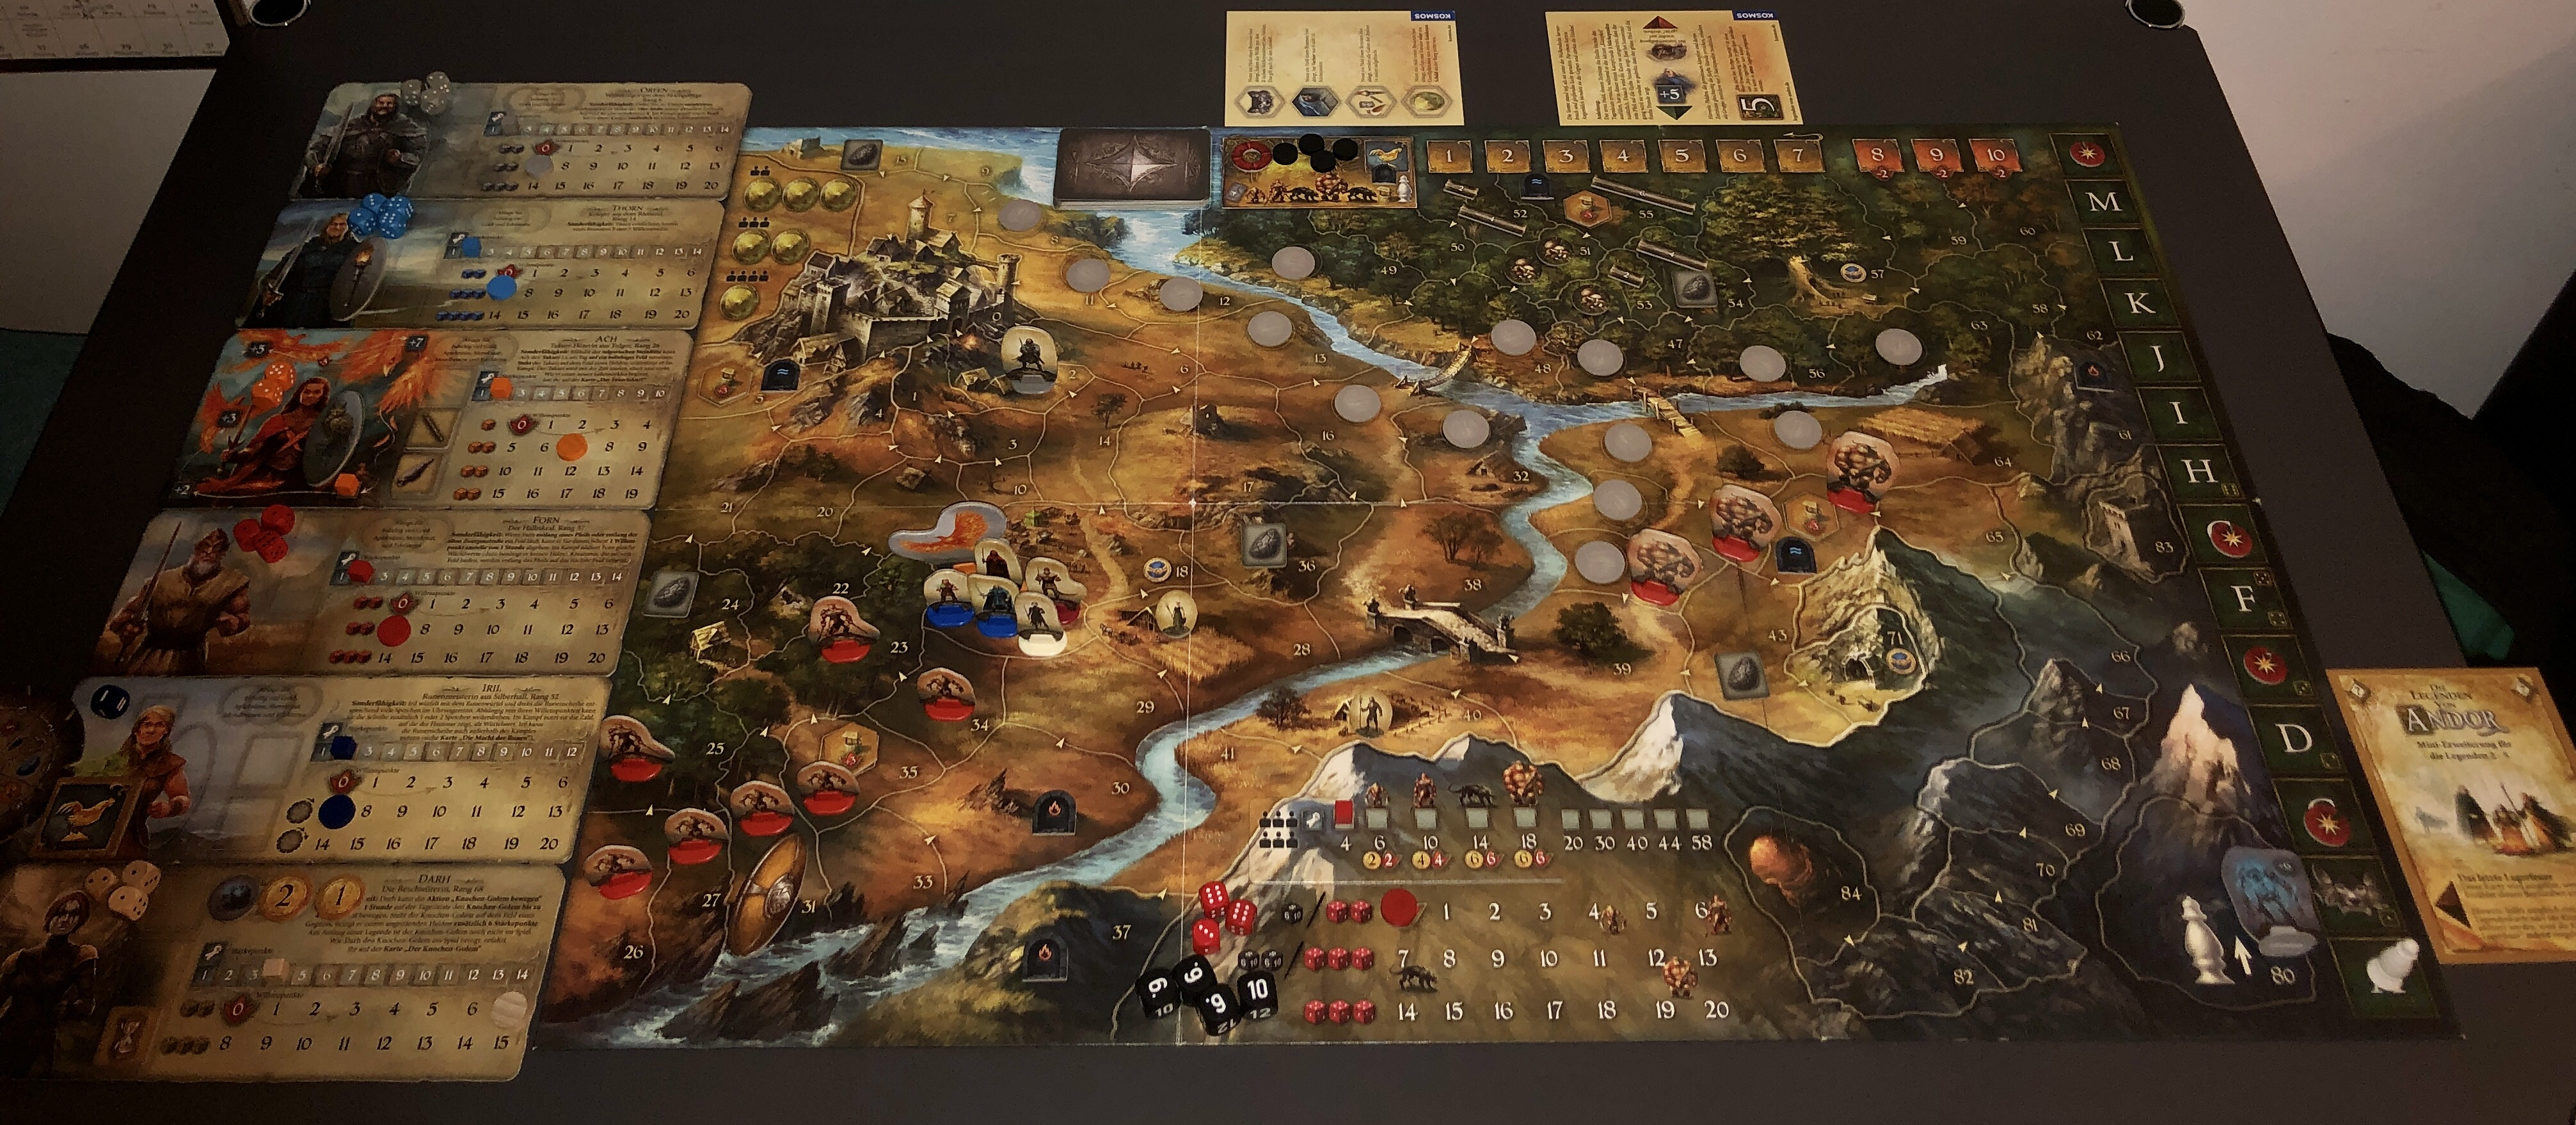
\includegraphics[width=\textwidth]{Das Erbe des Wunderkindes/Bilder/Tag 1 Anfang.jpg}

\textit{Anfang von Tag 1.}\bigskip







Dann geht es los mit Tag 1! :P

Wir zielen zunächst darauf ab, möglichst rasch die Wölfe zu rufen und zu zähmen.



Zuallererst spielt Aćh die andorische Flöte. Der Würfel zeigt eine 4! Die WP aller Helden außer Orfen steigen auf 7 +4 = 11. Dann übergibt Aćh die Flöte an Forn.



Aćh nutzt die Eule 2x, um die 30-Feuertür und die 61-Feuertür zu öffnen. Sie frischt die Eule 2x auf. Aćhs WP sinken auf 11 -3 -3 = 5.

Thorn legt die Fackel von Cavern ab und nimmt die Eule von Aćh an. Er nutzt die Eule 2x, um die 5-Wassertür und die 45-Wassertür zu öffnen. Er frischt die Eule 2x auf. Thorns WP sinken auf 11 -3 -3 = 5.

Wir wissen nun genau, welche Zwergentüren miteinander verbunden sind: 5/61, 45/37 und 55/30.

Thorn gibt die Eule an Forn weiter.



Zug 1: Iril dreht an ihrer Runenscheibe.

In Stunde 1 zeigt der Runenwürfel eine 1. Iril dreht die Runenscheibe um 1 +1 = 2 Speichen auf die 3-WP. Irils WP steigen auf 11 +3 = 14.

Nun befindet sich Iril in ihrer untersten WP-Zeile und kann fortan immer, wenn sie will, ihre Runenscheibe unabhängig vom Runenwürfel jeweils um genau 3 Speichen drehen (1 +2, 2 +1 oder 3 +0).



Zug 2: Darh läuft für 1 Stunde (Zeitstein von 1 auf 2) von 72 auf 18. Darh kauft sich einen Helm. Darhs Gold sinkt auf 3 -2 = 1.



Zug 3: Orfen beendet seinen Tag. Er erhält das Sonnenaufgang-Plättchen.



Zug 4: Thorn beendet seinen Tag.



Zug 5: Aćh nutzt ihre tulgorische Steinflöte. Der Feuertakuri (nennen wir ihn Turr) fliegt von 72 auf 58. Vielleicht taucht Lonas ja dort auf.

Aćh beendet ihren Tag.



Zug 6: Forn läuft für 2 Stunden (Zeitstein von 2 auf 4) von 72 nach 35. Er leert den 35-Brunnen. Forns WP steigen auf 11 +3 = 14.

Darh nutzt das Hadrische Stundenglas, um den Zeitstein von 4 zurück auf 1 zu schieben.



Zug 7: Iril wählt ihre Aktion "Runen befragen". Wann immer sie den 35-Brunnen auffrischt, leert Forn diesen sofort. Einige Quellen dazu:

– Irils Sonder-Aktion kann "Runen befragen" genannt werden.\footnote{Aus der Taverne, "Magische Helden und ein paar allgemeine Fragen": [Giftknödel:] die Aktion "Runen befragen" kostet immer jeweils eine Stunde, genau wie jede einzelne Kampfrunde beim Kämpfen. D.h. zunächst rückt der Zeitstein weiter. Dann werden ggf. WP gezahlt. Und dann folgt die Aktion, also das Drehen der Scheibe.}

– Iril kann auch Brunnen auffrischen, auf deren Feld ein Held steht\footnote{Aus der Taverne, "RF zu den MH Barz, Iril und Aćh in Teil III": [Giftknödel:] Quellen werden nur bei Sonnenaufgang nicht umgedreht, wenn ein Held darauf steht. Die Macht der Runen hingegen vermag das.} (Die Quelle bezieht sich auf Quellen :mrgreen:, aber bei Brunnen sollte das analog funktionieren).

– Zwischen zwei Runenscheiben-Drehungen können freie Handlungsmöglichkeiten ausgeführt werden.\footnote{Aus der Taverne, "Einige Fragen zu den Magischen Helden": [Giftknödel:] Grundsätzlich gilt: Jedes Drehen kostet 1 Stunde. Das Drehen der Scheibe außerhalb des Kampfes ist eine abgeschlossene Aktion. Wenn sie jeweils 1 Stunde zahlt, kann sie diese Aktion auch mehrfach hintereinander tätigen.
Freie Handlungsmöglichkeiten und Standard-Segeln können zwischen den Aktionen ausgeführt werden.} Stellt euch vor, wie nützlich dies erst in Verbindung mit Bragors oder Jarids SF ist. Aber auch Forn kann hübsch davon profitieren. :P

In Stunde 2 dreht Iril die Runenscheibe um 3 Speichen auf den 2-Brunnen. Sie frischt den 35-Brunnen auf. Forn leert den 35-Brunnen. Forns WP steigen auf 14 +3 = 17.

In Stunde 3 dreht Iril die Runenscheibe um 3 Speichen auf den 5-Brunnen. Iril frischt den 35-Brunnen auf. Forn leert den 35-Brunnen. Forns WP steigen auf 17 +3 = 20.



Zug 8: Darh läuft für 1 Stunde (Zeitstein von 3 auf 4) von 18 auf 36. Sie findet einen gelben Runenstein.



Zug 9: Forn läuft für 2 Stunden (Zeitstein von 4 auf 6) von 35 auf 24. Er findet einen grünen Runenstein.

Ich verletze hier die goldene Forn-Regel "Nutze niemals eine Stunde für einen Schritt, für den du auch einen WP bezahlen könntest." Und es gibt nicht einmal einen guten Grund dafür. Ich habe Forns SF hier schlicht und ergreifend übersehen. :oops:



Zug 10: Iril wählt ihre Aktion "Runen befragen".

In Stunde 7 dreht Iril die Runenscheibe um 3 Speichen auf die 3-WP. Irils WP steigen auf 14 +3 = 17.



Zug 11: Darh läuft für 2 Stunden (Zeitstein von 0 auf 2) von 36 auf 72. Sie legt den gelben Runenstein ab.



Zug 12: Forn läuft für 2 Stunden (Zeitstein von 2 auf 4) und 4 WP (Forns WP sinken auf 20 -4 = 16) von 24 über die 5/61-Zwergentüren auf 54. Er findet einen blauen Runenstein.

Forn nutzt die Eule, um Iril den grünen und blauen Runenstein zu schicken.



Zug 13: Iril, nun mit allen drei Runensteinen ausgerüstet, wählt ihre Aktion "Runen befragen".

Wichtig: Iril hat nur zwei kleine Ablagefelder und kann nicht alle drei Runensteine gleichzeitig tragen. Da Iril jedoch zwischen den Runenscheiben-Drehungen freie Handlungsmöglichkeiten (wie das Ablegen und Aufnehmen von Runensteinen) ausführen kann, und da sie bei jeder Drehung auf mindestens einer der drei Runenstein-Speichen gar nicht landen kann, ist es Iril dennoch möglich, immer die passenden Runenstein tragen. Ich werde der Übersicht halber nicht immer extra aufschreiben, welche Runensteine Iril ablegt und aufnimmt.

In Stunde 8 (Irils WP sinken auf 17 -2 = 15) zeigt der Runenwürfel eine 3. Iril dreht die Runenscheibe um 3 +2 = 5 Speichen auf die 4-WP. Irils WP steigen auf 15 +3 = 18.

"4-WP" steht dafür, dass diese Speiche Kampfwert 4 hätte. Die 4-WP-Speiche verschafft auch "nur" +3 WP.

In Stunde 9 (Irils WP sinken auf 18 -2 = 16) zeigt der Runenwürfel eine 2. Iril dreht die Runenscheibe um 2 +0 = 2 Speichen auf den blauen Runenstein. Irils SP steigen auf 2 +1 = 3.

In Stunde 10 (Irils WP sinken auf 16 -2 = 14) dreht Iril die Runenscheibe um 3 Speichen auf den gelben Runenstein. Irils SP steigen auf 3 +1 = 4.



Zug 14: Darh passt (Zeitstein von 4 auf 5).



Zug 15: Forn läuft für 1 WP (Forns WP sinken auf 16 -1 = 15) von 54 auf 47. Das 47-Nebelplättchen versteckte eine Ereigniskarte.

Weiße Ereigniskarte 12 wird ausgelöst. Das Brot aus dem Wachsamen Wald – mit eingebackenen Apfelnüssen – ist allseits bekannt. Ein Brot wird auf 55 eingewürfelt.



Zug 16: Iril wählt ihre Aktion "Runen befragen". Sie nutzt dafür einen noch unbewegten Zeitstein.

In Stunde 1 zeigt der Runenwürfel eine 3. Iril dreht die Runenscheibe um 3 +1 = 4 Speichen auf die 4-WP. Irils WP steigen auf 14 +3 = 17.

In Stunde 2 zeigt der Runenwürfel eine 1. Iril dreht die Runenscheibe um 1 +1 = 2 Speichen auf den blauen Runenstein. Irils SP steigen auf 4 +1 = 5.

In Stunde 3 zeigt der Runenwürfel eine 2. Iril dreht die Runenscheibe um 2 +0 = 2 Speichen auf die 3-WP. Irils WP steigen auf 17 +3 = 20.

In Stunde 4 zeigt der Runenwürfel eine 1. Iril dreht die Runenscheibe um 1 +0 = 1 Speiche auf den gelben Runenstein. Irils SP steigen auf 5 +1 = 6.

In Stunde 5 dreht Iril die Runenscheibe um 3 Speichen auf den grünen Runenstein. Irils SP steigen auf 6 +1 = 7.

In Stunde 6 dreht Iril die Runenscheibe um 3 Speichen auf den blauen Runenstein. Irils SP steigen auf 7 +1 = 8.

In Stunde 7 dreht Iril die Runenscheibe um 3 Speichen auf den gelben Runenstein. Irils SP steigen auf 8 +1 = 9.

In Stunde 8 (Irils WP sinken auf 20 -2 = 18) dreht Iril die Runenscheibe um 3 Speichen auf den grünen Runenstein. Irils SP steigen auf 9 +1 = 10.

In Stunde 9 (Irils WP sinken auf 18 -2 = 16) dreht Iril die Runenscheibe um 3 Speichen auf den blauen Runenstein. Irils SP steigen auf 10 +1 = 11.

In Stunde 10 (Irils WP sinken auf 16 -2 = 14) dreht Iril die Runenscheibe um 3 Speichen auf den gelben Runenstein. Irils SP steigen auf 11 +1 = 12.

Volle Stärkeleiste für Iril! :D



Zug 17: Darh läuft für 1 Stunde (Zeitstein von 5 auf 6) von 72 auf 23. Dieser Skral soll noch heute fallen. Sie nimmt dabei die Fackel von Cavern und einen von Irils Runensteinen von 72 mit, legt diese aber direkt wieder auf 23 ab.



Zug 18: Forn läuft für 1 WP (seine WP sinken auf 15 -1 = 14) von 47 auf 46. Das 46-Nebelplättchen versteckte Reka. Reka wird auf 46 aufgestellt. Forn erhält einen Trank der Hexe.



Zug 19: Iril läuft für 1 Stunde (Zeitstein von 6 auf 7) von 72 auf 23. Sie nimmt die schlafende Eule und zwei Runensteine mit.



Zug 20: Darh lädt Iril zum gemeinsamen Kämpfen gegen den 23-Skral ein.

In Kampfrunde 1 (Zeitsteine von 0 auf 1 und von 7 auf 8, Darhs WP sinken auf 11 -2 = 9) zeigt der Runenwürfel eine 1. Iril dreht die Runenscheibe um 1 +0 = 1 Speiche auf das 5-Auge. Die Helden haben einen Kampfwert von 4 SP (Darh) +12 SP (Iril) +4 (Darhs Würfel) +5 (Irils Speiche) = 25.

Der 23-Skral hat einen Kampfwert von 10 SP +4 = 14.

Der 23-Skral ist besiegt.

Belohnung: Darhs Gold steigt auf 1 +4 = 5.

Darh beschwört ihren Knochen-Golem. Er wird samt Skral auf Feld 41 eingewürfelt (oh nein, das bedroht Casimirs Bruder auf 41). Das Golem-Symbol kommt auf E.

Der Erzähler läuft auf B.

Die Wölfe (nennen wir sie Lonas, Rutan und Merla) werden eingewürfelt. Lonas erscheint auf 64, Merla auf 33 und Rutan auf 43. Das Wolfssymbol wird auf Stunde 4 gewürfelt.

Das letzte Lagerfeuer wird ausgelöst. Die Helden verteilen ihre SP und WP neu:



Orfen: 2 SP, 7 WP –> 1 SP, 1 WP

Thorn: 2 SP, 5 WP –> 3 SP, 4 WP

Aćh: 2 SP, 5 WP –> 4 SP, 8 WP

Forn: 2 SP, 14 WP –> 14 SP, 20 WP

Iril: 12 SP, 14 WP –> 1 SP, 15 WP

Darh: 4 SP, 9 WP –> 1 SP, 6 WP



Zug 21: Forn läuft für 1 Stunde (Zeitstein von 1 auf 2) von 64 auf 45.

Forn opfert den 45-Brunnen den Wunschbrunnen. Er wünscht sich schwächere Wölfe.



Zug 22: Iril wählt ihre Aktion "Runen befragen".

In Stunde 3 zeigt der Runenwürfel eine 1. Iril dreht die Runenscheibe um 1 +2 = 3 Speichen auf die 4-WP. Ihre WP steigen auf 15 +3 = 18.

In Stunde 4 (das Wolfssymbol wird ausgelöst; Merla läuft von 33 auf 30, Rutan von 43 auf 39 und Lonas von 64 auf 45) zeigt der Runenwürfel eine 2. Iril dreht die Runenscheibe um 2 +0 = 2 Speichen auf den blauen Runenstein. Ihre SP steigen auf 1 +1 = 2.



Zug 23: Darh wählt ihre Aktion "Knochen-Golem bewegen". Der Knochen-Golem läuft für 1 Stunde (Zeitstein von 8 auf 9, Darhs WP sinken auf 6 -2 = 4) von 41 auf 45.



Zug 24: Forn bekämpft Lonas auf 45.

In Kampfrunde 1 (Zeitstein von 4 auf 5, das Licht der fünften Stunde wird ausgelöst) hat Forn einen Kampfwert von 14 SP +6 (Knochen-Golem) +5 (Licht der fünften Stunde) + 5 (Würfel) = 30. Der gewünschte Kampfwert von 2x14 = 28 ist somit erreicht.

Die Wölfe sind gezähmt und jeder von ihnen ist glorreiche 14 SP wert! Forn ist der Wolfsfreund. Diese Verbindung soll nicht vergessen gehen, denn beinahe ein Jahrzehnt später wird Forn der erste von Lonas aufgespürte Dunkle Held werden – wobei Forn sich dann wieder vor Lonas fürchten wird.



Kurze Tangente: Theoretisch wäre auch ohne Wunschbrunnen eine Wolfsstärke von 14 (d.h. ein Zähmwert 4x14 = 56) möglich, aber nur mithilfe von unglaublichem Glück wie 14-SP-Thorn +7 (Turr) +6 (Knochen-Golem) +5 (Licht der fünften Stunde) +24 (6er-Pasch mit 4 Würfeln) = 56 oder aber mithilfe von Verbrauchsgegenständen wie 14-SP-Eara +7 (Turr) +6 (Knochen-Golem) +5 (Licht der fünften Stunde) +6 (minimum Wassergeist-Würfel) +6 (Trank der Hexe) +4 (Heilkraut) +4 (Heilkraut) +4 (Kampfaxt) = 56.



Zug 25: Iril wählt ihre Aktion "Runen befragen".

In Stunde 10 (Irils WP sinken auf 18 -2 = 16) dreht Iril die Runenscheibe um 3 Speichen auf den gelben Runenstein. Irils SP steigen auf 2 +1 = 3.



Zug 26: Darh beendet ihren Tag.



Zug 27: Forn läuft für 3 Stunden (Zeitstein von 5 auf 8, Forns WP sinken auf 20 -2 = 18) und 8 WP (Forns WP sinken auf 18 -8 = 10) von 45 über 40, 28 und 0 auf 5. Er nimmt im Vorbeigehen die beiden Bauern von 40 und 28 auf 0 mit. Zwei goldene Schilde mehr für die Rietburg!

Forn leert den 5-Brunnen. Forns WP steigen auf 10 +3 = 13.



Zug 28: Iril wählt ihre Aktion "Runen befragen".

In Stunde 9 (Irils WP sinken auf 16 -2 = 14) dreht Iril die Runenscheibe um 3 Speichen auf den grünen Runenstein. Irils SP steigen auf 3 +1 = 4.



Zug 29: Forn läuft für 1 Stunde (Zeitstein von 9 auf 10, Forns WP sinken auf 13 -2 = 11) über die Zwergentür von 5 auf 61. Er könnte zwar noch weiterrennen, wartet aber wohlweislich hier auf das Einwürfeln der C-Heilkräuter.



Zug 30: Iril beendet ihren Tag.



Zug 31: Forn beendet seinen Tag.\bigskip






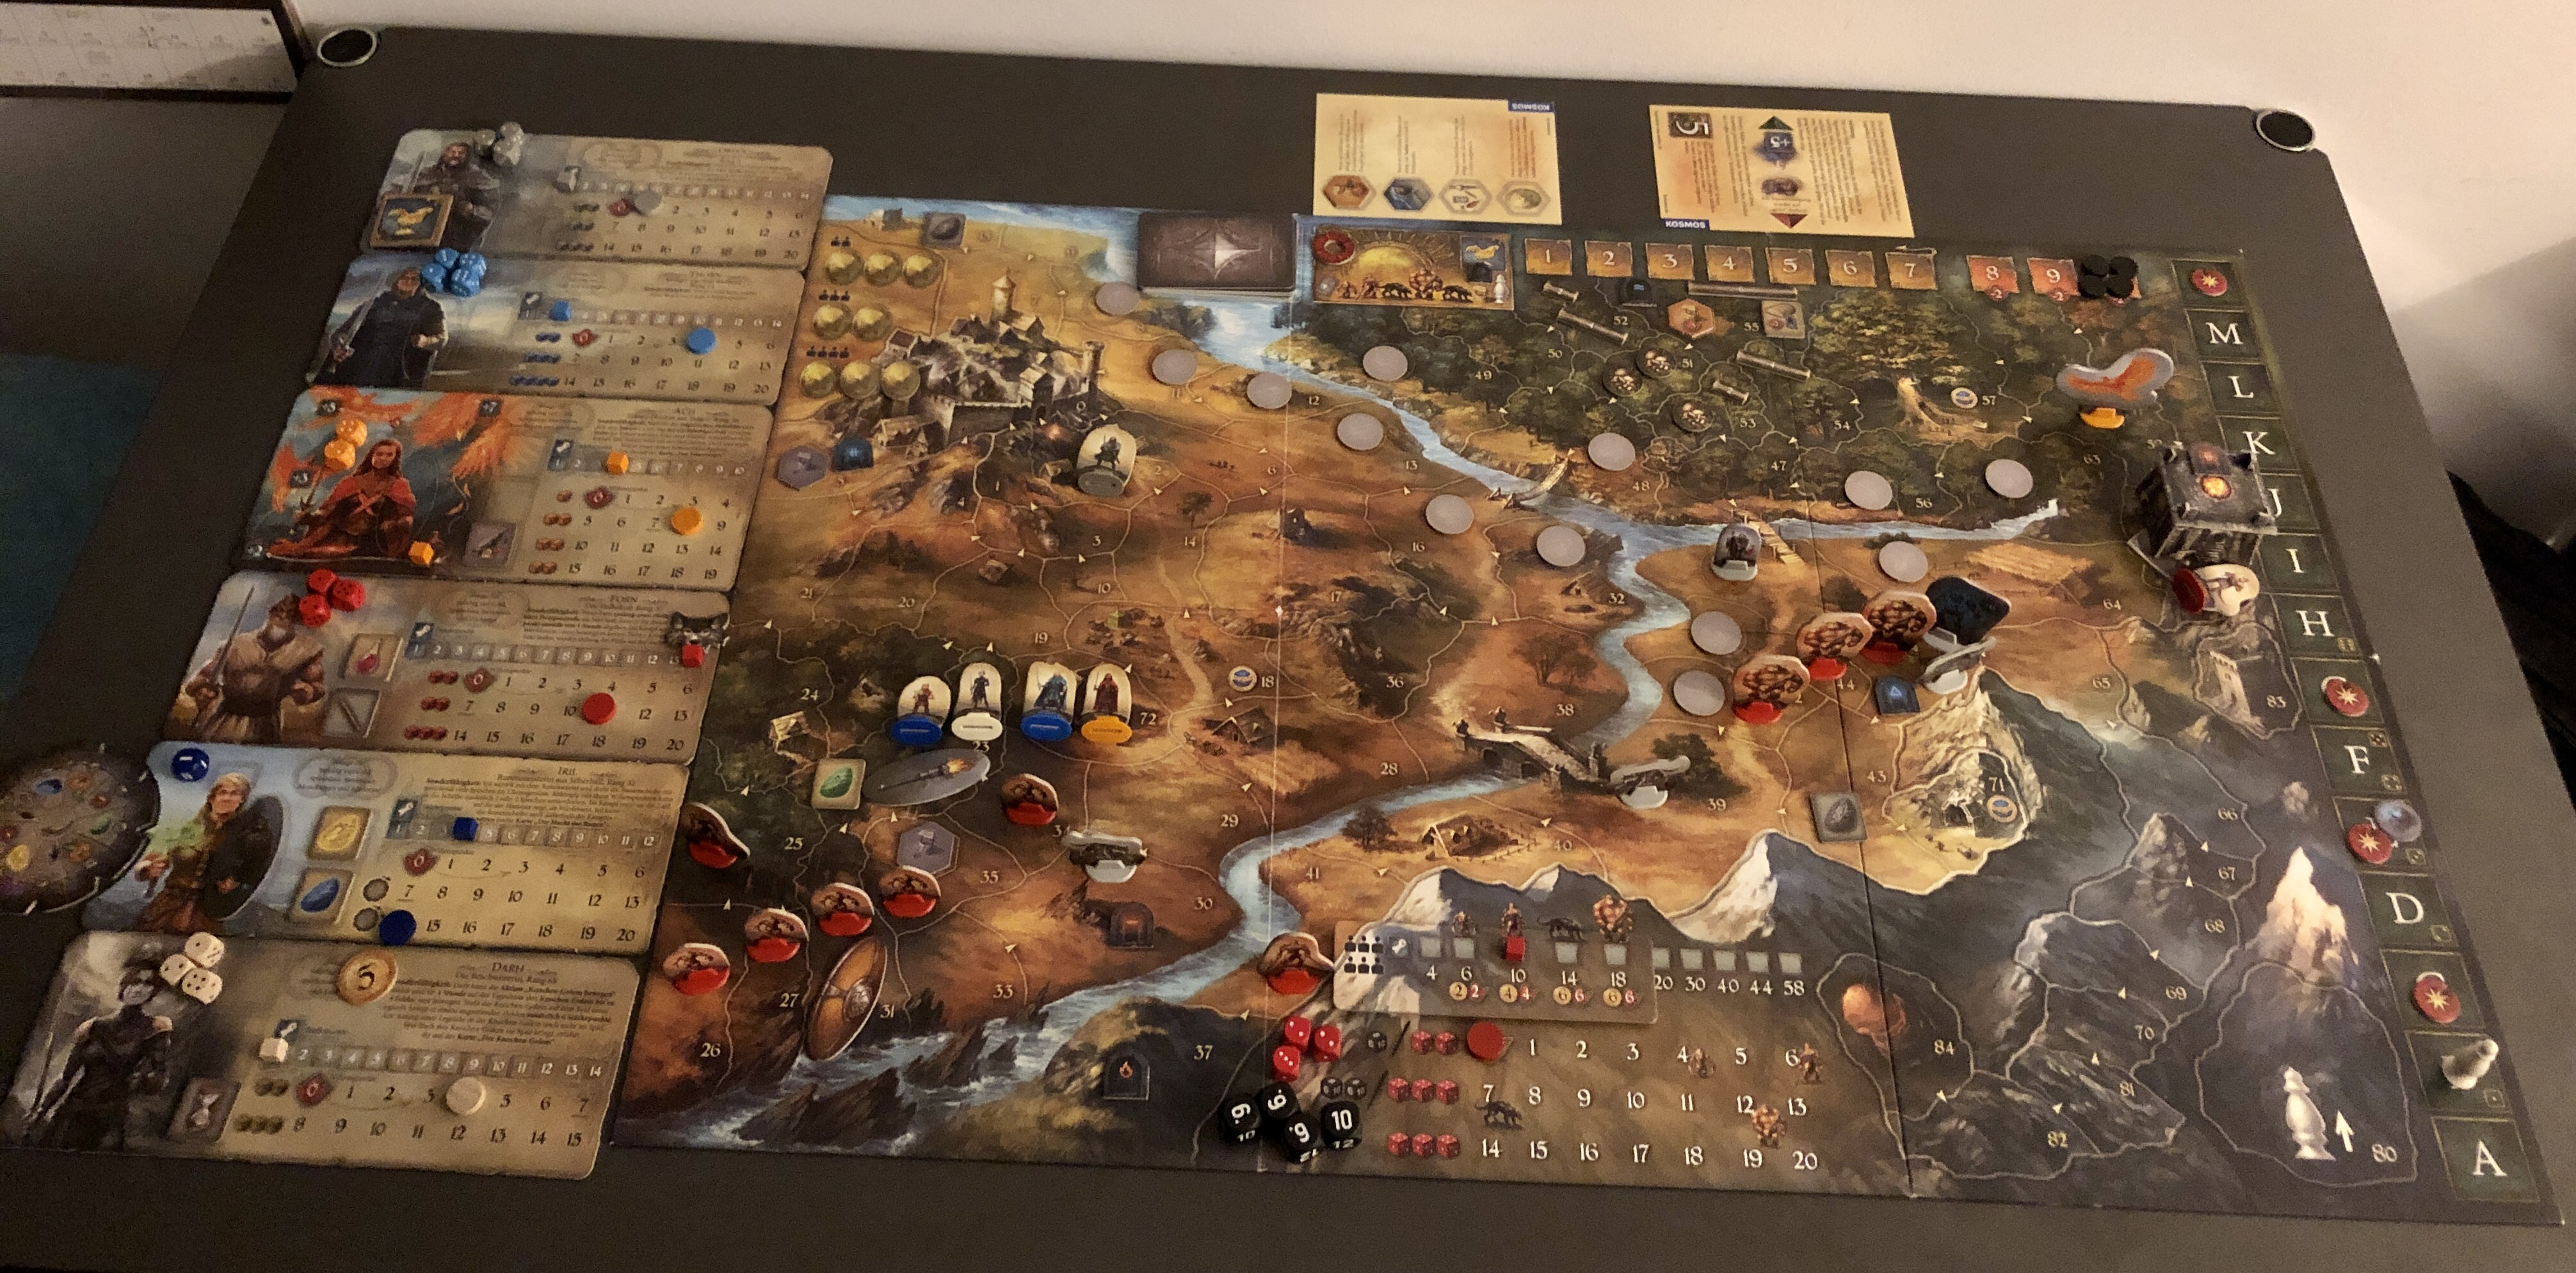
\includegraphics[width=\textwidth]{Das Erbe des Wunderkindes/Bilder/Tag 1 Ende.jpg}



\textit{Ende von Tag 1.}

\textit{Korrektur: Der Takuri-Marker sollte bereits auf +2 liegen.}


\newpage
\section{Tag 2}


Sonnenaufgang:

Weiße Ereigniskarte 14 wird ausgelöst. Im Wachsamen Wald liegt eine Waffe aus den Trollkriegen versteckt. Auf 54 wird ein Messer eingewürfelt.

Die Kreaturen laufen, die Brunnen werden aufgefrischt, die Zwergentüren werden geschlossen und der Erzähler läuft auf C.

Legendenkarte C wird ausgelöst. Zwei Heilkräuter werden eingewürfelt auf 25 und 16. Ein Skral erscheint zufällig auf 36.

Die Bedrohung ist ... Trommelwirbel ... der Belagerungsturm! Er erscheint auf 84 und wird jeden Sonnenaufgang so viele Felder bewegt, wie Kreaturen auf Spielfeldern stehen.\bigskip


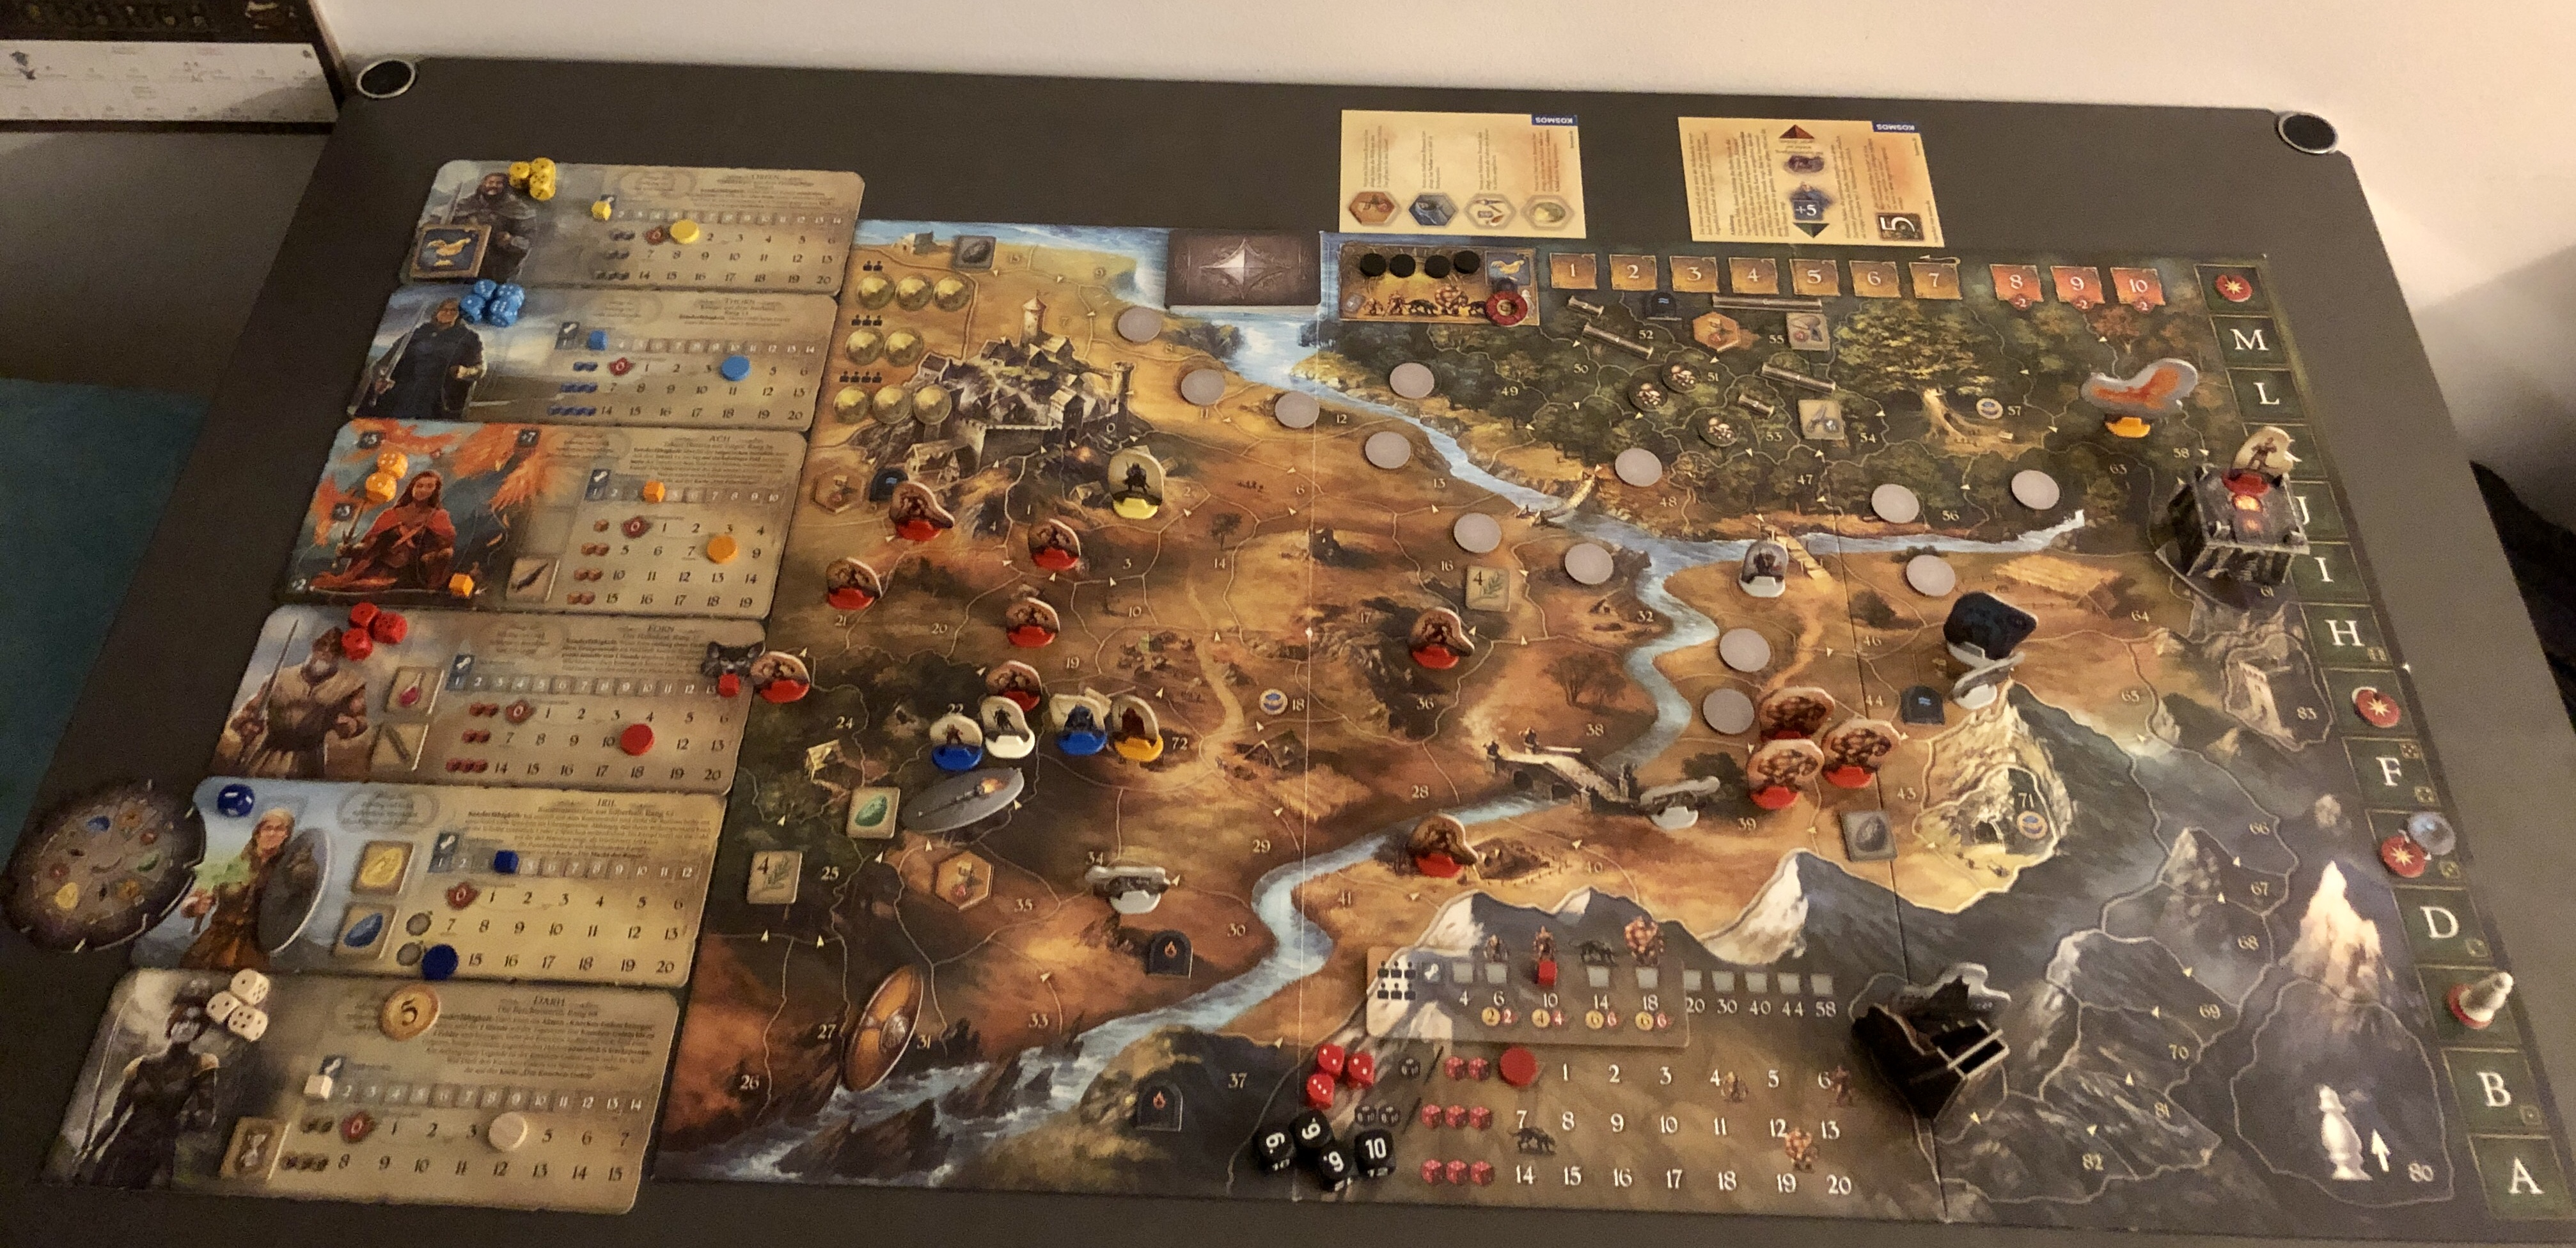
\includegraphics[width=\textwidth]{Das Erbe des Wunderkindes/Bilder/Tag 2 Anfang.jpg}


\textit{Anfang von Tag 2.}

\textit{Korrekturen: Der Takuri-Marker sollte bereits auf +3 liegen. Die beiden 4er-Heilkräuter sollten verdeckt sein. Und was macht denn der Dunkle Tempel da?}\bigskip




Zug 1: Orfen beendet seinen Tag. Er behält das Sonnenaufgang-Plättchen gleich.



Zug 2: Thorn beendet seinen Tag.



Zug 3: Aćh nutzt ihre tulgorische Steinflöte. Turr fliegt von 58 auf 16, wo am nächsten Tag der 36-Skral stehen wird.

Aćh beendet ihren Tag.



Zug 4: Forn läuft für 3 WP (Forns WP sinken auf 11 -3 = 8) von 61 auf 54. Er nimmt den 4er-Holzstamm und das Messer auf.



Zug 5: Iril wählt ihre Aktion "Runen befragen".

In Stunde 1 zeigt der Runenwürfel eine 3. Iril dreht die Runenscheibe um 3 +2 = 5 Speichen auf die 3-WP. Irils WP steigen auf 14 +3 = 17.

In Stunde 2 zeigt der Runenwürfel eine 2. Iril dreht die Runenscheibe um 2 +2 = 4 Speichen auf den grünen Runenstein. Irils SP steigen auf 4 +1 = 5.

In Stunde 3 zeigt der Runenwürfel eine 1. Iril dreht die Runenscheibe um 1 +0 = 2 Speichen auf die 4-WP. Irils WP steigen auf 17 +3 = 20.

In Stunde 4 zeigt der Runenwürfel eine 1. Iril dreht die Runenscheibe um 1 +1 = 2 Speichen auf den blauen Runenstein. Irils SP steigen auf 5 +1 = 6.

In Stunde 5 dreht Iril die Runenscheibe um 3 Speichen auf den gelben Runenstein. Irils SP steigen auf 6 +1 = 7.

In Stunde 6 dreht Iril die Runenscheibe um 3 Speichen auf den grünen Runenstein. Irils SP steigen auf 7 +1 = 8.

In Stunde 7 dreht Iril die Runenscheibe um 3 Speichen auf den blauen Runenstein. Irils SP steigen auf 8 +1 = 9.

In Stunde 8 (Irils WP sinken auf 20 -2 = 18) dreht Iril die Runenscheibe um 3 Speichen auf den gelben Runenstein. Irils SP steigen auf 9 +1 = 10.

In Stunde 9 (Irils WP sinken auf 18 -2 = 16) dreht Iril die Runenscheibe um 3 Speichen auf den gelben Runenstein. Irils SP steigen auf 10 +1 = 11.

In Stunde 10 (Irils WP sinken auf 16 -2 = 14) dreht Iril die Runenscheibe um 3 Speichen auf den gelben Runenstein. Irils SP steigen auf 11 +1 = 12.

Volle Stärkeleiste für Iril, schon zum zweiten Mal! :P



Zug 6: Darh läuft für 1 Stunde (Zeitstein von 0 auf 1) von 23 auf 31. Sie findet den Bruderschild.

Darh nutzt die erste Seite des Bruderschilds, um ihren 1 SP mit Irils 12 SP zu tauschen.



Zug 7: Forn läuft für 1 Stunde (Zeitstein von 1 auf 2) von 54 auf 53. Er findet einen 2er-Holzstamm und einen 2er-Waldpilz. Forns Gold steigt quasi auf 0 +2 = 2.



Zug 8: Iril wählt ihre Aktion "Runen befragen".

In Stunde 1 zeigt der Runenwürfel eine 2. Iril dreht die Runenscheibe um 2 +2 = 4 Speichen auf die 4-WP. Irils WP steigen auf 14 +3 = 17.

In Stunde 2 zeigt der Runenwürfel eine 3. Iril dreht die Runenscheibe um 3 +1 = 4 Speichen auf die 3-WP. Irils WP steigen auf 17 +3 = 20.

In Stunde 3 zeigt der Runenwürfel eine 1. Iril dreht die Runenscheibe um 2 +2 = 4 Speichen auf den grünen Runenstein. Irils SP steigen auf 1 +1 = 2.

In Stunde 4 dreht Iril die Runenscheibe um 3 Speichen auf den blauen Runenstein. Irils SP steigen auf 2 +1 = 3.

In Stunde 5 dreht Iril die Runenscheibe um 3 Speichen auf den gelben Runenstein. Irils SP steigen auf 3 +1 = 4.

In Stunde 6 dreht Iril die Runenscheibe um 3 Speichen auf den grünen Runenstein. Irils SP steigen auf 4 +1 = 5.

In Stunde 7 dreht Iril die Runenscheibe um 3 Speichen auf den blauen Runenstein. Irils SP steigen auf 5 +1 = 6.

In Stunde 8 (Irils WP sinken auf 20 -2 = 18) dreht Iril die Runenscheibe um 3 Speichen auf den gelben Runenstein. Irils SP steigen auf 6 +1 = 7.

In Stunde 9 (Irils WP sinken auf 18 -2 = 16) dreht Iril die Runenscheibe um 3 Speichen auf den gelben Runenstein. Irils SP steigen auf 7 +1 = 8.

In Stunde 10 (Irils WP sinken auf 16 -2 = 14) dreht Iril die Runenscheibe um 3 Speichen auf den gelben Runenstein. Irils SP steigen auf 8 +1 = 9.



Zug 9: Darh läuft für 1 Stunde (Zeitstein von 2 auf 3) von 31 auf 25. Sie findet ein 4-Heilkraut.

Darh nutzt das Hadrische Stundenglas, um den den Zeitstein von 3 zurück auf 0 zu schieben.



Zug 10: Forn läuft für 1 Stunde (Zeitstein von 0 auf 1) von 53 auf 55. Er leert den 55-Brunnen. Forns WP steigen auf 8 +3 = 11.

Forn nimmt den 6er-Holzstamm auf.

Iril schickt die Eule (ohne Inhalt) an Forn

Forn frischt die Eule für 3 WP auf. Forns WP sinken auf 11 -3 = 8.

Forn schickt den Trank der Hexe samt Eule zurück an Iril. Iril legt die schlafende Eule und den Trank der Hexe auf 23 ab.

Forn nimmt das Brot auf 55 auf und schon sind seine kleinen Ablagefelder wieder gefüllt.



Zug 11: Iril wählt ihre Aktion "Runen befragen".

In Stunde 1 zeigt der Runenwürfel eine 3. Iril dreht die Runenscheibe um 3 +1 = 4 Speichen auf die 4-WP. Irils WP steigen auf 14 +3 = 17.

In Stunde 2 zeigt der Runenwürfel eine 1. Iril dreht die Runenscheibe um 1 +1 = 2 Speichen auf den blauen Runenstein. Irils SP steigen auf 9 +1 = 10.

In Stunde 3 zeigt der Runenwürfel eine 3. Iril dreht die Runenscheibe um 3 +0 = 3 Speichen auf den gelben Runenstein. Irils SP steigen auf 10 +1 = 11.

In Stunde 4 zeigt der Runenwürfel eine 2. Iril dreht die Runenscheibe um 2 +2 = 4 Speichen auf die 4-WP. Irils WP steigen auf 17 +3 = 20.

In Stunde 5 zeigt der Runenwürfel eine 2. Iril dreht die Runenscheibe um 2 +0 = 2 Speichen auf den blauen Runenstein. Irils SP steigen auf 11 +1 = 12.

Volle Stärkeleiste für Iril, zum dritten Mal! :D



Zug 12: Darh läuft für 1 Stunde (Zeitstein von 1 auf 2) von 25 auf 23.

Darh übergibt Iril den Bruderschild und nimmt die schlafende Eule auf. Iril nutzt die zweite Seite des Bruderschilds, um ihre 12 SP mit Orfens 1 SP zu tauschen.



Zug 13: Forn läuft für 1 WP (Forns WP sinken auf 8 -1 = 7) von 55 auf 51. Er findet 2 1er-Waldpilze. Forns Gold steigt quasi auf 2 +2 = 4.



Zug 14: Iril wählt ihre Aktion "Runen befragen".

In Stunde 6 dreht Iril die Runenscheibe um 3 Speichen auf den gelben Runenstein. Irils SP steigen auf 1 +1 = 2.

In Stunde 7 dreht Iril die Runenscheibe um 3 Speichen auf den grünen Runenstein. Irils SP steigen auf 2 +1 = 3.

In Stunde 8 (Irils WP sinken auf 20 -2 = 18) dreht Iril die Runenscheibe um 3 Speichen auf den blauen Runenstein. Irils SP steigen auf 3 +1 = 4.

In Stunde 9 (Irils WP sinken auf 18 -2 = 16) dreht Iril die Runenscheibe um 3 Speichen auf den gelben Runenstein. Irils SP steigen auf 4 +1 = 5.

In Stunde 10 (Irils WP sinken auf 16 -2 = 14) dreht Iril die Runenscheibe um 3 Speichen auf den grünen Runenstein. Irils SP steigen auf 5 +1 = 6.



Zug 15: Darh beendet ihren Tag.



Zug 16: Forn läuft für 1 WP (Forns WP sinken auf 7 -1 = 6) von 51 auf 48. Das 48-Nebelplättchen versteckte eine Ereigniskarte.

Weiße Ereigniskarte 16 wird ausgelöst. Im hohen Rietgras verstecken sich Waffen aus der großen Schlacht um die Rietburg (im Lied des Königs?). Bei Betrams Hof (24) wird ein Messer eingewürfelt.



Zug 17: Iril wählt ihre Aktion "Runen befragen".

In Stunde 3 zeigt der Runenwürfel eine 1. Iril dreht die Runenscheibe um 1 +0 = 1 Speiche auf die 4-WP. Irils WP steigen auf 14 +3 = 17.

In Stunde 4 zeigt der Runenwürfel eine 3. Iril dreht die Runenscheibe um 3 +1 = 4 Speichen auf die 3-WP. Irils WP steigen auf 17 +3 = 20.

In Stunde 5 zeigt der Runenwürfel eine 1. Iril dreht die Runenscheibe um 1 +0 = 1 Speiche auf den gelben Runenstein. Irils SP steigen auf 6 +1 = 7.

In Stunde 6 dreht Iril die Runenscheibe um 3 Speichen auf den grünen Runenstein. Irils SP steigen auf 7 +1 = 8.

In Stunde 7 dreht Iril die Runenscheibe um 3 Speichen auf den blauen Runenstein. Irils SP steigen auf 8 +1 = 9.

In Stunde 8 (Irils WP sinken auf 20 -2 = 18) dreht Iril die Runenscheibe um 3 Speichen auf den gelben Runenstein. Irils SP steigen auf 9 +1 = 10.

In Stunde 9 (Irils WP sinken auf 18 -2 = 16) dreht Iril die Runenscheibe um 3 Speichen auf den gelben Runenstein. Irils SP steigen auf 10 +1 = 11.

In Stunde 10 (Irils WP sinken auf 16 -2 = 14) dreht Iril die Runenscheibe um 3 Speichen auf den gelben Runenstein. Irils SP steigen auf 11 +1 = 12.

Volle Stärkeleiste für Iril, zum vierten Mal! :P

Iril legt alle drei Runensteine auf 23 ab.



Zug 18: Forn läuft für 4 WP (Forns WP sinken auf 6 -4 = 2) von 48 auf 0.

Forn lädt alle Holzstämme ab.

Die Fürstenaufgabe ist erfüllt! :D

Forn nutzt die andorische Flöte. Der Würfel zeigt eine 2! Forns WP steigen auf 2 +2 = 4. Da Orfen auf 2 angrenzend zu 0 schläft, steigen auch Orfens WP auf 1 +2 = 3.



Zug 19: Iril beendet ihren Tag.



Zug 20: Forn beendet seinen Tag.\bigskip





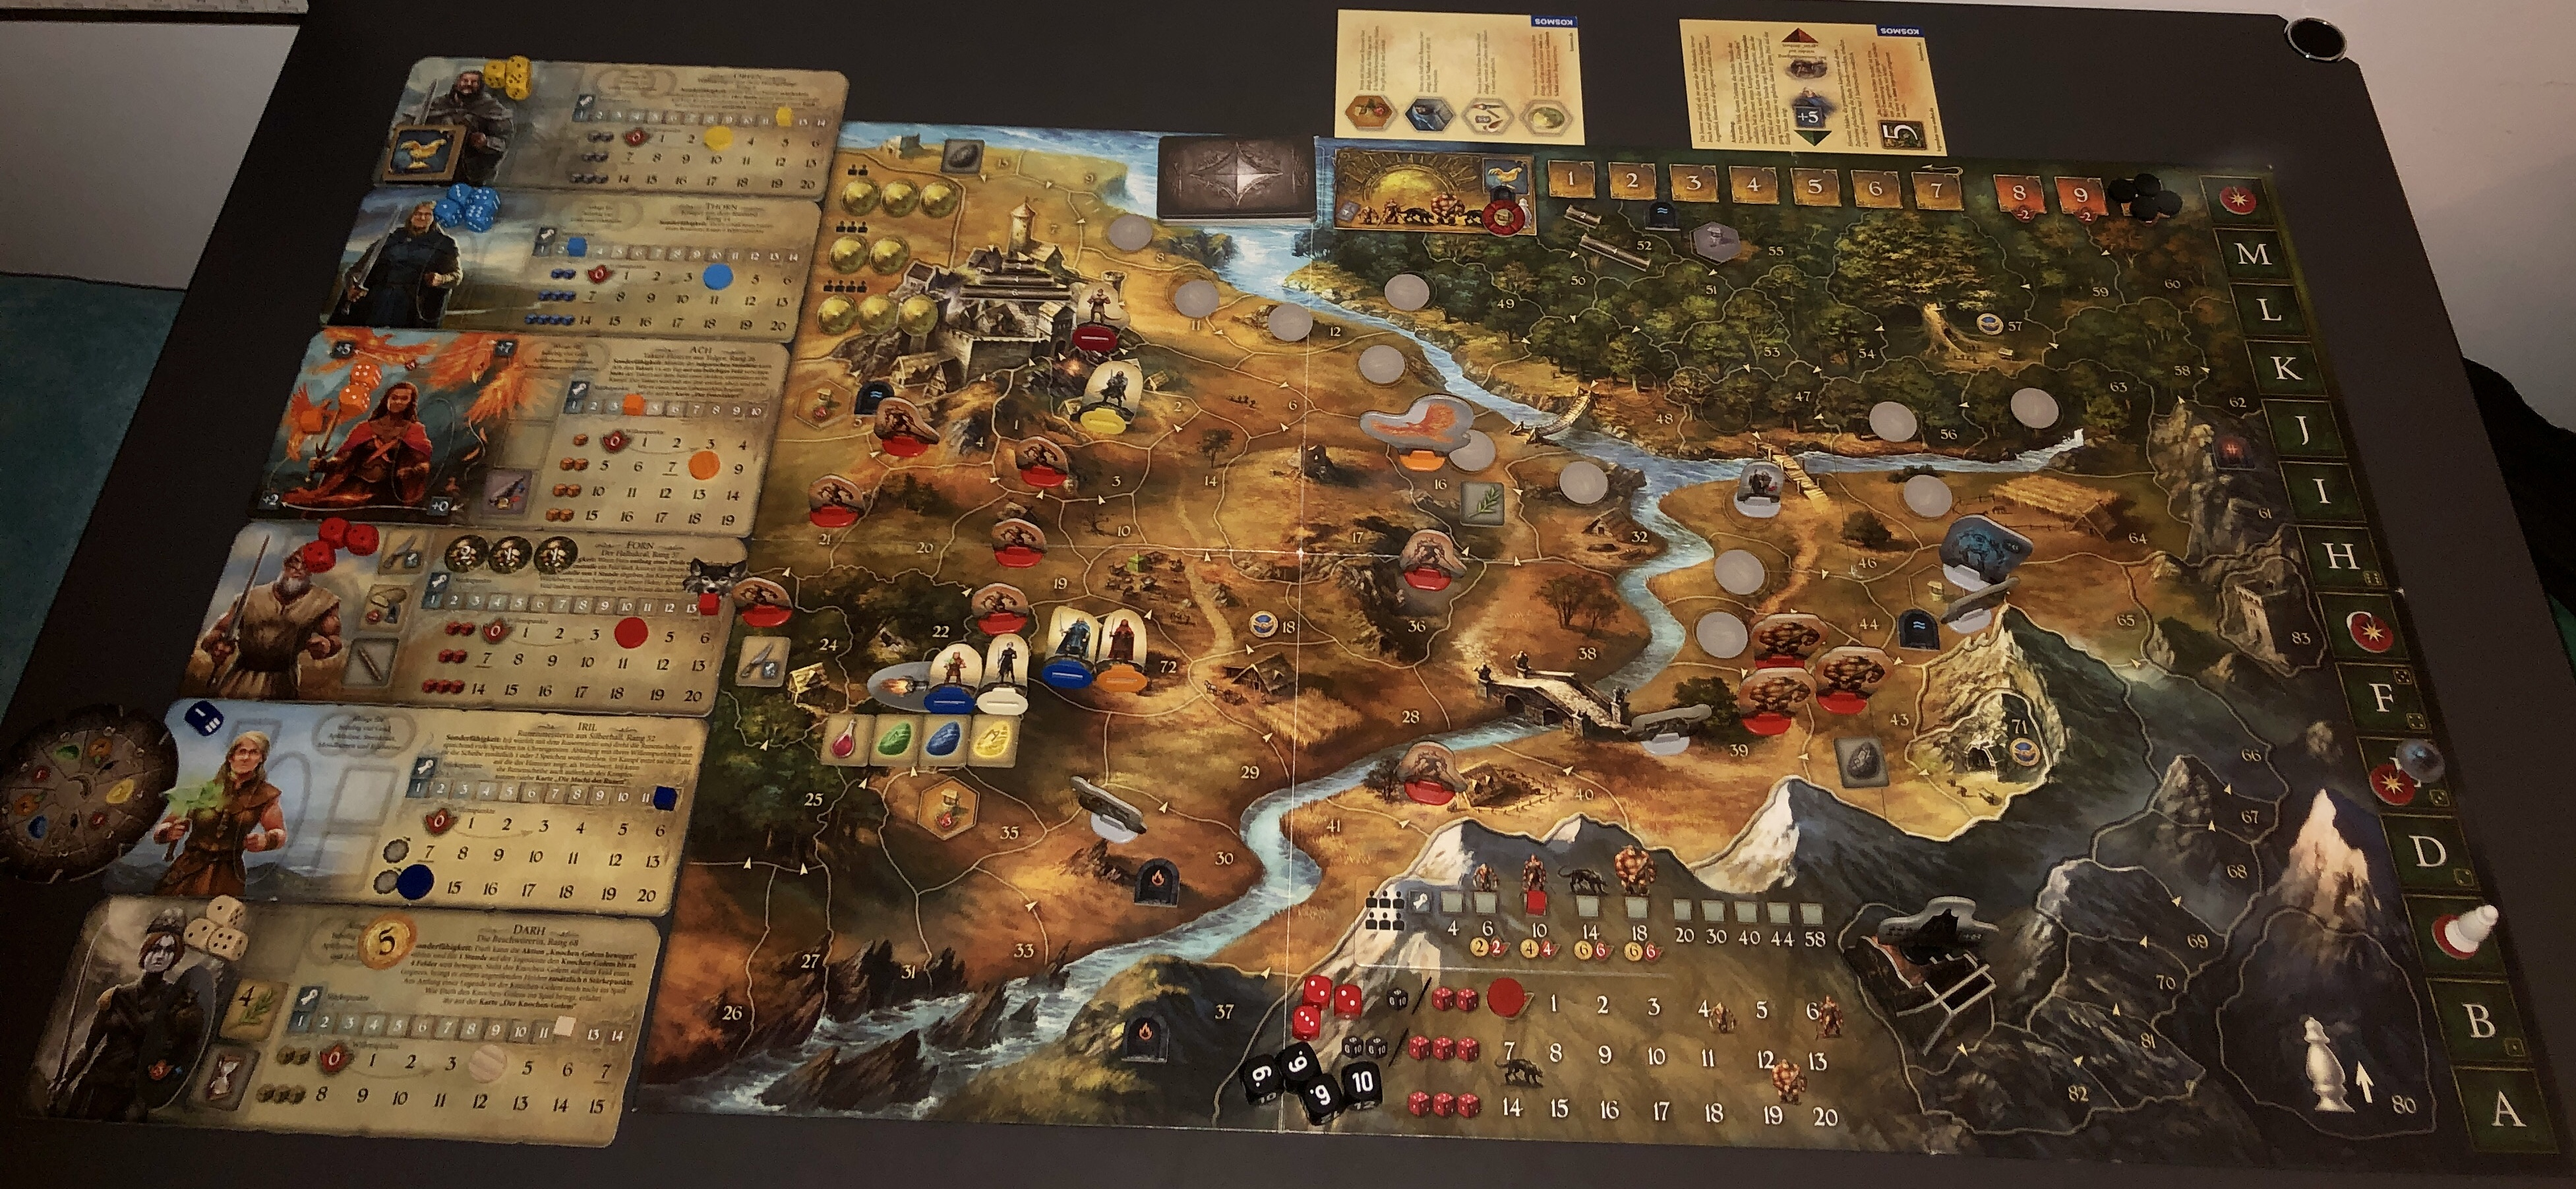
\includegraphics[width=\textwidth]{Das Erbe des Wunderkindes/Bilder/Tag 2 Ende.jpg}

\textit{Ende von Tag 2.}

\newpage
\section{Tag 3}


Sonnenaufgang:

Weiße Ereigniskarte 6 wird ausgelöst. Der gute Wille und die Kraft des andorischen Volkes begleitete die Helden – der gute Wille begleitet Aćh und die Kraft begleitet Orfen. Aćhs WP steigen auf 8 +2 = 10. Orfens SP steigen auf 12 +1 = 13.

Die Kreaturen laufen, davon ein Gor und ein Skral direkt in die Burg.

Der 55-Brunnen werden aufgefrischt. Die 61-Zwergentür wird geschlossen. Es sind aktuell noch 9 Kreaturen im Spiel. Der Belagerungsturm läuft 9 Schritte von 84 auf 45.

Der Erzähler läuft auf D.\bigskip


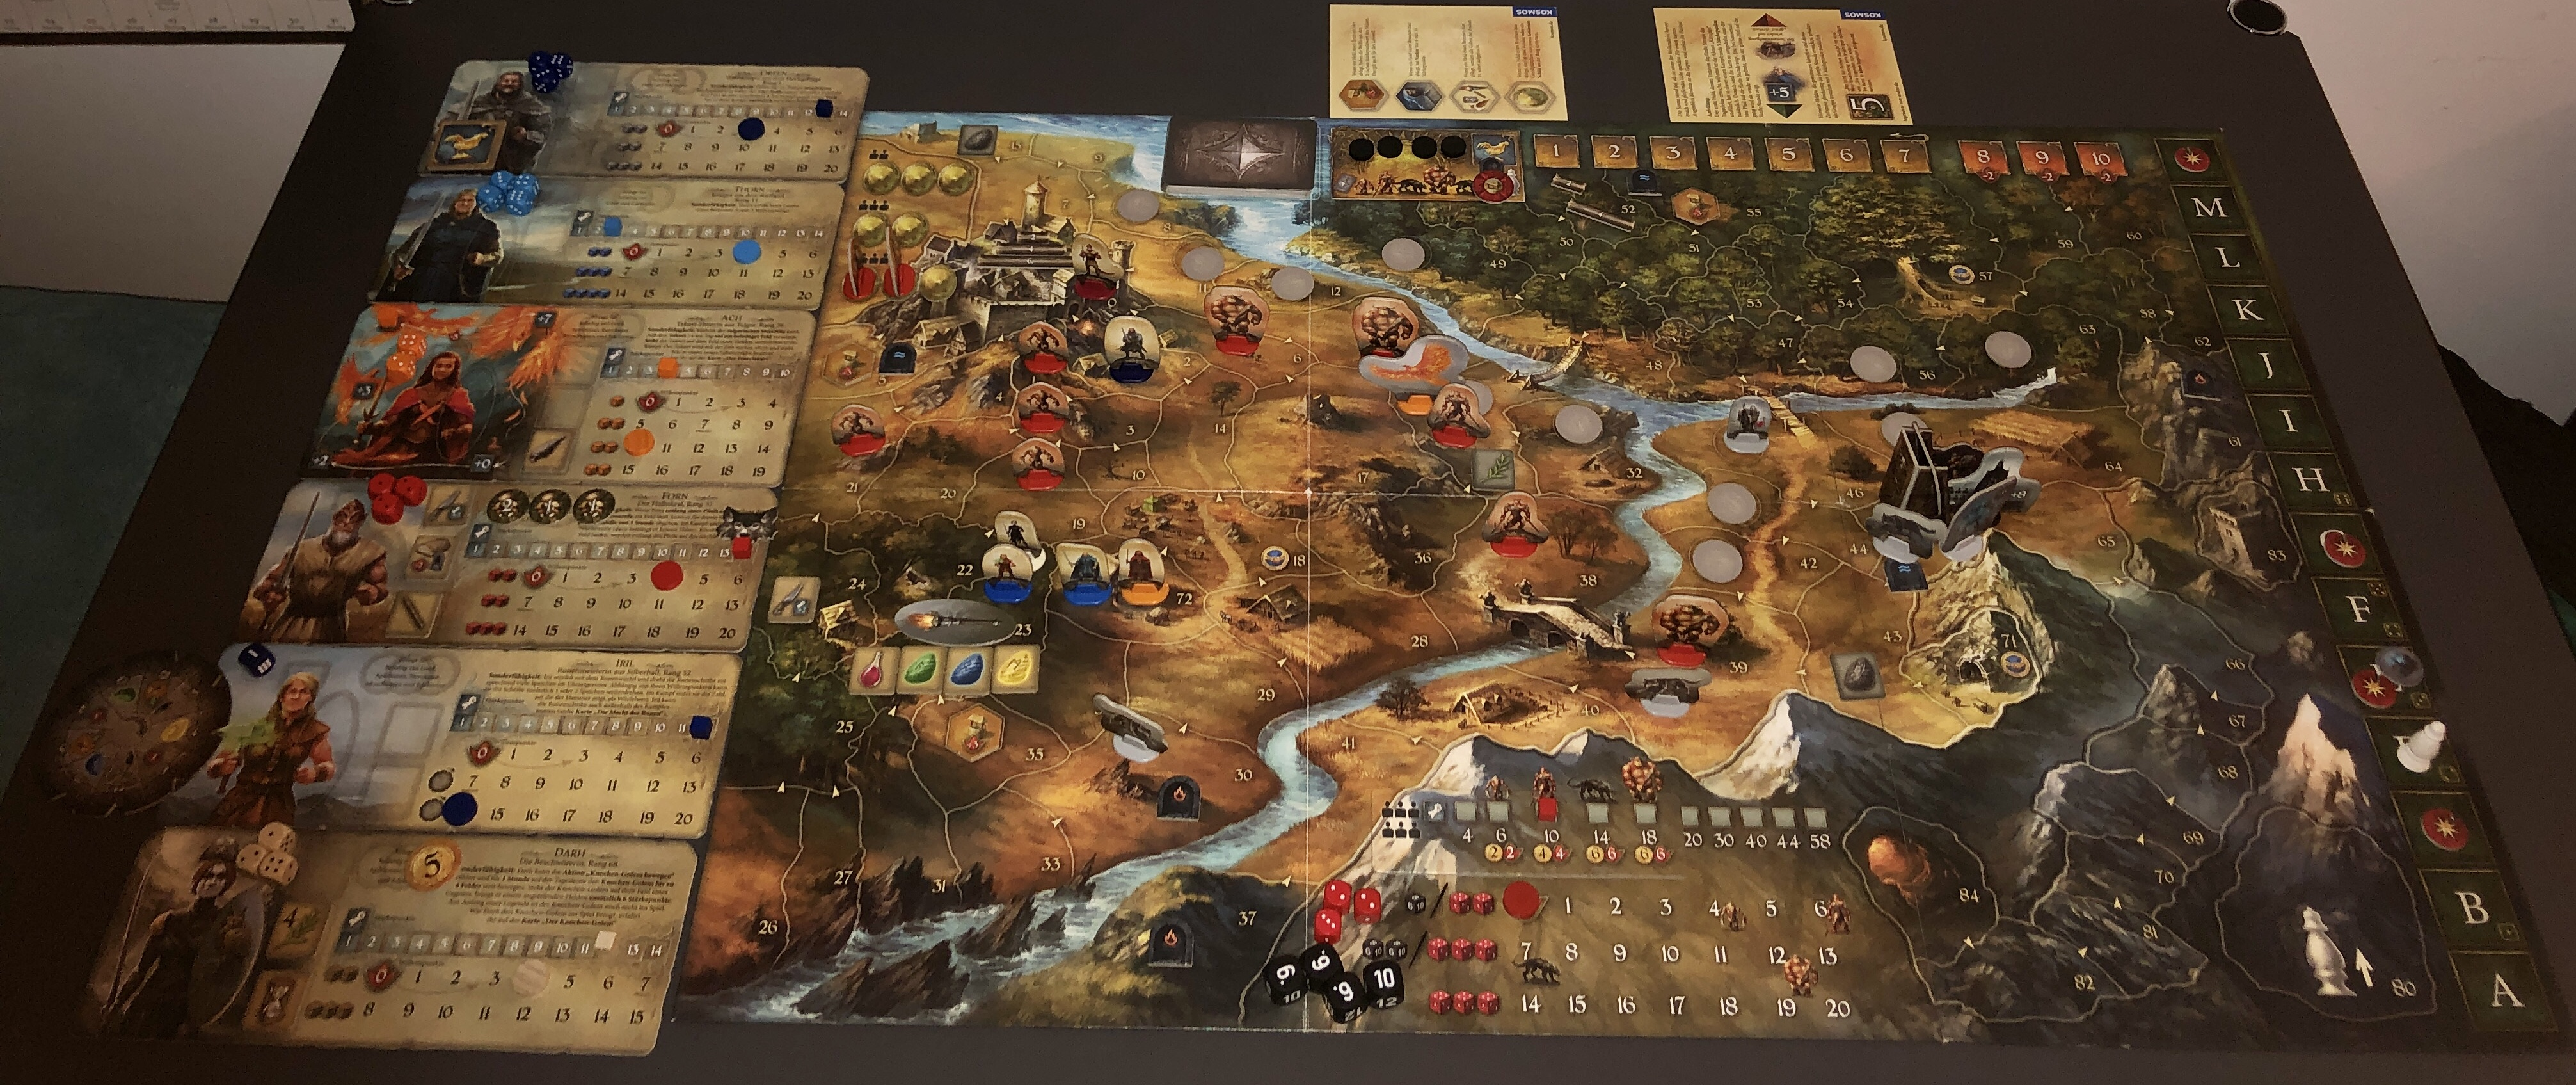
\includegraphics[width=\textwidth]{Das Erbe des Wunderkindes/Bilder/Tag 3 Anfang.jpg}

\textit{Anfang von Tag 3.}\bigskip


Das Tagesmotto dreht sich heute ganz ums Sammeln von Gold durch Vertreibung dunkler Kreaturen. Und darum, den Belagerungsturm mithilfe des Sternenschilds von der Rietburg fernzuhalten.



Forn nutzt die andorische Flöte. Der Würfel zeigt eine 6! Forns WP steigen auf 4 +6 = 10. Da Orfen auf 2 angrenzend zu 0 steht, steigen auch Orfens WP auf 3 +6 = 9.



Zug 1: Orfen läuft für 1 Stunde (Zeitstein von 0 auf 1) von 2 auf 6.



Zug 2: Thorn beendet seinen Tag. Thorn erhält das Sonnenaufgang-Plättchen.



Zug 3: Aćh passt (Zeitstein von 1 auf 2). Sie will gleich noch Turr besänftigen, wenn der Erzähler E erreicht.



Zug 4: Forn, der Wolfsfreund, wählt die Aktion "Wölfe bewegen". Rutan läuft für 1 Stunde (Zeitstein von 2 auf 3) von 39 auf 6.

Darh nutzt das Hadrische Stundenglas, um den Zeitstein von 3 zurück auf 0 zu schieben. Dann legt sie das Stundenglas auf 23 ab. Die kleinen Ablagefelder der lange wachen Helden dürften heute knapp werden.

Darh schickt die Eule mit den drei Runensteinen von 23 an Orfen.



Zug 5: Iril beendet ihren Tag bereits. Ausnahmsweise. ;)



Zug 6: Darh muss passen, da sie noch nicht weiß, wo die E-Kreaturen auftauchen werden. Darh wählt ihre Aktion "Knochen-Golem bewegen". Der Knochen-Golem läuft für 1 Stunde (Zeitstein von 0 auf 1) eine fröhliche Runde von 45 über 44/46/64 auf 45.



Zug 7: Orfen bekämpft den 6-Troll.

In Kampfrunde 1 (Zeitstein von 1 auf 2) hat Orfen einen Kampfwert von 13 SP +14 (Rutan) +10 (großer schwarzer Würfel) = 37.

Der 6-Troll hat einen Kampfwert von 18 SP +6 (Würfel) = 24.

Der Troll ist besiegt.

Belohnung: Orfens Gold steigt auf 0 +6 = 6.

Der Erzähler läuft auf E. Eine Legendenkarte wird ausgelöst. Der Knochen-Golem kommt zurück auf 80. Dafür erscheinen mehr Kreaturen im Südlichen Wald: Gor auf 22, Trolle auf 24 und 34. Und ein bösartiger Wardrak verlässt via 67 das Graue Gebirge.



Zug 8: \textit{Vorsicht! Brennt die Flamme des Takuri zu heiß, endet sein Lebenszyklus. Ein Glück, dass die tapfere Aćh ihn immer wieder beruhigen kann.} Aćh beruhigt Turr. Der Takuri-Marker sinkt von +7 auf +5. Aćhs WP sinken auf 10 -5 = 5.

Aćh beendet ihren Tag.



Zug 9: Forn, der Wolfsfreund, wählt die Aktion "Wölfe bewegen". Merla läuft für 1 Stunde (Zeitstein von 2 auf 3) von 30 auf 24.



Zug 10: Darh läuft für 1 Stunde (Zeitstein von 3 auf 4) von 23 auf 24. Darh nimmt das Messer von 24 auf.



Zug 11: Orfen läuft für 2 Stunden (Zeitstein von 4 auf 6) von 6 auf 16. Das 16-Nebelplättchen versteckte einen Stärkepunkt. Orfens SP steigen auf 13 +1 = 14.

Orfen findet ein 4er-Heilkraut. Er frischt die Eule auf. Orfens WP sinken auf 9 -3 = 6. Orfen schickt das 4er-Heilkraut mit der Eule an Darh.



Zug 12: Forn, der Wolfsfreund, wählt die Aktion "Wölfe bewegen". Rutan läuft für 1 Stunde (Zeitstein von 6 auf 7) von 6 auf 13.



Zug 13: Darh bekämpft den 24-Troll.

In Kampfrunde 1 (Zeitstein von 0 auf 1) hat Darh einen Kampfwert von 12 SP +14 (Merla) +6 (Würfel) = 32.

Der 24-Troll hat einen Kampfwert von 18 SP +6 (Würfel) = 24.

Die WP des 24-Trolls sinken auf 12 -8 = 4.

In Kampfrunde 2 (Zeitstein von 1 auf 2) hat Darh einen Kampfwert von 12 SP +14 (Merla) +3 (Würfel) = 29.

Der 24-Troll hat einen Kampfwert von 18 SP +4 (Würfel) = 22.

Der 24-Troll ist besiegt.

Belohnung: Darhs Gold steigt auf 5 +6 = 11.

Darh beschwört ihren Knochen-Golem. Er wird samt Troll auf 36 eingewürfelt. Das Golem-Symbol kommt auf I.

Der Erzähler läuft auf F.



Zug 14: Orfen bekämpft den 16-Skral.

In Kampfrunde 1 (Zeitstein von 2 auf 3) hat Orfen einen Kampfwert von 14 SP +7 (Turr) +10 (großer schwarzer Würfel) = 31.

Der 16-Skral hat einen Kampfwert von 10 SP +2 (Würfel) = 12.

Der 16-Skral ist besiegt.

Belohnung: Orfens Gold steigt auf 6 +4 = 10.

Der Erzähler läuft auf G. \textit{Nun sieht der Takuri Orfen noch einmal an, und in einem kurzen Augenblick rotglühenden Feuers beendet er sein Leben, so wie er es schon so oft beendet hat.} Er sinkt auf +0.

In dieser Partie denken die Helden auf G über Gildas Lieder nach. Da gleich zwei Helden auf 72 stehen (bzw. liegen), lesen wir direkt auf der Hinweiskarte "Gildas Lied" weiter. Gilda singt den schlafenden Helden das Lied von Nehal und verweist auf den Krallenfelsen (30). Doch die Zeit drängt! Auch Varkur ist auf der Suche nach dem Sternenschild. Haben wir ihn bis I (zwei Erzählerbewegungen) nicht gefunden, wird er ihn triumphierend an sich reißen!



Zug 15: Forn wählt die Aktion "Wölfe bewegen". Lonas läuft für 1 Stunde (Zeitstein von 3 auf 4) von 45 auf 38.



Zug 16: Darh läuft für 3 Stunden (Zeitstein von 4 auf 7) von 24 auf 30. Sie untersucht den Krallenfelsen und erkennt ... 30 +10 +8 = 48!

Mag dies die Stelle sein, an welcher der diebische Rudnar einst während der Trollkriege den gestohlenen Sternenschild versteckte?



Zug 17: Orfen läuft für 1 Stunde (Zeitstein von 0 auf 1) von 16 auf 38.



Zug 18: Forn läuft für 4 Stunden (Zeitstein von 1 auf 5) von 0 auf 48. Triumphierend nimmt er den Sternenschild auf. Varkur dampft wutschnaubend davon.

Forn nutzt den Sternenschild, um das Brunnen-Symbol abzudecken. Dann bewegt sich der Belagerungsturm beim nächsten Sonnenaufgang nicht.



Zug 19: Darh läuft für 1 Stunde (Zeitstein von 5 auf 6) von 30 auf 29.



Zug 20: Orfen bekämpft den 38-Skral.

In Kampfrunde 1 (Zeitstein von 6 auf 7) hat Orfen einen Kampfwert von 14 SP +14 (Lonas) +10 (Würfel) = 38.

Der 38-Skral hat einen Kampfwert von 10 SP +5 (Würfel) = 15.

Der 38-Skral ist besiegt.

Belohnung: Orfens Gold steigt auf 10 +4 = 14.

Der Erzähler läuft auf H.



Zug 21: Forn läuft für 2 WP (Forns WP sinken auf 10 -2 = 8) von 48 auf 13. Das 13-Nebelplättchen versteckte 1 Gold. Forns Gold steigt auf 4 +1 = 5.



Zug 22: Darh läuft für 1 Stunde (Zeitstein von 0 auf 1) von 29 auf 28.



Zug 23: Orfen beendet seinen Tag.



Zug 24: Forn bekämpft den 13-Troll.

In Kampfrunde 1 (Zeitstein von 1 auf 2) hat Forn einen Kampfwert von 14 SP +14 (Rutan) +12 (Würfel) = 40.

Der 13-Troll hat einen Kampfwert von 18 SP +5 (Würfel) = 23.

Der 13-Troll ist besiegt.

Belohnung: Forns Gold steigt auf 5 +6 = 11.

Der Erzähler läuft auf I. Der Knochen-Golem kehrt zurück auf 80.



Zug 25: Darh läuft für 1 Stunde (Zeitstein von 2 auf 3) von 28 auf 36.



Zug 26: Forn, der Wolfsfreund, wählt die Aktion "Wölfe bewegen". Lonas läuft für 1 Stunde (Zeitstein von 3 auf 4) von 38 auf 36. Der Wolf, der schwarze Wolf, hatte Darhs Witterung aufgenommen. ;)



Zug 27: Darh bekämpft den 36-Troll.

In Kampfrunde 1 (Zeitstein von 4 auf 5, das Licht der fünften Stunde wird ausgelöst) hat Darh einen Kampfwert von 12 SP +14 (Lonas) +5 (Licht der fünften Stunde) +4 (Würfel) = 35.

Der 36-Troll hat einen Kampfwert von 18 SP +5 (Würfel) = 23.

Der 36-Troll ist besiegt.

Belohnung: Darhs Gold steigt auf 11 +6 = 17.

Darh beschwört ihren Knochen-Golem, schon zum zweiten Mal bei diesem Troll. Der Knochen-Golem wird samt Troll auf 32 eingewürfelt. Das Golem-Symbol kommt auf M.

Der Erzähler läuft auf J.



Zug 28: Forn, der Wolfsfreund, wählt die Aktion "Wölfe bewegen". Merla läuft für 1 Stunde (Zeitstein von 5 auf 6) von 24 auf 72.



Zug 29: Darh wählt ihre Aktion "Knochen-Golem bewegen". Der Knochen-Golem läuft für 1 Stunde (Zeitstein von 6 auf 7) von 32 auf 72.



Zug 30: Forn beendet seinen Tag.



Zug 31: Darh beendet ihren Tag.\bigskip


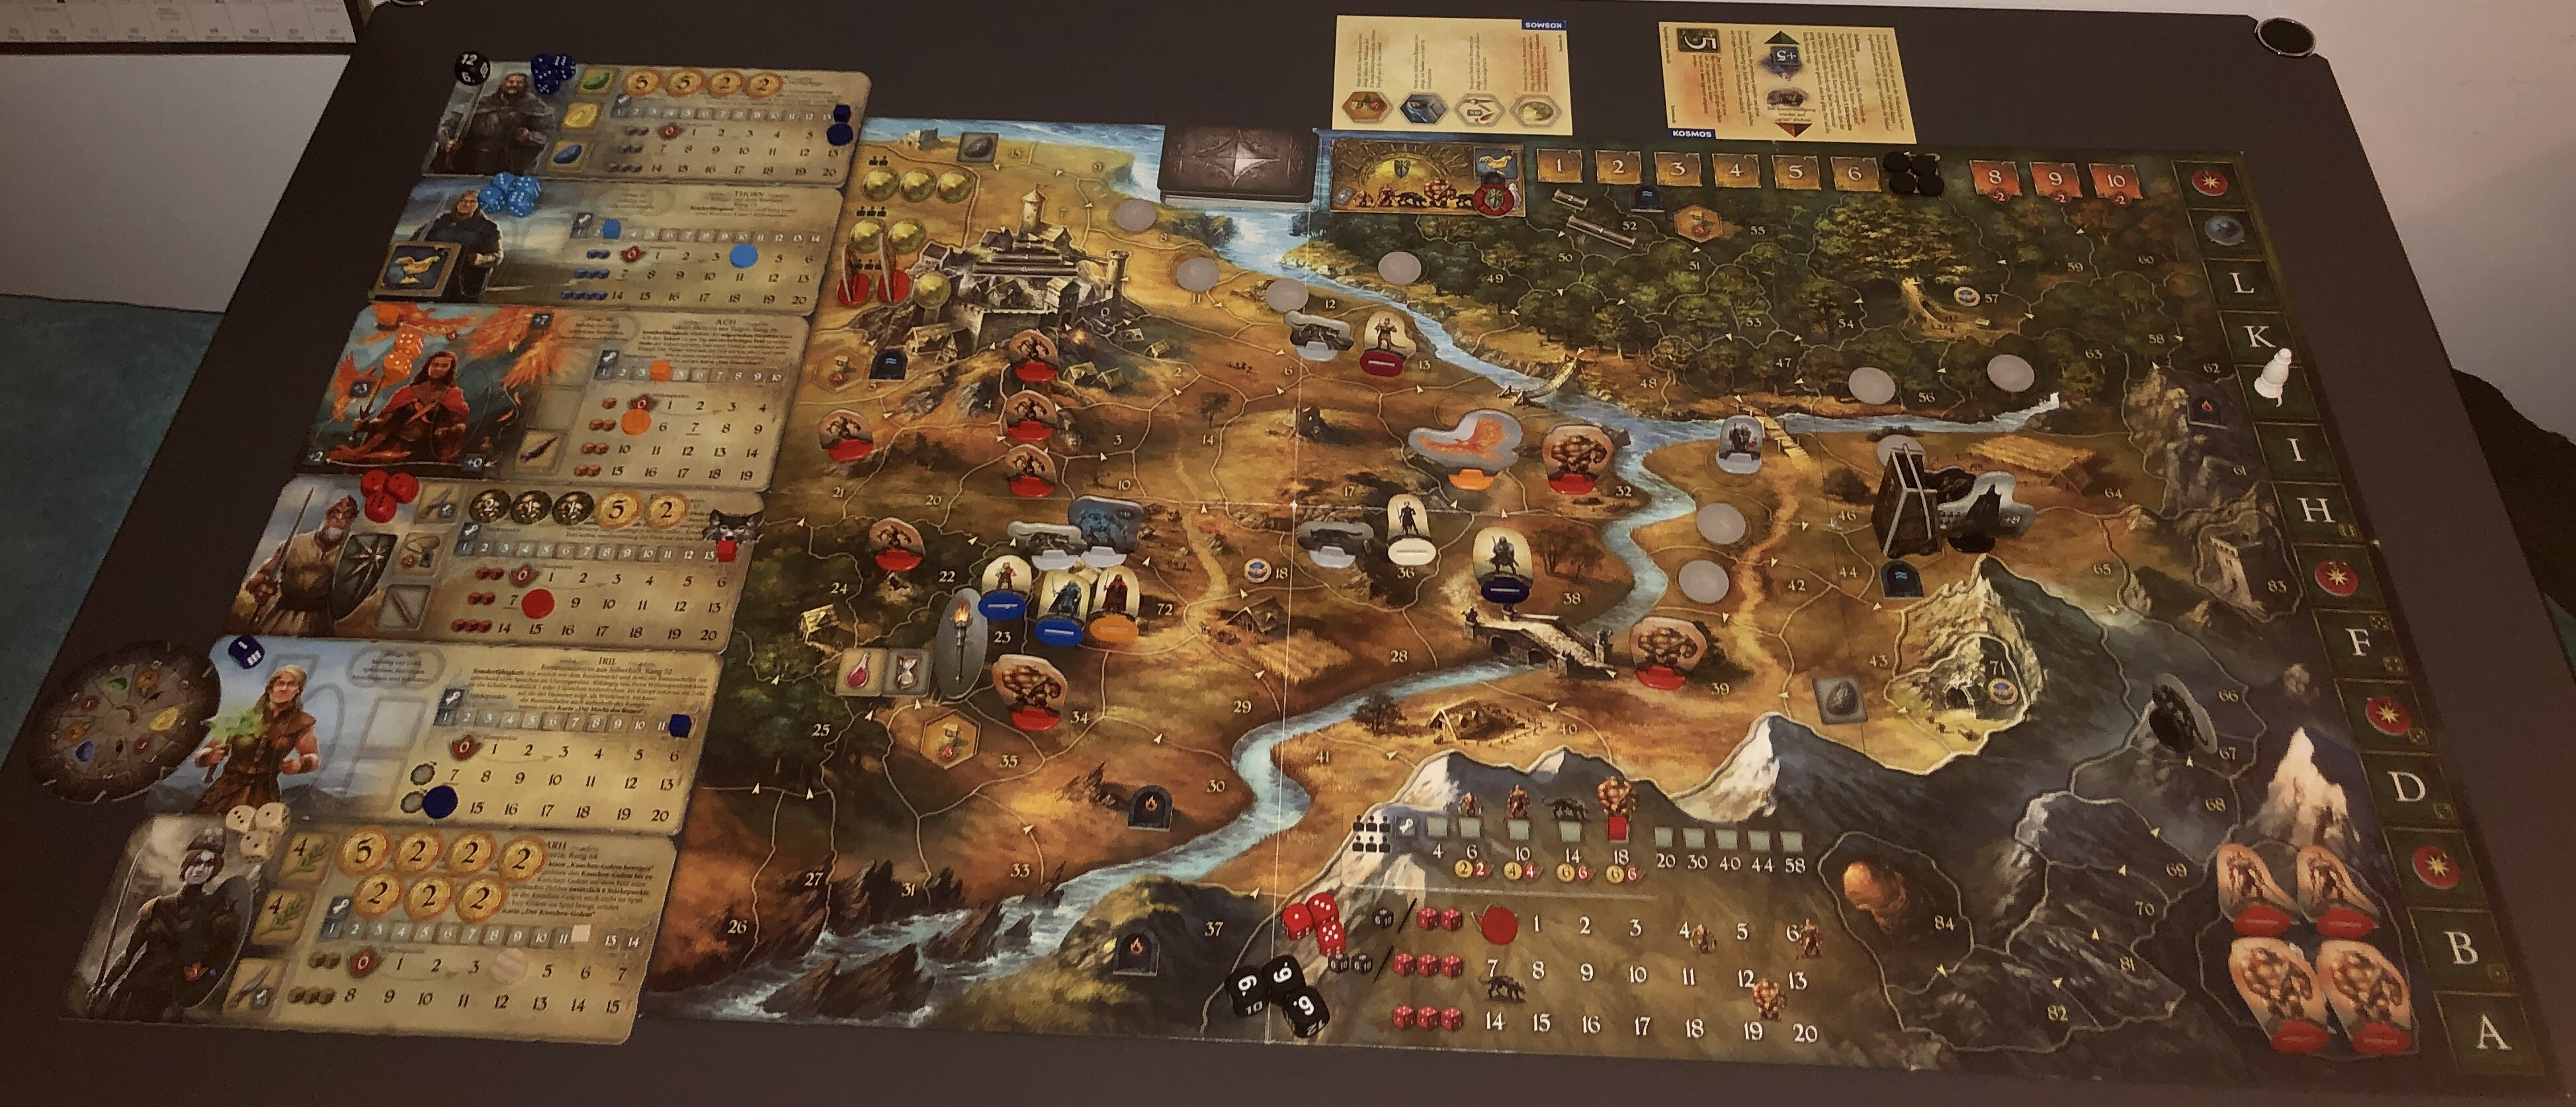
\includegraphics[width=\textwidth]{Das Erbe des Wunderkindes/Bilder/Tag 3 Ende.jpg}

\textit{Ende von Tag 3.}

\newpage
\section{Tag 4}


Sonnenaufgang:

Weiße Ereigniskarte 1 wird ausgelöst. Orfen setzt einen Zeitstein von 0 auf 2, um die Kampfaxt zu erhalten.

Kreaturen laufen, davon ein Gor auf den letzten freien goldenen Schild.

Die Brunnen werden wegen des Sternenschilds nicht aufgefrischt. Der Belagerungsturm bleibt auf somit 45 stehen.

Der Erzähler läuft auf K.\bigskip

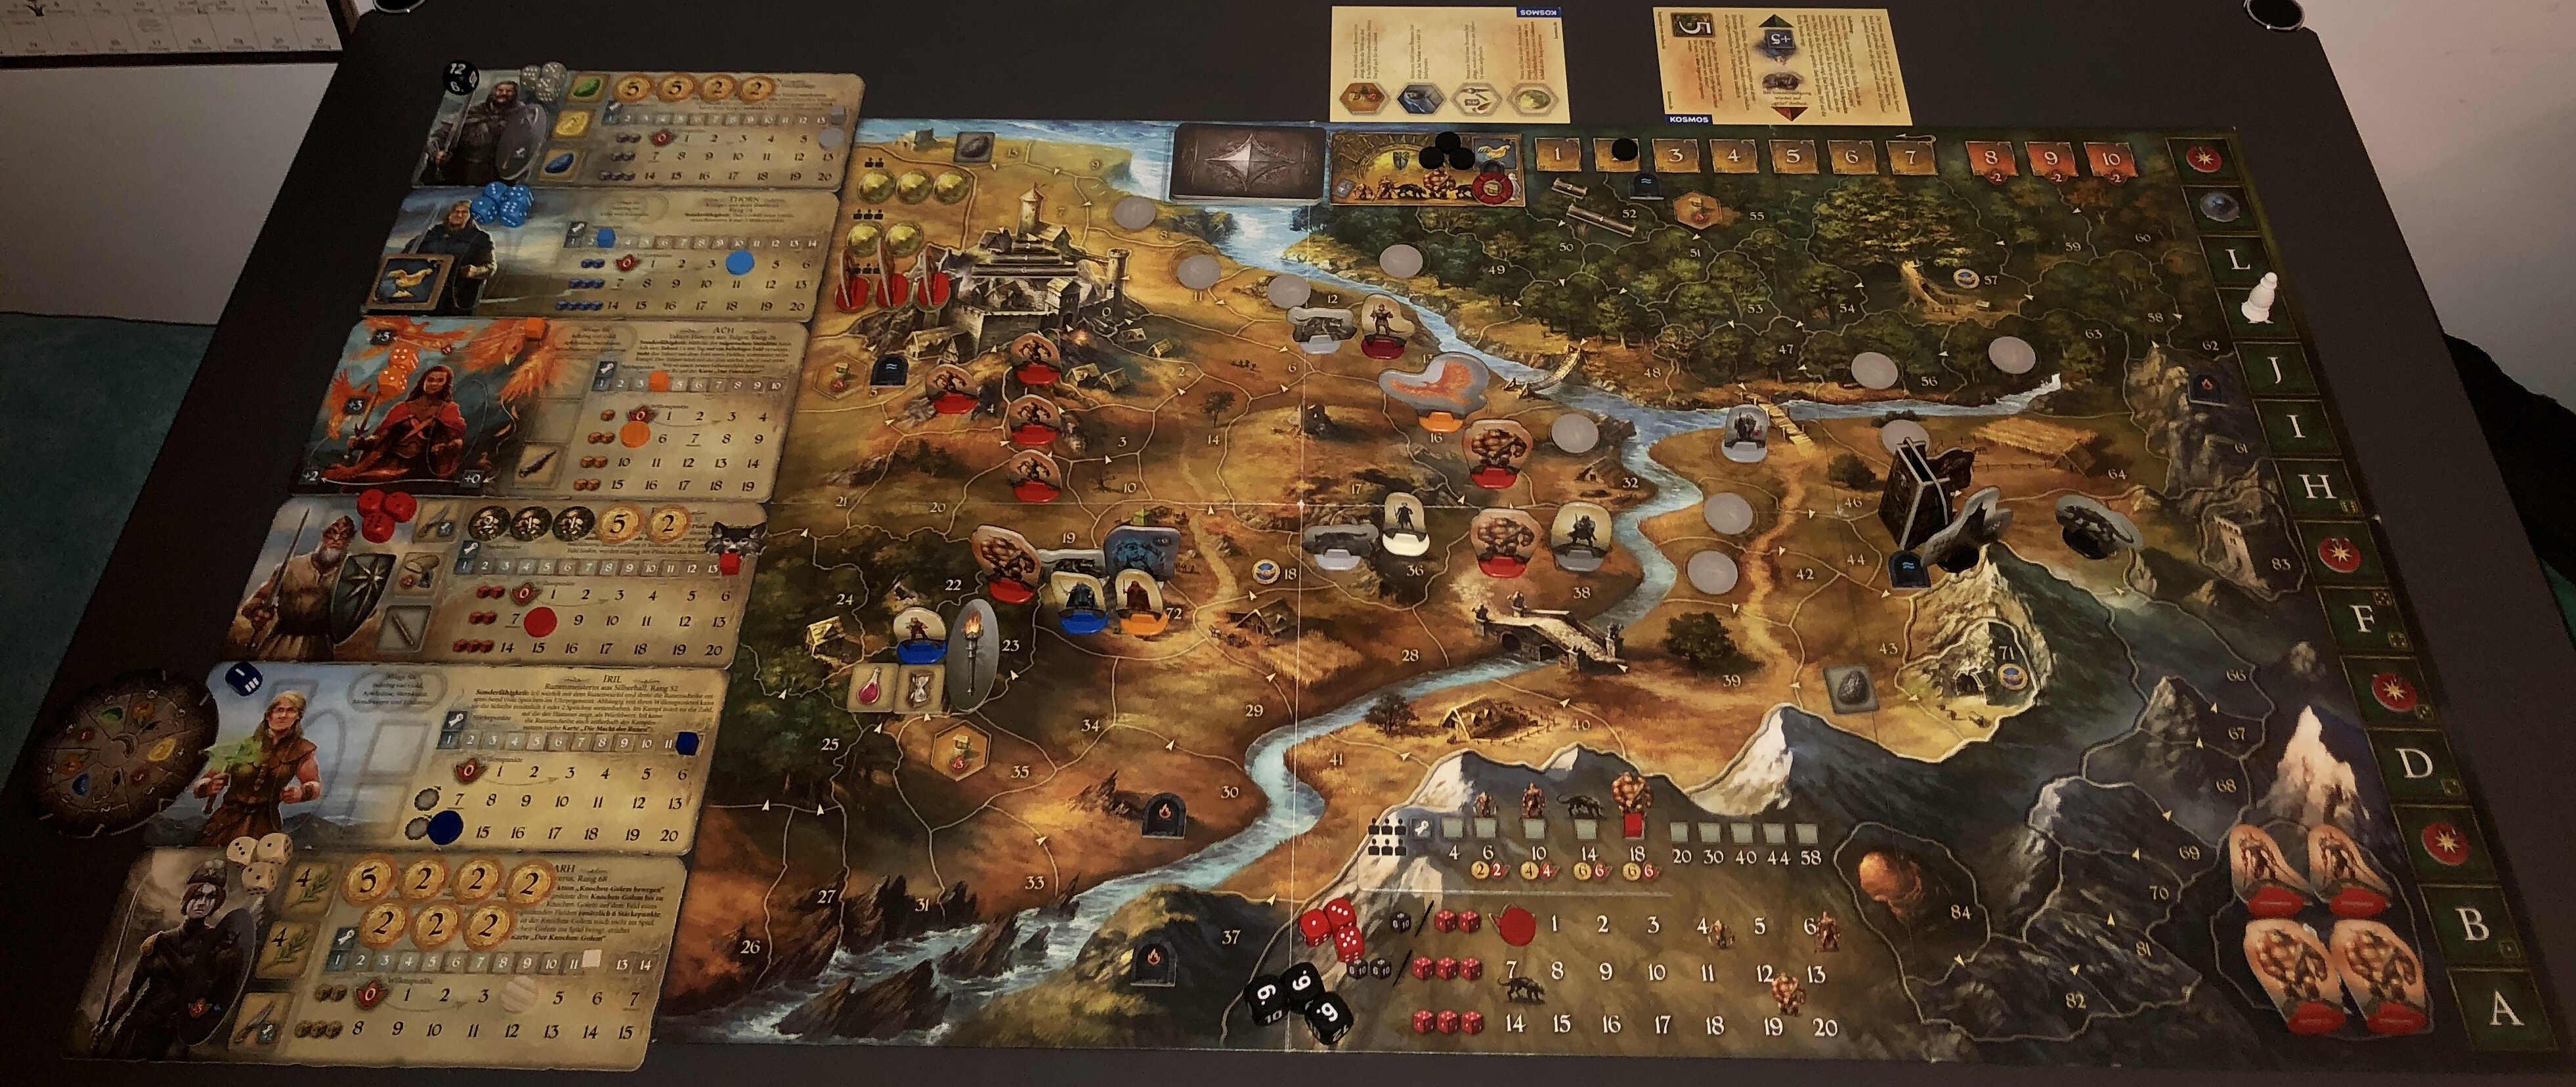
\includegraphics[width=\textwidth]{Das Erbe des Wunderkindes/Bilder/Tag 4 Anfang.jpg}

\textit{Anfang von Tag 4.}

\textit{Korrekturen: Das Licht der fünften Stunde, Darhs Eule und Forns Flöte sollten alle bereits wieder aufgefrischt sein. Hach, gegen Ende schleicht sich wieder der Fehlerteufel ein :(}\bigskip


Iril nimmt die Fackel von Cavern, das Hadrische Stundenglas und den Trank der Hexe von 23 auf.

Iril nutzt die Fackel von Cavern, um den Troll von 23 auf 72 zu scheuchen.

Aćh nutzt ihre tulgorische Steinflöte. Turr fliegt von 16 auf 72.

Jawohl, der entscheidende Kampf wird gegen einen gewöhnlichen Troll und nicht gegen den Belagerungsturm sein. :D



Zug 1: Thorn passt (Zeitstein von 2 auf 3). Jemand muss auf 72 warten, um Forns Gold entgegenzunehmen, und dieser jemand ist er.

Iril nutzt das Hadrische Stundenglas, um den Zeitstein von 3 zurück auf 0 zu schieben.



Zug 2: Aćh läuft für 1 Stunde (Zeitstein von 0 auf 1) von 72 auf 18.



Zug 3: Forn läuft für 3 Stunden (Zeitstein von 1 auf 4) von 13 auf 72.

Thorn erhält Forns Gold (11, davon 4 Waldpilze).



Zug 4: Iril läuft für 1 Stunde (Zeitstein von 4 auf 5) von 23 auf 72.



Zug 5: Darh läuft für 1 Stunde (Zeitstein von 5 auf 6) von 36 auf 18.

Darh kauft sich 2 SP. Darhs Gold sinkt auf 17 -4 = 13.



Zug 6: Orfen läuft für 2 Stunden (Zeitstein von 6 auf 8, Orfens WP sinken auf 6 -2 = 4) von 38 auf 18.

Orfen kauft sich einen Helm. Orfens Gold sinkt auf 14 -2 = 12.

Aćh erhält den Rest von Orfens Gold. Aćhs Gold steigt auf 0 +12 = 12.

Aćh kauft sich 6 SP. Aćhs Gold sinkt auf 12 -12 = 0. Aćhs SP steigen auf 4 +6 = 10.



Zug 7: Thorn läuft (mit Forns 11 Gold) für 1 Stunde (Zeitstein von 0 auf 1) von 72 auf 18.

Thorn erhält Darhs Gold. Thorns Gold steigt auf 11 +13 = 24.

Thorn kauft sich 11 SP und einen Helm. Thorns Gold sinkt auf 24 -22 -2 = 0. Thorns SP steigen auf 3 +11 = 14.

Alle Stärkeleisten sind voll! :D



Zug 8: Aćh läuft für 1 Stunde (Zeitstein von 1 auf 2) von 18 auf 72.



Zug 9: Forn, der Wolfsfreund, wählt die Aktion "Wölfe bewegen". Rutan läuft für 1 Stunde (Zeitstein von 2 auf 3) von 13 auf 72. Lonas läuft für 1 Stunde (Zeitstein von 3 auf 4) von 36 auf 72.

Alle Unterstützer stehen bereit! :D



Zug 10: Iril wählt ihre Aktion "Runen befragen", um sich optimal auf den Kampf einzustimmen.

In Stunde 5 zeigt der Runenwürfel eine 1. Iril dreht die Runenscheibe um 1 +1 = 2 Speichen auf den 2-Brunnen. Es gibt zwar keine geleerten Brunnen aufzufrischen, aber dafür ist sie perfekte 3 Speichen vom Kampfwert 5 entfernt.



Zug 11: Darh läuft für 1 Stunde (Zeitstein von 5 auf 6) von 18 auf 72.



Zug 12: Orfen läuft für 1 Stunde (Zeitstein von 6 auf 7) von 18 auf 72.



Zug 13: Thorn läuft für 1 Stunde (Zeitstein von 0 auf 1) von 18 auf 72.

Alle Helden sind in Position! :P



Die andorische Flöte wird an unsere Flötenspielerin Aćh übergeben. Aćh spielt die Flöte. Der Würfel zeigt eine 4. Aćhs WP steigen auf 5 +4 = 9. Irils WP steigen auf 14 +4 = 18. Darhs WP steigen auf 4 +4 = 8. Orfens WP steigen auf 4 +4 = 8. Thorns WP steigen auf 4 +4 = 8. Forns WP steigen auf 8 +4 = 12.

Forn teilt sein Brot. Alle Helden erhalten 6x2 = 12 WP.

Alle Willensleisten sind voll! :D



Die Gegenstände werden ein bisschen umverteilt, aber nicht groß.

Aćh: 10 SP, 19 WP, drei Runensteine, Eule

Iril: 12 SP, 20 WP, Trank der Hexe (den Iril auf ihren Speichenwert anwenden darf\footnote{Aus der Taverne, "Magische Helden und ein paar allgemeine Fragen
": [Giftknödel:] Irils Speichenwert entspricht einem normalen Würfelwert. Demnach darf sie den Trank der Hexe darauf verwenden.}), Hadrisches Stundenglas, Fackel von Cavern

Darh: 14 SP, 20 WP, Helm, 2x Messer

Orfen: 14 SP, 20 WP, Helm, Kampfaxt

Thorn: 14 SP, 20 WP, Helm, andorische Flöte und tulgorische Steinflöte, warum auch nicht.

Forn: 14 SP, 20 WP, 2x 4er-Heilkraut, Sternenschild\bigskip



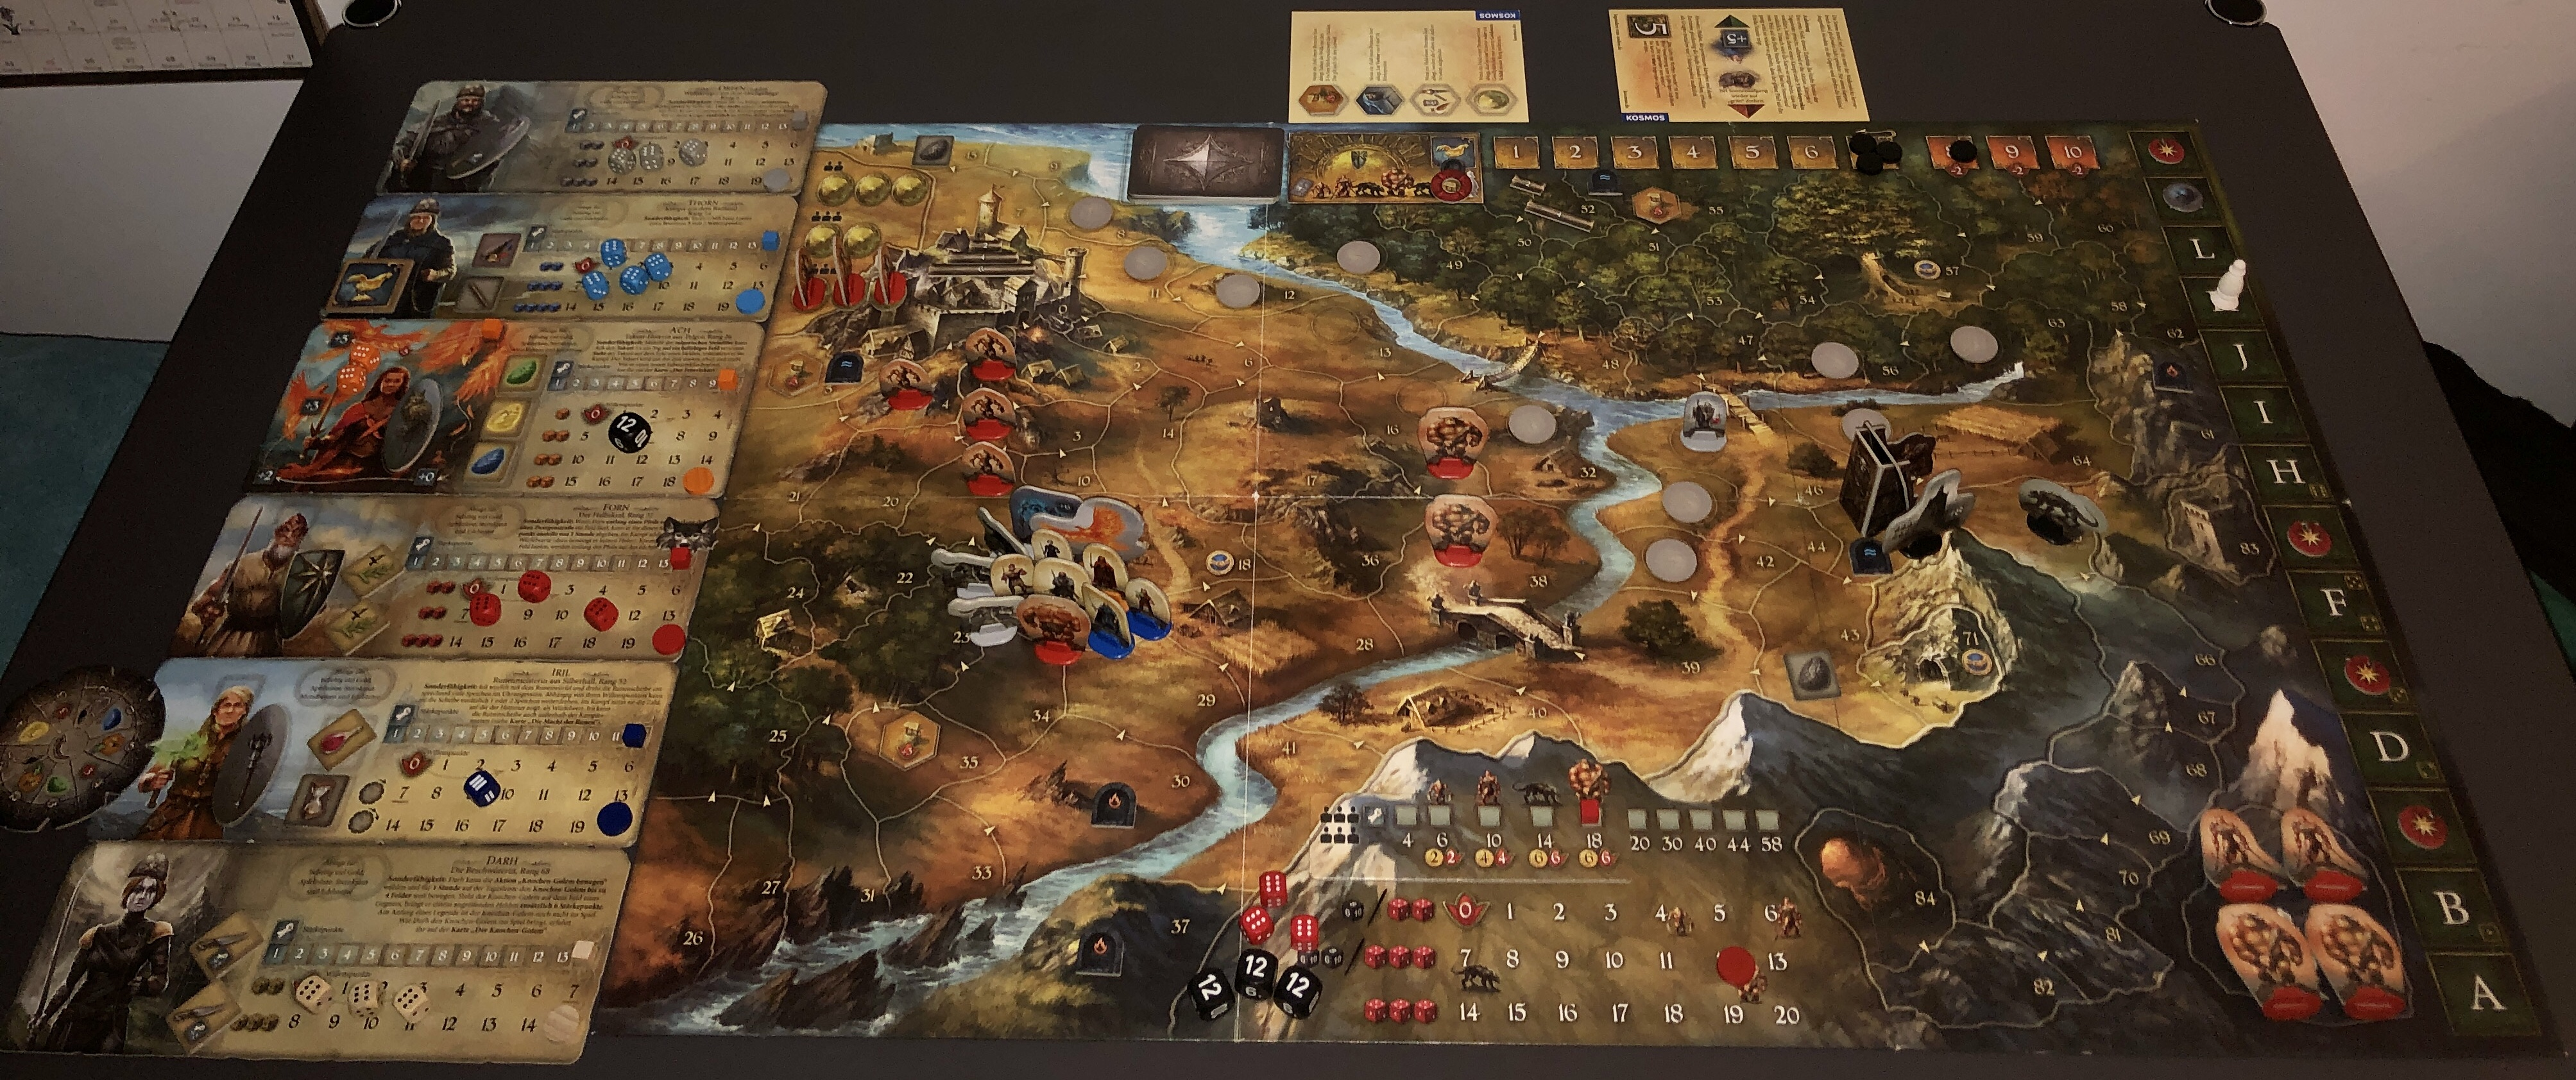
\includegraphics[width=\textwidth]{Das Erbe des Wunderkindes/Bilder/Tag 4 Endkampf.jpg}

\textit{Trollkampf an Tag 4. Schräg liegende Gegenstände werden soeben verbraucht.}\bigskip

Zug 14: Aćh lädt alle Helden zum gemeinsamen Kämpfen gegen den 72-Troll ein.

In Kampfrunde 1 (Zeitstein von 1 auf 7, das Licht der fünften Stunde wird ausgelöst) haben die Helden einen Kampfwert von 10 SP (Aćh) +14 SP (Forn) +12 SP (Iril) +14 SP (Darh) +14 SP (Orfen) +7 (Orfens Trollbonus) +14 SP (Thorn) +14 (Lonas) +14 (Rutan) +14 (Merla) +7 (Turr) +6 (Knochen-Golem) +5 (Licht der fünften Stunde) +12 (Aćhs großer schwarzer Würfel) +18 (Forns Pasch) +8 (2 Heilkräuter) +5 (Iril dreht ihre Runenscheibe um 3 Speichen auf den 5-Brunnen) +5 (Trank der Hexe) +18 (Darhs Pasch) +4 (2 Messer) +18 (Orfens Pasch) +4 (Kampfaxt) +24 (Thorns Pasch) = 261.\bigskip



Ich wiederhole dies gern noch etwas lauter:

{\Large Kampfwert 261!}

Ganz legal (sofern nicht verrechnet)! Und klar, die vielen 6er-Päsche sind sehr unwahrscheinlich, aber die ganzen restlichen Kampfpunkte sind gar nicht so unrealistisch zu erreichen!\bigskip



Der 72-Troll ist natürlich besiegt, der Erzähler läuft auf L und da die Fürstenaufgabe schon längstens erfüllt ist, müssten wir nun nur noch den Belagerungsturm besiegen gehen und könnten die Legende sogar noch gewinnen! :P\bigskip



Falls es heute nicht mehr für den Belagerungsturm reichen sollte, können wir immer einfach...

... den Belagerungsturm mit der zweiten Seite des Sternenschilds am Laufen hindern, ...

... Forn mit der Fackel von Cavern zur Burg flitzen lassen, für 1 Stunde von 0 nach 5 hoppeln, den 5-Brunnen den Wunschbrunnen opfern und sich aufgefrischte Gaben der Andori wünschen, danach für 1 Stunde von 5 nach 4 laufen und den 4-Gor mit der Fackel ein Feld zurückscheuchen, damit am nächsten Sonnenaufgang nur der 1-Gor in die Burg läuft, ...

... einen Helden für 2 Stunden nach 35 hoppeln lassen, den 35-Brunnen den Wunschbrunnen opfern und sich einen freien goldenen Schild für den 1-Gor wünschen ...

... und schon haben unsere tapferen Helden auf M noch einen ganzen Tag Zeit, den Belagerungsturm zu erreichen und zu demolieren. So geht das!






\newpage
\section{Verbesserungspotential}







Zum Nachtmodus:



Ich wünschte, ich hätte mir die Legendenkarte zum Heldenlager rechtzeitig nochmals durchgelesen. Der Nachtmodus hätte hier wirklich tolles Potential gehabt.

Im Sonnenaufgang von Tag 1 auf Tag 2 (bzw. in der Dämmerung von Nacht 1 auf Nacht 2) erhalten alle Helden im Heldenlager je 1 Stärkepunkt. Potentielle +6 SP sind schon sehr praktisch, aber es kommt noch besser: In der Dämmerung von Nacht 3 auf Nacht 4 dürfen alle Helden im Heldenlager untereinander SP und WP tauschen. Das hätte uns erlaubt, Irils volle Stärkeleiste am Ende auch noch mit Thorns leerer Leiste zu tauschen und Irils Stärkeleiste ein fünftes Mal mit Runenmagie hochzupowern. Dann hätten wir erheblich weniger Gold sammeln müssen.

Den endgültigen Kampfwert hätte das allerdings nicht verbessert.\bigskip







Zu Orfen:



Wenn man irgendwie den Belagerungsturm daran hinderte, die 80er-Felder zu verlassen (was bedingen würde, am Tag seines Auftauchens den Erzähler von C auf mindestens G zu pushen und sofort den Sternenschild zu finden, oder aber beinahe alle Kreaturen vom Spielplan zu räumen) und wenn man danach irgendwie alle Helden und Begleiter mit vollen Stärkeleisten und voller Ausrüstung auf ein 80er-Feld mit Belagerungsturm darauf brächte, könnte man den Endkampf dort stattfinden lassen.

Da man explizit nicht den Belagerungsturm, sondern den ihn herumschiebenden Troll bekämpft, sollte Orfen dann einen Stärkebonus von +8 statt +7 kriegen können und den maximalen Kampfwert von obigem Spielbericht um 1 Punkt übertreffen.

Ob das wirklich möglich ist, steht allerdings noch in den Sternen. Eventuell könnte man einen Bauern der Mini-Erweiterung "Die Taverne von Andor" opfern, um den Erzähler von B auf A zurückzusetzen und so einen Tag zu gewinnen, ehe der Belagerungsturm erscheint. Dann dürfte es bei den goldenen Schilden der Rietburg jedoch knapp werden.



Alternativ könnte man auch versuchen, einen gewöhnlichen Troll auf ein 80er-Feld zu befördern. Doch da Orfen mit Helm auf dem Trollfeld stehen muss, und da Feld 83 für Trolle unerreichbar ist (selbst mit Ijsdurs Eisbrücken\footnote{Aus der Taverne, "Einige Fragen zu den Magischen Helden": [Doro:] Selbst der magische Ijsdur kann mit der Fackel eine Kreatur nur auf ein wirklich angrenzendes Feld versetzen. }), würde das bedingen, einen gewöhnlichen Troll (evtl. durch Darh auf Feld 66 eingewürfelt) mit Sternenschild, Zwergenseil und/oder dem Geisterfeuer des Dunklen Tempels tagelang am Laufen zu hindern und mit der Fackel von Cavern immer näher in Richtung 81 schubsen (wobei man immerhin einmal einen Brunnen opfern könnte, um sich eine Auffrischung der Gaben der Andori zu wünschen und somit zwei Fackelnutzungen an diesem Tag zu kriegen).

Ob das wirklich möglich ist, steht allerdings ebenfalls noch in den Sternen. Ich bin mir nicht einmal sicher, ob es regeltechnisch erlaubt wäre, mit Zwergenseil gefangene oder hingelegte Kreaturen durch die Fackel von Cavern zu bewegen.\bigskip







Zu Bragor:



In meinen ersten Theorien zum maximalen Kampfwert war Bragor noch mit von der Partie, damit er sich von Iril jeweils an einem Brunnen hochpowern lassen konnte. Das Witzige daran wäre, dass man dann mit dem letzten Lagerfeuer (oder dem Heldenlager aus dem Nachtmodus) gleichzeitig zwei Helden hätte vollpowern können. In Kombination der beiden Lager oder eines Lagers mit dem 2x SP-Tauschen des Bruderschilds hätte man somit am Ende keinen einzigen Stärkepunkt mit Gold kaufen müssen.

Aber Aćhs maximale 10 SP +7 (Turr) +12 (schwarzer Würfel) = 29 sind eindeutig besser als Bragors maximale 14 SP +12 (schwarzer Würfel) = 26, darum wurde des Taren große Heldentafel gegen der Takuri-Hüterin große Heldentafel eingetauscht.\bigskip







Zu Iril-Alternativen:



Aktuell basiert unsere Strategie zum Füllen der Stärkeleisten hauptsächlich auf Irils Runenscheibe. Iril ist also zwingend mit von der Partie. Im Endkampf steuert Iril 12 SP +5 (Speiche) + 5 (TdH) = 22 bei. Wenn es uns gelänge, alternative Strategien zum Füllen der Stärkeleisten zu finden, könnten wir Iril vielleicht durch einen noch ein klein wenig stärkeren Helden ersetzen.



Kram kann auf Feld 71 mit Gold 1:1 SP kaufen. Genau wie Iril kann auch er einfacher generierte SP über Bruderschild, letztes Lagerfeuer und Heldenlager (Nachtmodus) mit anderen Helden tauschen. Vielleicht ist es irgendwie möglich, genügend Gold zu sammeln, damit Kram statt Iril von der Partie sein könnte.

Falls jemand sich daran versuchen will, könnte die Mini-Erweiterung "Koram, der Gor-Häuptling" helfen. Solange Koram im Spiel ist, haben Gors zwar die SP von Skralen, aber auch ihre Belohnung.

Kram würde im Endkampf maximal 14 SP +6 (Würfel) +6 (TdH, ist ja kein Helm mehr übrig) = 26 liefern, also ganze 4 Punkte besser als Iril.



Noch besser wäre es natürlich, Kheela statt Iril oder Kram antreten zu lassen. Kheela hat im Endkampf maximal 14 SP +7 (Wassergeist-Würfel) +7 (TdH) = 28, ganze 6 Punkte besser als Iril.

Ich habe aber keine Ahnung, wie man ohne Zwergentricks alle Stärkeleisten (fast) vollmachen will.

Ich studierte eine Zeit lang an einem möglichen Loop mit der Mini-Erweiterung "Die Magie von Choranat" herum, bei der zwei Helden abwechslungsweise alleine eine viel stärkere Kreatur (z.B. einen Troll) angriffen und den Kampf nach der ersten Kampfrunde jeweils wieder abbrächen. Der erste Held hätte nur 1 SP und würde immer wieder auf 0 WP fallen, ohne davon wirklich betroffen zu sein (er könnte so sogar beliebig viele Überstunden machen), während der zweite Held jeweils einen Schild vom Barz-Bannfeuer erhalten würde, um sich vor dem WP-Verlust zu schützen, und immer beim Ijsdur-Bannfeuer 1 SP erhalten würde.

Glücklicherweise las ich die Mini-Erweiterung nochmals genau durch und sah das kleingedruckte "eignet sich nicht für das Spiel mit 5 und 6 Helden", ehe ich noch länger versucht hätte, diesen Loop hier umzusetzen.

Nichtsdestotrotz: 1 SP pro 4 Stunden zu generieren, ist wirklich nicht schlecht, und der Loop könnte im Spiel mit 4 oder weniger Helden gut funktionieren, was die Mini-Erweiterung in meinen Augen gleich noch ein Stückchen mehr OP macht. ;)\bigskip







Zu Kirr:



Kirr könnte maximal 14 SP +6 (Zeitstein auf 10) +6 (Würfel) +6 (TdH) = 32 liefern, also satte 10 Punkte mehr als Iril.

Und selbst wenn wir bei der Iril-Strategie bleiben, wäre Kirr mit 14 SP +6 (Zeitstein auf 10. Stunde) +12 (schwarzer Würfel) = 32 Kampfpunkten um ganze 3 Punkte besser als Aćhs 10 SP +7 (Turr) +12 (schwarzer Würfel) = 29.

Wir sollten also Aćh durch Kirr ersetzen.



Die Frage, ob Kirr im Grundspiel (und den Erweiterungen) problemlos gespielt werden kann, würde ich mit einem eindeutigen Ja beantworten, da seine Sonderfähigkeit meines Wissens nach zu keiner einzigen Regelunklarheit führt und da er mir weder zu stark noch zu schwach erscheint.



Doch darf man Kirr höchstoffiziell im Grundspiel nutzen? Die Antwort ist ein ganz klares: Jein. ;)

Von offizieller Seite gibt also meiner Einschätzung nach weder ein eindeutiges Ja noch ein eindeutiges Nein.\footnote{Aus der Taverne, "Ein Schiff so schwarz wie die Nacht ...": [Michael Menzel:] Kirr ist speziell für diese Legende entwickelt worden und ich habe ihn nicht in anderen getestet. Daher wird er auch nicht unabhängig zum Download bereitgestellt, sondern als Teil dieser Legende. Eine weibliche Seite gibt es nicht. Nicht nur aus Zeitgründen, sondern auch weil seine Figur ja bereits in der Reise in den Norden enthalten ist. Ich denke, dass es ihn nur zum Download geben wird, denn wie gesagt, wie er sich in anderen Legenden spielt, kann ich gar nicht sagen.} Kirr wurde zwar nur in der Rückkehr der Schwarzen Kogge getestet, lässt sich aber im Gegensatz zu manchen Dunklen Helden im Norden ohne jegliche Regelambiguität in andere Legenden übertragen.



Nachdem mir Kirr erst relativ spät eingefallen ist (heieiei, den Santa Gor hatte ich zu Beginn extra bedacht, aber Kirr schlicht vergessen :oops: ), und da es nicht 100\% sicher ist, ob er höchstoffiziell im Sternenschild eingesetzt werden kann, lasse ich ihn vorerst außen vor und belasse es bei der Bemerkung, dass man mit Kirr statt Aćh ziemlich sicher noch 3 Kampfpunkte mehr rausschlagen könnte.

}



\include{Das Erbe des Wunderkindes/Ein gemütliches Gasthaus voller Geschichten}






\begin{chapterbox}
    \chapter{Was ist ein Butterbrotbär? (2023)}
    \label{Was ist ein Butterbrotbär? (2023)}
    \az{diverse Jahre}
    
    Ende 2019, als die Arbeit im Andorwiki nach einigen Jahren des Brachliegens wieder etwas anlief, schrieb ich die Sage vom Butterbrotbären\footnote{Siehe \hypref{Stürmische Rätselnacht in der Taverne (2019 bis 2020)}} in die Wiki-Blogs, in Anlehnung an Tosts Sage von Tapsi dem Waldtost\footnote{Aus dem Fan-Wiki, "Benutzer Blog:Tapsi das Waldtost: Das Waldtost": Na? Wie geht es euch so? Habt ihr es schön warm in euren Wohnungen? Dann kuschelt euch mal aufs Sofa und lasst mich euch etwas über das Waldtost erzählen. [...]}. Damals stellte ich mir unter einem Butterbrotbären noch einen großen Brummbären mit einem Hunger für Butterbrote vor. Inzwischen male ich mir meinen Forencharakter eher als tiny toastförmigen Teddy aus.

    Folglich folgt hier nun als Nachsatz eine selbstverliebte Übersicht darüber, was es, Stand Ende 2023, alles für verschiedene Butterbrotbären in den verschiedenen Andorversen gibt.
\end{chapterbox}


\az{diverse Jahre}

{\parindent0pt

Im offiziellen großen Andorversum und in der offiziellen Junior-Welt wird natürlich kein Butterbrotbär erwähnt, wenn man von der Danksagung im DeK-Begleitheft\footnote{Aus "Die ewige Kälte (2022)": Ein besonderer Dank geht an "Butterbrotbär" aus dem Andor-Forum, der für unseren geflügelten Freund die Bezeichnung Flederfuchs ersonnen hat.} absieht. Immerhin war im Kanon-nahen Abenteuer Andor 2022 ein Gast mit dem Spitznamen Butterbrotbär im Frühjahr 64 a.Z. in der Taverne anwesend, als Tenaya dort vorbeischaute.\footnote{Aus der Taverne, "Tavernen-Party 2022": [Tenaya:] Hallo, ich hoffe ich störe nicht? [Butterbrotbär:] Willkommen in unserer gemütlichen Stube! :P}\newpage


In den kanon-fernen Fan-Tavernenpartys\footnote{Aus der Taverne, "1. Tavernenstammtischparty!" und "2. Tavernenstammtischparty 2021"} war schon mehrmals ein Gast (später sogar Organisator) mit dem Spitznamen Butterbrotbär anwesend. Dieser wurde in einem Gruppenbild vom Wachsamen Waldläufer festgehalten: Ein großer brauner Teddy mit schwarzen Knopfaugen.\footnote{Aus der Taverne, "1. Tavernenstammtischparty!":\\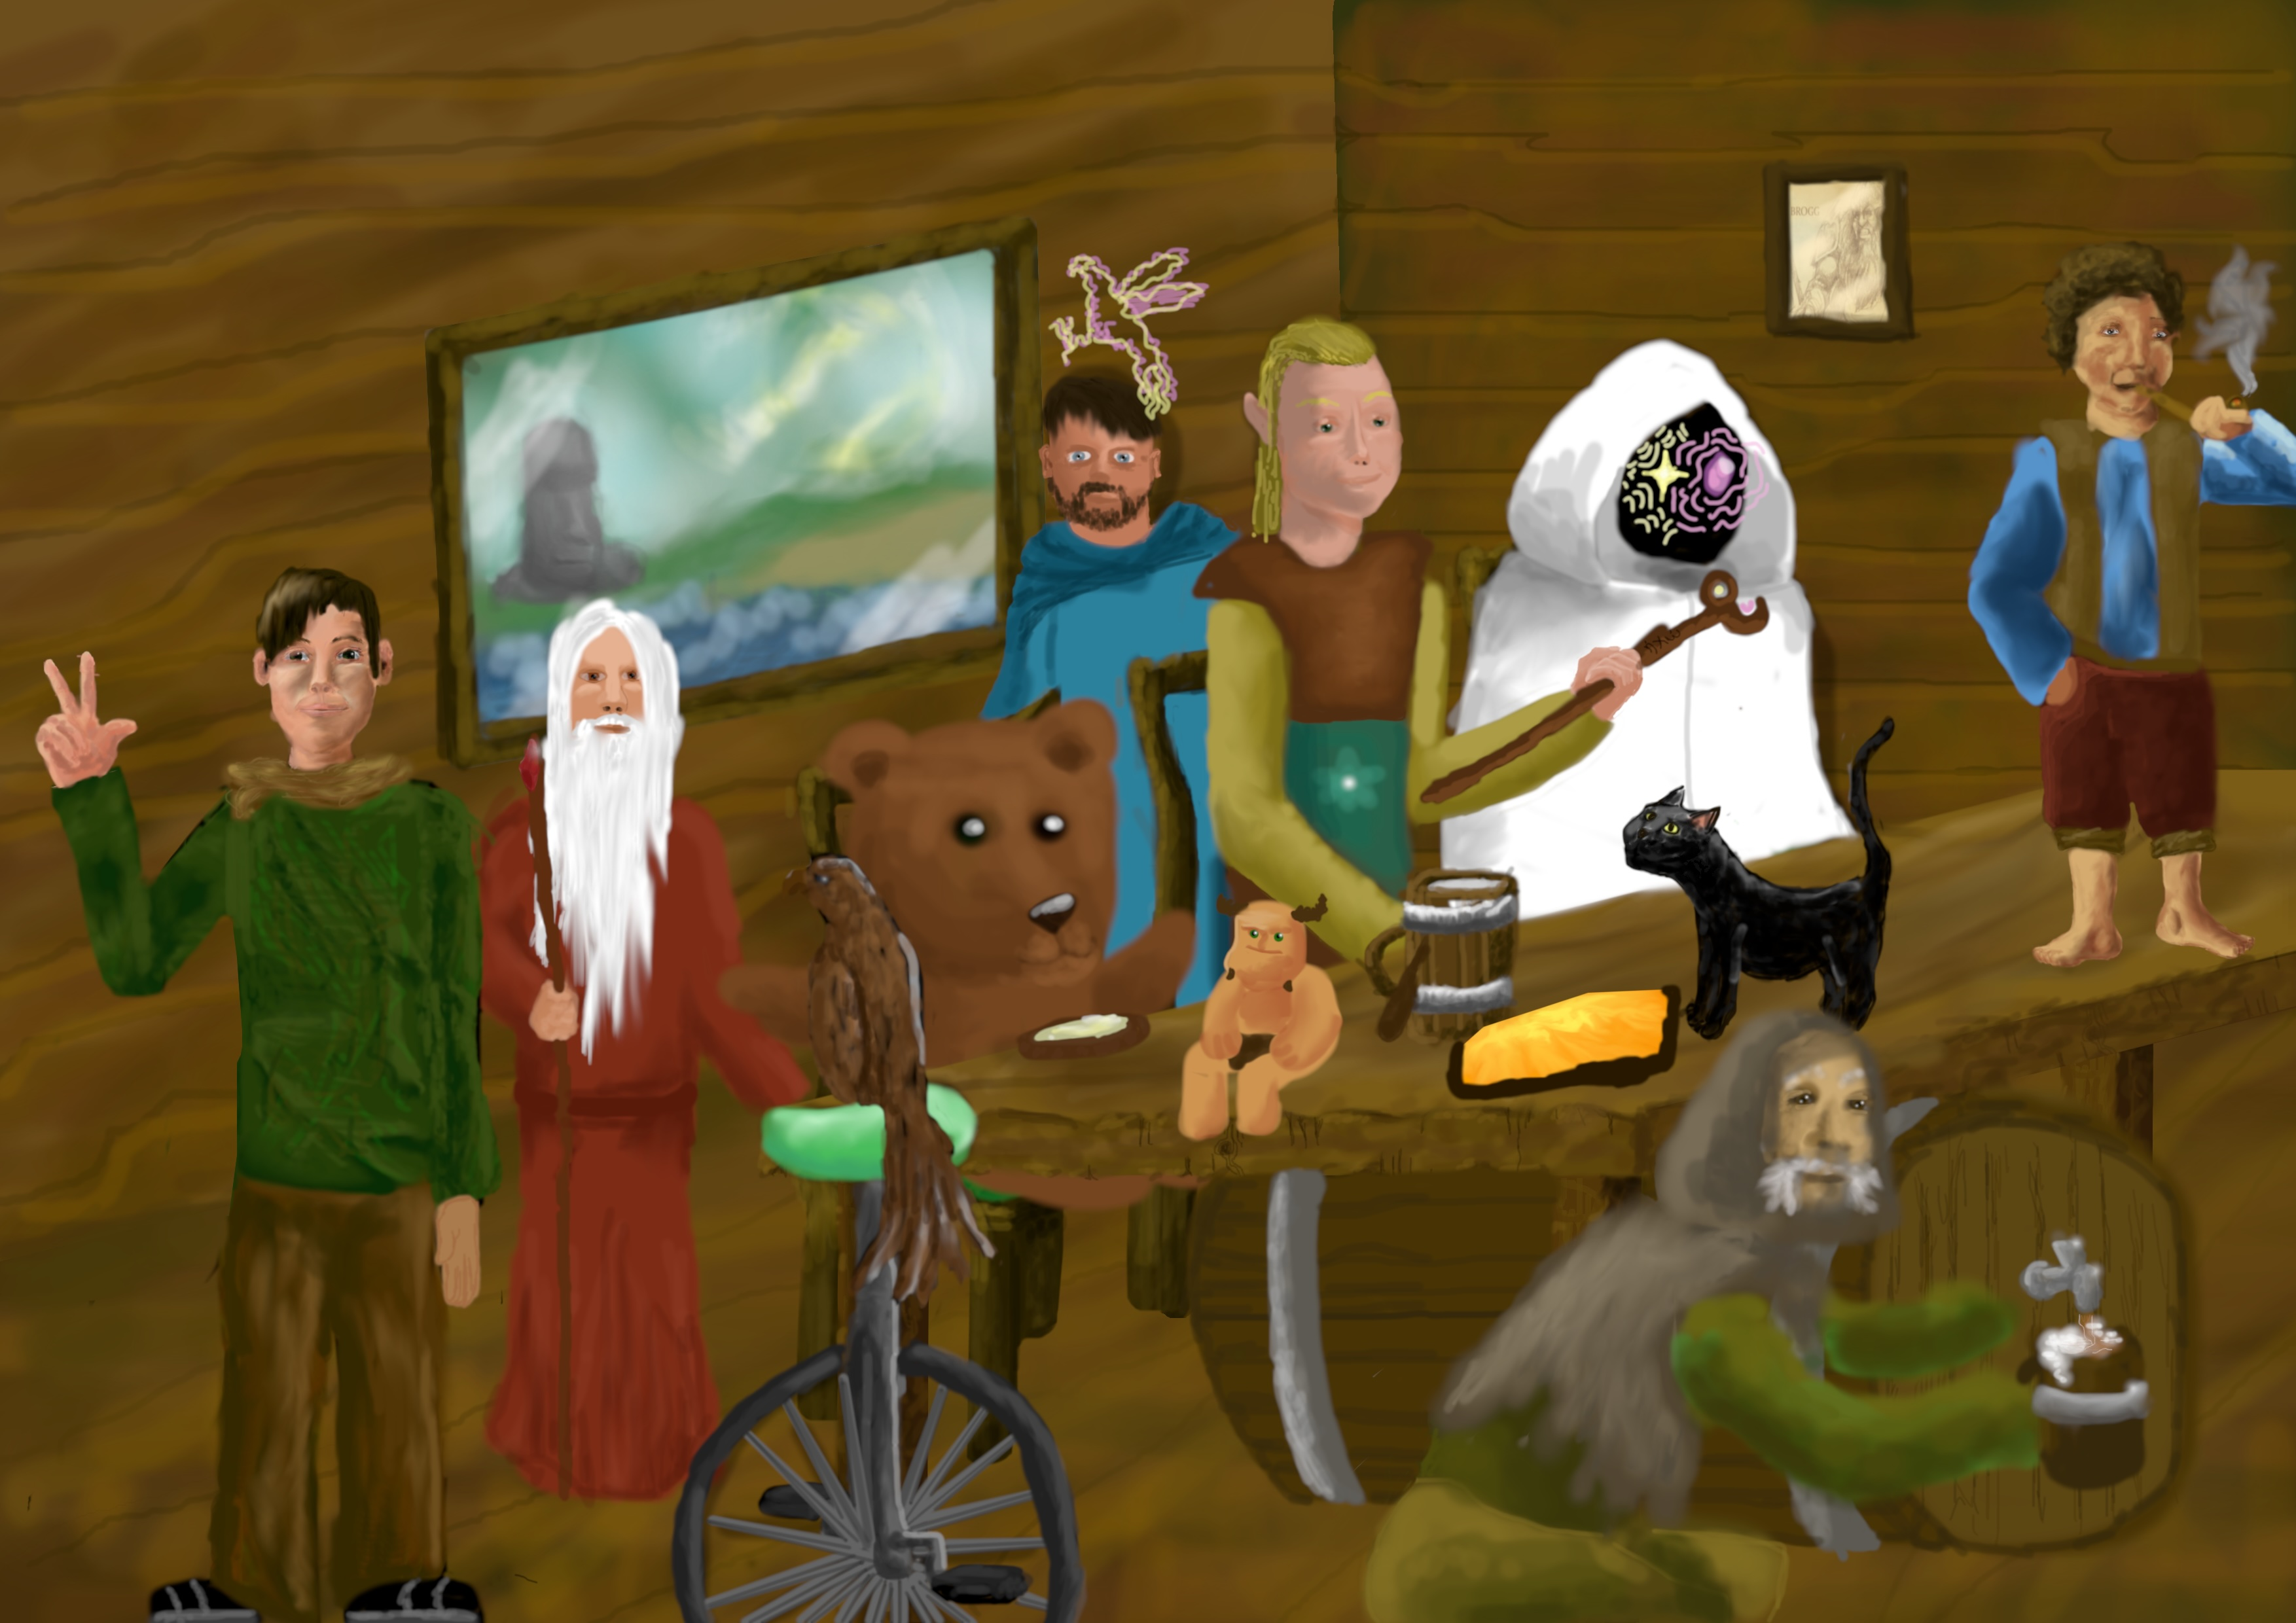
\includegraphics[height=120px]{Das Erbe des Wunderkindes/Bilder/Tavernenstammtischparty 2020 Gruppenbild.jpg}}\bigskip


In der Welt der bärig gebutterten Geschichtchen lebt, wie in der Sage des Butterbrotbären\footnote{Siehe \hypref{Stürmische Rätselnacht in der Taverne (2019 bis 2020)}} angetönt und in \hypref{Der Feuerkrieger und die Wassermagierin (2023)} konkretisiert, der Alchemist Naraven im Südlichen Wald. Er blickt mit seinem Hadrischen Spiegel tief in der Vergangenheit und hält seine Erkenntnisse auf danwarischen Steintafeln fest. Der Butterbrotbär dieser Welt ist eines der vielen Tiere, welche Naraven zu seiner magisch versteckten Hütte führen können – ebenjener Brummbär aus der Sage vom Butterbrotbären, welcher gerne Naravens Steintafeln stibitzt und gegen Gildas Butterbrote tauscht – aber die Taverne nicht betreten darf, weil Bären bekanntlich draußen bleiben. müssen\footnote{ Aus der Taverne, "Wie vertragen Dunkle Helden Gildas Met???":\\\includegraphics[height=120px]{Das Erbe des Wunderkindes/Bilder/Bären müssen draußen bleiben.jpg}}\bigskip



In der Welt von Frodos Mini-Erweiterung lebt ebenfalls ein Butterbrotbär im Südlichen Wald, dieser ist aber kleiner und weniger animalisch als derjenige aus der Sage. Er bietet ein beidseitig gebuttertes Bärenbrot an, welches einem Helden kurzzeitig Drukils Bärenstärke verleiht.\footnote{Aus der Taverne, "Minierweiterung: Die Tavernengäste": \textit{Ein kleiner brauner Bär stolperte aus dem Südlichen Wald und bot den Helden bereitwillig ein beidseitig gebuttertes Brot an.} 1x pro Legende kann ein Held, welcher an der Taverne (Feld 72) steht, das Bärenbrot verspeisen. Bis dieser Held seinen Tag beendet, hat er 3 Stärkepunkte mehr, dafür kann er solange keine Gegenstände, Gold, Edelsteine oder Holz tragen.}\bigskip


In der Welt der kollaborativen Fan-Geschichte "Das Abenteuer der Tavernengäste", die Albus der Bewahrer anstieß, kommt ein kleiner sprechender Bär vor, welcher allerlei Andor-Lore von sich gibt, gerne Butterbrote mampft und hier die Wunder magischer Waffeln kennenlernt.\footnote{Aus der Taverne, "Story: Das Abenteuer der Tavernengäste (Story)": [Butterbrotbär:] \textit{Die Tür schwang auf und eine gedrungene Gestalt stürzte in die Taverne hinein. Kleine Äuglein blinzelten unter einer beigen Kapuze hervor. Zwei Hände - oder war es Pfoten? - schoben sich aus Ärmeln hervor und wärmten sich am Feuer. Bibbernd streichelte die Gestalt die Tavernenkatze und fragte in die Runde: "Hat jemand ein Butterbrot? Ich komme gleich um vor Hunger!"} [Steppenechse111777:] \textit{Das Gegenüber von der Steppenechse war ein sonderbares Geschöpf: Es war ein kleiner Bär, in einen Umhang gehüllt, das besonderste Merkmal des Butterbrotbären war jedoch sein knurrender Magen. Er war in ganz Andor bekannt. Einmal als die Steppenechse zum ersten Mal die Taverne von Andor besucht hatte war sie ihm schon mal begegnet. Er hatte am Stammtisch gesessen und genüsslich ein Butterbrot gegessen.} [nic:] \textit{["]Hast du ein Butterbrot?" "Nein aber ein magisches Waffeleisen." antwortete Nic. "Äh...Was für eine magische Waffe?" fragte der Butterbrotbär verwirrt. "Ein magisches Waffeleisen. Damit presst man Teig zusammen und backt man ihn und schliesslich hat man eine sogennante Waffel" Er gab dem Bären das Waffeleisen und ein bisschen Teig.}} Nach eigener Aussage ist dies dieselbe Welt und derselbe Butterbrotbär wie damals, als Albus der Bewahrer zum ersten Mal Gildas (damals Garzes) gemütliches Gasthaus betrat.\footnote{Aus der Taverne, "Ein neuer Gast in der Taverne...": [Albus der Bewahrer:] \textit{Die Tür der Taverne schwang auf. Herein trat ein junger Bewahrer. "Bei Mutter Natur, ist das kalt da draußen!", beschwerte er sich. "Hallo, mein Name ist Albus.", stellte er sich anschließend vor, "Garz, ich hätte gerne eine warme Ziegenmilch!". Als er die Taverne betrat, sah er sich um. Etwas misstrauisch musterte er den Bären, der gerade ein Butterbrot verspeiste, oder den TroII, der gerade lebhaft, aber ruhig, mit einem anderen Gast diskutierte. Albus fühlte sich sofort wie zu Hause.} [Butterbrotbär:] \textit{Der Bär blickte schmatzend von seinem Butterbrot auf, um dem Neuankömmling fröhlich zuzuwinken. "Willkommen, holder Bewahrer Albus! Was für Neuigkeiten gibt es vom Baum der Lieder? Setze dich an den Kamin und genieße die Wärme – sofern die Schlafende Katze noch genug Platz davor gelassen hat. Wenn die Ewige Kälte noch viel länger anhält, werden wir bald von unserem hauseigenen Feuerdämon abhängig sein, um die Taverne gemütlich warm zu halten."}}\bigskip


In der Welt der kollaborativen Stammtischparty-Geschichte taucht in Kapitel 2 ganz kurz ein Butterbrotbär auf.\footnote{Aus der Taverne, "Kollaborative Geschichte Stammtischparty": [Schlafende Katze:] Im Laufe des Abends wohnten der Feier unter anderem Aoto, Galaphil, ein Schallmagier namens Liteus, ein Wesen, dass Hobbit genannt wurde, ein Elf aus den entfernten Elfenwäldern und ein andorischer Krieger mit dem Namen Piepe bei. Auch mehrere andere tierische Besucher gesellten sich zur Tavernenkatze: Der legendäre Butterbrotbär mit seinem Spielzeugtroll, für den Gilda extra das Bärenverbot der Taverne lockerte, ein danwarischer Phönix, den Trieest von dort mitgebracht hatte und ein andorischer Adler, der auf einem seltsamen Konstrukt, das wohl in Tulgor hergestellt worden war und sich "Einrad" nannte, saß. Sie alle saßen am schon fast legendären Tavernenstammtisch unter dem Bild eines tapferen Schildzwergs namens Brogg und einem Zauberfenster, durch das man eine sehr weit entfernte, sagenhafte Inselkette, auf der wohl von Mutter Natur persönlich erschaffen Steinstatuen standen, sehen konnte.} Wenn ich mich nicht irre, beschreibt diese Szene des Wachsamen Waldläufers Bild der Tavernengemeinschaft, welches weiter oben bereits genannt wurde.\bigskip

Der Tolle Troll, Barde der Kreaturen, führt ein Geschichtenbuch mit sich, auf dessen Cover\footnote{Aus der Taverne, "Bärig gebutterte Geschichtchen": [Butterbrotbär:] Ha! Ich habe in den Untiefen unserer Skype-Verläufe noch ein Original des Covers des Geschichtenbuchs des Tollen Trolls aufgespürt! :P\\ 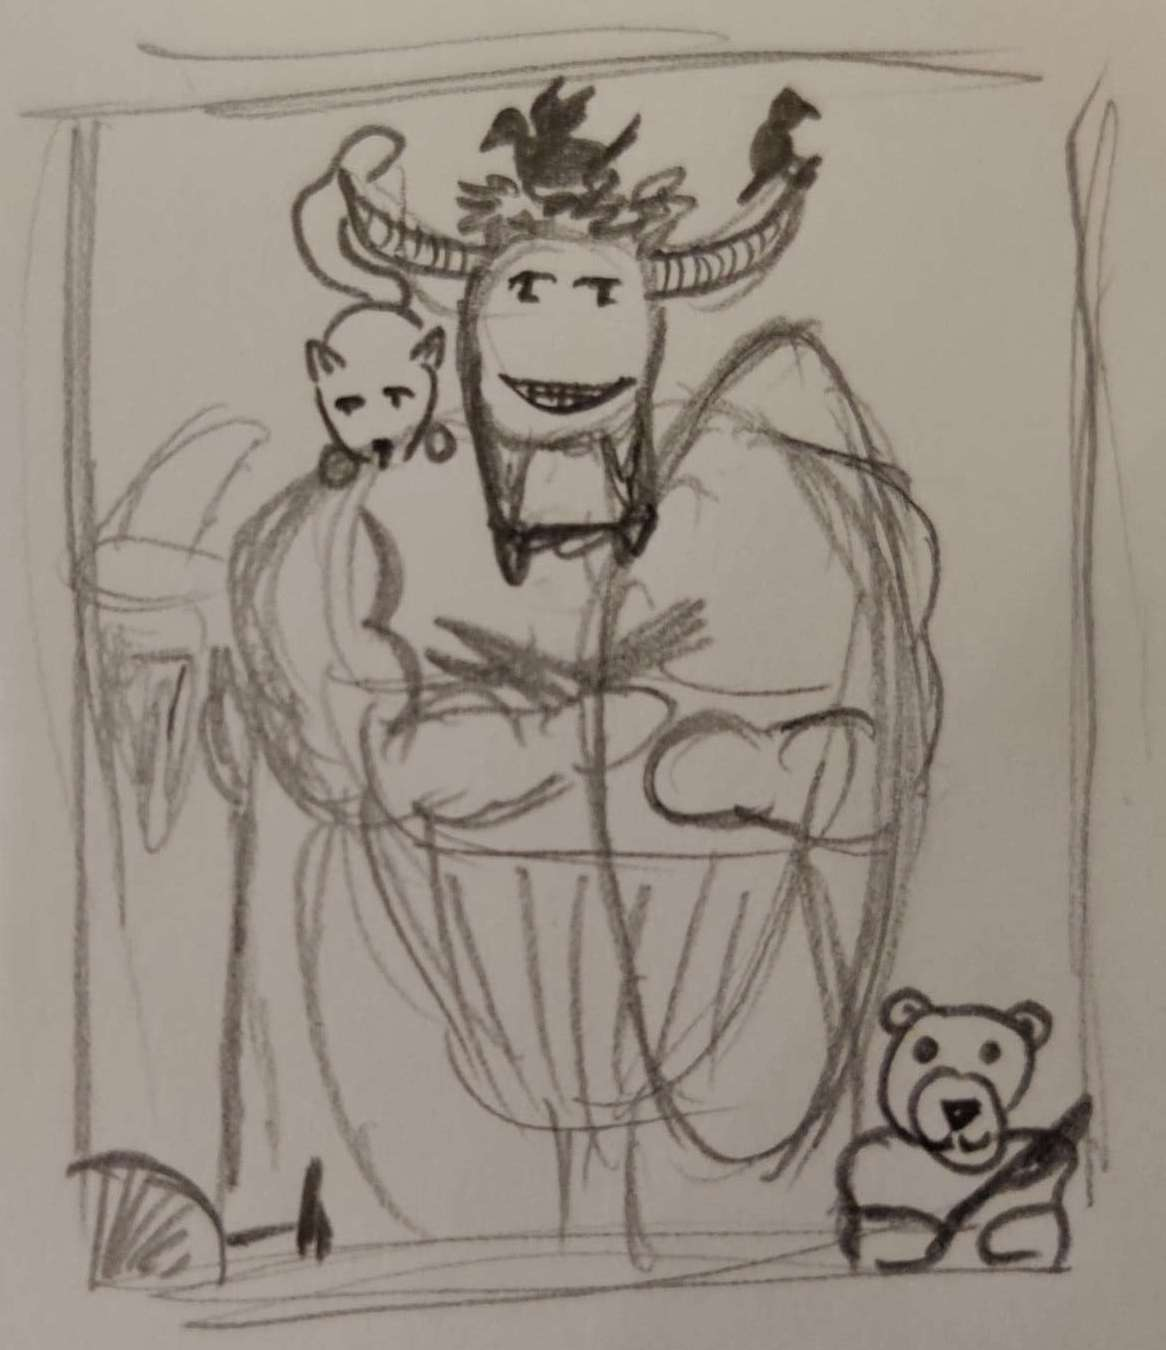
\includegraphics[height=120px]{Das Erbe des Wunderkindes/Bilder/Der Tolle Troll Geschichtenbuch Cover.jpg}} eine Skizze seiner selbst mit einigen Eastereggs ist. In der rechten unteren Ecke kann man einen weiteren Butterbrotbären erkennen, diesmal als Teddy mit toastförmigem Körper. So zeichnete ich den Butterbrotbären bereits in gemeinsamen Gartic-Phone-Partien.\bigskip

Natürlich gibt es in unserer Welt einen großen Andor-Fan, welcher unter dem Nicknamen Butterbrotbär auftritt, diesen Quark hier verfasst und schon so überhebliche Titel wie "Hüter der Andorchronik" zugesprochen bekam.\footnote{Aus der Taverne, "2020 – Neue Helden – Neue Legenden": [Bewahrer Melkart:] Ich werde dem obersten Hüter der Andorchronik nie mehr widersprechen :lol:} Towa zeichnete ihn in einem unglaublich coolen Jubiläums-Kreuzworträtsel,\footnote{Aus der Taverne, "26. Februar 2022: 3-Jahres-Jubiläum des Butterbrotbären": [Towa:] Jetzt sind es schon 3 Jahre, die der Butterbrotbär und ich in der Taverne sind! :D Herzlichen Glückwunsch zum Jubiläum, lieber Butterbrotbär! :mrgreen: Da darf natürlich ein Rätsel nicht fehlen. ;) Es sind lauter Begriffe aus der Andor-Welt versteckt, die gefunden werden müssen. Alle Richtungen sind möglich. Und alle Felder, die zu keinem Wort gehören, bilden ein passendes Bild. :P\\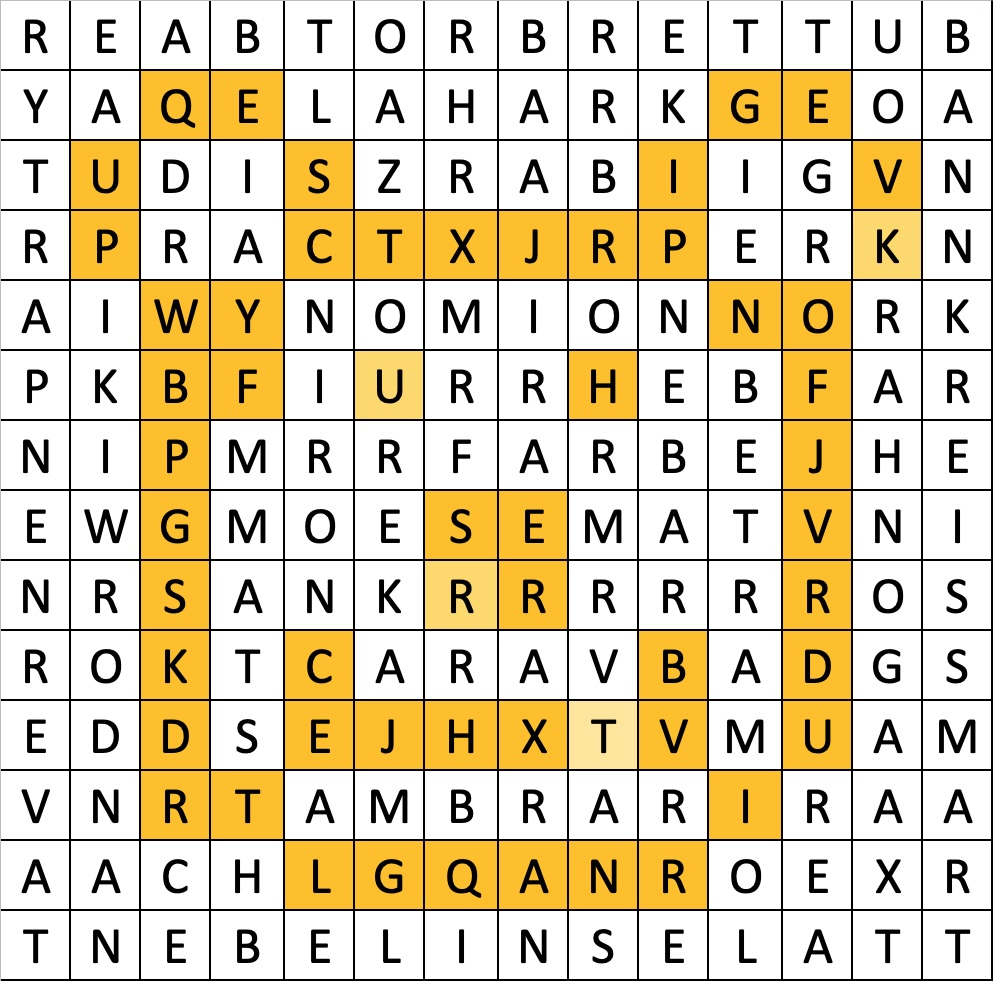
\includegraphics[height=120px]{Das Erbe des Wunderkindes/Bilder/Towa Raetsel BBB.jpg}} und Galaphil verfasste für ihn (als \textit{beste Beglückwünschungen bezüglich 2000 beachtlicher, belesener, beflissener, bedeutsamer, besonnener, beglückender, beispielloser, beredter und buchstäblich bemerkenswerter Beiträge in beige und braun},\footnote{Aus der Taverne, "Tavernentratsch": [TroII:] Bei Berthas bauchigem Bierfass! Ich bemerke, beinahe hätte ich Butterbrotbärs beeindruckende Beitragszahl bar jeder Beachtung belassen. :oops: Beste Beglückwünschungen bezüglich 2000 beachtlicher, belesener, beflissener, bedeutsamer, besonnener, beglückender, beispielloser, beredter und buchstäblich bemerkenswerter Beiträge in beige und braun! :P} habe ich mir sagen lassen :mrgreen:) sogar schon einen Fan-Helden.\footnote{Aus der Taverne, "Tavernentratsch": [Galaphil:] Butterbrotbär, Gelehrter von Andor, Rang 42, 1 Helm, 1 großer und 3 kleine Ablagefelder. 14 Stärke, 3 Zeilen Willenspunkte von 0 bis 20. Je ein Würfel pro Zeile. Sonderfähigkeit: bei der Aktion Laufen kann der Butterbrotbär immer ein Feld weiter laufen als er Stunden ausgibt. Bei der Aktion Kämpfen bekommt er pro Willenspunktzeile 1 Würfel extra, den er für selbst oder mitkämpfende Helden verwenden können. Im geeinsamen Kampf gilt: Jede/-r HeldIn darf dabei maximal einen Würfel bekommen. Kämpft er alleine, darf er natürlich alle Würfel selbst verwenden.}\bigskip

Und zu guter Letzt gibt es einen beigen Teddy, welcher sich bereits als digitaler Butterbrotbär in einen Sherwood Forest begab.\footnote{Vom Zuckerberg, "Robin Hood geht immer!":\\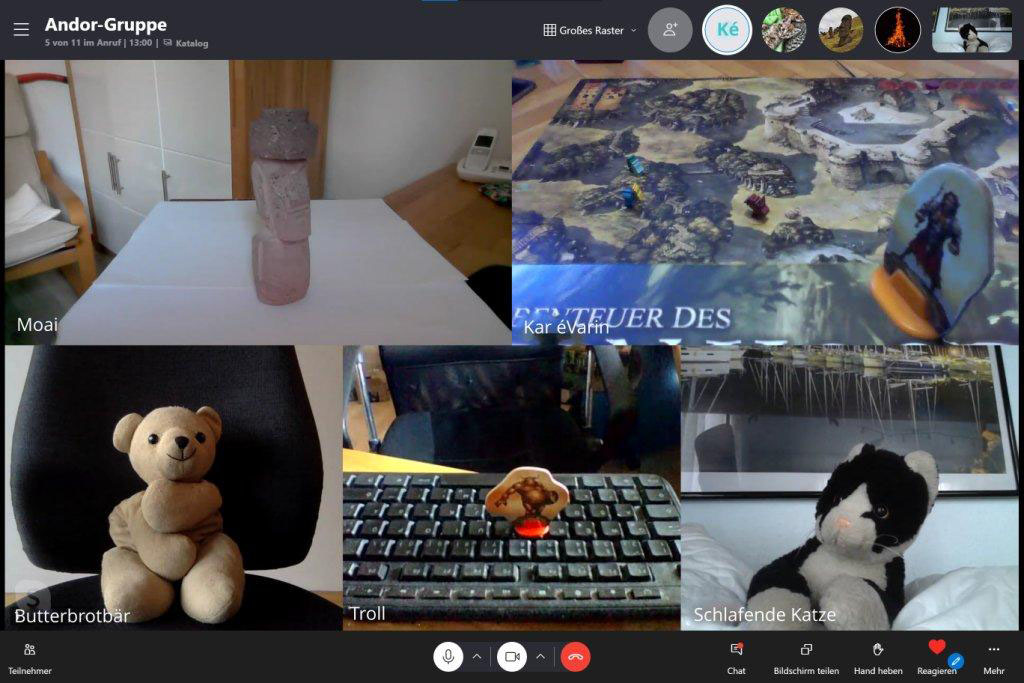
\includegraphics[height=120px]{Das Erbe des Wunderkindes/Bilder/Robin Hood geht immer!.jpeg}} Diesen Teddy kenne ich seit Geburt, und er sieht aktuell aus einem Regal zu, wie ich diese Worte schreibe. :D\bigskip


Tja, und wenn ich nichts übersehen habe, war es das auch schon – bislang. Wenn ich Leanders wäre, würde ich wohl voraussagen, dass Thorald eines Tages in einem Trunkenen Traum ... aber nein, diese Fan-Legende liegt noch in weit entfernter Zukunft. ;)

}


% TODO: Erwähne den Butterbrotbär in Thoralds Trunkenen Traum \url{https://legenden-von-andor.de/forum/viewtopic.php?f=5&t=10208}

% TODO: Erwähne mivos Botenbrief \url{https://legenden-von-andor.de/forum/viewtopic.php?f=11&t=4695&start=7439}

% TODO: Erwähne den Butterbrotbär im DfL-Begleitheft





%

\part{Weitere Werke}

\fancyhead[L]{\nouppercase{\lastrightmark}}



\begin{chapterbox}
    \chapter{Weitere wilde Werke eines Butterbrotbären}
    \label{Weitere wilde Werke eines Butterbrotbären}
    Andorische Fan-Werke meiner Wenigkeit, welche im Netz zu finden sind. Für eine vollständige Liste, siehe \url{https://legenden-von-andor.de/forum/viewtopic.php?p=116297\#p116297}.
\end{chapterbox}




{\parindent0pt



\az{diverse Jahre}

\section{Viel zu viele Fan-Held:innen (ab 2019)}

\begin{center}
    Fan-Held:innen aus der Taverne
\end{center}

\bildmitts[width=0.67\textwidth]{Heldencompilation.jpg}





\newpage


\section{Würfelerwartungswertberechnungen (ab 2019)}


\begin{center}
    Berechnungen aus der Taverne

    \url{https://legenden-von-andor.de/forum/viewtopic.php?p=110899#p110899}
\end{center}

\bildmitts[width=\textwidth]{Würfelerwartungswerte Icons.jpg}

\bildmitts[width=\textwidth]{Würfelerwartungswerte Zahlen.jpg}








\newpage
\section{Der Tolle Troll (2021)}

\begin{center}
    Fan-Held aus der Taverne

    \url{https://legenden-von-andor.de/forum/viewtopic.php?f=13&t=6119}
\end{center}

\bildmitts{Der Tolle Troll (2021).jpg}



\textbf{Ideen, Texte und Gestalltung:} Boggart, Butterbrotbär, Lost in the Echo und Schlafende Katze mit allerlei Impulsen vom Troll persönlich!\bigskip

Die Tavernengemeinschaft gratuliert dem ebenso rundum einzigartigen wie ideenreichen, Geschichten erzählenden, recht außergewöhnlichen Troll ganz herzlich zu 3000 Beiträgen hier im Forum!!!

Angesichts dieses außerordentlichen Anlasses konnten wir Anhänger der ausgezeichneten andorischen Allgemeinheit nicht davon absehen, als Anerkennung aller Aktivität und Arbeit dieses Auskenners einen frischen Fan-Helden anzufertigen.

Die Idee zur Willenspunkte-Vulnerabilität dieses Wesens haben wir womöglich von jemandem entwendet ;)

Im strahlend sonnigen Sommer, so sagt man, sieht man dieses sprachbegabte, selbstsichere Subjekt auf dem schönen Feld Sechs, sowohl beim souverän sarkastischen, schadenfrohen Scherzen als auch stundenlangem, sehr seriösen Schwafeln mit skeptischen, schreckhaft schüchternen, nach sicheren, schmalen Straßen suchenden Spaziergängern, beim schlauen Sinnieren über schlagfertige, stilbewusste Strategien sowie beim sinnlichen, schläfrigen Schnarchen im schattigen Schutz sanfter Sträucher.
Zur zwielichtigen, zeitweise zappendusteren (Winter-)Zeit zieht es diesen zuversichtlichen Zweibeiner zielstrebig zügig zum ziemlich zentralen Zugang einer Zwergenhöhle zurückliegender Zeiten, seinem zeitweilig zukünftigen Zuhause Feld Zwohundertneunzehn. Dort argumentiert er allabendlich mit allerlei anwesenden Argen in ausschweifenden Alliterationen über allgemeine Ausnahmen absurden Ausmaßes.

Karrenweise kommen kreuzende Kreaturen kurzum zu diesem Kenner kreativer Kurzgeschichten.
Viele Feinde finden völlig fälschlich Freude an Forns vielversprechend frohlockendem Freund.
Und wie bei Freund Forns Fähigkeit haben fesche Päsche fiese Folgen für freche Feinde.

\textbf{Dreitausend Dank an den tollen Troll im Namen aller Tavernengäste!!!}
\textbf{Die coole Creativ-Gaming-Force gegen chaotischen Covid-Frust.}

PS: Zu den lästigen Legenden der letzten Hoffnung liegen lauwarme Ideen vor.






\newpage
\section{Die Prinzessin von Andor (2021)}


\begin{center}
    Fan-Mini-Erweiterung aus der Taverne

    \url{https://legenden-von-andor.de/forum/viewtopic.php?f=8&t=6186}
\end{center}

\bildmitts{Die Prinzessin von Andor (2021).jpg}

\textbf{Erfinder:innen:} Boggart/Kar éVarin, Butterbrotbär,
Lost in the Echo, Schlafende Katze und Troll\bigskip

\textit{Es kam daher, vor langer Zeit,} \textit{ein Gast in die Taverne, ganz gescheit.}

\textit{Unbekannt waren Weg und Ziel,} \textit{wir wussten nur sein' Namen: Galaphil.}

\textit{In der Taverne, wohl bekannt,} \textit{leiht er stets eine helfende Hand.}

\textit{Und vor bald schon zwei Jahr',} \textit{brachte er die Idee des Stammtisches dar.}

\textit{Seitdem sind noch mehr bei Gilda zu Gast} \textit{und machen da mit Freuden Rast.}

\textit{Wir hoffen, es bleibt noch lange so,} \textit{und sind darüber äußerst froh.}

\textit{3000 Beiträge konntest du nun schon schreiben,} \textit{wir sind sicher, dabei wird es nicht bleiben.}

\textit{Und laut erschallt's in Andor noch,} \textit{der Galaphil, der lebe hoch!}








\newpage
\section{Kreaturenkarten statt Kreaturenplättchen (2023)}

\begin{center}
    Fan-Spielvariante aus der Taverne

    \url{https://legenden-von-andor.de/forum/viewtopic.php?f=8&t=9668}
\end{center}

\bildmitts{Kreaturenkarten (2023).jpg}
 

Wann immer ihr ein gewöhnliches Kreaturenplättchen ausführen würdet, zieht stattdessen zwei zufällige Kreaturenkarten und legt sie zufällig nebeneinander. Die beiden schwarzen Ziffern bestimmen das Zielfeld (falls dieses nicht existiert, wechselt die 10er-Stelle zur weißen Ziffer) und das einzige vollständige Symbol zwischen den beiden Karten gibt an, was auf dort erscheint (von links nach rechts). Danach werden die zwei Kreaturenkarten zurück in den Stapel gemischt.

Falls eine Kreatur durch Kreaturenkarten erscheinen sollte, aber es keine dieser Art mehr im Vorrat hat, erscheint stattdessen eine Kreatur der nächstschwächeren noch vorhandenen Art.

Falls eine Kreatur durch Kreaturenkarten auf ein Feld gestellt werden sollte, von dem kein Pfeil wegzeigt und/oder welches ein Kreaturen-Zielfeld ist (z.B. Rietburg, Lager der Tulgori oder Lager der Trolle), wird die Position dieser Kreatur stattdessen mit einem roten (10er-Stelle) und einem Heldenwürfel (1er-Stelle) ausgewürfelt, gegebenenfalls mehrfach.

Falls eine Kreatur durch Kreaturenkarten auf ein Feld gestellt wird, auf dem Bauern liegen, und von dem ein Pfeil wegzeigt, dürft ihr die Bauern auf das nächste kreaturenfreie Feld entlang der Pfeile versetzen.









\newpage
\section{ANDOR JUNIOR Erweiterungspaket (2020)}

\begin{center}
    Fan-Spielvariante aus der Taverne

    \url{https://legenden-von-andor.de/forum/viewtopic.php?f=8&t=5567}
\end{center}

\bildmitts{ANDOR JUNIOR Erweiterungspaket (2020).jpg}

\textbf{Erfinder:innen:} Schlafende Katze, Troll und Butterbrotbär

Kürzlich ist mir ein mysteriöses Paket per Falke zugestellt worden. Daran war ein Brief befestigt, welcher sich wie folgt anhört:

\textit{Dieses Andor-Junior-Fan-Erweiterungs-Paket besteht aus 11 Bonus-Helden, 9 Bonus-Aufgaben sowie einem Bonus-Endgegner.}

\textit{Die 11 Bonus-Helden sind Junior-Varianten der 11 noch nicht als Junior-Helden erschienenen offiziellen Helden (ausser Stinner). Jeder dieser Bonus-Helden ersetzt den offiziellen Junior-Helden seiner Würfelfarbe (bei Darh einer der drei). Prinzipiell könnt ihr aber auch mehrere Helden derselben Würfelfarbe gleichzeitig spielen, solange ihr im Voraus bestimmt, welcher Held welcher Heldenfarbe entspricht, wenn das für eine Aufgabe relevant sein sollte.}

\textit{Die 9 Bonus-Aufgaben können beliebig miteinander und mit den ursprünglichen Aufgaben gemischt werden. Sie benötigen oftmals Plättchen und Figuren aus dem Grundspiel oder einer Grundspiel-Erweiterung, diese können aber leicht ersetzt werden, falls ihr sie nicht besitzt.}

\textit{Mit dem neuen Endgegner könnt ihr euch nun endlich dem Drachen Tarok im Kampf stellen und die riesige Echse furchtlos vertreiben.}

\textit{Zu guter Letzt sei noch erwähnt, dass wir aus Gründen des Helden-Balancing empfehlen, bei der originalen Junior-Magierin gewürfelte Blitze als Fackeln zählen zu lassen.}

Spannend! Nur leider sieht es so aus, als hätte ein gewisser Schmierfink die Karten bereits vor mir in die Finger gekriegt und seine Meinung mit dunkler Tinte kundgetan.


\begin{center}
    Beiträge aus der Taverne

    "1. Tavernenstammtischparty!" (2020)
\end{center}

[Schlafende Katze:] Naja, eigentlich war ich ja schon die ganze Zeit da ;) Ich darf euch heute noch was zu Andor Ju...*\textbf{FAUCH!!!}*

[Varkur himself:] Muhahaha! :twisted: Seid gegrüßt, erbärmliches Gesindel! Habt ihr gedacht, ihr wäret mich los? Von Stund an werde ich sogar eure Kinder nicht mehr in Ruhe lassen! {\footnotesize Muhahahahaa! :twisted:}

[Towa:] Oh! Mit dem habe ich nicht gerechnet. Was willst du hier?

[Varkur himself:] Ich werde das Rietland brennen lassen! {\footnotesize Muhahahahaa! :twisted:}

[Tavernengaukler:] Der schon wieder... :x :o :lol:

[Varkur himself:] Schweig, Unwürdiger! Außer du willst um Gnade betteln. {\footnotesize Muhahahahaa! :twisted:}

[Lost In The Echo:] Varkur? Was hast du uns mitzuteilen? Sprich, bevor du aus diesem Ort des Friedens verstoßen wirst!

[Varkur himself:] Egal wer von euch sich mir in den Weg stellt, ob billiger Bettvorleger, wolfsvernarrter Wilder, würdelose Wasserplanscherin oder mickriger Möchtegernmensch: Ihr werdet scheitern! Ich kann es mit allen Helden aufnehmen! \textbf{ALLEN!} {\footnotesize Muhahahahaa! :twisted:}

Ich bin Varkur! Der mächtigste Dunkle Magier aller Zeiten! {\footnotesize Muhahahahaa! :twisted:}

Euch erwarten zahllose (neun) neue Herausforderungen: Torkelnde Trolle, aggressive Arbaks, fiese Fluggors... und meine Wenigkeit! Und selbst wenn ihr all das übersteht, wird es nicht mehr reichen, irgendwelche winselnden Welpen zu ihrer Mama zurückzuschleifen! Ihr werdet es mit Tarok persönlich aufnehmen müssen! :twisted: {\footnotesize Muhahahahaa! :twisted:}

[Lost In The Echo:] Da du ja scheinbar nicht an einer konstruktiven Unterhaltung interessiert bist, möchte ich in die Gruppe fragen, wer wohl mit dem billigen Bettvorleger gemeint ist : :?

[Varkur himself:] Der provisorische Pelzkragen natürlich... {\footnotesize Muhahahahaa! :twisted:}

[Schlafende Katze:] Was zu trinken? Oder doch lieber die Tür?

[Varkur himself:] Ein Rachenputzer … mit Olive. :) {\footnotesize Muhahahahaa! :twisted:}

[Schlafende Katze:] NARAVEN!!! Hast du noch was übrig von deinem Cocktail für unseren Gast?

[Boggart:] Einmal Thoraldmilch mit Olive, bitteschön! Wohl bekomms!

[Varkur himself:] Danke sehr. :P {\footnotesize Muhahahahaa! :twisted:}

[Varkur himself:] Ich habe schon genug Zeit in dieser verranzten Taverne verschwendet! Ich gehe wann ich will, nicht weil mich jemand vertreibt, das muss ich klarstellen. Aber ich werde wiederkommen! Ihr werdet gar nicht erst gegen den Drachen kämpfen, weil ihr davor an mir vorbeimüsst. An MIR!
Bis dann… {\footnotesize Muhahahahaa! :twisted:}

Muhahahaha! :twisted: *puff*

[Schlafende Katze:] Was ich eigentlich sagen wollte, bevor Varkur mich unterbrochen hat:

Der Troll, Butterbrotbär und ich haben uns ein bisschen mit Andor Junior beschäftigt.

Es sind \textbf{ALLE} offiziellen Helden jetzt spielbar und es gibt insgesamt neun neue Aufgaben.
Zusätzlich zu denen, die Varkur schon angedeutet hat gilt es Runensteine den Gors abzuluchsen, die Tulgori durch das Rietland zu begleiten und dem Trunkenen Troll unter die Arme zu greifen. Natürlich alles Kindgerecht!

Und als wäre das nicht genug, gibt es statt der Wolfssuche einen spannenden Drachenkampf am Schluss :)




\newpage
\az{Jahr 61}
\section{Arbon auf der Flucht (2021)}

\begin{center}
    Fan-Legende aus der Taverne

    \url{https://legenden-von-andor.de/forum/viewtopic.php?f=5&t=6396}
\end{center}

\bildmitts{Arbon auf der Flucht (2021).jpg}

\textbf{Erfinder:innen:} Butterbrotbär, Schlafende Katze, Troll

\textbf{Gestaltung:} Schlafende Katze

\textbf{Inhaltsangaben:} Diese Legende spielt nach dem Storytext „Die Geschichte des drittbesten Bogenschützen“ und vor dem Storytext „Die Hüterin und die Hexe“. Nachdem Arbon von Melkart, Pago und Folla in den Schwarzen Archiven überrascht wurde, befindet er sich nun auf der Flucht vor dem jungen Fährtenleser Fenn und den wütenden Bewahrern. In dieser Legende spielt einer der Mitspieler den Helden Arbon, der sich unsichtbar über das Spielfeld bewegt, während die Jäger sich auf die Suche nach ihm begeben. Dabei müssen sie den Verräter nicht nur finden, sondern auch zum Baum der Lieder zurück schleifen. Wenn nur die zusätzlichen Aufgaben und die vielen nervigen Gors nicht wären. Doch auch für Arbon ist die Flucht nicht leicht, denn scharfe Vogelaugen und die Jäger machen ihm das Leben schwer.

\textbf{Spielerzahl:} 2-4 Spieler

\textbf{Spielmaterial:} Grundspiel + Neue Helden

Erlebt ein unvergessliches (Schlafende-)Katz-und-Maus-Spiel quer durch Andor. Schwitzt mit Arbon, verzweifelt mit den Jägern und lasst euch nicht von unnötigen Storykarten irritieren!

\begin{center}
    Beiträge aus der Taverne

    "2. Tavernenstammtischparty 2021"
\end{center}

[Hogo:] für mich ein wasser, bitte. 
danke. mein gesicht ist sehr langweilig.

[Schlafende Katze:] Hogo, ein bisschen destruktiv eingestellt? Sooo hässlich bist du auch nicht :P

[Hogo:] hässlich ist auch nicht langweilig.

[Schlafende Katze:] mit Kapuze schwer zu beurteilen :P

[Hogo:] ja.

[Butterbrotbär:] Sind alle hier? Können wir loslegen? :D

[Hogo:] alle da! jetzt tür verriegeln und niemanden mehr reinlassen.

[...]

[AB von dem Andorwiki:] Hogo, beherrschst du die Handwerkkunst?

[Hogo:] nein. ich beherrsche gar nichts. beachtet mich nicht.

[Pago:] *In die Taverne stürz* Habt ihr ihn gesehen?
So einen jungen Barbar... Bisschen kleiner wie ich. Rote Haare. Rabe? Wenn, Denn, Venn... oder irgendwie so müsste er heißen. Ich hab eine Nachricht von ihm bekommen, dass er hier irgendwo wäre

[AB von dem Andorwiki:] Fenn?

[Pago:] Ja, genau so war der Name!!! Habt ihr ihn gesehen?

[Troll:] Nö, war schon seit 2016 (?) nicht mehr hier.

[Pago:] :shock: Das kann gar nicht sein! Ich habe ihn erst vor kurzem am Baum der Lieder getroffen, als er einen Auftrag angenommen hat.

[Butterbrotbär:] Wie kommst du denn darauf, dass Fenn hier wäre? Wollte er auch das Stammtisch-Jubiläum feiern?

[Pago:] Schön für euren Stammtisch. Dabei gibt es hier viel wichtigeres!!!

[Lost In The Echo:] Kannst du uns beschreiben, was er für Kleidung trug, als du ihn das letzte Mal gesehen hast?

[Pago:] Nunja. Keine Ahnung. Braun eben. Ist auch nicht so wichtig.... Wir hatten einige Schwierigkeiten am Baum der Lieder und Fenn sollte und bei der Suche nach einem verdächtigen Subjekt helfen
Ein mieser Verräter. Ehemals ein Wächter des Schwarzen Archivs. Hat Melkart mit einem Messer bedroht und ist dann abghauen. Arbon ist der Name dieses unwürdigen Stück Drecks...
Habt ihr wenigstens Kunde von IHM? Oder versteckt ihr ihn sogar in eurer Mitte?
*Durch die Taverne geh* *Besucher muster*

[AB von dem Andorwiki:] *zu Hogo schau* :?

[Hogo:] *sich ein bisschen in den schatten duck und leise die kekse mümmel

[Pago:] *vor dem Mann mit der schwarzen Kapuze stehen bleib, der Kekse mümmelt wie ein Kaninchen* *mit Bogen Kapuze aus seinem Gesicht streich* Wen haben wir denn hier? ARBON So sieht man sich wieder!

[Hogo:] abron? welch ein unvertraut klingender name. Ich bin hogo, ein einfacher knecht, dem der segen der bildung nicht zuteil wurde. ich kann auch nicht schreiben (außer das hier) und in den wachsamen wald habe ich zu lebzeiten noch keinen fuß gesetzt.
(und wenn ich doch dieser arbon wäre, wäre ich sicher nur hier, um mitzufeiern, und bestimmt nicht um in der menge der feiernden unterzutauchen)

[Pago:] Ach komm, erzähl keinen Stuss. Den kauft dir hier eh keiner ab! *Arbon am Schlaffitchen pack und vom Stuhl zerr*

[Hogo:] *dagegenzerr!!! ha! 6! das übertriffst du nicht! 8-)

[Pago:] Mist, eine 3...

[Hogo:] *schnell einen keks in den mund steck* sag ich doch! 8-)

[Pago:] *Arbon versuch noch eines ruterzuhauen* 4! du entkommst mir nicht! *Über Stuhl im Weg hechte*

[Hogo:] *bein stell

[Towa:] Arbon, brauchst du noch ein Heilkraut? Ich habe eines dabei!

[Hogo:] *wegrenn

[Pago:] *der Länge nach hinschlag* *Blut aus dem Gesicht wisch* *Schwer schnauf*

[Hogo:] kopf hoch, pago! (der ist so leicht, den kannst sogar du heben.) in anbetracht der schieren vielzahl deiner fehlschläge sind gewiss auch welche dabei, die nicht auf deine mangelden fähigkeiten zurückgehen :P *heldenfigur vom spielplan nehm

[Pago:] *Towa das Heilkraut abnehm* Ich danke

[Hogo:] Leise Stimme aus der Ferne: tut mir leid für die ziegenmilch und die gläser! pago bezahlt sicher gerne! tschühüss!

[Pago:] Verdammt, jetzt ist diese miese kleine Ratte schon wieder entwischt. Und von Fenns Raben keine Spur, wenn man mal einen Vogel braucht. So ein Mist! Dann muss ich wohl so nach ihm suchen. Vielleicht finde ich ja noch irgendwo Folla. *Hinter Arbon her aus der Taverne renn*
*umdreh und nochmal zur Türe reinschau* Wenn ihr mir doch noch helfen wollt, ihr wisst ja, wo ihr mich findet!!! [Link zu Arbon auf der Flucht] *Tür hinter sich zuschlag*

[Hogo:] *zum Fenster hereinschau* Wenn ihr mir helfen wollt übrigens auch. 8-)


\newpage
\az{Jahr 64}
\section{Flapsige Helden ins Land der Lagerfeuer (2023)}

\begin{center}
    Fan-Spielvarianten aus der Taverne

    \url{https://legenden-von-andor.de/forum/viewtopic.php?f=8&t=8615}
\end{center}

\bildmitts{Flapsige Helden ins Land der Lagerfeuer (2023).png}

\textbf{Alle Helden ins Land der Steppe}

Fan-Spielvariante, um mehr Helden, auch aus (annähernd) allen anderen Andor-Teilen, in DeK einzusetzen (nicht zwingend für die Einführungslegende geeignet).\bigskip

\textbf{Wächter der Lagerfeuer}

Fan-Mini-Erweiterung, um Helden aus DeK auch in (annähernd) allen anderen Andor-Legenden einzusetzen, oder einfach um mehr Variabilität ins Spiel zu bringen.
Einige Brunnen/Quellen kommen aus dem Spiel, dafür werden DeK-Feuerplättchen ins Spiel gebracht. Damit die Brunnen-Helden nicht traurig werden, könnt ihr auf die Feuer-Hausregeln aus "Alle Helden ins Land der Steppe" zurückgreifen.\bigskip

\textbf{Flapsig, fledrig und fuchsig}

Fan-Mini-Erweiterung, um Flaps Flederfuchs auch in anderen Andor-Teilen einzusetzen.




\newpage
\section{Zeit entzweit (2023)}

\begin{center}
    Fan-Legende zu "Die Kreaturen des Ava (2023)", aus der Taverne

    \url{https://legenden-von-andor.de/forum/viewtopic.php?f=25&t=9655}
\end{center}

\bildmitts{Zeit entzweit (2023).jpg}

\textbf{Erfinder:} Butterbrotbär

\textbf{Inhaltsangabe:} Instabile Zeitportale verbinden zwei Zeiten: Das herbstliche Andor, dessen Bewohner noch nichts von der ewigen Kälte ahnen, und das winterliche Andor, wo einige letzte Helden die Rietburg tapfer verteidigen. Ein mysteriöser Gegner ruft verschiedene Kreaturen des Ava herbei, die die Helden beschäftigen sollen. Doch nicht alle Kreaturen des Ava müssen im Kampf besiegt werden, denn sie wurden durch magische Banne in die Kontrolle des Gegners gebracht. Und es gibt diverse Möglichkeiten, solche Bänne zu brechen...

\textbf{Spielmaterial:} Grundspiel und "Die ewige Kälte", Andor-Spielpläne aus Grundspiel und "Die ewige Kälte"

\textbf{Schwierigkeitsgrad:} mittel bis schwer

\textbf{Chronologische Einordnung:} Während der vierten Legende aus Die ewige Kälte – unter anderem. ;)

\textbf{Heldenanzahl:} 2-4 getestet (empfohlen: 4 Helden), 5/6 theoretisch möglich

\textbf{Anmerkung:} Enthält signifikante SPOILER für Die ewige Kälte. Die Karten „Vorgeschichte“ und „Epilog“ enthalten ganz leichte Spoiler für „Düstere Zeiten“, können aber problemlos übersprungen werden.






\newpage
\az{Jahr 65}
\section{Legende 5 + Befreiung der Rietburg (2020)}

\begin{center}
    Fan-Spielkombination aus der Taverne

    \url{https://legenden-von-andor.de/forum/viewtopic.php?f=8&t=5295}
\end{center}

\bildmitts{Legende 5 + Befreiung der Rietburg (2020).jpg}

\textbf{Erfinder:} Boggart/Kar éVarin, unter Mitwirkung von Butterbrotbär, Galaphil, Schlafende Katze und Troll

\textbf{Inhaltsangabe:} Seit ich wusste, um was es in "Die Befreiung der Rietburg" geht, habe ich mich gefragt, ob sich das Spiel mit Legende 5: "Der Zorn des Drachen" kombinieren lässt. Vor euch liegt meine Antwort auf diese Frage!

Ab jetzt müssen die Kreaturen in der Rietburg nicht mehr mit Bögen bekämpft werden. Stattdessen können die Helden die Burg betreten und ihnen vor Ort den Garaus machen.
Der Schwierigkeitsgrad der Legende sollte sich dadurch nicht übermäßig ändern, maximal der Glücksfaktor wird noch etwas erhöht.



\newpage
\az{Jahr 66}
\section{Die verschwundene Krone (2021)}

\begin{center}
    Fan-Legende aus der Taverne

    \url{https://legenden-von-andor.de/forum/viewtopic.php?f=5&t=6445}
\end{center}

\bildmitts{Die verschwundene Krone (2021).jpg}

\textbf{Erfinder:} Butterbrotbär

\textbf{Inhaltsangabe:} Thoralds Krönung zum König von Andor kann nicht stattfinden, weil die Rietgraskrone verschwunden ist. Währenddessen geraten einige Tulgori im Grauen Gebirge in Schwierigkeiten.

\textbf{Chronologische Einordnung:} Frühjahr 66 a.Z.

\textbf{Benötigtes Material:} Grundspiel, Die Reise in den Norden und Die letzte Hoffnung.

\textbf{Spielpläne:} Graues Gebirge, Andor und Nebelinseln

\textbf{Schwierigkeitsgrad:} Schwer

\textbf{Heldenanzahl:} 2-4 getestet, 5/6 theoretisch möglich



\begin{center}
    Beiträge aus der Taverne

    "1. Tavernenstammtischparty!" (2020)
\end{center}

\bildmitts{Die verschwundene Krone Ankündigung Bild 1.jpeg}

Ihr habt ja bestimmt auch schon die Gerüchte gehört, dass die Helden von Andor einst eine ereignisreiche Epoche erlebt hätten, in welcher manche von ihnen auf der Aldebaran ins Hadrische Meer stachen, während andere zur selben Zeit Meilen entfernt durchs Graue Gebirge stapften. Doch eine solche Legende wurde zumindest hier in der Taverne noch nicht erzählt...

So suchte ich eines gemütlichen Abends hier in ebendiesem Schankraum die Gesellschaft von Fenn dem Fährtenleser und fragte ihn, ob an jenen Gerüchten etwas Wahres dran sei.

\bildmitts{Die verschwundene Krone Ankündigung Bild 2.jpeg}

Fenn ist begnadeter Geschichtenerzähler, und so dauerte es nicht lange, bis er begeistert eine Erzählung zum Besten gab, von einer Zeit, als Prinz Thorald eigentlich zum König von Andor gekrönt hätte werden sollen, als gleich zwei unerwartete Angelegenheiten dazwischen kamen, welche die Helden in entgegengesetzte Himmelsrichtungen schickten...

Zurück in meiner gemütlichen Hütte versuchte ich bei einer dampfenden Tasse kostbaren Schokogebräus, das Gehörte, so gut ich konnte, zu Pergament zu bringen.

\bildmitts{Die verschwundene Krone Ankündigung Bild 3.jpeg}

Laut Fenns Bericht waren einige Helden vor Sidra, der Küste Andors, an Bord der Aldebaran gegangen... doch als ich dies mit einigen alten Karten Andors abglich, war vor Sidra gar kein Anlegeplatz eingezeichnet! Kurzerhand musste ich mir einen hinzudichten. Ähnlich erging es mir bei der Suche nach einem durchgehenden Weg ins Graue Gebirge. Und an manchen Stellen könnte Fenn im Erzählfieber die Wahrheit etwas ausgeschmückt haben... ein waschechter Arrog am Baum der Lieder?!

Kleine Hindernisse waren etwa meine Unerfahrenheit in der Kunst des Legendenschreibens oder auch mein Stubentiger, der in all meinen Notizen immer bloss Schlafgelegenheiten sah. :P

\bildmitts{Die verschwundene Krone Ankündigung Bild 4.jpeg}

Zum Glück konnte ich auf die umfangreiche Unterstützung anderer Andori zählen!
Nun hoffe ich, diese verworrene Geschichte bald hier vorstellen zu können – und dass sie vielleicht andere Tavernengäste dazu anregt, weitere Berichte dieser Sorte zusammenzutragen.




\newpage
\az{Jahr 71}
\section{Krankheit in Cavern (2022)}

\begin{center}
    Fan-Legende aus der Taverne

    \url{https://legenden-von-andor.de/forum/viewtopic.php?f=5&t=7093}
\end{center}

\bildmitts{Krankheit in Cavern (2022).jpg}


\textbf{Erfinder:} Butterbrotbär

\textbf{Inhaltsangabe:} Unsere Helden wollen kranke Zwerge in der Schatzkammer Caverns versammeln, auf dass diese dort geheilt werden können. Wenn ihnen nur nicht all dieses Geröll und all diese Kreaturen den Weg versperrten …

\textbf{Benötigtes Material:} Grundspiel, Alte Geister („Feld 37“-Überleger, eine zufällige Quelle, „Baum der Lieder“-Plättchen und Hallgard) und Düstere Zeiten („Feld 83“-Überleger, Mart und Kjall).

\textbf{Benötigte Vorkenntnisse:} Minen-Regeln aus Legende 4 und Gift-Regeln aus Legende 5.

\textbf{Heldenanzahl:} 2-4 getestet, 5/6 theoretisch möglich

\textbf{Chronologische Einordnung:} Ende 71 a.Z.

\textbf{Schwierigkeitsgrad:} Leicht

\textbf{Spielplan:} Cavern



\newpage
\az{Jahr 74}
\section{Der sagenumstohlene Eismet (2021)}

\begin{center}
    Fan-Abenteuer aus der Taverne

    \url{https://legenden-von-andor.de/forum/viewtopic.php?f=8&t=6658}
\end{center}

\bildmitts{Der sagenumstohlene Eismet (2021).jpg}


\textbf{Erfinder:} Butterbrotbär

\textbf{Inhaltsangabe:} Das einst vom mächtigsten Magier Orweyn über den Eingang des Eisernen Turms gelegte Siegel war schon vor langer Zeit vom jungen Magier Varkur gesprengt worden. Doch das hinderte die Zauberer des Turms nicht daran, die darin eingeschlossenen Geheimnisse wacker zu wahren. Bis jetzt.

In späteren Jahren sollten sich Chronisten darüber uneinig sein, wann genau die Tore zum Eisernen Turm geöffnet wurden. Drangen Zauberer des Feuers mithilfe der Helden von Andor in sein Inneres, um die legendären Magischen Waffen zu erringen? Brach der Trunkene Troll auf der Suche nach dem sagenumwobenen Eismet aus der Vergangenheit Hadrias in das geschichtsträchtige Gemäuer ein? Fest steht, dass der Eisernen Turm in diesen chaotischen Zeiten kurzzeitig nicht mehr gesichert wurde.

So gelang es einem diebischen und außergewöhnlich willensstarken Nerax, ein wertvolles Pergament aus dem jahrhundertelang verschlossen gebliebenen Turm zu erringen. War dies etwa das Geheimrezept für den sagenumwobenen Eismet, von dem Braumeister Borabil einst dem wackeren Andori Erloth berichtet hatte?

Earas Aufgabe: Überwinde den diebischen Nerax und nimm das gestohlene Pergament wieder an dich!


\textbf{Benötigtes Material:} Modifizierte "Adventures of Hadria"-Datei.

\textbf{Spielplan:} Feste von Yra

\textbf{Schwierigkeitsgrad:} Sehr leicht

\textbf{Heldenanzahl:} 1 (Eara)






\newpage
\az{Jahr 75}
\section{Alle Helden ins Graue Gebirge! (2019)}

\begin{center}
    Fan-Spielvariante aus der Taverne

    \url{https://legenden-von-andor.de/forum/viewtopic.php?f=8&t=4871}
\end{center}


\bildmitts{Alle Helden ins Graue Gebirge! (2019).jpg}

\textbf{Erfinder:} Butterbrotbär

\textbf{Inhaltsangabe:} Mit dieser Spielvariante sollte man alle offiziellen Helden des Grundspielplans und viele Fan-Helden jetzt auch in Andor Teil III spielen können.

Diese Karten hier können nicht und sollen auch nicht die auf einzelne Helden, deren SF und deren Charakterentwicklung abgestimmten Helden-, Erschöpfungs- und Hoffnungskarten ersetzen. Vielmehr ging es mir darum, möglichst allgemeine Helden-, Erschöpfungs- und Hoffnungskarten zu erstellen, damit man auch in der letzten Hoffnung eine möglichst offene Heldenwahl hat.

Praktisch ist, dass man die allgemeinen Karten aus dieser Spielvariante problemlos mit spezifischen Karten mixen kann: Falls jemandem beispielsweise eine gute zweite Sonderfähigkeit für Orfen einfällt, kann er diese selbstverständlich benutzen – und für alle noch fehlenden Karten (z.B. Geschenkaufgaben und Erschöpfungskarten) einfach auf Karten aus dieser Fan-Erweiterung zurückgreifen.






\newpage
\az{Jahr 76}
\section{Renn, Forn, renn! (2022)}

\begin{center}
    Fan-Legende aus der Taverne

    \url{https://legenden-von-andor.de/forum/viewtopic.php?f=5&t=7893}
\end{center}

\bildmitts{Renn, Forn, renn! (2022).jpg}

\textbf{Erfinder:} Butterbrotbär


\textbf{Inhaltsangabe:} Eine Horde gepanzerter Trolle trottet nach der Befreiung der Winterburg auf den ungeschützten Tross der Andori zu. Forn, der scheue Schattenskral, ist stark und schnell, doch auch weit weg. Wird der Halbskral noch rechtzeitig zur Rettung heranrasen können? Manch ein anderer Dunkler Held wird ihn auf seinem Weg unterstützen – oder selbst Unterstützung benötigen.

\textbf{Benötigtes Material:} Die letzte Hoffnung \& Dunkle Helden

\textbf{Chronologische Einordnung:} 76 a.Z., nach Legende 16

\textbf{Schwierigkeitsgrad:} Leicht

\textbf{Spielplan:} Graues Gebirge

\textbf{Heldenanzahl:} 1 (Forn)





}










\begin{chapterbox}
    \chapter{Weitere wunderbare Werke der Andor-Fan-Community}
    \label{Weitere wunderbare Werke der Andor-Fan-Community}
    Einige außergewöhnliche andorische Fan-Werke, welche im Netz zu finden sind. 
\end{chapterbox}

\extramarks{}{}

{\parindent0pt

\section{Die Taverne in Aufruhr (2014)}

\begin{center}
    Fan-Legende aus der Taverne

    \url{https://legenden-von-andor.de/forum/viewtopic.php?f=5&t=943}
\end{center}


\bildmitts{Gildas Bild der Woche Das brachte der Osterhase! (2015).jpg}


\textbf{Fan-Legenden-Erfinder:} Diese Legende wurde zwischen Mai und September 2014 von den Mitgliedern des offiziellen Forums “Die Taverne von Andor” entwickelt.

\textbf{Inhaltsangabe:} Vor langer Zeit hatte Erloth aus den Überresten eines zerstörten Karrens einen Marktstand errichtet, verkaufte Met und Wein, und bald war daraus eine kleine Hütte geworden - “Die Taverne zum Trunkenen Troll”. Händler, Reisende und Helden gingen ein und aus, und die Wirtin Gilda, Erloths Enkelin, war im ganzen Land bekannt und beliebt. Oft genug waren Kreaturen durch Andor gezogen, doch nie hatte eine von ihnen gewagt, die Taverne anzugreifen, und kein Mensch hatte das jemals für möglich gehalten. Bis zu jenem Morgen, als ein Bauer die Helden erreichte und rief: “Kommt schnell! Der Trunkene Troll verwüstet die Taverne!”

\textbf{Schwierigkeitsgrad:} mittel

\textbf{Spieleranzahl:} Die Legende kann mit 2-6 Helden gespielt werden.

\textbf{Info:}
Die Legende spielt auf der Vorderseite des Grundspiel-Plans. Es werden die Sternenschild-Erweiterung und die Ergänzung "Neue Helden" benötigt.









\newpage
\section{Der sagenumwobene Eismet (2016)}

\begin{center}
    Fan-Legende aus der Taverne

    \url{https://legenden-von-andor.de/forum/viewtopic.php?f=5&t=2744}
\end{center}



\bildmitts{Der sagenumwobene Eismet (2016).jpg}


\textbf{Fan-Legende:} Der sagenumwobene Eismet
\textbf{2. Fan-Legende der Tavernengemeinschaft}

\textbf{Fan-Legenden-Erfinder:} Diese Legende wurde zwischen Mai 2015 und August 2016 von den Mitgliedern des offiziellen Forums “Die Taverne von Andor” entwickelt.

\textbf{Inhaltsangabe:} Qurun war besiegt! Doch seine letzten Worte hallten den Helden in den Ohren nach. `Andor brennt und ihr seid weit weg...´ hatte er ihnen noch im Sterben höhnisch ins Gesicht geschleudert. Die Helden verloren keine Zeit und brachen sofort auf. `Wir müssen zurück nach Andor!´Doch als sie endlich den Steg erreichten, wo die Aldebaran vor Anker lag, sahen sie mit Entsetzen, dass der Mast gebrochen und das Segel zerfetzt war...

\textbf{Schwierigkeitsgrad:} variabel, von leicht bis sehr schwer

\textbf{Spieleranzahl:} Die Legende kann mit 2-6 Helden gespielt werden.

\textbf{Info:}
Die Legende spielt auf der Rückseite des Nord-Spielplans (Hadria). Es werden neben dem Grundspiel die Erweiterungen „Die Reise in den Norden“, „Der Sternenschild“ und „Neue Helden“ benötigt.
Die Legende schließt inhaltlich direkt an die Geschehnisse der Legende 10 an. Bei der Entwicklung der Legende wurde ein ganz besonderes Augenmerk auf den erzählerischen Aspekt gelegt.

\textbf{Spieldauer:} min. 2 Stunden








\newpage
\section{Das Lied des Königs – Die Neuen Helden (2019)}

\begin{center}
    Fan-Legende aus der Taverne

    \url{https://legenden-von-andor.de/forum/viewtopic.php?f=5&t=4817}
\end{center}

\bildmitts{Gildas Bild der Woche Legendäre Freuden (2019).jpg}


\textbf{Fan-Legenden-Erfinder:}
Entstanden als Gemeinschaftsprojekt in der Taverne: Projekt: Das Lied des Königs

\textbf{Inhaltsangabe:}
Derzeit erreichen uns Berichte, wie die Neuen Helden nach Andor kamen. Auch wir stießen auf solche Geschichten, doch berichten unsere Quellen von ganz anderen Geschehnissen.
Lasst Euch erzählen, was wir über Arbon, Bragor, Fenn, Kheela, Orfen und Forn zur Zeit der Anfänge der Helden von Andor hörten!

\textbf{Schwierigkeitsgrad:}
mittel bis schwer, abhängig von Helden- und Endgegnerwahl

\textbf{Spielerzahl:} 1-6 Helden

\textbf{Info:}
Die Legende spielt auf dem Andor-Spielplan. Neben dem Grundspiel werden die Erweiterungen "Der Sternenschild" und "Die BonusBox", die Feinde von Andor sowie, je nach Heldenwahl, die Merhspielererweiterungen "Neue Helden" und "Dunkle Helden" benötigt.
Die Legende spielt parallel zum Roman "Das Lied des Königs" und nimmt gelegentlich Bezug auf dessen Handlung. Die Kenntnis des Romans wird nicht vorausgesetzt, doch können wir jedem, der ihn noch nicht gelesen hat, dies nur empfehlen!

\textbf{Spieldauer:}
Abhängig von der Heldenwahl, da jeder Held seine eigenen Aufgaben mit sich bringt.





\newpage
\section{Ära der Händler (2014)}

\begin{center}
    Fan-Erweiterung aus der Taverne

    \url{https://legenden-von-andor.de/forum/viewtopic.php?f=8&t=1162}
\end{center}

\bildmitts{Ära der Händler Tafeln.jpg}

548 Beiträge, 59 Seiten, 5 Threads und etwas mehr als 2 Monate hat es gedauert bis wir euch eine (fast) fertige Version der großen Gegenstandserweiterung - \textbf{Ära der Händler} heute vorstellen können. Auf \textbf{5} neuen Händlertableaus findet ihr über \textbf{30} neue Gegenstände mit einzigartigen Funktionen, die nur darauf warten von euren Helden, im Kampf gegen das Böse, eingesetzt zu werden. Ich wünsche euch viel Spaß und Würfelglück ;)!

Ein großer Dank an \textbf{alle} Beteiligten die stets getestet, hinterfragt und die nötigen Ideen geliefert haben, ohne dies wäre diese Erweiterung nie so toll geworden!
Ganz besonders möchte ich mich bei Garz der Händler, Fussssohle, Speerkämpfer, Ent, Tost, RoninBubu, Mjölnir und Karl Schlag bedanken, die viel Zeit in die Entwicklung gesteckt haben.



\newpage
\section{Tulgorische Abenteuer (2020)}

\begin{center}
    Fan-Legenden aus der Taverne
\end{center}

\bildmitts{Tulgorische Abenteuer (2020).jpg}



\begin{center}
    "Wüstenabenteuer: Der Merasteintransport"

    \url{https://legenden-von-andor.de/forum/viewtopic.php?f=5&t=5370}
\end{center}

\textbf{Fan-Legenden-Erfinder:} Falkenstadl

\textbf{Einleitung}
Die Zeiten nach den vielen Kämpfen in Andor waren von Hoffnung erfüllt. Hoffnung auf einen Frieden, der es allen erlaubte in Sicherheit mit ihren Familien zu leben und zu arbeiten. Die Arbeit war schwer, ja – aber sie war erfüllend und ernährte die ganze Sippschaft.
Nach getaner Arbeit konnte man sich auch wieder gefahrlos in der Umgebung bewegen um die Taverne zu besuchen. Sie war nicht nur eine Zuflucht in Notzeiten, sondern auch stets der Ort zum Austausch der interessentesten Neuigkeiten. So kam es an einem Abend im „Trunkenen Troll“ zu einem Treffen unserer Helden von Andor. Man gönnte sich ein gut gefülltes Horn und sprach über allerlei Belangloses und über Heldentaten, aber auch über so manchen traurigen Verlust.




\begin{center}
    "Wüstenlegende: Verschollene Freunde"

    \url{https://legenden-von-andor.de/forum/viewtopic.php?f=5&t=5590}
\end{center}

\textbf{Fan-Legenden-Erfinder:} Phoenixpower


\textbf{Inhaltsangabe:} Bei der Überquerung des Fahlen Gebirges wurden Thorn, Kram und Marek, der Sohn Merriks von Chada und Eara getrennt. Nun versuchen Thorn und Kram gemeinsam mit ihren neuen Freunden Tugor und Tugira die beiden wiederzufinden.

\textbf{Schwierigkeitsgrad}: Variabel
Je weniger Helden mitspielen, desto leichter ist die Legende, zudem könnt ihr die von Falkenstadl beschriebene „\textit{Wünsch dir was-Methode}“ nutzen.

\textbf{Benötigtes Material:} Grundspiel, das Wüstenabenteuer von Falkenstadl, diese Legende





\begin{center}
    "Abenteuer in Tulgor: Der Spruch des Gepodon"

    \url{https://legenden-von-andor.de/forum/viewtopic.php?f=5&t=5851}
\end{center}


\textbf{Fan-Legenden-Erfinderin:} Flederfluse

\textbf{Legendenziel:} Beschützt die Erträge der tulgorischen Feldwirtschaft. Das Getreide, die Schafe, die Hühner und die Obstbäume.

Verhindert, dass die Kreaturen auf ihre Zielfelder gelangen. Sobald eine Kreatur ihr zweites Zielfeld erreicht hat, kommt sie auf eines der beiden „Goldenen Schilde“. Es dürfen nur zwei verschiedene Kreaturen auf die Schilde.
Sobald eine dritte Kreatur, oder eine zweite Kreatur der gleichen Art ihr zweites Zielfeld erreicht, ist die Legende verloren.




\newpage
\section{Die Odyssee (2021)}

\begin{center}
    Fan-Legende aus der Taverne

    \url{https://legenden-von-andor.de/forum/viewtopic.php?f=5&t=6037}
\end{center}


\bildmitts{Die Odyssee (2021).jpg}

\textbf{Fan-Legenden-Erfinder:} Vakmar \& Vakur
\textbf{Audio-Dateien: }Cassia u. Vakur

\textbf{Kurzbeschreibung:} Die Helden erleben eine Irrfahrt im Hadrischen Meer.

\textbf{Informationen:} Die Legende ist an Homers Odyssee angelehnt; ansonsten ist sie frei erfunden und spielt nicht vor, zwischen, während oder nach den offiziellen Legenden.
\textit{Hinweis:} Die Spielvariante „Grenolin“ und die Heldenfigur Stiana können in dieser Legende nicht genutzt werden.

\textbf{Erfahrung:} L10; Im Dienste des Feuers (Die Handhabung der Magischen Waffen sollte bekannt sein.)

\textbf{Material:} Die Legende spielt auf der Vorderseite der Erweiterung „Die Reise in den Norden“ (Nebelinseln).
Neben dem Grundspiel wird noch die Erweiterung „Die Reise in den Norden“ benötigt.
Auf der letzten Seite gibt es einen „Bastelbogen“. Dieser enthält Material, das ebenfalls benötigt wird; alternativ kann aber auch anderes Spielmaterial verwendet werden.
Die Seeschlange ist der sehr zu empfehlenden Fan-Legende „Das Juwel der Mächte“ entnommen.

\textbf{Schwierigkeitsgrad:} je nach Heldenwahl und -anzahl leicht bis schwer

\textbf{Heldenanzahl:} Optimal vier (ohne Stinner), mit zwei Helden ist sie etwas schwerer, mit drei Helden etwas leichter




\newpage
\section{Die Feinde von Andor (2017 bis 2018)}


\begin{center}
    Fan-Legenden aus der Taverne

    "Schattenjagd"

    \url{https://legenden-von-andor.de/forum/viewtopic.php?f=19&t=3436}
\end{center}


\bildmitts{Moais Feinde von Andor (2017 bis 2018).jpg}

\textbf{Fan-Legenden-Erfinder:} Moai

\textbf{Inhaltsangabe:}
Während eines abendlichen Tavernenbesuchs erfahren die Helden von einem alten Seefahrer von einer Legende um die Drei Schwestern, drei mächtige Hexen, die vor hunderten von Jahren in Hadria lebten und die mit ihren magischen Kräften viel Gutes für das Land und seine Bewohner taten. Mit der Zeit aber verfielen sie dem Bösen und richteten furchtbares Unheil an. Nur ein Bündnis aus Menschen und Zwergen gelang es, sie zu besiegen und in der Unterwelt einzukerkern. Nun aber kehren sie zurück, nach wie vor von einem unbändigen Hass auf alles Gute beseelt, und sie suchen nach drei geheimnisvollen Gegenständen, an die sie einst ihre Kraft gebunden hatten. Sollte es ihnen gelingen, dieser Gegenstände habhaft zu werden und sich wieder zu vereinen, droht Andor größeres Unheil, als sich irgendjemand vorstellen könnte…

\textbf{Schwierigkeitsgrad:} mittel bis schwer

\textbf{Spieleranzahl:} 2 bis 4

\textbf{Info:}
Diese Legende ist der 1.Teil einer Kampagne um die Feinde von Andor. Das Hauptaugenmerk liegt dabei auf den Drei Schwestern. Sie und weitere „Feinde“ werden in mehreren Legenden auftauchen, die wechselweise auf verschiedenen Spielplänen vom Grundspiel bis zur „Letzten Hoffnung“ spielen werden. In den Legenden wird es auch möglich sein, die „Neuen Helden“ einzusetzen, auch wenn sie bislang nicht für Teil III vorgesehen sind. Und auch der Held Kram/Bait kann im „Norden“ eingesetzt werden. (Kleine Vorabinfo: Die „Neuen Helden“ erhalten in Teil III zusätzliche Fähigkeiten)
Diese Legende benötigt Material aus dem Grundspiel und dem Sternenschild.




\begin{center}
    "Schwarze Blitze"

    \url{https://legenden-von-andor.de/forum/viewtopic.php?f=5&t=3464}
\end{center}

\textbf{Fan-Legenden-Erfinder:} Moai

\textbf{Inhaltsangabe:}
Nach einer langen und relativ ereignisarmen Seereise erreichen die Helden endlich die Insel Hadria. Doch ein plötzlich auftretendes Unwetter zwingt sie, das Schiff zu verlassen und an der Küste der Insel zu stranden. In Nordgard angekommen erfahren sie von den Zauberern des Feuers, was alles vor ihrer Ankunft in Hadria geschehen ist und was sie tun müssen, um den Norden von einer schrecklichen Gefahr zu befreien.

\textbf{Schwierigkeitsgrad:} mittel bis schwer

\textbf{Spieleranzahl:} 2-4

\textbf{Info:}
Diese Legende ist der 2.Teil der Kampagne um die „Feinde von Andor“, die in mehreren Legenden wechselweise auf verschiedenen Spielplänen vom Grundspiel bis zur „Letzten Hoffnung“ spielen wird. In den Legenden wird es auch möglich sein, die „Neuen Helden“ einzusetzen, auch wenn sie bislang nicht für Teil III vorgesehen sind. Und auch der Held Kram/Bait kann im „Norden“ eingesetzt werden. (Kleine Vorabinfo: Die „Neuen Helden“ erhalten in Teil III zusätzliche Fähigkeiten). Diese Legende spielt auf der Insel Hadria.
\textit{Benötigtes Spielmaterial:} Grundspiel, Neue Helden und Die Reise in den Norden






\begin{center}
    "Dunkle Schwingen"

    \url{https://legenden-von-andor.de/forum/viewtopic.php?f=5&t=3506}
\end{center}


\textbf{Fan-Legenden-Erfinder:} Moai

\textbf{Inhaltsangabe:}
Nach dem Sieg über die zweite der Drei Schwestern, verließen die Helden Hadria und begaben sich auf die Rückreise nach Andor. Da sie erfahren hatten, dass sich die letzte Schwester im Grauen Gebirge aufhalten sollte, wollten sie das Rietland nur schnell durchqueren, um ihr Ziel so bald wie möglich zu erreichen. Unterwegs erhielten sie Unterstützung von den Bewohnern Andors, die ihnen dabei halfen, ihre Fähigkeiten zu verbessern.
Im Grauen Gebirge angekommen mussten die Helden jedoch feststellen, dass die Bewohner der Berge einer Gefahr ausgesetzt waren, von der sie vorher noch nichts geahnt hatten …

\textbf{Schwierigkeitsgrad:} mittel bis schwer

\textbf{Spieleranzahl:} 2-4

\textbf{Info:}
Diese Legende ist der 3. Teil der Kampagne um die "Feinde von Andor" und spielt im Grauen Gebirge. In dieser Legende ist es auch möglich, die "Neuen Helden" zu verwenden, da sie Karten mit speziellen Sonderfähigkeiten erhalten können.
Mit den "Dunklen Helden" wurde die Legende noch nicht getestet.
Benötigtes Spielmaterial: Die Letzte Hoffnung.








\begin{center}
    "Totenfeuer"

    \url{https://legenden-von-andor.de/forum/viewtopic.php?f=5&t=3550}
\end{center}

\textbf{Fan-Legenden-Erfinder:} Moai

\textbf{Inhaltsangabe:}
Endlich! Nach einer langen Reise haben die Helden Krahd erreicht. Aber bereits kurz nach ihrer Ankunft müssen sie feststellen, dass die Dunkle Schwester nicht die einzige Gefahr ist, der sich im Land der Sklavenschinder stellen müssen.
Und selbst wenn sie den Kampf gegen die dritte Schwester gewinnen, wird das wirklich das Ende ihres Abenteuers sein?

\textbf{Schwierigkeitsgrad:} schwer

\textbf{Spieleranzahl:} 2-4

\textbf{Info:}
Diese Legende ist der 4.Teil der Kampagne um die „Feinde von Andor“ und spielt in Krahd. Weitere Teile sind in Vorbereitung. Spieler, welche die „Neuen Helden“ verwenden wollen, benötigen Karten aus Teil 3 (Dunkle Schwingen), auf denen Sonderfähigkeiten für „Die Letzte Hoffnung“ beschrieben wurden. Mit den Dunklen Helden ist die Legende noch nicht getestet worden.
Benötigtes Spielmaterial: Die letzte Hoffnung, Der Sternenschild und Die Reise in den Norden.












\begin{center}
    "Finstere Seelen"

    \url{https://legenden-von-andor.de/forum/viewtopic.php?f=5&t=3784}
\end{center}

\textbf{Fan-Legenden-Erfinder:} Moai

\textbf{Inhaltsangabe:}
Nach dem Sieg über die Dritte der drei Schwestern atmeten die Helden erleichtert auf. Die Bedrohung durch die Hexen war abgewendet worden und nun sehnten sich alle nach Ruhe und Frieden. Doch eine plötzlich eingetroffene Nachricht aus der Mine der Schildzwerge versprach weiteres Unheil. Neue finstere Wesen waren aufgetaucht und wieder drohte Andor der Untergang.

\textbf{Schwierigkeitsgrad:} leicht bis schwer

\textbf{Spieleranzahl:} 2-4

\textbf{Info:}
Diese Legende ist der 5. Teil der Kampagne um die "Feinde von Andor" und spielt in der Mine. In dieser Legende wird wieder die Heldentafel aus dem Grundspiel benötigt. Außerdem wird die Figur "Der Fluch" gebraucht. Diese habe ich zum Ausdrucken beigefügt. Spieler, die im Besitz von "Chada \& Thorn" sind, können natürlich auch diese "Original-Figur" benutzen. Alternativ kann auch die Figur "Dunkler Magier" verwendet werden.
\textit{Benötigtes Material:} Grundspiel, Die Reise in den Norden, Der Sternenschild und Die Letzte Hoffnung.









\begin{center}
    "Schrecken der Vergangenheit"

    \url{https://legenden-von-andor.de/forum/viewtopic.php?f=5&t=3849}
\end{center}

\textbf{Fan-Legenden-Erfinder:} Moai

\textbf{Inhaltsangabe:}
Nach Hellas Enthüllungen bezüglich des bevorstehenden Angriffs des Eisernen Königs waren die Helden zunächst sprachlos und wollten kaum glauben, dass all ihre Mühen, die darauf ausgelegt waren, dem Land endlich Frieden zu bringen, so ins Gegenteil gekehrt worden waren. Bevor sie sich aber dann bereit machten, den Kampf aufzunehmen, wollten sie von den Bewahrern zunächst jedoch mehr über den Eisernen König und seine Herrschaft erfahren.
Was sie erzählt bekamen, war eine Geschichte voller Angst und Zerstörung. Und eine Geschichte über eine Gruppe außergewöhnlicher Helden …

\textbf{Schwierigkeitsgrad:} mittel bis schwer

\textbf{Spieleranzahl:} 2-4

\textbf{Info:}
Diese Legende ist der 6. Teil der Kampagne um die Feinde von Andor und spielt im Rietland. Sie ist speziell für die Dunklen Helden geschrieben worden, da sie in einer entfernten Vergangenheit spielt. Auf der letzten Seite findet ihr die Figur Narraven, die für die Legende benötigt wird. Alternativ kann aber auch die Figur der Hexe verwendet werden.
Außerdem habe ich für diese Legende neue Ereigniskarten für die Dunklen Helden geschaffen. Diese können allerdings auch unabhängig von der Kampagne in einer anderen Legende benutzt werden.
\textit{Benötigtes Material:} Grundspiel, Der Sternenschild und Dunkle Helden.









\begin{center}
    "Die Rückkehr des Eisernen Königs"

    \url{https://legenden-von-andor.de/forum/viewtopic.php?f=5&t=4005}
\end{center}


\textbf{Fan-Legenden-Erfinder:} Moai

\textbf{Inhaltsangabe:}
Gewarnt vor der Ankunft des Eisernen Königs und dessen herannahender Flotte reisen die Helden zu den Nebelinseln, um sich gemeinsam mit den Inselbewohnern auf ihren hoffentlich letzten Kampf vorzubereiten.

\textbf{Schwierigkeitsgrad:} mittel bis schwer

\textbf{Spieleranzahl:} 2-4

\textbf{Info:}
Diese Legende ist der abschließende Teil der Kampagne um die "Feinde von Andor" und spielt auf den Nebelinseln.
Zu dieser Legende gehören insgesamt sieben Schiffsfiguren, die auf der zusätzlichen Datei zu finden sind.
\textit{Benötigtes Material:} Grundspiel, Die Reise in den Norden, Der Sternenschild und die Andor-Bonus-Box.









\newpage
\section{Andors Beginn (2022)}


\begin{center}
    Fan-Chroniken aus der Taverne

    \url{https://legenden-von-andor.de/forum/viewtopic.php?f=5&t=7645}
\end{center}

\bildmitts{Andors Beginn (2022).jpg}


\textbf{Fan-Legenden-Erfinder:} TroII

\textbf{Inhaltsangabe:} Eine kleine Schar von Unfreien flieht vor grausamen Herrschern in ein leeres Land. Auf dem Weg dorthin müssen sie das Graue Gebirge passieren und werden von einem Drachen beinahe vernichtet.

\textbf{Schwierigkeitsgrad:} mittel bis schwer

\textbf{Spieleranzahl:} 3 bis 6 (bis auf Teil 2.5, dort 1)

\textbf{Spielpläne:}
Teil 1: Krahd
Teil 2: Graues Gebirge
Teil 2.5: Graues Gebirge
Teil 3: Andor

\textbf{Benötigt Material:} Die letzte Hoffnung und Grundspiel. (Für die Teile 1 und 2.5 wird das Grundspiel nicht benötigt.)
Wer die „Düsteren Zeiten“ besitzt, kann an manchen Stellen optional z.B. die Figur Harthalt nutzen.

Teil 2.5, „Harthalts Marsch“, ist eine Solo-Chronik und für nur einen Helden vorgesehen. (Natürlich können aber auch mehrere Spieler diesen einen Helden steuern.) Sie beleuchtet den Weg von Harthalt nach dessen Trennung von Brandur. Grundsätzlich können Teil 2.5 und die Haupt-Trilogie vollkommen unabhängig voneinander gespielt werden, sie sind auch jeweils für sich verständlich.


\begin{center}
    Beiträge aus der Taverne

    "Andors Chroniken"
\end{center}

\textit{Im „Lied des Königs“ wird berichtet, wie sich eine kleine Gruppe von Helden zusammenfand, um Andor vor dem Untergang zu retten. Und (unter anderem) diese Gruppe von Helden sollte in den folgenden Jahren noch Unglaubliches vollbringen. Sie töteten den letzten Drachen Tarok, eine der Mächte des Meeres und den Dunklen Magier Varkur. Sie errangen mächtige Schilde und Magische Waffen, sie brachen Flüche und die Ketten der Krahder – ihre großen Heldentaten sind bekannt, ebenso wie die unvorstellbaren Übel, die sie zu überwinden hatten. Über 200 (Fan-)Legenden befassen sich mit jenen ereignisreichen 17 Jahren, die sie seit dem „Lied des Königs“ durchlebten.}

\bildmitts{Andors Chroniken 1.jpg}

\textit{Doch im Baum der Lieder gibt es noch andere Schriften. Lieder aus anderen Epochen, von den Helden längst vergangener Zeiten, und den Gefahren, denen sie trotzten. Berichte von Trollkriegen, von entflohenen Sklaven auf ihrem Marsch durch ein einsames Gebirge, vom Untergang des großen Seereichs Varatanien, von einem Fluss voller Blut und einem unterirdischen Krieg zwischen Zwergen und Drachen. Berichte von heroischen Siegen und fatalen Niederlagen. Berichte von Freundschaft, Liebe und Tod…}

\bildmitts{Andors Chroniken 2.jpg}

\textit{Diese Ereignisse sind in Ansätzen bekannt, und finden doch – so schien es mir – höchstens beiläufige Erwähnung. Wenngleich auch vieles in Vergessenheit geraten ist, so sollten die bekannten Fragmente (ergänzt durch Vermutungen, Hoffnungen und – sagen wir es, wie es ist – Erfindungen) doch ausreichen für einen Einblick in diese Geschehnisse. Also habe ich begonnen, ihnen den Platz neben den mehr oder weniger bekannten Taten der Helden zu verschaffen, den sie verdienen. Ich habe begonnen, die alten Schriften zu sammeln, und ich gab meiner noch längst nicht vollendeten Sammlung den Namen:} „\textit{\textbf{Andors Chroniken}}“

\bildmitts{Andors Chroniken 3.jpg}

\textit{Nach Jahren, die sie teilweise in verstaubten Schubladen verbracht haben, lasse ich sie nun endlich in die Freiheit:}
\textit{Andors Chroniken - Legenden die lange vor der Zeit der Helden spielen. Schlüpft selbst in die Rollen von Brandur, Reka, Harthalt, Orweyn, Varatan und anderen. Jetzt in dieser Taverne: Der Drei(einhalb-)teiler „Andors Beginn“, der von Brandurs Flucht handelt.}

\textit{Und dabei wird es nicht bleiben...}






\newpage
\section{Der ewige Rat (2019 bis 2021)}

\begin{center}
    Fan-Geschichte aus der Taverne

    \url{https://legenden-von-andor.de/forum/viewtopic.php?f=11&t=6885}
\end{center}

\bildmitts{Der ewige Rat.jpg}

Hallo liebe Andori,\bigskip

schon vor längerer Zeit hatte ich die Idee für die Handlung einer sehr storylastigen Legende, die nach Teil III angesiedelt war.

Die Geschichte wurde weiter verfeinert, bald hatte ich die Absicht, sie über alle drei Spielpläne gehen zu lassen. Nach einer Weile waren dann stattdessen drei Legenden über je einen Spielpan in Planung. Der Umfang der Geschichte wuchs, die Ideen sprudelten und es entstanden seitenlange Storytexte, die am Anfang und Ende jeder der drei Legenden stehen sollten. Und irgendwann wurde mir klar, dass es mir mehr und mehr um die Geschichte ging und weniger darum, eine (oder vielmehr drei) zu spielende Legende(n) zu entwickeln. :roll:

Als sich diese Erkenntnis erst mal durchgesetzt hatte, wurde umdisponiert. Wer Andor spielen möchte, braucht keine seitenlangen Texte, wer dagegen gerne eine Geschichte hört, muss sie nicht in Legendenform verpackt bekommen. Ideen wurden verworfen, Pläne fallengelassen und stattdessen nahm ich mir vor, das zu tun, was längst der eigentliche Zweck geworden war: Die Geschichte zu erzählen. :D\bigskip

Ich bin nun wirklich nicht der erste, der auf diese Idee kam. Man denke nur an Tost, die alte Bait-Geschichte von ChrisW und natürlich die wirklich brillante Story von Bird, die ich nur jedem wärmstens ans Herz legen kann und auf deren Fortsetzung ich mal wieder sehnsüchtig warte. ;)

Ich will keinesfalls irgendeine Form von Wettbewerb, sondern nur eine Ergänzung schaffen. Wer möchte, kann die Geschichte lesen, und wenn sie keiner liest, schreibe ich eben um des Schreibens willen. 8-)\bigskip

So, dann noch ein paar einleitende Worte: Ich werde mich bemühen, dem offiziellen Kanon nicht zu widersprechen. Das bezieht sich nur auf die Erweiterungen, die bis jetzt (Stand Januar 2019) erschienen sind, spätere Neuerscheinungen werden nicht mehr zwingend berücksichtigt. Dass ich gerade jetzt anfange liegt tatsächlich an der App, die ich noch abwarten wollte, um Widersprüche zu vermeiden. Die Zeit habe ich genutzt, um noch ein bisschen zu planen und schon etwas vorzuschreiben.

Falls jemandem ein Widerspruch zur offiziellen Geschichte auffällt, freue ich mich darüber, wenn er genannt wird. Wo es mehrere Möglichkeiten gibt (z.B. variable Endgegner) wähle ich u.U. aber die aus, die mir am besten passen. Und dass ich dem Kanon nicht widerspreche bedeutet natürlich noch lange nicht, dass ich nichts dazuerfinde. ;)

Die Geschichte spielt aus gegebenem Anlass (s.o.) NACH Teil III. Ich setze dennoch kein Andorwissen voraus, muss aber schon mal eine \textbf{DICKE FETTE SPOILERWARNUNG} loswerden! Manche Enthüllungen lassen sich einfach nicht vermeiden, auch wenn ich versuchen werde, mich in dieser Hinsicht auf das Notwendigste zu beschränken. :)\bigskip

Ich freue mich, wenn ich hiermit auch anderen eine Freude machen kann, ansonsten hinterlasse ich eben meinen Müll für eventuelle spätere Leser.





\newpage
\section{Das Kochbuch der Andori (2018)}

\begin{center}
    Fan-Dokument aus der Taverne

    \url{https://legenden-von-andor.de/forum/viewtopic.php?f=11&t=1628&start=110}
\end{center}

\bildmitts{Das Kochbuch der Andori (2018).jpg}

Hallo liebe Andori,

welch feine Düfte locken in die Taverne von Andor? Nun, fleißige Fans haben ein andorisches Kochbuch zusammengetragen.\bigskip

Damit zaubert ihr die die perfekte kulinarische Unterstützung für ein großes Abenteuer im Lande Andor auf den Tisch!





\newpage
\section{3D mit der Heldenschmiede (ab 2020)}

\begin{center}
    3D-Heldenfiguren aus der Taverne

    \url{https://legenden-von-andor.de/forum/viewtopic.php?f=11&t=5725}
\end{center}

\begin{figure}[ht!]
    \centering
    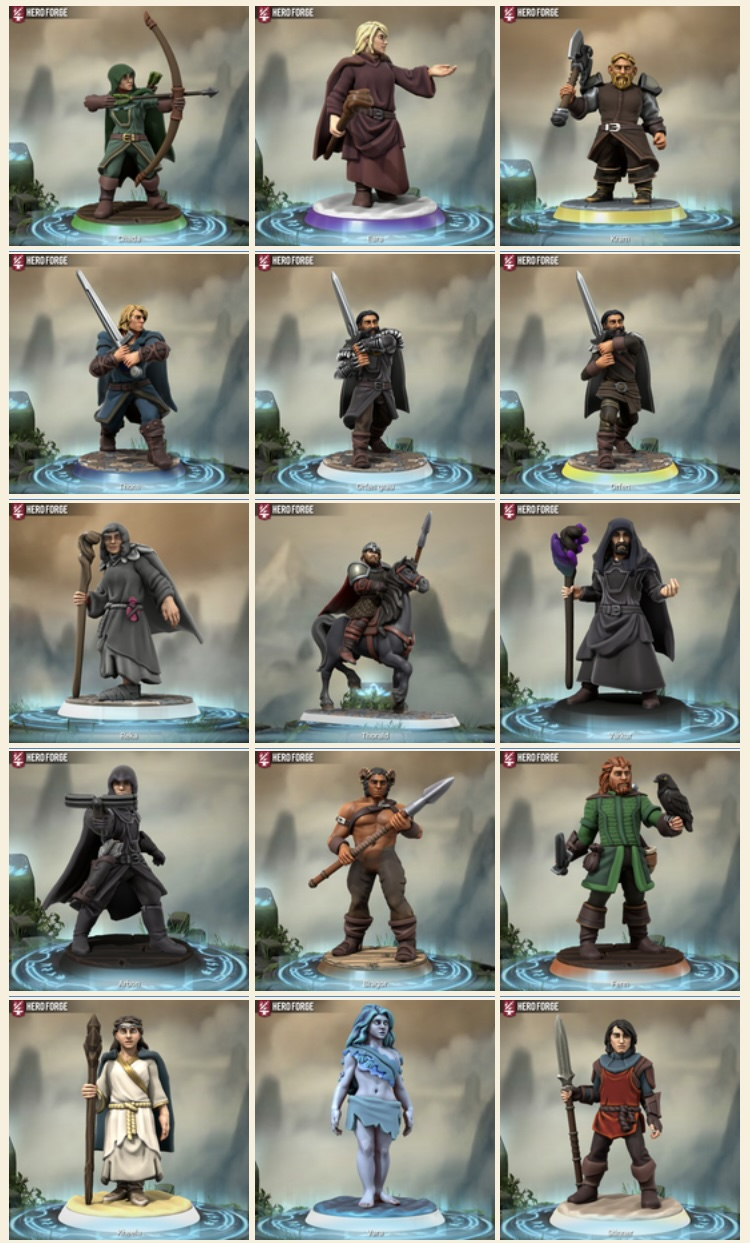
\includegraphics[width=0.3\linewidth]{Das Erbe des Wunderkindes/Bilder/3D mit der Heldenschmiede 1.jpg}
    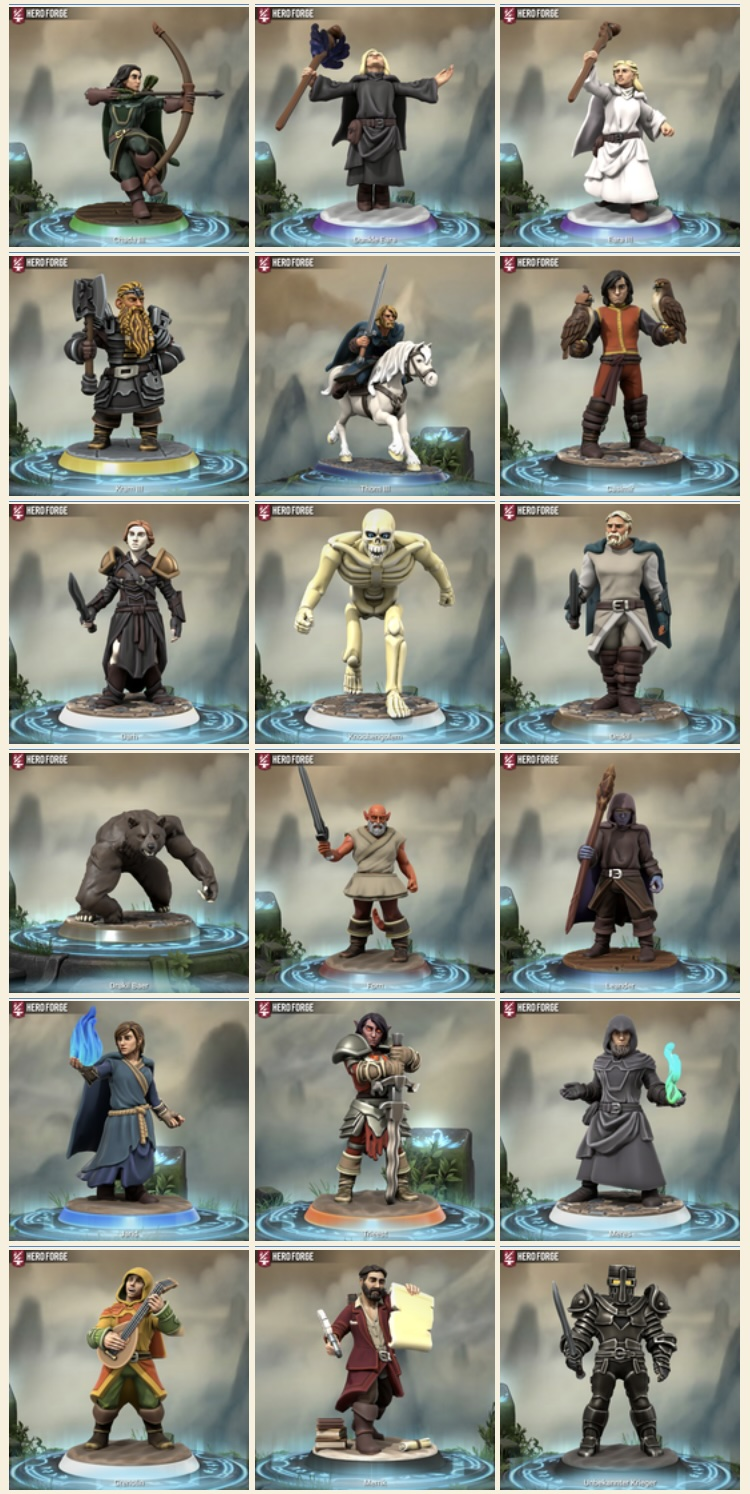
\includegraphics[width=0.3\linewidth]{Das Erbe des Wunderkindes/Bilder/3D mit der Heldenschmiede 2.jpg}\\
    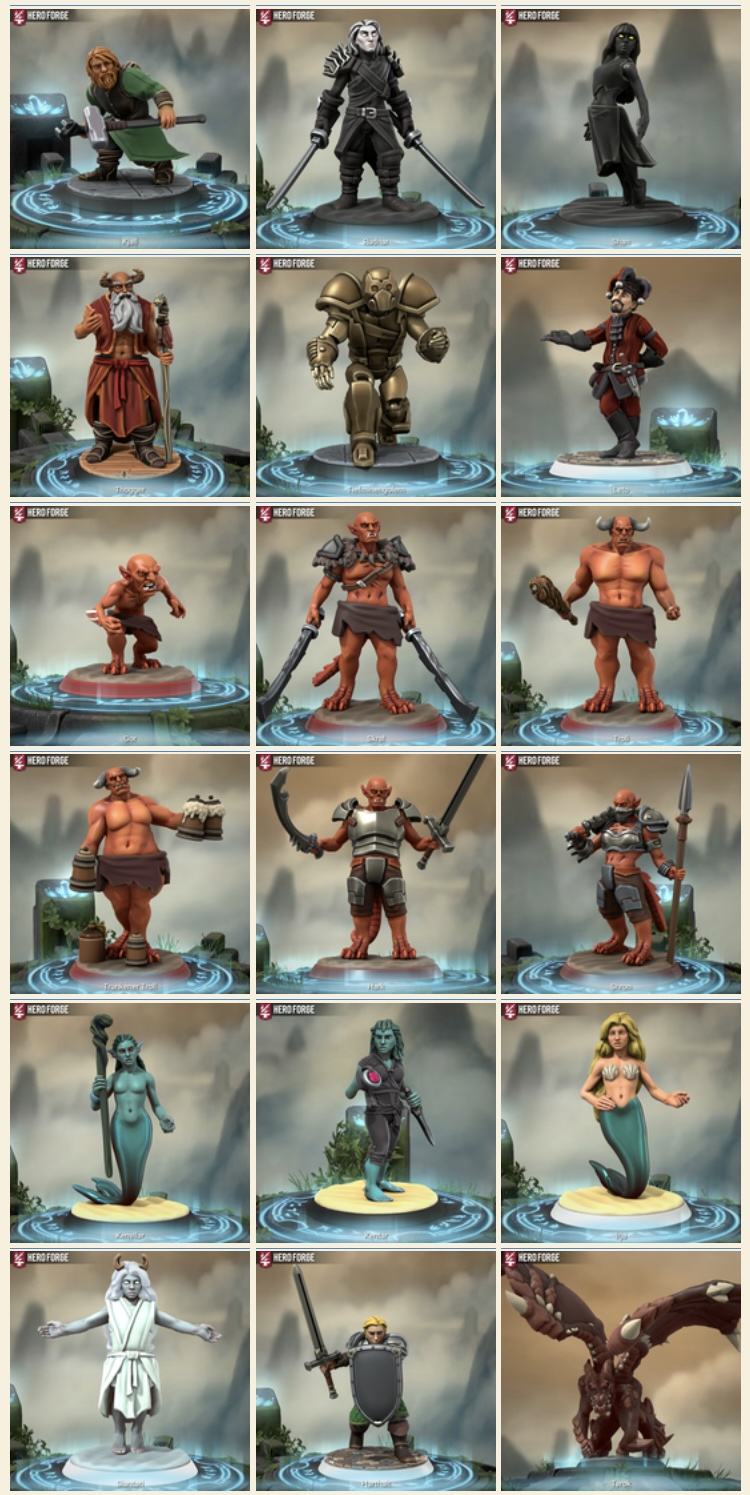
\includegraphics[width=0.3\linewidth]{Das Erbe des Wunderkindes/Bilder/3D mit der Heldenschmiede 3.jpg}
    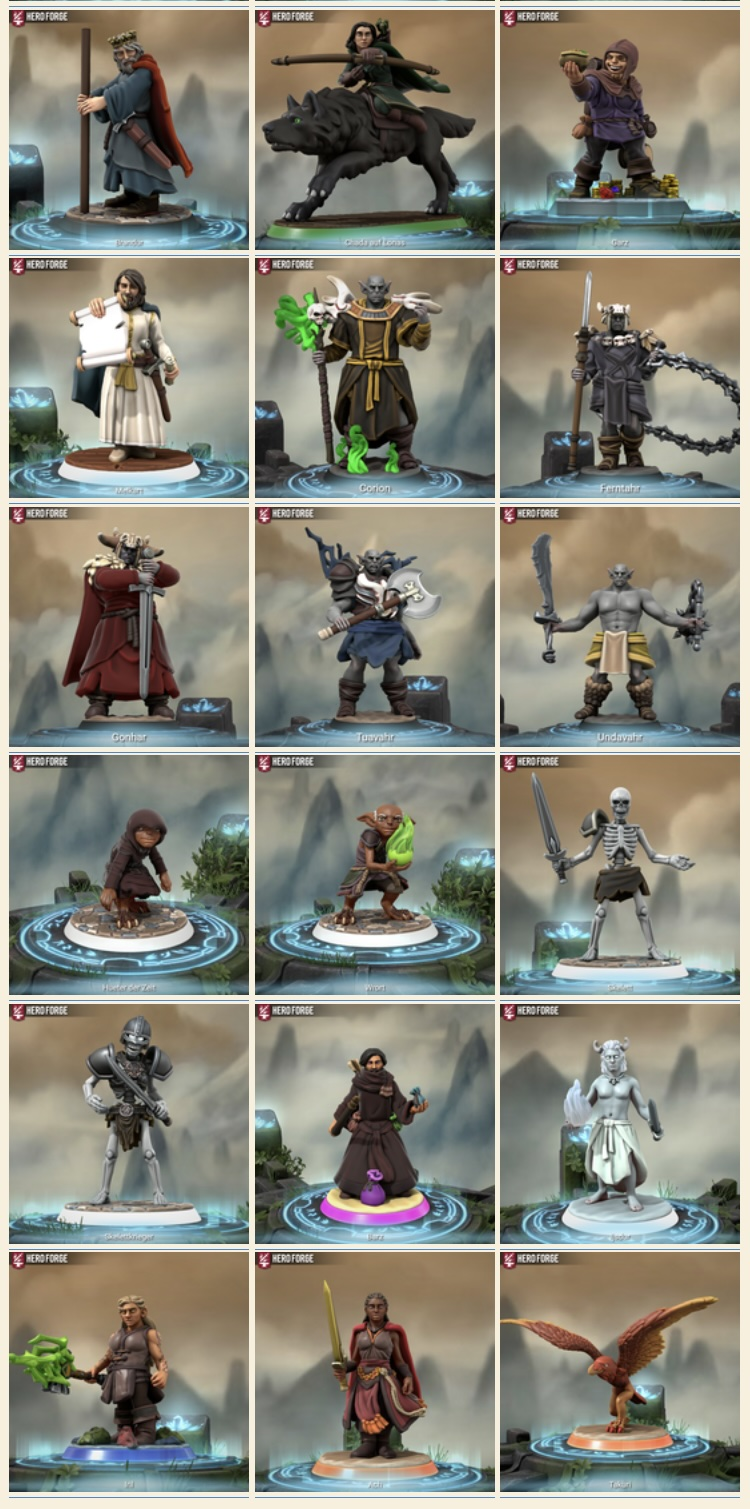
\includegraphics[width=0.3\linewidth]{Das Erbe des Wunderkindes/Bilder/3D mit der Heldenschmiede 4.jpg}
\end{figure}

Hallo liebe Andori,\bigskip

immer mal wieder kam das Thema "3D-Miniaturen für Andor" auf. Solche Figuren hätten sicherlich ihren Reiz, wobei ich die schönen gemalten Charaktere eigentlich doch lieber habe zum Spielen. Nichtsdestotrotz habe ich mal die Heldenschmiede (https://www.heroforge.com/) angeworfen und ein paar Beispielcharaktere erstellt. Vieles hat natürlich nicht perfekt funktioniert. Ich hab versucht, das beste rauszuholen :D

Drucken lassen werde ich mir keine, es hat mir einfach Spaß gemacht, sie zu designen und ich dachte, ich teile die Bilder mit euch :D

Ich finde die Seite auch ganz praktisch, um für etwaige Bilder auf Fan-Legenden Bild-Modelle von verschiedenen Charakteren zu erstellen, die man dann evtl. mit einem Bildbearbeitungsprogramm noch verfeinern kann.\bigskip

LG

Giftknödel


}



\newpage

\hintergrund{Andor Fan-Karte Inkarnate v2.0 textlos A4.jpg}

\thispagestyle{empty}%keine Header oder Footer auf dieser Seite

\textbf{ }

\end{document}